% Generated by Sphinx.
\def\sphinxdocclass{report}
\documentclass[letterpaper,10pt,english]{sphinxmanual}
\usepackage[utf8]{inputenc}
\DeclareUnicodeCharacter{00A0}{\nobreakspace}
\usepackage{cmap}
\usepackage[T1]{fontenc}
\usepackage{babel}
\usepackage{times}
\usepackage[Bjarne]{fncychap}
\usepackage{longtable}
\usepackage{sphinx}
\usepackage{multirow}


\title{The Stingray Schema-Based File Reader}
\date{May 11, 2015}
\release{4.4.6}
\author{S. Lott}
\newcommand{\sphinxlogo}{}
\renewcommand{\releasename}{Release}
\makeindex

\makeatletter
\def\PYG@reset{\let\PYG@it=\relax \let\PYG@bf=\relax%
    \let\PYG@ul=\relax \let\PYG@tc=\relax%
    \let\PYG@bc=\relax \let\PYG@ff=\relax}
\def\PYG@tok#1{\csname PYG@tok@#1\endcsname}
\def\PYG@toks#1+{\ifx\relax#1\empty\else%
    \PYG@tok{#1}\expandafter\PYG@toks\fi}
\def\PYG@do#1{\PYG@bc{\PYG@tc{\PYG@ul{%
    \PYG@it{\PYG@bf{\PYG@ff{#1}}}}}}}
\def\PYG#1#2{\PYG@reset\PYG@toks#1+\relax+\PYG@do{#2}}

\expandafter\def\csname PYG@tok@kr\endcsname{\let\PYG@bf=\textbf\def\PYG@tc##1{\textcolor[rgb]{0.00,0.44,0.13}{##1}}}
\expandafter\def\csname PYG@tok@kp\endcsname{\def\PYG@tc##1{\textcolor[rgb]{0.00,0.44,0.13}{##1}}}
\expandafter\def\csname PYG@tok@s1\endcsname{\def\PYG@tc##1{\textcolor[rgb]{0.25,0.44,0.63}{##1}}}
\expandafter\def\csname PYG@tok@kt\endcsname{\def\PYG@tc##1{\textcolor[rgb]{0.56,0.13,0.00}{##1}}}
\expandafter\def\csname PYG@tok@cs\endcsname{\def\PYG@tc##1{\textcolor[rgb]{0.25,0.50,0.56}{##1}}\def\PYG@bc##1{\setlength{\fboxsep}{0pt}\colorbox[rgb]{1.00,0.94,0.94}{\strut ##1}}}
\expandafter\def\csname PYG@tok@ow\endcsname{\let\PYG@bf=\textbf\def\PYG@tc##1{\textcolor[rgb]{0.00,0.44,0.13}{##1}}}
\expandafter\def\csname PYG@tok@s\endcsname{\def\PYG@tc##1{\textcolor[rgb]{0.25,0.44,0.63}{##1}}}
\expandafter\def\csname PYG@tok@w\endcsname{\def\PYG@tc##1{\textcolor[rgb]{0.73,0.73,0.73}{##1}}}
\expandafter\def\csname PYG@tok@kc\endcsname{\let\PYG@bf=\textbf\def\PYG@tc##1{\textcolor[rgb]{0.00,0.44,0.13}{##1}}}
\expandafter\def\csname PYG@tok@k\endcsname{\let\PYG@bf=\textbf\def\PYG@tc##1{\textcolor[rgb]{0.00,0.44,0.13}{##1}}}
\expandafter\def\csname PYG@tok@il\endcsname{\def\PYG@tc##1{\textcolor[rgb]{0.13,0.50,0.31}{##1}}}
\expandafter\def\csname PYG@tok@m\endcsname{\def\PYG@tc##1{\textcolor[rgb]{0.13,0.50,0.31}{##1}}}
\expandafter\def\csname PYG@tok@kd\endcsname{\let\PYG@bf=\textbf\def\PYG@tc##1{\textcolor[rgb]{0.00,0.44,0.13}{##1}}}
\expandafter\def\csname PYG@tok@o\endcsname{\def\PYG@tc##1{\textcolor[rgb]{0.40,0.40,0.40}{##1}}}
\expandafter\def\csname PYG@tok@c\endcsname{\let\PYG@it=\textit\def\PYG@tc##1{\textcolor[rgb]{0.25,0.50,0.56}{##1}}}
\expandafter\def\csname PYG@tok@kn\endcsname{\let\PYG@bf=\textbf\def\PYG@tc##1{\textcolor[rgb]{0.00,0.44,0.13}{##1}}}
\expandafter\def\csname PYG@tok@sx\endcsname{\def\PYG@tc##1{\textcolor[rgb]{0.78,0.36,0.04}{##1}}}
\expandafter\def\csname PYG@tok@sr\endcsname{\def\PYG@tc##1{\textcolor[rgb]{0.14,0.33,0.53}{##1}}}
\expandafter\def\csname PYG@tok@ss\endcsname{\def\PYG@tc##1{\textcolor[rgb]{0.32,0.47,0.09}{##1}}}
\expandafter\def\csname PYG@tok@sh\endcsname{\def\PYG@tc##1{\textcolor[rgb]{0.25,0.44,0.63}{##1}}}
\expandafter\def\csname PYG@tok@si\endcsname{\let\PYG@it=\textit\def\PYG@tc##1{\textcolor[rgb]{0.44,0.63,0.82}{##1}}}
\expandafter\def\csname PYG@tok@sb\endcsname{\def\PYG@tc##1{\textcolor[rgb]{0.25,0.44,0.63}{##1}}}
\expandafter\def\csname PYG@tok@sc\endcsname{\def\PYG@tc##1{\textcolor[rgb]{0.25,0.44,0.63}{##1}}}
\expandafter\def\csname PYG@tok@c1\endcsname{\let\PYG@it=\textit\def\PYG@tc##1{\textcolor[rgb]{0.25,0.50,0.56}{##1}}}
\expandafter\def\csname PYG@tok@sd\endcsname{\let\PYG@it=\textit\def\PYG@tc##1{\textcolor[rgb]{0.25,0.44,0.63}{##1}}}
\expandafter\def\csname PYG@tok@se\endcsname{\let\PYG@bf=\textbf\def\PYG@tc##1{\textcolor[rgb]{0.25,0.44,0.63}{##1}}}
\expandafter\def\csname PYG@tok@vg\endcsname{\def\PYG@tc##1{\textcolor[rgb]{0.73,0.38,0.84}{##1}}}
\expandafter\def\csname PYG@tok@vc\endcsname{\def\PYG@tc##1{\textcolor[rgb]{0.73,0.38,0.84}{##1}}}
\expandafter\def\csname PYG@tok@nt\endcsname{\let\PYG@bf=\textbf\def\PYG@tc##1{\textcolor[rgb]{0.02,0.16,0.45}{##1}}}
\expandafter\def\csname PYG@tok@nv\endcsname{\def\PYG@tc##1{\textcolor[rgb]{0.73,0.38,0.84}{##1}}}
\expandafter\def\csname PYG@tok@vi\endcsname{\def\PYG@tc##1{\textcolor[rgb]{0.73,0.38,0.84}{##1}}}
\expandafter\def\csname PYG@tok@mf\endcsname{\def\PYG@tc##1{\textcolor[rgb]{0.13,0.50,0.31}{##1}}}
\expandafter\def\csname PYG@tok@nl\endcsname{\let\PYG@bf=\textbf\def\PYG@tc##1{\textcolor[rgb]{0.00,0.13,0.44}{##1}}}
\expandafter\def\csname PYG@tok@no\endcsname{\def\PYG@tc##1{\textcolor[rgb]{0.38,0.68,0.84}{##1}}}
\expandafter\def\csname PYG@tok@nn\endcsname{\let\PYG@bf=\textbf\def\PYG@tc##1{\textcolor[rgb]{0.05,0.52,0.71}{##1}}}
\expandafter\def\csname PYG@tok@ni\endcsname{\let\PYG@bf=\textbf\def\PYG@tc##1{\textcolor[rgb]{0.84,0.33,0.22}{##1}}}
\expandafter\def\csname PYG@tok@bp\endcsname{\def\PYG@tc##1{\textcolor[rgb]{0.00,0.44,0.13}{##1}}}
\expandafter\def\csname PYG@tok@ne\endcsname{\def\PYG@tc##1{\textcolor[rgb]{0.00,0.44,0.13}{##1}}}
\expandafter\def\csname PYG@tok@nd\endcsname{\let\PYG@bf=\textbf\def\PYG@tc##1{\textcolor[rgb]{0.33,0.33,0.33}{##1}}}
\expandafter\def\csname PYG@tok@nf\endcsname{\def\PYG@tc##1{\textcolor[rgb]{0.02,0.16,0.49}{##1}}}
\expandafter\def\csname PYG@tok@na\endcsname{\def\PYG@tc##1{\textcolor[rgb]{0.25,0.44,0.63}{##1}}}
\expandafter\def\csname PYG@tok@nc\endcsname{\let\PYG@bf=\textbf\def\PYG@tc##1{\textcolor[rgb]{0.05,0.52,0.71}{##1}}}
\expandafter\def\csname PYG@tok@nb\endcsname{\def\PYG@tc##1{\textcolor[rgb]{0.00,0.44,0.13}{##1}}}
\expandafter\def\csname PYG@tok@gt\endcsname{\def\PYG@tc##1{\textcolor[rgb]{0.00,0.27,0.87}{##1}}}
\expandafter\def\csname PYG@tok@gu\endcsname{\let\PYG@bf=\textbf\def\PYG@tc##1{\textcolor[rgb]{0.50,0.00,0.50}{##1}}}
\expandafter\def\csname PYG@tok@gr\endcsname{\def\PYG@tc##1{\textcolor[rgb]{1.00,0.00,0.00}{##1}}}
\expandafter\def\csname PYG@tok@gs\endcsname{\let\PYG@bf=\textbf}
\expandafter\def\csname PYG@tok@gp\endcsname{\let\PYG@bf=\textbf\def\PYG@tc##1{\textcolor[rgb]{0.78,0.36,0.04}{##1}}}
\expandafter\def\csname PYG@tok@cm\endcsname{\let\PYG@it=\textit\def\PYG@tc##1{\textcolor[rgb]{0.25,0.50,0.56}{##1}}}
\expandafter\def\csname PYG@tok@s2\endcsname{\def\PYG@tc##1{\textcolor[rgb]{0.25,0.44,0.63}{##1}}}
\expandafter\def\csname PYG@tok@mo\endcsname{\def\PYG@tc##1{\textcolor[rgb]{0.13,0.50,0.31}{##1}}}
\expandafter\def\csname PYG@tok@mh\endcsname{\def\PYG@tc##1{\textcolor[rgb]{0.13,0.50,0.31}{##1}}}
\expandafter\def\csname PYG@tok@mi\endcsname{\def\PYG@tc##1{\textcolor[rgb]{0.13,0.50,0.31}{##1}}}
\expandafter\def\csname PYG@tok@gd\endcsname{\def\PYG@tc##1{\textcolor[rgb]{0.63,0.00,0.00}{##1}}}
\expandafter\def\csname PYG@tok@ge\endcsname{\let\PYG@it=\textit}
\expandafter\def\csname PYG@tok@go\endcsname{\def\PYG@tc##1{\textcolor[rgb]{0.20,0.20,0.20}{##1}}}
\expandafter\def\csname PYG@tok@cp\endcsname{\def\PYG@tc##1{\textcolor[rgb]{0.00,0.44,0.13}{##1}}}
\expandafter\def\csname PYG@tok@gi\endcsname{\def\PYG@tc##1{\textcolor[rgb]{0.00,0.63,0.00}{##1}}}
\expandafter\def\csname PYG@tok@gh\endcsname{\let\PYG@bf=\textbf\def\PYG@tc##1{\textcolor[rgb]{0.00,0.00,0.50}{##1}}}
\expandafter\def\csname PYG@tok@err\endcsname{\def\PYG@bc##1{\setlength{\fboxsep}{0pt}\fcolorbox[rgb]{1.00,0.00,0.00}{1,1,1}{\strut ##1}}}

\def\PYGZbs{\char`\\}
\def\PYGZus{\char`\_}
\def\PYGZob{\char`\{}
\def\PYGZcb{\char`\}}
\def\PYGZca{\char`\^}
\def\PYGZam{\char`\&}
\def\PYGZlt{\char`\<}
\def\PYGZgt{\char`\>}
\def\PYGZsh{\char`\#}
\def\PYGZpc{\char`\%}
\def\PYGZdl{\char`\$}
\def\PYGZhy{\char`\-}
\def\PYGZsq{\char`\'}
\def\PYGZdq{\char`\"}
\def\PYGZti{\char`\~}
% for compatibility with earlier versions
\def\PYGZat{@}
\def\PYGZlb{[}
\def\PYGZrb{]}
\makeatother

\begin{document}

\maketitle
\tableofcontents
\phantomsection\label{index::doc}


The Stingray Reader tackles four fundamental issues in
processing a file:
\begin{itemize}
\item {} 
How are the bytes organized?  What is the Physical Format?

\item {} 
Haw are the data objects organized?  What is the Logical Layout?

\item {} 
What do the bytes \emph{mean}?  What is the Conceptual Content?

\item {} 
How can we assure ourselves that our applications will work with this file?

\end{itemize}

The problem we have is that the schema is not always bound
to a given file nor is the schema clearly bound to an application program.
There are two examples of this separation between schema and content:
\begin{itemize}
\item {} 
We might have a spreadsheet where there aren't even column titles.

\item {} 
We might have a pure data file (for example from a legacy COBOL program)
which is described by a separate schema.

\end{itemize}

One goal of good software is to cope reasonably well with variability
of user-supplied inputs.  Providing data by spreadsheet is
often the most desirable choice for users.  In some cases, it's the
only acceptable choice.  Since spreadsheets are tweaked manually, they
may not have a simple, fixed schema or logical layout.

A workbook (the container of individual sheets)
can be encoded in any of a number of physical
formats: XLS, CSV, XLSX, ODS to name a few.  We would like our applications
to be independent of these physical formats.  We'd like to focus
on the logical layout.

Data supplied in the form of a workbook can suffer from numerous data quality issues.
We need to be assured that a file actually conforms to a required
schema.

A COBOL file parallels a workbook sheet in several ways. It also introduces
some unique complications. We'd like to provide a suite of tools that work
well with common spreadsheets as well as COBOL files, allowing some
uniformity in processing various kinds of data.


\chapter{Technology}
\label{index:technology}\label{index:the-stingray-schema-based-file-reader}
While this is 100\% Python, it's not \emph{simply} Python. The actual code
is built from this document.

\begin{notice}{warning}{Warning:}
The Code Did Not Come First

The document doesn't follow behind the code. The document \textbf{contains}
the code. The code is extracted from the document.
For details, see the {\hyperref[build:build]{\emph{Stingray Build}}} section.
\end{notice}


\chapter{Contents}
\label{index:contents}

\section{Introduction}
\label{introduction:intro}\label{introduction::doc}\label{introduction:introduction}
Given a workbook -- or any other ``flat'' file -- how is it organized?  What does it \emph{mean}?

How can we ignore details that are merely physical?
When is a change merely a logical layout variant with no semantic impact?
How do we isolate ourselves from these variations?

There are two user stories that we want to focus on.
\begin{itemize}
\item {} 
\textbf{Extract Transform and Load (ETL)}.   We've got a file of data
in the form of a workbook (``spreadsheet'') file or perhaps a flat (delimiter-free) COBOL file.
The \textbf{ET} portion of \textbf{ETL} may be part of a ``Big Data'' application:
it could be the mapper portion of a Hadoop Map-Reduce.

\item {} 
\textbf{Analysis}.  More specifically, Data Profiling.  We've got a file of data and we want to
examine it for frequencies, ranges and relationships.
A common use for this is to ``validate'' or ``unit test''
a file before attempting to process it.

\end{itemize}

In these cases, we don't want our applications to depend on
the physical file format.
We want to work equally well with CSV or XLSX versions of a file.

We'd like something like this to transparently handle workbook files in a variety of formats.
\begin{alltt}
def process\_sheet( sheet ):
    ``''``Separated to facilitate unit testing''``''
    counts= defaultdict( int )
    for rows in sheet.rows():
        \emph{process row}
    return counts

def main(args):
    for input in args.file:
        with workbook.open\_workbook( input ) as source:
            for name in source.sheets(): ❶
                sheet= source.sheet( name,
                    sheet.EmbeddedSchemaSheet, ❷
                    loader\_class=schema.loader.HeadingRowSchemaLoader ) ❸
                counts= process\_sheet( sheet )
                pprint( counts )
\end{alltt}

Note that this is wordy because it specifies a number of things explicitly.
\begin{itemize}
\item {} 
❶ \code{for name in source.sheets()} claims that \emph{all} sheets have valid data.
When this is not the case, more sophisticated name filtering
needs to be inserted into this loop.

\item {} 
❷ {\hyperref[sheet:sheet.EmbeddedSchemaSheet]{\code{sheet.EmbeddedSchemaSheet}}} states that the sheet has the schema
embedded in it.  For example, the headers in the first row of the sheet.
We can use {\hyperref[sheet:sheet.ExternalSchemaSheet]{\code{sheet.ExternalSchemaSheet}}} to specify
that an external schema must be loaded. For example, a separate sheet in this
workbook or perhaps a separate file.

\item {} 
❸ {\hyperref[schema_loader:schema.loader.HeadingRowSchemaLoader]{\code{schema.loader.HeadingRowSchemaLoader}}} states that the schema is
the first row of the sheet.  We can write other parsers for other sheets
with more complex or atypical layouts.

\end{itemize}

We've made these issues explicit because they are the source of complication
in otherwise simple applications. Parsing the header from \code{.csv} files is done
by a simple algorithm in the \code{csv} module. This algorithm isn't always
appropriate, and we need to be able to change it.


\subsection{Logical Layout Issues}
\label{introduction:logical-layout-issues}
Beyond physical format transparency, we want applications that are flexible with respect to the
the logical layout of coumns.  We'd like to be adaptable to changes to the names, number,
order and type of columns without a significant rewrite. We'd like
to isolate the column names or positions from the rest of our application processing.

We can do this by definining  small ``builder'' functions which isolate the
logical layout from the rest of the application.

We'd like something like this.

\begin{Verbatim}[commandchars=\\\{\}]
\PYG{k}{def} \PYG{n+nf}{build\PYGZus{}record\PYGZus{}dict}\PYG{p}{(} \PYG{n}{aRow} \PYG{p}{)}\PYG{p}{:}
    \PYG{k}{return} \PYG{n+nb}{dict}\PYG{p}{(}
        \PYG{n}{name} \PYG{o}{=} \PYG{n}{aRow}\PYG{p}{[}\PYG{l+s}{\PYGZsq{}}\PYG{l+s}{some column}\PYG{l+s}{\PYGZsq{}}\PYG{p}{]}\PYG{o}{.}\PYG{n}{to\PYGZus{}str}\PYG{p}{(}\PYG{p}{)}\PYG{p}{,}
        \PYG{n}{address} \PYG{o}{=} \PYG{n}{aRow}\PYG{p}{[}\PYG{l+s}{\PYGZsq{}}\PYG{l+s}{another column}\PYG{l+s}{\PYGZsq{}}\PYG{p}{]}\PYG{o}{.}\PYG{n}{to\PYGZus{}str}\PYG{p}{(}\PYG{p}{)}\PYG{p}{,}
        \PYG{n+nb}{zip} \PYG{o}{=} \PYG{n}{aRow}\PYG{p}{[}\PYG{l+s}{\PYGZsq{}}\PYG{l+s}{zip}\PYG{l+s}{\PYGZsq{}}\PYG{p}{]}\PYG{o}{.}\PYG{n}{to\PYGZus{}digit\PYGZus{}str}\PYG{p}{(}\PYG{l+m+mi}{5}\PYG{p}{)}\PYG{p}{,}
        \PYG{n}{phone} \PYG{o}{=} \PYG{n}{aRow}\PYG{p}{[}\PYG{l+s}{\PYGZsq{}}\PYG{l+s}{phone}\PYG{l+s}{\PYGZsq{}}\PYG{p}{]}\PYG{o}{.}\PYG{n}{to\PYGZus{}digit\PYGZus{}str}\PYG{p}{(}\PYG{p}{)}\PYG{p}{,}
    \PYG{p}{)}
\end{Verbatim}

The column names and data conversions are isolated to this
function only.  As the source schemata evolve, we can update an
application to add variations on this function.

From this, we can build Python objects using the following:
\begin{alltt}
def build\_object( record\_dict ):
    return ObjectClass( **row\_dict )
\end{alltt}

We can combine the two steps like this:

\begin{Verbatim}[commandchars=\\\{\}]
\PYG{k}{def} \PYG{n+nf}{object\PYGZus{}iter}\PYG{p}{(} \PYG{n}{source} \PYG{p}{)}\PYG{p}{:}
    \PYG{k}{for} \PYG{n}{row} \PYG{o+ow}{in} \PYG{n}{source}\PYG{p}{:}
        \PYG{n}{rd}\PYG{o}{=} \PYG{n+nb+bp}{self}\PYG{o}{.}\PYG{n}{build\PYGZus{}record\PYGZus{}dict}\PYG{p}{(} \PYG{n}{row} \PYG{p}{)}
        \PYG{k}{yield} \PYG{n+nb+bp}{self}\PYG{o}{.}\PYG{n}{build\PYGZus{}object}\PYG{p}{(} \PYG{n}{rd} \PYG{p}{)}
\end{Verbatim}

This design breaks processing into two parts because the logical layout mapping
from workbook rows to Python objects is never trivial.  This is subject to change
with minimal notice.
Experience indicates that it's better to break the processing into two discrete
steps so that transformations are easier to manage and extend.

We can then use this iterator to process rows of a sheet.
\begin{alltt}
def process\_sheet( sheet ):
    counts= defaultdict( int )
    for app\_object in object\_iter( sheet.rows() ):
        \emph{process the app\_object}
    return counts
\end{alltt}

We'll show concrete implementation examples in the {\hyperref[demo/index:demo]{\emph{Stingray Demo Applications}}} section.


\subsection{Deeper Issues}
\label{introduction:deeper-issues}
Processing a workbook (or other flat file) means solving two closely-related schema problems.
\begin{itemize}
\item {} 
Decoding the ``Physical Format''.  Format is the organization of bytes from
which we can decode Python objects (e.g., decode a string to lines
of text to atomic fields).  A workbook should make the physical format irrelevant.

\item {} 
Mapping to the ``Logical Layout''. That is, the semantic mapping from Python
items (e.g., strings) to meaningful data elements in our problem domain (e.g., customer zip codes.)

\end{itemize}

Both of these are implementation details for some \emph{Conceptual Content}.  The
conceptual schema is the \emph{meaning} behind the encoded data.

Often, the physical format issue is addressed by using a well-known (or even standardized) file format:
CSV, XLSX, XML, JSON, YAML, etc.
We'll start with just the workbook formats CSV, XLSX and ODS.

We'll ignore JSON and YAML for the time being. We should be able to extend our
model from highly structured data to semi-structured data, including JSON, YAML,
and even documents created with outliner tools.

We'll expand on our model to include COBOL files. In many cases, they will parallel
workbooks. In some cases, however, they introduce some complexity.

The logical layout issue is not as easy to address as the physical format issue.
A file is either compliant with a physical format or it's not.  Why is logical
layout more complex than physical format? We've seen at least four common reasons:
\begin{itemize}
\item {} 
\textbf{Bullfeathers}.  Also known as Semantic Heterogeneity.
You call them ``customers'' because they have
a contract and pay money for services.  Marketing, however, calls their
prospects ``customers'' even though there is no contract in place.
Same word.  Different semantics.

Yes, this a ``problem domain'' issue.  No, there's no technical solution short
of a complete ontology for each data item.

We'll need a design with enough flexibility to handle
the semantic matching expediently.

\item {} 
\textbf{Buffoonery}.  Is ``CSTID'' the ``customer id number''?
Or is it the ``Commercial Status ID''?  Or is it the ``Credit Score
Time Interval Delta''?  Or is it something entirely unrelated that merely
happens to be shoved into that field?

Yes, this is ``code rot.'' Even with careful format definitions, this kind of thing happens as software
matures. No, there's no technical solution short of firing all the managers
who make short-sighted decisions.

We'll need a design that has the flexibility to cope with variant abbreviations for column names.

\item {} 
\textbf{Bad Management}.  At some point in the past, the ``Employees Here'' and ``Total Employees''
were misused by an application.  The problem was found--and fixed--but
there is some ``legacy'' data that has incorrect values.  What now?

Yes, this is a data stewardship problem.

This leads to rather complex designs where the mapping from source to target
is dependent on some external context for the source data.

\item {} 
\textbf{Bugs}.  The field named ``Effective Date'' is really the \emph{Reported Date}.
The field name ``Supplied Date'' is really the \emph{Effective Date}.
The field labeled ``Reported Date'' isn't populated consistently and doesn't
seem to have any meaning.  Really.

There's a fine line between ``technical debt'' and ``code rot.'' Our point
is not to sort out the root cause of the problem.

We need flexibility to handle bugs as well as other problems.

\end{itemize}

There is always an underlying \emph{Conceptual Schema}.  It often has numerous
variant implementations, each with a unique collection of errors and anomalies.


\subsection{Misdirections}
\label{introduction:misdirections}
Our canonical examples are the \code{csv} and the \code{xlrd} package.
These offer handy ways to read workbooks. However, they're far from ideal.
Both of these show eager processing and flat structures.

We have an additional consideration when it comes to data conversions.
We have to avoid the attractive nuisance of a Domain Specific Language (DSL)
for mappings and conversions.

We have to be cautious of trying too hard to leverage the \code{csv} module's
row-as-dictionary view of data.
The \code{csv.DictReader} approach -- implicitly creating a dict instead of a sequence --
fails us when we have to work with COBOL or Fixed Format files.
These non-spreadsheet files may not be close to First Normal Form.
COBOL files have repeating groups which
require numeric indexes in addition to column names.

For semi-structured data (JSON, YAML our an outline) there are fewer
constraints on the data, leading to a more complex normalization step and possible
row validation rules. We'd like to retain a relatively simple schema
in spite of the potential complexity of these files.

The \code{csv} approach of \textbf{eagerly} building a row doesn't work
for COBOL files because of the \code{REDEFINES} clause.  We can't reliably
build the various ``cells'' available in a COBOL schema, since some of
those values may turn out to be invalid. COBOL requires lazily building a row
based on which REDEFINES alias is relevant.

We also have to avoid the attractive nuisance of trying to create a
``data mapping DSL''.  This is seductive because a data mapping
is a triple of target, source and conversion. It seems like we could write some language
that encodes these three things in a handy summary like this:

\begin{Verbatim}[commandchars=\\\{\}]
\PYG{n}{target} \PYG{o}{=} \PYG{n}{source}\PYG{o}{.}\PYG{n}{conversion}\PYG{p}{(}\PYG{p}{)}
\end{Verbatim}

Since this is -- effectively -- Python code, there's no real reason
for creating a DSL when we can just use Python.


\subsubsection{Historical Solutions}
\label{introduction:historical-solutions}\begin{quote}

``Those who cannot remember the past are condemned to repeat it.''
--George Santayana
\end{quote}

We'll look at four solutions in their approximate historical order.

The {\hyperref[introduction:cobol-schema-solution]{COBOL Schema Solution}}  is still relevant
to modern Python programmers.

The {\hyperref[introduction:dbms-schema-solution]{DBMS Schema Solution}} is available, but isn't compeletly universal.
It doesn't apply well to files outside the database.

The {\hyperref[introduction:csv-schema-solution]{CSV Schema Solution}} often introduces more problems than it solves.

There is an {\hyperref[introduction:xml-non-solution]{XML Non-Solution}}.  While XML is relevant, it is not the \emph{trivial} solution
that some folks seem to hope for.  At best, it offers us XSD, which may be too sophisticated
for the problem we're trying to solve.

For semi-structured data (JSON, YAML and outlines), we need more than a simple
schema definition. We need processing rules to reformat and validate the inputs
as well.


\subsection{COBOL Schema Solution}
\label{introduction:cobol-schema-solution}
A significant feature of the COBOL language is the Data Definition Entry (DDE)
used in the data and environment divisions of the source.  This was a hierarchical
structure that defined the various items in a single record of a file.

Hierarchical.  Like XML.

COBOL best practice was essentially DRY:
developers would keep the definitions as separate modules
under ordinary source code control.
Every application that worked with a given file would import the DDE for
that file.

Clearly, the binding between schema and file is a two-step operation.
There's a compile-time binding between schema and application.  There's a
run-time binding between application and file.

Just as clearly, this is subject to all kinds of mysterious problems when
schema definition modules are cloned and then modified, leaving it unclear
which version is correct.  Also, when a schema definition was modified and not
all programs were properly recompiled, some programs worked with some
files, other programs didn't.

Since the schema wasn't formally bound to the file, it was particularly easy
to have files without any known schema.  Ideally, the file name included
some schema hint.

What's relevant for Python programmers is the central idea of a schema
being external to any specific application.

To this, we would like to assure that the schema was bound to the relevant
files.  This is much more difficult to achieve in practice, but there are some
approaches that can work through manually managing file names.


\subsection{DBMS Schema Solution}
\label{introduction:dbms-schema-solution}
A Database Management System (DBMS) -- whether relational or hierarchical
or columnar or networked or whatever -- addresses the problems with
flat files and the separation between application program, physical format,
logical layout, and operating system file.
A DBMS provides a complete logical/physical schema separation

The physical files are managed by the DBMS.  Our applications are now
independent of all physical file structure. They're often independent of
OS considerations, too.

The logical ``table structure'' (or ``document'' or whatever is offered) is distinct
from the files.  The logical schema it tightly bound to
the data itself.  When using SQL, for example, the column names and data types
are available as part of the execution of each SQL query.

This binding between data is schema is ideal.

Sadly, it doesn't apply to separate files.  Only to databases as a whole.

If file transfers are replaced with SQL queries (or web services requests)
then schema is discoverable from the database (or web service).  However, the
problem we're addressing here is file transfer.  So this
solution is inappropriate except as a guidepost.


\subsection{CSV Schema Solution}
\label{introduction:csv-schema-solution}
A workbook (or ``spreadsheet'') may or may not have schema
information. There may be a header row, a separate sheet, a separate
document, or nothing.

The workbook may have any of a large
number of physical formats: \code{.XLS} (i.e., native) \code{.XLSX} or \code{.CSV}.
The format is irrelevant to the presence or absence of a schema.

One common way to embed schema information
is to assure that the first row of each sheet within a workbook has
the schema information.  This is the ``column titles'' solution.
\begin{itemize}
\item {} 
This isn't done consistently.  Column titles are omitted.
Sometimes the titles occupy multiple rows.
Sometimes the sheet itself has a heading/body format where there's
irrelevant rows which must be filtered out.

\item {} 
This is subject to all kinds of buffoonery.  Column titles can
be tweaked manually.

\item {} 
The data type information is bound to each cell; the column title
provides no usable type information.

Exacerbating this is the way that anything number-like becomes a floating-point
number.  Zip codes, punctuation-free phone numbers and social security numbers,
etc., all become floating-point numbers.  This means they lose their
leading zeroes, making zip-code matching particularly painful.

\end{itemize}

Another common case is--of course--to omit schema information entirely.
This devolves to the {\hyperref[introduction:cobol-schema-solution]{COBOL Schema Solution}} where the schema
information must be incorporated as a separate, reusable module of some kind.

A less common case is to include a separate sheet in the workbook (or worse, a separate file)
with schema information.  A separate sheet in a workbook is at least bound
with the data.  A separate schema description file (even if bound in a ZIP archive) can get
unbound from the data.

While there are numerous problems, workbooks are a very common way to exchange
data.  It's not sensible to pretend they don't exist.

\begin{notice}{warning}{Warning:}
It Won't Go Away

We can't
paraphrase Jamie Zawinski and say

``Some people, when confronted with a problem, think `I know,
I'll use {[}a spreadsheet{]}.'  Now they have two problems.''

We do need to process this data irrespective of the issues.
\end{notice}

We need a suitable, Pythonic solution to the schema problem when confronted
with data in a spreadsheet.


\subsection{XML Non-Solution}
\label{introduction:xml-non-solution}
Weirdly, XML fans will claim we should use XML, stating the XML is ``self-defining''.
Their claim is that somehow this \emph{solves} the schema problem.  This statement can be
misleading.

For our purposes, XML is a kind of physical format.  An XML document without
a referenced (or embedded) XSD lacks any semantic information.
Even then, an XSD can be helpful, but not
sufficient.  The type definitions in an XSD could be unclear, ambiguous or
simply wrong.

An XSD document can be a good, useful schema definition.  It can also be riddled
with buffoonery, bad management and bugs.  It isn't magically \emph{perfect}.  It
merely frees us from physical format considerations.

We can -- to an extent -- leverage elements of PyXSD (\href{http://pyxsd.org}{http://pyxsd.org})
to create Python classes from an XSD schema.  This package could
help by providing a standard class structure for a schema
defined in Python.  In particular, the \code{pyxsd.schema} module contains
some of what we're going to use.

XSD is a bit too complex for this problem domain.  Spreadsheets don't make use of the
sophisticated modeling available in XSD.  A spreadsheet is a flat list of
of a few simple types (float, string, date-encoded-as-float.)   A
COBOL DDE is a hierarchy of of a few simple types (display, comp-3).
All we can really do is borrow some concepts and terminology.


\subsection{Summary}
\label{introduction:summary}
Physical format independence is available with some file formats.
Sadly, others -- which are still in active use -- require a great deal
of schema information merely to decode the physical format.

Logical layout is generally a feature of the application program
as well as the data.  In a SQL-based data access, the column
names in a \code{SELECT} statement amount to a binding between application and schema.

While we can make some kinds of simple
applications which are completely driven by metadata, we can't easily
escape the need to customize and deal with variations.
Therefore, we need to have application programs which can
tolerate physical format changes without complaint.

We would like an application program that can work with
``minor'' variations on a logical layout.  That is, the order
of columns, or minor spelling changes to a column name can be
handled gracefully.

We'd like our batch processing applications to have a command-line
interface something like this.

\begin{Verbatim}[commandchars=\\\{\}]
python \PYGZhy{}m some\PYGZus{}app \PYGZhy{}l layout\PYGZus{}2 some\PYGZus{}file.xyz
\end{Verbatim}

The \code{-l layout\_2} provides logical layout information. This defines the ``application-level'' schema information.

The \code{some\_file.xyz} could be \code{some\_file.xls} or \code{some\_file.ods},
allowing transparent changes to physical format.


\section{Design Considerations}
\label{design:design-considerations}\label{design::doc}
There are several important data representation issues. We'll look at
{\hyperref[design:workbook-schema-issues]{Workbook Schema Issues}} and {\hyperref[design:some-cobol-file-issues]{Some COBOL File Issues}} that
will inform the rest of the design.


\subsection{Workbook Schema Issues}
\label{design:workbook-schema-issues}
There are several sensible ways to represent workbook schema information.
Two of these are seen in the wild, and must be handled gracefully. Others
could be seen, and should be part of the use cases for this package.
\begin{enumerate}
\item {} 
One (or more) rows in each workbook sheet that provides the attribute
name.  The type is often left implicit.  This is often bound to the
data, making it quite useful in practice.

\item {} 
A distinct workbook sheet that lists name (and optionally type)
for each attribute.  Offset and size can
also be provided, making this useful for fixed-format COBOL files.
This may be bound to data in a separate sheet of the same workbook,
making it more likely to be useful. If it describes a COBOL file,
however, the binding is more tenuous.

\item {} 
A Python module that's built from source information.  This
allows us to trivially \code{import schema.foo} and have lots of cool
classes and functions in the \code{schema.foo} module. Ideally the
module is properly bound to the file, but there's little guarantee
of this.

\item {} 
Some standardized metadata format.  XSD (or even XMI) pops into mind.
These are detailed and potentially useful.
This is vanishingly rare in practice. The external XSD may not
be bound in any way to the data.

\end{enumerate}

Options 1 and 2 (workbook-based schema) cover over 99\%
of the cases in practice.  While the data is casual and error-prone, it's
often readily available.

Option 3 (a Python module) -- while cool -- breaks the DRY
principle.  Refreshing a Python schema when a source \code{.XLS} document
changes means that we have a multi-step binding: document to schema followed
by schema to application.

Option 4 is rarely used in practice.  In the rare cases when an organization
will consent to providing XSD files, they're often prepared separately
from the data and do not actually reflect the application software
that is used to build the data file.

How do we extend this to handle COBOL DDE's?

How do we extend this to handle JSON, YAML, or XML?

Clearly, we need to load schema information from a source every time
it's needed.  There are two paths:
\begin{itemize}
\item {} 
Either we'll parse the embedded schema buried in each
sheet of a workbook,

\item {} 
or we'll load an external schema definition from
a file.

\end{itemize}

We'll need to design schema loaders as well as data extractors which
depend on the schema loaders.


\subsection{Some COBOL File Issues}
\label{design:some-cobol-file-issues}
When dealing with ``Flat Files'' from legacy COBOL problems, there are several
additional problems that need to be solved.
\begin{enumerate}
\item {} 
The files have a fixed field layout, without delimiters.
This means that the offset of each field must be used to
decompose the record into its individual elements.

\item {} 
Numeric fields can have an implied decimal point, making
it difficult to determine the value of a string of digits.
The COBOL DDE is essential for parsing the file contents.

\item {} 
COBOL can make use of numeric data represented in a variety
of ``Computational'' forms.  The ``Computational-3'' (``COMP-3'')
form is very popular and rather complex because decimal digits are
packed two per byte and the final half-byte encodes
sign information.

\item {} 
The string data may be encoded in EBCDIC bytes.

\item {} 
COBOL encourages the use of data aliases (or ``unions'') via the \code{REDEFINES} clause.
Without the entire unviverse of COBOL programs that work with a given file,
the general handling of \code{REDEFINES}
data elements can become an insoluable problem.
Only lazy field access can work;
eager creation of individual cell values is doomed because a
\code{REDEFINES} alternative may be defined over invalid data.

\item {} 
COBOL has an \code{OCCURS DEPENDING ON} (ODO) feature where one attribute
determines the size of another attribute. This means the data
of every attribute after the ODO attribute has a location which varies.
The positions within the flat file cannot be computed statically.

\end{enumerate}

Generally, COBOL files are defined by a ``Data Definition Entry'' (DDE)
that provides the record layout.
It's essential to
parse this source DDE, which has the original COBOL
definition for the file.  A schema can be built from the parsed DDE.
There's no good reason to rely on any intermediate description separate from
the DDE's themselves.


\section{The \texttt{stingray} Package}
\label{package::doc}\label{package:the-stingray-package}
The \code{stingray} package implements a Schema-based File Reader.
This allows us to use flat-file and workbook data from Python without having
to clone an application for each physical file format or logical layout.

It also allows us to use semi-structured data like JSON, YAML or an outline.
This can be handled consistently with structured data.

This package includes
\begin{itemize}
\item {} 
A definition for ``workbook'', ``sheet'' and ``cell''.  This can subsume \code{csv},
\code{xlrd} as well as XML parsers for XLSX and ODS files.  This makes the
physical format transparent to an application.

\item {} 
A definition for a schema.  Not a complex XSD, but the limited,
flat schema appropriate for rows in sheets of a workbook in approximately First Normal Form.
This is extended to handle the simple hierarcical COBOL features.

\item {} 
Classes to load a schema that's embedded either in a sheet or in a separate file.

\item {} 
A COBOL schema loader as an extension to the default loaders.

\end{itemize}

This depends on Python 3.3.

The structure of the \code{stingray} package is as follows.
\begin{itemize}
\item {} 
\code{\_\_init\_\_.py}.  Some essential overhead.  See {\hyperref[stingray_init:stingray-init]{\emph{stingray \_\_init\_\_.py}}}.

\item {} 
\code{cell.py}.  {\hyperref[cell:cells]{\emph{Cell Module -- Data Element Containers and Conversions}}} defines the \code{Cell}
class hierarchy.  Imported as \code{stingray.cell}.

\item {} 
\code{sheet.py}.  {\hyperref[sheet:sheets]{\emph{Sheet Module -- Sheet and Row Access}}} defines the \code{Sheet} class hierarchy
that supports sheets with embedded as well as external schema.
Imported as \code{stingray.sheet}.

\item {} 
\code{workbook.py}.  The {\hyperref[workbook/index:workbook]{\emph{Workbook Package -- Uniform Wrappers for Workbooks}}} families.
Imported as \code{stingray.workbook}.

\item {} 
\code{schema}.  This package defines a schema and schema loaders.
\begin{itemize}
\item {} 
\code{\_\_init\_\_.py}.  {\hyperref[schema:schema]{\emph{Schema Package -- Schema and Attribute Definitions}}}.  Imported as \code{stingray.schema}.
This is the generic, flat schema and superclasses for the
more complex COBOL schema.

\item {} 
\code{loader.py}.   {\hyperref[schema_loader:schema-loader]{\emph{Schema Loader Module -- Load Embedded or External Schema}}}.
A loader for the generic, flat schema.  Imported as \code{stingray.schema.loader}.
Applications will often extend schema loaders to handle peculiar formats
or multi-line headings or other workbook formatting.

\end{itemize}

\item {} 
\code{cobol}.  This package extends a schema and schema loaders to handle COBOL files.
\begin{itemize}
\item {} 
\code{\_\_init\_\_.py}.  {\hyperref[cobol:cobol]{\emph{The COBOL Package}}}.
Imported as \code{stingray.cobol}.
These are extensions to \code{stingray.cell}, \code{stingray.sheet} and \code{stingray.workbook}.

\item {} 
\code{loader.py} {\hyperref[cobol_loader:cobol-loader]{\emph{COBOL Loader Module -- Parse COBOL Source to Load a Schema}}}.
A loader for COBOL-syntax schema.
Imported as \code{stingray.cobol.loader}.

\item {} 
\code{defs.py}. {\hyperref[cobol_defs:cobol-defs]{\emph{COBOL Definitions Module -- Handle COBOL DDE's}}}.
Base definitions used by both \code{\_\_init\_\_.py} and \code{loader.py}.

\end{itemize}

\item {} 
\code{snappy}. This module is a minimal implementation of a reader for files written
with Snappy compression.

\item {} 
\code{protobuf}. This module is a minimal implementation of a reader for objects represented
using protobuf.

\end{itemize}


\subsection{stingray \texttt{\_\_init\_\_.py}}
\label{stingray_init:stingray-init}\label{stingray_init::doc}\label{stingray_init:stingray-init-py}
This is approximately pure overhead required to make a Python package.
\phantomsection\label{stingray_init:module-__init__}\index{\_\_init\_\_ (module)}
\begin{Verbatim}[commandchars=\\\{\}]
\PYG{l+s+sd}{\PYGZdq{}\PYGZdq{}\PYGZdq{}stingray \PYGZhy{}\PYGZhy{}  Schema\PYGZhy{}based File Reader helps handle physical format and logical}
\PYG{l+s+sd}{layout of workbooks and flat files.}

\PYG{l+s+sd}{Requires Python 3.3, xlrd 0.9.2}
\PYG{l+s+sd}{\PYGZdq{}\PYGZdq{}\PYGZdq{}}
\PYG{n}{\PYGZus{}\PYGZus{}version\PYGZus{}\PYGZus{}} \PYG{o}{=} \PYG{l+s}{\PYGZdq{}}\PYG{l+s}{4.4.6}\PYG{l+s}{\PYGZdq{}}
\end{Verbatim}


\section{Cell Module -- Data Element Containers and Conversions}
\label{cell:module-cell}\label{cell:cell-module-data-element-containers-and-conversions}\label{cell::doc}\label{cell:cells}\index{cell (module)}
The point of a {\hyperref[cell:cell.Cell]{\code{cell.Cell}}} is two-fold:
\begin{itemize}
\item {} 
\textbf{Capture}.  That is, decode the information in the source file into
a Python object that represents the source spreadsheet value.
For XLS or XLSX formats, there are a variety of cell data types.
For CSV, all cells are text.
For a fixed format file, we may have to exploit the physical format information
to properly decode the bytes or characters.  We may even have to
cope with EBCDIC or packed decimal conversions.

\item {} 
\textbf{Convert}. Provide the cell value coerced to another Python type.
This is rather open-ended; it's hard to provide a comprehensive list of
types to which data can be converted.

\end{itemize}


\subsection{Capture Use Case}
\label{cell:capture-use-case}
The \textbf{Capture} use case is defined by our physical formats. We have several places
to look for source data formats:
\begin{itemize}
\item {} 
\code{xlrd}.

\item {} 
XSLX (ECMA 376).

\item {} 
Apple Numbers.

\end{itemize}

\code{xlrd} identifies the follow cell types found in XLS workbooks.

\begin{tabulary}{\linewidth}{|L|L|L|}
\hline
\textsf{\relax 
Type symbol
} & \textsf{\relax 
Type number
} & \textsf{\relax 
Python value
}\\
\hline
XL\_CELL\_EMPTY
 & 
0
 & 
empty string `'
\\

XL\_CELL\_TEXT
 & 
1
 & 
a Unicode string
\\

XL\_CELL\_NUMBER
 & 
2
 & 
float
\\

XL\_CELL\_DATE
 & 
3
 & 
float
\\

XL\_CELL\_BOOLEAN
 & 
4
 & 
int; 1 means TRUE, 0 means FALSE
\\

XL\_CELL\_ERROR
 & 
5
 & 
int representing internal Excel codes; for a text representation, refer to the supplied dictionary error\_text\_from\_code
\\

XL\_CELL\_BLANK
 & 
6
 & 
empty string `'. Note: this type will appear only when open\_workbook(..., formatting\_info=True) is used.
\\
\hline\end{tabulary}


An XLSX (per ECMA 376, section 18.18.11) or ODS provides a similar list of cell types.  The data is always encoded as a proper string that can be converted (if necessary) based on the type code.

\begin{tabulary}{\linewidth}{|L|L|}
\hline
\textsf{\relax 
Enumeration Value
} & \textsf{\relax 
Description
}\\
\hline
\code{b} (Boolean)
 & 
Cell containing a boolean.
\\

\code{d} (Date)
 & 
Cell contains a date in the ISO 8601 format.
\\

\code{e} (Error)
 & 
Cell containing an error.
\\

\code{inlineStr} (Inline String)
 & 
Cell containing an (inline) rich string, i.e., one not in the shared string table. If this cell type is used, then the cell value is in the is element rather than the v element in the cell (c element).
\\

\code{n} (Number)
 & 
Cell containing a number.
\\

\code{s} (Shared String)
 & 
Cell containing a shared string.
\\

\code{str} (String)
 & 
Cell containing a formula string.
\\
\hline\end{tabulary}


Dates formatted as strings are -- always -- a problem. There's no generic solution.  An application may need to write suitable extensions to handle this.
See below under {\hyperref[cell:conversion-functions]{Conversion Functions}}.

We should depend on the \code{locale} module to provide proper format strings for converting between date and string.

An Apple Numbers spreadsheet appears to have the following cell types. Some of the
tags appear to have no value, so their purpose is unclear.

\begin{tabulary}{\linewidth}{|L|L|}
\hline
\textsf{\relax 
Tag
} & \textsf{\relax 
Description
}\\
\hline
\code{d} (Date)
 & 
Cell containing a date
\\

\code{f} (Formula)
 & 
Cell containing a formula
\\

\code{g} (Empty)
 & 
Two or more empty cells
\\

\code{n} (Number)
 & 
Cell containing a number
\\

\code{o} (?)
 & 
One empty cell
\\

\code{s} (?)
 & \\

\code{t} (Text)
 & 
Cell containing text
\\

\code{pm} (Popup Menu)
 & 
A popup menu of otherc cell values
\\
\hline\end{tabulary}


This provides a reasonably complete set of source data types. They vary by
physical format. They all have a common history, starting with VisiCalc and including
MultiPlan. Here's a summary:

\begin{tabulary}{\linewidth}{|L|L|L|L|}
\hline
\textsf{\relax 
Type
} & \textsf{\relax 
XLRD
} & \textsf{\relax 
XLSX
} & \textsf{\relax 
Numbers
}\\
\hline
Empty
 & 
Two Varieties
 & 
No
 & 
Two Varieties
\\

Text
 & 
Yes
 & 
Three Varieties
 & 
Yes
\\

Number
 & 
Yes
 & 
Yes
 & 
Yes
\\

Date
 & 
Two Encodings
 & 
Yes
 & 
Yes
\\

Boolean
 & 
Yes
 & 
Yes
 & 
No
\\

Error
 & 
Yes
 & 
Yes
 & 
No
\\
\hline\end{tabulary}



\subsection{Convert Use Cases}
\label{cell:convert-use-cases}
There are several use cases for output conversion (or ``transformation'').
\begin{itemize}
\item {} 
Trivial.  \code{float}, \code{str} or an empty cell.  Essentially,
we're using the captured data type directly.

\item {} 
Easy.  \code{float} or \code{str} to \code{decimal}.  Generally,  currency
fields are stored as \code{float} in the workbook; this needs to be coverted to
\code{decimal} to be useful.

\item {} 
Obscure.  \code{datetime} based on \code{float}.  \code{xlrd} handles
this elegantly.

\item {} 
Variable.  \code{datetime} based on \code{str}.  The variability
becomes rather  complex.  It's also application-specific, since
it depends on the source of the data.

\item {} 
Horrible.  Digit strings.  US Zip codes.  Social Security Numbers.
Phone numbers without punctuation.  These are digit strings which
a spreadsheet application may transform to a floating point number;
these need to be rebuilt as proper digit strings with leading zeroes.

\end{itemize}

We'd like code that looks like these examples:

\begin{Verbatim}[commandchars=\\\{\}]
\PYG{l+s}{\PYGZdq{}}\PYG{l+s}{\PYGZob{}0\PYGZcb{} has \PYGZob{}1\PYGZcb{}}\PYG{l+s}{\PYGZdq{}}\PYG{o}{.}\PYG{n}{format}\PYG{p}{(} \PYG{n}{foo}\PYG{o}{.}\PYG{n}{to\PYGZus{}str}\PYG{p}{(}\PYG{p}{)}\PYG{p}{,} \PYG{n}{foo}\PYG{o}{.}\PYG{n}{to\PYGZus{}float}\PYG{p}{(}\PYG{p}{)} \PYG{p}{)}

\PYG{n}{today}\PYG{o}{=} \PYG{n}{bar}\PYG{o}{.}\PYG{n}{to\PYGZus{}datetime}\PYG{p}{(}\PYG{p}{)}\PYG{o}{.}\PYG{n}{date}\PYG{p}{(}\PYG{p}{)}

\PYG{n}{zip\PYGZus{}code}\PYG{o}{.}\PYG{n}{to\PYGZus{}digit\PYGZus{}str}\PYG{p}{(}\PYG{l+m+mi}{5}\PYG{p}{)}
\end{Verbatim}

This \textbf{Convert} aspect of a {\hyperref[cell:cell.Cell]{\code{cell.Cell}}} is part of \emph{using} the logical layout.
We'll address that under {\hyperref[developer:developer]{\emph{The Stingray Developer's Guide}}}, below.


\subsection{Model}
\label{cell:model}
\begin{Verbatim}[commandchars=\\\{\}]
http://yuml.me/diagram/scruffy;/class/
\PYGZsh{}cell,
[Cell]\PYGZca{}[EmptyCell],
[Cell]\PYGZca{}[TextCell],
[Cell]\PYGZca{}[NumberCell],
[Cell]\PYGZca{}[FloatDateCell],
[Cell]\PYGZca{}[BooleanCell],
[Cell]\PYGZca{}[ErrorCell].
\end{Verbatim}

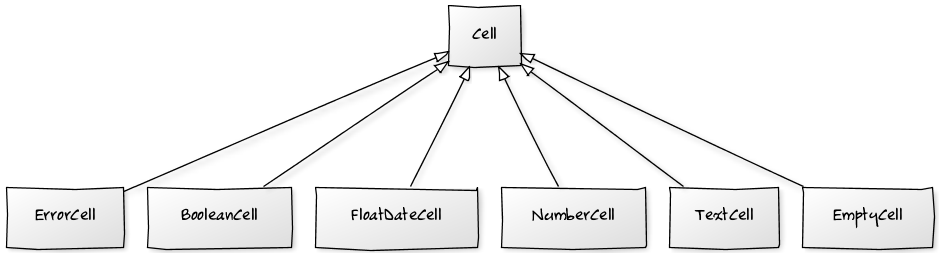
\includegraphics[width=6in]{cell.png}


\subsection{Circularity}
\label{cell:circularity}
Note that a Cell depends on a Workbook.

And a Workbook (via a Sheet and a Row) depends on a Cell.

In some languages, we'd be obligated to define interfaces so that these
two classes could depend on each other sensibly. In Python, however,
we don't need to create an elaborate web of dependencies.


\subsection{Overheads}
\label{cell:overheads}
Here are the module docstring and imports.

\begin{Verbatim}[commandchars=\\\{\}]
\PYG{l+s+sd}{\PYGZdq{}\PYGZdq{}\PYGZdq{}stingray.cell \PYGZhy{}\PYGZhy{} Defines Cell as the atomic data element in a sheet}
\PYG{l+s+sd}{of a workbook.}

\PYG{l+s+sd}{A cell has a value, it\PYGZsq{}s part of a workbook.}
\PYG{l+s+sd}{\PYGZdq{}\PYGZdq{}\PYGZdq{}}

\PYG{k+kn}{import} \PYG{n+nn}{locale}
\PYG{k+kn}{import} \PYG{n+nn}{decimal}
\PYG{k+kn}{import} \PYG{n+nn}{datetime}
\PYG{k+kn}{import} \PYG{n+nn}{time}
\PYG{k+kn}{from} \PYG{n+nn}{collections} \PYG{k+kn}{import} \PYG{n}{Hashable}
\end{Verbatim}

A version string.

\begin{Verbatim}[commandchars=\\\{\}]
\PYG{n}{\PYGZus{}\PYGZus{}version\PYGZus{}\PYGZus{}} \PYG{o}{=} \PYG{l+s}{\PYGZdq{}}\PYG{l+s}{4.4.6}\PYG{l+s}{\PYGZdq{}}
\end{Verbatim}

Just to be sure that any locale-based processing will actually
work, we establish a default locale.

\begin{Verbatim}[commandchars=\\\{\}]
\PYG{n}{locale}\PYG{o}{.}\PYG{n}{setlocale}\PYG{p}{(}\PYG{n}{locale}\PYG{o}{.}\PYG{n}{LC\PYGZus{}ALL}\PYG{p}{,} \PYG{l+s}{\PYGZsq{}}\PYG{l+s}{\PYGZsq{}}\PYG{p}{)}
\end{Verbatim}


\subsection{Cell}
\label{cell:cell}\index{Cell (class in cell)}

\begin{fulllineitems}
\phantomsection\label{cell:cell.Cell}\pysigline{\strong{class }\code{cell.}\bfcode{Cell}}
The {\hyperref[cell:cell.Cell]{\code{cell.Cell}}} class hierarchy extends this base class.  Note that we have
a relatively short list of built-in conversions.
For more complex, application-specific conversions, the raw {\hyperref[cell:cell.Cell.value]{\code{value}}} is available as a property.
\index{value (cell.Cell attribute)}

\begin{fulllineitems}
\phantomsection\label{cell:cell.Cell.value}\pysigline{\bfcode{value}}
The raw data, often a String from a workbook. May also be a
sequence of bytes for COBOL.

\end{fulllineitems}

\index{workbook (cell.Cell attribute)}

\begin{fulllineitems}
\phantomsection\label{cell:cell.Cell.workbook}\pysigline{\bfcode{workbook}}
The {\hyperref[workbook/base:workbook.base.Workbook]{\code{workbook.base.Workbook}}} that created this Cell.
This is largely used for Excel date conversions, but there
could be other context needs for lazy access to data.

\end{fulllineitems}


\end{fulllineitems}


\begin{Verbatim}[commandchars=\\\{\}]
\PYG{k}{class} \PYG{n+nc}{Cell}\PYG{p}{(} \PYG{n}{Hashable} \PYG{p}{)}\PYG{p}{:}
    \PYG{l+s+sd}{\PYGZdq{}\PYGZdq{}\PYGZdq{}A class hierarchy for each kind of Cell.}
\PYG{l+s+sd}{    \PYGZdq{}\PYGZdq{}\PYGZdq{}}
    \PYG{k}{def} \PYG{n+nf}{\PYGZus{}\PYGZus{}init\PYGZus{}\PYGZus{}}\PYG{p}{(} \PYG{n+nb+bp}{self}\PYG{p}{,} \PYG{n}{value}\PYG{o}{=}\PYG{n+nb+bp}{None}\PYG{p}{,} \PYG{n}{workbook}\PYG{o}{=}\PYG{n+nb+bp}{None} \PYG{p}{)}\PYG{p}{:}
        \PYG{l+s+sd}{\PYGZdq{}\PYGZdq{}\PYGZdq{}Build a new Cell; the atomic data element of a  workbook.}

\PYG{l+s+sd}{        :param value: Raw value, generally a string for most workbooks.}
\PYG{l+s+sd}{        :param workbook: Parent workbook, required for some}
\PYG{l+s+sd}{            conversions and for lazy access to data.}
\PYG{l+s+sd}{        \PYGZdq{}\PYGZdq{}\PYGZdq{}}
        \PYG{n+nb+bp}{self}\PYG{o}{.}\PYG{n}{\PYGZus{}value}\PYG{p}{,} \PYG{n+nb+bp}{self}\PYG{o}{.}\PYG{n}{workbook} \PYG{o}{=} \PYG{n}{value}\PYG{p}{,} \PYG{n}{workbook}
    \PYG{k}{def} \PYG{n+nf}{\PYGZus{}\PYGZus{}repr\PYGZus{}\PYGZus{}}\PYG{p}{(} \PYG{n+nb+bp}{self} \PYG{p}{)}\PYG{p}{:}
        \PYG{k}{return} \PYG{l+s}{\PYGZdq{}}\PYG{l+s}{\PYGZob{}0\PYGZcb{}(\PYGZob{}1!r\PYGZcb{})}\PYG{l+s}{\PYGZdq{}}\PYG{o}{.}\PYG{n}{format}\PYG{p}{(}
            \PYG{n+nb+bp}{self}\PYG{o}{.}\PYG{n}{\PYGZus{}\PYGZus{}class\PYGZus{}\PYGZus{}}\PYG{o}{.}\PYG{n}{\PYGZus{}\PYGZus{}name\PYGZus{}\PYGZus{}}\PYG{p}{,} \PYG{n+nb+bp}{self}\PYG{o}{.}\PYG{n}{\PYGZus{}value} \PYG{p}{)}
    \PYG{k}{def} \PYG{n+nf}{is\PYGZus{}empty}\PYG{p}{(} \PYG{n+nb+bp}{self} \PYG{p}{)}\PYG{p}{:}
        \PYG{k}{return} \PYG{n+nb+bp}{self}\PYG{o}{.}\PYG{n}{\PYGZus{}value} \PYG{o+ow}{is} \PYG{n+nb+bp}{None}
    \PYG{k}{def} \PYG{n+nf}{to\PYGZus{}int}\PYG{p}{(} \PYG{n+nb+bp}{self} \PYG{p}{)}\PYG{p}{:} \PYG{k}{return} \PYG{n+nb+bp}{NotImplemented}
    \PYG{k}{def} \PYG{n+nf}{to\PYGZus{}float}\PYG{p}{(} \PYG{n+nb+bp}{self} \PYG{p}{)}\PYG{p}{:} \PYG{k}{return} \PYG{n+nb+bp}{NotImplemented}
    \PYG{k}{def} \PYG{n+nf}{to\PYGZus{}decimal}\PYG{p}{(} \PYG{n+nb+bp}{self}\PYG{p}{,} \PYG{n}{digits}\PYG{o}{=}\PYG{n+nb+bp}{None} \PYG{p}{)}\PYG{p}{:} \PYG{k}{return} \PYG{n+nb+bp}{NotImplemented}
    \PYG{k}{def} \PYG{n+nf}{to\PYGZus{}str}\PYG{p}{(} \PYG{n+nb+bp}{self} \PYG{p}{)}\PYG{p}{:} \PYG{k}{return} \PYG{n+nb+bp}{NotImplemented}
    \PYG{k}{def} \PYG{n+nf}{to\PYGZus{}datetime}\PYG{p}{(} \PYG{n+nb+bp}{self}\PYG{p}{,} \PYG{n}{format}\PYG{o}{=}\PYG{n+nb+bp}{None} \PYG{p}{)}\PYG{p}{:} \PYG{k}{return} \PYG{n+nb+bp}{NotImplemented}
    \PYG{k}{def} \PYG{n+nf}{to\PYGZus{}digit\PYGZus{}str}\PYG{p}{(} \PYG{n+nb+bp}{self}\PYG{p}{,} \PYG{n+nb}{len}\PYG{o}{=}\PYG{l+m+mi}{5} \PYG{p}{)}\PYG{p}{:} \PYG{k}{return} \PYG{n+nb+bp}{NotImplemented}
\end{Verbatim}

One feature of a cell that's required when we do data profiling is to
create a usable hash from the cell class and raw data value.

\begin{Verbatim}[commandchars=\\\{\}]
\PYG{k}{def} \PYG{n+nf}{\PYGZus{}\PYGZus{}hash\PYGZus{}\PYGZus{}}\PYG{p}{(} \PYG{n+nb+bp}{self} \PYG{p}{)}\PYG{p}{:}
    \PYG{k}{return} \PYG{n+nb}{hash}\PYG{p}{(}\PYG{n+nb+bp}{self}\PYG{o}{.}\PYG{n}{\PYGZus{}value}\PYG{p}{)} \PYG{o}{\PYGZca{}} \PYG{n+nb}{hash}\PYG{p}{(}\PYG{n+nb+bp}{self}\PYG{o}{.}\PYG{n}{\PYGZus{}\PYGZus{}class\PYGZus{}\PYGZus{}}\PYG{p}{)}
\PYG{k}{def} \PYG{n+nf}{\PYGZus{}\PYGZus{}eq\PYGZus{}\PYGZus{}}\PYG{p}{(} \PYG{n+nb+bp}{self}\PYG{p}{,} \PYG{n}{other} \PYG{p}{)}\PYG{p}{:}
    \PYG{k}{return} \PYG{n+nb+bp}{self}\PYG{o}{.}\PYG{n}{\PYGZus{}\PYGZus{}class\PYGZus{}\PYGZus{}} \PYG{o}{==} \PYG{n}{other}\PYG{o}{.}\PYG{n}{\PYGZus{}\PYGZus{}class\PYGZus{}\PYGZus{}} \PYG{o+ow}{and} \PYG{n+nb+bp}{self}\PYG{o}{.}\PYG{n}{\PYGZus{}value} \PYG{o}{==} \PYG{n}{other}\PYG{o}{.}\PYG{n}{\PYGZus{}value}
\PYG{k}{def} \PYG{n+nf}{\PYGZus{}\PYGZus{}ne\PYGZus{}\PYGZus{}}\PYG{p}{(} \PYG{n+nb+bp}{self}\PYG{p}{,} \PYG{n}{other} \PYG{p}{)}\PYG{p}{:}
    \PYG{k}{return} \PYG{n+nb+bp}{self}\PYG{o}{.}\PYG{n}{\PYGZus{}\PYGZus{}class\PYGZus{}\PYGZus{}} \PYG{o}{!=} \PYG{n}{other}\PYG{o}{.}\PYG{n}{\PYGZus{}\PYGZus{}class\PYGZus{}\PYGZus{}} \PYG{o+ow}{or} \PYG{n+nb+bp}{self}\PYG{o}{.}\PYG{n}{\PYGZus{}value} \PYG{o}{!=} \PYG{n}{other}\PYG{o}{.}\PYG{n}{\PYGZus{}value}
\end{Verbatim}

We make a token effort at making a cell more-or-less immutable.  This makes it
hashable.

\begin{Verbatim}[commandchars=\\\{\}]
\PYG{n+nd}{@property}
\PYG{k}{def} \PYG{n+nf}{value}\PYG{p}{(} \PYG{n+nb+bp}{self} \PYG{p}{)}\PYG{p}{:}
    \PYG{k}{return} \PYG{n+nb+bp}{self}\PYG{o}{.}\PYG{n}{\PYGZus{}value}
\end{Verbatim}

\begin{notice}{note}{Todo}

Unit test cases for the hashable interface of Cell
\end{notice}


\subsection{EmptyCell}
\label{cell:emptycell}\index{EmptyCell (class in cell)}

\begin{fulllineitems}
\phantomsection\label{cell:cell.EmptyCell}\pysigline{\strong{class }\code{cell.}\bfcode{EmptyCell}}
An \code{EmptyCell} implements empty cells.  \code{xlrd} may report them as a type \code{XL\_CELL\_EMPTY}.
A Numbers spreadsheet may use the \code{\textless{}o\textgreater{}} or \code{\textless{}g\textgreater{}} tag.

\end{fulllineitems}


\begin{Verbatim}[commandchars=\\\{\}]
\PYG{k}{class} \PYG{n+nc}{EmptyCell}\PYG{p}{(} \PYG{n}{Cell} \PYG{p}{)}\PYG{p}{:}
    \PYG{l+s+sd}{\PYGZdq{}\PYGZdq{}\PYGZdq{}The *value* will be \PYGZsq{}\PYGZsq{}, but we ignore that.\PYGZdq{}\PYGZdq{}\PYGZdq{}}
    \PYG{k}{def} \PYG{n+nf}{is\PYGZus{}empty}\PYG{p}{(} \PYG{n+nb+bp}{self} \PYG{p}{)}\PYG{p}{:} \PYG{k}{return} \PYG{n+nb+bp}{True}
    \PYG{k}{def} \PYG{n+nf}{to\PYGZus{}int}\PYG{p}{(} \PYG{n+nb+bp}{self} \PYG{p}{)}\PYG{p}{:} \PYG{k}{return} \PYG{n+nb+bp}{None}
    \PYG{k}{def} \PYG{n+nf}{to\PYGZus{}float}\PYG{p}{(} \PYG{n+nb+bp}{self} \PYG{p}{)}\PYG{p}{:} \PYG{k}{return} \PYG{n+nb+bp}{None}
    \PYG{k}{def} \PYG{n+nf}{to\PYGZus{}decimal}\PYG{p}{(} \PYG{n+nb+bp}{self}\PYG{p}{,} \PYG{n}{digits}\PYG{o}{=}\PYG{n+nb+bp}{None} \PYG{p}{)}\PYG{p}{:} \PYG{k}{return} \PYG{n+nb+bp}{None}
    \PYG{k}{def} \PYG{n+nf}{to\PYGZus{}str}\PYG{p}{(} \PYG{n+nb+bp}{self} \PYG{p}{)}\PYG{p}{:} \PYG{k}{return} \PYG{n+nb+bp}{None}
    \PYG{k}{def} \PYG{n+nf}{to\PYGZus{}datetime}\PYG{p}{(} \PYG{n+nb+bp}{self}\PYG{p}{,} \PYG{n}{format}\PYG{o}{=}\PYG{n+nb+bp}{None} \PYG{p}{)}\PYG{p}{:} \PYG{k}{return} \PYG{n+nb+bp}{None}
    \PYG{k}{def} \PYG{n+nf}{to\PYGZus{}digit\PYGZus{}str}\PYG{p}{(} \PYG{n+nb+bp}{self}\PYG{p}{,} \PYG{n+nb}{len}\PYG{o}{=}\PYG{n+nb+bp}{None} \PYG{p}{)}\PYG{p}{:} \PYG{k}{return} \PYG{n+nb+bp}{None}
\end{Verbatim}


\subsection{TextCell}
\label{cell:textcell}\index{TextCell (class in cell)}

\begin{fulllineitems}
\phantomsection\label{cell:cell.TextCell}\pysigline{\strong{class }\code{cell.}\bfcode{TextCell}}
A \code{TextCell} implements the cells with text values.
\code{xlrd} may report them as a type \code{XL\_CELL\_TEXT}.
It's often possible to interpret the text as some other value,
so the conversions make reasonable attempts at that.

This is used for CSV workbooks as well as XLS workbooks.
This is the default type for Fixed format files, also.

Note that COBOL files will explicitly have bytes values, not
string values.

\end{fulllineitems}


\begin{Verbatim}[commandchars=\\\{\}]
\PYG{k}{class} \PYG{n+nc}{TextCell}\PYG{p}{(} \PYG{n}{Cell} \PYG{p}{)}\PYG{p}{:}
    \PYG{l+s+sd}{\PYGZdq{}\PYGZdq{}\PYGZdq{}A Cell which contains a Python string value.\PYGZdq{}\PYGZdq{}\PYGZdq{}}
    \PYG{k}{def} \PYG{n+nf}{to\PYGZus{}int}\PYG{p}{(} \PYG{n+nb+bp}{self} \PYG{p}{)}\PYG{p}{:}
        \PYG{k}{return} \PYG{n+nb}{int}\PYG{p}{(} \PYG{n+nb+bp}{self}\PYG{o}{.}\PYG{n}{value} \PYG{p}{)}
    \PYG{k}{def} \PYG{n+nf}{to\PYGZus{}float}\PYG{p}{(} \PYG{n+nb+bp}{self} \PYG{p}{)}\PYG{p}{:}
        \PYG{k}{return} \PYG{n+nb}{float}\PYG{p}{(} \PYG{n+nb+bp}{self}\PYG{o}{.}\PYG{n}{value} \PYG{p}{)}
    \PYG{k}{def} \PYG{n+nf}{to\PYGZus{}decimal}\PYG{p}{(} \PYG{n+nb+bp}{self}\PYG{p}{,} \PYG{n}{digits}\PYG{o}{=}\PYG{l+m+mi}{0} \PYG{p}{)}\PYG{p}{:}
        \PYG{k}{return} \PYG{n}{decimal}\PYG{o}{.}\PYG{n}{Decimal}\PYG{p}{(} \PYG{n+nb+bp}{self}\PYG{o}{.}\PYG{n}{value} \PYG{p}{)}
    \PYG{k}{def} \PYG{n+nf}{to\PYGZus{}str}\PYG{p}{(} \PYG{n+nb+bp}{self} \PYG{p}{)}\PYG{p}{:}
        \PYG{k}{return} \PYG{n+nb+bp}{self}\PYG{o}{.}\PYG{n}{value}
    \PYG{k}{def} \PYG{n+nf}{to\PYGZus{}datetime}\PYG{p}{(} \PYG{n+nb+bp}{self}\PYG{p}{,} \PYG{n}{format}\PYG{o}{=}\PYG{n+nb+bp}{None} \PYG{p}{)}\PYG{p}{:}
        \PYG{k}{if} \PYG{n}{format} \PYG{o+ow}{is} \PYG{n+nb+bp}{None}\PYG{p}{:}
            \PYG{k}{try}\PYG{p}{:}
                \PYG{n}{format} \PYG{o}{=} \PYG{n}{locale}\PYG{o}{.}\PYG{n}{nl\PYGZus{}langinfo}\PYG{p}{(}\PYG{n}{locale}\PYG{o}{.}\PYG{n}{D\PYGZus{}FMT}\PYG{p}{)}
            \PYG{k}{except} \PYG{n+ne}{AttributeError} \PYG{k}{as} \PYG{n}{e}\PYG{p}{:}
                \PYG{c}{\PYGZsh{} Windows}
                \PYG{n}{format} \PYG{o}{=} \PYG{l+s}{\PYGZdq{}}\PYG{l+s+si}{\PYGZpc{}x}\PYG{l+s}{\PYGZdq{}}
        \PYG{k}{return} \PYG{n}{datetime}\PYG{o}{.}\PYG{n}{datetime}\PYG{o}{.}\PYG{n}{strptime}\PYG{p}{(}\PYG{n+nb+bp}{self}\PYG{o}{.}\PYG{n}{value}\PYG{p}{,}\PYG{n}{format}\PYG{p}{)}
    \PYG{k}{def} \PYG{n+nf}{to\PYGZus{}digit\PYGZus{}str}\PYG{p}{(} \PYG{n+nb+bp}{self}\PYG{p}{,} \PYG{n}{length}\PYG{o}{=}\PYG{l+m+mi}{5} \PYG{p}{)}\PYG{p}{:}
        \PYG{n}{txt}\PYG{o}{=} \PYG{l+s}{\PYGZdq{}}\PYG{l+s}{\PYGZob{}0:0\PYGZgt{}\PYGZob{}length\PYGZcb{}d\PYGZcb{}}\PYG{l+s}{\PYGZdq{}}\PYG{o}{.}\PYG{n}{format}\PYG{p}{(}\PYG{n+nb}{int}\PYG{p}{(}\PYG{n+nb+bp}{self}\PYG{o}{.}\PYG{n}{value}\PYG{p}{)}\PYG{p}{,} \PYG{n}{length}\PYG{o}{=}\PYG{n}{length}\PYG{p}{)}
        \PYG{k}{return} \PYG{n}{txt}
\end{Verbatim}


\subsection{NumberCell}
\label{cell:numbercell}\index{NumberCell (class in cell)}

\begin{fulllineitems}
\phantomsection\label{cell:cell.NumberCell}\pysigline{\strong{class }\code{cell.}\bfcode{NumberCell}}
A \code{NumberCell} implements the cells with a float value.
\code{xlrd} may report them as a type \code{XL\_CELL\_NUMBER}.
A variety of conversions make sense for a number value.

\end{fulllineitems}


\begin{Verbatim}[commandchars=\\\{\}]
\PYG{k}{class} \PYG{n+nc}{NumberCell}\PYG{p}{(} \PYG{n}{Cell} \PYG{p}{)}\PYG{p}{:}
    \PYG{l+s+sd}{\PYGZdq{}\PYGZdq{}\PYGZdq{}A cell which contains a Python float value.\PYGZdq{}\PYGZdq{}\PYGZdq{}}
    \PYG{k}{def} \PYG{n+nf}{to\PYGZus{}int}\PYG{p}{(} \PYG{n+nb+bp}{self} \PYG{p}{)}\PYG{p}{:}
        \PYG{k}{return} \PYG{n+nb}{int}\PYG{p}{(} \PYG{n+nb+bp}{self}\PYG{o}{.}\PYG{n}{value} \PYG{p}{)}
    \PYG{k}{def} \PYG{n+nf}{to\PYGZus{}float}\PYG{p}{(} \PYG{n+nb+bp}{self} \PYG{p}{)}\PYG{p}{:}
        \PYG{k}{if} \PYG{n+nb}{isinstance}\PYG{p}{(}\PYG{n+nb+bp}{self}\PYG{o}{.}\PYG{n}{value}\PYG{p}{,}\PYG{n+nb}{float}\PYG{p}{)}\PYG{p}{:}
            \PYG{k}{return} \PYG{n+nb+bp}{self}\PYG{o}{.}\PYG{n}{value}
        \PYG{c}{\PYGZsh{} likely, it\PYGZsq{}s Decimal!}
        \PYG{k}{return} \PYG{n+nb}{float}\PYG{p}{(}\PYG{n+nb+bp}{self}\PYG{o}{.}\PYG{n}{value}\PYG{p}{)}
    \PYG{k}{def} \PYG{n+nf}{to\PYGZus{}decimal}\PYG{p}{(} \PYG{n+nb+bp}{self}\PYG{p}{,} \PYG{n}{digits}\PYG{o}{=}\PYG{l+m+mi}{0} \PYG{p}{)}\PYG{p}{:}
        \PYG{k}{if} \PYG{n+nb}{isinstance}\PYG{p}{(}\PYG{n+nb+bp}{self}\PYG{o}{.}\PYG{n}{value}\PYG{p}{,}\PYG{n+nb}{float}\PYG{p}{)}\PYG{p}{:}
            \PYG{n}{fmt}\PYG{o}{=} \PYG{l+s}{\PYGZdq{}}\PYG{l+s}{\PYGZob{}0:0.\PYGZob{}digits\PYGZcb{}f\PYGZcb{}}\PYG{l+s}{\PYGZdq{}}
            \PYG{k}{return} \PYG{n}{decimal}\PYG{o}{.}\PYG{n}{Decimal}\PYG{p}{(} \PYG{n}{fmt}\PYG{o}{.}\PYG{n}{format}\PYG{p}{(}\PYG{n+nb+bp}{self}\PYG{o}{.}\PYG{n}{value}\PYG{p}{,} \PYG{n}{digits}\PYG{o}{=}\PYG{n}{digits}\PYG{p}{)} \PYG{p}{)}
        \PYG{k}{elif} \PYG{n+nb}{isinstance}\PYG{p}{(}\PYG{n+nb+bp}{self}\PYG{o}{.}\PYG{n}{value}\PYG{p}{,}\PYG{n}{decimal}\PYG{o}{.}\PYG{n}{Decimal}\PYG{p}{)}\PYG{p}{:}
            \PYG{k}{return} \PYG{n+nb+bp}{self}\PYG{o}{.}\PYG{n}{value}
        \PYG{k}{else}\PYG{p}{:}
            \PYG{k}{return} \PYG{n}{decimal}\PYG{o}{.}\PYG{n}{Decimal}\PYG{p}{(}\PYG{n+nb+bp}{self}\PYG{o}{.}\PYG{n}{value}\PYG{p}{)}
    \PYG{k}{def} \PYG{n+nf}{to\PYGZus{}str}\PYG{p}{(} \PYG{n+nb+bp}{self} \PYG{p}{)}\PYG{p}{:}
        \PYG{k}{return} \PYG{n+nb}{str}\PYG{p}{(}\PYG{n+nb+bp}{self}\PYG{o}{.}\PYG{n}{value}\PYG{p}{)}
    \PYG{k}{def} \PYG{n+nf}{to\PYGZus{}datetime}\PYG{p}{(} \PYG{n+nb+bp}{self}\PYG{p}{,} \PYG{n}{format}\PYG{o}{=}\PYG{n+nb+bp}{None} \PYG{p}{)}\PYG{p}{:}
        \PYG{k}{assert} \PYG{n}{format} \PYG{o+ow}{is} \PYG{n+nb+bp}{None}\PYG{p}{,} \PYG{l+s}{\PYGZdq{}}\PYG{l+s}{Format is not used.}\PYG{l+s}{\PYGZdq{}}

        \PYG{k}{return} \PYG{n+nb+bp}{self}\PYG{o}{.}\PYG{n}{workbook}\PYG{o}{.}\PYG{n}{float\PYGZus{}to\PYGZus{}date}\PYG{p}{(}\PYG{n+nb+bp}{self}\PYG{o}{.}\PYG{n}{value}\PYG{p}{)}

        \PYG{c}{\PYGZsh{}try:}
        \PYG{c}{\PYGZsh{}    dt= xlrd.xldate\PYGZus{}as\PYGZus{}tuple(self.value, self.workbook.datemode)}
        \PYG{c}{\PYGZsh{}except xlrd.xldate.XLDateAmbiguous as e:}
        \PYG{c}{\PYGZsh{}    ex= ValueError( \PYGZdq{}Ambiguous Date: \PYGZob{}0\PYGZcb{}\PYGZdq{}.format(self.value) )}
        \PYG{c}{\PYGZsh{}    raise ex from e}
        \PYG{c}{\PYGZsh{}return datetime.datetime(*dt)}

    \PYG{k}{def} \PYG{n+nf}{to\PYGZus{}digit\PYGZus{}str}\PYG{p}{(} \PYG{n+nb+bp}{self}\PYG{p}{,} \PYG{n}{length}\PYG{o}{=}\PYG{l+m+mi}{5} \PYG{p}{)}\PYG{p}{:}
        \PYG{n}{txt}\PYG{o}{=} \PYG{l+s}{\PYGZdq{}}\PYG{l+s}{\PYGZob{}0:0\PYGZgt{}\PYGZob{}length\PYGZcb{}d\PYGZcb{}}\PYG{l+s}{\PYGZdq{}}\PYG{o}{.}\PYG{n}{format}\PYG{p}{(}\PYG{n+nb}{int}\PYG{p}{(}\PYG{n+nb+bp}{self}\PYG{o}{.}\PYG{n}{value}\PYG{p}{)}\PYG{p}{,} \PYG{n}{length}\PYG{o}{=}\PYG{n}{length}\PYG{p}{)}
        \PYG{k}{return} \PYG{n}{txt}
\end{Verbatim}


\subsection{FloatDateCell}
\label{cell:floatdatecell}\index{FloatDateCell (class in cell)}

\begin{fulllineitems}
\phantomsection\label{cell:cell.FloatDateCell}\pysigline{\strong{class }\code{cell.}\bfcode{FloatDateCell}}
A \code{FloatDateCell} implements the cells with \code{XL\_CELL\_DATE}.
Since the conversions are all identical to number,
we simply inherit the features of a number.

\end{fulllineitems}


\begin{Verbatim}[commandchars=\\\{\}]
\PYG{k}{class} \PYG{n+nc}{FloatDateCell}\PYG{p}{(} \PYG{n}{NumberCell} \PYG{p}{)}\PYG{p}{:}
    \PYG{l+s+sd}{\PYGZdq{}\PYGZdq{}\PYGZdq{}A cell which contains a float value that is actually an Excel date.\PYGZdq{}\PYGZdq{}\PYGZdq{}}
    \PYG{k}{pass}
\end{Verbatim}

Other formats have other kinds of date cells that aren't simply
dressed-up floating-point numbers.


\subsection{BooleanCell}
\label{cell:booleancell}\index{BooleanCell (class in cell)}

\begin{fulllineitems}
\phantomsection\label{cell:cell.BooleanCell}\pysigline{\strong{class }\code{cell.}\bfcode{BooleanCell}}
A \code{BooleanCell} implements the cells with \code{XL\_CELL\_BOOLEAN}.
Since the conversions are all identical to number,
we simply inherit the features.

\end{fulllineitems}


\begin{Verbatim}[commandchars=\\\{\}]
\PYG{k}{class} \PYG{n+nc}{BooleanCell}\PYG{p}{(} \PYG{n}{NumberCell} \PYG{p}{)}\PYG{p}{:}
    \PYG{l+s+sd}{\PYGZdq{}\PYGZdq{}\PYGZdq{}A cell which contains a boolean value.\PYGZdq{}\PYGZdq{}\PYGZdq{}}
    \PYG{k}{pass}
\end{Verbatim}


\subsection{ErrorCell}
\label{cell:errorcell}\index{ErrorCell (class in cell)}

\begin{fulllineitems}
\phantomsection\label{cell:cell.ErrorCell}\pysigline{\strong{class }\code{cell.}\bfcode{ErrorCell}}
An \code{ErrorCell} implements the cells with \code{XL\_CELL\_ERROR}.
The only sensible conversion is \code{ErrorCell.to\_str()} which reports
the error string for the cell.

\end{fulllineitems}


\begin{Verbatim}[commandchars=\\\{\}]
\PYG{k}{class} \PYG{n+nc}{ErrorCell}\PYG{p}{(} \PYG{n}{Cell} \PYG{p}{)}\PYG{p}{:}
    \PYG{l+s+sd}{\PYGZdq{}\PYGZdq{}\PYGZdq{}A cell which contains an error code.\PYGZdq{}\PYGZdq{}\PYGZdq{}}
    \PYG{k}{def} \PYG{n+nf}{to\PYGZus{}int}\PYG{p}{(} \PYG{n+nb+bp}{self} \PYG{p}{)}\PYG{p}{:}
        \PYG{k}{raise} \PYG{n+ne}{ValueError}\PYG{p}{(} \PYG{n+nb+bp}{self}\PYG{o}{.}\PYG{n}{value} \PYG{p}{)}
    \PYG{k}{def} \PYG{n+nf}{to\PYGZus{}float}\PYG{p}{(} \PYG{n+nb+bp}{self} \PYG{p}{)}\PYG{p}{:}
        \PYG{k}{raise} \PYG{n+ne}{ValueError}\PYG{p}{(} \PYG{n+nb+bp}{self}\PYG{o}{.}\PYG{n}{value} \PYG{p}{)}
    \PYG{k}{def} \PYG{n+nf}{to\PYGZus{}decimal}\PYG{p}{(} \PYG{n+nb+bp}{self}\PYG{p}{,} \PYG{n}{digits}\PYG{o}{=}\PYG{l+m+mi}{0} \PYG{p}{)}\PYG{p}{:}
        \PYG{k}{raise} \PYG{n+ne}{ValueError}\PYG{p}{(} \PYG{n+nb+bp}{self}\PYG{o}{.}\PYG{n}{value} \PYG{p}{)}
    \PYG{k}{def} \PYG{n+nf}{to\PYGZus{}str}\PYG{p}{(} \PYG{n+nb+bp}{self} \PYG{p}{)}\PYG{p}{:}
        \PYG{k}{return} \PYG{n+nb+bp}{self}\PYG{o}{.}\PYG{n}{value}
    \PYG{k}{def} \PYG{n+nf}{to\PYGZus{}datetime}\PYG{p}{(} \PYG{n+nb+bp}{self}\PYG{p}{,} \PYG{n}{format}\PYG{o}{=}\PYG{n+nb+bp}{None} \PYG{p}{)}\PYG{p}{:}
        \PYG{k}{raise} \PYG{n+ne}{ValueError}\PYG{p}{(} \PYG{n+nb+bp}{self}\PYG{o}{.}\PYG{n}{value} \PYG{p}{)}
    \PYG{k}{def} \PYG{n+nf}{to\PYGZus{}digit\PYGZus{}str}\PYG{p}{(} \PYG{n+nb+bp}{self}\PYG{p}{,} \PYG{n}{length}\PYG{o}{=}\PYG{l+m+mi}{5} \PYG{p}{)}\PYG{p}{:}
        \PYG{k}{raise} \PYG{n+ne}{ValueError}\PYG{p}{(} \PYG{n+nb+bp}{self}\PYG{o}{.}\PYG{n}{value} \PYG{p}{)}
\end{Verbatim}


\subsection{DateCell}
\label{cell:datecell}\index{DateCell (class in cell)}

\begin{fulllineitems}
\phantomsection\label{cell:cell.DateCell}\pysigline{\strong{class }\code{cell.}\bfcode{DateCell}}
A \code{DateCell} implements a cell with a proper date-time value.
This is a value which did not come from a workbook float value.

This could be a parsed string, for example.

A variety of conversions make sense for a proper date value.

\end{fulllineitems}


\begin{Verbatim}[commandchars=\\\{\}]
\PYG{k}{class} \PYG{n+nc}{DateCell}\PYG{p}{(} \PYG{n}{Cell} \PYG{p}{)}\PYG{p}{:}
    \PYG{l+s+sd}{\PYGZdq{}\PYGZdq{}\PYGZdq{}A cell which contains a proper :py:mod:{}`datetime{}` value.\PYGZdq{}\PYGZdq{}\PYGZdq{}}
    \PYG{k}{def} \PYG{n+nf}{to\PYGZus{}int}\PYG{p}{(} \PYG{n+nb+bp}{self} \PYG{p}{)}\PYG{p}{:}
        \PYG{k}{return} \PYG{n+nb}{int}\PYG{p}{(}\PYG{n+nb+bp}{self}\PYG{o}{.}\PYG{n}{to\PYGZus{}float}\PYG{p}{(}\PYG{p}{)}\PYG{p}{)}
    \PYG{k}{def} \PYG{n+nf}{to\PYGZus{}float}\PYG{p}{(} \PYG{n+nb+bp}{self} \PYG{p}{)}\PYG{p}{:}

        \PYG{k}{return} \PYG{n+nb+bp}{self}\PYG{o}{.}\PYG{n}{workbook}\PYG{o}{.}\PYG{n}{date\PYGZus{}to\PYGZus{}float}\PYG{p}{(}\PYG{n+nb+bp}{self}\PYG{o}{.}\PYG{n}{value}\PYG{p}{)}

        \PYG{c}{\PYGZsh{}timetuple= self.value.timetuple()[:6]}
        \PYG{c}{\PYGZsh{}xl= xlrd.xldate.xldate\PYGZus{}from\PYGZus{}datetime\PYGZus{}tuple(}
        \PYG{c}{\PYGZsh{}    timetuple,}
        \PYG{c}{\PYGZsh{}    self.workbook.datemode)}
        \PYG{c}{\PYGZsh{}return xl}

    \PYG{k}{def} \PYG{n+nf}{to\PYGZus{}decimal}\PYG{p}{(} \PYG{n+nb+bp}{self}\PYG{p}{,} \PYG{n}{digits}\PYG{o}{=}\PYG{l+m+mi}{0} \PYG{p}{)}\PYG{p}{:}
        \PYG{n}{fmt}\PYG{o}{=} \PYG{l+s}{\PYGZdq{}}\PYG{l+s}{\PYGZob{}0:0.\PYGZob{}digits\PYGZcb{}f\PYGZcb{}}\PYG{l+s}{\PYGZdq{}}
        \PYG{k}{return} \PYG{n}{decimal}\PYG{o}{.}\PYG{n}{Decimal}\PYG{p}{(} \PYG{n}{fmt}\PYG{o}{.}\PYG{n}{format}\PYG{p}{(}\PYG{n+nb+bp}{self}\PYG{o}{.}\PYG{n}{to\PYGZus{}float}\PYG{p}{(}\PYG{p}{)}\PYG{p}{,}\PYG{n}{digits}\PYG{o}{=}\PYG{n}{digits}\PYG{p}{)} \PYG{p}{)}
    \PYG{k}{def} \PYG{n+nf}{to\PYGZus{}str}\PYG{p}{(} \PYG{n+nb+bp}{self} \PYG{p}{)}\PYG{p}{:}
        \PYG{k}{return} \PYG{n+nb}{str}\PYG{p}{(}\PYG{n+nb+bp}{self}\PYG{o}{.}\PYG{n}{value}\PYG{p}{)}
    \PYG{k}{def} \PYG{n+nf}{to\PYGZus{}datetime}\PYG{p}{(} \PYG{n+nb+bp}{self}\PYG{p}{,} \PYG{n}{format}\PYG{o}{=}\PYG{n+nb+bp}{None} \PYG{p}{)}\PYG{p}{:}
        \PYG{k}{return} \PYG{n+nb+bp}{self}\PYG{o}{.}\PYG{n}{value}
    \PYG{k}{def} \PYG{n+nf}{to\PYGZus{}digit\PYGZus{}str}\PYG{p}{(} \PYG{n+nb+bp}{self}\PYG{p}{,} \PYG{n}{length}\PYG{o}{=}\PYG{l+m+mi}{5} \PYG{p}{)}\PYG{p}{:}
        \PYG{n}{fmt}\PYG{o}{=} \PYG{l+s}{\PYGZdq{}}\PYG{l+s}{\PYGZob{}\PYGZob{}0:0\PYGZgt{}\PYGZob{}0\PYGZcb{}d\PYGZcb{}\PYGZcb{}}\PYG{l+s}{\PYGZdq{}}\PYG{o}{.}\PYG{n}{format}\PYG{p}{(}\PYG{n}{length}\PYG{p}{)}
        \PYG{k}{return} \PYG{n}{fmt}\PYG{o}{.}\PYG{n}{format}\PYG{p}{(} \PYG{n+nb+bp}{self}\PYG{o}{.}\PYG{n}{to\PYGZus{}int}\PYG{p}{(}\PYG{p}{)} \PYG{p}{)}
\end{Verbatim}

For Apple Nnumbers, the \code{\textless{}d\textgreater{}} cells have a native date format.
This is a unique feature, since \code{xlrd}, XLSX and ODS don't have a
proper date cell value.


\subsection{Conversion Functions}
\label{cell:conversion-functions}
\begin{notice}{note}{Todo}

Refactor these into the {\hyperref[schema:module-schema]{\code{schema}}} module.

These functions are used to define schema, not process Cell objects \emph{per se}.
\end{notice}

The idea here is to create some functions that can be used to build
Schema attributes that handle proper date conversions.
\index{date\_from\_string() (in module cell)}

\begin{fulllineitems}
\phantomsection\label{cell:cell.date_from_string}\pysiglinewithargsret{\code{cell.}\bfcode{date\_from\_string}}{\emph{format}}{}
A closure based on a format string
that returns a single-argument conversion function.
\begin{quote}\begin{description}
\item[{Parameters}] \leavevmode
\textbf{format} -- the format string to use.

\end{description}\end{quote}

\end{fulllineitems}


\begin{Verbatim}[commandchars=\\\{\}]
\PYG{k}{def} \PYG{n+nf}{date\PYGZus{}from\PYGZus{}string}\PYG{p}{(} \PYG{n}{format} \PYG{p}{)}\PYG{p}{:}
    \PYG{k}{def} \PYG{n+nf}{the\PYGZus{}conversion}\PYG{p}{(} \PYG{n}{string} \PYG{p}{)}\PYG{p}{:}
        \PYG{k}{return} \PYG{n}{datetime}\PYG{o}{.}\PYG{n}{datetime}\PYG{o}{.}\PYG{n}{strptime}\PYG{p}{(} \PYG{n}{string}\PYG{p}{,} \PYG{n}{format} \PYG{p}{)}
    \PYG{k}{return} \PYG{n}{the\PYGZus{}conversion}
\end{Verbatim}

This forms a factory for the {\hyperref[cell:cell.DateCell]{\code{cell.DateCell}}} class.
\index{datecell\_from\_string() (in module cell)}

\begin{fulllineitems}
\phantomsection\label{cell:cell.datecell_from_string}\pysiglinewithargsret{\code{cell.}\bfcode{datecell\_from\_string}}{\emph{format}}{}
A closure based on a format string
that returns a single-argument conversion function.
\begin{quote}\begin{description}
\item[{Parameters}] \leavevmode
\textbf{format} -- the format string to use.

\end{description}\end{quote}

\end{fulllineitems}


\begin{Verbatim}[commandchars=\\\{\}]
\PYG{k}{def} \PYG{n+nf}{datecell\PYGZus{}from\PYGZus{}string}\PYG{p}{(} \PYG{n}{format} \PYG{p}{)}\PYG{p}{:}
    \PYG{n}{dt\PYGZus{}conv}\PYG{o}{=} \PYG{n}{date\PYGZus{}from\PYGZus{}string}\PYG{p}{(} \PYG{n}{format} \PYG{p}{)}
    \PYG{k}{def} \PYG{n+nf}{the\PYGZus{}conversion}\PYG{p}{(} \PYG{n}{string}\PYG{p}{,} \PYG{n}{workbook} \PYG{p}{)}\PYG{p}{:}
        \PYG{k}{return} \PYG{n}{DateCell}\PYG{p}{(} \PYG{n}{dt\PYGZus{}conv}\PYG{p}{(} \PYG{n}{string} \PYG{p}{)}\PYG{p}{,} \PYG{n}{workbook} \PYG{p}{)}
    \PYG{k}{return} \PYG{n}{the\PYGZus{}conversion}
\end{Verbatim}

This could be used like this in a schema definition.
\begin{alltt}
d = Attribute( name=''mm-dd-yy'', size=\emph{n}, offset=\emph{m},
    create=stingray.cell.datecell\_from\_string(``\%m/\%d/\%y'') )
\end{alltt}
\index{date\_from\_float() (in module cell)}

\begin{fulllineitems}
\phantomsection\label{cell:cell.date_from_float}\pysiglinewithargsret{\code{cell.}\bfcode{date\_from\_float}}{\emph{workbook}}{}
A closure based on an XLS workbook's datemode setting
that returns a single-argument conversion function.
\begin{quote}\begin{description}
\item[{Parameters}] \leavevmode
\textbf{workbook} -- the xlrd workbook with the required datemode.

\end{description}\end{quote}

\end{fulllineitems}


\begin{Verbatim}[commandchars=\\\{\}]
\PYG{k}{def} \PYG{n+nf}{date\PYGZus{}from\PYGZus{}float}\PYG{p}{(}\PYG{n}{workbook}\PYG{p}{)}\PYG{p}{:}
    \PYG{k}{return} \PYG{n}{workbook}\PYG{o}{.}\PYG{n}{float\PYGZus{}to\PYGZus{}date}
\end{Verbatim}

Once the definition of this was somewhat more complex. It was dependent on
\code{xlrd}; We've refactored it out of here to isolate all \code{xlrd}
dependencies properly.
\begin{alltt}
def date\_from\_float( workbook ):
    def the\_conversion( value ):
        try:
            dt= xlrd.xldate\_as\_tuple(value, workbook.datemode)
        except xlrd.xldate.XLDateAmbiguous as e:
            ex= ValueError( ``Ambiguous Date: \{0!r\}''.format(value) )
            raise ex from e
        return datetime.datetime(*dt)
    return the\_conversion
\end{alltt}

This function can be used to convert a raw float to a more useful
{\hyperref[cell:cell.DateCell]{\code{cell.DateCell}}} instance. This is only sensible in the XLRD context
where dates have peculiar conversion rules.
\begin{alltt}
float2date= stingray.cell.date\_from\_float(workbook)
d = Attribute( name=''mm-dd-yy'', size=\emph{n}, offset=\emph{m},
    create=lambda x, w: stingray.cell.DateCell( float2date(x), w ) )
\end{alltt}


\section{Sheet Module -- Sheet and Row Access}
\label{sheet:module-sheet}\label{sheet:sheet-module-sheet-and-row-access}\label{sheet:sheets}\label{sheet::doc}\index{sheet (module)}
A \emph{Sheet} is a generator
of \emph{Row} objects.  A \emph{Row} is a sequence of {\hyperref[cell:cell.Cell]{\code{cell.Cell}}} instances,
identified by position within the row.

We have three variations on {\hyperref[sheet:sheet.Sheet]{\code{sheet.Sheet}}}.
\begin{itemize}
\item {} 
A simple {\hyperref[sheet:sheet.Sheet]{\code{sheet.Sheet}}}  lacks a schema.
(This corresponds with \code{csv.reader()}.)
For workbooks with a well-known physical format, the schema can be optional.
Each {\hyperref[sheet:sheet.Row]{\code{sheet.Row}}} object can be built eagerly and accessed
by position.

\item {} 
A sheet with a schema.  There are two variations.
\begin{itemize}
\item {} 
{\hyperref[sheet:sheet.EmbeddedSchemaSheet]{\code{sheet.EmbeddedSchemaSheet}}} contains a schema.
This could be a simple as column titles in the first row.
(This corresponds to \code{csv.DictReader}.)
Or it could be considerably more complex.

\item {} 
{\hyperref[sheet:sheet.ExternalSchemaSheet]{\code{sheet.ExternalSchemaSheet}}} requires an external schema.
This schema may be simply a list of column titles supplied externally.
More often, the schema is a complete physical format description for
Fixed or COBOL format files.

\end{itemize}

\end{itemize}

A known physical format (like a workbook) can build {\hyperref[sheet:sheet.Row]{\code{sheet.Row}}} objects eagerly with or without a schema.
In the case of COBOL and fixed-format files, however, a {\hyperref[sheet:sheet.Row]{\code{sheet.Row}}}
cannot be built eagerly.  It must be a lazy
object which only builds {\hyperref[cell:cell.Cell]{\code{cell.Cell}}} as needed.
See {\hyperref[cobol:cobol]{\emph{The COBOL Package}}} for details.


\subsection{Get Embedded Schema Use Case}
\label{sheet:get-embedded-schema-use-case}
For an {\hyperref[sheet:sheet.EmbeddedSchemaSheet]{\code{sheet.EmbeddedSchemaSheet}}}, the application (or Workbook) must
do a three-step dance to get the data using schema that is embedded in the sheet.
\begin{enumerate}
\item {} 
Build a {\hyperref[sheet:sheet.EmbeddedSchemaSheet]{\code{sheet.EmbeddedSchemaSheet}}} with an
``embedded schema loader'' class.  (For example, {\hyperref[schema_loader:schema.loader.HeadingRowSchemaLoader]{\code{schema.loader.HeadingRowSchemaLoader}}}.)
The loader partitions rows into two sets: header and data.

\item {} 
Load the schema from the sheet.
The {\hyperref[sheet:sheet.Sheet]{\code{sheet.Sheet}}} will build an object of the loader class and use it to
gather the schema information.
The schema loading may involve skipping irrelevant rows or
combining multi-line headings or anything else required to parse the schema.

\item {} 
Get the rows from the sheet.
This will, also, invoke the attached loader to filter rows so that the header is not seen as data.

\end{enumerate}

The code might look like this:
\begin{alltt}
with \emph{open} as wb:
    sheet = EmbeddedSchemaSheet( workbook, `Sheet1', HeadingRowSchemaLoader )
    counts= process\_sheet( sheet )
    pprint.pprint( counts )
\end{alltt}

The idea is to simply access a sheet with column titles, no matter how complex
the column titles turn out to be.


\subsection{Get External Schema Use Case}
\label{sheet:get-external-schema-use-case}
For an {\hyperref[sheet:sheet.ExternalSchemaSheet]{\code{sheet.ExternalSchemaSheet}}}, the application (or Workbook)
must do a four-step dance to get data using schema.
\begin{enumerate}
\item {} 
Build a {\hyperref[schema_loader:schema.loader.ExternalSchemaLoader]{\code{schema.loader.ExternalSchemaLoader}}} as a schema loader.
This loader will require a source workbook, sheet name and a reader object.

\item {} 
Get the Schema object from the loader.

\item {} 
Build a {\hyperref[sheet:sheet.ExternalSchemaSheet]{\code{sheet.ExternalSchemaSheet}}} with the Schema object.

\item {} 
Get the rows from the sheet.

\end{enumerate}

And yes, the external source, is another
spreadsheet!  Worse, the external source could be a fixed file or workbook
for which a meta-schema is required to read the schema.

The code might look like this:
\begin{alltt}
with \emph{open schema} as swb:
    esl = ExternalSchemaLoader( swb, sheet\_name='Schema' )
    schema = esl.load()
with \emph{open data} as wb:
    sheet = ExternalSchemaSheet( wb, `Sheet1', schema )
    counts= process\_sheet( sheet )
    pprint.pprint( counts )
\end{alltt}

The idea is to get a schema and then use the schema to access data.


\subsection{Get Rows Use Case}
\label{sheet:get-rows-use-case}
The essential job of a {\hyperref[sheet:sheet.Sheet]{\code{sheet.Sheet}}} is to produce {\hyperref[sheet:sheet.Row]{\code{sheet.Row}}} instances.
A row is a sequence of {\hyperref[cell:cell.Cell]{\code{cell.Cell}}} instances.

Note that \code{csv} is eager about building a row from the source data.
This isn't universally appropriate.  COBOL files require lazy construction
of the row's cells.

A {\hyperref[schema:schema.Schema]{\code{schema.Schema}}} can transform a sequence row into a dictionary row
or a named tuple row.
The {\hyperref[schema:schema.Attribute.name]{\code{schema.Attribute.name}}} becomes the key for this row-as-dictionary.

We specifically delegate the row-as-dictionary interpretation to the {\hyperref[schema:schema.Schema]{\code{schema.Schema}}},
and avoid doing it in the {\hyperref[sheet:sheet.Sheet]{\code{sheet.Sheet}}}.  This is because most
workbook schemata are flat.  However, a COBOL schema can have a very complex
structure, making the row-as-dictionary too simplistic to be useful.

As noted above, there are two candidate implementations of a Row.
\begin{itemize}
\item {} 
\textbf{Eager}.  Appropriate for most (but not all) Physical Formats.  The
idea is to apply the schema immediately to create the row as a
tuple of cells.  \code{csv} does this, and it can be applied to
other workbook formats.  It can be applied to simple, flat
Fixed format files.

\item {} 
\textbf{Lazy}.  This is more appropriate for Fixed format files and COBOL format
files.  Specifically, the data conversion, redefines and repeating group
issues force us to wait for cell access rather than immediately create all
possible cells.  Indeed, for  COBOL files with REDEFINES definitions,
some of the cells cannot be built eagerly; application logic must determine
which attributes are valid or invalid.

\end{itemize}

Note that the API is the same. The implementation differs.

Here's our prototypical code.
\begin{alltt}
def process\_sheet( sheet ):
    counts= defaultdict( int )
    for row in sheet.rows():
        \#\emph{row is a sequence of} Cell \emph{instances}
        print( repr(c) for c in row )
        counts{[}'read'{]} += 1
    return counts
\end{alltt}

Ultimately, the sequence nature of a row is unsatisfying.   We'll have to
wait until {\hyperref[schema:schema]{\emph{Schema Package -- Schema and Attribute Definitions}}} to extend this into something useful.


\subsection{Sheet Identification}
\label{sheet:sheet-identification}
For CSV and TAB files, as well as COBOL and Flat files, there is one anonymous
``sheet'' that is the entire workbook.

For XLS, XLSX, and ODS formats, however, there are sheets within the workbook.

For Numbers, there are ``pages'' or ``workspaces'' that have multiple tables. Each
Numbers \textbf{table} is -- effectively -- a {\hyperref[sheet:sheet.Sheet]{\code{sheet.Sheet}}}. The
intermediate organization level, ``workspace'', is an additional detail.

We handle this in the following way.
\begin{itemize}
\item {} 
One anonymous sheet has a name either of \code{None} or the basename of the file.

\item {} 
Simple sheets have names which are simple strings.

\item {} 
Numbers workspaces with sheets have names which are two-tuples of
workspace (``sheet'') and table name.

\end{itemize}


\subsection{Model}
\label{sheet:model}
\begin{Verbatim}[commandchars=\\\{\}]
http://yuml.me/diagram/scruffy;dir:td/class/
\PYGZsh{}sheet,
[Workbook]\PYGZlt{}\PYGZgt{}\PYGZhy{}n[Sheet],
[Sheet]\PYGZlt{}\PYGZgt{}\PYGZhy{}n[Row],
[Row]\PYGZca{}[LazyRow],
[LazyRow]\PYGZhy{}gets\PYGZhy{}\PYGZgt{}[Workbook],
[Sheet]\PYGZca{}[EmbeddedSchemaSheet],
[Sheet]\PYGZca{}[ExternalSchemaSheet],
[EmbeddedSchemaSheet]\PYGZhy{}\PYGZgt{}[SchemaLoader].
\end{Verbatim}

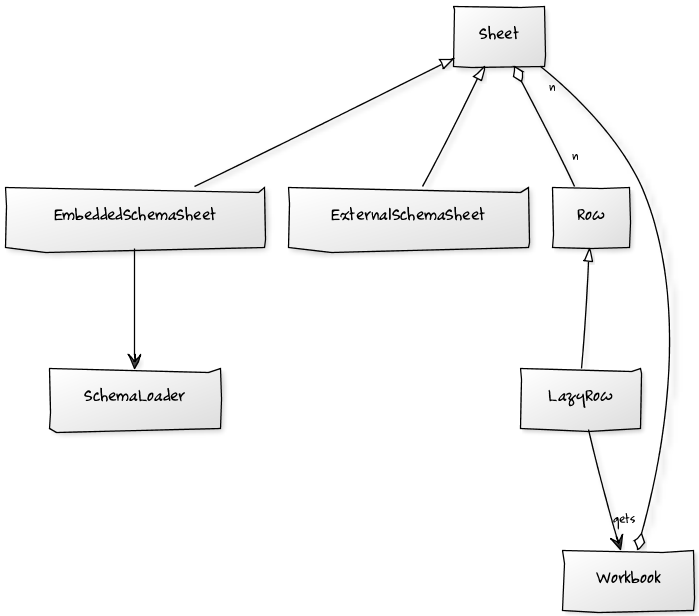
\includegraphics{sheet.png}


\subsection{Overheads}
\label{sheet:overheads}
Sheet and Row are essentially lazy sequences.

\begin{Verbatim}[commandchars=\\\{\}]
\PYG{l+s+sd}{\PYGZdq{}\PYGZdq{}\PYGZdq{}stingray.sheet \PYGZhy{}\PYGZhy{} Defines Row as  a collection of Cells and Sheet as a collection of Rows.}
\PYG{l+s+sd}{\PYGZdq{}\PYGZdq{}\PYGZdq{}}
\PYG{k+kn}{from} \PYG{n+nn}{collections} \PYG{k+kn}{import} \PYG{n}{Sequence}
\end{Verbatim}

There are two ``implicit'' dependencies, also.
A row depends on details of an {\hyperref[schema:schema.Attribute]{\code{schema.Attribute}}} and a {\hyperref[workbook/base:workbook.base.Workbook]{\code{workbook.base.Workbook}}}.
However, there's no real need to present a formal import for this.
The Attribute and Workbook are simply opaque
objects passed around as arguments.


\subsection{Sheet Class}
\label{sheet:sheet-class}\index{Sheet (class in sheet)}

\begin{fulllineitems}
\phantomsection\label{sheet:sheet.Sheet}\pysigline{\strong{class }\code{sheet.}\bfcode{Sheet}}
An iterator over the rows of data in a workbook.
Subclasses implement different bindings for the sheet's schema information.

This is largely abstract, since there's no schema binding available.
There are subclasses which have a schema binding.
See {\hyperref[sheet:sheet.ExternalSchemaSheet]{\code{sheet.ExternalSchemaSheet}}} and {\hyperref[sheet:sheet.EmbeddedSchemaSheet]{\code{sheet.EmbeddedSchemaSheet}}}.
\index{workbook (sheet.Sheet attribute)}

\begin{fulllineitems}
\phantomsection\label{sheet:sheet.Sheet.workbook}\pysigline{\bfcode{workbook}}
The \code{Workbook} which contains this Sheet.

\end{fulllineitems}

\index{name (sheet.Sheet attribute)}

\begin{fulllineitems}
\phantomsection\label{sheet:sheet.Sheet.name}\pysigline{\bfcode{name}}
The name of this sheet.

\end{fulllineitems}


\end{fulllineitems}


\begin{Verbatim}[commandchars=\\\{\}]
\PYG{k}{class} \PYG{n+nc}{Sheet}\PYG{p}{:}
    \PYG{l+s+sd}{\PYGZdq{}\PYGZdq{}\PYGZdq{}An iterator over rows.}
\PYG{l+s+sd}{        A binding to a workbook.}
\PYG{l+s+sd}{        A subclass of Sheet will be bound to a schema.}
\PYG{l+s+sd}{    \PYGZdq{}\PYGZdq{}\PYGZdq{}}
    \PYG{k}{def} \PYG{n+nf}{\PYGZus{}\PYGZus{}init\PYGZus{}\PYGZus{}}\PYG{p}{(} \PYG{n+nb+bp}{self}\PYG{p}{,} \PYG{n}{workbook}\PYG{p}{,} \PYG{n}{sheet\PYGZus{}name} \PYG{p}{)}\PYG{p}{:}
        \PYG{n+nb+bp}{self}\PYG{o}{.}\PYG{n}{workbook}\PYG{p}{,} \PYG{n+nb+bp}{self}\PYG{o}{.}\PYG{n}{name}\PYG{o}{=} \PYG{n}{workbook}\PYG{p}{,} \PYG{n}{sheet\PYGZus{}name}
    \PYG{k}{def} \PYG{n+nf}{\PYGZus{}\PYGZus{}repr\PYGZus{}\PYGZus{}}\PYG{p}{(} \PYG{n+nb+bp}{self} \PYG{p}{)}\PYG{p}{:}
        \PYG{k}{return} \PYG{l+s}{\PYGZdq{}}\PYG{l+s}{\PYGZob{}0\PYGZcb{}(\PYGZob{}1!r\PYGZcb{},\PYGZob{}2!r\PYGZcb{})}\PYG{l+s}{\PYGZdq{}}\PYG{o}{.}\PYG{n}{format}\PYG{p}{(} \PYG{n+nb+bp}{self}\PYG{o}{.}\PYG{n}{\PYGZus{}\PYGZus{}class\PYGZus{}\PYGZus{}}\PYG{o}{.}\PYG{n}{\PYGZus{}\PYGZus{}qualname\PYGZus{}\PYGZus{}}\PYG{p}{,}
            \PYG{n+nb+bp}{self}\PYG{o}{.}\PYG{n}{workbook}\PYG{p}{,} \PYG{n+nb+bp}{self}\PYG{o}{.}\PYG{n}{name} \PYG{p}{)}
    \PYG{k}{def} \PYG{n+nf}{rows}\PYG{p}{(} \PYG{n+nb+bp}{self} \PYG{p}{)}\PYG{p}{:}
        \PYG{l+s+sd}{\PYGZdq{}\PYGZdq{}\PYGZdq{}Iterate through the rows of this sheet.}
\PYG{l+s+sd}{        This is a convenient interface for {}`{}`self.workbook.rows\PYGZus{}of(self){}`{}`}
\PYG{l+s+sd}{        \PYGZdq{}\PYGZdq{}\PYGZdq{}}
        \PYG{k}{return} \PYG{n+nb+bp}{self}\PYG{o}{.}\PYG{n}{workbook}\PYG{o}{.}\PYG{n}{rows\PYGZus{}of}\PYG{p}{(} \PYG{n+nb+bp}{self} \PYG{p}{)}
\end{Verbatim}


\subsection{Row Class}
\label{sheet:row-class}\index{Row (class in sheet)}

\begin{fulllineitems}
\phantomsection\label{sheet:sheet.Row}\pysigline{\strong{class }\code{sheet.}\bfcode{Row}}
A single row in Sheet; a sequence of {\hyperref[cell:cell.Cell]{\code{cell.Cell}}} instances.

A Sheet produces this simple row-as-list.  A Schema can transform this
into row-as-dict or some even more elaborate structure.

A row depends on details of an {\hyperref[schema:schema.Attribute]{\code{schema.Attribute}}}
and a {\hyperref[workbook/base:workbook.base.Workbook]{\code{workbook.base.Workbook}}}.
This feels circular. But this Sheet/Row schema definition is really
just a convenient wrapper around the Workbook details.

The {\hyperref[cell:cell.Cell]{\code{cell.Cell}}} conversions are handled by the {\hyperref[workbook/base:workbook.base.Workbook]{\code{workbook.base.Workbook}}}.
Some Workbooks have cell content identified by position.
Some Workbooks have cell content identified by size, offset and encoding.
Therefore, we must provide the Attribute details to the Workbook
to get the Cell's value.
\index{sheet (sheet.Row attribute)}

\begin{fulllineitems}
\phantomsection\label{sheet:sheet.Row.sheet}\pysigline{\bfcode{sheet}}
The {\hyperref[sheet:sheet.Sheet]{\code{Sheet}}} which contains this row.

\end{fulllineitems}

\index{data (sheet.Row attribute)}

\begin{fulllineitems}
\phantomsection\label{sheet:sheet.Row.data}\pysigline{\bfcode{data}}
The sequence of \code{Cell} values for this row.

\end{fulllineitems}


\end{fulllineitems}


\begin{Verbatim}[commandchars=\\\{\}]
\PYG{k}{class} \PYG{n+nc}{Row}\PYG{p}{(} \PYG{n}{Sequence} \PYG{p}{)}\PYG{p}{:}
    \PYG{l+s+sd}{\PYGZdq{}\PYGZdq{}\PYGZdq{}Eager Row: a tuple of Cell values.\PYGZdq{}\PYGZdq{}\PYGZdq{}}
    \PYG{k}{def} \PYG{n+nf}{\PYGZus{}\PYGZus{}init\PYGZus{}\PYGZus{}}\PYG{p}{(} \PYG{n+nb+bp}{self}\PYG{p}{,} \PYG{n}{sheet}\PYG{p}{,} \PYG{o}{*}\PYG{n}{data} \PYG{p}{)}\PYG{p}{:}
        \PYG{l+s+sd}{\PYGZdq{}\PYGZdq{}\PYGZdq{}Build another Row.}

\PYG{l+s+sd}{        :param sheet: the containing sheet.}
\PYG{l+s+sd}{        :param *data: the various Cell values in this row}
\PYG{l+s+sd}{        \PYGZdq{}\PYGZdq{}\PYGZdq{}}
        \PYG{n+nb+bp}{self}\PYG{o}{.}\PYG{n}{sheet}\PYG{o}{=} \PYG{n}{sheet}
        \PYG{n+nb+bp}{self}\PYG{o}{.}\PYG{n}{data}\PYG{o}{=} \PYG{n}{data}
    \PYG{k}{def} \PYG{n+nf}{cell}\PYG{p}{(} \PYG{n+nb+bp}{self}\PYG{p}{,} \PYG{n}{attribute} \PYG{p}{)}\PYG{p}{:}
        \PYG{l+s+sd}{\PYGZdq{}\PYGZdq{}\PYGZdq{}Get a specific cell, based on a schema Attribute.}

\PYG{l+s+sd}{        :param attribute: The attribute\PYGZsq{}s value to return.}
\PYG{l+s+sd}{        \PYGZdq{}\PYGZdq{}\PYGZdq{}}
        \PYG{k}{return} \PYG{n+nb+bp}{self}\PYG{o}{.}\PYG{n}{sheet}\PYG{o}{.}\PYG{n}{workbook}\PYG{o}{.}\PYG{n}{row\PYGZus{}get}\PYG{p}{(} \PYG{n+nb+bp}{self}\PYG{p}{,} \PYG{n}{attribute} \PYG{p}{)}
\end{Verbatim}

Basic Sequence features

\begin{Verbatim}[commandchars=\\\{\}]
\PYG{k}{def} \PYG{n+nf}{\PYGZus{}\PYGZus{}len\PYGZus{}\PYGZus{}}\PYG{p}{(} \PYG{n+nb+bp}{self} \PYG{p}{)}\PYG{p}{:}
    \PYG{k}{return} \PYG{n+nb}{len}\PYG{p}{(}\PYG{n+nb+bp}{self}\PYG{o}{.}\PYG{n}{data}\PYG{p}{)}
\PYG{k}{def} \PYG{n+nf}{\PYGZus{}\PYGZus{}iter\PYGZus{}\PYGZus{}}\PYG{p}{(} \PYG{n+nb+bp}{self} \PYG{p}{)}\PYG{p}{:}
    \PYG{k}{return} \PYG{n+nb}{iter}\PYG{p}{(}\PYG{n+nb+bp}{self}\PYG{o}{.}\PYG{n}{data}\PYG{p}{)}
\PYG{k}{def} \PYG{n+nf}{\PYGZus{}\PYGZus{}contains\PYGZus{}\PYGZus{}}\PYG{p}{(} \PYG{n+nb+bp}{self}\PYG{p}{,} \PYG{n}{cell} \PYG{p}{)}\PYG{p}{:}
    \PYG{k}{return} \PYG{n+nb}{any}\PYG{p}{(} \PYG{n}{cell}\PYG{o}{.}\PYG{n}{value} \PYG{o}{==} \PYG{n}{d}\PYG{o}{.}\PYG{n}{value} \PYG{k}{for} \PYG{n}{d} \PYG{o+ow}{in} \PYG{n+nb+bp}{self}\PYG{o}{.}\PYG{n}{data} \PYG{p}{)}
\PYG{k}{def} \PYG{n+nf}{\PYGZus{}\PYGZus{}getitem\PYGZus{}\PYGZus{}}\PYG{p}{(} \PYG{n+nb+bp}{self}\PYG{p}{,} \PYG{n}{index} \PYG{p}{)}\PYG{p}{:}
    \PYG{k}{return} \PYG{n+nb+bp}{self}\PYG{o}{.}\PYG{n}{data}\PYG{p}{[}\PYG{n}{index}\PYG{p}{]}
\end{Verbatim}

To approach the \code{csv.DictReader} API (without the eager processing),
we need make the \code{Row} API slightly more fluent with a \code{by\_name()}
method.

\begin{Verbatim}[commandchars=\\\{\}]
\PYG{k}{def} \PYG{n+nf}{by\PYGZus{}name}\PYG{p}{(} \PYG{n+nb+bp}{self}\PYG{p}{,} \PYG{n}{name} \PYG{p}{)}\PYG{p}{:}
    \PYG{n}{attr}\PYG{o}{=} \PYG{n+nb+bp}{self}\PYG{o}{.}\PYG{n}{sheet}\PYG{o}{.}\PYG{n}{schema}\PYG{o}{.}\PYG{n}{get\PYGZus{}name}\PYG{p}{(}\PYG{n}{name}\PYG{p}{)}
    \PYG{k}{return} \PYG{n+nb+bp}{self}\PYG{o}{.}\PYG{n}{cell}\PYG{p}{(} \PYG{n}{attr} \PYG{p}{)}
\end{Verbatim}

Note that the presumption in this interface is that the Attribute is
sufficiently detailed to specify a single {\hyperref[cell:cell.Cell]{\code{cell.Cell}}}.
For non-COBOL workbooks, this is perfectly true.

For COBOL, however, there are groups and occurs clauses, meaning that a single Attribute can
represent multiple {\hyperref[cell:cell.Cell]{\code{cell.Cell}}} instances.
Which one do we mean?  And how do we specify this selection?
\begin{itemize}
\item {} 
The \code{sheet.Row.cell()} method can return a structure with all the values.
Ordinary Python can then pick apart the instances.
This requires working up the DDE hierarchy to locate all of the applicable
``occurs'' by to construct the proper dimensionality of an attribute.

It also means getting all of the values to create a tuple or nested
tuple-of-tuple structure for the various dimensions. Eager processing isn't
going to work out well.

\item {} 
The \code{schema.Attribute.index} method
selects data from the row in the workbook.  This applies the indices
to the Attribute to compute the required offset into the source data.

We're constrained by the laziness requirement of COBOL to lean toward the
this implementation.

\end{itemize}
\index{LazyRow (class in sheet)}

\begin{fulllineitems}
\phantomsection\label{sheet:sheet.LazyRow}\pysigline{\strong{class }\code{sheet.}\bfcode{LazyRow}}
When we can't eagerly build all {\hyperref[cell:cell.Cell]{\code{cell.Cell}}} instances for a given
row, this class provides the proper API.

A COBOL REDEFINES clause may make the bytes invalid in all but one of the
aliases for an attribute.  Also, there's no formal \code{NULL} value in COBOL, so
optional fields can have invalid data.

Further, we may have Occurs Depending On. This means we can't set size and
offset until we can access actual data.

For these reasons, we have a {\hyperref[sheet:sheet.LazyRow]{\code{sheet.LazyRow}}}, which conforms to the
interface for a {\hyperref[sheet:sheet.Row]{\code{Row}}}, but isn't an actual sequence. No data is
processed until the \code{LazyRow.\_\_getitem\_\_()} method is used.
\index{sheet (sheet.LazyRow attribute)}

\begin{fulllineitems}
\phantomsection\label{sheet:sheet.LazyRow.sheet}\pysigline{\bfcode{sheet}}
The {\hyperref[sheet:sheet.Sheet]{\code{Sheet}}} to which this row belongs.

\end{fulllineitems}

\index{\_state (sheet.LazyRow attribute)}

\begin{fulllineitems}
\phantomsection\label{sheet:sheet.LazyRow._state}\pysigline{\bfcode{\_state}}
The worksheet's internal state information, required
to perform lazy extraction of the cell values. The LazyRow
superclass doesn't use this. A subclass may need it.

\end{fulllineitems}


\end{fulllineitems}


\begin{Verbatim}[commandchars=\\\{\}]
\PYG{k}{class} \PYG{n+nc}{LazyRow}\PYG{p}{(} \PYG{n}{Sequence} \PYG{p}{)}\PYG{p}{:}
    \PYG{l+s+sd}{\PYGZdq{}\PYGZdq{}\PYGZdq{}Lazy Row: a tuple\PYGZhy{}like sequence of Cell values.\PYGZdq{}\PYGZdq{}\PYGZdq{}}
    \PYG{k}{def} \PYG{n+nf}{\PYGZus{}\PYGZus{}init\PYGZus{}\PYGZus{}}\PYG{p}{(} \PYG{n+nb+bp}{self}\PYG{p}{,} \PYG{n}{sheet}\PYG{p}{,} \PYG{o}{*}\PYG{o}{*}\PYG{n}{state} \PYG{p}{)}\PYG{p}{:}
        \PYG{l+s+sd}{\PYGZdq{}\PYGZdq{}\PYGZdq{}Build another Row.}

\PYG{l+s+sd}{        :param sheet: the containing sheet.}
\PYG{l+s+sd}{        :param **state: worksheet\PYGZhy{}specific state value to save.}
\PYG{l+s+sd}{        \PYGZdq{}\PYGZdq{}\PYGZdq{}}
        \PYG{n+nb+bp}{self}\PYG{o}{.}\PYG{n}{sheet}\PYG{o}{=} \PYG{n}{sheet}
        \PYG{n+nb+bp}{self}\PYG{o}{.}\PYG{n}{\PYGZus{}state}\PYG{o}{=} \PYG{n}{state}
        \PYG{n+nb}{super}\PYG{p}{(}\PYG{p}{)}\PYG{o}{.}\PYG{n}{\PYGZus{}\PYGZus{}init\PYGZus{}\PYGZus{}}\PYG{p}{(}\PYG{p}{)}
    \PYG{k}{def} \PYG{n+nf}{\PYGZus{}\PYGZus{}repr\PYGZus{}\PYGZus{}}\PYG{p}{(} \PYG{n+nb+bp}{self} \PYG{p}{)}\PYG{p}{:}
        \PYG{k}{return} \PYG{l+s}{\PYGZdq{}}\PYG{l+s}{LazyRow(sheet=\PYGZob{}0!r\PYGZcb{}, state=\PYGZob{}1!r\PYGZcb{})}\PYG{l+s}{\PYGZdq{}}\PYG{o}{.}\PYG{n}{format}\PYG{p}{(} \PYG{n+nb+bp}{self}\PYG{o}{.}\PYG{n}{sheet}\PYG{p}{,} \PYG{n+nb+bp}{self}\PYG{o}{.}\PYG{n}{\PYGZus{}state} \PYG{p}{)}
    \PYG{k}{def} \PYG{n+nf}{cell}\PYG{p}{(} \PYG{n+nb+bp}{self}\PYG{p}{,} \PYG{n}{attribute} \PYG{p}{)}\PYG{p}{:}
        \PYG{l+s+sd}{\PYGZdq{}\PYGZdq{}\PYGZdq{}Get a specific cell, based on a schema Attribute.}

\PYG{l+s+sd}{        :param attribute: The attribute\PYGZsq{}s value to return.}
\PYG{l+s+sd}{        \PYGZdq{}\PYGZdq{}\PYGZdq{}}
        \PYG{k}{return} \PYG{n+nb+bp}{self}\PYG{o}{.}\PYG{n}{sheet}\PYG{o}{.}\PYG{n}{workbook}\PYG{o}{.}\PYG{n}{row\PYGZus{}get}\PYG{p}{(} \PYG{n+nb+bp}{self}\PYG{p}{,} \PYG{n}{attribute} \PYG{p}{)}
\end{Verbatim}

Basic Sequence features

\begin{Verbatim}[commandchars=\\\{\}]
\PYG{k}{def} \PYG{n+nf}{\PYGZus{}\PYGZus{}len\PYGZus{}\PYGZus{}}\PYG{p}{(} \PYG{n+nb+bp}{self} \PYG{p}{)}\PYG{p}{:}
    \PYG{k}{return} \PYG{n+nb}{len}\PYG{p}{(}\PYG{n+nb+bp}{self}\PYG{o}{.}\PYG{n}{sheet}\PYG{o}{.}\PYG{n}{schema}\PYG{p}{)}
\PYG{k}{def} \PYG{n+nf}{\PYGZus{}\PYGZus{}iter\PYGZus{}\PYGZus{}}\PYG{p}{(} \PYG{n+nb+bp}{self} \PYG{p}{)}\PYG{p}{:}
    \PYG{k}{for} \PYG{n}{attribute} \PYG{o+ow}{in} \PYG{n+nb+bp}{self}\PYG{o}{.}\PYG{n}{sheet}\PYG{o}{.}\PYG{n}{schema}\PYG{p}{:}
        \PYG{k}{try}\PYG{p}{:}
            \PYG{k}{yield} \PYG{n+nb+bp}{self}\PYG{o}{.}\PYG{n}{sheet}\PYG{o}{.}\PYG{n}{workbook}\PYG{o}{.}\PYG{n}{row\PYGZus{}get}\PYG{p}{(} \PYG{n+nb+bp}{self}\PYG{p}{,} \PYG{n}{attribute} \PYG{p}{)}
        \PYG{k}{except} \PYG{n+ne}{Exception} \PYG{k}{as} \PYG{n}{e}\PYG{p}{:}
            \PYG{k}{yield} \PYG{n+nb+bp}{None}
\PYG{k}{def} \PYG{n+nf}{\PYGZus{}\PYGZus{}contains\PYGZus{}\PYGZus{}}\PYG{p}{(} \PYG{n+nb+bp}{self}\PYG{p}{,} \PYG{n}{cell} \PYG{p}{)}\PYG{p}{:}
    \PYG{k}{for} \PYG{n}{attribute} \PYG{o+ow}{in} \PYG{n+nb+bp}{self}\PYG{o}{.}\PYG{n}{sheet}\PYG{o}{.}\PYG{n}{schema}\PYG{p}{:}
        \PYG{k}{try}\PYG{p}{:}
            \PYG{n}{col}\PYG{o}{=} \PYG{n+nb+bp}{self}\PYG{o}{.}\PYG{n}{sheet}\PYG{o}{.}\PYG{n}{workbook}\PYG{o}{.}\PYG{n}{row\PYGZus{}get}\PYG{p}{(} \PYG{n+nb+bp}{self}\PYG{p}{,} \PYG{n}{attribute} \PYG{p}{)}
        \PYG{k}{except} \PYG{n+ne}{Exception} \PYG{k}{as} \PYG{n}{e}\PYG{p}{:}
            \PYG{k}{pass}
        \PYG{k}{if} \PYG{n}{col}\PYG{o}{.}\PYG{n}{value} \PYG{o}{==} \PYG{n}{cell}\PYG{o}{.}\PYG{n}{value}\PYG{p}{:}
            \PYG{k}{return} \PYG{n+nb+bp}{True}
\PYG{k}{def} \PYG{n+nf}{\PYGZus{}\PYGZus{}getitem\PYGZus{}\PYGZus{}}\PYG{p}{(} \PYG{n+nb+bp}{self}\PYG{p}{,} \PYG{n}{index} \PYG{p}{)}\PYG{p}{:}
    \PYG{n}{attribute}\PYG{o}{=} \PYG{n+nb+bp}{self}\PYG{o}{.}\PYG{n}{sheet}\PYG{o}{.}\PYG{n}{schema}\PYG{p}{[}\PYG{n}{index}\PYG{p}{]}
    \PYG{k}{return} \PYG{n+nb+bp}{self}\PYG{o}{.}\PYG{n}{sheet}\PYG{o}{.}\PYG{n}{workbook}\PYG{o}{.}\PYG{n}{row\PYGZus{}get}\PYG{p}{(} \PYG{n+nb+bp}{self}\PYG{p}{,} \PYG{n}{attribute} \PYG{p}{)}
\end{Verbatim}

To approach the \code{csv.DictReader} API (without the eager processing),
we could make the \code{Row} API slightly more fluent with a \code{by\_name()}
method.

\begin{Verbatim}[commandchars=\\\{\}]
\PYG{k}{def} \PYG{n+nf}{by\PYGZus{}name}\PYG{p}{(} \PYG{n+nb+bp}{self}\PYG{p}{,} \PYG{n}{name} \PYG{p}{)}\PYG{p}{:}
    \PYG{n}{attr}\PYG{o}{=} \PYG{n+nb+bp}{self}\PYG{o}{.}\PYG{n}{sheet}\PYG{o}{.}\PYG{n}{schema}\PYG{o}{.}\PYG{n}{get\PYGZus{}name}\PYG{p}{(}\PYG{n}{name}\PYG{p}{)}
    \PYG{k}{return} \PYG{n+nb+bp}{self}\PYG{o}{.}\PYG{n}{cell}\PYG{p}{(}\PYG{n}{attr}\PYG{p}{)}
\end{Verbatim}

This isn't implemented, because it doesn't seem very helpful.


\subsection{ExternalSchemaSheet Class}
\label{sheet:externalschemasheet-class}\index{ExternalSchemaSheet (class in sheet)}

\begin{fulllineitems}
\phantomsection\label{sheet:sheet.ExternalSchemaSheet}\pysigline{\strong{class }\code{sheet.}\bfcode{ExternalSchemaSheet}}
A Sheet bound to a schema can be used to fetch data. This is a
concrete subclass of {\hyperref[sheet:sheet.Sheet]{\code{Sheet}}}.

A Sheet with an external schema can have one of two sources for
the bound schema.
\begin{itemize}
\item {} 
An external sheet that doesn't have row headers to embed the schema information.
In this case, an eager Workbook Row can eagerly create a Sequence of {\hyperref[cell:cell.Cell]{\code{cell.Cell}}} instances.
The Schema information can be associated by position.

\item {} 
A Sheet that is really a COBOL or Fixed format file.
In this case, the Workbook cannot create a sequence of {\hyperref[cell:cell.Cell]{\code{cell.Cell}}} instances.
Instead, the Sheet (which has schema information) must
provide a LazyRow with deferred Cell conversions.

\end{itemize}

\end{fulllineitems}


\begin{Verbatim}[commandchars=\\\{\}]
\PYG{k}{class} \PYG{n+nc}{ExternalSchemaSheet}\PYG{p}{(} \PYG{n}{Sheet} \PYG{p}{)}\PYG{p}{:}
    \PYG{l+s+sd}{\PYGZdq{}\PYGZdq{}\PYGZdq{}A Sheet with an external Schema.\PYGZdq{}\PYGZdq{}\PYGZdq{}}
    \PYG{k}{def} \PYG{n+nf}{\PYGZus{}\PYGZus{}init\PYGZus{}\PYGZus{}}\PYG{p}{(} \PYG{n+nb+bp}{self}\PYG{p}{,} \PYG{n}{workbook}\PYG{p}{,} \PYG{n}{sheet\PYGZus{}name}\PYG{p}{,} \PYG{n}{schema} \PYG{p}{)}\PYG{p}{:}
        \PYG{l+s+sd}{\PYGZdq{}\PYGZdq{}\PYGZdq{}Initialize a sheet for processing.}

\PYG{l+s+sd}{        :param workbook: the containing workbook}
\PYG{l+s+sd}{        :param sheet\PYGZus{}name: the specific sheet to locate within the Workbook}
\PYG{l+s+sd}{        :param schema: the :py:class:{}`schema.Schema{}` schema definition.}
\PYG{l+s+sd}{        \PYGZdq{}\PYGZdq{}\PYGZdq{}}
        \PYG{n+nb}{super}\PYG{p}{(}\PYG{p}{)}\PYG{o}{.}\PYG{n}{\PYGZus{}\PYGZus{}init\PYGZus{}\PYGZus{}}\PYG{p}{(} \PYG{n}{workbook}\PYG{p}{,} \PYG{n}{sheet\PYGZus{}name} \PYG{p}{)}
        \PYG{n+nb+bp}{self}\PYG{o}{.}\PYG{n}{schema}\PYG{o}{=} \PYG{n}{schema}
    \PYG{k}{def} \PYG{n+nf}{rows}\PYG{p}{(} \PYG{n+nb+bp}{self} \PYG{p}{)}\PYG{p}{:}
        \PYG{l+s+sd}{\PYGZdq{}\PYGZdq{}\PYGZdq{}Iterate through the rows of this sheet.\PYGZdq{}\PYGZdq{}\PYGZdq{}}
        \PYG{k}{return} \PYG{n+nb+bp}{self}\PYG{o}{.}\PYG{n}{workbook}\PYG{o}{.}\PYG{n}{rows\PYGZus{}of}\PYG{p}{(} \PYG{n+nb+bp}{self} \PYG{p}{)}
\end{Verbatim}


\subsection{EmbeddedSchemaSheet Class}
\label{sheet:embeddedschemasheet-class}\index{EmbeddedSchemaSheet (class in sheet)}

\begin{fulllineitems}
\phantomsection\label{sheet:sheet.EmbeddedSchemaSheet}\pysigline{\strong{class }\code{sheet.}\bfcode{EmbeddedSchemaSheet}}
A sheet bound to a schema can be used to fetch data. This is a
concrete subclass of {\hyperref[sheet:sheet.Sheet]{\code{Sheet}}}.

A sheet with an embedded schema must also have a {\hyperref[schema_loader:schema.loader.SchemaLoader]{\code{schema.loader.SchemaLoader}}} class provided.
The loader
is invoked to build the {\hyperref[schema:schema.Schema]{\code{schema.Schema}}} object that's bound
to the sheet.

The {\hyperref[schema_loader:schema.loader.SchemaLoader]{\code{schema.loader.SchemaLoader}}} is also used to return the rest of the rows;
those that weren't used to build the schema.
\index{loader (sheet.EmbeddedSchemaSheet attribute)}

\begin{fulllineitems}
\phantomsection\label{sheet:sheet.EmbeddedSchemaSheet.loader}\pysigline{\bfcode{loader}}
The \code{Loader} used to build schema from rows in this sheet.

\end{fulllineitems}


\end{fulllineitems}


\begin{Verbatim}[commandchars=\\\{\}]
\PYG{k}{class} \PYG{n+nc}{EmbeddedSchemaSheet}\PYG{p}{(} \PYG{n}{ExternalSchemaSheet} \PYG{p}{)}\PYG{p}{:}
    \PYG{l+s+sd}{\PYGZdq{}\PYGZdq{}\PYGZdq{}A Sheet with a Schema embedded in it.\PYGZdq{}\PYGZdq{}\PYGZdq{}}
    \PYG{k}{def} \PYG{n+nf}{\PYGZus{}\PYGZus{}init\PYGZus{}\PYGZus{}}\PYG{p}{(} \PYG{n+nb+bp}{self}\PYG{p}{,} \PYG{n}{workbook}\PYG{p}{,} \PYG{n}{sheet\PYGZus{}name}\PYG{p}{,} \PYG{n}{loader\PYGZus{}class} \PYG{p}{)}\PYG{p}{:}
        \PYG{l+s+sd}{\PYGZdq{}\PYGZdq{}\PYGZdq{}Initialize a sheet for processing.}

\PYG{l+s+sd}{        :param workbook: the containing workbook}
\PYG{l+s+sd}{        :param sheet\PYGZus{}name: the specific sheet to locate within the Workbook}
\PYG{l+s+sd}{        :param loader\PYGZus{}class: the :py:class:{}`schema.loader.SchemaLoader{}`}
\PYG{l+s+sd}{        schema loader to load the schema from the sheet.}

\PYG{l+s+sd}{        Apply the loader to the given sheet of the workbook to get schema}
\PYG{l+s+sd}{        and rows.}
\PYG{l+s+sd}{        \PYGZdq{}\PYGZdq{}\PYGZdq{}}
        \PYG{n}{s} \PYG{o}{=} \PYG{n}{Sheet}\PYG{p}{(} \PYG{n}{workbook}\PYG{p}{,} \PYG{n}{sheet\PYGZus{}name} \PYG{p}{)}
        \PYG{n+nb+bp}{self}\PYG{o}{.}\PYG{n}{loader} \PYG{o}{=} \PYG{n}{loader\PYGZus{}class}\PYG{p}{(} \PYG{n}{s} \PYG{p}{)}
        \PYG{n}{schema}\PYG{o}{=} \PYG{n+nb+bp}{self}\PYG{o}{.}\PYG{n}{loader}\PYG{o}{.}\PYG{n}{schema}\PYG{p}{(}\PYG{p}{)}
        \PYG{n+nb}{super}\PYG{p}{(}\PYG{p}{)}\PYG{o}{.}\PYG{n}{\PYGZus{}\PYGZus{}init\PYGZus{}\PYGZus{}}\PYG{p}{(} \PYG{n}{workbook}\PYG{p}{,} \PYG{n}{sheet\PYGZus{}name}\PYG{p}{,} \PYG{n}{schema}\PYG{o}{=}\PYG{n}{schema} \PYG{p}{)}
    \PYG{k}{def} \PYG{n+nf}{rows}\PYG{p}{(} \PYG{n+nb+bp}{self} \PYG{p}{)}\PYG{p}{:}
        \PYG{l+s+sd}{\PYGZdq{}\PYGZdq{}\PYGZdq{}The parser will skip over the headers.\PYGZdq{}\PYGZdq{}\PYGZdq{}}
        \PYG{k}{return} \PYG{n+nb+bp}{self}\PYG{o}{.}\PYG{n}{loader}\PYG{o}{.}\PYG{n}{rows}\PYG{p}{(}\PYG{p}{)}
\end{Verbatim}

Since the rows are already properly encoded as {\hyperref[cell:cell.Cell]{\code{cell.Cell}}} instances,
no further processing is required by the Sheet or the Loader.


\subsection{Rows of a Sheet}
\label{sheet:rows-of-a-sheet}
Note that the \code{csv} design pattern for each row involves two subclasses
with the same method names but different results.  One
returns a \code{dict} of cells, keyed by field names, the other returns a \code{list} of cells,
indexed by position.

The dict-based processing has the advantage of clarity: cells are named row{[}'cell'{]}.
It has the disadvantage of not coping well with duplicate column names or data
which breaks first normal form.

We can't follow the \code{csv} design pattern.  Instead we do the following.
\begin{itemize}
\item {} 
A {\hyperref[sheet:sheet.Row]{\code{sheet.Row}}} is a sequence of {\hyperref[cell:cell.Cell]{\code{cell.Cell}}} instances.
It may be lazy or it may be eager.

\item {} 
To use names, a {\hyperref[schema:schema.Schema]{\code{schema.Schema}}} must be used to fetch {\hyperref[cell:cell.Cell]{\code{cell.Cell}}}
instances from the {\hyperref[sheet:sheet.Row]{\code{sheet.Row}}} object. The schema translates names to positions.

\item {} 
To create dict-like access to {\hyperref[cell:cell.Cell]{\code{cell.Cell}}}  instances,
the {\hyperref[schema:schema.Schema]{\code{schema.Schema}}} can be turned into a dictionary.  The row itself
is not a dictionary, just the schema. The row is still a Sequence.

This ``schema-as-dict'' can still be used with a properly
lazy {\hyperref[sheet:sheet.Row]{\code{sheet.Row}}} to create {\hyperref[cell:cell.Cell]{\code{cell.Cell}}} instances.

\end{itemize}

We need the lazy evaluation of a row that fetches data based on {\hyperref[schema:schema.Attribute]{\code{schema.Attribute}}}
details in order to cope with COBOL \code{REDEFINES}.  It also allows us to cope
with the unfortunately common problem of duplicate column names in conventional
spreadsheets.

We can have application programming which looks like this to process a
Row as sequence:

\begin{Verbatim}[commandchars=\\\{\}]
\PYG{k}{for} \PYG{n}{row} \PYG{o+ow}{in} \PYG{n}{sheet}\PYG{o}{.}\PYG{n}{rows}\PYG{p}{(}\PYG{p}{)}\PYG{p}{:}
    \PYG{n}{row}\PYG{p}{[}\PYG{n}{i}\PYG{p}{]} \PYG{c}{\PYGZsh{} instance of Cell}
    \PYG{n}{sheet}\PYG{o}{.}\PYG{n}{schema}\PYG{p}{[}\PYG{n}{i}\PYG{p}{]}\PYG{o}{.}\PYG{n}{name} \PYG{c}{\PYGZsh{} name attribute of Schema Attribute}
\end{Verbatim}

Row as dict is a common alternative.  If we have unique column names in the schema,
We can than use application programming that looks like this.

\begin{Verbatim}[commandchars=\\\{\}]
\PYG{n}{schema\PYGZus{}dict} \PYG{o}{=} \PYG{n+nb}{dict}\PYG{p}{(}\PYG{p}{(}\PYG{n}{a}\PYG{o}{.}\PYG{n}{name}\PYG{p}{,} \PYG{n}{a}\PYG{p}{)} \PYG{k}{for} \PYG{n}{a} \PYG{o+ow}{in} \PYG{n}{sheet}\PYG{o}{.}\PYG{n}{schema}\PYG{p}{)}
\PYG{k}{for} \PYG{n}{row} \PYG{o+ow}{in} \PYG{n}{sheet}\PYG{o}{.}\PYG{n}{rows}\PYG{p}{(}\PYG{p}{)}\PYG{p}{:}
    \PYG{n}{row}\PYG{o}{.}\PYG{n}{cell}\PYG{p}{(}\PYG{n}{schema\PYGZus{}dict}\PYG{p}{[}\PYG{l+s}{\PYGZsq{}}\PYG{l+s}{name}\PYG{l+s}{\PYGZsq{}}\PYG{p}{]}\PYG{p}{)} \PYG{c}{\PYGZsh{} instance of Cell}
    \PYG{n}{row\PYGZus{}as\PYGZus{}dict}\PYG{o}{=} \PYG{n+nb}{dict}\PYG{p}{(}
        \PYG{p}{(}\PYG{n}{a}\PYG{o}{.}\PYG{n}{name}\PYG{p}{,} \PYG{n}{row}\PYG{o}{.}\PYG{n}{cell}\PYG{p}{(}\PYG{n}{a}\PYG{p}{)}\PYG{p}{)} \PYG{k}{for} \PYG{n}{a} \PYG{o+ow}{in} \PYG{n}{sheet}\PYG{o}{.}\PYG{n}{schema}\PYG{p}{)}
    \PYG{n}{row\PYGZus{}as\PYGZus{}dict}\PYG{p}{[}\PYG{l+s}{\PYGZsq{}}\PYG{l+s}{name}\PYG{l+s}{\PYGZsq{}}\PYG{p}{]} \PYG{c}{\PYGZsh{} instance of Cell}
\end{Verbatim}

This handles the COBOL case, where rows must be lazy.
This includes the \code{REDEFINES} and occurs clauses.
This assures proper packed decimal conversion of redefined fields.


\section{Schema Package -- Schema and Attribute Definitions}
\label{schema:module-schema}\label{schema:schema}\label{schema::doc}\label{schema:schema-package-schema-and-attribute-definitions}\index{schema (module)}
A \emph{Schema} contains data descriptions.  It's a collection of \emph{Attribute} specifications.

For our purposes, we're trying to cover the following bases:
\begin{itemize}
\item {} 
Workbooks in a variety of forms: CSV, Tab, XLSX, ODS, etc.
The common feature of these schema is that they're flat.  A single
index (or name) identifies each column.

The schema can be in a variety of places.
\begin{itemize}
\item {} 
The schema may be a header row within a sheet.

\item {} 
The schema may be elsewhere in the sheet.  It may be a header
that's not the first row.

\item {} 
The schema may be in a separate document.

\end{itemize}

\item {} 
COBOL Files. The schema is highly structured: a path must be
used to unambiguously identify each field. Some COBOL schema are
designed so that all leaf names are unique.

The schema is a separate document, encoded in
COBOL source code.

\end{itemize}

We'll also happen to cover relational database table definitions.  However,
this isn't our focus.  This is simply coincidence.

Note that we are not trying to cover XML schemas or a \textbf{complete} relational
database schema. There are a lot of possible features not present here.


\subsection{Load a Schema Use Case}
\label{schema:load-a-schema-use-case}
The objective of this module is to provide a handy base class family
that can be used to load schema information from any of a variety
of sources.
\begin{itemize}
\item {} 
Embedded schema in a sheet of a workbook.  Either a header row
or some more complex parsing.  This implies some kind of schema
parser that reads a workbook sheet and gets little more than
column names and ordinal positions.

\item {} 
External schema in another workbook.  This implies a
parser that gathers some information (name, type, position, offset,
or size) from a sheet using a fixed schema.

\item {} 
External schema in COBOL.  This implies a parser for COBOL source.

\end{itemize}

Embedded schema loading would look like this.
\begin{alltt}
with \emph{open} as wb:
    counts= defauldict( int )
    sheet = EmbeddedSchemaSheet( workbook, `Sheet1', HeadingRowSchemaLoader )
    counts= process\_sheet( sheet )
    pprint.pprint( counts )
\end{alltt}

The schema object isn't made explicit.  It's available in \code{sheet.schema}.

External schema loading would look like this.
\begin{alltt}
with \emph{open schema} as wb\_s:
    esl = ExternalSchemaLoader( wb\_s, `Schema' )
    schema = esl.load()
with \emph{open data} as wb:
    sheet = ExternalSchemaSheet( wb, `Sheet1', schema )
    counts= process\_sheet( sheet )
    pprint.pprint( counts )
\end{alltt}


\subsection{Use a Schema Use Case}
\label{schema:use-a-schema-use-case}
We use a schema to access fields by name. Here's the use case from {\hyperref[introduction:intro]{\emph{Introduction}}}.

\begin{Verbatim}[commandchars=\\\{\}]
\PYG{n}{foo}\PYG{o}{=} \PYG{n}{row}\PYG{p}{[}\PYG{l+s}{\PYGZsq{}}\PYG{l+s}{foo}\PYG{l+s}{\PYGZsq{}}\PYG{p}{]}\PYG{o}{.}\PYG{n}{to\PYGZus{}str}\PYG{p}{(}\PYG{p}{)}

\PYG{n}{bar}\PYG{o}{=} \PYG{n}{row}\PYG{p}{[}\PYG{l+s}{\PYGZsq{}}\PYG{l+s}{bar}\PYG{l+s}{\PYGZsq{}}\PYG{p}{]}\PYG{o}{.}\PYG{n}{to\PYGZus{}float}\PYG{p}{(}\PYG{p}{)}
\end{Verbatim}

This, of course, only works in the cases where the field name
is unique and the row's values can be built eagerly.  The good news
is that 80\% of the time this is true.  The other 20\% of the time, we
need something more complex.

For the 80\% case, we can do this.

\begin{Verbatim}[commandchars=\\\{\}]
\PYG{k}{for} \PYG{n}{row\PYGZus{}seq} \PYG{o+ow}{in} \PYG{n}{sheet}\PYG{o}{.}\PYG{n}{rows}\PYG{p}{(}\PYG{p}{)}\PYG{p}{:}
    \PYG{n}{row}\PYG{o}{=} \PYG{n+nb}{dict}\PYG{p}{(}
        \PYG{p}{(}\PYG{n}{a}\PYG{o}{.}\PYG{n}{name}\PYG{p}{,} \PYG{n}{row\PYGZus{}seq}\PYG{o}{.}\PYG{n}{cell}\PYG{p}{(}\PYG{n}{a}\PYG{p}{)}\PYG{p}{)}
        \PYG{k}{for} \PYG{n}{a} \PYG{o+ow}{in} \PYG{n}{schema}
    \PYG{p}{)}
    \PYG{n}{foo}\PYG{o}{=} \PYG{n}{row}\PYG{p}{[}\PYG{l+s}{\PYGZsq{}}\PYG{l+s}{foo}\PYG{l+s}{\PYGZsq{}}\PYG{p}{]}\PYG{o}{.}\PYG{n}{to\PYGZus{}str}\PYG{p}{(}\PYG{p}{)}
    \PYG{n}{bar}\PYG{o}{=} \PYG{n}{row}\PYG{p}{[}\PYG{l+s}{\PYGZsq{}}\PYG{l+s}{bar}\PYG{l+s}{\PYGZsq{}}\PYG{p}{]}\PYG{o}{.}\PYG{n}{to\PYGZus{}float}\PYG{p}{(}\PYG{p}{)}
\end{Verbatim}

Or this.

\begin{Verbatim}[commandchars=\\\{\}]
\PYG{k}{for} \PYG{n}{row} \PYG{o+ow}{in} \PYG{n}{schema}\PYG{o}{.}\PYG{n}{rows\PYGZus{}as\PYGZus{}dict\PYGZus{}iter}\PYG{p}{(} \PYG{n}{sheet}\PYG{o}{.}\PYG{n}{rows}\PYG{p}{(}\PYG{p}{)} \PYG{p}{)}\PYG{p}{:}
    \PYG{n}{foo}\PYG{o}{=} \PYG{n}{row}\PYG{p}{[}\PYG{l+s}{\PYGZsq{}}\PYG{l+s}{foo}\PYG{l+s}{\PYGZsq{}}\PYG{p}{]}\PYG{o}{.}\PYG{n}{to\PYGZus{}str}\PYG{p}{(}\PYG{p}{)}
    \PYG{n}{bar}\PYG{o}{=} \PYG{n}{row}\PYG{p}{[}\PYG{l+s}{\PYGZsq{}}\PYG{l+s}{bar}\PYG{l+s}{\PYGZsq{}}\PYG{p}{]}\PYG{o}{.}\PYG{n}{to\PYGZus{}float}\PYG{p}{(}\PYG{p}{)}
\end{Verbatim}

In the 20\% case, we can't build a row eagerly.  In this case, we have to do
the following to fetch cell values using a properly lazy row.

\begin{Verbatim}[commandchars=\\\{\}]
\PYG{n}{schema\PYGZus{}dict}\PYG{o}{=} \PYG{n+nb}{dict}\PYG{p}{(} \PYG{p}{(}\PYG{n}{a}\PYG{o}{.}\PYG{n}{name}\PYG{p}{,} \PYG{n}{a}\PYG{p}{)} \PYG{k}{for} \PYG{n}{a} \PYG{o+ow}{in} \PYG{n}{schema} \PYG{p}{)}
\PYG{k}{for} \PYG{n}{row\PYGZus{}seq} \PYG{o+ow}{in} \PYG{n}{sheet}\PYG{o}{.}\PYG{n}{rows}\PYG{p}{(}\PYG{p}{)}\PYG{p}{:}
    \PYG{n}{foo}\PYG{o}{=} \PYG{n}{row}\PYG{o}{.}\PYG{n}{cell}\PYG{p}{(} \PYG{n}{schema\PYGZus{}dict}\PYG{p}{[}\PYG{l+s}{\PYGZsq{}}\PYG{l+s}{foo}\PYG{l+s}{\PYGZsq{}}\PYG{p}{]} \PYG{p}{)}\PYG{o}{.}\PYG{n}{to\PYGZus{}str}\PYG{p}{(}\PYG{p}{)}
    \PYG{n}{bar}\PYG{o}{=} \PYG{n}{row}\PYG{o}{.}\PYG{n}{cell}\PYG{p}{(} \PYG{n}{schema\PYGZus{}dict}\PYG{p}{[}\PYG{l+s}{\PYGZsq{}}\PYG{l+s}{bar}\PYG{l+s}{\PYGZsq{}}\PYG{p}{]} \PYG{p}{)}\PYG{o}{.}\PYG{n}{to\PYGZus{}float}\PYG{p}{(}\PYG{p}{)}
\end{Verbatim}

This involves a three-step dance because a row (and a schema) have a number of ambiguities.
In particular, names may be duplicated, forcing us to use position or more  complex naming conventions.  Also, the attribute may have repeating groups,
requiring some indexing, as well as naming.
\begin{enumerate}
\item {} 
Build a schema mapping by some name.  We can use the attribute name (if it's unique)
or (for COBOL schema) a unique path name.  Or, we may have some other, more
complex naming for attributes.  Really.

\item {} 
Find the attribute in our mapping.

\item {} 
Find the cell value based on the attribute.

\end{enumerate}


\subsection{Application Object Builder}
\label{schema:application-object-builder}
The whole point of this is to facilitate writing applications that work
with objects encoded as rows in a spreadsheet. We're not merely picking
a value from cells of a row: we're creating Python objects from the row
as a whole. These application objects are also based on a common Conceptual Schema;
they are yet another implementation of the concept.

Experience indicates that the conceptual schema may have several variant
logical layouts.  Because of the logical layout variability,
a two-step dance is
required between source rows and final Python objects.
\begin{enumerate}
\item {} 
Transform input row to a standardized dictionary.  The mapping
from input layout to dictionary changes.  Frequently.  The dictionary
matches the conceptual schema.  The input is one of the variant
logical layouts.

\item {} 
Create the application object from the standardized dictionary.

\end{enumerate}
\begin{alltt}
def build\_dict\_1( aRow ):
    return dict(
        attribute= aRow{[}'column'{]}.to\_str(),
        another= aRow{[}'data'{]}.to\_float(),
    )

def make\_app\_object( aDict ):
    return Object( **aDict )

def process\_sheet( sheet, builder=build\_dict\_1 ):
    counts= defaultdict( int )
    object\_iter = (
        make\_app\_object(builder(row))
        for row in sheet.schema.rows\_as\_dict\_iter(sheet.rows()) )
    for obj in object\_iter:
        \emph{process object}
    return counts
\end{alltt}

This allows us to configure an appropriate builder function depending
on which variation of the logical layout the file actually has.

The \code{csv} module offers trivial support for an eager ``row-as-dict''
processing. This can actually introduce problems.  Specifically, COBOL
record layouts may have a number of fields named \code{Filler}.  Really.
Also, it's common to get data where column names are duplicated in the
embedded schema.  Finally COBOL redefines means that lazy construction of
Cell instances is more appropriate.

Data conversions can become a \(n \times m\) issue.  Each of
\(n\) input types can be mapped to each of \(m\) output types.  In this instance, we try to keep it to \(n + m\).  We do this by
acquiring a Python-specific type from the source.
\begin{itemize}
\item {} 
For fixed format files, this may involve decoding characters (not bytes).

\item {} 
For COBOL format files, this may involve decoding bytes if EBCDIC
and COMP-3 data are involved.  It may simply involve decoding characters
if the file happens to be encoded into proper characters.

\item {} 
For all other physical formats (CSV, XLS, XSLX, etc.) there is no separate
decoding.   There are about five canonical cell types (mostly floats) with
decodings defined by the format.

\end{itemize}

Byte to Character conversion is not part of the schema problem.  That's part
of the physical format.  For the most part, the physical format defines the
encoding of the bytes.  COBOL files in Unicode (or ASCII) strings,
require standard, default decoding.  COBOL files in EBCDIC, however, may require
highly customized decoding.  This will be delegated to that module.

Output conversions are not part of the schema problem. They're part of
the application.  All this module does is get a workbook {\hyperref[cell:cell.Cell]{\code{cell.Cell}}} instance.

It leads us builder functions that might look like this.

\begin{Verbatim}[commandchars=\\\{\}]
\PYG{k}{def} \PYG{n+nf}{build\PYGZus{}dict\PYGZus{}2}\PYG{p}{(} \PYG{n}{aRow} \PYG{p}{)}\PYG{p}{:}
    \PYG{k}{if} \PYG{n}{aRow}\PYG{p}{[}\PYG{l+s}{\PYGZsq{}}\PYG{l+s}{flag}\PYG{l+s}{\PYGZsq{}}\PYG{p}{]}\PYG{o}{.}\PYG{n}{to\PYGZus{}str}\PYG{p}{(}\PYG{p}{)} \PYG{o}{==} \PYG{l+s}{\PYGZdq{}}\PYG{l+s}{C}\PYG{l+s}{\PYGZdq{}}\PYG{p}{:}
        \PYG{n}{value}\PYG{o}{=} \PYG{n}{math}\PYG{o}{.}\PYG{n}{pi}\PYG{o}{*}\PYG{n}{aRow}\PYG{p}{[}\PYG{l+s}{\PYGZsq{}}\PYG{l+s}{r}\PYG{l+s}{\PYGZsq{}}\PYG{p}{]}\PYG{o}{.}\PYG{n}{to\PYGZus{}float}\PYG{p}{(}\PYG{p}{)}\PYG{o}{*}\PYG{o}{*}\PYG{l+m+mi}{2}
    \PYG{k}{else}\PYG{p}{:}
        \PYG{n}{value}\PYG{o}{=} \PYG{n}{aRow}\PYG{p}{[}\PYG{l+s}{\PYGZsq{}}\PYG{l+s}{l}\PYG{l+s}{\PYGZsq{}}\PYG{p}{]}\PYG{o}{.}\PYG{n}{to\PYGZus{}float}\PYG{p}{(}\PYG{p}{)}\PYG{o}{*}\PYG{n}{aRow}\PYG{p}{[}\PYG{l+s}{\PYGZsq{}}\PYG{l+s}{w}\PYG{l+s}{\PYGZsq{}}\PYG{p}{]}\PYG{o}{.}\PYG{n}{to\PYGZus{}float}\PYG{p}{(}\PYG{p}{)}
    \PYG{k}{return} \PYG{n+nb}{dict}\PYG{p}{(}
        \PYG{n}{attribute}\PYG{o}{=} \PYG{n}{aRow}\PYG{p}{[}\PYG{l+s}{\PYGZsq{}}\PYG{l+s}{column}\PYG{l+s}{\PYGZsq{}}\PYG{p}{]}\PYG{o}{.}\PYG{n}{to\PYGZus{}str}\PYG{p}{(}\PYG{p}{)}\PYG{p}{,}
        \PYG{n}{another}\PYG{o}{=} \PYG{n}{aRow}\PYG{p}{[}\PYG{l+s}{\PYGZsq{}}\PYG{l+s}{data}\PYG{l+s}{\PYGZsq{}}\PYG{p}{]}\PYG{o}{.}\PYG{n}{to\PYGZus{}float}\PYG{p}{(}\PYG{p}{)}\PYG{p}{,}
        \PYG{n}{value}\PYG{o}{=} \PYG{n}{value}\PYG{p}{,}
    \PYG{p}{)}
\end{Verbatim}

We've applied a number of input transformations to create Python objects. These
objects are designed to fit as closely as possible to the conceptual schema.
We can then output these in any required format.


\subsection{Model}
\label{schema:model}
\begin{Verbatim}[commandchars=\\\{\}]
http://yuml.me/diagram/scruffy;/class/
\PYGZsh{}schema,
[Schema]\PYGZlt{}\PYGZgt{}\PYGZhy{}[Attribute],
[Attribute]\PYGZhy{}\PYGZgt{}[TextCell],
[Workbook]\PYGZhy{}\PYGZgt{}[Attribute].
\end{Verbatim}

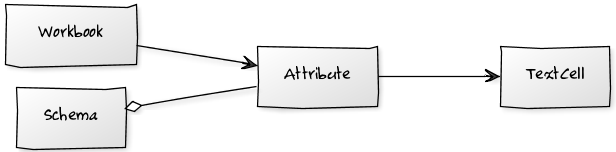
\includegraphics{schema.png}


\subsection{Overheads}
\label{schema:overheads}
A schema depends only on the definitions in {\hyperref[cell:module-cell]{\code{cell}}}.

\begin{Verbatim}[commandchars=\\\{\}]
\PYG{l+s+sd}{\PYGZdq{}\PYGZdq{}\PYGZdq{}stingray.schema \PYGZhy{}\PYGZhy{} Defines an overall Schema of Attributes which can be}
\PYG{l+s+sd}{embedded as a row of a sheet or encoded in a separate sheet.  A}
\PYG{l+s+sd}{schema defines the logical layout of a workbook or flat file.}
\PYG{l+s+sd}{\PYGZdq{}\PYGZdq{}\PYGZdq{}}

\PYG{k+kn}{import} \PYG{n+nn}{datetime}
\PYG{k+kn}{import} \PYG{n+nn}{time}
\PYG{k+kn}{import} \PYG{n+nn}{stingray.cell}
\end{Verbatim}


\subsection{Schema Class}
\label{schema:schema-class}\index{Schema (class in schema)}

\begin{fulllineitems}
\phantomsection\label{schema:schema.Schema}\pysigline{\strong{class }\code{schema.}\bfcode{Schema}}
The core Schema definition is an extension to \code{list}. In addition to
a sequence of attributes, it also has an ``info'' object that's a dictionary
of additional keywords.

The \code{schema.Schema.rows\_as\_dict\_iter()} method uses the sheet's
\code{sheet.Sheet.rows()} iterator to create simple row-as-list values.
These are transformed into the row-as-dict values.  If the attribute names
involve duplicates, then one of the duplicated values will be chosen; the
choice is arbitrary.
\index{info (schema.Schema attribute)}

\begin{fulllineitems}
\phantomsection\label{schema:schema.Schema.info}\pysigline{\bfcode{info}}
Dict of additional information about this schema. Meta-metadata.
For COBOL schema, this includes the source DDE.

\end{fulllineitems}

\index{names (schema.Schema attribute)}

\begin{fulllineitems}
\phantomsection\label{schema:schema.Schema.names}\pysigline{\bfcode{names}}
Attribute names for rows\_as\_dict\_iter()

\end{fulllineitems}


\end{fulllineitems}


\begin{Verbatim}[commandchars=\\\{\}]
\PYG{k}{class} \PYG{n+nc}{Schema}\PYG{p}{(} \PYG{n+nb}{list} \PYG{p}{)}\PYG{p}{:}
    \PYG{l+s+sd}{\PYGZdq{}\PYGZdq{}\PYGZdq{}A Mutable Sequence of attributes.  Order matters.}
\PYG{l+s+sd}{    \PYGZdq{}\PYGZdq{}\PYGZdq{}}
    \PYG{k}{def} \PYG{n+nf}{\PYGZus{}\PYGZus{}init\PYGZus{}\PYGZus{}}\PYG{p}{(} \PYG{n+nb+bp}{self}\PYG{p}{,} \PYG{o}{*}\PYG{n}{attr}\PYG{p}{,} \PYG{o}{*}\PYG{o}{*}\PYG{n}{kw} \PYG{p}{)}\PYG{p}{:}
        \PYG{l+s+sd}{\PYGZdq{}\PYGZdq{}\PYGZdq{}Build a schema from collection of attributes.\PYGZdq{}\PYGZdq{}\PYGZdq{}}
        \PYG{n+nb}{super}\PYG{p}{(}\PYG{p}{)}\PYG{o}{.}\PYG{n}{\PYGZus{}\PYGZus{}init\PYGZus{}\PYGZus{}}\PYG{p}{(} \PYG{n}{attr} \PYG{p}{)}
        \PYG{k}{for} \PYG{n}{p}\PYG{p}{,} \PYG{n}{a} \PYG{o+ow}{in} \PYG{n+nb}{enumerate}\PYG{p}{(} \PYG{n+nb+bp}{self} \PYG{p}{)}\PYG{p}{:}
            \PYG{n}{a}\PYG{o}{.}\PYG{n}{position}\PYG{o}{=} \PYG{n}{p}
        \PYG{n+nb+bp}{self}\PYG{o}{.}\PYG{n}{info}\PYG{o}{=} \PYG{n}{kw}
    \PYG{k}{def} \PYG{n+nf}{\PYGZus{}\PYGZus{}repr\PYGZus{}\PYGZus{}}\PYG{p}{(} \PYG{n+nb+bp}{self} \PYG{p}{)}\PYG{p}{:}
        \PYG{n}{attr\PYGZus{}list}\PYG{o}{=} \PYG{n+nb}{map}\PYG{p}{(} \PYG{n+nb}{repr}\PYG{p}{,} \PYG{n+nb+bp}{self} \PYG{p}{)}
        \PYG{k}{return} \PYG{l+s}{\PYGZdq{}}\PYG{l+s}{Schema( \PYGZob{}0\PYGZcb{} )}\PYG{l+s}{\PYGZdq{}}\PYG{o}{.}\PYG{n}{format}\PYG{p}{(} \PYG{l+s}{\PYGZdq{}}\PYG{l+s}{, }\PYG{l+s}{\PYGZdq{}}\PYG{o}{.}\PYG{n}{join}\PYG{p}{(}\PYG{n}{attr\PYGZus{}list}\PYG{p}{)} \PYG{p}{)}
    \PYG{k}{def} \PYG{n+nf}{rows\PYGZus{}as\PYGZus{}dict\PYGZus{}iter}\PYG{p}{(} \PYG{n+nb+bp}{self}\PYG{p}{,} \PYG{n}{sheet} \PYG{p}{)}\PYG{p}{:}
        \PYG{n+nb+bp}{self}\PYG{o}{.}\PYG{n}{names}\PYG{o}{=} \PYG{n+nb}{tuple}\PYG{p}{(}\PYG{n}{a}\PYG{o}{.}\PYG{n}{name} \PYG{k}{for} \PYG{n}{a} \PYG{o+ow}{in} \PYG{n+nb+bp}{self}\PYG{p}{)}
        \PYG{k}{for} \PYG{n}{r} \PYG{o+ow}{in} \PYG{n}{sheet}\PYG{o}{.}\PYG{n}{rows}\PYG{p}{(}\PYG{p}{)}\PYG{p}{:}
            \PYG{k}{yield} \PYG{n+nb}{dict}\PYG{p}{(}
                \PYG{p}{(}\PYG{n}{a}\PYG{o}{.}\PYG{n}{name}\PYG{p}{,} \PYG{n}{r}\PYG{o}{.}\PYG{n}{cell}\PYG{p}{(}\PYG{n}{a}\PYG{p}{)}\PYG{p}{)} \PYG{k}{for} \PYG{n}{a} \PYG{o+ow}{in} \PYG{n}{sheet}\PYG{o}{.}\PYG{n}{schema} \PYG{p}{)}
    \PYG{k}{def} \PYG{n+nf}{append}\PYG{p}{(} \PYG{n+nb+bp}{self}\PYG{p}{,} \PYG{n}{child} \PYG{p}{)}\PYG{p}{:}
        \PYG{n}{child}\PYG{o}{.}\PYG{n}{position}\PYG{o}{=} \PYG{n+nb}{len}\PYG{p}{(}\PYG{n+nb+bp}{self}\PYG{p}{)}
        \PYG{n+nb}{super}\PYG{p}{(}\PYG{p}{)}\PYG{o}{.}\PYG{n}{append}\PYG{p}{(} \PYG{n}{child} \PYG{p}{)}
\end{Verbatim}

Possibly helpful method to expand a row based on the schema information.

\begin{Verbatim}[commandchars=\\\{\}]
\PYG{k}{def} \PYG{n+nf}{expand}\PYG{p}{(} \PYG{n+nb+bp}{self}\PYG{p}{,} \PYG{n}{aRow} \PYG{p}{)}\PYG{p}{:}
    \PYG{l+s+sd}{\PYGZdq{}\PYGZdq{}\PYGZdq{}Expand each attribute to create a dictionary of cells.\PYGZdq{}\PYGZdq{}\PYGZdq{}}
    \PYG{k}{return} \PYG{n+nb}{dict}\PYG{p}{(} \PYG{p}{(}\PYG{n}{attr}\PYG{o}{.}\PYG{n}{name}\PYG{p}{,} \PYG{n}{aRow}\PYG{o}{.}\PYG{n}{cell}\PYG{p}{(}\PYG{n}{attr}\PYG{p}{)}\PYG{p}{)} \PYG{k}{for} \PYG{n}{attr} \PYG{o+ow}{in} \PYG{n+nb+bp}{self} \PYG{p}{)}
\end{Verbatim}

For parsing COBOL data, we often need to know the total length of the defined schema.
This only works for records without an Occurs Depending On.

\begin{Verbatim}[commandchars=\\\{\}]
\PYG{k}{def} \PYG{n+nf}{lrecl}\PYG{p}{(} \PYG{n+nb+bp}{self} \PYG{p}{)}\PYG{p}{:}
    \PYG{k}{return} \PYG{n+nb}{max}\PYG{p}{(} \PYG{n}{a}\PYG{o}{.}\PYG{n}{offset} \PYG{o}{+} \PYG{n}{a}\PYG{o}{.}\PYG{n}{size} \PYG{k}{for} \PYG{n}{a} \PYG{o+ow}{in} \PYG{n+nb+bp}{self} \PYG{p}{)}
\end{Verbatim}

A Schema needs to handle two common use cases.
\begin{itemize}
\item {} 
Cell values are defined by the physical format. Data can be fetched positionally.
Names map to positions.

\item {} 
Fixed and COBOL.  The cell values are not defined by the physical format, but by an external
schema associated with the {\hyperref[sheet:sheet.Sheet]{\code{sheet.Sheet}}}. Names map to offsets and sizes;
the bytes found there must be converted to Python objects. In the case of
Occurs Depending On (ODO), the offsets depend on both schema and data.

COBOL data may have elements which are invalid, but unused due to application
logic in selecting a proper REDEFINES alias.

\end{itemize}

The simple positional schema isn't really appropriate for all purposes.
For COBOL and fixed format files with external schema, we often
must process things lazily by field name.

This is unlike spreadsheets where we can process all fields eagerly and in order.

\begin{notice}{note}{Todo}

Index by name and path, also.

This will eliminate some complexity in COBOL schema handling where
we create the a ``schema dictionary'' using simple names and path names.
\end{notice}


\subsection{Attribute Class}
\label{schema:attribute-class}\index{Attribute (class in schema)}

\begin{fulllineitems}
\phantomsection\label{schema:schema.Attribute}\pysigline{\strong{class }\code{schema.}\bfcode{Attribute}}
An Attribute definition has a required value of a name and a class that will
be created to hold the data.

Here are the essential attributes of an Attribute.
\index{name (schema.Attribute attribute)}

\begin{fulllineitems}
\phantomsection\label{schema:schema.Attribute.name}\pysigline{\bfcode{name}}
The attribute name. Typically always available for most kinds of schema.

\end{fulllineitems}

\index{create (schema.Attribute attribute)}

\begin{fulllineitems}
\phantomsection\label{schema:schema.Attribute.create}\pysigline{\bfcode{create}}
Cell class to create.  If omitted, the class-level
\code{Attribute.default\_cell} will be used.
By default, this refers to \code{stingray.cell.TextCell}.

\end{fulllineitems}


The additional
values commonly provided by simple fixed format file schemata.
\index{offset (schema.Attribute attribute)}

\begin{fulllineitems}
\phantomsection\label{schema:schema.Attribute.offset}\pysigline{\bfcode{offset}}
Optional offset into a buffer. For simple fixed-layout files,
this is a constant. For COBOL files with Occurs Depending On,
however, this must be a function based on the actual record
being processed.

\end{fulllineitems}

\index{size (schema.Attribute attribute)}

\begin{fulllineitems}
\phantomsection\label{schema:schema.Attribute.size}\pysigline{\bfcode{size}}
Optional size within the buffer.

\end{fulllineitems}

\index{position (schema.Attribute attribute)}

\begin{fulllineitems}
\phantomsection\label{schema:schema.Attribute.position}\pysigline{\bfcode{position}}
Optional sequential position.

\end{fulllineitems}


A subclass might introduce yet more attributes.

\end{fulllineitems}


\begin{Verbatim}[commandchars=\\\{\}]
\PYG{k}{class} \PYG{n+nc}{Attribute}\PYG{p}{:}
    \PYG{l+s+sd}{\PYGZdq{}\PYGZdq{}\PYGZdq{}Essential definition of a single source data element.\PYGZdq{}\PYGZdq{}\PYGZdq{}}
    \PYG{n}{default\PYGZus{}cell}\PYG{o}{=} \PYG{n}{stingray}\PYG{o}{.}\PYG{n}{cell}\PYG{o}{.}\PYG{n}{TextCell}
    \PYG{k}{def} \PYG{n+nf}{\PYGZus{}\PYGZus{}init\PYGZus{}\PYGZus{}}\PYG{p}{(}\PYG{n+nb+bp}{self}\PYG{p}{,} \PYG{n}{name}\PYG{p}{,} \PYG{n}{offset}\PYG{o}{=}\PYG{n+nb+bp}{None}\PYG{p}{,} \PYG{n}{size}\PYG{o}{=}\PYG{n+nb+bp}{None}\PYG{p}{,} \PYG{n}{create}\PYG{o}{=}\PYG{n+nb+bp}{None}\PYG{p}{,} \PYG{n}{position}\PYG{o}{=}\PYG{n+nb+bp}{None}\PYG{p}{,} \PYG{o}{*}\PYG{o}{*}\PYG{n}{kw}\PYG{p}{)}\PYG{p}{:}
        \PYG{l+s+sd}{\PYGZdq{}\PYGZdq{}\PYGZdq{}Build an Attribute.}
\PYG{l+s+sd}{        :param name: The attribute name.}
\PYG{l+s+sd}{        :param offset: Optional offset into a buffer.}
\PYG{l+s+sd}{        :param size: Optional size within the buffer.}
\PYG{l+s+sd}{        :param create: Cell class to create.  If omitted, the class\PYGZhy{}level}
\PYG{l+s+sd}{            :py:data:{}`Attribute.default\PYGZus{}cell{}` will be used.}
\PYG{l+s+sd}{        :param position: Optional sequential position.}
\PYG{l+s+sd}{        \PYGZdq{}\PYGZdq{}\PYGZdq{}}
        \PYG{n+nb+bp}{self}\PYG{o}{.}\PYG{n}{name}\PYG{p}{,} \PYG{n+nb+bp}{self}\PYG{o}{.}\PYG{n}{offset}\PYG{p}{,} \PYG{n+nb+bp}{self}\PYG{o}{.}\PYG{n}{size}\PYG{p}{,} \PYG{n+nb+bp}{self}\PYG{o}{.}\PYG{n}{create}\PYG{p}{,} \PYG{n+nb+bp}{self}\PYG{o}{.}\PYG{n}{position} \PYG{o}{=}\PYGZbs{}
        \PYG{n}{name}\PYG{p}{,} \PYG{n}{offset}\PYG{p}{,} \PYG{n}{size}\PYG{p}{,} \PYG{n}{create}\PYG{p}{,} \PYG{n}{position}
        \PYG{k}{if} \PYG{o+ow}{not} \PYG{n+nb+bp}{self}\PYG{o}{.}\PYG{n}{create}\PYG{p}{:}
            \PYG{n+nb+bp}{self}\PYG{o}{.}\PYG{n}{create}\PYG{o}{=} \PYG{n+nb+bp}{self}\PYG{o}{.}\PYG{n}{default\PYGZus{}cell}
        \PYG{n+nb+bp}{self}\PYG{o}{.}\PYG{n}{\PYGZus{}\PYGZus{}dict\PYGZus{}\PYGZus{}}\PYG{o}{.}\PYG{n}{update}\PYG{p}{(} \PYG{n}{kw} \PYG{p}{)}
    \PYG{k}{def} \PYG{n+nf}{\PYGZus{}\PYGZus{}repr\PYGZus{}\PYGZus{}}\PYG{p}{(} \PYG{n+nb+bp}{self} \PYG{p}{)}\PYG{p}{:}
        \PYG{k}{return} \PYG{l+s}{\PYGZdq{}}\PYG{l+s}{Attribute( name=\PYGZob{}0.name!r\PYGZcb{}, position=\PYGZob{}0.position\PYGZcb{}, offset=\PYGZob{}0.offset\PYGZcb{}, size=\PYGZob{}0.size\PYGZcb{} )}\PYG{l+s}{\PYGZdq{}}\PYG{o}{.}\PYG{n}{format}\PYG{p}{(} \PYG{n+nb+bp}{self} \PYG{p}{)}
\end{Verbatim}

An {\hyperref[schema:schema.Attribute]{\code{schema.Attribute}}} is used by a {\hyperref[workbook/base:workbook.base.Workbook]{\code{workbook.base.Workbook}}} to
extract cell data from a row.

The use case looks like this for a Fixed format workbook.  For other
workbooks, other kinds of conversion functions might be used.

\begin{Verbatim}[commandchars=\\\{\}]
\PYG{k}{def} \PYG{n+nf}{cell}\PYG{p}{(} \PYG{n}{sheet}\PYG{p}{,} \PYG{n}{attribute}\PYG{p}{,} \PYG{n}{data} \PYG{p}{)}\PYG{p}{:}
    \PYG{n}{a}\PYG{o}{=} \PYG{n}{attribute}
    \PYG{k}{return} \PYG{n}{a}\PYG{o}{.}\PYG{n}{create}\PYG{p}{(} \PYG{n}{data}\PYG{p}{[}\PYG{n}{a}\PYG{o}{.}\PYG{n}{offset}\PYG{p}{:}\PYG{n}{a}\PYG{o}{.}\PYG{n}{offset}\PYG{o}{+}\PYG{n}{a}\PYG{o}{.}\PYG{n}{size}\PYG{p}{]}\PYG{p}{,} \PYG{n}{sheet}\PYG{o}{.}\PYG{n}{workbook} \PYG{p}{)}
\end{Verbatim}

The attribute might be declared as follows.
\begin{alltt}
Attribute( name= ``mm-dd-yy'', size= \emph{n}, offset= \emph{m},
    create=SomeCellSubclass )
\end{alltt}


\section{Schema Loader Module -- Load Embedded or External Schema}
\label{schema_loader:module-schema.loader}\label{schema_loader::doc}\label{schema_loader:schema-loader-module-load-embedded-or-external-schema}\label{schema_loader:schema-loader}\index{schema.loader (module)}
A \emph{Schema Loader} loads the attributes of a schema from a source document.
There are a variety of sources.
\begin{itemize}
\item {} 
The first row of a sheet within a workbook.
This version has to be injected into workbook processing
so that the first row is separated from the data rows.

\item {} 
A separate sheet of a workbook.
This version requires a sheet name.

\item {} 
A separate workbook.  This, too, requires a named sheet.

\item {} 
COBOL Code.  We'll set this aside as a subclass
so complex it requires it's own module.

\end{itemize}

A schema loader is paired with a specific kind of {\hyperref[sheet:sheet.Sheet]{\code{sheet.Sheet}}}.

A workbook requires a schema, which requires a schema loader.
A schema loader depends on a meta-workbook.  Ideally that meta-workbook has
an emedded schema, but it may have an external schema, meaning we could have a
meta-schema required load the schema for the application data.  Sheesh.

First, let's hope that doesn't happen.  Second, the circularity is resolved by making it the responsibility of the
the application to handle schema loading.


\subsection{Embedded Schema Use Case}
\label{schema_loader:embedded-schema-use-case}
A {\hyperref[sheet:sheet.EmbeddedSchemaSheet]{\code{sheet.EmbeddedSchemaSheet}}} requires a loader class.
The loader will
\begin{enumerate}
\item {} 
Be built with the sheet as an argument.

\item {} 
Be interrogated for the schema.

\item {} 
Be interrogated for the rows.

\end{enumerate}

The most typical case is the single-header-row case.

In some cases, the loader is actually a
a rather sophisticated parser that paritions the data into the embedded schema
and the data rows.
\begin{alltt}
with Workbook( name ) as wb:
    sheet = self.wb.sheet( `Sheet2',
        stingray.sheet.EmbeddedSchemaSheet,
        loader\_class= stingray.schema.loader.HeadingRowSchemaLoader )

    for row in sheet.rows():
        \emph{process the row}
\end{alltt}


\subsection{External Schema Use Case}
\label{schema_loader:external-schema-use-case}
A {\hyperref[sheet:sheet.ExternalSchemaSheet]{\code{sheet.ExternalSchemaSheet}}} requires a schema.

In the typical case, the external schema file has an emedded meta-schema.
The first row has appropriate column names.
This requires a subclass of {\hyperref[schema_loader:schema.loader.ExternalSchemaLoader]{\code{schema.loader.ExternalSchemaLoader}}} to properly map the names that were found onto the attributes of the {\hyperref[schema:schema.Attribute]{\code{schema.Attribute}}} class.

When the embedded meta-schema has unusual names, then a builder must be defined
to map the names that are found in the schema and build an {\hyperref[schema:schema.Attribute]{\code{schema.Attribute}}} instance.

\begin{Verbatim}[commandchars=\\\{\}]
\PYG{k}{with} \PYG{n}{open\PYGZus{}workbook}\PYG{p}{(} \PYG{n}{schema\PYGZus{}name} \PYG{p}{)} \PYG{k}{as} \PYG{n}{schema\PYGZus{}wb}\PYG{p}{:}
    \PYG{n}{esl}\PYG{o}{=} \PYG{n}{stingray}\PYG{o}{.}\PYG{n}{schema}\PYG{o}{.}\PYG{n}{loader}\PYG{o}{.}\PYG{n}{ExternalSchemaLoader}\PYG{p}{(} \PYG{n}{schema\PYGZus{}wb}\PYG{p}{,} \PYG{l+s}{\PYGZdq{}}\PYG{l+s}{Schema}\PYG{l+s}{\PYGZdq{}} \PYG{p}{)}
    \PYG{n}{schema}\PYG{o}{=} \PYG{n}{esl}\PYG{o}{.}\PYG{n}{schema}\PYG{p}{(}\PYG{p}{)}
\PYG{k}{with} \PYG{n}{Workbook}\PYG{p}{(} \PYG{n}{name}\PYG{p}{,} \PYG{n}{schema}\PYG{o}{=}\PYG{n}{schema} \PYG{p}{)} \PYG{k}{as} \PYG{n}{wb}\PYG{p}{:}
    \PYG{n}{sheet} \PYG{o}{=} \PYG{n+nb+bp}{self}\PYG{o}{.}\PYG{n}{wb}\PYG{o}{.}\PYG{n}{sheet}\PYG{p}{(} \PYG{l+s}{\PYGZsq{}}\PYG{l+s}{Sheet2}\PYG{l+s}{\PYGZsq{}}\PYG{p}{,}
        \PYG{n}{stingray}\PYG{o}{.}\PYG{n}{sheet}\PYG{o}{.}\PYG{n}{ExternalSchemaSheet}\PYG{p}{,}
        \PYG{n}{schema}\PYG{o}{=} \PYG{n}{schema} \PYG{p}{)}
    \PYG{n}{counts}\PYG{o}{=} \PYG{n}{process\PYGZus{}sheet}\PYG{p}{(} \PYG{n}{sheet} \PYG{p}{)}
    \PYG{n}{pprint}\PYG{o}{.}\PYG{n}{pprint}\PYG{p}{(} \PYG{n}{counts} \PYG{p}{)}
\end{Verbatim}


\subsection{Manual Schema Use Case}
\label{schema_loader:manual-schema-use-case}
Also, a manually-defined {\hyperref[schema:schema.Schema]{\code{schema.Schema}}} can be built rather than being loaded.

\begin{Verbatim}[commandchars=\\\{\}]
\PYG{n}{schema}\PYG{o}{=} \PYG{n}{stingray}\PYG{o}{.}\PYG{n}{schema}\PYG{o}{.}\PYG{n}{Schema}\PYG{p}{(}
    \PYG{n}{stingray}\PYG{o}{.}\PYG{n}{schema}\PYG{o}{.}\PYG{n}{Attribute}\PYG{p}{(} \PYG{n}{name}\PYG{o}{=}\PYG{l+s}{\PYGZsq{}}\PYG{l+s}{Column \PYGZsh{}1}\PYG{l+s}{\PYGZsq{}} \PYG{p}{)}\PYG{p}{,}
    \PYG{n}{stingray}\PYG{o}{.}\PYG{n}{schema}\PYG{o}{.}\PYG{n}{Attribute}\PYG{p}{(} \PYG{n}{name}\PYG{o}{=}\PYG{l+s}{\PYGZsq{}}\PYG{l+s}{Key}\PYG{l+s}{\PYGZsq{}} \PYG{p}{)}\PYG{p}{,}
    \PYG{n}{stingray}\PYG{o}{.}\PYG{n}{schema}\PYG{o}{.}\PYG{n}{Attribute}\PYG{p}{(} \PYG{n}{name}\PYG{o}{=}\PYG{l+s}{\PYGZsq{}}\PYG{l+s}{Value}\PYG{l+s}{\PYGZsq{}} \PYG{p}{)}\PYG{p}{,}
    \PYG{n}{stingray}\PYG{o}{.}\PYG{n}{schema}\PYG{o}{.}\PYG{n}{Attribute}\PYG{p}{(} \PYG{n}{name}\PYG{o}{=}\PYG{l+s}{\PYGZsq{}}\PYG{l+s}{Etc.}\PYG{l+s}{\PYGZsq{}} \PYG{p}{)}\PYG{p}{,}
\PYG{p}{)}
\end{Verbatim}


\subsection{Model}
\label{schema_loader:model}
\begin{Verbatim}[commandchars=\\\{\}]
http://yuml.me/diagram/scruffy;/class/
\PYGZsh{}schema\PYGZhy{}loader,
[Schema]\PYGZlt{}\PYGZgt{}\PYGZhy{}[Attribute],
[SchemaLoader]\PYGZhy{}builds\PYGZhy{}\PYGZgt{}[Schema],
[SchemaLoader]\PYGZca{}[HeadingRowSchemaLoader],
[SchemaLoader]\PYGZca{}[ExternalSchemaLoader],
[ExternalSchemaLoader]\PYGZhy{}reads\PYGZhy{}\PYGZgt{}[Workbook],
[HeadingRowSchemaLoader]\PYGZhy{}reads\PYGZhy{}\PYGZgt{}[Sheet].
\end{Verbatim}

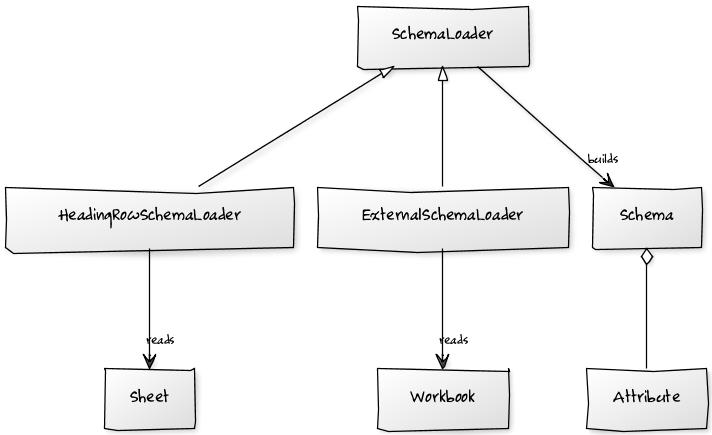
\includegraphics[width=6in]{schema_loader.png}


\subsection{Overheads}
\label{schema_loader:overheads}
We depend on {\hyperref[schema:module-schema]{\code{schema}}}, {\hyperref[cell:module-cell]{\code{cell}}} and {\hyperref[sheet:module-sheet]{\code{sheet}}}.

\begin{Verbatim}[commandchars=\\\{\}]
\PYG{l+s+sd}{\PYGZdq{}\PYGZdq{}\PYGZdq{}stingray.schema.loader \PYGZhy{}\PYGZhy{} Loads a Schema from a row of a Sheet or}
\PYG{l+s+sd}{from a separate Sheet.  This is extended to load COBOL schema}
\PYG{l+s+sd}{from DDE files.}
\PYG{l+s+sd}{\PYGZdq{}\PYGZdq{}\PYGZdq{}}

\PYG{k+kn}{from} \PYG{n+nn}{stingray.schema} \PYG{k+kn}{import} \PYG{n}{Schema}\PYG{p}{,} \PYG{n}{Attribute}
\PYG{k+kn}{import} \PYG{n+nn}{stingray.cell}
\PYG{k+kn}{import} \PYG{n+nn}{stingray.sheet}
\PYG{k+kn}{import} \PYG{n+nn}{warnings}
\end{Verbatim}


\subsection{No Schema Exception}
\label{schema_loader:no-schema-exception}
In some circumstances, we can't load a schema. The most common situation
is a {\hyperref[schema_loader:schema.loader.HeadingRowSchemaLoader]{\code{HeadingRowSchemaLoader}}} which is applied to an empty workbook sheet.
No rows means no schema.

\begin{Verbatim}[commandchars=\\\{\}]
\PYG{k}{class} \PYG{n+nc}{NoSchemaFound}\PYG{p}{(} \PYG{n+ne}{Exception} \PYG{p}{)}\PYG{p}{:}
    \PYG{k}{pass}
\end{Verbatim}

The default behavior is to simply write a warning for an empty sheet.
The lack of a schema means there's no data, also, and 99\% of the time, silently ignoring
an empty sheet is desirable.


\subsection{Schema Loader}
\label{schema_loader:id1}\index{SchemaLoader (class in schema.loader)}

\begin{fulllineitems}
\phantomsection\label{schema_loader:schema.loader.SchemaLoader}\pysigline{\strong{class }\code{schema.loader.}\bfcode{SchemaLoader}}
A Schema Loader has one mandatory contract: It must load the schema.

A subclass may add a second contract, For example,
an embedded schema loader will also return the non-schema rows.
\index{sheet (schema.loader.SchemaLoader attribute)}

\begin{fulllineitems}
\phantomsection\label{schema_loader:schema.loader.SchemaLoader.sheet}\pysigline{\bfcode{sheet}}
The \code{Sheet} associated with this schema.

\end{fulllineitems}

\index{row\_iter (schema.loader.SchemaLoader attribute)}

\begin{fulllineitems}
\phantomsection\label{schema_loader:schema.loader.SchemaLoader.row_iter}\pysigline{\bfcode{row\_iter}}
An iterator over the rows of this sheet; used to pick rows that
belong to the header, separate from the rows that belong to data.

\end{fulllineitems}


\end{fulllineitems}


\begin{Verbatim}[commandchars=\\\{\}]
\PYG{k}{class} \PYG{n+nc}{SchemaLoader}\PYG{p}{:}
    \PYG{l+s+sd}{\PYGZdq{}\PYGZdq{}\PYGZdq{}Locate schema information.  Subclasses handle}
\PYG{l+s+sd}{    all of the variations on schema representation.}
\PYG{l+s+sd}{    \PYGZdq{}\PYGZdq{}\PYGZdq{}}
    \PYG{k}{def} \PYG{n+nf}{\PYGZus{}\PYGZus{}init\PYGZus{}\PYGZus{}}\PYG{p}{(} \PYG{n+nb+bp}{self}\PYG{p}{,} \PYG{n}{sheet} \PYG{p}{)}\PYG{p}{:}
        \PYG{l+s+sd}{\PYGZdq{}\PYGZdq{}\PYGZdq{}A simple :py:class:{}`Sheet{}` instance.\PYGZdq{}\PYGZdq{}\PYGZdq{}}
        \PYG{n+nb+bp}{self}\PYG{o}{.}\PYG{n}{sheet}\PYG{o}{=} \PYG{n}{sheet}
        \PYG{n+nb+bp}{self}\PYG{o}{.}\PYG{n}{row\PYGZus{}iter}\PYG{o}{=} \PYG{n+nb}{iter}\PYG{p}{(} \PYG{n+nb+bp}{self}\PYG{o}{.}\PYG{n}{sheet}\PYG{o}{.}\PYG{n}{rows}\PYG{p}{(}\PYG{p}{)} \PYG{p}{)}
    \PYG{k}{def} \PYG{n+nf}{schema}\PYG{p}{(} \PYG{n+nb+bp}{self} \PYG{p}{)}\PYG{p}{:}
        \PYG{l+s+sd}{\PYGZdq{}\PYGZdq{}\PYGZdq{}Scan the sheet to get the schema.}
\PYG{l+s+sd}{        :return: a :py:class:{}`Schema{}` object.\PYGZdq{}\PYGZdq{}\PYGZdq{}}
        \PYG{k}{return} \PYG{n+nb+bp}{NotImplemented}
    \PYG{k}{def} \PYG{n+nf}{rows}\PYG{p}{(} \PYG{n+nb+bp}{self} \PYG{p}{)}\PYG{p}{:}
        \PYG{l+s+sd}{\PYGZdq{}\PYGZdq{}\PYGZdq{}Iterate all (or remaining) rows.\PYGZdq{}\PYGZdq{}\PYGZdq{}}
        \PYG{k}{return} \PYG{n+nb+bp}{self}\PYG{o}{.}\PYG{n}{row\PYGZus{}iter}
\end{Verbatim}


\subsection{Embedded Schema Loader}
\label{schema_loader:embedded-schema-loader}\index{HeadingRowSchemaLoader (class in schema.loader)}

\begin{fulllineitems}
\phantomsection\label{schema_loader:schema.loader.HeadingRowSchemaLoader}\pysigline{\strong{class }\code{schema.loader.}\bfcode{HeadingRowSchemaLoader}}
In many cases, the schema is first-row column titles or something similar.
As we noted above, \code{csv.DictReader} supports this simple case.

All other cases have to be handled with something a bit more sophisticated.
The {\hyperref[schema_loader:schema.loader.SchemaLoader]{\code{schema.loader.SchemaLoader}}} can be further subclassed to provide for more
complex schema definitions buried in the rows of a sheet.

This means that we must make the schema parsing an application-provided
plug-in that the Workbook uses when instantiating each Sheet.

\end{fulllineitems}


\begin{Verbatim}[commandchars=\\\{\}]
\PYG{k}{class} \PYG{n+nc}{HeadingRowSchemaLoader}\PYG{p}{(} \PYG{n}{SchemaLoader} \PYG{p}{)}\PYG{p}{:}
    \PYG{l+s+sd}{\PYGZdq{}\PYGZdq{}\PYGZdq{}Read just the first row of a sheet to get embedded}
\PYG{l+s+sd}{    schema information.\PYGZdq{}\PYGZdq{}\PYGZdq{}}
    \PYG{k}{def} \PYG{n+nf}{schema}\PYG{p}{(} \PYG{n+nb+bp}{self} \PYG{p}{)}\PYG{p}{:}
        \PYG{l+s+sd}{\PYGZdq{}\PYGZdq{}\PYGZdq{}Try to get the schema from row one.  Remaining rows are data.}
\PYG{l+s+sd}{        If the sheet is empty, emit a warning and return {}`{}`None{}`{}`.}
\PYG{l+s+sd}{        \PYGZdq{}\PYGZdq{}\PYGZdq{}}
        \PYG{k}{try}\PYG{p}{:}
            \PYG{n}{row\PYGZus{}1}\PYG{o}{=} \PYG{n+nb}{next}\PYG{p}{(} \PYG{n+nb+bp}{self}\PYG{o}{.}\PYG{n}{row\PYGZus{}iter} \PYG{p}{)}
            \PYG{n}{attributes} \PYG{o}{=} \PYG{p}{(}
                \PYG{n+nb}{dict}\PYG{p}{(}\PYG{n}{name}\PYG{o}{=}\PYG{n}{c}\PYG{o}{.}\PYG{n}{to\PYGZus{}str}\PYG{p}{(}\PYG{p}{)}\PYG{p}{)} \PYG{k}{for} \PYG{n}{c} \PYG{o+ow}{in} \PYG{n}{row\PYGZus{}1}
            \PYG{p}{)}
            \PYG{n}{schema} \PYG{o}{=} \PYG{n}{Schema}\PYG{p}{(}
                \PYG{o}{*}\PYG{p}{(}\PYG{n}{Attribute}\PYG{p}{(}\PYG{o}{*}\PYG{o}{*}\PYG{n}{col}\PYG{p}{)} \PYG{k}{for} \PYG{n}{col} \PYG{o+ow}{in} \PYG{n}{attributes}\PYG{p}{)}
            \PYG{p}{)}
            \PYG{k}{return} \PYG{n}{schema}
        \PYG{k}{except} \PYG{n+ne}{StopIteration}\PYG{p}{:}
            \PYG{n}{warnings}\PYG{o}{.}\PYG{n}{warn}\PYG{p}{(} \PYG{l+s}{\PYGZdq{}}\PYG{l+s}{Empty sheet: no schema present}\PYG{l+s}{\PYGZdq{}} \PYG{p}{)}
\end{Verbatim}

We'll open a {\hyperref[sheet:sheet.Sheet]{\code{sheet.Sheet}}} with a specific loader.

\begin{Verbatim}[commandchars=\\\{\}]
\PYG{n}{sheet}\PYG{o}{=} \PYG{n}{stingray}\PYG{o}{.}\PYG{n}{sheet}\PYG{o}{.}\PYG{n}{EmbeddedSchemaSheet}\PYG{p}{(}
    \PYG{n+nb+bp}{self}\PYG{o}{.}\PYG{n}{wb}\PYG{p}{,} \PYG{l+s}{\PYGZsq{}}\PYG{l+s}{The\PYGZus{}Name}\PYG{l+s}{\PYGZsq{}}\PYG{p}{,}
    \PYG{n}{loader\PYGZus{}class}\PYG{o}{=}\PYG{n}{HeadingRowSchemaLoader} \PYG{p}{)}
\end{Verbatim}
\index{NonBlankHeadingRowSchemaLoader (class in schema.loader)}

\begin{fulllineitems}
\phantomsection\label{schema_loader:schema.loader.NonBlankHeadingRowSchemaLoader}\pysigline{\strong{class }\code{schema.loader.}\bfcode{NonBlankHeadingRowSchemaLoader}}
In many cases, we'd like to suppress the empty rows that are an inevitable feature of workbook sheets.

Note that this doesn't work well for COBOL
or Fixed format files, since an ``empty'' row may be difficult to discern.

\end{fulllineitems}


\begin{Verbatim}[commandchars=\\\{\}]
\PYG{k}{class} \PYG{n+nc}{NonBlankHeadingRowSchemaLoader}\PYG{p}{(} \PYG{n}{HeadingRowSchemaLoader} \PYG{p}{)}\PYG{p}{:}
    \PYG{k}{def} \PYG{n+nf}{\PYGZus{}\PYGZus{}init\PYGZus{}\PYGZus{}}\PYG{p}{(} \PYG{n+nb+bp}{self}\PYG{p}{,} \PYG{n}{sheet} \PYG{p}{)}\PYG{p}{:}
        \PYG{l+s+sd}{\PYGZdq{}\PYGZdq{}\PYGZdq{}A simple :py:class:{}`Sheet{}` instance.\PYGZdq{}\PYGZdq{}\PYGZdq{}}
        \PYG{n+nb+bp}{self}\PYG{o}{.}\PYG{n}{sheet}\PYG{o}{=} \PYG{n}{sheet}
        \PYG{n+nb+bp}{self}\PYG{o}{.}\PYG{n}{row\PYGZus{}iter}\PYG{o}{=} \PYG{n+nb+bp}{self}\PYG{o}{.}\PYG{n}{non\PYGZus{}blank}\PYG{p}{(} \PYG{n+nb+bp}{self}\PYG{o}{.}\PYG{n}{sheet}\PYG{o}{.}\PYG{n}{rows}\PYG{p}{(}\PYG{p}{)} \PYG{p}{)}
    \PYG{k}{def} \PYG{n+nf}{non\PYGZus{}blank}\PYG{p}{(} \PYG{n+nb+bp}{self}\PYG{p}{,} \PYG{n}{rows} \PYG{p}{)}\PYG{p}{:}
        \PYG{k}{for} \PYG{n}{r} \PYG{o+ow}{in} \PYG{n}{rows}\PYG{p}{:}
            \PYG{k}{if} \PYG{n+nb}{all}\PYG{p}{(} \PYG{n}{c}\PYG{o}{.}\PYG{n}{is\PYGZus{}empty}\PYG{p}{(}\PYG{p}{)} \PYG{k}{for} \PYG{n}{c} \PYG{o+ow}{in} \PYG{n}{r} \PYG{p}{)}\PYG{p}{:}
                \PYG{k}{continue}
            \PYG{k}{yield} \PYG{n}{r}
\end{Verbatim}


\subsection{External Schema Loader}
\label{schema_loader:external-schema-loader}\index{ExternalSchemaLoader (class in schema.loader)}

\begin{fulllineitems}
\phantomsection\label{schema_loader:schema.loader.ExternalSchemaLoader}\pysigline{\strong{class }\code{schema.loader.}\bfcode{ExternalSchemaLoader}}
In some cases, the data workbook is described by a separate schema workbook, or a separate
sheet within the data workbook.  In these cases, the other sheet (or file) must be
parsed to locate schema information.

In the case of a fixed format file, we must examine a separate
file to load schema information.  This additional schems file may be in
COBOL notation, leading to a more complex parser.  See {\hyperref[cobol_loader:cobol-loader]{\emph{COBOL Loader Module -- Parse COBOL Source to Load a Schema}}}.

The layout of the schema, of course, will be highly variable,
so the ``meta-schema'' must be adjusted to the actual file.

Note, also, that the schema loader is -- itself -- a typical of schema-based reader.  It has a number of common features.
\begin{enumerate}
\item {} 
A dictionary-based ``builder'', {\hyperref[schema_loader:schema.loader.ExternalSchemaLoader.build_attr]{\code{schema.loader.ExternalSchemaLoader.build\_attr()}}}, to handle Logical Layout.
This transforms the input ``raw'' dictionary of {\hyperref[cell:cell.Cell]{\code{cell.Cell}}} instances to an application dictionary of proper Python objects.
See {\hyperref[developer:developer]{\emph{The Stingray Developer's Guide}}}.

\item {} 
An iterator, {\hyperref[schema_loader:schema.loader.ExternalSchemaLoader.attr_dict_iter]{\code{schema.loader.ExternalSchemaLoader.attr\_dict\_iter()}}},
that provides ``raw'' dictionaries from each row (based on the schema) to the
builder to create application dictionaries.

\item {} 
The overall function,
{\hyperref[schema_loader:schema.loader.ExternalSchemaLoader.schema]{\code{schema.loader.ExternalSchemaLoader.schema()}}},
that iterates over application objects built from application dictionaries.

\end{enumerate}
\index{workbook (schema.loader.ExternalSchemaLoader attribute)}

\begin{fulllineitems}
\phantomsection\label{schema_loader:schema.loader.ExternalSchemaLoader.workbook}\pysigline{\bfcode{workbook}}
The overall Workbook that we're parsing to locate schema information.

\end{fulllineitems}

\index{Sheet (schema.loader.ExternalSchemaLoader attribute)}

\begin{fulllineitems}
\phantomsection\label{schema_loader:schema.loader.ExternalSchemaLoader.Sheet}\pysigline{\bfcode{Sheet}}
A specific sheet within that workbook.

\end{fulllineitems}


\end{fulllineitems}


\begin{Verbatim}[commandchars=\\\{\}]
\PYG{k}{class} \PYG{n+nc}{ExternalSchemaLoader}\PYG{p}{(} \PYG{n}{SchemaLoader} \PYG{p}{)}\PYG{p}{:}
    \PYG{l+s+sd}{\PYGZdq{}\PYGZdq{}\PYGZdq{}Open a workbook file in a well\PYGZhy{}known format.}
\PYG{l+s+sd}{    Build a schema with attribute name, offset, size  and type}
\PYG{l+s+sd}{    information.  The type is a string that names the}
\PYG{l+s+sd}{    type of cell to create.}

\PYG{l+s+sd}{    The meta\PYGZhy{}schema must be embedded as the first line of the schema sheet.}

\PYG{l+s+sd}{    The assumed meta\PYGZhy{}schema is the following::}

\PYG{l+s+sd}{        Schema(}
\PYG{l+s+sd}{            Attribute(\PYGZdq{}name\PYGZdq{},create=\PYGZdq{}TextCell\PYGZdq{}),}
\PYG{l+s+sd}{            Attribute(\PYGZdq{}offset\PYGZdq{},create=\PYGZdq{}NumberCell\PYGZdq{}),}
\PYG{l+s+sd}{            Attribute(\PYGZdq{}size\PYGZdq{},create=\PYGZdq{}NumberCell\PYGZdq{}),}
\PYG{l+s+sd}{            Attribute(\PYGZdq{}type\PYGZdq{},create=\PYGZdq{}TextCell\PYGZdq{}),}
\PYG{l+s+sd}{        )}

\PYG{l+s+sd}{    If the meta\PYGZhy{}schema has different names, then a subclass with}
\PYG{l+s+sd}{    a different :py:meth:{}`build\PYGZus{}attr{}` is required to map the actual}
\PYG{l+s+sd}{    source columns to the attributes of a :py:class:{}`Attribute{}`.}

\PYG{l+s+sd}{    Offsets are typically 1\PYGZhy{}based.}
\PYG{l+s+sd}{    \PYGZdq{}\PYGZdq{}\PYGZdq{}}
    \PYG{k}{def} \PYG{n+nf}{\PYGZus{}\PYGZus{}init\PYGZus{}\PYGZus{}}\PYG{p}{(} \PYG{n+nb+bp}{self}\PYG{p}{,} \PYG{n}{workbook}\PYG{p}{,} \PYG{n}{sheet\PYGZus{}name}\PYG{o}{=}\PYG{l+s}{\PYGZsq{}}\PYG{l+s}{Sheet1}\PYG{l+s}{\PYGZsq{}} \PYG{p}{)}\PYG{p}{:}
        \PYG{n+nb+bp}{self}\PYG{o}{.}\PYG{n}{workbook}\PYG{p}{,} \PYG{n+nb+bp}{self}\PYG{o}{.}\PYG{n}{sheet\PYGZus{}name} \PYG{o}{=} \PYG{n}{workbook}\PYG{p}{,} \PYG{n}{sheet\PYGZus{}name}
        \PYG{n+nb+bp}{self}\PYG{o}{.}\PYG{n}{sheet}\PYG{o}{=} \PYG{n+nb+bp}{self}\PYG{o}{.}\PYG{n}{workbook}\PYG{o}{.}\PYG{n}{sheet}\PYG{p}{(} \PYG{n+nb+bp}{self}\PYG{o}{.}\PYG{n}{sheet\PYGZus{}name}\PYG{p}{,} \PYG{n}{stingray}\PYG{o}{.}\PYG{n}{sheet}\PYG{o}{.}\PYG{n}{EmbeddedSchemaSheet}\PYG{p}{,}
        \PYG{n}{loader\PYGZus{}class}\PYG{o}{=} \PYG{n}{HeadingRowSchemaLoader} \PYG{p}{)}
\end{Verbatim}
\index{build\_attr() (schema.loader.ExternalSchemaLoader method)}

\begin{fulllineitems}
\phantomsection\label{schema_loader:schema.loader.ExternalSchemaLoader.build_attr}\pysiglinewithargsret{\code{ExternalSchemaLoader.}\bfcode{build\_attr}}{\emph{row}}{}
There's potential for a great deal of variability in schema definition.
Consequently, this \code{build\_attr} method is merely a sample that
covers one common case.

\end{fulllineitems}


\begin{Verbatim}[commandchars=\\\{\}]
\PYG{n}{base}\PYG{o}{=} \PYG{l+m+mi}{1}
\PYG{n}{type\PYGZus{}to\PYGZus{}cell} \PYG{o}{=} \PYG{p}{\PYGZob{}}
    \PYG{l+s}{\PYGZsq{}}\PYG{l+s}{text}\PYG{l+s}{\PYGZsq{}}\PYG{p}{:} \PYG{l+s}{\PYGZdq{}}\PYG{l+s}{TextCell}\PYG{l+s}{\PYGZdq{}}\PYG{p}{,}
    \PYG{l+s}{\PYGZsq{}}\PYG{l+s}{number}\PYG{l+s}{\PYGZsq{}}\PYG{p}{:} \PYG{l+s}{\PYGZdq{}}\PYG{l+s}{NumberCell}\PYG{l+s}{\PYGZdq{}}\PYG{p}{,}
    \PYG{l+s}{\PYGZsq{}}\PYG{l+s}{date}\PYG{l+s}{\PYGZsq{}}\PYG{p}{:} \PYG{l+s}{\PYGZdq{}}\PYG{l+s}{DateCell}\PYG{l+s}{\PYGZdq{}}\PYG{p}{,}
    \PYG{l+s}{\PYGZsq{}}\PYG{l+s}{boolean}\PYG{l+s}{\PYGZsq{}}\PYG{p}{:} \PYG{l+s}{\PYGZdq{}}\PYG{l+s}{BooleanCell}\PYG{l+s}{\PYGZdq{}}\PYG{p}{,}
    \PYG{p}{\PYGZcb{}}
\PYG{n+nd}{@staticmethod}
\PYG{k}{def} \PYG{n+nf}{build\PYGZus{}attr}\PYG{p}{(} \PYG{n}{row} \PYG{p}{)}\PYG{p}{:}
    \PYG{l+s+sd}{\PYGZdq{}\PYGZdq{}\PYGZdq{}Build application dictionary from raw dictionary.}
\PYG{l+s+sd}{    \PYGZdq{}\PYGZdq{}\PYGZdq{}}
    \PYG{k}{try}\PYG{p}{:}
        \PYG{n}{offset}\PYG{o}{=} \PYG{n}{row}\PYG{p}{[}\PYG{l+s}{\PYGZsq{}}\PYG{l+s}{offset}\PYG{l+s}{\PYGZsq{}}\PYG{p}{]}\PYG{o}{.}\PYG{n}{to\PYGZus{}int}\PYG{p}{(}\PYG{p}{)}\PYG{o}{\PYGZhy{}}\PYG{n}{ExternalSchemaLoader}\PYG{o}{.}\PYG{n}{base}
    \PYG{k}{except} \PYG{n+ne}{KeyError}\PYG{p}{:}
        \PYG{n}{offset}\PYG{o}{=} \PYG{n+nb+bp}{None}
    \PYG{k}{try}\PYG{p}{:}
        \PYG{n}{size}\PYG{o}{=} \PYG{n}{row}\PYG{p}{[}\PYG{l+s}{\PYGZsq{}}\PYG{l+s}{size}\PYG{l+s}{\PYGZsq{}}\PYG{p}{]}\PYG{o}{.}\PYG{n}{to\PYGZus{}int}\PYG{p}{(}\PYG{p}{)}
    \PYG{k}{except} \PYG{n+ne}{KeyError}\PYG{p}{:}
        \PYG{n}{size}\PYG{o}{=} \PYG{n+nb+bp}{None}
    \PYG{k}{try}\PYG{p}{:}
        \PYG{n}{type\PYGZus{}name}\PYG{o}{=} \PYG{n}{row}\PYG{p}{[}\PYG{l+s}{\PYGZsq{}}\PYG{l+s}{type}\PYG{l+s}{\PYGZsq{}}\PYG{p}{]}\PYG{o}{.}\PYG{n}{to\PYGZus{}str}\PYG{p}{(}\PYG{p}{)}
        \PYG{n}{create}\PYG{o}{=} \PYG{n}{ExternalSchemaLoader}\PYG{o}{.}\PYG{n}{type\PYGZus{}to\PYGZus{}cell}\PYG{p}{[}\PYG{n}{type\PYGZus{}name}\PYG{p}{]}
    \PYG{k}{except} \PYG{n+ne}{KeyError}\PYG{p}{:}
        \PYG{n}{create}\PYG{o}{=} \PYG{n}{stingray}\PYG{o}{.}\PYG{n}{cell}\PYG{o}{.}\PYG{n}{TextCell}
    \PYG{k}{return} \PYG{n+nb}{dict}\PYG{p}{(}
        \PYG{n}{name}\PYG{o}{=} \PYG{n}{row}\PYG{p}{[}\PYG{l+s}{\PYGZsq{}}\PYG{l+s}{name}\PYG{l+s}{\PYGZsq{}}\PYG{p}{]}\PYG{o}{.}\PYG{n}{to\PYGZus{}str}\PYG{p}{(}\PYG{p}{)}\PYG{p}{,}
        \PYG{n}{offset}\PYG{o}{=} \PYG{n}{offset}\PYG{p}{,}
        \PYG{n}{size}\PYG{o}{=} \PYG{n}{size}\PYG{p}{,}
        \PYG{n}{create}\PYG{o}{=} \PYG{n}{create}\PYG{p}{,}
    \PYG{p}{)}
\end{Verbatim}

Schema loading involves a process of
\begin{enumerate}
\item {} 
Iterating through the source rows as dictionaries.
\begin{itemize}
\item {} 
Build each raw row as a source dictionary.

\item {} 
Build an standardized attr dictionary from the source dictionary.
This mapping, implemented by {\hyperref[schema_loader:schema.loader.ExternalSchemaLoader.build_attr]{\code{schema.loader.ExternalSchemaLoader.build\_attr()}}}
is subject to a great deal of change without notice.

\end{itemize}

\item {} 
Building each {\hyperref[schema:schema.Attribute]{\code{schema.Attribute}}} from the dictionary.

\end{enumerate}
\index{attr\_dict\_iter() (schema.loader.ExternalSchemaLoader method)}

\begin{fulllineitems}
\phantomsection\label{schema_loader:schema.loader.ExternalSchemaLoader.attr_dict_iter}\pysiglinewithargsret{\code{ExternalSchemaLoader.}\bfcode{attr\_dict\_iter}}{\emph{sheet}}{}
Iterate over application dicts based on raw dicts built by the schema of the sheet.

\end{fulllineitems}


\begin{Verbatim}[commandchars=\\\{\}]
\PYG{k}{def} \PYG{n+nf}{attr\PYGZus{}dict\PYGZus{}iter}\PYG{p}{(} \PYG{n+nb+bp}{self}\PYG{p}{,} \PYG{n}{sheet} \PYG{p}{)}\PYG{p}{:}
    \PYG{l+s+sd}{\PYGZdq{}\PYGZdq{}\PYGZdq{}Iterate over application dicts based on raw dicts}
\PYG{l+s+sd}{    built by the schema of the sheet.\PYGZdq{}\PYGZdq{}\PYGZdq{}}
    \PYG{k}{return} \PYG{p}{(}
        \PYG{n}{ExternalSchemaLoader}\PYG{o}{.}\PYG{n}{build\PYGZus{}attr}\PYG{p}{(}\PYG{n}{r}\PYG{p}{)}
        \PYG{k}{for} \PYG{n}{r} \PYG{o+ow}{in} \PYG{n}{sheet}\PYG{o}{.}\PYG{n}{schema}\PYG{o}{.}\PYG{n}{rows\PYGZus{}as\PYGZus{}dict\PYGZus{}iter}\PYG{p}{(}\PYG{n}{sheet}\PYG{p}{)}
    \PYG{p}{)}
\end{Verbatim}
\index{schema() (schema.loader.ExternalSchemaLoader method)}

\begin{fulllineitems}
\phantomsection\label{schema_loader:schema.loader.ExternalSchemaLoader.schema}\pysiglinewithargsret{\code{ExternalSchemaLoader.}\bfcode{schema}}{}{}
Scan a file to get the schema.
\begin{quote}\begin{description}
\item[{Returns}] \leavevmode
a \code{Schema} object

\end{description}\end{quote}

\end{fulllineitems}


\begin{Verbatim}[commandchars=\\\{\}]
\PYG{k}{def} \PYG{n+nf}{schema}\PYG{p}{(} \PYG{n+nb+bp}{self} \PYG{p}{)}\PYG{p}{:}
    \PYG{l+s+sd}{\PYGZdq{}\PYGZdq{}\PYGZdq{}Scan a file to get the schema.}
\PYG{l+s+sd}{    :return: a :py:class:{}`Schema{}` object.\PYGZdq{}\PYGZdq{}\PYGZdq{}}
    \PYG{n+nb+bp}{self}\PYG{o}{.}\PYG{n}{row\PYGZus{}iter}\PYG{o}{=} \PYG{n+nb}{iter}\PYG{p}{(} \PYG{p}{[}\PYG{p}{]} \PYG{p}{)}
    \PYG{n}{source\PYGZus{}dict} \PYG{o}{=} \PYG{n+nb+bp}{self}\PYG{o}{.}\PYG{n}{attr\PYGZus{}dict\PYGZus{}iter}\PYG{p}{(} \PYG{n+nb+bp}{self}\PYG{o}{.}\PYG{n}{sheet} \PYG{p}{)}
    \PYG{n}{schema}\PYG{o}{=} \PYG{n}{Schema}\PYG{p}{(}
        \PYG{o}{*}\PYG{p}{(}\PYG{n}{Attribute}\PYG{p}{(}\PYG{o}{*}\PYG{o}{*}\PYG{n}{row}\PYG{p}{)} \PYG{k}{for} \PYG{n}{row} \PYG{o+ow}{in} \PYG{n}{source\PYGZus{}dict}\PYG{p}{)}
    \PYG{p}{)}
    \PYG{k}{return} \PYG{n}{schema}
\end{Verbatim}


\subsection{Worst-Case Loader}
\label{schema_loader:worst-case-loader}\index{BareExternalSchemaLoader (class in schema.loader)}

\begin{fulllineitems}
\phantomsection\label{schema_loader:schema.loader.BareExternalSchemaLoader}\pysigline{\strong{class }\code{schema.loader.}\bfcode{BareExternalSchemaLoader}}
This is a degenerate case loader where the schema sheet (or file) doesn't have
an embedded schema on line one of the sheet.

\end{fulllineitems}


\begin{Verbatim}[commandchars=\\\{\}]
\PYG{k}{class} \PYG{n+nc}{BareExternalSchemaLoader}\PYG{p}{(} \PYG{n}{SchemaLoader} \PYG{p}{)}\PYG{p}{:}
    \PYG{l+s+sd}{\PYGZdq{}\PYGZdq{}\PYGZdq{}Open a workbook file in a well\PYGZhy{}known format.  Apply a schema parser}
\PYG{l+s+sd}{    to the given sheet (or file) to build a schema.}

\PYG{l+s+sd}{    The meta\PYGZhy{}schema is hard\PYGZhy{}coded in this class because the given}
\PYG{l+s+sd}{    sheet has no headers.}
\PYG{l+s+sd}{    \PYGZdq{}\PYGZdq{}\PYGZdq{}}
    \PYG{n}{schema}\PYG{o}{=} \PYG{n}{Schema}\PYG{p}{(}
            \PYG{n}{Attribute}\PYG{p}{(}\PYG{l+s}{\PYGZdq{}}\PYG{l+s}{name}\PYG{l+s}{\PYGZdq{}}\PYG{p}{,}\PYG{n}{create}\PYG{o}{=}\PYG{l+s}{\PYGZdq{}}\PYG{l+s}{TextCell}\PYG{l+s}{\PYGZdq{}}\PYG{p}{)}\PYG{p}{,}
            \PYG{n}{Attribute}\PYG{p}{(}\PYG{l+s}{\PYGZdq{}}\PYG{l+s}{offset}\PYG{l+s}{\PYGZdq{}}\PYG{p}{,}\PYG{n}{create}\PYG{o}{=}\PYG{l+s}{\PYGZdq{}}\PYG{l+s}{NumberCell}\PYG{l+s}{\PYGZdq{}}\PYG{p}{)}\PYG{p}{,}
            \PYG{n}{Attribute}\PYG{p}{(}\PYG{l+s}{\PYGZdq{}}\PYG{l+s}{size}\PYG{l+s}{\PYGZdq{}}\PYG{p}{,}\PYG{n}{create}\PYG{o}{=}\PYG{l+s}{\PYGZdq{}}\PYG{l+s}{NumberCell}\PYG{l+s}{\PYGZdq{}}\PYG{p}{)}\PYG{p}{,}
            \PYG{n}{Attribute}\PYG{p}{(}\PYG{l+s}{\PYGZdq{}}\PYG{l+s}{type}\PYG{l+s}{\PYGZdq{}}\PYG{p}{,}\PYG{n}{create}\PYG{o}{=}\PYG{l+s}{\PYGZdq{}}\PYG{l+s}{TextCell}\PYG{l+s}{\PYGZdq{}}\PYG{p}{)}\PYG{p}{,}
        \PYG{p}{)}
    \PYG{k}{def} \PYG{n+nf}{\PYGZus{}\PYGZus{}init\PYGZus{}\PYGZus{}}\PYG{p}{(} \PYG{n+nb+bp}{self}\PYG{p}{,} \PYG{n}{workbook}\PYG{p}{,} \PYG{n}{sheet\PYGZus{}name}\PYG{o}{=}\PYG{l+s}{\PYGZsq{}}\PYG{l+s}{Sheet1}\PYG{l+s}{\PYGZsq{}} \PYG{p}{)}\PYG{p}{:}
        \PYG{n+nb+bp}{self}\PYG{o}{.}\PYG{n}{workbook}\PYG{p}{,} \PYG{n+nb+bp}{self}\PYG{o}{.}\PYG{n}{sheet\PYGZus{}name} \PYG{o}{=} \PYG{n}{workbook}\PYG{p}{,} \PYG{n}{sheet\PYGZus{}name}
        \PYG{n+nb+bp}{self}\PYG{o}{.}\PYG{n}{sheet}\PYG{o}{=} \PYG{n+nb+bp}{self}\PYG{o}{.}\PYG{n}{workbook}\PYG{o}{.}\PYG{n}{sheet}\PYG{p}{(} \PYG{n+nb+bp}{self}\PYG{o}{.}\PYG{n}{sheet\PYGZus{}name}\PYG{p}{,} \PYG{n}{stingray}\PYG{o}{.}\PYG{n}{sheet}\PYG{o}{.}\PYG{n}{ExternalSchemaSheet}\PYG{p}{,}
        \PYG{n}{schema}\PYG{o}{=} \PYG{n+nb+bp}{self}\PYG{o}{.}\PYG{n}{schema} \PYG{p}{)}
\end{Verbatim}


\subsection{Parsing and Loading a COBOL Schema}
\label{schema_loader:parsing-and-loading-a-cobol-schema}
One logical extension to this is to parse COBOL DDE's to create
a schema that allows us to process a COBOL file (in EBCDIC) directly
as if it were a simple workbook.

We'll delegate that to {\hyperref[cobol_loader:cobol-loader]{\emph{COBOL Loader Module -- Parse COBOL Source to Load a Schema}}}, since it's considerably
more complex than simply loading rows from a sheet of a workbook.


\section{Workbook Package -- Uniform Wrappers for Workbooks}
\label{workbook/index:module-workbook}\label{workbook/index::doc}\label{workbook/index:workbook-package-uniform-wrappers-for-workbooks}\label{workbook/index:workbook}\index{workbook (module)}
A \emph{Workbook} is a collection of \emph{Sheets}.  It's also a set of decoding
rules required to translate bytes (or XML text) into meaningful \emph{Cell} instances.

Access to cells of a Workbook requires two levels of schema:
\begin{itemize}
\item {} 
\emph{Physical Format}.  The format required to locate cells.
CSV, XLS, XLSX, ODS, are all well-known physical formats and the physical
schema is implied by the file type.
Fixed format and COBOL format, are not well-known, and a physical
schema is required.

\item {} 
\emph{Logical Layout}. The columns or data elements present in the file.
This may depend on an embedded schema in the first rows of a Sheet.
Or it may depend on an external schema defined in another Workbook.

\end{itemize}

This package addresses the physical format issues. It provides a common
abstraction over a number of forms of workbook data.  It makes the physical
format largely transparent to an application.

It's difficult to make the logical layout transparent.
See {\hyperref[developer:developer]{\emph{The Stingray Developer's Guide}}} for guidelines on developing applications that
are flexible with respect to logical layout.

In a way, a Workbook is a factory for {\hyperref[sheet:sheet.Sheet]{\code{sheet.Sheet}}} and
{\hyperref[sheet:sheet.Row]{\code{sheet.Row}}} objects.

More interestingly, a Workbook is a factory for {\hyperref[cell:cell.Cell]{\code{cell.Cell}}} instances.
This is because the decoding of bytes to create a cell is entirely a feature
of the Workbook.


\subsection{Use Case}
\label{workbook/index:use-case}
See {\hyperref[introduction:intro]{\emph{Introduction}}} for our physical-format independence use case.
A {\hyperref[workbook/init:workbook.open_workbook]{\code{workbook.open\_workbook()}}} function allows a program to be
independent of physical format.
\begin{alltt}
def process\_workbook\_file( input ):
    with workbook.open\_workbook( input ) as source:
        process\_workbook( source );

if \_\_name\_\_ == ``\_\_main\_\_'':
    \emph{application startup}
    for input in args.file:
        process\_workbook\_file( input )
\end{alltt}

This does not address logical layout issues, however, which are handled by a
{\hyperref[schema:schema.Schema]{\code{schema.Schema}}}.  We might load an embedded schema or an external schema.
\begin{alltt}
def process\_workbook( source ):
    for name in source.sheets():
        sheet= source.sheet( name,
            sheet.EmbeddedSchemaSheet,
            loader\_class=schema.loader.HeadingRowSchemaLoader )
        counts= process\_sheet( sheet )
        pprint.pprint( counts )

def process\_sheet( sheet ):
    ``''``Separated to facilitate unit testing''``''
    counts= defaultdict( int )
    for rows in sheet.rows():
        \emph{process cells of this row}
    return counts
\end{alltt}


\subsection{Physical Formats}
\label{workbook/index:physical-formats}
Much data is transferred via formats
tied to desktop spreadsheet software or
informed by legacy mainframe design patterns.
Data that comes from spreadsheet applications
will have all the rich variety of desktop tools.
\begin{itemize}
\item {} 
{\hyperref[workbook/csv:workbook-csv]{\emph{CSV Workbook}}}. This includes the ``quote-comma'' dialects as used by spreadsheets
as well as ``tab'' or ``pipe'' dialects favored by Linux applications.

\item {} 
{\hyperref[workbook/ods:workbook-ods]{\emph{ODS Workbook}}}. This is a zipped archive of XML documents from which data can be extracted.
This is an ECMA standard.  This is the Open Office Spreadsheet structure.
Most of the relevant data is in a content.xml member.

\item {} 
{\hyperref[workbook/xlsx:workbook-xlsx]{\emph{XLSX or XLSM Workbook}}}.
This is a zipped archive of XML documents from which data can be extracted.
This is an ECMA standard.

\item {} 
{\hyperref[workbook/xls:workbook-xls]{\emph{XLS Workbook}}}.
This is the proprietary ``Horrible Spreadsheet Format'' (HSSF) as used by
Microsoft products.
We require \href{http://www.lexicon.net/sjmachin/xlrd.htm}{xlrd}
to extract data from these files.

If we can't import the \code{xlrd} module, an error will be raised only when trying
to open one of these files.

\item {} 
{\hyperref[workbook/numbers_09:workbook-number09]{\emph{Apple iWorks Numbers `09 Workbook}}}.
The iWorks `09 physical format is a simple ZipFile with a big XML document.
In many respects it's similar to XLSX format.

\item {} 
{\hyperref[workbook/numbers_13:workbook-number13]{\emph{Apple iWorks Numbers `13 Workbook}}}.
iWorks `13 physical format is the ``bundle'' or ``package'' format; the document
is a directory, which contains a zip archive of .IWA files. These use snappy
compression and protobuf object representation. The {\hyperref[iwork13:other-modules]{\emph{The ``Other'' Modules: snappy and protobuf}}}
are separate from this workbook module.

\item {} 
{\hyperref[workbook/fixed:workbook-fixed]{\emph{Fixed-Format (COBOL-style) Workbook}}}.
Yes, these files still exist.  For
these files, schema information is \emph{required} to determine where
the fields are, since there's no puctuation. We can convert EBCDIC bytes or work
in Unicode-compatible text. ASCII encoding is usually handled trivially by
Python's \code{io} module.

\item {} 
JSON, YAML, XML. For example, an Omni Outliner outlines with a normalized format.
This is a possible future direction.

\end{itemize}

We'll call \code{CSV}, \code{XLS}, \code{XLSX} / \code{XLSM} and \code{ODS}
the ``well-known physical formats.''
They don't require physical schema information in order
to identify the data items.

The Fixed and COBOL format files, on the other hand, require physical schema information.
We'll look at COBOL in depth, in {\hyperref[cobol:cobol]{\emph{The COBOL Package}}}.


\subsection{Model}
\label{workbook/index:model}
\begin{Verbatim}[commandchars=\\\{\}]
http://yuml.me/diagram/scruffy;/class/
\PYGZsh{}workbook,
[Workbook]\PYGZca{}[CSV\PYGZus{}Workbook],
[Workbook]\PYGZca{}[XLS\PYGZus{}Workbook],
[Workbook]\PYGZca{}[XLSX\PYGZus{}Workbook],
[Workbook]\PYGZca{}[Fixed\PYGZus{}Workbook],
[Workbook]\PYGZca{}[ODS\PYGZus{}Workbook],
[Workbook]\PYGZlt{}\PYGZgt{}\PYGZhy{}[Sheet],
[Sheet]\PYGZlt{}\PYGZgt{}\PYGZhy{}[Row],
[Workbook]\PYGZhy{}\PYGZgt{}[Schema].
\end{Verbatim}

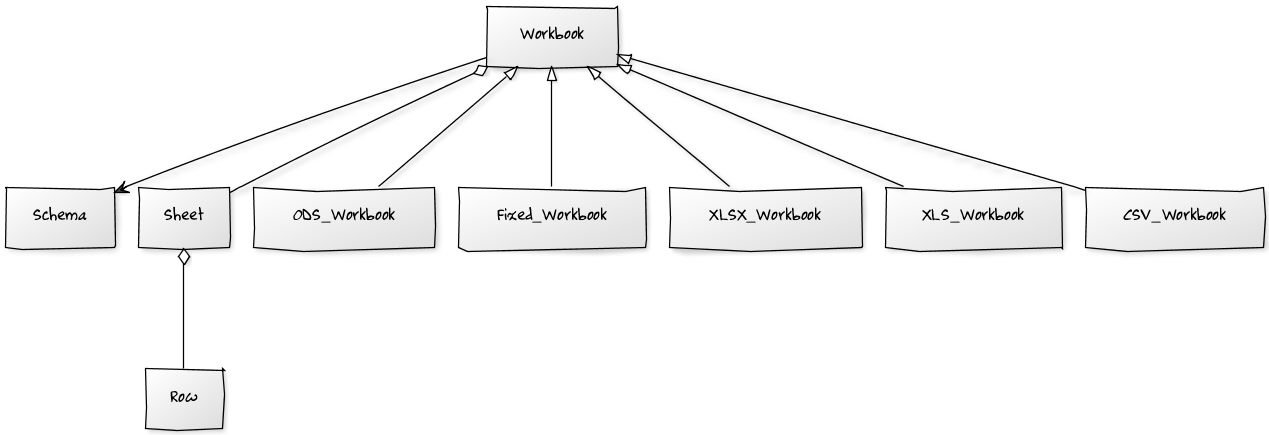
\includegraphics[width=6in]{workbook.png}


\subsection{Workbook Implementation}
\label{workbook/index:workbook-implementation}
These modules implement the various kinds of workbooks that Stingray
can process.


\subsubsection{Workbook \_\_init\_\_ Module -- Wrapper for all implementations}
\label{workbook/init:workbook-init-module-wrapper-for-all-implementations}\label{workbook/init::doc}\label{workbook/init:workbook-init}
A few Python overheads that we put in the \code{\_\_init\_\_}
module of this package. Our goal is to make it so that only
the top-level package is imported; the individual workbook modules
are not generally expected to be used by an application.
\phantomsection\label{workbook/init:module-workbook}\index{workbook (module)}
\begin{Verbatim}[commandchars=\\\{\}]
\PYG{l+s+sd}{\PYGZdq{}\PYGZdq{}\PYGZdq{}stingray.workbook \PYGZhy{}\PYGZhy{} Opens workbooks in various}
\PYG{l+s+sd}{formats, binds their associated schema, accesses them as Sheets with}
\PYG{l+s+sd}{Rows and Cells.}

\PYG{l+s+sd}{This is a kind of **Wrapper** or **Facade** that unifies :py:mod:{}`csv{}` and}
\PYG{l+s+sd}{:py:mod:{}`xlrd{}`. It handles a number of file formats including}
\PYG{l+s+sd}{:file:{}`.xlsx{}`, :file:{}`.ods{}`, and Numbers.}
\PYG{l+s+sd}{\PYGZdq{}\PYGZdq{}\PYGZdq{}}
\end{Verbatim}

In order top open files of various types, we'll bring in a number of
helpful modules.

\begin{Verbatim}[commandchars=\\\{\}]
\PYG{k+kn}{import} \PYG{n+nn}{xml.etree.cElementTree} \PYG{k+kn}{as} \PYG{n+nn}{dom}
\PYG{k+kn}{from} \PYG{n+nn}{collections} \PYG{k+kn}{import} \PYG{n}{defaultdict}
\PYG{k+kn}{import} \PYG{n+nn}{zipfile}
\PYG{k+kn}{import} \PYG{n+nn}{datetime}
\PYG{k+kn}{from} \PYG{n+nn}{io} \PYG{k+kn}{import} \PYG{n+nb}{open}
\PYG{k+kn}{import} \PYG{n+nn}{os.path}
\PYG{k+kn}{import} \PYG{n+nn}{pprint}
\PYG{k+kn}{import} \PYG{n+nn}{re}
\PYG{k+kn}{import} \PYG{n+nn}{glob}
\PYG{k+kn}{import} \PYG{n+nn}{logging}
\PYG{k+kn}{import} \PYG{n+nn}{decimal}
\end{Verbatim}

We'll rely on definitions of {\hyperref[cell:module-cell]{\code{cell}}}, {\hyperref[sheet:module-sheet]{\code{sheet}}},
and {\hyperref[schema_loader:module-schema.loader]{\code{schema.loader}}}. We have an implicit dependency on {\hyperref[schema:module-schema]{\code{schema}}}:
we'll be given schema objects to work with.

\begin{Verbatim}[commandchars=\\\{\}]
\PYG{k+kn}{import} \PYG{n+nn}{stingray.cell}
\PYG{k+kn}{import} \PYG{n+nn}{stingray.sheet}
\PYG{k+kn}{import} \PYG{n+nn}{stingray.schema.loader}
\end{Verbatim}

We'll explicitly import the top-level class definition for each
flavor of Workbook we can support. Because we import these here, these
classes will be available with a simple import of {\hyperref[workbook/init:module-workbook]{\code{workbook}}}.

\begin{Verbatim}[commandchars=\\\{\}]
\PYG{k+kn}{from} \PYG{n+nn}{stingray.workbook.csv} \PYG{k+kn}{import} \PYG{n}{CSV\PYGZus{}Workbook}
\PYG{k+kn}{from} \PYG{n+nn}{stingray.workbook.xlsx} \PYG{k+kn}{import} \PYG{n}{XLSX\PYGZus{}Workbook}
\PYG{k+kn}{from} \PYG{n+nn}{stingray.workbook.ods} \PYG{k+kn}{import} \PYG{n}{ODS\PYGZus{}Workbook}
\PYG{k+kn}{from} \PYG{n+nn}{stingray.workbook.numbers\PYGZus{}09} \PYG{k+kn}{import} \PYG{n}{Numbers09\PYGZus{}Workbook}
\PYG{k+kn}{from} \PYG{n+nn}{stingray.workbook.numbers\PYGZus{}13} \PYG{k+kn}{import} \PYG{n}{Numbers13\PYGZus{}Workbook}
\PYG{k+kn}{from} \PYG{n+nn}{stingray.workbook.fixed} \PYG{k+kn}{import} \PYG{n}{Fixed\PYGZus{}Workbook}
\end{Verbatim}


\paragraph{Exceptions}
\label{workbook/init:exceptions}\index{UnknownFormat (class in workbook)}

\begin{fulllineitems}
\phantomsection\label{workbook/init:workbook.UnknownFormat}\pysigline{\strong{class }\code{workbook.}\bfcode{UnknownFormat}}
The {\hyperref[workbook/init:workbook.UnknownFormat]{\code{UnknownFormat}}} exception is raised when a workbook can't be
opened.

\end{fulllineitems}


\begin{Verbatim}[commandchars=\\\{\}]
\PYG{k}{class} \PYG{n+nc}{UnknownFormat}\PYG{p}{(} \PYG{n+ne}{Exception} \PYG{p}{)}\PYG{p}{:}
    \PYG{l+s+sd}{\PYGZdq{}\PYGZdq{}\PYGZdq{}The workbook can\PYGZsq{}t be opened.\PYGZdq{}\PYGZdq{}\PYGZdq{}}
    \PYG{k}{pass}
\end{Verbatim}
\index{No\_Schema (class in workbook)}

\begin{fulllineitems}
\phantomsection\label{workbook/init:workbook.No_Schema}\pysigline{\strong{class }\code{workbook.}\bfcode{No\_Schema}}
The {\hyperref[workbook/init:workbook.No_Schema]{\code{No\_Schema}}} exception is raised if there's a problem
locating an external schema for a workbook.

\end{fulllineitems}


\begin{Verbatim}[commandchars=\\\{\}]
\PYG{k}{class} \PYG{n+nc}{No\PYGZus{}Schema}\PYG{p}{(} \PYG{n+ne}{Exception} \PYG{p}{)}\PYG{p}{:}
    \PYG{l+s+sd}{\PYGZdq{}\PYGZdq{}\PYGZdq{}A valid schema could not be loaded.\PYGZdq{}\PYGZdq{}\PYGZdq{}}
    \PYG{k}{pass}
\end{Verbatim}


\paragraph{Optional Modules}
\label{workbook/init:optional-modules}
The \code{workbook.package.xls} module depends on \code{xlrd}.
\href{https://pypi.python.org/pypi/xlrd/0.9.2}{https://pypi.python.org/pypi/xlrd/0.9.2} \href{http://www.lexicon.net/sjmachin/xlrd.htm}{http://www.lexicon.net/sjmachin/xlrd.htm}

We can't guarantee that \code{xlrd} is available. Also, old \code{.xls} files are
becoming less frequently used, so we're making this optional.

\begin{Verbatim}[commandchars=\\\{\}]
\PYG{k}{try}\PYG{p}{:}
    \PYG{k+kn}{from} \PYG{n+nn}{stingray.workbook.xls} \PYG{k+kn}{import} \PYG{n}{XLS\PYGZus{}Workbook}
\PYG{k}{except} \PYG{n+ne}{ImportError}\PYG{p}{:}
    \PYG{k+kn}{from} \PYG{n+nn}{stingray.workbook.base} \PYG{k+kn}{import} \PYG{n}{Workbook}
    \PYG{k}{class} \PYG{n+nc}{XLS\PYGZus{}Workbook}\PYG{p}{(} \PYG{n}{Workbook} \PYG{p}{)}\PYG{p}{:}
        \PYG{l+s+sd}{\PYGZdq{}\PYGZdq{}\PYGZdq{}No {}`{}`xlrd{}`{}` Available.\PYGZdq{}\PYGZdq{}\PYGZdq{}}
        \PYG{k}{def} \PYG{n+nf}{\PYGZus{}\PYGZus{}init\PYGZus{}\PYGZus{}}\PYG{p}{(} \PYG{n+nb+bp}{self}\PYG{p}{,} \PYG{o}{*}\PYG{n}{args}\PYG{p}{,} \PYG{o}{*}\PYG{o}{*}\PYG{n}{kw} \PYG{p}{)}\PYG{p}{:}
            \PYG{k}{raise} \PYG{n}{UnknownFormat}
\end{Verbatim}


\paragraph{Workbook Subclasses}
\label{workbook/init:workbook-subclasses}
We have a number of concrete subclasses of {\hyperref[workbook/base:workbook.base.Workbook]{\code{workbook.base.Workbook}}}.
These are imported from submodules and made visible in this module.
\begin{itemize}
\item {} 
\code{workbook.CSV\_Workbook}.  This is a degenerate case, where the workbook appears to contain
a single sheet.  This sheet is the CSV file, accessed via the built-in
\code{csv.reader()}.

\item {} 
\code{workbook.XLS\_Workbook}.  This is the workbook as processed by \code{xlrd}.  These classes
wrap \code{xlrd} classes to which the real work is delegated.
This is optional -- if \code{xlrd} is not installed, things will work,
but these files cannot be opened.

\item {} 
\code{workbook.XLSX\_Workbook}.  This is the workbook after unzipping and using an XML parser
on the various document parts.  Mostly, this is a matter of unzipping
and parsing parts of the document to create a DOM which can be traversed
as needed.

\item {} 
\code{workbook.Numbers09\_Workbook}.
This handles the iWork `09 Numbers files with multiple
workspaces and multiple tables in each workspace.

\item {} 
\code{workbook.Numbers13\_Workbook}
These handle the iWork `13 Numbers files with multiple
workspaces and multiple tables in each workspace.

\item {} 
\code{workbook.ODS\_Workbook}.

\item {} 
{\hyperref[workbook/fixed:workbook.Fixed_Workbook]{\code{workbook.Fixed\_Workbook}}}.  This is actually a fairly complex case.  The workbook will appear to
contain a single sheet; this sheet is the fixed format file.  Schema information
was required up front, unlike the other formats.

\end{itemize}

Further extensions will handle various kinds of COBOL files. They're similar to Fixed Workbooks.
See {\hyperref[cobol:cobol]{\emph{The COBOL Package}}}.

Each of these is a context manager, so we include the necessary methods.

Note that workbooks are rarely simple files.  Sometimes they are ZIP archive
members.  Sometimes, they must be processed via \textbf{gzip}. Sometimes they involve
Snappy compression.

In order to minimize the assumptions, we try to handle two forms of file processing:
\begin{itemize}
\item {} 
By name. In this case, the file name is provided. The file is opened and closed by
the Workbook using the context manager interface.

\item {} 
By file-like object. An open file-like object is provided. No additional
context management is performed. This is appropriate when a workbook is itself
a member of a larger archive.

\end{itemize}


\paragraph{Workbook Factory}
\label{workbook/init:workbook-factory}
This is the factory which creates a subclass of \code{Workbook} for a
a given file.
\index{Opener (class in workbook)}

\begin{fulllineitems}
\phantomsection\label{workbook/init:workbook.Opener}\pysigline{\strong{class }\code{workbook.}\bfcode{Opener}}
An opener \textbf{Factory} class.  A subclass can extend this to handle other file
extensions and physical formats.

\end{fulllineitems}


\begin{Verbatim}[commandchars=\\\{\}]
\PYG{k}{class} \PYG{n+nc}{Opener}\PYG{p}{:}
    \PYG{l+s+sd}{\PYGZdq{}\PYGZdq{}\PYGZdq{}An extensible opener that examines the file extension and locates}
\PYG{l+s+sd}{    a proper Workbook subclass.}
\PYG{l+s+sd}{    \PYGZdq{}\PYGZdq{}\PYGZdq{}}
    \PYG{k}{def} \PYG{n+nf}{\PYGZus{}\PYGZus{}call\PYGZus{}\PYGZus{}}\PYG{p}{(} \PYG{n+nb+bp}{self}\PYG{p}{,} \PYG{n}{name}\PYG{p}{,} \PYG{n}{file\PYGZus{}object}\PYG{o}{=}\PYG{n+nb+bp}{None}\PYG{p}{,}
        \PYG{n}{schema\PYGZus{}path}\PYG{o}{=}\PYG{l+s}{\PYGZsq{}}\PYG{l+s}{.}\PYG{l+s}{\PYGZsq{}}\PYG{p}{,} \PYG{n}{schema\PYGZus{}sheet}\PYG{o}{=} \PYG{n+nb+bp}{None}\PYG{p}{,} \PYG{o}{*}\PYG{o}{*}\PYG{n}{kw} \PYG{p}{)}\PYG{p}{:}
        \PYG{l+s+sd}{\PYGZdq{}\PYGZdq{}\PYGZdq{}Open a workbook.}

\PYG{l+s+sd}{        :param name: filename to open.}
\PYG{l+s+sd}{        :param file\PYGZus{}object: File\PYGZhy{}like object to process.  If not}
\PYG{l+s+sd}{        provided the named file will be opened.}
\PYG{l+s+sd}{        :keyword schema\PYGZus{}path: Directory with external schema files}
\PYG{l+s+sd}{        :keyword schema\PYGZus{}sheet: A sheet in an external schema workbook.}
\PYG{l+s+sd}{        \PYGZdq{}\PYGZdq{}\PYGZdq{}}
        \PYG{n}{\PYGZus{}}\PYG{p}{,} \PYG{n}{ext} \PYG{o}{=} \PYG{n}{os}\PYG{o}{.}\PYG{n}{path}\PYG{o}{.}\PYG{n}{splitext}\PYG{p}{(} \PYG{n}{name} \PYG{p}{)}
        \PYG{n}{ext} \PYG{o}{=} \PYG{n}{ext}\PYG{o}{.}\PYG{n}{lower}\PYG{p}{(}\PYG{p}{)}
        \PYG{k}{if} \PYG{n}{ext} \PYG{o}{==} \PYG{l+s}{\PYGZdq{}}\PYG{l+s}{.xls}\PYG{l+s}{\PYGZdq{}}\PYG{p}{:}
            \PYG{k}{return} \PYG{n}{XLS\PYGZus{}Workbook}\PYG{p}{(} \PYG{n}{name}\PYG{p}{,} \PYG{n}{file\PYGZus{}object} \PYG{p}{)}
        \PYG{k}{elif} \PYG{n}{ext} \PYG{o+ow}{in} \PYG{p}{(} \PYG{l+s}{\PYGZdq{}}\PYG{l+s}{.xlsx}\PYG{l+s}{\PYGZdq{}}\PYG{p}{,} \PYG{l+s}{\PYGZdq{}}\PYG{l+s}{.xlsm}\PYG{l+s}{\PYGZdq{}} \PYG{p}{)}\PYG{p}{:}
            \PYG{k}{return} \PYG{n}{XLSX\PYGZus{}Workbook}\PYG{p}{(} \PYG{n}{name}\PYG{p}{,} \PYG{n}{file\PYGZus{}object} \PYG{p}{)}
        \PYG{k}{elif} \PYG{n}{ext} \PYG{o+ow}{in} \PYG{p}{(} \PYG{l+s}{\PYGZdq{}}\PYG{l+s}{.csv}\PYG{l+s}{\PYGZdq{}}\PYG{p}{,} \PYG{p}{)}\PYG{p}{:}
            \PYG{k}{return} \PYG{n}{CSV\PYGZus{}Workbook}\PYG{p}{(} \PYG{n}{name}\PYG{p}{,} \PYG{n}{file\PYGZus{}object}\PYG{p}{,} \PYG{o}{*}\PYG{o}{*}\PYG{n}{kw} \PYG{p}{)}
        \PYG{k}{elif} \PYG{n}{ext} \PYG{o+ow}{in} \PYG{p}{(} \PYG{l+s}{\PYGZdq{}}\PYG{l+s}{.tab}\PYG{l+s}{\PYGZdq{}}\PYG{p}{,} \PYG{p}{)}\PYG{p}{:}
            \PYG{k}{return} \PYG{n}{CSV\PYGZus{}Workbook}\PYG{p}{(} \PYG{n}{name}\PYG{p}{,} \PYG{n}{file\PYGZus{}object}\PYG{p}{,} \PYG{n}{delimiter}\PYG{o}{=}\PYG{l+s}{\PYGZsq{}}\PYG{l+s+se}{\PYGZbs{}t}\PYG{l+s}{\PYGZsq{}}\PYG{p}{,} \PYG{o}{*}\PYG{o}{*}\PYG{n}{kw} \PYG{p}{)}
        \PYG{k}{elif} \PYG{n}{ext} \PYG{o+ow}{in} \PYG{p}{(} \PYG{l+s}{\PYGZdq{}}\PYG{l+s}{.ods}\PYG{l+s}{\PYGZdq{}}\PYG{p}{,} \PYG{p}{)}\PYG{p}{:}
            \PYG{k}{return} \PYG{n}{ODS\PYGZus{}Workbook}\PYG{p}{(} \PYG{n}{name}\PYG{p}{,} \PYG{n}{file\PYGZus{}object} \PYG{p}{)}
        \PYG{k}{elif} \PYG{n}{ext} \PYG{o+ow}{in} \PYG{p}{(} \PYG{l+s}{\PYGZdq{}}\PYG{l+s}{.numbers}\PYG{l+s}{\PYGZdq{}}\PYG{p}{,} \PYG{p}{)}\PYG{p}{:}
            \PYG{c}{\PYGZsh{} Directory? It\PYGZsq{}s Numbers13\PYGZus{}Workbook; Zipfile? It\PYGZsq{}s Numbers09\PYGZus{}Workbook}
            \PYG{k}{if} \PYG{n}{os}\PYG{o}{.}\PYG{n}{path}\PYG{o}{.}\PYG{n}{is\PYGZus{}dir}\PYG{p}{(} \PYG{n}{name} \PYG{p}{)}\PYG{p}{:}
                \PYG{k}{return} \PYG{n}{Numbers13\PYGZus{}Workbook}\PYG{p}{(} \PYG{n}{name}\PYG{p}{,} \PYG{n}{file\PYGZus{}object} \PYG{p}{)}
            \PYG{k}{else}\PYG{p}{:}
                \PYG{k}{return} \PYG{n}{Numbers09\PYGZus{}Workbook}\PYG{p}{(} \PYG{n}{name}\PYG{p}{,} \PYG{n}{file\PYGZus{}object} \PYG{p}{)}
        \PYG{k}{else}\PYG{p}{:}
            \PYG{c}{\PYGZsh{} Fixed format files with no specific extension}
            \PYG{c}{\PYGZsh{} Ideally :file:{}`somefile.schema{}` is the file}
            \PYG{c}{\PYGZsh{} and :file:{}`schema.csv{}` or :file:{}`schema.xlsx{}` can be tracked down.}
            \PYG{n}{schema\PYGZus{}pat}\PYG{o}{=} \PYG{n}{os}\PYG{o}{.}\PYG{n}{path}\PYG{o}{.}\PYG{n}{join}\PYG{p}{(}\PYG{n}{schema\PYGZus{}path}\PYG{p}{,} \PYG{n}{ext}\PYG{p}{[}\PYG{l+m+mi}{1}\PYG{p}{:}\PYG{p}{]}\PYG{o}{+}\PYG{l+s}{\PYGZdq{}}\PYG{l+s}{.*}\PYG{l+s}{\PYGZdq{}}\PYG{p}{)}
            \PYG{n}{schema\PYGZus{}choices}\PYG{o}{=} \PYG{n}{glob}\PYG{o}{.}\PYG{n}{glob}\PYG{p}{(} \PYG{n}{schema\PYGZus{}pat} \PYG{p}{)}
            \PYG{k}{if} \PYG{n}{schema\PYGZus{}choices}\PYG{p}{:}
                \PYG{n}{schema\PYGZus{}name}\PYG{o}{=} \PYG{n}{schema\PYGZus{}choices}\PYG{p}{[}\PYG{l+m+mi}{0}\PYG{p}{]}
                \PYG{n}{schema\PYGZus{}wb}\PYG{o}{=} \PYG{n}{open\PYGZus{}workbook}\PYG{p}{(} \PYG{n}{schema\PYGZus{}name} \PYG{p}{)}
                \PYG{n}{esl}\PYG{o}{=} \PYG{n}{stingray}\PYG{o}{.}\PYG{n}{schema}\PYG{o}{.}\PYG{n}{loader}\PYG{o}{.}\PYG{n}{ExternalSchemaLoader}\PYG{p}{(} \PYG{n}{schema\PYGZus{}wb}\PYG{p}{,} \PYG{n}{schema\PYGZus{}sheet} \PYG{p}{)}
                \PYG{n}{schema}\PYG{o}{=} \PYG{n}{esl}\PYG{o}{.}\PYG{n}{schema}\PYG{p}{(}\PYG{p}{)}
                \PYG{k}{return} \PYG{n}{Fixed\PYGZus{}Workbook}\PYG{p}{(} \PYG{n}{name}\PYG{p}{,} \PYG{n}{file\PYGZus{}object}\PYG{p}{,} \PYG{n}{schema}\PYG{o}{=}\PYG{n}{schema} \PYG{p}{)}
            \PYG{k}{else}\PYG{p}{:}
                \PYG{k}{raise} \PYG{n}{No\PYGZus{}Schema}\PYG{p}{(} \PYG{n}{schema\PYGZus{}pat} \PYG{p}{)}
\end{Verbatim}
\index{open\_workbook() (in module workbook)}

\begin{fulllineitems}
\phantomsection\label{workbook/init:workbook.open_workbook}\pysiglinewithargsret{\code{workbook.}\bfcode{open\_workbook}}{\emph{name}, \emph{file\_object}, \emph{schema\_path}, \emph{schema\_sheet}}{}
Open a workbook.

For fixed format files, we attempt to track down and load the relevant
schema file. The idea here is that a file's extension can map to the schema's
filename.

\code{somefile.\emph{schema}} would use a \code{\emph{schema}.csv} workbook as it's schema.
We'll simply try the first file that matches \code{\emph{schema}.*} to see if it's
a workbook we can open.
\begin{quote}\begin{description}
\item[{Parameters}] \leavevmode\begin{itemize}
\item {} 
\textbf{name} -- The name of the file.

\item {} 
\textbf{file\_object} -- (optional) already opened file object.

\item {} 
\textbf{schema\_path} -- (optional) filename for an external schema file.

\item {} 
\textbf{schema\_sheet} -- (optional) name of a sheet with a schema.

\end{itemize}

\end{description}\end{quote}

\end{fulllineitems}


For fixed format files, we attempt to track down and load the relevant
schema.  An application might have narrower and more specific rules
for binding file and schema.

The default {\hyperref[workbook/init:workbook.open_workbook]{\code{workbook.open\_workbook()}}} is simply an instance
of the {\hyperref[workbook/init:workbook.Opener]{\code{workbook.Opener}}}.

\begin{Verbatim}[commandchars=\\\{\}]
\PYG{n}{open\PYGZus{}workbook}\PYG{o}{=} \PYG{n}{Opener}\PYG{p}{(}\PYG{p}{)}
\end{Verbatim}

When creating a subclass, use the \textbf{Chain of Command} pattern.
This allows a user to create subclasses to handle the various other file name extensions.
Here's an example:
\begin{alltt}
class MyOpener(workbook.Opener):
    def \_\_call\_\_(self, name, file\_object=None,
        schema\_path='.', schema\_sheet=None, **kw ):
        if fnmatch(name, ``*.dat''):
            esl= stingray.schema.loader.ExternalSchemaLoader(
                os.path.join(schema\_path, ``schemafile.csv'') )
            schema= esl.schema()
            return CSV\_Workbook( name, file\_object, schema=schema, delimiter=''\textbar{}'' )
        return super().\_\_call\_\_(name, file\_object, schema\_path, schema\_sheet, **kw )
\end{alltt}

There may be application-specific rules, or command-line options that
will determine a mapping bewtween filename and physical format or filename and schema.


\subsubsection{Workbook Base Definition}
\label{workbook/base::doc}\label{workbook/base:workbook-base}\label{workbook/base:workbook-base-definition}
These are the definitions shared by all Workbook subclass definitions.

One of the common features is date conversions. Only XLS files have
peculiar date conversion issues. But we're forced to make all
spreadsheets polymorphic with respect to this anomalous behavior.
\phantomsection\label{workbook/base:module-workbook.base}\index{workbook.base (module)}
\begin{Verbatim}[commandchars=\\\{\}]
\PYG{k+kn}{import} \PYG{n+nn}{logging}
\PYG{k+kn}{import} \PYG{n+nn}{os}

\PYG{k+kn}{import} \PYG{n+nn}{stingray.sheet}
\end{Verbatim}
\index{Workbook (class in workbook.base)}

\begin{fulllineitems}
\phantomsection\label{workbook/base:workbook.base.Workbook}\pysigline{\strong{class }\code{workbook.base.}\bfcode{Workbook}}
All physical workbook formats all encode a single, common data structure.
Here are some abstract definitions.
\index{name (workbook.base.Workbook attribute)}

\begin{fulllineitems}
\phantomsection\label{workbook/base:workbook.base.Workbook.name}\pysigline{\bfcode{name}}
Filename for this workbook.

\end{fulllineitems}

\index{the\_file (workbook.base.Workbook attribute)}

\begin{fulllineitems}
\phantomsection\label{workbook/base:workbook.base.Workbook.the_file}\pysigline{\bfcode{the\_file}}
The actual open file object.

\end{fulllineitems}

\index{datemode (workbook.base.Workbook attribute)}

\begin{fulllineitems}
\phantomsection\label{workbook/base:workbook.base.Workbook.datemode}\pysigline{\bfcode{datemode}}
For XLS spreadsheets only, a datemode is required. This may not
be appropriate for all spreadsheets. It's in this superclass
for now, but may be refactored out.

\end{fulllineitems}

\index{log (workbook.base.Workbook attribute)}

\begin{fulllineitems}
\phantomsection\label{workbook/base:workbook.base.Workbook.log}\pysigline{\bfcode{log}}
Logger for Workbooks.

\end{fulllineitems}


\end{fulllineitems}


\begin{Verbatim}[commandchars=\\\{\}]
\PYG{k}{class} \PYG{n+nc}{Workbook}\PYG{p}{:}
    \PYG{l+s+sd}{\PYGZdq{}\PYGZdq{}\PYGZdq{}A workbook file; a collection of Sheets.\PYGZdq{}\PYGZdq{}\PYGZdq{}}
    \PYG{k}{def} \PYG{n+nf}{\PYGZus{}\PYGZus{}init\PYGZus{}\PYGZus{}}\PYG{p}{(} \PYG{n+nb+bp}{self}\PYG{p}{,} \PYG{n}{name}\PYG{p}{,} \PYG{n}{file\PYGZus{}object}\PYG{o}{=}\PYG{n+nb+bp}{None} \PYG{p}{)}\PYG{p}{:}
        \PYG{l+s+sd}{\PYGZdq{}\PYGZdq{}\PYGZdq{}Prepare the workbook for reading.}

\PYG{l+s+sd}{        :param name: File name}
\PYG{l+s+sd}{        :param file\PYGZus{}object: Optional file\PYGZhy{}like object.  If omitted, the named file is opened.}
\PYG{l+s+sd}{        \PYGZdq{}\PYGZdq{}\PYGZdq{}}
        \PYG{n+nb+bp}{self}\PYG{o}{.}\PYG{n}{name}\PYG{p}{,} \PYG{n+nb+bp}{self}\PYG{o}{.}\PYG{n}{file\PYGZus{}obj}\PYG{o}{=} \PYG{n}{name}\PYG{p}{,} \PYG{n}{file\PYGZus{}object}
        \PYG{n+nb+bp}{self}\PYG{o}{.}\PYG{n}{the\PYGZus{}file} \PYG{o}{=} \PYG{n+nb+bp}{None} \PYG{c}{\PYGZsh{} Any internal files}
        \PYG{n+nb+bp}{self}\PYG{o}{.}\PYG{n}{datemode}\PYG{o}{=} \PYG{l+m+mi}{0} \PYG{c}{\PYGZsh{} For xlrd}
        \PYG{n+nb+bp}{self}\PYG{o}{.}\PYG{n}{log}\PYG{o}{=} \PYG{n}{logging}\PYG{o}{.}\PYG{n}{getLogger}\PYG{p}{(} \PYG{n+nb+bp}{self}\PYG{o}{.}\PYG{n}{\PYGZus{}\PYGZus{}class\PYGZus{}\PYGZus{}}\PYG{o}{.}\PYG{n}{\PYGZus{}\PYGZus{}qualname\PYGZus{}\PYGZus{}} \PYG{p}{)}
    \PYG{k}{def} \PYG{n+nf}{\PYGZus{}\PYGZus{}repr\PYGZus{}\PYGZus{}}\PYG{p}{(} \PYG{n+nb+bp}{self} \PYG{p}{)}\PYG{p}{:}
        \PYG{k}{return} \PYG{l+s}{\PYGZdq{}}\PYG{l+s}{\PYGZob{}0\PYGZcb{}(\PYGZob{}1!r\PYGZcb{})}\PYG{l+s}{\PYGZdq{}}\PYG{o}{.}\PYG{n}{format}\PYG{p}{(} \PYG{n+nb+bp}{self}\PYG{o}{.}\PYG{n}{\PYGZus{}\PYGZus{}class\PYGZus{}\PYGZus{}}\PYG{o}{.}\PYG{n}{\PYGZus{}\PYGZus{}qualname\PYGZus{}\PYGZus{}}\PYG{p}{,} \PYG{n+nb+bp}{self}\PYG{o}{.}\PYG{n}{name} \PYG{p}{)}
\end{Verbatim}
\index{sheet() (workbook.base.Workbook method)}

\begin{fulllineitems}
\phantomsection\label{workbook/base:workbook.base.Workbook.sheet}\pysiglinewithargsret{\code{Workbook.}\bfcode{sheet}}{\emph{sheet\_name}, \emph{sheet\_type}, \emph{*args}, \emph{**kw}}{}
There are two varieties of sheets, depending on the presence or
absence of a schema.

\end{fulllineitems}


\begin{Verbatim}[commandchars=\\\{\}]
\PYG{k}{def} \PYG{n+nf}{sheet}\PYG{p}{(} \PYG{n+nb+bp}{self}\PYG{p}{,} \PYG{n}{sheet\PYGZus{}name}\PYG{p}{,} \PYG{n}{sheet\PYGZus{}type}\PYG{o}{=}\PYG{n+nb+bp}{None}\PYG{p}{,} \PYG{o}{*}\PYG{n}{args}\PYG{p}{,} \PYG{o}{*}\PYG{o}{*}\PYG{n}{kw} \PYG{p}{)}\PYG{p}{:}
    \PYG{l+s+sd}{\PYGZdq{}\PYGZdq{}\PYGZdq{}Returns a :py:class:{}`sheet.Sheet{}`, ready for processing.\PYGZdq{}\PYGZdq{}\PYGZdq{}}
    \PYG{k}{if} \PYG{n}{sheet\PYGZus{}type} \PYG{o+ow}{is} \PYG{n+nb+bp}{None}\PYG{p}{:} \PYG{n}{sheet\PYGZus{}type}\PYG{o}{=} \PYG{n}{stingray}\PYG{o}{.}\PYG{n}{sheet}\PYG{o}{.}\PYG{n}{Sheet}
    \PYG{n}{sheet} \PYG{o}{=} \PYG{n}{sheet\PYGZus{}type}\PYG{p}{(} \PYG{n+nb+bp}{self}\PYG{p}{,} \PYG{n}{sheet\PYGZus{}name}\PYG{p}{,} \PYG{o}{*}\PYG{n}{args}\PYG{p}{,} \PYG{o}{*}\PYG{o}{*}\PYG{n}{kw} \PYG{p}{)}
    \PYG{k}{return} \PYG{n}{sheet}
\end{Verbatim}
\index{sheets() (workbook.base.Workbook method)}

\begin{fulllineitems}
\phantomsection\label{workbook/base:workbook.base.Workbook.sheets}\pysiglinewithargsret{\code{Workbook.}\bfcode{sheets}}{}{}
The list of sheet names.

\end{fulllineitems}


\begin{Verbatim}[commandchars=\\\{\}]
\PYG{k}{def} \PYG{n+nf}{sheets}\PYG{p}{(} \PYG{n+nb+bp}{self} \PYG{p}{)}\PYG{p}{:}
    \PYG{l+s+sd}{\PYGZdq{}\PYGZdq{}\PYGZdq{}List of sheet names.}
\PYG{l+s+sd}{    The filename is a handy default sheet name for CSV and Fixed files.}
\PYG{l+s+sd}{    \PYGZdq{}\PYGZdq{}\PYGZdq{}}
    \PYG{n}{nm}\PYG{p}{,} \PYG{n}{\PYGZus{}} \PYG{o}{=} \PYG{n}{os}\PYG{o}{.}\PYG{n}{path}\PYG{o}{.}\PYG{n}{splitext}\PYG{p}{(} \PYG{n}{os}\PYG{o}{.}\PYG{n}{path}\PYG{o}{.}\PYG{n}{basename}\PYG{p}{(}\PYG{n+nb+bp}{self}\PYG{o}{.}\PYG{n}{name}\PYG{p}{)} \PYG{p}{)}
    \PYG{k}{return} \PYG{p}{[} \PYG{n}{nm} \PYG{p}{]}
\end{Verbatim}

The Context Manager interface.

\begin{Verbatim}[commandchars=\\\{\}]
\PYG{k}{def} \PYG{n+nf}{\PYGZus{}\PYGZus{}enter\PYGZus{}\PYGZus{}}\PYG{p}{(} \PYG{n+nb+bp}{self} \PYG{p}{)}\PYG{p}{:}
    \PYG{k}{return} \PYG{n+nb+bp}{self}
\PYG{k}{def} \PYG{n+nf}{\PYGZus{}\PYGZus{}exit\PYGZus{}\PYGZus{}}\PYG{p}{(} \PYG{n+nb+bp}{self}\PYG{p}{,} \PYG{n}{exc\PYGZus{}type}\PYG{p}{,} \PYG{n}{exc\PYGZus{}val}\PYG{p}{,} \PYG{n}{exc\PYGZus{}tb} \PYG{p}{)}\PYG{p}{:}
    \PYG{k}{if} \PYG{n+nb+bp}{self}\PYG{o}{.}\PYG{n}{the\PYGZus{}file}\PYG{p}{:}
        \PYG{n+nb+bp}{self}\PYG{o}{.}\PYG{n}{the\PYGZus{}file}\PYG{o}{.}\PYG{n}{close}\PYG{p}{(}\PYG{p}{)}
    \PYG{k}{if} \PYG{n}{exc\PYGZus{}type} \PYG{o+ow}{is} \PYG{o+ow}{not} \PYG{n+nb+bp}{None}\PYG{p}{:} \PYG{k}{return} \PYG{n+nb+bp}{False}
\end{Verbatim}
\index{rows\_of() (workbook.base.Workbook method)}

\begin{fulllineitems}
\phantomsection\label{workbook/base:workbook.base.Workbook.rows_of}\pysiglinewithargsret{\code{Workbook.}\bfcode{rows\_of}}{\emph{sheet}}{}
An iterator over rows of a given sheet.

\end{fulllineitems}


\begin{Verbatim}[commandchars=\\\{\}]
\PYG{k}{def} \PYG{n+nf}{rows\PYGZus{}of}\PYG{p}{(} \PYG{n+nb+bp}{self}\PYG{p}{,} \PYG{n}{sheet} \PYG{p}{)}\PYG{p}{:}
    \PYG{l+s+sd}{\PYGZdq{}\PYGZdq{}\PYGZdq{}An iterator over all rows of the given sheet.\PYGZdq{}\PYGZdq{}\PYGZdq{}}
    \PYG{k}{raise} \PYG{n+ne}{NotImplementedError}
\end{Verbatim}
\index{row\_get() (workbook.base.Workbook method)}

\begin{fulllineitems}
\phantomsection\label{workbook/base:workbook.base.Workbook.row_get}\pysiglinewithargsret{\code{Workbook.}\bfcode{row\_get}}{\emph{row}, \emph{attribute}}{}
Get a value from the current row using the current attribute.
This is the essential, underlying implementation to fetch data
from a row of a workbook.

\end{fulllineitems}


\begin{Verbatim}[commandchars=\\\{\}]
\PYG{k}{def} \PYG{n+nf}{row\PYGZus{}get}\PYG{p}{(} \PYG{n+nb+bp}{self}\PYG{p}{,} \PYG{n}{row}\PYG{p}{,} \PYG{n}{attribute} \PYG{p}{)}\PYG{p}{:}
    \PYG{l+s+sd}{\PYGZdq{}\PYGZdq{}\PYGZdq{}Create a Cell from the row\PYGZsq{}s data.\PYGZdq{}\PYGZdq{}\PYGZdq{}}
    \PYG{k}{raise} \PYG{n+ne}{NotImplementedError}
\end{Verbatim}

And, for proper date conversions in XLS spreadsheets only, we have
two methods. In other spreadsheets, proper system dates and times
are used in somewhat more conventional ways.


\begin{fulllineitems}
\pysigline{\bfcode{Workbook.float\_to\_date(~value~):}}
\end{fulllineitems}


\begin{Verbatim}[commandchars=\\\{\}]
\PYG{k}{def} \PYG{n+nf}{float\PYGZus{}to\PYGZus{}date}\PYG{p}{(} \PYG{n+nb+bp}{self}\PYG{p}{,} \PYG{n}{value} \PYG{p}{)}\PYG{p}{:}
    \PYG{k}{raise} \PYG{n+ne}{NotImplementedError}
\end{Verbatim}


\begin{fulllineitems}
\pysigline{\bfcode{Workbook.date\_to\_float(~value~):}}
\end{fulllineitems}


\begin{Verbatim}[commandchars=\\\{\}]
\PYG{k}{def} \PYG{n+nf}{date\PYGZus{}to\PYGZus{}float}\PYG{p}{(} \PYG{n}{value} \PYG{p}{)}\PYG{p}{:}
    \PYG{k}{raise} \PYG{n+ne}{NotImplementedError}
\end{Verbatim}

There are many distinct subclasses of {\hyperref[workbook/base:workbook.base.Workbook]{\code{workbook.base.Workbook}}}, based on the
physical file format.

Many of our physical formats don't require any physical schema information.
A \textbf{Fixed} file, however, requires
a physical format schema definition in order to decompose
each line into cells.


\subsubsection{CSV Workbook}
\label{workbook/csv:csv-workbook}\label{workbook/csv:workbook-csv}\label{workbook/csv::doc}
\begin{Verbatim}[commandchars=\\\{\}]
\PYG{k+kn}{import} \PYG{n+nn}{csv}
\PYG{k+kn}{import} \PYG{n+nn}{logging}
\PYG{k+kn}{import} \PYG{n+nn}{pprint}

\PYG{k+kn}{from} \PYG{n+nn}{stingray.workbook.base} \PYG{k+kn}{import} \PYG{n}{Workbook}
\PYG{k+kn}{import} \PYG{n+nn}{stingray.sheet}
\PYG{k+kn}{import} \PYG{n+nn}{stingray.cell}
\end{Verbatim}
\phantomsection\label{workbook/csv:module-workbook.csv}\index{workbook.csv (module)}\index{CSV\_Workbook (class in workbook.csv)}

\begin{fulllineitems}
\phantomsection\label{workbook/csv:workbook.csv.CSV_Workbook}\pysigline{\strong{class }\code{workbook.csv.}\bfcode{CSV\_Workbook}}
Extract sheets, rows and cells from a CSV file.

A wrapper for \code{csv.reader()}.  This will create proper
{\hyperref[cell:cell.TextCell]{\code{cell.TextCell}}} instances instead of the default string values
that \code{csv} normally creates.

There's only a single sheet and it matches the filename.

In addition to the superclass attributes, an additional unique
attribute is introduced here.
\index{rdr (workbook.csv.CSV\_Workbook attribute)}

\begin{fulllineitems}
\phantomsection\label{workbook/csv:workbook.csv.CSV_Workbook.rdr}\pysigline{\bfcode{rdr}}
The csv reader for this file.

\end{fulllineitems}


\end{fulllineitems}


\begin{Verbatim}[commandchars=\\\{\}]
\PYG{k}{class} \PYG{n+nc}{CSV\PYGZus{}Workbook}\PYG{p}{(} \PYG{n}{Workbook} \PYG{p}{)}\PYG{p}{:}
    \PYG{l+s+sd}{\PYGZdq{}\PYGZdq{}\PYGZdq{}Uses {}`{}`csv.reader{}`{}`.  There\PYGZsq{}s one sheet only.\PYGZdq{}\PYGZdq{}\PYGZdq{}}
    \PYG{k}{def} \PYG{n+nf}{\PYGZus{}\PYGZus{}init\PYGZus{}\PYGZus{}}\PYG{p}{(} \PYG{n+nb+bp}{self}\PYG{p}{,} \PYG{n}{name}\PYG{p}{,} \PYG{n}{file\PYGZus{}object}\PYG{o}{=}\PYG{n+nb+bp}{None}\PYG{p}{,} \PYG{o}{*}\PYG{o}{*}\PYG{n}{kw} \PYG{p}{)}\PYG{p}{:}
        \PYG{l+s+sd}{\PYGZdq{}\PYGZdq{}\PYGZdq{}Prepare the workbook for reading.}
\PYG{l+s+sd}{        :param name: File name}
\PYG{l+s+sd}{        :param file\PYGZus{}object: Optional file\PYGZhy{}like object.  If omitted, the named file is opened.}
\PYG{l+s+sd}{            If provided, it must be opened with  newline=\PYGZsq{}\PYGZsq{} to permit non\PYGZhy{}standard}
\PYG{l+s+sd}{            line\PYGZhy{}endings.}

\PYG{l+s+sd}{        The kw are passed to :py:func:{}`csv.reader{}`}
\PYG{l+s+sd}{        to provide dialect information.\PYGZdq{}\PYGZdq{}\PYGZdq{}}
        \PYG{n+nb}{super}\PYG{p}{(}\PYG{p}{)}\PYG{o}{.}\PYG{n}{\PYGZus{}\PYGZus{}init\PYGZus{}\PYGZus{}}\PYG{p}{(} \PYG{n}{name}\PYG{p}{,} \PYG{n}{file\PYGZus{}object} \PYG{p}{)}
        \PYG{k}{if} \PYG{n+nb+bp}{self}\PYG{o}{.}\PYG{n}{file\PYGZus{}obj}\PYG{p}{:}
            \PYG{n+nb+bp}{self}\PYG{o}{.}\PYG{n}{the\PYGZus{}file}\PYG{o}{=} \PYG{n+nb+bp}{None}
            \PYG{n+nb+bp}{self}\PYG{o}{.}\PYG{n}{rdr}\PYG{o}{=} \PYG{n}{csv}\PYG{o}{.}\PYG{n}{reader}\PYG{p}{(} \PYG{n+nb+bp}{self}\PYG{o}{.}\PYG{n}{file\PYGZus{}obj}\PYG{p}{,} \PYG{o}{*}\PYG{o}{*}\PYG{n}{kw} \PYG{p}{)}
        \PYG{k}{else}\PYG{p}{:}
            \PYG{n+nb+bp}{self}\PYG{o}{.}\PYG{n}{the\PYGZus{}file} \PYG{o}{=} \PYG{n+nb}{open}\PYG{p}{(} \PYG{n}{name}\PYG{p}{,} \PYG{l+s}{\PYGZsq{}}\PYG{l+s}{r}\PYG{l+s}{\PYGZsq{}}\PYG{p}{,} \PYG{n}{newline}\PYG{o}{=}\PYG{l+s}{\PYGZsq{}}\PYG{l+s}{\PYGZsq{}} \PYG{p}{)}
            \PYG{n+nb+bp}{self}\PYG{o}{.}\PYG{n}{rdr}\PYG{o}{=} \PYG{n}{csv}\PYG{o}{.}\PYG{n}{reader}\PYG{p}{(} \PYG{n+nb+bp}{self}\PYG{o}{.}\PYG{n}{the\PYGZus{}file}\PYG{p}{,} \PYG{o}{*}\PYG{o}{*}\PYG{n}{kw} \PYG{p}{)}
\end{Verbatim}

We can build an eager {\hyperref[sheet:sheet.Row]{\code{sheet.Row}}} or a {\hyperref[sheet:sheet.LazyRow]{\code{sheet.LazyRow}}} from
the available data.
The eager Row includes the conversions.  The {\hyperref[sheet:sheet.LazyRow]{\code{sheet.LazyRow}}} defers
the conversions until the callback to {\hyperref[workbook/base:workbook.base.Workbook.row_get]{\code{workbook.base.Workbook.row\_get()}}}.
\index{rows\_of() (workbook.csv.CSV\_Workbook method)}

\begin{fulllineitems}
\phantomsection\label{workbook/csv:workbook.csv.CSV_Workbook.rows_of}\pysiglinewithargsret{\code{CSV\_Workbook.}\bfcode{rows\_of}}{\emph{sheet}}{}
Iterator through all rows. The sheet is ignored.

\end{fulllineitems}


\begin{Verbatim}[commandchars=\\\{\}]
\PYG{k}{def} \PYG{n+nf}{rows\PYGZus{}of}\PYG{p}{(} \PYG{n+nb+bp}{self}\PYG{p}{,} \PYG{n}{sheet} \PYG{p}{)}\PYG{p}{:}
    \PYG{l+s+sd}{\PYGZdq{}\PYGZdq{}\PYGZdq{}An iterator over all rows of the named sheet.}
\PYG{l+s+sd}{    For CSV files, the sheet.name is simply ignored.}
\PYG{l+s+sd}{    \PYGZdq{}\PYGZdq{}\PYGZdq{}}
    \PYG{k}{for} \PYG{n}{data} \PYG{o+ow}{in} \PYG{n+nb+bp}{self}\PYG{o}{.}\PYG{n}{rdr}\PYG{p}{:}
        \PYG{n}{logging}\PYG{o}{.}\PYG{n}{debug}\PYG{p}{(} \PYG{n}{pprint}\PYG{o}{.}\PYG{n}{pformat}\PYG{p}{(} \PYG{n}{data}\PYG{p}{,} \PYG{n}{indent}\PYG{o}{=}\PYG{l+m+mi}{4} \PYG{p}{)} \PYG{p}{)}
        \PYG{n}{row} \PYG{o}{=} \PYG{n}{stingray}\PYG{o}{.}\PYG{n}{sheet}\PYG{o}{.}\PYG{n}{Row}\PYG{p}{(} \PYG{n}{sheet}\PYG{p}{,} \PYG{o}{*}\PYG{p}{(}\PYG{n}{stingray}\PYG{o}{.}\PYG{n}{cell}\PYG{o}{.}\PYG{n}{TextCell}\PYG{p}{(}\PYG{n}{col}\PYG{p}{,}\PYG{n+nb+bp}{self}\PYG{p}{)} \PYG{k}{for} \PYG{n}{col} \PYG{o+ow}{in} \PYG{n}{data}\PYG{p}{)} \PYG{p}{)}
        \PYG{k}{yield} \PYG{n}{row}
\end{Verbatim}
\index{row\_get() (workbook.csv.CSV\_Workbook method)}

\begin{fulllineitems}
\phantomsection\label{workbook/csv:workbook.csv.CSV_Workbook.row_get}\pysiglinewithargsret{\code{CSV\_Workbook.}\bfcode{row\_get}}{\emph{row}, \emph{attribute}}{}
Concrete implementation to get an attribute's value from a given row.

\end{fulllineitems}


\begin{Verbatim}[commandchars=\\\{\}]
\PYG{k}{def} \PYG{n+nf}{row\PYGZus{}get}\PYG{p}{(} \PYG{n+nb+bp}{self}\PYG{p}{,} \PYG{n}{row}\PYG{p}{,} \PYG{n}{attribute} \PYG{p}{)}\PYG{p}{:}
    \PYG{l+s+sd}{\PYGZdq{}\PYGZdq{}\PYGZdq{}Create a Cell from the row\PYGZsq{}s data.\PYGZdq{}\PYGZdq{}\PYGZdq{}}
    \PYG{k}{return} \PYG{n}{row}\PYG{p}{[}\PYG{n}{attribute}\PYG{o}{.}\PYG{n}{position}\PYG{p}{]}
\end{Verbatim}

Since \code{csv} is eager, returning an individual {\hyperref[cell:cell.TextCell]{\code{cell.TextCell}}}
is easy.


\subsubsection{XLS Workbook}
\label{workbook/xls:xls-workbook}\label{workbook/xls::doc}\label{workbook/xls:workbook-xls}
\begin{Verbatim}[commandchars=\\\{\}]
\PYG{k+kn}{import} \PYG{n+nn}{logging}
\PYG{k+kn}{import} \PYG{n+nn}{pprint}

\PYG{k+kn}{from} \PYG{n+nn}{stingray.workbook.base} \PYG{k+kn}{import} \PYG{n}{Workbook}
\PYG{k+kn}{import} \PYG{n+nn}{stingray.sheet}
\PYG{k+kn}{import} \PYG{n+nn}{stingray.cell}

\PYG{k+kn}{import} \PYG{n+nn}{xlrd}
\end{Verbatim}
\phantomsection\label{workbook/xls:module-workbook.xls}\index{workbook.xls (module)}\index{XLS\_Workbook (class in workbook.xls)}

\begin{fulllineitems}
\phantomsection\label{workbook/xls:workbook.xls.XLS_Workbook}\pysigline{\strong{class }\code{workbook.xls.}\bfcode{XLS\_Workbook}}
Extract sheets, rows and cells from an XLS format file.

This definition of a workbook wraps \code{xlrd} so that it fits the Stingray framework.
We'll use proper {\hyperref[cell:cell.Cell]{\code{cell.Cell}}} subclass instances instead of the default \code{xlrd.Cell}
values that \code{xlrd} normally creates.

In addition to the superclass attributes, some additional unique
attributes are introduced here.
\index{wb (workbook.xls.XLS\_Workbook attribute)}

\begin{fulllineitems}
\phantomsection\label{workbook/xls:workbook.xls.XLS_Workbook.wb}\pysigline{\bfcode{wb}}
A xlrd workbook for this file.

\end{fulllineitems}

\index{datemode (workbook.xls.XLS\_Workbook attribute)}

\begin{fulllineitems}
\phantomsection\label{workbook/xls:workbook.xls.XLS_Workbook.datemode}\pysigline{\bfcode{datemode}}
The XLS date mode for this workbook. This is required for converting
floating-point values to dates and dates to floating-point values.

\end{fulllineitems}


\end{fulllineitems}


\begin{Verbatim}[commandchars=\\\{\}]
\PYG{k}{class} \PYG{n+nc}{XLS\PYGZus{}Workbook}\PYG{p}{(} \PYG{n}{Workbook} \PYG{p}{)}\PYG{p}{:}
    \PYG{l+s+sd}{\PYGZdq{}\PYGZdq{}\PYGZdq{}Uses {}`{}`xlrd{}`{}`.\PYGZdq{}\PYGZdq{}\PYGZdq{}}
    \PYG{k}{def} \PYG{n+nf}{\PYGZus{}\PYGZus{}init\PYGZus{}\PYGZus{}}\PYG{p}{(} \PYG{n+nb+bp}{self}\PYG{p}{,} \PYG{n}{name}\PYG{p}{,} \PYG{n}{file\PYGZus{}object}\PYG{o}{=}\PYG{n+nb+bp}{None}\PYG{p}{,} \PYG{o}{*}\PYG{o}{*}\PYG{n}{kw} \PYG{p}{)}\PYG{p}{:}
        \PYG{l+s+sd}{\PYGZdq{}\PYGZdq{}\PYGZdq{}Prepare the workbook for reading.}
\PYG{l+s+sd}{        :param name: File name}
\PYG{l+s+sd}{        :param file\PYGZus{}object: Optional file\PYGZhy{}like object.  If omitted, the named file is opened.}

\PYG{l+s+sd}{        The kw arguments are passed to :py:func:{}`xlrd.open\PYGZus{}workbook{}`.}
\PYG{l+s+sd}{        \PYGZdq{}\PYGZdq{}\PYGZdq{}}
        \PYG{n+nb}{super}\PYG{p}{(}\PYG{p}{)}\PYG{o}{.}\PYG{n}{\PYGZus{}\PYGZus{}init\PYGZus{}\PYGZus{}}\PYG{p}{(} \PYG{n}{name}\PYG{p}{,} \PYG{n}{file\PYGZus{}object} \PYG{p}{)}
        \PYG{k}{if} \PYG{n+nb+bp}{self}\PYG{o}{.}\PYG{n}{file\PYGZus{}obj}\PYG{p}{:}
            \PYG{n+nb+bp}{self}\PYG{o}{.}\PYG{n}{wb}\PYG{o}{=} \PYG{n}{xlrd}\PYG{o}{.}\PYG{n}{open\PYGZus{}workbook}\PYG{p}{(} \PYG{n+nb+bp}{self}\PYG{o}{.}\PYG{n}{name}\PYG{p}{,} \PYG{n}{file\PYGZus{}contents}\PYG{o}{=}\PYG{n+nb+bp}{self}\PYG{o}{.}\PYG{n}{file\PYGZus{}obj}\PYG{o}{.}\PYG{n}{read}\PYG{p}{(}\PYG{p}{)}\PYG{p}{,} \PYG{o}{*}\PYG{o}{*}\PYG{n}{kw} \PYG{p}{)}
        \PYG{k}{else}\PYG{p}{:}
            \PYG{n+nb+bp}{self}\PYG{o}{.}\PYG{n}{wb}\PYG{o}{=} \PYG{n}{xlrd}\PYG{o}{.}\PYG{n}{open\PYGZus{}workbook}\PYG{p}{(} \PYG{n+nb+bp}{self}\PYG{o}{.}\PYG{n}{name}\PYG{p}{,} \PYG{o}{*}\PYG{o}{*}\PYG{n}{kw} \PYG{p}{)}
        \PYG{n+nb+bp}{self}\PYG{o}{.}\PYG{n}{datemode}\PYG{o}{=} \PYG{n+nb+bp}{self}\PYG{o}{.}\PYG{n}{wb}\PYG{o}{.}\PYG{n}{datemode}
\end{Verbatim}
\index{sheets() (workbook.xls.XLS\_Workbook method)}

\begin{fulllineitems}
\phantomsection\label{workbook/xls:workbook.xls.XLS_Workbook.sheets}\pysiglinewithargsret{\code{XLS\_Workbook.}\bfcode{sheets}}{}{}
Return the list of sheets for this workbook.

\end{fulllineitems}


\begin{Verbatim}[commandchars=\\\{\}]
\PYG{k}{def} \PYG{n+nf}{sheets}\PYG{p}{(} \PYG{n+nb+bp}{self} \PYG{p}{)}\PYG{p}{:}
    \PYG{l+s+sd}{\PYGZdq{}\PYGZdq{}\PYGZdq{}List of sheet names.\PYGZdq{}\PYGZdq{}\PYGZdq{}}
    \PYG{k}{return} \PYG{n+nb+bp}{self}\PYG{o}{.}\PYG{n}{wb}\PYG{o}{.}\PYG{n}{sheet\PYGZus{}names}\PYG{p}{(}\PYG{p}{)}
\end{Verbatim}

We can build an eager {\hyperref[sheet:sheet.Row]{\code{sheet.Row}}} or a {\hyperref[sheet:sheet.LazyRow]{\code{sheet.LazyRow}}} from the available data.
The eager Row includes the conversions.  The LazyRow defers the conversions
until the callback to {\hyperref[workbook/xls:workbook.xls.XLS_Workbook.row_get]{\code{XLS\_Workbook.row\_get()}}}.
\index{rows\_of() (workbook.xls.XLS\_Workbook method)}

\begin{fulllineitems}
\phantomsection\label{workbook/xls:workbook.xls.XLS_Workbook.rows_of}\pysiglinewithargsret{\code{XLS\_Workbook.}\bfcode{rows\_of}}{\emph{sheet}}{}
Iterate through rows of the given sheet.

\end{fulllineitems}


\begin{Verbatim}[commandchars=\\\{\}]
\PYG{k}{def} \PYG{n+nf}{rows\PYGZus{}of}\PYG{p}{(} \PYG{n+nb+bp}{self}\PYG{p}{,} \PYG{n}{sheet} \PYG{p}{)}\PYG{p}{:}
    \PYG{l+s+sd}{\PYGZdq{}\PYGZdq{}\PYGZdq{}An iterator over all rows of the given sheet.\PYGZdq{}\PYGZdq{}\PYGZdq{}}
    \PYG{n+nb+bp}{self}\PYG{o}{.}\PYG{n}{sheet}\PYG{o}{=} \PYG{n+nb+bp}{self}\PYG{o}{.}\PYG{n}{wb}\PYG{o}{.}\PYG{n}{sheet\PYGZus{}by\PYGZus{}name}\PYG{p}{(}\PYG{n}{sheet}\PYG{o}{.}\PYG{n}{name}\PYG{p}{)}
    \PYG{k}{for} \PYG{n}{n} \PYG{o+ow}{in} \PYG{n+nb}{range}\PYG{p}{(}\PYG{n+nb+bp}{self}\PYG{o}{.}\PYG{n}{sheet}\PYG{o}{.}\PYG{n}{nrows}\PYG{p}{)}\PYG{p}{:}
        \PYG{n}{data} \PYG{o}{=} \PYG{n+nb+bp}{self}\PYG{o}{.}\PYG{n}{sheet}\PYG{o}{.}\PYG{n}{row}\PYG{p}{(}\PYG{n}{n}\PYG{p}{)}
        \PYG{n}{row} \PYG{o}{=} \PYG{n}{stingray}\PYG{o}{.}\PYG{n}{sheet}\PYG{o}{.}\PYG{n}{Row}\PYG{p}{(} \PYG{n}{sheet}\PYG{p}{,} \PYG{o}{*}\PYG{p}{(}\PYG{n+nb+bp}{self}\PYG{o}{.}\PYG{n}{cell}\PYG{p}{(}\PYG{n}{col}\PYG{p}{)} \PYG{k}{for} \PYG{n}{col} \PYG{o+ow}{in} \PYG{n}{data}\PYG{p}{)} \PYG{p}{)}
        \PYG{k}{yield} \PYG{n}{row}
\end{Verbatim}
\index{row\_get() (workbook.xls.XLS\_Workbook method)}

\begin{fulllineitems}
\phantomsection\label{workbook/xls:workbook.xls.XLS_Workbook.row_get}\pysiglinewithargsret{\code{XLS\_Workbook.}\bfcode{row\_get}}{\emph{row}, \emph{attribute}}{}
Low-level get of a particular attribute from the given row.

\end{fulllineitems}


\begin{Verbatim}[commandchars=\\\{\}]
\PYG{k}{def} \PYG{n+nf}{row\PYGZus{}get}\PYG{p}{(} \PYG{n+nb+bp}{self}\PYG{p}{,} \PYG{n}{row}\PYG{p}{,} \PYG{n}{attribute} \PYG{p}{)}\PYG{p}{:}
    \PYG{l+s+sd}{\PYGZdq{}\PYGZdq{}\PYGZdq{}Create a Cell from the row\PYGZsq{}s data.\PYGZdq{}\PYGZdq{}\PYGZdq{}}
    \PYG{k}{return} \PYG{n}{row}\PYG{p}{[}\PYG{n}{attribute}\PYG{o}{.}\PYG{n}{position}\PYG{p}{]}
\end{Verbatim}
\index{cell() (workbook.xls.XLS\_Workbook method)}

\begin{fulllineitems}
\phantomsection\label{workbook/xls:workbook.xls.XLS_Workbook.cell}\pysiglinewithargsret{\code{XLS\_Workbook.}\bfcode{cell}}{\emph{row}, \emph{xlrd\_cell}}{}
In {\hyperref[workbook/xls:workbook.xls.XLS_Workbook.rows_of]{\code{XLS\_Workbook.rows\_of()}}} we built a row eagerly.
That way, returning an individual Cell is easy.

Convert a single \code{xlrd.Cell} to a proper subclass of {\hyperref[cell:cell.Cell]{\code{cell.Cell}}}

\end{fulllineitems}


\begin{Verbatim}[commandchars=\\\{\}]
\PYG{k}{def} \PYG{n+nf}{cell}\PYG{p}{(} \PYG{n+nb+bp}{self}\PYG{p}{,} \PYG{n}{xlrd\PYGZus{}cell} \PYG{p}{)}\PYG{p}{:}
    \PYG{k}{if} \PYG{n}{xlrd\PYGZus{}cell}\PYG{o}{.}\PYG{n}{ctype} \PYG{o}{==} \PYG{n}{xlrd}\PYG{o}{.}\PYG{n}{XL\PYGZus{}CELL\PYGZus{}EMPTY}\PYG{p}{:}
        \PYG{k}{return} \PYG{n}{stingray}\PYG{o}{.}\PYG{n}{cell}\PYG{o}{.}\PYG{n}{EmptyCell}\PYG{p}{(}\PYG{l+s}{\PYGZsq{}}\PYG{l+s}{\PYGZsq{}}\PYG{p}{,} \PYG{n+nb+bp}{self}\PYG{p}{)}
    \PYG{k}{elif} \PYG{n}{xlrd\PYGZus{}cell}\PYG{o}{.}\PYG{n}{ctype} \PYG{o}{==} \PYG{n}{xlrd}\PYG{o}{.}\PYG{n}{XL\PYGZus{}CELL\PYGZus{}TEXT}\PYG{p}{:}
        \PYG{k}{return} \PYG{n}{stingray}\PYG{o}{.}\PYG{n}{cell}\PYG{o}{.}\PYG{n}{TextCell}\PYG{p}{(} \PYG{n}{xlrd\PYGZus{}cell}\PYG{o}{.}\PYG{n}{value}\PYG{p}{,} \PYG{n+nb+bp}{self} \PYG{p}{)}
    \PYG{k}{elif} \PYG{n}{xlrd\PYGZus{}cell}\PYG{o}{.}\PYG{n}{ctype} \PYG{o}{==} \PYG{n}{xlrd}\PYG{o}{.}\PYG{n}{XL\PYGZus{}CELL\PYGZus{}NUMBER}\PYG{p}{:}
        \PYG{k}{return} \PYG{n}{stingray}\PYG{o}{.}\PYG{n}{cell}\PYG{o}{.}\PYG{n}{NumberCell}\PYG{p}{(} \PYG{n}{xlrd\PYGZus{}cell}\PYG{o}{.}\PYG{n}{value}\PYG{p}{,} \PYG{n+nb+bp}{self} \PYG{p}{)}
    \PYG{k}{elif} \PYG{n}{xlrd\PYGZus{}cell}\PYG{o}{.}\PYG{n}{ctype} \PYG{o}{==} \PYG{n}{xlrd}\PYG{o}{.}\PYG{n}{XL\PYGZus{}CELL\PYGZus{}DATE}\PYG{p}{:}
        \PYG{k}{return} \PYG{n}{stingray}\PYG{o}{.}\PYG{n}{cell}\PYG{o}{.}\PYG{n}{FloatDateCell}\PYG{p}{(} \PYG{n}{xlrd\PYGZus{}cell}\PYG{o}{.}\PYG{n}{value}\PYG{p}{,} \PYG{n+nb+bp}{self} \PYG{p}{)}
    \PYG{k}{elif} \PYG{n}{xlrd\PYGZus{}cell}\PYG{o}{.}\PYG{n}{ctype} \PYG{o}{==} \PYG{n}{xlrd}\PYG{o}{.}\PYG{n}{XL\PYGZus{}CELL\PYGZus{}BOOLEAN}\PYG{p}{:}
        \PYG{k}{return} \PYG{n}{stingray}\PYG{o}{.}\PYG{n}{cell}\PYG{o}{.}\PYG{n}{BooleanCell}\PYG{p}{(} \PYG{n}{xlrd\PYGZus{}cell}\PYG{o}{.}\PYG{n}{value}\PYG{p}{,} \PYG{n+nb+bp}{self} \PYG{p}{)}
    \PYG{k}{elif} \PYG{n}{xlrd\PYGZus{}cell}\PYG{o}{.}\PYG{n}{ctype} \PYG{o}{==} \PYG{n}{xlrd}\PYG{o}{.}\PYG{n}{XL\PYGZus{}CELL\PYGZus{}ERROR}\PYG{p}{:}
        \PYG{k}{return} \PYG{n}{stingray}\PYG{o}{.}\PYG{n}{cell}\PYG{o}{.}\PYG{n}{ErrorCell}\PYG{p}{(}
            \PYG{n}{xlrd}\PYG{o}{.}\PYG{n}{error\PYGZus{}text\PYGZus{}from\PYGZus{}code}\PYG{p}{[}\PYG{n}{xlrd\PYGZus{}cell}\PYG{o}{.}\PYG{n}{value}\PYG{p}{]}\PYG{p}{,} \PYG{n+nb+bp}{self} \PYG{p}{)}
    \PYG{k}{elif} \PYG{n}{xlrd\PYGZus{}cell}\PYG{o}{.}\PYG{n}{ctype} \PYG{o}{==} \PYG{n}{xlrd}\PYG{o}{.}\PYG{n}{XL\PYGZus{}CELL\PYGZus{}BLANK}\PYG{p}{:}
        \PYG{k}{return} \PYG{n}{stingray}\PYG{o}{.}\PYG{n}{cell}\PYG{o}{.}\PYG{n}{EmptyCell}\PYG{p}{(}\PYG{l+s}{\PYGZsq{}}\PYG{l+s}{\PYGZsq{}}\PYG{p}{,} \PYG{n+nb+bp}{self}\PYG{p}{)}
    \PYG{k}{else}\PYG{p}{:}
        \PYG{k}{raise} \PYG{n+ne}{ValueError}\PYG{p}{(} \PYG{l+s}{\PYGZdq{}}\PYG{l+s}{Damaged Workbook}\PYG{l+s}{\PYGZdq{}} \PYG{p}{)}
\end{Verbatim}

For proper date conversions, we have
two methods that leverage the datemode to properly convert dates
and times in \code{.XLS} workbooks.


\begin{fulllineitems}
\pysigline{\bfcode{Workbook.float\_to\_date(~value~):}}
\end{fulllineitems}


\begin{Verbatim}[commandchars=\\\{\}]
\PYG{k}{def} \PYG{n+nf}{float\PYGZus{}to\PYGZus{}date}\PYG{p}{(} \PYG{n+nb+bp}{self}\PYG{p}{,} \PYG{n}{value} \PYG{p}{)}\PYG{p}{:}
    \PYG{k}{try}\PYG{p}{:}
        \PYG{n}{dt}\PYG{o}{=} \PYG{n}{xlrd}\PYG{o}{.}\PYG{n}{xldate\PYGZus{}as\PYGZus{}tuple}\PYG{p}{(}\PYG{n}{value}\PYG{p}{,} \PYG{n+nb+bp}{self}\PYG{o}{.}\PYG{n}{datemode}\PYG{p}{)}
    \PYG{k}{except} \PYG{n}{xlrd}\PYG{o}{.}\PYG{n}{xldate}\PYG{o}{.}\PYG{n}{XLDateAmbiguous} \PYG{k}{as} \PYG{n}{e}\PYG{p}{:}
        \PYG{n}{ex}\PYG{o}{=} \PYG{n+ne}{ValueError}\PYG{p}{(} \PYG{l+s}{\PYGZdq{}}\PYG{l+s}{Ambiguous Date: \PYGZob{}0!r\PYGZcb{}}\PYG{l+s}{\PYGZdq{}}\PYG{o}{.}\PYG{n}{format}\PYG{p}{(}\PYG{n}{value}\PYG{p}{)} \PYG{p}{)}
        \PYG{k}{raise} \PYG{n}{ex} \PYG{k+kn}{from} \PYG{n+nn}{e}
    \PYG{k}{return} \PYG{n}{datetime}\PYG{o}{.}\PYG{n}{datetime}\PYG{p}{(}\PYG{o}{*}\PYG{n}{dt}\PYG{p}{)}
\end{Verbatim}


\begin{fulllineitems}
\pysigline{\bfcode{Workbook.date\_to\_float(~value~):}}
\end{fulllineitems}


\begin{Verbatim}[commandchars=\\\{\}]
\PYG{k}{def} \PYG{n+nf}{date\PYGZus{}to\PYGZus{}float}\PYG{p}{(} \PYG{n}{value} \PYG{p}{)}\PYG{p}{:}
    \PYG{n}{timetuple}\PYG{o}{=} \PYG{n+nb+bp}{self}\PYG{o}{.}\PYG{n}{value}\PYG{o}{.}\PYG{n}{timetuple}\PYG{p}{(}\PYG{p}{)}\PYG{p}{[}\PYG{p}{:}\PYG{l+m+mi}{6}\PYG{p}{]}
    \PYG{n}{xl}\PYG{o}{=} \PYG{n}{xlrd}\PYG{o}{.}\PYG{n}{xldate}\PYG{o}{.}\PYG{n}{xldate\PYGZus{}from\PYGZus{}datetime\PYGZus{}tuple}\PYG{p}{(}
        \PYG{n}{timetuple}\PYG{p}{,}
        \PYG{n+nb+bp}{self}\PYG{o}{.}\PYG{n}{datemode}\PYG{p}{)}
    \PYG{k}{return} \PYG{n}{xl}
\end{Verbatim}


\subsubsection{XLSX or XLSM Workbook}
\label{workbook/xlsx:workbook-xlsx}\label{workbook/xlsx:xlsx-or-xlsm-workbook}\label{workbook/xlsx::doc}
\begin{Verbatim}[commandchars=\\\{\}]
\PYG{k+kn}{import} \PYG{n+nn}{logging}
\PYG{k+kn}{import} \PYG{n+nn}{pprint}
\PYG{k+kn}{import} \PYG{n+nn}{xml.etree.cElementTree} \PYG{k+kn}{as} \PYG{n+nn}{dom}
\PYG{k+kn}{import} \PYG{n+nn}{re}
\PYG{k+kn}{import} \PYG{n+nn}{zipfile}
\PYG{k+kn}{from} \PYG{n+nn}{collections} \PYG{k+kn}{import} \PYG{n}{defaultdict}

\PYG{k+kn}{from} \PYG{n+nn}{stingray.workbook.base} \PYG{k+kn}{import} \PYG{n}{Workbook}
\PYG{k+kn}{import} \PYG{n+nn}{stingray.sheet}
\PYG{k+kn}{import} \PYG{n+nn}{stingray.cell}
\end{Verbatim}
\phantomsection\label{workbook/xlsx:module-workbook.xlsx}\index{workbook.xlsx (module)}\index{XLSX\_Workbook (class in workbook.xlsx)}

\begin{fulllineitems}
\phantomsection\label{workbook/xlsx:workbook.xlsx.XLSX_Workbook}\pysigline{\strong{class }\code{workbook.xlsx.}\bfcode{XLSX\_Workbook}}
Extract sheets, rows and cells from an XLSX format file.

We're opening a ZIP archive and parsing the various XML documents
that we find therein.

The \code{ElementTree} incremental parser provides
parse ``events'' for specific tags, allowing for lower-memory parsing of
the sometimes large XML documents.

See \href{http://effbot.org/zone/element-iterparse.htm}{http://effbot.org/zone/element-iterparse.htm}

The class as a whole defines some handy constants like XML namespaces
and a pattern for parsing Cell ID's to separate the letters from the numbers.

In addition to the superclass attributes, some additional unique
attributes are introduced here.
\index{zip\_archive (workbook.xlsx.XLSX\_Workbook attribute)}

\begin{fulllineitems}
\phantomsection\label{workbook/xlsx:workbook.xlsx.XLSX_Workbook.zip_archive}\pysigline{\bfcode{zip\_archive}}
A zip archive for this file.

\end{fulllineitems}

\index{strings\_dict (workbook.xlsx.XLSX\_Workbook attribute)}

\begin{fulllineitems}
\phantomsection\label{workbook/xlsx:workbook.xlsx.XLSX_Workbook.strings_dict}\pysigline{\bfcode{strings\_dict}}
The strings in this workbook

\end{fulllineitems}


\end{fulllineitems}


\begin{Verbatim}[commandchars=\\\{\}]
\PYG{k}{class} \PYG{n+nc}{XLSX\PYGZus{}Workbook}\PYG{p}{(} \PYG{n}{Workbook} \PYG{p}{)}\PYG{p}{:}
    \PYG{l+s+sd}{\PYGZdq{}\PYGZdq{}\PYGZdq{}ECMA Standard XLSX or XLSM documents.}
\PYG{l+s+sd}{    Locate sheets and rows within a given sheet.}

\PYG{l+s+sd}{    See http://www.ecma\PYGZhy{}international.org/publications/standards/Ecma\PYGZhy{}376.htm}
\PYG{l+s+sd}{    \PYGZdq{}\PYGZdq{}\PYGZdq{}}
    \PYG{c}{\PYGZsh{} Relevant subset of namespaces used}
    \PYG{n}{XLSX\PYGZus{}NS} \PYG{o}{=} \PYG{p}{\PYGZob{}}
    \PYG{l+s}{\PYGZdq{}}\PYG{l+s}{main}\PYG{l+s}{\PYGZdq{}}\PYG{p}{:}\PYG{l+s}{\PYGZdq{}}\PYG{l+s}{http://schemas.openxmlformats.org/spreadsheetml/2006/main}\PYG{l+s}{\PYGZdq{}}\PYG{p}{,}
    \PYG{l+s}{\PYGZdq{}}\PYG{l+s}{r}\PYG{l+s}{\PYGZdq{}}\PYG{p}{:}\PYG{l+s}{\PYGZdq{}}\PYG{l+s}{http://schemas.openxmlformats.org/officeDocument/2006/relationships}\PYG{l+s}{\PYGZdq{}}\PYG{p}{,}
    \PYG{l+s}{\PYGZdq{}}\PYG{l+s}{rel}\PYG{l+s}{\PYGZdq{}}\PYG{p}{:}\PYG{l+s}{\PYGZdq{}}\PYG{l+s}{http://schemas.openxmlformats.org/package/2006/relationships}\PYG{l+s}{\PYGZdq{}}\PYG{p}{,}
    \PYG{p}{\PYGZcb{}}
    \PYG{n}{cell\PYGZus{}id\PYGZus{}pat} \PYG{o}{=} \PYG{n}{re}\PYG{o}{.}\PYG{n}{compile}\PYG{p}{(} \PYG{l+s}{r\PYGZdq{}}\PYG{l+s}{(}\PYG{l+s}{\PYGZbs{}}\PYG{l+s}{D+)(}\PYG{l+s}{\PYGZbs{}}\PYG{l+s}{d+)}\PYG{l+s}{\PYGZdq{}} \PYG{p}{)}
    \PYG{k}{def} \PYG{n+nf}{\PYGZus{}\PYGZus{}init\PYGZus{}\PYGZus{}}\PYG{p}{(} \PYG{n+nb+bp}{self}\PYG{p}{,} \PYG{n}{name}\PYG{p}{,} \PYG{n}{file\PYGZus{}object}\PYG{o}{=}\PYG{n+nb+bp}{None} \PYG{p}{)}\PYG{p}{:}
        \PYG{l+s+sd}{\PYGZdq{}\PYGZdq{}\PYGZdq{}Prepare the workbook for reading.}
\PYG{l+s+sd}{        :param name: File name}
\PYG{l+s+sd}{        :param file\PYGZus{}object: Optional file\PYGZhy{}like object.  If omitted, the named file is opened.}
\PYG{l+s+sd}{        \PYGZdq{}\PYGZdq{}\PYGZdq{}}
        \PYG{n+nb}{super}\PYG{p}{(}\PYG{p}{)}\PYG{o}{.}\PYG{n}{\PYGZus{}\PYGZus{}init\PYGZus{}\PYGZus{}}\PYG{p}{(} \PYG{n}{name}\PYG{p}{,} \PYG{n}{file\PYGZus{}object} \PYG{p}{)}
        \PYG{n+nb+bp}{self}\PYG{o}{.}\PYG{n}{zip\PYGZus{}archive}\PYG{o}{=} \PYG{n}{zipfile}\PYG{o}{.}\PYG{n}{ZipFile}\PYG{p}{(} \PYG{n}{file\PYGZus{}object} \PYG{o+ow}{or} \PYG{n}{name}\PYG{p}{,} \PYG{l+s}{\PYGZdq{}}\PYG{l+s}{r}\PYG{l+s}{\PYGZdq{}} \PYG{p}{)}
        \PYG{n+nb+bp}{self}\PYG{o}{.}\PYG{n}{\PYGZus{}prepare}\PYG{p}{(}\PYG{p}{)}
\end{Verbatim}

The are two preparation steps required for reading these files.  First, the
sheets must be located.  This involves resolving internal rID numbers.
Second, the shared strings need to be loaded into memory.

\begin{Verbatim}[commandchars=\\\{\}]
\PYG{k}{def} \PYG{n+nf}{\PYGZus{}prepare}\PYG{p}{(} \PYG{n+nb+bp}{self} \PYG{p}{)}\PYG{p}{:}
    \PYG{n+nb+bp}{self}\PYG{o}{.}\PYG{n}{\PYGZus{}locate\PYGZus{}sheets}\PYG{p}{(}\PYG{p}{)}
    \PYG{n+nb+bp}{self}\PYG{o}{.}\PYG{n}{\PYGZus{}get\PYGZus{}shared\PYGZus{}strings}\PYG{p}{(}\PYG{p}{)}
\end{Verbatim}

Locate all sheets involves building a \code{name\_to\_id} mapping and  and \code{id\_to\_member} mapping.  This allows is to map the
user-oriented name to an id and the id to the XLSX zipfile member.

\begin{Verbatim}[commandchars=\\\{\}]
\PYG{k}{def} \PYG{n+nf}{\PYGZus{}locate\PYGZus{}sheets}\PYG{p}{(} \PYG{n+nb+bp}{self} \PYG{p}{)}\PYG{p}{:}
    \PYG{l+s+sd}{\PYGZdq{}\PYGZdq{}\PYGZdq{}Locate the name to id mapping and the id to member mapping.}
\PYG{l+s+sd}{    \PYGZdq{}\PYGZdq{}\PYGZdq{}}
    \PYG{c}{\PYGZsh{} 1a. Open \PYGZdq{}workbook.xml\PYGZdq{} member.}
    \PYG{n}{workbook\PYGZus{}zip}\PYG{o}{=} \PYG{n+nb+bp}{self}\PYG{o}{.}\PYG{n}{zip\PYGZus{}archive}\PYG{o}{.}\PYG{n}{getinfo}\PYG{p}{(}\PYG{l+s}{\PYGZdq{}}\PYG{l+s}{xl/workbook.xml}\PYG{l+s}{\PYGZdq{}}\PYG{p}{)}
    \PYG{n}{workbook\PYGZus{}doc}\PYG{o}{=} \PYG{n}{dom}\PYG{o}{.}\PYG{n}{parse}\PYG{p}{(} \PYG{n+nb+bp}{self}\PYG{o}{.}\PYG{n}{zip\PYGZus{}archive}\PYG{o}{.}\PYG{n}{open}\PYG{p}{(}\PYG{n}{workbook\PYGZus{}zip}\PYG{p}{)} \PYG{p}{)}
    \PYG{c}{\PYGZsh{} 1b. Get a dict of sheet names and their rIdx values.}
    \PYG{n}{key\PYGZus{}attr\PYGZus{}id}\PYG{o}{=} \PYG{l+s}{\PYGZsq{}}\PYG{l+s}{name}\PYG{l+s}{\PYGZsq{}}
    \PYG{n}{val\PYGZus{}attr\PYGZus{}id}\PYG{o}{=} \PYG{n}{dom}\PYG{o}{.}\PYG{n}{QName}\PYG{p}{(} \PYG{n+nb+bp}{self}\PYG{o}{.}\PYG{n}{XLSX\PYGZus{}NS}\PYG{p}{[}\PYG{l+s}{\PYGZsq{}}\PYG{l+s}{r}\PYG{l+s}{\PYGZsq{}}\PYG{p}{]}\PYG{p}{,} \PYG{l+s}{\PYGZsq{}}\PYG{l+s}{id}\PYG{l+s}{\PYGZsq{}} \PYG{p}{)}
    \PYG{n+nb+bp}{self}\PYG{o}{.}\PYG{n}{name\PYGZus{}to\PYGZus{}id} \PYG{o}{=} \PYG{n+nb}{dict}\PYG{p}{(}
        \PYG{p}{(} \PYG{n}{s}\PYG{o}{.}\PYG{n}{attrib}\PYG{p}{[}\PYG{n}{key\PYGZus{}attr\PYGZus{}id}\PYG{p}{]}\PYG{p}{,} \PYG{n}{s}\PYG{o}{.}\PYG{n}{attrib}\PYG{p}{[}\PYG{n}{val\PYGZus{}attr\PYGZus{}id}\PYG{p}{]} \PYG{p}{)}
        \PYG{k}{for} \PYG{n}{s} \PYG{o+ow}{in} \PYG{n}{workbook\PYGZus{}doc}\PYG{o}{.}\PYG{n}{findall}\PYG{p}{(}\PYG{l+s}{\PYGZdq{}}\PYG{l+s}{*/main:sheet}\PYG{l+s}{\PYGZdq{}}\PYG{p}{,} \PYG{n}{namespaces}\PYG{o}{=}\PYG{n+nb+bp}{self}\PYG{o}{.}\PYG{n}{XLSX\PYGZus{}NS}\PYG{p}{)}
    \PYG{p}{)}
    \PYG{n}{logging}\PYG{o}{.}\PYG{n}{debug}\PYG{p}{(} \PYG{n+nb+bp}{self}\PYG{o}{.}\PYG{n}{name\PYGZus{}to\PYGZus{}id} \PYG{p}{)}

    \PYG{c}{\PYGZsh{} 2a. Open the \PYGZdq{}\PYGZus{}rels/workbook.xml.rels\PYGZdq{} member}
    \PYG{n}{rels\PYGZus{}zip}\PYG{o}{=} \PYG{n+nb+bp}{self}\PYG{o}{.}\PYG{n}{zip\PYGZus{}archive}\PYG{o}{.}\PYG{n}{getinfo}\PYG{p}{(}\PYG{l+s}{\PYGZdq{}}\PYG{l+s}{xl/\PYGZus{}rels/workbook.xml.rels}\PYG{l+s}{\PYGZdq{}}\PYG{p}{)}
    \PYG{n}{rels\PYGZus{}doc}\PYG{o}{=} \PYG{n}{dom}\PYG{o}{.}\PYG{n}{parse}\PYG{p}{(} \PYG{n+nb+bp}{self}\PYG{o}{.}\PYG{n}{zip\PYGZus{}archive}\PYG{o}{.}\PYG{n}{open}\PYG{p}{(}\PYG{n}{rels\PYGZus{}zip}\PYG{p}{)} \PYG{p}{)}
    \PYG{c}{\PYGZsh{} 2b. Get a dict of rIdx to Target member name}
    \PYG{n}{logging}\PYG{o}{.}\PYG{n}{debug}\PYG{p}{(} \PYG{n}{dom}\PYG{o}{.}\PYG{n}{tostring}\PYG{p}{(} \PYG{n}{rels\PYGZus{}doc}\PYG{o}{.}\PYG{n}{getroot}\PYG{p}{(}\PYG{p}{)} \PYG{p}{)} \PYG{p}{)}
    \PYG{n}{key\PYGZus{}attr\PYGZus{}id}\PYG{o}{=} \PYG{l+s}{\PYGZsq{}}\PYG{l+s}{Id}\PYG{l+s}{\PYGZsq{}}
    \PYG{n}{val\PYGZus{}attr\PYGZus{}id}\PYG{o}{=} \PYG{l+s}{\PYGZsq{}}\PYG{l+s}{Target}\PYG{l+s}{\PYGZsq{}}
    \PYG{n+nb+bp}{self}\PYG{o}{.}\PYG{n}{id\PYGZus{}to\PYGZus{}member} \PYG{o}{=} \PYG{n+nb}{dict}\PYG{p}{(}
        \PYG{p}{(} \PYG{n}{r}\PYG{o}{.}\PYG{n}{attrib}\PYG{p}{[}\PYG{n}{key\PYGZus{}attr\PYGZus{}id}\PYG{p}{]}\PYG{p}{,} \PYG{n}{r}\PYG{o}{.}\PYG{n}{attrib}\PYG{p}{[}\PYG{n}{val\PYGZus{}attr\PYGZus{}id}\PYG{p}{]} \PYG{p}{)}
        \PYG{k}{for} \PYG{n}{r} \PYG{o+ow}{in} \PYG{n}{rels\PYGZus{}doc}\PYG{o}{.}\PYG{n}{findall}\PYG{p}{(}\PYG{l+s}{\PYGZdq{}}\PYG{l+s}{rel:Relationship}\PYG{l+s}{\PYGZdq{}}\PYG{p}{,} \PYG{n}{namespaces}\PYG{o}{=}\PYG{n+nb+bp}{self}\PYG{o}{.}\PYG{n}{XLSX\PYGZus{}NS}\PYG{p}{)}
    \PYG{p}{)}
    \PYG{n}{logging}\PYG{o}{.}\PYG{n}{debug}\PYG{p}{(} \PYG{n+nb+bp}{self}\PYG{o}{.}\PYG{n}{id\PYGZus{}to\PYGZus{}member} \PYG{p}{)}
\end{Verbatim}

Get Shared Strings walks a fine line.  Ideally, we'd like to parse
the document and simply use \code{itertext} to gather all of the text
within a given string instance (\code{\textless{}si\textgreater{}}) tag.  \textbf{However.}

In practice, these documents can be so huge that they don't fit
in memory comfortably.  We rely on incremental parsing via the \code{iterparse} function.

\begin{Verbatim}[commandchars=\\\{\}]
\PYG{k}{def} \PYG{n+nf}{\PYGZus{}get\PYGZus{}shared\PYGZus{}strings}\PYG{p}{(} \PYG{n+nb+bp}{self} \PYG{p}{)}\PYG{p}{:}
    \PYG{l+s+sd}{\PYGZdq{}\PYGZdq{}\PYGZdq{}Build {}`{}`strings\PYGZus{}dict{}`{}` with all shared strings.}
\PYG{l+s+sd}{    \PYGZdq{}\PYGZdq{}\PYGZdq{}}
    \PYG{n+nb+bp}{self}\PYG{o}{.}\PYG{n}{strings\PYGZus{}dict}\PYG{o}{=} \PYG{n}{defaultdict}\PYG{p}{(}\PYG{n+nb}{str}\PYG{p}{)}
    \PYG{n}{count}\PYG{o}{=} \PYG{l+m+mi}{0}
    \PYG{n}{text\PYGZus{}tag}\PYG{o}{=} \PYG{n}{dom}\PYG{o}{.}\PYG{n}{QName}\PYG{p}{(} \PYG{n+nb+bp}{self}\PYG{o}{.}\PYG{n}{XLSX\PYGZus{}NS}\PYG{p}{[}\PYG{l+s}{\PYGZsq{}}\PYG{l+s}{main}\PYG{l+s}{\PYGZsq{}}\PYG{p}{]}\PYG{p}{,} \PYG{l+s}{\PYGZdq{}}\PYG{l+s}{t}\PYG{l+s}{\PYGZdq{}} \PYG{p}{)}
    \PYG{n}{string\PYGZus{}tag}\PYG{o}{=} \PYG{n}{dom}\PYG{o}{.}\PYG{n}{QName}\PYG{p}{(} \PYG{n+nb+bp}{self}\PYG{o}{.}\PYG{n}{XLSX\PYGZus{}NS}\PYG{p}{[}\PYG{l+s}{\PYGZsq{}}\PYG{l+s}{main}\PYG{l+s}{\PYGZsq{}}\PYG{p}{]}\PYG{p}{,} \PYG{l+s}{\PYGZdq{}}\PYG{l+s}{si}\PYG{l+s}{\PYGZdq{}} \PYG{p}{)}
    \PYG{c}{\PYGZsh{} 1. Open the \PYGZdq{}xl/sharedStrings.xml\PYGZdq{} member}
    \PYG{n}{sharedStrings\PYGZus{}zip}\PYG{o}{=} \PYG{n+nb+bp}{self}\PYG{o}{.}\PYG{n}{zip\PYGZus{}archive}\PYG{o}{.}\PYG{n}{getinfo}\PYG{p}{(}\PYG{l+s}{\PYGZdq{}}\PYG{l+s}{xl/sharedStrings.xml}\PYG{l+s}{\PYGZdq{}}\PYG{p}{)}
    \PYG{k}{for} \PYG{n}{event}\PYG{p}{,} \PYG{n}{element} \PYG{o+ow}{in} \PYG{n}{dom}\PYG{o}{.}\PYG{n}{iterparse}\PYG{p}{(}
        \PYG{n+nb+bp}{self}\PYG{o}{.}\PYG{n}{zip\PYGZus{}archive}\PYG{o}{.}\PYG{n}{open}\PYG{p}{(} \PYG{n}{sharedStrings\PYGZus{}zip} \PYG{p}{)}\PYG{p}{,} \PYG{n}{events}\PYG{o}{=}\PYG{p}{(}\PYG{l+s}{\PYGZsq{}}\PYG{l+s}{end}\PYG{l+s}{\PYGZsq{}}\PYG{p}{,}\PYG{p}{)} \PYG{p}{)}\PYG{p}{:}
        \PYG{n}{logging}\PYG{o}{.}\PYG{n}{debug}\PYG{p}{(} \PYG{n}{event}\PYG{p}{,} \PYG{n}{element}\PYG{o}{.}\PYG{n}{tag} \PYG{p}{)}
        \PYG{k}{if} \PYG{n}{element}\PYG{o}{.}\PYG{n}{tag} \PYG{o}{==} \PYG{n}{text\PYGZus{}tag}\PYG{p}{:}
            \PYG{n+nb+bp}{self}\PYG{o}{.}\PYG{n}{strings\PYGZus{}dict}\PYG{p}{[} \PYG{n}{count} \PYG{p}{]}\PYG{o}{+}\PYG{o}{=} \PYG{n}{element}\PYG{o}{.}\PYG{n}{text}
        \PYG{k}{elif} \PYG{n}{element}\PYG{o}{.}\PYG{n}{tag} \PYG{o}{==} \PYG{n}{string\PYGZus{}tag}\PYG{p}{:}
            \PYG{n}{count} \PYG{o}{+}\PYG{o}{=} \PYG{l+m+mi}{1}
        \PYG{n}{element}\PYG{o}{.}\PYG{n}{clear}\PYG{p}{(}\PYG{p}{)}
    \PYG{n}{logging}\PYG{o}{.}\PYG{n}{debug}\PYG{p}{(} \PYG{n+nb+bp}{self}\PYG{o}{.}\PYG{n}{strings\PYGZus{}dict} \PYG{p}{)}
\end{Verbatim}

The shared strings may be too massive for in-memory incremental parsing.
We can create a temporary extract file to handle this case. Here's
the kind of code we might use.
\begin{alltt}
with tempfile.TemporaryFile( ) as temp:
    self.zip\_archive.extract( sharedStrings\_mbr, temp.filename )
    for event, element in dom.iterparse( temp.filename ):
        \emph{process event and element}
\end{alltt}
\index{sheets() (workbook.xlsx.XLSX\_Workbook method)}

\begin{fulllineitems}
\phantomsection\label{workbook/xlsx:workbook.xlsx.XLSX_Workbook.sheets}\pysiglinewithargsret{\code{XLSX\_Workbook.}\bfcode{sheets}}{}{}
Return the list of sheets for this workbook.

\end{fulllineitems}


\begin{Verbatim}[commandchars=\\\{\}]
\PYG{k}{def} \PYG{n+nf}{sheets}\PYG{p}{(} \PYG{n+nb+bp}{self} \PYG{p}{)}\PYG{p}{:}
    \PYG{k}{return} \PYG{n+nb+bp}{self}\PYG{o}{.}\PYG{n}{name\PYGZus{}to\PYGZus{}id}\PYG{o}{.}\PYG{n}{keys}\PYG{p}{(}\PYG{p}{)}
\end{Verbatim}

Translate a col-row pair from \code{(\emph{letter}, \emph{number})}
to proper 0-based Python index of \code{(\emph{row}, \emph{col})}.

\begin{Verbatim}[commandchars=\\\{\}]
\PYG{n+nd}{@staticmethod}
\PYG{k}{def} \PYG{n+nf}{make\PYGZus{}row\PYGZus{}col}\PYG{p}{(} \PYG{n}{col\PYGZus{}row\PYGZus{}pair} \PYG{p}{)}\PYG{p}{:}
    \PYG{n}{col}\PYG{p}{,} \PYG{n}{row} \PYG{o}{=} \PYG{n}{col\PYGZus{}row\PYGZus{}pair}
    \PYG{n}{cn} \PYG{o}{=} \PYG{l+m+mi}{0}
    \PYG{k}{for} \PYG{n}{char} \PYG{o+ow}{in} \PYG{n}{col\PYGZus{}row\PYGZus{}pair}\PYG{p}{[}\PYG{l+m+mi}{0}\PYG{p}{]}\PYG{p}{:}
        \PYG{n}{cn} \PYG{o}{=} \PYG{n}{cn}\PYG{o}{*}\PYG{l+m+mi}{26} \PYG{o}{+} \PYG{p}{(}\PYG{n+nb}{ord}\PYG{p}{(}\PYG{n}{char}\PYG{p}{)}\PYG{o}{\PYGZhy{}}\PYG{n+nb}{ord}\PYG{p}{(}\PYG{l+s}{\PYGZdq{}}\PYG{l+s}{A}\PYG{l+s}{\PYGZdq{}}\PYG{p}{)}\PYG{o}{+}\PYG{l+m+mi}{1}\PYG{p}{)}
    \PYG{k}{return} \PYG{n+nb}{int}\PYG{p}{(}\PYG{n}{row}\PYG{p}{)}\PYG{p}{,} \PYG{n}{cn}\PYG{o}{\PYGZhy{}}\PYG{l+m+mi}{1}
\end{Verbatim}

We can build an eager {\hyperref[sheet:sheet.Row]{\code{sheet.Row}}} or a  {\hyperref[sheet:sheet.LazyRow]{\code{sheet.LazyRow}}} from the available data.
The eager {\hyperref[sheet:sheet.Row]{\code{sheet.Row}}} is built from {\hyperref[cell:cell.Cell]{\code{cell.Cell}}} objects.
The {\hyperref[sheet:sheet.LazyRow]{\code{sheet.LazyRow}}} delegates the creation
of {\hyperref[cell:cell.Cell]{\code{cell.Cell}}} objects to \code{Workbook.row\_get()}.

This uses an incremental parser, also.  There are four kinds of tags that
have to be located.
\begin{itemize}
\item {} 
\code{\textless{}row\textgreater{}\emph{row}\textless{}/row\textgreater{}}, end event.  Finish (and yield) the row of cells.
Since XLSX is sparse, missing empty cells must be filled in.

\item {} 
\code{\textless{}c t="\emph{type}" r="\emph{id}"\textgreater{}\emph{cell}\textless{}/c\textgreater{}}.
\begin{itemize}
\item {} 
Start event for \code{c}.  Get the cell type and id.  Empty the value accumulator.

\item {} 
End event for \code{c}.  Save the accumulated value.  This allows the cell to have
mixed content model.

\end{itemize}

\item {} 
\code{\textless{}v\textgreater{}\emph{value}\textless{}/v\textgreater{}}, end event. Use the {\hyperref[cell:module-cell]{\code{cell()}}} method to track down
enough information to build the Cell instance.

\end{itemize}
\index{rows\_of() (workbook.xlsx.XLSX\_Workbook method)}

\begin{fulllineitems}
\phantomsection\label{workbook/xlsx:workbook.xlsx.XLSX_Workbook.rows_of}\pysiglinewithargsret{\code{XLSX\_Workbook.}\bfcode{rows\_of}}{\emph{sheet}}{}
Iterate through rows of the given sheet.

\end{fulllineitems}


\begin{Verbatim}[commandchars=\\\{\}]
\PYG{k}{def} \PYG{n+nf}{rows\PYGZus{}of}\PYG{p}{(} \PYG{n+nb+bp}{self}\PYG{p}{,} \PYG{n}{sheet} \PYG{p}{)}\PYG{p}{:}
    \PYG{l+s+sd}{\PYGZdq{}\PYGZdq{}\PYGZdq{}Iterator over rows as a list of Cells for a named worksheet.\PYGZdq{}\PYGZdq{}\PYGZdq{}}
    \PYG{c}{\PYGZsh{} 1. Map user name to member.}
    \PYG{n}{rId} \PYG{o}{=} \PYG{n+nb+bp}{self}\PYG{o}{.}\PYG{n}{name\PYGZus{}to\PYGZus{}id}\PYG{p}{[}\PYG{n}{sheet}\PYG{o}{.}\PYG{n}{name}\PYG{p}{]}
    \PYG{n+nb+bp}{self}\PYG{o}{.}\PYG{n}{sheet\PYGZus{}member\PYGZus{}name} \PYG{o}{=} \PYG{n+nb+bp}{self}\PYG{o}{.}\PYG{n}{id\PYGZus{}to\PYGZus{}member}\PYG{p}{[}\PYG{n}{rId}\PYG{p}{]}
    \PYG{c}{\PYGZsh{} 2. Open member.}
    \PYG{n}{sheet\PYGZus{}zip}\PYG{o}{=} \PYG{n+nb+bp}{self}\PYG{o}{.}\PYG{n}{zip\PYGZus{}archive}\PYG{o}{.}\PYG{n}{getinfo}\PYG{p}{(}\PYG{l+s}{\PYGZdq{}}\PYG{l+s}{xl/}\PYG{l+s}{\PYGZdq{}}\PYG{o}{+}\PYG{n+nb+bp}{self}\PYG{o}{.}\PYG{n}{sheet\PYGZus{}member\PYGZus{}name}\PYG{p}{)}
    \PYG{n+nb+bp}{self}\PYG{o}{.}\PYG{n}{row}\PYG{o}{=} \PYG{p}{\PYGZob{}}\PYG{p}{\PYGZcb{}}
    \PYG{c}{\PYGZsh{} 3. Assemble each row, allowing for missing cells.}
    \PYG{n}{row\PYGZus{}tag}\PYG{o}{=} \PYG{n}{dom}\PYG{o}{.}\PYG{n}{QName}\PYG{p}{(}\PYG{n+nb+bp}{self}\PYG{o}{.}\PYG{n}{XLSX\PYGZus{}NS}\PYG{p}{[}\PYG{l+s}{\PYGZsq{}}\PYG{l+s}{main}\PYG{l+s}{\PYGZsq{}}\PYG{p}{]}\PYG{p}{,} \PYG{l+s}{\PYGZdq{}}\PYG{l+s}{row}\PYG{l+s}{\PYGZdq{}}\PYG{p}{)}
    \PYG{n}{cell\PYGZus{}tag}\PYG{o}{=} \PYG{n}{dom}\PYG{o}{.}\PYG{n}{QName}\PYG{p}{(}\PYG{n+nb+bp}{self}\PYG{o}{.}\PYG{n}{XLSX\PYGZus{}NS}\PYG{p}{[}\PYG{l+s}{\PYGZsq{}}\PYG{l+s}{main}\PYG{l+s}{\PYGZsq{}}\PYG{p}{]}\PYG{p}{,} \PYG{l+s}{\PYGZdq{}}\PYG{l+s}{c}\PYG{l+s}{\PYGZdq{}}\PYG{p}{)}
    \PYG{n}{value\PYGZus{}tag}\PYG{o}{=} \PYG{n}{dom}\PYG{o}{.}\PYG{n}{QName}\PYG{p}{(}\PYG{n+nb+bp}{self}\PYG{o}{.}\PYG{n}{XLSX\PYGZus{}NS}\PYG{p}{[}\PYG{l+s}{\PYGZsq{}}\PYG{l+s}{main}\PYG{l+s}{\PYGZsq{}}\PYG{p}{]}\PYG{p}{,} \PYG{l+s}{\PYGZdq{}}\PYG{l+s}{v}\PYG{l+s}{\PYGZdq{}}\PYG{p}{)}
    \PYG{n}{format\PYGZus{}tag}\PYG{o}{=} \PYG{n}{dom}\PYG{o}{.}\PYG{n}{QName}\PYG{p}{(}\PYG{n+nb+bp}{self}\PYG{o}{.}\PYG{n}{XLSX\PYGZus{}NS}\PYG{p}{[}\PYG{l+s}{\PYGZsq{}}\PYG{l+s}{main}\PYG{l+s}{\PYGZsq{}}\PYG{p}{]}\PYG{p}{,} \PYG{l+s}{\PYGZdq{}}\PYG{l+s}{f}\PYG{l+s}{\PYGZdq{}}\PYG{p}{)}

    \PYG{k}{for} \PYG{n}{event}\PYG{p}{,} \PYG{n}{element} \PYG{o+ow}{in} \PYG{n}{dom}\PYG{o}{.}\PYG{n}{iterparse}\PYG{p}{(}
        \PYG{n+nb+bp}{self}\PYG{o}{.}\PYG{n}{zip\PYGZus{}archive}\PYG{o}{.}\PYG{n}{open}\PYG{p}{(}\PYG{n}{sheet\PYGZus{}zip}\PYG{p}{)}\PYG{p}{,} \PYG{n}{events}\PYG{o}{=}\PYG{p}{(}\PYG{l+s}{\PYGZsq{}}\PYG{l+s}{start}\PYG{l+s}{\PYGZsq{}}\PYG{p}{,}\PYG{l+s}{\PYGZsq{}}\PYG{l+s}{end}\PYG{l+s}{\PYGZsq{}}\PYG{p}{)} \PYG{p}{)}\PYG{p}{:}
        \PYG{n}{logging}\PYG{o}{.}\PYG{n}{debug}\PYG{p}{(} \PYG{n}{element}\PYG{o}{.}\PYG{n}{tag}\PYG{p}{,} \PYG{n+nb}{repr}\PYG{p}{(}\PYG{n}{element}\PYG{o}{.}\PYG{n}{text}\PYG{p}{)} \PYG{p}{)}
        \PYG{k}{if} \PYG{n}{event}\PYG{o}{==}\PYG{l+s}{\PYGZsq{}}\PYG{l+s}{end}\PYG{l+s}{\PYGZsq{}} \PYG{o+ow}{and} \PYG{n}{element}\PYG{o}{.}\PYG{n}{tag} \PYG{o}{==} \PYG{n}{row\PYGZus{}tag}\PYG{p}{:}
            \PYG{c}{\PYGZsh{} End of row: fill in missing cells}
            \PYG{k}{if} \PYG{n+nb+bp}{self}\PYG{o}{.}\PYG{n}{row}\PYG{o}{.}\PYG{n}{keys}\PYG{p}{(}\PYG{p}{)}\PYG{p}{:}
                \PYG{n}{data}\PYG{o}{=} \PYG{n}{stingray}\PYG{o}{.}\PYG{n}{sheet}\PYG{o}{.}\PYG{n}{Row}\PYG{p}{(} \PYG{n}{sheet}\PYG{p}{,} \PYG{o}{*}\PYG{p}{(}
                    \PYG{n+nb+bp}{self}\PYG{o}{.}\PYG{n}{row}\PYG{o}{.}\PYG{n}{get}\PYG{p}{(}\PYG{n}{i}\PYG{p}{,} \PYG{n}{stingray}\PYG{o}{.}\PYG{n}{cell}\PYG{o}{.}\PYG{n}{EmptyCell}\PYG{p}{(}\PYG{l+s}{\PYGZsq{}}\PYG{l+s}{\PYGZsq{}}\PYG{p}{,} \PYG{n+nb+bp}{self}\PYG{p}{)}\PYG{p}{)}
                    \PYG{k}{for} \PYG{n}{i} \PYG{o+ow}{in} \PYG{n+nb}{range}\PYG{p}{(}\PYG{n+nb}{max}\PYG{p}{(}\PYG{n+nb+bp}{self}\PYG{o}{.}\PYG{n}{row}\PYG{o}{.}\PYG{n}{keys}\PYG{p}{(}\PYG{p}{)}\PYG{p}{)}\PYG{o}{+}\PYG{l+m+mi}{1}\PYG{p}{)} \PYG{p}{)} \PYG{p}{)}
                \PYG{k}{yield} \PYG{n}{data}
            \PYG{k}{else}\PYG{p}{:}
                \PYG{k}{yield} \PYG{n}{stingray}\PYG{o}{.}\PYG{n}{sheet}\PYG{o}{.}\PYG{n}{Row}\PYG{p}{(} \PYG{n}{sheet} \PYG{p}{)}
            \PYG{n+nb+bp}{self}\PYG{o}{.}\PYG{n}{row}\PYG{o}{=} \PYG{p}{\PYGZob{}}\PYG{p}{\PYGZcb{}}
            \PYG{n}{element}\PYG{o}{.}\PYG{n}{clear}\PYG{p}{(}\PYG{p}{)}
        \PYG{k}{elif} \PYG{n}{event}\PYG{o}{==}\PYG{l+s}{\PYGZsq{}}\PYG{l+s}{end}\PYG{l+s}{\PYGZsq{}} \PYG{o+ow}{and} \PYG{n}{element}\PYG{o}{.}\PYG{n}{tag} \PYG{o}{==} \PYG{n}{cell\PYGZus{}tag}\PYG{p}{:}
            \PYG{c}{\PYGZsh{} End of cell: consolidate the final string}
            \PYG{n+nb+bp}{self}\PYG{o}{.}\PYG{n}{row}\PYG{p}{[}\PYG{n+nb+bp}{self}\PYG{o}{.}\PYG{n}{row\PYGZus{}col}\PYG{p}{[}\PYG{l+m+mi}{1}\PYG{p}{]}\PYG{p}{]} \PYG{o}{=} \PYG{n+nb+bp}{self}\PYG{o}{.}\PYG{n}{value}
            \PYG{n+nb+bp}{self}\PYG{o}{.}\PYG{n}{value}\PYG{o}{=} \PYG{n}{stingray}\PYG{o}{.}\PYG{n}{cell}\PYG{o}{.}\PYG{n}{EmptyCell}\PYG{p}{(} \PYG{l+s}{\PYGZsq{}}\PYG{l+s}{\PYGZsq{}}\PYG{p}{,} \PYG{n+nb+bp}{self} \PYG{p}{)}
        \PYG{k}{elif} \PYG{n}{event}\PYG{o}{==}\PYG{l+s}{\PYGZsq{}}\PYG{l+s}{start}\PYG{l+s}{\PYGZsq{}} \PYG{o+ow}{and} \PYG{n}{element}\PYG{o}{.}\PYG{n}{tag} \PYG{o}{==} \PYG{n}{cell\PYGZus{}tag}\PYG{p}{:}
            \PYG{c}{\PYGZsh{} Start of cell: collect a string in pieces.}
            \PYG{n+nb+bp}{self}\PYG{o}{.}\PYG{n}{cell\PYGZus{}type}\PYG{o}{=} \PYG{n}{element}\PYG{o}{.}\PYG{n}{attrib}\PYG{o}{.}\PYG{n}{get}\PYG{p}{(}\PYG{l+s}{\PYGZsq{}}\PYG{l+s}{t}\PYG{l+s}{\PYGZsq{}}\PYG{p}{,}\PYG{n+nb+bp}{None}\PYG{p}{)}
            \PYG{n+nb+bp}{self}\PYG{o}{.}\PYG{n}{cell\PYGZus{}id} \PYG{o}{=} \PYG{n}{element}\PYG{o}{.}\PYG{n}{attrib}\PYG{p}{[}\PYG{l+s}{\PYGZsq{}}\PYG{l+s}{r}\PYG{l+s}{\PYGZsq{}}\PYG{p}{]}
            \PYG{n}{id\PYGZus{}match} \PYG{o}{=} \PYG{n+nb+bp}{self}\PYG{o}{.}\PYG{n}{cell\PYGZus{}id\PYGZus{}pat}\PYG{o}{.}\PYG{n}{match}\PYG{p}{(} \PYG{n+nb+bp}{self}\PYG{o}{.}\PYG{n}{cell\PYGZus{}id} \PYG{p}{)}
            \PYG{n+nb+bp}{self}\PYG{o}{.}\PYG{n}{row\PYGZus{}col} \PYG{o}{=} \PYG{n+nb+bp}{self}\PYG{o}{.}\PYG{n}{make\PYGZus{}row\PYGZus{}col}\PYG{p}{(} \PYG{n}{id\PYGZus{}match}\PYG{o}{.}\PYG{n}{groups}\PYG{p}{(}\PYG{p}{)} \PYG{p}{)}
            \PYG{n+nb+bp}{self}\PYG{o}{.}\PYG{n}{value}\PYG{o}{=} \PYG{n}{stingray}\PYG{o}{.}\PYG{n}{cell}\PYG{o}{.}\PYG{n}{EmptyCell}\PYG{p}{(} \PYG{l+s}{\PYGZsq{}}\PYG{l+s}{\PYGZsq{}}\PYG{p}{,} \PYG{n+nb+bp}{self} \PYG{p}{)}
        \PYG{k}{elif} \PYG{n}{event}\PYG{o}{==}\PYG{l+s}{\PYGZsq{}}\PYG{l+s}{end}\PYG{l+s}{\PYGZsq{}} \PYG{o+ow}{and} \PYG{n}{element}\PYG{o}{.}\PYG{n}{tag} \PYG{o}{==} \PYG{n}{value\PYGZus{}tag}\PYG{p}{:}
            \PYG{c}{\PYGZsh{} End of a value; what type was it?}
            \PYG{n+nb+bp}{self}\PYG{o}{.}\PYG{n}{value}\PYG{o}{=} \PYG{n+nb+bp}{self}\PYG{o}{.}\PYG{n}{cell}\PYG{p}{(} \PYG{n}{element} \PYG{p}{)}

        \PYG{k}{elif} \PYG{n}{event}\PYG{o}{==}\PYG{l+s}{\PYGZsq{}}\PYG{l+s}{end}\PYG{l+s}{\PYGZsq{}} \PYG{o+ow}{and} \PYG{n}{element}\PYG{o}{.}\PYG{n}{tag} \PYG{o}{==} \PYG{n}{format\PYGZus{}tag}\PYG{p}{:}
            \PYG{k}{pass} \PYG{c}{\PYGZsh{} A format string}
        \PYG{k}{else}\PYG{p}{:}
            \PYG{k}{pass}
            \PYG{n}{logging}\PYG{o}{.}\PYG{n}{debug}\PYG{p}{(} \PYG{l+s}{\PYGZdq{}}\PYG{l+s}{Ignoring}\PYG{l+s}{\PYGZdq{}}\PYG{p}{,} \PYG{n}{end}\PYG{o}{=}\PYG{l+s}{\PYGZdq{}}\PYG{l+s}{\PYGZdq{}} \PYG{p}{)} \PYG{c}{\PYGZsh{} Numerous bits of structure exposed.}
            \PYG{n}{logging}\PYG{o}{.}\PYG{n}{debug}\PYG{p}{(} \PYG{n}{dom}\PYG{o}{.}\PYG{n}{tostring}\PYG{p}{(}\PYG{n}{element}\PYG{p}{)} \PYG{p}{)}
\end{Verbatim}
\index{row\_get() (workbook.xlsx.XLSX\_Workbook method)}

\begin{fulllineitems}
\phantomsection\label{workbook/xlsx:workbook.xlsx.XLSX_Workbook.row_get}\pysiglinewithargsret{\code{XLSX\_Workbook.}\bfcode{row\_get}}{\emph{row}, \emph{attribute}}{}
Low-level get of a particular attribute from the given row.

\end{fulllineitems}


\begin{Verbatim}[commandchars=\\\{\}]
\PYG{k}{def} \PYG{n+nf}{row\PYGZus{}get}\PYG{p}{(} \PYG{n+nb+bp}{self}\PYG{p}{,} \PYG{n}{row}\PYG{p}{,} \PYG{n}{attribute} \PYG{p}{)}\PYG{p}{:}
    \PYG{l+s+sd}{\PYGZdq{}\PYGZdq{}\PYGZdq{}Create a Cell from the row\PYGZsq{}s data.\PYGZdq{}\PYGZdq{}\PYGZdq{}}
    \PYG{k}{return} \PYG{n}{row}\PYG{p}{[}\PYG{n}{attribute}\PYG{o}{.}\PYG{n}{position}\PYG{p}{]}
\end{Verbatim}
\index{cell() (workbook.xlsx.XLSX\_Workbook method)}

\begin{fulllineitems}
\phantomsection\label{workbook/xlsx:workbook.xlsx.XLSX_Workbook.cell}\pysiglinewithargsret{\code{XLSX\_Workbook.}\bfcode{cell}}{\emph{row}, \emph{element}}{}
Build a subclass of {\hyperref[cell:cell.Cell]{\code{cell.Cell}}} from the current value tag content plus the
containing cell type information.

\end{fulllineitems}


\begin{Verbatim}[commandchars=\\\{\}]
\PYG{k}{def} \PYG{n+nf}{cell}\PYG{p}{(} \PYG{n+nb+bp}{self}\PYG{p}{,} \PYG{n}{element} \PYG{p}{)}\PYG{p}{:}
    \PYG{l+s+sd}{\PYGZdq{}\PYGZdq{}\PYGZdq{}Create a proper :py:class:{}`cell.Cell{}` subclass from cell and value information.\PYGZdq{}\PYGZdq{}\PYGZdq{}}
    \PYG{n}{logging}\PYG{o}{.}\PYG{n}{debug}\PYG{p}{(} \PYG{n+nb+bp}{self}\PYG{o}{.}\PYG{n}{cell\PYGZus{}type}\PYG{p}{,} \PYG{n+nb+bp}{self}\PYG{o}{.}\PYG{n}{cell\PYGZus{}id}\PYG{p}{,} \PYG{n}{element}\PYG{o}{.}\PYG{n}{text} \PYG{p}{)}
    \PYG{k}{if} \PYG{n+nb+bp}{self}\PYG{o}{.}\PYG{n}{cell\PYGZus{}type} \PYG{o+ow}{is} \PYG{n+nb+bp}{None} \PYG{o+ow}{or} \PYG{n+nb+bp}{self}\PYG{o}{.}\PYG{n}{cell\PYGZus{}type} \PYG{o}{==} \PYG{l+s}{\PYGZsq{}}\PYG{l+s}{n}\PYG{l+s}{\PYGZsq{}}\PYG{p}{:}
        \PYG{k}{try}\PYG{p}{:}
            \PYG{k}{return} \PYG{n}{stingray}\PYG{o}{.}\PYG{n}{cell}\PYG{o}{.}\PYG{n}{NumberCell}\PYG{p}{(} \PYG{n+nb}{float}\PYG{p}{(}\PYG{n}{element}\PYG{o}{.}\PYG{n}{text}\PYG{p}{)}\PYG{p}{,} \PYG{n+nb+bp}{self} \PYG{p}{)}
        \PYG{k}{except} \PYG{n+ne}{ValueError}\PYG{p}{:}
            \PYG{k}{print}\PYG{p}{(} \PYG{n+nb+bp}{self}\PYG{o}{.}\PYG{n}{cell\PYGZus{}id}\PYG{p}{,} \PYG{n}{element}\PYG{o}{.}\PYG{n}{attrib}\PYG{p}{,} \PYG{n}{element}\PYG{o}{.}\PYG{n}{text} \PYG{p}{)}
            \PYG{k}{return} \PYG{n+nb+bp}{None}
    \PYG{k}{elif} \PYG{n+nb+bp}{self}\PYG{o}{.}\PYG{n}{cell\PYGZus{}type} \PYG{o}{==} \PYG{l+s}{\PYGZdq{}}\PYG{l+s}{s}\PYG{l+s}{\PYGZdq{}}\PYG{p}{:}
        \PYG{k}{try}\PYG{p}{:}
            \PYG{c}{\PYGZsh{} Shared String?}
            \PYG{k}{return} \PYG{n}{stingray}\PYG{o}{.}\PYG{n}{cell}\PYG{o}{.}\PYG{n}{TextCell}\PYG{p}{(} \PYG{n+nb+bp}{self}\PYG{o}{.}\PYG{n}{strings\PYGZus{}dict}\PYG{p}{[}\PYG{n+nb}{int}\PYG{p}{(}\PYG{n}{element}\PYG{o}{.}\PYG{n}{text}\PYG{p}{)}\PYG{p}{]}\PYG{p}{,} \PYG{n+nb+bp}{self} \PYG{p}{)}
        \PYG{k}{except} \PYG{n+ne}{ValueError}\PYG{p}{:}
            \PYG{c}{\PYGZsh{} Inline String?}
            \PYG{n}{logging}\PYG{o}{.}\PYG{n}{debug}\PYG{p}{(} \PYG{n+nb+bp}{self}\PYG{o}{.}\PYG{n}{cell\PYGZus{}id}\PYG{p}{,} \PYG{n}{element}\PYG{o}{.}\PYG{n}{attrib}\PYG{p}{,} \PYG{n}{element}\PYG{o}{.}\PYG{n}{text} \PYG{p}{)}
            \PYG{k}{return} \PYG{n}{stingray}\PYG{o}{.}\PYG{n}{cell}\PYG{o}{.}\PYG{n}{TextCell}\PYG{p}{(} \PYG{n}{element}\PYG{o}{.}\PYG{n}{text}\PYG{p}{,} \PYG{n+nb+bp}{self} \PYG{p}{)}
        \PYG{k}{except} \PYG{n+ne}{KeyError}\PYG{p}{:}
            \PYG{c}{\PYGZsh{} Not a valid shared string identifier?}
            \PYG{n}{logging}\PYG{o}{.}\PYG{n}{debug}\PYG{p}{(} \PYG{n+nb+bp}{self}\PYG{o}{.}\PYG{n}{cell\PYGZus{}id}\PYG{p}{,} \PYG{n}{element}\PYG{o}{.}\PYG{n}{attrib}\PYG{p}{,} \PYG{n}{element}\PYG{o}{.}\PYG{n}{text} \PYG{p}{)}
            \PYG{k}{return} \PYG{n}{stingray}\PYG{o}{.}\PYG{n}{cell}\PYG{o}{.}\PYG{n}{TextCell}\PYG{p}{(} \PYG{n}{element}\PYG{o}{.}\PYG{n}{text}\PYG{p}{,} \PYG{n+nb+bp}{self} \PYG{p}{)}
    \PYG{k}{elif} \PYG{n+nb+bp}{self}\PYG{o}{.}\PYG{n}{cell\PYGZus{}type} \PYG{o}{==} \PYG{l+s}{\PYGZdq{}}\PYG{l+s}{b}\PYG{l+s}{\PYGZdq{}}\PYG{p}{:}
        \PYG{k}{return} \PYG{n}{stingray}\PYG{o}{.}\PYG{n}{cell}\PYG{o}{.}\PYG{n}{BooleanCell}\PYG{p}{(} \PYG{n+nb}{float}\PYG{p}{(}\PYG{n}{element}\PYG{o}{.}\PYG{n}{text}\PYG{p}{)}\PYG{p}{,} \PYG{n+nb+bp}{self} \PYG{p}{)}
    \PYG{k}{elif} \PYG{n+nb+bp}{self}\PYG{o}{.}\PYG{n}{cell\PYGZus{}type} \PYG{o}{==} \PYG{l+s}{\PYGZdq{}}\PYG{l+s}{d}\PYG{l+s}{\PYGZdq{}}\PYG{p}{:}
        \PYG{k}{return} \PYG{n}{stingray}\PYG{o}{.}\PYG{n}{cell}\PYG{o}{.}\PYG{n}{FloatDateCell}\PYG{p}{(} \PYG{n+nb}{float}\PYG{p}{(}\PYG{n}{element}\PYG{o}{.}\PYG{n}{text}\PYG{p}{)}\PYG{p}{,} \PYG{n+nb+bp}{self} \PYG{p}{)}
    \PYG{k}{elif} \PYG{n+nb+bp}{self}\PYG{o}{.}\PYG{n}{cell\PYGZus{}type} \PYG{o}{==} \PYG{l+s}{\PYGZdq{}}\PYG{l+s}{e}\PYG{l+s}{\PYGZdq{}}\PYG{p}{:}
        \PYG{k}{return} \PYG{n}{stingray}\PYG{o}{.}\PYG{n}{cell}\PYG{o}{.}\PYG{n}{ErrorCell}\PYG{p}{(} \PYG{n}{element}\PYG{o}{.}\PYG{n}{text}\PYG{p}{,} \PYG{n+nb+bp}{self} \PYG{p}{)}
    \PYG{k}{else}\PYG{p}{:}
        \PYG{c}{\PYGZsh{} \PYGZsq{}str\PYGZsq{} (formula), \PYGZsq{}inlineStr\PYGZsq{} (string), \PYGZsq{}e\PYGZsq{} (error)}
        \PYG{k}{print}\PYG{p}{(} \PYG{n+nb+bp}{self}\PYG{o}{.}\PYG{n}{cell\PYGZus{}type}\PYG{p}{,} \PYG{n+nb+bp}{self}\PYG{o}{.}\PYG{n}{cell\PYGZus{}id}\PYG{p}{,} \PYG{n}{element}\PYG{o}{.}\PYG{n}{attrib}\PYG{p}{,} \PYG{n}{element}\PYG{o}{.}\PYG{n}{text} \PYG{p}{)}
        \PYG{n}{logging}\PYG{o}{.}\PYG{n}{debug}\PYG{p}{(} \PYG{n+nb+bp}{self}\PYG{o}{.}\PYG{n}{strings\PYGZus{}dict}\PYG{o}{.}\PYG{n}{get}\PYG{p}{(}\PYG{n+nb}{int}\PYG{p}{(}\PYG{n}{element}\PYG{o}{.}\PYG{n}{text}\PYG{p}{)}\PYG{p}{)} \PYG{p}{)}
        \PYG{k}{return} \PYG{n+nb+bp}{None}
\end{Verbatim}


\subsubsection{ODS Workbook}
\label{workbook/ods:workbook-ods}\label{workbook/ods:ods-workbook}\label{workbook/ods::doc}
\begin{Verbatim}[commandchars=\\\{\}]
\PYG{k+kn}{import} \PYG{n+nn}{logging}
\PYG{k+kn}{import} \PYG{n+nn}{pprint}
\PYG{k+kn}{import} \PYG{n+nn}{xml.etree.cElementTree} \PYG{k+kn}{as} \PYG{n+nn}{dom}
\PYG{k+kn}{import} \PYG{n+nn}{zipfile}
\PYG{k+kn}{import} \PYG{n+nn}{datetime}

\PYG{k+kn}{from} \PYG{n+nn}{stingray.workbook.base} \PYG{k+kn}{import} \PYG{n}{Workbook}
\PYG{k+kn}{import} \PYG{n+nn}{stingray.sheet}
\PYG{k+kn}{import} \PYG{n+nn}{stingray.cell}
\end{Verbatim}
\phantomsection\label{workbook/ods:module-workbook.ods}\index{workbook.ods (module)}
We should use \code{iterparse} rather than simply parsing the entire XML document.
If the document is large, then we can't hold it all in memory.
\index{ODS\_Workbook (class in workbook.ods)}

\begin{fulllineitems}
\phantomsection\label{workbook/ods:workbook.ods.ODS_Workbook}\pysigline{\strong{class }\code{workbook.ods.}\bfcode{ODS\_Workbook}}
Extract sheets, rows and cells from a OOO ODS format file.

In addition to the superclass attributes, some additional unique
attributes are introduced here.
\index{zip\_archive (workbook.ods.ODS\_Workbook attribute)}

\begin{fulllineitems}
\phantomsection\label{workbook/ods:workbook.ods.ODS_Workbook.zip_archive}\pysigline{\bfcode{zip\_archive}}
A zip archive for this file.

\end{fulllineitems}

\index{tables (workbook.ods.ODS\_Workbook attribute)}

\begin{fulllineitems}
\phantomsection\label{workbook/ods:workbook.ods.ODS_Workbook.tables}\pysigline{\bfcode{tables}}
A mapping that provides sheet names.

\end{fulllineitems}


\end{fulllineitems}


\begin{Verbatim}[commandchars=\\\{\}]
\PYG{k}{class} \PYG{n+nc}{ODS\PYGZus{}Workbook}\PYG{p}{(} \PYG{n}{Workbook} \PYG{p}{)}\PYG{p}{:}
    \PYG{l+s+sd}{\PYGZdq{}\PYGZdq{}\PYGZdq{}Standard OOO ODS document.}
\PYG{l+s+sd}{    Locate sheets and rows within a given sheet.}
\PYG{l+s+sd}{    \PYGZdq{}\PYGZdq{}\PYGZdq{}}
    \PYG{n}{ODS\PYGZus{}NS} \PYG{o}{=} \PYG{p}{\PYGZob{}}
    \PYG{l+s}{\PYGZdq{}}\PYG{l+s}{office}\PYG{l+s}{\PYGZdq{}}\PYG{p}{:}\PYG{l+s}{\PYGZdq{}}\PYG{l+s}{urn:oasis:names:tc:opendocument:xmlns:office:1.0}\PYG{l+s}{\PYGZdq{}}\PYG{p}{,}
    \PYG{l+s}{\PYGZdq{}}\PYG{l+s}{table}\PYG{l+s}{\PYGZdq{}}\PYG{p}{:}\PYG{l+s}{\PYGZdq{}}\PYG{l+s}{urn:oasis:names:tc:opendocument:xmlns:table:1.0}\PYG{l+s}{\PYGZdq{}}\PYG{p}{,}
    \PYG{l+s}{\PYGZdq{}}\PYG{l+s}{text}\PYG{l+s}{\PYGZdq{}}\PYG{p}{:}\PYG{l+s}{\PYGZdq{}}\PYG{l+s}{urn:oasis:names:tc:opendocument:xmlns:text:1.0}\PYG{l+s}{\PYGZdq{}}\PYG{p}{,}
    \PYG{p}{\PYGZcb{}}
    \PYG{n}{date\PYGZus{}format} \PYG{o}{=} \PYG{l+s}{\PYGZdq{}}\PYG{l+s}{\PYGZpc{}}\PYG{l+s}{Y\PYGZhy{}}\PYG{l+s}{\PYGZpc{}}\PYG{l+s}{m\PYGZhy{}}\PYG{l+s+si}{\PYGZpc{}d}\PYG{l+s}{\PYGZdq{}}
    \PYG{k}{def} \PYG{n+nf}{\PYGZus{}\PYGZus{}init\PYGZus{}\PYGZus{}}\PYG{p}{(} \PYG{n+nb+bp}{self}\PYG{p}{,} \PYG{n}{name}\PYG{p}{,} \PYG{n}{file\PYGZus{}object}\PYG{o}{=}\PYG{n+nb+bp}{None} \PYG{p}{)}\PYG{p}{:}
        \PYG{l+s+sd}{\PYGZdq{}\PYGZdq{}\PYGZdq{}Prepare the workbook for reading.}
\PYG{l+s+sd}{        :param name: File name}
\PYG{l+s+sd}{        :param file\PYGZus{}object: Optional file\PYGZhy{}like object.  If omitted, the named file is opened.}
\PYG{l+s+sd}{        \PYGZdq{}\PYGZdq{}\PYGZdq{}}
        \PYG{n+nb}{super}\PYG{p}{(}\PYG{p}{)}\PYG{o}{.}\PYG{n}{\PYGZus{}\PYGZus{}init\PYGZus{}\PYGZus{}}\PYG{p}{(} \PYG{n}{name}\PYG{p}{,} \PYG{n}{file\PYGZus{}object} \PYG{p}{)}
        \PYG{n+nb+bp}{self}\PYG{o}{.}\PYG{n}{zip\PYGZus{}archive}\PYG{o}{=} \PYG{n}{zipfile}\PYG{o}{.}\PYG{n}{ZipFile}\PYG{p}{(} \PYG{n}{file\PYGZus{}object} \PYG{o+ow}{or} \PYG{n}{name}\PYG{p}{,} \PYG{l+s}{\PYGZdq{}}\PYG{l+s}{r}\PYG{l+s}{\PYGZdq{}} \PYG{p}{)}
        \PYG{n+nb+bp}{self}\PYG{o}{.}\PYG{n}{\PYGZus{}prepare}\PYG{p}{(}\PYG{p}{)}
\end{Verbatim}

As preparation for reading these files, we locate all the sheet names.

\begin{Verbatim}[commandchars=\\\{\}]
\PYG{k}{def} \PYG{n+nf}{\PYGZus{}prepare}\PYG{p}{(} \PYG{n+nb+bp}{self} \PYG{p}{)}\PYG{p}{:}
    \PYG{n+nb+bp}{self}\PYG{o}{.}\PYG{n}{\PYGZus{}locate\PYGZus{}sheets}\PYG{p}{(}\PYG{p}{)}
\end{Verbatim}

Locating all the sheets is a matter of doing an XPath search for
\code{body/spreadsheet/table} and getting the \emph{name} attribute
from the  \code{\textless{}table name="\emph{name}"\textgreater{}} tags.

\begin{Verbatim}[commandchars=\\\{\}]
\PYG{k}{def} \PYG{n+nf}{\PYGZus{}locate\PYGZus{}sheets}\PYG{p}{(} \PYG{n+nb+bp}{self} \PYG{p}{)}\PYG{p}{:}
    \PYG{l+s+sd}{\PYGZdq{}\PYGZdq{}\PYGZdq{}Create {}`{}`tables{}`{}` map from name to table.\PYGZdq{}\PYGZdq{}\PYGZdq{}}
    \PYG{n}{workbook\PYGZus{}zip}\PYG{o}{=} \PYG{n+nb+bp}{self}\PYG{o}{.}\PYG{n}{zip\PYGZus{}archive}\PYG{o}{.}\PYG{n}{getinfo}\PYG{p}{(}\PYG{l+s}{\PYGZdq{}}\PYG{l+s}{content.xml}\PYG{l+s}{\PYGZdq{}}\PYG{p}{)}
    \PYG{n}{workbook\PYGZus{}doc}\PYG{o}{=} \PYG{n}{dom}\PYG{o}{.}\PYG{n}{parse}\PYG{p}{(} \PYG{n+nb+bp}{self}\PYG{o}{.}\PYG{n}{zip\PYGZus{}archive}\PYG{o}{.}\PYG{n}{open}\PYG{p}{(}\PYG{n}{workbook\PYGZus{}zip}\PYG{p}{)} \PYG{p}{)}
    \PYG{n}{name\PYGZus{}attr\PYGZus{}id}\PYG{o}{=} \PYG{n}{dom}\PYG{o}{.}\PYG{n}{QName}\PYG{p}{(} \PYG{n+nb+bp}{self}\PYG{o}{.}\PYG{n}{ODS\PYGZus{}NS}\PYG{p}{[}\PYG{l+s}{\PYGZdq{}}\PYG{l+s}{table}\PYG{l+s}{\PYGZdq{}}\PYG{p}{]}\PYG{p}{,} \PYG{l+s}{\PYGZdq{}}\PYG{l+s}{name}\PYG{l+s}{\PYGZdq{}} \PYG{p}{)}
    \PYG{n}{logging}\PYG{o}{.}\PYG{n}{debug}\PYG{p}{(} \PYG{n}{dom}\PYG{o}{.}\PYG{n}{tostring}\PYG{p}{(} \PYG{n}{workbook\PYGZus{}doc}\PYG{o}{.}\PYG{n}{getroot}\PYG{p}{(}\PYG{p}{)} \PYG{p}{)} \PYG{p}{)}
    \PYG{n+nb+bp}{self}\PYG{o}{.}\PYG{n}{tables}\PYG{o}{=} \PYG{n+nb}{dict}\PYG{p}{(}
        \PYG{p}{(}\PYG{n}{t}\PYG{o}{.}\PYG{n}{attrib}\PYG{p}{[}\PYG{n}{name\PYGZus{}attr\PYGZus{}id}\PYG{p}{]}\PYG{p}{,}\PYG{n}{t}\PYG{p}{)}
        \PYG{k}{for} \PYG{n}{t} \PYG{o+ow}{in} \PYG{n}{workbook\PYGZus{}doc}\PYG{o}{.}\PYG{n}{findall}\PYG{p}{(}\PYG{l+s}{\PYGZdq{}}\PYG{l+s}{office:body/office:spreadsheet/table:table}\PYG{l+s}{\PYGZdq{}}\PYG{p}{,}
            \PYG{n}{namespaces}\PYG{o}{=}\PYG{n+nb+bp}{self}\PYG{o}{.}\PYG{n}{ODS\PYGZus{}NS}\PYG{p}{)} \PYG{p}{)}
\end{Verbatim}

An \code{iterparse} version to locate sheets
would look for start of \code{table} tags and then get
the name attribute from that tag.
\index{sheets() (workbook.ods.ODS\_Workbook method)}

\begin{fulllineitems}
\phantomsection\label{workbook/ods:workbook.ods.ODS_Workbook.sheets}\pysiglinewithargsret{\code{ODS\_Workbook.}\bfcode{sheets}}{}{}
Return the list of sheets for this workbook.

\end{fulllineitems}


\begin{Verbatim}[commandchars=\\\{\}]
\PYG{k}{def} \PYG{n+nf}{sheets}\PYG{p}{(} \PYG{n+nb+bp}{self} \PYG{p}{)}\PYG{p}{:}
    \PYG{k}{return} \PYG{n+nb+bp}{self}\PYG{o}{.}\PYG{n}{tables}\PYG{o}{.}\PYG{n}{keys}\PYG{p}{(}\PYG{p}{)}
\end{Verbatim}

We can build an eager {\hyperref[sheet:sheet.Row]{\code{sheet.Row}}} or a {\hyperref[sheet:sheet.LazyRow]{\code{sheet.LazyRow}}} from
the available data.  The eager Row includes the conversions.
The LazyRow defers the conversions to {\hyperref[workbook/ods:workbook.ods.ODS_Workbook.row_get]{\code{ODS\_Workbook.row\_get()}}}.

In ODS documents, the cell's value can be carried in the value attribute or
it can be a mixed content value of the element.  There are three cases.
\begin{itemize}
\item {} 
\code{\textless{}table-cell value-type="\emph{type}" value="\emph{value}"\textgreater{}...\textless{}/table-cell\textgreater{}}

\item {} 
\code{\textless{}table-cell value-type="\emph{type}" date-value="\emph{value}"\textgreater{}...\textless{}/table-cell\textgreater{}}

\item {} 
\code{\textless{}table-cell value-type="\emph{type}"\textgreater{}\emph{value}\textless{}/table-cell\textgreater{}}

\end{itemize}
\index{rows\_of() (workbook.ods.ODS\_Workbook method)}

\begin{fulllineitems}
\phantomsection\label{workbook/ods:workbook.ods.ODS_Workbook.rows_of}\pysiglinewithargsret{\code{ODS\_Workbook.}\bfcode{rows\_of}}{\emph{sheet}}{}
Iterate through rows of the given sheet.

\end{fulllineitems}


\begin{Verbatim}[commandchars=\\\{\}]
\PYG{k}{def} \PYG{n+nf}{rows\PYGZus{}of}\PYG{p}{(} \PYG{n+nb+bp}{self}\PYG{p}{,} \PYG{n}{sheet} \PYG{p}{)}\PYG{p}{:}
    \PYG{l+s+sd}{\PYGZdq{}\PYGZdq{}\PYGZdq{}Iterator over rows as a list of Cells for a named worksheet.\PYGZdq{}\PYGZdq{}\PYGZdq{}}
    \PYG{k}{for} \PYG{n}{r}\PYG{p}{,} \PYG{n}{row\PYGZus{}doc} \PYG{o+ow}{in} \PYG{n+nb}{enumerate}\PYG{p}{(}
        \PYG{n+nb+bp}{self}\PYG{o}{.}\PYG{n}{tables}\PYG{p}{[}\PYG{n}{sheet}\PYG{o}{.}\PYG{n}{name}\PYG{p}{]}\PYG{o}{.}\PYG{n}{findall}\PYG{p}{(} \PYG{l+s}{\PYGZdq{}}\PYG{l+s}{table:table\PYGZhy{}row}\PYG{l+s}{\PYGZdq{}}\PYG{p}{,} \PYG{n}{namespaces}\PYG{o}{=}\PYG{n+nb+bp}{self}\PYG{o}{.}\PYG{n}{ODS\PYGZus{}NS} \PYG{p}{)} \PYG{p}{)}\PYG{p}{:}
        \PYG{n}{row}\PYG{o}{=} \PYG{p}{[}\PYG{p}{]}
        \PYG{k}{for} \PYG{n}{c}\PYG{p}{,} \PYG{n}{cell\PYGZus{}doc} \PYG{o+ow}{in} \PYG{n+nb}{enumerate}\PYG{p}{(} \PYG{n}{row\PYGZus{}doc}\PYG{o}{.}\PYG{n}{findall}\PYG{p}{(} \PYG{l+s}{\PYGZdq{}}\PYG{l+s}{table:table\PYGZhy{}cell}\PYG{l+s}{\PYGZdq{}}\PYG{p}{,} \PYG{n}{namespaces}\PYG{o}{=}\PYG{n+nb+bp}{self}\PYG{o}{.}\PYG{n}{ODS\PYGZus{}NS} \PYG{p}{)} \PYG{p}{)}\PYG{p}{:}
            \PYG{n}{row}\PYG{o}{.}\PYG{n}{append}\PYG{p}{(} \PYG{n+nb+bp}{self}\PYG{o}{.}\PYG{n}{cell}\PYG{p}{(}\PYG{n}{cell\PYGZus{}doc}\PYG{p}{)} \PYG{p}{)}
        \PYG{k}{yield} \PYG{n}{row}
\end{Verbatim}
\index{row\_get() (workbook.ods.ODS\_Workbook method)}

\begin{fulllineitems}
\phantomsection\label{workbook/ods:workbook.ods.ODS_Workbook.row_get}\pysiglinewithargsret{\code{ODS\_Workbook.}\bfcode{row\_get}}{\emph{row}, \emph{attribute}}{}
Low-level get of a particular attribute from the given row.

\end{fulllineitems}


\begin{Verbatim}[commandchars=\\\{\}]
\PYG{k}{def} \PYG{n+nf}{row\PYGZus{}get}\PYG{p}{(} \PYG{n+nb+bp}{self}\PYG{p}{,} \PYG{n}{row}\PYG{p}{,} \PYG{n}{attribute} \PYG{p}{)}\PYG{p}{:}
    \PYG{l+s+sd}{\PYGZdq{}\PYGZdq{}\PYGZdq{}Create a Cell from the row\PYGZsq{}s data.\PYGZdq{}\PYGZdq{}\PYGZdq{}}
    \PYG{k}{return} \PYG{n}{row}\PYG{p}{[}\PYG{n}{attribute}\PYG{o}{.}\PYG{n}{position}\PYG{p}{]}
\end{Verbatim}

Build a subclass of {\hyperref[cell:cell.Cell]{\code{cell.Cell}}} from the current type name and value.

\begin{notice}{note}{Todo}

Refactor this, it feels clunky.
\end{notice}

\begin{Verbatim}[commandchars=\\\{\}]
\PYG{k}{def} \PYG{n+nf}{cell}\PYG{p}{(} \PYG{n+nb+bp}{self}\PYG{p}{,} \PYG{n}{cell\PYGZus{}doc} \PYG{p}{)}\PYG{p}{:}
    \PYG{n}{logging}\PYG{o}{.}\PYG{n}{debug}\PYG{p}{(} \PYG{n}{dom}\PYG{o}{.}\PYG{n}{tostring}\PYG{p}{(}\PYG{n}{cell\PYGZus{}doc}\PYG{p}{)} \PYG{p}{)}
    \PYG{n}{value\PYGZus{}attr\PYGZus{}id}\PYG{o}{=} \PYG{n}{dom}\PYG{o}{.}\PYG{n}{QName}\PYG{p}{(} \PYG{n+nb+bp}{self}\PYG{o}{.}\PYG{n}{ODS\PYGZus{}NS}\PYG{p}{[}\PYG{l+s}{\PYGZsq{}}\PYG{l+s}{office}\PYG{l+s}{\PYGZsq{}}\PYG{p}{]}\PYG{p}{,} \PYG{l+s}{\PYGZsq{}}\PYG{l+s}{value}\PYG{l+s}{\PYGZsq{}} \PYG{p}{)}
    \PYG{n}{date\PYGZus{}attr\PYGZus{}id}\PYG{o}{=} \PYG{n}{dom}\PYG{o}{.}\PYG{n}{QName}\PYG{p}{(} \PYG{n+nb+bp}{self}\PYG{o}{.}\PYG{n}{ODS\PYGZus{}NS}\PYG{p}{[}\PYG{l+s}{\PYGZsq{}}\PYG{l+s}{office}\PYG{l+s}{\PYGZsq{}}\PYG{p}{]}\PYG{p}{,} \PYG{l+s}{\PYGZsq{}}\PYG{l+s}{date\PYGZhy{}value}\PYG{l+s}{\PYGZsq{}} \PYG{p}{)}
    \PYG{n}{type\PYGZus{}attr\PYGZus{}id}\PYG{o}{=} \PYG{n}{dom}\PYG{o}{.}\PYG{n}{QName}\PYG{p}{(} \PYG{n+nb+bp}{self}\PYG{o}{.}\PYG{n}{ODS\PYGZus{}NS}\PYG{p}{[}\PYG{l+s}{\PYGZsq{}}\PYG{l+s}{office}\PYG{l+s}{\PYGZsq{}}\PYG{p}{]}\PYG{p}{,} \PYG{l+s}{\PYGZsq{}}\PYG{l+s}{value\PYGZhy{}type}\PYG{l+s}{\PYGZsq{}} \PYG{p}{)}
    \PYG{c}{\PYGZsh{} Get the type}
    \PYG{k}{try}\PYG{p}{:}
        \PYG{n}{type\PYGZus{}name}\PYG{o}{=} \PYG{n}{cell\PYGZus{}doc}\PYG{o}{.}\PYG{n}{attrib}\PYG{p}{[}\PYG{n}{type\PYGZus{}attr\PYGZus{}id}\PYG{p}{]}
    \PYG{k}{except} \PYG{n+ne}{KeyError}\PYG{p}{:}
        \PYG{k}{return} \PYG{n}{stingray}\PYG{o}{.}\PYG{n}{cell}\PYG{o}{.}\PYG{n}{EmptyCell}\PYG{p}{(} \PYG{l+s}{\PYGZsq{}}\PYG{l+s}{\PYGZsq{}}\PYG{p}{,} \PYG{n+nb+bp}{self} \PYG{p}{)}
    \PYG{n}{value}\PYG{o}{=} \PYG{n+nb+bp}{None}
    \PYG{c}{\PYGZsh{} Date value as attribute?}
    \PYG{k}{if} \PYG{o+ow}{not} \PYG{n}{value}\PYG{p}{:}
        \PYG{k}{try}\PYG{p}{:}
            \PYG{n}{value}\PYG{o}{=} \PYG{n}{cell\PYGZus{}doc}\PYG{o}{.}\PYG{n}{attrib}\PYG{p}{[}\PYG{n}{date\PYGZus{}attr\PYGZus{}id}\PYG{p}{]}
        \PYG{k}{except} \PYG{n+ne}{KeyError}\PYG{p}{:}
            \PYG{k}{pass}
    \PYG{c}{\PYGZsh{} Other value as attribute?}
    \PYG{k}{if} \PYG{o+ow}{not} \PYG{n}{value}\PYG{p}{:}
        \PYG{k}{try}\PYG{p}{:}
            \PYG{n}{value}\PYG{o}{=} \PYG{n}{cell\PYGZus{}doc}\PYG{o}{.}\PYG{n}{attrib}\PYG{p}{[}\PYG{n}{value\PYGZus{}attr\PYGZus{}id}\PYG{p}{]}
        \PYG{k}{except} \PYG{n+ne}{KeyError}\PYG{p}{:}
            \PYG{k}{pass}
    \PYG{c}{\PYGZsh{} No value attributes, get *all* the text content.}
    \PYG{k}{if} \PYG{o+ow}{not} \PYG{n}{value}\PYG{p}{:}
        \PYG{n}{value}\PYG{o}{=} \PYG{l+s}{\PYGZdq{}}\PYG{l+s}{\PYGZdq{}}\PYG{o}{.}\PYG{n}{join}\PYG{p}{(} \PYG{n}{x} \PYG{k}{for} \PYG{n}{x} \PYG{o+ow}{in} \PYG{n}{cell\PYGZus{}doc}\PYG{o}{.}\PYG{n}{itertext}\PYG{p}{(}\PYG{p}{)} \PYG{p}{)}
    \PYG{k}{if} \PYG{o+ow}{not} \PYG{n}{value}\PYG{p}{:}
        \PYG{c}{\PYGZsh{} TODO: Proper warning.}
        \PYG{n}{dom}\PYG{o}{.}\PYG{n}{dump}\PYG{p}{(} \PYG{n}{cell\PYGZus{}doc} \PYG{p}{)}
    \PYG{n}{logging}\PYG{o}{.}\PYG{n}{debug}\PYG{p}{(} \PYG{n}{type\PYGZus{}name}\PYG{p}{,} \PYG{n+nb}{repr}\PYG{p}{(}\PYG{n}{value}\PYG{p}{)} \PYG{p}{)}
    \PYG{k}{if} \PYG{n}{type\PYGZus{}name} \PYG{o}{==} \PYG{l+s}{\PYGZdq{}}\PYG{l+s}{string}\PYG{l+s}{\PYGZdq{}}\PYG{p}{:}
        \PYG{k}{return} \PYG{n}{stingray}\PYG{o}{.}\PYG{n}{cell}\PYG{o}{.}\PYG{n}{TextCell}\PYG{p}{(} \PYG{n}{value}\PYG{p}{,} \PYG{n+nb+bp}{self} \PYG{p}{)}
    \PYG{k}{elif} \PYG{n}{type\PYGZus{}name} \PYG{o}{==} \PYG{l+s}{\PYGZdq{}}\PYG{l+s}{float}\PYG{l+s}{\PYGZdq{}}\PYG{p}{:}
        \PYG{k}{return} \PYG{n}{stingray}\PYG{o}{.}\PYG{n}{cell}\PYG{o}{.}\PYG{n}{NumberCell}\PYG{p}{(} \PYG{n+nb}{float}\PYG{p}{(}\PYG{n}{value}\PYG{p}{)}\PYG{p}{,} \PYG{n+nb+bp}{self} \PYG{p}{)}
    \PYG{k}{elif} \PYG{n}{type\PYGZus{}name} \PYG{o}{==} \PYG{l+s}{\PYGZdq{}}\PYG{l+s}{date}\PYG{l+s}{\PYGZdq{}}\PYG{p}{:}
        \PYG{n}{theDate}\PYG{o}{=} \PYG{n}{datetime}\PYG{o}{.}\PYG{n}{datetime}\PYG{o}{.}\PYG{n}{strptime}\PYG{p}{(}
            \PYG{n}{value}\PYG{p}{,} \PYG{n}{ODS\PYGZus{}Workbook}\PYG{o}{.}\PYG{n}{date\PYGZus{}format} \PYG{p}{)}
        \PYG{k}{return} \PYG{n}{stingray}\PYG{o}{.}\PYG{n}{cell}\PYG{o}{.}\PYG{n}{FloatDateCell}\PYG{p}{(} \PYG{n}{theDate}\PYG{p}{,} \PYG{n+nb+bp}{self} \PYG{p}{)}
    \PYG{k}{elif} \PYG{n}{type\PYGZus{}name} \PYG{o}{==} \PYG{l+s}{\PYGZdq{}}\PYG{l+s}{boolean}\PYG{l+s}{\PYGZdq{}}\PYG{p}{:}
        \PYG{k}{return} \PYG{n}{stingray}\PYG{o}{.}\PYG{n}{cell}\PYG{o}{.}\PYG{n}{BooleanCell}\PYG{p}{(}
            \PYG{n+nb}{float}\PYG{p}{(}\PYG{n}{value}\PYG{o}{.}\PYG{n}{upper}\PYG{p}{(}\PYG{p}{)}\PYG{o}{==}\PYG{l+s}{\PYGZsq{}}\PYG{l+s}{TRUE}\PYG{l+s}{\PYGZsq{}}\PYG{p}{)}\PYG{p}{,}  \PYG{n+nb+bp}{self} \PYG{p}{)}
    \PYG{k}{elif} \PYG{n}{type\PYGZus{}name} \PYG{o}{==} \PYG{l+s}{\PYGZdq{}}\PYG{l+s}{empty}\PYG{l+s}{\PYGZdq{}}\PYG{p}{:}
        \PYG{k}{return} \PYG{n}{stingray}\PYG{o}{.}\PYG{n}{cell}\PYG{o}{.}\PYG{n}{EmptyCell}\PYG{p}{(} \PYG{l+s}{\PYGZsq{}}\PYG{l+s}{\PYGZsq{}}\PYG{p}{,} \PYG{n+nb+bp}{self} \PYG{p}{)}
    \PYG{k}{else}\PYG{p}{:}
        \PYG{k}{raise} \PYG{n+ne}{Exception}\PYG{p}{(} \PYG{l+s}{\PYGZdq{}}\PYG{l+s}{Unknown cell \PYGZob{}0\PYGZcb{}}\PYG{l+s}{\PYGZdq{}}\PYG{o}{.}\PYG{n}{format}\PYG{p}{(} \PYG{n}{dom}\PYG{o}{.}\PYG{n}{tostring}\PYG{p}{(}\PYG{n}{cell\PYGZus{}doc}\PYG{p}{)} \PYG{p}{)} \PYG{p}{)}
\end{Verbatim}

An \code{iterparse} version of building a row
would look for start of \code{table} tags and then get
the name attribute from that tag just to locate the right sheet.

Once the sheet was located, then the row and cell tags would be used
\begin{itemize}
\item {} 
At \code{\textless{}table-row} start: increment row number, reset buffer

\item {} 
At \code{\textless{}table-row} end: yield the row

\item {} 
At \code{\textless{}table-cell} start: check for empty, date, float, boolean types,
which are available as an attribute at start.
For strings, start accumulating string values.

\item {} 
At \code{\textless{}table-cell} end: finalize the accumulated value.

\end{itemize}


\subsubsection{Apple iWorks Numbers `09 Workbook}
\label{workbook/numbers_09:apple-iworks-numbers-09-workbook}\label{workbook/numbers_09:workbook-number09}\label{workbook/numbers_09::doc}
The Stingray model of sheet/row/cell structure does not
easily fit the Numbers sheet/table/row/cell structure.
How can we handle the extra layer of names introduced by
Numbers?

Option 1: navigation hierarchy.
\begin{quote}

Workbook ➞ new layer (Numbers ``Workspace'') ➞ Sheet (Numbers ``Table'') ➞ Row ➞ Cell
\end{quote}

Option 2: navigation hierarchy.
\begin{quote}

Combine (Workspace,Table) into a 2-tuple, and call this a ``sheet'' name when working
with Numbers documents.

This will fit with Stingray acceptably.
\end{quote}

The imports required to process this kind of file.

\begin{Verbatim}[commandchars=\\\{\}]
\PYG{k+kn}{import} \PYG{n+nn}{logging}
\PYG{k+kn}{import} \PYG{n+nn}{pprint}
\PYG{k+kn}{import} \PYG{n+nn}{xml.etree.cElementTree} \PYG{k+kn}{as} \PYG{n+nn}{dom}
\PYG{k+kn}{import} \PYG{n+nn}{zipfile}
\PYG{k+kn}{import} \PYG{n+nn}{datetime}
\PYG{k+kn}{import} \PYG{n+nn}{decimal}

\PYG{k+kn}{from} \PYG{n+nn}{stingray.workbook.base} \PYG{k+kn}{import} \PYG{n}{Workbook}
\PYG{k+kn}{import} \PYG{n+nn}{stingray.sheet}
\PYG{k+kn}{import} \PYG{n+nn}{stingray.cell}
\end{Verbatim}
\phantomsection\label{workbook/numbers_09:module-workbook.numbers09}\index{workbook.numbers09 (module)}
The iWork Numbers 09 format is a Zip file with an XML document inside it.
There may be slight variations between native Numbers `09 and Numbers `13 doing
a ``save as'' in Numbers `09 format. It's not clear; we haven't done
exhaustive checking.

Numbers `13 is entirely different. See {\hyperref[workbook/numbers_13:workbook-number13]{\emph{Apple iWorks Numbers `13 Workbook}}}.
\index{Numbers09\_Workbook (class in workbook.numbers09)}

\begin{fulllineitems}
\phantomsection\label{workbook/numbers_09:workbook.numbers09.Numbers09_Workbook}\pysigline{\strong{class }\code{workbook.numbers09.}\bfcode{Numbers09\_Workbook}}
Extract sheets, rows and cells from a Numbers `09 format file.

The \code{.numbers} ``file'' is a ZIP file.

The \code{index.xml} element the interesting part of the archive.

In addition to the superclass attributes, some additional unique
attributes are introduced here.
\index{zip\_archive (workbook.numbers09.Numbers09\_Workbook attribute)}

\begin{fulllineitems}
\phantomsection\label{workbook/numbers_09:workbook.numbers09.Numbers09_Workbook.zip_archive}\pysigline{\bfcode{zip\_archive}}
A zip archive for this file.

\end{fulllineitems}

\index{workspace (workbook.numbers09.Numbers09\_Workbook attribute)}

\begin{fulllineitems}
\phantomsection\label{workbook/numbers_09:workbook.numbers09.Numbers09_Workbook.workspace}\pysigline{\bfcode{workspace}}
The ``workspaces'': pages with tables inside them.

\end{fulllineitems}


\end{fulllineitems}


\begin{Verbatim}[commandchars=\\\{\}]
\PYG{k}{class} \PYG{n+nc}{Numbers09\PYGZus{}Workbook}\PYG{p}{(} \PYG{n}{Workbook} \PYG{p}{)}\PYG{p}{:}
    \PYG{l+s+sd}{\PYGZdq{}\PYGZdq{}\PYGZdq{}Mac OS X Numbers Workbook for iWork 09.}
\PYG{l+s+sd}{    \PYGZdq{}\PYGZdq{}\PYGZdq{}}
    \PYG{n}{NUMBERS\PYGZus{}NS} \PYG{o}{=} \PYG{p}{\PYGZob{}}
    \PYG{l+s}{\PYGZdq{}}\PYG{l+s}{ls}\PYG{l+s}{\PYGZdq{}}\PYG{p}{:}\PYG{l+s}{\PYGZdq{}}\PYG{l+s}{http://developer.apple.com/namespaces/ls}\PYG{l+s}{\PYGZdq{}}\PYG{p}{,}
    \PYG{l+s}{\PYGZdq{}}\PYG{l+s}{sf}\PYG{l+s}{\PYGZdq{}}\PYG{p}{:}\PYG{l+s}{\PYGZdq{}}\PYG{l+s}{http://developer.apple.com/namespaces/sf}\PYG{l+s}{\PYGZdq{}}\PYG{p}{,}
    \PYG{l+s}{\PYGZdq{}}\PYG{l+s}{sfa}\PYG{l+s}{\PYGZdq{}}\PYG{p}{:}\PYG{l+s}{\PYGZdq{}}\PYG{l+s}{http://developer.apple.com/namespaces/sfa}\PYG{l+s}{\PYGZdq{}}\PYG{p}{,}
    \PYG{p}{\PYGZcb{}}
    \PYG{n}{row\PYGZus{}debug}\PYG{o}{=} \PYG{n+nb+bp}{False}
    \PYG{k}{def} \PYG{n+nf}{\PYGZus{}\PYGZus{}init\PYGZus{}\PYGZus{}}\PYG{p}{(} \PYG{n+nb+bp}{self}\PYG{p}{,} \PYG{n}{name}\PYG{p}{,} \PYG{n}{file\PYGZus{}object}\PYG{o}{=}\PYG{n+nb+bp}{None} \PYG{p}{)}\PYG{p}{:}
        \PYG{l+s+sd}{\PYGZdq{}\PYGZdq{}\PYGZdq{}Prepare the workbook for reading.}
\PYG{l+s+sd}{        :param name: File name}
\PYG{l+s+sd}{        :param file\PYGZus{}object: Optional file\PYGZhy{}like object. Ignored for v3.2 numbers files.}
\PYG{l+s+sd}{        \PYGZdq{}\PYGZdq{}\PYGZdq{}}
        \PYG{n+nb}{super}\PYG{p}{(}\PYG{p}{)}\PYG{o}{.}\PYG{n}{\PYGZus{}\PYGZus{}init\PYGZus{}\PYGZus{}}\PYG{p}{(} \PYG{n}{name}\PYG{p}{,} \PYG{n}{file\PYGZus{}object} \PYG{p}{)}
        \PYG{n+nb+bp}{self}\PYG{o}{.}\PYG{n}{zip\PYGZus{}archive}\PYG{o}{=} \PYG{n}{zipfile}\PYG{o}{.}\PYG{n}{ZipFile}\PYG{p}{(} \PYG{n}{file\PYGZus{}object} \PYG{o+ow}{or} \PYG{n}{name}\PYG{p}{,} \PYG{l+s}{\PYGZdq{}}\PYG{l+s}{r}\PYG{l+s}{\PYGZdq{}} \PYG{p}{)}
        \PYG{n+nb+bp}{self}\PYG{o}{.}\PYG{n}{\PYGZus{}prepare}\PYG{p}{(}\PYG{p}{)}
\end{Verbatim}

As preparation for reading these files, we locate all the sheet names
and all the number styles.

\begin{Verbatim}[commandchars=\\\{\}]
\PYG{k}{def} \PYG{n+nf}{\PYGZus{}prepare}\PYG{p}{(} \PYG{n+nb+bp}{self} \PYG{p}{)}\PYG{p}{:}
    \PYG{l+s+sd}{\PYGZdq{}\PYGZdq{}\PYGZdq{}Locate sheets/tables and styles.\PYGZdq{}\PYGZdq{}\PYGZdq{}}
    \PYG{n}{root}\PYG{o}{=} \PYG{n}{dom}\PYG{o}{.}\PYG{n}{parse}\PYG{p}{(} \PYG{n+nb+bp}{self}\PYG{o}{.}\PYG{n}{zip\PYGZus{}archive}\PYG{o}{.}\PYG{n}{open}\PYG{p}{(}\PYG{l+s}{\PYGZsq{}}\PYG{l+s}{index.xml}\PYG{l+s}{\PYGZsq{}}\PYG{p}{)} \PYG{p}{)}\PYG{o}{.}\PYG{n}{getroot}\PYG{p}{(}\PYG{p}{)}
    \PYG{n+nb+bp}{self}\PYG{o}{.}\PYG{n}{\PYGZus{}locate\PYGZus{}sheets}\PYG{p}{(}\PYG{n}{root}\PYG{p}{)}
    \PYG{n+nb+bp}{self}\PYG{o}{.}\PYG{n}{\PYGZus{}get\PYGZus{}styles}\PYG{p}{(}\PYG{n}{root}\PYG{p}{)}
\end{Verbatim}

Locating all the sheets is a matter of doing an XPath search for
\code{workspace-array/workspace} and getting the \code{workspace-name} attribute
from the  \code{\textless{}table name="\emph{name}"\textgreater{}} tags.

Within each workspace we have to find \code{page-info/tabular-info/tabular-model} to
get the tables within the workspaces.

\begin{Verbatim}[commandchars=\\\{\}]
\PYG{k}{def} \PYG{n+nf}{\PYGZus{}locate\PYGZus{}sheets}\PYG{p}{(} \PYG{n+nb+bp}{self}\PYG{p}{,} \PYG{n}{root} \PYG{p}{)}\PYG{p}{:}
    \PYG{l+s+sd}{\PYGZdq{}\PYGZdq{}\PYGZdq{}Create {}`{}`workspace\PYGZus{}table{}`{}` map from name to workspace and table.\PYGZdq{}\PYGZdq{}\PYGZdq{}}
    \PYG{n+nb+bp}{self}\PYG{o}{.}\PYG{n}{workspace}\PYG{o}{=} \PYG{n+nb}{dict}\PYG{p}{(}\PYG{p}{)}

    \PYG{n}{ws\PYGZus{}name\PYGZus{}attr}\PYG{o}{=} \PYG{n}{dom}\PYG{o}{.}\PYG{n}{QName}\PYG{p}{(} \PYG{n+nb+bp}{self}\PYG{o}{.}\PYG{n}{NUMBERS\PYGZus{}NS}\PYG{p}{[}\PYG{l+s}{\PYGZdq{}}\PYG{l+s}{ls}\PYG{l+s}{\PYGZdq{}}\PYG{p}{]}\PYG{p}{,} \PYG{l+s}{\PYGZsq{}}\PYG{l+s}{workspace\PYGZhy{}name}\PYG{l+s}{\PYGZsq{}} \PYG{p}{)}
    \PYG{n}{name\PYGZus{}attr}\PYG{o}{=} \PYG{n}{dom}\PYG{o}{.}\PYG{n}{QName}\PYG{p}{(} \PYG{n+nb+bp}{self}\PYG{o}{.}\PYG{n}{NUMBERS\PYGZus{}NS}\PYG{p}{[}\PYG{l+s}{\PYGZdq{}}\PYG{l+s}{sf}\PYG{l+s}{\PYGZdq{}}\PYG{p}{]}\PYG{p}{,} \PYG{l+s}{\PYGZsq{}}\PYG{l+s}{name}\PYG{l+s}{\PYGZsq{}} \PYG{p}{)}
    \PYG{n}{workspace\PYGZus{}array}\PYG{o}{=} \PYG{n}{root}\PYG{o}{.}\PYG{n}{find}\PYG{p}{(}\PYG{l+s}{\PYGZdq{}}\PYG{l+s}{ls:workspace\PYGZhy{}array}\PYG{l+s}{\PYGZdq{}}\PYG{p}{,} \PYG{n}{namespaces}\PYG{o}{=}\PYG{n+nb+bp}{self}\PYG{o}{.}\PYG{n}{NUMBERS\PYGZus{}NS} \PYG{p}{)}
    \PYG{k}{for} \PYG{n}{workspace} \PYG{o+ow}{in} \PYG{n}{workspace\PYGZus{}array}\PYG{o}{.}\PYG{n}{findall}\PYG{p}{(}\PYG{l+s}{\PYGZsq{}}\PYG{l+s}{.//ls:workspace}\PYG{l+s}{\PYGZsq{}}\PYG{p}{,} \PYG{n}{namespaces}\PYG{o}{=}\PYG{n+nb+bp}{self}\PYG{o}{.}\PYG{n}{NUMBERS\PYGZus{}NS} \PYG{p}{)}\PYG{p}{:}
        \PYG{c}{\PYGZsh{} Populate tables within this workspace.}
        \PYG{n}{tables}\PYG{o}{=} \PYG{n+nb}{dict}\PYG{p}{(}\PYG{p}{)}
        \PYG{n}{page\PYGZus{}info} \PYG{o}{=} \PYG{n}{workspace}\PYG{o}{.}\PYG{n}{find}\PYG{p}{(}\PYG{l+s}{\PYGZsq{}}\PYG{l+s}{ls:page\PYGZhy{}info}\PYG{l+s}{\PYGZsq{}}\PYG{p}{,} \PYG{n}{namespaces}\PYG{o}{=}\PYG{n+nb+bp}{self}\PYG{o}{.}\PYG{n}{NUMBERS\PYGZus{}NS}\PYG{p}{)}
        \PYG{k}{for} \PYG{n}{tabular\PYGZus{}info} \PYG{o+ow}{in} \PYG{n}{page\PYGZus{}info}\PYG{o}{.}\PYG{n}{findall}\PYG{p}{(}\PYG{l+s}{\PYGZsq{}}\PYG{l+s}{.//sf:tabular\PYGZhy{}info}\PYG{l+s}{\PYGZsq{}}\PYG{p}{,} \PYG{n}{namespaces}\PYG{o}{=}\PYG{n+nb+bp}{self}\PYG{o}{.}\PYG{n}{NUMBERS\PYGZus{}NS}\PYG{p}{)}\PYG{p}{:}
            \PYG{n}{tabular\PYGZus{}model} \PYG{o}{=} \PYG{n}{tabular\PYGZus{}info}\PYG{o}{.}\PYG{n}{find}\PYG{p}{(} \PYG{l+s}{\PYGZsq{}}\PYG{l+s}{sf:tabular\PYGZhy{}model}\PYG{l+s}{\PYGZsq{}}\PYG{p}{,} \PYG{n}{namespaces}\PYG{o}{=}\PYG{n+nb+bp}{self}\PYG{o}{.}\PYG{n}{NUMBERS\PYGZus{}NS}\PYG{p}{)}
            \PYG{n}{tables}\PYG{p}{[} \PYG{n}{tabular\PYGZus{}model}\PYG{o}{.}\PYG{n}{get}\PYG{p}{(}\PYG{n}{name\PYGZus{}attr}\PYG{p}{)} \PYG{p}{]} \PYG{o}{=} \PYG{n}{tabular\PYGZus{}model}
        \PYG{n+nb+bp}{self}\PYG{o}{.}\PYG{n}{workspace}\PYG{p}{[} \PYG{n}{workspace}\PYG{o}{.}\PYG{n}{get}\PYG{p}{(}\PYG{n}{ws\PYGZus{}name\PYGZus{}attr}\PYG{p}{)} \PYG{p}{]}\PYG{o}{=} \PYG{n}{workspace}\PYG{p}{,} \PYG{n}{tables}
\end{Verbatim}

Locate a ``data source'' within the XML document. Create \code{Cell} instances.

\begin{Verbatim}[commandchars=\\\{\}]
\PYG{k}{def} \PYG{n+nf}{\PYGZus{}datasource}\PYG{p}{(} \PYG{n+nb+bp}{self}\PYG{p}{,} \PYG{n}{grid} \PYG{p}{)}\PYG{p}{:}
    \PYG{l+s+sd}{\PYGZdq{}\PYGZdq{}\PYGZdq{}The data source for cell values within a grid.}
\PYG{l+s+sd}{    This yields each individual cell value, transformed into}
\PYG{l+s+sd}{    string, Decimal, datetime.}
\PYG{l+s+sd}{    \PYGZdq{}\PYGZdq{}\PYGZdq{}}
    \PYG{n}{datasource} \PYG{o}{=} \PYG{n}{grid}\PYG{o}{.}\PYG{n}{find}\PYG{p}{(}\PYG{l+s}{\PYGZsq{}}\PYG{l+s}{.//sf:datasource}\PYG{l+s}{\PYGZsq{}}\PYG{p}{,} \PYG{n}{namespaces}\PYG{o}{=}\PYG{n+nb+bp}{self}\PYG{o}{.}\PYG{n}{NUMBERS\PYGZus{}NS}\PYG{p}{)}
    \PYG{k}{for} \PYG{n}{cell\PYGZus{}doc} \PYG{o+ow}{in} \PYG{n}{datasource}\PYG{p}{:}
        \PYG{k}{yield} \PYG{n+nb+bp}{self}\PYG{o}{.}\PYG{n}{cell}\PYG{p}{(} \PYG{n}{cell\PYGZus{}doc} \PYG{p}{)}
    \PYG{c}{\PYGZsh{} or return map( self.cell, datasource )}
\end{Verbatim}
\index{cell() (workbook.numbers09.Numbers09\_Workbook method)}

\begin{fulllineitems}
\phantomsection\label{workbook/numbers_09:workbook.numbers09.Numbers09_Workbook.cell}\pysiglinewithargsret{\code{Numbers09\_Workbook.}\bfcode{cell}}{\emph{cell}}{}
Create a \code{Cell} instance from the decoded data.

\end{fulllineitems}


\begin{Verbatim}[commandchars=\\\{\}]
\PYG{k}{def} \PYG{n+nf}{cell}\PYG{p}{(} \PYG{n+nb+bp}{self}\PYG{p}{,} \PYG{n}{cell} \PYG{p}{)}\PYG{p}{:}
    \PYG{n}{logging}\PYG{o}{.}\PYG{n}{debug}\PYG{p}{(} \PYG{n}{dom}\PYG{o}{.}\PYG{n}{tostring}\PYG{p}{(}\PYG{n}{cell}\PYG{p}{)} \PYG{p}{)}

    \PYG{n}{date\PYGZus{}tag}\PYG{o}{=} \PYG{n}{dom}\PYG{o}{.}\PYG{n}{QName}\PYG{p}{(} \PYG{n+nb+bp}{self}\PYG{o}{.}\PYG{n}{NUMBERS\PYGZus{}NS}\PYG{p}{[}\PYG{l+s}{\PYGZdq{}}\PYG{l+s}{sf}\PYG{l+s}{\PYGZdq{}}\PYG{p}{]}\PYG{p}{,} \PYG{l+s}{\PYGZsq{}}\PYG{l+s}{d}\PYG{l+s}{\PYGZsq{}} \PYG{p}{)}
    \PYG{n}{date\PYGZus{}attr}\PYG{o}{=} \PYG{n}{dom}\PYG{o}{.}\PYG{n}{QName}\PYG{p}{(} \PYG{n+nb+bp}{self}\PYG{o}{.}\PYG{n}{NUMBERS\PYGZus{}NS}\PYG{p}{[}\PYG{l+s}{\PYGZdq{}}\PYG{l+s}{sf}\PYG{l+s}{\PYGZdq{}}\PYG{p}{]}\PYG{p}{,} \PYG{l+s}{\PYGZsq{}}\PYG{l+s}{cell\PYGZhy{}date}\PYG{l+s}{\PYGZsq{}} \PYG{p}{)}
    \PYG{n}{formula\PYGZus{}tag}\PYG{o}{=} \PYG{n}{dom}\PYG{o}{.}\PYG{n}{QName}\PYG{p}{(} \PYG{n+nb+bp}{self}\PYG{o}{.}\PYG{n}{NUMBERS\PYGZus{}NS}\PYG{p}{[}\PYG{l+s}{\PYGZdq{}}\PYG{l+s}{sf}\PYG{l+s}{\PYGZdq{}}\PYG{p}{]}\PYG{p}{,} \PYG{l+s}{\PYGZsq{}}\PYG{l+s}{f}\PYG{l+s}{\PYGZsq{}} \PYG{p}{)}
    \PYG{n}{s\PYGZus{}attr}\PYG{o}{=} \PYG{n}{dom}\PYG{o}{.}\PYG{n}{QName}\PYG{p}{(} \PYG{n+nb+bp}{self}\PYG{o}{.}\PYG{n}{NUMBERS\PYGZus{}NS}\PYG{p}{[}\PYG{l+s}{\PYGZdq{}}\PYG{l+s}{sf}\PYG{l+s}{\PYGZdq{}}\PYG{p}{]}\PYG{p}{,} \PYG{l+s}{\PYGZsq{}}\PYG{l+s}{s}\PYG{l+s}{\PYGZsq{}} \PYG{p}{)}
    \PYG{n}{v\PYGZus{}attr}\PYG{o}{=} \PYG{n}{dom}\PYG{o}{.}\PYG{n}{QName}\PYG{p}{(} \PYG{n+nb+bp}{self}\PYG{o}{.}\PYG{n}{NUMBERS\PYGZus{}NS}\PYG{p}{[}\PYG{l+s}{\PYGZdq{}}\PYG{l+s}{sf}\PYG{l+s}{\PYGZdq{}}\PYG{p}{]}\PYG{p}{,} \PYG{l+s}{\PYGZsq{}}\PYG{l+s}{v}\PYG{l+s}{\PYGZsq{}} \PYG{p}{)}
    \PYG{n}{general\PYGZus{}tag}\PYG{o}{=} \PYG{n}{dom}\PYG{o}{.}\PYG{n}{QName}\PYG{p}{(} \PYG{n+nb+bp}{self}\PYG{o}{.}\PYG{n}{NUMBERS\PYGZus{}NS}\PYG{p}{[}\PYG{l+s}{\PYGZdq{}}\PYG{l+s}{sf}\PYG{l+s}{\PYGZdq{}}\PYG{p}{]}\PYG{p}{,} \PYG{l+s}{\PYGZsq{}}\PYG{l+s}{g}\PYG{l+s}{\PYGZsq{}} \PYG{p}{)}
    \PYG{n}{number\PYGZus{}tag}\PYG{o}{=} \PYG{n}{dom}\PYG{o}{.}\PYG{n}{QName}\PYG{p}{(} \PYG{n+nb+bp}{self}\PYG{o}{.}\PYG{n}{NUMBERS\PYGZus{}NS}\PYG{p}{[}\PYG{l+s}{\PYGZdq{}}\PYG{l+s}{sf}\PYG{l+s}{\PYGZdq{}}\PYG{p}{]}\PYG{p}{,} \PYG{l+s}{\PYGZsq{}}\PYG{l+s}{n}\PYG{l+s}{\PYGZsq{}} \PYG{p}{)}
    \PYG{n}{text\PYGZus{}tag}\PYG{o}{=} \PYG{n}{dom}\PYG{o}{.}\PYG{n}{QName}\PYG{p}{(} \PYG{n+nb+bp}{self}\PYG{o}{.}\PYG{n}{NUMBERS\PYGZus{}NS}\PYG{p}{[}\PYG{l+s}{\PYGZdq{}}\PYG{l+s}{sf}\PYG{l+s}{\PYGZdq{}}\PYG{p}{]}\PYG{p}{,} \PYG{l+s}{\PYGZsq{}}\PYG{l+s}{t}\PYG{l+s}{\PYGZsq{}} \PYG{p}{)}
    \PYG{n}{o\PYGZus{}tag}\PYG{o}{=} \PYG{n}{dom}\PYG{o}{.}\PYG{n}{QName}\PYG{p}{(} \PYG{n+nb+bp}{self}\PYG{o}{.}\PYG{n}{NUMBERS\PYGZus{}NS}\PYG{p}{[}\PYG{l+s}{\PYGZdq{}}\PYG{l+s}{sf}\PYG{l+s}{\PYGZdq{}}\PYG{p}{]}\PYG{p}{,} \PYG{l+s}{\PYGZsq{}}\PYG{l+s}{o}\PYG{l+s}{\PYGZsq{}} \PYG{p}{)}
    \PYG{n}{span\PYGZus{}tag}\PYG{o}{=} \PYG{n}{dom}\PYG{o}{.}\PYG{n}{QName}\PYG{p}{(} \PYG{n+nb+bp}{self}\PYG{o}{.}\PYG{n}{NUMBERS\PYGZus{}NS}\PYG{p}{[}\PYG{l+s}{\PYGZdq{}}\PYG{l+s}{sf}\PYG{l+s}{\PYGZdq{}}\PYG{p}{]}\PYG{p}{,} \PYG{l+s}{\PYGZsq{}}\PYG{l+s}{s}\PYG{l+s}{\PYGZsq{}} \PYG{p}{)}
    \PYG{n}{bool\PYGZus{}tag}\PYG{o}{=} \PYG{n}{dom}\PYG{o}{.}\PYG{n}{QName}\PYG{p}{(} \PYG{n+nb+bp}{self}\PYG{o}{.}\PYG{n}{NUMBERS\PYGZus{}NS}\PYG{p}{[}\PYG{l+s}{\PYGZdq{}}\PYG{l+s}{sf}\PYG{l+s}{\PYGZdq{}}\PYG{p}{]}\PYG{p}{,} \PYG{l+s}{\PYGZsq{}}\PYG{l+s}{b}\PYG{l+s}{\PYGZsq{}} \PYG{p}{)}
    \PYG{n}{popup\PYGZus{}menu\PYGZus{}tag}\PYG{o}{=} \PYG{n}{dom}\PYG{o}{.}\PYG{n}{QName}\PYG{p}{(} \PYG{n+nb+bp}{self}\PYG{o}{.}\PYG{n}{NUMBERS\PYGZus{}NS}\PYG{p}{[}\PYG{l+s}{\PYGZdq{}}\PYG{l+s}{sf}\PYG{l+s}{\PYGZdq{}}\PYG{p}{]}\PYG{p}{,} \PYG{l+s}{\PYGZsq{}}\PYG{l+s}{pm}\PYG{l+s}{\PYGZsq{}} \PYG{p}{)}
    \PYG{n}{IDREF\PYGZus{}attr}\PYG{o}{=} \PYG{n}{dom}\PYG{o}{.}\PYG{n}{QName}\PYG{p}{(} \PYG{n+nb+bp}{self}\PYG{o}{.}\PYG{n}{NUMBERS\PYGZus{}NS}\PYG{p}{[}\PYG{l+s}{\PYGZdq{}}\PYG{l+s}{sfa}\PYG{l+s}{\PYGZdq{}}\PYG{p}{]}\PYG{p}{,} \PYG{l+s}{\PYGZsq{}}\PYG{l+s}{IDREF}\PYG{l+s}{\PYGZsq{}} \PYG{p}{)}
    \PYG{n}{ID\PYGZus{}attr}\PYG{o}{=} \PYG{n}{dom}\PYG{o}{.}\PYG{n}{QName}\PYG{p}{(} \PYG{n+nb+bp}{self}\PYG{o}{.}\PYG{n}{NUMBERS\PYGZus{}NS}\PYG{p}{[}\PYG{l+s}{\PYGZdq{}}\PYG{l+s}{sfa}\PYG{l+s}{\PYGZdq{}}\PYG{p}{]}\PYG{p}{,} \PYG{l+s}{\PYGZsq{}}\PYG{l+s}{ID}\PYG{l+s}{\PYGZsq{}} \PYG{p}{)}
    \PYG{n}{fs\PYGZus{}attr}\PYG{o}{=} \PYG{n}{dom}\PYG{o}{.}\PYG{n}{QName}\PYG{p}{(} \PYG{n+nb+bp}{self}\PYG{o}{.}\PYG{n}{NUMBERS\PYGZus{}NS}\PYG{p}{[}\PYG{l+s}{\PYGZdq{}}\PYG{l+s}{sf}\PYG{l+s}{\PYGZdq{}}\PYG{p}{]}\PYG{p}{,}\PYG{l+s}{\PYGZdq{}}\PYG{l+s}{fs}\PYG{l+s}{\PYGZdq{}}\PYG{p}{)}

    \PYG{k}{if} \PYG{n}{cell}\PYG{o}{.}\PYG{n}{tag} \PYG{o}{==} \PYG{n}{date\PYGZus{}tag}\PYG{p}{:}
        \PYG{n}{seconds}\PYG{o}{=} \PYG{n+nb}{int}\PYG{p}{(}\PYG{n}{cell}\PYG{o}{.}\PYG{n}{attrib}\PYG{p}{[}\PYG{n}{date\PYGZus{}attr}\PYG{p}{]}\PYG{p}{)}
        \PYG{n}{epoch}\PYG{o}{=} \PYG{n}{datetime}\PYG{o}{.}\PYG{n}{datetime}\PYG{p}{(}\PYG{l+m+mi}{2001}\PYG{p}{,} \PYG{l+m+mi}{1}\PYG{p}{,} \PYG{l+m+mi}{1}\PYG{p}{)}
        \PYG{n}{delta}\PYG{o}{=} \PYG{n}{datetime}\PYG{o}{.}\PYG{n}{timedelta}\PYG{p}{(} \PYG{n}{seconds}\PYG{o}{=}\PYG{n}{seconds} \PYG{p}{)}
        \PYG{n}{theDate}\PYG{o}{=} \PYG{n}{epoch} \PYG{o}{+} \PYG{n}{delta}
        \PYG{k}{return} \PYG{n}{stingray}\PYG{o}{.}\PYG{n}{cell}\PYG{o}{.}\PYG{n}{DateCell}\PYG{p}{(} \PYG{n}{theDate}\PYG{p}{,} \PYG{n+nb+bp}{self} \PYG{p}{)}

    \PYG{k}{elif} \PYG{n}{cell}\PYG{o}{.}\PYG{n}{tag} \PYG{o}{==} \PYG{n}{formula\PYGZus{}tag}\PYG{p}{:} \PYG{c}{\PYGZsh{} formula or error.}
        \PYG{n}{s}\PYG{o}{=} \PYG{n}{cell}\PYG{o}{.}\PYG{n}{get}\PYG{p}{(}\PYG{n}{s\PYGZus{}attr}\PYG{p}{)}
        \PYG{n}{fo}\PYG{o}{=} \PYG{n}{cell}\PYG{o}{.}\PYG{n}{find}\PYG{p}{(}\PYG{l+s}{\PYGZsq{}}\PYG{l+s}{sf:fo}\PYG{l+s}{\PYGZsq{}}\PYG{p}{,} \PYG{n}{namespaces}\PYG{o}{=}\PYG{n+nb+bp}{self}\PYG{o}{.}\PYG{n}{NUMBERS\PYGZus{}NS}\PYG{p}{)}
        \PYG{c}{\PYGZsh{} Numeric Result? What about non\PYGZhy{}numeric results?}
        \PYG{n}{r}\PYG{o}{=} \PYG{n}{cell}\PYG{o}{.}\PYG{n}{find}\PYG{p}{(}\PYG{l+s}{\PYGZsq{}}\PYG{l+s}{sf:r}\PYG{l+s}{\PYGZsq{}}\PYG{p}{,} \PYG{n}{namespaces}\PYG{o}{=}\PYG{n+nb+bp}{self}\PYG{o}{.}\PYG{n}{NUMBERS\PYGZus{}NS}\PYG{p}{)}
        \PYG{k}{if} \PYG{n}{r}\PYG{p}{:}
            \PYG{c}{\PYGZsh{} Result:}
            \PYG{n}{rn}\PYG{o}{=} \PYG{n}{r}\PYG{o}{.}\PYG{n}{find}\PYG{p}{(}\PYG{l+s}{\PYGZsq{}}\PYG{l+s}{sf:rn}\PYG{l+s}{\PYGZsq{}}\PYG{p}{,} \PYG{n}{namespaces}\PYG{o}{=}\PYG{n+nb+bp}{self}\PYG{o}{.}\PYG{n}{NUMBERS\PYGZus{}NS}\PYG{p}{)}
            \PYG{k}{try}\PYG{p}{:}
                \PYG{n}{value\PYGZus{}txt}\PYG{o}{=} \PYG{n}{rn}\PYG{o}{.}\PYG{n}{attrib}\PYG{p}{[}\PYG{n}{v\PYGZus{}attr}\PYG{p}{]}
                \PYG{n}{value}\PYG{o}{=} \PYG{n+nb+bp}{self}\PYG{o}{.}\PYG{n}{\PYGZus{}to\PYGZus{}decimal}\PYG{p}{(} \PYG{n}{value\PYGZus{}txt}\PYG{p}{,} \PYG{n}{s} \PYG{p}{)}
            \PYG{k}{except} \PYG{n+ne}{KeyError} \PYG{k}{as} \PYG{n}{ex}\PYG{p}{:}
                \PYG{c}{\PYGZsh{}self.\PYGZus{}cell\PYGZus{}warning(\PYGZdq{}Formula with no value\PYGZdq{}, cell)}
                \PYG{n}{value}\PYG{o}{=} \PYG{n+nb+bp}{self}\PYG{o}{.}\PYG{n}{\PYGZus{}to\PYGZus{}decimal}\PYG{p}{(} \PYG{l+s}{\PYGZsq{}}\PYG{l+s}{0}\PYG{l+s}{\PYGZsq{}}\PYG{p}{,} \PYG{n}{s} \PYG{p}{)}
            \PYG{k}{return} \PYG{n}{stingray}\PYG{o}{.}\PYG{n}{cell}\PYG{o}{.}\PYG{n}{NumberCell}\PYG{p}{(} \PYG{n}{value}\PYG{p}{,} \PYG{n+nb+bp}{self} \PYG{p}{)}
        \PYG{k}{else}\PYG{p}{:}
            \PYG{c}{\PYGZsh{} Error:}
            \PYG{c}{\PYGZsh{}self.\PYGZus{}cell\PYGZus{}warning(\PYGZdq{}Formula error\PYGZdq{}, cell)}
            \PYG{n}{value}\PYG{o}{=} \PYG{l+s}{\PYGZdq{}}\PYG{l+s}{\PYGZsh{}Error in \PYGZob{}0\PYGZcb{}}\PYG{l+s}{\PYGZdq{}}\PYG{o}{.}\PYG{n}{format}\PYG{p}{(}\PYG{n}{fo}\PYG{o}{.}\PYG{n}{get}\PYG{p}{(}\PYG{n}{fs\PYGZus{}attr}\PYG{p}{)}\PYG{p}{)}
            \PYG{k}{return} \PYG{n}{stingray}\PYG{o}{.}\PYG{n}{cell}\PYG{o}{.}\PYG{n}{ErrorCell}\PYG{p}{(} \PYG{n}{value}\PYG{p}{,} \PYG{n+nb+bp}{self} \PYG{p}{)}

    \PYG{k}{elif} \PYG{n}{cell}\PYG{o}{.}\PYG{n}{tag} \PYG{o}{==} \PYG{n}{general\PYGZus{}tag}\PYG{p}{:} \PYG{c}{\PYGZsh{} General?}
        \PYG{k}{return} \PYG{n}{stingray}\PYG{o}{.}\PYG{n}{cell}\PYG{o}{.}\PYG{n}{EmptyCell}\PYG{p}{(} \PYG{l+s}{\PYGZsq{}}\PYG{l+s}{\PYGZsq{}}\PYG{p}{,} \PYG{n+nb+bp}{self} \PYG{p}{)}
    \PYG{k}{elif} \PYG{n}{cell}\PYG{o}{.}\PYG{n}{tag} \PYG{o}{==} \PYG{n}{number\PYGZus{}tag}\PYG{p}{:} \PYG{c}{\PYGZsh{} Number}
        \PYG{n}{value}\PYG{o}{=} \PYG{n+nb+bp}{self}\PYG{o}{.}\PYG{n}{\PYGZus{}decode\PYGZus{}number}\PYG{p}{(} \PYG{n}{cell} \PYG{p}{)}
        \PYG{k}{return} \PYG{n}{stingray}\PYG{o}{.}\PYG{n}{cell}\PYG{o}{.}\PYG{n}{NumberCell}\PYG{p}{(} \PYG{n}{value}\PYG{p}{,} \PYG{n+nb+bp}{self} \PYG{p}{)}
    \PYG{k}{elif} \PYG{n}{cell}\PYG{o}{.}\PYG{n}{tag} \PYG{o}{==} \PYG{n}{o\PYGZus{}tag}\PYG{p}{:} \PYG{c}{\PYGZsh{}??}
        \PYG{n+nb+bp}{self}\PYG{o}{.}\PYG{n}{\PYGZus{}cell\PYGZus{}warning}\PYG{p}{(}\PYG{l+s}{\PYGZdq{}}\PYG{l+s}{Unknown cell type}\PYG{l+s}{\PYGZdq{}}\PYG{p}{,} \PYG{n}{cell}\PYG{p}{)}
        \PYG{k}{return} \PYG{n}{stingray}\PYG{o}{.}\PYG{n}{cell}\PYG{o}{.}\PYG{n}{EmptyCell}\PYG{p}{(} \PYG{l+s}{\PYGZsq{}}\PYG{l+s}{\PYGZsq{}}\PYG{p}{,} \PYG{n+nb+bp}{self} \PYG{p}{)}
    \PYG{k}{elif} \PYG{n}{cell}\PYG{o}{.}\PYG{n}{tag} \PYG{o}{==} \PYG{n}{span\PYGZus{}tag}\PYG{p}{:} \PYG{c}{\PYGZsh{} Span?}
        \PYG{n+nb+bp}{self}\PYG{o}{.}\PYG{n}{\PYGZus{}cell\PYGZus{}warning}\PYG{p}{(}\PYG{l+s}{\PYGZdq{}}\PYG{l+s}{Unknown cell type}\PYG{l+s}{\PYGZdq{}}\PYG{p}{,} \PYG{n}{cell}\PYG{p}{)}
        \PYG{k}{return} \PYG{n}{stingray}\PYG{o}{.}\PYG{n}{cell}\PYG{o}{.}\PYG{n}{EmptyCell}\PYG{p}{(} \PYG{l+s}{\PYGZsq{}}\PYG{l+s}{\PYGZsq{}}\PYG{p}{,} \PYG{n+nb+bp}{self} \PYG{p}{)}
    \PYG{k}{elif} \PYG{n}{cell}\PYG{o}{.}\PYG{n}{tag} \PYG{o}{==} \PYG{n}{text\PYGZus{}tag}\PYG{p}{:} \PYG{c}{\PYGZsh{} Text}
        \PYG{n}{value}\PYG{o}{=} \PYG{n+nb+bp}{self}\PYG{o}{.}\PYG{n}{\PYGZus{}decode\PYGZus{}text}\PYG{p}{(} \PYG{n}{cell} \PYG{p}{)}
        \PYG{k}{return} \PYG{n}{stingray}\PYG{o}{.}\PYG{n}{cell}\PYG{o}{.}\PYG{n}{TextCell}\PYG{p}{(} \PYG{n}{value}\PYG{p}{,} \PYG{n+nb+bp}{self} \PYG{p}{)}
    \PYG{k}{elif} \PYG{n}{cell}\PYG{o}{.}\PYG{n}{tag} \PYG{o}{==} \PYG{n}{bool\PYGZus{}tag}\PYG{p}{:} \PYG{c}{\PYGZsh{} Boolean}
        \PYG{n}{value}\PYG{o}{=} \PYG{n+nb+bp}{self}\PYG{o}{.}\PYG{n}{\PYGZus{}decode\PYGZus{}number}\PYG{p}{(} \PYG{n}{cell} \PYG{p}{)}
        \PYG{k}{return} \PYG{n}{stingray}\PYG{o}{.}\PYG{n}{cell}\PYG{o}{.}\PYG{n}{BooleanCell}\PYG{p}{(} \PYG{n}{value}\PYG{p}{,} \PYG{n+nb+bp}{self} \PYG{p}{)}
    \PYG{k}{elif} \PYG{n}{cell}\PYG{o}{.}\PYG{n}{tag} \PYG{o}{==} \PYG{n}{popup\PYGZus{}menu\PYGZus{}tag}\PYG{p}{:} \PYG{c}{\PYGZsh{} popup menu}
        \PYG{c}{\PYGZsh{} TODO:: Better Xpath query: {}`{}`menu\PYGZhy{}choices/*[@ID=\PYGZsq{}name\PYGZsq{}]{}`{}`}
        \PYG{n}{value}\PYG{o}{=} \PYG{n+nb+bp}{None} \PYG{c}{\PYGZsh{} In case we can\PYGZsq{}t find anything.}
        \PYG{n}{selected}\PYG{o}{=} \PYG{n}{cell}\PYG{o}{.}\PYG{n}{find}\PYG{p}{(}\PYG{l+s}{\PYGZsq{}}\PYG{l+s}{sf:proxied\PYGZhy{}cell\PYGZhy{}ref}\PYG{l+s}{\PYGZsq{}}\PYG{p}{,} \PYG{n}{namespaces}\PYG{o}{=}\PYG{n+nb+bp}{self}\PYG{o}{.}\PYG{n}{NUMBERS\PYGZus{}NS}\PYG{p}{)}
        \PYG{n}{name}\PYG{o}{=} \PYG{n}{selected}\PYG{o}{.}\PYG{n}{get}\PYG{p}{(}\PYG{n}{IDREF\PYGZus{}attr}\PYG{p}{)}
        \PYG{n}{mc}\PYG{o}{=} \PYG{n}{cell}\PYG{o}{.}\PYG{n}{find}\PYG{p}{(}\PYG{l+s}{\PYGZsq{}}\PYG{l+s}{sf:menu\PYGZhy{}choices}\PYG{l+s}{\PYGZsq{}}\PYG{p}{,} \PYG{n}{namespaces}\PYG{o}{=}\PYG{n+nb+bp}{self}\PYG{o}{.}\PYG{n}{NUMBERS\PYGZus{}NS}\PYG{p}{)}
        \PYG{k}{for} \PYG{n}{t} \PYG{o+ow}{in} \PYG{n}{mc}\PYG{p}{:}
            \PYG{k}{if} \PYG{n}{t}\PYG{o}{.}\PYG{n}{get}\PYG{p}{(}\PYG{n}{ID\PYGZus{}attr}\PYG{p}{)} \PYG{o}{==} \PYG{n}{name}\PYG{p}{:}
                \PYG{c}{\PYGZsh{} t\PYGZsq{}s tag cold end in Could be \PYGZdq{}t\PYGZdq{}, or \PYGZdq{}n\PYGZdq{}.}
                \PYG{k}{if} \PYG{n}{t}\PYG{o}{.}\PYG{n}{tag}\PYG{o}{.}\PYG{n}{endswith}\PYG{p}{(}\PYG{l+s}{\PYGZsq{}}\PYG{l+s}{t}\PYG{l+s}{\PYGZsq{}}\PYG{p}{)}\PYG{p}{:} \PYG{c}{\PYGZsh{} Text}
                    \PYG{n}{value}\PYG{o}{=} \PYG{n+nb+bp}{self}\PYG{o}{.}\PYG{n}{\PYGZus{}decode\PYGZus{}text}\PYG{p}{(} \PYG{n}{t} \PYG{p}{)}
                    \PYG{k}{return} \PYG{n}{stingray}\PYG{o}{.}\PYG{n}{cell}\PYG{o}{.}\PYG{n}{TextCell}\PYG{p}{(} \PYG{n}{value}\PYG{p}{,} \PYG{n+nb+bp}{self} \PYG{p}{)}
                \PYG{k}{elif} \PYG{n}{t}\PYG{o}{.}\PYG{n}{tag}\PYG{o}{.}\PYG{n}{endswith}\PYG{p}{(}\PYG{l+s}{\PYGZsq{}}\PYG{l+s}{n}\PYG{l+s}{\PYGZsq{}}\PYG{p}{)}\PYG{p}{:} \PYG{c}{\PYGZsh{} Number}
                    \PYG{n}{value}\PYG{o}{=} \PYG{n+nb+bp}{self}\PYG{o}{.}\PYG{n}{\PYGZus{}decode\PYGZus{}number}\PYG{p}{(} \PYG{n}{t} \PYG{p}{)}
                    \PYG{k}{return} \PYG{n}{stingray}\PYG{o}{.}\PYG{n}{cell}\PYG{o}{.}\PYG{n}{NumberCell}\PYG{p}{(} \PYG{n}{value}\PYG{p}{,} \PYG{n+nb+bp}{self} \PYG{p}{)}
                \PYG{k}{else}\PYG{p}{:}
                    \PYG{k}{raise} \PYG{n+ne}{Exception}\PYG{p}{(} \PYG{l+s}{\PYGZdq{}}\PYG{l+s}{Unknown popup menu \PYGZob{}0\PYGZcb{}}\PYG{l+s}{\PYGZdq{}}\PYG{o}{.}\PYG{n}{format}\PYG{p}{(}\PYG{n}{dom}\PYG{o}{.}\PYG{n}{tostring}\PYG{p}{(}\PYG{n}{cell}\PYG{p}{)}\PYG{p}{)}\PYG{p}{)}
    \PYG{k}{else}\PYG{p}{:}
        \PYG{k}{raise} \PYG{n+ne}{Exception}\PYG{p}{(} \PYG{l+s}{\PYGZdq{}}\PYG{l+s}{Unknown cell \PYGZob{}0\PYGZcb{}}\PYG{l+s}{\PYGZdq{}}\PYG{o}{.}\PYG{n}{format}\PYG{p}{(} \PYG{n}{dom}\PYG{o}{.}\PYG{n}{tostring}\PYG{p}{(}\PYG{n}{cell}\PYG{p}{)} \PYG{p}{)} \PYG{p}{)}
\end{Verbatim}

Some lower-level conversions.

\begin{Verbatim}[commandchars=\\\{\}]
\PYG{k}{def} \PYG{n+nf}{\PYGZus{}to\PYGZus{}decimal}\PYG{p}{(} \PYG{n+nb+bp}{self}\PYG{p}{,} \PYG{n}{value\PYGZus{}txt}\PYG{p}{,} \PYG{n}{style\PYGZus{}id} \PYG{p}{)}\PYG{p}{:}
    \PYG{l+s+sd}{\PYGZdq{}\PYGZdq{}\PYGZdq{}Convert a given numeric value\PYGZus{}text using the named style.}

\PYG{l+s+sd}{    TODO: From the style, get the number of decimal places, use that to}
\PYG{l+s+sd}{    build a string version of the float value.}
\PYG{l+s+sd}{    \PYGZdq{}\PYGZdq{}\PYGZdq{}}
    \PYG{n}{fdp\PYGZus{}attr}\PYG{o}{=} \PYG{n}{dom}\PYG{o}{.}\PYG{n}{QName}\PYG{p}{(} \PYG{n+nb+bp}{self}\PYG{o}{.}\PYG{n}{NUMBERS\PYGZus{}NS}\PYG{p}{[}\PYG{l+s}{\PYGZdq{}}\PYG{l+s}{sf}\PYG{l+s}{\PYGZdq{}}\PYG{p}{]}\PYG{p}{,} \PYG{l+s}{\PYGZsq{}}\PYG{l+s}{format\PYGZhy{}decimal\PYGZhy{}places}\PYG{l+s}{\PYGZsq{}} \PYG{p}{)}
    \PYG{n}{fs\PYGZus{}attr}\PYG{o}{=} \PYG{n}{dom}\PYG{o}{.}\PYG{n}{QName}\PYG{p}{(} \PYG{n+nb+bp}{self}\PYG{o}{.}\PYG{n}{NUMBERS\PYGZus{}NS}\PYG{p}{[}\PYG{l+s}{\PYGZdq{}}\PYG{l+s}{sf}\PYG{l+s}{\PYGZdq{}}\PYG{p}{]}\PYG{p}{,} \PYG{l+s}{\PYGZsq{}}\PYG{l+s}{format\PYGZhy{}string}\PYG{l+s}{\PYGZsq{}} \PYG{p}{)}
    \PYG{n}{cell\PYGZus{}style}\PYG{o}{=} \PYG{n+nb+bp}{self}\PYG{o}{.}\PYG{n}{cell\PYGZus{}style}\PYG{o}{.}\PYG{n}{get}\PYG{p}{(}\PYG{n}{style\PYGZus{}id}\PYG{p}{)}
    \PYG{c}{\PYGZsh{}print( \PYGZdq{}TO\PYGZus{}DECIMAL\PYGZdq{}, value\PYGZus{}txt, style\PYGZus{}id, \PYGZdq{}=\PYGZdq{}, cell\PYGZus{}style )}

    \PYG{n}{fs}\PYG{o}{=} \PYG{n+nb+bp}{None} \PYG{c}{\PYGZsh{} cell\PYGZus{}style.get(fs\PYGZus{}attr) \PYGZsh{} Doesn\PYGZsq{}t seem correct}
    \PYG{n}{fdp}\PYG{o}{=} \PYG{n+nb+bp}{None} \PYG{c}{\PYGZsh{} cell\PYGZus{}style.get(fdp\PYGZus{}attr) \PYGZsh{} Doesn\PYGZsq{}t seem correct}

    \PYG{c}{\PYGZsh{} Transform fs into proper Python format, otherwise, use the number of}
    \PYG{c}{\PYGZsh{} decimal places.}

    \PYG{k}{if} \PYG{n}{fs} \PYG{o+ow}{is} \PYG{o+ow}{not} \PYG{n+nb+bp}{None}\PYG{p}{:}
        \PYG{n}{fmt}\PYG{o}{=} \PYG{n+nb+bp}{self}\PYG{o}{.}\PYG{n}{\PYGZus{}rewrite\PYGZus{}fmt}\PYG{p}{(} \PYG{n}{fs} \PYG{p}{)}
        \PYG{c}{\PYGZsh{}print( \PYGZdq{}Decimal: \PYGZob{}\PYGZob{}0:\PYGZob{}0\PYGZcb{}\PYGZcb{}\PYGZcb{}.format(\PYGZob{}1\PYGZcb{}) = \PYGZdq{}.format( fmt, value\PYGZus{}txt ), end=\PYGZdq{}\PYGZdq{} )}
        \PYG{n}{value}\PYG{o}{=} \PYG{n}{decimal}\PYG{o}{.}\PYG{n}{Decimal}\PYG{p}{(} \PYG{l+s}{\PYGZdq{}}\PYG{l+s}{\PYGZob{}:\PYGZob{}fmt\PYGZcb{}\PYGZcb{}}\PYG{l+s}{\PYGZdq{}}\PYG{o}{.}\PYG{n}{format}\PYG{p}{(}\PYG{n+nb}{float}\PYG{p}{(}\PYG{n}{value\PYGZus{}txt}\PYG{p}{)}\PYG{p}{,} \PYG{n}{fmt}\PYG{o}{=}\PYG{n}{fmt}\PYG{p}{)} \PYG{p}{)}
        \PYG{c}{\PYGZsh{}print( value )}
        \PYG{k}{return} \PYG{n}{value}
    \PYG{k}{elif} \PYG{n}{fdp} \PYG{o+ow}{is} \PYG{o+ow}{not} \PYG{n+nb+bp}{None}\PYG{p}{:}
        \PYG{c}{\PYGZsh{}fmt= \PYGZdq{}\PYGZob{}\PYGZob{}0:.\PYGZob{}0\PYGZcb{}f\PYGZcb{}\PYGZcb{}\PYGZdq{}.format(fdp)}
        \PYG{n}{value}\PYG{o}{=} \PYG{n}{decimal}\PYG{o}{.}\PYG{n}{Decimal}\PYG{p}{(} \PYG{l+s}{\PYGZdq{}}\PYG{l+s}{\PYGZob{}:.\PYGZob{}fdp\PYGZcb{}f\PYGZcb{}}\PYG{l+s}{\PYGZdq{}}\PYG{o}{.}\PYG{n}{format}\PYG{p}{(}\PYG{n+nb}{float}\PYG{p}{(}\PYG{n}{value\PYGZus{}txt}\PYG{p}{)}\PYG{p}{,} \PYG{n}{fdp}\PYG{o}{=}\PYG{n}{fdp}\PYG{p}{)} \PYG{p}{)}
        \PYG{c}{\PYGZsh{}print( \PYGZdq{}Decimal: \PYGZob{}0\PYGZcb{}.format(\PYGZob{}1\PYGZcb{}) = \PYGZob{}2!r\PYGZcb{}\PYGZdq{}.format( fmt, value\PYGZus{}txt, value ) )}
        \PYG{k}{return} \PYG{n}{value}
    \PYG{k}{else}\PYG{p}{:}
        \PYG{n}{value}\PYG{o}{=} \PYG{n}{decimal}\PYG{o}{.}\PYG{n}{Decimal}\PYG{p}{(} \PYG{n}{value\PYGZus{}txt} \PYG{p}{)}
        \PYG{c}{\PYGZsh{}print( \PYGZdq{}Decimal: \PYGZob{}0\PYGZcb{} = \PYGZob{}1!r\PYGZcb{}\PYGZdq{}.format( value\PYGZus{}txt, value ) )}
    \PYG{k}{return} \PYG{n}{value}

\PYG{k}{def} \PYG{n+nf}{\PYGZus{}decode\PYGZus{}text}\PYG{p}{(} \PYG{n+nb+bp}{self}\PYG{p}{,} \PYG{n}{cell} \PYG{p}{)}\PYG{p}{:}
    \PYG{l+s+sd}{\PYGZdq{}\PYGZdq{}\PYGZdq{}Decode a \PYGZlt{}t\PYGZgt{} tag\PYGZsq{}s value.\PYGZdq{}\PYGZdq{}\PYGZdq{}}
    \PYG{n}{sfa\PYGZus{}s\PYGZus{}attr}\PYG{o}{=} \PYG{n}{dom}\PYG{o}{.}\PYG{n}{QName}\PYG{p}{(} \PYG{n+nb+bp}{self}\PYG{o}{.}\PYG{n}{NUMBERS\PYGZus{}NS}\PYG{p}{[}\PYG{l+s}{\PYGZdq{}}\PYG{l+s}{sfa}\PYG{l+s}{\PYGZdq{}}\PYG{p}{]}\PYG{p}{,} \PYG{l+s}{\PYGZsq{}}\PYG{l+s}{s}\PYG{l+s}{\PYGZsq{}} \PYG{p}{)}
    \PYG{n}{ct}\PYG{o}{=} \PYG{n}{cell}\PYG{o}{.}\PYG{n}{find}\PYG{p}{(} \PYG{l+s}{\PYGZsq{}}\PYG{l+s}{sf:ct}\PYG{l+s}{\PYGZsq{}}\PYG{p}{,} \PYG{n}{namespaces}\PYG{o}{=}\PYG{n+nb+bp}{self}\PYG{o}{.}\PYG{n}{NUMBERS\PYGZus{}NS} \PYG{p}{)}
    \PYG{n}{value}\PYG{o}{=} \PYG{n}{ct}\PYG{o}{.}\PYG{n}{get}\PYG{p}{(}\PYG{n}{sfa\PYGZus{}s\PYGZus{}attr}\PYG{p}{)}
    \PYG{k}{if} \PYG{n}{value} \PYG{o+ow}{is} \PYG{n+nb+bp}{None}\PYG{p}{:}
        \PYG{n}{value}\PYG{o}{=} \PYG{l+s}{\PYGZdq{}}\PYG{l+s+se}{\PYGZbs{}n}\PYG{l+s}{\PYGZdq{}}\PYG{o}{.}\PYG{n}{join}\PYG{p}{(} \PYG{n}{cell}\PYG{o}{.}\PYG{n}{itertext}\PYG{p}{(}\PYG{p}{)} \PYG{p}{)}
    \PYG{k}{return} \PYG{n}{value}

\PYG{k}{def} \PYG{n+nf}{\PYGZus{}decode\PYGZus{}number}\PYG{p}{(} \PYG{n+nb+bp}{self}\PYG{p}{,} \PYG{n}{cell} \PYG{p}{)}\PYG{p}{:}
    \PYG{l+s+sd}{\PYGZdq{}\PYGZdq{}\PYGZdq{}Decode a \PYGZlt{}n\PYGZgt{} tag\PYGZsq{}s value, applying the style.\PYGZdq{}\PYGZdq{}\PYGZdq{}}
    \PYG{n}{s\PYGZus{}attr}\PYG{o}{=} \PYG{n}{dom}\PYG{o}{.}\PYG{n}{QName}\PYG{p}{(} \PYG{n+nb+bp}{self}\PYG{o}{.}\PYG{n}{NUMBERS\PYGZus{}NS}\PYG{p}{[}\PYG{l+s}{\PYGZdq{}}\PYG{l+s}{sf}\PYG{l+s}{\PYGZdq{}}\PYG{p}{]}\PYG{p}{,} \PYG{l+s}{\PYGZsq{}}\PYG{l+s}{s}\PYG{l+s}{\PYGZsq{}} \PYG{p}{)}
    \PYG{n}{v\PYGZus{}attr}\PYG{o}{=} \PYG{n}{dom}\PYG{o}{.}\PYG{n}{QName}\PYG{p}{(} \PYG{n+nb+bp}{self}\PYG{o}{.}\PYG{n}{NUMBERS\PYGZus{}NS}\PYG{p}{[}\PYG{l+s}{\PYGZdq{}}\PYG{l+s}{sf}\PYG{l+s}{\PYGZdq{}}\PYG{p}{]}\PYG{p}{,} \PYG{l+s}{\PYGZsq{}}\PYG{l+s}{v}\PYG{l+s}{\PYGZsq{}} \PYG{p}{)}
    \PYG{n}{s}\PYG{o}{=} \PYG{n}{cell}\PYG{o}{.}\PYG{n}{get}\PYG{p}{(}\PYG{n}{s\PYGZus{}attr}\PYG{p}{)}
    \PYG{n}{cell\PYGZus{}style}\PYG{o}{=} \PYG{n+nb+bp}{self}\PYG{o}{.}\PYG{n}{cell\PYGZus{}style}\PYG{o}{.}\PYG{n}{get}\PYG{p}{(}\PYG{n}{s}\PYG{p}{)}
    \PYG{k}{try}\PYG{p}{:}
        \PYG{n}{value\PYGZus{}txt}\PYG{o}{=} \PYG{n}{cell}\PYG{o}{.}\PYG{n}{attrib}\PYG{p}{[}\PYG{n}{v\PYGZus{}attr}\PYG{p}{]}
        \PYG{n}{value}\PYG{o}{=} \PYG{n+nb+bp}{self}\PYG{o}{.}\PYG{n}{\PYGZus{}to\PYGZus{}decimal}\PYG{p}{(} \PYG{n}{value\PYGZus{}txt}\PYG{p}{,} \PYG{n}{s} \PYG{p}{)}
    \PYG{k}{except} \PYG{n+ne}{KeyError} \PYG{k}{as} \PYG{n}{ex}\PYG{p}{:}
        \PYG{c}{\PYGZsh{}self.\PYGZus{}cell\PYGZus{}warning(\PYGZdq{}Number with no value\PYGZdq{}, cell)}
        \PYG{n}{value}\PYG{o}{=} \PYG{n+nb+bp}{self}\PYG{o}{.}\PYG{n}{\PYGZus{}to\PYGZus{}decimal}\PYG{p}{(} \PYG{l+s}{\PYGZsq{}}\PYG{l+s}{0}\PYG{l+s}{\PYGZsq{}}\PYG{p}{,} \PYG{n}{s} \PYG{p}{)}
    \PYG{k}{return} \PYG{n}{value}
\end{Verbatim}

The styles are also important because we can use them to parse the numbers more
precisely.

\begin{Verbatim}[commandchars=\\\{\}]
\PYG{k}{def} \PYG{n+nf}{\PYGZus{}get\PYGZus{}styles}\PYG{p}{(} \PYG{n+nb+bp}{self}\PYG{p}{,} \PYG{n}{root} \PYG{p}{)}\PYG{p}{:}
    \PYG{l+s+sd}{\PYGZdq{}\PYGZdq{}\PYGZdq{}Get the styles.\PYGZdq{}\PYGZdq{}\PYGZdq{}}
    \PYG{n}{ID\PYGZus{}attr}\PYG{o}{=} \PYG{n}{dom}\PYG{o}{.}\PYG{n}{QName}\PYG{p}{(} \PYG{n+nb+bp}{self}\PYG{o}{.}\PYG{n}{NUMBERS\PYGZus{}NS}\PYG{p}{[}\PYG{l+s}{\PYGZdq{}}\PYG{l+s}{sfa}\PYG{l+s}{\PYGZdq{}}\PYG{p}{]}\PYG{p}{,} \PYG{l+s}{\PYGZsq{}}\PYG{l+s}{ID}\PYG{l+s}{\PYGZsq{}} \PYG{p}{)}
    \PYG{n}{ident\PYGZus{}attr}\PYG{o}{=} \PYG{n}{dom}\PYG{o}{.}\PYG{n}{QName}\PYG{p}{(} \PYG{n+nb+bp}{self}\PYG{o}{.}\PYG{n}{NUMBERS\PYGZus{}NS}\PYG{p}{[}\PYG{l+s}{\PYGZdq{}}\PYG{l+s}{sf}\PYG{l+s}{\PYGZdq{}}\PYG{p}{]}\PYG{p}{,} \PYG{l+s}{\PYGZsq{}}\PYG{l+s}{ident}\PYG{l+s}{\PYGZsq{}} \PYG{p}{)}
    \PYG{n}{parent\PYGZus{}ident\PYGZus{}attr}\PYG{o}{=} \PYG{n}{dom}\PYG{o}{.}\PYG{n}{QName}\PYG{p}{(} \PYG{n+nb+bp}{self}\PYG{o}{.}\PYG{n}{NUMBERS\PYGZus{}NS}\PYG{p}{[}\PYG{l+s}{\PYGZdq{}}\PYG{l+s}{sf}\PYG{l+s}{\PYGZdq{}}\PYG{p}{]}\PYG{p}{,} \PYG{l+s}{\PYGZsq{}}\PYG{l+s}{parent\PYGZhy{}ident}\PYG{l+s}{\PYGZsq{}} \PYG{p}{)}

    \PYG{n+nb+bp}{self}\PYG{o}{.}\PYG{n}{cell\PYGZus{}style}\PYG{o}{=} \PYG{p}{\PYGZob{}}\PYG{p}{\PYGZcb{}}
    \PYG{k}{for} \PYG{n}{cs} \PYG{o+ow}{in} \PYG{n}{root}\PYG{o}{.}\PYG{n}{findall}\PYG{p}{(}\PYG{l+s}{\PYGZsq{}}\PYG{l+s}{.//sf:cell\PYGZhy{}style}\PYG{l+s}{\PYGZsq{}}\PYG{p}{,} \PYG{n}{namespaces}\PYG{o}{=}\PYG{n+nb+bp}{self}\PYG{o}{.}\PYG{n}{NUMBERS\PYGZus{}NS}\PYG{p}{)}\PYG{p}{:}
        \PYG{c}{\PYGZsh{}print( \PYGZdq{}STYLE\PYGZdq{}, dom.tostring(cs) )}
        \PYG{n}{ID}\PYG{o}{=} \PYG{n}{cs}\PYG{o}{.}\PYG{n}{get}\PYG{p}{(}\PYG{n}{ID\PYGZus{}attr}\PYG{p}{)}
        \PYG{n}{ident}\PYG{o}{=} \PYG{n}{cs}\PYG{o}{.}\PYG{n}{get}\PYG{p}{(}\PYG{n}{ident\PYGZus{}attr}\PYG{p}{)}
        \PYG{n}{parent\PYGZus{}ident}\PYG{o}{=} \PYG{n}{cs}\PYG{o}{.}\PYG{n}{get}\PYG{p}{(}\PYG{n}{parent\PYGZus{}ident\PYGZus{}attr}\PYG{p}{)}
        \PYG{n}{property\PYGZus{}number\PYGZus{}format}\PYG{o}{=} \PYG{n}{cs}\PYG{o}{.}\PYG{n}{find}\PYG{p}{(}\PYG{l+s}{\PYGZsq{}}\PYG{l+s}{.//sf:SFTCellStylePropertyNumberFormat}\PYG{l+s}{\PYGZsq{}}\PYG{p}{,} \PYG{n}{namespaces}\PYG{o}{=}\PYG{n+nb+bp}{self}\PYG{o}{.}\PYG{n}{NUMBERS\PYGZus{}NS}\PYG{p}{)}
        \PYG{k}{if} \PYG{n}{property\PYGZus{}number\PYGZus{}format} \PYG{o+ow}{is} \PYG{n+nb+bp}{None}\PYG{p}{:}
            \PYG{k}{if} \PYG{n}{parent\PYGZus{}ident} \PYG{o+ow}{is} \PYG{o+ow}{not} \PYG{n+nb+bp}{None}\PYG{p}{:}
                \PYG{n+nb+bp}{self}\PYG{o}{.}\PYG{n}{cell\PYGZus{}style}\PYG{p}{[}\PYG{n}{ID}\PYG{p}{]}\PYG{o}{=} \PYG{n+nb+bp}{self}\PYG{o}{.}\PYG{n}{cell\PYGZus{}style}\PYG{p}{[}\PYG{n}{parent\PYGZus{}ident}\PYG{p}{]}
        \PYG{k}{else}\PYG{p}{:}
            \PYG{n}{number\PYGZus{}format}\PYG{o}{=} \PYG{n}{property\PYGZus{}number\PYGZus{}format}\PYG{o}{.}\PYG{n}{find}\PYG{p}{(}\PYG{l+s}{\PYGZsq{}}\PYG{l+s}{sf:number\PYGZhy{}format}\PYG{l+s}{\PYGZsq{}}\PYG{p}{,} \PYG{n}{namespaces}\PYG{o}{=}\PYG{n+nb+bp}{self}\PYG{o}{.}\PYG{n}{NUMBERS\PYGZus{}NS}\PYG{p}{)}
            \PYG{k}{if} \PYG{n}{number\PYGZus{}format} \PYG{o+ow}{is} \PYG{n+nb+bp}{None}\PYG{p}{:}
                \PYG{k}{if} \PYG{n}{parent\PYGZus{}ident} \PYG{o+ow}{is} \PYG{o+ow}{not} \PYG{n+nb+bp}{None}\PYG{p}{:}
                    \PYG{n+nb+bp}{self}\PYG{o}{.}\PYG{n}{cell\PYGZus{}style}\PYG{p}{[}\PYG{n}{ID}\PYG{p}{]}\PYG{o}{=} \PYG{n+nb+bp}{self}\PYG{o}{.}\PYG{n}{cell\PYGZus{}style}\PYG{p}{[}\PYG{n}{parent\PYGZus{}ident}\PYG{p}{]}
            \PYG{k}{else}\PYG{p}{:}
                \PYG{n+nb+bp}{self}\PYG{o}{.}\PYG{n}{cell\PYGZus{}style}\PYG{p}{[}\PYG{n}{ID}\PYG{p}{]}\PYG{o}{=} \PYG{n}{number\PYGZus{}format}\PYG{o}{.}\PYG{n}{attrib}
                \PYG{k}{if} \PYG{n}{ident} \PYG{o+ow}{is} \PYG{o+ow}{not} \PYG{n+nb+bp}{None}\PYG{p}{:}
                    \PYG{n+nb+bp}{self}\PYG{o}{.}\PYG{n}{cell\PYGZus{}style}\PYG{p}{[}\PYG{n}{ident}\PYG{p}{]}\PYG{o}{=} \PYG{n}{number\PYGZus{}format}\PYG{o}{.}\PYG{n}{attrib}
            \PYG{c}{\PYGZsh{}print( ID, self.cell\PYGZus{}style.get(ID,None) )}
\end{Verbatim}

Rewrite a number format from Numbers to Python

\begin{Verbatim}[commandchars=\\\{\}]
\PYG{k}{def} \PYG{n+nf}{\PYGZus{}rewrite\PYGZus{}fmt}\PYG{p}{(} \PYG{n+nb+bp}{self}\PYG{p}{,} \PYG{n}{format\PYGZus{}string} \PYG{p}{)}\PYG{p}{:}
    \PYG{l+s+sd}{\PYGZdq{}\PYGZdq{}\PYGZdq{}Parse the mini\PYGZhy{}language: \PYGZsq{}\PYGZsh{},\PYGZsh{}\PYGZsh{}0.\PYGZsh{}\PYGZsh{}\PYGZsh{};\PYGZhy{}\PYGZsh{},\PYGZsh{}\PYGZsh{}0.\PYGZsh{}\PYGZsh{}\PYGZsh{}\PYGZsq{} is an example.}
\PYG{l+s+sd}{    This becomes \PYGZdq{}\PYGZob{}:10,.3f\PYGZcb{}\PYGZdq{}}
\PYG{l+s+sd}{    \PYGZdq{}\PYGZdq{}\PYGZdq{}}
    \PYG{n}{positive}\PYG{p}{,} \PYG{n}{\PYGZus{}}\PYG{p}{,} \PYG{n}{negative} \PYG{o}{=} \PYG{n}{format\PYGZus{}string}\PYG{o}{.}\PYG{n}{partition}\PYG{p}{(}\PYG{l+s}{\PYGZdq{}}\PYG{l+s}{;}\PYG{l+s}{\PYGZdq{}}\PYG{p}{)}
    \PYG{n}{fmt}\PYG{o}{=} \PYG{n}{negative} \PYG{o+ow}{or} \PYG{n}{positive}
    \PYG{n}{digits}\PYG{o}{=} \PYG{n+nb}{len}\PYG{p}{(}\PYG{n}{fmt}\PYG{p}{)}
    \PYG{n}{comma}\PYG{o}{=} \PYG{l+s}{\PYGZdq{}}\PYG{l+s}{,}\PYG{l+s}{\PYGZdq{}} \PYG{k}{if} \PYG{l+s}{\PYGZdq{}}\PYG{l+s}{,}\PYG{l+s}{\PYGZdq{}} \PYG{o+ow}{in} \PYG{n}{fmt} \PYG{k}{else} \PYG{l+s}{\PYGZdq{}}\PYG{l+s}{\PYGZdq{}}
    \PYG{n}{whole}\PYG{p}{,} \PYG{n}{\PYGZus{}}\PYG{p}{,} \PYG{n}{frac}\PYG{o}{=} \PYG{n}{fmt}\PYG{o}{.}\PYG{n}{partition}\PYG{p}{(}\PYG{l+s}{\PYGZdq{}}\PYG{l+s}{.}\PYG{l+s}{\PYGZdq{}}\PYG{p}{)}
    \PYG{n}{precision}\PYG{o}{=} \PYG{n+nb}{len}\PYG{p}{(}\PYG{n}{frac}\PYG{p}{)}
    \PYG{k}{return} \PYG{l+s}{\PYGZdq{}}\PYG{l+s}{\PYGZob{}digits\PYGZcb{}\PYGZob{}comma\PYGZcb{}.\PYGZob{}precision\PYGZcb{}f}\PYG{l+s}{\PYGZdq{}}\PYG{o}{.}\PYG{n}{format}\PYG{p}{(}
        \PYG{n}{digits}\PYG{o}{=} \PYG{n}{digits}\PYG{p}{,} \PYG{n}{comma}\PYG{o}{=}\PYG{n}{comma}\PYG{p}{,} \PYG{n}{precision}\PYG{o}{=}\PYG{n}{precision} \PYG{p}{)}
\end{Verbatim}
\index{sheets() (workbook.numbers09.Numbers09\_Workbook method)}

\begin{fulllineitems}
\phantomsection\label{workbook/numbers_09:workbook.numbers09.Numbers09_Workbook.sheets}\pysiglinewithargsret{\code{Numbers09\_Workbook.}\bfcode{sheets}}{}{}
Return a list of ``sheets'' (actually underlying tables.)

The ``sheets'' are \code{{[} (} \emph{workspace}\emph{,} \emph{table} \code{), ... {]}} pairs.

Picking a sheet involves matching a two-part name: (workspace, table).

\end{fulllineitems}


\begin{Verbatim}[commandchars=\\\{\}]
\PYG{k}{def} \PYG{n+nf}{sheets}\PYG{p}{(} \PYG{n+nb+bp}{self} \PYG{p}{)}\PYG{p}{:}
    \PYG{l+s+sd}{\PYGZdq{}\PYGZdq{}\PYGZdq{}Build \PYGZdq{}sheet\PYGZdq{} names from workspace/table\PYGZdq{}\PYGZdq{}\PYGZdq{}}
    \PYG{n}{sheet\PYGZus{}list}\PYG{o}{=} \PYG{p}{[}\PYG{p}{]}
    \PYG{k}{for} \PYG{n}{w\PYGZus{}name} \PYG{o+ow}{in} \PYG{n+nb+bp}{self}\PYG{o}{.}\PYG{n}{workspace}\PYG{p}{:}
        \PYG{n}{ws}\PYG{p}{,} \PYG{n}{tables} \PYG{o}{=} \PYG{n+nb+bp}{self}\PYG{o}{.}\PYG{n}{workspace}\PYG{p}{[}\PYG{n}{w\PYGZus{}name}\PYG{p}{]}
        \PYG{k}{for} \PYG{n}{t\PYGZus{}name} \PYG{o+ow}{in} \PYG{n}{tables}\PYG{p}{:}
            \PYG{n}{sheet\PYGZus{}list}\PYG{o}{.}\PYG{n}{append}\PYG{p}{(} \PYG{p}{(}\PYG{n}{w\PYGZus{}name}\PYG{p}{,} \PYG{n}{t\PYGZus{}name}\PYG{p}{)} \PYG{p}{)}
    \PYG{k}{return} \PYG{n}{sheet\PYGZus{}list}
\end{Verbatim}
\index{rows\_of() (workbook.numbers09.Numbers09\_Workbook method)}

\begin{fulllineitems}
\phantomsection\label{workbook/numbers_09:workbook.numbers09.Numbers09_Workbook.rows_of}\pysiglinewithargsret{\code{Numbers09\_Workbook.}\bfcode{rows\_of}}{\emph{sheet}}{}
Iterator through all rows of a sheet.

\end{fulllineitems}


\begin{Verbatim}[commandchars=\\\{\}]
\PYG{k}{def} \PYG{n+nf}{rows\PYGZus{}of}\PYG{p}{(} \PYG{n+nb+bp}{self}\PYG{p}{,} \PYG{n}{sheet} \PYG{p}{)}\PYG{p}{:}
    \PYG{l+s+sd}{\PYGZdq{}\PYGZdq{}\PYGZdq{}Iterator over rows.}

\PYG{l+s+sd}{    Two parallel traversals:}

\PYG{l+s+sd}{    Internal iterator over grid/datasource/* has d, t, n, pm, g, o and s}
\PYG{l+s+sd}{        yields individual cell values.}

\PYG{l+s+sd}{    Iterator over grid/rows/grid\PYGZhy{}row may have {}`{}`nc{}`{}`, number of columns in that row.}
\PYG{l+s+sd}{        Each grid\PYGZhy{}row fetches a number of cell values to assemble a row.}
\PYG{l+s+sd}{        Row\PYGZsq{}s may be variable length (sigh) but padded to the number of columns}
\PYG{l+s+sd}{        specified in the grid.}

\PYG{l+s+sd}{    :param sheet: a Sheet object to retrieve rows from.}
\PYG{l+s+sd}{    \PYGZdq{}\PYGZdq{}\PYGZdq{}}
    \PYG{n+nb+bp}{self}\PYG{o}{.}\PYG{n}{log}\PYG{o}{.}\PYG{n}{debug}\PYG{p}{(} \PYG{l+s}{\PYGZdq{}}\PYG{l+s}{rows of \PYGZob{}0\PYGZcb{}: \PYGZob{}1\PYGZcb{}}\PYG{l+s}{\PYGZdq{}}\PYG{o}{.}\PYG{n}{format}\PYG{p}{(}\PYG{n}{sheet}\PYG{p}{,} \PYG{n}{sheet}\PYG{o}{.}\PYG{n}{name}\PYG{p}{)} \PYG{p}{)}
    \PYG{n}{ws\PYGZus{}name}\PYG{p}{,} \PYG{n}{t\PYGZus{}name} \PYG{o}{=} \PYG{n}{sheet}\PYG{o}{.}\PYG{n}{name}
    \PYG{n}{ws}\PYG{p}{,} \PYG{n}{tables}\PYG{o}{=} \PYG{n+nb+bp}{self}\PYG{o}{.}\PYG{n}{workspace}\PYG{p}{[}\PYG{n}{ws\PYGZus{}name}\PYG{p}{]}
    \PYG{n}{tabular\PYGZus{}model}\PYG{o}{=} \PYG{n}{tables}\PYG{p}{[}\PYG{n}{t\PYGZus{}name}\PYG{p}{]}

    \PYG{n}{grid}\PYG{o}{=} \PYG{n}{tabular\PYGZus{}model}\PYG{o}{.}\PYG{n}{find}\PYG{p}{(} \PYG{l+s}{\PYGZsq{}}\PYG{l+s}{sf:grid}\PYG{l+s}{\PYGZsq{}}\PYG{p}{,} \PYG{n}{namespaces}\PYG{o}{=}\PYG{n+nb+bp}{self}\PYG{o}{.}\PYG{n}{NUMBERS\PYGZus{}NS} \PYG{p}{)}
    \PYG{n}{numrows\PYGZus{}attr}\PYG{o}{=} \PYG{n}{dom}\PYG{o}{.}\PYG{n}{QName}\PYG{p}{(} \PYG{n+nb+bp}{self}\PYG{o}{.}\PYG{n}{NUMBERS\PYGZus{}NS}\PYG{p}{[}\PYG{l+s}{\PYGZdq{}}\PYG{l+s}{sf}\PYG{l+s}{\PYGZdq{}}\PYG{p}{]}\PYG{p}{,} \PYG{l+s}{\PYGZsq{}}\PYG{l+s}{numrows}\PYG{l+s}{\PYGZsq{}} \PYG{p}{)}
    \PYG{n}{numcols\PYGZus{}attr}\PYG{o}{=} \PYG{n}{dom}\PYG{o}{.}\PYG{n}{QName}\PYG{p}{(} \PYG{n+nb+bp}{self}\PYG{o}{.}\PYG{n}{NUMBERS\PYGZus{}NS}\PYG{p}{[}\PYG{l+s}{\PYGZdq{}}\PYG{l+s}{sf}\PYG{l+s}{\PYGZdq{}}\PYG{p}{]}\PYG{p}{,} \PYG{l+s}{\PYGZsq{}}\PYG{l+s}{numcols}\PYG{l+s}{\PYGZsq{}} \PYG{p}{)}
    \PYG{n}{numrows} \PYG{o}{=} \PYG{n+nb}{int}\PYG{p}{(}\PYG{n}{grid}\PYG{o}{.}\PYG{n}{attrib}\PYG{p}{[}\PYG{n}{numrows\PYGZus{}attr}\PYG{p}{]}\PYG{p}{)}
    \PYG{n}{numcols} \PYG{o}{=} \PYG{n+nb}{int}\PYG{p}{(}\PYG{n}{grid}\PYG{o}{.}\PYG{n}{attrib}\PYG{p}{[}\PYG{n}{numcols\PYGZus{}attr}\PYG{p}{]}\PYG{p}{)}

    \PYG{n}{nc\PYGZus{}attr}\PYG{o}{=} \PYG{n}{dom}\PYG{o}{.}\PYG{n}{QName}\PYG{p}{(} \PYG{n+nb+bp}{self}\PYG{o}{.}\PYG{n}{NUMBERS\PYGZus{}NS}\PYG{p}{[}\PYG{l+s}{\PYGZdq{}}\PYG{l+s}{sf}\PYG{l+s}{\PYGZdq{}}\PYG{p}{]}\PYG{p}{,} \PYG{l+s}{\PYGZsq{}}\PYG{l+s}{nc}\PYG{l+s}{\PYGZsq{}} \PYG{p}{)}

    \PYG{n}{datasource}\PYG{o}{=} \PYG{n+nb}{iter}\PYG{p}{(} \PYG{n+nb+bp}{self}\PYG{o}{.}\PYG{n}{\PYGZus{}datasource}\PYG{p}{(}\PYG{n}{grid}\PYG{p}{)} \PYG{p}{)}

    \PYG{n}{rows} \PYG{o}{=} \PYG{n}{grid}\PYG{o}{.}\PYG{n}{find}\PYG{p}{(}\PYG{l+s}{\PYGZsq{}}\PYG{l+s}{sf:rows}\PYG{l+s}{\PYGZsq{}}\PYG{p}{,} \PYG{n}{namespaces}\PYG{o}{=}\PYG{n+nb+bp}{self}\PYG{o}{.}\PYG{n}{NUMBERS\PYGZus{}NS}\PYG{p}{)}
    \PYG{k}{for} \PYG{n}{n}\PYG{p}{,} \PYG{n}{r} \PYG{o+ow}{in} \PYG{n+nb}{enumerate}\PYG{p}{(}\PYG{n}{rows}\PYG{o}{.}\PYG{n}{findall}\PYG{p}{(} \PYG{l+s}{\PYGZsq{}}\PYG{l+s}{sf:grid\PYGZhy{}row}\PYG{l+s}{\PYGZsq{}}\PYG{p}{,} \PYG{n}{namespaces}\PYG{o}{=}\PYG{n+nb+bp}{self}\PYG{o}{.}\PYG{n}{NUMBERS\PYGZus{}NS} \PYG{p}{)}\PYG{p}{)}\PYG{p}{:}
        \PYG{c}{\PYGZsh{}print( \PYGZdq{}ROW\PYGZdq{}, dom.tostring(r) )}
        \PYG{n+nb+bp}{self}\PYG{o}{.}\PYG{n}{debug\PYGZus{}row}\PYG{o}{=} \PYG{n}{n}
        \PYG{c}{\PYGZsh{} Is this really relevant for Numbers \PYGZsq{}09?}
        \PYG{n}{nc}\PYG{o}{=} \PYG{n+nb}{int}\PYG{p}{(}\PYG{n}{r}\PYG{o}{.}\PYG{n}{get}\PYG{p}{(}\PYG{n}{nc\PYGZus{}attr}\PYG{p}{,}\PYG{n}{numcols}\PYG{p}{)}\PYG{p}{)}
        \PYG{k}{try}\PYG{p}{:}
            \PYG{n}{row}\PYG{o}{=} \PYG{p}{[} \PYG{n+nb}{next}\PYG{p}{(}\PYG{n}{datasource}\PYG{p}{)} \PYG{k}{for} \PYG{n+nb+bp}{self}\PYG{o}{.}\PYG{n}{debug\PYGZus{}col} \PYG{o+ow}{in} \PYG{n+nb}{range}\PYG{p}{(}\PYG{n}{nc}\PYG{p}{)} \PYG{p}{]}
        \PYG{k}{except} \PYG{n+ne}{StopIteration} \PYG{k}{as} \PYG{n}{e}\PYG{p}{:}
            \PYG{k}{pass} \PYG{c}{\PYGZsh{} Last row will exhaust the datasource.}
        \PYG{k}{if} \PYG{n+nb}{len}\PYG{p}{(}\PYG{n}{row}\PYG{p}{)} \PYG{o}{==} \PYG{n}{numcols}\PYG{p}{:}
            \PYG{k}{yield} \PYG{n}{row}
        \PYG{k}{else}\PYG{p}{:}
            \PYG{k}{yield} \PYG{n}{row} \PYG{o}{+} \PYG{p}{(}\PYG{n}{numcols}\PYG{o}{\PYGZhy{}}\PYG{n}{nc}\PYG{p}{)}\PYG{o}{*}\PYG{p}{[}\PYG{n+nb+bp}{None}\PYG{p}{]}
\end{Verbatim}


\subsubsection{Apple iWorks Numbers `13 Workbook}
\label{workbook/numbers_13:workbook-number13}\label{workbook/numbers_13:apple-iworks-numbers-13-workbook}\label{workbook/numbers_13::doc}
See {\hyperref[workbook/numbers_09:workbook-number09]{\emph{Apple iWorks Numbers `09 Workbook}}} for a note on the naming of sheets.

Here are the modules we need to import to process these Workbooks.

\begin{Verbatim}[commandchars=\\\{\}]
\PYG{k+kn}{import} \PYG{n+nn}{logging}
\PYG{k+kn}{import} \PYG{n+nn}{pprint}
\PYG{k+kn}{import} \PYG{n+nn}{zipfile}
\PYG{k+kn}{import} \PYG{n+nn}{datetime}
\PYG{k+kn}{import} \PYG{n+nn}{decimal}
\PYG{k+kn}{import} \PYG{n+nn}{os}
\PYG{k+kn}{import} \PYG{n+nn}{struct}

\PYG{k+kn}{from} \PYG{n+nn}{stingray.workbook.base} \PYG{k+kn}{import} \PYG{n}{Workbook}
\PYG{k+kn}{import} \PYG{n+nn}{stingray.sheet}
\PYG{k+kn}{import} \PYG{n+nn}{stingray.cell}
\PYG{k+kn}{from} \PYG{n+nn}{stingray.snappy} \PYG{k+kn}{import} \PYG{n}{Snappy}
\PYG{k+kn}{from} \PYG{n+nn}{stingray.protobuf} \PYG{k+kn}{import} \PYG{n}{Archive\PYGZus{}Reader}\PYG{p}{,} \PYG{n}{Message}
\end{Verbatim}
\phantomsection\label{workbook/numbers_13:module-workbook.numbers13}\index{workbook.numbers13 (module)}
\begin{notice}{note}{Todo}

Additional Numbers13\_Workbook Feature

Translate Formula and Formula error to Text
\end{notice}

The iWork 13 format is a directory with an \code{index.zip} file. The ZIP contains
a number of \code{.IWA} files. Each \code{.IWA} is compressed using the Snappy protocol.
The uncompressed data is messages in Protobuf format.

We could depend on other Snappy and Protobuf implementations. We provide
our own fall-back implementation, instead.
See {\hyperref[iwork13:other-modules]{\emph{The ``Other'' Modules: snappy and protobuf}}} for more information on these two supporting modules.
\index{Numbers13\_Workbook (class in workbook.numbers13)}

\begin{fulllineitems}
\phantomsection\label{workbook/numbers_13:workbook.numbers13.Numbers13_Workbook}\pysigline{\strong{class }\code{workbook.numbers13.}\bfcode{Numbers13\_Workbook}}
Extract sheets, rows and cells from a Numbers `13 format file.

The \code{.numbers} ``file'' is a directory bundle or package.

The \code{index.zip} file is the interesting part of the bundle.

In addition to the superclass attributes, some additional unique
attributes are introduced here.
\index{archive (workbook.numbers13.Numbers13\_Workbook attribute)}

\begin{fulllineitems}
\phantomsection\label{workbook/numbers_13:workbook.numbers13.Numbers13_Workbook.archive}\pysigline{\bfcode{archive}}
The snappy archive for this file.

\end{fulllineitems}


\end{fulllineitems}


\begin{Verbatim}[commandchars=\\\{\}]
\PYG{k}{class} \PYG{n+nc}{Numbers13\PYGZus{}Workbook}\PYG{p}{(} \PYG{n}{Workbook} \PYG{p}{)}\PYG{p}{:}
    \PYG{l+s+sd}{\PYGZdq{}\PYGZdq{}\PYGZdq{}Mac OS X Numbers Workbook for iWork \PYGZsq{}13.}
\PYG{l+s+sd}{    \PYGZdq{}\PYGZdq{}\PYGZdq{}}
    \PYG{k}{def} \PYG{n+nf}{\PYGZus{}\PYGZus{}init\PYGZus{}\PYGZus{}}\PYG{p}{(} \PYG{n+nb+bp}{self}\PYG{p}{,} \PYG{n}{name}\PYG{p}{,} \PYG{n}{file\PYGZus{}object}\PYG{o}{=}\PYG{n+nb+bp}{None} \PYG{p}{)}\PYG{p}{:}
        \PYG{l+s+sd}{\PYGZdq{}\PYGZdq{}\PYGZdq{}Prepare the workbook for reading.}

\PYG{l+s+sd}{        :param name: File name}
\PYG{l+s+sd}{        :param file\PYGZus{}object: Ignored for iWork13 files.}

\PYG{l+s+sd}{        We might be able to use the file\PYGZsq{}s internal handle to open}
\PYG{l+s+sd}{        it as a proper directory. But we don\PYGZsq{}t.}
\PYG{l+s+sd}{        \PYGZdq{}\PYGZdq{}\PYGZdq{}}
        \PYG{n+nb}{super}\PYG{p}{(}\PYG{p}{)}\PYG{o}{.}\PYG{n}{\PYGZus{}\PYGZus{}init\PYGZus{}\PYGZus{}}\PYG{p}{(} \PYG{n}{name}\PYG{p}{,} \PYG{n+nb+bp}{None} \PYG{p}{)}
        \PYG{n+nb+bp}{self}\PYG{o}{.}\PYG{n}{archive}\PYG{o}{=} \PYG{n+nb+bp}{self}\PYG{o}{.}\PYG{n}{\PYGZus{}load\PYGZus{}archive}\PYG{p}{(} \PYG{n}{name} \PYG{p}{)}
\end{Verbatim}

Read the archive to get the serialized messages. This method deserializes
all of the protobuf-encoded messages. It's a shabby stand-in for proper protobuf
processing.

One thing we \emph{could} do is to refactor this method into a bunch of methods,
each of which is tied to a specific class of message. That would parallel the
way protobuf really works.

\begin{Verbatim}[commandchars=\\\{\}]
\PYG{n+nd}{@staticmethod}
\PYG{k}{def} \PYG{n+nf}{\PYGZus{}load\PYGZus{}archive}\PYG{p}{(} \PYG{n}{filename} \PYG{p}{)}\PYG{p}{:}
    \PYG{l+s+sd}{\PYGZdq{}\PYGZdq{}\PYGZdq{}Extract all the protobuf\PYGZhy{}serialized Archived messages.}
\PYG{l+s+sd}{    We don\PYGZsq{}t actually need to read **all** of them.}
\PYG{l+s+sd}{    We really only need Index/Document.iwa, Index/CalculationEngine.iwa, and}
\PYG{l+s+sd}{    all Index/Tables/*.iwa. But that\PYGZsq{}s almost everything.}

\PYG{l+s+sd}{    :param filename: File name}
\PYG{l+s+sd}{    \PYGZdq{}\PYGZdq{}\PYGZdq{}}
    \PYG{n}{log}\PYG{o}{=} \PYG{n}{logging}\PYG{o}{.}\PYG{n}{getLogger}\PYG{p}{(} \PYG{l+s}{\PYGZdq{}}\PYG{l+s}{load\PYGZus{}archive}\PYG{l+s}{\PYGZdq{}} \PYG{p}{)}
    \PYG{n}{snappy}\PYG{o}{=} \PYG{n}{Snappy}\PYG{p}{(}\PYG{p}{)}
    \PYG{n}{reader}\PYG{o}{=} \PYG{n}{Archive\PYGZus{}Reader}\PYG{p}{(}\PYG{p}{)}
    \PYG{n}{archive}\PYG{o}{=}\PYG{n+nb}{dict}\PYG{p}{(}\PYG{p}{)}
    \PYG{k}{with} \PYG{n}{zipfile}\PYG{o}{.}\PYG{n}{ZipFile}\PYG{p}{(} \PYG{n}{os}\PYG{o}{.}\PYG{n}{path}\PYG{o}{.}\PYG{n}{join}\PYG{p}{(} \PYG{n}{filename}\PYG{p}{,} \PYG{l+s}{\PYGZdq{}}\PYG{l+s}{index.zip}\PYG{l+s}{\PYGZdq{}} \PYG{p}{)} \PYG{p}{)} \PYG{k}{as} \PYG{n}{index}\PYG{p}{:}
        \PYG{k}{for} \PYG{n}{n} \PYG{o+ow}{in} \PYG{n}{index}\PYG{o}{.}\PYG{n}{namelist}\PYG{p}{(}\PYG{p}{)}\PYG{p}{:}
            \PYG{n}{log}\PYG{o}{.}\PYG{n}{info}\PYG{p}{(} \PYG{n}{n} \PYG{p}{)}
            \PYG{k}{with} \PYG{n}{index}\PYG{o}{.}\PYG{n}{open}\PYG{p}{(} \PYG{n}{n} \PYG{p}{)} \PYG{k}{as} \PYG{n}{member}\PYG{p}{:}
                \PYG{n}{data}\PYG{o}{=} \PYG{n}{snappy}\PYG{o}{.}\PYG{n}{decompress}\PYG{p}{(} \PYG{n}{member} \PYG{p}{)}
                \PYG{n}{log}\PYG{o}{.}\PYG{n}{debug}\PYG{p}{(} \PYG{l+s}{\PYGZdq{}}\PYG{l+s}{\PYGZob{}0\PYGZcb{} bytes}\PYG{l+s}{\PYGZdq{}}\PYG{o}{.}\PYG{n}{format}\PYG{p}{(}\PYG{n+nb}{len}\PYG{p}{(}\PYG{n}{data}\PYG{p}{)}\PYG{p}{)} \PYG{p}{)}
                \PYG{k}{for} \PYG{n+nb}{id}\PYG{p}{,} \PYG{n}{m} \PYG{o+ow}{in} \PYG{n}{reader}\PYG{o}{.}\PYG{n}{archive\PYGZus{}iter}\PYG{p}{(} \PYG{n}{data} \PYG{p}{)}\PYG{p}{:}
                    \PYG{n}{log}\PYG{o}{.}\PYG{n}{debug}\PYG{p}{(} \PYG{l+s}{\PYGZdq{}}\PYG{l+s}{\PYGZob{}0:4d\PYGZcb{}: \PYGZob{}1\PYGZcb{}}\PYG{l+s}{\PYGZdq{}}\PYG{o}{.}\PYG{n}{format}\PYG{p}{(} \PYG{n+nb}{id}\PYG{p}{,} \PYG{n}{m} \PYG{p}{)} \PYG{p}{)}
                    \PYG{n}{archive}\PYG{p}{[}\PYG{n+nb}{id}\PYG{p}{]}\PYG{o}{=} \PYG{n}{m}
                    \PYG{k}{if} \PYG{n}{m}\PYG{o}{.}\PYG{n}{name\PYGZus{}} \PYG{o}{==} \PYG{l+s}{\PYGZdq{}}\PYG{l+s}{TN.DocumentArchive}\PYG{l+s}{\PYGZdq{}}\PYG{p}{:}
                        \PYG{n}{m}\PYG{o}{.}\PYG{n}{sheets}\PYG{o}{=} \PYG{p}{[}\PYG{n}{Message}\PYG{p}{(}\PYG{l+s}{\PYGZdq{}}\PYG{l+s}{Reference}\PYG{l+s}{\PYGZdq{}}\PYG{p}{,} \PYG{n}{sheet}\PYG{p}{)} \PYG{k}{for} \PYG{n}{sheet} \PYG{o+ow}{in} \PYG{n}{m}\PYG{p}{[}\PYG{l+m+mi}{1}\PYG{p}{]}\PYG{p}{]}
                        \PYG{n}{log}\PYG{o}{.}\PYG{n}{debug}\PYG{p}{(} \PYG{l+s}{\PYGZdq{}}\PYG{l+s}{\PYGZob{}0\PYGZcb{} \PYGZob{}1\PYGZcb{}}\PYG{l+s}{\PYGZdq{}}\PYG{o}{.}\PYG{n}{format}\PYG{p}{(}\PYG{n}{m}\PYG{o}{.}\PYG{n}{name\PYGZus{}}\PYG{p}{,} \PYG{n}{m}\PYG{o}{.}\PYG{n}{sheets}\PYG{p}{)} \PYG{p}{)}
                    \PYG{k}{elif} \PYG{n}{m}\PYG{o}{.}\PYG{n}{name\PYGZus{}} \PYG{o}{==} \PYG{l+s}{\PYGZdq{}}\PYG{l+s}{TN.SheetArchive}\PYG{l+s}{\PYGZdq{}}\PYG{p}{:}
                        \PYG{n}{m}\PYG{o}{.}\PYG{n}{name}\PYG{o}{=} \PYG{n+nb}{bytes}\PYG{p}{(}\PYG{n}{m}\PYG{p}{[}\PYG{l+m+mi}{1}\PYG{p}{]}\PYG{p}{[}\PYG{l+m+mi}{0}\PYG{p}{]}\PYG{p}{)}\PYG{o}{.}\PYG{n}{decode}\PYG{p}{(}\PYG{l+s}{\PYGZdq{}}\PYG{l+s}{UTF\PYGZhy{}8}\PYG{l+s}{\PYGZdq{}}\PYG{p}{)}
                        \PYG{n}{m}\PYG{o}{.}\PYG{n}{drawable\PYGZus{}infos}\PYG{o}{=} \PYG{p}{[}\PYG{n}{Message}\PYG{p}{(}\PYG{l+s}{\PYGZsq{}}\PYG{l+s}{Reference}\PYG{l+s}{\PYGZsq{}}\PYG{p}{,} \PYG{n}{ref}\PYG{p}{)} \PYG{k}{for} \PYG{n}{ref} \PYG{o+ow}{in} \PYG{n}{m}\PYG{p}{[}\PYG{l+m+mi}{2}\PYG{p}{]}\PYG{p}{]}
                        \PYG{n}{log}\PYG{o}{.}\PYG{n}{debug}\PYG{p}{(} \PYG{l+s}{\PYGZdq{}}\PYG{l+s}{\PYGZob{}0\PYGZcb{} \PYGZob{}1\PYGZcb{} \PYGZob{}2\PYGZcb{}}\PYG{l+s}{\PYGZdq{}}\PYG{o}{.}\PYG{n}{format}\PYG{p}{(}\PYG{n}{m}\PYG{o}{.}\PYG{n}{name\PYGZus{}}\PYG{p}{,} \PYG{n}{m}\PYG{o}{.}\PYG{n}{name}\PYG{p}{,} \PYG{n}{m}\PYG{o}{.}\PYG{n}{drawable\PYGZus{}infos}\PYG{p}{)} \PYG{p}{)}
                    \PYG{k}{elif} \PYG{n}{m}\PYG{o}{.}\PYG{n}{name\PYGZus{}} \PYG{o}{==} \PYG{l+s}{\PYGZdq{}}\PYG{l+s}{TST.TableInfoArchive}\PYG{l+s}{\PYGZdq{}}\PYG{p}{:}
                        \PYG{n}{m}\PYG{o}{.}\PYG{n}{super}\PYG{o}{=} \PYG{n}{Message}\PYG{p}{(} \PYG{l+s}{\PYGZsq{}}\PYG{l+s}{DrawableArchive}\PYG{l+s}{\PYGZsq{}}\PYG{p}{,} \PYG{n}{m}\PYG{p}{[}\PYG{l+m+mi}{1}\PYG{p}{]}\PYG{p}{[}\PYG{l+m+mi}{0}\PYG{p}{]} \PYG{p}{)}
                        \PYG{n}{m}\PYG{o}{.}\PYG{n}{tableModel}\PYG{o}{=} \PYG{n}{Message}\PYG{p}{(}\PYG{l+s}{\PYGZsq{}}\PYG{l+s}{Reference}\PYG{l+s}{\PYGZsq{}}\PYG{p}{,} \PYG{n}{m}\PYG{p}{[}\PYG{l+m+mi}{2}\PYG{p}{]}\PYG{p}{[}\PYG{l+m+mi}{0}\PYG{p}{]}\PYG{p}{)}
                        \PYG{n}{log}\PYG{o}{.}\PYG{n}{debug}\PYG{p}{(} \PYG{l+s}{\PYGZdq{}}\PYG{l+s}{\PYGZob{}0\PYGZcb{} \PYGZob{}1\PYGZcb{} \PYGZob{}2\PYGZcb{}}\PYG{l+s}{\PYGZdq{}}\PYG{o}{.}\PYG{n}{format}\PYG{p}{(}\PYG{n}{m}\PYG{o}{.}\PYG{n}{name\PYGZus{}}\PYG{p}{,} \PYG{n}{m}\PYG{o}{.}\PYG{n}{super}\PYG{p}{,} \PYG{n}{m}\PYG{o}{.}\PYG{n}{tableModel}\PYG{p}{)} \PYG{p}{)}
                    \PYG{k}{elif} \PYG{n}{m}\PYG{o}{.}\PYG{n}{name\PYGZus{}} \PYG{o}{==} \PYG{l+s}{\PYGZdq{}}\PYG{l+s}{TST.TableModelArchive}\PYG{l+s}{\PYGZdq{}}\PYG{p}{:}
                        \PYG{n}{m}\PYG{o}{.}\PYG{n}{data\PYGZus{}store}\PYG{o}{=} \PYG{n}{Message}\PYG{p}{(} \PYG{l+s}{\PYGZdq{}}\PYG{l+s}{DataStore}\PYG{l+s}{\PYGZdq{}}\PYG{p}{,} \PYG{n}{m}\PYG{p}{[}\PYG{l+m+mi}{4}\PYG{p}{]}\PYG{p}{[}\PYG{l+m+mi}{0}\PYG{p}{]} \PYG{p}{)}
                        \PYG{n}{m}\PYG{o}{.}\PYG{n}{table\PYGZus{}id}\PYG{o}{=} \PYG{n+nb}{bytes}\PYG{p}{(}\PYG{n}{m}\PYG{p}{[}\PYG{l+m+mi}{1}\PYG{p}{]}\PYG{p}{[}\PYG{l+m+mi}{0}\PYG{p}{]}\PYG{p}{)}
                        \PYG{n}{m}\PYG{o}{.}\PYG{n}{table\PYGZus{}name}\PYG{o}{=} \PYG{n+nb}{bytes}\PYG{p}{(}\PYG{n}{m}\PYG{p}{[}\PYG{l+m+mi}{8}\PYG{p}{]}\PYG{p}{[}\PYG{l+m+mi}{0}\PYG{p}{]}\PYG{p}{)}\PYG{o}{.}\PYG{n}{decode}\PYG{p}{(}\PYG{l+s}{\PYGZdq{}}\PYG{l+s}{UTF\PYGZhy{}8}\PYG{l+s}{\PYGZdq{}}\PYG{p}{)}
                        \PYG{n}{log}\PYG{o}{.}\PYG{n}{debug}\PYG{p}{(} \PYG{l+s}{\PYGZdq{}}\PYG{l+s}{\PYGZob{}0\PYGZcb{} \PYGZob{}1\PYGZcb{} \PYGZob{}2\PYGZcb{}}\PYG{l+s}{\PYGZdq{}}\PYG{o}{.}\PYG{n}{format}\PYG{p}{(}\PYG{n}{m}\PYG{o}{.}\PYG{n}{name\PYGZus{}}\PYG{p}{,} \PYG{n}{m}\PYG{o}{.}\PYG{n}{table\PYGZus{}name}\PYG{p}{,} \PYG{n}{m}\PYG{o}{.}\PYG{n}{data\PYGZus{}store}\PYG{p}{)} \PYG{p}{)}
                        \PYG{n}{m}\PYG{o}{.}\PYG{n}{data\PYGZus{}store}\PYG{o}{.}\PYG{n}{tiles}\PYG{o}{=} \PYG{p}{[}\PYG{n}{Message}\PYG{p}{(}\PYG{l+s}{\PYGZdq{}}\PYG{l+s}{TileStorage}\PYG{l+s}{\PYGZdq{}}\PYG{p}{,} \PYG{n}{tile}\PYG{p}{)} \PYG{k}{for} \PYG{n}{tile} \PYG{o+ow}{in} \PYG{n}{m}\PYG{o}{.}\PYG{n}{data\PYGZus{}store}\PYG{p}{[}\PYG{l+m+mi}{3}\PYG{p}{]}\PYG{p}{]}
                        \PYG{n}{log}\PYG{o}{.}\PYG{n}{debug}\PYG{p}{(} \PYG{l+s}{\PYGZdq{}}\PYG{l+s}{\PYGZob{}0\PYGZcb{} \PYGZob{}1\PYGZcb{}}\PYG{l+s}{\PYGZdq{}}\PYG{o}{.}\PYG{n}{format}\PYG{p}{(}\PYG{n}{m}\PYG{o}{.}\PYG{n}{name\PYGZus{}}\PYG{p}{,}\PYG{n}{m}\PYG{o}{.}\PYG{n}{data\PYGZus{}store}\PYG{o}{.}\PYG{n}{tiles}\PYG{p}{)} \PYG{p}{)}
                        \PYG{k}{for} \PYG{n}{ts} \PYG{o+ow}{in} \PYG{n}{m}\PYG{o}{.}\PYG{n}{data\PYGZus{}store}\PYG{o}{.}\PYG{n}{tiles}\PYG{p}{:}
                            \PYG{n}{ts}\PYG{o}{.}\PYG{n}{tiles}\PYG{o}{=} \PYG{p}{[}\PYG{n}{Message}\PYG{p}{(}\PYG{l+s}{\PYGZdq{}}\PYG{l+s}{TileStorage.Tile}\PYG{l+s}{\PYGZdq{}}\PYG{p}{,} \PYG{n}{tile}\PYG{p}{)} \PYG{k}{for} \PYG{n}{tile} \PYG{o+ow}{in} \PYG{n}{ts}\PYG{p}{[}\PYG{l+m+mi}{1}\PYG{p}{]}\PYG{p}{]}
                            \PYG{k}{for} \PYG{n}{tile} \PYG{o+ow}{in} \PYG{n}{ts}\PYG{o}{.}\PYG{n}{tiles}\PYG{p}{:}
                                \PYG{n}{tile}\PYG{o}{.}\PYG{n}{id}\PYG{o}{=} \PYG{n}{tile}\PYG{p}{[}\PYG{l+m+mi}{1}\PYG{p}{]}\PYG{p}{[}\PYG{l+m+mi}{0}\PYG{p}{]}
                                \PYG{n}{tile}\PYG{o}{.}\PYG{n}{ref}\PYG{o}{=} \PYG{n}{Message}\PYG{p}{(}\PYG{l+s}{\PYGZsq{}}\PYG{l+s}{Reference}\PYG{l+s}{\PYGZsq{}}\PYG{p}{,} \PYG{n}{tile}\PYG{p}{[}\PYG{l+m+mi}{2}\PYG{p}{]}\PYG{p}{[}\PYG{l+m+mi}{0}\PYG{p}{]}\PYG{p}{)}
                                \PYG{n}{log}\PYG{o}{.}\PYG{n}{debug}\PYG{p}{(} \PYG{l+s}{\PYGZdq{}}\PYG{l+s}{\PYGZob{}0\PYGZcb{} \PYGZob{}1\PYGZcb{} \PYGZob{}2\PYGZcb{} \PYGZob{}3\PYGZcb{}}\PYG{l+s}{\PYGZdq{}}\PYG{o}{.}\PYG{n}{format}\PYG{p}{(}\PYG{n}{m}\PYG{o}{.}\PYG{n}{name\PYGZus{}}\PYG{p}{,} \PYG{n}{tile}\PYG{p}{,} \PYG{n}{tile}\PYG{o}{.}\PYG{n}{id}\PYG{p}{,} \PYG{n}{tile}\PYG{o}{.}\PYG{n}{ref}\PYG{p}{)} \PYG{p}{)}
                        \PYG{n}{m}\PYG{o}{.}\PYG{n}{data\PYGZus{}store}\PYG{o}{.}\PYG{n}{stringTable}\PYG{o}{=} \PYG{p}{[}\PYG{n}{Message}\PYG{p}{(}\PYG{l+s}{\PYGZsq{}}\PYG{l+s}{Reference}\PYG{l+s}{\PYGZsq{}}\PYG{p}{,} \PYG{n}{string}\PYG{p}{)} \PYG{k}{for} \PYG{n}{string} \PYG{o+ow}{in} \PYG{n}{m}\PYG{o}{.}\PYG{n}{data\PYGZus{}store}\PYG{p}{[}\PYG{l+m+mi}{4}\PYG{p}{]}\PYG{p}{]}
                        \PYG{n}{m}\PYG{o}{.}\PYG{n}{data\PYGZus{}store}\PYG{o}{.}\PYG{n}{formulaTable}\PYG{o}{=} \PYG{p}{[}\PYG{n}{Message}\PYG{p}{(}\PYG{l+s}{\PYGZsq{}}\PYG{l+s}{Reference}\PYG{l+s}{\PYGZsq{}}\PYG{p}{,} \PYG{n}{formula}\PYG{p}{)} \PYG{k}{for} \PYG{n}{formula} \PYG{o+ow}{in} \PYG{n}{m}\PYG{o}{.}\PYG{n}{data\PYGZus{}store}\PYG{p}{[}\PYG{l+m+mi}{6}\PYG{p}{]}\PYG{p}{]}
                        \PYG{n}{m}\PYG{o}{.}\PYG{n}{data\PYGZus{}store}\PYG{o}{.}\PYG{n}{formulaErrorTable}\PYG{o}{=} \PYG{p}{[}\PYG{n}{Message}\PYG{p}{(}\PYG{l+s}{\PYGZsq{}}\PYG{l+s}{Reference}\PYG{l+s}{\PYGZsq{}}\PYG{p}{,} \PYG{n}{error}\PYG{p}{)} \PYG{k}{for} \PYG{n}{error} \PYG{o+ow}{in} \PYG{n}{m}\PYG{o}{.}\PYG{n}{data\PYGZus{}store}\PYG{p}{[}\PYG{l+m+mi}{12}\PYG{p}{]}\PYG{p}{]}
                        \PYG{n}{log}\PYG{o}{.}\PYG{n}{debug}\PYG{p}{(} \PYG{l+s}{\PYGZdq{}}\PYG{l+s}{DataStore stringTable \PYGZob{}0\PYGZcb{}, formulaTable \PYGZob{}1\PYGZcb{}, formulaErrorTable \PYGZob{}2\PYGZcb{}}\PYG{l+s}{\PYGZdq{}}\PYG{o}{.}\PYG{n}{format}\PYG{p}{(}
                            \PYG{n}{m}\PYG{o}{.}\PYG{n}{data\PYGZus{}store}\PYG{o}{.}\PYG{n}{stringTable}\PYG{p}{,} \PYG{n}{m}\PYG{o}{.}\PYG{n}{data\PYGZus{}store}\PYG{o}{.}\PYG{n}{formulaTable}\PYG{p}{,}
                            \PYG{n}{m}\PYG{o}{.}\PYG{n}{data\PYGZus{}store}\PYG{o}{.}\PYG{n}{formulaErrorTable}\PYG{p}{)} \PYG{p}{)}
                    \PYG{k}{elif} \PYG{n}{m}\PYG{o}{.}\PYG{n}{name\PYGZus{}} \PYG{o}{==} \PYG{l+s}{\PYGZdq{}}\PYG{l+s}{TST.TableDataList}\PYG{l+s}{\PYGZdq{}}\PYG{p}{:}
                        \PYG{n}{m}\PYG{o}{.}\PYG{n}{listType}\PYG{o}{=} \PYG{n}{m}\PYG{p}{[}\PYG{l+m+mi}{1}\PYG{p}{]}\PYG{p}{[}\PYG{l+m+mi}{0}\PYG{p}{]}
                        \PYG{n}{m}\PYG{o}{.}\PYG{n}{nextListID}\PYG{o}{=} \PYG{n}{m}\PYG{p}{[}\PYG{l+m+mi}{2}\PYG{p}{]}\PYG{p}{[}\PYG{l+m+mi}{0}\PYG{p}{]}
                        \PYG{n}{m}\PYG{o}{.}\PYG{n}{entries}\PYG{o}{=} \PYG{p}{[}\PYG{n}{Message}\PYG{p}{(}\PYG{l+s}{\PYGZsq{}}\PYG{l+s}{ListEntry}\PYG{l+s}{\PYGZsq{}}\PYG{p}{,} \PYG{n}{entry}\PYG{p}{)} \PYG{k}{for} \PYG{n}{entry} \PYG{o+ow}{in} \PYG{n}{m}\PYG{p}{[}\PYG{l+m+mi}{3}\PYG{p}{]}\PYG{p}{]}
                        \PYG{n}{log}\PYG{o}{.}\PYG{n}{debug}\PYG{p}{(} \PYG{l+s}{\PYGZdq{}}\PYG{l+s}{\PYGZob{}0\PYGZcb{} \PYGZob{}1\PYGZcb{} \PYGZob{}2\PYGZcb{}}\PYG{l+s}{\PYGZdq{}}\PYG{o}{.}\PYG{n}{format}\PYG{p}{(} \PYG{n}{m}\PYG{o}{.}\PYG{n}{name\PYGZus{}}\PYG{p}{,} \PYG{n}{m}\PYG{o}{.}\PYG{n}{listType}\PYG{p}{,} \PYG{n}{m}\PYG{o}{.}\PYG{n}{nextListID} \PYG{p}{)} \PYG{p}{)}
                        \PYG{k}{for} \PYG{n}{entry} \PYG{o+ow}{in} \PYG{n}{m}\PYG{o}{.}\PYG{n}{entries}\PYG{p}{:}
                            \PYG{n}{entry}\PYG{o}{.}\PYG{n}{key}\PYG{o}{=} \PYG{n}{entry}\PYG{p}{[}\PYG{l+m+mi}{1}\PYG{p}{]}\PYG{p}{[}\PYG{l+m+mi}{0}\PYG{p}{]}
                            \PYG{k}{try}\PYG{p}{:}
                                \PYG{n}{entry}\PYG{o}{.}\PYG{n}{string}\PYG{o}{=} \PYG{n+nb}{bytes}\PYG{p}{(}\PYG{n}{entry}\PYG{p}{[}\PYG{l+m+mi}{3}\PYG{p}{]}\PYG{p}{[}\PYG{l+m+mi}{0}\PYG{p}{]}\PYG{p}{)}
                            \PYG{k}{except} \PYG{n+ne}{IndexError}\PYG{p}{:}
                                \PYG{n}{entry}\PYG{o}{.}\PYG{n}{string}\PYG{o}{=} \PYG{n}{b}\PYG{l+s}{\PYGZsq{}}\PYG{l+s}{\PYGZsq{}}
                            \PYG{k}{try}\PYG{p}{:}
                                \PYG{n}{entry}\PYG{o}{.}\PYG{n}{formula}\PYG{o}{=} \PYG{n}{Message}\PYG{p}{(}\PYG{l+s}{\PYGZsq{}}\PYG{l+s}{FormulaArchive}\PYG{l+s}{\PYGZsq{}}\PYG{p}{,} \PYG{n}{entry}\PYG{p}{[}\PYG{l+m+mi}{5}\PYG{p}{]}\PYG{p}{[}\PYG{l+m+mi}{0}\PYG{p}{]}\PYG{p}{)}
                                \PYG{n}{entry}\PYG{o}{.}\PYG{n}{formula}\PYG{o}{.}\PYG{n}{AST\PYGZus{}node\PYGZus{}array}\PYG{o}{=} \PYG{n}{Message}\PYG{p}{(}\PYG{l+s}{\PYGZdq{}}\PYG{l+s}{ASTNodeArrayArchive}\PYG{l+s}{\PYGZdq{}}\PYG{p}{,} \PYG{n}{entry}\PYG{o}{.}\PYG{n}{formula}\PYG{p}{[}\PYG{l+m+mi}{1}\PYG{p}{]}\PYG{p}{[}\PYG{l+m+mi}{0}\PYG{p}{]}\PYG{p}{)}
                                \PYG{n}{entry}\PYG{o}{.}\PYG{n}{formula}\PYG{o}{.}\PYG{n}{AST\PYGZus{}node\PYGZus{}array}\PYG{o}{.}\PYG{n}{AST\PYGZus{}node}\PYG{o}{=} \PYG{p}{[}\PYG{n}{Message}\PYG{p}{(}\PYG{l+s}{\PYGZdq{}}\PYG{l+s}{AST\PYGZus{}node}\PYG{l+s}{\PYGZdq{}}\PYG{p}{,} \PYG{n}{n}\PYG{p}{)} \PYG{k}{for} \PYG{n}{n} \PYG{o+ow}{in} \PYG{n}{entry}\PYG{o}{.}\PYG{n}{formula}\PYG{o}{.}\PYG{n}{AST\PYGZus{}node\PYGZus{}array}\PYG{p}{[}\PYG{l+m+mi}{1}\PYG{p}{]}\PYG{p}{]}
                            \PYG{k}{except} \PYG{n+ne}{IndexError}\PYG{p}{:}
                                \PYG{n}{entry}\PYG{o}{.}\PYG{n}{formula}\PYG{o}{=} \PYG{n+nb+bp}{None}
                            \PYG{n}{log}\PYG{o}{.}\PYG{n}{debug}\PYG{p}{(} \PYG{l+s}{\PYGZdq{}}\PYG{l+s}{ListEntry \PYGZob{}0\PYGZcb{} \PYGZob{}1\PYGZcb{} \PYGZob{}2\PYGZcb{}}\PYG{l+s}{\PYGZdq{}}\PYG{o}{.}\PYG{n}{format}\PYG{p}{(} \PYG{n}{entry}\PYG{p}{,} \PYG{n}{entry}\PYG{o}{.}\PYG{n}{string}\PYG{p}{,} \PYG{n}{entry}\PYG{o}{.}\PYG{n}{formula} \PYG{p}{)} \PYG{p}{)}
                    \PYG{k}{elif} \PYG{n}{m}\PYG{o}{.}\PYG{n}{name\PYGZus{}} \PYG{o}{==} \PYG{l+s}{\PYGZdq{}}\PYG{l+s}{TST.Tile}\PYG{l+s}{\PYGZdq{}}\PYG{p}{:}
                        \PYG{n}{m}\PYG{o}{.}\PYG{n}{rowInfos}\PYG{o}{=} \PYG{p}{[} \PYG{n}{Message}\PYG{p}{(}\PYG{l+s}{\PYGZdq{}}\PYG{l+s}{TileRowInfo}\PYG{l+s}{\PYGZdq{}}\PYG{p}{,} \PYG{n}{row\PYGZus{}info}\PYG{p}{)} \PYG{k}{for} \PYG{n}{row\PYGZus{}info} \PYG{o+ow}{in} \PYG{n}{m}\PYG{p}{[}\PYG{l+m+mi}{5}\PYG{p}{]} \PYG{p}{]}
                        \PYG{k}{for} \PYG{n}{row\PYGZus{}info} \PYG{o+ow}{in} \PYG{n}{m}\PYG{o}{.}\PYG{n}{rowInfos}\PYG{p}{:}
                            \PYG{n}{row\PYGZus{}info}\PYG{o}{.}\PYG{n}{tileRowIndex}\PYG{o}{=} \PYG{n}{row\PYGZus{}info}\PYG{p}{[}\PYG{l+m+mi}{1}\PYG{p}{]}\PYG{p}{[}\PYG{l+m+mi}{0}\PYG{p}{]}
                            \PYG{n}{row\PYGZus{}info}\PYG{o}{.}\PYG{n}{cellCount}\PYG{o}{=} \PYG{n}{row\PYGZus{}info}\PYG{p}{[}\PYG{l+m+mi}{2}\PYG{p}{]}\PYG{p}{[}\PYG{l+m+mi}{0}\PYG{p}{]}
                            \PYG{n}{row\PYGZus{}info}\PYG{o}{.}\PYG{n}{cellStorageBuffer}\PYG{o}{=} \PYG{n}{row\PYGZus{}info}\PYG{p}{[}\PYG{l+m+mi}{3}\PYG{p}{]}\PYG{p}{[}\PYG{l+m+mi}{0}\PYG{p}{]}
                            \PYG{n}{row\PYGZus{}info}\PYG{o}{.}\PYG{n}{cellOffsets}\PYG{o}{=} \PYG{n}{row\PYGZus{}info}\PYG{p}{[}\PYG{l+m+mi}{4}\PYG{p}{]}\PYG{p}{[}\PYG{l+m+mi}{0}\PYG{p}{]}
                            \PYG{n}{log}\PYG{o}{.}\PYG{n}{debug}\PYG{p}{(} \PYG{l+s}{\PYGZdq{}}\PYG{l+s}{tileRowIndex \PYGZob{}0\PYGZcb{} cellCount \PYGZob{}1\PYGZcb{}}\PYG{l+s}{\PYGZdq{}}\PYG{o}{.}\PYG{n}{format}\PYG{p}{(}\PYG{n}{row\PYGZus{}info}\PYG{o}{.}\PYG{n}{tileRowIndex}\PYG{p}{,} \PYG{n}{row\PYGZus{}info}\PYG{o}{.}\PYG{n}{cellCount}\PYG{p}{)} \PYG{p}{)}
                            \PYG{n}{format}\PYG{o}{=} \PYG{l+s}{\PYGZdq{}}\PYG{l+s}{\PYGZlt{}\PYGZob{}0\PYGZcb{}h}\PYG{l+s}{\PYGZdq{}}\PYG{o}{.}\PYG{n}{format}\PYG{p}{(}\PYG{n+nb}{len}\PYG{p}{(}\PYG{n}{row\PYGZus{}info}\PYG{o}{.}\PYG{n}{cellOffsets}\PYG{p}{)}\PYG{o}{/}\PYG{o}{/}\PYG{l+m+mi}{2}\PYG{p}{)}
                            \PYG{n}{offsets}\PYG{o}{=} \PYG{n}{struct}\PYG{o}{.}\PYG{n}{unpack}\PYG{p}{(} \PYG{n}{format}\PYG{p}{,} \PYG{n+nb}{bytes}\PYG{p}{(}\PYG{n}{row\PYGZus{}info}\PYG{o}{.}\PYG{n}{cellOffsets}\PYG{p}{)} \PYG{p}{)}
                            \PYG{n}{log}\PYG{o}{.}\PYG{n}{debug}\PYG{p}{(} \PYG{l+s}{\PYGZdq{}}\PYG{l+s}{\PYGZob{}0\PYGZcb{} \PYGZob{}1\PYGZcb{}}\PYG{l+s}{\PYGZdq{}}\PYG{o}{.}\PYG{n}{format}\PYG{p}{(} \PYG{n}{m}\PYG{o}{.}\PYG{n}{name\PYGZus{}}\PYG{p}{,} \PYG{n}{offsets} \PYG{p}{)} \PYG{p}{)}
                            \PYG{n}{row\PYGZus{}info}\PYG{o}{.}\PYG{n}{cells}\PYG{o}{=} \PYG{n+nb}{dict}\PYG{p}{(}\PYG{p}{)}
                            \PYG{n}{count}\PYG{o}{=} \PYG{n}{row\PYGZus{}info}\PYG{o}{.}\PYG{n}{cellCount}
                            \PYG{k}{for} \PYG{n}{col}\PYG{p}{,} \PYG{n}{offset} \PYG{o+ow}{in} \PYG{n+nb}{enumerate}\PYG{p}{(} \PYG{n}{offsets} \PYG{p}{)}\PYG{p}{:}
                                \PYG{k}{if} \PYG{n}{offset} \PYG{o}{==} \PYG{o}{\PYGZhy{}}\PYG{l+m+mi}{1}\PYG{p}{:}
                                    \PYG{n}{log}\PYG{o}{.}\PYG{n}{debug}\PYG{p}{(} \PYG{l+s}{\PYGZdq{}}\PYG{l+s}{\PYGZob{}0\PYGZcb{} \PYGZob{}1\PYGZcb{} \PYGZob{}2\PYGZcb{}}\PYG{l+s}{\PYGZdq{}}\PYG{o}{.}\PYG{n}{format}\PYG{p}{(} \PYG{n}{m}\PYG{o}{.}\PYG{n}{name\PYGZus{}}\PYG{p}{,} \PYG{n}{col}\PYG{p}{,} \PYG{n}{offset} \PYG{p}{)} \PYG{p}{)}
                                    \PYG{n}{row\PYGZus{}info}\PYG{o}{.}\PYG{n}{cells}\PYG{p}{[}\PYG{n}{col}\PYG{p}{]}\PYG{o}{=} \PYG{p}{(}\PYG{n+nb+bp}{None}\PYG{p}{,}\PYG{n+nb+bp}{None}\PYG{p}{)}
                                    \PYG{k}{continue}
                                \PYG{c}{\PYGZsh{} A little needless copying to simplify the elif sequence.}
                                \PYG{n}{cell\PYGZus{}raw}\PYG{o}{=} \PYG{n}{row\PYGZus{}info}\PYG{o}{.}\PYG{n}{cellStorageBuffer}\PYG{p}{[}\PYG{n}{offset}\PYG{p}{:}\PYG{n}{offset}\PYG{o}{+}\PYG{l+m+mi}{32}\PYG{p}{]}
                                \PYG{n}{version}\PYG{p}{,} \PYG{n}{celltype} \PYG{o}{=} \PYG{n}{struct}\PYG{o}{.}\PYG{n}{unpack}\PYG{p}{(} \PYG{l+s}{\PYGZdq{}}\PYG{l+s}{\PYGZlt{}hbx}\PYG{l+s}{\PYGZdq{}}\PYG{p}{,} \PYG{n+nb}{bytes}\PYG{p}{(}\PYG{n}{cell\PYGZus{}raw}\PYG{p}{[}\PYG{p}{:}\PYG{l+m+mi}{4}\PYG{p}{]}\PYG{p}{)} \PYG{p}{)}
                                \PYG{k}{if} \PYG{n}{celltype} \PYG{o}{==} \PYG{l+m+mi}{2}\PYG{p}{:} \PYG{c}{\PYGZsh{} Number}
                                    \PYG{n}{data}\PYG{o}{=} \PYG{n}{struct}\PYG{o}{.}\PYG{n}{unpack}\PYG{p}{(} \PYG{l+s}{\PYGZdq{}}\PYG{l+s}{\PYGZlt{}IIIdi}\PYG{l+s}{\PYGZdq{}}\PYG{p}{,} \PYG{n+nb}{bytes}\PYG{p}{(}\PYG{n}{cell\PYGZus{}raw}\PYG{p}{[}\PYG{l+m+mi}{4}\PYG{p}{:}\PYG{l+m+mi}{28}\PYG{p}{]}\PYG{p}{)} \PYG{p}{)}
                                \PYG{k}{elif} \PYG{n}{celltype} \PYG{o}{==} \PYG{l+m+mi}{3}\PYG{p}{:} \PYG{c}{\PYGZsh{} Text (in the associated TableDataList)}
                                    \PYG{n}{data}\PYG{o}{=} \PYG{n}{struct}\PYG{o}{.}\PYG{n}{unpack}\PYG{p}{(} \PYG{l+s}{\PYGZdq{}}\PYG{l+s}{\PYGZlt{}IIIi}\PYG{l+s}{\PYGZdq{}}\PYG{p}{,} \PYG{n+nb}{bytes}\PYG{p}{(}\PYG{n}{cell\PYGZus{}raw}\PYG{p}{[}\PYG{l+m+mi}{4}\PYG{p}{:}\PYG{l+m+mi}{20}\PYG{p}{]}\PYG{p}{)} \PYG{p}{)}
                                \PYG{k}{elif} \PYG{n}{celltype} \PYG{o}{==} \PYG{l+m+mi}{5}\PYG{p}{:} \PYG{c}{\PYGZsh{} Date}
                                    \PYG{n}{data}\PYG{o}{=} \PYG{n}{struct}\PYG{o}{.}\PYG{n}{unpack}\PYG{p}{(} \PYG{l+s}{\PYGZdq{}}\PYG{l+s}{\PYGZlt{}IIIdi}\PYG{l+s}{\PYGZdq{}}\PYG{p}{,} \PYG{n+nb}{bytes}\PYG{p}{(}\PYG{n}{cell\PYGZus{}raw}\PYG{p}{[}\PYG{l+m+mi}{4}\PYG{p}{:}\PYG{l+m+mi}{28}\PYG{p}{]}\PYG{p}{)} \PYG{p}{)}
                                \PYG{k}{elif} \PYG{n}{celltype} \PYG{o}{==} \PYG{l+m+mi}{6}\PYG{p}{:} \PYG{c}{\PYGZsh{} Boolean}
                                    \PYG{n}{data}\PYG{o}{=} \PYG{n}{struct}\PYG{o}{.}\PYG{n}{unpack}\PYG{p}{(} \PYG{l+s}{\PYGZdq{}}\PYG{l+s}{\PYGZlt{}IIId}\PYG{l+s}{\PYGZdq{}}\PYG{p}{,} \PYG{n+nb}{bytes}\PYG{p}{(}\PYG{n}{cell\PYGZus{}raw}\PYG{p}{[}\PYG{l+m+mi}{4}\PYG{p}{:}\PYG{l+m+mi}{24}\PYG{p}{]}\PYG{p}{)} \PYG{p}{)}
                                \PYG{k}{elif} \PYG{n}{celltype} \PYG{o}{==} \PYG{l+m+mi}{8}\PYG{p}{:} \PYG{c}{\PYGZsh{} Error}
                                    \PYG{n}{data}\PYG{o}{=} \PYG{n}{struct}\PYG{o}{.}\PYG{n}{unpack}\PYG{p}{(} \PYG{l+s}{\PYGZdq{}}\PYG{l+s}{\PYGZlt{}hhII}\PYG{l+s}{\PYGZdq{}}\PYG{p}{,} \PYG{n+nb}{bytes}\PYG{p}{(}\PYG{n}{cell\PYGZus{}raw}\PYG{p}{[}\PYG{l+m+mi}{4}\PYG{p}{:}\PYG{l+m+mi}{16}\PYG{p}{]}\PYG{p}{)} \PYG{p}{)}
                                \PYG{k}{else}\PYG{p}{:}
                                    \PYG{k}{raise} \PYG{n+ne}{Exception}\PYG{p}{(} \PYG{l+s}{\PYGZdq{}}\PYG{l+s}{Unsupported \PYGZob{}0\PYGZcb{}}\PYG{l+s}{\PYGZdq{}}\PYG{o}{.}\PYG{n}{format}\PYG{p}{(}\PYG{n}{celltype}\PYG{p}{)} \PYG{p}{)}
                                \PYG{n}{log}\PYG{o}{.}\PYG{n}{debug}\PYG{p}{(} \PYG{l+s}{\PYGZdq{}}\PYG{l+s}{\PYGZob{}0\PYGZcb{} \PYGZob{}1\PYGZcb{} \PYGZob{}2\PYGZcb{} \PYGZob{}3\PYGZcb{} \PYGZob{}4\PYGZcb{}}\PYG{l+s}{\PYGZdq{}}\PYG{o}{.}\PYG{n}{format}\PYG{p}{(} \PYG{n}{m}\PYG{o}{.}\PYG{n}{name\PYGZus{}}\PYG{p}{,} \PYG{n}{col}\PYG{p}{,} \PYG{n}{offset}\PYG{p}{,} \PYG{n}{celltype}\PYG{p}{,} \PYG{n}{data} \PYG{p}{)} \PYG{p}{)}
                                \PYG{n}{row\PYGZus{}info}\PYG{o}{.}\PYG{n}{cells}\PYG{p}{[}\PYG{n}{col}\PYG{p}{]}\PYG{o}{=} \PYG{p}{(}\PYG{n}{celltype}\PYG{p}{,}\PYG{n}{data}\PYG{p}{[}\PYG{l+m+mi}{3}\PYG{p}{]}\PYG{p}{)}
                                \PYG{n}{count} \PYG{o}{\PYGZhy{}}\PYG{o}{=} \PYG{l+m+mi}{1}
                                \PYG{k}{if} \PYG{n}{count} \PYG{o}{==} \PYG{l+m+mi}{0}\PYG{p}{:} \PYG{k}{break}

    \PYG{k}{return} \PYG{n}{archive}
\end{Verbatim}

Once we've decoded the archive, we can fetch sheets, tables, rows and cells.

We start with document.iwa and get the message with an id of 1.
This is the TN.DocumentArchive and it lists the TN.SheetArchive by id.

Each TN.SheetArchive has drawable\_infos references to TST.TableInfoArchive.
TST.TableInfoArchive has reference to TST.TableModelArchive (and a super reference to SheetArchive.)
TST.TableModelArchive references a DataStore.
\begin{description}
\item[{TST.DataStore.stringTable references a TST.TableDataList. This has string literals}] \leavevmode
or formulas (or styles) referenced by cells.

\item[{TST.DataStore.tiles references a TST.Tile.}] \leavevmode
The Tile has some bytes which contain the cells as hard-to-parse raw structures.
This includes text cells with references to the data lists string literals.
It includes number, date and boolean cells with numeric-looking data.

\end{description}
\index{sheets() (workbook.numbers13.Numbers13\_Workbook method)}

\begin{fulllineitems}
\phantomsection\label{workbook/numbers_13:workbook.numbers13.Numbers13_Workbook.sheets}\pysiglinewithargsret{\code{Numbers13\_Workbook.}\bfcode{sheets}}{}{}
Return a list of ``sheets'' (actually underlying tables.)

The ``sheets'' are \code{{[} (} \emph{workspace}\emph{,} \emph{table} \code{), ... {]}} pairs.

Picking a sheet involves matching a two-part name: (workspace, table).

\end{fulllineitems}


\begin{Verbatim}[commandchars=\\\{\}]
\PYG{k}{def} \PYG{n+nf}{sheets}\PYG{p}{(} \PYG{n+nb+bp}{self} \PYG{p}{)}\PYG{p}{:}
    \PYG{n}{sheet\PYGZus{}list}\PYG{o}{=} \PYG{p}{[}\PYG{p}{]}
    \PYG{n}{document} \PYG{o}{=} \PYG{n+nb+bp}{self}\PYG{o}{.}\PYG{n}{archive}\PYG{p}{[}\PYG{l+m+mi}{1}\PYG{p}{]}
    \PYG{k}{for} \PYG{n}{sheet\PYGZus{}ref} \PYG{o+ow}{in} \PYG{n}{document}\PYG{o}{.}\PYG{n}{sheets}\PYG{p}{:}
        \PYG{n}{sheet}\PYG{o}{=} \PYG{n+nb+bp}{self}\PYG{o}{.}\PYG{n}{archive}\PYG{p}{[}\PYG{n}{sheet\PYGZus{}ref}\PYG{p}{[}\PYG{l+m+mi}{1}\PYG{p}{]}\PYG{p}{[}\PYG{l+m+mi}{0}\PYG{p}{]}\PYG{p}{]}
        \PYG{k}{for} \PYG{n}{table\PYGZus{}ref} \PYG{o+ow}{in} \PYG{n}{sheet}\PYG{o}{.}\PYG{n}{drawable\PYGZus{}infos}\PYG{p}{:}
            \PYG{n}{tableinfo}\PYG{o}{=} \PYG{n+nb+bp}{self}\PYG{o}{.}\PYG{n}{archive}\PYG{p}{[}\PYG{n}{table\PYGZus{}ref}\PYG{p}{[}\PYG{l+m+mi}{1}\PYG{p}{]}\PYG{p}{[}\PYG{l+m+mi}{0}\PYG{p}{]}\PYG{p}{]}
            \PYG{n}{tablemodel}\PYG{o}{=} \PYG{n+nb+bp}{self}\PYG{o}{.}\PYG{n}{archive}\PYG{p}{[}\PYG{n}{tableinfo}\PYG{o}{.}\PYG{n}{tableModel}\PYG{p}{[}\PYG{l+m+mi}{1}\PYG{p}{]}\PYG{p}{[}\PYG{l+m+mi}{0}\PYG{p}{]}\PYG{p}{]}
            \PYG{n}{sheet\PYGZus{}list}\PYG{o}{.}\PYG{n}{append}\PYG{p}{(}  \PYG{p}{(}\PYG{n}{sheet}\PYG{o}{.}\PYG{n}{name}\PYG{p}{,} \PYG{n}{tablemodel}\PYG{o}{.}\PYG{n}{table\PYGZus{}name}\PYG{p}{)} \PYG{p}{)}
    \PYG{k}{return} \PYG{n}{sheet\PYGZus{}list}
\end{Verbatim}

The proto files include this.

\begin{Verbatim}[commandchars=\\\{\}]
enum CellType \PYGZob{}
  genericCellType = 0;
  spanCellType = 1;
  numberCellType = 2;
  textCellType = 3;
  formulaCellType = 4;
  dateCellType = 5;
  boolCellType = 6;
  durationCellType = 7;
  formulaErrorCellType = 8;
  automaticCellType = 9;
\PYGZcb{}
\end{Verbatim}

\begin{Verbatim}[commandchars=\\\{\}]
\PYG{k}{def} \PYG{n+nf}{\PYGZus{}cell}\PYG{p}{(} \PYG{n+nb+bp}{self}\PYG{p}{,} \PYG{n}{cell}\PYG{p}{,} \PYG{n}{strings}\PYG{p}{,} \PYG{n}{formulae}\PYG{p}{,} \PYG{n}{errors} \PYG{p}{)}\PYG{p}{:}
    \PYG{l+s+sd}{\PYGZdq{}\PYGZdq{}\PYGZdq{}Given a decoded row cell message, pluck out the relevant data.}
\PYG{l+s+sd}{    Look into the collection of strings or formulae for the data object.}
\PYG{l+s+sd}{    :param cell: cell message}
\PYG{l+s+sd}{    :param strings: dict of strings}
\PYG{l+s+sd}{    :param formulae: dict of formulae}
\PYG{l+s+sd}{    :param errors: dict of errors}
\PYG{l+s+sd}{    :returns: Cell object}
\PYG{l+s+sd}{    \PYGZdq{}\PYGZdq{}\PYGZdq{}}
    \PYG{n}{celltype}\PYG{p}{,} \PYG{n}{value} \PYG{o}{=} \PYG{n}{cell}
    \PYG{k}{if} \PYG{n}{celltype} \PYG{o}{==} \PYG{l+m+mi}{0}\PYG{p}{:} \PYG{c}{\PYGZsh{} What does \PYGZdq{}generic\PYGZdq{} mean?}
        \PYG{n}{v}\PYG{o}{=} \PYG{n}{stingray}\PYG{o}{.}\PYG{n}{cell}\PYG{o}{.}\PYG{n}{NumberCell}\PYG{p}{(} \PYG{n}{value}\PYG{p}{,} \PYG{n+nb+bp}{self} \PYG{p}{)}
    \PYG{k}{elif} \PYG{n}{celltype} \PYG{o}{==} \PYG{l+m+mi}{1} \PYG{o+ow}{or} \PYG{n}{celltype} \PYG{o+ow}{is} \PYG{n+nb+bp}{None}\PYG{p}{:}
        \PYG{n}{v}\PYG{o}{=} \PYG{n}{stingray}\PYG{o}{.}\PYG{n}{cell}\PYG{o}{.}\PYG{n}{EmptyCell}\PYG{p}{(} \PYG{l+s}{\PYGZdq{}}\PYG{l+s}{\PYGZdq{}}\PYG{p}{,} \PYG{n+nb+bp}{self} \PYG{p}{)}
    \PYG{k}{elif} \PYG{n}{celltype} \PYG{o}{==} \PYG{l+m+mi}{2}\PYG{p}{:}
        \PYG{n}{v}\PYG{o}{=} \PYG{n}{stingray}\PYG{o}{.}\PYG{n}{cell}\PYG{o}{.}\PYG{n}{NumberCell}\PYG{p}{(} \PYG{n}{value}\PYG{p}{,} \PYG{n+nb+bp}{self} \PYG{p}{)}
    \PYG{k}{elif} \PYG{n}{celltype} \PYG{o+ow}{in} \PYG{p}{(}\PYG{l+m+mi}{3}\PYG{p}{,} \PYG{l+m+mi}{9}\PYG{p}{)}\PYG{p}{:} \PYG{c}{\PYGZsh{} Text and Rich Text}
        \PYG{n}{v}\PYG{o}{=} \PYG{n}{stingray}\PYG{o}{.}\PYG{n}{cell}\PYG{o}{.}\PYG{n}{TextCell}\PYG{p}{(} \PYG{n}{strings}\PYG{p}{[}\PYG{n}{value}\PYG{p}{]}\PYG{o}{.}\PYG{n}{decode}\PYG{p}{(}\PYG{l+s}{\PYGZdq{}}\PYG{l+s}{UTF\PYGZhy{}8}\PYG{l+s}{\PYGZdq{}}\PYG{p}{)}\PYG{p}{,} \PYG{n+nb+bp}{self} \PYG{p}{)}
    \PYG{k}{elif} \PYG{n}{celltype} \PYG{o}{==} \PYG{l+m+mi}{5}\PYG{p}{:}
        \PYG{n}{seconds}\PYG{o}{=} \PYG{n+nb}{int}\PYG{p}{(}\PYG{n}{value}\PYG{p}{)}
        \PYG{n}{epoch}\PYG{o}{=} \PYG{n}{datetime}\PYG{o}{.}\PYG{n}{datetime}\PYG{p}{(}\PYG{l+m+mi}{2001}\PYG{p}{,} \PYG{l+m+mi}{1}\PYG{p}{,} \PYG{l+m+mi}{1}\PYG{p}{)}
        \PYG{n}{delta}\PYG{o}{=} \PYG{n}{datetime}\PYG{o}{.}\PYG{n}{timedelta}\PYG{p}{(} \PYG{n}{seconds}\PYG{o}{=}\PYG{n}{seconds} \PYG{p}{)}
        \PYG{n}{theDate}\PYG{o}{=} \PYG{n}{epoch} \PYG{o}{+} \PYG{n}{delta}
        \PYG{n}{v}\PYG{o}{=} \PYG{n}{stingray}\PYG{o}{.}\PYG{n}{cell}\PYG{o}{.}\PYG{n}{DateCell}\PYG{p}{(} \PYG{n}{theDate}\PYG{p}{,} \PYG{n+nb+bp}{self} \PYG{p}{)}
    \PYG{k}{elif} \PYG{n}{celltype} \PYG{o}{==} \PYG{l+m+mi}{6}\PYG{p}{:}
        \PYG{n}{v}\PYG{o}{=} \PYG{n}{stingray}\PYG{o}{.}\PYG{n}{cell}\PYG{o}{.}\PYG{n}{BooleanCell}\PYG{p}{(} \PYG{n}{value}\PYG{p}{,} \PYG{n+nb+bp}{self} \PYG{p}{)}
    \PYG{k}{elif} \PYG{n}{celltype} \PYG{o}{==} \PYG{l+m+mi}{7}\PYG{p}{:} \PYG{c}{\PYGZsh{} Actually a duration}
        \PYG{n}{v}\PYG{o}{=} \PYG{n}{stingray}\PYG{o}{.}\PYG{n}{cell}\PYG{o}{.}\PYG{n}{NumberCell}\PYG{p}{(} \PYG{n}{value}\PYG{p}{,} \PYG{n+nb+bp}{self} \PYG{p}{)}
    \PYG{k}{elif} \PYG{n}{celltype} \PYG{o+ow}{in} \PYG{p}{(}\PYG{l+m+mi}{4}\PYG{p}{,} \PYG{l+m+mi}{8}\PYG{p}{)}\PYG{p}{:}
        \PYG{n}{ast\PYGZus{}0}\PYG{o}{=} \PYG{n}{formulae}\PYG{p}{[}\PYG{n}{value}\PYG{p}{]}\PYG{p}{[}\PYG{l+m+mi}{0}\PYG{p}{]}
        \PYG{n}{v}\PYG{o}{=} \PYG{n}{stingray}\PYG{o}{.}\PYG{n}{cell}\PYG{o}{.}\PYG{n}{ErrorCell}\PYG{p}{(} \PYG{l+s}{\PYGZdq{}}\PYG{l+s}{Formula \PYGZob{}0\PYGZcb{}}\PYG{l+s}{\PYGZdq{}}\PYG{o}{.}\PYG{n}{format}\PYG{p}{(}\PYG{n}{ast\PYGZus{}0}\PYG{p}{[}\PYG{l+m+mi}{1}\PYG{p}{]}\PYG{p}{)}\PYG{p}{,} \PYG{n+nb+bp}{self} \PYG{p}{)}
    \PYG{k}{else}\PYG{p}{:}
        \PYG{k}{raise} \PYG{n+ne}{Exception}\PYG{p}{(} \PYG{l+s}{\PYGZdq{}}\PYG{l+s}{Unknown cell type \PYGZob{}0!r\PYGZcb{}}\PYG{l+s}{\PYGZdq{}}\PYG{o}{.}\PYG{n}{format}\PYG{p}{(}\PYG{n}{cell}\PYG{p}{)} \PYG{p}{)}
    \PYG{n+nb+bp}{self}\PYG{o}{.}\PYG{n}{log}\PYG{o}{.}\PYG{n}{debug}\PYG{p}{(} \PYG{l+s}{\PYGZdq{}}\PYG{l+s}{\PYGZus{}cell \PYGZob{}0\PYGZcb{} = \PYGZob{}1\PYGZcb{}}\PYG{l+s}{\PYGZdq{}}\PYG{o}{.}\PYG{n}{format}\PYG{p}{(} \PYG{n}{cell}\PYG{p}{,} \PYG{n}{v}\PYG{p}{)} \PYG{p}{)}
    \PYG{k}{return} \PYG{n}{v}
\end{Verbatim}
\index{rows\_of() (workbook.numbers13.Numbers13\_Workbook method)}

\begin{fulllineitems}
\phantomsection\label{workbook/numbers_13:workbook.numbers13.Numbers13_Workbook.rows_of}\pysiglinewithargsret{\code{Numbers13\_Workbook.}\bfcode{rows\_of}}{\emph{sheet}}{}
Iterator through all rows.

\end{fulllineitems}


\begin{Verbatim}[commandchars=\\\{\}]
\PYG{k}{def} \PYG{n+nf}{rows\PYGZus{}of}\PYG{p}{(} \PYG{n+nb+bp}{self}\PYG{p}{,} \PYG{n}{sheet} \PYG{p}{)}\PYG{p}{:}
    \PYG{l+s+sd}{\PYGZdq{}\PYGZdq{}\PYGZdq{}Iterator over rows.}

\PYG{l+s+sd}{    :param sheet: a Sheet object to retrieve rows from.}
\PYG{l+s+sd}{    \PYGZdq{}\PYGZdq{}\PYGZdq{}}
    \PYG{n+nb+bp}{self}\PYG{o}{.}\PYG{n}{log}\PYG{o}{.}\PYG{n}{debug}\PYG{p}{(} \PYG{l+s}{\PYGZdq{}}\PYG{l+s}{rows of \PYGZob{}0\PYGZcb{}: \PYGZob{}1\PYGZcb{}}\PYG{l+s}{\PYGZdq{}}\PYG{o}{.}\PYG{n}{format}\PYG{p}{(}\PYG{n}{sheet}\PYG{p}{,} \PYG{n}{sheet}\PYG{o}{.}\PYG{n}{name}\PYG{p}{)} \PYG{p}{)}
    \PYG{n}{document} \PYG{o}{=} \PYG{n+nb+bp}{self}\PYG{o}{.}\PYG{n}{archive}\PYG{p}{[}\PYG{l+m+mi}{1}\PYG{p}{]}
    \PYG{k}{for} \PYG{n}{sheet\PYGZus{}ref} \PYG{o+ow}{in} \PYG{n}{document}\PYG{o}{.}\PYG{n}{sheets}\PYG{p}{:}
        \PYG{n}{sheet\PYGZus{}msg}\PYG{o}{=} \PYG{n+nb+bp}{self}\PYG{o}{.}\PYG{n}{archive}\PYG{p}{[}\PYG{n}{sheet\PYGZus{}ref}\PYG{p}{[}\PYG{l+m+mi}{1}\PYG{p}{]}\PYG{p}{[}\PYG{l+m+mi}{0}\PYG{p}{]}\PYG{p}{]}
        \PYG{k}{for} \PYG{n}{table\PYGZus{}ref} \PYG{o+ow}{in} \PYG{n}{sheet\PYGZus{}msg}\PYG{o}{.}\PYG{n}{drawable\PYGZus{}infos}\PYG{p}{:}
            \PYG{n}{tableinfo}\PYG{o}{=} \PYG{n+nb+bp}{self}\PYG{o}{.}\PYG{n}{archive}\PYG{p}{[}\PYG{n}{table\PYGZus{}ref}\PYG{p}{[}\PYG{l+m+mi}{1}\PYG{p}{]}\PYG{p}{[}\PYG{l+m+mi}{0}\PYG{p}{]}\PYG{p}{]}
            \PYG{n}{tablemodel}\PYG{o}{=} \PYG{n+nb+bp}{self}\PYG{o}{.}\PYG{n}{archive}\PYG{p}{[}\PYG{n}{tableinfo}\PYG{o}{.}\PYG{n}{tableModel}\PYG{p}{[}\PYG{l+m+mi}{1}\PYG{p}{]}\PYG{p}{[}\PYG{l+m+mi}{0}\PYG{p}{]}\PYG{p}{]}
            \PYG{k}{if} \PYG{p}{(}\PYG{n}{sheet\PYGZus{}msg}\PYG{o}{.}\PYG{n}{name}\PYG{p}{,} \PYG{n}{tablemodel}\PYG{o}{.}\PYG{n}{table\PYGZus{}name}\PYG{p}{)} \PYG{o}{!=} \PYG{n}{sheet}\PYG{o}{.}\PYG{n}{name}\PYG{p}{:}
                \PYG{k}{continue}
            \PYG{k}{for} \PYG{n}{row} \PYG{o+ow}{in} \PYG{n+nb+bp}{self}\PYG{o}{.}\PYG{n}{\PYGZus{}row\PYGZus{}iter}\PYG{p}{(} \PYG{n}{tablemodel} \PYG{p}{)}\PYG{p}{:}
                \PYG{k}{yield} \PYG{n}{row}
            \PYG{k}{break}
\end{Verbatim}

\begin{Verbatim}[commandchars=\\\{\}]
\PYG{k}{def} \PYG{n+nf}{\PYGZus{}row\PYGZus{}iter}\PYG{p}{(} \PYG{n+nb+bp}{self}\PYG{p}{,} \PYG{n}{tablemodel} \PYG{p}{)}\PYG{p}{:}
    \PYG{n}{str\PYGZus{}values}\PYG{o}{=} \PYG{n+nb}{dict}\PYG{p}{(}\PYG{p}{)}
    \PYG{k}{for} \PYG{n}{str\PYGZus{}ref} \PYG{o+ow}{in} \PYG{n}{tablemodel}\PYG{o}{.}\PYG{n}{data\PYGZus{}store}\PYG{o}{.}\PYG{n}{stringTable}\PYG{p}{:}
        \PYG{n}{strs}\PYG{o}{=} \PYG{n+nb+bp}{self}\PYG{o}{.}\PYG{n}{archive}\PYG{p}{[}\PYG{n}{str\PYGZus{}ref}\PYG{p}{[}\PYG{l+m+mi}{1}\PYG{p}{]}\PYG{p}{[}\PYG{l+m+mi}{0}\PYG{p}{]}\PYG{p}{]}
        \PYG{k}{for} \PYG{n}{entry} \PYG{o+ow}{in} \PYG{n}{strs}\PYG{o}{.}\PYG{n}{entries}\PYG{p}{:}
            \PYG{n}{str\PYGZus{}values}\PYG{p}{[}\PYG{n}{entry}\PYG{o}{.}\PYG{n}{key}\PYG{p}{]}\PYG{o}{=} \PYG{n}{entry}\PYG{o}{.}\PYG{n}{string}
    \PYG{n}{form\PYGZus{}values}\PYG{o}{=} \PYG{n+nb}{dict}\PYG{p}{(}\PYG{p}{)}
    \PYG{k}{for} \PYG{n}{form\PYGZus{}ref} \PYG{o+ow}{in} \PYG{n}{tablemodel}\PYG{o}{.}\PYG{n}{data\PYGZus{}store}\PYG{o}{.}\PYG{n}{formulaTable}\PYG{p}{:}
        \PYG{n}{form}\PYG{o}{=} \PYG{n+nb+bp}{self}\PYG{o}{.}\PYG{n}{archive}\PYG{p}{[}\PYG{n}{form\PYGZus{}ref}\PYG{p}{[}\PYG{l+m+mi}{1}\PYG{p}{]}\PYG{p}{[}\PYG{l+m+mi}{0}\PYG{p}{]}\PYG{p}{]}
        \PYG{k}{for} \PYG{n}{entry} \PYG{o+ow}{in} \PYG{n}{form}\PYG{o}{.}\PYG{n}{entries}\PYG{p}{:}
            \PYG{n}{form\PYGZus{}values}\PYG{p}{[}\PYG{n}{entry}\PYG{o}{.}\PYG{n}{key}\PYG{p}{]}\PYG{o}{=} \PYG{n}{entry}\PYG{o}{.}\PYG{n}{formula}\PYG{o}{.}\PYG{n}{AST\PYGZus{}node\PYGZus{}array}\PYG{o}{.}\PYG{n}{AST\PYGZus{}node}
    \PYG{n}{error\PYGZus{}values}\PYG{o}{=} \PYG{n+nb}{dict}\PYG{p}{(}\PYG{p}{)}
    \PYG{k}{for} \PYG{n}{error\PYGZus{}ref} \PYG{o+ow}{in} \PYG{n}{tablemodel}\PYG{o}{.}\PYG{n}{data\PYGZus{}store}\PYG{o}{.}\PYG{n}{formulaErrorTable}\PYG{p}{:}
        \PYG{n}{error}\PYG{o}{=} \PYG{n+nb+bp}{self}\PYG{o}{.}\PYG{n}{archive}\PYG{p}{[}\PYG{n}{error\PYGZus{}ref}\PYG{p}{[}\PYG{l+m+mi}{1}\PYG{p}{]}\PYG{p}{[}\PYG{l+m+mi}{0}\PYG{p}{]}\PYG{p}{]}
        \PYG{c}{\PYGZsh{} TODO:  decode error details}
        \PYG{c}{\PYGZsh{}for entry in error.entries:}
        \PYG{c}{\PYGZsh{}    error\PYGZus{}values[entry.key]= entry.formula \PYGZsh{} entry.string?}
    \PYG{k}{for} \PYG{n}{t} \PYG{o+ow}{in} \PYG{n}{tablemodel}\PYG{o}{.}\PYG{n}{data\PYGZus{}store}\PYG{o}{.}\PYG{n}{tiles}\PYG{p}{:}
        \PYG{k}{for} \PYG{n}{tt\PYGZus{}ref} \PYG{o+ow}{in} \PYG{n}{t}\PYG{o}{.}\PYG{n}{tiles}\PYG{p}{:}
            \PYG{n}{tile}\PYG{o}{=} \PYG{n+nb+bp}{self}\PYG{o}{.}\PYG{n}{archive}\PYG{p}{[}\PYG{n}{tt\PYGZus{}ref}\PYG{o}{.}\PYG{n}{ref}\PYG{p}{[}\PYG{l+m+mi}{1}\PYG{p}{]}\PYG{p}{[}\PYG{l+m+mi}{0}\PYG{p}{]}\PYG{p}{]}
            \PYG{k}{for} \PYG{n}{row} \PYG{o+ow}{in} \PYG{n}{tile}\PYG{o}{.}\PYG{n}{rowInfos}\PYG{p}{:}
                \PYG{k}{yield} \PYG{p}{[} \PYG{n+nb+bp}{self}\PYG{o}{.}\PYG{n}{\PYGZus{}cell}\PYG{p}{(}\PYG{n}{row}\PYG{o}{.}\PYG{n}{cells}\PYG{p}{[}\PYG{n}{col}\PYG{p}{]}\PYG{p}{,} \PYG{n}{str\PYGZus{}values}\PYG{p}{,} \PYG{n}{form\PYGZus{}values}\PYG{p}{,} \PYG{n}{error\PYGZus{}values}\PYG{p}{)}
                    \PYG{k}{for} \PYG{n}{col} \PYG{o+ow}{in} \PYG{n}{row}\PYG{o}{.}\PYG{n}{cells} \PYG{p}{]}
\end{Verbatim}


\subsubsection{Fixed-Format (COBOL-style) Workbook}
\label{workbook/fixed::doc}\label{workbook/fixed:workbook-fixed}\label{workbook/fixed:fixed-format-cobol-style-workbook}
Like a CSV workbook, this is a kind of degenerate case.  We don't have
a lot of sheets, or a lot of data types.

A subclass might do EBCDIC conversion and possibly even decode
packed decimal numbers.  To do this, a COBOL-language DDE would be
required as the schema definition. See {\hyperref[cobol:cobol]{\emph{The COBOL Package}}}.

\begin{Verbatim}[commandchars=\\\{\}]
\PYG{k+kn}{import} \PYG{n+nn}{logging}
\PYG{k+kn}{import} \PYG{n+nn}{pprint}

\PYG{k+kn}{from} \PYG{n+nn}{stingray.workbook.base} \PYG{k+kn}{import} \PYG{n}{Workbook}
\PYG{k+kn}{import} \PYG{n+nn}{stingray.sheet}
\PYG{k+kn}{import} \PYG{n+nn}{stingray.cell}
\end{Verbatim}
\phantomsection\label{workbook/fixed:module-workbook}\index{workbook (module)}\index{Fixed\_Workbook (class in workbook)}

\begin{fulllineitems}
\phantomsection\label{workbook/fixed:workbook.Fixed_Workbook}\pysigline{\strong{class }\code{workbook.}\bfcode{Fixed\_Workbook}}
Extract sheets, rows and cells from a fixed-format file.

The schema must have size and offset information to locate the fields.

There's only a single sheet and it matches the filename.

In addition to the superclass attributes, some additional unique
attributes are introduced here.
\index{wb (workbook.Fixed\_Workbook attribute)}

\begin{fulllineitems}
\phantomsection\label{workbook/fixed:workbook.Fixed_Workbook.wb}\pysigline{\bfcode{wb}}
The underlying file.

\end{fulllineitems}


\end{fulllineitems}


\begin{Verbatim}[commandchars=\\\{\}]
\PYG{k}{class} \PYG{n+nc}{Fixed\PYGZus{}Workbook}\PYG{p}{(} \PYG{n}{Workbook} \PYG{p}{)}\PYG{p}{:}
    \PYG{l+s+sd}{\PYGZdq{}\PYGZdq{}\PYGZdq{}A file with fixed\PYGZhy{}sized, no\PYGZhy{}punctuation fields.}

\PYG{l+s+sd}{    A schema is **required** to parse the attributes.}

\PYG{l+s+sd}{    The rows are defined as :py:class:{}`stingray.sheet.LazyRow{}` instances so that}
\PYG{l+s+sd}{    bad data can be gracefully skipped over.}
\PYG{l+s+sd}{    \PYGZdq{}\PYGZdq{}\PYGZdq{}}
    \PYG{n}{row\PYGZus{}class}\PYG{o}{=} \PYG{n}{stingray}\PYG{o}{.}\PYG{n}{sheet}\PYG{o}{.}\PYG{n}{LazyRow}

    \PYG{k}{def} \PYG{n+nf}{\PYGZus{}\PYGZus{}init\PYGZus{}\PYGZus{}}\PYG{p}{(} \PYG{n+nb+bp}{self}\PYG{p}{,} \PYG{n}{name}\PYG{p}{,} \PYG{n}{file\PYGZus{}object}\PYG{o}{=}\PYG{n+nb+bp}{None}\PYG{p}{,} \PYG{n}{schema}\PYG{o}{=}\PYG{n+nb+bp}{None} \PYG{p}{)}\PYG{p}{:}
        \PYG{l+s+sd}{\PYGZdq{}\PYGZdq{}\PYGZdq{}Prepare the workbook for reading.}

\PYG{l+s+sd}{        :param name: File name}
\PYG{l+s+sd}{        :param file\PYGZus{}object: Optional file\PYGZhy{}like object.  If omitted, the named file is opened.}
\PYG{l+s+sd}{        :param schema: Schema required for processing.}
\PYG{l+s+sd}{        \PYGZdq{}\PYGZdq{}\PYGZdq{}}
        \PYG{n+nb}{super}\PYG{p}{(}\PYG{p}{)}\PYG{o}{.}\PYG{n}{\PYGZus{}\PYGZus{}init\PYGZus{}\PYGZus{}}\PYG{p}{(} \PYG{n}{name}\PYG{p}{,} \PYG{n}{file\PYGZus{}object} \PYG{p}{)}
        \PYG{k}{if} \PYG{n+nb+bp}{self}\PYG{o}{.}\PYG{n}{file\PYGZus{}obj}\PYG{p}{:}
            \PYG{n+nb+bp}{self}\PYG{o}{.}\PYG{n}{the\PYGZus{}file}\PYG{o}{=} \PYG{n+nb+bp}{None}
            \PYG{n+nb+bp}{self}\PYG{o}{.}\PYG{n}{wb}\PYG{o}{=} \PYG{n+nb+bp}{self}\PYG{o}{.}\PYG{n}{file\PYGZus{}obj}
        \PYG{k}{else}\PYG{p}{:}
            \PYG{n+nb+bp}{self}\PYG{o}{.}\PYG{n}{the\PYGZus{}file} \PYG{o}{=} \PYG{n+nb}{open}\PYG{p}{(} \PYG{n}{name}\PYG{p}{,} \PYG{l+s}{\PYGZsq{}}\PYG{l+s}{rt}\PYG{l+s}{\PYGZsq{}} \PYG{p}{)}
            \PYG{n+nb+bp}{self}\PYG{o}{.}\PYG{n}{wb}\PYG{o}{=} \PYG{n+nb+bp}{self}\PYG{o}{.}\PYG{n}{the\PYGZus{}file}
        \PYG{n+nb+bp}{self}\PYG{o}{.}\PYG{n}{schema}\PYG{o}{=} \PYG{n}{schema}
\end{Verbatim}
\index{sheet() (workbook.Fixed\_Workbook method)}

\begin{fulllineitems}
\phantomsection\label{workbook/fixed:workbook.Fixed_Workbook.sheet}\pysiglinewithargsret{\code{Fixed\_Workbook.}\bfcode{sheet}}{\emph{sheet}}{}
Create a sheet for this workbook.
The \code{sheet\_type} attribute of the class ignored.
This must return a {\hyperref[sheet:sheet.ExternalSchemaSheet]{\code{sheet.ExternalSchemaSheet}}}.

\end{fulllineitems}


\begin{Verbatim}[commandchars=\\\{\}]
\PYG{k}{def} \PYG{n+nf}{sheet}\PYG{p}{(} \PYG{n+nb+bp}{self}\PYG{p}{,} \PYG{n}{sheet\PYGZus{}name} \PYG{p}{)}\PYG{p}{:}
    \PYG{l+s+sd}{\PYGZdq{}\PYGZdq{}\PYGZdq{}sheet\PYGZus{}type is ignored; it must be an external schema.\PYGZdq{}\PYGZdq{}\PYGZdq{}}
    \PYG{k}{return} \PYG{n}{stingray}\PYG{o}{.}\PYG{n}{sheet}\PYG{o}{.}\PYG{n}{ExternalSchemaSheet}\PYG{p}{(} \PYG{n+nb+bp}{self}\PYG{p}{,} \PYG{n}{sheet\PYGZus{}name}\PYG{p}{,} \PYG{n}{schema}\PYG{o}{=}\PYG{n+nb+bp}{self}\PYG{o}{.}\PYG{n}{schema} \PYG{p}{)}
\end{Verbatim}

We can build eager {\hyperref[sheet:sheet.Row]{\code{sheet.Row}}} instances for some
kinds of flat files.  Eager rows, however, don't generalize well to COBOL structures.

Therefore, we must build  {\hyperref[sheet:sheet.LazyRow]{\code{sheet.LazyRow}}} objects here and defer the
data type conversion until {\hyperref[workbook/fixed:workbook.Fixed_Workbook.row_get]{\code{workbook.Fixed\_Workbook.row\_get()}}}.
Or {\hyperref[cobol_init:cobol.COBOL_File.row_get]{\code{cobol.COBOL\_File.row\_get()}}}, which can be more complex still.
\index{rows\_of() (workbook.Fixed\_Workbook method)}

\begin{fulllineitems}
\phantomsection\label{workbook/fixed:workbook.Fixed_Workbook.rows_of}\pysiglinewithargsret{\code{Fixed\_Workbook.}\bfcode{rows\_of}}{\emph{sheet}}{}
Iterator through all rows. The sheet's schema is required to decompose the rows.

\end{fulllineitems}


\begin{Verbatim}[commandchars=\\\{\}]
\PYG{k}{def} \PYG{n+nf}{rows\PYGZus{}of}\PYG{p}{(} \PYG{n+nb+bp}{self}\PYG{p}{,} \PYG{n}{sheet} \PYG{p}{)}\PYG{p}{:}
    \PYG{l+s+sd}{\PYGZdq{}\PYGZdq{}\PYGZdq{}An iterator over all rows of the named sheet.}
\PYG{l+s+sd}{    For Fixed files, the sheet.name is simply ignored.}
\PYG{l+s+sd}{    \PYGZdq{}\PYGZdq{}\PYGZdq{}}
    \PYG{n+nb+bp}{self}\PYG{o}{.}\PYG{n}{sheet}\PYG{o}{=} \PYG{n}{sheet}
    \PYG{k}{for} \PYG{n}{data} \PYG{o+ow}{in} \PYG{n+nb+bp}{self}\PYG{o}{.}\PYG{n}{wb}\PYG{p}{:}
        \PYG{n}{logging}\PYG{o}{.}\PYG{n}{debug}\PYG{p}{(} \PYG{n}{pprint}\PYG{o}{.}\PYG{n}{pformat}\PYG{p}{(} \PYG{n}{data}\PYG{p}{,} \PYG{n}{indent}\PYG{o}{=}\PYG{l+m+mi}{4} \PYG{p}{)} \PYG{p}{)}
        \PYG{n}{row} \PYG{o}{=} \PYG{n+nb+bp}{self}\PYG{o}{.}\PYG{n}{row\PYGZus{}class}\PYG{p}{(} \PYG{n}{sheet}\PYG{p}{,} \PYG{n}{data}\PYG{o}{=}\PYG{n}{data} \PYG{p}{)}
        \PYG{k}{yield} \PYG{n}{row}
\end{Verbatim}
\index{row\_get() (workbook.Fixed\_Workbook method)}

\begin{fulllineitems}
\phantomsection\label{workbook/fixed:workbook.Fixed_Workbook.row_get}\pysiglinewithargsret{\code{Fixed\_Workbook.}\bfcode{row\_get}}{\emph{row}, \emph{attribute}}{}
Concrete implementation to get an attribute's value from a given row.

\end{fulllineitems}


\begin{Verbatim}[commandchars=\\\{\}]
\PYG{k}{def} \PYG{n+nf}{row\PYGZus{}get}\PYG{p}{(} \PYG{n+nb+bp}{self}\PYG{p}{,} \PYG{n}{row}\PYG{p}{,} \PYG{n}{attr} \PYG{p}{)}\PYG{p}{:}
    \PYG{l+s+sd}{\PYGZdq{}\PYGZdq{}\PYGZdq{}Create a :py:class:{}`cell.Cell{}` from the row\PYGZsq{}s data.\PYGZdq{}\PYGZdq{}\PYGZdq{}}
    \PYG{n}{extract}\PYG{o}{=} \PYG{n}{row}\PYG{o}{.}\PYG{n}{\PYGZus{}state}\PYG{p}{[}\PYG{l+s}{\PYGZsq{}}\PYG{l+s}{data}\PYG{l+s}{\PYGZsq{}}\PYG{p}{]}\PYG{p}{[}\PYG{n}{attr}\PYG{o}{.}\PYG{n}{offset}\PYG{p}{:}\PYG{n}{attr}\PYG{o}{.}\PYG{n}{offset}\PYG{o}{+}\PYG{n}{attr}\PYG{o}{.}\PYG{n}{size}\PYG{p}{]}
    \PYG{k}{return} \PYG{n}{attr}\PYG{o}{.}\PYG{n}{create}\PYG{p}{(} \PYG{n}{extract}\PYG{o}{.}\PYG{n}{rstrip}\PYG{p}{(}\PYG{p}{)}\PYG{p}{,} \PYG{n+nb+bp}{self} \PYG{p}{)}
\end{Verbatim}


\section{The ``Other'' Modules: snappy and protobuf}
\label{iwork13:the-other-modules-snappy-and-protobuf}\label{iwork13::doc}\label{iwork13:other-modules}
There are two digressive modules that are part of reading iWork `13 Numbers files.
We could depend on other implementations. Instead, we've provided our own
implementation to reduce the dependencies.

It's sensible to use more sophisticated imports in the workbook package to
properly handle various kinds of Snappy compression and Protobuf representation
implementations.
In the same way that the various XML workbooks could be built on any of
the Python XML modules.

However, it's somewhat simpler for developers to rely only on
Stingray and (optionally) \code{xlrd}.


\subsection{Snappy Module -- Unpacking iWork 13 files.}
\label{snappy:snappy-module-unpacking-iwork-13-files}\label{snappy::doc}\label{snappy:snappy}
This is not a full implementation of the Snappy compression protocol.
It's a minimal implementation, enough to unpack iWork `13 files.
\phantomsection\label{snappy:module-snappy}\index{snappy (module)}

\subsubsection{The iWork `13 use of Snappy}
\label{snappy:the-iwork-13-use-of-snappy}
\href{https://github.com/obriensp/iWorkFileFormat}{https://github.com/obriensp/iWorkFileFormat}

\href{https://github.com/obriensp/iWorkFileFormat/blob/master/Docs/index.md}{https://github.com/obriensp/iWorkFileFormat/blob/master/Docs/index.md}
\begin{quote}

``Components are serialized into .iwa (iWork Archive) files,
a custom format consisting of a Protobuf stream wrapped in a Snappy stream.

``Snappy Compression

``Snappy is a compression format created by Google aimed at providing decent
compression ratios at high speeds. IWA files are stored in Snappy's framing format,
though they do not adhere rigorously to the spec.
In particular, they do not include the required Stream Identifier chunk,
and compressed chunks do not include a CRC-32C checksum.

``The stream is composed of contiguous chunks prefixed by a 4 byte header.
The first byte indicates the chunk type, which in practice is always 0 for iWork,
indicating a Snappy compressed chunk.
The next three bytes are interpreted as a 24-bit little-endian integer
indicating the length of the chunk.
The 4 byte header is not included in the chunk length.
\end{quote}


\subsubsection{Snappy}
\label{snappy:id1}
Here's some more information on the snappy protocol.

\href{http://en.wikipedia.org/wiki/Snappy\_(software}{http://en.wikipedia.org/wiki/Snappy\_(software})

\href{https://code.google.com/p/snappy/}{https://code.google.com/p/snappy/}

\href{https://code.google.com/p/snappy/source/browse/trunk/format\_description.txt}{https://code.google.com/p/snappy/source/browse/trunk/format\_description.txt}


\subsubsection{Implementation}
\label{snappy:implementation}
Module docstring.

\begin{Verbatim}[commandchars=\\\{\}]
\PYG{l+s+sd}{\PYGZdq{}\PYGZdq{}\PYGZdq{}Read snappy\PYGZhy{}compressed IWA files used for Numbers \PYGZsq{}13 workbooks.}

\PYG{l+s+sd}{This is a variation on the \PYGZdq{}official\PYGZdq{} snappy protocol. The CRC checksums}
\PYG{l+s+sd}{are not used by iWork \PYGZsq{}13. This is not a full implementation, just}
\PYG{l+s+sd}{a decoder for iWork snappy\PYGZhy{}compressed IWA files.}

\PYG{l+s+sd}{See https://code.google.com/p/snappy/}
\PYG{l+s+sd}{\PYGZdq{}\PYGZdq{}\PYGZdq{}}
\end{Verbatim}

Some overheads

\begin{Verbatim}[commandchars=\\\{\}]
\PYG{k+kn}{import} \PYG{n+nn}{logging}
\PYG{k+kn}{import} \PYG{n+nn}{sys}
\end{Verbatim}
\index{bytes\_int() (in module snappy)}

\begin{fulllineitems}
\phantomsection\label{snappy:snappy.bytes_int}\pysiglinewithargsret{\code{snappy.}\bfcode{bytes\_int}}{\emph{seq}}{}
Decode a sequence of bytes into an integer.
\begin{quote}\begin{description}
\item[{Parameters}] \leavevmode
\textbf{seq} -- sequence of bytes; the entire sequence is consumed.

\item[{Returns}] \leavevmode
integer

\end{description}\end{quote}

\end{fulllineitems}


\begin{Verbatim}[commandchars=\\\{\}]
\PYG{k}{def} \PYG{n+nf}{bytes\PYGZus{}int}\PYG{p}{(} \PYG{n}{seq} \PYG{p}{)}\PYG{p}{:}
    \PYG{l+s+sd}{\PYGZdq{}\PYGZdq{}\PYGZdq{}8\PYGZhy{}bit encoded integer as sequence of 1 to 4 bytes, little\PYGZhy{}endian.}
\PYG{l+s+sd}{    \PYGZdq{}\PYGZdq{}\PYGZdq{}}
    \PYG{n}{shift}\PYG{o}{=} \PYG{l+m+mi}{0}
    \PYG{n}{v}\PYG{o}{=} \PYG{l+m+mi}{0}
    \PYG{k}{for} \PYG{n}{b} \PYG{o+ow}{in} \PYG{n}{seq}\PYG{p}{:}
        \PYG{n}{v} \PYG{o}{+}\PYG{o}{=} \PYG{n}{b}\PYG{o}{\PYGZlt{}\PYGZlt{}}\PYG{n}{shift}
        \PYG{n}{shift} \PYG{o}{+}\PYG{o}{=} \PYG{l+m+mi}{8}
    \PYG{k}{return} \PYG{n}{v}
\end{Verbatim}
\index{varint() (in module snappy)}

\begin{fulllineitems}
\phantomsection\label{snappy:snappy.varint}\pysiglinewithargsret{\code{snappy.}\bfcode{varint}}{\emph{stream}}{}
Decode varint-encoded sequence of bytes.
\begin{quote}\begin{description}
\item[{Parameters}] \leavevmode
\textbf{seq} -- sequence of bytes; consume bytes to decode the int.

\item[{Returns}] \leavevmode
integer

\end{description}\end{quote}

\end{fulllineitems}


\begin{Verbatim}[commandchars=\\\{\}]
\PYG{k}{def} \PYG{n+nf}{varint}\PYG{p}{(} \PYG{n}{stream} \PYG{p}{)}\PYG{p}{:}
    \PYG{l+s+sd}{\PYGZdq{}\PYGZdq{}\PYGZdq{}7\PYGZhy{}bit encoded integer as a sequence of bytes, little\PYGZhy{}endian.}
\PYG{l+s+sd}{    MSB is used to indicate if more bytes are part of this value.}

\PYG{l+s+sd}{    \PYGZgt{}\PYGZgt{}\PYGZgt{} varint( iter([0xfe, 0xff, 0x7f]) )}
\PYG{l+s+sd}{    2097150}
\PYG{l+s+sd}{    \PYGZdq{}\PYGZdq{}\PYGZdq{}}
    \PYG{n}{b}\PYG{o}{=} \PYG{n+nb}{next}\PYG{p}{(}\PYG{n}{stream}\PYG{p}{)}
    \PYG{n}{shift}\PYG{o}{=} \PYG{l+m+mi}{0}
    \PYG{n}{v} \PYG{o}{=} \PYG{p}{(}\PYG{n}{b} \PYG{o}{\PYGZam{}} \PYG{l+m+mh}{0x7F}\PYG{p}{)} \PYG{c}{\PYGZsh{} \PYGZlt{}\PYGZlt{}shift to be pedantic}
    \PYG{k}{while} \PYG{n}{b} \PYG{o}{\PYGZam{}} \PYG{l+m+mh}{0x80} \PYG{o}{!=} \PYG{l+m+mi}{0}\PYG{p}{:}
        \PYG{n}{b}\PYG{o}{=} \PYG{n+nb}{next}\PYG{p}{(}\PYG{n}{stream}\PYG{p}{)}
        \PYG{n}{shift} \PYG{o}{+}\PYG{o}{=} \PYG{l+m+mi}{7}
        \PYG{n}{v} \PYG{o}{+}\PYG{o}{=} \PYG{p}{(}\PYG{n}{b} \PYG{o}{\PYGZam{}} \PYG{l+m+mh}{0x7F}\PYG{p}{)}\PYG{o}{\PYGZlt{}\PYGZlt{}}\PYG{n}{shift}
    \PYG{k}{return} \PYG{n}{v}
\end{Verbatim}

The snappy protocol has two levels.
\begin{itemize}
\item {} 
The LZ77 decoder which expands the tags to create the data.
There are four kinds of tags.
\begin{itemize}
\item {} 
0b00: literal
\begin{quote}

Literals are uncompressed data stored directly in the byte stream.
The literal length is stored differently depending on the length
of the literal:
\begin{itemize}
\item {} 
For literals up to and including 60 bytes in length, the upper
six bits of the tag byte contain (len-1). The literal follows
immediately thereafter in the bytestream.

\item {} 
For longer literals, the (len-1) value is stored after the tag byte,
little-endian. The upper six bits of the tag byte describe how
many bytes are used for the length; 60, 61, 62 or 63 for
1-4 bytes, respectively. The literal itself follows after the
length.

\end{itemize}
\end{quote}

\item {} 
0b01: Copy with 1-byte offset
\begin{quote}

These elements can encode lengths between {[}4..11{]} bytes and offsets
between {[}0..2047{]} bytes. (len-4) occupies three bits and is stored
in bits {[}2..4{]} of the tag byte. The offset occupies 11 bits, of which the
upper three are stored in the upper three bits ({[}5..7{]}) of the tag byte,
and the lower eight are stored in a byte following the tag byte.
\end{quote}

\item {} 
0b10: Copy with a 2-byte offset
\begin{quote}

These elements can encode lengths between {[}1..64{]} and offsets from
{[}0..65535{]}. (len-1) occupies six bits and is stored in the upper
six bits ({[}2..7{]}) of the tag byte. The offset is stored as a
little-endian 16-bit integer in the two bytes following the tag byte.
\end{quote}

\item {} 
0b11: Copy with a 4-byte offset
\begin{quote}

These are like the copies with 2-byte offsets (see previous subsection),
except that the offset is stored as a 32-bit integer instead of a
16-bit integer (and thus will occupy four bytes).
\end{quote}

\end{itemize}

\item {} 
The higher-level framing protocol.
\begin{itemize}
\item {} 
type ``0'' (Compressed Data) frame with a  three-byte length.

\item {} 
Other types are possible in principle. Numbers `13 doesn't use them.

\end{itemize}

\end{itemize}
\index{Snappy (class in snappy)}

\begin{fulllineitems}
\phantomsection\label{snappy:snappy.Snappy}\pysigline{\strong{class }\code{snappy.}\bfcode{Snappy}}
\end{fulllineitems}


Implement the two-level snappy protocol used by Numbers `13.
\begin{itemize}
\item {} 
The LZ77 decoder which expands the tags to create the data.

\item {} 
The higher-level framing protocol
with just one kind of frame, type ``0'' (Compressed Data) with a
three-byte length.

\end{itemize}

\begin{Verbatim}[commandchars=\\\{\}]
\PYG{k}{class} \PYG{n+nc}{Snappy}\PYG{p}{:}
    \PYG{k}{def} \PYG{n+nf}{\PYGZus{}\PYGZus{}init\PYGZus{}\PYGZus{}}\PYG{p}{(} \PYG{n+nb+bp}{self} \PYG{p}{)}\PYG{p}{:}
        \PYG{n+nb+bp}{self}\PYG{o}{.}\PYG{n}{log}\PYG{o}{=} \PYG{n}{logging}\PYG{o}{.}\PYG{n}{getLogger}\PYG{p}{(} \PYG{n+nb+bp}{self}\PYG{o}{.}\PYG{n}{\PYGZus{}\PYGZus{}class\PYGZus{}\PYGZus{}}\PYG{o}{.}\PYG{n}{\PYGZus{}\PYGZus{}qualname\PYGZus{}\PYGZus{}} \PYG{p}{)}
\end{Verbatim}
\index{lz77() (snappy.Snappy method)}

\begin{fulllineitems}
\phantomsection\label{snappy:snappy.Snappy.lz77}\pysiglinewithargsret{\code{Snappy.}\bfcode{lz77}}{\emph{frame}}{}
The LZ77 decoder. This locates the \textbf{varint} size header.  That's followed by
a sequence of tags.  The literal tag has data. The other three tags repeat
previously output bytes.

We're building a \code{bytearray} buffer from the input. This means copying
literals into the buffer. It also means copying part of the buffer into the buffer
to add one of the three kinds of copies.

Because of the framing protocol, we're limited to a buffer of only 64K bytes.

\end{fulllineitems}


\begin{Verbatim}[commandchars=\\\{\}]
\PYG{k}{def} \PYG{n+nf}{lz77}\PYG{p}{(} \PYG{n+nb+bp}{self}\PYG{p}{,} \PYG{n}{frame} \PYG{p}{)}\PYG{p}{:}
    \PYG{l+s+sd}{\PYGZdq{}\PYGZdq{}\PYGZdq{}Decode one frame of a Snappy LZ77\PYGZhy{}encoded stream.}

\PYG{l+s+sd}{    Get the tags, data and emit the resulting uncompressed bytes for this frame.}

\PYG{l+s+sd}{    There are four types of tags:}

\PYG{l+s+sd}{    0b00 \PYGZhy{} Literal \PYGZhy{} the balance of the tag specifies the length.}
\PYG{l+s+sd}{    0b01 \PYGZhy{} Copy 1\PYGZhy{}byte offset \PYGZhy{} repeat previous bytes from the output buffer.}
\PYG{l+s+sd}{    0b10 \PYGZhy{} Copy 2\PYGZhy{}byte offset \PYGZhy{} repeat previous bytes}
\PYG{l+s+sd}{    0b11 \PYGZhy{} Copy 4\PYGZhy{}byte offset \PYGZhy{} repeat previous bytes}

\PYG{l+s+sd}{    :param frame: One frame from a Snappy file.}
\PYG{l+s+sd}{    :returns: buffer of bytes for this frame.}
\PYG{l+s+sd}{    \PYGZdq{}\PYGZdq{}\PYGZdq{}}
    \PYG{n+nb}{buffer}\PYG{o}{=} \PYG{n+nb}{bytearray}\PYG{p}{(}\PYG{p}{)}
    \PYG{n}{stream}\PYG{o}{=} \PYG{n+nb}{iter}\PYG{p}{(} \PYG{n}{frame} \PYG{p}{)}
    \PYG{c}{\PYGZsh{} The size of the uncompressed data in this frame.}
    \PYG{n}{size}\PYG{o}{=} \PYG{n}{varint}\PYG{p}{(} \PYG{n}{stream} \PYG{p}{)}
    \PYG{n+nb+bp}{self}\PYG{o}{.}\PYG{n}{log}\PYG{o}{.}\PYG{n}{debug}\PYG{p}{(} \PYG{l+s}{\PYGZdq{}}\PYG{l+s}{  LZ77 size \PYGZob{}0\PYGZcb{}}\PYG{l+s}{\PYGZdq{}}\PYG{o}{.}\PYG{n}{format}\PYG{p}{(}\PYG{n}{size}\PYG{p}{)} \PYG{p}{)}
    \PYG{c}{\PYGZsh{} Build the uncompressed buffer.}
    \PYG{k}{while} \PYG{n+nb}{len}\PYG{p}{(}\PYG{n+nb}{buffer}\PYG{p}{)} \PYG{o}{\PYGZlt{}} \PYG{n}{size}\PYG{p}{:}
        \PYG{n}{hdr}\PYG{o}{=} \PYG{n+nb}{int}\PYG{p}{(}\PYG{n+nb}{next}\PYG{p}{(}\PYG{n}{stream}\PYG{p}{)}\PYG{p}{)}
        \PYG{n}{tag\PYGZus{}upper}\PYG{p}{,} \PYG{n}{element\PYGZus{}type} \PYG{o}{=} \PYG{n}{hdr} \PYG{o}{\PYGZgt{}\PYGZgt{}} \PYG{l+m+mi}{2}\PYG{p}{,} \PYG{n}{hdr} \PYG{o}{\PYGZam{}} \PYG{l+m+mi}{0}\PYG{n}{b11}

        \PYG{k}{if} \PYG{n}{element\PYGZus{}type} \PYG{o}{==} \PYG{l+m+mi}{0}\PYG{n}{b00}\PYG{p}{:} \PYG{c}{\PYGZsh{} Literal}
            \PYG{k}{if} \PYG{n}{tag\PYGZus{}upper} \PYG{o}{\PYGZlt{}} \PYG{l+m+mi}{60}\PYG{p}{:}
                \PYG{n}{size\PYGZus{}elt}\PYG{o}{=} \PYG{n}{tag\PYGZus{}upper}
            \PYG{k}{else}\PYG{p}{:}
                \PYG{n}{size\PYGZus{}elt}\PYG{o}{=} \PYG{n}{bytes\PYGZus{}int}\PYG{p}{(} \PYG{n+nb}{next}\PYG{p}{(}\PYG{n}{stream}\PYG{p}{)} \PYG{k}{for} \PYG{n}{i} \PYG{o+ow}{in} \PYG{n+nb}{range}\PYG{p}{(}\PYG{n}{tag\PYGZus{}upper} \PYG{o}{\PYGZhy{}} \PYG{l+m+mi}{59}\PYG{p}{)} \PYG{p}{)}
            \PYG{n+nb}{bytes}\PYG{o}{=} \PYG{p}{[}\PYG{n+nb}{next}\PYG{p}{(}\PYG{n}{stream}\PYG{p}{)} \PYG{k}{for} \PYG{n}{b} \PYG{o+ow}{in} \PYG{n+nb}{range}\PYG{p}{(}\PYG{n}{size\PYGZus{}elt}\PYG{o}{+}\PYG{l+m+mi}{1}\PYG{p}{)}\PYG{p}{]}
            \PYG{n+nb+bp}{self}\PYG{o}{.}\PYG{n}{log}\PYG{o}{.}\PYG{n}{debug}\PYG{p}{(}
                \PYG{l+s}{\PYGZdq{}}\PYG{l+s}{\PYGZob{}0:08b\PYGZcb{} \PYGZob{}1\PYGZcb{} \PYGZob{}2\PYGZcb{} = \PYGZob{}3!r\PYGZcb{}}\PYG{l+s}{\PYGZdq{}}\PYG{o}{.}\PYG{n}{format}\PYG{p}{(}
                \PYG{n}{hdr}\PYG{p}{,} \PYG{n}{element\PYGZus{}type}\PYG{p}{,} \PYG{n}{size\PYGZus{}elt}\PYG{p}{,} \PYG{n+nb}{bytes}\PYG{p}{)} \PYG{p}{)}
            \PYG{n+nb}{buffer}\PYG{o}{.}\PYG{n}{extend}\PYG{p}{(} \PYG{n+nb}{bytes} \PYG{p}{)}
        \PYG{k}{else}\PYG{p}{:} \PYG{c}{\PYGZsh{} Some kind of copy}
            \PYG{c}{\PYGZsh{} Copy \PYGZhy{}\PYGZhy{} gather bytes based on offset, stow into buffer based on length}
            \PYG{k}{if} \PYG{n}{element\PYGZus{}type} \PYG{o}{==} \PYG{l+m+mi}{0}\PYG{n}{b01}\PYG{p}{:} \PYG{c}{\PYGZsh{} Copy with 1\PYGZhy{}byte offset}
                \PYG{n}{length}\PYG{p}{,} \PYG{n}{offset\PYGZus{}hi} \PYG{o}{=} \PYG{n}{tag\PYGZus{}upper} \PYG{o}{\PYGZam{}} \PYG{l+m+mi}{0}\PYG{n}{b111}\PYG{p}{,} \PYG{p}{(}\PYG{n}{tag\PYGZus{}upper} \PYG{o}{\PYGZam{}} \PYG{l+m+mi}{0}\PYG{n}{b111000}\PYG{p}{)}\PYG{o}{\PYGZgt{}\PYGZgt{}}\PYG{l+m+mi}{3}
                \PYG{n}{offset\PYGZus{}lo}\PYG{o}{=} \PYG{n+nb}{next}\PYG{p}{(}\PYG{n}{stream}\PYG{p}{)}
                \PYG{n}{offset}\PYG{o}{=} \PYG{p}{(}\PYG{n}{offset\PYGZus{}hi}\PYG{o}{\PYGZlt{}\PYGZlt{}}\PYG{l+m+mi}{8}\PYG{p}{)}\PYG{o}{+}\PYG{n}{offset\PYGZus{}lo}
                \PYG{n+nb+bp}{self}\PYG{o}{.}\PYG{n}{log}\PYG{o}{.}\PYG{n}{debug}\PYG{p}{(}
                    \PYG{l+s}{\PYGZdq{}}\PYG{l+s}{\PYGZob{}0:08b\PYGZcb{} \PYGZob{}1:8b\PYGZcb{} \PYGZob{}2\PYGZcb{} \PYGZob{}3\PYGZcb{} = \PYGZob{}4!r\PYGZcb{} \PYGZob{}5!r\PYGZcb{}}\PYG{l+s}{\PYGZdq{}}\PYG{o}{.}\PYG{n}{format}\PYG{p}{(}
                    \PYG{n}{hdr}\PYG{p}{,} \PYG{n}{offset\PYGZus{}lo}\PYG{p}{,} \PYG{n}{element\PYGZus{}type}\PYG{p}{,} \PYG{n}{length}\PYG{p}{,} \PYG{p}{(}\PYG{n}{offset\PYGZus{}hi}\PYG{p}{,} \PYG{n}{offset\PYGZus{}lo}\PYG{p}{)}\PYG{p}{,} \PYG{n}{offset}\PYG{p}{)} \PYG{p}{)}
                \PYG{n}{length} \PYG{o}{+}\PYG{o}{=} \PYG{l+m+mi}{4}
            \PYG{k}{elif} \PYG{n}{element\PYGZus{}type} \PYG{o}{==} \PYG{l+m+mi}{0}\PYG{n}{b10}\PYG{p}{:} \PYG{c}{\PYGZsh{} Copy with 2\PYGZhy{}byte offset}
                \PYG{n}{offset}\PYG{o}{=} \PYG{n}{bytes\PYGZus{}int}\PYG{p}{(} \PYG{n+nb}{next}\PYG{p}{(}\PYG{n}{stream}\PYG{p}{)} \PYG{k}{for} \PYG{n}{i} \PYG{o+ow}{in} \PYG{n+nb}{range}\PYG{p}{(}\PYG{l+m+mi}{2}\PYG{p}{)} \PYG{p}{)}
                \PYG{n}{length}\PYG{o}{=} \PYG{n}{tag\PYGZus{}upper}
                \PYG{n+nb+bp}{self}\PYG{o}{.}\PYG{n}{log}\PYG{o}{.}\PYG{n}{debug}\PYG{p}{(} \PYG{l+s}{\PYGZdq{}}\PYG{l+s}{\PYGZob{}0:08b\PYGZcb{} \PYGZob{}1\PYGZcb{} \PYGZob{}2\PYGZcb{} \PYGZob{}3\PYGZcb{}}\PYG{l+s}{\PYGZdq{}}\PYG{o}{.}\PYG{n}{format}\PYG{p}{(}\PYG{n}{hdr}\PYG{p}{,} \PYG{n}{element\PYGZus{}type}\PYG{p}{,} \PYG{n}{length}\PYG{p}{,} \PYG{n}{offset}\PYG{p}{)} \PYG{p}{)}
                \PYG{n}{length} \PYG{o}{+}\PYG{o}{=} \PYG{l+m+mi}{1}
            \PYG{k}{elif} \PYG{n}{element\PYGZus{}type} \PYG{o}{==} \PYG{l+m+mi}{0}\PYG{n}{b11}\PYG{p}{:} \PYG{c}{\PYGZsh{} Copy with 4\PYGZhy{}byte offset}
                \PYG{n}{offset}\PYG{o}{=} \PYG{n}{bytes\PYGZus{}int}\PYG{p}{(} \PYG{n+nb}{next}\PYG{p}{(}\PYG{n}{stream}\PYG{p}{)} \PYG{k}{for} \PYG{n}{i} \PYG{o+ow}{in} \PYG{n+nb}{range}\PYG{p}{(}\PYG{l+m+mi}{4}\PYG{p}{)} \PYG{p}{)}
                \PYG{n}{length}\PYG{o}{=} \PYG{n}{tag\PYGZus{}upper}
                \PYG{n+nb+bp}{self}\PYG{o}{.}\PYG{n}{log}\PYG{o}{.}\PYG{n}{debug}\PYG{p}{(}
                    \PYG{l+s}{\PYGZdq{}}\PYG{l+s}{\PYGZob{}0:08b\PYGZcb{} \PYGZob{}1\PYGZcb{} \PYGZob{}2\PYGZcb{} \PYGZob{}3\PYGZcb{}}\PYG{l+s}{\PYGZdq{}}\PYG{o}{.}\PYG{n}{format}\PYG{p}{(}
                    \PYG{n}{hdr}\PYG{p}{,} \PYG{n}{element\PYGZus{}type}\PYG{p}{,} \PYG{n}{length}\PYG{p}{,} \PYG{n}{offset}\PYG{p}{)} \PYG{p}{)}
                \PYG{n}{length} \PYG{o}{+}\PYG{o}{=} \PYG{l+m+mi}{1}
            \PYG{k}{else}\PYG{p}{:}
                \PYG{k}{raise} \PYG{n+ne}{Exception}\PYG{p}{(} \PYG{l+s}{\PYGZdq{}}\PYG{l+s}{Logic Problem}\PYG{l+s}{\PYGZdq{}} \PYG{p}{)}
            \PYG{c}{\PYGZsh{} Extend buffer with the copied bytes.}
            \PYG{c}{\PYGZsh{} Handle RLE feature, if necessary.}
            \PYG{n}{copy}\PYG{o}{=} \PYG{n+nb}{buffer}\PYG{p}{[}\PYG{o}{\PYGZhy{}}\PYG{n}{offset}\PYG{p}{:}\PYG{p}{]}
            \PYG{k}{if} \PYG{n}{offset} \PYG{o}{\PYGZlt{}} \PYG{n}{length}\PYG{p}{:}
                \PYG{n}{repeat}\PYG{o}{=} \PYG{n}{copy}\PYG{p}{[}\PYG{p}{:}\PYG{p}{]}
                \PYG{k}{while} \PYG{n+nb}{len}\PYG{p}{(}\PYG{n}{copy}\PYG{p}{)} \PYG{o}{\PYGZlt{}} \PYG{n}{length}\PYG{p}{:}
                    \PYG{n}{copy} \PYG{o}{+}\PYG{o}{=} \PYG{n}{repeat}
            \PYG{n+nb}{buffer}\PYG{o}{.}\PYG{n}{extend}\PYG{p}{(} \PYG{n}{copy}\PYG{p}{[}\PYG{p}{:}\PYG{n}{length}\PYG{p}{]} \PYG{p}{)}
    \PYG{k}{assert} \PYG{n+nb}{len}\PYG{p}{(}\PYG{n+nb}{buffer}\PYG{p}{)} \PYG{o}{==} \PYG{n}{size}\PYG{p}{,} \PYG{l+s}{\PYGZdq{}}\PYG{l+s}{len(buffer) \PYGZob{}0\PYGZcb{} != size \PYGZob{}1\PYGZcb{}}\PYG{l+s}{\PYGZdq{}}\PYG{o}{.}\PYG{n}{format}\PYG{p}{(}\PYG{n+nb}{len}\PYG{p}{(}\PYG{n+nb}{buffer}\PYG{p}{)}\PYG{p}{,}\PYG{n}{size}\PYG{p}{)}
    \PYG{k}{return} \PYG{n+nb}{buffer}
\end{Verbatim}
\index{decompress() (snappy.Snappy method)}

\begin{fulllineitems}
\phantomsection\label{snappy:snappy.Snappy.decompress}\pysiglinewithargsret{\code{Snappy.}\bfcode{decompress}}{\emph{file\_object}}{}
The Framing protocol required to decode. The frames contain up to 64K of compressed
data. This defines a sequence of windows over the stream of data.

\end{fulllineitems}


\begin{Verbatim}[commandchars=\\\{\}]
\PYG{k}{def} \PYG{n+nf}{decompress}\PYG{p}{(} \PYG{n+nb+bp}{self}\PYG{p}{,} \PYG{n}{file\PYGZus{}object} \PYG{p}{)}\PYG{p}{:}
    \PYG{l+s+sd}{\PYGZdq{}\PYGZdq{}\PYGZdq{}Decompress a snappy file object. Locate each frame in the snappy}
\PYG{l+s+sd}{    framing protocol that\PYGZsq{}s used by iWork (not precisely as specified}
\PYG{l+s+sd}{    by Google.) For each frame, do the LZ77 expansion on the frame\PYGZsq{}s bytes to}
\PYG{l+s+sd}{    build the uncompressed data.}

\PYG{l+s+sd}{    Frames have a 4\PYGZhy{}byte header. Byte 0 is frame type, only type 0 (Compressed Data)}
\PYG{l+s+sd}{    is supported. Bytes 1\PYGZhy{}3 are a 24\PYGZhy{}bit size for the frame.}
\PYG{l+s+sd}{    Practically, it\PYGZsq{}s limited to 65536 bytes.}

\PYG{l+s+sd}{    The CRC32 is omitted for iWork files}

\PYG{l+s+sd}{    ..  todo:: yield iterable byte stream for use in higher\PYGZhy{}levels of the protocol.}

\PYG{l+s+sd}{        It\PYGZsq{}s not *required* to materialize the entire data buffer as a single object.}
\PYG{l+s+sd}{        The intent of the framing is to limit the size of the buffer required.}

\PYG{l+s+sd}{    Note that we could provide {}`{}`file\PYGZus{}object{}`{}` file directly to {}`{}`lz77(){}`{}` function because}
\PYG{l+s+sd}{    lz77 protocol starts with the target uncompressed size at the front of the frame.}
\PYG{l+s+sd}{    We don\PYGZsq{}t **actually** need to read the frame here.}
\PYG{l+s+sd}{    \PYGZdq{}\PYGZdq{}\PYGZdq{}}
    \PYG{n}{data}\PYG{o}{=} \PYG{n+nb}{bytearray}\PYG{p}{(}\PYG{p}{)}
    \PYG{n}{header}\PYG{o}{=} \PYG{n}{file\PYGZus{}object}\PYG{o}{.}\PYG{n}{read}\PYG{p}{(}\PYG{l+m+mi}{4}\PYG{p}{)}
    \PYG{k}{while} \PYG{n}{header}\PYG{p}{:}
        \PYG{c}{\PYGZsh{} The Snappy framing format: type 0 (Compressed Data) with a 24\PYGZhy{}bit size.}
        \PYG{c}{\PYGZsh{} The CRC32 is omitted for iWork files}
        \PYG{n}{type\PYGZus{}frame}\PYG{p}{,} \PYG{n}{size\PYGZus{}frame} \PYG{o}{=} \PYG{n}{header}\PYG{p}{[}\PYG{l+m+mi}{0}\PYG{p}{]}\PYG{p}{,} \PYG{n}{bytes\PYGZus{}int}\PYG{p}{(}\PYG{n}{header}\PYG{p}{[}\PYG{l+m+mi}{1}\PYG{p}{:}\PYG{l+m+mi}{4}\PYG{p}{]}\PYG{p}{)}
        \PYG{k}{assert} \PYG{n}{type\PYGZus{}frame} \PYG{o}{==} \PYG{l+m+mi}{0}\PYG{p}{,} \PYG{l+s}{\PYGZdq{}}\PYG{l+s}{Unsupported Snappy Frame \PYGZob{}0\PYGZcb{}}\PYG{l+s}{\PYGZdq{}}\PYG{o}{.}\PYG{n}{format}\PYG{p}{(}\PYG{n}{type\PYGZus{}frame}\PYG{p}{)}
        \PYG{n+nb+bp}{self}\PYG{o}{.}\PYG{n}{log}\PYG{o}{.}\PYG{n}{debug}\PYG{p}{(} \PYG{l+s}{\PYGZdq{}}\PYG{l+s}{Frame type \PYGZob{}0\PYGZcb{} size \PYGZob{}1\PYGZcb{}}\PYG{l+s}{\PYGZdq{}}\PYG{o}{.}\PYG{n}{format}\PYG{p}{(} \PYG{n}{type\PYGZus{}frame}\PYG{p}{,} \PYG{n}{size\PYGZus{}frame} \PYG{p}{)} \PYG{p}{)}
        \PYG{n}{frame}\PYG{o}{=} \PYG{n}{file\PYGZus{}object}\PYG{o}{.}\PYG{n}{read}\PYG{p}{(} \PYG{n}{size\PYGZus{}frame} \PYG{p}{)}
        \PYG{n}{data}\PYG{o}{.}\PYG{n}{extend}\PYG{p}{(} \PYG{n+nb+bp}{self}\PYG{o}{.}\PYG{n}{lz77}\PYG{p}{(} \PYG{n}{frame} \PYG{p}{)} \PYG{p}{)}
        \PYG{n}{header}\PYG{o}{=} \PYG{n}{file\PYGZus{}object}\PYG{o}{.}\PYG{n}{read}\PYG{p}{(}\PYG{l+m+mi}{4}\PYG{p}{)}
    \PYG{k}{return} \PYG{n}{data}
\end{Verbatim}


\subsection{Protobuf Module -- Unpacking iWork 13 files.}
\label{protobuf:protobuf-module-unpacking-iwork-13-files}\label{protobuf:protobuf}\label{protobuf::doc}
This is not a full implementation of Protobuf object representation.
This is a minimal implementation of protobuf parsing, enough to unpack iWork `13 files.
\phantomsection\label{protobuf:module-protobuf}\index{protobuf (module)}

\subsubsection{The iWork `13 use of protobuf}
\label{protobuf:the-iwork-13-use-of-protobuf}
\href{https://github.com/obriensp/iWorkFileFormat}{https://github.com/obriensp/iWorkFileFormat}

\href{https://github.com/obriensp/iWorkFileFormat/blob/master/Docs/index.md}{https://github.com/obriensp/iWorkFileFormat/blob/master/Docs/index.md}
\begin{quote}

``Components are serialized into .iwa (iWork Archive) files,
a custom format consisting of a Protobuf stream wrapped in a Snappy stream.

``Protobuf

``The uncompresed IWA contains the Component's objects, serialized consecutively
in a Protobuf stream. Each object begins with a varint representing the length of
the ArchiveInfo message, followed by the ArchiveInfo message itself.
The ArchiveInfo includes a variable number of MessageInfo messages describing
the encoded Payloads that follow, though in practice iWork files seem to only
have one payload message per ArchiveInfo.

``Payload

``The format of the payload is determined by the type field of the associated
MessageInfo message. The iWork applications manually map these integer values
to their respective Protobuf message types, and the mappings vary slightly
between Keynote, Pages and Numbers. This information can be recovered by
inspecting the TSPRegistry class at runtime.

``TSPRegistry''

``The mapping between an object's MessageInfo.type and its respective Protobuf
message type must by extracted from the iWork applications at runtime.
Attaching to Keynote via a debugger and inspecting {[}TSPRegistry sharedRegistry{]} shows:

``A full list of the type mappings can be found here.''

\href{https://github.com/obriensp/iWorkFileFormat/blob/master/iWorkFileInspector/iWorkFileInspector/Persistence/MessageTypes}{https://github.com/obriensp/iWorkFileFormat/blob/master/iWorkFileInspector/iWorkFileInspector/Persistence/MessageTypes}
\end{quote}

Message \code{.proto} files.
\begin{itemize}
\item {} 
Table details

\href{https://github.com/obriensp/iWorkFileFormat/blob/master/iWorkFileInspector/iWorkFileInspector/Messages/Proto/TSTArchives.proto}{https://github.com/obriensp/iWorkFileFormat/blob/master/iWorkFileInspector/iWorkFileInspector/Messages/Proto/TSTArchives.proto}

\item {} 
Numbers details

\href{https://github.com/obriensp/iWorkFileFormat/blob/master/iWorkFileInspector/iWorkFileInspector/Messages/Proto/TNArchives.proto}{https://github.com/obriensp/iWorkFileFormat/blob/master/iWorkFileInspector/iWorkFileInspector/Messages/Proto/TNArchives.proto}

\item {} 
Calculating Engine details

\href{https://github.com/obriensp/iWorkFileFormat/blob/master/iWorkFileInspector/iWorkFileInspector/Messages/Proto/TSCEArchives.proto}{https://github.com/obriensp/iWorkFileFormat/blob/master/iWorkFileInspector/iWorkFileInspector/Messages/Proto/TSCEArchives.proto}

\item {} 
Structure (i.e., TreeNode, perhaps more relevant for Keynote)

\href{https://github.com/obriensp/iWorkFileFormat/blob/master/iWorkFileInspector/iWorkFileInspector/Messages/Proto/TSKArchives.proto}{https://github.com/obriensp/iWorkFileFormat/blob/master/iWorkFileInspector/iWorkFileInspector/Messages/Proto/TSKArchives.proto}

\end{itemize}

We require two of the files from this project to map the internal code numbers
\begin{itemize}
\item {} 
\href{https://github.com/obriensp/iWorkFileFormat/blob/master/iWorkFileInspector/iWorkFileInspector/Persistence/MessageTypes/Numbers.json}{https://github.com/obriensp/iWorkFileFormat/blob/master/iWorkFileInspector/iWorkFileInspector/Persistence/MessageTypes/Numbers.json}

\item {} 
\href{https://github.com/obriensp/iWorkFileFormat/blob/master/iWorkFileInspector/iWorkFileInspector/Persistence/MessageTypes/Common.json}{https://github.com/obriensp/iWorkFileFormat/blob/master/iWorkFileInspector/iWorkFileInspector/Persistence/MessageTypes/Common.json}

\end{itemize}

These files are incorporated into this module as separate \code{*.json} files.
See {\hyperref[installation:installation]{\emph{Installation via setup.py}}} for more information on these files.


\subsubsection{protobuf}
\label{protobuf:id1}
For more information on protobuf, see the following:

\href{https://developers.google.com/protocol-buffers/}{https://developers.google.com/protocol-buffers/}

\href{https://developers.google.com/protocol-buffers/docs/encoding}{https://developers.google.com/protocol-buffers/docs/encoding}

\href{http://en.wikipedia.org/wiki/Protocol\_Buffers}{http://en.wikipedia.org/wiki/Protocol\_Buffers}


\subsubsection{IWA Structure}
\label{protobuf:iwa-structure}
Each IWA has an ArchiveInfo message.

\begin{Verbatim}[commandchars=\\\{\}]
message ArchiveInfo \PYGZob{}
    optional uint64 identifier = 1;
    repeated MessageInfo message\PYGZus{}infos = 2;
\PYGZcb{}
\end{Verbatim}

Within the ArchiveInfo is a MessageInfo message.

\begin{Verbatim}[commandchars=\\\{\}]
message MessageInfo \PYGZob{}
    required uint32 type = 1;
    repeated uint32 version = 2 [packed = true];
    required uint32 length = 3;
    repeated FieldInfo field\PYGZus{}infos = 4;
    repeated uint64 object\PYGZus{}references = 5 [packed = true];
    repeated uint64 data\PYGZus{}references = 6 [packed = true];
\PYGZcb{}
\end{Verbatim}

The MessageInfo is followed by the payload. That must be decoded to get the
actual data of interest.


\subsubsection{Implementation}
\label{protobuf:implementation}
Module docstring.

\begin{Verbatim}[commandchars=\\\{\}]
\PYG{l+s+sd}{\PYGZdq{}\PYGZdq{}\PYGZdq{}Read protobuf\PYGZhy{}serialized messages from IWA files used for Numbers \PYGZsq{}13 workbooks.}

\PYG{l+s+sd}{https://developers.google.com/protocol\PYGZhy{}buffers/}

\PYG{l+s+sd}{https://developers.google.com/protocol\PYGZhy{}buffers/docs/encoding}

\PYG{l+s+sd}{Requires :file:{}`Numbers.json{}` and :file:{}`Common.json{}` from the installation}
\PYG{l+s+sd}{directory.}
\PYG{l+s+sd}{\PYGZdq{}\PYGZdq{}\PYGZdq{}}
\end{Verbatim}

Some Overheads

\begin{Verbatim}[commandchars=\\\{\}]
\PYG{k+kn}{import} \PYG{n+nn}{logging}
\PYG{k+kn}{import} \PYG{n+nn}{sys}
\PYG{k+kn}{import} \PYG{n+nn}{os}
\PYG{k+kn}{import} \PYG{n+nn}{json}
\PYG{k+kn}{from} \PYG{n+nn}{collections} \PYG{k+kn}{import} \PYG{n}{defaultdict}\PYG{p}{,} \PYG{n}{ChainMap}
\PYG{k+kn}{from} \PYG{n+nn}{stingray.snappy} \PYG{k+kn}{import} \PYG{n}{varint}
\end{Verbatim}
\index{Message (class in protobuf)}

\begin{fulllineitems}
\phantomsection\label{protobuf:protobuf.Message}\pysigline{\strong{class }\code{protobuf.}\bfcode{Message}}
A definition of a generic protobuf message. This is both an instance
and it also has staticmethods that build instances from a buffer of bytes.

We don't use subclasses of \code{Message}. The proper way to use
Protobuf is to compile \code{.proto} files into Message class definitions.

\end{fulllineitems}


\begin{Verbatim}[commandchars=\\\{\}]
\PYG{k}{class} \PYG{n+nc}{Message}\PYG{p}{:}
    \PYG{l+s+sd}{\PYGZdq{}\PYGZdq{}\PYGZdq{}Generic protobuf message built from sequence of bytes.}

\PYG{l+s+sd}{    :ivar name\PYGZus{}: the protobuf message name.}
\PYG{l+s+sd}{    :ivar fields: a dict that maps field numbers to field values.}
\PYG{l+s+sd}{        The contained message objects are **not** parsed, but left as}
\PYG{l+s+sd}{        raw bytes.}
\PYG{l+s+sd}{    \PYGZdq{}\PYGZdq{}\PYGZdq{}}
    \PYG{k}{def} \PYG{n+nf}{\PYGZus{}\PYGZus{}init\PYGZus{}\PYGZus{}}\PYG{p}{(} \PYG{n+nb+bp}{self}\PYG{p}{,} \PYG{n}{name}\PYG{p}{,} \PYG{n+nb}{bytes} \PYG{p}{)}\PYG{p}{:}
        \PYG{n+nb+bp}{self}\PYG{o}{.}\PYG{n}{name\PYGZus{}}\PYG{o}{=} \PYG{n}{name}
        \PYG{n+nb+bp}{self}\PYG{o}{.}\PYG{n}{fields}\PYG{o}{=} \PYG{n}{Message}\PYG{o}{.}\PYG{n}{parse\PYGZus{}protobuf}\PYG{p}{(}\PYG{n+nb}{bytes}\PYG{p}{)}
    \PYG{k}{def} \PYG{n+nf}{\PYGZus{}\PYGZus{}repr\PYGZus{}\PYGZus{}}\PYG{p}{(} \PYG{n+nb+bp}{self} \PYG{p}{)}\PYG{p}{:}
        \PYG{k}{return} \PYG{l+s}{\PYGZdq{}}\PYG{l+s}{\PYGZob{}0\PYGZcb{}(\PYGZob{}1\PYGZcb{})}\PYG{l+s}{\PYGZdq{}}\PYG{o}{.}\PYG{n}{format}\PYG{p}{(} \PYG{n+nb+bp}{self}\PYG{o}{.}\PYG{n}{name\PYGZus{}}\PYG{p}{,} \PYG{n+nb+bp}{self}\PYG{o}{.}\PYG{n}{fields} \PYG{p}{)}
    \PYG{k}{def} \PYG{n+nf}{\PYGZus{}\PYGZus{}getitem\PYGZus{}\PYGZus{}}\PYG{p}{(} \PYG{n+nb+bp}{self}\PYG{p}{,} \PYG{n}{index} \PYG{p}{)}\PYG{p}{:}
        \PYG{k}{return} \PYG{n+nb+bp}{self}\PYG{o}{.}\PYG{n}{fields}\PYG{o}{.}\PYG{n}{get}\PYG{p}{(}\PYG{n}{index}\PYG{p}{,}\PYG{p}{[}\PYG{p}{]}\PYG{p}{)}
\end{Verbatim}
\index{parse\_protobuf\_iter() (protobuf.Message method)}

\begin{fulllineitems}
\phantomsection\label{protobuf:protobuf.Message.parse_protobuf_iter}\pysiglinewithargsret{\code{Message.}\bfcode{parse\_protobuf\_iter}}{\emph{message\_bytes}}{}
An iterative parser for the top-level (name, value) pairs in the protobuf stream.
This yields all of the pairs that are parsed. This a static method which builds
message instances.

\end{fulllineitems}


\begin{Verbatim}[commandchars=\\\{\}]
\PYG{n+nd}{@staticmethod}
\PYG{k}{def} \PYG{n+nf}{parse\PYGZus{}protobuf\PYGZus{}iter}\PYG{p}{(} \PYG{n}{message\PYGZus{}bytes} \PYG{p}{)}\PYG{p}{:}
    \PYG{l+s+sd}{\PYGZdq{}\PYGZdq{}\PYGZdq{}Parse a protobuf stream, iterating over the name\PYGZhy{}value pairs that are present.}
\PYG{l+s+sd}{    This does NOT recursively descend through contained sub\PYGZhy{}messages.}
\PYG{l+s+sd}{    It does only the top\PYGZhy{}level message.}
\PYG{l+s+sd}{    \PYGZdq{}\PYGZdq{}\PYGZdq{}}
    \PYG{n}{bytes\PYGZus{}iter}\PYG{o}{=} \PYG{n+nb}{iter}\PYG{p}{(}\PYG{n}{message\PYGZus{}bytes}\PYG{p}{)}
    \PYG{k}{while} \PYG{n+nb+bp}{True}\PYG{p}{:}
        \PYG{k}{try}\PYG{p}{:}
            \PYG{n}{item}\PYG{o}{=} \PYG{n}{varint}\PYG{p}{(} \PYG{n}{bytes\PYGZus{}iter} \PYG{p}{)}
        \PYG{k}{except} \PYG{n+ne}{StopIteration}\PYG{p}{:}
            \PYG{n}{item}\PYG{o}{=} \PYG{n+nb+bp}{None}
            \PYG{k}{break}
        \PYG{n}{field\PYGZus{}number}\PYG{p}{,} \PYG{n}{wire\PYGZus{}type} \PYG{o}{=} \PYG{n}{item} \PYG{o}{\PYGZgt{}\PYGZgt{}} \PYG{l+m+mi}{3}\PYG{p}{,} \PYG{n}{item} \PYG{o}{\PYGZam{}} \PYG{l+m+mi}{0}\PYG{n}{b111}
        \PYG{k}{if} \PYG{n}{wire\PYGZus{}type} \PYG{o}{==} \PYG{l+m+mi}{0}\PYG{n}{b000}\PYG{p}{:}   \PYG{c}{\PYGZsh{} varint representation}
            \PYG{n}{item\PYGZus{}size}\PYG{o}{=} \PYG{n+nb+bp}{None} \PYG{c}{\PYGZsh{} varint sizes vary, need something for debug message}
            \PYG{n}{field\PYGZus{}value} \PYG{o}{=} \PYG{n}{varint}\PYG{p}{(} \PYG{n}{bytes\PYGZus{}iter} \PYG{p}{)}
        \PYG{k}{elif} \PYG{n}{wire\PYGZus{}type} \PYG{o}{==} \PYG{l+m+mi}{0}\PYG{n}{b001}\PYG{p}{:} \PYG{c}{\PYGZsh{} 64\PYGZhy{}bit == 8\PYGZhy{}byte}
            \PYG{n}{item\PYGZus{}size}\PYG{o}{=} \PYG{l+m+mi}{8}
            \PYG{n}{field\PYGZus{}value} \PYG{o}{=} \PYG{n+nb}{tuple}\PYG{p}{(} \PYG{n+nb}{next}\PYG{p}{(}\PYG{n}{bytes\PYGZus{}iter}\PYG{p}{)} \PYG{k}{for} \PYG{n}{i} \PYG{o+ow}{in} \PYG{n+nb}{range}\PYG{p}{(}\PYG{l+m+mi}{8}\PYG{p}{)} \PYG{p}{)}
        \PYG{k}{elif} \PYG{n}{wire\PYGZus{}type} \PYG{o}{==} \PYG{l+m+mi}{0}\PYG{n}{b010}\PYG{p}{:} \PYG{c}{\PYGZsh{} varint length and then content}
            \PYG{n}{item\PYGZus{}size}\PYG{o}{=} \PYG{n}{varint}\PYG{p}{(} \PYG{n}{bytes\PYGZus{}iter} \PYG{p}{)}
            \PYG{n}{field\PYGZus{}value} \PYG{o}{=} \PYG{n+nb}{tuple}\PYG{p}{(} \PYG{n+nb}{next}\PYG{p}{(}\PYG{n}{bytes\PYGZus{}iter}\PYG{p}{)} \PYG{k}{for} \PYG{n}{i} \PYG{o+ow}{in} \PYG{n+nb}{range}\PYG{p}{(}\PYG{n}{item\PYGZus{}size}\PYG{p}{)} \PYG{p}{)}
        \PYG{k}{elif} \PYG{n}{wire\PYGZus{}type} \PYG{o}{==} \PYG{l+m+mi}{0}\PYG{n}{b101}\PYG{p}{:} \PYG{c}{\PYGZsh{} 32\PYGZhy{}byte == 4\PYGZhy{}byte}
            \PYG{n}{item\PYGZus{}size}\PYG{o}{=} \PYG{l+m+mi}{4}
            \PYG{n}{field\PYGZus{}value} \PYG{o}{=} \PYG{n+nb}{tuple}\PYG{p}{(} \PYG{n+nb}{next}\PYG{p}{(}\PYG{n}{bytes\PYGZus{}iter}\PYG{p}{)} \PYG{k}{for} \PYG{n}{i} \PYG{o+ow}{in} \PYG{n+nb}{range}\PYG{p}{(}\PYG{l+m+mi}{4}\PYG{p}{)} \PYG{p}{)}
        \PYG{k}{else}\PYG{p}{:}
            \PYG{k}{raise} \PYG{n+ne}{Exception}\PYG{p}{(} \PYG{l+s}{\PYGZdq{}}\PYG{l+s}{Unsupported \PYGZob{}0\PYGZcb{}: \PYGZob{}1\PYGZcb{}, \PYGZob{}2\PYGZcb{}}\PYG{l+s}{\PYGZdq{}}\PYG{p}{,} \PYG{n+nb}{bin}\PYG{p}{(}\PYG{n}{item}\PYG{p}{)}\PYG{p}{,} \PYG{n}{field\PYGZus{}number}\PYG{p}{,} \PYG{n}{wire\PYGZus{}type} \PYG{p}{)}
        \PYG{n}{Message}\PYG{o}{.}\PYG{n}{log}\PYG{o}{.}\PYG{n}{debug}\PYG{p}{(}
            \PYG{l+s}{\PYGZsq{}}\PYG{l+s}{\PYGZob{}0:b\PYGZcb{}, field \PYGZob{}1\PYGZcb{}, type \PYGZob{}2\PYGZcb{}, size \PYGZob{}3\PYGZcb{}, = \PYGZob{}4\PYGZcb{}}\PYG{l+s}{\PYGZsq{}}\PYG{o}{.}\PYG{n}{format}\PYG{p}{(}
            \PYG{n}{item}\PYG{p}{,} \PYG{n}{field\PYGZus{}number}\PYG{p}{,} \PYG{n}{wire\PYGZus{}type}\PYG{p}{,} \PYG{n}{item\PYGZus{}size}\PYG{p}{,} \PYG{n}{field\PYGZus{}value}\PYG{p}{)} \PYG{p}{)}
        \PYG{k}{yield} \PYG{n}{field\PYGZus{}number}\PYG{p}{,} \PYG{n}{field\PYGZus{}value}
\end{Verbatim}
\index{parse\_protobuf() (protobuf.Message method)}

\begin{fulllineitems}
\phantomsection\label{protobuf:protobuf.Message.parse_protobuf}\pysiglinewithargsret{\code{Message.}\bfcode{parse\_protobuf}}{\emph{message\_bytes}}{}
Create a bag in the form of a mapping \code{\{name: {[}value,value,value{]}, ... \}}. This will
contain the top-level identifiers and the bytes that could be used to parse
lower-level messages.

\end{fulllineitems}


\begin{Verbatim}[commandchars=\\\{\}]
\PYG{n+nd}{@staticmethod}
\PYG{k}{def} \PYG{n+nf}{parse\PYGZus{}protobuf}\PYG{p}{(} \PYG{n}{message\PYGZus{}bytes} \PYG{p}{)}\PYG{p}{:}
    \PYG{l+s+sd}{\PYGZdq{}\PYGZdq{}\PYGZdq{}Creates a bag of name\PYGZhy{}value pairs. Names can repeat, so values are}
\PYG{l+s+sd}{    an ordered list.}
\PYG{l+s+sd}{    \PYGZdq{}\PYGZdq{}\PYGZdq{}}
    \PYG{n}{bag}\PYG{o}{=} \PYG{n}{defaultdict}\PYG{p}{(} \PYG{n+nb}{list} \PYG{p}{)}
    \PYG{k}{for} \PYG{n}{name}\PYG{p}{,} \PYG{n}{value} \PYG{o+ow}{in} \PYG{n}{Message}\PYG{o}{.}\PYG{n}{parse\PYGZus{}protobuf\PYGZus{}iter}\PYG{p}{(} \PYG{n}{message\PYGZus{}bytes} \PYG{p}{)}\PYG{p}{:}
        \PYG{n}{bag}\PYG{p}{[}\PYG{n}{name}\PYG{p}{]}\PYG{o}{.}\PYG{n}{append}\PYG{p}{(} \PYG{n}{value} \PYG{p}{)}
    \PYG{k}{return} \PYG{n+nb}{dict}\PYG{p}{(}\PYG{n}{bag}\PYG{p}{)}
\end{Verbatim}

A class-level logger. We don't want a logger for each instance, since we'll
create many \code{Message} instances.

\begin{Verbatim}[commandchars=\\\{\}]
\PYG{n}{Message}\PYG{o}{.}\PYG{n}{log}\PYG{o}{=} \PYG{n}{logging}\PYG{o}{.}\PYG{n}{getLogger}\PYG{p}{(} \PYG{n}{Message}\PYG{o}{.}\PYG{n}{\PYGZus{}\PYGZus{}class\PYGZus{}\PYGZus{}}\PYG{o}{.}\PYG{n}{\PYGZus{}\PYGZus{}qualname\PYGZus{}\PYGZus{}} \PYG{p}{)}
\end{Verbatim}
\index{Archive\_Reader (class in protobuf)}

\begin{fulllineitems}
\phantomsection\label{protobuf:protobuf.Archive_Reader}\pysigline{\strong{class }\code{protobuf.}\bfcode{Archive\_Reader}}
A Reader for IWA archives. This requires that the archive has been
processed by the {\hyperref[snappy:snappy.Snappy]{\code{snappy.Snappy}}} decompressor.

\end{fulllineitems}


\begin{Verbatim}[commandchars=\\\{\}]
\PYG{k}{class} \PYG{n+nc}{Archive\PYGZus{}Reader}\PYG{p}{:}
    \PYG{l+s+sd}{\PYGZdq{}\PYGZdq{}\PYGZdq{}Read and yield Archive entries from MessageInfo.type and payload.}
\PYG{l+s+sd}{    Resolves the ID into a protobuf message name.}

\PYG{l+s+sd}{    Mapping from types to messages}

\PYG{l+s+sd}{    \PYGZhy{}   https://github.com/obriensp/iWorkFileFormat/blob/master/iWorkFileInspector/iWorkFileInspector/Persistence/MessageTypes/Numbers.json}

\PYG{l+s+sd}{    \PYGZhy{}   https://github.com/obriensp/iWorkFileFormat/blob/master/iWorkFileInspector/iWorkFileInspector/Persistence/MessageTypes/Common.json}
\PYG{l+s+sd}{    \PYGZdq{}\PYGZdq{}\PYGZdq{}}
    \PYG{k}{def} \PYG{n+nf}{\PYGZus{}\PYGZus{}init\PYGZus{}\PYGZus{}}\PYG{p}{(} \PYG{n+nb+bp}{self} \PYG{p}{)}\PYG{p}{:}
        \PYG{n+nb+bp}{self}\PYG{o}{.}\PYG{n}{tsp\PYGZus{}names}\PYG{o}{=} \PYG{n+nb+bp}{self}\PYG{o}{.}\PYG{n}{\PYGZus{}tsp\PYGZus{}name\PYGZus{}map}\PYG{p}{(}\PYG{p}{)}
        \PYG{n+nb+bp}{self}\PYG{o}{.}\PYG{n}{log}\PYG{o}{=} \PYG{n}{logging}\PYG{o}{.}\PYG{n}{getLogger}\PYG{p}{(} \PYG{n+nb+bp}{self}\PYG{o}{.}\PYG{n}{\PYGZus{}\PYGZus{}class\PYGZus{}\PYGZus{}}\PYG{o}{.}\PYG{n}{\PYGZus{}\PYGZus{}qualname\PYGZus{}\PYGZus{}} \PYG{p}{)}
\end{Verbatim}

Mapping from internal code numbers of protobuf message class names.
This requires \code{Numbers.json} and \code{Common.json} from the installation
directory.

\begin{Verbatim}[commandchars=\\\{\}]
\PYG{n+nd}{@staticmethod}
\PYG{k}{def} \PYG{n+nf}{\PYGZus{}tsp\PYGZus{}name\PYGZus{}map}\PYG{p}{(}\PYG{p}{)}\PYG{p}{:}
    \PYG{l+s+sd}{\PYGZdq{}\PYGZdq{}\PYGZdq{}Build the TSPRegistry map from messageInfo.type to message proto}
\PYG{l+s+sd}{    \PYGZdq{}\PYGZdq{}\PYGZdq{}}
    \PYG{k}{def} \PYG{n+nf}{load\PYGZus{}map}\PYG{p}{(} \PYG{n}{filename} \PYG{p}{)}\PYG{p}{:}
        \PYG{l+s+sd}{\PYGZdq{}\PYGZdq{}\PYGZdq{}JSON documents have string keys: these must be converted to int.\PYGZdq{}\PYGZdq{}\PYGZdq{}}
        \PYG{n}{installed}\PYG{o}{=} \PYG{n}{os}\PYG{o}{.}\PYG{n}{path}\PYG{o}{.}\PYG{n}{dirname}\PYG{p}{(}\PYG{n}{\PYGZus{}\PYGZus{}file\PYGZus{}\PYGZus{}}\PYG{p}{)}
        \PYG{k}{with} \PYG{n+nb}{open}\PYG{p}{(} \PYG{n}{os}\PYG{o}{.}\PYG{n}{path}\PYG{o}{.}\PYG{n}{join}\PYG{p}{(}\PYG{n}{installed}\PYG{p}{,} \PYG{n}{filename}\PYG{p}{)} \PYG{p}{)} \PYG{k}{as} \PYG{n}{source}\PYG{p}{:}
            \PYG{n}{raw}\PYG{o}{=} \PYG{n}{json}\PYG{o}{.}\PYG{n}{load}\PYG{p}{(} \PYG{n}{source} \PYG{p}{)}
        \PYG{k}{return} \PYG{n+nb}{dict}\PYG{p}{(} \PYG{p}{(}\PYG{n+nb}{int}\PYG{p}{(}\PYG{n}{key}\PYG{p}{)}\PYG{p}{,} \PYG{n}{value}\PYG{p}{)} \PYG{k}{for} \PYG{n}{key}\PYG{p}{,} \PYG{n}{value} \PYG{o+ow}{in} \PYG{n}{raw}\PYG{o}{.}\PYG{n}{items}\PYG{p}{(}\PYG{p}{)} \PYG{p}{)}

    \PYG{n}{tsp\PYGZus{}names}\PYG{o}{=} \PYG{n}{ChainMap}\PYG{p}{(}
        \PYG{n}{load\PYGZus{}map}\PYG{p}{(}\PYG{l+s}{\PYGZdq{}}\PYG{l+s}{Numbers.json}\PYG{l+s}{\PYGZdq{}}\PYG{p}{)}\PYG{p}{,}
        \PYG{n}{load\PYGZus{}map}\PYG{p}{(}\PYG{l+s}{\PYGZdq{}}\PYG{l+s}{Common.json}\PYG{l+s}{\PYGZdq{}}\PYG{p}{)}\PYG{p}{,}
    \PYG{p}{)}
    \PYG{k}{return} \PYG{n}{tsp\PYGZus{}names}
\end{Verbatim}
\index{make\_message() (protobuf.Archive\_Reader method)}

\begin{fulllineitems}
\phantomsection\label{protobuf:protobuf.Archive_Reader.make_message}\pysiglinewithargsret{\code{Archive\_Reader.}\bfcode{make\_message}}{\emph{messageInfo}, \emph{payload}}{}
\end{fulllineitems}


Create the payload message from a MessageInfo instance and the payload bytes.

\begin{Verbatim}[commandchars=\\\{\}]
\PYG{k}{def} \PYG{n+nf}{make\PYGZus{}message}\PYG{p}{(} \PYG{n+nb+bp}{self}\PYG{p}{,} \PYG{n}{messageInfo}\PYG{p}{,} \PYG{n}{payload} \PYG{p}{)}\PYG{p}{:}
    \PYG{n}{name}\PYG{o}{=} \PYG{n+nb+bp}{self}\PYG{o}{.}\PYG{n}{tsp\PYGZus{}names}\PYG{p}{[}\PYG{n}{messageInfo}\PYG{p}{[}\PYG{l+m+mi}{1}\PYG{p}{]}\PYG{p}{[}\PYG{l+m+mi}{0}\PYG{p}{]}\PYG{p}{]}
    \PYG{k}{return} \PYG{n}{Message}\PYG{p}{(} \PYG{n}{name}\PYG{p}{,} \PYG{n}{payload} \PYG{p}{)}
\end{Verbatim}
\index{archive\_iter() (protobuf.Archive\_Reader method)}

\begin{fulllineitems}
\phantomsection\label{protobuf:protobuf.Archive_Reader.archive_iter}\pysiglinewithargsret{\code{Archive\_Reader.}\bfcode{archive\_iter}}{\emph{data}}{}
\end{fulllineitems}


Iterate through all messages in this IWA archive. Locate the ArchiveInfo,
MessageInfo and Payload. Parse the payload to create the final message
that's associated with the ID in the ArchiveInfo.

\begin{Verbatim}[commandchars=\\\{\}]
\PYG{k}{def} \PYG{n+nf}{archive\PYGZus{}iter}\PYG{p}{(} \PYG{n+nb+bp}{self}\PYG{p}{,} \PYG{n}{data} \PYG{p}{)}\PYG{p}{:}
    \PYG{l+s+sd}{\PYGZdq{}\PYGZdq{}\PYGZdq{}Iterate through the iWork protobuf\PYGZhy{}serialized archive:}
\PYG{l+s+sd}{    Locate the ArchiveInfo object.}
\PYG{l+s+sd}{    Each ArchiveInfo contains a MessageInfo(s).}
\PYG{l+s+sd}{    Each MessageInfo describes a payload.}
\PYG{l+s+sd}{    It appears that there\PYGZsq{}s only one MessageInfo per ArchiveInfo}
\PYG{l+s+sd}{    even though the {}`{}`.proto{}`{}` file indicates multiple as possible.}

\PYG{l+s+sd}{    Yield a sequence of iWork archived messages as pairs:}
\PYG{l+s+sd}{        identifier, Message object built from the payload.}
\PYG{l+s+sd}{    \PYGZdq{}\PYGZdq{}\PYGZdq{}}
    \PYG{n}{protobuf}\PYG{o}{=} \PYG{n+nb}{iter}\PYG{p}{(}\PYG{n}{data}\PYG{p}{)}
    \PYG{k}{while} \PYG{n+nb+bp}{True}\PYG{p}{:}
        \PYG{k}{try}\PYG{p}{:}
            \PYG{n}{size}\PYG{o}{=} \PYG{n}{varint}\PYG{p}{(} \PYG{n}{protobuf} \PYG{p}{)}
        \PYG{k}{except} \PYG{n+ne}{StopIteration}\PYG{p}{:}
            \PYG{n}{size}\PYG{o}{=} \PYG{n+nb+bp}{None}
            \PYG{k}{break}
        \PYG{n+nb+bp}{self}\PYG{o}{.}\PYG{n}{log}\PYG{o}{.}\PYG{n}{debug}\PYG{p}{(} \PYG{l+s}{\PYGZdq{}}\PYG{l+s}{\PYGZob{}0\PYGZcb{} bytes}\PYG{l+s}{\PYGZdq{}}\PYG{o}{.}\PYG{n}{format}\PYG{p}{(}\PYG{n}{size}\PYG{p}{)} \PYG{p}{)}
        \PYG{n}{message\PYGZus{}bytes}\PYG{o}{=} \PYG{p}{[} \PYG{n+nb}{next}\PYG{p}{(}\PYG{n}{protobuf}\PYG{p}{)} \PYG{k}{for} \PYG{n}{i} \PYG{o+ow}{in} \PYG{n+nb}{range}\PYG{p}{(}\PYG{n}{size}\PYG{p}{)} \PYG{p}{]}
        \PYG{n}{archiveInfo}\PYG{o}{=} \PYG{n}{Message}\PYG{p}{(} \PYG{l+s}{\PYGZdq{}}\PYG{l+s}{ArchiveInfo}\PYG{l+s}{\PYGZdq{}}\PYG{p}{,} \PYG{n}{message\PYGZus{}bytes}\PYG{p}{)}
        \PYG{n}{archiveInfo}\PYG{o}{.}\PYG{n}{identifier} \PYG{o}{=} \PYG{n}{archiveInfo}\PYG{p}{[}\PYG{l+m+mi}{1}\PYG{p}{]}\PYG{p}{[}\PYG{l+m+mi}{0}\PYG{p}{]}
        \PYG{n}{archiveInfo}\PYG{o}{.}\PYG{n}{message\PYGZus{}infos} \PYG{o}{=} \PYG{p}{[}
            \PYG{n}{Message}\PYG{p}{(}\PYG{l+s}{\PYGZdq{}}\PYG{l+s}{MessageInfo}\PYG{l+s}{\PYGZdq{}}\PYG{p}{,} \PYG{n}{mi}\PYG{p}{)} \PYG{k}{for} \PYG{n}{mi} \PYG{o+ow}{in} \PYG{n}{archiveInfo}\PYG{p}{[}\PYG{l+m+mi}{2}\PYG{p}{]} \PYG{p}{]}
        \PYG{n+nb+bp}{self}\PYG{o}{.}\PYG{n}{log}\PYG{o}{.}\PYG{n}{debug}\PYG{p}{(} \PYG{l+s}{\PYGZdq{}}\PYG{l+s}{ ArchiveInfo identifier=\PYGZob{}0\PYGZcb{} message\PYGZus{}infos=\PYGZob{}1\PYGZcb{}}\PYG{l+s}{\PYGZdq{}}\PYG{o}{.}\PYG{n}{format}\PYG{p}{(}
            \PYG{n}{archiveInfo}\PYG{o}{.}\PYG{n}{identifier}\PYG{p}{,} \PYG{n}{archiveInfo}\PYG{o}{.}\PYG{n}{message\PYGZus{}infos}\PYG{p}{)} \PYG{p}{)}
        \PYG{n}{messageInfo\PYGZus{}0}\PYG{o}{=} \PYG{n}{archiveInfo}\PYG{o}{.}\PYG{n}{message\PYGZus{}infos}\PYG{p}{[}\PYG{l+m+mi}{0}\PYG{p}{]}
        \PYG{n}{messageInfo\PYGZus{}0}\PYG{o}{.}\PYG{n}{length}\PYG{o}{=} \PYG{n}{messageInfo\PYGZus{}0}\PYG{p}{[}\PYG{l+m+mi}{3}\PYG{p}{]}\PYG{p}{[}\PYG{l+m+mi}{0}\PYG{p}{]}
        \PYG{n+nb+bp}{self}\PYG{o}{.}\PYG{n}{log}\PYG{o}{.}\PYG{n}{debug}\PYG{p}{(} \PYG{l+s}{\PYGZdq{}}\PYG{l+s}{   MessageInfo length=\PYGZob{}0\PYGZcb{}}\PYG{l+s}{\PYGZdq{}}\PYG{o}{.}\PYG{n}{format}\PYG{p}{(}\PYG{n}{messageInfo\PYGZus{}0}\PYG{o}{.}\PYG{n}{length}\PYG{p}{)} \PYG{p}{)}
        \PYG{n}{payload\PYGZus{}raw}\PYG{o}{=} \PYG{p}{[} \PYG{n+nb}{next}\PYG{p}{(}\PYG{n}{protobuf}\PYG{p}{)} \PYG{k}{for} \PYG{n}{i} \PYG{o+ow}{in} \PYG{n+nb}{range}\PYG{p}{(}\PYG{n}{messageInfo\PYGZus{}0}\PYG{o}{.}\PYG{n}{length}\PYG{p}{)} \PYG{p}{]}
        \PYG{n+nb+bp}{self}\PYG{o}{.}\PYG{n}{log}\PYG{o}{.}\PYG{n}{debug}\PYG{p}{(} \PYG{l+s}{\PYGZdq{}}\PYG{l+s}{     Payload \PYGZob{}0!r\PYGZcb{}}\PYG{l+s}{\PYGZdq{}}\PYG{o}{.}\PYG{n}{format}\PYG{p}{(}\PYG{n}{payload\PYGZus{}raw}\PYG{p}{)} \PYG{p}{)}
        \PYG{n}{message}\PYG{o}{=} \PYG{n+nb+bp}{self}\PYG{o}{.}\PYG{n}{make\PYGZus{}message}\PYG{p}{(} \PYG{n}{messageInfo\PYGZus{}0}\PYG{p}{,} \PYG{n}{payload\PYGZus{}raw} \PYG{p}{)}
        \PYG{k}{yield} \PYG{n}{archiveInfo}\PYG{o}{.}\PYG{n}{identifier}\PYG{p}{,} \PYG{n}{message}
\end{Verbatim}


\section{The COBOL Package}
\label{cobol:the-cobol-package}\label{cobol::doc}\label{cobol:cobol}
If you're interested in the implementation, you can cut to the chase.
See {\hyperref[cobol:cobol-impl]{\emph{COBOL Implementation}}}.
\begin{itemize}
\item {} 
{\hyperref[cobol_init:cobol-init]{\emph{COBOL Package -- Extend Schema to Handle EBCDIC}}}.

\item {} 
{\hyperref[cobol_loader:cobol-loader]{\emph{COBOL Loader Module -- Parse COBOL Source to Load a Schema}}}.

\item {} 
{\hyperref[cobol_defs:cobol-defs]{\emph{COBOL Definitions Module -- Handle COBOL DDE's}}}.

\end{itemize}

This section answers the following question:
\begin{quote}

``How do I access COBOL-defined data from Python''?
\end{quote}

We have three problems to solve to get COBOL data into Python applications.
\begin{itemize}
\item {} 
How do we represent the data?

Most of the {\hyperref[cell:cell.Cell]{\code{cell.Cell}}} subclasses aren't really appropriate for
data coming from COBOL applications.
Indeed, only {\hyperref[cell:cell.TextCell]{\code{cell.TextCell}}} is really appropriate.

Given that all raw data is bytes -- often in EBCDIC -- how do we understand what those
bytes represent? For this, we'll need a more complex schema.

\item {} 
How do we represent this more complex schema?

The schema more complex than the
flat-file schema expected by {\hyperref[schema:module-schema]{\code{schema}}}.
\begin{itemize}
\item {} 
The structure is hierarchical.

\item {} 
Each attribute has a large number of properties required for proper
conversion to Python types.

\item {} 
There are repeating groups (based on the ``OCCURS'' clauses).

\item {} 
There are attributes with locations based on other attributes.
These are defined by Occurs Depending On clauses.

\item {} 
There are fields that may have invalid data due to a ``REDEFINES'' clause.
The USAGE information indicates the encoding of the data which is
expected to be in the field, the actual data may not match the definition.

\end{itemize}

We'll need to load this more complex schema.

\item {} 
How do we build the schema?

The schema is encoded in COBOL.  That is the subject of {\hyperref[cobol_loader:cobol-loader]{\emph{COBOL Loader Module -- Parse COBOL Source to Load a Schema}}}.

\end{itemize}

Once we can load a schema, we can then use the schema to determine what a sequence
of bytes represent. Once we know what the bytes represents, we can work with COBOL
data.


\subsection{Requirements}
\label{cobol:requirements}
The essential COBOL use case is to create usable Python objects from the source file data.

For each source file row, there's a two-step operation.
\begin{enumerate}
\item {} 
Access elements of each row using the COBOL DDE structure.

\item {} 
Build Python objects from the Cells found in the row.
Building Python objects is best done with a ``builder'' function,
as shown above in {\hyperref[schema:schema]{\emph{Schema Package -- Schema and Attribute Definitions}}}, {\hyperref[developer:developer]{\emph{The Stingray Developer's Guide}}}, and {\hyperref[demo/index:demo]{\emph{Stingray Demo Applications}}}.

\end{enumerate}

This isn't all. In order to locate the rows, we may have to understand overall
file organization. This includes the following feature:
\begin{itemize}
\item {} 
Split the file into sections for parallel processing.
The GNU/Linux \code{split} command won't work with EBCDIC files, so
we have to use the low-level RECFM definitions to parse and split
a file.

\end{itemize}


\subsubsection{High-Level Processing}
\label{cobol:high-level-processing}
A {\hyperref[sheet:sheet.Row]{\code{sheet.Row}}} appears to be a sequential collection of
{\hyperref[cell:cell.Cell]{\code{cell.Cell}}} instances.  The schema is
used for \textbf{lazy}  creation of {\hyperref[cell:cell.Cell]{\code{cell.Cell}}} instances.

A candidate cells may be based on bytes that aren't valid for the
cell's detailed description. This is common when there is a \emph{REDEFINES}.
This means that a row cannot be built eagerly.

Here's our example code. This is generally how we want to proceed:

\begin{Verbatim}[commandchars=\\\{\}]
\PYG{k}{with} \PYG{n+nb}{open}\PYG{p}{(}\PYG{l+s}{\PYGZdq{}}\PYG{l+s}{sample/zipcty.cob}\PYG{l+s}{\PYGZdq{}}\PYG{p}{,} \PYG{l+s}{\PYGZdq{}}\PYG{l+s}{r}\PYG{l+s}{\PYGZdq{}}\PYG{p}{)} \PYG{k}{as} \PYG{n}{cobol}\PYG{p}{:}
    \PYG{n}{schema}\PYG{o}{=} \PYG{n}{stingray}\PYG{o}{.}\PYG{n}{cobol}\PYG{o}{.}\PYG{n}{loader}\PYG{o}{.}\PYG{n}{COBOLSchemaLoader}\PYG{p}{(} \PYG{n}{cobol} \PYG{p}{)}\PYG{o}{.}\PYG{n}{load}\PYG{p}{(}\PYG{p}{)}
    \PYG{c}{\PYGZsh{}pprint.pprint( schema )}
\PYG{k}{for} \PYG{n}{filename} \PYG{o+ow}{in} \PYG{l+s}{\PYGZsq{}}\PYG{l+s}{sample/zipcty1}\PYG{l+s}{\PYGZsq{}}\PYG{p}{,} \PYG{l+s}{\PYGZsq{}}\PYG{l+s}{sample/zipcty2}\PYG{l+s}{\PYGZsq{}}\PYG{p}{:}
    \PYG{k}{with} \PYG{n}{stingray}\PYG{o}{.}\PYG{n}{cobol}\PYG{o}{.}\PYG{n}{Character\PYGZus{}File}\PYG{p}{(} \PYG{n}{filename}\PYG{p}{,} \PYG{n}{schema}\PYG{o}{=}\PYG{n}{schema} \PYG{p}{)} \PYG{k}{as} \PYG{n}{wb}\PYG{p}{:}
        \PYG{n}{sheet}\PYG{o}{=} \PYG{n}{wb}\PYG{o}{.}\PYG{n}{sheet}\PYG{p}{(} \PYG{n}{filename} \PYG{p}{)}
        \PYG{n}{counts}\PYG{o}{=} \PYG{n}{process\PYGZus{}sheet}\PYG{p}{(} \PYG{n}{sheet} \PYG{p}{)}
        \PYG{n}{pprint}\PYG{o}{.}\PYG{n}{pprint}\PYG{p}{(} \PYG{n}{counts} \PYG{p}{)}
\end{Verbatim}

We want to load a schema. Then we want to open and process a file based on this
schema. This parallels an {\hyperref[sheet:sheet.ExternalSchemaSheet]{\code{sheet.ExternalSchemaSheet}}}, with an
{\hyperref[schema_loader:schema.loader.ExternalSchemaLoader]{\code{schema.loader.ExternalSchemaLoader}}}.

The {\hyperref[cobol_init:cobol.Character_File]{\code{cobol.Character\_File}}} class is for files in which all fields
are  all character encoded in ASCII.
No packed decimal. No EBCDIC.
These kinds of files are expected to have proper \code{'\textbackslash{}n'} characters at the end of each record.

For an EBCDIC file, use the {\hyperref[cobol_init:cobol.EBCDIC_File]{\code{cobol.EBCDIC\_File}}} class. These files
lack a specific record delimiter character. If the ``RECFM'' (Record Format) is
V or VB, there's a header word with length instead of a delimiter.

Processing a COBOL ``sheet'' is a slight extension to processing workbook sheets.
We can turned the simple sequential COBOL-based schema into a dictionary.
The keys are the simple field names as well as the full field paths.

\begin{Verbatim}[commandchars=\\\{\}]
\PYG{k}{def} \PYG{n+nf}{process\PYGZus{}sheet}\PYG{p}{(} \PYG{n}{sheet} \PYG{p}{)}\PYG{p}{:}
    \PYG{c}{\PYGZsh{} Simple field names}
    \PYG{n}{schema\PYGZus{}dict}\PYG{o}{=} \PYG{n+nb}{dict}\PYG{p}{(} \PYG{p}{(}\PYG{n}{a}\PYG{o}{.}\PYG{n}{name}\PYG{p}{,} \PYG{n}{a}\PYG{p}{)} \PYG{k}{for} \PYG{n}{a} \PYG{o+ow}{in} \PYG{n}{sheet}\PYG{o}{.}\PYG{n}{schema} \PYG{p}{)}
    \PYG{c}{\PYGZsh{} Dot\PYGZhy{}puncutated field paths}
    \PYG{n}{schema\PYGZus{}dict}\PYG{o}{.}\PYG{n}{update}\PYG{p}{(} \PYG{n+nb}{dict}\PYG{p}{(} \PYG{p}{(}\PYG{n}{a}\PYG{o}{.}\PYG{n}{path}\PYG{p}{,} \PYG{n}{a}\PYG{p}{)} \PYG{k}{for} \PYG{n}{a} \PYG{o+ow}{in} \PYG{n}{sheet}\PYG{o}{.}\PYG{n}{schema} \PYG{p}{)} \PYG{p}{)}

    \PYG{n}{counts}\PYG{o}{=} \PYG{p}{\PYGZob{}} \PYG{l+s}{\PYGZsq{}}\PYG{l+s}{read}\PYG{l+s}{\PYGZsq{}}\PYG{p}{:} \PYG{l+m+mi}{0} \PYG{p}{\PYGZcb{}}
    \PYG{n}{row\PYGZus{}iter}\PYG{o}{=} \PYG{n}{sheet}\PYG{o}{.}\PYG{n}{rows}\PYG{p}{(}\PYG{p}{)}
    \PYG{n}{row}\PYG{o}{=} \PYG{n+nb}{next}\PYG{p}{(}\PYG{n}{row\PYGZus{}iter}\PYG{p}{)}
    \PYG{n}{header}\PYG{o}{=} \PYG{n}{header\PYGZus{}builder}\PYG{p}{(} \PYG{n}{row}\PYG{p}{,} \PYG{n}{schema\PYGZus{}dict} \PYG{p}{)}
    \PYG{k}{print}\PYG{p}{(} \PYG{n}{header} \PYG{p}{)}

    \PYG{k}{for} \PYG{n}{row} \PYG{o+ow}{in} \PYG{n}{row\PYGZus{}iter}\PYG{p}{:}
        \PYG{n}{data}\PYG{o}{=} \PYG{n}{row\PYGZus{}builder}\PYG{p}{(} \PYG{n}{row}\PYG{p}{,} \PYG{n}{schema\PYGZus{}dict} \PYG{p}{)}
        \PYG{k}{print}\PYG{p}{(} \PYG{n}{data} \PYG{p}{)}
        \PYG{n}{counts}\PYG{p}{[}\PYG{l+s}{\PYGZsq{}}\PYG{l+s}{read}\PYG{l+s}{\PYGZsq{}}\PYG{p}{]} \PYG{o}{+}\PYG{o}{=} \PYG{l+m+mi}{1}
    \PYG{k}{return} \PYG{n}{counts}
\end{Verbatim}

This relies on two functions to access elements: \code{header\_builder()} and \code{row\_builder()}.
Each of these will use the dictionary schema to access individual elements.


\subsubsection{Access Elements Via Schema}
\label{cobol:access-elements-via-schema}
A function like the following builds an object from a row using the schema.

\begin{Verbatim}[commandchars=\\\{\}]
\PYG{k}{def} \PYG{n+nf}{header\PYGZus{}builder}\PYG{p}{(}\PYG{n}{row}\PYG{p}{,} \PYG{n}{schema}\PYG{p}{)}\PYG{p}{:}
    \PYG{k}{return} \PYG{n}{types}\PYG{o}{.}\PYG{n}{SimpleNamespace}\PYG{p}{(}
        \PYG{n}{file\PYGZus{}version\PYGZus{}year}\PYG{o}{=} \PYG{n}{row}\PYG{o}{.}\PYG{n}{cell}\PYG{p}{(}\PYG{n}{schema}\PYG{p}{[}\PYG{l+s}{\PYGZsq{}}\PYG{l+s}{FILE\PYGZhy{}VERSION\PYGZhy{}YEAR}\PYG{l+s}{\PYGZsq{}}\PYG{p}{]}\PYG{p}{)}\PYG{o}{.}\PYG{n}{to\PYGZus{}str}\PYG{p}{(}\PYG{p}{)}\PYG{p}{,}
        \PYG{n}{file\PYGZus{}version\PYGZus{}month}\PYG{o}{=} \PYG{n}{row}\PYG{o}{.}\PYG{n}{cell}\PYG{p}{(}\PYG{n}{schema}\PYG{p}{[}\PYG{l+s}{\PYGZsq{}}\PYG{l+s}{FILE\PYGZhy{}VERSION\PYGZhy{}MONTH}\PYG{l+s}{\PYGZsq{}}\PYG{p}{]}\PYG{p}{)}\PYG{o}{.}\PYG{n}{to\PYGZus{}str}\PYG{p}{(}\PYG{p}{)}\PYG{p}{,}
        \PYG{n}{copyright\PYGZus{}symbol}\PYG{o}{=} \PYG{n}{row}\PYG{o}{.}\PYG{n}{cell}\PYG{p}{(}\PYG{n}{schema}\PYG{p}{[}\PYG{l+s}{\PYGZsq{}}\PYG{l+s}{COPYRIGHT\PYGZhy{}SYMBOL}\PYG{l+s}{\PYGZsq{}}\PYG{p}{]}\PYG{p}{)}\PYG{o}{.}\PYG{n}{to\PYGZus{}str}\PYG{p}{(}\PYG{p}{)}\PYG{p}{,}
        \PYG{n}{tape\PYGZus{}sequence\PYGZus{}no}\PYG{o}{=} \PYG{n}{row}\PYG{o}{.}\PYG{n}{cell}\PYG{p}{(}\PYG{n}{schema}\PYG{p}{[}\PYG{l+s}{\PYGZsq{}}\PYG{l+s}{TAPE\PYGZhy{}SEQUENCE\PYGZhy{}NO}\PYG{l+s}{\PYGZsq{}}\PYG{p}{]}\PYG{p}{)}\PYG{o}{.}\PYG{n}{to\PYGZus{}str}\PYG{p}{(}\PYG{p}{)}\PYG{p}{,}
    \PYG{p}{)}
\end{Verbatim}

We use \code{schema{[}'FILE-VERSION-YEAR'{]}} to track down the attribute details.
We use this information to build a \code{Cell} from the current row.

We also need to handle repeating groups.
In the case of repeating elements,  the repeating collection of elements
creates a tuple-of-tuples structure which we can index.

This gives us two possible ways to provide an OCCURS index values.  The first
possibility is to associate the index with the {\hyperref[schema:schema.Attribute]{\code{schema.Attribute}}}.
\begin{alltt}
def process\_sheet( sheet ):
    for row in sheet.rows():
        foo= row.cell(schema{[}\emph{n}{]}).to\_str()
        bar= row.cell(schema{[}\emph{m}{]}.index(\emph{i}, \emph{j})).to\_str()
\end{alltt}

While the above is weird, it parallels COBOL usage of indexing and element naming.
The idea is to provide the lowest level of name and all the indexes
above it in one construct.

This is appealing because we can use the existing \code{sheet.Row.cell()} method without
any modification. The downside of this is that we're creating a tweaked attribute
definition, which is a terrible idea.
On balance, the use of \code{schema.Attribute.index()} has to be rejected.

The second way to provide an index is provide a subset of the indexes and get a kind of slice.
This is like the positional version, shown above.
\begin{alltt}
def process\_sheet( sheet ):
    for row in sheet.rows():
        foo= row.cell(schema{[}\emph{n}{]}).to\_str()
        bar= row.cell(schema{[}\emph{m}{]}){[}\emph{i}{]}{[}\emph{j}{]}.to\_str()
\end{alltt}


\subsubsection{Handling 01-Level Subrecords}
\label{cobol:handling-01-level-subrecords}
In some COBOL files, there can be 01-level ``subrecords'' buried within an 01-level record.

A programming technique seen in the wild is this.

\begin{Verbatim}[commandchars=\\\{\}]
01 GENERIC\PYGZhy{}RECORD.
   05 HEADER PIC X(3).
   05 GENERIC\PYGZhy{}FIELD PIC X(17).

01 ABC\PYGZhy{}SPECIFIC\PYGZhy{}RECORD.
   05 ITEM\PYGZhy{}1 PIC X(10).
   05 ITEM\PYGZhy{}2 PIC X(7).

01 DEF\PYGZhy{}ANOTHER\PYGZhy{}RECORD.
   05 ITEM\PYGZhy{}3 PIC X(7).
   05 ITEM\PYGZhy{}4 PIC X(10).
\end{Verbatim}

The original COBOL program likely did something like this to make the two
other 01-level items work as sub-records to a parent 01-level.
\begin{alltt}
IF HEADER EQUALS ``ABC''
THEN
     MOVE GENERIC-FIELD TO ABC-SPECIFIC-RECORD
     \emph{process this record}
ELSE IF HEADER EQUALS ``DEF''
     MOVE GENERIC-FIELD TO DEF-ANOTHER-RECORD
     \emph{process this record}
\end{alltt}

How do we work with multiple {\hyperref[sheet:sheet.Row]{\code{sheet.Row}}} objects here?
\begin{itemize}
\item {} 
We have the \code{GENERIC-RECORD} created by a COBOL workbook bound to
a schema for this record.

For this, \code{row.cell( schema\_dict{[}'HEADER'{]} )} fetches the value.

\item {} 
We have the \code{ABC-SPECIFIC-RECORD} and the \code{DEF-ANOTHER-RECORD}
bound to a subset of bytes within the source record.

This case requires Python code which vaguely parallels the COBOL
code.
In effect, we're creating a new {\hyperref[cobol_init:cobol.ODO_LazyRow]{\code{cobol.ODO\_LazyRow}}} object from
\code{buffer= row.cell( schema\_dict{[}'GENERIC-FIELD'{]} ).raw} and the
proper schema for that variant.

\begin{Verbatim}[commandchars=\\\{\}]
\PYG{n}{segment} \PYG{o}{=} \PYG{n}{ODO\PYGZus{}LazyRow}\PYG{p}{(}
    \PYG{n}{ExternalSchemaSheet}\PYG{p}{(} \PYG{n}{workbook}\PYG{p}{,} \PYG{l+s}{\PYGZdq{}}\PYG{l+s}{ABC\PYGZhy{}SPECIFIC\PYGZhy{}RECORD}\PYG{l+s}{\PYGZdq{}}\PYG{p}{,} \PYG{n}{subschema} \PYG{p}{)}\PYG{p}{,}
    \PYG{n}{data}\PYG{o}{=} \PYG{n}{row}\PYG{o}{.}\PYG{n}{cell}\PYG{p}{(} \PYG{n}{schema\PYGZus{}dict}\PYG{p}{[}\PYG{l+s}{\PYGZsq{}}\PYG{l+s}{GENERIC\PYGZhy{}FIELD}\PYG{l+s}{\PYGZsq{}}\PYG{p}{]} \PYG{p}{)}\PYG{o}{.}\PYG{n}{raw}\PYG{p}{,}
\PYG{p}{)}
\end{Verbatim}

\end{itemize}

This is implemented as the {\hyperref[cobol_init:cobol.COBOL_File.subrow]{\code{cobol.COBOL\_File.subrow()}}} method.
It allows us to work with a single field (\code{schema\_dict{[}'GENERIC-FIELD'{]}})
as if it was a row with a given schema (\code{subschema}).


\subsubsection{Possible Added Fluency}
\label{cobol:possible-added-fluency}
There are several places where extra fluency might help.
\begin{itemize}
\item {} 
Complex nested COBOL layouts with duplicated bottom-level names.

\item {} 
Complex indexing. Do we handle this in COBOL or Python syntax?

\end{itemize}

In the case of duplicated bottom-level names, we are forced to use
the COBOL schema path names. These names are awkward to use since they must include every level
from the \code{01} to the relevant item.

A subclass of {\hyperref[schema:schema.Schema]{\code{schema.Schema}}} \emph{could} introduce
a method like \code{get\_name()} to make a schema into a slightly more fluent
mapping.
\begin{alltt}
foo= row.cell(schema\_dict.get\_name(`bar'))
baz\_i\_j= row.cell(schema\_dict.get\_name(`baz').index(\emph{i}, \emph{j}))
\end{alltt}

While handy for intermediate names, it still wouldn't work for non-unique bottom-level names.

The COBOL \code{OF} syntax \emph{could} be modeled using a fluent \code{of()} method.
\begin{alltt}
foo= row.cell(schema\_dict.get(`foo').of(`bar'))
baz\_i\_j= row.cell(schema\_dict.get(`baz').index(\emph{i}, \emph{j}))
baz\_i\_quux\_j = row.cell(schema\_dict.get(`baz').index(\emph{i}).of(`quux').index(\emph{j}))
\end{alltt}

This is potentially useful for hyper-complex COBOL record layouts.

Complex indices can be handled in COBOL syntax creating just a single Cell value.
Or they can be handled by Python syntax by creating a Python structure of multiple Cell
values.  This leads us to use partial and incremental index calculation.

Incremental index calculation involves creating an interim, stateful Attribute definition.
A partial index efficiently implemented as stateful intermediate objects. We can accumulate
index information incrementally.
\begin{alltt}
foo= row.cell(schema\_dict.get(`foo').of(`bar'))
baz\_i\_j= row.cell(schema\_dict.get(`baz'), \emph{i})
baz\_i\_quux\_j = row.cell(schema\_dict.get(`baz').of(`quux'), (\emph{i}, \emph{j}))
\end{alltt}

The first example provides no index, a multi-dimensional sequence of \emph{Cell} objects is returned.

The second example provides too few indices, a sequence of \emph{Cell} objects is returned.

The third example provides all indices, an individual \emph{Cell} is returned.


\subsubsection{Generic Processing}
\label{cobol:generic-processing}
The {\hyperref[cobol_init:cobol.dump]{\code{cobol.dump()}}} function can dump a record showing
raw bytes.

This relies on the {\hyperref[cobol_init:cobol.dump_iter]{\code{cobol.dump\_iter()}}} function. This function
iterates through all DDE elements (in order) providing a five-tuple of the
original DDE, the derived attribute, a tuple of specific index values used, the
raw bytes found and any \code{Cell} object if the data was actually valid.

The indices tuple may be an empty tuple for non-OCCURS data. For OCCURS data,
all combinations of index values are used, so large, nested structures may produce
long lists of values.

The raw bytes and the \code{Cell} object are (technically) redundant, since all
subclasses of \code{Cell} used by the \code{cobol} package have a \code{raw} attribute with
the raw bytes. However, it's sometimes simpler to have this expanded in the tuple.


\subsubsection{The Occurs Depending On Problem}
\label{cobol:the-occurs-depending-on-problem}
There are two kinds of DDE's: group and elementary. A group DDE is a collection of DDE's.
An elementary does not contain anything. This makes a DDE a proper tree.

A DDE, \(d\), has two interesting properties: the offset, \(d_o\), and the
size, \(d_s\). We're interested in the bytes associated with a particular DDE
element, \(B[d]\). These bytes are fetched from a larger buffer, \(B = \{ B_0, B_1, B_2, ..., B_n \}\).

This allows us to fetch the bytes from a buffer by getting
bytes \(B[d] = \{B_x | d_o \leq x < d_o+d_s\}\).

The size of an elementary DDE, \(d_s\), is fixed by the picture clause.

The size of a group DDE is the sum of the children. \(d_s = \sum_{c \in d}c_s\).
While this seems clear, it doesn't include the \code{OCCURS} clause issues: we'll return to
those below.

The DDE's in a tree can have three species of relationships.
\begin{itemize}
\item {} 
Predecessor/Successor. The predecessor of \(d\) is \(P(d)\).

The offset of an item is \(d_o = P(d)_o + P(d)_s\). This applies recursively
to the first item in the DDE collection.
For the first item in a DDE, \(d_0\), \(P(d_0)_o=0\) and \(P(d_0)_s=0\).

\item {} 
Parent/Child. The parent contains a group of items; the parent of \(d\) is \(G(d)\),
we can say \(d \in G(d)\).

\item {} 
Redefines. This DDE's offset (and size) is defined by another item, \(R(d)\).
\(d_o = R(d)_o\) and \(d_s = R(d)_s\).

\end{itemize}

The predecessor/successor relationship is implied by the order of the DDE's as they're
compiled. If they have the same level number, they're successors.

The child relationship is specified via the level numbers. A larger level number
implies a child of a lower level number.

The redefines relationship is specified via the \code{REDEFINES} clause.

This is complicated by the \code{OCCURS} clause. There are two versions in the COBOL language
manual, to which we'll add third.
\begin{itemize}
\item {} 
``Format 1'' has a fixed number of occurrences, \(O(d) = n\), comes from \code{OCCURS n TIMES}.

\item {} 
``Format 2'' means the number of occurrences depends on a piece of data,
in another DDE, the depends-n basis, \(D(d)\). This means that
\(O(d) = B[ D(d) ]\). This comes from \code{OCCURS n TO m TIMES DEPENDING ON b}.
The lower and upper bounds, \emph{n} and \emph{m}, are irrelevant. Only the dependency matters.

\item {} 
To this, we can add ``Format 0'' which has a single occurrence, \(O(d)=1\).
This is the default if no occurrence information is provided.

\end{itemize}

This adds another interesting attribute, the total size of an item, \(d_t=d_s \times O(d)\).
The total size is the elementary size times the number of occurrences.

This changes our definition of size of a group item to the sum of the total sizes,
not the sum of the simple size.  \(d_t = d_s = \sum_{c \in d}{c_t} \times O(d)\).

This also changes how we fetch the bytes, \(B[d]\), because we need index information
for each \code{OCCURS} clause in the parents of \emph{d}. In COBOL we might be getting \code{D( I )}.
\begin{gather}
\begin{split}B[d:i] = \{ B_x | d_o+(i)d_s \leq x < d_o+(i+1)d_s \}\end{split}\notag
\end{gather}
The indices may be much more complex, however. A common situation is a group-level item
with an occurrence that nests an elementary item with an occurrence. This is a two-dimensional
structure. In COBOL it might be \code{D( J ) OF G( I )}. More commonly, it's written \code{D( I, J )} where
the indices are applied from top-most group DDE down the tree to the lowest-level items.
\begin{gather}
\begin{split}B[d:i,j] = \{ B_x | G(d:i)_o+jd_s \leq x < G(d:i)_o+(j+1)d_s \}\end{split}\notag
\end{gather}
The offset, \(d_o\) is computed recursively using
a combination of predecessors, \(P(d)\), groups, \(G(d)\), and redefinitions,
\(R(d)\). There are several cases.
\begin{itemize}
\item {} 
If there's a REDEFINES clause, \(d_o= R(d)_o\).

\item {} 
If there's a predecessor, \(d_o= P(d)_o + P(d)_s \times O(P(d))\).

\item {} 
If there's no predecessor, there may be a containing group, \(d_o= G(d)_o + G(d)_s \times O(G(d))\).
This is more complex than it appears because a group could contain an occurrence clause.
\(G(d:i)_o = G(d)_o+iG(d)_s\).

\item {} 
If there's no predecessor and no group, \(d_o = 0\).

\end{itemize}

The two cases which involve the occurs information, \(O(P(d))\) and \(O(G(d))\)
may include ``format 2'' occurs and depend on data within an actual record.
We may have \(O(P(d)) = B[ D(P(d)) ]\) or \(O(G(d)) = B[ D(G(d)) ]\).


\subsubsection{Variable-Length COBOL Records}
\label{cobol:variable-length-cobol-records}
\href{https://publib.boulder.ibm.com/infocenter/zos/basics/index.jsp?topic=/com.ibm.zos.zconcepts/zconcepts\_159.htm}{https://publib.boulder.ibm.com/infocenter/zos/basics/index.jsp?topic=/com.ibm.zos.zconcepts/zconcepts\_159.htm}

V (Variable)

This format has one logical record as one physical block. A
variable-length logical record consists of a record descriptor word
(RDW) followed by the data. The record descriptor word is a 4-byte field
describing the record. The first 2 bytes contain the length of the
logical record (including the 4-byte RDW). The length can be from 4 to
32,760 bytes. All bits of the third and fourth bytes must be 0, because
other values are used for spanned records. This format is seldom used.

VB (Variable Blocked)

This format places several variable-length logical records (each with an
RDW) in one physical block. The software must place an additional Block
Descriptor Word (BDW) at the beginning of the block, containing the
total length of the block.

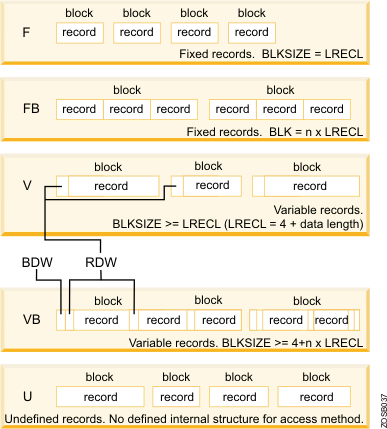
\includegraphics{zOSB037.png}

See \href{http://en.wikipedia.org/wiki/Data\_set\_(IBM\_mainframe}{http://en.wikipedia.org/wiki/Data\_set\_(IBM\_mainframe})

See \href{http://www.simotime.com/vrecex01.htm}{http://www.simotime.com/vrecex01.htm}

There are three relevant encoding possibilities. These are the COBOL ``RECFM''
options in the JCL for the file. Each record is preceded by a
Record Descriptor Word (RDW).

\code{V}   Variable.
\begin{quote}

The four bytes preceding the logical record is the Record Descriptor Word. The content is as follows.

\begin{tabulary}{\linewidth}{|L|L|}
\hline
\textsf{\relax 
Bytes
} & \textsf{\relax 
Description
}\\
\hline
1-2
 & 
This is the length of the logical record plus the length of the four-byte Descriptor Word.
\\

3-4
 & 
Usually low values
\\
\hline\end{tabulary}

\end{quote}

\code{VB}  Variable Blocked.
\begin{quote}

The four bytes preceding the logical record (Descriptor Word) are as follows.

\begin{tabulary}{\linewidth}{|L|L|}
\hline
\textsf{\relax 
Bytes
} & \textsf{\relax 
Description
}\\
\hline
1-2
 & 
This is the length of the logical record plus the length of the four-byte Descriptor Word.
\\

3-4
 & 
The length of the block including four-byte Descriptor Word.
\\
\hline\end{tabulary}

\end{quote}

A block can have multiple records in it. The block length must be \textgreater{}= record length.

\code{VBS}     Variable Blocked Spanned.
\begin{quote}

The four bytes preceding the logical record is the Segment Descriptor Word. The content is as follows.

\begin{tabulary}{\linewidth}{|L|L|}
\hline
\textsf{\relax 
Bytes
} & \textsf{\relax 
Description
}\\
\hline
1-2
 & 
This is the length of the logical record plus the length of the four-byte Descriptor Word.
\\

3
 & 
Segment Control Codes: see below.
\\

4
 & 
Low value, reserved for future use
\\
\hline\end{tabulary}


Segment Control Code

\begin{tabulary}{\linewidth}{|L|L|}
\hline
\textsf{\relax 
Value
} & \textsf{\relax 
Relative position of segment
}\\
\hline
00
 & 
A complete logical record
\\

01
 & 
The first segment of a multiple segments record
\\

02
 & 
The last segment of a multiple segments record
\\

03
 & 
A middle segment of a multiple segments record
\\
\hline\end{tabulary}

\end{quote}

This RECFM detail must be provided as part of opening the workbook/sheet so that rows can be
properly located within the content.

We've added a series of RECFM classes as a \textbf{Strategy} to
read files with variable length records.


\subsubsection{Low-Level Split Processing}
\label{cobol:low-level-split-processing}
We may have a need to split an EBCDIC file, similar to the Posix \code{split} command.
This is done using \code{cobol.RECFM} parsers to read records and write to
new file(s).

A splitter looks like this:

\begin{Verbatim}[commandchars=\\\{\}]
import itertools
import stringray.cobol
import collections
import pprint

batch\PYGZus{}size= 1000
counts= collections.defaultdict(int)
with open( \PYGZdq{}some\PYGZus{}file.schema\PYGZdq{}, \PYGZdq{}rb\PYGZdq{} ) as source:
    reader= stringray.cobol.RECFM\PYGZus{}VB( source ).bdw\PYGZus{}iter()
    batches= itertools.groupby( enumerate(reader), lambda x: x[0]//batch\PYGZus{}size ):
    for group, group\PYGZus{}iter in batches:
        with open( \PYGZdq{}some\PYGZus{}file\PYGZus{}\PYGZob{}0\PYGZcb{}.schema\PYGZdq{}.format(group), \PYGZdq{}wb\PYGZdq{} ) as target:
        for id, row in group\PYGZus{}iter:
            target.write( row )
            counts[\PYGZsq{}rows\PYGZsq{}] += 1
            counts[str(group)] += 1
pprint.pprint( dict(counts) )
\end{Verbatim}

There are several possible variations on the construction of the \code{reader} object.
\begin{itemize}
\item {} 
cobol.RECFM\_F( source ).record\_iter() -- result is RECFM\_F.

\item {} 
cobol.RECFM\_F( source ).rdw\_iter() -- result is RECFM\_V; RDW's have been added.

\item {} 
cobol.RECFM\_V( source ).rdw\_iter() -- result is RECFM\_V; RDW's have been preserved.

\item {} 
cobol.RECFM\_VB( source ).rdw\_iter() -- result is RECFM\_V; RDW's have been preserved;
BDW's have been discarded.

\item {} 
cobol.RECFM\_VB( source ).bdw\_iter() -- result is RECFM\_VB; BDW's and RDW's have been
preserved. The batch size is the number of blocks, not the number of records.

\end{itemize}


\subsubsection{The Bad Data Problem}
\label{cobol:the-bad-data-problem}
Even with a {\hyperref[sheet:sheet.LazyRow]{\code{sheet.LazyRow}}}, we have to be tolerant of COBOL data which doesn't match
the schema. The {\hyperref[cobol_defs:cobol.defs.Usage.create_func]{\code{cobol.defs.Usage.create\_func()}}} function may encounter an exception.
If so, then a {\hyperref[cobol_defs:cobol.defs.ErrorCell]{\code{cobol.defs.ErrorCell}}} is created instead of the class
defined by the Usage and Picture classes.

The {\hyperref[cobol_defs:cobol.defs.ErrorCell]{\code{cobol.defs.ErrorCell}}} includes the raw bytes, but a value of \code{None}.


\subsection{COBOL Implementation}
\label{cobol:cobol-implementation}\label{cobol:cobol-impl}
These are the modules that extend the core functionality of Stingray
to handle COBOL files and EBCDIC data.


\subsubsection{COBOL Package -- Extend Schema to Handle EBCDIC}
\label{cobol_init:cobol-init}\label{cobol_init:cobol-package-extend-schema-to-handle-ebcdic}\label{cobol_init::doc}
The COBOL package is a (large) Python \code{\_\_init\_\_.py} module which
includes much of the public API for working with COBOL files.

This module extends Stingray in several directions.
\begin{itemize}
\item {} 
A new {\hyperref[schema:schema.Attribute]{\code{schema.Attribute}}} subclass, {\hyperref[cobol_init:cobol.RepeatingAttribute]{\code{cobol.RepeatingAttribute}}}.

\item {} 
A handy {\hyperref[cobol_init:cobol.dump]{\code{cobol.dump()}}} function.

\item {} 
The hierarchy of classes based on {\hyperref[cobol_init:cobol.COBOL_File]{\code{cobol.COBOL\_File}}} which provide
more sophisticated COBOL-based workbooks.

\end{itemize}

Within the package we have the {\hyperref[cobol_loader:module-cobol.loader]{\code{cobol.loader}}} module which parses DDE's
to create a schema.


\paragraph{Module Overheads}
\label{cobol_init:module-overheads}\label{cobol_init:module-cobol}\index{cobol (module)}
We depend on {\hyperref[cell:module-cell]{\code{cell}}}, {\hyperref[schema:module-schema]{\code{schema}}}, and {\hyperref[workbook/init:module-workbook]{\code{workbook}}}.
We'll also import one class definition from {\hyperref[cobol_defs:module-cobol.defs]{\code{cobol.defs}}}.

\begin{Verbatim}[commandchars=\\\{\}]
\PYG{l+s+sd}{\PYGZdq{}\PYGZdq{}\PYGZdq{}stingray.cobol \PYGZhy{}\PYGZhy{} Extend the core Stingray definitions to handle COBOL}
\PYG{l+s+sd}{DDE\PYGZsq{}s and COBOL files, including packed decimal and EBCDIC data.}
\PYG{l+s+sd}{\PYGZdq{}\PYGZdq{}\PYGZdq{}}
\PYG{k+kn}{import} \PYG{n+nn}{codecs}
\PYG{k+kn}{import} \PYG{n+nn}{struct}
\PYG{k+kn}{import} \PYG{n+nn}{decimal}
\PYG{k+kn}{import} \PYG{n+nn}{warnings}
\PYG{k+kn}{import} \PYG{n+nn}{pprint}
\PYG{k+kn}{import} \PYG{n+nn}{logging}

\PYG{k+kn}{import} \PYG{n+nn}{stingray.schema}
\PYG{k+kn}{import} \PYG{n+nn}{stingray.sheet}
\PYG{k+kn}{from} \PYG{n+nn}{stingray.workbook.fixed} \PYG{k+kn}{import} \PYG{n}{Fixed\PYGZus{}Workbook}


\PYG{k+kn}{from} \PYG{n+nn}{stingray.cobol.defs} \PYG{k+kn}{import} \PYG{n}{TextCell}
\end{Verbatim}


\paragraph{RepeatingAttribute Subclasses of Attribute}
\label{cobol_init:repeatingattribute-subclasses-of-attribute}
Two new {\hyperref[schema:schema.Attribute]{\code{schema.Attribute}}} subclasses are required to carry all the
additional attribute information developed during COBOL DDE parsing.

An attribute that has an \code{OCCURS} clause (or who's parent has an \code{OCCURS} clause)
can accept an {\hyperref[cobol_init:cobol.RepeatingAttribute.index]{\code{cobol.RepeatingAttribute.index()}}} method to provide index values used to compute
effective offsets.

There are two variants.
\begin{itemize}
\item {} 
The initial, immutable, {\hyperref[cobol_init:cobol.RepeatingAttribute]{\code{cobol.RepeatingAttribute}}} as parsed.

\item {} 
A working {\hyperref[cobol_init:cobol.IndexedAttribute]{\code{cobol.IndexedAttribute}}}. This is a subclass of
{\hyperref[cobol_init:cobol.RepeatingAttribute]{\code{cobol.RepeatingAttribute}}} and it contains partial or complete
indexing. Partial indexing means that a tuple is built by
{\hyperref[cobol_init:cobol.COBOL_File.row_get]{\code{cobol.COBOL\_File.row\_get()}}}. Full indexing means that a single
\code{Cell} can be built.

\end{itemize}

\begin{Verbatim}[commandchars=\\\{\}]
http://yuml.me/diagram/scruffy;/class/
\PYGZsh{}cobol.attribute,
[Attribute]\PYGZca{}[RepeatingAttribute],
[Schema]\PYGZlt{}\PYGZgt{}\PYGZhy{}[Attribute],
[Fixed\PYGZus{}Workbook]\PYGZhy{}uses\PYGZhy{}\PYGZgt{}[Attribute],
[Fixed\PYGZus{}Workbook]\PYGZca{}[COBOL\PYGZus{}File],
[COBOL\PYGZus{}File]\PYGZhy{}uses\PYGZhy{}\PYGZgt{}[RepeatingAttribute].
\end{Verbatim}

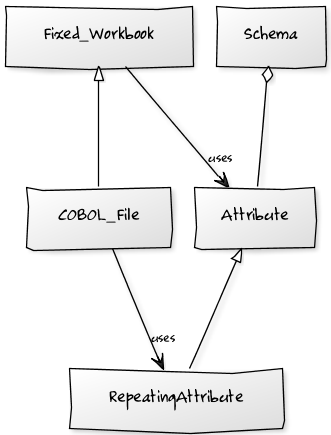
\includegraphics{cobol_attribute.png}

In order to fetch data for an ODO \code{OCCURS} element, the attribute offsets and sizes
cannot \textbf{all} be computed during parsing.
They must be computed lazily during data fetching. The {\hyperref[cobol_init:cobol.ODO_LazyRow]{\code{cobol.ODO\_LazyRow}}}
class handles the Occurs Depending On situation.

Here are the attributes inherited from {\hyperref[schema:schema.Attribute]{\code{schema.Attribute}}}.
\index{name (in module cobol)}

\begin{fulllineitems}
\phantomsection\label{cobol_init:cobol.name}\pysigline{\code{cobol.}\bfcode{name}}
The attribute name. Typically always available for most kinds of schema.

\end{fulllineitems}

\index{create (in module cobol)}

\begin{fulllineitems}
\phantomsection\label{cobol_init:cobol.create}\pysigline{\code{cobol.}\bfcode{create}}
Cell class to create.  If omitted, the class-level
\code{Attribute.default\_cell} will be used.
By default, this refers to {\hyperref[cell:cell.TextCell]{\code{cell.TextCell}}}.

\end{fulllineitems}

\index{position (in module cobol)}

\begin{fulllineitems}
\phantomsection\label{cobol_init:cobol.position}\pysigline{\code{cobol.}\bfcode{position}}
Optional sequential position. This is set by the {\hyperref[schema:schema.Schema]{\code{schema.Schema}}}
that contains this object.

\end{fulllineitems}


The additional values commonly provided by simple fixed format file schemata.
These can't be treated as simple values, however, since they're
clearly changed based on the ODO issues.
\index{size (in module cobol)}

\begin{fulllineitems}
\phantomsection\label{cobol_init:cobol.size}\pysigline{\code{cobol.}\bfcode{size}}
Size within the buffer.

\end{fulllineitems}


These two properties over overridden by the {\hyperref[cobol_init:cobol.IndexedAttribute]{\code{cobol.IndexedAttribute}}} subclass;
this is created by the {\hyperref[cobol_init:cobol.RepeatingAttribute.index]{\code{cobol.RepeatingAttribute.index()}}} method.
The superclass versions are simple a delegation to the DDE.
If {\hyperref[cobol_init:cobol.RepeatingAttribute.index]{\code{cobol.RepeatingAttribute.index()}}} is used, the subclass object is built
where these values come from the \code{index} method results.
\index{dimensionality (in module cobol)}

\begin{fulllineitems}
\phantomsection\label{cobol_init:cobol.dimensionality}\pysigline{\code{cobol.}\bfcode{dimensionality}}
A tuple of DDE's that defines the dimensionality pushed down to this
item through the COBOL DDE hierarchy.

This meay be set by the {\hyperref[cobol_init:cobol.RepeatingAttribute.index]{\code{cobol.RepeatingAttribute.index()}}} method.

\end{fulllineitems}

\index{offset (in module cobol)}

\begin{fulllineitems}
\phantomsection\label{cobol_init:cobol.offset}\pysigline{\code{cobol.}\bfcode{offset}}
Optional offset into a buffer. This may be statically defined,
or it may be dynamic because of variably-located data supporting
the Occurs Depends On.

This meay be set by the {\hyperref[cobol_init:cobol.RepeatingAttribute.index]{\code{cobol.RepeatingAttribute.index()}}} method.

\end{fulllineitems}


This subclass introduces yet more attribute-like properties that simply
delegate to the DDE.
\index{dde (in module cobol)}

\begin{fulllineitems}
\phantomsection\label{cobol_init:cobol.dde}\pysigline{\code{cobol.}\bfcode{dde}}
A weakref to a \code{cobol.loader.DDE} object.

\end{fulllineitems}

\index{path (in module cobol)}

\begin{fulllineitems}
\phantomsection\label{cobol_init:cobol.path}\pysigline{\code{cobol.}\bfcode{path}}
The ''.''-separated path from top-level name to this element's name.

\end{fulllineitems}

\index{usage (in module cobol)}

\begin{fulllineitems}
\phantomsection\label{cobol_init:cobol.usage}\pysigline{\code{cobol.}\bfcode{usage}}
The original DDE.usage object, an instance of {\hyperref[cobol_defs:cobol.defs.Usage]{\code{cobol.defs.Usage}}}

\end{fulllineitems}

\index{redefines (in module cobol)}

\begin{fulllineitems}
\phantomsection\label{cobol_init:cobol.redefines}\pysigline{\code{cobol.}\bfcode{redefines}}
The original DDE.allocation object, an instance of \code{cobol.loader.Allocation}

\end{fulllineitems}

\index{picture (in module cobol)}

\begin{fulllineitems}
\phantomsection\label{cobol_init:cobol.picture}\pysigline{\code{cobol.}\bfcode{picture}}
The original DDE.picture object, an instance of \code{cobol.defs.Picture}

\end{fulllineitems}

\index{size\_scale\_precision (in module cobol)}

\begin{fulllineitems}
\phantomsection\label{cobol_init:cobol.size_scale_precision}\pysigline{\code{cobol.}\bfcode{size\_scale\_precision}}
The original DDE.sizeScalePrecision object, a tuple with size, scale and precision derived
from the picture.

\end{fulllineitems}

\index{RepeatingAttribute (class in cobol)}

\begin{fulllineitems}
\phantomsection\label{cobol_init:cobol.RepeatingAttribute}\pysigline{\strong{class }\code{cobol.}\bfcode{RepeatingAttribute}}
An attribute with dimensionality. Not all COBOL items repeat.

\end{fulllineitems}


\begin{Verbatim}[commandchars=\\\{\}]
\PYG{k}{class} \PYG{n+nc}{RepeatingAttribute}\PYG{p}{(} \PYG{n}{stingray}\PYG{o}{.}\PYG{n}{schema}\PYG{o}{.}\PYG{n}{Attribute} \PYG{p}{)}\PYG{p}{:}
    \PYG{l+s+sd}{\PYGZdq{}\PYGZdq{}\PYGZdq{}An attribute with dimensionality. Not all COBOL items repeat.}

\PYG{l+s+sd}{    An \PYGZdq{}OCCURS\PYGZdq{} clause will define repeating values.}
\PYG{l+s+sd}{    An \PYGZdq{}OCCURS DEPENDING ON\PYGZdq{} clause may define variably located values.}
\PYG{l+s+sd}{    \PYGZdq{}\PYGZdq{}\PYGZdq{}}
    \PYG{n}{default\PYGZus{}cell}\PYG{o}{=} \PYG{n}{TextCell}
    \PYG{k}{def} \PYG{n+nf}{\PYGZus{}\PYGZus{}init\PYGZus{}\PYGZus{}}\PYG{p}{(}\PYG{n+nb+bp}{self}\PYG{p}{,} \PYG{n}{name}\PYG{p}{,} \PYG{n}{dde}\PYG{p}{,} \PYG{n}{offset}\PYG{o}{=}\PYG{n+nb+bp}{None}\PYG{p}{,} \PYG{n}{size}\PYG{o}{=}\PYG{n+nb+bp}{None}\PYG{p}{,} \PYG{n}{create}\PYG{o}{=}\PYG{n+nb+bp}{None}\PYG{p}{,} \PYG{n}{position}\PYG{o}{=}\PYG{n+nb+bp}{None}\PYG{p}{,} \PYG{o}{*}\PYG{o}{*}\PYG{n}{kw}\PYG{p}{)}\PYG{p}{:}
        \PYG{n+nb+bp}{self}\PYG{o}{.}\PYG{n}{dde}\PYG{o}{=} \PYG{n}{dde}
        \PYG{n+nb+bp}{self}\PYG{o}{.}\PYG{n}{name}\PYG{p}{,} \PYG{n+nb+bp}{self}\PYG{o}{.}\PYG{n}{size}\PYG{p}{,} \PYG{n+nb+bp}{self}\PYG{o}{.}\PYG{n}{create}\PYG{p}{,} \PYG{n+nb+bp}{self}\PYG{o}{.}\PYG{n}{position} \PYG{o}{=} \PYG{n}{name}\PYG{p}{,} \PYG{n}{size}\PYG{p}{,} \PYG{n}{create}\PYG{p}{,} \PYG{n}{position}
        \PYG{k}{if} \PYG{o+ow}{not} \PYG{n+nb+bp}{self}\PYG{o}{.}\PYG{n}{create}\PYG{p}{:}
            \PYG{n+nb+bp}{self}\PYG{o}{.}\PYG{n}{create}\PYG{o}{=} \PYG{n+nb+bp}{self}\PYG{o}{.}\PYG{n}{default\PYGZus{}cell}
        \PYG{k}{if} \PYG{n}{offset} \PYG{o+ow}{is} \PYG{o+ow}{not} \PYG{n+nb+bp}{None}\PYG{p}{:}
            \PYG{n}{warnings}\PYG{o}{.}\PYG{n}{warn}\PYG{p}{(} \PYG{l+s}{\PYGZdq{}}\PYG{l+s}{Offset \PYGZob{}0\PYGZcb{} is ignored; \PYGZob{}1\PYGZcb{} used}\PYG{l+s}{\PYGZdq{}}\PYG{o}{.}\PYG{n}{format}\PYG{p}{(}\PYG{n}{offset}\PYG{p}{,} \PYG{n+nb+bp}{self}\PYG{o}{.}\PYG{n}{dde}\PYG{p}{(}\PYG{p}{)}\PYG{o}{.}\PYG{n}{offset}\PYG{p}{)}\PYG{p}{,} \PYG{n}{stacklevel}\PYG{o}{=}\PYG{l+m+mi}{2} \PYG{p}{)}
        \PYG{n+nb+bp}{self}\PYG{o}{.}\PYG{n}{\PYGZus{}\PYGZus{}dict\PYGZus{}\PYGZus{}}\PYG{o}{.}\PYG{n}{update}\PYG{p}{(} \PYG{n}{kw} \PYG{p}{)}
    \PYG{k}{def} \PYG{n+nf}{\PYGZus{}\PYGZus{}repr\PYGZus{}\PYGZus{}}\PYG{p}{(} \PYG{n+nb+bp}{self} \PYG{p}{)}\PYG{p}{:}
        \PYG{n}{dim}\PYG{o}{=} \PYG{l+s}{\PYGZdq{}}\PYG{l+s}{, }\PYG{l+s}{\PYGZdq{}}\PYG{o}{.}\PYG{n}{join}\PYG{p}{(} \PYG{n+nb}{map}\PYG{p}{(} \PYG{n+nb}{repr}\PYG{p}{,} \PYG{n+nb+bp}{self}\PYG{o}{.}\PYG{n}{dimensionality} \PYG{p}{)} \PYG{p}{)}
        \PYG{k}{return} \PYG{l+s}{\PYGZdq{}}\PYG{l+s}{Attribute( name=\PYGZob{}0.name!r\PYGZcb{}, position=\PYGZob{}0.position\PYGZcb{}, offset=\PYGZob{}0.offset\PYGZcb{}, size=\PYGZob{}0.size\PYGZcb{}, dimensionality=(\PYGZob{}1\PYGZcb{}) )}\PYG{l+s}{\PYGZdq{}}\PYG{o}{.}\PYG{n}{format}\PYG{p}{(}
            \PYG{n+nb+bp}{self}\PYG{p}{,} \PYG{n}{dim} \PYG{p}{)}
\end{Verbatim}
\index{index() (cobol.RepeatingAttribute method)}

\begin{fulllineitems}
\phantomsection\label{cobol_init:cobol.RepeatingAttribute.index}\pysiglinewithargsret{\code{RepeatingAttribute.}\bfcode{index}}{\emph{*values}}{}
If the number of index values matches the dimensionality, we'll return a tweaked
attribute which has just the offset required and a dimensionality of \code{tuple()}.

If the number of index values is insufficient, we'll return a tweaked attribute
with which has the starting offset and the dimensions left otherwise unspecified.

If the number of index values is excessive, we'll attempt to pop from an empty
list.

Note that {\hyperref[cobol_init:cobol.RepeatingAttribute.index]{\code{cobol.RepeatingAttribute.index()}}} is applied incrementally when the application supplies some
of the indices.
\begin{itemize}
\item {} 
First, an application can supply some of the indices, creating
{\hyperref[cobol_init:cobol.IndexedAttribute]{\code{cobol.IndexedAttribute}}} with an initial offset.

\item {} 
Second, the {\hyperref[cobol_init:cobol.COBOL_File]{\code{COBOL\_File}}} will supply any remaining indices,
creating yet more temporary  {\hyperref[cobol_init:cobol.IndexedAttribute]{\code{cobol.IndexedAttribute}}} based on the initial offset.

\end{itemize}

\end{fulllineitems}


\begin{Verbatim}[commandchars=\\\{\}]
\PYG{k}{def} \PYG{n+nf}{index}\PYG{p}{(} \PYG{n+nb+bp}{self}\PYG{p}{,} \PYG{o}{*}\PYG{n}{values} \PYG{p}{)}\PYG{p}{:}
    \PYG{l+s+sd}{\PYGZdq{}\PYGZdq{}\PYGZdq{}\PYGZdq{}Apply possibly incomplete index values to an attribute.}
\PYG{l+s+sd}{    We do this by cloning this attribute and setting a modified}
\PYG{l+s+sd}{    dimensionality and offset.}

\PYG{l+s+sd}{    :param values: 0\PYGZhy{}based index values.  Yes, legacy COBOL language is 1\PYGZhy{}based.}
\PYG{l+s+sd}{        For Python applications, zero\PYGZhy{}based makes more sense.}
\PYG{l+s+sd}{    :returns: A :py:class:{}`cobol.IndexedAttribute{}` copy, with modified offset}
\PYG{l+s+sd}{    and dimensionality that can be used with :py:meth:{}`COBOL\PYGZus{}File.row\PYGZus{}get{}`.}
\PYG{l+s+sd}{    \PYGZdq{}\PYGZdq{}\PYGZdq{}}
    \PYG{k}{assert} \PYG{n}{values}\PYG{p}{,} \PYG{l+s}{\PYGZdq{}}\PYG{l+s}{Missing index values}\PYG{l+s}{\PYGZdq{}}
    \PYG{c}{\PYGZsh{} Original values for a RepeatingAttribute}
    \PYG{c}{\PYGZsh{} Modified values for an IndexedAttribute}
    \PYG{n}{offset}\PYG{o}{=} \PYG{n+nb+bp}{self}\PYG{o}{.}\PYG{n}{offset}
    \PYG{n}{dim\PYGZus{}list}\PYG{o}{=} \PYG{n+nb}{list}\PYG{p}{(}\PYG{n+nb+bp}{self}\PYG{o}{.}\PYG{n}{dimensionality}\PYG{p}{)}
    \PYG{c}{\PYGZsh{} Apply given index values.}
    \PYG{n}{val\PYGZus{}list}\PYG{o}{=} \PYG{n+nb}{list}\PYG{p}{(}\PYG{n}{values}\PYG{p}{)}
    \PYG{k}{while} \PYG{n}{val\PYGZus{}list}\PYG{p}{:}
        \PYG{n}{index}\PYG{o}{=} \PYG{n}{val\PYGZus{}list}\PYG{o}{.}\PYG{n}{pop}\PYG{p}{(}\PYG{l+m+mi}{0}\PYG{p}{)}
        \PYG{n}{dim}\PYG{o}{=} \PYG{n}{dim\PYGZus{}list}\PYG{o}{.}\PYG{n}{pop}\PYG{p}{(}\PYG{l+m+mi}{0}\PYG{p}{)}
        \PYG{n}{offset} \PYG{o}{+}\PYG{o}{=} \PYG{n}{dim}\PYG{o}{.}\PYG{n}{size} \PYG{o}{*} \PYG{n}{index}
    \PYG{c}{\PYGZsh{} Build new subclass object with indexes applied.}
    \PYG{n}{clone}\PYG{o}{=} \PYG{n}{IndexedAttribute}\PYG{p}{(} \PYG{n+nb+bp}{self}\PYG{p}{,} \PYG{n}{offset}\PYG{p}{,} \PYG{n}{dim\PYGZus{}list} \PYG{p}{)}
    \PYG{k}{return} \PYG{n}{clone}
\end{Verbatim}

With this, a \code{row.cell(schema.get('name').index(i))} will compute a proper offset.

We ``clone'' the attribute to assure that each time we apply (or don't apply)
the index, nothing stateful will have happened to the original immutable attribute
definition.

Note that an incomplete set of index values forces the underlying
workbook to create a Python tuple (or tuple of tuples) structure to
contain all the requested values. See {\hyperref[cobol_init:cobol.COBOL_File.row_get]{\code{cobol.COBOL\_File.row\_get()}}}.

The additional properties which are simply shortcuts so that a
generic {\hyperref[cobol_init:cobol.RepeatingAttribute]{\code{cobol.RepeatingAttribute}}} has access to the DDE details.

\begin{Verbatim}[commandchars=\\\{\}]
\PYG{n+nd}{@property}
\PYG{k}{def} \PYG{n+nf}{dimensionality}\PYG{p}{(}\PYG{n+nb+bp}{self}\PYG{p}{)}\PYG{p}{:}
    \PYG{l+s+sd}{\PYGZdq{}\PYGZdq{}\PYGZdq{}tuple of parent DDE\PYGZsq{}s. Baseline value; no indexes applied.\PYGZdq{}\PYGZdq{}\PYGZdq{}}
    \PYG{k}{return} \PYG{n+nb+bp}{self}\PYG{o}{.}\PYG{n}{dde}\PYG{p}{(}\PYG{p}{)}\PYG{o}{.}\PYG{n}{dimensionality}
\PYG{n+nd}{@property}
\PYG{k}{def} \PYG{n+nf}{offset}\PYG{p}{(}\PYG{n+nb+bp}{self}\PYG{p}{)}\PYG{p}{:}
    \PYG{l+s+sd}{\PYGZdq{}\PYGZdq{}\PYGZdq{}Baseline value; no indexes applied.\PYGZdq{}\PYGZdq{}\PYGZdq{}}
    \PYG{k}{return} \PYG{n+nb+bp}{self}\PYG{o}{.}\PYG{n}{dde}\PYG{p}{(}\PYG{p}{)}\PYG{o}{.}\PYG{n}{offset}
\PYG{n+nd}{@property}
\PYG{k}{def} \PYG{n+nf}{path}\PYG{p}{(}\PYG{n+nb+bp}{self}\PYG{p}{)}\PYG{p}{:}
    \PYG{k}{return} \PYG{n+nb+bp}{self}\PYG{o}{.}\PYG{n}{dde}\PYG{p}{(}\PYG{p}{)}\PYG{o}{.}\PYG{n}{pathTo}\PYG{p}{(}\PYG{p}{)}
\PYG{n+nd}{@property}
\PYG{k}{def} \PYG{n+nf}{usage}\PYG{p}{(}\PYG{n+nb+bp}{self}\PYG{p}{)}\PYG{p}{:}
    \PYG{k}{return} \PYG{n+nb+bp}{self}\PYG{o}{.}\PYG{n}{dde}\PYG{p}{(}\PYG{p}{)}\PYG{o}{.}\PYG{n}{usage}
\PYG{n+nd}{@property}
\PYG{k}{def} \PYG{n+nf}{redefines}\PYG{p}{(}\PYG{n+nb+bp}{self}\PYG{p}{)}\PYG{p}{:}
    \PYG{k}{return} \PYG{n+nb+bp}{self}\PYG{o}{.}\PYG{n}{dde}\PYG{p}{(}\PYG{p}{)}\PYG{o}{.}\PYG{n}{allocation}
\PYG{n+nd}{@property}
\PYG{k}{def} \PYG{n+nf}{picture}\PYG{p}{(}\PYG{n+nb+bp}{self}\PYG{p}{)}\PYG{p}{:}
    \PYG{k}{return} \PYG{n+nb+bp}{self}\PYG{o}{.}\PYG{n}{dde}\PYG{p}{(}\PYG{p}{)}\PYG{o}{.}\PYG{n}{picture}
\PYG{n+nd}{@property}
\PYG{k}{def} \PYG{n+nf}{size\PYGZus{}scale\PYGZus{}precision}\PYG{p}{(}\PYG{n+nb+bp}{self}\PYG{p}{)}\PYG{p}{:}
    \PYG{k}{return} \PYG{n+nb+bp}{self}\PYG{o}{.}\PYG{n}{dde}\PYG{p}{(}\PYG{p}{)}\PYG{o}{.}\PYG{n}{sizeScalePrecision}
\end{Verbatim}
\index{IndexedAttribute (class in cobol)}

\begin{fulllineitems}
\phantomsection\label{cobol_init:cobol.IndexedAttribute}\pysigline{\strong{class }\code{cobol.}\bfcode{IndexedAttribute}}
The IndexedAttribute is a subclass of {\hyperref[cobol_init:cobol.RepeatingAttribute]{\code{cobol.RepeatingAttribute}}}
with (some) indices applied. Since this inherits the {\hyperref[cobol_init:cobol.RepeatingAttribute.index]{\code{cobol.RepeatingAttribute.index()}}}
method, we can apply indices incrementally.

This class is not built directly, but only created by {\hyperref[cobol_init:cobol.RepeatingAttribute.index]{\code{cobol.RepeatingAttribute.index()}}}
with some (or all) indices applied.

\end{fulllineitems}


\begin{Verbatim}[commandchars=\\\{\}]
\PYG{k}{class} \PYG{n+nc}{IndexedAttribute}\PYG{p}{(} \PYG{n}{RepeatingAttribute} \PYG{p}{)}\PYG{p}{:}
    \PYG{l+s+sd}{\PYGZdq{}\PYGZdq{}\PYGZdq{}An attribute with dimensionality and indexes applied.}
\PYG{l+s+sd}{    This must be built from a :py:class:{}`cobol.RepeatingAttribute{}`. It will copy}
\PYG{l+s+sd}{    some attributes in an effort to somewhat improve efficiency.}
\PYG{l+s+sd}{    \PYGZdq{}\PYGZdq{}\PYGZdq{}}
    \PYG{n}{default\PYGZus{}cell}\PYG{o}{=} \PYG{n}{TextCell}
    \PYG{k}{def} \PYG{n+nf}{\PYGZus{}\PYGZus{}init\PYGZus{}\PYGZus{}}\PYG{p}{(}\PYG{n+nb+bp}{self}\PYG{p}{,} \PYG{n}{base}\PYG{p}{,} \PYG{n}{offset}\PYG{p}{,} \PYG{n}{dimensionality} \PYG{p}{)}\PYG{p}{:}
        \PYG{n+nb+bp}{self}\PYG{o}{.}\PYG{n}{dde}\PYG{o}{=} \PYG{n}{base}\PYG{o}{.}\PYG{n}{dde}
        \PYG{n+nb+bp}{self}\PYG{o}{.}\PYG{n}{name}\PYG{p}{,} \PYG{n+nb+bp}{self}\PYG{o}{.}\PYG{n}{size}\PYG{p}{,} \PYG{n+nb+bp}{self}\PYG{o}{.}\PYG{n}{create}\PYG{p}{,} \PYG{n+nb+bp}{self}\PYG{o}{.}\PYG{n}{position} \PYG{o}{=} \PYG{n}{base}\PYG{o}{.}\PYG{n}{name}\PYG{p}{,} \PYG{n}{base}\PYG{o}{.}\PYG{n}{size}\PYG{p}{,} \PYG{n}{base}\PYG{o}{.}\PYG{n}{create}\PYG{p}{,} \PYG{n}{base}\PYG{o}{.}\PYG{n}{position}
        \PYG{n+nb+bp}{self}\PYG{o}{.}\PYG{n}{\PYGZus{}offset}\PYG{o}{=} \PYG{n}{offset}
        \PYG{n+nb+bp}{self}\PYG{o}{.}\PYG{n}{\PYGZus{}dimensionality}\PYG{o}{=} \PYG{n}{dimensionality}
    \PYG{n+nd}{@property}
    \PYG{k}{def} \PYG{n+nf}{dimensionality}\PYG{p}{(}\PYG{n+nb+bp}{self}\PYG{p}{)}\PYG{p}{:}
        \PYG{l+s+sd}{\PYGZdq{}\PYGZdq{}\PYGZdq{}tuple of DDE\PYGZsq{}s; Set by {}`{}`attribute.index(){}`{}`.\PYGZdq{}\PYGZdq{}\PYGZdq{}}
        \PYG{k}{return} \PYG{n+nb+bp}{self}\PYG{o}{.}\PYG{n}{\PYGZus{}dimensionality}
    \PYG{n+nd}{@property}
    \PYG{k}{def} \PYG{n+nf}{offset}\PYG{p}{(}\PYG{n+nb+bp}{self}\PYG{p}{)}\PYG{p}{:}
        \PYG{l+s+sd}{\PYGZdq{}\PYGZdq{}\PYGZdq{}Set by {}`{}`attribute.index(){}`{}`.\PYGZdq{}\PYGZdq{}\PYGZdq{}}
        \PYG{k}{return} \PYG{n+nb+bp}{self}\PYG{o}{.}\PYG{n}{\PYGZus{}offset}
\end{Verbatim}


\paragraph{COBOL LazyRow}
\label{cobol_init:cobol-lazyrow}
The {\hyperref[sheet:sheet.LazyRow]{\code{sheet.LazyRow}}} class is blissfully unaware of the need to compute
sizes and offsets for COBOL.
\index{ODO\_LazyRow (class in cobol)}

\begin{fulllineitems}
\phantomsection\label{cobol_init:cobol.ODO_LazyRow}\pysigline{\strong{class }\code{cobol.}\bfcode{ODO\_LazyRow}}
This subclass of {\hyperref[sheet:sheet.LazyRow]{\code{sheet.LazyRow}}} to provide add the feature to recompute sizes
and offsets in the case of a variable-located DDE due to an Occurs Depending On.

\end{fulllineitems}


\begin{Verbatim}[commandchars=\\\{\}]
\PYG{k}{class} \PYG{n+nc}{ODO\PYGZus{}LazyRow}\PYG{p}{(} \PYG{n}{stingray}\PYG{o}{.}\PYG{n}{sheet}\PYG{o}{.}\PYG{n}{LazyRow} \PYG{p}{)}\PYG{p}{:}
    \PYG{l+s+sd}{\PYGZdq{}\PYGZdq{}\PYGZdq{}If the DDE is variably\PYGZhy{}located, tweak the sizes and offsets.\PYGZdq{}\PYGZdq{}\PYGZdq{}}

    \PYG{k}{def} \PYG{n+nf}{\PYGZus{}\PYGZus{}init\PYGZus{}\PYGZus{}}\PYG{p}{(} \PYG{n+nb+bp}{self}\PYG{p}{,} \PYG{n}{sheet}\PYG{p}{,} \PYG{o}{*}\PYG{o}{*}\PYG{n}{state} \PYG{p}{)}\PYG{p}{:}
        \PYG{l+s+sd}{\PYGZdq{}\PYGZdq{}\PYGZdq{}Build the row from the bytes.}

\PYG{l+s+sd}{        :param sheet: the containing sheet.}
\PYG{l+s+sd}{        :param **state: worksheet\PYGZhy{}specific state value to save.}
\PYG{l+s+sd}{        \PYGZdq{}\PYGZdq{}\PYGZdq{}}
        \PYG{n+nb}{super}\PYG{p}{(}\PYG{p}{)}\PYG{o}{.}\PYG{n}{\PYGZus{}\PYGZus{}init\PYGZus{}\PYGZus{}}\PYG{p}{(} \PYG{n}{sheet}\PYG{p}{,} \PYG{o}{*}\PYG{o}{*}\PYG{n}{state} \PYG{p}{)}
        \PYG{k}{for} \PYG{n}{dde} \PYG{o+ow}{in} \PYG{n+nb+bp}{self}\PYG{o}{.}\PYG{n}{sheet}\PYG{o}{.}\PYG{n}{schema}\PYG{o}{.}\PYG{n}{info}\PYG{o}{.}\PYG{n}{get}\PYG{p}{(}\PYG{l+s}{\PYGZsq{}}\PYG{l+s}{dde}\PYG{l+s}{\PYGZsq{}}\PYG{p}{,}\PYG{p}{[}\PYG{p}{]}\PYG{p}{)}\PYG{p}{:}
            \PYG{k}{if} \PYG{n}{dde}\PYG{o}{.}\PYG{n}{variably\PYGZus{}located}\PYG{p}{:}
                \PYG{n}{dde}\PYG{o}{.}\PYG{n}{setSizeAndOffset}\PYG{p}{(}\PYG{n+nb+bp}{self}\PYG{p}{)}
            \PYG{n+nb+bp}{self}\PYG{o}{.}\PYG{n}{\PYGZus{}size}\PYG{o}{=} \PYG{n}{dde}\PYG{o}{.}\PYG{n}{totalSize}
        \PYG{k}{else}\PYG{p}{:}
            \PYG{n+nb+bp}{self}\PYG{o}{.}\PYG{n}{\PYGZus{}size}\PYG{o}{=} \PYG{n+nb}{len}\PYG{p}{(}\PYG{n+nb+bp}{self}\PYG{o}{.}\PYG{n}{\PYGZus{}state}\PYG{p}{[}\PYG{l+s}{\PYGZsq{}}\PYG{l+s}{data}\PYG{l+s}{\PYGZsq{}}\PYG{p}{]}\PYG{p}{)}
\end{Verbatim}


\paragraph{Dump a Record}
\label{cobol_init:dump-a-record}\index{dump\_iter() (in module cobol)}

\begin{fulllineitems}
\phantomsection\label{cobol_init:cobol.dump_iter}\pysiglinewithargsret{\code{cobol.}\bfcode{dump\_iter}}{\emph{aDDE}, \emph{aRow}}{}
To support dumping raw data from a record, this will iterate through all items
in an original DDE. It will a five-tuple with (dde, attribute, indices, bytes, Cell)
for each DDE.

If the DDE does not have an OCCURS clause, the indices will be an empty tuple.
Otherwise, each individual combination will be yielded. For big, nested tables, this
may turn out to be a lot of combinations.

The bytes is the raw bytes for non-FILLER and non-group elements.

The Cell will be a Cell object, either with valid data or an {\hyperref[cobol_defs:cobol.defs.ErrorCell]{\code{cobol.defs.ErrorCell}}}.

\end{fulllineitems}


\begin{Verbatim}[commandchars=\\\{\}]
\PYG{k}{def} \PYG{n+nf}{dump\PYGZus{}iter}\PYG{p}{(} \PYG{n}{aDDE}\PYG{p}{,} \PYG{n}{aRow} \PYG{p}{)}\PYG{p}{:}
    \PYG{l+s+sd}{\PYGZdq{}\PYGZdq{}\PYGZdq{}Yields iterator over tuples of (dde, attribute, indices, bytes, Cell)\PYGZdq{}\PYGZdq{}\PYGZdq{}}
    \PYG{k}{def} \PYG{n+nf}{expand\PYGZus{}dims}\PYG{p}{(} \PYG{n}{dimensionality}\PYG{p}{,} \PYG{n}{partial}\PYG{o}{=}\PYG{p}{(}\PYG{p}{)} \PYG{p}{)}\PYG{p}{:}
        \PYG{k}{if} \PYG{o+ow}{not} \PYG{n}{dimensionality}\PYG{p}{:}
            \PYG{k}{yield} \PYG{n}{partial}
            \PYG{k}{return}
        \PYG{n}{top} \PYG{o}{=} \PYG{n}{dimensionality}\PYG{p}{[}\PYG{l+m+mi}{0}\PYG{p}{]}
        \PYG{n}{rest}\PYG{o}{=} \PYG{n}{dimensionality}\PYG{p}{[}\PYG{l+m+mi}{1}\PYG{p}{:}\PYG{p}{]}
        \PYG{k}{for} \PYG{n}{i} \PYG{o+ow}{in} \PYG{n+nb}{range}\PYG{p}{(}\PYG{n}{top}\PYG{p}{)}\PYG{p}{:}
            \PYG{k}{for} \PYG{n}{e} \PYG{o+ow}{in} \PYG{n}{expand\PYGZus{}dims}\PYG{p}{(} \PYG{n}{rest}\PYG{p}{,} \PYG{n}{partial}\PYG{o}{+}\PYG{p}{(}\PYG{n}{i}\PYG{p}{,}\PYG{p}{)} \PYG{p}{)}\PYG{p}{:}
                \PYG{k}{yield} \PYG{n}{e}
    \PYG{n}{attr}\PYG{o}{=} \PYG{n}{aDDE}\PYG{o}{.}\PYG{n}{attribute}\PYG{p}{(}\PYG{p}{)} \PYG{c}{\PYGZsh{} Final size and offset details}
    \PYG{k}{if} \PYG{n}{aDDE}\PYG{o}{.}\PYG{n}{dimensionality}\PYG{p}{:}
        \PYG{k}{for} \PYG{n}{indices} \PYG{o+ow}{in} \PYG{n}{expand\PYGZus{}dims}\PYG{p}{(} \PYG{n}{aDDE}\PYG{o}{.}\PYG{n}{dimensionality} \PYG{p}{)}\PYG{p}{:}
            \PYG{k}{yield} \PYG{n}{aDDE}\PYG{p}{,} \PYG{n}{aDDE}\PYG{o}{.}\PYG{n}{attribute}\PYG{p}{,} \PYG{n}{indices}\PYG{p}{,} \PYG{n}{aRow}\PYG{o}{.}\PYG{n}{cell}\PYG{p}{(}\PYG{n}{attr}\PYG{p}{,}\PYG{n}{indices}\PYG{p}{)}\PYG{o}{.}\PYG{n}{raw}\PYG{p}{,} \PYG{n}{aRow}\PYG{o}{.}\PYG{n}{cell}\PYG{p}{(}\PYG{n}{attr}\PYG{p}{,}\PYG{n}{indices}\PYG{p}{)}
    \PYG{k}{elif} \PYG{n}{aDDE}\PYG{o}{.}\PYG{n}{picture} \PYG{o+ow}{and} \PYG{n}{aDDE}\PYG{o}{.}\PYG{n}{name} \PYG{o}{!=} \PYG{l+s}{\PYGZdq{}}\PYG{l+s}{FILLER}\PYG{l+s}{\PYGZdq{}}\PYG{p}{:}
        \PYG{k}{yield} \PYG{n}{aDDE}\PYG{p}{,} \PYG{n}{aDDE}\PYG{o}{.}\PYG{n}{attribute}\PYG{p}{(}\PYG{p}{)}\PYG{p}{,} \PYG{p}{(}\PYG{p}{)}\PYG{p}{,} \PYG{n}{aRow}\PYG{o}{.}\PYG{n}{cell}\PYG{p}{(}\PYG{n}{attr}\PYG{p}{)}\PYG{o}{.}\PYG{n}{raw}\PYG{p}{,} \PYG{n}{aRow}\PYG{o}{.}\PYG{n}{cell}\PYG{p}{(}\PYG{n}{attr}\PYG{p}{)}
    \PYG{k}{else}\PYG{p}{:} \PYG{c}{\PYGZsh{} FILLER or group level without a picture: no data is available}
        \PYG{k}{yield} \PYG{n}{aDDE}\PYG{p}{,} \PYG{n}{aDDE}\PYG{o}{.}\PYG{n}{attribute}\PYG{p}{,} \PYG{p}{(}\PYG{p}{)}\PYG{p}{,} \PYG{n+nb+bp}{None}\PYG{p}{,} \PYG{n+nb+bp}{None}
    \PYG{k}{for} \PYG{n}{child} \PYG{o+ow}{in} \PYG{n}{aDDE}\PYG{o}{.}\PYG{n}{children}\PYG{p}{:}
        \PYG{c}{\PYGZsh{}pprint.pprint( child )}
        \PYG{k}{for} \PYG{n}{details} \PYG{o+ow}{in} \PYG{n}{dump\PYGZus{}iter}\PYG{p}{(} \PYG{n}{child}\PYG{p}{,} \PYG{n}{aRow} \PYG{p}{)}\PYG{p}{:}
            \PYG{k}{yield} \PYG{n}{details}
\end{Verbatim}
\index{dump() (in module cobol)}

\begin{fulllineitems}
\phantomsection\label{cobol_init:cobol.dump}\pysiglinewithargsret{\code{cobol.}\bfcode{dump}}{\emph{schema}, \emph{row}}{}
Dump data from a record, driven by the original DDE structure.

\end{fulllineitems}


\begin{Verbatim}[commandchars=\\\{\}]
\PYG{k}{def} \PYG{n+nf}{dump}\PYG{p}{(} \PYG{n}{schema}\PYG{p}{,} \PYG{n}{aRow} \PYG{p}{)}\PYG{p}{:}
    \PYG{k}{print}\PYG{p}{(} \PYG{l+s}{\PYGZdq{}}\PYG{l+s}{\PYGZob{}:45s\PYGZcb{} \PYGZob{}:3s\PYGZcb{} \PYGZob{}:3s\PYGZcb{} \PYGZob{}!s\PYGZcb{} \PYGZob{}!s\PYGZcb{}}\PYG{l+s}{\PYGZdq{}}\PYG{o}{.}\PYG{n}{format}\PYG{p}{(}\PYG{l+s}{\PYGZdq{}}\PYG{l+s}{Field}\PYG{l+s}{\PYGZdq{}}\PYG{p}{,} \PYG{l+s}{\PYGZdq{}}\PYG{l+s}{Pos}\PYG{l+s}{\PYGZdq{}}\PYG{p}{,} \PYG{l+s}{\PYGZdq{}}\PYG{l+s}{Sz}\PYG{l+s}{\PYGZdq{}}\PYG{p}{,} \PYG{l+s}{\PYGZdq{}}\PYG{l+s}{Raw}\PYG{l+s}{\PYGZdq{}}\PYG{p}{,} \PYG{l+s}{\PYGZdq{}}\PYG{l+s}{Cell}\PYG{l+s}{\PYGZdq{}} \PYG{p}{)} \PYG{p}{)}
    \PYG{k}{for} \PYG{n}{record} \PYG{o+ow}{in} \PYG{n}{schema}\PYG{o}{.}\PYG{n}{info}\PYG{p}{[}\PYG{l+s}{\PYGZsq{}}\PYG{l+s}{dde}\PYG{l+s}{\PYGZsq{}}\PYG{p}{]}\PYG{p}{:}
        \PYG{k}{for} \PYG{n}{aDDE}\PYG{p}{,} \PYG{n}{attr}\PYG{p}{,} \PYG{n}{indices}\PYG{p}{,} \PYG{n}{raw\PYGZus{}bytes}\PYG{p}{,} \PYG{n}{cell} \PYG{o+ow}{in} \PYG{n}{dump\PYGZus{}iter}\PYG{p}{(}\PYG{n}{record}\PYG{p}{,} \PYG{n}{aRow}\PYG{p}{)}\PYG{p}{:}
            \PYG{k}{print}\PYG{p}{(} \PYG{l+s}{\PYGZdq{}}\PYG{l+s}{\PYGZob{}:45s\PYGZcb{} \PYGZob{}:3d\PYGZcb{} \PYGZob{}:3d\PYGZcb{} \PYGZob{}!r\PYGZcb{} \PYGZob{}!s\PYGZcb{}}\PYG{l+s}{\PYGZdq{}}\PYG{o}{.}\PYG{n}{format}\PYG{p}{(}
                \PYG{n}{aDDE}\PYG{o}{.}\PYG{n}{indent}\PYG{o}{*}\PYG{l+s}{\PYGZsq{}}\PYG{l+s}{  }\PYG{l+s}{\PYGZsq{}}\PYG{o}{+}\PYG{n+nb}{str}\PYG{p}{(}\PYG{n}{aDDE}\PYG{p}{)}\PYG{p}{,} \PYG{n}{aDDE}\PYG{o}{.}\PYG{n}{offset}\PYG{p}{,} \PYG{n}{aDDE}\PYG{o}{.}\PYG{n}{size}\PYG{p}{,}
                \PYG{n}{raw\PYGZus{}bytes}\PYG{p}{,} \PYG{n}{cell}\PYG{p}{)} \PYG{p}{)}
\end{Verbatim}


\paragraph{COBOL ``Workbook'' Files}
\label{cobol_init:cobol-workbook-files}
A COBOL file is -- in effect -- a single-sheet workbook with an external schema.
It looks, then, a lot like {\hyperref[workbook/fixed:workbook.Fixed_Workbook]{\code{workbook.Fixed\_Workbook}}}.
\begin{itemize}
\item {} 
A pure character file, encoded UNICODE characters in some standard encoding
like UTF-8 or UTF-16.  This cannot include COMP or COMP-3 fields because
the codec would make a mess of the bit patterns.

\item {} 
An EBCDIC-encoded byte file.  This can include COMP or COMP-3 fields.

\item {} 
An ASCII-encoded byte file.  This can include COMP or COMP-3 fields.
While this may exist, it seems to be very rare. We don't implement it.

\end{itemize}

Note that each cell creation involves two features. This leads to a kind of \textbf{Double Dispatch} algorithm.
\begin{itemize}
\item {} 
The cell type.  {\hyperref[cobol_defs:cobol.defs.TextCell]{\code{cobol.defs.TextCell}}},
{\hyperref[cobol_defs:cobol.defs.NumberDisplayCell]{\code{cobol.defs.NumberDisplayCell}}},
{\hyperref[cobol_defs:cobol.defs.NumberComp3Cell]{\code{cobol.defs.NumberComp3Cell}}} or {\hyperref[cobol_defs:cobol.defs.NumberCompCell]{\code{cobol.defs.NumberCompCell}}}.

\item {} 
The workbook encoding type.  Character or EBCDIC (or ASCII).

\end{itemize}

The issue here is we're stuck with a complex ``double-dispatch'' problem.
Each workbook subclass needs to implement methods for \code{get\_text}, \code{number\_display},
\code{number\_comp} and \code{number\_comp3}.

The conversions, while tied to the workbook encoding, aren't properly tied to
stateful sheet and row processing in the workbook.  They're just bound to the
encoding.  Consequently, we can make them static methods, possibly even
making this a mixin strategy.

The common use case looks like this.
\begin{enumerate}
\item {} 
The application uses \code{row.cell( schema{[}n{]} )} to fetch a {\hyperref[cell:cell.Cell]{\code{cell.Cell}}}.
The \code{cobol.ODO\_LazyRow.cell()} method is simply \code{sheet.workbook.row\_get( buffer, attribute )}.
It applies the cell type (via the schema item's attribute) and the raw data in the row's buffer.

\item {} 
The workbook \code{row\_get( buffer, attribute )} has to do the following.
\begin{itemize}
\item {} 
Convert the buffer into a proper value based on the \code{attribute} type
information \textbf{and} the worksheet-specific methods for unpacking the
various types of data.  The various {\hyperref[cobol_init:module-cobol]{\code{cobol}}} Cell subclasses
can refer to the proper conversion methods.

\item {} 
Create the required {\hyperref[cell:cell.Cell]{\code{cell.Cell}}} based on the \code{attribute.create()} function.

\end{itemize}

\end{enumerate}

There's a less common use case to extract a subset of row bytes to populate a
separate 01-level definition that's not tied to the Workbook's schema.
\begin{enumerate}
\item {} 
The application uses \code{subrow= row.data( schema{[}n{]}, other\_schema )} to fetch some bytes that can
be used to create a new LazyRow tied to a different schema.

\item {} 
The application uses \code{subrow.cell( subschema{[}m{]} )} to fetch a {\hyperref[cell:cell.Cell]{\code{cell.Cell}}}.
This doesn't go back to the original workbook, it goes to this ``subrow'' of the
workbook.

\end{enumerate}

\begin{Verbatim}[commandchars=\\\{\}]
http://yuml.me/diagram/scruffy;/class/
\PYGZsh{}cobol,
[Fixed\PYGZus{}Workbook]\PYGZca{}[COBOL\PYGZus{}File],
[COBOL\PYGZus{}File]\PYGZca{}[Character\PYGZus{}File],
[COBOL\PYGZus{}File]\PYGZca{}[EBCDIC\PYGZus{}File].
\end{Verbatim}

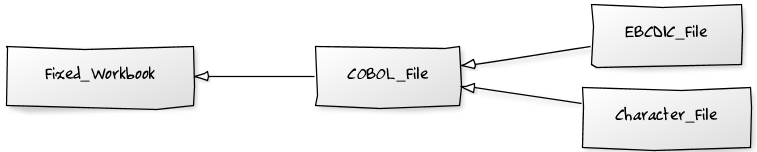
\includegraphics[width=6in]{cobol_file.png}


\subparagraph{COBOL File}
\label{cobol_init:cobol-file}\index{COBOL\_File (class in cobol)}

\begin{fulllineitems}
\phantomsection\label{cobol_init:cobol.COBOL_File}\pysigline{\strong{class }\code{cobol.}\bfcode{COBOL\_File}}
This class introduces the expanded version of \code{row\_get} that honors
a schema attribute with dimensionality.

\end{fulllineitems}


\begin{Verbatim}[commandchars=\\\{\}]
\PYG{k}{class} \PYG{n+nc}{COBOL\PYGZus{}File}\PYG{p}{(} \PYG{n}{Fixed\PYGZus{}Workbook} \PYG{p}{)}\PYG{p}{:}
    \PYG{l+s+sd}{\PYGZdq{}\PYGZdq{}\PYGZdq{}A COBOL \PYGZdq{}workbook\PYGZdq{} file which uses  :py:class:{}`cobol.RepeatingAttribute{}` and}
\PYG{l+s+sd}{    creates COBOL Cell values.  This is an abstraction which}
\PYG{l+s+sd}{    lacks specific decoding methods.}

\PYG{l+s+sd}{    This is a :py:class:{}`Fixed\PYGZus{}Workbook{}`: a file with fixed\PYGZhy{}sized, no\PYGZhy{}punctuation fields.}
\PYG{l+s+sd}{    A schema is required to parse the attributes.}

\PYG{l+s+sd}{    The rows are defined as :py:class:{}`cobol.ODO\PYGZus{}LazyRow{}` instances so that}
\PYG{l+s+sd}{    bad data can be gracefully skipped over and Occurs Depending On offsets}
\PYG{l+s+sd}{    can be properly calculated.}
\PYG{l+s+sd}{    \PYGZdq{}\PYGZdq{}\PYGZdq{}}
    \PYG{n}{row\PYGZus{}class}\PYG{o}{=} \PYG{n}{ODO\PYGZus{}LazyRow}
\end{Verbatim}
\index{row\_get\_index() (cobol.COBOL\_File method)}

\begin{fulllineitems}
\phantomsection\label{cobol_init:cobol.COBOL_File.row_get_index}\pysiglinewithargsret{\code{COBOL\_File.}\bfcode{row\_get\_index}}{\emph{row}, \emph{attr}, \emph{*index}}{}
Returning a particular Cell from a row, however, is more interesting for COBOL
because the Attribute may contains an ``OCCURS'' clause.  In which case, we may need
to assemble a tuple of values.

If there is dimensionality, then take the top-level dimension (\code{dim{[}0{]}}) and
use it as an iterator to fetch data based on the rest of the dimensions (\code{dim{[}1:{]}}).

This can assemble a recursive tuple-of-tuples if there are multiple levels
of dimensionality.

If too few index values are provided, a tuple of results is built around the missing values.

If enough values are provided, a single result object will be built.

\end{fulllineitems}


\begin{notice}{note}{Note:}
Performance

This is the most-used method. Removing the if-statement would be
a huge improvement.
\end{notice}

\begin{Verbatim}[commandchars=\\\{\}]
\PYG{k}{def} \PYG{n+nf}{row\PYGZus{}get\PYGZus{}index}\PYG{p}{(} \PYG{n+nb+bp}{self}\PYG{p}{,} \PYG{n}{row}\PYG{p}{,} \PYG{n}{attr}\PYG{p}{,} \PYG{o}{*}\PYG{n}{index} \PYG{p}{)}\PYG{p}{:}
    \PYG{l+s+sd}{\PYGZdq{}\PYGZdq{}\PYGZdq{}Emit a nested\PYGZhy{}tuple structure of Cell values using the given index values.}
\PYG{l+s+sd}{    :param row: the source Row.}
\PYG{l+s+sd}{    :param attr: the  :py:class:{}`cobol.RepeatingAttribute{}`}
\PYG{l+s+sd}{        with the original tuple of dimensions,}
\PYG{l+s+sd}{        or a :py:class:{}`cobol.IndexedAttribute{}` which has}
\PYG{l+s+sd}{        an offset and partial dimensions.}
\PYG{l+s+sd}{    :param index: optional tuple of index values to use.}
\PYG{l+s+sd}{        Instead of {}`{}`row\PYGZus{}get( schema.get(\PYGZsq{}name\PYGZsq{}).index(i) ){}`{}`}
\PYG{l+s+sd}{        we can use {}`{}`row\PYGZus{}get\PYGZus{}index( schema.get(\PYGZsq{}name\PYGZsq{}), i ){}`{}`}
\PYG{l+s+sd}{    :returns: a (possibly nested) tuple of Cell values matching the dims that lacked}
\PYG{l+s+sd}{        index values.}
\PYG{l+s+sd}{    \PYGZdq{}\PYGZdq{}\PYGZdq{}}
    \PYG{k}{if} \PYG{n}{attr}\PYG{o}{.}\PYG{n}{dimensionality} \PYG{o+ow}{and} \PYG{n}{index}\PYG{p}{:}
        \PYG{c}{\PYGZsh{} {}`{}`attr.index(){}`{}` probably not previously used.}
        \PYG{c}{\PYGZsh{} Apply all remaining values and get the resulting item.}
        \PYG{n}{final}\PYG{o}{=} \PYG{n}{attr}\PYG{o}{.}\PYG{n}{index}\PYG{p}{(} \PYG{o}{*}\PYG{n}{index} \PYG{p}{)}
        \PYG{k}{return} \PYG{n+nb+bp}{self}\PYG{o}{.}\PYG{n}{row\PYGZus{}get}\PYG{p}{(} \PYG{n}{row}\PYG{p}{,} \PYG{n}{final} \PYG{p}{)}
    \PYG{k}{elif} \PYG{n}{attr}\PYG{o}{.}\PYG{n}{dimensionality}\PYG{p}{:}
        \PYG{c}{\PYGZsh{} {}`{}`attr.index(){}`{}` previously used with partial arg values.}
        \PYG{c}{\PYGZsh{} Build composite result.}
        \PYG{n}{d}\PYG{o}{=} \PYG{n}{attr}\PYG{o}{.}\PYG{n}{dimensionality}\PYG{p}{[}\PYG{l+m+mi}{0}\PYG{p}{]}\PYG{o}{.}\PYG{n}{occurs}\PYG{o}{.}\PYG{n}{number}\PYG{p}{(}\PYG{n}{row}\PYG{p}{)}
        \PYG{n}{result}\PYG{o}{=} \PYG{p}{[}\PYG{p}{]}
        \PYG{k}{for} \PYG{n}{i} \PYG{o+ow}{in} \PYG{n+nb}{range}\PYG{p}{(}\PYG{n}{d}\PYG{p}{)}\PYG{p}{:}
            \PYG{n}{sub}\PYG{o}{=} \PYG{n}{attr}\PYG{o}{.}\PYG{n}{index}\PYG{p}{(}\PYG{n}{i}\PYG{p}{)}
            \PYG{n}{result}\PYG{o}{.}\PYG{n}{append}\PYG{p}{(} \PYG{n+nb+bp}{self}\PYG{o}{.}\PYG{n}{row\PYGZus{}get}\PYG{p}{(} \PYG{n}{row}\PYG{p}{,} \PYG{n}{sub} \PYG{p}{)} \PYG{p}{)}
        \PYG{k}{return} \PYG{n+nb}{tuple}\PYG{p}{(}\PYG{n}{result}\PYG{p}{)}
    \PYG{k}{else}\PYG{p}{:}
        \PYG{c}{\PYGZsh{} Doesn\PYGZsq{}t belong here, delegate.}
        \PYG{k}{return} \PYG{n+nb+bp}{self}\PYG{o}{.}\PYG{n}{row\PYGZus{}get}\PYG{p}{(} \PYG{n}{row}\PYG{p}{,} \PYG{n}{attr} \PYG{p}{)}
\end{Verbatim}
\index{row\_get() (cobol.COBOL\_File method)}

\begin{fulllineitems}
\phantomsection\label{cobol_init:cobol.COBOL_File.row_get}\pysiglinewithargsret{\code{COBOL\_File.}\bfcode{row\_get}}{\emph{row}, \emph{attr}}{}
The API method will get data from a row described by an attribute.
If the attribute has dimensions, then indices are used or multiple values are returned
by {\hyperref[cobol_init:cobol.COBOL_File.row_get_index]{\code{cobol.COBOL\_File.row\_get\_index()}}}.

If the attribute is has no dimensions, then it's simply pulled from the source row.

\end{fulllineitems}


\begin{notice}{note}{Note:}
Performance

This is the most-used method. Removing the if-statement would be
a huge improvement.
\end{notice}

\begin{Verbatim}[commandchars=\\\{\}]
\PYG{k}{def} \PYG{n+nf}{row\PYGZus{}get}\PYG{p}{(} \PYG{n+nb+bp}{self}\PYG{p}{,} \PYG{n}{row}\PYG{p}{,} \PYG{n}{attr} \PYG{p}{)}\PYG{p}{:}
    \PYG{l+s+sd}{\PYGZdq{}\PYGZdq{}\PYGZdq{}Create a Cell(s) from the row\PYGZsq{}s data.}
\PYG{l+s+sd}{    :param row: The current Row}
\PYG{l+s+sd}{    :param attr: The desired Attribute; possibly tweaked to}
\PYG{l+s+sd}{        have an offset and partial dimensions. Or possibly the original.}
\PYG{l+s+sd}{    :returns: A single Cell or a nested tuple of Cells if indexes}
\PYG{l+s+sd}{        were not provided.}
\PYG{l+s+sd}{    \PYGZdq{}\PYGZdq{}\PYGZdq{}}
    \PYG{k}{if} \PYG{n}{attr}\PYG{o}{.}\PYG{n}{dimensionality}\PYG{p}{:}
        \PYG{k}{return} \PYG{n+nb+bp}{self}\PYG{o}{.}\PYG{n}{row\PYGZus{}get\PYGZus{}index}\PYG{p}{(} \PYG{n}{row}\PYG{p}{,} \PYG{n}{attr} \PYG{p}{)}
    \PYG{k}{else}\PYG{p}{:}
        \PYG{n}{extract}\PYG{o}{=} \PYG{n}{row}\PYG{o}{.}\PYG{n}{\PYGZus{}state}\PYG{p}{[}\PYG{l+s}{\PYGZsq{}}\PYG{l+s}{data}\PYG{l+s}{\PYGZsq{}}\PYG{p}{]}\PYG{p}{[}\PYG{n}{attr}\PYG{o}{.}\PYG{n}{offset}\PYG{p}{:}\PYG{n}{attr}\PYG{o}{.}\PYG{n}{offset}\PYG{o}{+}\PYG{n}{attr}\PYG{o}{.}\PYG{n}{size}\PYG{p}{]}
        \PYG{k}{return} \PYG{n}{attr}\PYG{o}{.}\PYG{n}{create}\PYG{p}{(} \PYG{n}{extract}\PYG{p}{,} \PYG{n+nb+bp}{self}\PYG{p}{,} \PYG{n}{attr}\PYG{o}{=}\PYG{n}{attr} \PYG{p}{)}
\end{Verbatim}

Note that this depends on the superclass, which depends ordinary Unicode/ASCII line breaks.
This will not work for EBCDIC files, which may lack appropriate line break characters.
For that, we'll need to use specific physical format parsing helpers based on the
Z/OS RECFM parameter used to define the file.
\index{subrow() (cobol.COBOL\_File method)}

\begin{fulllineitems}
\phantomsection\label{cobol_init:cobol.COBOL_File.subrow}\pysiglinewithargsret{\code{COBOL\_File.}\bfcode{subrow}}{\emph{subschema}, \emph{text\_cell}}{}
In some COBOL files, there can be 01-level ``subrecords'' buried within an 01-level record.

We can use \code{wb.subrow(subschema, row.cell(schema\_header\_dict{[}'GENERIC-FIELD'{]}))}
to map a particular field (`GENERIC-FIELD') to an entire 01-level schema, creating
a ``subrow'' from a single field within the parent row.

\end{fulllineitems}


\begin{Verbatim}[commandchars=\\\{\}]
\PYG{k}{def} \PYG{n+nf}{subrow}\PYG{p}{(} \PYG{n+nb+bp}{self}\PYG{p}{,} \PYG{n}{subschema}\PYG{p}{,} \PYG{n}{text\PYGZus{}cell} \PYG{p}{)}\PYG{p}{:}
    \PYG{l+s+sd}{\PYGZdq{}\PYGZdq{}\PYGZdq{}Build a row\PYGZhy{}like object from a single field.}

\PYG{l+s+sd}{    :param subschema: a schema built from an 01\PYGZhy{}level DDE.}
\PYG{l+s+sd}{    :param text\PYGZus{}cell: a specific text cell to use.}
\PYG{l+s+sd}{    \PYGZdq{}\PYGZdq{}\PYGZdq{}}
    \PYG{n}{subrow} \PYG{o}{=} \PYG{n+nb+bp}{self}\PYG{o}{.}\PYG{n}{row\PYGZus{}class}\PYG{p}{(}
        \PYG{n}{stingray}\PYG{o}{.}\PYG{n}{sheet}\PYG{o}{.}\PYG{n}{ExternalSchemaSheet}\PYG{p}{(} \PYG{n+nb+bp}{self}\PYG{p}{,} \PYG{l+s}{\PYGZdq{}}\PYG{l+s}{\PYGZdq{}}\PYG{p}{,} \PYG{n}{subschema} \PYG{p}{)}\PYG{p}{,}
        \PYG{n}{data}\PYG{o}{=} \PYG{n}{text\PYGZus{}cell}\PYG{o}{.}\PYG{n}{raw}\PYG{p}{,}
    \PYG{p}{)}
    \PYG{k}{return} \PYG{n}{subrow}
\end{Verbatim}


\subparagraph{Character File}
\label{cobol_init:character-file}\index{Character\_File (class in cobol)}

\begin{fulllineitems}
\phantomsection\label{cobol_init:cobol.Character_File}\pysigline{\strong{class }\code{cobol.}\bfcode{Character\_File}}
This is subclass of {\hyperref[cobol_init:cobol.COBOL_File]{\code{COBOL\_File}}} that handles COBOL data parsing
where the underlying file is text. Since the file is text, Python handles
any OS-level bytes-to-text conversions.

\end{fulllineitems}


\begin{Verbatim}[commandchars=\\\{\}]
\PYG{k}{class} \PYG{n+nc}{Character\PYGZus{}File}\PYG{p}{(} \PYG{n}{COBOL\PYGZus{}File} \PYG{p}{)}\PYG{p}{:}
    \PYG{l+s+sd}{\PYGZdq{}\PYGZdq{}\PYGZdq{}A COBOL \PYGZdq{}workbook\PYGZdq{} file with decoding functions for}
\PYG{l+s+sd}{    proper character data.}
\PYG{l+s+sd}{    \PYGZdq{}\PYGZdq{}\PYGZdq{}}
\end{Verbatim}

The following functions are used to do data conversions for COBOL Character files.
Text is easy, Python's \code{io.open} has already handled this.

\begin{Verbatim}[commandchars=\\\{\}]
\PYG{n+nd}{@staticmethod}
\PYG{k}{def} \PYG{n+nf}{text}\PYG{p}{(} \PYG{n+nb}{buffer}\PYG{p}{,} \PYG{n}{attr} \PYG{p}{)}\PYG{p}{:}
    \PYG{l+s+sd}{\PYGZdq{}\PYGZdq{}\PYGZdq{}Extract a text field\PYGZsq{}s value.\PYGZdq{}\PYGZdq{}\PYGZdq{}}
    \PYG{k}{return} \PYG{n+nb}{buffer}
\end{Verbatim}

Numeric data with usage \code{DISPLAY} is essentially text. In some cases, the
picture has \code{V}, which means that we must handle this implicit decimal point.
The ``display'' feature is the COBOL default: everything is plain text.

Here's the core rule for character files:
\begin{itemize}
\item {} 
Leading separate sign is the default for character files.

\end{itemize}

COBOL can support other kinds of signs. This conversion doesn't.

\begin{Verbatim}[commandchars=\\\{\}]
\PYG{n+nd}{@staticmethod}
\PYG{k}{def} \PYG{n+nf}{number\PYGZus{}display}\PYG{p}{(} \PYG{n+nb}{buffer}\PYG{p}{,} \PYG{n}{attr} \PYG{p}{)}\PYG{p}{:}
    \PYG{l+s+sd}{\PYGZdq{}\PYGZdq{}\PYGZdq{}Extract a numeric field\PYGZsq{}s value.}
\PYG{l+s+sd}{    Based on leading, separate sign.}
\PYG{l+s+sd}{    \PYGZdq{}\PYGZdq{}\PYGZdq{}}
    \PYG{n}{final}\PYG{p}{,} \PYG{n}{alpha}\PYG{p}{,} \PYG{n}{length}\PYG{p}{,} \PYG{n}{scale}\PYG{p}{,} \PYG{n}{precision}\PYG{p}{,} \PYG{n}{signed}\PYG{p}{,} \PYG{n}{dec\PYGZus{}sign} \PYG{o}{=} \PYG{n}{attr}\PYG{o}{.}\PYG{n}{size\PYGZus{}scale\PYGZus{}precision}
    \PYG{k}{try}\PYG{p}{:}
        \PYG{n}{display}\PYG{o}{=}\PYG{n+nb}{buffer}\PYG{o}{.}\PYG{n}{strip}\PYG{p}{(}\PYG{p}{)}
        \PYG{k}{if} \PYG{n}{precision} \PYG{o}{!=} \PYG{l+m+mi}{0} \PYG{o+ow}{and} \PYG{n}{dec\PYGZus{}sign} \PYG{o}{==} \PYG{l+s}{\PYGZsq{}}\PYG{l+s}{V}\PYG{l+s}{\PYGZsq{}}\PYG{p}{:}
            \PYG{n}{display}\PYG{o}{=} \PYG{n}{display}\PYG{p}{[}\PYG{p}{:}\PYG{o}{\PYGZhy{}}\PYG{n}{precision}\PYG{p}{]}\PYG{o}{+}\PYG{l+s}{\PYGZdq{}}\PYG{l+s}{.}\PYG{l+s}{\PYGZdq{}}\PYG{o}{+}\PYG{n}{display}\PYG{p}{[}\PYG{o}{\PYGZhy{}}\PYG{n}{precision}\PYG{p}{:}\PYG{p}{]}
        \PYG{k}{return} \PYG{n}{decimal}\PYG{o}{.}\PYG{n}{Decimal}\PYG{p}{(} \PYG{n}{display} \PYG{p}{)}
    \PYG{k}{except} \PYG{n+ne}{Exception}\PYG{p}{:}
        \PYG{n}{Character\PYGZus{}File}\PYG{o}{.}\PYG{n}{log}\PYG{o}{.}\PYG{n}{debug}\PYG{p}{(} \PYG{l+s}{\PYGZdq{}}\PYG{l+s}{Can}\PYG{l+s}{\PYGZsq{}}\PYG{l+s}{t process \PYGZob{}0!r\PYGZcb{} from \PYGZob{}1!r\PYGZcb{}}\PYG{l+s}{\PYGZdq{}}\PYG{o}{.}\PYG{n}{format}\PYG{p}{(}\PYG{n}{display}\PYG{p}{,}\PYG{n+nb}{buffer}\PYG{p}{)} \PYG{p}{)}
        \PYG{k}{raise}
\end{Verbatim}

COMP-3 in proper character files may not make any sense at all.
A codec would make a hash of the bit patterns required.
However, we've defined the method here so that it can be used by the EBCDIC subclass
trivially.

We're going to build an ASCII version of the number by decoding the bytes into
a mutable bytearray and decorating them with decimal point and sign. This is
demonstrably faster and avoids object creation to the extent possible.

\begin{Verbatim}[commandchars=\\\{\}]
\PYG{n+nd}{@staticmethod}
\PYG{k}{def} \PYG{n+nf}{unpack}\PYG{p}{(} \PYG{n+nb}{buffer} \PYG{p}{)}\PYG{p}{:}
    \PYG{l+s+sd}{\PYGZdq{}\PYGZdq{}\PYGZdq{}Include \PYGZsq{} \PYGZsq{} position for leading sign character.}
\PYG{l+s+sd}{    Trailing sign field will be 48+0xd for negative.}
\PYG{l+s+sd}{    48+0xf is \PYGZdq{}unsigned\PYGZdq{} and 48+0xc is positive.}
\PYG{l+s+sd}{    \PYGZdq{}\PYGZdq{}\PYGZdq{}}
    \PYG{k}{yield} \PYG{l+m+mi}{32} \PYG{c}{\PYGZsh{} ord(b\PYGZsq{} \PYGZsq{})}
    \PYG{k}{for} \PYG{n}{n} \PYG{o+ow}{in} \PYG{n+nb}{buffer}\PYG{p}{:}
        \PYG{k}{yield} \PYG{l+m+mi}{48}\PYG{o}{+}\PYG{p}{(}\PYG{n}{n}\PYG{o}{\PYGZgt{}\PYGZgt{}}\PYG{l+m+mi}{4}\PYG{p}{)} \PYG{c}{\PYGZsh{} ord(b\PYGZsq{}0\PYGZsq{})}
        \PYG{k}{yield} \PYG{l+m+mi}{48}\PYG{o}{+}\PYG{p}{(}\PYG{n}{n}\PYG{o}{\PYGZam{}}\PYG{l+m+mh}{0x0f}\PYG{p}{)}

\PYG{n+nd}{@staticmethod}
\PYG{k}{def} \PYG{n+nf}{number\PYGZus{}comp3}\PYG{p}{(} \PYG{n+nb}{buffer}\PYG{p}{,} \PYG{n}{attr} \PYG{p}{)}\PYG{p}{:}
    \PYG{l+s+sd}{\PYGZdq{}\PYGZdq{}\PYGZdq{}Decode comp\PYGZhy{}3, packed decimal values.}

\PYG{l+s+sd}{    Each byte is two decimal digits.}

\PYG{l+s+sd}{    Last byte has a digit plus sign information: 0xd is \PYGZlt{}0, 0xf is unsigned, and 0xc \PYGZgt{}=0.}
\PYG{l+s+sd}{    \PYGZdq{}\PYGZdq{}\PYGZdq{}}
    \PYG{n}{final}\PYG{p}{,} \PYG{n}{alpha}\PYG{p}{,} \PYG{n}{length}\PYG{p}{,} \PYG{n}{scale}\PYG{p}{,} \PYG{n}{precision}\PYG{p}{,} \PYG{n}{signed}\PYG{p}{,} \PYG{n}{dec\PYGZus{}sign} \PYG{o}{=} \PYG{n}{attr}\PYG{o}{.}\PYG{n}{size\PYGZus{}scale\PYGZus{}precision}
    \PYG{c}{\PYGZsh{}print( repr(buffer), \PYGZdq{}from\PYGZdq{}, repr(display) )}
    \PYG{n}{digits} \PYG{o}{=} \PYG{n+nb}{bytearray}\PYG{p}{(} \PYG{n}{Character\PYGZus{}File}\PYG{o}{.}\PYG{n}{unpack}\PYG{p}{(} \PYG{n+nb}{buffer} \PYG{p}{)} \PYG{p}{)}
    \PYG{c}{\PYGZsh{} Proper sign in front; replace trailing sign with space.}
    \PYG{n}{digits}\PYG{p}{[}\PYG{l+m+mi}{0}\PYG{p}{]}\PYG{o}{=} \PYG{l+m+mi}{45} \PYG{k}{if} \PYG{n}{digits}\PYG{p}{[}\PYG{o}{\PYGZhy{}}\PYG{l+m+mi}{1}\PYG{p}{]}\PYG{o}{==}\PYG{l+m+mi}{48}\PYG{o}{+}\PYG{l+m+mh}{0xd} \PYG{k}{else} \PYG{l+m+mi}{32} \PYG{c}{\PYGZsh{} ord(b\PYGZsq{}\PYGZhy{}\PYGZsq{}), ord(b\PYGZsq{} \PYGZsq{})}
    \PYG{n}{digits}\PYG{p}{[}\PYG{o}{\PYGZhy{}}\PYG{l+m+mi}{1}\PYG{p}{]}\PYG{o}{=} \PYG{l+m+mi}{32} \PYG{c}{\PYGZsh{} ord(\PYGZsq{} \PYGZsq{})}
    \PYG{c}{\PYGZsh{} Add decimal place if needed.}
    \PYG{k}{if} \PYG{n}{precision}\PYG{p}{:}
        \PYG{n}{digits}\PYG{p}{[}\PYG{o}{\PYGZhy{}}\PYG{n}{precision}\PYG{p}{:}\PYG{p}{]}\PYG{o}{=} \PYG{n}{digits}\PYG{p}{[}\PYG{o}{\PYGZhy{}}\PYG{n}{precision}\PYG{o}{\PYGZhy{}}\PYG{l+m+mi}{1}\PYG{p}{:}\PYG{o}{\PYGZhy{}}\PYG{l+m+mi}{1}\PYG{p}{]} \PYG{c}{\PYGZsh{} Shift digits to right.}
        \PYG{n}{digits}\PYG{p}{[}\PYG{o}{\PYGZhy{}}\PYG{n}{precision}\PYG{o}{\PYGZhy{}}\PYG{l+m+mi}{1}\PYG{p}{]}\PYG{o}{=} \PYG{l+m+mi}{46} \PYG{c}{\PYGZsh{} Insert ord(b\PYGZsq{}.\PYGZsq{})}
    \PYG{k}{try}\PYG{p}{:}
        \PYG{k}{return} \PYG{n}{decimal}\PYG{o}{.}\PYG{n}{Decimal}\PYG{p}{(} \PYG{n}{digits}\PYG{o}{.}\PYG{n}{decode}\PYG{p}{(}\PYG{l+s}{\PYGZdq{}}\PYG{l+s}{ASCII}\PYG{l+s}{\PYGZdq{}}\PYG{p}{)} \PYG{p}{)}
    \PYG{k}{except} \PYG{n+ne}{Exception}\PYG{p}{:}
        \PYG{n}{Character\PYGZus{}File}\PYG{o}{.}\PYG{n}{log}\PYG{o}{.}\PYG{n}{debug}\PYG{p}{(} \PYG{l+s}{\PYGZdq{}}\PYG{l+s}{Can}\PYG{l+s}{\PYGZsq{}}\PYG{l+s}{t process \PYGZob{}0!r\PYGZcb{} from \PYGZob{}1!r\PYGZcb{}}\PYG{l+s}{\PYGZdq{}}\PYG{o}{.}\PYG{n}{format}\PYG{p}{(}\PYG{n}{digits}\PYG{p}{,}\PYG{n+nb}{buffer}\PYG{p}{)} \PYG{p}{)}
        \PYG{k}{raise}
\end{Verbatim}

COMP in proper character files may not make any sense, either.
A codec would make a hash of the bit patterns required.
Again, we've defined it here because that's relatively simple to extend.

We're simply going to unpack big-endian bytes.

\begin{Verbatim}[commandchars=\\\{\}]
\PYG{n+nd}{@staticmethod}
\PYG{k}{def} \PYG{n+nf}{number\PYGZus{}comp}\PYG{p}{(} \PYG{n+nb}{buffer}\PYG{p}{,} \PYG{n}{attr} \PYG{p}{)}\PYG{p}{:}
    \PYG{l+s+sd}{\PYGZdq{}\PYGZdq{}\PYGZdq{}Decode comp, binary values.\PYGZdq{}\PYGZdq{}\PYGZdq{}}
    \PYG{n}{final}\PYG{p}{,} \PYG{n}{alpha}\PYG{p}{,} \PYG{n}{length}\PYG{p}{,} \PYG{n}{scale}\PYG{p}{,} \PYG{n}{precision}\PYG{p}{,} \PYG{n}{signed}\PYG{p}{,} \PYG{n}{dec\PYGZus{}sign} \PYG{o}{=} \PYG{n}{attr}\PYG{o}{.}\PYG{n}{size\PYGZus{}scale\PYGZus{}precision}
    \PYG{k}{if} \PYG{n}{length} \PYG{o}{\PYGZlt{}}\PYG{o}{=} \PYG{l+m+mi}{4}\PYG{p}{:}
        \PYG{n}{sc}\PYG{p}{,} \PYG{n+nb}{bytes} \PYG{o}{=} \PYG{l+s}{\PYGZsq{}}\PYG{l+s}{\PYGZgt{}h}\PYG{l+s}{\PYGZsq{}}\PYG{p}{,} \PYG{l+m+mi}{2}
    \PYG{k}{elif} \PYG{n}{length} \PYG{o}{\PYGZlt{}}\PYG{o}{=} \PYG{l+m+mi}{9}\PYG{p}{:}
        \PYG{n}{sc}\PYG{p}{,} \PYG{n+nb}{bytes} \PYG{o}{=} \PYG{l+s}{\PYGZsq{}}\PYG{l+s}{\PYGZgt{}i}\PYG{l+s}{\PYGZsq{}}\PYG{p}{,} \PYG{l+m+mi}{4}
    \PYG{k}{else}\PYG{p}{:}
        \PYG{n}{sc}\PYG{p}{,} \PYG{n+nb}{bytes} \PYG{o}{=} \PYG{l+s}{\PYGZsq{}}\PYG{l+s}{\PYGZgt{}q}\PYG{l+s}{\PYGZsq{}}\PYG{p}{,} \PYG{l+m+mi}{8}
    \PYG{n}{n}\PYG{o}{=} \PYG{n}{struct}\PYG{o}{.}\PYG{n}{unpack}\PYG{p}{(} \PYG{n}{sc}\PYG{p}{,} \PYG{n+nb}{buffer} \PYG{p}{)}
    \PYG{k}{return} \PYG{n}{decimal}\PYG{o}{.}\PYG{n}{Decimal}\PYG{p}{(} \PYG{n}{n}\PYG{p}{[}\PYG{l+m+mi}{0}\PYG{p}{]} \PYG{p}{)}
\end{Verbatim}

Class-level logger

\begin{Verbatim}[commandchars=\\\{\}]
\PYG{n}{Character\PYGZus{}File}\PYG{o}{.}\PYG{n}{log}\PYG{o}{=} \PYG{n}{logging}\PYG{o}{.}\PYG{n}{getLogger}\PYG{p}{(} \PYG{n}{Character\PYGZus{}File}\PYG{o}{.}\PYG{n}{\PYGZus{}\PYGZus{}qualname\PYGZus{}\PYGZus{}} \PYG{p}{)}
\end{Verbatim}


\subparagraph{EBCDIC File}
\label{cobol_init:ebcdic-file}
The EBCDIC files require specific physical ``Record Format'' (RECFM) assistance.
These classes define a number of Z/OS RECFM conversion. We recognize four
actual RECFM's plus an additional special case.
\begin{itemize}
\item {} 
F - Fixed.

\item {} 
FB - Fixed Blocked.

\item {} 
V - Variable, data must have the RDW word preserved.

\item {} 
VB - Variable Blocked, data must have BDW and RDW words.

\item {} 
N - Variable, but no BDW or RDW words. This involves some buffer management
magic to recover the records properly.

\end{itemize}

\begin{notice}{note}{Note:}
IBM z/Architecture mainframes are all big-endian
\end{notice}
\index{RECFM\_Parser (class in cobol)}

\begin{fulllineitems}
\phantomsection\label{cobol_init:cobol.RECFM_Parser}\pysigline{\strong{class }\code{cobol.}\bfcode{RECFM\_Parser}}
This class hierarchy breaks up EBCDIC files into records.

\end{fulllineitems}


\begin{Verbatim}[commandchars=\\\{\}]
\PYG{k}{class} \PYG{n+nc}{RECFM\PYGZus{}Parser}\PYG{p}{:}
    \PYG{l+s+sd}{\PYGZdq{}\PYGZdq{}\PYGZdq{}Parse a physical file format.\PYGZdq{}\PYGZdq{}\PYGZdq{}}
    \PYG{k}{def} \PYG{n+nf}{record\PYGZus{}iter}\PYG{p}{(} \PYG{n+nb+bp}{self} \PYG{p}{)}\PYG{p}{:}
        \PYG{l+s+sd}{\PYGZdq{}\PYGZdq{}\PYGZdq{}Return each physical record, stripped of headers.\PYGZdq{}\PYGZdq{}\PYGZdq{}}
        \PYG{k}{raise} \PYG{n+ne}{NotImplementedError}
    \PYG{k}{def} \PYG{n+nf}{used}\PYG{p}{(} \PYG{n+nb+bp}{self}\PYG{p}{,} \PYG{n+nb}{bytes} \PYG{p}{)}\PYG{p}{:}
        \PYG{l+s+sd}{\PYGZdq{}\PYGZdq{}\PYGZdq{}The number of bytes actually consumed.}
\PYG{l+s+sd}{        Only really relevant for RECFM\PYGZus{}N subclass to handle variable\PYGZhy{}length}
\PYG{l+s+sd}{        records with no RDW/BDW overheads.}
\PYG{l+s+sd}{        \PYGZdq{}\PYGZdq{}\PYGZdq{}}
        \PYG{k}{pass}
\end{Verbatim}
\index{RECFM\_F (class in cobol)}

\begin{fulllineitems}
\phantomsection\label{cobol_init:cobol.RECFM_F}\pysigline{\strong{class }\code{cobol.}\bfcode{RECFM\_F}}
Simple fixed-length records. No header words.

\end{fulllineitems}


\begin{Verbatim}[commandchars=\\\{\}]
\PYG{k}{class} \PYG{n+nc}{RECFM\PYGZus{}F}\PYG{p}{(}\PYG{n}{RECFM\PYGZus{}Parser}\PYG{p}{)}\PYG{p}{:}
    \PYG{l+s+sd}{\PYGZdq{}\PYGZdq{}\PYGZdq{}Parse RECFM=F; the lrecl is the length of each record.\PYGZdq{}\PYGZdq{}\PYGZdq{}}
    \PYG{k}{def} \PYG{n+nf}{\PYGZus{}\PYGZus{}init\PYGZus{}\PYGZus{}}\PYG{p}{(} \PYG{n+nb+bp}{self}\PYG{p}{,} \PYG{n}{source}\PYG{p}{,} \PYG{n}{lrecl}\PYG{o}{=}\PYG{n+nb+bp}{None} \PYG{p}{)}\PYG{p}{:}
        \PYG{l+s+sd}{\PYGZdq{}\PYGZdq{}\PYGZdq{}}
\PYG{l+s+sd}{        :param source: the file}
\PYG{l+s+sd}{        :param lrecl: the record length.}
\PYG{l+s+sd}{        \PYGZdq{}\PYGZdq{}\PYGZdq{}}
        \PYG{n+nb}{super}\PYG{p}{(}\PYG{p}{)}\PYG{o}{.}\PYG{n}{\PYGZus{}\PYGZus{}init\PYGZus{}\PYGZus{}}\PYG{p}{(}\PYG{p}{)}
        \PYG{n+nb+bp}{self}\PYG{o}{.}\PYG{n}{source}\PYG{o}{=} \PYG{n}{source}
        \PYG{n+nb+bp}{self}\PYG{o}{.}\PYG{n}{lrecl}\PYG{o}{=} \PYG{n}{lrecl}
    \PYG{k}{def} \PYG{n+nf}{record\PYGZus{}iter}\PYG{p}{(} \PYG{n+nb+bp}{self} \PYG{p}{)}\PYG{p}{:}
        \PYG{n}{data}\PYG{o}{=} \PYG{n+nb+bp}{self}\PYG{o}{.}\PYG{n}{source}\PYG{o}{.}\PYG{n}{read}\PYG{p}{(}\PYG{n+nb+bp}{self}\PYG{o}{.}\PYG{n}{lrecl}\PYG{p}{)}
        \PYG{k}{while} \PYG{n+nb}{len}\PYG{p}{(}\PYG{n}{data}\PYG{p}{)} \PYG{o}{!=} \PYG{l+m+mi}{0}\PYG{p}{:}
            \PYG{k}{yield} \PYG{n}{data}
            \PYG{n}{data}\PYG{o}{=} \PYG{n+nb+bp}{self}\PYG{o}{.}\PYG{n}{source}\PYG{o}{.}\PYG{n}{read}\PYG{p}{(}\PYG{n+nb+bp}{self}\PYG{o}{.}\PYG{n}{lrecl}\PYG{p}{)}
    \PYG{k}{def} \PYG{n+nf}{rdw\PYGZus{}iter}\PYG{p}{(} \PYG{n+nb+bp}{self} \PYG{p}{)}\PYG{p}{:}
        \PYG{l+s+sd}{\PYGZdq{}\PYGZdq{}\PYGZdq{}Yield rows with RDW, effectively RECFM\PYGZus{}V format.\PYGZdq{}\PYGZdq{}\PYGZdq{}}
        \PYG{k}{for} \PYG{n}{row} \PYG{o+ow}{in} \PYG{n+nb+bp}{self}\PYG{o}{.}\PYG{n}{record\PYGZus{}iter}\PYG{p}{(}\PYG{p}{)}\PYG{p}{:}
            \PYG{k}{yield} \PYG{n}{struct}\PYG{o}{.}\PYG{n}{pack}\PYG{p}{(} \PYG{l+s}{\PYGZdq{}}\PYG{l+s}{\PYGZgt{}H2x}\PYG{l+s}{\PYGZdq{}}\PYG{p}{,} \PYG{n+nb}{len}\PYG{p}{(}\PYG{n}{row}\PYG{p}{)}\PYG{o}{+}\PYG{l+m+mi}{4} \PYG{p}{)}\PYG{o}{+}\PYG{n}{row}
\end{Verbatim}
\index{RECFM\_FB (class in cobol)}

\begin{fulllineitems}
\phantomsection\label{cobol_init:cobol.RECFM_FB}\pysigline{\strong{class }\code{cobol.}\bfcode{RECFM\_FB}}
Simple fixed-blocked records. No header words.

\end{fulllineitems}


\begin{Verbatim}[commandchars=\\\{\}]
\PYG{k}{class} \PYG{n+nc}{RECFM\PYGZus{}FB}\PYG{p}{(} \PYG{n}{RECFM\PYGZus{}F} \PYG{p}{)}\PYG{p}{:}
    \PYG{l+s+sd}{\PYGZdq{}\PYGZdq{}\PYGZdq{}Parse RECFM=FB; the lrecl is the length of each record.}

\PYG{l+s+sd}{    It\PYGZsq{}s not clear that there\PYGZsq{}s any difference between F and FB.}
\PYG{l+s+sd}{    \PYGZdq{}\PYGZdq{}\PYGZdq{}}
    \PYG{k}{pass}
\end{Verbatim}
\index{RECFM\_V (class in cobol)}

\begin{fulllineitems}
\phantomsection\label{cobol_init:cobol.RECFM_V}\pysigline{\strong{class }\code{cobol.}\bfcode{RECFM\_V}}
Variable-length records. Each record has an RDW header word with the length.

\end{fulllineitems}


\begin{Verbatim}[commandchars=\\\{\}]
\PYG{k}{class} \PYG{n+nc}{RECFM\PYGZus{}V}\PYG{p}{(}\PYG{n}{RECFM\PYGZus{}Parser}\PYG{p}{)}\PYG{p}{:}
    \PYG{l+s+sd}{\PYGZdq{}\PYGZdq{}\PYGZdq{}Parse RECFM=V; the lrecl is a maximum, which we ignore.\PYGZdq{}\PYGZdq{}\PYGZdq{}}
    \PYG{k}{def} \PYG{n+nf}{\PYGZus{}\PYGZus{}init\PYGZus{}\PYGZus{}}\PYG{p}{(} \PYG{n+nb+bp}{self}\PYG{p}{,} \PYG{n}{source}\PYG{p}{,} \PYG{n}{lrecl}\PYG{o}{=}\PYG{n+nb+bp}{None} \PYG{p}{)}\PYG{p}{:}
        \PYG{l+s+sd}{\PYGZdq{}\PYGZdq{}\PYGZdq{}}
\PYG{l+s+sd}{        :param source: the file}
\PYG{l+s+sd}{        :param lrecl: a maximum, but it\PYGZsq{}s ignored.}
\PYG{l+s+sd}{        \PYGZdq{}\PYGZdq{}\PYGZdq{}}
        \PYG{n+nb}{super}\PYG{p}{(}\PYG{p}{)}\PYG{o}{.}\PYG{n}{\PYGZus{}\PYGZus{}init\PYGZus{}\PYGZus{}}\PYG{p}{(}\PYG{p}{)}
        \PYG{n+nb+bp}{self}\PYG{o}{.}\PYG{n}{source}\PYG{o}{=} \PYG{n}{source}
    \PYG{k}{def} \PYG{n+nf}{record\PYGZus{}iter}\PYG{p}{(} \PYG{n+nb+bp}{self} \PYG{p}{)}\PYG{p}{:}
        \PYG{l+s+sd}{\PYGZdq{}\PYGZdq{}\PYGZdq{}Iterate over records, stripped of RDW\PYGZsq{}s.\PYGZdq{}\PYGZdq{}\PYGZdq{}}
        \PYG{k}{for} \PYG{n}{rdw}\PYG{p}{,} \PYG{n}{row} \PYG{o+ow}{in} \PYG{n+nb+bp}{self}\PYG{o}{.}\PYG{n}{\PYGZus{}data\PYGZus{}iter}\PYG{p}{(}\PYG{p}{)}\PYG{p}{:}
            \PYG{k}{yield} \PYG{n}{row}
    \PYG{k}{def} \PYG{n+nf}{rdw\PYGZus{}iter}\PYG{p}{(} \PYG{n+nb+bp}{self} \PYG{p}{)}\PYG{p}{:}
        \PYG{l+s+sd}{\PYGZdq{}\PYGZdq{}\PYGZdq{}Iterate over records which include the 4\PYGZhy{}byte RDW.\PYGZdq{}\PYGZdq{}\PYGZdq{}}
        \PYG{k}{for} \PYG{n}{rdw}\PYG{p}{,} \PYG{n}{row} \PYG{o+ow}{in} \PYG{n+nb+bp}{self}\PYG{o}{.}\PYG{n}{\PYGZus{}data\PYGZus{}iter}\PYG{p}{(}\PYG{p}{)}\PYG{p}{:}
            \PYG{k}{yield} \PYG{n}{rdw}\PYG{o}{+}\PYG{n}{row}
    \PYG{k}{def} \PYG{n+nf}{\PYGZus{}data\PYGZus{}iter}\PYG{p}{(} \PYG{n+nb+bp}{self} \PYG{p}{)}\PYG{p}{:}
        \PYG{n}{rdw}\PYG{o}{=} \PYG{n+nb+bp}{self}\PYG{o}{.}\PYG{n}{source}\PYG{o}{.}\PYG{n}{read}\PYG{p}{(}\PYG{l+m+mi}{4}\PYG{p}{)}
        \PYG{k}{while} \PYG{n+nb}{len}\PYG{p}{(}\PYG{n}{rdw}\PYG{p}{)} \PYG{o}{!=} \PYG{l+m+mi}{0}\PYG{p}{:}
            \PYG{n}{size} \PYG{o}{=} \PYG{n}{struct}\PYG{o}{.}\PYG{n}{unpack}\PYG{p}{(} \PYG{l+s}{\PYGZdq{}}\PYG{l+s}{\PYGZgt{}H2x}\PYG{l+s}{\PYGZdq{}}\PYG{p}{,} \PYG{n}{rdw} \PYG{p}{)}\PYG{p}{[}\PYG{l+m+mi}{0}\PYG{p}{]}
            \PYG{n}{data}\PYG{o}{=} \PYG{n+nb+bp}{self}\PYG{o}{.}\PYG{n}{source}\PYG{o}{.}\PYG{n}{read}\PYG{p}{(} \PYG{n}{size}\PYG{o}{\PYGZhy{}}\PYG{l+m+mi}{4} \PYG{p}{)}
            \PYG{k}{yield} \PYG{n}{rdw}\PYG{p}{,} \PYG{n}{data}
            \PYG{n}{rdw}\PYG{o}{=} \PYG{n+nb+bp}{self}\PYG{o}{.}\PYG{n}{source}\PYG{o}{.}\PYG{n}{read}\PYG{p}{(}\PYG{l+m+mi}{4}\PYG{p}{)}
\end{Verbatim}

We might want to implement the \code{RECFM\_Parser.used()} method to compare the number of bytes
used against the RDW size.
\index{RECFM\_VB (class in cobol)}

\begin{fulllineitems}
\phantomsection\label{cobol_init:cobol.RECFM_VB}\pysigline{\strong{class }\code{cobol.}\bfcode{RECFM\_VB}}
Variable-length, blocked records. Each block has a BDW; each record has an RDW header word.
These BDW and RDW describe the structure of the file.

\end{fulllineitems}


\begin{Verbatim}[commandchars=\\\{\}]
\PYG{k}{class} \PYG{n+nc}{RECFM\PYGZus{}VB}\PYG{p}{(}\PYG{n}{RECFM\PYGZus{}Parser}\PYG{p}{)}\PYG{p}{:}
    \PYG{l+s+sd}{\PYGZdq{}\PYGZdq{}\PYGZdq{}Parse RECFM=VB; the lrecl is a maximum, which we ignore.\PYGZdq{}\PYGZdq{}\PYGZdq{}}
    \PYG{k}{def} \PYG{n+nf}{\PYGZus{}\PYGZus{}init\PYGZus{}\PYGZus{}}\PYG{p}{(} \PYG{n+nb+bp}{self}\PYG{p}{,} \PYG{n}{source}\PYG{p}{,} \PYG{n}{lrecl}\PYG{o}{=}\PYG{n+nb+bp}{None} \PYG{p}{)}\PYG{p}{:}
        \PYG{l+s+sd}{\PYGZdq{}\PYGZdq{}\PYGZdq{}}
\PYG{l+s+sd}{        :param source: the file}
\PYG{l+s+sd}{        :param lrecl: a maximum, but it\PYGZsq{}s ignored.}
\PYG{l+s+sd}{        \PYGZdq{}\PYGZdq{}\PYGZdq{}}
        \PYG{n+nb}{super}\PYG{p}{(}\PYG{p}{)}\PYG{o}{.}\PYG{n}{\PYGZus{}\PYGZus{}init\PYGZus{}\PYGZus{}}\PYG{p}{(}\PYG{p}{)}
        \PYG{n+nb+bp}{self}\PYG{o}{.}\PYG{n}{source}\PYG{o}{=} \PYG{n}{source}
    \PYG{k}{def} \PYG{n+nf}{record\PYGZus{}iter}\PYG{p}{(} \PYG{n+nb+bp}{self} \PYG{p}{)}\PYG{p}{:}
        \PYG{l+s+sd}{\PYGZdq{}\PYGZdq{}\PYGZdq{}Iterate over records, stripped of RDW\PYGZsq{}s.\PYGZdq{}\PYGZdq{}\PYGZdq{}}
        \PYG{k}{for} \PYG{n}{rdw}\PYG{p}{,} \PYG{n}{row} \PYG{o+ow}{in} \PYG{n+nb+bp}{self}\PYG{o}{.}\PYG{n}{\PYGZus{}data\PYGZus{}iter}\PYG{p}{(}\PYG{p}{)}\PYG{p}{:}
            \PYG{k}{yield} \PYG{n}{row}
    \PYG{k}{def} \PYG{n+nf}{rdw\PYGZus{}iter}\PYG{p}{(} \PYG{n+nb+bp}{self} \PYG{p}{)}\PYG{p}{:}
        \PYG{l+s+sd}{\PYGZdq{}\PYGZdq{}\PYGZdq{}Iterate over records which include the 4\PYGZhy{}byte RDW.\PYGZdq{}\PYGZdq{}\PYGZdq{}}
        \PYG{k}{for} \PYG{n}{rdw}\PYG{p}{,} \PYG{n}{row} \PYG{o+ow}{in} \PYG{n+nb+bp}{self}\PYG{o}{.}\PYG{n}{\PYGZus{}data\PYGZus{}iter}\PYG{p}{(}\PYG{p}{)}\PYG{p}{:}
            \PYG{k}{yield} \PYG{n}{rdw}\PYG{o}{+}\PYG{n}{row}
    \PYG{k}{def} \PYG{n+nf}{bdw\PYGZus{}iter}\PYG{p}{(} \PYG{n+nb+bp}{self} \PYG{p}{)}\PYG{p}{:}
        \PYG{l+s+sd}{\PYGZdq{}\PYGZdq{}\PYGZdq{}Iterate over blocks, which include 4\PYGZhy{}byte BDW and records with 4\PYGZhy{}byte RDW\PYGZsq{}s.\PYGZdq{}\PYGZdq{}\PYGZdq{}}
        \PYG{n}{bdw}\PYG{o}{=} \PYG{n+nb+bp}{self}\PYG{o}{.}\PYG{n}{source}\PYG{o}{.}\PYG{n}{read}\PYG{p}{(}\PYG{l+m+mi}{4}\PYG{p}{)}
        \PYG{k}{while} \PYG{n+nb}{len}\PYG{p}{(}\PYG{n}{bdw}\PYG{p}{)} \PYG{o}{!=} \PYG{l+m+mi}{0}\PYG{p}{:}
            \PYG{n}{blksize} \PYG{o}{=} \PYG{n}{struct}\PYG{o}{.}\PYG{n}{unpack}\PYG{p}{(} \PYG{l+s}{\PYGZdq{}}\PYG{l+s}{\PYGZgt{}H2x}\PYG{l+s}{\PYGZdq{}}\PYG{p}{,} \PYG{n}{bdw} \PYG{p}{)}\PYG{p}{[}\PYG{l+m+mi}{0}\PYG{p}{]}
            \PYG{n}{block\PYGZus{}data}\PYG{o}{=} \PYG{n+nb+bp}{self}\PYG{o}{.}\PYG{n}{source}\PYG{o}{.}\PYG{n}{read}\PYG{p}{(} \PYG{n}{blksize}\PYG{o}{\PYGZhy{}}\PYG{l+m+mi}{4} \PYG{p}{)}
            \PYG{k}{yield} \PYG{n}{bdw}\PYG{o}{+}\PYG{n}{block\PYGZus{}data}
            \PYG{n}{bdw}\PYG{o}{=} \PYG{n+nb+bp}{self}\PYG{o}{.}\PYG{n}{source}\PYG{o}{.}\PYG{n}{read}\PYG{p}{(}\PYG{l+m+mi}{4}\PYG{p}{)}
    \PYG{k}{def} \PYG{n+nf}{\PYGZus{}data\PYGZus{}iter}\PYG{p}{(} \PYG{n+nb+bp}{self} \PYG{p}{)}\PYG{p}{:}
        \PYG{n}{bdw}\PYG{o}{=} \PYG{n+nb+bp}{self}\PYG{o}{.}\PYG{n}{source}\PYG{o}{.}\PYG{n}{read}\PYG{p}{(}\PYG{l+m+mi}{4}\PYG{p}{)}
        \PYG{k}{while} \PYG{n+nb}{len}\PYG{p}{(}\PYG{n}{bdw}\PYG{p}{)} \PYG{o}{!=} \PYG{l+m+mi}{0}\PYG{p}{:}
            \PYG{n}{blksize} \PYG{o}{=} \PYG{n}{struct}\PYG{o}{.}\PYG{n}{unpack}\PYG{p}{(} \PYG{l+s}{\PYGZdq{}}\PYG{l+s}{\PYGZgt{}H2x}\PYG{l+s}{\PYGZdq{}}\PYG{p}{,} \PYG{n}{bdw} \PYG{p}{)}\PYG{p}{[}\PYG{l+m+mi}{0}\PYG{p}{]}
            \PYG{n}{block\PYGZus{}data}\PYG{o}{=} \PYG{n+nb+bp}{self}\PYG{o}{.}\PYG{n}{source}\PYG{o}{.}\PYG{n}{read}\PYG{p}{(} \PYG{n}{blksize}\PYG{o}{\PYGZhy{}}\PYG{l+m+mi}{4} \PYG{p}{)}
            \PYG{n}{offset}\PYG{o}{=} \PYG{l+m+mi}{0}
            \PYG{k}{while} \PYG{n}{offset} \PYG{o}{!=} \PYG{n+nb}{len}\PYG{p}{(}\PYG{n}{block\PYGZus{}data}\PYG{p}{)}\PYG{p}{:}
                \PYG{k}{assert} \PYG{n}{offset}\PYG{o}{+}\PYG{l+m+mi}{4} \PYG{o}{\PYGZlt{}} \PYG{n+nb}{len}\PYG{p}{(}\PYG{n}{block\PYGZus{}data}\PYG{p}{)}\PYG{p}{,} \PYG{l+s}{\PYGZdq{}}\PYG{l+s}{Corrupted Data Block \PYGZob{}!r\PYGZcb{}}\PYG{l+s}{\PYGZdq{}}\PYG{o}{.}\PYG{n}{format}\PYG{p}{(}\PYG{n}{block\PYGZus{}data}\PYG{p}{)}
                \PYG{n}{rdw}\PYG{o}{=} \PYG{n}{block\PYGZus{}data}\PYG{p}{[}\PYG{n}{offset}\PYG{p}{:}\PYG{n}{offset}\PYG{o}{+}\PYG{l+m+mi}{4}\PYG{p}{]}
                \PYG{n}{size}\PYG{o}{=} \PYG{n}{struct}\PYG{o}{.}\PYG{n}{unpack}\PYG{p}{(} \PYG{l+s}{\PYGZdq{}}\PYG{l+s}{\PYGZgt{}H2x}\PYG{l+s}{\PYGZdq{}}\PYG{p}{,} \PYG{n}{rdw} \PYG{p}{)}\PYG{p}{[}\PYG{l+m+mi}{0}\PYG{p}{]}
                \PYG{k}{yield} \PYG{n}{rdw}\PYG{p}{,} \PYG{n}{block\PYGZus{}data}\PYG{p}{[}\PYG{n}{offset}\PYG{o}{+}\PYG{l+m+mi}{4}\PYG{p}{:}\PYG{n}{offset}\PYG{o}{+}\PYG{n}{size}\PYG{p}{]}
                \PYG{n}{offset} \PYG{o}{+}\PYG{o}{=} \PYG{n}{size}
            \PYG{n}{bdw}\PYG{o}{=} \PYG{n+nb+bp}{self}\PYG{o}{.}\PYG{n}{source}\PYG{o}{.}\PYG{n}{read}\PYG{p}{(}\PYG{l+m+mi}{4}\PYG{p}{)}
\end{Verbatim}

We might want to implement a generic \code{RECFM\_Parser.used()} method to compare the number of bytes
used against the RDW size and raise an exception in the event of a mismatch.
\index{RECFM\_N (class in cobol)}

\begin{fulllineitems}
\phantomsection\label{cobol_init:cobol.RECFM_N}\pysigline{\strong{class }\code{cobol.}\bfcode{RECFM\_N}}
Variable-length records without RDW's. Exasperating because we have to feed
bytes to the buffer as needed until the record is complete.

\end{fulllineitems}


\begin{Verbatim}[commandchars=\\\{\}]
\PYG{k}{class} \PYG{n+nc}{RECFM\PYGZus{}N}\PYG{p}{:}
    \PYG{l+s+sd}{\PYGZdq{}\PYGZdq{}\PYGZdq{}Parse RECFM=V without RDW (or RECFM=VB without BDW or RDW).}
\PYG{l+s+sd}{    The lrecl is ignored.}
\PYG{l+s+sd}{    \PYGZdq{}\PYGZdq{}\PYGZdq{}}
    \PYG{k}{def} \PYG{n+nf}{\PYGZus{}\PYGZus{}init\PYGZus{}\PYGZus{}}\PYG{p}{(} \PYG{n+nb+bp}{self}\PYG{p}{,} \PYG{n}{source}\PYG{p}{,} \PYG{n}{lrecl}\PYG{o}{=}\PYG{n+nb+bp}{None} \PYG{p}{)}\PYG{p}{:}
        \PYG{l+s+sd}{\PYGZdq{}\PYGZdq{}\PYGZdq{}}
\PYG{l+s+sd}{        :param source: the file}
\PYG{l+s+sd}{        :param lrecl: a maximum, but it\PYGZsq{}s ignored.}
\PYG{l+s+sd}{        \PYGZdq{}\PYGZdq{}\PYGZdq{}}
        \PYG{n+nb}{super}\PYG{p}{(}\PYG{p}{)}\PYG{o}{.}\PYG{n}{\PYGZus{}\PYGZus{}init\PYGZus{}\PYGZus{}}\PYG{p}{(}\PYG{p}{)}
        \PYG{n+nb+bp}{self}\PYG{o}{.}\PYG{n}{source}\PYG{o}{=} \PYG{n}{source}
        \PYG{n+nb+bp}{self}\PYG{o}{.}\PYG{n}{buffer}\PYG{o}{=} \PYG{n+nb+bp}{self}\PYG{o}{.}\PYG{n}{source}\PYG{o}{.}\PYG{n}{read}\PYG{p}{(} \PYG{l+m+mi}{32768} \PYG{p}{)}
    \PYG{k}{def} \PYG{n+nf}{record\PYGZus{}iter}\PYG{p}{(} \PYG{n+nb+bp}{self} \PYG{p}{)}\PYG{p}{:}
        \PYG{k}{while} \PYG{n+nb}{len}\PYG{p}{(}\PYG{n+nb+bp}{self}\PYG{o}{.}\PYG{n}{buffer}\PYG{p}{)} \PYG{o}{!=} \PYG{l+m+mi}{0}\PYG{p}{:}
            \PYG{k}{yield} \PYG{n+nb+bp}{self}\PYG{o}{.}\PYG{n}{buffer}
            \PYG{c}{\PYGZsh{} What if used() is not called? This will loop forever!}
    \PYG{k}{def} \PYG{n+nf}{used}\PYG{p}{(} \PYG{n+nb+bp}{self}\PYG{p}{,} \PYG{n+nb}{bytes} \PYG{p}{)}\PYG{p}{:}
        \PYG{c}{\PYGZsh{}print( \PYGZdq{}Consumed \PYGZob{}0\PYGZcb{} Bytes\PYGZdq{}.format(bytes) )}
        \PYG{n+nb+bp}{self}\PYG{o}{.}\PYG{n}{buffer}\PYG{o}{=} \PYG{n+nb+bp}{self}\PYG{o}{.}\PYG{n}{buffer}\PYG{p}{[}\PYG{n+nb}{bytes}\PYG{p}{:}\PYG{p}{]}\PYG{o}{+}\PYG{n+nb+bp}{self}\PYG{o}{.}\PYG{n}{source}\PYG{o}{.}\PYG{n}{read}\PYG{p}{(}\PYG{l+m+mi}{32768}\PYG{o}{\PYGZhy{}}\PYG{n+nb}{bytes}\PYG{p}{)}
\end{Verbatim}
\index{EBCDIC\_File (class in cobol)}

\begin{fulllineitems}
\phantomsection\label{cobol_init:cobol.EBCDIC_File}\pysigline{\strong{class }\code{cobol.}\bfcode{EBCDIC\_File}}
This subclass handles EBCDIC conversion and COMP-3
packed decimal numbers.  For this to work, the schema needs to use slightly different Cell-type conversions.

Otherwise, this is similar to processing simple character data.

\end{fulllineitems}


\begin{Verbatim}[commandchars=\\\{\}]
\PYG{k}{class} \PYG{n+nc}{EBCDIC\PYGZus{}File}\PYG{p}{(} \PYG{n}{Character\PYGZus{}File} \PYG{p}{)}\PYG{p}{:}
    \PYG{l+s+sd}{\PYGZdq{}\PYGZdq{}\PYGZdq{}A COBOL \PYGZdq{}workbook\PYGZdq{} file with decoding functions for}
\PYG{l+s+sd}{    EBCDIC data. If a file\PYGZus{}object is provided, it must be}
\PYG{l+s+sd}{    opened in byte mode, and no decoder can be used.}
\PYG{l+s+sd}{    \PYGZdq{}\PYGZdq{}\PYGZdq{}}
    \PYG{n}{decoder}\PYG{o}{=} \PYG{n}{codecs}\PYG{o}{.}\PYG{n}{getdecoder}\PYG{p}{(}\PYG{l+s}{\PYGZsq{}}\PYG{l+s}{cp037}\PYG{l+s}{\PYGZsq{}}\PYG{p}{)}
    \PYG{k}{def} \PYG{n+nf}{\PYGZus{}\PYGZus{}init\PYGZus{}\PYGZus{}}\PYG{p}{(} \PYG{n+nb+bp}{self}\PYG{p}{,} \PYG{n}{name}\PYG{p}{,} \PYG{n}{file\PYGZus{}object}\PYG{o}{=}\PYG{n+nb+bp}{None}\PYG{p}{,} \PYG{n}{schema}\PYG{o}{=}\PYG{n+nb+bp}{None}\PYG{p}{,} \PYG{n}{RECFM}\PYG{o}{=}\PYG{l+s}{\PYGZdq{}}\PYG{l+s}{N}\PYG{l+s}{\PYGZdq{}} \PYG{p}{)}\PYG{p}{:}
        \PYG{l+s+sd}{\PYGZdq{}\PYGZdq{}\PYGZdq{}Prepare the workbook for reading.}
\PYG{l+s+sd}{        :param name: File name}
\PYG{l+s+sd}{        :param file\PYGZus{}object: Optional file\PYGZhy{}like object.  If omitted, the named file is opened.}
\PYG{l+s+sd}{            The object must be opened in byte mode; no decoder should be used.}
\PYG{l+s+sd}{        :param schema: The schema to use.}
\PYG{l+s+sd}{        :param RECFM: The legacy Z/OS RECFM to use. This must be one}
\PYG{l+s+sd}{            of \PYGZdq{}F\PYGZdq{}, \PYGZdq{}FB\PYGZdq{}, \PYGZdq{}V\PYGZdq{}, \PYGZdq{}VB\PYGZdq{}. This is translated to an appropriate}
\PYG{l+s+sd}{            RECFM class: RECFM\PYGZus{}F, RECFM\PYGZus{}FB, RECFM\PYGZus{}V, or RECFM\PYGZus{}VB.}
\PYG{l+s+sd}{        \PYGZdq{}\PYGZdq{}\PYGZdq{}}
        \PYG{n+nb}{super}\PYG{p}{(}\PYG{p}{)}\PYG{o}{.}\PYG{n}{\PYGZus{}\PYGZus{}init\PYGZus{}\PYGZus{}}\PYG{p}{(} \PYG{n}{name}\PYG{p}{,} \PYG{n}{file\PYGZus{}object}\PYG{p}{,} \PYG{n}{schema} \PYG{p}{)}
        \PYG{k}{if} \PYG{n+nb+bp}{self}\PYG{o}{.}\PYG{n}{file\PYGZus{}obj}\PYG{p}{:}
            \PYG{n+nb+bp}{self}\PYG{o}{.}\PYG{n}{the\PYGZus{}file}\PYG{o}{=} \PYG{n+nb+bp}{None}
            \PYG{n+nb+bp}{self}\PYG{o}{.}\PYG{n}{wb}\PYG{o}{=} \PYG{n+nb+bp}{self}\PYG{o}{.}\PYG{n}{file\PYGZus{}obj}
        \PYG{k}{else}\PYG{p}{:}
            \PYG{n+nb+bp}{self}\PYG{o}{.}\PYG{n}{the\PYGZus{}file} \PYG{o}{=} \PYG{n+nb}{open}\PYG{p}{(} \PYG{n}{name}\PYG{p}{,} \PYG{l+s}{\PYGZsq{}}\PYG{l+s}{rb}\PYG{l+s}{\PYGZsq{}} \PYG{p}{)}
            \PYG{n+nb+bp}{self}\PYG{o}{.}\PYG{n}{wb}\PYG{o}{=} \PYG{n+nb+bp}{self}\PYG{o}{.}\PYG{n}{the\PYGZus{}file}
        \PYG{n+nb+bp}{self}\PYG{o}{.}\PYG{n}{schema}\PYG{o}{=} \PYG{n}{schema}
        \PYG{n}{parser\PYGZus{}class}\PYG{o}{=} \PYG{p}{\PYGZob{}}
            \PYG{l+s}{\PYGZdq{}}\PYG{l+s}{F}\PYG{l+s}{\PYGZdq{}} \PYG{p}{:} \PYG{n}{RECFM\PYGZus{}F}\PYG{p}{,}
            \PYG{l+s}{\PYGZdq{}}\PYG{l+s}{FB}\PYG{l+s}{\PYGZdq{}}\PYG{p}{:} \PYG{n}{RECFM\PYGZus{}FB}\PYG{p}{,}
            \PYG{l+s}{\PYGZdq{}}\PYG{l+s}{V}\PYG{l+s}{\PYGZdq{}} \PYG{p}{:} \PYG{n}{RECFM\PYGZus{}V}\PYG{p}{,}
            \PYG{l+s}{\PYGZdq{}}\PYG{l+s}{VB}\PYG{l+s}{\PYGZdq{}}\PYG{p}{:} \PYG{n}{RECFM\PYGZus{}VB}\PYG{p}{,}
            \PYG{l+s}{\PYGZdq{}}\PYG{l+s}{N}\PYG{l+s}{\PYGZdq{}}\PYG{p}{:}  \PYG{n}{RECFM\PYGZus{}N}\PYG{p}{,}
            \PYG{p}{\PYGZcb{}}\PYG{p}{[}\PYG{n}{RECFM}\PYG{p}{]}
        \PYG{n+nb+bp}{self}\PYG{o}{.}\PYG{n}{parser}\PYG{o}{=} \PYG{n}{parser\PYGZus{}class}\PYG{p}{(}\PYG{n+nb+bp}{self}\PYG{o}{.}\PYG{n}{wb}\PYG{p}{,} \PYG{n}{schema}\PYG{o}{.}\PYG{n}{lrecl}\PYG{p}{(}\PYG{p}{)}\PYG{p}{)}
\end{Verbatim}
\index{rows\_of() (cobol.EBCDIC\_File method)}

\begin{fulllineitems}
\phantomsection\label{cobol_init:cobol.EBCDIC_File.rows_of}\pysiglinewithargsret{\code{EBCDIC\_File.}\bfcode{rows\_of}}{\emph{sheet}}{}
We must extend the \code{workbook.Character\_File.rows\_of()} method to deal with
two issues:
\begin{itemize}
\item {} 
If the schema depends on a variably located DDE, then we need to do the
{\hyperref[cobol_defs:cobol.defs.setSizeAndOffset]{\code{cobol.defs.setSizeAndOffset()}}} function using the DDE.
This is done automagically by the {\hyperref[cobol_init:cobol.ODO_LazyRow]{\code{cobol.ODO\_LazyRow}}} object.

\item {} 
The legacy Z/OS RECFM details.
\begin{itemize}
\item {} 
We might have F or FB files, which are simply
long runs of EBCDIC bytes with no line breaks.
The LRECL must match the DDE.

\item {} 
We might have V (or VB) which have 4-byte header on each row (plus a 4-byte header on each block.)
The LRECL doesn't matter.

\item {} 
We can tolerate the awful situation where it's variable length (Occurs Depending On)
but there are no RECFM=V or RECFM=VB header words. We call this RECFM=N.
We fetch an oversized buffer and push back bytes beyond the end of the record.

\end{itemize}

This means that the \code{super().rows\_of( sheet )} has been replaced with a RECFM-aware
byte-parser. This byte parser may involve a back-and-forth to handle RECFM=N.
In the case of RECFM=N, we provide an overly-large buffer (32768 bytes) and after
any size and offset calculations, the \code{row.\_size} shows how many bytes were
actually used.

\end{itemize}

\end{fulllineitems}


\begin{Verbatim}[commandchars=\\\{\}]
\PYG{k}{def} \PYG{n+nf}{rows\PYGZus{}of}\PYG{p}{(} \PYG{n+nb+bp}{self}\PYG{p}{,} \PYG{n}{sheet} \PYG{p}{)}\PYG{p}{:}
    \PYG{l+s+sd}{\PYGZdq{}\PYGZdq{}\PYGZdq{}Iterate through all \PYGZdq{}rows\PYGZdq{} of this \PYGZdq{}sheet\PYGZdq{}.}
\PYG{l+s+sd}{    Really, this means all records of this COBOL file.}

\PYG{l+s+sd}{    Note the handshake with RECFM parser to show how many}
\PYG{l+s+sd}{    bytes were really needed.  For RECFM\PYGZus{}N, this is important.}
\PYG{l+s+sd}{    For other RECFM, this is ignored.}

\PYG{l+s+sd}{    :py:class:{}`cobol.ODO\PYGZus{}LazyRow{}` may adjust the schema}
\PYG{l+s+sd}{    if it has an Occurs Depending On.}
\PYG{l+s+sd}{    \PYGZdq{}\PYGZdq{}\PYGZdq{}}
    \PYG{k}{for} \PYG{n}{data} \PYG{o+ow}{in} \PYG{n+nb+bp}{self}\PYG{o}{.}\PYG{n}{parser}\PYG{o}{.}\PYG{n}{record\PYGZus{}iter}\PYG{p}{(}\PYG{p}{)}\PYG{p}{:}
        \PYG{n}{row}\PYG{o}{=} \PYG{n}{ODO\PYGZus{}LazyRow}\PYG{p}{(} \PYG{n}{sheet}\PYG{p}{,} \PYG{n}{data}\PYG{o}{=}\PYG{n}{data} \PYG{p}{)}
        \PYG{n+nb+bp}{self}\PYG{o}{.}\PYG{n}{parser}\PYG{o}{.}\PYG{n}{used}\PYG{p}{(}\PYG{n}{sheet}\PYG{o}{.}\PYG{n}{schema}\PYG{o}{.}\PYG{n}{lrecl}\PYG{p}{(}\PYG{p}{)}\PYG{p}{)}
        \PYG{k}{yield} \PYG{n}{row}
\end{Verbatim}

The following functions are used to do data conversions for COBOL EBCDIC files.
Text requires using a codec to translate EBCDIC-encoded characters.

\begin{Verbatim}[commandchars=\\\{\}]
\PYG{n+nd}{@staticmethod}
\PYG{k}{def} \PYG{n+nf}{text}\PYG{p}{(} \PYG{n+nb}{buffer}\PYG{p}{,} \PYG{n}{attr} \PYG{p}{)}\PYG{p}{:}
    \PYG{l+s+sd}{\PYGZdq{}\PYGZdq{}\PYGZdq{}Extract a text field\PYGZsq{}s value.\PYGZdq{}\PYGZdq{}\PYGZdq{}}
    \PYG{n}{text}\PYG{p}{,} \PYG{n}{size} \PYG{o}{=} \PYG{n}{EBCDIC\PYGZus{}File}\PYG{o}{.}\PYG{n}{decoder}\PYG{p}{(}\PYG{n+nb}{buffer}\PYG{p}{)}
    \PYG{k}{return} \PYG{n}{text}
\end{Verbatim}

When a number usage is \code{DISPLAY}, it's text:
we simply convert the bytes from EBCDIC to Unicode
and treat them more-or-less like a text field.

Note the subtlety around ``Signed'' display fields. The last byte
will include a sign in addition to the digit.
\begin{itemize}
\item {} 
The last EBCDIC character might be `xF1' to `xF9' which is unsigned.

\item {} 
The last EBCDIC character might be `xC1' to `xC9' which is positive.

\item {} 
The last EBCDIC character might be `xD1' to `xD9' which is negative.

\end{itemize}

Really.

\begin{Verbatim}[commandchars=\\\{\}]
\PYG{n+nd}{@staticmethod}
\PYG{k}{def} \PYG{n+nf}{number\PYGZus{}display}\PYG{p}{(} \PYG{n+nb}{buffer}\PYG{p}{,} \PYG{n}{attr} \PYG{p}{)}\PYG{p}{:}
    \PYG{l+s+sd}{\PYGZdq{}\PYGZdq{}\PYGZdq{}Extract a numeric field\PYGZsq{}s value.\PYGZdq{}\PYGZdq{}\PYGZdq{}}
    \PYG{k}{if} \PYG{n}{attr}\PYG{o}{.}\PYG{n}{size\PYGZus{}scale\PYGZus{}precision}\PYG{o}{.}\PYG{n}{signed}\PYG{p}{:}
        \PYG{c}{\PYGZsh{} Fiddle bits to make EBCDIC char from signed digit.}
        \PYG{n}{last\PYGZus{}digit} \PYG{o}{=} \PYG{n+nb}{bytes}\PYG{p}{(} \PYG{p}{[}\PYG{p}{(}\PYG{n+nb}{buffer}\PYG{p}{[}\PYG{o}{\PYGZhy{}}\PYG{l+m+mi}{1}\PYG{p}{]} \PYG{o}{\PYGZam{}} \PYG{l+m+mh}{0x0F}\PYG{p}{)} \PYG{o}{\textbar{}} \PYG{l+m+mh}{0xF0}\PYG{p}{]} \PYG{p}{)}
        \PYG{n}{sign} \PYG{o}{=} \PYG{l+s}{\PYGZsq{}}\PYG{l+s}{\PYGZhy{}}\PYG{l+s}{\PYGZsq{}} \PYG{k}{if} \PYG{n+nb}{buffer}\PYG{p}{[}\PYG{o}{\PYGZhy{}}\PYG{l+m+mi}{1}\PYG{p}{]} \PYG{o}{\PYGZgt{}\PYGZgt{}} \PYG{l+m+mi}{4} \PYG{o}{==} \PYG{l+m+mh}{0xD} \PYG{k}{else} \PYG{l+s}{\PYGZsq{}}\PYG{l+s}{\PYGZsq{}}
        \PYG{n}{text}\PYG{p}{,} \PYG{n}{size} \PYG{o}{=} \PYG{n}{EBCDIC\PYGZus{}File}\PYG{o}{.}\PYG{n}{decoder}\PYG{p}{(}\PYG{n}{last\PYGZus{}digit} \PYG{k}{if} \PYG{n+nb}{len}\PYG{p}{(}\PYG{n+nb}{buffer}\PYG{p}{)} \PYG{o}{==} \PYG{l+m+mi}{1} \PYG{k}{else} \PYG{n+nb}{buffer}\PYG{p}{[}\PYG{p}{:}\PYG{o}{\PYGZhy{}}\PYG{l+m+mi}{1}\PYG{p}{]} \PYG{o}{+} \PYG{n}{last\PYGZus{}digit}\PYG{p}{)}
        \PYG{k}{return} \PYG{n}{Character\PYGZus{}File}\PYG{o}{.}\PYG{n}{number\PYGZus{}display}\PYG{p}{(} \PYG{n}{sign}\PYG{o}{+}\PYG{n}{text}\PYG{p}{,} \PYG{n}{attr} \PYG{p}{)}
    \PYG{k}{else}\PYG{p}{:}
        \PYG{n}{text}\PYG{p}{,} \PYG{n}{size} \PYG{o}{=} \PYG{n}{EBCDIC\PYGZus{}File}\PYG{o}{.}\PYG{n}{decoder}\PYG{p}{(}\PYG{n+nb}{buffer}\PYG{p}{)}
        \PYG{k}{return} \PYG{n}{Character\PYGZus{}File}\PYG{o}{.}\PYG{n}{number\PYGZus{}display}\PYG{p}{(} \PYG{n}{text}\PYG{p}{,} \PYG{n}{attr} \PYG{p}{)}
\end{Verbatim}


\subparagraph{ASCII File}
\label{cobol_init:ascii-file}
We could define a subclass for files encoded in ASCII which contain COMP and COMP-3 values.

This is left as a future extension.


\subsubsection{COBOL Loader Module -- Parse COBOL Source to Load a Schema}
\label{cobol_loader:cobol-loader}\label{cobol_loader:cobol-loader-module-parse-cobol-source-to-load-a-schema}\label{cobol_loader::doc}\label{cobol_loader:module-cobol.loader}\index{cobol.loader (module)}
Parsing a spreadsheet schema is relatively easy: see {\hyperref[schema_loader:schema-loader]{\emph{Schema Loader Module -- Load Embedded or External Schema}}}.
Parsing a COBOL schema, however, is a bit more complex. We need to parse
COBOL sources code to decode Data Definition Elements (DDE's) and create
a usable representation of the DDE that matches the Stingray schema model.

We'll wind up with two representations of the COBOL schema:
\begin{itemize}
\item {} 
The original DDE hierarchy. See {\hyperref[cobol_loader:dde-loader-design]{DDE Loader Design}} for details.

\item {} 
A flattened version that's a  {\hyperref[schema:schema.Schema]{\code{schema.Schema}}} instance.

\end{itemize}

A new {\hyperref[schema_loader:schema.loader.ExternalSchemaLoader]{\code{schema.loader.ExternalSchemaLoader}}} subclass is required
to parse the DDE sublanguage of COBOL.  The {\hyperref[cobol_loader:cobol-schema-loader-class]{COBOL Schema Loader Class}} section
details this. A loader will build the hierarchical
DDE from the COBOL source, decorate this with size and offset information,
then flatten it into a simple {\hyperref[schema:schema.Schema]{\code{schema.Schema}}} instance.


\paragraph{Load A Schema Use Case}
\label{cobol_loader:load-a-schema-use-case}
The goal of use case is to load a schema encoded in COBOL.  This breaks down
into two steps.
\begin{enumerate}
\item {} 
Parse the COBOL ``copybook'' source file.

\item {} 
Produce a {\hyperref[schema:schema.Schema]{\code{schema.Schema}}} instance that can be used to access data
in a COBOL file.

\end{enumerate}

Ideally, this will look something like the following.

\begin{Verbatim}[commandchars=\\\{\}]
\PYG{k}{with} \PYG{n+nb}{open}\PYG{p}{(}\PYG{l+s}{\PYGZdq{}}\PYG{l+s}{sample/zipcty.cob}\PYG{l+s}{\PYGZdq{}}\PYG{p}{,} \PYG{l+s}{\PYGZdq{}}\PYG{l+s}{r}\PYG{l+s}{\PYGZdq{}}\PYG{p}{)} \PYG{k}{as} \PYG{n}{cobol}\PYG{p}{:}
    \PYG{n}{schema}\PYG{o}{=} \PYG{n}{stingray}\PYG{o}{.}\PYG{n}{cobol}\PYG{o}{.}\PYG{n}{loader}\PYG{o}{.}\PYG{n}{COBOLSchemaLoader}\PYG{p}{(} \PYG{n}{cobol} \PYG{p}{)}\PYG{o}{.}\PYG{n}{load}\PYG{p}{(}\PYG{p}{)}
    \PYG{c}{\PYGZsh{}pprint.pprint( schema )}
\PYG{k}{for} \PYG{n}{filename} \PYG{o+ow}{in} \PYG{l+s}{\PYGZsq{}}\PYG{l+s}{sample/zipcty1}\PYG{l+s}{\PYGZsq{}}\PYG{p}{,} \PYG{l+s}{\PYGZsq{}}\PYG{l+s}{sample/zipcty2}\PYG{l+s}{\PYGZsq{}}\PYG{p}{:}
    \PYG{k}{with} \PYG{n}{stingray}\PYG{o}{.}\PYG{n}{cobol}\PYG{o}{.}\PYG{n}{Character\PYGZus{}File}\PYG{p}{(} \PYG{n}{filename}\PYG{p}{,} \PYG{n}{schema}\PYG{o}{=}\PYG{n}{schema} \PYG{p}{)} \PYG{k}{as} \PYG{n}{wb}\PYG{p}{:}
        \PYG{n}{sheet}\PYG{o}{=} \PYG{n}{wb}\PYG{o}{.}\PYG{n}{sheet}\PYG{p}{(} \PYG{n}{filename} \PYG{p}{)}
        \PYG{n}{counts}\PYG{o}{=} \PYG{n}{process\PYGZus{}sheet}\PYG{p}{(} \PYG{n}{sheet} \PYG{p}{)}
        \PYG{n}{pprint}\PYG{o}{.}\PYG{n}{pprint}\PYG{p}{(} \PYG{n}{counts} \PYG{p}{)}
\end{Verbatim}

Step 1 is to open the COBOL DDE ``copybook'' file, \code{zipcty.cob} that defines the layout.
We build the schema using a {\hyperref[cobol_loader:cobol.loader.COBOLSchemaLoader]{\code{cobol.loader.COBOLSchemaLoader}}}.

Step 2 is to open the source data, \code{zipcty1} with the data.
We've made a {\hyperref[sheet:sheet.Sheet]{\code{sheet.Sheet}}} from the file: the sheet's name is \code{"zipcty1"},
the the schema is the external provided when we opened the {\hyperref[cobol_init:cobol.Character_File]{\code{cobol.Character\_File}}}.

Once the sheet is available, we can then run some function, \code{process\_sheet}, on the
sheet. This will use the {\hyperref[sheet:sheet.Sheet]{\code{sheet.Sheet}}} API to process rows and cells of the
sheet. Each piece of source data is loaded as a kind of {\hyperref[cell:cell.Cell]{\code{cell.Cell}}}.

We can then use appropriate conversions to recover Python objects.
This leads us to the second use case.

Here's what a \code{process\_sheet()} function might look like in this context.

\begin{Verbatim}[commandchars=\\\{\}]
\PYG{k}{def} \PYG{n+nf}{process\PYGZus{}sheet}\PYG{p}{(} \PYG{n}{sheet} \PYG{p}{)}\PYG{p}{:}
    \PYG{n}{schema\PYGZus{}dict}\PYG{o}{=} \PYG{n+nb}{dict}\PYG{p}{(} \PYG{p}{(}\PYG{n}{a}\PYG{o}{.}\PYG{n}{name}\PYG{p}{,} \PYG{n}{a}\PYG{p}{)} \PYG{k}{for} \PYG{n}{a} \PYG{o+ow}{in} \PYG{n}{sheet}\PYG{o}{.}\PYG{n}{schema} \PYG{p}{)}
    \PYG{n}{schema\PYGZus{}dict}\PYG{o}{.}\PYG{n}{update}\PYG{p}{(} \PYG{n+nb}{dict}\PYG{p}{(} \PYG{p}{(}\PYG{n}{a}\PYG{o}{.}\PYG{n}{path}\PYG{p}{,} \PYG{n}{a}\PYG{p}{)} \PYG{k}{for} \PYG{n}{a} \PYG{o+ow}{in} \PYG{n}{sheet}\PYG{o}{.}\PYG{n}{schema} \PYG{p}{)} \PYG{p}{)}

    \PYG{n}{counts}\PYG{o}{=} \PYG{p}{\PYGZob{}} \PYG{l+s}{\PYGZsq{}}\PYG{l+s}{read}\PYG{l+s}{\PYGZsq{}}\PYG{p}{:} \PYG{l+m+mi}{0} \PYG{p}{\PYGZcb{}}

    \PYG{n}{row\PYGZus{}iter}\PYG{o}{=} \PYG{n}{sheet}\PYG{o}{.}\PYG{n}{rows}\PYG{p}{(}\PYG{p}{)}
    \PYG{n}{header}\PYG{o}{=} \PYG{n}{header\PYGZus{}builder}\PYG{p}{(} \PYG{n+nb}{next}\PYG{p}{(}\PYG{n}{row\PYGZus{}iter}\PYG{p}{)}\PYG{p}{,} \PYG{n}{schema\PYGZus{}dict} \PYG{p}{)}
    \PYG{k}{print}\PYG{p}{(} \PYG{n}{header} \PYG{p}{)}
    \PYG{k}{for} \PYG{n}{row} \PYG{o+ow}{in} \PYG{n}{row\PYGZus{}iter}\PYG{p}{:}
        \PYG{n}{detail}\PYG{o}{=} \PYG{n}{row\PYGZus{}builder}\PYG{p}{(} \PYG{n}{row}\PYG{p}{,} \PYG{n}{schema\PYGZus{}dict} \PYG{p}{)}
        \PYG{k}{print}\PYG{p}{(} \PYG{n}{detail} \PYG{p}{)}
        \PYG{n}{counts}\PYG{p}{[}\PYG{l+s}{\PYGZsq{}}\PYG{l+s}{read}\PYG{l+s}{\PYGZsq{}}\PYG{p}{]} \PYG{o}{+}\PYG{o}{=} \PYG{l+m+mi}{1}
    \PYG{k}{return} \PYG{n}{counts}
\end{Verbatim}

First, we've build two versions of the schema, indexed by low-level item name
and the full path to an item. In some cases, the low-level DDE items are unique,
and the paths are not required. In other cases, the paths are required.

We've initialized some record counts, always a good practice.

We've fetched the first record and used some function named \code{header\_builder()} to
transform the record into a header, which we print.

We've fetched all other records and used a function named \code{row\_builder()} to
transform every following record into details, which we also print.

This shows a physical head-tail processing. In some cases, there's an attribute
which differentiates headers, body and trailers.


\paragraph{Use A Schema Use Case}
\label{cobol_loader:use-a-schema-use-case}
The goal of this use case is to build usable Python objects from the source file data.

For each row, there's a two-step operation.
\begin{enumerate}
\item {} 
Access elements of each row using the COBOL DDE structure.

\item {} 
Build Python objects from the Cells found in the row.

\end{enumerate}

Generally, we must use lazy evaluation as shown in this example:

\begin{Verbatim}[commandchars=\\\{\}]
\PYG{k}{def} \PYG{n+nf}{header\PYGZus{}builder}\PYG{p}{(}\PYG{n}{row}\PYG{p}{,} \PYG{n}{schema}\PYG{p}{)}\PYG{p}{:}
    \PYG{k}{return} \PYG{n+nb}{dict}\PYG{p}{(}
        \PYG{n}{file\PYGZus{}version\PYGZus{}year}\PYG{o}{=} \PYG{n}{row}\PYG{o}{.}\PYG{n}{cell}\PYG{p}{(}\PYG{n}{schema}\PYG{p}{[}\PYG{l+s}{\PYGZsq{}}\PYG{l+s}{FILE\PYGZhy{}VERSION\PYGZhy{}YEAR}\PYG{l+s}{\PYGZsq{}}\PYG{p}{]}\PYG{p}{)}\PYG{o}{.}\PYG{n}{to\PYGZus{}str}\PYG{p}{(}\PYG{p}{)}\PYG{p}{,}
        \PYG{n}{file\PYGZus{}version\PYGZus{}month}\PYG{o}{=} \PYG{n}{row}\PYG{o}{.}\PYG{n}{cell}\PYG{p}{(}\PYG{n}{schema}\PYG{p}{[}\PYG{l+s}{\PYGZsq{}}\PYG{l+s}{FILE\PYGZhy{}VERSION\PYGZhy{}MONTH}\PYG{l+s}{\PYGZsq{}}\PYG{p}{]}\PYG{p}{)}\PYG{o}{.}\PYG{n}{to\PYGZus{}str}\PYG{p}{(}\PYG{p}{)}\PYG{p}{,}
        \PYG{n}{copyright\PYGZus{}symbol}\PYG{o}{=} \PYG{n}{row}\PYG{o}{.}\PYG{n}{cell}\PYG{p}{(}\PYG{n}{schema}\PYG{p}{[}\PYG{l+s}{\PYGZsq{}}\PYG{l+s}{COPYRIGHT\PYGZhy{}SYMBOL}\PYG{l+s}{\PYGZsq{}}\PYG{p}{]}\PYG{p}{)}\PYG{o}{.}\PYG{n}{to\PYGZus{}str}\PYG{p}{(}\PYG{p}{)}\PYG{p}{,}
        \PYG{n}{tape\PYGZus{}sequence\PYGZus{}no}\PYG{o}{=} \PYG{n}{row}\PYG{o}{.}\PYG{n}{cell}\PYG{p}{(}\PYG{n}{schema}\PYG{p}{[}\PYG{l+s}{\PYGZsq{}}\PYG{l+s}{TAPE\PYGZhy{}SEQUENCE\PYGZhy{}NO}\PYG{l+s}{\PYGZsq{}}\PYG{p}{]}\PYG{p}{)}\PYG{o}{.}\PYG{n}{to\PYGZus{}str}\PYG{p}{(}\PYG{p}{)}\PYG{p}{,}
    \PYG{p}{)}

\PYG{k}{def} \PYG{n+nf}{row\PYGZus{}builder}\PYG{p}{(}\PYG{n}{row}\PYG{p}{,} \PYG{n}{schema}\PYG{p}{)}\PYG{p}{:}
    \PYG{k}{return} \PYG{n+nb}{dict}\PYG{p}{(}
        \PYG{n}{zip\PYGZus{}code}\PYG{o}{=} \PYG{n}{row}\PYG{o}{.}\PYG{n}{cell}\PYG{p}{(}\PYG{n}{schema}\PYG{p}{[}\PYG{l+s}{\PYGZsq{}}\PYG{l+s}{ZIP\PYGZhy{}CODE}\PYG{l+s}{\PYGZsq{}}\PYG{p}{]}\PYG{p}{)}\PYG{o}{.}\PYG{n}{to\PYGZus{}str}\PYG{p}{(}\PYG{p}{)}\PYG{p}{,}
        \PYG{n}{update\PYGZus{}key\PYGZus{}no}\PYG{o}{=} \PYG{n}{row}\PYG{o}{.}\PYG{n}{cell}\PYG{p}{(}\PYG{n}{schema}\PYG{p}{[}\PYG{l+s}{\PYGZsq{}}\PYG{l+s}{UPDATE\PYGZhy{}KEY\PYGZhy{}NO}\PYG{l+s}{\PYGZsq{}}\PYG{p}{]}\PYG{p}{)}\PYG{o}{.}\PYG{n}{to\PYGZus{}str}\PYG{p}{(}\PYG{p}{)}\PYG{p}{,}
        \PYG{n}{low\PYGZus{}sector}\PYG{o}{=} \PYG{n}{row}\PYG{o}{.}\PYG{n}{cell}\PYG{p}{(}\PYG{n}{schema}\PYG{p}{[}\PYG{l+s}{\PYGZsq{}}\PYG{l+s}{COUNTY\PYGZhy{}CROSS\PYGZhy{}REFERENCE\PYGZhy{}RECORD.ZIP\PYGZhy{}ADD\PYGZhy{}ON\PYGZhy{}RANGE.ZIP\PYGZhy{}ADD\PYGZhy{}ON\PYGZhy{}LOW\PYGZhy{}NO.ZIP\PYGZhy{}SECTOR\PYGZhy{}NO}\PYG{l+s}{\PYGZsq{}}\PYG{p}{]}\PYG{p}{)}\PYG{o}{.}\PYG{n}{to\PYGZus{}str}\PYG{p}{(}\PYG{p}{)}\PYG{p}{,}
        \PYG{n}{low\PYGZus{}segment}\PYG{o}{=} \PYG{n}{row}\PYG{o}{.}\PYG{n}{cell}\PYG{p}{(}\PYG{n}{schema}\PYG{p}{[}\PYG{l+s}{\PYGZsq{}}\PYG{l+s}{COUNTY\PYGZhy{}CROSS\PYGZhy{}REFERENCE\PYGZhy{}RECORD.ZIP\PYGZhy{}ADD\PYGZhy{}ON\PYGZhy{}RANGE.ZIP\PYGZhy{}ADD\PYGZhy{}ON\PYGZhy{}LOW\PYGZhy{}NO.ZIP\PYGZhy{}SEGMENT\PYGZhy{}NO}\PYG{l+s}{\PYGZsq{}}\PYG{p}{]}\PYG{p}{)}\PYG{o}{.}\PYG{n}{to\PYGZus{}str}\PYG{p}{(}\PYG{p}{)}\PYG{p}{,}
        \PYG{n}{high\PYGZus{}sector}\PYG{o}{=} \PYG{n}{row}\PYG{o}{.}\PYG{n}{cell}\PYG{p}{(}\PYG{n}{schema}\PYG{p}{[}\PYG{l+s}{\PYGZsq{}}\PYG{l+s}{COUNTY\PYGZhy{}CROSS\PYGZhy{}REFERENCE\PYGZhy{}RECORD.ZIP\PYGZhy{}ADD\PYGZhy{}ON\PYGZhy{}RANGE.ZIP\PYGZhy{}ADD\PYGZhy{}ON\PYGZhy{}HIGH\PYGZhy{}NO.ZIP\PYGZhy{}SECTOR\PYGZhy{}NO}\PYG{l+s}{\PYGZsq{}}\PYG{p}{]}\PYG{p}{)}\PYG{o}{.}\PYG{n}{to\PYGZus{}str}\PYG{p}{(}\PYG{p}{)}\PYG{p}{,}
        \PYG{n}{high\PYGZus{}segment}\PYG{o}{=} \PYG{n}{row}\PYG{o}{.}\PYG{n}{cell}\PYG{p}{(}\PYG{n}{schema}\PYG{p}{[}\PYG{l+s}{\PYGZsq{}}\PYG{l+s}{COUNTY\PYGZhy{}CROSS\PYGZhy{}REFERENCE\PYGZhy{}RECORD.ZIP\PYGZhy{}ADD\PYGZhy{}ON\PYGZhy{}RANGE.ZIP\PYGZhy{}ADD\PYGZhy{}ON\PYGZhy{}HIGH\PYGZhy{}NO.ZIP\PYGZhy{}SEGMENT\PYGZhy{}NO}\PYG{l+s}{\PYGZsq{}}\PYG{p}{]}\PYG{p}{)}\PYG{o}{.}\PYG{n}{to\PYGZus{}str}\PYG{p}{(}\PYG{p}{)}\PYG{p}{,}
        \PYG{n}{state\PYGZus{}abbrev}\PYG{o}{=} \PYG{n}{row}\PYG{o}{.}\PYG{n}{cell}\PYG{p}{(}\PYG{n}{schema}\PYG{p}{[}\PYG{l+s}{\PYGZsq{}}\PYG{l+s}{STATE\PYGZhy{}ABBREV}\PYG{l+s}{\PYGZsq{}}\PYG{p}{]}\PYG{p}{)}\PYG{o}{.}\PYG{n}{to\PYGZus{}str}\PYG{p}{(}\PYG{p}{)}\PYG{p}{,}
        \PYG{n}{county\PYGZus{}no}\PYG{o}{=} \PYG{n}{row}\PYG{o}{.}\PYG{n}{cell}\PYG{p}{(}\PYG{n}{schema}\PYG{p}{[}\PYG{l+s}{\PYGZsq{}}\PYG{l+s}{COUNTY\PYGZhy{}NO}\PYG{l+s}{\PYGZsq{}}\PYG{p}{]}\PYG{p}{)}\PYG{o}{.}\PYG{n}{to\PYGZus{}str}\PYG{p}{(}\PYG{p}{)}\PYG{p}{,}
        \PYG{n}{county\PYGZus{}name}\PYG{o}{=} \PYG{n}{row}\PYG{o}{.}\PYG{n}{cell}\PYG{p}{(}\PYG{n}{schema}\PYG{p}{[}\PYG{l+s}{\PYGZsq{}}\PYG{l+s}{COUNTY\PYGZhy{}NAME}\PYG{l+s}{\PYGZsq{}}\PYG{p}{]}\PYG{p}{)}\PYG{o}{.}\PYG{n}{to\PYGZus{}str}\PYG{p}{(}\PYG{p}{)}\PYG{p}{,}
    \PYG{p}{)}
\end{Verbatim}

Each cell is accessed in a three-step operation.
\begin{enumerate}
\item {} 
Get the schema information via \code{schema{[}'shortname'{]}} or \code{schema{[}'full.path.name'{]}}

\item {} 
Build the \code{Cell} using the schema information via \code{row.cell(...)}.

\item {} 
Convert the \code{Cell} to our target type via \code{...to\_str()}.

\end{enumerate}

We \textbf{must} do this in steps because the COBOL records may have invalid fields,
or \code{REDEFINES} or \code{OCCURS DEPENDING ON} clauses.

If we want to build higher-level, pure Python objects associated with some
application, we'll do this.
\begin{alltt}
def build\_object(row, schema):
    return Object( **row\_builder(row, schema) )
\end{alltt}

We'll simply assure that the row's dictionary keys are the proper keyword arguments for
our application class definitions.

When we have indexing to do, this is only slightly more complex. The resulting object
will be a list-of-list structure, and we apply the indexes in the order from the original
DDE definition to pick apart the lists.


\paragraph{Extensions and Special Cases}
\label{cobol_loader:extensions-and-special-cases}
The typical use cases is something like the following:

\begin{Verbatim}[commandchars=\\\{\}]
\PYG{k}{with} \PYG{n+nb}{open}\PYG{p}{(}\PYG{l+s}{\PYGZdq{}}\PYG{l+s}{sample/zipcty.cob}\PYG{l+s}{\PYGZdq{}}\PYG{p}{,} \PYG{l+s}{\PYGZdq{}}\PYG{l+s}{r}\PYG{l+s}{\PYGZdq{}}\PYG{p}{)} \PYG{k}{as} \PYG{n}{cobol}\PYG{p}{:}
    \PYG{n}{schema}\PYG{o}{=} \PYG{n}{stingray}\PYG{o}{.}\PYG{n}{cobol}\PYG{o}{.}\PYG{n}{loader}\PYG{o}{.}\PYG{n}{COBOLSchemaLoader}\PYG{p}{(} \PYG{n}{cobol} \PYG{p}{)}\PYG{o}{.}\PYG{n}{load}\PYG{p}{(}\PYG{p}{)}
\PYG{k}{with} \PYG{n}{stingray}\PYG{o}{.}\PYG{n}{cobol}\PYG{o}{.}\PYG{n}{Character\PYGZus{}File}\PYG{p}{(} \PYG{n}{filename}\PYG{p}{,} \PYG{n}{schema}\PYG{o}{=}\PYG{n}{schema} \PYG{p}{)} \PYG{k}{as} \PYG{n}{wb}\PYG{p}{:}
    \PYG{n}{sheet}\PYG{o}{=} \PYG{n}{wb}\PYG{o}{.}\PYG{n}{sheet}\PYG{p}{(} \PYG{n}{filename} \PYG{p}{)}
    \PYG{k}{for} \PYG{n}{row} \PYG{o+ow}{in} \PYG{n}{sheet}\PYG{o}{.}\PYG{n}{rows}\PYG{p}{(}\PYG{p}{)}\PYG{p}{:}
        \PYG{n}{dump}\PYG{p}{(} \PYG{n}{schema}\PYG{p}{,} \PYG{n}{row} \PYG{p}{)}
\end{Verbatim}

This will use the default parsing to create a schema from a DDA and process a
file, dumping each record.

There are two common extension:
\begin{itemize}
\item {} 
new lexical scanner, and

\item {} 
different ODO handling.

\end{itemize}

To change lexical scanners, we create a new subclass of the parser.

We use this by subclassing \code{cobol.COBOLSchemaLoader}.

\begin{Verbatim}[commandchars=\\\{\}]
\PYG{k}{class} \PYG{n+nc}{MySchemaLoader}\PYG{p}{(} \PYG{n}{cobol}\PYG{o}{.}\PYG{n}{COBOLSchemaLoader} \PYG{p}{)}\PYG{p}{:}
    \PYG{n}{lexer\PYGZus{}class}\PYG{o}{=} \PYG{n}{cobol}\PYG{o}{.}\PYG{n}{loader}\PYG{o}{.}\PYG{n}{Lexer\PYGZus{}Long\PYGZus{}Lines}
\end{Verbatim}

This will use a different lexical scanner when parsing a DDE file.

We may also need to change the record factory. This involves two separate extensions.
We must extend the {\hyperref[cobol_loader:cobol.loader.RecordFactory]{\code{cobol.loader.RecordFactory}}} to change the features.
Then we can extend {\hyperref[cobol_loader:cobol.loader.COBOLSchemaLoader]{\code{cobol.loader.COBOLSchemaLoader}}} to use this record
factory.

\begin{Verbatim}[commandchars=\\\{\}]
\PYG{k}{class} \PYG{n+nc}{ExtendedRecordFactory}\PYG{p}{(} \PYG{n}{cobol}\PYG{o}{.}\PYG{n}{loader}\PYG{o}{.}\PYG{n}{RecordFactory} \PYG{p}{)}\PYG{p}{:}
    \PYG{n}{occurs\PYGZus{}dependingon\PYGZus{}class}\PYG{o}{=} \PYG{n}{stingray}\PYG{o}{.}\PYG{n}{cobol}\PYG{o}{.}\PYG{n}{defs}\PYG{o}{.}\PYG{n}{OccursDependingOnLimit}
    \PYG{c}{\PYGZsh{}Default is occurs\PYGZus{}dependingon\PYGZus{}class= stingray.cobol.defs.OccursDependingOn}

\PYG{k}{class} \PYG{n+nc}{MySchemaLoader}\PYG{p}{(} \PYG{n}{cobol}\PYG{o}{.}\PYG{n}{loader}\PYG{o}{.}\PYG{n}{COBOLSchemaLoader} \PYG{p}{)}\PYG{p}{:}
    \PYG{n}{record\PYGZus{}factory\PYGZus{}class}\PYG{o}{=} \PYG{n}{ExtendedRecordFactory}
\end{Verbatim}

This will use a different record factory to elaborate the details of the DDE.


\paragraph{DDE Loader Design}
\label{cobol_loader:dde-loader-design}
A DDE contains a recursive definition of a COBOL group-level DDE.
There are two basic species of COBOL DDE's: elemetary items, which have a \code{PICTURE} clause,
and group-level items, which contain lower-level items.  There are several optional
features of every DDE, including an \code{OCCURS} clause and a \code{REDEFINES} clause.
In addition to the required picture clause, elementary items have an optional \code{USAGE} clause,
and optional \code{SIGN} clause.

A single class, {\hyperref[cobol_defs:cobol.defs.DDE]{\code{cobol.defs.DDE}}}, defines the features of a group-level item.  It supports
the occurs and redefines features.  It can contain a number of DDE items.
The leaves of the tree define the features of an elementary item.

See {\hyperref[cobol_defs:cobol-defs]{\emph{COBOL Definitions Module -- Handle COBOL DDE's}}} for details.

The \code{PICTURE} clause specifies how to interpret a sequence of bytes.  The picture
clause interacts with the optional \code{USAGE} clause, \code{SIGN} clause and \code{SYNCHRONIZED} clause
to fully define the encoding.  The picture clause uses a complex format of code characters
to define either individual character bytes (when the usage is display) or pairs of decimal digit bytes
(when the usage is \code{COMP-3}).

The \code{OCCURS} clause specifies an array of elements.  If the occurs clause appears
on a group level item, the sub-record is repeated.  If the occurs clause appears
on an elementary item, that item is repeated.

An \textbf{occurs depending on} (ODO) makes the positions of each field dependent on actual
data present in the record. This is a rare, but necessary complication.

The \code{REDEFINES} clause defines an alias for input bytes.  When some field \emph{R} redefines
a previously defined field \emph{F}, the storage bytes are used for both \emph{R} and \emph{F}.
The record structure itself does not provide a way to disambiguate the interpretation of the bytes.
Program logic must be examined to determine the conditions under which each interpretation is valid.
It's entirely possible either interpretation has invalid fields.


\subparagraph{DDE Post-processing}
\label{cobol_loader:dde-post-processing}
We have a number of functions to traverse a DDE structure to write
reports on the structure. The DDE has an \code{\_\_iter\_\_()} method which
provides a complete pre-order depth-first traversal of the record
structure.

Here are some functions which traverse the entire DDE structure.
\begin{itemize}
\item {} 
{\hyperref[cobol_defs:cobol.defs.report]{\code{cobol.defs.report()}}} reports on the DDE structure.

\item {} 
{\hyperref[cobol_defs:cobol.defs.source]{\code{cobol.defs.source()}}} shows canonical source.

\item {} 
{\hyperref[cobol_defs:cobol.defs.search]{\code{cobol.defs.search()}}} locates a name in DDE structure.

\item {} 
{\hyperref[cobol_defs:cobol.defs.resolver]{\code{cobol.defs.resolver()}}} does name resolution throughout the DDE structure.

\item {} 
{\hyperref[cobol_defs:cobol.defs.setDimensionality]{\code{cobol.defs.setDimensionality()}}} walks up the hierarchy from each node to compute
the net occurrences based on all parent OCCURS clauses.

\end{itemize}

Once there is data available, we have these additional functions.
\begin{itemize}
\item {} 
{\hyperref[cobol_defs:cobol.defs.setSizeAndOffset]{\code{cobol.defs.setSizeAndOffset()}}} computes the offset and size of each element.

\item {} 
{\hyperref[cobol_init:cobol.dump]{\code{cobol.dump()}}} dumps a record showing the original DDE and the values.

\end{itemize}

Note that {\hyperref[cobol_defs:cobol.defs.setSizeAndOffset]{\code{cobol.defs.setSizeAndOffset()}}} is recursive, not iterative.
It needs to manage subtotals based on ascent and descent in the hierarchy.


\subparagraph{DDE Parser}
\label{cobol_loader:dde-parser}
A {\hyperref[cobol_loader:cobol.loader.RecordFactory]{\code{cobol.loader.RecordFactory}}} object reads a file of text and either creates a
DDE or raises an exception. If the text is a valid COBOL record
definition, a DDE is created.  If there are syntax errors, an exception
is raised.

The {\hyperref[cobol_loader:cobol.loader.RecordFactory]{\code{cobol.loader.RecordFactory}}} depends on a {\hyperref[cobol_loader:cobol.loader.Lexer]{\code{cobol.loader.Lexer}}}
instance to do lexical scanning of
COBOL source. The lexical scanner can be subclassed to pre-process COBOL
source.  This is necessary because of the variety of source formats that
are permitted.  Shop standards may include or exclude features like
program identification, line numbers, format control and other
decoration of the input.

The {\hyperref[cobol_loader:cobol.loader.RecordFactory.makeRecord]{\code{cobol.loader.RecordFactory.makeRecord()}}} method
does the parsing of
the record definition. Each individual DDE statement is parsed.  The
level number information is used to define the correct grouping of
elements.  When the structure(s) is parsed, it is decorated with size and
offset information for each element.

Note that multiple 01 levels are possible in a single COBOL copybook.
This is confusing and potentially complicated, but it occurs IRL.


\subparagraph{Field Values}
\label{cobol_loader:field-values}
The COBOL language, and IBM's extensions,
provide for a number of usage options.  In this application, three basic types
of usage strategies are supported:
\begin{itemize}
\item {} 
\textbf{DISPLAY}.  These are bytes, one per character, described by the picture clause.
They can be EBCDIC or ASCII.  We use the \code{codecs} module to
convert EBCDIC characters to Unicode for further processing.

\item {} 
\textbf{COMP}.  These are binary fields of 2, 4 or 8 bytes, with the size implied by the picture clause.

\item {} 
\textbf{COMP-3}.  These are packed decimal fields, with the size derived from the picture clause;
there are two digits packed into each byte, with an extra half-byte for a sign.

\end{itemize}

These require different strategies for decoding the input bytes.

Additional types include COMP-1 and COMP-2 which are single- and double-precision floating-point.
They're rare enough that we ignore them.


\subparagraph{Occurs Depending On}
\label{cobol_loader:occurs-depending-on}
Support for Occurs Depending On is based several features of COBOL.

The syntax for ODO is more complex: \code{OCCURS {[}int TO{]} int {[}TIMES{]} DEPENDING {[}ON{]} name}.
Compare this with simple \code{OCCURS int {[}TIMES{]}}.

This leads to variable byte positions for data items which follow the occurs clause,
based on the \emph{name} value.

This means that the offset is not necessarily fixed when there's a complex ODO.
We'll have to make offset (and size) a property that has one of two strategies.
\begin{itemize}
\item {} 
Statically Located. The base case where offsets are static.

\item {} 
Variably Located. The complex ODO situation where there's an ODO in the record.
\textbf{All} ODO ``depends on'' fields become part of the offset calculation. This means
we need an index for depends on clauses.

\end{itemize}

The technical buzzphrase is ``a data item following, but not subordinate to, a variable-length table in the same level-01 record.''

See \href{http://publib.boulder.ibm.com/infocenter/comphelp/v7v91/index.jsp?topic=\%2Fcom.ibm.aix.cbl.doc\%2Ftptbl27.htm}{http://publib.boulder.ibm.com/infocenter/comphelp/v7v91/index.jsp?topic=\%2Fcom.ibm.aix.cbl.doc\%2Ftptbl27.htm}

These are the ``Appendix D, Complex ODO'' rules.

The design consequences are these.
\begin{enumerate}
\item {} 
There are three species of relationships between DDE elements:
Predecessor/Successor, Parent/Child (or Group/Elementary),
and Redefines. Currently, the pred/succ relationship is
implied by the parent having a sequence of children. We can't easily
find a predecessor without a horrible \(\textbf{O}(n)\) search.

\item {} 
There are two strategies for doing offset/size calculations.
\begin{itemize}
\item {} 
Statically Located. The {\hyperref[cobol_defs:cobol.defs.setSizeAndOffset]{\code{cobol.defs.setSizeAndOffset()}}} function can be used
once, right after the schema is parsed.

\item {} 
Variably Located. The calculation of size and offset is based on live data.
The {\hyperref[cobol_defs:cobol.defs.setSizeAndOffset]{\code{cobol.defs.setSizeAndOffset()}}} function must be used after the
row is fetched but before any other processing.

This is done automagically by a {\hyperref[sheet:sheet.LazyRow]{\code{sheet.LazyRow}}} object.

\end{itemize}

\end{enumerate}

The offset calculation can be seen as a recursive trip ``up'' the tree
following redefines, predecessor and parent relationships (in that order)
to calculate the size of everything prior to the element in question.
We could make offset and total size into properties which do this recursive
calculation.

The ``size'' of a elementary items is still simply based on the picture.
For group items, however, size becomes based on total size which in
turn, may be based on ODO data.

\begin{notice}{note}{Todo}

88-level items could create boolean-valued properties.
\end{notice}


\subparagraph{Model}
\label{cobol_loader:model}
\begin{Verbatim}[commandchars=\\\{\}]
http://yuml.me/diagram/scruffy;/class/
\PYGZsh{}cobol\PYGZus{}loader,
[Schema]\PYGZlt{}\PYGZgt{}\PYGZhy{}[RepeatingAttribute],
[SchemaLoader]\PYGZhy{}builds\PYGZhy{}\PYGZgt{}[Schema],
[SchemaLoader]\PYGZca{}[COBOLSchemaLoader],
[COBOLSchemaLoader]\PYGZhy{}\PYGZgt{}[Lexer],
[COBOLSchemaLoader]\PYGZhy{}\PYGZgt{}[RecordFactory],
[RecordFactory]\PYGZlt{}\PYGZgt{}\PYGZhy{}[DDE].
\end{Verbatim}

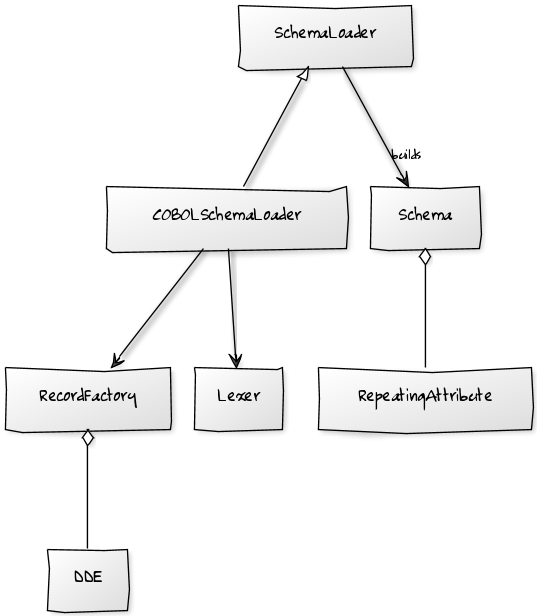
\includegraphics{cobol_loader.png}


\paragraph{Overheads}
\label{cobol_loader:overheads}
Ultimately, we're writing a new {\hyperref[schema_loader:schema.loader.ExternalSchemaLoader]{\code{schema.loader.ExternalSchemaLoader}}}.
The purpose of this is to build a {\hyperref[schema:schema.Schema]{\code{schema.Schema}}} instance
from COBOL source instead of some other source.

\begin{Verbatim}[commandchars=\\\{\}]
\PYG{l+s+sd}{\PYGZdq{}\PYGZdq{}\PYGZdq{}stingray.cobol.loader \PYGZhy{}\PYGZhy{} Parse a COBOL DDE and build a usable Schema.\PYGZdq{}\PYGZdq{}\PYGZdq{}}
\PYG{k+kn}{import} \PYG{n+nn}{re}
\PYG{k+kn}{from} \PYG{n+nn}{collections} \PYG{k+kn}{import} \PYG{n}{namedtuple}\PYG{p}{,} \PYG{n}{Iterator}
\PYG{k+kn}{import} \PYG{n+nn}{logging}
\PYG{k+kn}{import} \PYG{n+nn}{weakref}
\PYG{k+kn}{import} \PYG{n+nn}{warnings}
\PYG{k+kn}{import} \PYG{n+nn}{sys}

\PYG{k+kn}{import} \PYG{n+nn}{stingray.schema.loader}
\PYG{k+kn}{import} \PYG{n+nn}{stingray.cobol}
\PYG{k+kn}{import} \PYG{n+nn}{stingray.cobol.defs}
\end{Verbatim}

We'll put in a version number, just to support some debugging.

\begin{Verbatim}[commandchars=\\\{\}]
\PYG{n}{\PYGZus{}\PYGZus{}version\PYGZus{}\PYGZus{}} \PYG{o}{=} \PYG{l+s}{\PYGZdq{}}\PYG{l+s}{4.4.6}\PYG{l+s}{\PYGZdq{}}
\end{Verbatim}

A module-level logger.

\begin{Verbatim}[commandchars=\\\{\}]
\PYG{n}{logger}\PYG{o}{=} \PYG{n}{logging}\PYG{o}{.}\PYG{n}{getLogger}\PYG{p}{(} \PYG{n}{\PYGZus{}\PYGZus{}name\PYGZus{}\PYGZus{}} \PYG{p}{)}
\end{Verbatim}


\paragraph{Parsing Exceptions}
\label{cobol_loader:parsing-exceptions}\index{SyntaxError (class in cobol.loader)}

\begin{fulllineitems}
\phantomsection\label{cobol_loader:cobol.loader.SyntaxError}\pysigline{\strong{class }\code{cobol.loader.}\bfcode{SyntaxError}}
These are compilation problems.  We have syntax which
is utterly baffling.

\end{fulllineitems}


\begin{Verbatim}[commandchars=\\\{\}]
\PYG{k}{class} \PYG{n+nc}{SyntaxError}\PYG{p}{(} \PYG{n+ne}{Exception} \PYG{p}{)}\PYG{p}{:}
    \PYG{l+s+sd}{\PYGZdq{}\PYGZdq{}\PYGZdq{}COBOL syntax error.\PYGZdq{}\PYGZdq{}\PYGZdq{}}
    \PYG{k}{pass}
\end{Verbatim}


\paragraph{Picture Clause Parsing}
\label{cobol_loader:picture-clause-parsing}
Picture clause parsing is done as the DDE element is created.  Not for a great
reason.  It's derived data from the source picture clause.

It could be done in the parser, also.

Since \code{9(5)V99} is common, precision is easily the characters after the ''.'' or ``V''.
However, there can be several ()'d groups of numbers \code{9(5)V9(3)} kind of of thing.
So precision in the latter case is 3, making things a little more complex.

Also, we don't handle separate sign very gracefully. It seems little-used, so
we're comfortable ignoring it.
\index{Picture (class in cobol.loader)}

\begin{fulllineitems}
\phantomsection\label{cobol_loader:cobol.loader.Picture}\pysigline{\strong{class }\code{cobol.loader.}\bfcode{Picture}}
Define the various attribtes of a COBOL PICTURE clause.
\index{final (cobol.loader.Picture attribute)}

\begin{fulllineitems}
\phantomsection\label{cobol_loader:cobol.loader.Picture.final}\pysigline{\bfcode{final}}
the final picture

\end{fulllineitems}

\index{alpha (cobol.loader.Picture attribute)}

\begin{fulllineitems}
\phantomsection\label{cobol_loader:cobol.loader.Picture.alpha}\pysigline{\bfcode{alpha}}
boolean; True if any \code{"X"} or \code{"A"}; False if all \code{"9"} and related

\end{fulllineitems}

\index{length (cobol.loader.Picture attribute)}

\begin{fulllineitems}
\phantomsection\label{cobol_loader:cobol.loader.Picture.length}\pysigline{\bfcode{length}}
length of the final picture

\end{fulllineitems}

\index{scale (cobol.loader.Picture attribute)}

\begin{fulllineitems}
\phantomsection\label{cobol_loader:cobol.loader.Picture.scale}\pysigline{\bfcode{scale}}
count of \code{"P"} positions, often zero

\end{fulllineitems}

\index{precision (cobol.loader.Picture attribute)}

\begin{fulllineitems}
\phantomsection\label{cobol_loader:cobol.loader.Picture.precision}\pysigline{\bfcode{precision}}
digits to the right of the decimal point

\end{fulllineitems}

\index{signed (cobol.loader.Picture attribute)}

\begin{fulllineitems}
\phantomsection\label{cobol_loader:cobol.loader.Picture.signed}\pysigline{\bfcode{signed}}
boolean; True if any \code{"S"}, \code{"-"} or related

\end{fulllineitems}

\index{decimal (cobol.loader.Picture attribute)}

\begin{fulllineitems}
\phantomsection\label{cobol_loader:cobol.loader.Picture.decimal}\pysigline{\bfcode{decimal}}
\code{"."} or \code{"V"} or \code{None}

\end{fulllineitems}


\end{fulllineitems}


\begin{Verbatim}[commandchars=\\\{\}]
\PYG{n}{Picture} \PYG{o}{=} \PYG{n}{namedtuple}\PYG{p}{(} \PYG{l+s}{\PYGZsq{}}\PYG{l+s}{Picture}\PYG{l+s}{\PYGZsq{}}\PYG{p}{,}
    \PYG{l+s}{\PYGZsq{}}\PYG{l+s}{final, alpha, length, scale, precision, signed, decimal}\PYG{l+s}{\PYGZsq{}} \PYG{p}{)}
\end{Verbatim}
\index{picture\_parser() (in module cobol.loader)}

\begin{fulllineitems}
\phantomsection\label{cobol_loader:cobol.loader.picture_parser}\pysiglinewithargsret{\code{cobol.loader.}\bfcode{picture\_parser}}{\emph{pic}}{}
Parse the text of a PICTURE definition.

\end{fulllineitems}


\begin{Verbatim}[commandchars=\\\{\}]
\PYG{k}{def} \PYG{n+nf}{picture\PYGZus{}parser}\PYG{p}{(} \PYG{n}{pic} \PYG{p}{)}\PYG{p}{:}
    \PYG{l+s+sd}{\PYGZdq{}\PYGZdq{}\PYGZdq{}Rewrite a picture clause to eliminate ()\PYGZsq{}s, S\PYGZsq{}s, V\PYGZsq{}s, P\PYGZsq{}s, etc.}
\PYG{l+s+sd}{    :param pic: Sounce text.}
\PYG{l+s+sd}{    :returns: Picture instance: final, alpha, len(final), scale,}
\PYG{l+s+sd}{        precision, signed, decimal}
\PYG{l+s+sd}{    \PYGZdq{}\PYGZdq{}\PYGZdq{}}
    \PYG{n}{out}\PYG{o}{=} \PYG{p}{[}\PYG{p}{]}
    \PYG{n}{scale}\PYG{p}{,} \PYG{n}{precision}\PYG{p}{,} \PYG{n}{signed}\PYG{p}{,} \PYG{n}{decimal} \PYG{o}{=} \PYG{l+m+mi}{0}\PYG{p}{,} \PYG{l+m+mi}{0}\PYG{p}{,} \PYG{n+nb+bp}{False}\PYG{p}{,} \PYG{n+nb+bp}{None}
    \PYG{n}{char\PYGZus{}iter}\PYG{o}{=} \PYG{n+nb}{iter}\PYG{p}{(}\PYG{n}{pic}\PYG{p}{)}
    \PYG{k}{for} \PYG{n}{c} \PYG{o+ow}{in} \PYG{n}{char\PYGZus{}iter}\PYG{p}{:}
        \PYG{k}{if} \PYG{n}{c} \PYG{o+ow}{in} \PYG{p}{(}\PYG{l+s}{\PYGZsq{}}\PYG{l+s}{A}\PYG{l+s}{\PYGZsq{}}\PYG{p}{,}\PYG{l+s}{\PYGZsq{}}\PYG{l+s}{B}\PYG{l+s}{\PYGZsq{}}\PYG{p}{,}\PYG{l+s}{\PYGZsq{}}\PYG{l+s}{X}\PYG{l+s}{\PYGZsq{}}\PYG{p}{,}\PYG{l+s}{\PYGZsq{}}\PYG{l+s}{Z}\PYG{l+s}{\PYGZsq{}}\PYG{p}{,}\PYG{l+s}{\PYGZsq{}}\PYG{l+s}{9}\PYG{l+s}{\PYGZsq{}}\PYG{p}{,}\PYG{l+s}{\PYGZsq{}}\PYG{l+s}{0}\PYG{l+s}{\PYGZsq{}}\PYG{p}{,}\PYG{l+s}{\PYGZsq{}}\PYG{l+s}{/}\PYG{l+s}{\PYGZsq{}}\PYG{p}{,}\PYG{l+s}{\PYGZsq{}}\PYG{l+s}{,}\PYG{l+s}{\PYGZsq{}}\PYG{p}{,}\PYG{l+s}{\PYGZsq{}}\PYG{l+s}{+}\PYG{l+s}{\PYGZsq{}}\PYG{p}{,}\PYG{l+s}{\PYGZsq{}}\PYG{l+s}{\PYGZhy{}}\PYG{l+s}{\PYGZsq{}}\PYG{p}{,}\PYG{l+s}{\PYGZsq{}}\PYG{l+s}{*}\PYG{l+s}{\PYGZsq{}}\PYG{p}{,}\PYG{l+s}{\PYGZsq{}}\PYG{l+s}{\PYGZdl{}}\PYG{l+s}{\PYGZsq{}}\PYG{p}{)}\PYG{p}{:}
            \PYG{n}{out}\PYG{o}{.}\PYG{n}{append}\PYG{p}{(} \PYG{n}{c} \PYG{p}{)}
            \PYG{k}{if} \PYG{n}{decimal}\PYG{p}{:} \PYG{n}{precision} \PYG{o}{+}\PYG{o}{=} \PYG{l+m+mi}{1}
        \PYG{k}{elif} \PYG{n}{c} \PYG{o}{==} \PYG{l+s}{\PYGZsq{}}\PYG{l+s}{D}\PYG{l+s}{\PYGZsq{}}\PYG{p}{:}
            \PYG{n}{nc}\PYG{o}{=} \PYG{n+nb}{next}\PYG{p}{(}\PYG{n}{char\PYGZus{}iter}\PYG{p}{)}
            \PYG{k}{assert} \PYG{n}{nc} \PYG{o}{==} \PYG{l+s}{\PYGZdq{}}\PYG{l+s}{B}\PYG{l+s}{\PYGZdq{}}\PYG{p}{,} \PYG{l+s}{\PYGZdq{}}\PYG{l+s}{picture error in \PYGZob{}0!r\PYGZcb{}}\PYG{l+s}{\PYGZdq{}}\PYG{o}{.}\PYG{n}{format}\PYG{p}{(}\PYG{n}{pic}\PYG{p}{)}
            \PYG{n}{out}\PYG{o}{.}\PYG{n}{append}\PYG{p}{(} \PYG{l+s}{\PYGZdq{}}\PYG{l+s}{DB}\PYG{l+s}{\PYGZdq{}} \PYG{p}{)}
            \PYG{n}{signed}\PYG{o}{=} \PYG{n+nb+bp}{True}
        \PYG{k}{elif} \PYG{n}{c} \PYG{o}{==}  \PYG{l+s}{\PYGZsq{}}\PYG{l+s}{C}\PYG{l+s}{\PYGZsq{}}\PYG{p}{:}
            \PYG{n}{nc}\PYG{o}{=} \PYG{n+nb}{next}\PYG{p}{(}\PYG{n}{char\PYGZus{}iter}\PYG{p}{)}
            \PYG{k}{assert} \PYG{n}{nc} \PYG{o}{==} \PYG{l+s}{\PYGZdq{}}\PYG{l+s}{R}\PYG{l+s}{\PYGZdq{}}\PYG{p}{,} \PYG{l+s}{\PYGZdq{}}\PYG{l+s}{picture error in \PYGZob{}0!r\PYGZcb{}}\PYG{l+s}{\PYGZdq{}}\PYG{o}{.}\PYG{n}{format}\PYG{p}{(}\PYG{n}{pic}\PYG{p}{)}
            \PYG{n}{out}\PYG{o}{.}\PYG{n}{append}\PYG{p}{(} \PYG{l+s}{\PYGZdq{}}\PYG{l+s}{CR}\PYG{l+s}{\PYGZdq{}} \PYG{p}{)}
            \PYG{n}{signed}\PYG{o}{=} \PYG{n+nb+bp}{True}
        \PYG{k}{elif} \PYG{n}{c} \PYG{o}{==} \PYG{l+s}{\PYGZsq{}}\PYG{l+s}{(}\PYG{l+s}{\PYGZsq{}}\PYG{p}{:}
            \PYG{n}{irpt}\PYG{o}{=} \PYG{l+m+mi}{0}
            \PYG{k}{try}\PYG{p}{:}
                \PYG{k}{for} \PYG{n}{c} \PYG{o+ow}{in} \PYG{n}{char\PYGZus{}iter}\PYG{p}{:}
                    \PYG{k}{if} \PYG{n}{c} \PYG{o}{==} \PYG{l+s}{\PYGZsq{}}\PYG{l+s}{)}\PYG{l+s}{\PYGZsq{}}\PYG{p}{:} \PYG{k}{break}
                    \PYG{n}{irpt} \PYG{o}{=} \PYG{l+m+mi}{10}\PYG{o}{*}\PYG{n}{irpt} \PYG{o}{+} \PYG{n+nb}{int}\PYG{p}{(} \PYG{n}{c} \PYG{p}{)}
            \PYG{k}{except} \PYG{n+ne}{ValueError} \PYG{k}{as} \PYG{n}{e}\PYG{p}{:}
                \PYG{k}{raise} \PYG{n+ne}{SyntaxError}\PYG{p}{(} \PYG{l+s}{\PYGZdq{}}\PYG{l+s}{picture error in \PYGZob{}0!r\PYGZcb{}}\PYG{l+s}{\PYGZdq{}}\PYG{o}{.}\PYG{n}{format}\PYG{p}{(}\PYG{n}{pic}\PYG{p}{)} \PYG{p}{)}
            \PYG{k}{assert} \PYG{n}{c} \PYG{o}{==} \PYG{l+s}{\PYGZsq{}}\PYG{l+s}{)}\PYG{l+s}{\PYGZsq{}}\PYG{p}{,}  \PYG{l+s}{\PYGZdq{}}\PYG{l+s}{picture error in \PYGZob{}0!r\PYGZcb{}}\PYG{l+s}{\PYGZdq{}}\PYG{o}{.}\PYG{n}{format}\PYG{p}{(}\PYG{n}{pic}\PYG{p}{)}
            \PYG{n}{out}\PYG{o}{.}\PYG{n}{append}\PYG{p}{(} \PYG{p}{(}\PYG{n}{irpt}\PYG{o}{\PYGZhy{}}\PYG{l+m+mi}{1}\PYG{p}{)}\PYG{o}{*}\PYG{n}{out}\PYG{p}{[}\PYG{o}{\PYGZhy{}}\PYG{l+m+mi}{1}\PYG{p}{]} \PYG{p}{)}
            \PYG{k}{if} \PYG{n}{decimal}\PYG{p}{:} \PYG{n}{precision} \PYG{o}{+}\PYG{o}{=} \PYG{n}{irpt}\PYG{o}{\PYGZhy{}}\PYG{l+m+mi}{1}
        \PYG{k}{elif} \PYG{n}{c} \PYG{o}{==} \PYG{l+s}{\PYGZsq{}}\PYG{l+s}{S}\PYG{l+s}{\PYGZsq{}}\PYG{p}{:}
            \PYG{c}{\PYGZsh{} silently drop an \PYGZdq{}S\PYGZdq{}.}
            \PYG{c}{\PYGZsh{} Note that \PYGZsq{}S\PYGZsq{} plus a SIGN SEPARATE option increases the size of the picture!}
            \PYG{n}{signed}\PYG{o}{=} \PYG{n+nb+bp}{True}
        \PYG{k}{elif} \PYG{n}{c}  \PYG{o}{==} \PYG{l+s}{\PYGZsq{}}\PYG{l+s}{P}\PYG{l+s}{\PYGZsq{}}\PYG{p}{:}
            \PYG{c}{\PYGZsh{} \PYGZdq{}P\PYGZdq{} sets scale and isn\PYGZsq{}t represented.}
            \PYG{n}{scale} \PYG{o}{+}\PYG{o}{=} \PYG{l+m+mi}{1}
        \PYG{k}{elif} \PYG{n}{c}  \PYG{o}{==} \PYG{l+s}{\PYGZdq{}}\PYG{l+s}{V}\PYG{l+s}{\PYGZdq{}}\PYG{p}{:}
            \PYG{c}{\PYGZsh{} \PYGZdq{}V\PYGZdq{} sets precision and isn\PYGZsq{}t represented.}
            \PYG{n}{decimal}\PYG{o}{=} \PYG{l+s}{\PYGZdq{}}\PYG{l+s}{V}\PYG{l+s}{\PYGZdq{}}
        \PYG{k}{elif} \PYG{n}{c}  \PYG{o}{==} \PYG{l+s}{\PYGZdq{}}\PYG{l+s}{.}\PYG{l+s}{\PYGZdq{}}\PYG{p}{:}
            \PYG{n}{decimal}\PYG{o}{=} \PYG{l+s}{\PYGZdq{}}\PYG{l+s}{.}\PYG{l+s}{\PYGZdq{}}
            \PYG{n}{out}\PYG{o}{.}\PYG{n}{append}\PYG{p}{(} \PYG{l+s}{\PYGZdq{}}\PYG{l+s}{.}\PYG{l+s}{\PYGZdq{}} \PYG{p}{)}
        \PYG{k}{else}\PYG{p}{:}
            \PYG{k}{raise} \PYG{n+ne}{SyntaxError}\PYG{p}{(} \PYG{l+s}{\PYGZdq{}}\PYG{l+s}{Picture error in \PYGZob{}!r\PYGZcb{}}\PYG{l+s}{\PYGZdq{}}\PYG{o}{.}\PYG{n}{format}\PYG{p}{(}\PYG{n}{pic}\PYG{p}{)} \PYG{p}{)}

    \PYG{n}{final}\PYG{o}{=} \PYG{l+s}{\PYGZdq{}}\PYG{l+s}{\PYGZdq{}}\PYG{o}{.}\PYG{n}{join}\PYG{p}{(} \PYG{n}{out} \PYG{p}{)}
    \PYG{n}{alpha}\PYG{o}{=} \PYG{p}{(}\PYG{l+s}{\PYGZsq{}}\PYG{l+s}{A}\PYG{l+s}{\PYGZsq{}} \PYG{o+ow}{in} \PYG{n}{final}\PYG{p}{)} \PYG{o+ow}{or} \PYG{p}{(}\PYG{l+s}{\PYGZsq{}}\PYG{l+s}{X}\PYG{l+s}{\PYGZsq{}} \PYG{o+ow}{in} \PYG{n}{final}\PYG{p}{)} \PYG{o+ow}{or} \PYG{p}{(}\PYG{l+s}{\PYGZsq{}}\PYG{l+s}{/}\PYG{l+s}{\PYGZsq{}} \PYG{o+ow}{in} \PYG{n}{final}\PYG{p}{)}
    \PYG{n}{logger}\PYG{o}{.}\PYG{n}{debug}\PYG{p}{(} \PYG{l+s}{\PYGZdq{}}\PYG{l+s}{PIC \PYGZob{}0\PYGZcb{} \PYGZob{}1\PYGZcb{} alpha=\PYGZob{}2\PYGZcb{} scale=\PYGZob{}3\PYGZcb{} prec=\PYGZob{}4\PYGZcb{}}\PYG{l+s}{\PYGZdq{}}\PYG{o}{.}\PYG{n}{format}\PYG{p}{(}\PYG{n}{pic}\PYG{p}{,} \PYG{n}{final}\PYG{p}{,} \PYG{n}{alpha}\PYG{p}{,} \PYG{n}{scale}\PYG{p}{,} \PYG{n}{precision}\PYG{p}{)} \PYG{p}{)}
    \PYG{c}{\PYGZsh{} Note: Actual bytes consumed depends on len(final) and usage!}
    \PYG{k}{return} \PYG{n}{Picture}\PYG{p}{(} \PYG{n}{final}\PYG{p}{,} \PYG{n}{alpha}\PYG{p}{,} \PYG{n+nb}{len}\PYG{p}{(}\PYG{n}{final}\PYG{p}{)}\PYG{p}{,} \PYG{n}{scale}\PYG{p}{,}
        \PYG{n}{precision}\PYG{p}{,} \PYG{n}{signed}\PYG{p}{,} \PYG{n}{decimal}\PYG{p}{)}
\end{Verbatim}


\paragraph{Lexical Scanning}
\label{cobol_loader:lexical-scanning}
The lexical scanner can be subclassed to extend its capability.  The default
lexical scanner provides a {\hyperref[cobol_loader:cobol.loader.Lexer.clean]{\code{Lexer.clean()}}} method that simply removes comments.
This may need to be overridden to remove line numbers (from positions 72-80),
module identification (from positions 1-5), and format control directives.

Also, we have to deal with ``Compiler Directing Statements'': EJECT, SKIP1, SKIP2 and SKIP3.
These are simply noise that may appear in the source.
\index{Lexer (class in cobol.loader)}

\begin{fulllineitems}
\phantomsection\label{cobol_loader:cobol.loader.Lexer}\pysigline{\strong{class }\code{cobol.loader.}\bfcode{Lexer}}
Basic lexer that simply removes comments and the first six positions of each line.

\end{fulllineitems}


\begin{Verbatim}[commandchars=\\\{\}]
\PYG{k}{class} \PYG{n+nc}{Lexer}\PYG{p}{:}
    \PYG{l+s+sd}{\PYGZdq{}\PYGZdq{}\PYGZdq{}Lexical scanner for COBOL.  Iterates over tokens in source text.\PYGZdq{}\PYGZdq{}\PYGZdq{}}
    \PYG{n}{separator}\PYG{o}{=} \PYG{n}{re}\PYG{o}{.}\PYG{n}{compile}\PYG{p}{(} \PYG{l+s}{r\PYGZsq{}}\PYG{l+s}{[.,;]?}\PYG{l+s}{\PYGZbs{}}\PYG{l+s}{s}\PYG{l+s}{\PYGZsq{}} \PYG{p}{)}
    \PYG{n}{quote1}\PYG{o}{=} \PYG{n}{re}\PYG{o}{.}\PYG{n}{compile}\PYG{p}{(} \PYG{l+s}{r\PYGZdq{}}\PYG{l+s}{\PYGZsq{}}\PYG{l+s}{[\PYGZca{}}\PYG{l+s}{\PYGZsq{}}\PYG{l+s}{]*}\PYG{l+s}{\PYGZsq{}}\PYG{l+s}{\PYGZdq{}} \PYG{p}{)}
    \PYG{n}{quote2}\PYG{o}{=} \PYG{n}{re}\PYG{o}{.}\PYG{n}{compile}\PYG{p}{(} \PYG{l+s}{r\PYGZsq{}}\PYG{l+s}{\PYGZdq{}}\PYG{l+s}{[\PYGZca{}}\PYG{l+s}{\PYGZdq{}}\PYG{l+s}{]*}\PYG{l+s}{\PYGZdq{}}\PYG{l+s}{\PYGZsq{}} \PYG{p}{)}
    \PYG{k}{def} \PYG{n+nf}{\PYGZus{}\PYGZus{}init\PYGZus{}\PYGZus{}}\PYG{p}{(} \PYG{n+nb+bp}{self}\PYG{p}{,} \PYG{n}{replacing}\PYG{o}{=}\PYG{n+nb+bp}{None} \PYG{p}{)}\PYG{p}{:}
        \PYG{n+nb+bp}{self}\PYG{o}{.}\PYG{n}{log}\PYG{o}{=} \PYG{n}{logging}\PYG{o}{.}\PYG{n}{getLogger}\PYG{p}{(} \PYG{n+nb+bp}{self}\PYG{o}{.}\PYG{n}{\PYGZus{}\PYGZus{}class\PYGZus{}\PYGZus{}}\PYG{o}{.}\PYG{n}{\PYGZus{}\PYGZus{}qualname\PYGZus{}\PYGZus{}} \PYG{p}{)}
        \PYG{n+nb+bp}{self}\PYG{o}{.}\PYG{n}{replacing}\PYG{o}{=} \PYG{n}{replacing} \PYG{o+ow}{or} \PYG{p}{[}\PYG{p}{]}
\end{Verbatim}
\index{clean() (cobol.loader.Lexer method)}

\begin{fulllineitems}
\phantomsection\label{cobol_loader:cobol.loader.Lexer.clean}\pysiglinewithargsret{\code{Lexer.}\bfcode{clean}}{\emph{line}}{}
The default process for cleaning a line. Simply rstrip trailing spaces.

\end{fulllineitems}


\begin{Verbatim}[commandchars=\\\{\}]
\PYG{k}{def} \PYG{n+nf}{clean}\PYG{p}{(} \PYG{n+nb+bp}{self}\PYG{p}{,} \PYG{n}{line} \PYG{p}{)}\PYG{p}{:}
    \PYG{l+s+sd}{\PYGZdq{}\PYGZdq{}\PYGZdq{}Default cleaner removes positions 0:6.\PYGZdq{}\PYGZdq{}\PYGZdq{}}
    \PYG{k}{return} \PYG{n}{line}\PYG{p}{[}\PYG{l+m+mi}{6}\PYG{p}{:}\PYG{p}{]}\PYG{o}{.}\PYG{n}{rstrip}\PYG{p}{(}\PYG{p}{)}
\end{Verbatim}
\index{scan() (cobol.loader.Lexer method)}

\begin{fulllineitems}
\phantomsection\label{cobol_loader:cobol.loader.Lexer.scan}\pysiglinewithargsret{\code{Lexer.}\bfcode{scan}}{\emph{text}}{}
Locate the sequence of tokens in the input stream.

\end{fulllineitems}


\begin{Verbatim}[commandchars=\\\{\}]
\PYG{k}{def} \PYG{n+nf}{scan}\PYG{p}{(} \PYG{n+nb+bp}{self}\PYG{p}{,} \PYG{n}{text} \PYG{p}{)}\PYG{p}{:}
    \PYG{l+s+sd}{\PYGZdq{}\PYGZdq{}\PYGZdq{}Locate the next token in the input stream.}
\PYG{l+s+sd}{    \PYGZhy{} Clean 6\PYGZhy{}char lead\PYGZhy{}in plus trailing whitespace}
\PYG{l+s+sd}{    \PYGZhy{} Add one extra space to distinguish end\PYGZhy{}of\PYGZhy{}line {}`{}`\PYGZsq{}. \PYGZsq{}{}`{}`}
\PYG{l+s+sd}{      from picture clause.}
\PYG{l+s+sd}{    \PYGZdq{}\PYGZdq{}\PYGZdq{}}
    \PYG{k}{if} \PYG{n+nb}{isinstance}\PYG{p}{(}\PYG{n}{text}\PYG{p}{,} \PYG{p}{(}\PYG{n+nb}{str}\PYG{p}{,} \PYG{n+nb}{bytes}\PYG{p}{)}\PYG{p}{)}\PYG{p}{:}
        \PYG{n}{text}\PYG{o}{=} \PYG{n}{text}\PYG{o}{.}\PYG{n}{splitlines}\PYG{p}{(}\PYG{p}{)}
    \PYG{n+nb+bp}{self}\PYG{o}{.}\PYG{n}{all\PYGZus{}lines}\PYG{o}{=} \PYG{p}{(} \PYG{n+nb+bp}{self}\PYG{o}{.}\PYG{n}{clean}\PYG{p}{(}\PYG{n}{line}\PYG{p}{)} \PYG{o}{+} \PYG{l+s}{\PYGZsq{}}\PYG{l+s}{ }\PYG{l+s}{\PYGZsq{}}
        \PYG{k}{for} \PYG{n}{line} \PYG{o+ow}{in} \PYG{n}{text} \PYG{p}{)}
    \PYG{c}{\PYGZsh{} Remove comments, blank lines and compiler directives}
    \PYG{n+nb+bp}{self}\PYG{o}{.}\PYG{n}{lines} \PYG{o}{=} \PYG{p}{(} \PYG{n}{line}
        \PYG{k}{for} \PYG{n}{line} \PYG{o+ow}{in} \PYG{n+nb+bp}{self}\PYG{o}{.}\PYG{n}{all\PYGZus{}lines}
            \PYG{k}{if} \PYG{n}{line} \PYG{o+ow}{and} \PYG{n}{line}\PYG{p}{[}\PYG{l+m+mi}{0}\PYG{p}{]} \PYG{o+ow}{not} \PYG{o+ow}{in} \PYG{p}{(}\PYG{l+s}{\PYGZsq{}}\PYG{l+s}{*}\PYG{l+s}{\PYGZsq{}}\PYG{p}{,} \PYG{l+s}{\PYGZsq{}}\PYG{l+s}{/}\PYG{l+s}{\PYGZsq{}}\PYG{p}{)}
            \PYG{o+ow}{and} \PYG{n}{line}\PYG{o}{.}\PYG{n}{strip}\PYG{p}{(}\PYG{p}{)} \PYG{o+ow}{not} \PYG{o+ow}{in} \PYG{p}{(}\PYG{l+s}{\PYGZdq{}}\PYG{l+s}{EJECT}\PYG{l+s}{\PYGZdq{}}\PYG{p}{,} \PYG{l+s}{\PYGZdq{}}\PYG{l+s}{SKIP1}\PYG{l+s}{\PYGZdq{}}\PYG{p}{,} \PYG{l+s}{\PYGZdq{}}\PYG{l+s}{SKIP2}\PYG{l+s}{\PYGZdq{}}\PYG{p}{,} \PYG{l+s}{\PYGZdq{}}\PYG{l+s}{SKIP3}\PYG{l+s}{\PYGZdq{}}\PYG{p}{)} \PYG{p}{)}
    \PYG{c}{\PYGZsh{} Break remaining lines into words}
    \PYG{k}{for} \PYG{n}{line} \PYG{o+ow}{in} \PYG{n+nb+bp}{self}\PYG{o}{.}\PYG{n}{lines}\PYG{p}{:}
        \PYG{k}{if} \PYG{n+nb}{len}\PYG{p}{(}\PYG{n}{line}\PYG{p}{)} \PYG{o}{==} \PYG{l+m+mi}{0}\PYG{p}{:} \PYG{k}{continue}
        \PYG{n}{logger}\PYG{o}{.}\PYG{n}{debug}\PYG{p}{(} \PYG{n}{line} \PYG{p}{)}
        \PYG{c}{\PYGZsh{} Apply all replacing rules.}
        \PYG{k}{for} \PYG{n}{old}\PYG{p}{,} \PYG{n}{new} \PYG{o+ow}{in} \PYG{n+nb+bp}{self}\PYG{o}{.}\PYG{n}{replacing}\PYG{p}{:}
            \PYG{n}{line}\PYG{o}{=} \PYG{n}{line}\PYG{o}{.}\PYG{n}{replace}\PYG{p}{(}\PYG{n}{old}\PYG{p}{,}\PYG{n}{new}\PYG{p}{)}
        \PYG{k}{if} \PYG{n+nb+bp}{self}\PYG{o}{.}\PYG{n}{replacing}\PYG{p}{:} \PYG{n}{logger}\PYG{o}{.}\PYG{n}{debug}\PYG{p}{(} \PYG{l+s}{\PYGZdq{}}\PYG{l+s}{Post\PYGZhy{}Replacing \PYGZob{}!r\PYGZcb{}}\PYG{l+s}{\PYGZdq{}}\PYG{o}{.}\PYG{n}{format}\PYG{p}{(}\PYG{n}{line}\PYG{p}{)} \PYG{p}{)}
        \PYG{n}{current}\PYG{o}{=} \PYG{n}{line}\PYG{o}{.}\PYG{n}{lstrip}\PYG{p}{(}\PYG{p}{)}
        \PYG{k}{while} \PYG{n}{current}\PYG{p}{:}
            \PYG{k}{if} \PYG{n}{current}\PYG{p}{[}\PYG{l+m+mi}{0}\PYG{p}{]} \PYG{o}{==} \PYG{l+s}{\PYGZdq{}}\PYG{l+s}{\PYGZsq{}}\PYG{l+s}{\PYGZdq{}}\PYG{p}{:}
                \PYG{c}{\PYGZsh{} apostrophe string, break on balancing apostrophe}
                \PYG{n}{match}\PYG{o}{=} \PYG{n+nb+bp}{self}\PYG{o}{.}\PYG{n}{quote1}\PYG{o}{.}\PYG{n}{match}\PYG{p}{(} \PYG{n}{current} \PYG{p}{)}
                \PYG{n}{space}\PYG{o}{=} \PYG{n}{match}\PYG{o}{.}\PYG{n}{end}\PYG{p}{(}\PYG{p}{)}
            \PYG{k}{elif} \PYG{n}{current}\PYG{p}{[}\PYG{l+m+mi}{0}\PYG{p}{]} \PYG{o}{==} \PYG{l+s}{\PYGZsq{}}\PYG{l+s}{\PYGZdq{}}\PYG{l+s}{\PYGZsq{}}\PYG{p}{:}
                \PYG{c}{\PYGZsh{} quote string, break on balancing quote}
                \PYG{n}{match}\PYG{o}{=} \PYG{n+nb+bp}{self}\PYG{o}{.}\PYG{n}{quote2}\PYG{o}{.}\PYG{n}{match}\PYG{p}{(} \PYG{n}{current} \PYG{p}{)}
                \PYG{n}{space}\PYG{o}{=} \PYG{n}{match}\PYG{o}{.}\PYG{n}{end}\PYG{p}{(}\PYG{p}{)}
            \PYG{k}{else}\PYG{p}{:}
                \PYG{n}{match}\PYG{o}{=} \PYG{n+nb+bp}{self}\PYG{o}{.}\PYG{n}{separator}\PYG{o}{.}\PYG{n}{search}\PYG{p}{(} \PYG{n}{current} \PYG{p}{)}
                \PYG{n}{space}\PYG{o}{=} \PYG{n}{match}\PYG{o}{.}\PYG{n}{start}\PYG{p}{(}\PYG{p}{)}
                \PYG{k}{if} \PYG{n}{space} \PYG{o}{==} \PYG{l+m+mi}{0}\PYG{p}{:} \PYG{c}{\PYGZsh{} starts with separator}
                    \PYG{n}{space}\PYG{o}{=} \PYG{n}{match}\PYG{o}{.}\PYG{n}{end}\PYG{p}{(}\PYG{p}{)}\PYG{o}{\PYGZhy{}}\PYG{l+m+mi}{1}
            \PYG{n}{token}\PYG{p}{,} \PYG{n}{current} \PYG{o}{=} \PYG{n}{current}\PYG{p}{[}\PYG{p}{:}\PYG{n}{space}\PYG{p}{]}\PYG{p}{,} \PYG{n}{current}\PYG{p}{[}\PYG{n}{space}\PYG{p}{:}\PYG{p}{]}\PYG{o}{.}\PYG{n}{lstrip}\PYG{p}{(}\PYG{p}{)}
            \PYG{n+nb+bp}{self}\PYG{o}{.}\PYG{n}{log}\PYG{o}{.}\PYG{n}{debug}\PYG{p}{(} \PYG{n}{token} \PYG{p}{)}
            \PYG{k}{yield} \PYG{n}{token}
\end{Verbatim}
\index{Lexer\_Long\_Lines (class in cobol.loader)}

\begin{fulllineitems}
\phantomsection\label{cobol_loader:cobol.loader.Lexer_Long_Lines}\pysigline{\strong{class }\code{cobol.loader.}\bfcode{Lexer\_Long\_Lines}}
More sophisticated lexer that removes the first six positions of each line.
If the line is over 72 positions, it also removes positions {[}71:80{]}.
Since it's an extension to {\hyperref[cobol_loader:cobol.loader.Lexer]{\code{cobol.loader.Lexer}}}, it also removes comments.

\end{fulllineitems}


\begin{Verbatim}[commandchars=\\\{\}]
\PYG{k}{class} \PYG{n+nc}{Lexer\PYGZus{}Long\PYGZus{}Lines}\PYG{p}{(} \PYG{n}{Lexer} \PYG{p}{)}\PYG{p}{:}

    \PYG{k}{def} \PYG{n+nf}{clean}\PYG{p}{(} \PYG{n+nb+bp}{self}\PYG{p}{,} \PYG{n}{line} \PYG{p}{)}\PYG{p}{:}
        \PYG{l+s+sd}{\PYGZdq{}\PYGZdq{}\PYGZdq{}Remove positions 72:80 and 0:6.\PYGZdq{}\PYGZdq{}\PYGZdq{}}
        \PYG{k}{if} \PYG{n+nb}{len}\PYG{p}{(}\PYG{n}{line}\PYG{p}{)} \PYG{o}{\PYGZgt{}} \PYG{l+m+mi}{72}\PYG{p}{:}
            \PYG{k}{return} \PYG{n}{line}\PYG{p}{[}\PYG{l+m+mi}{6}\PYG{p}{:}\PYG{l+m+mi}{72}\PYG{p}{]}\PYG{o}{.}\PYG{n}{strip}\PYG{p}{(}\PYG{p}{)}
        \PYG{k}{return} \PYG{n}{line}\PYG{p}{[}\PYG{l+m+mi}{6}\PYG{p}{:}\PYG{p}{]}\PYG{o}{.}\PYG{n}{rstrip}\PYG{p}{(}\PYG{p}{)}
\end{Verbatim}

We use this by subclassing \code{cobol.COBOLSchemaLoader}.

\begin{Verbatim}[commandchars=\\\{\}]
\PYG{k}{class} \PYG{n+nc}{MySchemaLoader}\PYG{p}{(} \PYG{n}{cobol}\PYG{o}{.}\PYG{n}{COBOLSchemaLoader} \PYG{p}{)}\PYG{p}{:}
    \PYG{n}{lexer\PYGZus{}class}\PYG{o}{=} \PYG{n}{cobol}\PYG{o}{.}\PYG{n}{Lexer\PYGZus{}Long\PYGZus{}Lines}
\end{Verbatim}


\paragraph{Parsing}
\label{cobol_loader:parsing}
The {\hyperref[cobol_loader:cobol.loader.RecordFactory]{\code{cobol.loader.RecordFactory}}} class is the parser for record definitions.
The parser has three basic sets of methods:
\begin{enumerate}
\item {} 
clause parsing methods,

\item {} 
element parsing methods and

\item {} 
complete record layout parsing.

\end{enumerate}
\index{RecordFactory (class in cobol.loader)}

\begin{fulllineitems}
\phantomsection\label{cobol_loader:cobol.loader.RecordFactory}\pysigline{\strong{class }\code{cobol.loader.}\bfcode{RecordFactory}}
Parse a record layout. This means parsing a sequence of DDE's and
assembling them into a proper structure.  Each element consists of a sequence of
individual clauses.

\end{fulllineitems}


\begin{Verbatim}[commandchars=\\\{\}]
\PYG{k}{class} \PYG{n+nc}{RecordFactory}\PYG{p}{:}
    \PYG{l+s+sd}{\PYGZdq{}\PYGZdq{}\PYGZdq{}Parse a copybook, creating a DDE structure.\PYGZdq{}\PYGZdq{}\PYGZdq{}}
    \PYG{n}{noisewords}\PYG{o}{=} \PYG{p}{\PYGZob{}}\PYG{l+s}{\PYGZdq{}}\PYG{l+s}{WHEN}\PYG{l+s}{\PYGZdq{}}\PYG{p}{,}\PYG{l+s}{\PYGZdq{}}\PYG{l+s}{IS}\PYG{l+s}{\PYGZdq{}}\PYG{p}{,}\PYG{l+s}{\PYGZdq{}}\PYG{l+s}{TIMES}\PYG{l+s}{\PYGZdq{}}\PYG{p}{\PYGZcb{}}
    \PYG{n}{keywords}\PYG{o}{=} \PYG{p}{\PYGZob{}}\PYG{l+s}{\PYGZdq{}}\PYG{l+s}{BLANK}\PYG{l+s}{\PYGZdq{}}\PYG{p}{,}\PYG{l+s}{\PYGZdq{}}\PYG{l+s}{ZERO}\PYG{l+s}{\PYGZdq{}}\PYG{p}{,}\PYG{l+s}{\PYGZdq{}}\PYG{l+s}{ZEROS}\PYG{l+s}{\PYGZdq{}}\PYG{p}{,}\PYG{l+s}{\PYGZdq{}}\PYG{l+s}{ZEROES}\PYG{l+s}{\PYGZdq{}}\PYG{p}{,}\PYG{l+s}{\PYGZdq{}}\PYG{l+s}{SPACES}\PYG{l+s}{\PYGZdq{}}\PYG{p}{,}
        \PYG{l+s}{\PYGZdq{}}\PYG{l+s}{DATE}\PYG{l+s}{\PYGZdq{}}\PYG{p}{,}\PYG{l+s}{\PYGZdq{}}\PYG{l+s}{FORMAT}\PYG{l+s}{\PYGZdq{}}\PYG{p}{,}\PYG{l+s}{\PYGZdq{}}\PYG{l+s}{EXTERNAL}\PYG{l+s}{\PYGZdq{}}\PYG{p}{,}\PYG{l+s}{\PYGZdq{}}\PYG{l+s}{GLOBAL}\PYG{l+s}{\PYGZdq{}}\PYG{p}{,}
        \PYG{l+s}{\PYGZdq{}}\PYG{l+s}{JUST}\PYG{l+s}{\PYGZdq{}}\PYG{p}{,}\PYG{l+s}{\PYGZdq{}}\PYG{l+s}{JUSTIFIED}\PYG{l+s}{\PYGZdq{}}\PYG{p}{,}\PYG{l+s}{\PYGZdq{}}\PYG{l+s}{LEFT}\PYG{l+s}{\PYGZdq{}}\PYG{p}{,}\PYG{l+s}{\PYGZdq{}}\PYG{l+s}{RIGHT}\PYG{l+s}{\PYGZdq{}}
        \PYG{l+s}{\PYGZdq{}}\PYG{l+s}{OCCURS}\PYG{l+s}{\PYGZdq{}}\PYG{p}{,}\PYG{l+s}{\PYGZdq{}}\PYG{l+s}{DEPENDING}\PYG{l+s}{\PYGZdq{}}\PYG{p}{,}\PYG{l+s}{\PYGZdq{}}\PYG{l+s}{ON}\PYG{l+s}{\PYGZdq{}}\PYG{p}{,}\PYG{l+s}{\PYGZdq{}}\PYG{l+s}{TIMES}\PYG{l+s}{\PYGZdq{}}\PYG{p}{,}
        \PYG{l+s}{\PYGZdq{}}\PYG{l+s}{PIC}\PYG{l+s}{\PYGZdq{}}\PYG{p}{,}\PYG{l+s}{\PYGZdq{}}\PYG{l+s}{PICTURE}\PYG{l+s}{\PYGZdq{}}\PYG{p}{,}
        \PYG{l+s}{\PYGZdq{}}\PYG{l+s}{REDEFINES}\PYG{l+s}{\PYGZdq{}}\PYG{p}{,}\PYG{l+s}{\PYGZdq{}}\PYG{l+s}{RENAMES}\PYG{l+s}{\PYGZdq{}}\PYG{p}{,}
        \PYG{l+s}{\PYGZdq{}}\PYG{l+s}{SIGN}\PYG{l+s}{\PYGZdq{}}\PYG{p}{,}\PYG{l+s}{\PYGZdq{}}\PYG{l+s}{LEADING}\PYG{l+s}{\PYGZdq{}}\PYG{p}{,}\PYG{l+s}{\PYGZdq{}}\PYG{l+s}{TRAILING}\PYG{l+s}{\PYGZdq{}}\PYG{p}{,}\PYG{l+s}{\PYGZdq{}}\PYG{l+s}{SEPARATE}\PYG{l+s}{\PYGZdq{}}\PYG{p}{,}\PYG{l+s}{\PYGZdq{}}\PYG{l+s}{CHARACTER}\PYG{l+s}{\PYGZdq{}}\PYG{p}{,}
        \PYG{l+s}{\PYGZdq{}}\PYG{l+s}{SYNCH}\PYG{l+s}{\PYGZdq{}}\PYG{p}{,}\PYG{l+s}{\PYGZdq{}}\PYG{l+s}{SYNCHRONIZED}\PYG{l+s}{\PYGZdq{}}\PYG{p}{,}
        \PYG{l+s}{\PYGZdq{}}\PYG{l+s}{USAGE}\PYG{l+s}{\PYGZdq{}}\PYG{p}{,}\PYG{l+s}{\PYGZdq{}}\PYG{l+s}{DISPLAY}\PYG{l+s}{\PYGZdq{}}\PYG{p}{,}\PYG{l+s}{\PYGZdq{}}\PYG{l+s}{COMP\PYGZhy{}3}\PYG{l+s}{\PYGZdq{}}\PYG{p}{,}
        \PYG{l+s}{\PYGZdq{}}\PYG{l+s}{VALUE}\PYG{l+s}{\PYGZdq{}}\PYG{p}{,}\PYG{l+s}{\PYGZdq{}}\PYG{l+s}{.}\PYG{l+s}{\PYGZdq{}}\PYG{p}{\PYGZcb{}}

    \PYG{n}{redefines\PYGZus{}class}\PYG{o}{=} \PYG{n}{stingray}\PYG{o}{.}\PYG{n}{cobol}\PYG{o}{.}\PYG{n}{defs}\PYG{o}{.}\PYG{n}{Redefines}
    \PYG{n}{successor\PYGZus{}class}\PYG{o}{=} \PYG{n}{stingray}\PYG{o}{.}\PYG{n}{cobol}\PYG{o}{.}\PYG{n}{defs}\PYG{o}{.}\PYG{n}{Successor}
    \PYG{n}{group\PYGZus{}class}\PYG{o}{=} \PYG{n}{stingray}\PYG{o}{.}\PYG{n}{cobol}\PYG{o}{.}\PYG{n}{defs}\PYG{o}{.}\PYG{n}{Group}
    \PYG{n}{display\PYGZus{}class}\PYG{o}{=} \PYG{n}{stingray}\PYG{o}{.}\PYG{n}{cobol}\PYG{o}{.}\PYG{n}{defs}\PYG{o}{.}\PYG{n}{UsageDisplay}
    \PYG{n}{comp\PYGZus{}class}\PYG{o}{=} \PYG{n}{stingray}\PYG{o}{.}\PYG{n}{cobol}\PYG{o}{.}\PYG{n}{defs}\PYG{o}{.}\PYG{n}{UsageComp}
    \PYG{n}{comp3\PYGZus{}class}\PYG{o}{=} \PYG{n}{stingray}\PYG{o}{.}\PYG{n}{cobol}\PYG{o}{.}\PYG{n}{defs}\PYG{o}{.}\PYG{n}{UsageComp3}
    \PYG{n}{occurs\PYGZus{}class}\PYG{o}{=} \PYG{n}{stingray}\PYG{o}{.}\PYG{n}{cobol}\PYG{o}{.}\PYG{n}{defs}\PYG{o}{.}\PYG{n}{Occurs}
    \PYG{n}{occurs\PYGZus{}fixed\PYGZus{}class}\PYG{o}{=} \PYG{n}{stingray}\PYG{o}{.}\PYG{n}{cobol}\PYG{o}{.}\PYG{n}{defs}\PYG{o}{.}\PYG{n}{OccursFixed}
    \PYG{n}{occurs\PYGZus{}dependingon\PYGZus{}class}\PYG{o}{=} \PYG{n}{stingray}\PYG{o}{.}\PYG{n}{cobol}\PYG{o}{.}\PYG{n}{defs}\PYG{o}{.}\PYG{n}{OccursDependingOn}

    \PYG{k}{def} \PYG{n+nf}{\PYGZus{}\PYGZus{}init\PYGZus{}\PYGZus{}}\PYG{p}{(} \PYG{n+nb+bp}{self} \PYG{p}{)}\PYG{p}{:}
        \PYG{n+nb+bp}{self}\PYG{o}{.}\PYG{n}{lex}\PYG{o}{=} \PYG{n+nb+bp}{None}
        \PYG{n+nb+bp}{self}\PYG{o}{.}\PYG{n}{token}\PYG{o}{=} \PYG{n+nb+bp}{None}
        \PYG{n+nb+bp}{self}\PYG{o}{.}\PYG{n}{context}\PYG{o}{=} \PYG{p}{[}\PYG{p}{]}
        \PYG{n+nb+bp}{self}\PYG{o}{.}\PYG{n}{log}\PYG{o}{=} \PYG{n}{logging}\PYG{o}{.}\PYG{n}{getLogger}\PYG{p}{(} \PYG{n+nb+bp}{self}\PYG{o}{.}\PYG{n}{\PYGZus{}\PYGZus{}class\PYGZus{}\PYGZus{}}\PYG{o}{.}\PYG{n}{\PYGZus{}\PYGZus{}qualname\PYGZus{}\PYGZus{}} \PYG{p}{)}
\end{Verbatim}

Each of these parsing functions has a precondition of the last examined token
in \code{self.token}.  They have a post-condition of leaving a \textbf{not}-examined
token in \code{self.token}.

\begin{Verbatim}[commandchars=\\\{\}]
\PYG{k}{def} \PYG{n+nf}{picture}\PYG{p}{(} \PYG{n+nb+bp}{self} \PYG{p}{)}\PYG{p}{:}
    \PYG{l+s+sd}{\PYGZdq{}\PYGZdq{}\PYGZdq{}Parse a PICTURE clause.\PYGZdq{}\PYGZdq{}\PYGZdq{}}
    \PYG{n+nb+bp}{self}\PYG{o}{.}\PYG{n}{token}\PYG{o}{=} \PYG{n+nb}{next}\PYG{p}{(}\PYG{n+nb+bp}{self}\PYG{o}{.}\PYG{n}{lex}\PYG{p}{)}
    \PYG{k}{if} \PYG{n+nb+bp}{self}\PYG{o}{.}\PYG{n}{token} \PYG{o}{==} \PYG{l+s}{\PYGZdq{}}\PYG{l+s}{IS}\PYG{l+s}{\PYGZdq{}}\PYG{p}{:}
        \PYG{n+nb+bp}{self}\PYG{o}{.}\PYG{n}{token}\PYG{o}{=} \PYG{n+nb}{next}\PYG{p}{(}\PYG{n+nb+bp}{self}\PYG{o}{.}\PYG{n}{lex}\PYG{p}{)}
    \PYG{n}{pic}\PYG{o}{=} \PYG{n+nb+bp}{self}\PYG{o}{.}\PYG{n}{token}
    \PYG{n+nb+bp}{self}\PYG{o}{.}\PYG{n}{token}\PYG{o}{=} \PYG{n+nb}{next}\PYG{p}{(}\PYG{n+nb+bp}{self}\PYG{o}{.}\PYG{n}{lex}\PYG{p}{)}
    \PYG{k}{return} \PYG{n}{pic}
\end{Verbatim}

\begin{Verbatim}[commandchars=\\\{\}]
\PYG{k}{def} \PYG{n+nf}{blankWhenZero}\PYG{p}{(} \PYG{n+nb+bp}{self} \PYG{p}{)}\PYG{p}{:}
    \PYG{l+s+sd}{\PYGZdq{}\PYGZdq{}\PYGZdq{}Gracefully skip over a BLANK WHEN ZERO clause.\PYGZdq{}\PYGZdq{}\PYGZdq{}}
    \PYG{n+nb+bp}{self}\PYG{o}{.}\PYG{n}{token}\PYG{o}{=} \PYG{n+nb}{next}\PYG{p}{(}\PYG{n+nb+bp}{self}\PYG{o}{.}\PYG{n}{lex}\PYG{p}{)}
    \PYG{k}{if} \PYG{n+nb+bp}{self}\PYG{o}{.}\PYG{n}{token} \PYG{o}{==} \PYG{l+s}{\PYGZdq{}}\PYG{l+s}{WHEN}\PYG{l+s}{\PYGZdq{}}\PYG{p}{:}
        \PYG{n+nb+bp}{self}\PYG{o}{.}\PYG{n}{token}\PYG{o}{=} \PYG{n+nb}{next}\PYG{p}{(}\PYG{n+nb+bp}{self}\PYG{o}{.}\PYG{n}{lex}\PYG{p}{)}
    \PYG{k}{if} \PYG{n+nb+bp}{self}\PYG{o}{.}\PYG{n}{token} \PYG{o+ow}{in} \PYG{p}{\PYGZob{}}\PYG{l+s}{\PYGZdq{}}\PYG{l+s}{ZERO}\PYG{l+s}{\PYGZdq{}}\PYG{p}{,}\PYG{l+s}{\PYGZdq{}}\PYG{l+s}{ZEROES}\PYG{l+s}{\PYGZdq{}}\PYG{p}{,}\PYG{l+s}{\PYGZdq{}}\PYG{l+s}{ZEROS}\PYG{l+s}{\PYGZdq{}}\PYG{p}{\PYGZcb{}}\PYG{p}{:}
        \PYG{n+nb+bp}{self}\PYG{o}{.}\PYG{n}{token}\PYG{o}{=} \PYG{n+nb}{next}\PYG{p}{(}\PYG{n+nb+bp}{self}\PYG{o}{.}\PYG{n}{lex}\PYG{p}{)}
\end{Verbatim}

\begin{Verbatim}[commandchars=\\\{\}]
\PYG{k}{def} \PYG{n+nf}{justified}\PYG{p}{(} \PYG{n+nb+bp}{self} \PYG{p}{)}\PYG{p}{:}
    \PYG{l+s+sd}{\PYGZdq{}\PYGZdq{}\PYGZdq{}Gracefully skip over a JUSTIFIED clause.\PYGZdq{}\PYGZdq{}\PYGZdq{}}
    \PYG{n+nb+bp}{self}\PYG{o}{.}\PYG{n}{token}\PYG{o}{=} \PYG{n+nb}{next}\PYG{p}{(}\PYG{n+nb+bp}{self}\PYG{o}{.}\PYG{n}{lex}\PYG{p}{)}
    \PYG{k}{if} \PYG{n+nb+bp}{self}\PYG{o}{.}\PYG{n}{token} \PYG{o}{==} \PYG{l+s}{\PYGZdq{}}\PYG{l+s}{RIGHT}\PYG{l+s}{\PYGZdq{}}\PYG{p}{:}
        \PYG{n+nb+bp}{self}\PYG{o}{.}\PYG{n}{token}\PYG{o}{=} \PYG{n+nb}{next}\PYG{p}{(}\PYG{n+nb+bp}{self}\PYG{o}{.}\PYG{n}{lex}\PYG{p}{)}
\end{Verbatim}

\begin{Verbatim}[commandchars=\\\{\}]
\PYG{k}{def} \PYG{n+nf}{occurs}\PYG{p}{(} \PYG{n+nb+bp}{self} \PYG{p}{)}\PYG{p}{:}
    \PYG{l+s+sd}{\PYGZdq{}\PYGZdq{}\PYGZdq{}Parse an OCCURS clause.\PYGZdq{}\PYGZdq{}\PYGZdq{}}
    \PYG{n}{occurs}\PYG{o}{=} \PYG{n+nb}{next}\PYG{p}{(}\PYG{n+nb+bp}{self}\PYG{o}{.}\PYG{n}{lex}\PYG{p}{)}
    \PYG{k}{if} \PYG{n}{occurs} \PYG{o}{==} \PYG{l+s}{\PYGZdq{}}\PYG{l+s}{TO}\PYG{l+s}{\PYGZdq{}}\PYG{p}{:}
        \PYG{c}{\PYGZsh{} format 2: occurs depending on with assumed 1 for the lower limit}
        \PYG{k}{return} \PYG{n+nb+bp}{self}\PYG{o}{.}\PYG{n}{occurs2}\PYG{p}{(} \PYG{l+s}{\PYGZsq{}}\PYG{l+s}{\PYGZsq{}} \PYG{p}{)}
    \PYG{n+nb+bp}{self}\PYG{o}{.}\PYG{n}{token}\PYG{o}{=} \PYG{n+nb}{next}\PYG{p}{(}\PYG{n+nb+bp}{self}\PYG{o}{.}\PYG{n}{lex}\PYG{p}{)}
    \PYG{k}{if} \PYG{n+nb+bp}{self}\PYG{o}{.}\PYG{n}{token} \PYG{o}{==} \PYG{l+s}{\PYGZdq{}}\PYG{l+s}{TO}\PYG{l+s}{\PYGZdq{}}\PYG{p}{:}
        \PYG{c}{\PYGZsh{} format 2: occurs depending on}
        \PYG{k}{return} \PYG{n+nb+bp}{self}\PYG{o}{.}\PYG{n}{occurs2}\PYG{p}{(} \PYG{n}{occurs} \PYG{p}{)}
    \PYG{k}{else}\PYG{p}{:}
        \PYG{c}{\PYGZsh{} format 1: fixed\PYGZhy{}length}
        \PYG{k}{if} \PYG{n+nb+bp}{self}\PYG{o}{.}\PYG{n}{token} \PYG{o}{==} \PYG{l+s}{\PYGZdq{}}\PYG{l+s}{TIMES}\PYG{l+s}{\PYGZdq{}}\PYG{p}{:}
            \PYG{n+nb+bp}{self}\PYG{o}{.}\PYG{n}{token}\PYG{o}{=} \PYG{n+nb}{next}\PYG{p}{(}\PYG{n+nb+bp}{self}\PYG{o}{.}\PYG{n}{lex}\PYG{p}{)}
        \PYG{n+nb+bp}{self}\PYG{o}{.}\PYG{n}{occurs\PYGZus{}cruft}\PYG{p}{(}\PYG{p}{)}
        \PYG{k}{return} \PYG{n+nb+bp}{self}\PYG{o}{.}\PYG{n}{occurs\PYGZus{}fixed\PYGZus{}class}\PYG{p}{(}\PYG{n}{occurs}\PYG{p}{)}

\PYG{k}{def} \PYG{n+nf}{occurs\PYGZus{}cruft}\PYG{p}{(} \PYG{n+nb+bp}{self} \PYG{p}{)}\PYG{p}{:}
    \PYG{l+s+sd}{\PYGZdq{}\PYGZdq{}\PYGZdq{}Soak up additional key and index sub\PYGZhy{}clauses.\PYGZdq{}\PYGZdq{}\PYGZdq{}}
    \PYG{k}{if} \PYG{n+nb+bp}{self}\PYG{o}{.}\PYG{n}{token} \PYG{o+ow}{in} \PYG{p}{\PYGZob{}}\PYG{l+s}{\PYGZdq{}}\PYG{l+s}{ASCENDING}\PYG{l+s}{\PYGZdq{}}\PYG{p}{,}\PYG{l+s}{\PYGZdq{}}\PYG{l+s}{DESCENDING}\PYG{l+s}{\PYGZdq{}}\PYG{p}{\PYGZcb{}}\PYG{p}{:}
        \PYG{n+nb+bp}{self}\PYG{o}{.}\PYG{n}{token}\PYG{o}{=} \PYG{n+nb}{next}\PYG{p}{(}\PYG{n+nb+bp}{self}\PYG{o}{.}\PYG{n}{lex}\PYG{p}{)}
    \PYG{k}{if} \PYG{n+nb+bp}{self}\PYG{o}{.}\PYG{n}{token} \PYG{o}{==} \PYG{l+s}{\PYGZdq{}}\PYG{l+s}{KEY}\PYG{l+s}{\PYGZdq{}}\PYG{p}{:}
        \PYG{n+nb+bp}{self}\PYG{o}{.}\PYG{n}{token}\PYG{o}{=} \PYG{n+nb}{next}\PYG{p}{(}\PYG{n+nb+bp}{self}\PYG{o}{.}\PYG{n}{lex}\PYG{p}{)}
    \PYG{k}{if} \PYG{n+nb+bp}{self}\PYG{o}{.}\PYG{n}{token} \PYG{o}{==} \PYG{l+s}{\PYGZdq{}}\PYG{l+s}{IS}\PYG{l+s}{\PYGZdq{}}\PYG{p}{:}
        \PYG{n+nb+bp}{self}\PYG{o}{.}\PYG{n}{token}\PYG{o}{=} \PYG{n+nb}{next}\PYG{p}{(}\PYG{n+nb+bp}{self}\PYG{o}{.}\PYG{n}{lex}\PYG{p}{)}
    \PYG{c}{\PYGZsh{} get key data names}
    \PYG{k}{while} \PYG{n+nb+bp}{self}\PYG{o}{.}\PYG{n}{token} \PYG{o+ow}{not} \PYG{o+ow}{in} \PYG{n+nb+bp}{self}\PYG{o}{.}\PYG{n}{keywords}\PYG{p}{:}
        \PYG{n+nb+bp}{self}\PYG{o}{.}\PYG{n}{token}\PYG{o}{=} \PYG{n+nb}{next}\PYG{p}{(}\PYG{n+nb+bp}{self}\PYG{o}{.}\PYG{n}{lex}\PYG{p}{)}
    \PYG{k}{if} \PYG{n+nb+bp}{self}\PYG{o}{.}\PYG{n}{token} \PYG{o}{==} \PYG{l+s}{\PYGZdq{}}\PYG{l+s}{INDEXED}\PYG{l+s}{\PYGZdq{}}\PYG{p}{:}
        \PYG{n+nb+bp}{self}\PYG{o}{.}\PYG{n}{token}\PYG{o}{=} \PYG{n+nb}{next}\PYG{p}{(}\PYG{n+nb+bp}{self}\PYG{o}{.}\PYG{n}{lex}\PYG{p}{)}
    \PYG{k}{if} \PYG{n+nb+bp}{self}\PYG{o}{.}\PYG{n}{token} \PYG{o}{==} \PYG{l+s}{\PYGZdq{}}\PYG{l+s}{BY}\PYG{l+s}{\PYGZdq{}}\PYG{p}{:}
        \PYG{n+nb+bp}{self}\PYG{o}{.}\PYG{n}{token}\PYG{o}{=} \PYG{n+nb}{next}\PYG{p}{(}\PYG{n+nb+bp}{self}\PYG{o}{.}\PYG{n}{lex}\PYG{p}{)}
    \PYG{c}{\PYGZsh{} get indexed data names}
    \PYG{k}{while} \PYG{n+nb+bp}{self}\PYG{o}{.}\PYG{n}{token} \PYG{o+ow}{not} \PYG{o+ow}{in} \PYG{n+nb+bp}{self}\PYG{o}{.}\PYG{n}{keywords}\PYG{p}{:}
        \PYG{n+nb+bp}{self}\PYG{o}{.}\PYG{n}{token}\PYG{o}{=} \PYG{n+nb}{next}\PYG{p}{(}\PYG{n+nb+bp}{self}\PYG{o}{.}\PYG{n}{lex}\PYG{p}{)}

\PYG{k}{def} \PYG{n+nf}{occurs2}\PYG{p}{(} \PYG{n+nb+bp}{self}\PYG{p}{,} \PYG{n}{lower} \PYG{p}{)}\PYG{p}{:}
    \PYG{l+s+sd}{\PYGZdq{}\PYGZdq{}\PYGZdq{}Parse the [Occurs n TO] m Times Depending On name\PYGZdq{}\PYGZdq{}\PYGZdq{}}
    \PYG{n+nb+bp}{self}\PYG{o}{.}\PYG{n}{token}\PYG{o}{=} \PYG{n+nb}{next}\PYG{p}{(}\PYG{n+nb+bp}{self}\PYG{o}{.}\PYG{n}{lex}\PYG{p}{)}
    \PYG{n}{upper}\PYG{o}{=} \PYG{n+nb+bp}{self}\PYG{o}{.}\PYG{n}{token} \PYG{c}{\PYGZsh{} May be significant as a default size.}
    \PYG{n}{default\PYGZus{}size}\PYG{o}{=} \PYG{n+nb}{int}\PYG{p}{(}\PYG{n}{upper}\PYG{p}{)}
    \PYG{n+nb+bp}{self}\PYG{o}{.}\PYG{n}{token}\PYG{o}{=} \PYG{n+nb}{next}\PYG{p}{(}\PYG{n+nb+bp}{self}\PYG{o}{.}\PYG{n}{lex}\PYG{p}{)}
    \PYG{k}{if} \PYG{n+nb+bp}{self}\PYG{o}{.}\PYG{n}{token} \PYG{o}{==} \PYG{l+s}{\PYGZdq{}}\PYG{l+s}{TIMES}\PYG{l+s}{\PYGZdq{}}\PYG{p}{:}
        \PYG{n+nb+bp}{self}\PYG{o}{.}\PYG{n}{token}\PYG{o}{=} \PYG{n+nb}{next}\PYG{p}{(}\PYG{n+nb+bp}{self}\PYG{o}{.}\PYG{n}{lex}\PYG{p}{)}
    \PYG{k}{if} \PYG{n+nb+bp}{self}\PYG{o}{.}\PYG{n}{token} \PYG{o}{==} \PYG{l+s}{\PYGZdq{}}\PYG{l+s}{DEPENDING}\PYG{l+s}{\PYGZdq{}}\PYG{p}{:}
        \PYG{n+nb+bp}{self}\PYG{o}{.}\PYG{n}{token}\PYG{o}{=} \PYG{n+nb}{next}\PYG{p}{(}\PYG{n+nb+bp}{self}\PYG{o}{.}\PYG{n}{lex}\PYG{p}{)}
    \PYG{k}{if} \PYG{n+nb+bp}{self}\PYG{o}{.}\PYG{n}{token} \PYG{o}{==} \PYG{l+s}{\PYGZdq{}}\PYG{l+s}{ON}\PYG{l+s}{\PYGZdq{}}\PYG{p}{:}
        \PYG{n+nb+bp}{self}\PYG{o}{.}\PYG{n}{token}\PYG{o}{=} \PYG{n+nb}{next}\PYG{p}{(}\PYG{n+nb+bp}{self}\PYG{o}{.}\PYG{n}{lex}\PYG{p}{)}
    \PYG{n}{name}\PYG{o}{=} \PYG{n+nb+bp}{self}\PYG{o}{.}\PYG{n}{token}
    \PYG{n+nb+bp}{self}\PYG{o}{.}\PYG{n}{token}\PYG{o}{=} \PYG{n+nb}{next}\PYG{p}{(}\PYG{n+nb+bp}{self}\PYG{o}{.}\PYG{n}{lex}\PYG{p}{)}
    \PYG{n+nb+bp}{self}\PYG{o}{.}\PYG{n}{occurs\PYGZus{}cruft}\PYG{p}{(}\PYG{p}{)}

    \PYG{k}{return} \PYG{n+nb+bp}{self}\PYG{o}{.}\PYG{n}{occurs\PYGZus{}dependingon\PYGZus{}class}\PYG{p}{(} \PYG{n}{name}\PYG{p}{,} \PYG{n}{default\PYGZus{}size} \PYG{p}{)}
    \PYG{c}{\PYGZsh{}raise stingray.cobol.defs.UnsupportedError( \PYGZdq{}Occurs depending on\PYGZdq{} )}
\end{Verbatim}

\begin{Verbatim}[commandchars=\\\{\}]
\PYG{k}{def} \PYG{n+nf}{redefines}\PYG{p}{(} \PYG{n+nb+bp}{self} \PYG{p}{)}\PYG{p}{:}
    \PYG{l+s+sd}{\PYGZdq{}\PYGZdq{}\PYGZdq{}Parse a REDEFINES clause.\PYGZdq{}\PYGZdq{}\PYGZdq{}}
    \PYG{n}{redef}\PYG{o}{=} \PYG{n+nb}{next}\PYG{p}{(}\PYG{n+nb+bp}{self}\PYG{o}{.}\PYG{n}{lex}\PYG{p}{)}
    \PYG{n+nb+bp}{self}\PYG{o}{.}\PYG{n}{token}\PYG{o}{=} \PYG{n+nb}{next}\PYG{p}{(}\PYG{n+nb+bp}{self}\PYG{o}{.}\PYG{n}{lex}\PYG{p}{)}
    \PYG{k}{return} \PYG{n+nb+bp}{self}\PYG{o}{.}\PYG{n}{redefines\PYGZus{}class}\PYG{p}{(}\PYG{n}{name}\PYG{o}{=}\PYG{n}{redef}\PYG{p}{)}
\end{Verbatim}

A \code{RENAMES} creates an alternative group-level name for some elementary items.
While it is considered bad practice, we still need to politely skip the syntax.

\begin{Verbatim}[commandchars=\\\{\}]
\PYG{k}{def} \PYG{n+nf}{renames}\PYG{p}{(} \PYG{n+nb+bp}{self} \PYG{p}{)}\PYG{p}{:}
    \PYG{l+s+sd}{\PYGZdq{}\PYGZdq{}\PYGZdq{}Raise an exception on a RENAMES clause.\PYGZdq{}\PYGZdq{}\PYGZdq{}}
    \PYG{n}{ren1}\PYG{o}{=} \PYG{n+nb}{next}\PYG{p}{(}\PYG{n+nb+bp}{self}\PYG{o}{.}\PYG{n}{lex}\PYG{p}{)}
    \PYG{n+nb+bp}{self}\PYG{o}{.}\PYG{n}{token}\PYG{o}{=} \PYG{n+nb}{next}\PYG{p}{(}\PYG{n+nb+bp}{self}\PYG{o}{.}\PYG{n}{lex}\PYG{p}{)}
    \PYG{k}{if} \PYG{n+nb+bp}{self}\PYG{o}{.}\PYG{n}{token} \PYG{o+ow}{in} \PYG{p}{\PYGZob{}}\PYG{l+s}{\PYGZdq{}}\PYG{l+s}{THRU}\PYG{l+s}{\PYGZdq{}}\PYG{p}{,}\PYG{l+s}{\PYGZdq{}}\PYG{l+s}{THROUGH}\PYG{l+s}{\PYGZdq{}}\PYG{p}{\PYGZcb{}}\PYG{p}{:}
        \PYG{n}{ren2}\PYG{o}{=} \PYG{n+nb}{next}\PYG{p}{(}\PYG{n+nb+bp}{self}\PYG{o}{.}\PYG{n}{lext}\PYG{p}{)}
        \PYG{n+nb+bp}{self}\PYG{o}{.}\PYG{n}{token}\PYG{o}{=} \PYG{n+nb}{next}\PYG{p}{(}\PYG{n+nb+bp}{self}\PYG{o}{.}\PYG{n}{lex}\PYG{p}{)}
    \PYG{n}{warnings}\PYG{o}{.}\PYG{n}{warn}\PYG{p}{(} \PYG{l+s}{\PYGZdq{}}\PYG{l+s}{RENAMES clause found and ignored.}\PYG{l+s}{\PYGZdq{}} \PYG{p}{)}
    \PYG{c}{\PYGZsh{} Alternative RENAMES}
    \PYG{c}{\PYGZsh{} raise stingray.cobol.defs.UnsupportedError( \PYGZdq{}Renames clause\PYGZdq{} )}
\end{Verbatim}

There are two variations on the \code{SIGN} clause syntax.

\begin{Verbatim}[commandchars=\\\{\}]
\PYG{k}{def} \PYG{n+nf}{sign1}\PYG{p}{(} \PYG{n+nb+bp}{self} \PYG{p}{)}\PYG{p}{:}
    \PYG{l+s+sd}{\PYGZdq{}\PYGZdq{}\PYGZdq{}Raise an exception on a SIGN clause.\PYGZdq{}\PYGZdq{}\PYGZdq{}}
    \PYG{n+nb+bp}{self}\PYG{o}{.}\PYG{n}{token}\PYG{o}{=} \PYG{n+nb}{next}\PYG{p}{(}\PYG{n+nb+bp}{self}\PYG{o}{.}\PYG{n}{lex}\PYG{p}{)}
    \PYG{k}{if} \PYG{n+nb+bp}{self}\PYG{o}{.}\PYG{n}{token} \PYG{o}{==} \PYG{l+s}{\PYGZdq{}}\PYG{l+s}{IS}\PYG{l+s}{\PYGZdq{}}\PYG{p}{:}
        \PYG{n+nb+bp}{self}\PYG{o}{.}\PYG{n}{token}\PYG{o}{=} \PYG{n+nb}{next}\PYG{p}{(}\PYG{n+nb+bp}{self}\PYG{o}{.}\PYG{n}{lex}\PYG{p}{)}
    \PYG{k}{if} \PYG{n+nb+bp}{self}\PYG{o}{.}\PYG{n}{token} \PYG{o+ow}{in} \PYG{p}{\PYGZob{}}\PYG{l+s}{\PYGZdq{}}\PYG{l+s}{LEADING}\PYG{l+s}{\PYGZdq{}}\PYG{p}{,}\PYG{l+s}{\PYGZdq{}}\PYG{l+s}{TRAILING}\PYG{l+s}{\PYGZdq{}}\PYG{p}{\PYGZcb{}}\PYG{p}{:}
        \PYG{n+nb+bp}{self}\PYG{o}{.}\PYG{n}{sign2}\PYG{p}{(}\PYG{p}{)}
    \PYG{c}{\PYGZsh{} TODO: this may change the size to add a sign byte}
    \PYG{k}{raise} \PYG{n}{stingray}\PYG{o}{.}\PYG{n}{cobol}\PYG{o}{.}\PYG{n}{defs}\PYG{o}{.}\PYG{n}{UnsupportedError}\PYG{p}{(} \PYG{l+s}{\PYGZdq{}}\PYG{l+s}{Sign clause}\PYG{l+s}{\PYGZdq{}} \PYG{p}{)}
\PYG{k}{def} \PYG{n+nf}{sign2}\PYG{p}{(} \PYG{n+nb+bp}{self} \PYG{p}{)}\PYG{p}{:}
    \PYG{l+s+sd}{\PYGZdq{}\PYGZdq{}\PYGZdq{}Raise an exception on a SIGN clause.\PYGZdq{}\PYGZdq{}\PYGZdq{}}
    \PYG{n+nb+bp}{self}\PYG{o}{.}\PYG{n}{token}\PYG{o}{=} \PYG{n+nb}{next}\PYG{p}{(}\PYG{n+nb+bp}{self}\PYG{o}{.}\PYG{n}{lex}\PYG{p}{)}
    \PYG{k}{if} \PYG{n+nb+bp}{self}\PYG{o}{.}\PYG{n}{token} \PYG{o}{==} \PYG{l+s}{\PYGZdq{}}\PYG{l+s}{SEPARATE}\PYG{l+s}{\PYGZdq{}}\PYG{p}{:}
        \PYG{n+nb+bp}{self}\PYG{o}{.}\PYG{n}{token}\PYG{o}{=} \PYG{n+nb}{next}\PYG{p}{(}\PYG{n+nb+bp}{self}\PYG{o}{.}\PYG{n}{lex}\PYG{p}{)}
    \PYG{k}{if} \PYG{n+nb+bp}{self}\PYG{o}{.}\PYG{n}{token} \PYG{o}{==} \PYG{l+s}{\PYGZdq{}}\PYG{l+s}{CHARACTER}\PYG{l+s}{\PYGZdq{}}\PYG{p}{:}
        \PYG{n+nb+bp}{self}\PYG{o}{.}\PYG{n}{token}\PYG{o}{=} \PYG{n+nb}{next}\PYG{p}{(}\PYG{n+nb+bp}{self}\PYG{o}{.}\PYG{n}{lex}\PYG{p}{)}
    \PYG{k}{raise} \PYG{n}{stingray}\PYG{o}{.}\PYG{n}{cobol}\PYG{o}{.}\PYG{n}{defs}\PYG{o}{.}\PYG{n}{UnsupportedError}\PYG{p}{(} \PYG{l+s}{\PYGZdq{}}\PYG{l+s}{Sign clause}\PYG{l+s}{\PYGZdq{}} \PYG{p}{)}
\end{Verbatim}

\begin{Verbatim}[commandchars=\\\{\}]
\PYG{k}{def} \PYG{n+nf}{synchronized}\PYG{p}{(} \PYG{n+nb+bp}{self} \PYG{p}{)}\PYG{p}{:}
    \PYG{l+s+sd}{\PYGZdq{}\PYGZdq{}\PYGZdq{}Raise an exception on a SYNCHRONIZED clause.\PYGZdq{}\PYGZdq{}\PYGZdq{}}
    \PYG{n+nb+bp}{self}\PYG{o}{.}\PYG{n}{token}\PYG{o}{=} \PYG{n+nb}{next}\PYG{p}{(}\PYG{n+nb+bp}{self}\PYG{o}{.}\PYG{n}{lex}\PYG{p}{)}
    \PYG{k}{if} \PYG{n+nb+bp}{self}\PYG{o}{.}\PYG{n}{token} \PYG{o}{==} \PYG{l+s}{\PYGZdq{}}\PYG{l+s}{LEFT}\PYG{l+s}{\PYGZdq{}}\PYG{p}{:}
        \PYG{n+nb+bp}{self}\PYG{o}{.}\PYG{n}{token}\PYG{o}{=} \PYG{n+nb}{next}\PYG{p}{(}\PYG{n+nb+bp}{self}\PYG{o}{.}\PYG{n}{lex}\PYG{p}{)}
    \PYG{k}{if} \PYG{n+nb+bp}{self}\PYG{o}{.}\PYG{n}{token} \PYG{o}{==} \PYG{l+s}{\PYGZdq{}}\PYG{l+s}{RIGHT}\PYG{l+s}{\PYGZdq{}}\PYG{p}{:}
        \PYG{n+nb+bp}{self}\PYG{o}{.}\PYG{n}{token}\PYG{o}{=} \PYG{n+nb}{next}\PYG{p}{(}\PYG{n+nb+bp}{self}\PYG{o}{.}\PYG{n}{lex}\PYG{p}{)}
    \PYG{k}{raise} \PYG{n}{stingray}\PYG{o}{.}\PYG{n}{cobol}\PYG{o}{.}\PYG{n}{defs}\PYG{o}{.}\PYG{n}{UnsupportedError}\PYG{p}{(} \PYG{l+s}{\PYGZdq{}}\PYG{l+s}{Synchronized clause}\PYG{l+s}{\PYGZdq{}} \PYG{p}{)}
\end{Verbatim}

There are two variations on the \code{USAGE} clause syntax.

\begin{Verbatim}[commandchars=\\\{\}]
\PYG{k}{def} \PYG{n+nf}{usage}\PYG{p}{(} \PYG{n+nb+bp}{self} \PYG{p}{)}\PYG{p}{:}
    \PYG{l+s+sd}{\PYGZdq{}\PYGZdq{}\PYGZdq{}Parse a USAGE clause.\PYGZdq{}\PYGZdq{}\PYGZdq{}}
    \PYG{n+nb+bp}{self}\PYG{o}{.}\PYG{n}{token}\PYG{o}{=} \PYG{n+nb}{next}\PYG{p}{(}\PYG{n+nb+bp}{self}\PYG{o}{.}\PYG{n}{lex}\PYG{p}{)}
    \PYG{k}{if} \PYG{n+nb+bp}{self}\PYG{o}{.}\PYG{n}{token} \PYG{o}{==} \PYG{l+s}{\PYGZdq{}}\PYG{l+s}{IS}\PYG{l+s}{\PYGZdq{}}\PYG{p}{:}
        \PYG{n+nb+bp}{self}\PYG{o}{.}\PYG{n}{token}\PYG{o}{=} \PYG{n+nb}{next}\PYG{p}{(}\PYG{n+nb+bp}{self}\PYG{o}{.}\PYG{n}{lex}\PYG{p}{)}
    \PYG{n}{use}\PYG{o}{=} \PYG{n+nb+bp}{self}\PYG{o}{.}\PYG{n}{token}
    \PYG{n+nb+bp}{self}\PYG{o}{.}\PYG{n}{token}\PYG{o}{=} \PYG{n+nb}{next}\PYG{p}{(}\PYG{n+nb+bp}{self}\PYG{o}{.}\PYG{n}{lex}\PYG{p}{)}
    \PYG{k}{return} \PYG{n+nb+bp}{self}\PYG{o}{.}\PYG{n}{usage2}\PYG{p}{(} \PYG{n}{use} \PYG{p}{)}
\PYG{k}{def} \PYG{n+nf}{usage2}\PYG{p}{(} \PYG{n+nb+bp}{self}\PYG{p}{,} \PYG{n}{use} \PYG{p}{)}\PYG{p}{:}
    \PYG{l+s+sd}{\PYGZdq{}\PYGZdq{}\PYGZdq{}Create a correct Usage instance based on the USAGE clause.\PYGZdq{}\PYGZdq{}\PYGZdq{}}
    \PYG{k}{if} \PYG{n}{use} \PYG{o}{==} \PYG{l+s}{\PYGZdq{}}\PYG{l+s}{DISPLAY}\PYG{l+s}{\PYGZdq{}}\PYG{p}{:} \PYG{k}{return} \PYG{n+nb+bp}{self}\PYG{o}{.}\PYG{n}{display\PYGZus{}class}\PYG{p}{(}\PYG{n}{use}\PYG{p}{)}
    \PYG{k}{elif} \PYG{n}{use} \PYG{o}{==} \PYG{l+s}{\PYGZdq{}}\PYG{l+s}{COMPUTATIONAL}\PYG{l+s}{\PYGZdq{}}\PYG{p}{:} \PYG{k}{return} \PYG{n+nb+bp}{self}\PYG{o}{.}\PYG{n}{comp\PYGZus{}class}\PYG{p}{(}\PYG{n}{use}\PYG{p}{)}
    \PYG{k}{elif} \PYG{n}{use} \PYG{o}{==} \PYG{l+s}{\PYGZdq{}}\PYG{l+s}{COMP}\PYG{l+s}{\PYGZdq{}}\PYG{p}{:} \PYG{k}{return} \PYG{n+nb+bp}{self}\PYG{o}{.}\PYG{n}{comp\PYGZus{}class}\PYG{p}{(}\PYG{n}{use}\PYG{p}{)}
    \PYG{k}{elif} \PYG{n}{use} \PYG{o}{==} \PYG{l+s}{\PYGZdq{}}\PYG{l+s}{COMPUTATIONAL\PYGZhy{}3}\PYG{l+s}{\PYGZdq{}}\PYG{p}{:} \PYG{k}{return} \PYG{n+nb+bp}{self}\PYG{o}{.}\PYG{n}{comp3\PYGZus{}class}\PYG{p}{(}\PYG{n}{use}\PYG{p}{)}
    \PYG{k}{elif} \PYG{n}{use} \PYG{o}{==} \PYG{l+s}{\PYGZdq{}}\PYG{l+s}{COMP\PYGZhy{}3}\PYG{l+s}{\PYGZdq{}}\PYG{p}{:} \PYG{k}{return} \PYG{n+nb+bp}{self}\PYG{o}{.}\PYG{n}{comp3\PYGZus{}class}\PYG{p}{(}\PYG{n}{use}\PYG{p}{)}
    \PYG{k}{else}\PYG{p}{:} \PYG{k}{raise} \PYG{n+ne}{SyntaxError}\PYG{p}{(} \PYG{l+s}{\PYGZdq{}}\PYG{l+s}{Unknown usage clause \PYGZob{}!r\PYGZcb{}}\PYG{l+s}{\PYGZdq{}}\PYG{o}{.}\PYG{n}{format}\PYG{p}{(}\PYG{n}{use}\PYG{p}{)} \PYG{p}{)}
\end{Verbatim}

For 88-level items, the value clause can be quite long.
Otherwise, it's just a single item. We have to absorb all quoted literal values.
It may be that we have to absorb all non-keyword values.

\begin{Verbatim}[commandchars=\\\{\}]
\PYG{k}{def} \PYG{n+nf}{value}\PYG{p}{(} \PYG{n+nb+bp}{self} \PYG{p}{)}\PYG{p}{:}
    \PYG{l+s+sd}{\PYGZdq{}\PYGZdq{}\PYGZdq{}Parse a VALUE clause.\PYGZdq{}\PYGZdq{}\PYGZdq{}}
    \PYG{k}{if} \PYG{n+nb+bp}{self}\PYG{o}{.}\PYG{n}{token} \PYG{o}{==} \PYG{l+s}{\PYGZdq{}}\PYG{l+s}{IS}\PYG{l+s}{\PYGZdq{}}\PYG{p}{:}
        \PYG{n+nb+bp}{self}\PYG{o}{.}\PYG{n}{token}\PYG{o}{=} \PYG{n+nb}{next}\PYG{p}{(}\PYG{n+nb+bp}{self}\PYG{o}{.}\PYG{n}{lex}\PYG{p}{)}
    \PYG{n}{lit}\PYG{o}{=} \PYG{p}{[}\PYG{n+nb}{next}\PYG{p}{(}\PYG{n+nb+bp}{self}\PYG{o}{.}\PYG{n}{lex}\PYG{p}{)}\PYG{p}{,}\PYG{p}{]}
    \PYG{n+nb+bp}{self}\PYG{o}{.}\PYG{n}{token}\PYG{o}{=} \PYG{n+nb}{next}\PYG{p}{(}\PYG{n+nb+bp}{self}\PYG{o}{.}\PYG{n}{lex}\PYG{p}{)}
    \PYG{k}{while} \PYG{n+nb+bp}{self}\PYG{o}{.}\PYG{n}{token} \PYG{o+ow}{not} \PYG{o+ow}{in} \PYG{n+nb+bp}{self}\PYG{o}{.}\PYG{n}{keywords}\PYG{p}{:}
        \PYG{n}{lit}\PYG{o}{.}\PYG{n}{append}\PYG{p}{(} \PYG{n+nb+bp}{self}\PYG{o}{.}\PYG{n}{token} \PYG{p}{)}
        \PYG{n+nb+bp}{self}\PYG{o}{.}\PYG{n}{token}\PYG{o}{=} \PYG{n+nb}{next}\PYG{p}{(}\PYG{n+nb+bp}{self}\PYG{o}{.}\PYG{n}{lex}\PYG{p}{)}
    \PYG{k}{return} \PYG{n}{lit}
\end{Verbatim}
\index{dde\_iter() (cobol.loader.RecordFactory method)}

\begin{fulllineitems}
\phantomsection\label{cobol_loader:cobol.loader.RecordFactory.dde_iter}\pysiglinewithargsret{\code{RecordFactory.}\bfcode{dde\_iter}}{\emph{lexer}}{}
Iterate over all DDE's in the stream of tokens from the given lexer.
These DDE's can then be assembled into an overall record
definition.

Note that we do not define special cases for 66, 77 or 88-level items.
These level numbers have special significance. For our purposes, however,
the numbers can be ignored.

\end{fulllineitems}


\begin{Verbatim}[commandchars=\\\{\}]
\PYG{k}{def} \PYG{n+nf}{dde\PYGZus{}iter}\PYG{p}{(} \PYG{n+nb+bp}{self}\PYG{p}{,} \PYG{n}{lexer} \PYG{p}{)}\PYG{p}{:}
    \PYG{l+s+sd}{\PYGZdq{}\PYGZdq{}\PYGZdq{}Create a single DDE from an entry of clauses.\PYGZdq{}\PYGZdq{}\PYGZdq{}}
    \PYG{n+nb+bp}{self}\PYG{o}{.}\PYG{n}{lex}\PYG{o}{=} \PYG{n}{lexer}

    \PYG{k}{for} \PYG{n+nb+bp}{self}\PYG{o}{.}\PYG{n}{token} \PYG{o+ow}{in} \PYG{n+nb+bp}{self}\PYG{o}{.}\PYG{n}{lex}\PYG{p}{:}
        \PYG{c}{\PYGZsh{} Start with the level.}
        \PYG{n}{level}\PYG{o}{=} \PYG{n+nb+bp}{self}\PYG{o}{.}\PYG{n}{token}

        \PYG{c}{\PYGZsh{} Pick off a name, if present}
        \PYG{n+nb+bp}{self}\PYG{o}{.}\PYG{n}{token}\PYG{o}{=} \PYG{n+nb}{next}\PYG{p}{(}\PYG{n+nb+bp}{self}\PYG{o}{.}\PYG{n}{lex}\PYG{p}{)}
        \PYG{k}{if} \PYG{n+nb+bp}{self}\PYG{o}{.}\PYG{n}{token} \PYG{o+ow}{in} \PYG{n+nb+bp}{self}\PYG{o}{.}\PYG{n}{keywords}\PYG{p}{:}
            \PYG{n}{name}\PYG{o}{=} \PYG{l+s}{\PYGZdq{}}\PYG{l+s}{FILLER}\PYG{l+s}{\PYGZdq{}}
        \PYG{k}{else}\PYG{p}{:}
            \PYG{n}{name}\PYG{o}{=} \PYG{n+nb+bp}{self}\PYG{o}{.}\PYG{n}{token}
            \PYG{n+nb+bp}{self}\PYG{o}{.}\PYG{n}{token}\PYG{o}{=} \PYG{n+nb}{next}\PYG{p}{(}\PYG{n+nb+bp}{self}\PYG{o}{.}\PYG{n}{lex}\PYG{p}{)}

        \PYG{c}{\PYGZsh{} Defaults}
        \PYG{n}{usage}\PYG{o}{=} \PYG{n+nb+bp}{self}\PYG{o}{.}\PYG{n}{display\PYGZus{}class}\PYG{p}{(} \PYG{l+s}{\PYGZdq{}}\PYG{l+s}{\PYGZdq{}} \PYG{p}{)}
        \PYG{n}{pic}\PYG{o}{=} \PYG{n+nb+bp}{None}
        \PYG{n}{occurs}\PYG{o}{=} \PYG{n+nb+bp}{self}\PYG{o}{.}\PYG{n}{occurs\PYGZus{}class}\PYG{p}{(}\PYG{p}{)}
        \PYG{n}{redefines}\PYG{o}{=} \PYG{n+nb+bp}{None} \PYG{c}{\PYGZsh{} set to Redefines below or by addChild() to Group or Successor}

        \PYG{c}{\PYGZsh{} Accumulate the relevant clauses, dropping noise words and irrelevant clauses.}
        \PYG{k}{while} \PYG{n+nb+bp}{self}\PYG{o}{.}\PYG{n}{token} \PYG{o+ow}{and} \PYG{n+nb+bp}{self}\PYG{o}{.}\PYG{n}{token} \PYG{o}{!=} \PYG{l+s}{\PYGZsq{}}\PYG{l+s}{.}\PYG{l+s}{\PYGZsq{}}\PYG{p}{:}
            \PYG{k}{if} \PYG{n+nb+bp}{self}\PYG{o}{.}\PYG{n}{token} \PYG{o}{==} \PYG{l+s}{\PYGZdq{}}\PYG{l+s}{BLANK}\PYG{l+s}{\PYGZdq{}}\PYG{p}{:}
                \PYG{n+nb+bp}{self}\PYG{o}{.}\PYG{n}{blankWhenZero}\PYG{p}{(}\PYG{p}{)}
            \PYG{k}{elif} \PYG{n+nb+bp}{self}\PYG{o}{.}\PYG{n}{token} \PYG{o+ow}{in} \PYG{p}{\PYGZob{}}\PYG{l+s}{\PYGZdq{}}\PYG{l+s}{EXTERNAL}\PYG{l+s}{\PYGZdq{}}\PYG{p}{,}\PYG{l+s}{\PYGZdq{}}\PYG{l+s}{GLOBAL}\PYG{l+s}{\PYGZdq{}}\PYG{p}{\PYGZcb{}}\PYG{p}{:}
                \PYG{n+nb+bp}{self}\PYG{o}{.}\PYG{n}{token}\PYG{o}{=} \PYG{n+nb}{next}\PYG{p}{(}\PYG{n+nb+bp}{self}\PYG{o}{.}\PYG{n}{lex}\PYG{p}{)}
            \PYG{k}{elif} \PYG{n+nb+bp}{self}\PYG{o}{.}\PYG{n}{token} \PYG{o+ow}{in} \PYG{p}{\PYGZob{}}\PYG{l+s}{\PYGZdq{}}\PYG{l+s}{JUST}\PYG{l+s}{\PYGZdq{}}\PYG{p}{,}\PYG{l+s}{\PYGZdq{}}\PYG{l+s}{JUSTIFIED}\PYG{l+s}{\PYGZdq{}}\PYG{p}{\PYGZcb{}}\PYG{p}{:}
                \PYG{n+nb+bp}{self}\PYG{o}{.}\PYG{n}{justified}\PYG{p}{(}\PYG{p}{)}
            \PYG{k}{elif} \PYG{n+nb+bp}{self}\PYG{o}{.}\PYG{n}{token} \PYG{o}{==} \PYG{l+s}{\PYGZdq{}}\PYG{l+s}{OCCURS}\PYG{l+s}{\PYGZdq{}}\PYG{p}{:}
                \PYG{n}{occurs}\PYG{o}{=} \PYG{n+nb+bp}{self}\PYG{o}{.}\PYG{n}{occurs}\PYG{p}{(}\PYG{p}{)}
            \PYG{k}{elif} \PYG{n+nb+bp}{self}\PYG{o}{.}\PYG{n}{token} \PYG{o+ow}{in} \PYG{p}{\PYGZob{}}\PYG{l+s}{\PYGZdq{}}\PYG{l+s}{PIC}\PYG{l+s}{\PYGZdq{}}\PYG{p}{,}\PYG{l+s}{\PYGZdq{}}\PYG{l+s}{PICTURE}\PYG{l+s}{\PYGZdq{}}\PYG{p}{\PYGZcb{}}\PYG{p}{:}
                \PYG{n}{pic}\PYG{o}{=} \PYG{n+nb+bp}{self}\PYG{o}{.}\PYG{n}{picture}\PYG{p}{(}\PYG{p}{)}
            \PYG{k}{elif} \PYG{n+nb+bp}{self}\PYG{o}{.}\PYG{n}{token} \PYG{o}{==} \PYG{l+s}{\PYGZdq{}}\PYG{l+s}{REDEFINES}\PYG{l+s}{\PYGZdq{}}\PYG{p}{:}
                \PYG{c}{\PYGZsh{} Must be first and no other clauses allowed.}
                \PYG{c}{\PYGZsh{} Special case: simpler if 01 level ignores this clause.}
                \PYG{n}{clause}\PYG{o}{=} \PYG{n+nb+bp}{self}\PYG{o}{.}\PYG{n}{redefines}\PYG{p}{(}\PYG{p}{)}
                \PYG{k}{if} \PYG{n}{level} \PYG{o}{==} \PYG{l+s}{\PYGZsq{}}\PYG{l+s}{01}\PYG{l+s}{\PYGZsq{}}\PYG{p}{:}
                    \PYG{n+nb+bp}{self}\PYG{o}{.}\PYG{n}{log}\PYG{o}{.}\PYG{n}{info}\PYG{p}{(} \PYG{l+s}{\PYGZdq{}}\PYG{l+s}{Ignoring top\PYGZhy{}level REDEFINES}\PYG{l+s}{\PYGZdq{}} \PYG{p}{)}
                \PYG{k}{else}\PYG{p}{:}
                    \PYG{n}{redefines}\PYG{o}{=} \PYG{n}{clause}
            \PYG{k}{elif} \PYG{n+nb+bp}{self}\PYG{o}{.}\PYG{n}{token} \PYG{o}{==} \PYG{l+s}{\PYGZdq{}}\PYG{l+s}{RENAMES}\PYG{l+s}{\PYGZdq{}}\PYG{p}{:}
                \PYG{n+nb+bp}{self}\PYG{o}{.}\PYG{n}{renames}\PYG{p}{(}\PYG{p}{)}
            \PYG{k}{elif} \PYG{n+nb+bp}{self}\PYG{o}{.}\PYG{n}{token} \PYG{o}{==} \PYG{l+s}{\PYGZdq{}}\PYG{l+s}{SIGN}\PYG{l+s}{\PYGZdq{}}\PYG{p}{:}
                \PYG{n+nb+bp}{self}\PYG{o}{.}\PYG{n}{sign1}\PYG{p}{(}\PYG{p}{)}
            \PYG{k}{elif} \PYG{n+nb+bp}{self}\PYG{o}{.}\PYG{n}{token} \PYG{o+ow}{in} \PYG{p}{\PYGZob{}}\PYG{l+s}{\PYGZdq{}}\PYG{l+s}{LEADING}\PYG{l+s}{\PYGZdq{}}\PYG{p}{,}\PYG{l+s}{\PYGZdq{}}\PYG{l+s}{TRAILING}\PYG{l+s}{\PYGZdq{}}\PYG{p}{\PYGZcb{}}\PYG{p}{:}
                \PYG{n+nb+bp}{self}\PYG{o}{.}\PYG{n}{sign2}\PYG{p}{(}\PYG{p}{)}
            \PYG{k}{elif} \PYG{n+nb+bp}{self}\PYG{o}{.}\PYG{n}{token} \PYG{o}{==} \PYG{l+s}{\PYGZdq{}}\PYG{l+s}{SYNCHRONIZED}\PYG{l+s}{\PYGZdq{}}\PYG{p}{:}
                \PYG{n+nb+bp}{self}\PYG{o}{.}\PYG{n}{synchronized}\PYG{p}{(}\PYG{p}{)}
            \PYG{k}{elif} \PYG{n+nb+bp}{self}\PYG{o}{.}\PYG{n}{token} \PYG{o}{==} \PYG{l+s}{\PYGZdq{}}\PYG{l+s}{USAGE}\PYG{l+s}{\PYGZdq{}}\PYG{p}{:}
                \PYG{n}{usage}\PYG{o}{=} \PYG{n+nb+bp}{self}\PYG{o}{.}\PYG{n}{usage}\PYG{p}{(}\PYG{p}{)}
            \PYG{k}{elif} \PYG{n+nb+bp}{self}\PYG{o}{.}\PYG{n}{token} \PYG{o}{==} \PYG{l+s}{\PYGZdq{}}\PYG{l+s}{VALUE}\PYG{l+s}{\PYGZdq{}}\PYG{p}{:}
                \PYG{n+nb+bp}{self}\PYG{o}{.}\PYG{n}{value}\PYG{p}{(}\PYG{p}{)}
            \PYG{k}{else}\PYG{p}{:}
                \PYG{k}{try}\PYG{p}{:}
                    \PYG{c}{\PYGZsh{} Keyword USAGE is optional}
                    \PYG{n}{usage}\PYG{o}{=} \PYG{n+nb+bp}{self}\PYG{o}{.}\PYG{n}{usage2}\PYG{p}{(} \PYG{n+nb+bp}{self}\PYG{o}{.}\PYG{n}{token} \PYG{p}{)}
                    \PYG{n+nb+bp}{self}\PYG{o}{.}\PYG{n}{token}\PYG{o}{=} \PYG{n+nb}{next}\PYG{p}{(}\PYG{n+nb+bp}{self}\PYG{o}{.}\PYG{n}{lex}\PYG{p}{)}
                \PYG{k}{except} \PYG{n+ne}{SyntaxError} \PYG{k}{as} \PYG{n}{e}\PYG{p}{:}
                    \PYG{k}{raise} \PYG{n+ne}{SyntaxError}\PYG{p}{(} \PYG{l+s}{\PYGZdq{}}\PYG{l+s}{\PYGZob{}!r\PYGZcb{} unrecognized}\PYG{l+s}{\PYGZdq{}}\PYG{o}{.}\PYG{n}{format}\PYG{p}{(}\PYG{n+nb+bp}{self}\PYG{o}{.}\PYG{n}{token}\PYG{p}{)} \PYG{p}{)}
        \PYG{k}{assert} \PYG{n+nb+bp}{self}\PYG{o}{.}\PYG{n}{token} \PYG{o}{==} \PYG{l+s}{\PYGZdq{}}\PYG{l+s}{.}\PYG{l+s}{\PYGZdq{}}

        \PYG{c}{\PYGZsh{} Create and yield the DDE}
        \PYG{k}{if} \PYG{n}{pic}\PYG{p}{:}
            \PYG{c}{\PYGZsh{} Parse the picture; update the USAGE clause with details.}
            \PYG{n}{sizeScalePrecision}\PYG{o}{=} \PYG{n}{picture\PYGZus{}parser}\PYG{p}{(} \PYG{n}{pic} \PYG{p}{)}
            \PYG{n}{usage}\PYG{o}{.}\PYG{n}{setTypeInfo}\PYG{p}{(}\PYG{n}{sizeScalePrecision}\PYG{p}{)}

            \PYG{c}{\PYGZsh{} Build an elementary DDE}
            \PYG{n}{dde}\PYG{o}{=} \PYG{n}{stingray}\PYG{o}{.}\PYG{n}{cobol}\PYG{o}{.}\PYG{n}{defs}\PYG{o}{.}\PYG{n}{DDE}\PYG{p}{(}
                \PYG{n}{level}\PYG{p}{,} \PYG{n}{name}\PYG{p}{,} \PYG{n}{usage}\PYG{o}{=}\PYG{n}{usage}\PYG{p}{,} \PYG{n}{occurs}\PYG{o}{=}\PYG{n}{occurs}\PYG{p}{,} \PYG{n}{redefines}\PYG{o}{=}\PYG{n}{redefines}\PYG{p}{,}
                \PYG{n}{pic}\PYG{o}{=}\PYG{n}{pic}\PYG{p}{,} \PYG{n}{sizeScalePrecision}\PYG{o}{=}\PYG{n}{sizeScalePrecision} \PYG{p}{)}
        \PYG{k}{else}\PYG{p}{:}
            \PYG{c}{\PYGZsh{} Build a group\PYGZhy{}level DDE}
            \PYG{n}{dde}\PYG{o}{=} \PYG{n}{stingray}\PYG{o}{.}\PYG{n}{cobol}\PYG{o}{.}\PYG{n}{defs}\PYG{o}{.}\PYG{n}{DDE}\PYG{p}{(}
                \PYG{n}{level}\PYG{p}{,} \PYG{n}{name}\PYG{p}{,} \PYG{n}{usage}\PYG{o}{=}\PYG{n}{usage}\PYG{p}{,} \PYG{n}{occurs}\PYG{o}{=}\PYG{n}{occurs}\PYG{p}{,} \PYG{n}{redefines}\PYG{o}{=}\PYG{n}{redefines} \PYG{p}{)}

        \PYG{k}{yield} \PYG{n}{dde}
\end{Verbatim}

Note that some clauses (like \code{REDEFINES}) occupy a special place in COBOL syntax.
We're not fastidious about enforcing COBOL semantic rules. Presumably the
source is proper COBOL and was actually used to create the source file.
\index{makeRecord() (cobol.loader.RecordFactory method)}

\begin{fulllineitems}
\phantomsection\label{cobol_loader:cobol.loader.RecordFactory.makeRecord}\pysiglinewithargsret{\code{RecordFactory.}\bfcode{makeRecord}}{\emph{lexer}}{}
This overall is iterator
that yields the top-level records.

This depends on the {\hyperref[cobol_loader:cobol.loader.RecordFactory.dde_iter]{\code{RecordFactory.dde\_iter()}}} to get tokens and accumulates a proper
hierarchy of individual DDE instances.

This will yield a sequence of \code{01}-level records that are parsed.

The 77-level and 66-level items are not treated specially.

\end{fulllineitems}


\begin{Verbatim}[commandchars=\\\{\}]
\PYG{k}{def} \PYG{n+nf}{makeRecord}\PYG{p}{(} \PYG{n+nb+bp}{self}\PYG{p}{,} \PYG{n}{lexer} \PYG{p}{)}\PYG{p}{:}
    \PYG{l+s+sd}{\PYGZdq{}\PYGZdq{}\PYGZdq{}Parse an entire copybook block of text.\PYGZdq{}\PYGZdq{}\PYGZdq{}}
    \PYG{c}{\PYGZsh{} Parse the first DDE and establish the context stack.}
    \PYG{n}{ddeIter}\PYG{o}{=} \PYG{n+nb+bp}{self}\PYG{o}{.}\PYG{n}{dde\PYGZus{}iter}\PYG{p}{(} \PYG{n}{lexer} \PYG{p}{)}
    \PYG{n}{top}\PYG{o}{=} \PYG{n+nb}{next}\PYG{p}{(}\PYG{n}{ddeIter}\PYG{p}{)}
    \PYG{n}{top}\PYG{o}{.}\PYG{n}{top}\PYG{p}{,} \PYG{n}{top}\PYG{o}{.}\PYG{n}{parent} \PYG{o}{=} \PYG{n}{weakref}\PYG{o}{.}\PYG{n}{ref}\PYG{p}{(}\PYG{n}{top}\PYG{p}{)}\PYG{p}{,} \PYG{n+nb+bp}{None}
    \PYG{n}{top}\PYG{o}{.}\PYG{n}{allocation}\PYG{o}{=} \PYG{n}{stingray}\PYG{o}{.}\PYG{n}{cobol}\PYG{o}{.}\PYG{n}{defs}\PYG{o}{.}\PYG{n}{Group}\PYG{p}{(}\PYG{p}{)}
    \PYG{n+nb+bp}{self}\PYG{o}{.}\PYG{n}{context}\PYG{o}{=} \PYG{p}{[}\PYG{n}{top}\PYG{p}{]}
    \PYG{k}{for} \PYG{n}{dde} \PYG{o+ow}{in} \PYG{n}{ddeIter}\PYG{p}{:}
        \PYG{c}{\PYGZsh{}print( dde, \PYGZdq{}:\PYGZdq{}, self.context[\PYGZhy{}1] )}
        \PYG{c}{\PYGZsh{} If a lower level or same level, pop context}
        \PYG{k}{while} \PYG{n+nb+bp}{self}\PYG{o}{.}\PYG{n}{context} \PYG{o+ow}{and} \PYG{n}{dde}\PYG{o}{.}\PYG{n}{level} \PYG{o}{\PYGZlt{}}\PYG{o}{=} \PYG{n+nb+bp}{self}\PYG{o}{.}\PYG{n}{context}\PYG{p}{[}\PYG{o}{\PYGZhy{}}\PYG{l+m+mi}{1}\PYG{p}{]}\PYG{o}{.}\PYG{n}{level}\PYG{p}{:}
            \PYG{n+nb+bp}{self}\PYG{o}{.}\PYG{n}{context}\PYG{o}{.}\PYG{n}{pop}\PYG{p}{(}\PYG{p}{)}

        \PYG{k}{if} \PYG{n+nb}{len}\PYG{p}{(}\PYG{n+nb+bp}{self}\PYG{o}{.}\PYG{n}{context}\PYG{p}{)} \PYG{o}{==} \PYG{l+m+mi}{0}\PYG{p}{:}
            \PYG{c}{\PYGZsh{} Special case of multiple 01 levels.}
            \PYG{n+nb+bp}{self}\PYG{o}{.}\PYG{n}{log}\PYG{o}{.}\PYG{n}{info}\PYG{p}{(} \PYG{l+s}{\PYGZdq{}}\PYG{l+s}{Multiple \PYGZob{}0\PYGZcb{} levels}\PYG{l+s}{\PYGZdq{}}\PYG{o}{.}\PYG{n}{format}\PYG{p}{(}\PYG{n}{top}\PYG{o}{.}\PYG{n}{level}\PYG{p}{)} \PYG{p}{)}
            \PYG{n+nb+bp}{self}\PYG{o}{.}\PYG{n}{decorate}\PYG{p}{(} \PYG{n}{top} \PYG{p}{)}
            \PYG{k}{yield} \PYG{n}{top}
            \PYG{c}{\PYGZsh{} Create a new top with this DDE.}
            \PYG{n}{top}\PYG{o}{=} \PYG{n}{dde}
            \PYG{n}{top}\PYG{o}{.}\PYG{n}{top}\PYG{p}{,} \PYG{n}{top}\PYG{o}{.}\PYG{n}{parent} \PYG{o}{=} \PYG{n}{weakref}\PYG{o}{.}\PYG{n}{ref}\PYG{p}{(}\PYG{n}{top}\PYG{p}{)}\PYG{p}{,} \PYG{n+nb+bp}{None}
            \PYG{n}{top}\PYG{o}{.}\PYG{n}{allocation}\PYG{o}{=} \PYG{n}{stingray}\PYG{o}{.}\PYG{n}{cobol}\PYG{o}{.}\PYG{n}{defs}\PYG{o}{.}\PYG{n}{Group}\PYG{p}{(}\PYG{p}{)}
            \PYG{n+nb+bp}{self}\PYG{o}{.}\PYG{n}{context}\PYG{o}{=} \PYG{p}{[}\PYG{n}{top}\PYG{p}{]}
        \PYG{k}{else}\PYG{p}{:}
            \PYG{c}{\PYGZsh{} General case.}
            \PYG{c}{\PYGZsh{} Make this DDE part of the parent DDE at the top of the context stack}
            \PYG{n+nb+bp}{self}\PYG{o}{.}\PYG{n}{context}\PYG{p}{[}\PYG{o}{\PYGZhy{}}\PYG{l+m+mi}{1}\PYG{p}{]}\PYG{o}{.}\PYG{n}{addChild}\PYG{p}{(} \PYG{n}{dde} \PYG{p}{)}
            \PYG{c}{\PYGZsh{} Push this DDE onto the context stack}
            \PYG{n+nb+bp}{self}\PYG{o}{.}\PYG{n}{context}\PYG{o}{.}\PYG{n}{append}\PYG{p}{(} \PYG{n}{dde} \PYG{p}{)}
            \PYG{c}{\PYGZsh{} Handle special case of \PYGZdq{}88\PYGZdq{} level children.}
            \PYG{k}{if} \PYG{n}{dde}\PYG{o}{.}\PYG{n}{level} \PYG{o}{==} \PYG{l+s}{\PYGZsq{}}\PYG{l+s}{88}\PYG{l+s}{\PYGZsq{}}\PYG{p}{:}
                \PYG{k}{assert} \PYG{n}{dde}\PYG{o}{.}\PYG{n}{parent}\PYG{p}{(}\PYG{p}{)}\PYG{o}{.}\PYG{n}{picture}\PYG{p}{,} \PYG{l+s}{\PYGZdq{}}\PYG{l+s}{88 not under elementary item}\PYG{l+s}{\PYGZdq{}}
                \PYG{n}{dde}\PYG{o}{.}\PYG{n}{size}\PYG{o}{=} \PYG{n}{dde}\PYG{o}{.}\PYG{n}{parent}\PYG{p}{(}\PYG{p}{)}\PYG{o}{.}\PYG{n}{size}
                \PYG{n}{dde}\PYG{o}{.}\PYG{n}{usage}\PYG{o}{=} \PYG{n}{dde}\PYG{o}{.}\PYG{n}{parent}\PYG{p}{(}\PYG{p}{)}\PYG{o}{.}\PYG{n}{usage}

    \PYG{n+nb+bp}{self}\PYG{o}{.}\PYG{n}{decorate}\PYG{p}{(} \PYG{n}{top} \PYG{p}{)}
    \PYG{k}{yield} \PYG{n}{top}
\end{Verbatim}
\index{decorate() (cobol.loader.RecordFactory method)}

\begin{fulllineitems}
\phantomsection\label{cobol_loader:cobol.loader.RecordFactory.decorate}\pysiglinewithargsret{\code{RecordFactory.}\bfcode{decorate}}{\emph{top}}{}
The final stages of compilation:
\begin{itemize}
\item {} 
Resolve \code{REDEFINES} names using {\hyperref[cobol_defs:cobol.defs.resolver]{\code{cobol.defs.resolver()}}}.

\item {} 
Push dimensionality down to each elementary item using {\hyperref[cobol_defs:cobol.defs.setDimensionality]{\code{cobol.defs.setDimensionality()}}}.

\item {} 
Work out size and offset, if possible. Use using {\hyperref[cobol_defs:cobol.defs.setSizeAndOffset]{\code{cobol.defs.setSizeAndOffset()}}}
This depends on the presence
of Occurs Depending On. If we can't compute size and offset, it must be
computed as each row is read.
This is done automagically by a {\hyperref[sheet:sheet.LazyRow]{\code{sheet.LazyRow}}} object.

Should we emit a warning? It's not usually a mystery that the DDE involves
Occurs Depending On.

\end{itemize}

\end{fulllineitems}


\begin{Verbatim}[commandchars=\\\{\}]
\PYG{k}{def} \PYG{n+nf}{decorate}\PYG{p}{(} \PYG{n+nb+bp}{self}\PYG{p}{,} \PYG{n}{top} \PYG{p}{)}\PYG{p}{:}
    \PYG{l+s+sd}{\PYGZdq{}\PYGZdq{}\PYGZdq{}Three post\PYGZhy{}processing steps: resolver, size and offset, dimensionality.\PYGZdq{}\PYGZdq{}\PYGZdq{}}
    \PYG{n}{stingray}\PYG{o}{.}\PYG{n}{cobol}\PYG{o}{.}\PYG{n}{defs}\PYG{o}{.}\PYG{n}{resolver}\PYG{p}{(} \PYG{n}{top} \PYG{p}{)}
    \PYG{n}{stingray}\PYG{o}{.}\PYG{n}{cobol}\PYG{o}{.}\PYG{n}{defs}\PYG{o}{.}\PYG{n}{setDimensionality}\PYG{p}{(} \PYG{n}{top} \PYG{p}{)}
    \PYG{k}{if} \PYG{n}{top}\PYG{o}{.}\PYG{n}{variably\PYGZus{}located}\PYG{p}{:}
        \PYG{c}{\PYGZsh{} Cannot establish all offsets and total sizes.}
        \PYG{k}{pass} \PYG{c}{\PYGZsh{} Log a warning?}
    \PYG{k}{else}\PYG{p}{:}
        \PYG{n}{stingray}\PYG{o}{.}\PYG{n}{cobol}\PYG{o}{.}\PYG{n}{defs}\PYG{o}{.}\PYG{n}{setSizeAndOffset}\PYG{p}{(} \PYG{n}{top} \PYG{p}{)}
\end{Verbatim}


\paragraph{COBOL Schema Loader Class}
\label{cobol_loader:cobol-schema-loader-class}
Given a DDE, create a proper {\hyperref[schema:schema.Schema]{\code{schema.Schema}}} object which contains
proper {\hyperref[schema:schema.Attribute]{\code{schema.Attribute}}} objects for each group and elementary item
in the DDE.

This schema, then, can be used with a COBOL workbook to fetch the rows and
columns.  Note that the conversions involved may be rather complex.

The {\hyperref[schema:schema.Attribute]{\code{schema.Attribute}}} objects  are built by a function
that extracts relevant bits of goodness from a DDE.

\begin{Verbatim}[commandchars=\\\{\}]
http://yuml.me/diagram/scruffy;/class/
\PYGZsh{}cobol\PYGZus{}loader\PYGZus{}final,
[COBOLSchemaLoader]\PYGZhy{}\PYGZgt{}[Lexer],
[COBOLSchemaLoader]\PYGZhy{}\PYGZgt{}[RecordFactory],
[RecordFactory]\PYGZlt{}\PYGZgt{}\PYGZhy{}[DDE],
[DDE]\PYGZlt{}\PYGZgt{}\PYGZhy{}[DDE].
\end{Verbatim}

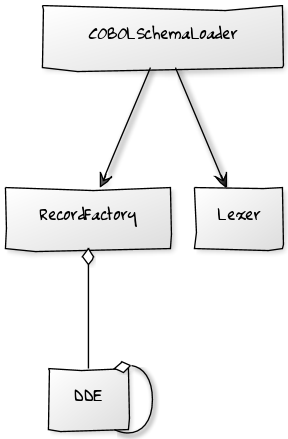
\includegraphics{cobol_final.png}

We have a number of supporting functions that make this work.
\index{make\_attr() (in module cobol.loader)}

\begin{fulllineitems}
\phantomsection\label{cobol_loader:cobol.loader.make_attr}\pysiglinewithargsret{\code{cobol.loader.}\bfcode{make\_attr}}{\emph{aDDE}}{}
Transform a {\hyperref[cobol_defs:cobol.defs.DDE]{\code{cobol.defs.DDE}}} into an  \code{stingray.cobol.RepeatingAttribute}.
This will include a weakref to the DDE so that the source information (like parents and children)
is available. It will also build a weak reference from the original DDE to the resulting
attribute.

\end{fulllineitems}


\begin{Verbatim}[commandchars=\\\{\}]
\PYG{k}{def} \PYG{n+nf}{make\PYGZus{}attr}\PYG{p}{(} \PYG{n}{aDDE} \PYG{p}{)}\PYG{p}{:}
    \PYG{n}{attr}\PYG{o}{=} \PYG{n}{stingray}\PYG{o}{.}\PYG{n}{cobol}\PYG{o}{.}\PYG{n}{RepeatingAttribute}\PYG{p}{(}
        \PYG{c}{\PYGZsh{} Essential features:}
        \PYG{n}{name}\PYG{o}{=} \PYG{n}{aDDE}\PYG{o}{.}\PYG{n}{name}\PYG{p}{,}
        \PYG{n}{size}\PYG{o}{=} \PYG{n}{aDDE}\PYG{o}{.}\PYG{n}{size}\PYG{p}{,}
        \PYG{n}{create}\PYG{o}{=} \PYG{n}{aDDE}\PYG{o}{.}\PYG{n}{usage}\PYG{o}{.}\PYG{n}{create\PYGZus{}func}\PYG{p}{,}

        \PYG{c}{\PYGZsh{} COBOL extensions:}
        \PYG{n}{dde}\PYG{o}{=} \PYG{n}{weakref}\PYG{o}{.}\PYG{n}{ref}\PYG{p}{(}\PYG{n}{aDDE}\PYG{p}{)}\PYG{p}{,}
    \PYG{p}{)}
    \PYG{n}{aDDE}\PYG{o}{.}\PYG{n}{attribute}\PYG{o}{=} \PYG{n}{weakref}\PYG{o}{.}\PYG{n}{ref}\PYG{p}{(} \PYG{n}{attr} \PYG{p}{)}
    \PYG{k}{return} \PYG{n}{attr}
\end{Verbatim}
\index{make\_schema() (in module cobol.loader)}

\begin{fulllineitems}
\phantomsection\label{cobol_loader:cobol.loader.make_schema}\pysiglinewithargsret{\code{cobol.loader.}\bfcode{make\_schema}}{\emph{dde\_iter}}{}
The {\hyperref[schema:schema.Schema]{\code{schema.Schema}}} -- as a whole -- is built by a function
that converts the individual DDE's into attributes.

This may need to be extended in case other DDE names (i.e. paths)
are required in addition to the elementary names.

\end{fulllineitems}


\begin{Verbatim}[commandchars=\\\{\}]
\PYG{k}{def} \PYG{n+nf}{make\PYGZus{}schema}\PYG{p}{(} \PYG{n}{dde\PYGZus{}iter} \PYG{p}{)}\PYG{p}{:}
    \PYG{n}{schema}\PYG{o}{=} \PYG{n}{stingray}\PYG{o}{.}\PYG{n}{schema}\PYG{o}{.}\PYG{n}{Schema}\PYG{p}{(} \PYG{n}{dde}\PYG{o}{=}\PYG{p}{[}\PYG{p}{]} \PYG{p}{)}
    \PYG{k}{for} \PYG{n}{record} \PYG{o+ow}{in} \PYG{n}{dde\PYGZus{}iter}\PYG{p}{:}
        \PYG{n}{schema}\PYG{o}{.}\PYG{n}{info}\PYG{p}{[}\PYG{l+s}{\PYGZsq{}}\PYG{l+s}{dde}\PYG{l+s}{\PYGZsq{}}\PYG{p}{]}\PYG{o}{.}\PYG{n}{append}\PYG{p}{(} \PYG{n}{record} \PYG{p}{)}
        \PYG{k}{for} \PYG{n}{aDDE} \PYG{o+ow}{in} \PYG{n}{record}\PYG{p}{:}
            \PYG{n}{attr}\PYG{o}{=} \PYG{n}{make\PYGZus{}attr}\PYG{p}{(}\PYG{n}{aDDE}\PYG{p}{)}
            \PYG{n}{schema}\PYG{o}{.}\PYG{n}{append}\PYG{p}{(} \PYG{n}{attr} \PYG{p}{)}
    \PYG{k}{return} \PYG{n}{schema}
\end{Verbatim}
\index{COBOLSchemaLoader (class in cobol.loader)}

\begin{fulllineitems}
\phantomsection\label{cobol_loader:cobol.loader.COBOLSchemaLoader}\pysigline{\strong{class }\code{cobol.loader.}\bfcode{COBOLSchemaLoader}}
The overall schema loader process: parse and then build a schema.
This is consistent with the {\hyperref[schema_loader:schema.loader.ExternalSchemaLoader]{\code{schema.loader.ExternalSchemaLoader}}}.

\end{fulllineitems}


\begin{Verbatim}[commandchars=\\\{\}]
\PYG{k}{class} \PYG{n+nc}{COBOLSchemaLoader}\PYG{p}{(} \PYG{n}{stingray}\PYG{o}{.}\PYG{n}{schema}\PYG{o}{.}\PYG{n}{loader}\PYG{o}{.}\PYG{n}{ExternalSchemaLoader} \PYG{p}{)}\PYG{p}{:}
    \PYG{l+s+sd}{\PYGZdq{}\PYGZdq{}\PYGZdq{}Parse a COBOL DDE and create a Schema.}
\PYG{l+s+sd}{    A subclass may define the lexer\PYGZus{}class to customize}
\PYG{l+s+sd}{    parsing.}
\PYG{l+s+sd}{    \PYGZdq{}\PYGZdq{}\PYGZdq{}}
    \PYG{n}{lexer\PYGZus{}class}\PYG{o}{=} \PYG{n}{Lexer}
    \PYG{n}{record\PYGZus{}factory\PYGZus{}class}\PYG{o}{=} \PYG{n}{RecordFactory}
    \PYG{k}{def} \PYG{n+nf}{\PYGZus{}\PYGZus{}init\PYGZus{}\PYGZus{}}\PYG{p}{(} \PYG{n+nb+bp}{self}\PYG{p}{,} \PYG{n}{source}\PYG{p}{,} \PYG{n}{replacing}\PYG{o}{=}\PYG{n+nb+bp}{None} \PYG{p}{)}\PYG{p}{:}
        \PYG{n+nb+bp}{self}\PYG{o}{.}\PYG{n}{source}\PYG{o}{=} \PYG{n}{source}
        \PYG{n+nb+bp}{self}\PYG{o}{.}\PYG{n}{lexer}\PYG{o}{=} \PYG{n+nb+bp}{self}\PYG{o}{.}\PYG{n}{lexer\PYGZus{}class}\PYG{p}{(} \PYG{n}{replacing} \PYG{p}{)}
        \PYG{n+nb+bp}{self}\PYG{o}{.}\PYG{n}{parser}\PYG{o}{=} \PYG{n+nb+bp}{self}\PYG{o}{.}\PYG{n}{record\PYGZus{}factory\PYGZus{}class}\PYG{p}{(}\PYG{p}{)}
\end{Verbatim}
\index{load() (cobol.loader.COBOLSchemaLoader method)}

\begin{fulllineitems}
\phantomsection\label{cobol_loader:cobol.loader.COBOLSchemaLoader.load}\pysiglinewithargsret{\code{COBOLSchemaLoader.}\bfcode{load}}{}{}
Use the {\hyperref[cobol_loader:cobol.loader.RecordFactory.makeRecord]{\code{RecordFactory.makeRecord()}}} method to iterate through
the top-level DDE's. Use {\hyperref[cobol_loader:cobol.loader.make_schema]{\code{make\_schema()}}} to build a single schema
from the DDE(s).

\end{fulllineitems}


\begin{Verbatim}[commandchars=\\\{\}]
\PYG{k}{def} \PYG{n+nf}{load}\PYG{p}{(} \PYG{n+nb+bp}{self} \PYG{p}{)}\PYG{p}{:}
    \PYG{n}{dde\PYGZus{}iter}\PYG{o}{=} \PYG{n+nb+bp}{self}\PYG{o}{.}\PYG{n}{parser}\PYG{o}{.}\PYG{n}{makeRecord}\PYG{p}{(} \PYG{n+nb+bp}{self}\PYG{o}{.}\PYG{n}{lexer}\PYG{o}{.}\PYG{n}{scan}\PYG{p}{(}\PYG{n+nb+bp}{self}\PYG{o}{.}\PYG{n}{source}\PYG{p}{)} \PYG{p}{)}
    \PYG{n}{schema}\PYG{o}{=} \PYG{n}{make\PYGZus{}schema}\PYG{p}{(} \PYG{n}{dde\PYGZus{}iter} \PYG{p}{)}
    \PYG{k}{return} \PYG{n}{schema}
\end{Verbatim}

The \code{replacing} keyword argument is a sequence of pairs: \code{{[} ('old','new'), ...{]}}.
The old text is replaced with the new text.  This seems strange because it is.
COBOL allows replacement text to permit reuse without name clashes.

Note that we provide the ``replacing'' option to the underlying Lexer.
The lexical scanning includes any replacement text.


\paragraph{Top-Level Schema Loader Functions}
\label{cobol_loader:top-level-schema-loader-functions}
The simplest use case is to create an instance of {\hyperref[cobol_loader:cobol.loader.COBOLSchemaLoader]{\code{COBOLSchemaLoader}}}.

\begin{Verbatim}[commandchars=\\\{\}]
\PYG{k}{with} \PYG{n+nb}{open}\PYG{p}{(}\PYG{l+s}{\PYGZdq{}}\PYG{l+s}{sample/zipcty.cob}\PYG{l+s}{\PYGZdq{}}\PYG{p}{,} \PYG{l+s}{\PYGZdq{}}\PYG{l+s}{r}\PYG{l+s}{\PYGZdq{}}\PYG{p}{)} \PYG{k}{as} \PYG{n}{cobol}\PYG{p}{:}
    \PYG{n}{schema}\PYG{o}{=} \PYG{n}{stingray}\PYG{o}{.}\PYG{n}{cobol}\PYG{o}{.}\PYG{n}{loader}\PYG{o}{.}\PYG{n}{COBOLSchemaLoader}\PYG{p}{(} \PYG{n}{cobol} \PYG{p}{)}\PYG{o}{.}\PYG{n}{load}\PYG{p}{(}\PYG{p}{)}
\end{Verbatim}

In some cases, we need to subclass the SchemaLoader to change the lexer.
Here's the example from {\hyperref[cobol_loader:extensions-and-special-cases]{Extensions and Special Cases}}.

\begin{Verbatim}[commandchars=\\\{\}]
\PYG{k}{class} \PYG{n+nc}{MySchemaLoader}\PYG{p}{(} \PYG{n}{cobol}\PYG{o}{.}\PYG{n}{COBOLSchemaLoader} \PYG{p}{)}\PYG{p}{:}
    \PYG{n}{lexer\PYGZus{}class}\PYG{o}{=} \PYG{n}{cobol}\PYG{o}{.}\PYG{n}{loader}\PYG{o}{.}\PYG{n}{Lexer\PYGZus{}Long\PYGZus{}Lines}
\end{Verbatim}

In some cases, we want to see the intermediate COBOL record definitions.
In this case, we want to do something like the following function.
\index{COBOL\_schema() (in module cobol.loader)}

\begin{fulllineitems}
\phantomsection\label{cobol_loader:cobol.loader.COBOL_schema}\pysiglinewithargsret{\code{cobol.loader.}\bfcode{COBOL\_schema}}{\emph{source}, \emph{lexer\_class=Lexer}, \emph{replacing=None}}{}
This function will parse the COBOL copybook, returning a list of the parsed COBOL
01-level records as well as a final schema.

This is based on the (possibly false) assumption
that we're making a single schema object from the definitions provided.
\begin{itemize}
\item {} 
In some cases, we want everything merged into a single schema.

\item {} 
In some edge cases, we want each 01-level to provide a distinct
schema object.

\end{itemize}

We may need to revise this function because we need a different lexer.
We might have some awful formatting issue with the source that needs to be
tweaked.
\begin{quote}\begin{description}
\item[{Parameters}] \leavevmode\begin{itemize}
\item {} 
\textbf{source} -- file-like object that is the open source file.

\item {} 
\textbf{lexer\_class} -- Lexer to use. The default is \code{cobol.load.Lexer}.

\item {} 
\textbf{replacing} -- replacing argument to provide to the lexer.
This is \code{None} by default.

\end{itemize}

\item[{Returns}] \leavevmode
2-tuple (dde\_list, schema).
The first item is a list of 01-level \code{cobol.def.DDE} objects.
The second item is a \code{cobol.defs.Schema} object.

\end{description}\end{quote}

\end{fulllineitems}


\begin{Verbatim}[commandchars=\\\{\}]
\PYG{k}{def} \PYG{n+nf}{COBOL\PYGZus{}schema}\PYG{p}{(} \PYG{n}{source}\PYG{p}{,} \PYG{n}{lexer\PYGZus{}class}\PYG{o}{=}\PYG{n}{Lexer}\PYG{p}{,} \PYG{n}{replacing}\PYG{o}{=}\PYG{n+nb+bp}{None}\PYG{p}{,}  \PYG{p}{)}\PYG{p}{:}
    \PYG{n}{lexer}\PYG{o}{=} \PYG{n}{lexer\PYGZus{}class}\PYG{p}{(} \PYG{n}{replacing} \PYG{p}{)}
    \PYG{n}{parser}\PYG{o}{=} \PYG{n}{RecordFactory}\PYG{p}{(}\PYG{p}{)}
    \PYG{n}{dde\PYGZus{}list}\PYG{o}{=} \PYG{n+nb}{list}\PYG{p}{(} \PYG{n}{parser}\PYG{o}{.}\PYG{n}{makeRecord}\PYG{p}{(} \PYG{n}{lexer}\PYG{o}{.}\PYG{n}{scan}\PYG{p}{(}\PYG{n}{source}\PYG{p}{)} \PYG{p}{)} \PYG{p}{)}
    \PYG{n}{schema}\PYG{o}{=} \PYG{n}{make\PYGZus{}schema}\PYG{p}{(} \PYG{n}{dde\PYGZus{}list} \PYG{p}{)}
    \PYG{k}{return} \PYG{n}{dde\PYGZus{}list}\PYG{p}{,} \PYG{n}{schema}
\end{Verbatim}
\index{COBOL\_schemata() (in module cobol.loader)}

\begin{fulllineitems}
\phantomsection\label{cobol_loader:cobol.loader.COBOL_schemata}\pysiglinewithargsret{\code{cobol.loader.}\bfcode{COBOL\_schemata}}{\emph{source}, \emph{replacing=None}}{}
This function will parse the COBOL copybook, returning two lists:
\begin{itemize}
\item {} 
a list of the parsed COBOL 01-level records, and

\item {} 
a list of final schemata, one for each 01-level definition.

\end{itemize}

This is a peculiar extension in the rare case that we have multiple 01-levels
in a single file and we don't want to (or can't) use them as a single schema.
\begin{quote}\begin{description}
\item[{Parameters}] \leavevmode\begin{itemize}
\item {} 
\textbf{source} -- file-like object that is the open source file.

\item {} 
\textbf{lexer\_class} -- Lexer to use. The default is \code{cobol.load.Lexer}.

\item {} 
\textbf{replacing} -- replacing argument to provide to the lexer.
This is \code{None} by default.

\end{itemize}

\item[{Returns}] \leavevmode
2-tuple (dde\_list, schema).
The first item is a list of 01-level \code{cobol.def.DDE} objects.
The second item is list of \code{cobol.defs.Schema} objects, one for
each 01-level DDE.

\end{description}\end{quote}

\end{fulllineitems}


\begin{Verbatim}[commandchars=\\\{\}]
\PYG{k}{def} \PYG{n+nf}{COBOL\PYGZus{}schemata}\PYG{p}{(} \PYG{n}{source}\PYG{p}{,} \PYG{n}{replacing}\PYG{o}{=}\PYG{n+nb+bp}{None}\PYG{p}{,} \PYG{n}{lexer\PYGZus{}class}\PYG{o}{=}\PYG{n}{Lexer} \PYG{p}{)}\PYG{p}{:}
    \PYG{n}{lexer}\PYG{o}{=} \PYG{n}{lexer\PYGZus{}class}\PYG{p}{(} \PYG{n}{replacing} \PYG{p}{)}
    \PYG{n}{parser}\PYG{o}{=} \PYG{n}{RecordFactory}\PYG{p}{(}\PYG{p}{)}
    \PYG{n}{dde\PYGZus{}list}\PYG{o}{=} \PYG{n+nb}{list}\PYG{p}{(} \PYG{n}{parser}\PYG{o}{.}\PYG{n}{makeRecord}\PYG{p}{(} \PYG{n}{lexer}\PYG{o}{.}\PYG{n}{scan}\PYG{p}{(}\PYG{n}{source}\PYG{p}{)} \PYG{p}{)} \PYG{p}{)}
    \PYG{n}{schema\PYGZus{}list}\PYG{o}{=} \PYG{n+nb}{list}\PYG{p}{(} \PYG{n}{make\PYGZus{}schema}\PYG{p}{(} \PYG{n}{dde} \PYG{p}{)} \PYG{k}{for} \PYG{n}{dde} \PYG{o+ow}{in} \PYG{n}{dde\PYGZus{}list} \PYG{p}{)}
    \PYG{k}{return} \PYG{n}{dde\PYGZus{}list}\PYG{p}{,} \PYG{n}{schema\PYGZus{}list}
\end{Verbatim}

This function gives us two API alternatives for parsing super-complex copybooks.

There's a ``Low-Level API'' that looks like this:

There's a ``High-Level API'' that looks like this:

When opening the workbook, one of the schema must be chosen as the ``official'' schema.


\subsubsection{COBOL Definitions Module -- Handle COBOL DDE's}
\label{cobol_defs:module-cobol.defs}\label{cobol_defs:cobol-defs}\label{cobol_defs:cobol-definitions-module-handle-cobol-dde-s}\label{cobol_defs::doc}\index{cobol.defs (module)}
This is a small set of class definitions and functions
that are used by {\hyperref[cobol_loader:module-cobol.loader]{\code{cobol.loader}}} as well as
{\hyperref[cobol_init:module-cobol]{\code{cobol}}}.

The intent of this module is to avoid a few circular import dependencies.


\paragraph{The Architecture Problem}
\label{cobol_defs:the-architecture-problem}
We have an issue of separation of three concerns:
\begin{itemize}
\item {} 
The underlying workbook and the parsing of CSV or XML or EBCDIC.
This is the Physical Format.

\item {} 
The logical layout or schema we're imposing on the workbook's data.

\item {} 
The process of loading a schema, possibly using a meta-workbook.
This includes the translation of COBOL notation into a useful schema.

\end{itemize}

Except for COBOL, a schema depends on a meta-workbook via a schema loader.
But this is the limit of the relationship. We could say
\begin{gather}
\begin{split}S = L(w)\end{split}\notag
\end{gather}
Or \code{schema= loader(workbook)}. This may involve a separate workbook file,
a separate sheet within a file or even just columns within
the current sheet.

For COBOL, we'd like to keep schema, schema loader and workbook separate, also,
even though COBOL code doesn't depend on COBOL data files.
We'd still like to say \code{schema= loader(cobol source)}.
\begin{gather}
\begin{split}S = L(c)\end{split}\notag
\end{gather}
We can imagine that an application will import a workbook class and a schema loader class.
It will load the schema, then open the workbook using the schema.

\textbf{However}.

A COBOL schema with an occurs depending on (i.e. a DDE with \code{variably\_located == True})
will have the schema depending on each row in addition to the overall loading.

We're really taking about a Baseline Schema, \(S_b\), and a Row-Level Schema, \(S_r\),
that is built by resolving any Occurs Depending On
\begin{gather}
\begin{split}S_b = L(c)\end{split}\notag
\end{gather}\begin{gather}
\begin{split}s_r = R( d, S_b )\end{split}\notag
\end{gather}
We've changed \code{schema\_baseline= loader(cobol source)} and then,
for each row, \code{schema\_row= setSizeAndOffset(data, schema\_baseline)}.


\subparagraph{Where To Recompute}
\label{cobol_defs:where-to-recompute}
The fundamental issue is this: when can we recompute the offsets?

The choices for computing the offsets are these:
\begin{itemize}
\item {} 
At \code{COBOL\_File.rows\_of()} time -- eagerly, but in the wrong module.
See below.

\item {} 
At \code{COBOL\_File.row\_get()} time -- a bit more lazy, but still in the wrong
module, since it's here, not in {\hyperref[cobol_loader:module-cobol.loader]{\code{cobol.loader}}}.

\item {} 
In the application before doing any schema processing on a given row. Very lazy.
But now the application must be more deeply involved in ODO processing. The application
would do something like the following. Sadly, it has a line that's easy to overlook.

\end{itemize}
\begin{alltt}
with open(``xyzzy.cob'') as source:
    dde\_list, schema = COBOL\_schema( source )
with stingray.cobol.Character\_File( filename, schema=schema ) as wb:
    sheet= wb.sheet( filename )
    for row in sheet.rows():
        \textbf{cobol.loader.setSizeAndOffset( dde\_list{[}0{]} )}
        dump( schema, row )
\end{alltt}


\subparagraph{The Module Dependency Problem}
\label{cobol_defs:the-module-dependency-problem}
The {\hyperref[cobol_defs:cobol.defs.Usage]{\code{Usage}}} class properly depends on {\hyperref[cobol_init:module-cobol]{\code{cobol}}}.
The {\hyperref[cobol_loader:cobol.loader.make_attr]{\code{cobol.loader.make\_attr()}}} function, also, properly depends on {\hyperref[cobol_init:module-cobol]{\code{cobol}}}.

The idea is that workbooks are more fundamental than schema. We might need to use
one workbook to build a schema to read another workbook. Schema are higher-level constructs.

We want to avoid any circular dependency between {\hyperref[cobol_loader:module-cobol.loader]{\code{cobol.loader}}} referring
back to {\hyperref[cobol_init:module-cobol]{\code{cobol}}}.
The \code{schema.RepeatingAttribute} definition has a weak version of this undesirable.
dependency.  We finesse it
by defining a bunch of properties that exploit the underlying DDE details without
an explicit \code{import} of the DDE class.

To assure that \code{cobol} does not depend on \code{cobol.loader},
we'd have the class  \code{schema.RepeatingAttribute} entirely built without
reference to the base DDE.
This, however, means that we would effectively clone
the hierarchical relationships into the \code{schema.RepeatingAttribute} objects.
Why bother?

If we extend \code{COBOL\_File.rows\_of()} or \code{COBOL\_File.row\_get()}, we
exacerbates the problem because it would introduce a circular \code{import}. This
would make \code{cobol} depend on \code{cobol.loader} explicitly.


\subparagraph{Resolution}
\label{cobol_defs:resolution}
The \code{setSizeAndOffset()} function as well as a few other
post-processing functions belong in an intermediate module that both \code{cobol}
and \code{cobol.loader} depend on.

Specifically, Cell definitions, DDE definitions, and the related functions required
to build schema attributes from DDE's.

That way, \code{cobol} can import \code{cobol.defs.setSizeAndOffset}.

Also, \code{cobol.loader} can import \code{cobol.defs.DDE}.

And \code{cobol.RepeatingAttribute} can depend on \code{cobol.defs.DDE}.


\paragraph{Overheads}
\label{cobol_defs:overheads}
\begin{Verbatim}[commandchars=\\\{\}]
\PYG{l+s+sd}{\PYGZdq{}\PYGZdq{}\PYGZdq{}stingray.cobol.defs \PYGZhy{}\PYGZhy{} COBOL DDE and Tools.\PYGZdq{}\PYGZdq{}\PYGZdq{}}
\PYG{k+kn}{import} \PYG{n+nn}{logging}
\PYG{k+kn}{import} \PYG{n+nn}{weakref}
\PYG{k+kn}{import} \PYG{n+nn}{warnings}

\PYG{k+kn}{import} \PYG{n+nn}{stingray.cell}
\end{Verbatim}

A module-level logger.

\begin{Verbatim}[commandchars=\\\{\}]
\PYG{n}{logger}\PYG{o}{=} \PYG{n}{logging}\PYG{o}{.}\PYG{n}{getLogger}\PYG{p}{(} \PYG{n}{\PYGZus{}\PYGZus{}name\PYGZus{}\PYGZus{}} \PYG{p}{)}
\end{Verbatim}


\paragraph{Exception}
\label{cobol_defs:exception}\index{UnsupportedError (class in cobol.defs)}

\begin{fulllineitems}
\phantomsection\label{cobol_defs:cobol.defs.UnsupportedError}\pysigline{\strong{class }\code{cobol.defs.}\bfcode{UnsupportedError}}
A syntax which expresses an unsupported feature
of the COBOL language.

\end{fulllineitems}


\begin{Verbatim}[commandchars=\\\{\}]
\PYG{k}{class} \PYG{n+nc}{UnsupportedError}\PYG{p}{(} \PYG{n+ne}{Exception} \PYG{p}{)}\PYG{p}{:}
    \PYG{l+s+sd}{\PYGZdq{}\PYGZdq{}\PYGZdq{}A COBOL DDE has features not supported by this module.\PYGZdq{}\PYGZdq{}\PYGZdq{}}
    \PYG{k}{pass}
\end{Verbatim}

The most important unsupported feature may be ``separate signs.''  These may be
required for decoding bytes in some files.


\paragraph{Cell Subclasses and Conversions}
\label{cobol_defs:cell-subclasses-and-conversions}
Rather than tinker too much with the {\hyperref[cell:module-cell]{\code{cell}}} module,
it seems better to introduce new {\hyperref[cell:cell.Cell]{\code{cell.Cell}}} subclasses unique to COBOL, EBCIDC
and COMP-3 data.

There are three relevant features.
\begin{itemize}
\item {} 
Proper conversion from source characters or bytes.

\item {} 
Preservation of the source characters (or bytes) for creating
character-level (or byte-level) structured dumps of a record.

\item {} 
Preservation of the original DDE attributes, because there is so much
information required to interpret the bytes.

\end{itemize}

Consequently, even the {\hyperref[cell:cell.TextCell]{\code{cell.TextCell}}} must be extended to include
preservation of raw data.

Further, we have a distinction between text and numbers which are
``USAGE DISPLAY''.

\begin{Verbatim}[commandchars=\\\{\}]
http://yuml.me/diagram/scruffy;/class/
\PYGZsh{}cobol.cell,
[TextCell]\PYGZca{}[NumberCell],
[NumberCell]\PYGZca{}[NumberDisplayCell],
[NumberCell]\PYGZca{}[NumberCompCell],
[NumberCell]\PYGZca{}[NumberComp3Cell],
[TextCell]\PYGZca{}[ErrorCell],
\end{Verbatim}

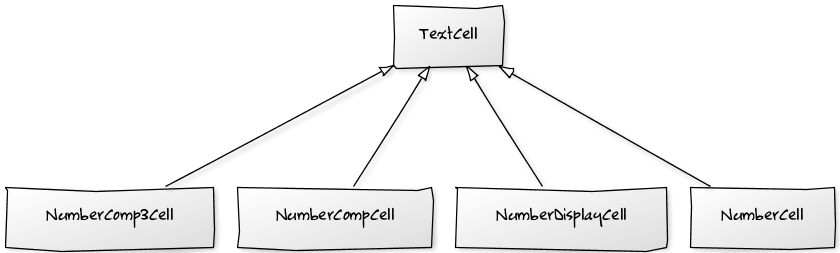
\includegraphics[width=6in]{cobol_cell.png}

\begin{notice}{warning}{Warning:}
Non-Polymorphic.

These classes are profound extensions to the base definitions of {\hyperref[cell:module-cell]{\code{cell}}}.
They are not polymorphic with the base classes.
COBOL processing is not transparently identical to other workbook processing.
\end{notice}

These cells are conventionally built by the the {\hyperref[cobol_init:cobol.COBOL_File]{\code{cobol.COBOL\_File}}} version
of Workbook as a factory. These are rarely built any other way.
\index{TextCell (class in cobol.defs)}

\begin{fulllineitems}
\phantomsection\label{cobol_defs:cobol.defs.TextCell}\pysigline{\strong{class }\code{cobol.defs.}\bfcode{TextCell}}
A cell which contains COBOL Alphanumeric data.

\end{fulllineitems}


\begin{Verbatim}[commandchars=\\\{\}]
\PYG{k}{class} \PYG{n+nc}{TextCell}\PYG{p}{(} \PYG{n}{stingray}\PYG{o}{.}\PYG{n}{cell}\PYG{o}{.}\PYG{n}{TextCell} \PYG{p}{)}\PYG{p}{:}
    \PYG{l+s+sd}{\PYGZdq{}\PYGZdq{}\PYGZdq{}A COBOL TextCell, usually Usage Display.\PYGZdq{}\PYGZdq{}\PYGZdq{}}
    \PYG{k}{def} \PYG{n+nf}{\PYGZus{}\PYGZus{}init\PYGZus{}\PYGZus{}}\PYG{p}{(} \PYG{n+nb+bp}{self}\PYG{p}{,} \PYG{n}{raw}\PYG{p}{,} \PYG{n}{workbook}\PYG{p}{,} \PYG{n}{attr} \PYG{p}{)}\PYG{p}{:}
        \PYG{n+nb+bp}{self}\PYG{o}{.}\PYG{n}{raw}\PYG{p}{,} \PYG{n+nb+bp}{self}\PYG{o}{.}\PYG{n}{workbook}\PYG{o}{=} \PYG{n}{raw}\PYG{p}{,} \PYG{n}{workbook}
        \PYG{n+nb+bp}{self}\PYG{o}{.}\PYG{n}{\PYGZus{}value}\PYG{o}{=} \PYG{n}{workbook}\PYG{o}{.}\PYG{n}{text}\PYG{p}{(} \PYG{n+nb+bp}{self}\PYG{o}{.}\PYG{n}{raw}\PYG{p}{,} \PYG{n}{attr} \PYG{p}{)}
\end{Verbatim}
\index{NumberCell (class in cobol.defs)}

\begin{fulllineitems}
\phantomsection\label{cobol_defs:cobol.defs.NumberCell}\pysigline{\strong{class }\code{cobol.defs.}\bfcode{NumberCell}}
This is an abstraction to simply hold all the standard conversions

\end{fulllineitems}


\begin{Verbatim}[commandchars=\\\{\}]
\PYG{k}{class} \PYG{n+nc}{NumberCell}\PYG{p}{(} \PYG{n}{stingray}\PYG{o}{.}\PYG{n}{cell}\PYG{o}{.}\PYG{n}{NumberCell} \PYG{p}{)}\PYG{p}{:}
    \PYG{l+s+sd}{\PYGZdq{}\PYGZdq{}\PYGZdq{}A COBOL number.\PYGZdq{}\PYGZdq{}\PYGZdq{}}
    \PYG{k}{def} \PYG{n+nf}{to\PYGZus{}int}\PYG{p}{(} \PYG{n+nb+bp}{self} \PYG{p}{)}\PYG{p}{:} \PYG{k}{return} \PYG{n+nb}{int}\PYG{p}{(}\PYG{n+nb+bp}{self}\PYG{o}{.}\PYG{n}{value}\PYG{p}{)}
    \PYG{k}{def} \PYG{n+nf}{to\PYGZus{}float}\PYG{p}{(} \PYG{n+nb+bp}{self} \PYG{p}{)}\PYG{p}{:} \PYG{k}{return} \PYG{n+nb}{float}\PYG{p}{(}\PYG{n+nb+bp}{self}\PYG{o}{.}\PYG{n}{value}\PYG{p}{)}
    \PYG{k}{def} \PYG{n+nf}{to\PYGZus{}decimal}\PYG{p}{(} \PYG{n+nb+bp}{self}\PYG{p}{,} \PYG{n}{digits}\PYG{o}{=}\PYG{n+nb+bp}{None} \PYG{p}{)}\PYG{p}{:} \PYG{k}{return} \PYG{n+nb+bp}{self}\PYG{o}{.}\PYG{n}{value}
    \PYG{k}{def} \PYG{n+nf}{to\PYGZus{}str}\PYG{p}{(} \PYG{n+nb+bp}{self} \PYG{p}{)}\PYG{p}{:} \PYG{k}{return} \PYG{n+nb}{str}\PYG{p}{(}\PYG{n+nb+bp}{self}\PYG{o}{.}\PYG{n}{value}\PYG{p}{)}
\end{Verbatim}
\index{NumberDisplayCell (class in cobol.defs)}

\begin{fulllineitems}
\phantomsection\label{cobol_defs:cobol.defs.NumberDisplayCell}\pysigline{\strong{class }\code{cobol.defs.}\bfcode{NumberDisplayCell}}
A COBOL numeric item with USAGE DISPLAY.

\end{fulllineitems}


\begin{Verbatim}[commandchars=\\\{\}]
\PYG{k}{class} \PYG{n+nc}{NumberDisplayCell}\PYG{p}{(} \PYG{n}{NumberCell} \PYG{p}{)}\PYG{p}{:}
    \PYG{l+s+sd}{\PYGZdq{}\PYGZdq{}\PYGZdq{}A COBOL Usage Display Numeric Cell.\PYGZdq{}\PYGZdq{}\PYGZdq{}}
    \PYG{k}{def} \PYG{n+nf}{\PYGZus{}\PYGZus{}init\PYGZus{}\PYGZus{}}\PYG{p}{(} \PYG{n+nb+bp}{self}\PYG{p}{,} \PYG{n}{raw}\PYG{p}{,} \PYG{n}{workbook}\PYG{p}{,} \PYG{n}{attr} \PYG{p}{)}\PYG{p}{:}
        \PYG{n+nb+bp}{self}\PYG{o}{.}\PYG{n}{raw}\PYG{p}{,} \PYG{n+nb+bp}{self}\PYG{o}{.}\PYG{n}{workbook}\PYG{o}{=} \PYG{n}{raw}\PYG{p}{,} \PYG{n}{workbook}
        \PYG{n+nb+bp}{self}\PYG{o}{.}\PYG{n}{\PYGZus{}value}\PYG{o}{=} \PYG{n}{workbook}\PYG{o}{.}\PYG{n}{number\PYGZus{}display}\PYG{p}{(} \PYG{n+nb+bp}{self}\PYG{o}{.}\PYG{n}{raw}\PYG{p}{,} \PYG{n}{attr} \PYG{p}{)}
\end{Verbatim}
\index{NumberCompCell (class in cobol.defs)}

\begin{fulllineitems}
\phantomsection\label{cobol_defs:cobol.defs.NumberCompCell}\pysigline{\strong{class }\code{cobol.defs.}\bfcode{NumberCompCell}}
A COBOL numeric item with USAGE COMPUTATIONAL.

\end{fulllineitems}


\begin{Verbatim}[commandchars=\\\{\}]
\PYG{k}{class} \PYG{n+nc}{NumberCompCell}\PYG{p}{(} \PYG{n}{NumberCell} \PYG{p}{)}\PYG{p}{:}
    \PYG{l+s+sd}{\PYGZdq{}\PYGZdq{}\PYGZdq{}A COBOL Usage COMP Numeric Cell.}
\PYG{l+s+sd}{    Three formats.  Half\PYGZhy{}word, whole\PYGZhy{}word and double\PYGZhy{}word.}
\PYG{l+s+sd}{    \PYGZdq{}\PYGZdq{}\PYGZdq{}}
    \PYG{k}{def} \PYG{n+nf}{\PYGZus{}\PYGZus{}init\PYGZus{}\PYGZus{}}\PYG{p}{(} \PYG{n+nb+bp}{self}\PYG{p}{,} \PYG{n}{raw}\PYG{p}{,} \PYG{n}{workbook}\PYG{p}{,} \PYG{n}{attr} \PYG{p}{)}\PYG{p}{:}
        \PYG{n+nb+bp}{self}\PYG{o}{.}\PYG{n}{raw}\PYG{p}{,} \PYG{n+nb+bp}{self}\PYG{o}{.}\PYG{n}{workbook}\PYG{o}{=} \PYG{n}{raw}\PYG{p}{,} \PYG{n}{workbook}
        \PYG{n+nb+bp}{self}\PYG{o}{.}\PYG{n}{\PYGZus{}value}\PYG{o}{=} \PYG{n}{workbook}\PYG{o}{.}\PYG{n}{number\PYGZus{}comp}\PYG{p}{(} \PYG{n+nb+bp}{self}\PYG{o}{.}\PYG{n}{raw}\PYG{p}{,} \PYG{n}{attr} \PYG{p}{)}
\end{Verbatim}
\index{NumberComp3Cell (class in cobol.defs)}

\begin{fulllineitems}
\phantomsection\label{cobol_defs:cobol.defs.NumberComp3Cell}\pysigline{\strong{class }\code{cobol.defs.}\bfcode{NumberComp3Cell}}
A COBOL numeric item with USAGE COMPUTATIONAL-3.

\end{fulllineitems}


\begin{Verbatim}[commandchars=\\\{\}]
\PYG{k}{class} \PYG{n+nc}{NumberComp3Cell}\PYG{p}{(} \PYG{n}{NumberCell} \PYG{p}{)}\PYG{p}{:}
    \PYG{l+s+sd}{\PYGZdq{}\PYGZdq{}\PYGZdq{}A COBOL Usage COMP\PYGZhy{}3 Numeric Cell..\PYGZdq{}\PYGZdq{}\PYGZdq{}}
    \PYG{k}{def} \PYG{n+nf}{\PYGZus{}\PYGZus{}init\PYGZus{}\PYGZus{}}\PYG{p}{(} \PYG{n+nb+bp}{self}\PYG{p}{,} \PYG{n}{raw}\PYG{p}{,} \PYG{n}{workbook}\PYG{p}{,} \PYG{n}{attr} \PYG{p}{)}\PYG{p}{:}
        \PYG{n+nb+bp}{self}\PYG{o}{.}\PYG{n}{raw}\PYG{p}{,} \PYG{n+nb+bp}{self}\PYG{o}{.}\PYG{n}{workbook}\PYG{o}{=} \PYG{n}{raw}\PYG{p}{,} \PYG{n}{workbook}
        \PYG{n+nb+bp}{self}\PYG{o}{.}\PYG{n}{\PYGZus{}value}\PYG{o}{=} \PYG{n}{workbook}\PYG{o}{.}\PYG{n}{number\PYGZus{}comp3}\PYG{p}{(} \PYG{n+nb+bp}{self}\PYG{o}{.}\PYG{n}{raw}\PYG{p}{,} \PYG{n}{attr} \PYG{p}{)}
\end{Verbatim}
\index{ErrorCell (class in cobol.defs)}

\begin{fulllineitems}
\phantomsection\label{cobol_defs:cobol.defs.ErrorCell}\pysigline{\strong{class }\code{cobol.defs.}\bfcode{ErrorCell}}
A COBOL numeric item with invalid data.

\end{fulllineitems}


\begin{Verbatim}[commandchars=\\\{\}]
\PYG{k}{class} \PYG{n+nc}{ErrorCell}\PYG{p}{(} \PYG{n}{stingray}\PYG{o}{.}\PYG{n}{cell}\PYG{o}{.}\PYG{n}{ErrorCell} \PYG{p}{)}\PYG{p}{:}
    \PYG{l+s+sd}{\PYGZdq{}\PYGZdq{}\PYGZdq{}A COBOL ErrorCell, bad data bytes with no relevant value.\PYGZdq{}\PYGZdq{}\PYGZdq{}}
    \PYG{k}{def} \PYG{n+nf}{\PYGZus{}\PYGZus{}init\PYGZus{}\PYGZus{}}\PYG{p}{(} \PYG{n+nb+bp}{self}\PYG{p}{,} \PYG{n}{raw}\PYG{p}{,} \PYG{n}{workbook}\PYG{p}{,} \PYG{n}{attr}\PYG{p}{,} \PYG{n}{exception}\PYG{o}{=}\PYG{n+nb+bp}{None} \PYG{p}{)}\PYG{p}{:}
        \PYG{n+nb+bp}{self}\PYG{o}{.}\PYG{n}{raw}\PYG{p}{,} \PYG{n+nb+bp}{self}\PYG{o}{.}\PYG{n}{workbook}\PYG{o}{=} \PYG{n}{raw}\PYG{p}{,} \PYG{n}{workbook}
        \PYG{n+nb+bp}{self}\PYG{o}{.}\PYG{n}{\PYGZus{}value}\PYG{o}{=} \PYG{n+nb+bp}{None}
        \PYG{n+nb+bp}{self}\PYG{o}{.}\PYG{n}{exception}\PYG{o}{=} \PYG{n}{exception}
    \PYG{k}{def} \PYG{n+nf}{\PYGZus{}\PYGZus{}repr\PYGZus{}\PYGZus{}}\PYG{p}{(} \PYG{n+nb+bp}{self} \PYG{p}{)}\PYG{p}{:}
        \PYG{k}{return} \PYG{l+s}{\PYGZdq{}}\PYG{l+s}{\PYGZob{}0\PYGZcb{}(\PYGZob{}1!r\PYGZcb{}, \PYGZob{}2!r\PYGZcb{})}\PYG{l+s}{\PYGZdq{}}\PYG{o}{.}\PYG{n}{format}\PYG{p}{(}
            \PYG{n+nb+bp}{self}\PYG{o}{.}\PYG{n}{\PYGZus{}\PYGZus{}class\PYGZus{}\PYGZus{}}\PYG{o}{.}\PYG{n}{\PYGZus{}\PYGZus{}name\PYGZus{}\PYGZus{}}\PYG{p}{,} \PYG{n+nb+bp}{self}\PYG{o}{.}\PYG{n}{exception}\PYG{p}{,} \PYG{n+nb+bp}{self}\PYG{o}{.}\PYG{n}{raw} \PYG{p}{)}
\end{Verbatim}


\paragraph{Essential Class Definitions}
\label{cobol_defs:essential-class-definitions}
The essential class definitions define the DDE we're attempting to build.
We can  separated this structure into a few high-level subject areas:
\begin{itemize}
\item {} 
{\hyperref[cobol_defs:usage-strategy-hierarchy]{Usage Strategy Hierarchy}} defines the various
kinds of USAGE options.

\item {} 
{\hyperref[cobol_defs:allocation-strategy-hierarchy]{Allocation Strategy Hierarchy}} defines the relationships among DDE's:
Predecessor/Successor, Group/Elementary or Redefines.

\item {} 
{\hyperref[cobol_defs:occurs-strategy-hierarchy]{Occurs Strategy Hierarchy}} defines the Occurs options of
Default (no Occurs), simple Occurs, and more complex Occurs Depending On.

\item {} 
The {\hyperref[cobol_defs:dde-class]{DDE Class}} itself.

\end{itemize}


\subparagraph{Usage Strategy Hierarchy}
\label{cobol_defs:usage-strategy-hierarchy}
The {\hyperref[cobol_defs:cobol.defs.Usage]{\code{Usage}}} class combines information in the picture, usage, sign and synchronized clauses.

The \textbf{Strategy} design pattern allows a DDE element to delegate
the {\hyperref[cobol_defs:cobol.defs.Usage.size]{\code{Usage.size()}}} and {\hyperref[cobol_defs:cobol.defs.Usage.create_func]{\code{Usage.create\_func()}}} operations to this class.

The {\hyperref[cobol_defs:cobol.defs.Usage.size]{\code{Usage.size()}}} method returns the number
of bytes used by the data element.
\begin{itemize}
\item {} 
For usage \code{DISPLAY}, the size is computed directly from the picture clause.

\item {} 
For usage \code{COMP}, the size is 2, 4 or 8 bytes based on the picture clause.

\item {} 
For usage \code{COMP-3}, the picture clause digits are packed two per byte
with an extra half-byte for sign information. This must be rounded up.
COMP-3 fields often have an odd number of digits to reflect this.

\end{itemize}

The {\hyperref[cobol_defs:cobol.defs.Usage.create_func]{\code{Usage.create\_func()}}} method returns a {\hyperref[cell:cell.Cell]{\code{cell.Cell}}} type
that should be built from the raw bytes.

\begin{Verbatim}[commandchars=\\\{\}]
http://yuml.me/diagram/scruffy;/class/
\PYGZsh{}cobol\PYGZus{}loader\PYGZus{}usage,
[RecordFactory]\PYGZlt{}\PYGZgt{}\PYGZhy{}[DDE],
[DDE]\PYGZlt{}\PYGZgt{}\PYGZhy{}[DDE],
[DDE]\PYGZhy{}[Usage],
[Usage]\PYGZca{}[UsageDisplay],
[Usage]\PYGZca{}[UsageComp]
[Usage]\PYGZca{}[UsageComp3]
\end{Verbatim}

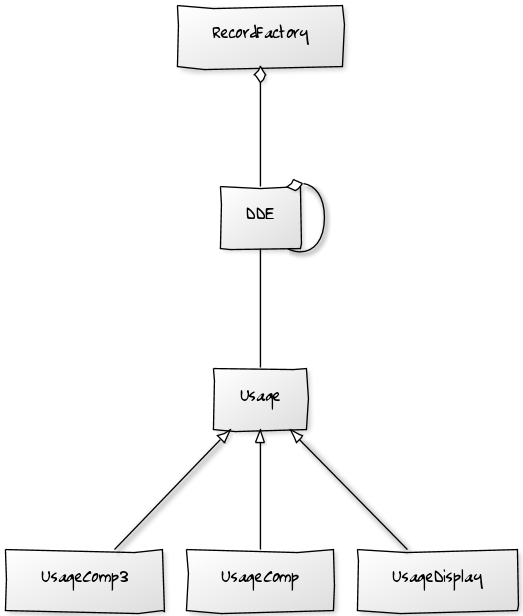
\includegraphics{cobol_usage.png}
\index{Usage (class in cobol.defs)}

\begin{fulllineitems}
\phantomsection\label{cobol_defs:cobol.defs.Usage}\pysigline{\strong{class }\code{cobol.defs.}\bfcode{Usage}}
The Usage class provides detailed representation and conversion support
for a given DDE. A {\hyperref[schema:schema.Attribute]{\code{schema.Attribute}}} will refer to a
{\hyperref[cobol_defs:cobol.defs.DDE]{\code{cobol.defs.DDE}}}. This DDE will have a {\hyperref[cobol_defs:cobol.defs.Usage]{\code{Usage}}} object that shows
how to create the underlying \code{Cell} instance from the raw data
in the {\hyperref[cobol_init:cobol.COBOL_File]{\code{cobol.COBOL\_File}}} subclass of \code{Workbook}.

For numeric types, this may mean a fallback from creating a {\hyperref[cobol_defs:cobol.defs.NumberCell]{\code{NumberCell}}}
to creating a {\hyperref[cobol_defs:cobol.defs.ErrorCell]{\code{ErrorCell}}}. If the number is invalid in some way, then
an error is required.

The superclass of \code{Usage} is abstract and doesn't compute a proper size.

\end{fulllineitems}


\begin{Verbatim}[commandchars=\\\{\}]
\PYG{k}{class} \PYG{n+nc}{Usage}\PYG{p}{:}
    \PYG{l+s+sd}{\PYGZdq{}\PYGZdq{}\PYGZdq{}Covert numeric data based on Usage clause.\PYGZdq{}\PYGZdq{}\PYGZdq{}}
    \PYG{k}{def} \PYG{n+nf}{\PYGZus{}\PYGZus{}init\PYGZus{}\PYGZus{}}\PYG{p}{(} \PYG{n+nb+bp}{self}\PYG{p}{,} \PYG{n}{source} \PYG{p}{)}\PYG{p}{:}
        \PYG{n+nb+bp}{self}\PYG{o}{.}\PYG{n}{source\PYGZus{}}\PYG{o}{=} \PYG{n}{source}
        \PYG{n+nb+bp}{self}\PYG{o}{.}\PYG{n}{final}\PYG{o}{=} \PYG{n}{source}
        \PYG{n+nb+bp}{self}\PYG{o}{.}\PYG{n}{numeric}\PYG{o}{=} \PYG{n+nb+bp}{None} \PYG{c}{\PYGZsh{} is the picture all digits?}
        \PYG{n+nb+bp}{self}\PYG{o}{.}\PYG{n}{length}\PYG{o}{=} \PYG{n+nb+bp}{None}
        \PYG{n+nb+bp}{self}\PYG{o}{.}\PYG{n}{scale}\PYG{o}{=} \PYG{n+nb+bp}{None}
        \PYG{n+nb+bp}{self}\PYG{o}{.}\PYG{n}{precision}\PYG{o}{=} \PYG{n+nb+bp}{None}
        \PYG{n+nb+bp}{self}\PYG{o}{.}\PYG{n}{signed}\PYG{o}{=} \PYG{n+nb+bp}{None}
        \PYG{n+nb+bp}{self}\PYG{o}{.}\PYG{n}{decimal}\PYG{o}{=} \PYG{n+nb+bp}{None}
    \PYG{k}{def} \PYG{n+nf}{setTypeInfo}\PYG{p}{(} \PYG{n+nb+bp}{self}\PYG{p}{,} \PYG{n}{picture} \PYG{p}{)}\PYG{p}{:}
        \PYG{l+s+sd}{\PYGZdq{}\PYGZdq{}\PYGZdq{}Details from parsing a PICTURE clause.\PYGZdq{}\PYGZdq{}\PYGZdq{}}
        \PYG{n+nb+bp}{self}\PYG{o}{.}\PYG{n}{final}\PYG{o}{=} \PYG{n}{picture}\PYG{o}{.}\PYG{n}{final}
        \PYG{n+nb+bp}{self}\PYG{o}{.}\PYG{n}{numeric} \PYG{o}{=} \PYG{o+ow}{not} \PYG{n}{picture}\PYG{o}{.}\PYG{n}{alpha}
        \PYG{n+nb+bp}{self}\PYG{o}{.}\PYG{n}{length} \PYG{o}{=} \PYG{n}{picture}\PYG{o}{.}\PYG{n}{length}
        \PYG{n+nb+bp}{self}\PYG{o}{.}\PYG{n}{scale} \PYG{o}{=} \PYG{n}{picture}\PYG{o}{.}\PYG{n}{scale}
        \PYG{n+nb+bp}{self}\PYG{o}{.}\PYG{n}{precision} \PYG{o}{=} \PYG{n}{picture}\PYG{o}{.}\PYG{n}{precision}
        \PYG{n+nb+bp}{self}\PYG{o}{.}\PYG{n}{signed} \PYG{o}{=} \PYG{n}{picture}\PYG{o}{.}\PYG{n}{signed}
        \PYG{n+nb+bp}{self}\PYG{o}{.}\PYG{n}{decimal} \PYG{o}{=} \PYG{n}{picture}\PYG{o}{.}\PYG{n}{decimal}
    \PYG{k}{def} \PYG{n+nf}{source}\PYG{p}{(} \PYG{n+nb+bp}{self} \PYG{p}{)}\PYG{p}{:}
        \PYG{k}{return} \PYG{n+nb+bp}{self}\PYG{o}{.}\PYG{n}{source\PYGZus{}}
\end{Verbatim}
\index{create\_func() (cobol.defs.Usage method)}

\begin{fulllineitems}
\phantomsection\label{cobol_defs:cobol.defs.Usage.create_func}\pysiglinewithargsret{\code{Usage.}\bfcode{create\_func}}{}{}
Create a CELL object. Use the raw bytes to build an Cell described
by the given Attribute.

\end{fulllineitems}


\begin{Verbatim}[commandchars=\\\{\}]
\PYG{k}{def} \PYG{n+nf}{create\PYGZus{}func}\PYG{p}{(} \PYG{n+nb+bp}{self}\PYG{p}{,} \PYG{n}{raw}\PYG{p}{,} \PYG{n}{workbook}\PYG{p}{,} \PYG{n}{attr} \PYG{p}{)}\PYG{p}{:}
    \PYG{l+s+sd}{\PYGZdq{}\PYGZdq{}\PYGZdq{}Converts bytes to a proper Cell object.}
\PYG{l+s+sd}{    NOTE: EBCDIC\PYGZhy{}\PYGZgt{}ASCII conversion handled by the Workbook object.}
\PYG{l+s+sd}{    \PYGZdq{}\PYGZdq{}\PYGZdq{}}
    \PYG{k}{return} \PYG{n}{stingray}\PYG{o}{.}\PYG{n}{cobol}\PYG{o}{.}\PYG{n}{TextCell}\PYG{p}{(} \PYG{n}{raw}\PYG{p}{,} \PYG{n}{workbook}\PYG{p}{,} \PYG{n}{attr} \PYG{p}{)}
\end{Verbatim}
\index{size() (cobol.defs.Usage method)}

\begin{fulllineitems}
\phantomsection\label{cobol_defs:cobol.defs.Usage.size}\pysiglinewithargsret{\code{Usage.}\bfcode{size}}{\emph{picture}}{}
The count is in bytes.  Not characters.

\end{fulllineitems}


\begin{Verbatim}[commandchars=\\\{\}]
\PYG{k}{def} \PYG{n+nf}{size}\PYG{p}{(} \PYG{n+nb+bp}{self}\PYG{p}{,} \PYG{n}{picture} \PYG{p}{)}\PYG{p}{:}
    \PYG{l+s+sd}{\PYGZdq{}\PYGZdq{}\PYGZdq{}Default for group\PYGZhy{}level items.\PYGZdq{}\PYGZdq{}\PYGZdq{}}
    \PYG{k}{return} \PYG{l+m+mi}{0}
\end{Verbatim}
\index{UsageDisplay (class in cobol.defs)}

\begin{fulllineitems}
\phantomsection\label{cobol_defs:cobol.defs.UsageDisplay}\pysigline{\strong{class }\code{cobol.defs.}\bfcode{UsageDisplay}}
Usage ``DISPLAY'' is the COBOL language default.  It's also assumed for group-level items.

\end{fulllineitems}


\begin{Verbatim}[commandchars=\\\{\}]
\PYG{k}{class} \PYG{n+nc}{UsageDisplay}\PYG{p}{(} \PYG{n}{Usage} \PYG{p}{)}\PYG{p}{:}
    \PYG{l+s+sd}{\PYGZdq{}\PYGZdq{}\PYGZdq{}Ordinary character data which is numeric.\PYGZdq{}\PYGZdq{}\PYGZdq{}}
    \PYG{k}{def} \PYG{n+nf}{\PYGZus{}\PYGZus{}init\PYGZus{}\PYGZus{}}\PYG{p}{(} \PYG{n+nb+bp}{self}\PYG{p}{,} \PYG{n}{source} \PYG{p}{)}\PYG{p}{:}
        \PYG{n+nb}{super}\PYG{p}{(}\PYG{p}{)}\PYG{o}{.}\PYG{n}{\PYGZus{}\PYGZus{}init\PYGZus{}\PYGZus{}}\PYG{p}{(} \PYG{n}{source} \PYG{p}{)}
    \PYG{k}{def} \PYG{n+nf}{create\PYGZus{}func}\PYG{p}{(} \PYG{n+nb+bp}{self}\PYG{p}{,} \PYG{n}{raw}\PYG{p}{,} \PYG{n}{workbook}\PYG{p}{,} \PYG{n}{attr} \PYG{p}{)}\PYG{p}{:}
        \PYG{k}{if} \PYG{n+nb+bp}{self}\PYG{o}{.}\PYG{n}{numeric}\PYG{p}{:}
            \PYG{k}{try}\PYG{p}{:}
                \PYG{k}{return} \PYG{n}{NumberDisplayCell}\PYG{p}{(} \PYG{n}{raw}\PYG{p}{,} \PYG{n}{workbook}\PYG{p}{,} \PYG{n}{attr} \PYG{p}{)}
            \PYG{k}{except} \PYG{n+ne}{Exception} \PYG{k}{as} \PYG{n}{e}\PYG{p}{:}
                \PYG{n}{error}\PYG{o}{=} \PYG{n}{ErrorCell}\PYG{p}{(} \PYG{n}{raw}\PYG{p}{,} \PYG{n}{workbook}\PYG{p}{,} \PYG{n}{attr}\PYG{p}{,} \PYG{n}{exception}\PYG{o}{=}\PYG{n}{e} \PYG{p}{)}
                \PYG{k}{return} \PYG{n}{error}
        \PYG{k}{return} \PYG{n}{stingray}\PYG{o}{.}\PYG{n}{cobol}\PYG{o}{.}\PYG{n}{TextCell}\PYG{p}{(} \PYG{n}{raw}\PYG{p}{,} \PYG{n}{workbook}\PYG{p}{,} \PYG{n}{attr} \PYG{p}{)}
    \PYG{k}{def} \PYG{n+nf}{size}\PYG{p}{(} \PYG{n+nb+bp}{self} \PYG{p}{)}\PYG{p}{:}
        \PYG{l+s+sd}{\PYGZdq{}\PYGZdq{}\PYGZdq{}Return the actual size of this data, based on PICTURE and SIGN.\PYGZdq{}\PYGZdq{}\PYGZdq{}}
        \PYG{k}{return} \PYG{n+nb}{len}\PYG{p}{(}\PYG{n+nb+bp}{self}\PYG{o}{.}\PYG{n}{final}\PYG{p}{)}
\end{Verbatim}
\index{UsageComp (class in cobol.defs)}

\begin{fulllineitems}
\phantomsection\label{cobol_defs:cobol.defs.UsageComp}\pysigline{\strong{class }\code{cobol.defs.}\bfcode{UsageComp}}
Usage ``COMPUTATIONAL'' is binary-encoded data.

\end{fulllineitems}


\begin{Verbatim}[commandchars=\\\{\}]
\PYG{k}{class} \PYG{n+nc}{UsageComp}\PYG{p}{(} \PYG{n}{Usage} \PYG{p}{)}\PYG{p}{:}
    \PYG{l+s+sd}{\PYGZdq{}\PYGZdq{}\PYGZdq{}Binary\PYGZhy{}encoded COMP data which is numeric.\PYGZdq{}\PYGZdq{}\PYGZdq{}}
    \PYG{k}{def} \PYG{n+nf}{\PYGZus{}\PYGZus{}init\PYGZus{}\PYGZus{}}\PYG{p}{(} \PYG{n+nb+bp}{self}\PYG{p}{,} \PYG{n}{source} \PYG{p}{)}\PYG{p}{:}
        \PYG{n+nb}{super}\PYG{p}{(}\PYG{p}{)}\PYG{o}{.}\PYG{n}{\PYGZus{}\PYGZus{}init\PYGZus{}\PYGZus{}}\PYG{p}{(} \PYG{n}{source} \PYG{p}{)}
    \PYG{k}{def} \PYG{n+nf}{create\PYGZus{}func}\PYG{p}{(} \PYG{n+nb+bp}{self}\PYG{p}{,} \PYG{n}{raw}\PYG{p}{,} \PYG{n}{workbook}\PYG{p}{,} \PYG{n}{attr} \PYG{p}{)}\PYG{p}{:}
        \PYG{k}{try}\PYG{p}{:}
            \PYG{k}{return} \PYG{n}{NumberCompCell}\PYG{p}{(} \PYG{n}{raw}\PYG{p}{,} \PYG{n}{workbook}\PYG{p}{,} \PYG{n}{attr} \PYG{p}{)}
        \PYG{k}{except} \PYG{n+ne}{Exception} \PYG{k}{as} \PYG{n}{e}\PYG{p}{:}
            \PYG{n}{error}\PYG{o}{=} \PYG{n}{ErrorCell}\PYG{p}{(} \PYG{n}{raw}\PYG{p}{,} \PYG{n}{workbook}\PYG{p}{,} \PYG{n}{attr}\PYG{p}{,} \PYG{n}{exception}\PYG{o}{=}\PYG{n}{e} \PYG{p}{)}
            \PYG{k}{return} \PYG{n}{error}
    \PYG{k}{def} \PYG{n+nf}{size}\PYG{p}{(} \PYG{n+nb+bp}{self} \PYG{p}{)}\PYG{p}{:}
        \PYG{l+s+sd}{\PYGZdq{}\PYGZdq{}\PYGZdq{}COMP is binary half word, whole word or double word.\PYGZdq{}\PYGZdq{}\PYGZdq{}}
        \PYG{k}{if} \PYG{n+nb}{len}\PYG{p}{(}\PYG{n+nb+bp}{self}\PYG{o}{.}\PYG{n}{final}\PYG{p}{)} \PYG{o}{\PYGZlt{}}\PYG{o}{=} \PYG{l+m+mi}{4}\PYG{p}{:}
            \PYG{k}{return} \PYG{l+m+mi}{2}
        \PYG{k}{elif} \PYG{n+nb}{len}\PYG{p}{(}\PYG{n+nb+bp}{self}\PYG{o}{.}\PYG{n}{final}\PYG{p}{)} \PYG{o}{\PYGZlt{}}\PYG{o}{=} \PYG{l+m+mi}{9}\PYG{p}{:}
            \PYG{k}{return} \PYG{l+m+mi}{4}
        \PYG{k}{else}\PYG{p}{:}
            \PYG{k}{return} \PYG{l+m+mi}{8}
\end{Verbatim}
\index{UsageComp3 (class in cobol.defs)}

\begin{fulllineitems}
\phantomsection\label{cobol_defs:cobol.defs.UsageComp3}\pysigline{\strong{class }\code{cobol.defs.}\bfcode{UsageComp3}}
Usage ``COMP-3'' is packed-decimal encoded data.

\end{fulllineitems}


\begin{Verbatim}[commandchars=\\\{\}]
\PYG{k}{class} \PYG{n+nc}{UsageComp3}\PYG{p}{(} \PYG{n}{Usage} \PYG{p}{)}\PYG{p}{:}
    \PYG{l+s+sd}{\PYGZdq{}\PYGZdq{}\PYGZdq{}Binary\PYGZhy{}Decimal packed COMP\PYGZhy{}3 data which is numeric.\PYGZdq{}\PYGZdq{}\PYGZdq{}}
    \PYG{k}{def} \PYG{n+nf}{\PYGZus{}\PYGZus{}init\PYGZus{}\PYGZus{}}\PYG{p}{(} \PYG{n+nb+bp}{self}\PYG{p}{,} \PYG{n}{source} \PYG{p}{)}\PYG{p}{:}
        \PYG{n+nb}{super}\PYG{p}{(}\PYG{p}{)}\PYG{o}{.}\PYG{n}{\PYGZus{}\PYGZus{}init\PYGZus{}\PYGZus{}}\PYG{p}{(} \PYG{n}{source} \PYG{p}{)}
    \PYG{k}{def} \PYG{n+nf}{create\PYGZus{}func}\PYG{p}{(} \PYG{n+nb+bp}{self}\PYG{p}{,} \PYG{n}{raw}\PYG{p}{,} \PYG{n}{workbook}\PYG{p}{,} \PYG{n}{attr} \PYG{p}{)}\PYG{p}{:}
        \PYG{k}{try}\PYG{p}{:}
            \PYG{k}{return} \PYG{n}{NumberComp3Cell}\PYG{p}{(}\PYG{n}{raw}\PYG{p}{,} \PYG{n}{workbook}\PYG{p}{,} \PYG{n}{attr}\PYG{p}{)}
        \PYG{k}{except} \PYG{n+ne}{Exception} \PYG{k}{as} \PYG{n}{e}\PYG{p}{:}
            \PYG{n}{error}\PYG{o}{=} \PYG{n}{ErrorCell}\PYG{p}{(} \PYG{n}{raw}\PYG{p}{,} \PYG{n}{workbook}\PYG{p}{,} \PYG{n}{attr}\PYG{p}{,} \PYG{n}{exception}\PYG{o}{=}\PYG{n}{e} \PYG{p}{)}
            \PYG{k}{return} \PYG{n}{error}
    \PYG{k}{def} \PYG{n+nf}{size}\PYG{p}{(} \PYG{n+nb+bp}{self} \PYG{p}{)}\PYG{p}{:}
        \PYG{l+s+sd}{\PYGZdq{}\PYGZdq{}\PYGZdq{}COMP\PYGZhy{}3 is packed decimal.\PYGZdq{}\PYGZdq{}\PYGZdq{}}
        \PYG{k}{return} \PYG{p}{(}\PYG{n+nb}{len}\PYG{p}{(}\PYG{n+nb+bp}{self}\PYG{o}{.}\PYG{n}{final}\PYG{p}{)}\PYG{o}{+}\PYG{l+m+mi}{2}\PYG{p}{)}\PYG{o}{/}\PYG{o}{/}\PYG{l+m+mi}{2}
\end{Verbatim}


\subparagraph{Allocation Strategy Hierarchy}
\label{cobol_defs:allocation-strategy-hierarchy}
We actually have three kinds of allocation relationships among DDE items.
\begin{itemize}
\item {} 
Predecessor/Successor

\item {} 
Group/Elementary

\item {} 
Redefines

\end{itemize}

{[}\emph{Formerly, we had only two subclasses.}{]}

This leads to a \textbf{Strategy} class hierarchy to handle the various algorithmic
choices.

The Pred/Succ strategy computes the offset to a specific item based on the predecessor.
This is the default for non-head items in a group.

The Group/Elem strategy computes the offset based on the offset to the parent group.
This is the default for the head item in a group.

The Redefines strategy depends on another element: not it's immediate predecessor.
This element will be assigned the same offset as the element on which it depends.

The \textbf{Strategy} design pattern allows an element to delegate the
{\hyperref[cobol_defs:cobol.defs.Redefines.offset]{\code{Redefines.offset()}}},
and {\hyperref[cobol_defs:cobol.defs.Redefines.totalSize]{\code{Redefines.totalSize()}}} methods.

\begin{Verbatim}[commandchars=\\\{\}]
http://yuml.me/diagram/scruffy;/class/
\PYGZsh{}cobol\PYGZus{}loader\PYGZus{}redefines,
[RecordFactory]\PYGZlt{}\PYGZgt{}\PYGZhy{}[DDE],
[DDE]\PYGZlt{}\PYGZgt{}\PYGZhy{}[DDE],
[DDE]\PYGZhy{}[Allocation],
[Allocation]\PYGZca{}[Redefines],
[Allocation]\PYGZca{}[Pred\PYGZhy{}Succ],
[Allocation]\PYGZca{}[Group\PYGZhy{}Elem]
\end{Verbatim}

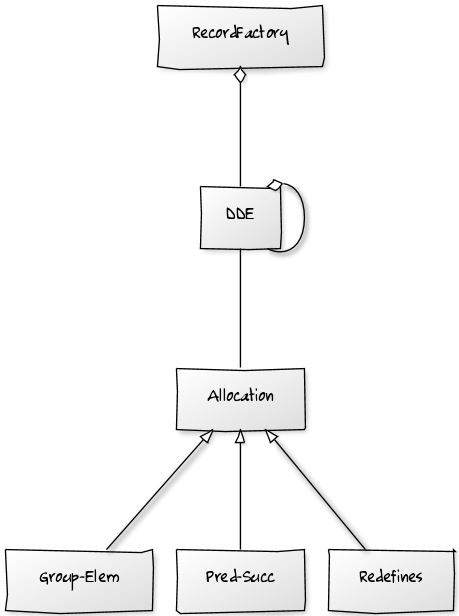
\includegraphics{cobol_redefines.png}
\index{Allocation (class in cobol.defs)}

\begin{fulllineitems}
\phantomsection\label{cobol_defs:cobol.defs.Allocation}\pysigline{\strong{class }\code{cobol.defs.}\bfcode{Allocation}}
The {\hyperref[cobol_defs:cobol.defs.Allocation]{\code{Allocation}}} superclass defines an abstract base
class for the various allocation strategies.

\end{fulllineitems}


\begin{Verbatim}[commandchars=\\\{\}]
\PYG{k}{class} \PYG{n+nc}{Allocation}\PYG{p}{:}
    \PYG{k}{def} \PYG{n+nf}{\PYGZus{}\PYGZus{}init\PYGZus{}\PYGZus{}}\PYG{p}{(} \PYG{n+nb+bp}{self} \PYG{p}{)}\PYG{p}{:}
        \PYG{n+nb+bp}{self}\PYG{o}{.}\PYG{n}{dde}\PYG{o}{=} \PYG{n+nb+bp}{None}
    \PYG{k}{def} \PYG{n+nf}{resolve}\PYG{p}{(} \PYG{n+nb+bp}{self}\PYG{p}{,} \PYG{n}{aDDE} \PYG{p}{)}\PYG{p}{:}
        \PYG{l+s+sd}{\PYGZdq{}\PYGZdq{}\PYGZdq{}Associate back to the owning DDE.\PYGZdq{}\PYGZdq{}\PYGZdq{}}
        \PYG{n+nb+bp}{self}\PYG{o}{.}\PYG{n}{dde}\PYG{o}{=} \PYG{n}{weakref}\PYG{o}{.}\PYG{n}{ref}\PYG{p}{(}\PYG{n}{aDDE}\PYG{p}{)}
\end{Verbatim}
\index{Redefines (class in cobol.defs)}

\begin{fulllineitems}
\phantomsection\label{cobol_defs:cobol.defs.Redefines}\pysigline{\strong{class }\code{cobol.defs.}\bfcode{Redefines}}
The {\hyperref[cobol_defs:cobol.defs.Redefines]{\code{Redefines}}} subclass depends on another element. It uses
the referenced name to look up the offset and total size information.

For this to work, the name must be resolved via the {\hyperref[cobol_defs:cobol.defs.Redefines.resolve]{\code{Redefines.resolve()}}} method.
The {\hyperref[cobol_defs:cobol.defs.resolver]{\code{resolver()}}} function applies the {\hyperref[cobol_defs:cobol.defs.Redefines.resolve]{\code{Redefines.resolve()}}} method throughout the structure.

\end{fulllineitems}


\begin{Verbatim}[commandchars=\\\{\}]
\PYG{k}{class} \PYG{n+nc}{Redefines}\PYG{p}{(}\PYG{n}{Allocation}\PYG{p}{)}\PYG{p}{:}
    \PYG{l+s+sd}{\PYGZdq{}\PYGZdq{}\PYGZdq{}Lookup size and offset from another field we refer to.\PYGZdq{}\PYGZdq{}\PYGZdq{}}
    \PYG{k}{def} \PYG{n+nf}{\PYGZus{}\PYGZus{}init\PYGZus{}\PYGZus{}}\PYG{p}{(} \PYG{n+nb+bp}{self}\PYG{p}{,} \PYG{n}{name}\PYG{p}{,} \PYG{n}{refers\PYGZus{}to}\PYG{o}{=}\PYG{n+nb+bp}{None} \PYG{p}{)}\PYG{p}{:}
        \PYG{n+nb}{super}\PYG{p}{(}\PYG{p}{)}\PYG{o}{.}\PYG{n}{\PYGZus{}\PYGZus{}init\PYGZus{}\PYGZus{}}\PYG{p}{(}\PYG{p}{)}
        \PYG{n+nb+bp}{self}\PYG{o}{.}\PYG{n}{name}\PYG{o}{=} \PYG{n}{name}
        \PYG{n+nb+bp}{self}\PYG{o}{.}\PYG{n}{refers\PYGZus{}to}\PYG{o}{=} \PYG{n}{refers\PYGZus{}to} \PYG{c}{\PYGZsh{} Used for unit testing}
    \PYG{k}{def} \PYG{n+nf}{source}\PYG{p}{(} \PYG{n+nb+bp}{self} \PYG{p}{)}\PYG{p}{:}
        \PYG{k}{return} \PYG{l+s}{\PYGZdq{}}\PYG{l+s}{REDEFINES \PYGZob{}0\PYGZcb{}}\PYG{l+s}{\PYGZdq{}}\PYG{o}{.}\PYG{n}{format}\PYG{p}{(} \PYG{n+nb+bp}{self}\PYG{o}{.}\PYG{n}{refers\PYGZus{}to}\PYG{o}{.}\PYG{n}{name} \PYG{p}{)}
\end{Verbatim}
\index{resolve() (cobol.defs.Redefines method)}

\begin{fulllineitems}
\phantomsection\label{cobol_defs:cobol.defs.Redefines.resolve}\pysiglinewithargsret{\code{Redefines.}\bfcode{resolve}}{\emph{aDDE}}{}
Resolve a DDE name. See our \code{self.refers\_to} to refer to a DDE within
the given structure.

\end{fulllineitems}


\begin{Verbatim}[commandchars=\\\{\}]
\PYG{k}{def} \PYG{n+nf}{resolve}\PYG{p}{(} \PYG{n+nb+bp}{self}\PYG{p}{,} \PYG{n}{aDDE} \PYG{p}{)}\PYG{p}{:}
    \PYG{l+s+sd}{\PYGZdq{}\PYGZdq{}\PYGZdq{}Search the structure for the referenced name.}
\PYG{l+s+sd}{    Must be done before sizing can be done.}
\PYG{l+s+sd}{    \PYGZdq{}\PYGZdq{}\PYGZdq{}}
    \PYG{n+nb}{super}\PYG{p}{(}\PYG{p}{)}\PYG{o}{.}\PYG{n}{resolve}\PYG{p}{(} \PYG{n}{aDDE} \PYG{p}{)}
    \PYG{n+nb+bp}{self}\PYG{o}{.}\PYG{n}{refers\PYGZus{}to}\PYG{o}{=} \PYG{n}{aDDE}\PYG{o}{.}\PYG{n}{top}\PYG{p}{(}\PYG{p}{)}\PYG{o}{.}\PYG{n}{get}\PYG{p}{(} \PYG{n+nb+bp}{self}\PYG{o}{.}\PYG{n}{name} \PYG{p}{)}
\end{Verbatim}
\index{offset() (cobol.defs.Redefines method)}

\begin{fulllineitems}
\phantomsection\label{cobol_defs:cobol.defs.Redefines.offset}\pysiglinewithargsret{\code{Redefines.}\bfcode{offset}}{\emph{offset}}{}
For a redefines, this uses the resolved \code{refers\_to} name and fetches
the offset.

\end{fulllineitems}


\begin{Verbatim}[commandchars=\\\{\}]
\PYG{k}{def} \PYG{n+nf}{offset}\PYG{p}{(} \PYG{n+nb+bp}{self}\PYG{p}{,} \PYG{n}{offset} \PYG{p}{)}\PYG{p}{:}
    \PYG{l+s+sd}{\PYGZdq{}\PYGZdq{}\PYGZdq{}:param offset: computed offset for this relative position.}
\PYG{l+s+sd}{    :return: named DDE element offset instead.}
\PYG{l+s+sd}{    \PYGZdq{}\PYGZdq{}\PYGZdq{}}
    \PYG{k}{return} \PYG{n+nb+bp}{self}\PYG{o}{.}\PYG{n}{refers\PYGZus{}to}\PYG{o}{.}\PYG{n}{offset}
\end{Verbatim}
\index{totalSize() (cobol.defs.Redefines method)}

\begin{fulllineitems}
\phantomsection\label{cobol_defs:cobol.defs.Redefines.totalSize}\pysiglinewithargsret{\code{Redefines.}\bfcode{totalSize}}{}{}
Returns the total size.

\end{fulllineitems}


\begin{Verbatim}[commandchars=\\\{\}]
\PYG{k}{def} \PYG{n+nf}{totalSize}\PYG{p}{(} \PYG{n+nb+bp}{self} \PYG{p}{)}\PYG{p}{:}
    \PYG{l+s+sd}{\PYGZdq{}\PYGZdq{}\PYGZdq{}:return: total size of this DDE include all children and occurs.}
\PYG{l+s+sd}{    \PYGZdq{}\PYGZdq{}\PYGZdq{}}
    \PYG{n}{warnings}\PYG{o}{.}\PYG{n}{warn}\PYG{p}{(}\PYG{l+s}{\PYGZdq{}}\PYG{l+s}{totalSize method is deprecated}\PYG{l+s}{\PYGZdq{}}\PYG{p}{,} \PYG{n+ne}{DeprecationWarning} \PYG{p}{)}
    \PYG{k}{return} \PYG{l+m+mi}{0}
\end{Verbatim}

Note that \code{01} level items may have a REDEFINES.
However, this can never meaningfully redefine anything.
All  \code{01} level definitions start at an offset of 0 by definition.
A copybook may include multiple \code{01} levels with REDEFINES clauses;
an 01-level REDEFINES is irrelevant with respect to offset and size calculations.
\index{Successor (class in cobol.defs)}

\begin{fulllineitems}
\phantomsection\label{cobol_defs:cobol.defs.Successor}\pysigline{\strong{class }\code{cobol.defs.}\bfcode{Successor}}
The {\hyperref[cobol_defs:cobol.defs.Successor]{\code{Successor}}}
subclass does not depend on a named element, it depends on the immediate
predecessor. It uses that contextual offset and size information provided by
the {\hyperref[cobol_defs:cobol.defs.setSizeAndOffset]{\code{setSizeAndOffset()}}} function.

\end{fulllineitems}


\begin{Verbatim}[commandchars=\\\{\}]
\PYG{k}{class} \PYG{n+nc}{Successor}\PYG{p}{(}\PYG{n}{Allocation}\PYG{p}{)}\PYG{p}{:}
    \PYG{l+s+sd}{\PYGZdq{}\PYGZdq{}\PYGZdq{}More typical case is that the DDE follows it\PYGZsq{}s predecessor.}
\PYG{l+s+sd}{    It\PYGZsq{}s not first in a group, nor is it a redefines.}
\PYG{l+s+sd}{    \PYGZdq{}\PYGZdq{}\PYGZdq{}}
    \PYG{k}{def} \PYG{n+nf}{\PYGZus{}\PYGZus{}init\PYGZus{}\PYGZus{}}\PYG{p}{(} \PYG{n+nb+bp}{self}\PYG{p}{,} \PYG{n}{pred} \PYG{p}{)}\PYG{p}{:}
        \PYG{n+nb}{super}\PYG{p}{(}\PYG{p}{)}\PYG{o}{.}\PYG{n}{\PYGZus{}\PYGZus{}init\PYGZus{}\PYGZus{}}\PYG{p}{(}\PYG{p}{)}
        \PYG{n+nb+bp}{self}\PYG{o}{.}\PYG{n}{refers\PYGZus{}to}\PYG{o}{=} \PYG{n}{pred}
    \PYG{k}{def} \PYG{n+nf}{source}\PYG{p}{(} \PYG{n+nb+bp}{self} \PYG{p}{)}\PYG{p}{:}
        \PYG{k}{return} \PYG{l+s}{\PYGZdq{}}\PYG{l+s}{\PYGZdq{}}
\end{Verbatim}
\index{offset() (cobol.defs.Successor method)}

\begin{fulllineitems}
\phantomsection\label{cobol_defs:cobol.defs.Successor.offset}\pysiglinewithargsret{\code{Successor.}\bfcode{offset}}{\emph{offset}}{}
For a successor, we use the predecessor in the \code{refers\_to} field
to track down the offset of the predecessor.

This field's offset is predecessor offset + predecessor total size.

The predecessor may have to do some thinking to get its total size or
offset because of an Occurs Depending On situation.

\end{fulllineitems}


\begin{Verbatim}[commandchars=\\\{\}]
\PYG{k}{def} \PYG{n+nf}{offset}\PYG{p}{(} \PYG{n+nb+bp}{self}\PYG{p}{,} \PYG{n}{offset} \PYG{p}{)}\PYG{p}{:}
    \PYG{l+s+sd}{\PYGZdq{}\PYGZdq{}\PYGZdq{}:param offset: computed offset to this point.}
\PYG{l+s+sd}{    :return: computed offset}
\PYG{l+s+sd}{    \PYGZdq{}\PYGZdq{}\PYGZdq{}}
    \PYG{k}{return} \PYG{n}{offset}
\end{Verbatim}
\index{totalSize() (cobol.defs.Successor method)}

\begin{fulllineitems}
\phantomsection\label{cobol_defs:cobol.defs.Successor.totalSize}\pysiglinewithargsret{\code{Successor.}\bfcode{totalSize}}{}{}
The total size of a field with occurs depending on requires a record with live data.
Otherwise, the total size is trivially computed from the DDE definition.

\end{fulllineitems}


\begin{Verbatim}[commandchars=\\\{\}]
\PYG{k}{def} \PYG{n+nf}{totalSize}\PYG{p}{(} \PYG{n+nb+bp}{self} \PYG{p}{)}\PYG{p}{:}
    \PYG{l+s+sd}{\PYGZdq{}\PYGZdq{}\PYGZdq{}:return: total size of this DDE include all children and occurs.}
\PYG{l+s+sd}{    \PYGZdq{}\PYGZdq{}\PYGZdq{}}
    \PYG{n}{warnings}\PYG{o}{.}\PYG{n}{warn}\PYG{p}{(}\PYG{l+s}{\PYGZdq{}}\PYG{l+s}{totalSize method is deprecated}\PYG{l+s}{\PYGZdq{}}\PYG{p}{,} \PYG{n+ne}{DeprecationWarning} \PYG{p}{)}
    \PYG{k}{return} \PYG{n+nb+bp}{self}\PYG{o}{.}\PYG{n}{dde}\PYG{p}{(}\PYG{p}{)}\PYG{o}{.}\PYG{n}{totalSize}
\end{Verbatim}
\index{Group (class in cobol.defs)}

\begin{fulllineitems}
\phantomsection\label{cobol_defs:cobol.defs.Group}\pysigline{\strong{class }\code{cobol.defs.}\bfcode{Group}}
This subclass does not depend on a named element, it depends on the immediate
parent group. It uses that contextual offset and size information provided by
the {\hyperref[cobol_defs:cobol.defs.setSizeAndOffset]{\code{setSizeAndOffset()}}} function.

\end{fulllineitems}


\begin{Verbatim}[commandchars=\\\{\}]
\PYG{k}{class} \PYG{n+nc}{Group}\PYG{p}{(}\PYG{n}{Allocation}\PYG{p}{)}\PYG{p}{:}
    \PYG{l+s+sd}{\PYGZdq{}\PYGZdq{}\PYGZdq{}More typical case is that the DDE is first under a parent.\PYGZdq{}\PYGZdq{}\PYGZdq{}}
    \PYG{k}{def} \PYG{n+nf}{\PYGZus{}\PYGZus{}init\PYGZus{}\PYGZus{}}\PYG{p}{(} \PYG{n+nb+bp}{self} \PYG{p}{)}\PYG{p}{:}
        \PYG{n+nb}{super}\PYG{p}{(}\PYG{p}{)}\PYG{o}{.}\PYG{n}{\PYGZus{}\PYGZus{}init\PYGZus{}\PYGZus{}}\PYG{p}{(}\PYG{p}{)}

    \PYG{k}{def} \PYG{n+nf}{source}\PYG{p}{(} \PYG{n+nb+bp}{self} \PYG{p}{)}\PYG{p}{:}
        \PYG{k}{return} \PYG{l+s}{\PYGZdq{}}\PYG{l+s}{\PYGZdq{}}
\end{Verbatim}
\index{offset() (cobol.defs.Group method)}

\begin{fulllineitems}
\phantomsection\label{cobol_defs:cobol.defs.Group.offset}\pysiglinewithargsret{\code{Group.}\bfcode{offset}}{\emph{offset}}{}
For the first item in a group, we use the group parent in the \code{dde} field
to track down the offset of the group we're a member of.

This field's offset is the group offset, since this field is first in the group.

The group may have to do some recursive processing to get its predecessor's total size or
offset because of an Occurs Depending On situation.

\end{fulllineitems}


\begin{Verbatim}[commandchars=\\\{\}]
\PYG{k}{def} \PYG{n+nf}{offset}\PYG{p}{(} \PYG{n+nb+bp}{self}\PYG{p}{,} \PYG{n}{offset} \PYG{p}{)}\PYG{p}{:}
    \PYG{l+s+sd}{\PYGZdq{}\PYGZdq{}\PYGZdq{}:param offset: computed offset}
\PYG{l+s+sd}{    :return: computed offset}
\PYG{l+s+sd}{    \PYGZdq{}\PYGZdq{}\PYGZdq{}}
    \PYG{k}{return} \PYG{n}{offset}
\end{Verbatim}
\index{totalSize() (cobol.defs.Group method)}

\begin{fulllineitems}
\phantomsection\label{cobol_defs:cobol.defs.Group.totalSize}\pysiglinewithargsret{\code{Group.}\bfcode{totalSize}}{}{}
This is essentially the same as the successor -- it's merely an item within a DDE,
we just track the first items separately with this subclass so that they
can refer to the parent to walk up the tree.

\end{fulllineitems}


\begin{Verbatim}[commandchars=\\\{\}]
\PYG{k}{def} \PYG{n+nf}{totalSize}\PYG{p}{(} \PYG{n+nb+bp}{self} \PYG{p}{)}\PYG{p}{:}
    \PYG{l+s+sd}{\PYGZdq{}\PYGZdq{}\PYGZdq{}:return: total size of this DDE include all children and occurs.}
\PYG{l+s+sd}{    \PYGZdq{}\PYGZdq{}\PYGZdq{}}
    \PYG{n}{warnings}\PYG{o}{.}\PYG{n}{warn}\PYG{p}{(}\PYG{l+s}{\PYGZdq{}}\PYG{l+s}{totalSize method is deprecated}\PYG{l+s}{\PYGZdq{}}\PYG{p}{,} \PYG{n+ne}{DeprecationWarning} \PYG{p}{)}
    \PYG{k}{return} \PYG{n+nb+bp}{self}\PYG{o}{.}\PYG{n}{dde}\PYG{p}{(}\PYG{p}{)}\PYG{o}{.}\PYG{n}{totalSize}
\end{Verbatim}


\subparagraph{Occurs Strategy Hierarchy}
\label{cobol_defs:occurs-strategy-hierarchy}
There are three species of Occurs clauses.
\begin{itemize}
\item {} 
Format 1. Fixed OCCURS with a number.

\item {} 
Format 2. Variable OCCURS DEPENDING ON with a number and a name.
The {\hyperref[cobol_defs:cobol.defs.resolver]{\code{resolver()}}} function sorts out the reference.
Similar to the way REDEFINES is handled.

\item {} 
Format 0. No Occurs, effectively OCCURS == 1 with no dimensionality issues.

\end{itemize}

This means that the \code{number} attribute must be derived EITHER from the definition
or a data record. For ODO, we need to bind the definition to a record.

\begin{notice}{warning}{Warning:}
Dependencies between DDE and Attribute

An OCCURS is a feature of the DDE.
Data access, however, requires the {\hyperref[schema:schema.Attribute]{\code{schema.Attribute}}}.
There's no \textbf{direct} linkage from {\hyperref[cobol_defs:cobol.defs.DDE]{\code{cobol.defs.DDE}}} to {\hyperref[schema:schema.Attribute]{\code{schema.Attribute}}}.
There is linkage from {\hyperref[schema:schema.Attribute]{\code{schema.Attribute}}} to {\hyperref[cobol_defs:cobol.defs.DDE]{\code{cobol.defs.DDE}}}.

It seems best to have Attribute independent of any particular
source. A schema may not necessarily come from COBOL.

However.

To facilitate a DDE-oriented dump of raw data or specific fields of a COBOL
file, we include a \code{weakref} from the \code{DDE} to the \code{Attribute} created
from that DDE.
\end{notice}

The overall top-most parent DDE associated with this object is \code{self.dde().top()}.
\index{Occurs (class in cobol.defs)}

\begin{fulllineitems}
\phantomsection\label{cobol_defs:cobol.defs.Occurs}\pysigline{\strong{class }\code{cobol.defs.}\bfcode{Occurs}}
Abstract superclass for an Occurs clause.

\end{fulllineitems}


\begin{Verbatim}[commandchars=\\\{\}]
\PYG{k}{class} \PYG{n+nc}{Occurs}\PYG{p}{:}
    \PYG{l+s+sd}{\PYGZdq{}\PYGZdq{}\PYGZdq{}No OCCURS clause present. Data from a row is irrelevant.\PYGZdq{}\PYGZdq{}\PYGZdq{}}
    \PYG{n}{default}\PYG{o}{=} \PYG{n+nb+bp}{True}
    \PYG{n}{static}\PYG{o}{=} \PYG{n+nb+bp}{True}
    \PYG{k}{def} \PYG{n+nf}{\PYGZus{}\PYGZus{}str\PYGZus{}\PYGZus{}}\PYG{p}{(} \PYG{n+nb+bp}{self} \PYG{p}{)}\PYG{p}{:}
        \PYG{k}{return} \PYG{l+s}{\PYGZdq{}}\PYG{l+s}{\PYGZdq{}}
    \PYG{k}{def} \PYG{n+nf}{resolve}\PYG{p}{(} \PYG{n+nb+bp}{self}\PYG{p}{,} \PYG{n}{aDDE} \PYG{p}{)}\PYG{p}{:}
        \PYG{n+nb+bp}{self}\PYG{o}{.}\PYG{n}{dde}\PYG{o}{=} \PYG{n}{weakref}\PYG{o}{.}\PYG{n}{ref}\PYG{p}{(}\PYG{n}{aDDE}\PYG{p}{)}
    \PYG{k}{def} \PYG{n+nf}{number}\PYG{p}{(} \PYG{n+nb+bp}{self}\PYG{p}{,} \PYG{n}{aRow} \PYG{p}{)}\PYG{p}{:}
        \PYG{k}{return} \PYG{l+m+mi}{1}
\end{Verbatim}
\index{OccursFixed (class in cobol.defs)}

\begin{fulllineitems}
\phantomsection\label{cobol_defs:cobol.defs.OccursFixed}\pysigline{\strong{class }\code{cobol.defs.}\bfcode{OccursFixed}}
Occurs clause with a simple fixed number of occurrences.

\end{fulllineitems}


\begin{Verbatim}[commandchars=\\\{\}]
\PYG{k}{class} \PYG{n+nc}{OccursFixed}\PYG{p}{(} \PYG{n}{Occurs} \PYG{p}{)}\PYG{p}{:}
    \PYG{l+s+sd}{\PYGZdq{}\PYGZdq{}\PYGZdq{}OCCURS n TIMES. Data from a row is irrelevant.\PYGZdq{}\PYGZdq{}\PYGZdq{}}
    \PYG{n}{default}\PYG{o}{=} \PYG{n+nb+bp}{False}
    \PYG{n}{static}\PYG{o}{=} \PYG{n+nb+bp}{True}
    \PYG{k}{def} \PYG{n+nf}{\PYGZus{}\PYGZus{}init\PYGZus{}\PYGZus{}}\PYG{p}{(} \PYG{n+nb+bp}{self}\PYG{p}{,} \PYG{n}{number} \PYG{p}{)}\PYG{p}{:}
        \PYG{n+nb+bp}{self}\PYG{o}{.}\PYG{n}{\PYGZus{}number}\PYG{o}{=} \PYG{n+nb}{int}\PYG{p}{(}\PYG{n}{number}\PYG{p}{)}
    \PYG{k}{def} \PYG{n+nf}{\PYGZus{}\PYGZus{}str\PYGZus{}\PYGZus{}}\PYG{p}{(} \PYG{n+nb+bp}{self} \PYG{p}{)}\PYG{p}{:}
        \PYG{k}{return} \PYG{l+s}{\PYGZdq{}}\PYG{l+s}{OCCURS \PYGZob{}0\PYGZcb{}}\PYG{l+s}{\PYGZdq{}}\PYG{o}{.}\PYG{n}{format}\PYG{p}{(}\PYG{n+nb+bp}{self}\PYG{o}{.}\PYG{n}{number}\PYG{p}{)}
    \PYG{k}{def} \PYG{n+nf}{resolve}\PYG{p}{(} \PYG{n+nb+bp}{self}\PYG{p}{,} \PYG{n}{aDDE} \PYG{p}{)}\PYG{p}{:}
        \PYG{n+nb}{super}\PYG{p}{(}\PYG{p}{)}\PYG{o}{.}\PYG{n}{resolve}\PYG{p}{(}\PYG{n}{aDDE}\PYG{p}{)}
    \PYG{k}{def} \PYG{n+nf}{number}\PYG{p}{(} \PYG{n+nb+bp}{self}\PYG{p}{,} \PYG{n}{aRow} \PYG{p}{)}\PYG{p}{:}
        \PYG{k}{return} \PYG{n+nb+bp}{self}\PYG{o}{.}\PYG{n}{\PYGZus{}number}
\end{Verbatim}
\index{OccursDependingOn (class in cobol.defs)}

\begin{fulllineitems}
\phantomsection\label{cobol_defs:cobol.defs.OccursDependingOn}\pysigline{\strong{class }\code{cobol.defs.}\bfcode{OccursDependingOn}}
Occurs clause with a DEPENDING ON option.

\end{fulllineitems}


\begin{Verbatim}[commandchars=\\\{\}]
\PYG{k}{class} \PYG{n+nc}{OccursDependingOn}\PYG{p}{(} \PYG{n}{Occurs} \PYG{p}{)}\PYG{p}{:}
    \PYG{l+s+sd}{\PYGZdq{}\PYGZdq{}\PYGZdq{}OCCURS TO n TIMES DEPENDING ON name. Data from a row is required.\PYGZdq{}\PYGZdq{}\PYGZdq{}}
    \PYG{n}{default}\PYG{o}{=} \PYG{n+nb+bp}{False}
    \PYG{n}{static}\PYG{o}{=} \PYG{n+nb+bp}{False}
    \PYG{k}{def} \PYG{n+nf}{\PYGZus{}\PYGZus{}init\PYGZus{}\PYGZus{}}\PYG{p}{(} \PYG{n+nb+bp}{self}\PYG{p}{,} \PYG{n}{name}\PYG{p}{,} \PYG{n}{limit} \PYG{p}{)}\PYG{p}{:}
        \PYG{n+nb+bp}{self}\PYG{o}{.}\PYG{n}{name}\PYG{o}{=} \PYG{n}{name}
        \PYG{n+nb+bp}{self}\PYG{o}{.}\PYG{n}{limit}\PYG{o}{=} \PYG{n}{limit}
        \PYG{n+nb+bp}{self}\PYG{o}{.}\PYG{n}{refers\PYGZus{}to}\PYG{o}{=} \PYG{n+nb+bp}{None}
        \PYG{n+nb+bp}{self}\PYG{o}{.}\PYG{n}{attr}\PYG{o}{=} \PYG{n+nb+bp}{None}
    \PYG{k}{def} \PYG{n+nf}{\PYGZus{}\PYGZus{}str\PYGZus{}\PYGZus{}}\PYG{p}{(} \PYG{n+nb+bp}{self} \PYG{p}{)}\PYG{p}{:}
        \PYG{k}{return} \PYG{l+s}{\PYGZdq{}}\PYG{l+s}{OCCURS TO \PYGZob{}0\PYGZcb{} DEPENDING ON \PYGZob{}1\PYGZcb{}}\PYG{l+s}{\PYGZdq{}}\PYG{o}{.}\PYG{n}{format}\PYG{p}{(}\PYG{n+nb+bp}{self}\PYG{o}{.}\PYG{n}{limit}\PYG{p}{,} \PYG{n+nb+bp}{self}\PYG{o}{.}\PYG{n}{name}\PYG{p}{)}
    \PYG{k}{def} \PYG{n+nf}{resolve}\PYG{p}{(} \PYG{n+nb+bp}{self}\PYG{p}{,} \PYG{n}{aDDE} \PYG{p}{)}\PYG{p}{:}
        \PYG{n+nb}{super}\PYG{p}{(}\PYG{p}{)}\PYG{o}{.}\PYG{n}{resolve}\PYG{p}{(}\PYG{n}{aDDE}\PYG{p}{)}
        \PYG{n+nb+bp}{self}\PYG{o}{.}\PYG{n}{refers\PYGZus{}to}\PYG{o}{=} \PYG{n}{aDDE}\PYG{o}{.}\PYG{n}{top}\PYG{p}{(}\PYG{p}{)}\PYG{o}{.}\PYG{n}{get}\PYG{p}{(} \PYG{n+nb+bp}{self}\PYG{o}{.}\PYG{n}{name} \PYG{p}{)}
    \PYG{k}{def} \PYG{n+nf}{number}\PYG{p}{(} \PYG{n+nb+bp}{self}\PYG{p}{,} \PYG{n}{aRow} \PYG{p}{)}\PYG{p}{:}
        \PYG{l+s+sd}{\PYGZdq{}\PYGZdq{}\PYGZdq{}aRow.cell( schema.get(self.name) ) should have a numeric value.\PYGZdq{}\PYGZdq{}\PYGZdq{}}
        \PYG{k}{if} \PYG{n+nb+bp}{self}\PYG{o}{.}\PYG{n}{attr} \PYG{o+ow}{is} \PYG{n+nb+bp}{None}\PYG{p}{:}
            \PYG{n}{schema\PYGZus{}dict}\PYG{o}{=} \PYG{n+nb}{dict}\PYG{p}{(} \PYG{p}{(}\PYG{n}{a}\PYG{o}{.}\PYG{n}{name}\PYG{p}{,} \PYG{n}{a}\PYG{p}{)} \PYG{k}{for} \PYG{n}{a} \PYG{o+ow}{in} \PYG{n}{aRow}\PYG{o}{.}\PYG{n}{sheet}\PYG{o}{.}\PYG{n}{schema} \PYG{p}{)}
            \PYG{n+nb+bp}{self}\PYG{o}{.}\PYG{n}{attr}\PYG{o}{=} \PYG{n}{schema\PYGZus{}dict}\PYG{p}{[}\PYG{n+nb+bp}{self}\PYG{o}{.}\PYG{n}{name}\PYG{p}{]}
        \PYG{c}{\PYGZsh{}\PYGZsh{} logger.debug( \PYGZdq{}Getting \PYGZob{}0\PYGZcb{} from \PYGZob{}1\PYGZcb{}\PYGZdq{}.format(self.attr,aRow) )}
        \PYG{n}{value}\PYG{o}{=} \PYG{n}{aRow}\PYG{o}{.}\PYG{n}{cell}\PYG{p}{(} \PYG{n+nb+bp}{self}\PYG{o}{.}\PYG{n}{attr} \PYG{p}{)}\PYG{o}{.}\PYG{n}{to\PYGZus{}int}\PYG{p}{(}\PYG{p}{)}
        \PYG{k}{return} \PYG{n}{value}
\end{Verbatim}
\index{OccursDependingOnLimit (class in cobol.defs)}

\begin{fulllineitems}
\phantomsection\label{cobol_defs:cobol.defs.OccursDependingOnLimit}\pysigline{\strong{class }\code{cobol.defs.}\bfcode{OccursDependingOnLimit}}
This is an extension to OccursDependingOn. It limits the ODO clause to the defined
upper bound.

If we have \code{05 SOMETHING OCCURS 1 TO 5 TIMES DEPENDING ON X} and
the value of \code{X} is greater than 5, the maximum defined value, 5, is used.

This entirely hypothetical as a possible fix to a problem. It's probably a
Very Bad Idea, and should be removed.

See \href{http://pic.dhe.ibm.com/infocenter/ratdevz/v8r0/index.jsp?topic=\%2Fcom.ibm.ent.cbl.zos.doc\%2Ftopics\%2FMG\%2Figymch1027.htm}{http://pic.dhe.ibm.com/infocenter/ratdevz/v8r0/index.jsp?topic=\%2Fcom.ibm.ent.cbl.zos.doc\%2Ftopics\%2FMG\%2Figymch1027.htm}
\begin{quote}

``When the maximum length is used, it is not necessary to initialize the ODO object before the table receives data.''

``When TABLE-GROUP-1 is a receiving item, Enterprise COBOL moves the maximum number of character positions for it (450 bytes for TABLE-1 plus two bytes for ODO-KEY-1). Therefore, you need not initialize the length of TABLE-1 before moving the SEND-ITEM-1 data into the table.''
\end{quote}

Based on this (and bad data seen in the wild) we deduce that this upper limit
clamping \textbf{may} be a language  feature.

\end{fulllineitems}


\begin{Verbatim}[commandchars=\\\{\}]
\PYG{k}{class} \PYG{n+nc}{OccursDependingOnLimit}\PYG{p}{(} \PYG{n}{OccursDependingOn} \PYG{p}{)}\PYG{p}{:}
    \PYG{l+s+sd}{\PYGZdq{}\PYGZdq{}\PYGZdq{}OCCURS TO n TIMES DEPENDING ON name. Data is required.}
\PYG{l+s+sd}{    This will clamp the result at the given upper limit.}
\PYG{l+s+sd}{    \PYGZdq{}\PYGZdq{}\PYGZdq{}}
    \PYG{k}{def} \PYG{n+nf}{number}\PYG{p}{(} \PYG{n+nb+bp}{self}\PYG{p}{,} \PYG{n}{aRow} \PYG{p}{)}\PYG{p}{:}
        \PYG{n}{value}\PYG{o}{=} \PYG{n+nb}{super}\PYG{p}{(}\PYG{p}{)}\PYG{o}{.}\PYG{n}{number}\PYG{p}{(} \PYG{n}{aRow} \PYG{p}{)}
        \PYG{k}{if} \PYG{n}{value} \PYG{o}{\PYGZgt{}} \PYG{n+nb+bp}{self}\PYG{o}{.}\PYG{n}{limit}\PYG{p}{:}
            \PYG{k}{return} \PYG{n+nb+bp}{self}\PYG{o}{.}\PYG{n}{limit}
        \PYG{k}{return} \PYG{n}{value}
\end{Verbatim}


\subparagraph{DDE Class}
\label{cobol_defs:dde-class}\index{DDE (class in cobol.defs)}

\begin{fulllineitems}
\phantomsection\label{cobol_defs:cobol.defs.DDE}\pysigline{\strong{class }\code{cobol.defs.}\bfcode{DDE}}
The {\hyperref[cobol_defs:cobol.defs.DDE]{\code{DDE}}} class itself defines a single element (group or elementary) of a
record.  There are several broad areas of functionality for a DDE:
(1) construction, (2) reporting and decoration, (3) processing record data.

The class definition includes the attributes determined at
parse time, attributes added during decoration time and
attributes used during decoration processing.

As noted above, Group-level vs. Elementary-level \emph{could} be separate subclasses of DDE.
They aren't right now, since group-level items can be used in an application program
like elementary items.

A group-level item contains subsidiary DDE's and has no PICTURE clause.
An elementary-level DDE is defined by having a PICTURE clause.

All group-level DDE's are effectively string-type data.
An elementary-level DDE with a numeric PICTURE is numeric-type data.  It can
be usage display or usage computational.  An elementary-level DDE with a string PICTURE is string-type data.

Occurs and Redefines can occur at any level.

Each entry is defined by the following attributes:
\index{level (cobol.defs.DDE attribute)}

\begin{fulllineitems}
\phantomsection\label{cobol_defs:cobol.defs.DDE.level}\pysigline{\bfcode{level}}
COBOL level number 01 to 49, 66 or 88.

\end{fulllineitems}

\index{myName (cobol.defs.DDE attribute)}

\begin{fulllineitems}
\phantomsection\label{cobol_defs:cobol.defs.DDE.myName}\pysigline{\bfcode{myName}}
COBOL variable name

\end{fulllineitems}

\index{occurs (cobol.defs.DDE attribute)}

\begin{fulllineitems}
\phantomsection\label{cobol_defs:cobol.defs.DDE.occurs}\pysigline{\bfcode{occurs}}
An instance of {\hyperref[cobol_defs:cobol.defs.Occurs]{\code{Occurs}}}.
the number of occurrences. The default is 1, which we call ``format 0''.
There are two defined formats: format 1 has a fixed number of occurrences;
format 2 is the Occurs Depending On with a variable number of occurrences.

\end{fulllineitems}

\index{picture (cobol.defs.DDE attribute)}

\begin{fulllineitems}
\phantomsection\label{cobol_defs:cobol.defs.DDE.picture}\pysigline{\bfcode{picture}}
the exploded picture clause, with ()'s expanded

\end{fulllineitems}

\index{initValue (cobol.defs.DDE attribute)}

\begin{fulllineitems}
\phantomsection\label{cobol_defs:cobol.defs.DDE.initValue}\pysigline{\bfcode{initValue}}
any initial value provided

\end{fulllineitems}

\index{allocation (cobol.defs.DDE attribute)}

\begin{fulllineitems}
\phantomsection\label{cobol_defs:cobol.defs.DDE.allocation}\pysigline{\bfcode{allocation}}
an instance of {\hyperref[cobol_defs:cobol.defs.Allocation]{\code{Allocation}}} used to compute the offset and total size.

\end{fulllineitems}

\index{usage (cobol.defs.DDE attribute)}

\begin{fulllineitems}
\phantomsection\label{cobol_defs:cobol.defs.DDE.usage}\pysigline{\bfcode{usage}}
an instance of {\hyperref[cobol_defs:cobol.defs.Usage]{\code{Usage}}} to delegate data conversion properly.
The actual conversion is handled by the workbook.

\end{fulllineitems}

\index{contains (cobol.defs.DDE attribute)}

\begin{fulllineitems}
\phantomsection\label{cobol_defs:cobol.defs.DDE.contains}\pysigline{\bfcode{contains}}
the list of contained fields within a group

\end{fulllineitems}

\index{parent (cobol.defs.DDE attribute)}

\begin{fulllineitems}
\phantomsection\label{cobol_defs:cobol.defs.DDE.parent}\pysigline{\bfcode{parent}}
A weakref to the immediate parent DDE

\end{fulllineitems}

\index{top (cobol.defs.DDE attribute)}

\begin{fulllineitems}
\phantomsection\label{cobol_defs:cobol.defs.DDE.top}\pysigline{\bfcode{top}}
A weakref to the overall record definition DDE.

\end{fulllineitems}


The following decorations are applied by functions that traverse the DDE structure.
\index{sizeScalePrecision (cobol.defs.DDE attribute)}

\begin{fulllineitems}
\phantomsection\label{cobol_defs:cobol.defs.DDE.sizeScalePrecision}\pysigline{\bfcode{sizeScalePrecision}}
\code{Picture} namedtuple with details derived from parsing the PICTURE clause

\end{fulllineitems}

\index{size (cobol.defs.DDE attribute)}

\begin{fulllineitems}
\phantomsection\label{cobol_defs:cobol.defs.DDE.size}\pysigline{\bfcode{size}}
the size of an individual occurrence

\end{fulllineitems}


The following features may have to be computed lazily if there's an Occurs
Depending On. Otherwise they can be computed eagerly.
\index{variably\_located (cobol.defs.DDE attribute)}

\begin{fulllineitems}
\phantomsection\label{cobol_defs:cobol.defs.DDE.variably_located}\pysigline{\bfcode{variably\_located}}
Variably Located if any this element or any child has Occurs Depending On.
Otherwise (no ODO) the DDE is Statically Located.
Actually, only element \textbf{after} the ODO element are variably located. But it's simpler
to treat the whole record as variable.

\end{fulllineitems}

\index{offset (cobol.defs.DDE attribute)}

\begin{fulllineitems}
\phantomsection\label{cobol_defs:cobol.defs.DDE.offset}\pysigline{\bfcode{offset}}
offset to this field from start of record.

\end{fulllineitems}

\index{totalSize (cobol.defs.DDE attribute)}

\begin{fulllineitems}
\phantomsection\label{cobol_defs:cobol.defs.DDE.totalSize}\pysigline{\bfcode{totalSize}}
overall size of this item, including all occurrences.

\end{fulllineitems}


Additionally, this item -- in a way -- breaks the dependencies between
a {\hyperref[schema:schema.Attribute]{\code{schema.Attribute}}} and a DDE. It's appropriate for an Attribute
to depend on a DDE, but the reverse isn't proper. However, we DDE
referring to an attribute anyway.
\index{attribute (cobol.defs.DDE attribute)}

\begin{fulllineitems}
\phantomsection\label{cobol_defs:cobol.defs.DDE.attribute}\pysigline{\bfcode{attribute}}
weakref to the {\hyperref[schema:schema.Attribute]{\code{schema.Attribute}}} built from this DDE.

\end{fulllineitems}


\end{fulllineitems}


\begin{Verbatim}[commandchars=\\\{\}]
\PYG{k}{class} \PYG{n+nc}{DDE}\PYG{p}{:}
    \PYG{l+s+sd}{\PYGZdq{}\PYGZdq{}\PYGZdq{}A Data Description Entry.}
\PYG{l+s+sd}{    \PYGZdq{}\PYGZdq{}\PYGZdq{}}
    \PYG{k}{def} \PYG{n+nf}{\PYGZus{}\PYGZus{}init\PYGZus{}\PYGZus{}}\PYG{p}{(} \PYG{n+nb+bp}{self}\PYG{p}{,} \PYG{n}{level}\PYG{p}{,} \PYG{n}{name}\PYG{p}{,} \PYG{n}{usage}\PYG{o}{=}\PYG{n+nb+bp}{None}\PYG{p}{,} \PYG{n}{occurs}\PYG{o}{=}\PYG{n+nb+bp}{None}\PYG{p}{,} \PYG{n}{redefines}\PYG{o}{=}\PYG{n+nb+bp}{None}\PYG{p}{,}
        \PYG{n}{initValue}\PYG{o}{=}\PYG{n+nb+bp}{None}\PYG{p}{,} \PYG{n}{pic}\PYG{o}{=}\PYG{n+nb+bp}{None}\PYG{p}{,} \PYG{n}{sizeScalePrecision}\PYG{o}{=}\PYG{n+nb+bp}{None} \PYG{p}{)}\PYG{p}{:}
        \PYG{l+s+sd}{\PYGZdq{}\PYGZdq{}\PYGZdq{}Build this with the results of parsing the various clauses.}
\PYG{l+s+sd}{        \PYGZdq{}\PYGZdq{}\PYGZdq{}}
        \PYG{n+nb+bp}{self}\PYG{o}{.}\PYG{n}{level}\PYG{o}{=} \PYG{n}{level}
        \PYG{n+nb+bp}{self}\PYG{o}{.}\PYG{n}{name}\PYG{o}{=} \PYG{n}{name}
        \PYG{n+nb+bp}{self}\PYG{o}{.}\PYG{n}{occurs}\PYG{o}{=} \PYG{n}{occurs} \PYG{k}{if} \PYG{n}{occurs} \PYG{o+ow}{is} \PYG{o+ow}{not} \PYG{n+nb+bp}{None} \PYG{k}{else} \PYG{n}{Occurs}\PYG{p}{(}\PYG{p}{)}
        \PYG{n+nb+bp}{self}\PYG{o}{.}\PYG{n}{picture}\PYG{o}{=} \PYG{n}{pic} \PYG{c}{\PYGZsh{} source, prior to parsing, below.}
        \PYG{n+nb+bp}{self}\PYG{o}{.}\PYG{n}{allocation}\PYG{o}{=} \PYG{n}{redefines} \PYG{c}{\PYGZsh{} Redefines or Successor or Group}
        \PYG{n+nb+bp}{self}\PYG{o}{.}\PYG{n}{usage}\PYG{o}{=} \PYG{n}{usage}
        \PYG{n+nb+bp}{self}\PYG{o}{.}\PYG{n}{initValue}\PYG{o}{=} \PYG{n}{initValue}

        \PYG{c}{\PYGZsh{} Parsed picture information}
        \PYG{n+nb+bp}{self}\PYG{o}{.}\PYG{n}{sizeScalePrecision}\PYG{o}{=} \PYG{n}{sizeScalePrecision}

        \PYG{c}{\PYGZsh{} Relationships}
        \PYG{n+nb+bp}{self}\PYG{o}{.}\PYG{n}{indent}\PYG{o}{=} \PYG{l+m+mi}{0}
        \PYG{n+nb+bp}{self}\PYG{o}{.}\PYG{n}{children}\PYG{o}{=} \PYG{p}{[}\PYG{p}{]}
        \PYG{n+nb+bp}{self}\PYG{o}{.}\PYG{n}{top}\PYG{o}{=} \PYG{n+nb+bp}{None} \PYG{c}{\PYGZsh{} must be a weakref.ref()}
        \PYG{n+nb+bp}{self}\PYG{o}{.}\PYG{n}{parent}\PYG{o}{=} \PYG{n+nb+bp}{None} \PYG{c}{\PYGZsh{} must be a weakref.ref()}

        \PYG{c}{\PYGZsh{} Derived property from the picture clause}
        \PYG{n+nb+bp}{self}\PYG{o}{.}\PYG{n}{size}\PYG{o}{=} \PYG{n+nb+bp}{self}\PYG{o}{.}\PYG{n}{usage}\PYG{o}{.}\PYG{n}{size}\PYG{p}{(}\PYG{p}{)}

        \PYG{c}{\PYGZsh{} Because of ODO, these cannot always be computed statically.}
        \PYG{n+nb+bp}{self}\PYG{o}{.}\PYG{n}{offset}\PYG{o}{=} \PYG{l+m+mi}{0} \PYG{c}{\PYGZsh{} self.allocation.refers\PYGZus{}to.offset + self.allocation.refers\PYGZus{}to.total\PYGZus{}size}
        \PYG{n+nb+bp}{self}\PYG{o}{.}\PYG{n}{totalSize}\PYG{o}{=} \PYG{l+m+mi}{0} \PYG{c}{\PYGZsh{} self.size * self.occurs.number(aRow)}

        \PYG{c}{\PYGZsh{} Derived attribute created from this DDE.}
        \PYG{n+nb+bp}{self}\PYG{o}{.}\PYG{n}{attribute}\PYG{o}{=} \PYG{n+nb+bp}{None}

    \PYG{k}{def} \PYG{n+nf}{\PYGZus{}\PYGZus{}repr\PYGZus{}\PYGZus{}}\PYG{p}{(} \PYG{n+nb+bp}{self} \PYG{p}{)}\PYG{p}{:}
        \PYG{k}{return} \PYG{l+s}{\PYGZdq{}}\PYG{l+s}{\PYGZob{}:s\PYGZcb{} \PYGZob{}:s\PYGZcb{} \PYGZob{}:s\PYGZcb{}}\PYG{l+s}{\PYGZdq{}}\PYG{o}{.}\PYG{n}{format}\PYG{p}{(} \PYG{n+nb+bp}{self}\PYG{o}{.}\PYG{n}{level}\PYG{p}{,} \PYG{n+nb+bp}{self}\PYG{o}{.}\PYG{n}{name}\PYG{p}{,} \PYG{n+nb}{map}\PYG{p}{(}\PYG{n+nb}{str}\PYG{p}{,}\PYG{n+nb+bp}{self}\PYG{o}{.}\PYG{n}{children}\PYG{p}{)} \PYG{p}{)}
    \PYG{k}{def} \PYG{n+nf}{\PYGZus{}\PYGZus{}str\PYGZus{}\PYGZus{}}\PYG{p}{(} \PYG{n+nb+bp}{self} \PYG{p}{)}\PYG{p}{:}
        \PYG{n}{oc}\PYG{o}{=} \PYG{n+nb}{str}\PYG{p}{(}\PYG{n+nb+bp}{self}\PYG{o}{.}\PYG{n}{occurs}\PYG{p}{)}
        \PYG{n}{pc}\PYG{o}{=} \PYG{l+s}{\PYGZdq{}}\PYG{l+s}{ PIC \PYGZob{}0\PYGZcb{}}\PYG{l+s}{\PYGZdq{}}\PYG{o}{.}\PYG{n}{format}\PYG{p}{(}\PYG{n+nb+bp}{self}\PYG{o}{.}\PYG{n}{picture}\PYG{p}{)} \PYG{k}{if} \PYG{n+nb+bp}{self}\PYG{o}{.}\PYG{n}{picture} \PYG{k}{else} \PYG{l+s}{\PYGZdq{}}\PYG{l+s}{\PYGZdq{}}
        \PYG{n}{uc}\PYG{o}{=} \PYG{l+s}{\PYGZdq{}}\PYG{l+s}{ USAGE \PYGZob{}0\PYGZcb{}}\PYG{l+s}{\PYGZdq{}}\PYG{o}{.}\PYG{n}{format}\PYG{p}{(} \PYG{n+nb+bp}{self}\PYG{o}{.}\PYG{n}{usage}\PYG{o}{.}\PYG{n}{source}\PYG{p}{(}\PYG{p}{)} \PYG{p}{)} \PYG{k}{if} \PYG{n+nb+bp}{self}\PYG{o}{.}\PYG{n}{usage}\PYG{o}{.}\PYG{n}{source}\PYG{p}{(}\PYG{p}{)} \PYG{k}{else} \PYG{l+s}{\PYGZdq{}}\PYG{l+s}{\PYGZdq{}}
        \PYG{n}{rc}\PYG{o}{=} \PYG{n+nb+bp}{self}\PYG{o}{.}\PYG{n}{allocation}\PYG{o}{.}\PYG{n}{source}\PYG{p}{(}\PYG{p}{)}
        \PYG{k}{return} \PYG{l+s}{\PYGZdq{}}\PYG{l+s}{\PYGZob{}:\PYGZlt{}2s\PYGZcb{} \PYGZob{}:\PYGZlt{}20s\PYGZcb{}\PYGZob{}:s\PYGZcb{}\PYGZob{}:s\PYGZcb{}\PYGZob{}:s\PYGZcb{}\PYGZob{}:s\PYGZcb{}.}\PYG{l+s}{\PYGZdq{}}\PYG{o}{.}\PYG{n}{format}\PYG{p}{(} \PYG{n+nb+bp}{self}\PYG{o}{.}\PYG{n}{level}\PYG{p}{,} \PYG{n+nb+bp}{self}\PYG{o}{.}\PYG{n}{name}\PYG{p}{,} \PYG{n}{rc}\PYG{p}{,} \PYG{n}{oc}\PYG{p}{,} \PYG{n}{pc}\PYG{p}{,} \PYG{n}{uc} \PYG{p}{)}
\end{Verbatim}

Construction occurs in these general steps:
\begin{enumerate}
\item {} 
the DDE is created,

\item {} 
source attributes are set,

\item {} 
the DDE is decorated with size, offset and other details.

\item {} 
the DDE is transformed into a {\hyperref[schema:schema.Attribute]{\code{schema.Attribute}}}.

\end{enumerate}

\begin{Verbatim}[commandchars=\\\{\}]
\PYG{k}{def} \PYG{n+nf}{addChild}\PYG{p}{(} \PYG{n+nb+bp}{self}\PYG{p}{,} \PYG{n}{aDDE} \PYG{p}{)}\PYG{p}{:}
    \PYG{l+s+sd}{\PYGZdq{}\PYGZdq{}\PYGZdq{}Add a substructure to this DDE.}

\PYG{l+s+sd}{    This is used by RecordFactory to assemble the DDE.}
\PYG{l+s+sd}{    \PYGZdq{}\PYGZdq{}\PYGZdq{}}
    \PYG{k}{if} \PYG{n}{aDDE}\PYG{o}{.}\PYG{n}{allocation}\PYG{p}{:}
        \PYG{c}{\PYGZsh{} has a redefines, leave it alone}
        \PYG{k}{pass}
    \PYG{k}{else}\PYG{p}{:}
        \PYG{k}{if} \PYG{n+nb+bp}{self}\PYG{o}{.}\PYG{n}{children}\PYG{p}{:}
            \PYG{n}{aDDE}\PYG{o}{.}\PYG{n}{allocation}\PYG{o}{=} \PYG{n}{Successor}\PYG{p}{(} \PYG{n+nb+bp}{self}\PYG{o}{.}\PYG{n}{children}\PYG{p}{[}\PYG{o}{\PYGZhy{}}\PYG{l+m+mi}{1}\PYG{p}{]} \PYG{p}{)}
        \PYG{k}{else}\PYG{p}{:}
            \PYG{n}{aDDE}\PYG{o}{.}\PYG{n}{allocation}\PYG{o}{=} \PYG{n}{Group}\PYG{p}{(}\PYG{p}{)}
    \PYG{n}{aDDE}\PYG{o}{.}\PYG{n}{top}\PYG{o}{=} \PYG{n+nb+bp}{self}\PYG{o}{.}\PYG{n}{top} \PYG{c}{\PYGZsh{} Already a weakref}
    \PYG{n}{aDDE}\PYG{o}{.}\PYG{n}{parent}\PYG{o}{=} \PYG{n}{weakref}\PYG{o}{.}\PYG{n}{ref}\PYG{p}{(}\PYG{n+nb+bp}{self}\PYG{p}{)}
    \PYG{n}{aDDE}\PYG{o}{.}\PYG{n}{indent}\PYG{o}{=} \PYG{n+nb+bp}{self}\PYG{o}{.}\PYG{n}{indent}\PYG{o}{+}\PYG{l+m+mi}{1}
    \PYG{n+nb+bp}{self}\PYG{o}{.}\PYG{n}{children}\PYG{o}{.}\PYG{n}{append}\PYG{p}{(} \PYG{n}{aDDE} \PYG{p}{)}
\end{Verbatim}

This iterator does a pre-order depth-first
traversal of the subtree. This provides a single, flat list of all elements.
\index{DDE.\_\_iter\_\_ (class in cobol.defs)}

\begin{fulllineitems}
\phantomsection\label{cobol_defs:cobol.defs.DDE.__iter__}\pysiglinewithargsret{\strong{class }\code{DDE.}\bfcode{\_\_iter\_\_}}{}{}
\end{fulllineitems}


\begin{Verbatim}[commandchars=\\\{\}]
\PYG{k}{def} \PYG{n+nf}{\PYGZus{}\PYGZus{}iter\PYGZus{}\PYGZus{}}\PYG{p}{(} \PYG{n+nb+bp}{self} \PYG{p}{)}\PYG{p}{:}
    \PYG{k}{yield} \PYG{n+nb+bp}{self}
    \PYG{k}{for} \PYG{n}{c} \PYG{o+ow}{in} \PYG{n+nb+bp}{self}\PYG{o}{.}\PYG{n}{children}\PYG{p}{:}
        \PYG{k}{for} \PYG{n}{dde} \PYG{o+ow}{in} \PYG{n}{c}\PYG{p}{:}
            \PYG{k}{yield} \PYG{n}{dde}
\end{Verbatim}

The process of scanning a record involves methods to locate a specific field,
set the occurrence index of a field, and pick bytes of a record input buffer.

We work with \code{"."}-separated path names through the hierarchy. This doesn't work
well in the presence of OCCURS clauses and indexes. For that, we need more
complex navigation.

\begin{Verbatim}[commandchars=\\\{\}]
\PYG{k}{def} \PYG{n+nf}{pathTo}\PYG{p}{(} \PYG{n+nb+bp}{self} \PYG{p}{)}\PYG{p}{:}
    \PYG{l+s+sd}{\PYGZdq{}\PYGZdq{}\PYGZdq{}Return the complete \PYGZdq{}.\PYGZdq{}\PYGZhy{}delimited path to this DDE.\PYGZdq{}\PYGZdq{}\PYGZdq{}}
    \PYG{k}{if} \PYG{n+nb+bp}{self}\PYG{o}{.}\PYG{n}{parent}\PYG{p}{:} \PYG{k}{return} \PYG{n+nb+bp}{self}\PYG{o}{.}\PYG{n}{parent}\PYG{p}{(}\PYG{p}{)}\PYG{o}{.}\PYG{n}{pathTo}\PYG{p}{(}\PYG{p}{)} \PYG{o}{+} \PYG{l+s}{\PYGZdq{}}\PYG{l+s}{.}\PYG{l+s}{\PYGZdq{}} \PYG{o}{+} \PYG{n+nb+bp}{self}\PYG{o}{.}\PYG{n}{name}
    \PYG{k}{return} \PYG{n+nb+bp}{self}\PYG{o}{.}\PYG{n}{name}

\PYG{k}{def} \PYG{n+nf}{getPath}\PYG{p}{(} \PYG{n+nb+bp}{self}\PYG{p}{,} \PYG{n}{path} \PYG{p}{)}\PYG{p}{:}
    \PYG{l+s+sd}{\PYGZdq{}\PYGZdq{}\PYGZdq{}Given a \PYGZdq{}.\PYGZdq{}\PYGZhy{}punctuated Path, locate the field.}
\PYG{l+s+sd}{    COBOL uses \PYGZdq{}of\PYGZdq{} for this.}
\PYG{l+s+sd}{    \PYGZdq{}\PYGZdq{}\PYGZdq{}}
    \PYG{n}{context}\PYG{o}{=} \PYG{n+nb+bp}{self}\PYG{o}{.}\PYG{n}{top} \PYG{c}{\PYGZsh{} In case we\PYGZsq{}re not the top.}
    \PYG{k}{for} \PYG{n}{name} \PYG{o+ow}{in} \PYG{n}{path}\PYG{o}{.}\PYG{n}{split}\PYG{p}{(}\PYG{l+s}{\PYGZsq{}}\PYG{l+s}{.}\PYG{l+s}{\PYGZsq{}}\PYG{p}{)}\PYG{p}{:}
        \PYG{n}{context}\PYG{o}{=} \PYG{n+nb+bp}{self}\PYG{o}{.}\PYG{n}{get}\PYG{p}{(} \PYG{n}{name} \PYG{p}{)}
    \PYG{k}{return} \PYG{n}{context}

\PYG{k}{def} \PYG{n+nf}{get}\PYG{p}{(} \PYG{n+nb+bp}{self}\PYG{p}{,} \PYG{n}{name} \PYG{p}{)}\PYG{p}{:}
    \PYG{l+s+sd}{\PYGZdq{}\PYGZdq{}\PYGZdq{}Find the named field, and return the relevant substructure.}
\PYG{l+s+sd}{    :param: name of the DDE element}
\PYG{l+s+sd}{    :return: DDE Object}
\PYG{l+s+sd}{    :raises: AttributeError if field not found}
\PYG{l+s+sd}{    \PYGZdq{}\PYGZdq{}\PYGZdq{}}
    \PYG{n}{found}\PYG{o}{=} \PYG{n}{search}\PYG{p}{(} \PYG{n+nb+bp}{self}\PYG{o}{.}\PYG{n}{top}\PYG{p}{(}\PYG{p}{)}\PYG{p}{,} \PYG{n}{name} \PYG{p}{)}
    \PYG{k}{if} \PYG{n}{found}\PYG{p}{:}
        \PYG{k}{return} \PYG{n}{found}
    \PYG{k}{raise} \PYG{n+ne}{AttributeError}\PYG{p}{(} \PYG{l+s}{\PYGZdq{}}\PYG{l+s}{Field \PYGZob{}:s\PYGZcb{} unknown in this record}\PYG{l+s}{\PYGZdq{}}\PYG{o}{.}\PYG{n}{format}\PYG{p}{(}\PYG{n}{name}\PYG{p}{)} \PYG{p}{)}
\end{Verbatim}

Work with Occurs Depending On. The \code{variably\_located()} question
may only apply to top-level (01, parent=None) DDE's.

\begin{Verbatim}[commandchars=\\\{\}]
\PYG{n+nd}{@property}
\PYG{k}{def} \PYG{n+nf}{variably\PYGZus{}located}\PYG{p}{(} \PYG{n+nb+bp}{self} \PYG{p}{)}\PYG{p}{:}
    \PYG{k}{if} \PYG{n+nb+bp}{self}\PYG{o}{.}\PYG{n}{occurs}\PYG{o}{.}\PYG{n}{static}\PYG{p}{:}
        \PYG{k}{return} \PYG{n+nb}{any}\PYG{p}{(} \PYG{n}{c}\PYG{o}{.}\PYG{n}{variably\PYGZus{}located} \PYG{k}{for} \PYG{n}{c} \PYG{o+ow}{in} \PYG{n+nb+bp}{self}\PYG{o}{.}\PYG{n}{children} \PYG{p}{)}
    \PYG{k}{return} \PYG{n+nb+bp}{True} \PYG{c}{\PYGZsh{} Not static}

\PYG{k}{def} \PYG{n+nf}{setSizeAndOffset}\PYG{p}{(} \PYG{n+nb+bp}{self}\PYG{p}{,} \PYG{n}{aRow} \PYG{p}{)}\PYG{p}{:}
    \PYG{n}{setSizeAndOffset}\PYG{p}{(} \PYG{n+nb+bp}{self}\PYG{p}{,} \PYG{n}{aRow} \PYG{p}{)}
\end{Verbatim}


\paragraph{DDE Preparation Processing}
\label{cobol_defs:dde-preparation-processing}
There are a number of classes (and functions) to support
parsing. We need to transform the DDE's to
a {\hyperref[schema:schema.Schema]{\code{schema.Schema}}} which is a flattened
list of {\hyperref[schema:schema.Attribute]{\code{schema.Attribute}}} objects for each element in the DDE.

There are a number of processing steps which are applied to the overall DDE.
These functions depend on the DDE's ability to do it's own recursive pre-order
traversal as an iterator.
\begin{itemize}
\item {} 
{\hyperref[cobol_defs:cobol.defs.source]{\code{source()}}}. Dumps canonical source.

\item {} 
{\hyperref[cobol_defs:cobol.defs.report]{\code{report()}}}. Reports on the compiled results.

\item {} 
{\hyperref[cobol_defs:cobol.defs.search]{\code{search()}}}. Searches through the hierarchy.

\item {} 
{\hyperref[cobol_defs:cobol.defs.resolver]{\code{resolver()}}}. Resolves REDEFINES and DEPENDING ON.

\item {} 
{\hyperref[cobol_defs:cobol.defs.setDimensionality]{\code{setDimensionality()}}}. Propagates dimensionality down from group
to elementary items.

\end{itemize}

Additionally, we want to prepare for size and offset calculation.
Sometimes, there are no ODO's and we can compute these statically.
Other times, there's an ODO and we can't compute size or offset without
data.
\index{report() (in module cobol.defs)}

\begin{fulllineitems}
\phantomsection\label{cobol_defs:cobol.defs.report}\pysiglinewithargsret{\code{cobol.defs.}\bfcode{report}}{\emph{top}}{}
Report the structure of this DDE in COBOL-like notation enriched with
offsets and sizes.

\end{fulllineitems}


\begin{Verbatim}[commandchars=\\\{\}]
\PYG{k}{def} \PYG{n+nf}{report}\PYG{p}{(} \PYG{n}{top} \PYG{p}{)}\PYG{p}{:}
    \PYG{l+s+sd}{\PYGZdq{}\PYGZdq{}\PYGZdq{}Report on copybook structure.\PYGZdq{}\PYGZdq{}\PYGZdq{}}
    \PYG{k}{for} \PYG{n}{aDDE} \PYG{o+ow}{in} \PYG{n}{top}\PYG{p}{:}
        \PYG{k}{if} \PYG{n}{aDDE}\PYG{o}{.}\PYG{n}{variably\PYGZus{}located}\PYG{p}{:}
            \PYG{k}{pass} \PYG{c}{\PYGZsh{} Nothing special (yet)}
        \PYG{k}{if} \PYG{n}{aDDE}\PYG{o}{.}\PYG{n}{sizeScalePrecision} \PYG{o+ow}{and} \PYG{o+ow}{not} \PYG{n}{aDDE}\PYG{o}{.}\PYG{n}{sizeScalePrecision}\PYG{o}{.}\PYG{n}{alpha}\PYG{p}{:}
            \PYG{n}{final}\PYG{p}{,} \PYG{n}{alpha}\PYG{p}{,} \PYG{n}{length}\PYG{p}{,} \PYG{n}{scale}\PYG{p}{,} \PYG{n}{precision}\PYG{p}{,} \PYG{n}{signed}\PYG{p}{,} \PYG{n}{decimal} \PYG{o}{=} \PYG{n}{aDDE}\PYG{o}{.}\PYG{n}{sizeScalePrecision}
            \PYG{n}{nSpec}\PYG{o}{=} \PYG{l+s}{\PYGZsq{}}\PYG{l+s}{\PYGZob{}:d\PYGZcb{}.\PYGZob{}:d\PYGZcb{}}\PYG{l+s}{\PYGZsq{}}\PYG{o}{.}\PYG{n}{format}\PYG{p}{(} \PYG{n}{length}\PYG{p}{,} \PYG{n}{precision} \PYG{p}{)}
        \PYG{k}{else}\PYG{p}{:}
            \PYG{n}{nSpec}\PYG{o}{=} \PYG{l+s}{\PYGZdq{}}\PYG{l+s}{\PYGZdq{}}
        \PYG{k}{print}\PYG{p}{(} \PYG{l+s}{\PYGZdq{}}\PYG{l+s}{\PYGZob{}:\PYGZlt{}65s\PYGZcb{} \PYGZob{}:3d\PYGZcb{} \PYGZob{}:3d\PYGZcb{} \PYGZob{}:5s\PYGZcb{}}\PYG{l+s}{\PYGZdq{}}\PYG{o}{.}\PYG{n}{format}\PYG{p}{(}\PYG{n}{aDDE}\PYG{o}{.}\PYG{n}{indent}\PYG{o}{*}\PYG{l+s}{\PYGZsq{}}\PYG{l+s}{  }\PYG{l+s}{\PYGZsq{}}\PYG{o}{+}\PYG{n+nb}{str}\PYG{p}{(}\PYG{n}{aDDE}\PYG{p}{)}\PYG{p}{,}
            \PYG{n}{aDDE}\PYG{o}{.}\PYG{n}{offset}\PYG{p}{,} \PYG{n}{aDDE}\PYG{o}{.}\PYG{n}{size}\PYG{p}{,} \PYG{n}{nSpec}\PYG{p}{)} \PYG{p}{)}
\end{Verbatim}
\index{source() (in module cobol.defs)}

\begin{fulllineitems}
\phantomsection\label{cobol_defs:cobol.defs.source}\pysiglinewithargsret{\code{cobol.defs.}\bfcode{source}}{\emph{top}}{}
Print a version of the source.

\end{fulllineitems}


\begin{Verbatim}[commandchars=\\\{\}]
\PYG{k}{def} \PYG{n+nf}{source}\PYG{p}{(} \PYG{n}{top} \PYG{p}{)}\PYG{p}{:}
    \PYG{l+s+sd}{\PYGZdq{}\PYGZdq{}\PYGZdq{}Display a canonical version of the source from copybook parsing.\PYGZdq{}\PYGZdq{}\PYGZdq{}}
    \PYG{k}{for} \PYG{n}{aDDE} \PYG{o+ow}{in} \PYG{n}{top}\PYG{p}{:}
        \PYG{k}{print}\PYG{p}{(} \PYG{n}{aDDE}\PYG{o}{.}\PYG{n}{indent}\PYG{o}{*}\PYG{l+s}{\PYGZsq{}}\PYG{l+s}{  }\PYG{l+s}{\PYGZsq{}}\PYG{o}{+}\PYG{n+nb}{str}\PYG{p}{(}\PYG{n}{aDDE}\PYG{p}{)} \PYG{p}{)}
\end{Verbatim}
\index{search() (in module cobol.defs)}

\begin{fulllineitems}
\phantomsection\label{cobol_defs:cobol.defs.search}\pysiglinewithargsret{\code{cobol.defs.}\bfcode{search}}{\emph{top}, \emph{aName}}{}
Search the structure for a given name.
This returns the found value or \code{None}.

\end{fulllineitems}


\begin{Verbatim}[commandchars=\\\{\}]
\PYG{k}{def} \PYG{n+nf}{search}\PYG{p}{(} \PYG{n}{top}\PYG{p}{,} \PYG{n}{aName} \PYG{p}{)}\PYG{p}{:}
    \PYG{l+s+sd}{\PYGZdq{}\PYGZdq{}\PYGZdq{}Search down through the copybook structure.\PYGZdq{}\PYGZdq{}\PYGZdq{}}
    \PYG{k}{for} \PYG{n}{aDDE} \PYG{o+ow}{in} \PYG{n}{top}\PYG{p}{:}
        \PYG{k}{if} \PYG{n}{aDDE}\PYG{o}{.}\PYG{n}{name} \PYG{o}{==} \PYG{n}{aName}\PYG{p}{:}
            \PYG{k}{return} \PYG{n}{aDDE}
\end{Verbatim}
\index{resolver() (in module cobol.defs)}

\begin{fulllineitems}
\phantomsection\label{cobol_defs:cobol.defs.resolver}\pysiglinewithargsret{\code{cobol.defs.}\bfcode{resolver}}{\emph{top}}{}
Apply \code{Allocation.resolve()} throughout the structure.
For each \code{REDEFINES} or \code{OCCURS DEPENDING ON} clause, locate the DDE to which
it refers, saving a repeated searches.

\end{fulllineitems}


\begin{Verbatim}[commandchars=\\\{\}]
\PYG{k}{def} \PYG{n+nf}{resolver}\PYG{p}{(} \PYG{n}{top} \PYG{p}{)}\PYG{p}{:}
    \PYG{l+s+sd}{\PYGZdq{}\PYGZdq{}\PYGZdq{}For each DDE.allocation which is based on REDEFINES, locate the referenced}
\PYG{l+s+sd}{    name.  For each DDE.occurs which has OCCURS DEPENDING ON, locate the}
\PYG{l+s+sd}{    referenced name.}
\PYG{l+s+sd}{    \PYGZdq{}\PYGZdq{}\PYGZdq{}}
    \PYG{k}{for} \PYG{n}{aDDE} \PYG{o+ow}{in} \PYG{n}{top}\PYG{p}{:}
        \PYG{n}{aDDE}\PYG{o}{.}\PYG{n}{allocation}\PYG{o}{.}\PYG{n}{resolve}\PYG{p}{(} \PYG{n}{aDDE} \PYG{p}{)}
        \PYG{n}{aDDE}\PYG{o}{.}\PYG{n}{occurs}\PYG{o}{.}\PYG{n}{resolve}\PYG{p}{(} \PYG{n}{aDDE} \PYG{p}{)}
\end{Verbatim}

For allocation, we have three relationships:
Successor, Group, and Redefines.
The first two don't involve names. Only Redefines involves a name that we want
to resolve before proceeding.

We \emph{could} rely on memoization and do name resolution lazily as needed.

For occurs, we also have three versions:
Default (effectively 1), Fixed, and Depends On.
The first two don't involve names. Only Depends On involves a name that we want
to resolve before proceeding.
\index{setDimensionality() (in module cobol.defs)}

\begin{fulllineitems}
\phantomsection\label{cobol_defs:cobol.defs.setDimensionality}\pysiglinewithargsret{\code{cobol.defs.}\bfcode{setDimensionality}}{\emph{top}}{}
Set Dimensionality for each DDE.
This will be the sequence of the non-default \code{OCCURS} clauses that apply to each item.
This is the item's, plus any belonging to the parents of the item.

The order is from top down to the elementary item.

\end{fulllineitems}


\begin{Verbatim}[commandchars=\\\{\}]
\PYG{k}{def} \PYG{n+nf}{setDimensionality}\PYG{p}{(} \PYG{n}{top} \PYG{p}{)}\PYG{p}{:}
    \PYG{k}{def} \PYG{n+nf}{dimensions}\PYG{p}{(} \PYG{n}{aDDE} \PYG{p}{)}\PYG{p}{:}
        \PYG{l+s+sd}{\PYGZdq{}\PYGZdq{}\PYGZdq{}:returns: A tuple of parental DDE\PYGZsq{}s with non\PYGZhy{}1 occurs clauses.\PYGZdq{}\PYGZdq{}\PYGZdq{}}
        \PYG{k}{if} \PYG{n}{aDDE}\PYG{o}{.}\PYG{n}{occurs}\PYG{o}{.}\PYG{n}{default}\PYG{p}{:}
            \PYG{n}{this\PYGZus{}level}\PYG{o}{=} \PYG{n+nb}{tuple}\PYG{p}{(}\PYG{p}{)}
        \PYG{k}{else}\PYG{p}{:}
            \PYG{n}{this\PYGZus{}level}\PYG{o}{=} \PYG{n+nb}{tuple}\PYG{p}{(} \PYG{p}{(}\PYG{n}{aDDE}\PYG{p}{,}\PYG{p}{)} \PYG{p}{)}
        \PYG{k}{if} \PYG{n}{aDDE}\PYG{o}{.}\PYG{n}{parent}\PYG{p}{:}
            \PYG{k}{return} \PYG{n}{dimensions}\PYG{p}{(} \PYG{n}{aDDE}\PYG{o}{.}\PYG{n}{parent}\PYG{p}{(}\PYG{p}{)} \PYG{p}{)} \PYG{o}{+} \PYG{n}{this\PYGZus{}level}
        \PYG{k}{else}\PYG{p}{:}
            \PYG{c}{\PYGZsh{} Reached the top!}
            \PYG{k}{return} \PYG{n}{this\PYGZus{}level}
    \PYG{k}{for} \PYG{n}{aDDE} \PYG{o+ow}{in} \PYG{n}{top}\PYG{p}{:}
        \PYG{n}{aDDE}\PYG{o}{.}\PYG{n}{dimensionality} \PYG{o}{=} \PYG{n}{dimensions}\PYG{p}{(} \PYG{n}{aDDE} \PYG{p}{)}
\end{Verbatim}


\paragraph{Set Size and Offset}
\label{cobol_defs:set-size-and-offset}
Sometimes, we can calculate field sizes and offsets statically.
If \code{not top.variably\_located} then the structure is entirely static.
This function walks the structure, setting total size and offset.

Other times the locations are variable. If \code{top.variably\_located} then
the structure has at least one ODO.

\begin{notice}{note}{Todo}

refactor setSizeAndOffset()

Refactor {\hyperref[cobol_defs:cobol.defs.setSizeAndOffset]{\code{setSizeAndOffset()}}} into the {\hyperref[cobol_defs:cobol.defs.Allocation]{\code{Allocation}}} class methods
to remove isinstance() nonsense.
\end{notice}
\index{setSizeAndOffset() (in module cobol.defs)}

\begin{fulllineitems}
\phantomsection\label{cobol_defs:cobol.defs.setSizeAndOffset}\pysiglinewithargsret{\code{cobol.defs.}\bfcode{setSizeAndOffset}}{\emph{aDDE}, \emph{aRow=None}, \emph{base=0}}{}
This can be used with or without a row. The common case of all statically
located items does not require a row.
It must be used with a row for the case of OCCURS Depending On.

\end{fulllineitems}


\begin{notice}{note}{Todo}

Fix performance.

This is called once per row: it needs to be simpler and
faster. Some refactoring can eliminate the if statements.
\end{notice}

\begin{Verbatim}[commandchars=\\\{\}]
\PYG{k}{def} \PYG{n+nf}{setSizeAndOffset}\PYG{p}{(} \PYG{n}{aDDE}\PYG{p}{,} \PYG{n}{aRow}\PYG{o}{=}\PYG{n+nb+bp}{None}\PYG{p}{,} \PYG{n}{base}\PYG{o}{=}\PYG{l+m+mi}{0} \PYG{p}{)}\PYG{p}{:}
    \PYG{l+s+sd}{\PYGZdq{}\PYGZdq{}\PYGZdq{}Given a top\PYGZhy{}level DDE, a Row of data (or None),}
\PYG{l+s+sd}{    assign offset, size, totalSize.}
\PYG{l+s+sd}{    Also, the case of an 88\PYGZhy{}level item, copy the parent USAGE to the child.}

\PYG{l+s+sd}{    size is the instance size. For non\PYGZhy{}group items, it comes from the}
\PYG{l+s+sd}{    PIC and OCCURS. For group items it\PYGZsq{}s the sum of the children\PYGZsq{}s sizes.}

\PYG{l+s+sd}{    totalSize = size * occurs.}
\PYG{l+s+sd}{    \PYGZdq{}\PYGZdq{}\PYGZdq{}}
    \PYG{c}{\PYGZsh{} Pre\PYGZhy{}order: handle this item first.}
    \PYG{k}{if} \PYG{n+nb}{isinstance}\PYG{p}{(}\PYG{n}{aDDE}\PYG{o}{.}\PYG{n}{allocation}\PYG{p}{,} \PYG{n}{Redefines}\PYG{p}{)}\PYG{p}{:}
        \PYG{c}{\PYGZsh{} REDEFINES simply copies details from the other item.}
        \PYG{c}{\PYGZsh{} TODO: Push into Redefines}
        \PYG{c}{\PYGZsh{} base= aDDE.offset= allocation.offset( base )}
        \PYG{n}{base}\PYG{o}{=} \PYG{n}{aDDE}\PYG{o}{.}\PYG{n}{offset}\PYG{o}{=} \PYG{n}{aDDE}\PYG{o}{.}\PYG{n}{allocation}\PYG{o}{.}\PYG{n}{refers\PYGZus{}to}\PYG{o}{.}\PYG{n}{offset}
        \PYG{n}{aDDE}\PYG{o}{.}\PYG{n}{totalSize}\PYG{o}{=} \PYG{n}{aDDE}\PYG{o}{.}\PYG{n}{allocation}\PYG{o}{.}\PYG{n}{refers\PYGZus{}to}\PYG{o}{.}\PYG{n}{totalSize}
    \PYG{k}{else}\PYG{p}{:}
        \PYG{c}{\PYGZsh{} TODO: Push into Allocation as the generic rule.}
        \PYG{c}{\PYGZsh{} base= aDDE.offset= allocation.offset( base )}
        \PYG{n}{aDDE}\PYG{o}{.}\PYG{n}{offset}\PYG{o}{=} \PYG{n}{aDDE}\PYG{o}{.}\PYG{n}{allocation}\PYG{o}{.}\PYG{n}{offset}\PYG{p}{(}\PYG{n}{base}\PYG{p}{)}
        \PYG{n}{aDDE}\PYG{o}{.}\PYG{n}{totalSize}\PYG{o}{=} \PYG{l+m+mi}{0}
    \PYG{c}{\PYGZsh{} Initialize the size \PYGZhy{}\PYGZhy{} it may get updated below for group\PYGZhy{}level items.}
    \PYG{n}{aDDE}\PYG{o}{.}\PYG{n}{size}\PYG{o}{=} \PYG{n}{aDDE}\PYG{o}{.}\PYG{n}{usage}\PYG{o}{.}\PYG{n}{size}\PYG{p}{(}\PYG{p}{)}

    \PYG{c}{\PYGZsh{}\PYGZsh{} logger.debug( \PYGZdq{}\PYGZob{}0\PYGZcb{} Enter \PYGZob{}1\PYGZcb{} offset=\PYGZob{}2\PYGZcb{}\PYGZdq{}.format(\PYGZdq{}\PYGZgt{}\PYGZdq{}*aDDE.indent, aDDE, aDDE.offset) )}

    \PYG{c}{\PYGZsh{} For non\PYGZhy{}picture group\PYGZhy{}level, handle all of the children.}
    \PYG{k}{for} \PYG{n}{child} \PYG{o+ow}{in} \PYG{n}{aDDE}\PYG{o}{.}\PYG{n}{children}\PYG{p}{:}
        \PYG{n}{setSizeAndOffset}\PYG{p}{(} \PYG{n}{child}\PYG{p}{,} \PYG{n}{aRow}\PYG{p}{,} \PYG{n}{base} \PYG{p}{)}
        \PYG{n}{base} \PYG{o}{=} \PYG{n}{child}\PYG{o}{.}\PYG{n}{offset} \PYG{o}{+} \PYG{n}{child}\PYG{o}{.}\PYG{n}{totalSize}
        \PYG{k}{if} \PYG{n+nb}{isinstance}\PYG{p}{(}\PYG{n}{child}\PYG{o}{.}\PYG{n}{allocation}\PYG{p}{,} \PYG{n}{Redefines}\PYG{p}{)}\PYG{p}{:}
            \PYG{c}{\PYGZsh{} TODO: Push into Redefines: does nothing.}
            \PYG{c}{\PYGZsh{} aDDE.size+= allocation.size()}
            \PYG{k}{pass}
        \PYG{k}{else}\PYG{p}{:}
            \PYG{c}{\PYGZsh{} TODO: Push into Allocation as the generic rule.}
            \PYG{c}{\PYGZsh{} aDDE.size+= allocation.size()}
            \PYG{k}{if} \PYG{n}{child}\PYG{o}{.}\PYG{n}{level} \PYG{o}{==} \PYG{l+s}{\PYGZsq{}}\PYG{l+s}{88}\PYG{l+s}{\PYGZsq{}}\PYG{p}{:}
                \PYG{k}{pass}
            \PYG{k}{else}\PYG{p}{:}
                \PYG{n}{aDDE}\PYG{o}{.}\PYG{n}{size}\PYG{o}{+}\PYG{o}{=} \PYG{n}{child}\PYG{o}{.}\PYG{n}{totalSize}

    \PYG{c}{\PYGZsh{} Collect final results from handling the children.}
    \PYG{n}{aDDE}\PYG{o}{.}\PYG{n}{totalSize} \PYG{o}{=} \PYG{n}{aDDE}\PYG{o}{.}\PYG{n}{size} \PYG{o}{*} \PYG{n}{aDDE}\PYG{o}{.}\PYG{n}{occurs}\PYG{o}{.}\PYG{n}{number}\PYG{p}{(}\PYG{n}{aRow}\PYG{p}{)}

    \PYG{c}{\PYGZsh{}\PYGZsh{} logger.debug( \PYGZdq{}\PYGZob{}0\PYGZcb{} Exit  \PYGZob{}1\PYGZcb{} size=\PYGZob{}2\PYGZcb{}*\PYGZob{}3\PYGZcb{}=\PYGZob{}4\PYGZcb{}\PYGZdq{}.format(}
    \PYG{c}{\PYGZsh{}\PYGZsh{}     \PYGZdq{}\PYGZlt{}\PYGZdq{}*aDDE.indent, aDDE, aDDE.size, aDDE.occurs.number(aRow), aDDE.totalSize) )}
\end{Verbatim}

This function can be used during DDE load time if there are no Occurs Depending On.
Otherwise, it must be used for each individual row which is read.
See {\hyperref[sheet:sheet.LazyRow]{\code{sheet.LazyRow}}}.


\section{The \textbf{Stingray} Developer's Guide}
\label{developer:the-stingray-developer-s-guide}\label{developer::doc}\label{developer:developer}
We use \textbf{Stingray} to work with data files where the schema is
either external or complex (or both). We can tackle this question:
\begin{quote}

\textbf{How do we process a file simply and consistently?}
\end{quote}

Or, more concretely,
\begin{quote}

\textbf{How do we make a program independent of Physical Format
and Logical Layout?}
\end{quote}

We can also use \textbf{Stingray} to answer questions about files, the schema those
files purport to use, and the data on those files.
Specifically, we can tackle this question:
\begin{quote}

\textbf{How do we assure that a file and an application use the same schema?}
\end{quote}

There are two sides to schema use:
\begin{itemize}
\item {} 
\textbf{Application Use.} Given a data file, we need to bind schema information to that file.
For a workbook, the schema may be in the column headings of the sheet.
Or it may be in a separate sheet, or a separate workbook.
For a COBOL file, the schema is always in a separate COBOL-language
data definition.

\item {} 
\textbf{Schema Conformance.} Given a data file, how do we confirm that some schema matches the file?
This is the data quality assurance question.

\end{itemize}

We do need to note the following.
\begin{quote}

\textbf{If it was simple, we wouldn't need this package, would we?}
\end{quote}


\subsection{Concepts}
\label{developer:concepts}
As noted in {\hyperref[introduction:intro]{\emph{Introduction}}}, there are three levels of schema that need to be bound to a file.
\begin{itemize}
\item {} 
\textbf{Physical Format}.  We can make this transparent to our applications.
See {\hyperref[workbook/index:workbook]{\emph{Workbook Package -- Uniform Wrappers for Workbooks}}} and {\hyperref[cobol:cobol]{\emph{The COBOL Package}}} for details. Everything is a workbook
with a fairly limited API.

\item {} 
\textbf{Logical Layout}.  This is how an application program will make use
of the data found in a file.
Sometimes the Logical layout information can be embedded in a file:
it might be the top row of a sheet in a workbook, for example.
Sometimes the logical layout can be separate: a COBOL data definition, or perhaps
a metadata sheet in a workbook.

We can't make the logical layout transparent.
Our applications and files both need to agree on a logical layout.
The column names in the metadata, for example, must be agreed to.
The order or position of the columns, however, need not be fixed.

\item {} 
\textbf{Conceptual Content}.
A single conceptual schema may be implemented by a number of physical
formats and logical layouts.
An application should be able to tolerate variability in the logical
layout as long is it matches the expected \textbf{conceptual content}.

Since we're working in Python, the conceptual schema is often a class
definition. It might be a namedtuple or a SimpleNamespace, also.

\end{itemize}

We'll tackle the schema binding in several pieces.
\begin{itemize}
\item {} 
\textbf{File Schema}.  {\hyperref[developer:binding-a-schema-to-a-file]{Binding a Schema to a File}} describes some preliminary
operational steps that make Stingray work more simply and reliably.

\item {} 
\textbf{Processing}. These are the basic concepts. {\hyperref[developer:data-attribute-mapping-using-a-schema]{Data Attribute Mapping -- Using a Schema}},
and {\hyperref[developer:data-transformation]{Data Transformation}}.

\item {} 
\textbf{Application Design Patterns}. These are more complex issues.
We can then dig into \textbf{Stingray} application programming in {\hyperref[developer:stingray-application-design]{stingray Application Design}},
{\hyperref[developer:variant-records-and-cobol-redefines]{Variant Records and COBOL REDEFINES}}, and {\hyperref[developer:big-data-performance]{Big Data Performance}}.

\item {} 
\textbf{Data Management}. {\hyperref[developer:file-naming-and-external-schema]{File Naming and External Schema}},
{\hyperref[developer:binding-a-schema-to-an-application]{Binding a Schema to an Application}}, and {\hyperref[developer:schema-version-numbering]{Schema Version Numbering}}.

\item {} 
\textbf{FAQ}. Some other design questions. {\hyperref[developer:frequently-asked-questions]{Frequently Asked Questions}}.

\end{itemize}

We'll look at some demonstration programs in {\hyperref[demo/index:demo]{\emph{Stingray Demo Applications}}}.


\subsection{Binding a Schema to a File}
\label{developer:binding-a-schema-to-a-file}
We're only going to bind two levels of schema to a file.  The conceptual schema
would require some kind of formal ontology, something that's rarely available.

\textbf{Logical Layout}.  We rely on a schema, {\hyperref[schema:schema.Schema]{\code{schema.Schema}}} to manage
the logical layout of a file.

A workbook has two ways to bind logical layout to data values.
Our {\hyperref[sheet:sheet.Sheet]{\code{sheet.Sheet}}} subclass hierarchy requires a schema object.
We'll load the schema using a {\hyperref[schema_loader:module-schema.loader]{\code{schema.loader}}}
components.
\begin{itemize}
\item {} 
\textbf{Embedded}.  This is commonly seen as column titles within the sheet.  Or
any variation on that theme. The common case of column titles is handled
by a built-in schema loader, {\hyperref[schema_loader:schema.loader.HeadingRowSchemaLoader]{\code{schema.loader.HeadingRowSchemaLoader}}}.
Other variations are managed by building different schema loaders.

\item {} 
\textbf{External}.  This is a separate sheet or separate file. In this case, we
can start with {\hyperref[schema_loader:schema.loader.BareExternalSchemaLoader]{\code{schema.loader.BareExternalSchemaLoader}}} to read
an external schema. In the case of COBOL files, there's a separate
{\hyperref[cobol_loader:cobol.loader.COBOLSchemaLoader]{\code{cobol.loader.COBOLSchemaLoader}}} that parses COBOL source to create
a usable schema.

\end{itemize}

\textbf{Physical Format}.  Generally, a file name provides a hint as to the physical file format.
\code{.csv}, \code{.xls}, \code{.xlsx}, \code{.xlsm}, \code{.ods},
\code{.numbers} describe the physical format.

Our {\hyperref[cell:cell.Cell]{\code{cell.Cell}}}, {\hyperref[sheet:sheet.Sheet]{\code{sheet.Sheet}}}, and
{\hyperref[workbook/base:workbook.base.Workbook]{\code{workbook.base.Workbook}}} handles many physical format details nicely.


\subsection{Data Attribute Mapping -- Using a Schema}
\label{developer:data-attribute-mapping-using-a-schema}
Using a schema is the heart of the semantic problem.

We want to have just one application that is adaptable to a number
of closely-related data file schemata.  Ideally, there's one,
but as a practical matter, there
are often several similar schema.

We need to provide three pieces of information, minimally.
\begin{itemize}
\item {} 
Target attribute within our application.

\item {} 
Target data type conversion.

\item {} 
Source attribute based on attribute name or position.

\end{itemize}

We could use a number of different encodings for this relationship.
We could write it as properties, or XML, or some other notation.

However, that triple is essentially a Python assignment statement
with \emph{target}, \emph{to\_type} and \emph{source}. The simplest description
is the following:
\begin{alltt}
\emph{target} = row.cell( schema{[}'\emph{source}`{]} ).\emph{to\_type}()
\end{alltt}

There is a tiny bit of boilerplate in this assignment statement.
When using repeating groups, items with duplicated column names, or REDEFINES clauses,
the ``boilerplate'' expands to some additional code required to locate the source
data.

For multiple attributes, this is our use case: a \textbf{Builder Function}:

\begin{Verbatim}[commandchars=\\\{\}]
\PYG{k}{def} \PYG{n+nf}{build\PYGZus{}record}\PYG{p}{(} \PYG{n}{aRow} \PYG{p}{)}\PYG{p}{:}
    \PYG{k}{return} \PYG{n+nb}{dict}\PYG{p}{(}
        \PYG{n}{name} \PYG{o}{=} \PYG{n}{row}\PYG{o}{.}\PYG{n}{cell}\PYG{p}{(} \PYG{n}{schema}\PYG{p}{[}\PYG{l+s}{\PYGZsq{}}\PYG{l+s}{some column}\PYG{l+s}{\PYGZsq{}}\PYG{p}{]} \PYG{p}{)}\PYG{o}{.}\PYG{n}{to\PYGZus{}str}\PYG{p}{(}\PYG{p}{)}\PYG{p}{,}
        \PYG{n}{address} \PYG{o}{=} \PYG{n}{row}\PYG{o}{.}\PYG{n}{cell}\PYG{p}{(} \PYG{n}{schema}\PYG{p}{[}\PYG{l+s}{\PYGZsq{}}\PYG{l+s}{another column}\PYG{l+s}{\PYGZsq{}}\PYG{p}{]} \PYG{p}{)}\PYG{o}{.}\PYG{n}{to\PYGZus{}str}\PYG{p}{(}\PYG{p}{)}\PYG{p}{,}
        \PYG{n+nb}{zip} \PYG{o}{=} \PYG{n}{row}\PYG{o}{.}\PYG{n}{cell}\PYG{p}{(} \PYG{n}{schema}\PYG{p}{[}\PYG{l+s}{\PYGZsq{}}\PYG{l+s}{zip}\PYG{l+s}{\PYGZsq{}}\PYG{p}{]} \PYG{p}{)}\PYG{o}{.}\PYG{n}{to\PYGZus{}digit\PYGZus{}str}\PYG{p}{(}\PYG{l+m+mi}{5}\PYG{p}{)}\PYG{p}{,}
        \PYG{n}{phone} \PYG{o}{=} \PYG{n}{row}\PYG{o}{.}\PYG{n}{cell}\PYG{p}{(} \PYG{n}{schema}\PYG{p}{[}\PYG{l+s}{\PYGZsq{}}\PYG{l+s}{phone}\PYG{l+s}{\PYGZsq{}}\PYG{p}{]} \PYG{p}{)}\PYG{o}{.}\PYG{n}{to\PYGZus{}digit\PYGZus{}str}\PYG{p}{(}\PYG{p}{)}\PYG{p}{,}
    \PYG{p}{)}
\end{Verbatim}

The idea is to build a single function that defines the
application-specific mapping from a row
in a file, given the logical layout information buried in the schema
definition.

Of course, the schema can lie, and the application can misuse the data.
Those are inevitable (and therefore insoluble) problems.  This is why
we must write customized software to handle these data sources.

In the case of variant schemata, we would like something like this.

\begin{Verbatim}[commandchars=\\\{\}]
\PYG{k}{def} \PYG{n+nf}{build\PYGZus{}record\PYGZus{}1}\PYG{p}{(} \PYG{n}{aRow} \PYG{p}{)}\PYG{p}{:}
    \PYG{k}{return} \PYG{n+nb}{dict}\PYG{p}{(}
        \PYG{n}{name} \PYG{o}{=} \PYG{n}{row}\PYG{o}{.}\PYG{n}{cell}\PYG{p}{(} \PYG{n}{schema}\PYG{p}{[}\PYG{l+s}{\PYGZsq{}}\PYG{l+s}{some column}\PYG{l+s}{\PYGZsq{}}\PYG{p}{]} \PYG{p}{)}\PYG{o}{.}\PYG{n}{to\PYGZus{}str}\PYG{p}{(}\PYG{p}{)}\PYG{p}{,}
        \PYG{n}{address} \PYG{o}{=} \PYG{n}{row}\PYG{o}{.}\PYG{n}{cell}\PYG{p}{(} \PYG{n}{schema}\PYG{p}{[}\PYG{l+s}{\PYGZsq{}}\PYG{l+s}{another column}\PYG{l+s}{\PYGZsq{}}\PYG{p}{]} \PYG{p}{)}\PYG{o}{.}\PYG{n}{to\PYGZus{}str}\PYG{p}{(}\PYG{p}{)}\PYG{p}{,}
        \PYG{n+nb}{zip} \PYG{o}{=} \PYG{n}{row}\PYG{o}{.}\PYG{n}{cell}\PYG{p}{(} \PYG{n}{schema}\PYG{p}{[}\PYG{l+s}{\PYGZsq{}}\PYG{l+s}{zip}\PYG{l+s}{\PYGZsq{}}\PYG{p}{]} \PYG{p}{)}\PYG{o}{.}\PYG{n}{to\PYGZus{}digit\PYGZus{}str}\PYG{p}{(}\PYG{l+m+mi}{5}\PYG{p}{)}\PYG{p}{,}
        \PYG{n}{phone} \PYG{o}{=} \PYG{n}{row}\PYG{o}{.}\PYG{n}{cell}\PYG{p}{(} \PYG{n}{schema}\PYG{p}{[}\PYG{l+s}{\PYGZsq{}}\PYG{l+s}{phone}\PYG{l+s}{\PYGZsq{}}\PYG{p}{]} \PYG{p}{)}\PYG{o}{.}\PYG{n}{to\PYGZus{}digit\PYGZus{}str}\PYG{p}{(}\PYG{p}{)}\PYG{p}{,}
    \PYG{p}{)}

\PYG{k}{def} \PYG{n+nf}{build\PYGZus{}record\PYGZus{}2}\PYG{p}{(} \PYG{n}{aRow} \PYG{p}{)}\PYG{p}{:}
    \PYG{k}{return} \PYG{n+nb}{dict}\PYG{p}{(}
        \PYG{n}{name} \PYG{o}{=} \PYG{n}{row}\PYG{o}{.}\PYG{n}{cell}\PYG{p}{(} \PYG{n}{schema}\PYG{p}{[}\PYG{l+s}{\PYGZsq{}}\PYG{l+s}{variant column}\PYG{l+s}{\PYGZsq{}}\PYG{p}{]} \PYG{p}{)}\PYG{o}{.}\PYG{n}{to\PYGZus{}str}\PYG{p}{(}\PYG{p}{)}\PYG{p}{,}
        \PYG{n}{address} \PYG{o}{=} \PYG{n}{row}\PYG{o}{.}\PYG{n}{cell}\PYG{p}{(} \PYG{n}{schema}\PYG{p}{[}\PYG{l+s}{\PYGZsq{}}\PYG{l+s}{something different}\PYG{l+s}{\PYGZsq{}}\PYG{p}{]} \PYG{p}{)}\PYG{o}{.}\PYG{n}{to\PYGZus{}str}\PYG{p}{(}\PYG{p}{)}\PYG{p}{,}
        \PYG{n+nb}{zip} \PYG{o}{=} \PYG{n}{row}\PYG{o}{.}\PYG{n}{cell}\PYG{p}{(} \PYG{n}{schema}\PYG{p}{[}\PYG{l+s}{\PYGZsq{}}\PYG{l+s}{zip}\PYG{l+s}{\PYGZsq{}}\PYG{p}{]} \PYG{p}{)}\PYG{o}{.}\PYG{n}{to\PYGZus{}digit\PYGZus{}str}\PYG{p}{(}\PYG{l+m+mi}{5}\PYG{p}{)}\PYG{p}{,}
        \PYG{n}{phone} \PYG{o}{=} \PYG{n}{row}\PYG{o}{.}\PYG{n}{cell}\PYG{p}{(} \PYG{n}{schema}\PYG{p}{[}\PYG{l+s}{\PYGZsq{}}\PYG{l+s}{phone}\PYG{l+s}{\PYGZsq{}}\PYG{p}{]} \PYG{p}{)}\PYG{o}{.}\PYG{n}{to\PYGZus{}digit\PYGZus{}str}\PYG{p}{(}\PYG{p}{)}\PYG{p}{,}
    \PYG{p}{)}
\end{Verbatim}

We can then define a handy factory which picks a builder based on the schema
version.
\index{make\_builder() (built-in function)}

\begin{fulllineitems}
\phantomsection\label{developer:make_builder}\pysiglinewithargsret{\bfcode{make\_builder}}{\emph{args}}{}
Create a builder object from the args.
\begin{quote}\begin{description}
\item[{Parameters}] \leavevmode
\textbf{args} -- schema version

\item[{Returns}] \leavevmode
appropriate builder function for the schema

\end{description}\end{quote}

\end{fulllineitems}


\begin{Verbatim}[commandchars=\\\{\}]
\PYG{k}{def} \PYG{n+nf}{make\PYGZus{}builder}\PYG{p}{(} \PYG{n}{args} \PYG{p}{)}\PYG{p}{:}
    \PYG{k}{return} \PYG{n+nb}{eval}\PYG{p}{(} \PYG{l+s}{\PYGZsq{}}\PYG{l+s}{build\PYGZus{}record\PYGZus{}\PYGZob{}0\PYGZcb{}}\PYG{l+s}{\PYGZsq{}}\PYG{o}{.}\PYG{n}{format}\PYG{p}{(}\PYG{n}{args}\PYG{o}{.}\PYG{n}{layout}\PYG{p}{)} \PYG{p}{)}
\end{Verbatim}

The {\hyperref[developer:make_builder]{\code{make\_builder()}}} function selects one of the available
builders based on a run-time option.


\subsubsection{Adding Fluency}
\label{developer:adding-fluency}
In the case where there are no repeating groups, nor REDEFINES clauses, we can make our API
slightly more fluent by building a row dictionary from row and schema.  This kind of
eager cell processing is risky for COBOL files. It often works, however, for
well-known spreadsheet files.

\begin{Verbatim}[commandchars=\\\{\}]
\PYG{n}{row\PYGZus{}dict} \PYG{o}{=} \PYG{n+nb}{dict}\PYG{p}{(}
    \PYG{p}{(}\PYG{n}{a}\PYG{o}{.}\PYG{n}{name}\PYG{p}{,} \PYG{n}{row}\PYG{o}{.}\PYG{n}{cell}\PYG{p}{(}\PYG{n}{a}\PYG{p}{)}\PYG{p}{)} \PYG{k}{for} \PYG{n}{a} \PYG{o+ow}{in} \PYG{n}{schema} \PYG{p}{)}
\end{Verbatim}

This allows the following  \emph{target}, \emph{to\_type} and \emph{source} triple.
\begin{alltt}
\emph{target} = row{[}'\emph{source}`{]}.\emph{to\_type}()
\end{alltt}

This parallels the \code{csv} module's \code{DictReader} class.


\subsection{Data Transformation}
\label{developer:data-transformation}
In the {\hyperref[cell:cells]{\emph{Cell Module -- Data Element Containers and Conversions}}} chapter, we noted that there are two
parts to data handling: \textbf{Capture} and \textbf{Conversion}.  Capture is part
of parsing the physical format.  Conversion is part of the final
application, and has nothing to do with the schema that describes
the data source.

A target data type transformation (or conversion) could be considerably more complex
than the trivial case of decoding a floating-point number to a digit
string.  It could involve any combination of filtering, cleansing,
conforming to an existing database, or rewriting.

Here's a much more complex Builder Function.

\begin{Verbatim}[commandchars=\\\{\}]
def build\PYGZus{}record\PYGZus{}3( aRow ):
    if aRow[\PYGZsq{}flag\PYGZsq{}].is\PYGZus{}empty():
        return None
    zip\PYGZus{}str = aRow[\PYGZsq{}zip\PYGZsq{}].to\PYGZus{}str()
    if \PYGZsq{}\PYGZhy{}\PYGZsq{} not in zip:
        if len(zip) \PYGZlt{}= 5:
            zip= aRow[\PYGZsq{}zip\PYGZsq{}].to\PYGZus{}digit\PYGZus{}str(5)
        else:
            zip= aRow[\PYGZsq{}zip\PYGZsq{}].to\PYGZus{}digit\PYGZus{}str(9)
    else:
        zip= zip\PYGZus{}str.replace(\PYGZsq{}\PYGZhy{}\PYGZsq{}.\PYGZsq{}\PYGZsq{})
    return dict(
        name = aRow[\PYGZsq{}variant column\PYGZsq{}].to\PYGZus{}str(),
        address = arow[\PYGZsq{}different column\PYGZsq{}].to\PYGZus{}str(),
        zip = zip,
        phone = aRow[\PYGZsq{}phone\PYGZsq{}].to\PYGZus{}digit\PYGZus{}str(),
    )
\end{Verbatim}

This shows filtering and cleasing operations.  Yes, it's complex.
Indeed, it's complex enough that alternative domain-specific languages (i.e., properties,
XLST, etc.) are much less clear than the Python.


\subsection{\textbf{Stingray} Application Design}
\label{developer:stingray-application-design}
Generally, there are two kinds of testing.  Conventional unit testing
applies to our application to be sure the schemata
are used properly. Beyond that, we have data quality testing.

For application unit testing, our programs should be decomposed into three tiers of
processing.
\begin{itemize}
\item {} 
Row-Level.  Inidividual Python objects built from one row of the input.
This involves our builder functions.

\item {} 
Sheet-Level.  Collections of Python objects built from all rows of a sheet.
This involves sheet processing functions.

\item {} 
Workbook-Level.  Collections of sheets.

\end{itemize}

Each of these tiers should be tested independently.

In {\hyperref[demo/data_quality:demo-sqa]{\emph{Unit Level Validation for Application and Data}}}, we'll look at how we
validate that the the input files have the expected schema. This is a kind
of \textbf{Data Quality} testing. It can use the unit testing framework, but it applies
to data, not applications.


\subsubsection{Row-Level Processing}
\label{developer:row-level-processing}
Row-level processing is centered on a suite of builder functions.
These handle the detailed mapping
from variant logical layouts to a single, standardized conceptual schema.

A builder function should create a simple dictionary or \code{types.SimpleNamespace}.
Each dictionary key is the standardized
attribute names used by internal Python class definitions.

\textbf{Q}.  Why not build the final Python objects from the source row?

\textbf{A}.  The source row needs to be validated to see if a valid object can be built.
It seems simpler to map the logical layout in the source document to a
standardized structure that matches the conceptual schema.  This standardized
structure can be validated. Then the Python object built from that structure.

This follows the design patterns from the Django project where a \code{ModelForm}
is used to validate data before attempting to build a \code{Model} instance.

Here's the three-part operation: \textbf{Build, Validate and Construct}.
\begin{alltt}
def builder\_1( row ):
    return dict(
        \emph{key} = row.cell( row.sheet.schema{[}'field'{]} ).to\_type(),
    )

def is\_valid( row\_dict ):
    \emph{All present or accounted for?}
    return \emph{state}

def construct\_object( row\_dict ):
    return App\_Object( **row\_dict )
\end{alltt}

The validation rules rarely change. The object construction doesn't really
need to be a separate function, it can often be a simple class name.

Our sheet processing can include a function like this. We'll look at this
below.

\begin{Verbatim}[commandchars=\\\{\}]
\PYG{n}{builder}\PYG{o}{=} \PYG{n}{make\PYGZus{}builder}\PYG{p}{(} \PYG{n}{args} \PYG{p}{)}
\PYG{k}{for} \PYG{n}{row} \PYG{o+ow}{in} \PYG{n}{sheet}\PYG{p}{:}
    \PYG{n}{intermediate}\PYG{o}{=} \PYG{n}{builder}\PYG{p}{(} \PYG{n}{row} \PYG{p}{)}
    \PYG{k}{if} \PYG{n}{is\PYGZus{}valid}\PYG{p}{(}\PYG{n}{intermediate}\PYG{p}{)}\PYG{p}{:}
        \PYG{k}{yield} \PYG{n}{construct\PYGZus{}object}\PYG{p}{(}\PYG{n}{intermediate}\PYG{p}{)}
    \PYG{k}{else}\PYG{p}{:}
        \PYG{n}{log}\PYG{o}{.}\PYG{n}{error}\PYG{p}{(} \PYG{n}{row} \PYG{p}{)}
\end{Verbatim}

The builder, however, varies with the file's actual schema.
We need to pick the builder based on a ``logical layout'' command-line
option.  Something like the following is used to make an application
flexible with respect to layout.

\begin{Verbatim}[commandchars=\\\{\}]
def make\PYGZus{}builder( args ):
    if args.layout in (\PYGZdq{}1\PYGZdq{}, \PYGZdq{}D\PYGZdq{}, \PYGZdq{}d\PYGZdq{}):
        return builder\PYGZus{}1
    elif args.layout == \PYGZdq{}2\PYGZdq{}:
        return builder\PYGZus{}2
    else
        raise Exception( \PYGZdq{}Unknown layout value: \PYGZob{}0\PYGZcb{}\PYGZdq{}.format(args.layout) )
\end{Verbatim}

The builders are tested individually.  They are subject to considerable change.
New builders are created frequently.

The validation should be common to all logical layouts.
It's not subject to much variation.
The validation and object construction doesn't have the change velocity that builders have.


\subsubsection{Configuration Options}
\label{developer:configuration-options}
We might want to package all builders in a separate module.
This provides a focused location for change that leaves the application
untouched when handling Yet Another Logical Layout.

\begin{Verbatim}[commandchars=\\\{\}]
\PYG{k}{def} \PYG{n+nf}{make\PYGZus{}builder}\PYG{p}{(} \PYG{n}{args} \PYG{p}{)}\PYG{p}{:}
    \PYG{n}{builder\PYGZus{}name} \PYG{o}{=} \PYG{l+s}{\PYGZsq{}}\PYG{l+s}{builder\PYGZus{}\PYGZob{}0\PYGZcb{}}\PYG{l+s}{\PYGZsq{}}\PYG{o}{.}\PYG{n}{format}\PYG{p}{(} \PYG{n}{args}\PYG{o}{.}\PYG{n}{layout} \PYG{p}{)}
    \PYG{n+nb}{globals} \PYG{o}{=} \PYG{p}{\PYGZob{}}\PYG{p}{\PYGZcb{}}
    \PYG{n+nb}{execfile}\PYG{p}{(} \PYG{l+s}{\PYGZsq{}}\PYG{l+s}{builders.py}\PYG{l+s}{\PYGZsq{}}\PYG{p}{,} \PYG{n+nb}{globals} \PYG{p}{)}
    \PYG{k}{return} \PYG{n+nb}{globals}\PYG{p}{[}\PYG{n}{builder\PYGZus{}name}\PYG{p}{]}
\end{Verbatim}

Or

\begin{Verbatim}[commandchars=\\\{\}]
\PYG{k}{def} \PYG{n+nf}{make\PYGZus{}builder}\PYG{p}{(} \PYG{n}{args} \PYG{p}{)}\PYG{p}{:}
    \PYG{k+kn}{import} \PYG{n+nn}{builders}
    \PYG{k}{return} \PYG{n+nb}{eval}\PYG{p}{(}\PYG{l+s}{\PYGZsq{}}\PYG{l+s}{builders.builder\PYGZus{}\PYGZob{}0\PYGZcb{}}\PYG{l+s}{\PYGZsq{}}\PYG{o}{.}\PYG{n}{format}\PYG{p}{(} \PYG{n}{args}\PYG{o}{.}\PYG{n}{layout} \PYG{p}{)}\PYG{p}{)}
\end{Verbatim}

This allows a single application to be separated into invariant portions
and the builders which need to be tweaked when the source file layouts
change.


\subsubsection{Sheet-Level Processing}
\label{developer:sheet-level-processing}
The next higher layer is sheet-level processing.  For the most part,
sheets are generally rows of a single logcal type.  In exceptional cases,
a sheet may have multiple types coincedentally bound into a single sheet.
We'll return to the multiple-types-per-sheet issue below.

For the single-type-per-sheet, we have a processing function like
the following.
\index{process\_sheet() (built-in function)}

\begin{fulllineitems}
\phantomsection\label{developer:process_sheet}\pysiglinewithargsret{\bfcode{process\_sheet}}{\emph{sheet}, \emph{builder}}{}
Process the given sheet using the given builder.

\end{fulllineitems}

\begin{alltt}
def process\_sheet( sheet, builder=builder\_1 ):
    counts= defaultdict( int )
    object\_iter = (
        builder(row))
        for row in sheet.schema.rows\_as\_dict\_iter(sheet) )
    for source in object\_iter:
        counts{[}'read'{]} += 1
        if is\_valid(source):
            counts{[}'processed'{]} += 1
            \# \emph{The real processing}
            obj= make\_app\_object( source )
            obj.save()
        else:
            counts{[}'rejected'{]} += 1
    return counts
\end{alltt}

This kind of sheet is tested two ways.  First, with a test fixture that provides
specific rows based on requirements, edge-cases and other ``white-box'' considerations.

It is also tested with ``live-file''.  The counts can be checked.  This actually
tests the file as much as it tests the sheet processing function.


\subsubsection{Workbook Processing}
\label{developer:workbook-processing}
The overall processing of a given workbook input looks like this.
\index{process\_workbook() (built-in function)}

\begin{fulllineitems}
\phantomsection\label{developer:process_workbook}\pysiglinewithargsret{\bfcode{process\_workbook}}{\emph{source}, \emph{builder}}{}
Process all sheets of the workbook using the given builder.

\end{fulllineitems}

\begin{alltt}
def process\_workbook( source, builder ):
    for name in source.sheets():
        \# \emph{Sheet filter?  Or multi-way elif switch?}
        sheet= source.sheet( name,
            sheet.EmbeddedSchemaSheet,
            loader\_class=schema.loader.HeadingRowSchemaLoader )
        counts= process\_sheet( sheet, builder )
        pprint.pprint( counts )
\end{alltt}

This makes two claims about the workbook.
\begin{itemize}
\item {} 
All sheets in the workbook have the same schema rules.
In this example, it's an embedded schema in each sheet and the schema is the heading row.
We could easily use an {\hyperref[sheet:sheet.ExternalSchemaSheet]{\code{sheet.ExternalSchemaSheet}}} and an external schema.

\item {} 
A single {\hyperref[developer:process_sheet]{\code{process\_sheet()}}} function is appropriate for all sheets.

\end{itemize}

If a workbook doesn't meet these criteria, then a (potentially) more complex
workbook processing function is needed.  A sheet filter is usually necessary.

Sheet name filtering is also subject to the kind of change that
builders are subject to.  Each variant logical layout may also have
a variation in sheet names.  It helps to separate the sheet filter functions
in the same way builders are separated.   New functions are added with
remarkable regularity
\begin{alltt}
def sheet\_filter\_1( name ):
    return re.match( r'\emph{pattern}`, name )
\end{alltt}

Or, perhaps something like this that uses a shell file-name pattern instead of a
more sophisticated regular expression.
\begin{alltt}
def sheet\_filter\_2( name ):
    return fnmatch.fnmatch( name, `\emph{pattern}` )
\end{alltt}


\subsubsection{Command-Line Interface}
\label{developer:command-line-interface}
We have an optional argument for verbosity and a positional argument that
provides all the files to profile.

\begin{Verbatim}[commandchars=\\\{\}]
\PYG{k}{def} \PYG{n+nf}{parse\PYGZus{}args}\PYG{p}{(}\PYG{p}{)}\PYG{p}{:}
    \PYG{n}{parser}\PYG{o}{=} \PYG{n}{argparse}\PYG{o}{.}\PYG{n}{ArgumentParser}\PYG{p}{(}\PYG{p}{)}
    \PYG{n}{parser}\PYG{o}{.}\PYG{n}{add\PYGZus{}argument}\PYG{p}{(} \PYG{l+s}{\PYGZsq{}}\PYG{l+s}{file}\PYG{l+s}{\PYGZsq{}}\PYG{p}{,} \PYG{n}{nargs}\PYG{o}{=}\PYG{l+s}{\PYGZsq{}}\PYG{l+s}{+}\PYG{l+s}{\PYGZsq{}} \PYG{p}{)}
    \PYG{n}{parser}\PYG{o}{.}\PYG{n}{add\PYGZus{}argument}\PYG{p}{(} \PYG{l+s}{\PYGZsq{}}\PYG{l+s}{\PYGZhy{}l}\PYG{l+s}{\PYGZsq{}}\PYG{p}{,} \PYG{l+s}{\PYGZsq{}}\PYG{l+s}{\PYGZhy{}\PYGZhy{}layout}\PYG{l+s}{\PYGZsq{}} \PYG{p}{)}
    \PYG{n}{parser}\PYG{o}{.}\PYG{n}{add\PYGZus{}argument}\PYG{p}{(} \PYG{l+s}{\PYGZsq{}}\PYG{l+s}{\PYGZhy{}v}\PYG{l+s}{\PYGZsq{}}\PYG{p}{,} \PYG{l+s}{\PYGZsq{}}\PYG{l+s}{\PYGZhy{}\PYGZhy{}verbose}\PYG{l+s}{\PYGZsq{}}\PYG{p}{,} \PYG{n}{dest}\PYG{o}{=}\PYG{l+s}{\PYGZsq{}}\PYG{l+s}{verbosity}\PYG{l+s}{\PYGZsq{}}\PYG{p}{,}
        \PYG{n}{default}\PYG{o}{=}\PYG{n}{logging}\PYG{o}{.}\PYG{n}{INFO}\PYG{p}{,} \PYG{n}{action}\PYG{o}{=}\PYG{l+s}{\PYGZsq{}}\PYG{l+s}{store\PYGZus{}const}\PYG{l+s}{\PYGZsq{}}\PYG{p}{,} \PYG{n}{const}\PYG{o}{=}\PYG{n}{logging}\PYG{o}{.}\PYG{n}{DEBUG} \PYG{p}{)}
    \PYG{k}{return} \PYG{n}{parser}\PYG{o}{.}\PYG{n}{parse\PYGZus{}args}\PYG{p}{(}\PYG{p}{)}
\end{Verbatim}

The overall main program looks something like this.

\begin{Verbatim}[commandchars=\\\{\}]
\PYG{k}{if} \PYG{n}{\PYGZus{}\PYGZus{}name\PYGZus{}\PYGZus{}} \PYG{o}{==} \PYG{l+s}{\PYGZdq{}}\PYG{l+s}{\PYGZus{}\PYGZus{}main\PYGZus{}\PYGZus{}}\PYG{l+s}{\PYGZdq{}}\PYG{p}{:}
    \PYG{n}{logging}\PYG{o}{.}\PYG{n}{basicConfig}\PYG{p}{(} \PYG{n}{stream}\PYG{o}{=}\PYG{n}{sys}\PYG{o}{.}\PYG{n}{stderr} \PYG{p}{)}
    \PYG{n}{args}\PYG{o}{=} \PYG{n}{parse\PYGZus{}args}\PYG{p}{(}\PYG{p}{)}
    \PYG{n}{logging}\PYG{o}{.}\PYG{n}{getLogger}\PYG{p}{(}\PYG{p}{)}\PYG{o}{.}\PYG{n}{setLevel}\PYG{p}{(} \PYG{n}{args}\PYG{o}{.}\PYG{n}{verbosity} \PYG{p}{)}
    \PYG{n}{builder}\PYG{o}{=} \PYG{n}{make\PYGZus{}builder}\PYG{p}{(} \PYG{n}{args} \PYG{p}{)}
    \PYG{k}{try}\PYG{p}{:}
        \PYG{k}{for} \PYG{n+nb}{file} \PYG{o+ow}{in} \PYG{n}{args}\PYG{p}{:}
            \PYG{k}{with} \PYG{n}{workbook}\PYG{o}{.}\PYG{n}{open\PYGZus{}workbook}\PYG{p}{(} \PYG{n+nb}{input} \PYG{p}{)} \PYG{k}{as} \PYG{n}{source}\PYG{p}{:}
                \PYG{n}{process\PYGZus{}workbook}\PYG{p}{(} \PYG{n}{source}\PYG{p}{,} \PYG{n}{builder} \PYG{p}{)}
        \PYG{n}{status}\PYG{o}{=} \PYG{l+m+mi}{0}
    \PYG{k}{except} \PYG{n+ne}{Exception} \PYG{k}{as} \PYG{n}{e}\PYG{p}{:}
        \PYG{n}{logging}\PYG{o}{.}\PYG{n}{exception}\PYG{p}{(} \PYG{n}{e} \PYG{p}{)}
        \PYG{n}{status}\PYG{o}{=} \PYG{l+m+mi}{3}
    \PYG{n}{logging}\PYG{o}{.}\PYG{n}{shutdown}\PYG{p}{(}\PYG{p}{)}
    \PYG{n}{sys}\PYG{o}{.}\PYG{n}{exit}\PYG{p}{(} \PYG{n}{status} \PYG{p}{)}
\end{Verbatim}

This main program switch allows us to test the various functions ({\hyperref[developer:process_workbook]{\code{process\_workbook()}}}, {\hyperref[developer:process_sheet]{\code{process\_sheet()}}}, the builders, etc.) in isolation.

It also allows us to reuse these functions to build larger (and more complete)
applications from smaller components.

In {\hyperref[demo/index:demo]{\emph{Stingray Demo Applications}}} we'll look at two demonstration applications, as well as a unit
test.


\subsection{Variant Records and COBOL REDEFINES}
\label{developer:variant-records-and-cobol-redefines}
Ideally, a data source is in ``first normal form'': all the rows are a single type
of data. We can apply a \textbf{Build, Validate, Construct} sequence simply.

In too many cases, a data source has multiple types of data. In COBOL files, it's common
to have header records or trailer records which are summaries of the details
sandwiched in the middle.

Similarly, a spreadsheet may be populated with summary rows that must be discarded or
handled separately. We might, for example, write the summary to a different destination
and use it to confirm that all rows were properly processed.

Because of the COBOL REDEFINES clause, there may be invalid data. We can't assume that
all attributes have valid data. This makes our processing slightly different because
we can't necessarily do eager evaluation of each row of data.

We'll look at a number of techniques for handling variant records.


\subsubsection{Trivial Filtering}
\label{developer:trivial-filtering}
When using an Embedded Schema Loader based on {\hyperref[schema_loader:schema.loader.HeadingRowSchemaLoader]{\code{schema.loader.HeadingRowSchemaLoader}}}
we can extend this loader to reject rows.

The \code{schema.loader.HeadingRowSchemaLoader.rows()} method can do simple filtering.
This is most appropriate for excluding blank rows or summary rows from a spreadsheet.


\subsubsection{Multiple Passes and Filters}
\label{developer:multiple-passes-and-filters}
When we have multiple data types within a single sheet, we can process this data
using Multiple Passes and Filters. Each pass uses different filters to separate the
various types of data.

This relies on an eager production of an intermediate object from the raw data.
This may not work well for COBOL files.

The multiple-pass option looks like this.  Each pass applies a filter and
then does the appropriate processing.
\begin{alltt}
def process\_sheet\_filter\_1( sheet ):
    counts= defaultdict( int )
    object\_iter = (
        builder(row))
        for row in sheet.schema.rows\_as\_dict\_iter(sheet) )
    for source in object\_iter:
        counts{[}'read'{]} += 1
        if \emph{filter\_1(source)}:
            counts{[}'filter\_1'{]} += 1
            \emph{processing\_1(source)}
        else:
            counts{[}'rejected'{]} += 1
    return counts
\end{alltt}

Each filter is a simple boolean function like this.
\begin{alltt}
def filter\_1( source ):
    return \emph{some condition}
\end{alltt}

The conditions may be trivial: \code{source{[}'column'{]} == value}. The conditions
may be more complex. It's good to encapsulate them as distinct, named functions.

We could make the filter function and processing function an argument
to a generic \code{process\_sheet()} function.
Sometimes this is a good simplification, sometimes it leads to extra
complexity of little value.


\subsubsection{One Pass and Switch}
\label{developer:one-pass-and-switch}
When we have multiple data types within a single sheet,
We can make  single pass over the data, using an if-elif ``switch''
to distinguish the different types of rows. Each type of row is
handled separately.

This relies on an eager production of an intermediate object from the raw data.
This may not work well for COBOL files.

The one-pass option looks like this.  A ``switch'' function is used to
discriminate each kind of row that is found in the sheet.
\begin{alltt}
def process\_sheet\_switch( sheet ):
    counts= defaultdict( int )
    object\_iter = (
        builder(row))
        for row in sheet.schema.rows\_as\_dict\_iter(sheet) )
    for source in object\_iter:
        counts{[}'read'{]} += 1
        if \emph{switch\_1(source)}:
            \emph{processing\_1(source)}
            counts{[}'switch\_1'{]} += 1
        elif \emph{switch\_2(source)}:
            \emph{processing\_2(source)}
            counts{[}'switch\_2'{]} += 1
        \emph{elif etc.}
        else:
            counts{[}'rejected'{]} += 1
    return counts
\end{alltt}

Each switch function is a simple boolean function like this.
\begin{alltt}
def switch\_1( source ):
    return \emph{some condition}
\end{alltt}

The conditions may be trivial: \code{source{[}'column'{]} == value}. The conditions
may be more complex. It's good to encapsulate them as distinct, named functions.

We may be able to build a simple mapping from switch function to process function.
\begin{alltt}
switch\_process = (
    (\emph{switch\_1}, \emph{processing\_1}),
    (\emph{switch\_2}, \emph{processing\_2}),
)
\end{alltt}

This allows us to write a generic sheet processing function.

\begin{Verbatim}[commandchars=\\\{\}]
def process\PYGZus{}sheet\PYGZus{}switch( sheet, mapping ):
    counts= defaultdict( int )
    object\PYGZus{}iter = (
        builder(row))
        for row in sheet.schema.rows\PYGZus{}as\PYGZus{}dict\PYGZus{}iter(sheet) )
    for source in object\PYGZus{}iter:
        counts[\PYGZsq{}read\PYGZsq{}] += 1
        processed= None
        for switch, process in mapping:
            if switch(source):
                processed= switch.\PYGZus{}\PYGZus{}name\PYGZus{}\PYGZus{}
                process( source )
                counts[processed] += 1
        if not processed:
            counts[\PYGZsq{}rejected\PYGZsq{}] += 1
    return counts
\end{Verbatim}

This can more easily be extended by adding to the \code{switch\_process} mapping.


\subsubsection{Lazy Switch Processing}
\label{developer:lazy-switch-processing}
The above two examples rely on building an iterator over intermediate objects.
The \code{object\_iter} builds objects eagerly.
This may not always work for COBOL files. Here's a variation that might be helpful.

We'll decompose the builders so that the switch is applied first. Then the
builder and processing can depend on the switch.
\begin{alltt}
switch\_build\_process = (
    (\emph{switch\_1}, \emph{builder\_1}, \emph{processing\_1}),
    (\emph{switch\_2}, \emph{builder\_2}, \emph{processing\_2}),
)
\end{alltt}

This structure can be used with the following generic sheet processing.

\begin{Verbatim}[commandchars=\\\{\}]
\PYG{k}{def} \PYG{n+nf}{process\PYGZus{}sheet\PYGZus{}switch}\PYG{p}{(} \PYG{n}{sheet}\PYG{p}{,} \PYG{n}{mapping} \PYG{p}{)}\PYG{p}{:}
    \PYG{n}{counts}\PYG{o}{=} \PYG{n}{defaultdict}\PYG{p}{(} \PYG{n+nb}{int} \PYG{p}{)}
    \PYG{k}{for} \PYG{n}{row} \PYG{o+ow}{in} \PYG{n}{sheet}\PYG{o}{.}\PYG{n}{schema}\PYG{o}{.}\PYG{n}{rows}\PYG{p}{(}\PYG{n}{sheet}\PYG{p}{)}\PYG{p}{:}
        \PYG{n}{counts}\PYG{p}{[}\PYG{l+s}{\PYGZsq{}}\PYG{l+s}{read}\PYG{l+s}{\PYGZsq{}}\PYG{p}{]} \PYG{o}{+}\PYG{o}{=} \PYG{l+m+mi}{1}
        \PYG{n}{processed}\PYG{o}{=} \PYG{n+nb+bp}{None}
        \PYG{k}{for} \PYG{n}{switch}\PYG{p}{,} \PYG{n}{builder}\PYG{p}{,} \PYG{n}{process} \PYG{o+ow}{in} \PYG{n}{mapping}\PYG{p}{:}
            \PYG{k}{if} \PYG{n}{switch}\PYG{p}{(}\PYG{n}{row}\PYG{p}{)}\PYG{p}{:}
                \PYG{n}{processed}\PYG{o}{=} \PYG{n}{switch}\PYG{o}{.}\PYG{n}{\PYGZus{}\PYGZus{}name\PYGZus{}\PYGZus{}}
                \PYG{n}{source}\PYG{o}{=} \PYG{n}{builder}\PYG{p}{(} \PYG{n}{row} \PYG{p}{)}
                \PYG{n}{process}\PYG{p}{(} \PYG{n}{source} \PYG{p}{)}
                \PYG{n}{counts}\PYG{p}{[}\PYG{n}{processed}\PYG{p}{]} \PYG{o}{+}\PYG{o}{=} \PYG{l+m+mi}{1}
        \PYG{k}{if} \PYG{o+ow}{not} \PYG{n}{processed}\PYG{p}{:}
            \PYG{n}{counts}\PYG{p}{[}\PYG{l+s}{\PYGZsq{}}\PYG{l+s}{rejected}\PYG{l+s}{\PYGZsq{}}\PYG{p}{]} \PYG{o}{+}\PYG{o}{=} \PYG{l+m+mi}{1}
    \PYG{k}{return} \PYG{n}{counts}
\end{Verbatim}

This is slightly more complex. It the advantage of not attempting to process
a row unless some initial sanity check has been done. Once the switch function
determines the type of the row, then an appropriate builder can be invoked
and the row processed.

In many cases, the processing starts with more complex data quality validation.
If so, that can be added to the mapping. It would become a
switch-builder-validator-process mapping that decomposes each step of the
processing pipeline.


\subsection{Big Data Performance}
\label{developer:big-data-performance}
We've broken our processing down into separate steps which
work with generic Python data structures. The idea is that we can use
multiprocessing to spread the pipeline into separate processors or cores.

Each stage of the \textbf{Build, Validate, Construct} sequence can be decomposed.
We can read raw data from the source file, apply a switch and put the
raw ``Row'' objects into a processing queue.

A builder process can dequeue row objects from the processing queue,
apply a builder, and put objects into a validation queue.

A validator process can dequeue built objects (dictionaries, for example) and
validate them. Invalid objects can be written to a queue for logging.
Valid objects can be written to another queue for processing.

The final processing queue will get a sequence of valid objects all of a single type.
The final processing might involve (slow) database transactions, and there
may need to be multiple worker processes fetching from this queue.


\subsection{File Naming and External Schema}
\label{developer:file-naming-and-external-schema}
Some data management discipline is also essential be sure that the schema and file match
up properly.  Naming conventions and standardized directory structures are
\emph{essential} for working with external schema.


\subsubsection{Well Known Formats}
\label{developer:well-known-formats}
For well-known physical formats (\code{.csv}, \code{.xls}, \code{.xlsx}, \code{.xlsm}, \code{.ods},
\code{.numbers}) the filename extension describes the physical format. Additional
information is required to determine the Logical Layout.

The schema may be loaded from column headers, in which case the binding is handled
via an embedded schema loader. If the  {\hyperref[schema_loader:schema.loader.HeadingRowSchemaLoader]{\code{schema.loader.HeadingRowSchemaLoader}}}
is used, no more information is required. If a customized schema loader is used
(because the headings are not trivially the first row of a sheet), then we must
-- somehow -- bind application to external schema. The filename extension doesn't
really help with this. The best choice is to use a configuration file of some kind.

If the schema is external, and we're working with a well-known physical format, then
we have an even more complex binding issue. The schema will often require a customized
schema loader. Each file must be associated with a schema file and a schema loader
class name. File naming conventions won't help. This, too, should rely on a configuration
file.


\subsubsection{Fixed Formats and COBOL}
\label{developer:fixed-formats-and-cobol}
For fixed-format files,
the filename extension does not describe the physical layout.
Further, a fixed format schema must combine logical layout and physical format into
a single description.

For fixed format files, the following conventions help
bind a file to its schema.
\begin{itemize}
\item {} 
The data file extension is the base name of a schema file.
\code{mydata.someschema}. Do not use \code{.dat} or something else uninformative.

\item {} 
Schema files must be be either a DDE file or a
workbook in a well-known format.
\code{someschema.cob} or \code{someschema.xlsx}.

\end{itemize}

\textbf{Examples}.  We might see the following file names.

\begin{Verbatim}[commandchars=\\\{\}]
\PYG{n}{september\PYGZus{}2001}\PYG{o}{.}\PYG{n}{exchange\PYGZus{}1}
\PYG{n}{november\PYGZus{}2011}\PYG{o}{.}\PYG{n}{some\PYGZus{}dde\PYGZus{}name}
\PYG{n}{october\PYGZus{}2011}\PYG{o}{.}\PYG{n}{some\PYGZus{}dde\PYGZus{}name}
\PYG{n}{exchange\PYGZus{}1}\PYG{o}{.}\PYG{n}{xls}
\PYG{n}{some\PYGZus{}dde\PYGZus{}name}\PYG{o}{.}\PYG{n}{cob}
\end{Verbatim}

The \code{september\_2001.exchange\_1} file is a fixed format file
which requires the \code{exchange\_1.xls} metadata workbook.

The \code{november\_2011.some\_dde\_name} and \code{october\_2011.some\_dde\_name} files
are fixed format files which require the \code{some\_dde\_name.cob} metadata.


\subsubsection{External Schema Workbooks}
\label{developer:external-schema-workbooks}
A workbook with an external schema sheet must adhere to a few conventions to be usable.
These rules form the basis for the {\hyperref[schema_loader:schema.loader.BareExternalSchemaLoader]{\code{schema.loader.BareExternalSchemaLoader}}}
class. To change the rules, extend that class.
\begin{itemize}
\item {} 
The standard sheet name \code{"Schema"}  defines the appropriate sheet.

\item {} 
There must be an internal meta-schema on line one of the sheet that provides the expected column names.

\item {} 
The column names ``name'', ``offset'', ``size'', ``type'' are used.

\item {} 
Only ``name'' is required  in general.

\item {} 
For fixed format files, ``offset'', ``size'' and ``type'' will also be required.

\item {} 
Additional columns are allowed, but will be ignored.

\item {} 
Type definitions are ``text'', ``number'', ``date'' and ``boolean''.

\end{itemize}


\subsection{Binding a Schema to an Application}
\label{developer:binding-a-schema-to-an-application}
We would like to be sure that our application's expectations for a
schema are aligned with the schema actually present.
An application has several ways to bind its schema information.
\begin{itemize}
\item {} 
\textbf{Implicitly}.  The code simply mentions specific columns
(either by name or position).

\item {} 
\textbf{Explicitly}.   The code has a formal ``requires'' check to be sure
that the schema provided by the input file actually matches the
schema required by the application.

\end{itemize}

Explicit schema binding parallels the configuration management issue of module
dependency. A file can be said to \emph{provide} a given schema and an
application \emph{requires} a given schema.

Sadly, we don't always have a pithy summary of a schema.  We can't trivially examine
a file to be sure it conforms to a schema. In the case of well-known file formats with an
embedded schema, we can do a test like this to determine if the schema is what we expect.

\begin{Verbatim}[commandchars=\\\{\}]
\PYG{n+nb}{all}\PYG{p}{(} \PYG{n}{req} \PYG{o+ow}{in} \PYG{n}{schema} \PYG{k}{for} \PYG{n}{req} \PYG{o+ow}{in} \PYG{p}{(}\PYG{l+s}{\PYGZsq{}}\PYG{l+s}{some}\PYG{l+s}{\PYGZsq{}}\PYG{p}{,} \PYG{l+s}{\PYGZsq{}}\PYG{l+s}{list}\PYG{l+s}{\PYGZsq{}}\PYG{p}{,} \PYG{l+s}{\PYGZsq{}}\PYG{l+s}{of}\PYG{l+s}{\PYGZsq{}}\PYG{p}{,} \PYG{l+s}{\PYGZsq{}}\PYG{l+s}{columns}\PYG{l+s}{\PYGZsq{}}\PYG{p}{)} \PYG{p}{)}
\end{Verbatim}

This covers 80\% of the use cases. For all other cases, we don't have a reliable way
to confirm the file's schema.

If we don't implement this,
we're left with implicit schema binding in our applications.  In short, we have
to include data validity checks, a debugging log, and some kind of warning technique.


\subsection{Schema Version Numbering}
\label{developer:schema-version-numbering}
XSD's can have version numbers.  This is a very cool.

See \href{http://www.xfront.com/Versioning.pdf}{http://www.xfront.com/Versioning.pdf} for detailed discussion of how
to represent schema version information.

Databases, however, lack version numbering in the schema.  This leads to potential
compatibilty issues between application programs that expect version 3 of the
schema and an older database that implements version 2 of the schema.

Our file schema, similarly, don't have a tidy, unambiguous numbering.

For external schema, we can embed the version in the file names.
We might want to use something like this \code{econometrics\_vendor\_1.2}.
This identifies the
generic type of data, the source for that file, and the schema version
number.
\begin{quote}

Within a SQL database, we can easily use the schema name to carry
version information.  We could have a \code{name\_\emph{version}} kind of
convention for all schema, allowing an application to confirm schema
compatibility with a trivial SQL query.
\end{quote}

For embedded schema, however, we have no \emph{easy} to handle schema identification
and version numbering.  We're forced to
build an algorithm to examine the actual names in the embedded schema to deduce
the version.

This problem with embedded schema leads to using data profiling to reason out what the file is.
This may devolve to a manual examination
of the data profiling results to allow a human to determine the schema.
Then, once the schema has been identified, command-line options
can be used to bind the schema to file for correct processing.


\subsection{Frequently Asked Questions}
\label{developer:frequently-asked-questions}

\subsubsection{Junk Data}
\label{developer:junk-data}
For inexplicable reasons, we can wind up with files that are damaged in some way.
\begin{quote}

``there is a 65-byte ``header'' at the start of the file, what would be the best
(least hacky) way to skip over the first 65 bytes?''
\end{quote}

This is one of the reasons why use both a file name and an open file object as
arguments for opening a workbook.

\begin{Verbatim}[commandchars=\\\{\}]
\PYG{k}{with} \PYG{n+nb}{open}\PYG{p}{(}\PYG{l+s}{\PYGZdq{}}\PYG{l+s}{file\PYGZus{}with\PYGZus{}junk.some\PYGZus{}schema}\PYG{l+s}{\PYGZdq{}}\PYG{p}{,}\PYG{l+s}{\PYGZdq{}}\PYG{l+s}{rb}\PYG{l+s}{\PYGZdq{}}\PYG{p}{)} \PYG{k}{as} \PYG{n}{cobol}\PYG{p}{:}
    \PYG{n}{cobol}\PYG{o}{.}\PYG{n}{seek}\PYG{p}{(} \PYG{l+m+mi}{66} \PYG{p}{)}
    \PYG{n}{wb} \PYG{o}{=} \PYG{n}{stingray}\PYG{o}{.}\PYG{n}{cobol}\PYG{o}{.}\PYG{n}{EBCDIC\PYGZus{}File}\PYG{p}{(} \PYG{n}{cobol}\PYG{o}{.}\PYG{n}{filename}\PYG{p}{,} \PYG{n}{file\PYGZus{}object}\PYG{o}{=}\PYG{n}{cobol} \PYG{p}{)}
\end{Verbatim}

This should permit skipping past the junk.


\section{\textbf{Stingray} Demo Applications}
\label{demo/index:demo}\label{demo/index::doc}\label{demo/index:stingray-demo-applications}
Perhaps the most important use case for \textbf{Stingray} is to write data extract
applications. This is shown below in {\hyperref[demo/validation:demo-validate]{\emph{Application Level Data Validation Technique}}}.
We can also handle COBOL file conversions. This is shown below in {\hyperref[demo/cobol_reader:demo-cobol]{\emph{Reading COBOL Files}}}.

Additionally, we can use \textbf{Stingray} to provide
assurance that  our files and our applications both use the
same conceptual schema. We need several kinds of assurance.
\begin{itemize}
\item {} 
How do we \textbf{confirm} the schema of a given file?

\item {} 
More importantly, how do we confirm that an application can successfully use a file?

\end{itemize}


\subsection{Unit Level Validation for Application and Data}
\label{demo/data_quality:unit-level-validation-for-application-and-data}\label{demo/data_quality:demo-sqa}\label{demo/data_quality::doc}
We validate that a given file actually matches the required schema through a three-part valiation process.
\begin{enumerate}
\item {} 
Validate application's use of a schema via conventional unit testing.
This is {\hyperref[demo/data_quality:unit-test-the-builder-function]{Unit Test The Builder Function}}, the first part of our testing.

\item {} 
Validate file conformance to a schema via ``live-file testing''.
This is {\hyperref[demo/data_quality:live-data-test-the-builder-function]{Live Data Test The Builder Function}}, the second part of our testing.

\item {} 
Validate the three-way application-schema-file binding by including a
\textbf{File Validation} mode in every file processing application.
We'll look at the part 3 (the 3-way binding of app-schema-file) in {\hyperref[demo/validation:demo-validate]{\emph{Application Level Data Validation Technique}}}.

\end{enumerate}

Of course, we must do good unit testing on the application overall.
We'll assume that without further discussion.  Failure to test is simply failure.

Live file testing moves beyond simple unit testing into a realm of establishing evidence
that an application will process a given file correctly.  We're gathering auditable
historical information on file formats and contents.

Our focus here is validation of the application-schema binding as well as the file-schema binding.

We can use the  \code{unittest} module to write tests that
validate the schema shared by an application and file.
There are three levels to this validation.
\begin{itemize}
\item {} 
Unit-level.  This is a test of the builder functions more-or-less in isolation.
There are two kinds of builder validation.
\begin{itemize}
\item {} 
Subsets of rows.  Developers usually start here.

\item {} 
Whole (``live'') files.  Production files are famous for having a few ``odd'' rows.
Whole-file tests are essential.

\end{itemize}

\item {} 
Integration-level.  This is a test of a complete application using
A test database (or collection of files) is prepared and the application
actually exercised against actual files.

\end{itemize}

Not \emph{everything} is mocked here: the ``unit'' is an integrated collection of
components. Not an isolated class.

Unit level tests look like this.


\subsubsection{Overheads}
\label{demo/data_quality:overheads}
\begin{Verbatim}[commandchars=\\\{\}]
\PYG{k+kn}{import} \PYG{n+nn}{unittest}
\PYG{k+kn}{from} \PYG{n+nn}{collections} \PYG{k+kn}{import} \PYG{n}{defaultdict}
\PYG{k+kn}{import} \PYG{n+nn}{stingray.cell}
\PYG{k+kn}{import} \PYG{n+nn}{stingray.sheet}
\PYG{k+kn}{import} \PYG{n+nn}{stingray.workbook}
\PYG{k+kn}{import} \PYG{n+nn}{stingray.schema}
\PYG{k+kn}{import} \PYG{n+nn}{stingray.schema.loader}
\end{Verbatim}


\subsubsection{Builder Functions}
\label{demo/data_quality:builder-functions}
See {\hyperref[developer:developer]{\emph{The Stingray Developer's Guide}}} for background. We're going to need a ``builder function.''
This transforms the source row object into the target object or collection.

Normally, we import the unit under test.
It would look like this:

\begin{Verbatim}[commandchars=\\\{\}]
\PYG{k+kn}{from} \PYG{n+nn}{demo.some\PYGZus{}app} \PYG{k+kn}{import} \PYG{n}{some\PYGZus{}builder}
\end{Verbatim}

For this demo, here's a sample builder function:
\index{some\_builder() (built-in function)}

\begin{fulllineitems}
\phantomsection\label{demo/data_quality:some_builder}\pysiglinewithargsret{\bfcode{some\_builder}}{\emph{aRow}}{}
Build a Python dict from the row of data.

\end{fulllineitems}


\begin{Verbatim}[commandchars=\\\{\}]
\PYG{k}{def} \PYG{n+nf}{some\PYGZus{}builder}\PYG{p}{(} \PYG{n}{aRow} \PYG{p}{)}\PYG{p}{:}
    \PYG{k}{return} \PYG{n+nb}{dict}\PYG{p}{(}
        \PYG{n}{key}\PYG{o}{=} \PYG{n}{aRow}\PYG{p}{[}\PYG{l+s}{\PYGZsq{}}\PYG{l+s}{Column }\PYG{l+s}{\PYGZdq{}}\PYG{l+s}{3}\PYG{l+s}{\PYGZdq{}}\PYG{l+s}{ \PYGZhy{} string}\PYG{l+s}{\PYGZsq{}}\PYG{p}{]}\PYG{o}{.}\PYG{n}{to\PYGZus{}str}\PYG{p}{(}\PYG{p}{)}\PYG{p}{,}
        \PYG{n}{value}\PYG{o}{=} \PYG{n}{aRow}\PYG{p}{[}\PYG{l+s}{\PYGZsq{}}\PYG{l+s}{Col 2.0 \PYGZhy{} float}\PYG{l+s}{\PYGZsq{}}\PYG{p}{]}\PYG{o}{.}\PYG{n}{to\PYGZus{}float}\PYG{p}{(}\PYG{p}{)}
    \PYG{p}{)}
\end{Verbatim}

This depends on a schema that permits eager row building. That's
common outside COBOL file processing.


\subsubsection{Mock Workbook}
\label{demo/data_quality:mock-workbook}
We'll use a mock \code{Workbook} to slightly simplify the builder-in-isolation test.

\begin{Verbatim}[commandchars=\\\{\}]
\PYG{k}{class} \PYG{n+nc}{MockWorkbook}\PYG{p}{:}
    \PYG{k}{def} \PYG{n+nf}{rows\PYGZus{}of}\PYG{p}{(} \PYG{n+nb+bp}{self}\PYG{p}{,} \PYG{n}{sheet} \PYG{p}{)}\PYG{p}{:}
        \PYG{n+nb+bp}{self}\PYG{o}{.}\PYG{n}{requested}\PYG{o}{=} \PYG{n}{sheet}\PYG{o}{.}\PYG{n}{name}
        \PYG{k}{for} \PYG{n}{r} \PYG{o+ow}{in} \PYG{n+nb+bp}{self}\PYG{o}{.}\PYG{n}{mock\PYGZus{}rows}\PYG{p}{:}
            \PYG{k}{yield} \PYG{n}{stingray}\PYG{o}{.}\PYG{n}{sheet}\PYG{o}{.}\PYG{n}{Row}\PYG{p}{(} \PYG{n}{sheet}\PYG{p}{,} \PYG{o}{*}\PYG{n}{r} \PYG{p}{)}
    \PYG{k}{def} \PYG{n+nf}{sheet}\PYG{p}{(} \PYG{n+nb+bp}{self}\PYG{p}{,} \PYG{n}{name} \PYG{p}{)}\PYG{p}{:}
        \PYG{k}{return} \PYG{n}{mock\PYGZus{}sheet}
    \PYG{k}{def} \PYG{n+nf}{row\PYGZus{}get}\PYG{p}{(} \PYG{n+nb+bp}{self}\PYG{p}{,} \PYG{n}{row}\PYG{p}{,} \PYG{n}{attr} \PYG{p}{)}\PYG{p}{:}
        \PYG{k}{return} \PYG{n}{row}\PYG{p}{[}\PYG{n}{attr}\PYG{o}{.}\PYG{n}{position}\PYG{p}{]}
\end{Verbatim}


\subsubsection{Unit Test The Builder Function}
\label{demo/data_quality:unit-test-the-builder-function}
Step one is to unit test the {\hyperref[demo/data_quality:some_builder]{\code{some\_builder()}}} function with selected row-like objects
from a the \code{MockWorkbook}.

There are two parts: a {\hyperref[schema:schema.Schema]{\code{schema.Schema}}} and
a {\hyperref[sheet:sheet.ExternalSchemaSheet]{\code{sheet.ExternalSchemaSheet}}} that contains the mock row(s).

\begin{Verbatim}[commandchars=\\\{\}]
\PYG{k}{class} \PYG{n+nc}{Test\PYGZus{}Builder\PYGZus{}2}\PYG{p}{(} \PYG{n}{unittest}\PYG{o}{.}\PYG{n}{TestCase} \PYG{p}{)}\PYG{p}{:}
    \PYG{k}{def} \PYG{n+nf}{setUp}\PYG{p}{(} \PYG{n+nb+bp}{self} \PYG{p}{)}\PYG{p}{:}
        \PYG{n+nb+bp}{self}\PYG{o}{.}\PYG{n}{schema}\PYG{o}{=} \PYG{n}{stingray}\PYG{o}{.}\PYG{n}{schema}\PYG{o}{.}\PYG{n}{Schema}\PYG{p}{(}
            \PYG{n}{stingray}\PYG{o}{.}\PYG{n}{schema}\PYG{o}{.}\PYG{n}{Attribute}\PYG{p}{(} \PYG{n}{name}\PYG{o}{=}\PYG{l+s}{\PYGZsq{}}\PYG{l+s}{Col 1 \PYGZhy{} int}\PYG{l+s}{\PYGZsq{}} \PYG{p}{)}\PYG{p}{,}
            \PYG{n}{stingray}\PYG{o}{.}\PYG{n}{schema}\PYG{o}{.}\PYG{n}{Attribute}\PYG{p}{(} \PYG{n}{name}\PYG{o}{=}\PYG{l+s}{\PYGZsq{}}\PYG{l+s}{Col 2.0 \PYGZhy{} float}\PYG{l+s}{\PYGZsq{}} \PYG{p}{)}\PYG{p}{,}
            \PYG{n}{stingray}\PYG{o}{.}\PYG{n}{schema}\PYG{o}{.}\PYG{n}{Attribute}\PYG{p}{(} \PYG{n}{name}\PYG{o}{=}\PYG{l+s}{\PYGZsq{}}\PYG{l+s}{Column }\PYG{l+s}{\PYGZdq{}}\PYG{l+s}{3}\PYG{l+s}{\PYGZdq{}}\PYG{l+s}{ \PYGZhy{} string}\PYG{l+s}{\PYGZsq{}} \PYG{p}{)}\PYG{p}{,}
            \PYG{n}{stingray}\PYG{o}{.}\PYG{n}{schema}\PYG{o}{.}\PYG{n}{Attribute}\PYG{p}{(} \PYG{n}{name}\PYG{o}{=}\PYG{l+s}{\PYGZdq{}}\PYG{l+s}{Column }\PYG{l+s}{\PYGZsq{}}\PYG{l+s}{4}\PYG{l+s}{\PYGZsq{}}\PYG{l+s}{ \PYGZhy{} date}\PYG{l+s}{\PYGZdq{}} \PYG{p}{)}\PYG{p}{,}
            \PYG{n}{stingray}\PYG{o}{.}\PYG{n}{schema}\PYG{o}{.}\PYG{n}{Attribute}\PYG{p}{(} \PYG{n}{name}\PYG{o}{=}\PYG{l+s}{\PYGZsq{}}\PYG{l+s}{Column 5 \PYGZhy{} boolean}\PYG{l+s}{\PYGZsq{}} \PYG{p}{)}\PYG{p}{,}
            \PYG{n}{stingray}\PYG{o}{.}\PYG{n}{schema}\PYG{o}{.}\PYG{n}{Attribute}\PYG{p}{(} \PYG{n}{name}\PYG{o}{=}\PYG{l+s}{\PYGZsq{}}\PYG{l+s}{Column 6 \PYGZhy{} empty}\PYG{l+s}{\PYGZsq{}} \PYG{p}{)}\PYG{p}{,}
            \PYG{n}{stingray}\PYG{o}{.}\PYG{n}{schema}\PYG{o}{.}\PYG{n}{Attribute}\PYG{p}{(} \PYG{n}{name}\PYG{o}{=}\PYG{l+s}{\PYGZsq{}}\PYG{l+s}{Column 7 \PYGZhy{} Error}\PYG{l+s}{\PYGZsq{}} \PYG{p}{)}\PYG{p}{,} \PYG{p}{)}
        \PYG{n+nb+bp}{self}\PYG{o}{.}\PYG{n}{wb}\PYG{o}{=} \PYG{n}{MockWorkbook}\PYG{p}{(}\PYG{p}{)}
        \PYG{n+nb+bp}{self}\PYG{o}{.}\PYG{n}{sheet}\PYG{o}{=} \PYG{n}{stingray}\PYG{o}{.}\PYG{n}{sheet}\PYG{o}{.}\PYG{n}{ExternalSchemaSheet}\PYG{p}{(} \PYG{n+nb+bp}{self}\PYG{o}{.}\PYG{n}{wb}\PYG{p}{,} \PYG{l+s}{\PYGZdq{}}\PYG{l+s}{Test}\PYG{l+s}{\PYGZdq{}}\PYG{p}{,} \PYG{n+nb+bp}{self}\PYG{o}{.}\PYG{n}{schema} \PYG{p}{)}
        \PYG{n+nb+bp}{self}\PYG{o}{.}\PYG{n}{row}\PYG{o}{=} \PYG{p}{[}
            \PYG{n}{stingray}\PYG{o}{.}\PYG{n}{cell}\PYG{o}{.}\PYG{n}{NumberCell}\PYG{p}{(}\PYG{l+m+mf}{42.0}\PYG{p}{,} \PYG{n+nb+bp}{self}\PYG{o}{.}\PYG{n}{wb}\PYG{p}{)}\PYG{p}{,}
            \PYG{n}{stingray}\PYG{o}{.}\PYG{n}{cell}\PYG{o}{.}\PYG{n}{NumberCell}\PYG{p}{(}\PYG{l+m+mf}{3.1415926}\PYG{p}{,} \PYG{n+nb+bp}{self}\PYG{o}{.}\PYG{n}{wb}\PYG{p}{)}\PYG{p}{,}
            \PYG{n}{stingray}\PYG{o}{.}\PYG{n}{cell}\PYG{o}{.}\PYG{n}{TextCell}\PYG{p}{(}\PYG{l+s}{\PYGZsq{}}\PYG{l+s}{string}\PYG{l+s}{\PYGZsq{}}\PYG{p}{,} \PYG{n+nb+bp}{self}\PYG{o}{.}\PYG{n}{wb}\PYG{p}{)}\PYG{p}{,}
            \PYG{n}{stingray}\PYG{o}{.}\PYG{n}{cell}\PYG{o}{.}\PYG{n}{FloatDateCell}\PYG{p}{(}\PYG{l+m+mf}{20708.0}\PYG{p}{,} \PYG{n+nb+bp}{self}\PYG{o}{.}\PYG{n}{wb}\PYG{p}{)}\PYG{p}{,}
            \PYG{n}{stingray}\PYG{o}{.}\PYG{n}{cell}\PYG{o}{.}\PYG{n}{BooleanCell}\PYG{p}{(}\PYG{l+m+mi}{1}\PYG{p}{,} \PYG{n+nb+bp}{self}\PYG{o}{.}\PYG{n}{wb}\PYG{p}{)}\PYG{p}{,}
            \PYG{n}{stingray}\PYG{o}{.}\PYG{n}{cell}\PYG{o}{.}\PYG{n}{EmptyCell}\PYG{p}{(}\PYG{n+nb+bp}{None}\PYG{p}{,} \PYG{n+nb+bp}{self}\PYG{o}{.}\PYG{n}{wb}\PYG{p}{)}\PYG{p}{,}
            \PYG{n}{stingray}\PYG{o}{.}\PYG{n}{cell}\PYG{o}{.}\PYG{n}{ErrorCell}\PYG{p}{(}\PYG{l+s}{\PYGZsq{}}\PYG{l+s}{\PYGZsh{}DIV/0!}\PYG{l+s}{\PYGZsq{}}\PYG{p}{)}\PYG{p}{,} \PYG{p}{]}
        \PYG{n+nb+bp}{self}\PYG{o}{.}\PYG{n}{wb}\PYG{o}{.}\PYG{n}{mock\PYGZus{}sheet}\PYG{o}{=} \PYG{n+nb+bp}{self}\PYG{o}{.}\PYG{n}{sheet}
        \PYG{n+nb+bp}{self}\PYG{o}{.}\PYG{n}{wb}\PYG{o}{.}\PYG{n}{mock\PYGZus{}rows}\PYG{o}{=} \PYG{p}{[} \PYG{n+nb+bp}{self}\PYG{o}{.}\PYG{n}{row}\PYG{p}{,} \PYG{p}{]}
    \PYG{k}{def} \PYG{n+nf}{test\PYGZus{}should\PYGZus{}build\PYGZus{}from\PYGZus{}row}\PYG{p}{(} \PYG{n+nb+bp}{self} \PYG{p}{)}\PYG{p}{:}
        \PYG{n}{row}\PYG{o}{=} \PYG{n+nb}{next}\PYG{p}{(} \PYG{n+nb+bp}{self}\PYG{o}{.}\PYG{n}{sheet}\PYG{o}{.}\PYG{n}{rows}\PYG{p}{(}\PYG{p}{)} \PYG{p}{)}
        \PYG{n}{dict\PYGZus{}row}\PYG{o}{=} \PYG{n+nb}{dict}\PYG{p}{(} \PYG{p}{(}\PYG{n}{a}\PYG{o}{.}\PYG{n}{name}\PYG{p}{,} \PYG{n}{row}\PYG{o}{.}\PYG{n}{cell}\PYG{p}{(}\PYG{n}{a}\PYG{p}{)}\PYG{p}{)} \PYG{k}{for} \PYG{n}{a} \PYG{o+ow}{in} \PYG{n+nb+bp}{self}\PYG{o}{.}\PYG{n}{schema} \PYG{p}{)}
        \PYG{n}{result}\PYG{o}{=} \PYG{n}{some\PYGZus{}builder}\PYG{p}{(} \PYG{n}{dict\PYGZus{}row} \PYG{p}{)}
        \PYG{n+nb+bp}{self}\PYG{o}{.}\PYG{n}{assertEqual}\PYG{p}{(} \PYG{l+s}{\PYGZsq{}}\PYG{l+s}{string}\PYG{l+s}{\PYGZsq{}}\PYG{p}{,} \PYG{n}{result}\PYG{p}{[}\PYG{l+s}{\PYGZsq{}}\PYG{l+s}{key}\PYG{l+s}{\PYGZsq{}}\PYG{p}{]} \PYG{p}{)}
        \PYG{n+nb+bp}{self}\PYG{o}{.}\PYG{n}{assertAlmostEqual}\PYG{p}{(} \PYG{l+m+mf}{3.1415926}\PYG{p}{,} \PYG{n}{result}\PYG{p}{[}\PYG{l+s}{\PYGZsq{}}\PYG{l+s}{value}\PYG{l+s}{\PYGZsq{}}\PYG{p}{]} \PYG{p}{)}
\end{Verbatim}


\subsubsection{Live Data Test The Builder Function}
\label{demo/data_quality:live-data-test-the-builder-function}
Step two is to unit test the {\hyperref[demo/data_quality:some_builder]{\code{some\_builder()}}} function with all rows in a given workbook.
In this demo, we're using \code{sample/excel97\_workbook.xls}. Generally, we want to compute
some aggregate (like a checksum) of various data items to be sure we've read and
converted them properly.

Pragmatically, it's sometimes hard to get a proper checksum, so we have to resort
to sums, counts, and perhaps even frequency distribution tables.

\begin{Verbatim}[commandchars=\\\{\}]
\PYG{k}{class} \PYG{n+nc}{Test\PYGZus{}Builder\PYGZus{}2\PYGZus{}Live}\PYG{p}{(} \PYG{n}{unittest}\PYG{o}{.}\PYG{n}{TestCase} \PYG{p}{)}\PYG{p}{:}
    \PYG{k}{def} \PYG{n+nf}{setUp}\PYG{p}{(} \PYG{n+nb+bp}{self} \PYG{p}{)}\PYG{p}{:}
        \PYG{n+nb+bp}{self}\PYG{o}{.}\PYG{n}{wb}\PYG{o}{=} \PYG{n}{stingray}\PYG{o}{.}\PYG{n}{workbook}\PYG{o}{.}\PYG{n}{open\PYGZus{}workbook}\PYG{p}{(} \PYG{l+s}{\PYGZdq{}}\PYG{l+s}{sample/excel97\PYGZus{}workbook.xls}\PYG{l+s}{\PYGZdq{}} \PYG{p}{)}
        \PYG{n+nb+bp}{self}\PYG{o}{.}\PYG{n}{sheet} \PYG{o}{=} \PYG{n}{stingray}\PYG{o}{.}\PYG{n}{sheet}\PYG{o}{.}\PYG{n}{EmbeddedSchemaSheet}\PYG{p}{(}
            \PYG{n+nb+bp}{self}\PYG{o}{.}\PYG{n}{wb}\PYG{p}{,} \PYG{l+s}{\PYGZsq{}}\PYG{l+s}{Sheet1}\PYG{l+s}{\PYGZsq{}}\PYG{p}{,}
            \PYG{n}{stingray}\PYG{o}{.}\PYG{n}{schema}\PYG{o}{.}\PYG{n}{loader}\PYG{o}{.}\PYG{n}{HeadingRowSchemaLoader} \PYG{p}{)}
        \PYG{n+nb+bp}{self}\PYG{o}{.}\PYG{n}{schema}\PYG{o}{=} \PYG{n+nb+bp}{self}\PYG{o}{.}\PYG{n}{sheet}\PYG{o}{.}\PYG{n}{schema}
    \PYG{k}{def} \PYG{n+nf}{test\PYGZus{}should\PYGZus{}build\PYGZus{}all\PYGZus{}rows}\PYG{p}{(} \PYG{n+nb+bp}{self} \PYG{p}{)}\PYG{p}{:}
        \PYG{n}{summary}\PYG{o}{=} \PYG{n}{defaultdict}\PYG{p}{(} \PYG{n+nb}{int} \PYG{p}{)}
        \PYG{k}{for} \PYG{n}{row} \PYG{o+ow}{in} \PYG{n+nb+bp}{self}\PYG{o}{.}\PYG{n}{sheet}\PYG{o}{.}\PYG{n}{rows}\PYG{p}{(}\PYG{p}{)}\PYG{p}{:}
            \PYG{n}{dict\PYGZus{}row}\PYG{o}{=} \PYG{n+nb}{dict}\PYG{p}{(} \PYG{p}{(}\PYG{n}{a}\PYG{o}{.}\PYG{n}{name}\PYG{p}{,}\PYG{n}{row}\PYG{o}{.}\PYG{n}{cell}\PYG{p}{(}\PYG{n}{a}\PYG{p}{)}\PYG{p}{)} \PYG{k}{for} \PYG{n}{a} \PYG{o+ow}{in} \PYG{n+nb+bp}{self}\PYG{o}{.}\PYG{n}{schema} \PYG{p}{)}
            \PYG{n}{result}\PYG{o}{=} \PYG{n}{some\PYGZus{}builder}\PYG{p}{(} \PYG{n}{dict\PYGZus{}row} \PYG{p}{)}
            \PYG{n}{summary}\PYG{p}{[}\PYG{n}{result}\PYG{p}{[}\PYG{l+s}{\PYGZsq{}}\PYG{l+s}{key}\PYG{l+s}{\PYGZsq{}}\PYG{p}{]}\PYG{p}{]} \PYG{o}{+}\PYG{o}{=} \PYG{l+m+mi}{1}
        \PYG{n+nb+bp}{self}\PYG{o}{.}\PYG{n}{assertEqual}\PYG{p}{(} \PYG{l+m+mi}{1}\PYG{p}{,} \PYG{n}{summary}\PYG{p}{[}\PYG{l+s}{\PYGZsq{}}\PYG{l+s}{string}\PYG{l+s}{\PYGZsq{}}\PYG{p}{]} \PYG{p}{)}
        \PYG{n+nb+bp}{self}\PYG{o}{.}\PYG{n}{assertEqual}\PYG{p}{(} \PYG{l+m+mi}{1}\PYG{p}{,} \PYG{n}{summary}\PYG{p}{[}\PYG{l+s}{\PYGZsq{}}\PYG{l+s}{data}\PYG{l+s}{\PYGZsq{}}\PYG{p}{]} \PYG{p}{)}
\end{Verbatim}


\subsubsection{Sheet-Level Testing}
\label{demo/data_quality:sheet-level-testing}
See {\hyperref[developer:developer]{\emph{The Stingray Developer's Guide}}} for background. We're going to need a ``sheet process function.''
This transforms the source sheet into the target collection, usually an output file.

We can also use the unit test tools to test the application's
higher-level {\hyperref[demo/data_quality:process_some_sheet]{\code{process\_some\_sheet()}}} function.

Normally, we import the unit under test.
It looks like this:

\begin{Verbatim}[commandchars=\\\{\}]
\PYG{k+kn}{from} \PYG{n+nn}{demo.some\PYGZus{}app} \PYG{k+kn}{import} \PYG{n}{process\PYGZus{}some\PYGZus{}sheet}
\end{Verbatim}

For this demo, here's a sample sheet process function:
\index{process\_some\_sheet() (built-in function)}

\begin{fulllineitems}
\phantomsection\label{demo/data_quality:process_some_sheet}\pysiglinewithargsret{\bfcode{process\_some\_sheet}}{\emph{sheet}}{}
Process all rows of the named sheet.

\end{fulllineitems}


\begin{Verbatim}[commandchars=\\\{\}]
\PYG{k}{def} \PYG{n+nf}{process\PYGZus{}some\PYGZus{}sheet}\PYG{p}{(} \PYG{n}{sheet} \PYG{p}{)}\PYG{p}{:}
    \PYG{n}{counts}\PYG{o}{=} \PYG{n}{defaultdict}\PYG{p}{(} \PYG{n+nb}{int} \PYG{p}{)}
    \PYG{k}{for} \PYG{n}{row} \PYG{o+ow}{in} \PYG{n}{sheet}\PYG{o}{.}\PYG{n}{schema}\PYG{o}{.}\PYG{n}{rows\PYGZus{}as\PYGZus{}dict\PYGZus{}iter}\PYG{p}{(}\PYG{n}{sheet}\PYG{p}{)}\PYG{p}{:}
        \PYG{n}{row\PYGZus{}dict}\PYG{o}{=} \PYG{n}{some\PYGZus{}builder}\PYG{p}{(} \PYG{n}{row} \PYG{p}{)}
        \PYG{n}{counts}\PYG{p}{[}\PYG{l+s}{\PYGZsq{}}\PYG{l+s}{key}\PYG{l+s}{\PYGZsq{}}\PYG{p}{,}\PYG{n}{row\PYGZus{}dict}\PYG{p}{[}\PYG{l+s}{\PYGZsq{}}\PYG{l+s}{key}\PYG{l+s}{\PYGZsq{}}\PYG{p}{]}\PYG{p}{]} \PYG{o}{+}\PYG{o}{=} \PYG{l+m+mi}{1}
        \PYG{n}{counts}\PYG{p}{[}\PYG{l+s}{\PYGZsq{}}\PYG{l+s}{read}\PYG{l+s}{\PYGZsq{}}\PYG{p}{]} \PYG{o}{+}\PYG{o}{=} \PYG{l+m+mi}{1}
    \PYG{k}{return} \PYG{n}{counts}
\end{Verbatim}

The unit test checks the embedded schema and the overall row counts
from processing the live file.

In this demo, we're using \code{sample/excel97\_workbook.xls}.

The test opens the workbook. It selects a sheet from the workbook using the class
that extracts the schema from the row headers. The test then uses the {\hyperref[demo/data_quality:process_some_sheet]{\code{process\_some\_sheet()}}}
function on the given sheet to extract data. In this case, the extraction is
a frequency table.

\begin{Verbatim}[commandchars=\\\{\}]
\PYG{k}{class} \PYG{n+nc}{Test\PYGZus{}Sheet\PYGZus{}Builder\PYGZus{}2\PYGZus{}Live}\PYG{p}{(} \PYG{n}{unittest}\PYG{o}{.}\PYG{n}{TestCase} \PYG{p}{)}\PYG{p}{:}
    \PYG{k}{def} \PYG{n+nf}{setUp}\PYG{p}{(} \PYG{n+nb+bp}{self} \PYG{p}{)}\PYG{p}{:}
        \PYG{n+nb+bp}{self}\PYG{o}{.}\PYG{n}{wb}\PYG{o}{=} \PYG{n}{stingray}\PYG{o}{.}\PYG{n}{workbook}\PYG{o}{.}\PYG{n}{open\PYGZus{}workbook}\PYG{p}{(} \PYG{l+s}{\PYGZdq{}}\PYG{l+s}{sample/excel97\PYGZus{}workbook.xls}\PYG{l+s}{\PYGZdq{}} \PYG{p}{)}
        \PYG{n+nb+bp}{self}\PYG{o}{.}\PYG{n}{sheet} \PYG{o}{=} \PYG{n}{stingray}\PYG{o}{.}\PYG{n}{sheet}\PYG{o}{.}\PYG{n}{EmbeddedSchemaSheet}\PYG{p}{(}
            \PYG{n+nb+bp}{self}\PYG{o}{.}\PYG{n}{wb}\PYG{p}{,} \PYG{l+s}{\PYGZsq{}}\PYG{l+s}{Sheet1}\PYG{l+s}{\PYGZsq{}}\PYG{p}{,}
            \PYG{n}{loader\PYGZus{}class}\PYG{o}{=}\PYG{n}{stingray}\PYG{o}{.}\PYG{n}{schema}\PYG{o}{.}\PYG{n}{loader}\PYG{o}{.}\PYG{n}{HeadingRowSchemaLoader} \PYG{p}{)}
    \PYG{k}{def} \PYG{n+nf}{test\PYGZus{}should\PYGZus{}load\PYGZus{}schema}\PYG{p}{(} \PYG{n+nb+bp}{self} \PYG{p}{)}\PYG{p}{:}
        \PYG{n+nb+bp}{self}\PYG{o}{.}\PYG{n}{assertEqual}\PYG{p}{(} \PYG{l+s}{\PYGZsq{}}\PYG{l+s}{Col 1 \PYGZhy{} int}\PYG{l+s}{\PYGZsq{}}\PYG{p}{,} \PYG{n+nb+bp}{self}\PYG{o}{.}\PYG{n}{sheet}\PYG{o}{.}\PYG{n}{schema}\PYG{p}{[}\PYG{l+m+mi}{0}\PYG{p}{]}\PYG{o}{.}\PYG{n}{name} \PYG{p}{)}
        \PYG{n+nb+bp}{self}\PYG{o}{.}\PYG{n}{assertEqual}\PYG{p}{(} \PYG{l+s}{\PYGZsq{}}\PYG{l+s}{Col 2.0 \PYGZhy{} float}\PYG{l+s}{\PYGZsq{}}\PYG{p}{,} \PYG{n+nb+bp}{self}\PYG{o}{.}\PYG{n}{sheet}\PYG{o}{.}\PYG{n}{schema}\PYG{p}{[}\PYG{l+m+mi}{1}\PYG{p}{]}\PYG{o}{.}\PYG{n}{name} \PYG{p}{)}
        \PYG{n+nb+bp}{self}\PYG{o}{.}\PYG{n}{assertEqual}\PYG{p}{(} \PYG{l+s}{\PYGZsq{}}\PYG{l+s}{Column }\PYG{l+s}{\PYGZdq{}}\PYG{l+s}{3}\PYG{l+s}{\PYGZdq{}}\PYG{l+s}{ \PYGZhy{} string}\PYG{l+s}{\PYGZsq{}}\PYG{p}{,} \PYG{n+nb+bp}{self}\PYG{o}{.}\PYG{n}{sheet}\PYG{o}{.}\PYG{n}{schema}\PYG{p}{[}\PYG{l+m+mi}{2}\PYG{p}{]}\PYG{o}{.}\PYG{n}{name} \PYG{p}{)}
        \PYG{n+nb+bp}{self}\PYG{o}{.}\PYG{n}{assertEqual}\PYG{p}{(} \PYG{l+s}{\PYGZdq{}}\PYG{l+s}{Column }\PYG{l+s}{\PYGZsq{}}\PYG{l+s}{4}\PYG{l+s}{\PYGZsq{}}\PYG{l+s}{ \PYGZhy{} date}\PYG{l+s}{\PYGZdq{}}\PYG{p}{,} \PYG{n+nb+bp}{self}\PYG{o}{.}\PYG{n}{sheet}\PYG{o}{.}\PYG{n}{schema}\PYG{p}{[}\PYG{l+m+mi}{3}\PYG{p}{]}\PYG{o}{.}\PYG{n}{name} \PYG{p}{)}
        \PYG{n+nb+bp}{self}\PYG{o}{.}\PYG{n}{assertEqual}\PYG{p}{(} \PYG{l+s}{\PYGZsq{}}\PYG{l+s}{Column 5 \PYGZhy{} boolean}\PYG{l+s}{\PYGZsq{}}\PYG{p}{,} \PYG{n+nb+bp}{self}\PYG{o}{.}\PYG{n}{sheet}\PYG{o}{.}\PYG{n}{schema}\PYG{p}{[}\PYG{l+m+mi}{4}\PYG{p}{]}\PYG{o}{.}\PYG{n}{name} \PYG{p}{)}
        \PYG{n+nb+bp}{self}\PYG{o}{.}\PYG{n}{assertEqual}\PYG{p}{(} \PYG{l+s}{\PYGZsq{}}\PYG{l+s}{Column 6 \PYGZhy{} empty}\PYG{l+s}{\PYGZsq{}}\PYG{p}{,} \PYG{n+nb+bp}{self}\PYG{o}{.}\PYG{n}{sheet}\PYG{o}{.}\PYG{n}{schema}\PYG{p}{[}\PYG{l+m+mi}{5}\PYG{p}{]}\PYG{o}{.}\PYG{n}{name} \PYG{p}{)}
        \PYG{n+nb+bp}{self}\PYG{o}{.}\PYG{n}{assertEqual}\PYG{p}{(} \PYG{l+s}{\PYGZsq{}}\PYG{l+s}{Column 7 \PYGZhy{} Error}\PYG{l+s}{\PYGZsq{}}\PYG{p}{,} \PYG{n+nb+bp}{self}\PYG{o}{.}\PYG{n}{sheet}\PYG{o}{.}\PYG{n}{schema}\PYG{p}{[}\PYG{l+m+mi}{6}\PYG{p}{]}\PYG{o}{.}\PYG{n}{name} \PYG{p}{)}
    \PYG{k}{def} \PYG{n+nf}{test\PYGZus{}should\PYGZus{}build\PYGZus{}sample\PYGZus{}row}\PYG{p}{(} \PYG{n+nb+bp}{self} \PYG{p}{)}\PYG{p}{:}
        \PYG{n}{counts}\PYG{o}{=} \PYG{n}{process\PYGZus{}some\PYGZus{}sheet}\PYG{p}{(} \PYG{n+nb+bp}{self}\PYG{o}{.}\PYG{n}{sheet} \PYG{p}{)}
        \PYG{n+nb+bp}{self}\PYG{o}{.}\PYG{n}{assertEqual}\PYG{p}{(} \PYG{l+m+mi}{2}\PYG{p}{,} \PYG{n}{counts}\PYG{p}{[}\PYG{l+s}{\PYGZsq{}}\PYG{l+s}{read}\PYG{l+s}{\PYGZsq{}}\PYG{p}{]} \PYG{p}{)}
        \PYG{n+nb+bp}{self}\PYG{o}{.}\PYG{n}{assertEqual}\PYG{p}{(} \PYG{l+m+mi}{1}\PYG{p}{,} \PYG{n}{counts}\PYG{p}{[}\PYG{l+s}{\PYGZsq{}}\PYG{l+s}{key}\PYG{l+s}{\PYGZsq{}}\PYG{p}{,}\PYG{l+s}{\PYGZsq{}}\PYG{l+s}{string}\PYG{l+s}{\PYGZsq{}}\PYG{p}{]} \PYG{p}{)}
        \PYG{n+nb+bp}{self}\PYG{o}{.}\PYG{n}{assertEqual}\PYG{p}{(} \PYG{l+m+mi}{1}\PYG{p}{,} \PYG{n}{counts}\PYG{p}{[}\PYG{l+s}{\PYGZsq{}}\PYG{l+s}{key}\PYG{l+s}{\PYGZsq{}}\PYG{p}{,}\PYG{l+s}{\PYGZsq{}}\PYG{l+s}{data}\PYG{l+s}{\PYGZsq{}}\PYG{p}{]} \PYG{p}{)}
\end{Verbatim}


\subsubsection{Main Program Switch}
\label{demo/data_quality:main-program-switch}
This is a common unittest main program.  Ideally, we'd create an actual
suite object to allow combining tests.

\begin{Verbatim}[commandchars=\\\{\}]
\PYG{k}{if} \PYG{n}{\PYGZus{}\PYGZus{}name\PYGZus{}\PYGZus{}} \PYG{o}{==} \PYG{l+s}{\PYGZdq{}}\PYG{l+s}{\PYGZus{}\PYGZus{}main\PYGZus{}\PYGZus{}}\PYG{l+s}{\PYGZdq{}}\PYG{p}{:}
    \PYG{n}{unittest}\PYG{o}{.}\PYG{n}{main}\PYG{p}{(}\PYG{p}{)}
\end{Verbatim}


\subsubsection{Running the Demo}
\label{demo/data_quality:running-the-demo}
We can run this program like this:

\begin{Verbatim}[commandchars=\\\{\}]
python3 demo/test.py
\end{Verbatim}

This produces ordinary unitest output.

\begin{Verbatim}[commandchars=\\\{\}]
....
\PYGZhy{}\PYGZhy{}\PYGZhy{}\PYGZhy{}\PYGZhy{}\PYGZhy{}\PYGZhy{}\PYGZhy{}\PYGZhy{}\PYGZhy{}\PYGZhy{}\PYGZhy{}\PYGZhy{}\PYGZhy{}\PYGZhy{}\PYGZhy{}\PYGZhy{}\PYGZhy{}\PYGZhy{}\PYGZhy{}\PYGZhy{}\PYGZhy{}\PYGZhy{}\PYGZhy{}\PYGZhy{}\PYGZhy{}\PYGZhy{}\PYGZhy{}\PYGZhy{}\PYGZhy{}\PYGZhy{}\PYGZhy{}\PYGZhy{}\PYGZhy{}\PYGZhy{}\PYGZhy{}\PYGZhy{}\PYGZhy{}\PYGZhy{}\PYGZhy{}\PYGZhy{}\PYGZhy{}\PYGZhy{}\PYGZhy{}\PYGZhy{}\PYGZhy{}\PYGZhy{}\PYGZhy{}\PYGZhy{}\PYGZhy{}\PYGZhy{}\PYGZhy{}\PYGZhy{}\PYGZhy{}\PYGZhy{}\PYGZhy{}\PYGZhy{}\PYGZhy{}\PYGZhy{}\PYGZhy{}\PYGZhy{}\PYGZhy{}\PYGZhy{}\PYGZhy{}\PYGZhy{}\PYGZhy{}\PYGZhy{}\PYGZhy{}\PYGZhy{}\PYGZhy{}
Ran 4 tests in 0.016s

OK
\end{Verbatim}


\subsection{Application Level Data Validation Technique}
\label{demo/validation:demo-validate}\label{demo/validation::doc}\label{demo/validation:application-level-data-validation-technique}
We validate that that a file actually matches a schema through a three-part valiation process.
We looked at the first two parts in {\hyperref[demo/data_quality:demo-sqa]{\emph{Unit Level Validation for Application and Data}}}.
\begin{itemize}
\item {} 
Validate an application's use of a schema via conventional unit testing.

\item {} 
Validate file conformance to a schema via ``live-file testing''.

\end{itemize}

In this section we'll show how to include
a \textbf{File Validation} mode in every file processing application.

Having a validation mode means that we must disentangle all of the persistent state change
operations from the input and processing in our application.
The ``normal'' mode uses persistent changes based on the output.
The validation mode doesn't make persistent changes;
it can be viewed as a sort of ``dry run'': all the processing; none of the writing.

We'll do this with a combination of the \textbf{Command} and the \textbf{Strategy} design patterns.
We'll create applications
which validate their input file and have a simple plug-in strategy for
doing any final persistent processing on that file.

\begin{notice}{note}{Note:}
Simple File Structures

This validation is designed for simple CSV files with embedded schema.
The assumption is that each sheet within the workbook
has a consistent structure. There's no filter applied to pass
or reject sheets.

Some kind of extension to this application is required
to handle named sheets within a more complex workbook or
to handle sheets which have no header.
\end{notice}


\subsubsection{State Change Commands}
\label{demo/validation:state-change-commands}
The \textbf{Command} design patterns is helpful for isolating state changes in an application.

Each change (create, update, delete) creates a \textbf{Command}.
In validate mode, these are created but not applied.
In ``normal'' processing mode, these are created and applied.

For Extract-Transform-Load (ETL) applications, the commands are the loads.

For create-retrieve-update-delete (CRUD) programs, the commands are variations on create, update and delete.

For data warehouse dimensional conformance applications, the
command may be a slowly-changing dimension (SCD) algorithm that does insert
or update (or both) into a dimension table.

For applications that involve a (potentially) complex multi-step workflow with
(potentially) several state changes along the way, each change is a command.

In some cases, a fairly sophisticated \textbf{Command} class hierarchy is
called for.  In other cases, however, the individual commands can be
merged into the validate \textbf{Strategy} object as methods.


\subsubsection{Persistence Context Manager}
\label{demo/validation:persistence-context-manager}
One good way to distinguish between persistent and transient processing
is to use a \textbf{Strategy} class hierarchy.
This will have two variations on the persistent state changes.
\begin{itemize}
\item {} 
\textbf{Validate}.  This subclass does nothing.

\item {} 
\textbf{Process}.  This subclass actually makes persistent state changes.

\end{itemize}

Combining the validate \textbf{Strategy} with the state change \textbf{Command}
leads to class similar to the following.

The superclass does the persistent processing. This is the ``normal'' mode
that makes proper changes to the filesystem or database.

\begin{Verbatim}[commandchars=\\\{\}]
\PYG{k}{class} \PYG{n+nc}{Persistent\PYGZus{}Processing}\PYG{p}{:}
    \PYG{n}{stop\PYGZus{}on\PYGZus{}exception}\PYG{o}{=} \PYG{n+nb+bp}{True}
    \PYG{k}{def} \PYG{n+nf}{\PYGZus{}\PYGZus{}init\PYGZus{}\PYGZus{}}\PYG{p}{(} \PYG{n+nb+bp}{self}\PYG{p}{,} \PYG{n}{context} \PYG{p}{)}\PYG{p}{:}
        \PYG{n+nb+bp}{self}\PYG{o}{.}\PYG{n}{context}\PYG{o}{=} \PYG{n}{context}
    \PYG{k}{def} \PYG{n+nf}{save\PYGZus{}this}\PYG{p}{(} \PYG{n+nb+bp}{self}\PYG{p}{,} \PYG{n}{this\PYGZus{}instance} \PYG{p}{)}\PYG{p}{:}
        \PYG{n}{this\PYGZus{}instance}\PYG{o}{.}\PYG{n}{save}\PYG{p}{(}\PYG{p}{)}
    \PYG{k}{def} \PYG{n+nf}{save\PYGZus{}that}\PYG{p}{(} \PYG{n+nb+bp}{self}\PYG{p}{,} \PYG{n}{this\PYGZus{}instance} \PYG{p}{)}\PYG{p}{:}
        \PYG{n}{that\PYGZus{}instance}\PYG{o}{.}\PYG{n}{save}\PYG{p}{(}\PYG{p}{)}
\end{Verbatim}

We'll fold in the Context Manager interface.  This is a polite way to support
any preparation or finalization.  For example, we would use the context manager
to create database connections, or finalize file system operations, etc.

\begin{Verbatim}[commandchars=\\\{\}]
\PYG{k}{def} \PYG{n+nf}{\PYGZus{}\PYGZus{}enter\PYGZus{}\PYGZus{}}\PYG{p}{(} \PYG{n+nb+bp}{self} \PYG{p}{)}\PYG{p}{:}
    \PYG{k}{return} \PYG{n+nb+bp}{self}
\PYG{k}{def} \PYG{n+nf}{\PYGZus{}\PYGZus{}exit\PYGZus{}\PYGZus{}}\PYG{p}{(} \PYG{n+nb+bp}{self}\PYG{p}{,} \PYG{n}{exc\PYGZus{}type}\PYG{p}{,} \PYG{n}{exc\PYGZus{}val}\PYG{p}{,} \PYG{n}{exc\PYGZus{}tb} \PYG{p}{)}\PYG{p}{:}
    \PYG{k}{if} \PYG{n}{exc\PYGZus{}type} \PYG{o+ow}{is} \PYG{o+ow}{not} \PYG{n+nb+bp}{None}\PYG{p}{:} \PYG{k}{return} \PYG{n+nb+bp}{False}
\end{Verbatim}

Here's a subclass which implements a safe, do-nothing strategy.  This
is used for ``validate-mode'' processing. It's a subclass that turns off
persistence.

\begin{Verbatim}[commandchars=\\\{\}]
\PYG{k}{class} \PYG{n+nc}{Validate\PYGZus{}Only\PYGZus{}Processing}\PYG{p}{(} \PYG{n}{Persistent\PYGZus{}Processing} \PYG{p}{)}\PYG{p}{:}
    \PYG{n}{stop\PYGZus{}on\PYGZus{}exception}\PYG{o}{=} \PYG{n+nb+bp}{False}
    \PYG{k}{def} \PYG{n+nf}{\PYGZus{}\PYGZus{}init\PYGZus{}\PYGZus{}}\PYG{p}{(} \PYG{n+nb+bp}{self}\PYG{p}{,} \PYG{n}{context} \PYG{p}{)}\PYG{p}{:}
        \PYG{n+nb+bp}{self}\PYG{o}{.}\PYG{n}{context}\PYG{o}{=} \PYG{n}{context}
    \PYG{k}{def} \PYG{n+nf}{save\PYGZus{}this}\PYG{p}{(} \PYG{n+nb+bp}{self}\PYG{p}{,} \PYG{n}{this\PYGZus{}instance} \PYG{p}{)}\PYG{p}{:}
        \PYG{k}{pass}
    \PYG{k}{def} \PYG{n+nf}{save\PYGZus{}that}\PYG{p}{(} \PYG{n+nb+bp}{self}\PYG{p}{,} \PYG{n}{this\PYGZus{}instance} \PYG{p}{)}\PYG{p}{:}
        \PYG{k}{pass}
\end{Verbatim}

\begin{notice}{note}{Note:}
Alternate Design

We could revise this design to make the validation mode the superclass.
The subclass could then add the persistence features.

This doesn't actually work out well in practice.

Why not?

It's too easy to overlook things in the validation mode superclass.
The normal persistent processing subclass then winds up having a \textbf{lot} of extra
stuff added to it.

The design winds up somewhat better looking if we remove persistence.
\end{notice}

Having these two classes allows us to configure our
application processing as follows. We can define high-level functions
like \code{validate()} and \code{process()} that are identical
except for the context manager that's used.

\begin{Verbatim}[commandchars=\\\{\}]
\PYG{k}{def} \PYG{n+nf}{validate}\PYG{p}{(} \PYG{n}{sheet}\PYG{p}{,} \PYG{n}{some\PYGZus{}context} \PYG{p}{)}\PYG{p}{:}
    \PYG{k}{with} \PYG{n}{Validate\PYGZus{}Only\PYGZus{}Processing}\PYG{p}{(} \PYG{n}{some\PYGZus{}context} \PYG{p}{)} \PYG{k}{as} \PYG{n}{mode}\PYG{p}{:}
        \PYG{n}{counts}\PYG{o}{=} \PYG{n}{process\PYGZus{}sheet}\PYG{p}{(} \PYG{n}{sheet}\PYG{p}{,} \PYG{n}{mode} \PYG{p}{)}
    \PYG{k}{return} \PYG{n}{counts}

\PYG{k}{def} \PYG{n+nf}{process}\PYG{p}{(} \PYG{n}{sheet}\PYG{p}{,} \PYG{n}{some\PYGZus{}context} \PYG{p}{)}\PYG{p}{:}
    \PYG{k}{with} \PYG{n}{Persistent\PYGZus{}Processing}\PYG{p}{(} \PYG{n}{some\PYGZus{}context} \PYG{p}{)} \PYG{k}{as} \PYG{n}{mode}\PYG{p}{:}
        \PYG{n}{counts}\PYG{o}{=} \PYG{n}{process\PYGZus{}sheet}\PYG{p}{(} \PYG{n}{sheet}\PYG{p}{,} \PYG{n}{mode} \PYG{p}{)}
    \PYG{k}{return} \PYG{n}{counts}
\end{Verbatim}

Both of these \code{validate()} and \code{process()} functions
rely on a common \code{process\_sheeet()}. This is agnostic of the
processing context; it simply does its work.

\begin{Verbatim}[commandchars=\\\{\}]
def process\PYGZus{}sheet( sheet, persistence ):
    for row in sheet.schema.rows\PYGZus{}as\PYGZus{}dict\PYGZus{}iter(sheet):
        try:
            this= build\PYGZus{}this( row )
            f= ThisForm( this )
            if f.is\PYGZus{}valid():
                persistence.save\PYGZus{}this( this )
        except Exception, e:
            if persistence.stop\PYGZus{}on\PYGZus{}exception: raise
\end{Verbatim}

This allows us to effectively unit test by creating a
mock version of \code{Persistent\_Processing} and invoking
the \code{process\_sheet} function.


\subsubsection{Example Application}
\label{demo/validation:example-application}
We depend on a number of Python libraries.  Plus, of course, we're
creating workbooks, working with sheets and schema.

\begin{Verbatim}[commandchars=\\\{\}]
\PYG{k+kn}{import} \PYG{n+nn}{logging}
\PYG{k+kn}{import} \PYG{n+nn}{sys}
\PYG{k+kn}{import} \PYG{n+nn}{argparse}
\PYG{k+kn}{import} \PYG{n+nn}{pprint}
\PYG{k+kn}{from} \PYG{n+nn}{collections} \PYG{k+kn}{import} \PYG{n}{defaultdict}

\PYG{k+kn}{import} \PYG{n+nn}{stingray.workbook}
\PYG{k+kn}{import} \PYG{n+nn}{stingray.sheet}
\PYG{k+kn}{import} \PYG{n+nn}{stingray.schema}

\PYG{n}{logger}\PYG{o}{=} \PYG{n}{logging}\PYG{o}{.}\PYG{n}{getLogger}\PYG{p}{(} \PYG{n}{\PYGZus{}\PYGZus{}name\PYGZus{}\PYGZus{}} \PYG{p}{)}
\end{Verbatim}


\paragraph{ORM Layer}
\label{demo/validation:orm-layer}
We'll often have an Object-Relational Mapping (ORM) layer.
These are components that are widely shared.  They could be SQLAlchemy
mapped class or a Django ORM class.

It's appropriate to supplement the ORM with a ``Form'' that
follows the Django design pattern. This is a class that is used for validating
and creating model instances.

Here's our fake model object, \code{This}, and it's form, \code{ThisForm}.

\begin{Verbatim}[commandchars=\\\{\}]
\PYG{k}{class} \PYG{n+nc}{This}\PYG{p}{:}
    \PYG{k}{def} \PYG{n+nf}{\PYGZus{}\PYGZus{}init\PYGZus{}\PYGZus{}}\PYG{p}{(} \PYG{n+nb+bp}{self}\PYG{p}{,} \PYG{n}{key}\PYG{p}{,} \PYG{n}{value} \PYG{p}{)}\PYG{p}{:}
        \PYG{n+nb+bp}{self}\PYG{o}{.}\PYG{n}{key}\PYG{p}{,} \PYG{n+nb+bp}{self}\PYG{o}{.}\PYG{n}{value}\PYG{o}{=} \PYG{n}{key}\PYG{p}{,} \PYG{n}{value}
    \PYG{k}{def} \PYG{n+nf}{save}\PYG{p}{(} \PYG{n+nb+bp}{self} \PYG{p}{)}\PYG{p}{:}
        \PYG{k}{pass} \PYG{c}{\PYGZsh{} The ORM save operation}

\PYG{k}{class} \PYG{n+nc}{ThisForm}\PYG{p}{:}
    \PYG{k}{def} \PYG{n+nf}{\PYGZus{}\PYGZus{}init\PYGZus{}\PYGZus{}}\PYG{p}{(} \PYG{n+nb+bp}{self}\PYG{p}{,} \PYG{o}{*}\PYG{o}{*}\PYG{n}{kw} \PYG{p}{)}\PYG{p}{:}
        \PYG{n+nb+bp}{self}\PYG{o}{.}\PYG{n}{clean}\PYG{o}{=} \PYG{n}{kw}
    \PYG{k}{def} \PYG{n+nf}{is\PYGZus{}valid}\PYG{p}{(} \PYG{n+nb+bp}{self} \PYG{p}{)}\PYG{p}{:}
        \PYG{k}{return} \PYG{n+nb+bp}{self}\PYG{o}{.}\PYG{n}{clean}\PYG{p}{[}\PYG{l+s}{\PYGZsq{}}\PYG{l+s}{key}\PYG{l+s}{\PYGZsq{}}\PYG{p}{]} \PYG{o+ow}{is} \PYG{o+ow}{not} \PYG{n+nb+bp}{None}
    \PYG{k}{def} \PYG{n+nf}{save}\PYG{p}{(} \PYG{n+nb+bp}{self} \PYG{p}{)}\PYG{p}{:}
        \PYG{k}{return} \PYG{n}{This}\PYG{p}{(} \PYG{o}{*}\PYG{o}{*}\PYG{n+nb+bp}{self}\PYG{o}{.}\PYG{n}{clean} \PYG{p}{)}
\end{Verbatim}

We need to be sure that the ORM's save operation is only invoked through our persistence
processing \textbf{Strategy} object.  With some libraries the persistence can
be implicit, making it difficult to assure that persistence is disabled properly.

There are a number of ways to handle implicit persistence in ORM layers.
It may be necessary to provide a mock database ``engine'' or interface
in order to disable persistence.


\paragraph{Persistence Context Manager}
\label{demo/validation:id1}
These two classes define our two modes: validation and normal operations.
The superclass defines the normal processing mode: we actually save objects.
The subclass defines validation-only mode: we don't save anything.

\begin{Verbatim}[commandchars=\\\{\}]
\PYG{k}{class} \PYG{n+nc}{Persistent\PYGZus{}Processing}\PYG{p}{:}
    \PYG{n}{stop\PYGZus{}on\PYGZus{}exception}\PYG{o}{=} \PYG{n+nb+bp}{True}
    \PYG{k}{def} \PYG{n+nf}{save\PYGZus{}this}\PYG{p}{(} \PYG{n+nb+bp}{self}\PYG{p}{,} \PYG{n}{this\PYGZus{}instance} \PYG{p}{)}\PYG{p}{:}
        \PYG{n}{this\PYGZus{}instance}\PYG{o}{.}\PYG{n}{save}\PYG{p}{(}\PYG{p}{)}
    \PYG{k}{def} \PYG{n+nf}{\PYGZus{}\PYGZus{}enter\PYGZus{}\PYGZus{}}\PYG{p}{(} \PYG{n+nb+bp}{self} \PYG{p}{)}\PYG{p}{:}
        \PYG{k}{return} \PYG{n+nb+bp}{self}
    \PYG{k}{def} \PYG{n+nf}{\PYGZus{}\PYGZus{}exit\PYGZus{}\PYGZus{}}\PYG{p}{(} \PYG{n+nb+bp}{self}\PYG{p}{,} \PYG{n}{exc\PYGZus{}type}\PYG{p}{,} \PYG{n}{exc\PYGZus{}val}\PYG{p}{,} \PYG{n}{exc\PYGZus{}tb} \PYG{p}{)}\PYG{p}{:}
        \PYG{k}{if} \PYG{n}{exc\PYGZus{}type} \PYG{o+ow}{is} \PYG{o+ow}{not} \PYG{n+nb+bp}{None}\PYG{p}{:} \PYG{k}{return} \PYG{n+nb+bp}{False}

\PYG{k}{class} \PYG{n+nc}{Validate\PYGZus{}Only\PYGZus{}Processing}\PYG{p}{(} \PYG{n}{Persistent\PYGZus{}Processing} \PYG{p}{)}\PYG{p}{:}
    \PYG{n}{stop\PYGZus{}on\PYGZus{}exception}\PYG{o}{=} \PYG{n+nb+bp}{False}
    \PYG{k}{def} \PYG{n+nf}{save\PYGZus{}this}\PYG{p}{(} \PYG{n+nb+bp}{self}\PYG{p}{,} \PYG{n}{this\PYGZus{}instance} \PYG{p}{)}\PYG{p}{:}
        \PYG{k}{pass}
\end{Verbatim}

In larger and more sophisticated applications, there may be a much more
complex set of class definitions to enable or disable persistence.


\paragraph{Builder Functions}
\label{demo/validation:builder-functions}
See {\hyperref[developer:developer]{\emph{The Stingray Developer's Guide}}} for background. We're going to need a ``builder function.''
This transforms the source row object into the target object or collection.

To handle variant logical layouts, a number of builder functions are provided
to map the logical schemata to a more standardized conceptual schema.

\begin{Verbatim}[commandchars=\\\{\}]
\PYG{k}{def} \PYG{n+nf}{builder\PYGZus{}1}\PYG{p}{(} \PYG{n}{row} \PYG{p}{)}\PYG{p}{:}
    \PYG{k}{return} \PYG{n+nb}{dict}\PYG{p}{(}
        \PYG{n}{key}\PYG{o}{=} \PYG{n}{row}\PYG{p}{[}\PYG{l+s}{\PYGZsq{}}\PYG{l+s}{Column }\PYG{l+s}{\PYGZdq{}}\PYG{l+s}{3}\PYG{l+s}{\PYGZdq{}}\PYG{l+s}{ \PYGZhy{} string}\PYG{l+s}{\PYGZsq{}}\PYG{p}{]}\PYG{o}{.}\PYG{n}{to\PYGZus{}str}\PYG{p}{(}\PYG{p}{)}\PYG{p}{,}
        \PYG{n}{value}\PYG{o}{=} \PYG{n}{row}\PYG{p}{[}\PYG{l+s}{\PYGZsq{}}\PYG{l+s}{Col 2.0 \PYGZhy{} float}\PYG{l+s}{\PYGZsq{}}\PYG{p}{]}\PYG{o}{.}\PYG{n}{to\PYGZus{}float}\PYG{p}{(}\PYG{p}{)}
    \PYG{p}{)}

\PYG{k}{def} \PYG{n+nf}{builder\PYGZus{}2}\PYG{p}{(} \PYG{n}{row} \PYG{p}{)}\PYG{p}{:}
    \PYG{k}{return} \PYG{n+nb}{dict}\PYG{p}{(}
        \PYG{n}{key}\PYG{o}{=} \PYG{n}{row}\PYG{p}{[}\PYG{l+s}{\PYGZsq{}}\PYG{l+s}{Column 3}\PYG{l+s}{\PYGZsq{}}\PYG{p}{]}\PYG{o}{.}\PYG{n}{to\PYGZus{}str}\PYG{p}{(}\PYG{p}{)}\PYG{p}{,}
        \PYG{n}{value}\PYG{o}{=} \PYG{n}{row}\PYG{p}{[}\PYG{l+s}{\PYGZsq{}}\PYG{l+s}{Column 2}\PYG{l+s}{\PYGZsq{}}\PYG{p}{]}\PYG{o}{.}\PYG{n}{to\PYGZus{}float}\PYG{p}{(}\PYG{p}{)}
    \PYG{p}{)}
\end{Verbatim}

Note that these builder functions are frequently added to. It's rare to get these
down to a single version that always works.

Consequently, it's important to always \textbf{add} new builder functions.  Logical layouts are a
moving target.  Old layouts don't go away; making changes to a builder is a bad idea.

It helps to have a function like this to map argument values to a builder function.

\begin{Verbatim}[commandchars=\\\{\}]
\PYG{k}{def} \PYG{n+nf}{make\PYGZus{}builder}\PYG{p}{(} \PYG{n}{args} \PYG{p}{)}\PYG{p}{:}
    \PYG{k}{return} \PYG{p}{\PYGZob{}}
            \PYG{l+s}{\PYGZsq{}}\PYG{l+s}{1}\PYG{l+s}{\PYGZsq{}}\PYG{p}{:} \PYG{n}{builder\PYGZus{}1}\PYG{p}{,}
            \PYG{l+s}{\PYGZsq{}}\PYG{l+s}{2}\PYG{l+s}{\PYGZsq{}}\PYG{p}{:} \PYG{n}{builder\PYGZus{}2}
            \PYG{p}{\PYGZcb{}}\PYG{p}{[}\PYG{n}{args}\PYG{o}{.}\PYG{n}{layout}\PYG{p}{]}
\end{Verbatim}

It can help to have a better naming convention that ``\_1'' and ``\_2''.  In practice,
however, it's sometimes hard to determine why a logical layout changed, making
it hard to assign a meaningful name to the layout.


\paragraph{Processing}
\label{demo/validation:processing}
See {\hyperref[developer:developer]{\emph{The Stingray Developer's Guide}}} for background. We're going to need a ``sheet process function.''
This transforms the source sheet into the target collection, usually an output file.

The {\hyperref[developer:process_sheet]{\code{process\_sheet()}}} function is the heart of the application.
This handles all the rows present in a given sheet.

\begin{Verbatim}[commandchars=\\\{\}]
\PYG{k}{def} \PYG{n+nf}{process\PYGZus{}sheet}\PYG{p}{(} \PYG{n}{sheet}\PYG{p}{,} \PYG{n}{builder}\PYG{p}{,} \PYG{n}{persistence} \PYG{p}{)}\PYG{p}{:}
    \PYG{n}{counts}\PYG{o}{=} \PYG{n}{defaultdict}\PYG{p}{(} \PYG{n+nb}{int} \PYG{p}{)}
    \PYG{k}{if} \PYG{n}{sheet}\PYG{o}{.}\PYG{n}{schema} \PYG{o+ow}{is} \PYG{n+nb+bp}{None}\PYG{p}{:}
        \PYG{c}{\PYGZsh{} Empty sheet \PYGZhy{}\PYGZhy{} no embedded schema}
        \PYG{k}{return} \PYG{n}{counts}
    \PYG{k}{for} \PYG{n}{source\PYGZus{}row} \PYG{o+ow}{in} \PYG{n}{sheet}\PYG{o}{.}\PYG{n}{schema}\PYG{o}{.}\PYG{n}{rows\PYGZus{}as\PYGZus{}dict\PYGZus{}iter}\PYG{p}{(}\PYG{n}{sheet}\PYG{p}{)}\PYG{p}{:}
        \PYG{k}{try}\PYG{p}{:}
            \PYG{n}{counts}\PYG{p}{[}\PYG{l+s}{\PYGZsq{}}\PYG{l+s}{read}\PYG{l+s}{\PYGZsq{}}\PYG{p}{]} \PYG{o}{+}\PYG{o}{=} \PYG{l+m+mi}{1}
            \PYG{n}{row\PYGZus{}dict}\PYG{o}{=} \PYG{n}{builder}\PYG{p}{(} \PYG{n}{source\PYGZus{}row} \PYG{p}{)}
            \PYG{n}{f}\PYG{o}{=} \PYG{n}{ThisForm}\PYG{p}{(} \PYG{o}{*}\PYG{o}{*}\PYG{n}{row\PYGZus{}dict} \PYG{p}{)}
            \PYG{k}{if} \PYG{n}{f}\PYG{o}{.}\PYG{n}{is\PYGZus{}valid}\PYG{p}{(}\PYG{p}{)}\PYG{p}{:}
                \PYG{n}{counts}\PYG{p}{[}\PYG{l+s}{\PYGZsq{}}\PYG{l+s}{processed}\PYG{l+s}{\PYGZsq{}}\PYG{p}{]} \PYG{o}{+}\PYG{o}{=} \PYG{l+m+mi}{1}
                \PYG{n}{this}\PYG{o}{=} \PYG{n}{f}\PYG{o}{.}\PYG{n}{save}\PYG{p}{(}\PYG{p}{)}
                \PYG{n}{persistence}\PYG{o}{.}\PYG{n}{save\PYGZus{}this}\PYG{p}{(} \PYG{n}{this} \PYG{p}{)}
            \PYG{k}{else}\PYG{p}{:}
                \PYG{n}{counts}\PYG{p}{[}\PYG{l+s}{\PYGZsq{}}\PYG{l+s}{rejected}\PYG{l+s}{\PYGZsq{}}\PYG{p}{]} \PYG{o}{+}\PYG{o}{=} \PYG{l+m+mi}{1}
        \PYG{k}{except} \PYG{n+ne}{Exception} \PYG{k}{as} \PYG{n}{e}\PYG{p}{:}
            \PYG{n}{counts}\PYG{p}{[}\PYG{l+s}{\PYGZsq{}}\PYG{l+s}{invalid}\PYG{l+s}{\PYGZsq{}}\PYG{p}{]} \PYG{o}{+}\PYG{o}{=} \PYG{l+m+mi}{1}
            \PYG{k}{if} \PYG{n}{persistence}\PYG{o}{.}\PYG{n}{stop\PYGZus{}on\PYGZus{}exception}\PYG{p}{:} \PYG{k}{raise}
            \PYG{n}{summary}\PYG{o}{=} \PYG{l+s}{\PYGZdq{}}\PYG{l+s}{\PYGZob{}0\PYGZcb{} \PYGZob{}1!r\PYGZcb{}}\PYG{l+s}{\PYGZdq{}}\PYG{o}{.}\PYG{n}{format}\PYG{p}{(} \PYG{n}{e}\PYG{o}{.}\PYG{n}{\PYGZus{}\PYGZus{}class\PYGZus{}\PYGZus{}}\PYG{o}{.}\PYG{n}{\PYGZus{}\PYGZus{}name\PYGZus{}\PYGZus{}}\PYG{p}{,} \PYG{n}{e}\PYG{o}{.}\PYG{n}{args} \PYG{p}{)}
            \PYG{n}{logger}\PYG{o}{.}\PYG{n}{error}\PYG{p}{(} \PYG{n}{summary} \PYG{p}{)}
            \PYG{n}{counts}\PYG{p}{[}\PYG{l+s}{\PYGZsq{}}\PYG{l+s}{error}\PYG{l+s}{\PYGZsq{}}\PYG{p}{,}\PYG{n}{summary}\PYG{p}{]} \PYG{o}{+}\PYG{o}{=} \PYG{l+m+mi}{1}
    \PYG{k}{return} \PYG{n}{counts}
\end{Verbatim}

Some applications will have variant processing for workbooks that
contain different types of sheets.
This leads to different \code{process\_this\_sheet()} and \code{process\_that\_sheet()} functions.
Each will follow the above template to process all rows of the sheet.


\paragraph{High-Level Interfaces}
\label{demo/validation:high-level-interfaces}
These are the functions that can be used for live-file unit testing
of the application as a whole. The \code{validate()} function
uses a context manager for validation only. The \code{process()} function
uses the other context manager to that actual work is performed.

\begin{Verbatim}[commandchars=\\\{\}]
\PYG{k}{def} \PYG{n+nf}{validate}\PYG{p}{(} \PYG{n}{sheet}\PYG{p}{,} \PYG{n}{builder} \PYG{p}{)}\PYG{p}{:}
    \PYG{k}{with} \PYG{n}{Validate\PYGZus{}Only\PYGZus{}Processing}\PYG{p}{(}\PYG{p}{)} \PYG{k}{as} \PYG{n}{mode}\PYG{p}{:}
        \PYG{n}{counts}\PYG{o}{=} \PYG{n}{process\PYGZus{}sheet}\PYG{p}{(} \PYG{n}{sheet}\PYG{p}{,} \PYG{n}{builder}\PYG{p}{,} \PYG{n}{mode} \PYG{p}{)}
    \PYG{k}{return} \PYG{n}{counts}

\PYG{k}{def} \PYG{n+nf}{process}\PYG{p}{(} \PYG{n}{sheet}\PYG{p}{,} \PYG{n}{builder} \PYG{p}{)}\PYG{p}{:}
    \PYG{k}{with} \PYG{n}{Persistent\PYGZus{}Processing}\PYG{p}{(}\PYG{p}{)} \PYG{k}{as} \PYG{n}{mode}\PYG{p}{:}
        \PYG{n}{counts}\PYG{o}{=} \PYG{n}{process\PYGZus{}sheet}\PYG{p}{(} \PYG{n}{sheet}\PYG{p}{,} \PYG{n}{builder}\PYG{p}{,} \PYG{n}{mode} \PYG{p}{)}
    \PYG{k}{return} \PYG{n}{counts}
\end{Verbatim}

These higher-level functions share a common {\hyperref[developer:process_workbook]{\code{process\_workbook()}}}
function that does the real work.

\begin{Verbatim}[commandchars=\\\{\}]
\PYG{k}{def} \PYG{n+nf}{process\PYGZus{}workbook}\PYG{p}{(} \PYG{n}{source}\PYG{p}{,} \PYG{n}{sheet\PYGZus{}func}\PYG{p}{,} \PYG{n}{builder\PYGZus{}func} \PYG{p}{)}\PYG{p}{:}
    \PYG{k}{for} \PYG{n}{name} \PYG{o+ow}{in} \PYG{n}{source}\PYG{o}{.}\PYG{n}{sheets}\PYG{p}{(}\PYG{p}{)}\PYG{p}{:}
        \PYG{n}{logger}\PYG{o}{.}\PYG{n}{info}\PYG{p}{(} \PYG{l+s}{\PYGZdq{}}\PYG{l+s}{\PYGZob{}0\PYGZcb{} :: \PYGZob{}1\PYGZcb{}}\PYG{l+s}{\PYGZdq{}}\PYG{o}{.}\PYG{n}{format}\PYG{p}{(} \PYG{n+nb}{input}\PYG{p}{,} \PYG{n}{name} \PYG{p}{)} \PYG{p}{)}
        \PYG{n}{sheet}\PYG{o}{=} \PYG{n}{source}\PYG{o}{.}\PYG{n}{sheet}\PYG{p}{(} \PYG{n}{name}\PYG{p}{,}
            \PYG{n}{stingray}\PYG{o}{.}\PYG{n}{sheet}\PYG{o}{.}\PYG{n}{EmbeddedSchemaSheet}\PYG{p}{,}
            \PYG{n}{loader\PYGZus{}class}\PYG{o}{=}\PYG{n}{stingray}\PYG{o}{.}\PYG{n}{schema}\PYG{o}{.}\PYG{n}{loader}\PYG{o}{.}\PYG{n}{HeadingRowSchemaLoader} \PYG{p}{)}
        \PYG{n}{counts}\PYG{o}{=} \PYG{n}{sheet\PYGZus{}func}\PYG{p}{(} \PYG{n}{sheet}\PYG{p}{,} \PYG{n}{builder\PYGZus{}func} \PYG{p}{)}
        \PYG{n}{logger}\PYG{o}{.}\PYG{n}{info}\PYG{p}{(} \PYG{n}{pprint}\PYG{o}{.}\PYG{n}{pformat}\PYG{p}{(}\PYG{n+nb}{dict}\PYG{p}{(}\PYG{n}{counts}\PYG{p}{)}\PYG{p}{)} \PYG{p}{)}
\end{Verbatim}

When we do live-file testing of a given file, we can do something like the following.
This uses \code{validate()} to assure that the file's schema is correct.
See {\hyperref[demo/data_quality:demo-sqa]{\emph{Unit Level Validation for Application and Data}}} for more information.

\begin{Verbatim}[commandchars=\\\{\}]
\PYG{k+kn}{from} \PYG{n+nn}{some\PYGZus{}app} \PYG{k+kn}{import} \PYG{n}{validate}
\PYG{k}{class} \PYG{n+nc}{Test\PYGZus{}Some\PYGZus{}File}\PYG{p}{(} \PYG{n}{unittest}\PYG{o}{.}\PYG{n}{TestCase} \PYG{p}{)}\PYG{p}{:}
    \PYG{k}{def} \PYG{n+nf}{setUp}\PYG{p}{(} \PYG{n+nb+bp}{self} \PYG{p}{)}\PYG{p}{:}
        \PYG{n+nb+bp}{self}\PYG{o}{.}\PYG{n}{source}\PYG{o}{=} \PYG{n}{stingray}\PYG{o}{.}\PYG{n}{workbook}\PYG{o}{.}\PYG{n}{open\PYGZus{}workbook}\PYG{p}{(} \PYG{n+nb}{input} \PYG{p}{)}
        \PYG{n+nb+bp}{self}\PYG{o}{.}\PYG{n}{builder\PYGZus{}func}\PYG{o}{=} \PYG{n}{builder\PYGZus{}1}
    \PYG{k}{def} \PYG{n+nf}{test\PYGZus{}should\PYGZus{}process\PYGZus{}sheet1}\PYG{p}{(} \PYG{n+nb+bp}{self} \PYG{p}{)}\PYG{p}{:}
        \PYG{n}{sheet}\PYG{o}{=} \PYG{n}{source}\PYG{o}{.}\PYG{n}{sheet}\PYG{p}{(} \PYG{l+s}{\PYGZdq{}}\PYG{l+s}{Sheet1}\PYG{l+s}{\PYGZdq{}}\PYG{p}{,}
            \PYG{n}{stingray}\PYG{o}{.}\PYG{n}{sheet}\PYG{o}{.}\PYG{n}{EmbeddedSchemaSheet}\PYG{p}{,}
            \PYG{n}{loader\PYGZus{}class}\PYG{o}{=}\PYG{n}{stingray}\PYG{o}{.}\PYG{n}{schema}\PYG{o}{.}\PYG{n}{loader}\PYG{o}{.}\PYG{n}{HeadingRowSchemaLoader} \PYG{p}{)}
        \PYG{n}{counts}\PYG{o}{=} \PYG{n}{validate}\PYG{p}{(} \PYG{n}{sheet}\PYG{p}{,} \PYG{n+nb+bp}{self}\PYG{o}{.}\PYG{n}{builder\PYGZus{}func} \PYG{p}{)}
        \PYG{n+nb+bp}{self}\PYG{o}{.}\PYG{n}{assertEqual}\PYG{p}{(} \PYG{l+m+mi}{12345}\PYG{p}{,} \PYG{n}{counts}\PYG{p}{[}\PYG{l+s}{\PYGZsq{}}\PYG{l+s}{read}\PYG{l+s}{\PYGZsq{}}\PYG{p}{]} \PYG{p}{)}
\end{Verbatim}


\paragraph{Command-Line Interface}
\label{demo/validation:command-line-interface}
We have some standard arguments.
While we'd like to use ``-v'' for validate mode, this gets confused with setting the verbosity level.

\begin{Verbatim}[commandchars=\\\{\}]
\PYG{k}{def} \PYG{n+nf}{parse\PYGZus{}args}\PYG{p}{(}\PYG{p}{)}\PYG{p}{:}
    \PYG{n}{parser}\PYG{o}{=} \PYG{n}{argparse}\PYG{o}{.}\PYG{n}{ArgumentParser}\PYG{p}{(}\PYG{p}{)}
    \PYG{n}{parser}\PYG{o}{.}\PYG{n}{add\PYGZus{}argument}\PYG{p}{(} \PYG{l+s}{\PYGZsq{}}\PYG{l+s}{file}\PYG{l+s}{\PYGZsq{}}\PYG{p}{,} \PYG{n}{nargs}\PYG{o}{=}\PYG{l+s}{\PYGZsq{}}\PYG{l+s}{+}\PYG{l+s}{\PYGZsq{}} \PYG{p}{)}
    \PYG{n}{parser}\PYG{o}{.}\PYG{n}{add\PYGZus{}argument}\PYG{p}{(} \PYG{l+s}{\PYGZsq{}}\PYG{l+s}{\PYGZhy{}d}\PYG{l+s}{\PYGZsq{}}\PYG{p}{,} \PYG{l+s}{\PYGZsq{}}\PYG{l+s}{\PYGZhy{}\PYGZhy{}dry\PYGZhy{}run}\PYG{l+s}{\PYGZsq{}}\PYG{p}{,} \PYG{n}{default}\PYG{o}{=}\PYG{n+nb+bp}{False}\PYG{p}{,} \PYG{n}{action}\PYG{o}{=}\PYG{l+s}{\PYGZsq{}}\PYG{l+s}{store\PYGZus{}true}\PYG{l+s}{\PYGZsq{}}\PYG{p}{,}  \PYG{p}{)}
    \PYG{n}{parser}\PYG{o}{.}\PYG{n}{add\PYGZus{}argument}\PYG{p}{(} \PYG{l+s}{\PYGZsq{}}\PYG{l+s}{\PYGZhy{}l}\PYG{l+s}{\PYGZsq{}}\PYG{p}{,} \PYG{l+s}{\PYGZsq{}}\PYG{l+s}{\PYGZhy{}\PYGZhy{}layout}\PYG{l+s}{\PYGZsq{}}\PYG{p}{,} \PYG{n}{default}\PYG{o}{=}\PYG{l+s}{\PYGZsq{}}\PYG{l+s}{1}\PYG{l+s}{\PYGZsq{}}\PYG{p}{,} \PYG{n}{choices}\PYG{o}{=}\PYG{p}{(}\PYG{l+s}{\PYGZsq{}}\PYG{l+s}{1}\PYG{l+s}{\PYGZsq{}}\PYG{p}{,}\PYG{l+s}{\PYGZsq{}}\PYG{l+s}{2}\PYG{l+s}{\PYGZsq{}}\PYG{p}{)} \PYG{p}{)}
    \PYG{n}{parser}\PYG{o}{.}\PYG{n}{add\PYGZus{}argument}\PYG{p}{(} \PYG{l+s}{\PYGZsq{}}\PYG{l+s}{\PYGZhy{}v}\PYG{l+s}{\PYGZsq{}}\PYG{p}{,} \PYG{l+s}{\PYGZsq{}}\PYG{l+s}{\PYGZhy{}\PYGZhy{}verbose}\PYG{l+s}{\PYGZsq{}}\PYG{p}{,} \PYG{n}{dest}\PYG{o}{=}\PYG{l+s}{\PYGZsq{}}\PYG{l+s}{verbosity}\PYG{l+s}{\PYGZsq{}}\PYG{p}{,}
        \PYG{n}{default}\PYG{o}{=}\PYG{n}{logging}\PYG{o}{.}\PYG{n}{INFO}\PYG{p}{,} \PYG{n}{action}\PYG{o}{=}\PYG{l+s}{\PYGZsq{}}\PYG{l+s}{store\PYGZus{}const}\PYG{l+s}{\PYGZsq{}}\PYG{p}{,} \PYG{n}{const}\PYG{o}{=}\PYG{n}{logging}\PYG{o}{.}\PYG{n}{DEBUG} \PYG{p}{)}
    \PYG{k}{return} \PYG{n}{parser}\PYG{o}{.}\PYG{n}{parse\PYGZus{}args}\PYG{p}{(}\PYG{p}{)}
\end{Verbatim}

The overall main program looks something like this.  It handles a number of
common main-program issues.
\begin{enumerate}
\item {} 
Logging.

\item {} 
Parameter Parsing.  This includes interpreting options.

\item {} 
Argument Processing.  This means looping over the positional arguments.

\item {} 
Opening Workbooks.  Some applications can't use the default
{\hyperref[workbook/init:workbook.Opener]{\code{workbook.Opener}}}.  A subclass of Opener, or more complex logic,
may be required.

\item {} 
Gracefully catching and logging exceptions.

\item {} 
Exit Status to the OS.

\end{enumerate}

\begin{Verbatim}[commandchars=\\\{\}]
\PYG{k}{if} \PYG{n}{\PYGZus{}\PYGZus{}name\PYGZus{}\PYGZus{}} \PYG{o}{==} \PYG{l+s}{\PYGZdq{}}\PYG{l+s}{\PYGZus{}\PYGZus{}main\PYGZus{}\PYGZus{}}\PYG{l+s}{\PYGZdq{}}\PYG{p}{:}
    \PYG{n}{logging}\PYG{o}{.}\PYG{n}{basicConfig}\PYG{p}{(} \PYG{n}{stream}\PYG{o}{=}\PYG{n}{sys}\PYG{o}{.}\PYG{n}{stderr} \PYG{p}{)}
    \PYG{n}{args}\PYG{o}{=} \PYG{n}{parse\PYGZus{}args}\PYG{p}{(}\PYG{p}{)}
    \PYG{n}{logging}\PYG{o}{.}\PYG{n}{getLogger}\PYG{p}{(}\PYG{p}{)}\PYG{o}{.}\PYG{n}{setLevel}\PYG{p}{(} \PYG{n}{args}\PYG{o}{.}\PYG{n}{verbosity} \PYG{p}{)}
    \PYG{n}{builder\PYGZus{}func}\PYG{o}{=} \PYG{n}{make\PYGZus{}builder}\PYG{p}{(} \PYG{n}{args} \PYG{p}{)}
    \PYG{n}{sheet\PYGZus{}func}\PYG{o}{=} \PYG{n}{validate} \PYG{k}{if} \PYG{n}{args}\PYG{o}{.}\PYG{n}{dry\PYGZus{}run} \PYG{k}{else} \PYG{n}{process}
    \PYG{n}{logger}\PYG{o}{.}\PYG{n}{info}\PYG{p}{(} \PYG{l+s}{\PYGZdq{}}\PYG{l+s}{Mode: \PYGZob{}0\PYGZcb{}}\PYG{l+s}{\PYGZdq{}}\PYG{o}{.}\PYG{n}{format}\PYG{p}{(} \PYG{n}{sheet\PYGZus{}func}\PYG{o}{.}\PYG{n}{\PYGZus{}\PYGZus{}name\PYGZus{}\PYGZus{}} \PYG{p}{)} \PYG{p}{)}
    \PYG{k}{try}\PYG{p}{:}
        \PYG{k}{for} \PYG{n+nb}{input} \PYG{o+ow}{in} \PYG{n}{args}\PYG{o}{.}\PYG{n}{file}\PYG{p}{:}
            \PYG{k}{with} \PYG{n}{stingray}\PYG{o}{.}\PYG{n}{workbook}\PYG{o}{.}\PYG{n}{open\PYGZus{}workbook}\PYG{p}{(} \PYG{n+nb}{input} \PYG{p}{)} \PYG{k}{as} \PYG{n}{source}\PYG{p}{:}
                \PYG{n}{process\PYGZus{}workbook}\PYG{p}{(} \PYG{n}{source}\PYG{p}{,} \PYG{n}{sheet\PYGZus{}func}\PYG{p}{,} \PYG{n}{builder\PYGZus{}func} \PYG{p}{)}
        \PYG{n}{status}\PYG{o}{=} \PYG{l+m+mi}{0}
    \PYG{k}{except} \PYG{n+ne}{Exception} \PYG{k}{as} \PYG{n}{e}\PYG{p}{:}
        \PYG{n}{logging}\PYG{o}{.}\PYG{n}{exception}\PYG{p}{(} \PYG{n}{e} \PYG{p}{)}
        \PYG{n}{status}\PYG{o}{=} \PYG{l+m+mi}{3}
    \PYG{n}{logging}\PYG{o}{.}\PYG{n}{shutdown}\PYG{p}{(}\PYG{p}{)}
    \PYG{n}{sys}\PYG{o}{.}\PYG{n}{exit}\PYG{p}{(} \PYG{n}{status} \PYG{p}{)}
\end{Verbatim}


\subsubsection{Running the Demo}
\label{demo/validation:running-the-demo}
We can run this program like this.

\begin{Verbatim}[commandchars=\\\{\}]
python3 demo/app.py \PYGZhy{}d \PYGZhy{}l 1 sample/\PYG{l+s+se}{\PYGZbs{}*}.csv
\end{Verbatim}

This will apply builder with layout \code{1} against all of the \code{sample/*.csv} files.

The output looks like this

\begin{Verbatim}[commandchars=\\\{\}]
INFO:demo/app.py:Mode: validate
INFO:demo/app.py:sample/csv\PYGZus{}workbook.csv :: csv\PYGZus{}workbook
INFO:demo/app.py:\PYGZob{}\PYGZsq{}input\PYGZsq{}: 2, \PYGZsq{}valid\PYGZsq{}: 2\PYGZcb{}
INFO:demo/app.py:sample/simple.csv :: simple
ERROR:demo/app.py:KeyError \PYGZsq{}Column \PYGZdq{}3\PYGZdq{} \PYGZhy{} string\PYGZsq{}
ERROR:demo/app.py:KeyError \PYGZsq{}Column \PYGZdq{}3\PYGZdq{} \PYGZhy{} string\PYGZsq{}
ERROR:demo/app.py:KeyError \PYGZsq{}Column \PYGZdq{}3\PYGZdq{} \PYGZhy{} string\PYGZsq{}
ERROR:demo/app.py:KeyError \PYGZsq{}Column \PYGZdq{}3\PYGZdq{} \PYGZhy{} string\PYGZsq{}
ERROR:demo/app.py:KeyError \PYGZsq{}Column \PYGZdq{}3\PYGZdq{} \PYGZhy{} string\PYGZsq{}
ERROR:demo/app.py:KeyError \PYGZsq{}Column \PYGZdq{}3\PYGZdq{} \PYGZhy{} string\PYGZsq{}
ERROR:demo/app.py:KeyError \PYGZsq{}Column \PYGZdq{}3\PYGZdq{} \PYGZhy{} string\PYGZsq{}
INFO:demo/app.py:\PYGZob{}\PYGZsq{}KeyError \PYGZbs{}\PYGZsq{}Column \PYGZdq{}3\PYGZdq{} \PYGZhy{} string\PYGZbs{}\PYGZsq{}\PYGZsq{}: 7, \PYGZsq{}input\PYGZsq{}: 7\PYGZcb{}
\end{Verbatim}

We can see that \code{sample/csv\_workbook.csv} has two valid rows.

We can see that \code{sample/simple.csv} has seven rows, all of which are missing the required value.
If all the rows are wrong, the schema in the file
doesn't match the schema required by the application.


\subsection{Data Profiling Demonstration}
\label{demo/profile:demo-profile}\label{demo/profile:data-profiling-demonstration}\label{demo/profile::doc}
This is a simple data profiling application that can be applied
to workbooks to examine the data prior to creating builders.

This produces simple RST-format output on stdout.

A common use case is the following:

\begin{Verbatim}[commandchars=\\\{\}]
python3 demo/profile.py sample/\PYG{l+s+se}{\PYGZbs{}*}.csv \PYGZgt{}profile\PYGZus{}csv.rst
rst2html.py profile\PYGZus{}csv.rst profile\PYGZus{}csv.html
\end{Verbatim}

This gives us an HTML-formatted report.


\subsubsection{Overheads}
\label{demo/profile:overheads}
We depend on a number of Python libraries.  Plus, of course, we're
creating workbooks, working with sheets and schema.

\begin{Verbatim}[commandchars=\\\{\}]
\PYG{k+kn}{import} \PYG{n+nn}{logging}
\PYG{k+kn}{import} \PYG{n+nn}{sys}
\PYG{k+kn}{import} \PYG{n+nn}{argparse}
\PYG{k+kn}{import} \PYG{n+nn}{pprint}
\PYG{k+kn}{from} \PYG{n+nn}{collections} \PYG{k+kn}{import} \PYG{n}{defaultdict}

\PYG{k+kn}{import} \PYG{n+nn}{stingray.workbook}
\PYG{k+kn}{import} \PYG{n+nn}{stingray.sheet}
\PYG{k+kn}{import} \PYG{n+nn}{stingray.schema}

\PYG{n}{logger}\PYG{o}{=} \PYG{n}{logging}\PYG{o}{.}\PYG{n}{getLogger}\PYG{p}{(} \PYG{n}{\PYGZus{}\PYGZus{}name\PYGZus{}\PYGZus{}} \PYG{p}{)}
\end{Verbatim}


\subsubsection{Processing Context}
\label{demo/profile:processing-context}
This class handles the accumulation of global statistics on the source data.
This a context manager which assures that we'll successfully process the
statistics in spite of any exception which might occur.

\begin{Verbatim}[commandchars=\\\{\}]
\PYG{k}{class} \PYG{n+nc}{Gather\PYGZus{}Statistics}\PYG{p}{:}
    \PYG{n}{stop\PYGZus{}on\PYGZus{}exception}\PYG{o}{=} \PYG{n+nb+bp}{False}
    \PYG{k}{def} \PYG{n+nf}{\PYGZus{}\PYGZus{}init\PYGZus{}\PYGZus{}}\PYG{p}{(} \PYG{n+nb+bp}{self} \PYG{p}{)}\PYG{p}{:}
        \PYG{n+nb+bp}{self}\PYG{o}{.}\PYG{n}{stats}\PYG{o}{=} \PYG{n}{defaultdict}\PYG{p}{(} \PYG{k}{lambda}\PYG{p}{:} \PYG{n}{defaultdict}\PYG{p}{(}\PYG{n+nb}{int}\PYG{p}{)} \PYG{p}{)}
    \PYG{k}{def} \PYG{n+nf}{count}\PYG{p}{(} \PYG{n+nb+bp}{self}\PYG{p}{,} \PYG{n}{column}\PYG{p}{,} \PYG{n}{value} \PYG{p}{)}\PYG{p}{:}
        \PYG{n+nb+bp}{self}\PYG{o}{.}\PYG{n}{stats}\PYG{p}{[}\PYG{n}{column}\PYG{p}{]}\PYG{p}{[}\PYG{n}{value}\PYG{p}{]} \PYG{o}{+}\PYG{o}{=} \PYG{l+m+mi}{1}
    \PYG{k}{def} \PYG{n+nf}{\PYGZus{}\PYGZus{}enter\PYGZus{}\PYGZus{}}\PYG{p}{(} \PYG{n+nb+bp}{self} \PYG{p}{)}\PYG{p}{:}
        \PYG{k}{return} \PYG{n+nb+bp}{self}
    \PYG{k}{def} \PYG{n+nf}{\PYGZus{}\PYGZus{}exit\PYGZus{}\PYGZus{}}\PYG{p}{(} \PYG{n+nb+bp}{self}\PYG{p}{,} \PYG{n}{exc\PYGZus{}type}\PYG{p}{,} \PYG{n}{exc\PYGZus{}val}\PYG{p}{,} \PYG{n}{exc\PYGZus{}tb} \PYG{p}{)}\PYG{p}{:}
        \PYG{k}{if} \PYG{n}{exc\PYGZus{}type} \PYG{o+ow}{is} \PYG{o+ow}{not} \PYG{n+nb+bp}{None}\PYG{p}{:} \PYG{k}{return} \PYG{n+nb+bp}{False}
\end{Verbatim}

See {\hyperref[demo/validation:demo-validate]{\emph{Application Level Data Validation Technique}}} for a more complete example of this kind of use
of a context manager.


\subsubsection{Processing}
\label{demo/profile:processing}
See {\hyperref[developer:developer]{\emph{The Stingray Developer's Guide}}} for background. We're going to need a ``sheet process function.''
This transforms the source sheet into the target collection, usually an output file.

The {\hyperref[developer:process_sheet]{\code{process\_sheet()}}} function the heart of the application.
This handles all the rows present in a given sheet.

We use \code{source\_row{[}attr{]}} to accumulate the {\hyperref[cell:cell.Cell]{\code{cell.Cell}}} instance
information.  This can help identify the source data format as well as the value.

We can use \code{source\_row{[}attr{]}.value} to accumulate the ``raw'' Python values
present in the spreadsheet.

An alternative is to use a {\hyperref[cell:cell.Cell]{\code{cell.Cell}}} conversion to a desired
type.  We might, for example, use \code{cell.Cell.to\_str()} to convert a raw value
to a string.  This would better parallel the way that an application will
use the data.

\begin{Verbatim}[commandchars=\\\{\}]
\PYG{k}{def} \PYG{n+nf}{process\PYGZus{}sheet}\PYG{p}{(} \PYG{n}{sheet}\PYG{p}{,} \PYG{n}{persistence} \PYG{p}{)}\PYG{p}{:}
    \PYG{n}{counts}\PYG{o}{=} \PYG{n}{defaultdict}\PYG{p}{(} \PYG{n+nb}{int} \PYG{p}{)}
    \PYG{k}{for} \PYG{n}{source\PYGZus{}row} \PYG{o+ow}{in} \PYG{n}{sheet}\PYG{o}{.}\PYG{n}{schema}\PYG{o}{.}\PYG{n}{rows\PYGZus{}as\PYGZus{}dict\PYGZus{}iter}\PYG{p}{(}\PYG{n}{sheet}\PYG{p}{)}\PYG{p}{:}
        \PYG{k}{try}\PYG{p}{:}
            \PYG{n}{counts}\PYG{p}{[}\PYG{l+s}{\PYGZsq{}}\PYG{l+s}{read}\PYG{l+s}{\PYGZsq{}}\PYG{p}{]} \PYG{o}{+}\PYG{o}{=} \PYG{l+m+mi}{1}
            \PYG{k}{for} \PYG{n}{attr} \PYG{o+ow}{in} \PYG{n}{source\PYGZus{}row}\PYG{p}{:}
                \PYG{n}{persistence}\PYG{o}{.}\PYG{n}{count}\PYG{p}{(} \PYG{n}{attr}\PYG{p}{,} \PYG{n}{source\PYGZus{}row}\PYG{p}{[}\PYG{n}{attr}\PYG{p}{]} \PYG{p}{)}
        \PYG{k}{except} \PYG{n+ne}{Exception} \PYG{k}{as} \PYG{n}{e}\PYG{p}{:}
            \PYG{n}{counts}\PYG{p}{[}\PYG{l+s}{\PYGZsq{}}\PYG{l+s}{invalid}\PYG{l+s}{\PYGZsq{}}\PYG{p}{]} \PYG{o}{+}\PYG{o}{=} \PYG{l+m+mi}{1}
            \PYG{k}{if} \PYG{n}{persistence}\PYG{o}{.}\PYG{n}{stop\PYGZus{}on\PYGZus{}exception}\PYG{p}{:} \PYG{k}{raise}
            \PYG{n}{summary}\PYG{o}{=} \PYG{l+s}{\PYGZdq{}}\PYG{l+s}{\PYGZob{}0\PYGZcb{} }\PYG{l+s}{\PYGZsq{}}\PYG{l+s}{\PYGZob{}1\PYGZcb{}}\PYG{l+s}{\PYGZsq{}}\PYG{l+s}{\PYGZdq{}}\PYG{o}{.}\PYG{n}{format}\PYG{p}{(} \PYG{n}{e}\PYG{o}{.}\PYG{n}{\PYGZus{}\PYGZus{}class\PYGZus{}\PYGZus{}}\PYG{o}{.}\PYG{n}{\PYGZus{}\PYGZus{}name\PYGZus{}\PYGZus{}}\PYG{p}{,} \PYG{n}{e}\PYG{o}{.}\PYG{n}{message} \PYG{p}{)}
            \PYG{n}{logger}\PYG{o}{.}\PYG{n}{error}\PYG{p}{(} \PYG{n}{summary} \PYG{p}{)}
            \PYG{n}{counts}\PYG{p}{[}\PYG{l+s}{\PYGZsq{}}\PYG{l+s}{error }\PYG{l+s}{\PYGZsq{}}\PYG{o}{+}\PYG{n}{summary}\PYG{p}{]} \PYG{o}{+}\PYG{o}{=} \PYG{l+m+mi}{1}

    \PYG{n}{title}\PYG{o}{=} \PYG{l+s}{\PYGZdq{}}\PYG{l+s}{\PYGZob{}0\PYGZcb{} :: \PYGZob{}1\PYGZcb{}}\PYG{l+s}{\PYGZdq{}}\PYG{o}{.}\PYG{n}{format}\PYG{p}{(} \PYG{n}{sheet}\PYG{o}{.}\PYG{n}{workbook}\PYG{o}{.}\PYG{n}{name}\PYG{p}{,} \PYG{n}{sheet}\PYG{o}{.}\PYG{n}{name} \PYG{p}{)}
    \PYG{k}{print}\PYG{p}{(} \PYG{n}{title} \PYG{p}{)}
    \PYG{k}{print}\PYG{p}{(} \PYG{l+s}{\PYGZdq{}}\PYG{l+s}{=}\PYG{l+s}{\PYGZdq{}}\PYG{o}{*}\PYG{n+nb}{len}\PYG{p}{(}\PYG{n}{title}\PYG{p}{)} \PYG{p}{)}
    \PYG{k}{print}\PYG{p}{(}\PYG{p}{)}
    \PYG{k}{for} \PYG{n}{attr} \PYG{o+ow}{in} \PYG{n}{sheet}\PYG{o}{.}\PYG{n}{schema}\PYG{p}{:}
        \PYG{n}{name}\PYG{o}{=} \PYG{n}{attr}\PYG{o}{.}\PYG{n}{name}
        \PYG{k}{print}\PYG{p}{(} \PYG{n}{name} \PYG{p}{)}
        \PYG{k}{print}\PYG{p}{(} \PYG{l+s}{\PYGZdq{}}\PYG{l+s}{\PYGZhy{}}\PYG{l+s}{\PYGZdq{}}\PYG{o}{*}\PYG{n+nb}{len}\PYG{p}{(}\PYG{n}{name}\PYG{p}{)} \PYG{p}{)}
        \PYG{k}{print}\PYG{p}{(}\PYG{p}{)}
        \PYG{k}{print}\PYG{p}{(} \PYG{l+s}{\PYGZdq{}}\PYG{l+s}{..  csv\PYGZhy{}table::}\PYG{l+s}{\PYGZdq{}} \PYG{p}{)}
        \PYG{k}{print}\PYG{p}{(}\PYG{p}{)}
        \PYG{k}{for} \PYG{n}{k} \PYG{o+ow}{in} \PYG{n}{persistence}\PYG{o}{.}\PYG{n}{stats}\PYG{p}{[}\PYG{n}{name}\PYG{p}{]}\PYG{p}{:}
            \PYG{k}{print}\PYG{p}{(} \PYG{l+s}{\PYGZsq{}}\PYG{l+s}{    }\PYG{l+s}{\PYGZdq{}}\PYG{l+s}{\PYGZob{}0\PYGZcb{}}\PYG{l+s}{\PYGZdq{}}\PYG{l+s}{,}\PYG{l+s}{\PYGZdq{}}\PYG{l+s}{\PYGZob{}1\PYGZcb{}}\PYG{l+s}{\PYGZdq{}}\PYG{l+s}{\PYGZsq{}}\PYG{o}{.}\PYG{n}{format}\PYG{p}{(} \PYG{n}{k}\PYG{p}{,} \PYG{n}{persistence}\PYG{o}{.}\PYG{n}{stats}\PYG{p}{[}\PYG{n}{name}\PYG{p}{]}\PYG{p}{[}\PYG{n}{k}\PYG{p}{]} \PYG{p}{)} \PYG{p}{)}
        \PYG{k}{print}\PYG{p}{(}\PYG{p}{)}
    \PYG{k}{return} \PYG{n}{counts}
\end{Verbatim}

Some applications will have variant processing for workbooks that
contain different types of sheets.
This leads to different \code{process\_this\_sheet}  and \code{process\_that\_sheet} functions.
Each  will follow the above template to process all rows of the sheet.


\subsubsection{High-Level Interfaces}
\label{demo/profile:high-level-interfaces}
This version of \code{validate()} doesn't really do very much.  We don't have
any persistence, so there's no sensible alternative do this for simple
data gathering. In more complex applications, we might have a \code{process()}
function which does some more complex processing.

However, it's often helpful to follow the template design for other,
more sophisticated, applications.  For that reason, we provide the
processing context as a kind of  \textbf{Strategy} object to the {\hyperref[developer:process_sheet]{\code{process\_sheet()}}} function.

\begin{Verbatim}[commandchars=\\\{\}]
\PYG{k}{def} \PYG{n+nf}{validate}\PYG{p}{(} \PYG{n}{sheet} \PYG{p}{)}\PYG{p}{:}
    \PYG{k}{with} \PYG{n}{Gather\PYGZus{}Statistics}\PYG{p}{(}\PYG{p}{)} \PYG{k}{as} \PYG{n}{mode}\PYG{p}{:}
        \PYG{n}{counts}\PYG{o}{=} \PYG{n}{process\PYGZus{}sheet}\PYG{p}{(} \PYG{n}{sheet}\PYG{p}{,} \PYG{n}{mode} \PYG{p}{)}
    \PYG{k}{return} \PYG{n}{counts}
\end{Verbatim}

Note that the following {\hyperref[developer:process_workbook]{\code{process\_workbook()}}} function makes some specific claims about the given
file.  In particular:
\begin{itemize}
\item {} 
{\hyperref[sheet:sheet.EmbeddedSchemaSheet]{\code{sheet.EmbeddedSchemaSheet}}}.  The schema is embedded within each sheet.

\item {} 
{\hyperref[schema_loader:schema.loader.HeadingRowSchemaLoader]{\code{schema.loader.HeadingRowSchemaLoader}}}.  The schema is the heading row.

\end{itemize}

If these assumptions are not universally true, then different application
programs or different {\hyperref[developer:process_workbook]{\code{process\_workbook()}}} functions must be written to handle other kinds of workbooks.

\begin{Verbatim}[commandchars=\\\{\}]
\PYG{k}{def} \PYG{n+nf}{process\PYGZus{}workbook}\PYG{p}{(} \PYG{n+nb}{input} \PYG{p}{)}\PYG{p}{:}
    \PYG{k}{for} \PYG{n}{name} \PYG{o+ow}{in} \PYG{n}{source}\PYG{o}{.}\PYG{n}{sheets}\PYG{p}{(}\PYG{p}{)}\PYG{p}{:}
        \PYG{n}{logger}\PYG{o}{.}\PYG{n}{info}\PYG{p}{(} \PYG{l+s}{\PYGZdq{}}\PYG{l+s}{\PYGZob{}0\PYGZcb{} :: \PYGZob{}1\PYGZcb{}}\PYG{l+s}{\PYGZdq{}}\PYG{o}{.}\PYG{n}{format}\PYG{p}{(} \PYG{n+nb}{input}\PYG{p}{,} \PYG{n}{name} \PYG{p}{)} \PYG{p}{)}
        \PYG{n}{sheet}\PYG{o}{=} \PYG{n}{source}\PYG{o}{.}\PYG{n}{sheet}\PYG{p}{(} \PYG{n}{name}\PYG{p}{,}
            \PYG{n}{stingray}\PYG{o}{.}\PYG{n}{sheet}\PYG{o}{.}\PYG{n}{EmbeddedSchemaSheet}\PYG{p}{,}
            \PYG{n}{loader\PYGZus{}class}\PYG{o}{=}\PYG{n}{stingray}\PYG{o}{.}\PYG{n}{schema}\PYG{o}{.}\PYG{n}{loader}\PYG{o}{.}\PYG{n}{HeadingRowSchemaLoader} \PYG{p}{)}
        \PYG{n}{counts}\PYG{o}{=} \PYG{n}{validate}\PYG{p}{(} \PYG{n}{sheet} \PYG{p}{)}
        \PYG{n}{logger}\PYG{o}{.}\PYG{n}{info}\PYG{p}{(} \PYG{n}{pprint}\PYG{o}{.}\PYG{n}{pformat}\PYG{p}{(}\PYG{n+nb}{dict}\PYG{p}{(}\PYG{n}{counts}\PYG{p}{)}\PYG{p}{)} \PYG{p}{)}
\end{Verbatim}


\subsubsection{Command-Line Interface}
\label{demo/profile:command-line-interface}
We have an optional argument for verbosity and a positional argument that
provides all the files to profile.

\begin{Verbatim}[commandchars=\\\{\}]
\PYG{k}{def} \PYG{n+nf}{parse\PYGZus{}args}\PYG{p}{(}\PYG{p}{)}\PYG{p}{:}
    \PYG{n}{parser}\PYG{o}{=} \PYG{n}{argparse}\PYG{o}{.}\PYG{n}{ArgumentParser}\PYG{p}{(}\PYG{p}{)}
    \PYG{n}{parser}\PYG{o}{.}\PYG{n}{add\PYGZus{}argument}\PYG{p}{(} \PYG{l+s}{\PYGZsq{}}\PYG{l+s}{file}\PYG{l+s}{\PYGZsq{}}\PYG{p}{,} \PYG{n}{nargs}\PYG{o}{=}\PYG{l+s}{\PYGZsq{}}\PYG{l+s}{+}\PYG{l+s}{\PYGZsq{}} \PYG{p}{)}
    \PYG{n}{parser}\PYG{o}{.}\PYG{n}{add\PYGZus{}argument}\PYG{p}{(} \PYG{l+s}{\PYGZsq{}}\PYG{l+s}{\PYGZhy{}v}\PYG{l+s}{\PYGZsq{}}\PYG{p}{,} \PYG{l+s}{\PYGZsq{}}\PYG{l+s}{\PYGZhy{}\PYGZhy{}verbose}\PYG{l+s}{\PYGZsq{}}\PYG{p}{,} \PYG{n}{dest}\PYG{o}{=}\PYG{l+s}{\PYGZsq{}}\PYG{l+s}{verbosity}\PYG{l+s}{\PYGZsq{}}\PYG{p}{,}
        \PYG{n}{default}\PYG{o}{=}\PYG{n}{logging}\PYG{o}{.}\PYG{n}{INFO}\PYG{p}{,} \PYG{n}{action}\PYG{o}{=}\PYG{l+s}{\PYGZsq{}}\PYG{l+s}{store\PYGZus{}const}\PYG{l+s}{\PYGZsq{}}\PYG{p}{,} \PYG{n}{const}\PYG{o}{=}\PYG{n}{logging}\PYG{o}{.}\PYG{n}{DEBUG} \PYG{p}{)}
    \PYG{k}{return} \PYG{n}{parser}\PYG{o}{.}\PYG{n}{parse\PYGZus{}args}\PYG{p}{(}\PYG{p}{)}
\end{Verbatim}

The main-import switch allows us to import this module and reuse the components
or run it as a command-line application.  To run from the command line, we have several issues to address.
\begin{enumerate}
\item {} 
Logging.

\item {} 
Parameter Parsing.  This includes interpreting options.

\item {} 
Argument Processing.  This means looping over the positional arguments.

\item {} 
Opening Workbooks.  Some applications can't use the default
{\hyperref[workbook/init:workbook.Opener]{\code{workbook.Opener}}}.  A subclass of Opener, or more complex logic,
may be required.

\item {} 
Gracefully catching and logging exceptions.

\item {} 
Exit Status to the OS.

\end{enumerate}

\begin{Verbatim}[commandchars=\\\{\}]
\PYG{k}{if} \PYG{n}{\PYGZus{}\PYGZus{}name\PYGZus{}\PYGZus{}} \PYG{o}{==} \PYG{l+s}{\PYGZdq{}}\PYG{l+s}{\PYGZus{}\PYGZus{}main\PYGZus{}\PYGZus{}}\PYG{l+s}{\PYGZdq{}}\PYG{p}{:}
    \PYG{n}{logging}\PYG{o}{.}\PYG{n}{basicConfig}\PYG{p}{(} \PYG{n}{stream}\PYG{o}{=}\PYG{n}{sys}\PYG{o}{.}\PYG{n}{stderr} \PYG{p}{)}
    \PYG{n}{args}\PYG{o}{=} \PYG{n}{parse\PYGZus{}args}\PYG{p}{(}\PYG{p}{)}
    \PYG{n}{logging}\PYG{o}{.}\PYG{n}{getLogger}\PYG{p}{(}\PYG{p}{)}\PYG{o}{.}\PYG{n}{setLevel}\PYG{p}{(} \PYG{n}{args}\PYG{o}{.}\PYG{n}{verbosity} \PYG{p}{)}
    \PYG{k}{try}\PYG{p}{:}
        \PYG{k}{for} \PYG{n+nb}{input} \PYG{o+ow}{in} \PYG{n}{args}\PYG{o}{.}\PYG{n}{file}\PYG{p}{:}
            \PYG{k}{with} \PYG{n}{stingray}\PYG{o}{.}\PYG{n}{workbook}\PYG{o}{.}\PYG{n}{open\PYGZus{}workbook}\PYG{p}{(} \PYG{n+nb}{input} \PYG{p}{)} \PYG{k}{as} \PYG{n}{source}\PYG{p}{:}
                \PYG{n}{process\PYGZus{}workbook}\PYG{p}{(} \PYG{n}{source} \PYG{p}{)}
        \PYG{n}{status}\PYG{o}{=} \PYG{l+m+mi}{0}
    \PYG{k}{except} \PYG{n+ne}{Exception} \PYG{k}{as} \PYG{n}{e}\PYG{p}{:}
        \PYG{n}{logging}\PYG{o}{.}\PYG{n}{exception}\PYG{p}{(} \PYG{n}{e} \PYG{p}{)}
        \PYG{n}{status}\PYG{o}{=} \PYG{l+m+mi}{3}
    \PYG{n}{logging}\PYG{o}{.}\PYG{n}{shutdown}\PYG{p}{(}\PYG{p}{)}
    \PYG{n}{sys}\PYG{o}{.}\PYG{n}{exit}\PYG{p}{(} \PYG{n}{status} \PYG{p}{)}
\end{Verbatim}


\paragraph{Running the Demo}
\label{demo/profile:running-the-demo}
We can run this program like this:

\begin{Verbatim}[commandchars=\\\{\}]
python3 demo/profile.py sample/\PYG{l+s+se}{\PYGZbs{}*}.csv \PYGZgt{}profile\PYGZus{}csv.rst
rst2html.py profile\PYGZus{}csv.rst profile\PYGZus{}csv.html
\end{Verbatim}

The RST output file looks like this:

\begin{Verbatim}[commandchars=\\\{\}]
sample/csv\PYGZus{}workbook.csv :: csv\PYGZus{}workbook
=======================================

Col 1 \PYGZhy{} int
\PYGZhy{}\PYGZhy{}\PYGZhy{}\PYGZhy{}\PYGZhy{}\PYGZhy{}\PYGZhy{}\PYGZhy{}\PYGZhy{}\PYGZhy{}\PYGZhy{}

..  csv\PYGZhy{}table::

        \PYGZdq{}TextCell(\PYGZsq{}9973\PYGZsq{})\PYGZdq{},\PYGZdq{}1\PYGZdq{}
        \PYGZdq{}TextCell(\PYGZsq{}42\PYGZsq{})\PYGZdq{},\PYGZdq{}1\PYGZdq{}

Col 2.0 \PYGZhy{} float
\PYGZhy{}\PYGZhy{}\PYGZhy{}\PYGZhy{}\PYGZhy{}\PYGZhy{}\PYGZhy{}\PYGZhy{}\PYGZhy{}\PYGZhy{}\PYGZhy{}\PYGZhy{}\PYGZhy{}\PYGZhy{}\PYGZhy{}

..  csv\PYGZhy{}table::

        \PYGZdq{}TextCell(\PYGZsq{}3.1415926\PYGZsq{})\PYGZdq{},\PYGZdq{}1\PYGZdq{}
        \PYGZdq{}TextCell(\PYGZsq{}2.7182818\PYGZsq{})\PYGZdq{},\PYGZdq{}1\PYGZdq{}

Column \PYGZdq{}3\PYGZdq{} \PYGZhy{} string
\PYGZhy{}\PYGZhy{}\PYGZhy{}\PYGZhy{}\PYGZhy{}\PYGZhy{}\PYGZhy{}\PYGZhy{}\PYGZhy{}\PYGZhy{}\PYGZhy{}\PYGZhy{}\PYGZhy{}\PYGZhy{}\PYGZhy{}\PYGZhy{}\PYGZhy{}\PYGZhy{}\PYGZhy{}

..  csv\PYGZhy{}table::

        \PYGZdq{}TextCell(\PYGZsq{}string\PYGZsq{})\PYGZdq{},\PYGZdq{}1\PYGZdq{}
        \PYGZdq{}TextCell(\PYGZsq{}data\PYGZsq{})\PYGZdq{},\PYGZdq{}1\PYGZdq{}

Column \PYGZsq{}4\PYGZsq{} \PYGZhy{} date
\PYGZhy{}\PYGZhy{}\PYGZhy{}\PYGZhy{}\PYGZhy{}\PYGZhy{}\PYGZhy{}\PYGZhy{}\PYGZhy{}\PYGZhy{}\PYGZhy{}\PYGZhy{}\PYGZhy{}\PYGZhy{}\PYGZhy{}\PYGZhy{}\PYGZhy{}

..  csv\PYGZhy{}table::

        \PYGZdq{}TextCell(\PYGZsq{}09/10/56\PYGZsq{})\PYGZdq{},\PYGZdq{}1\PYGZdq{}
        \PYGZdq{}TextCell(\PYGZsq{}01/18/59\PYGZsq{})\PYGZdq{},\PYGZdq{}1\PYGZdq{}

Column 5 \PYGZhy{} boolean
\PYGZhy{}\PYGZhy{}\PYGZhy{}\PYGZhy{}\PYGZhy{}\PYGZhy{}\PYGZhy{}\PYGZhy{}\PYGZhy{}\PYGZhy{}\PYGZhy{}\PYGZhy{}\PYGZhy{}\PYGZhy{}\PYGZhy{}\PYGZhy{}\PYGZhy{}\PYGZhy{}

..  csv\PYGZhy{}table::

        \PYGZdq{}TextCell(\PYGZsq{}TRUE\PYGZsq{})\PYGZdq{},\PYGZdq{}1\PYGZdq{}
        \PYGZdq{}TextCell(\PYGZsq{}FALSE\PYGZsq{})\PYGZdq{},\PYGZdq{}1\PYGZdq{}

Column 6 \PYGZhy{} empty
\PYGZhy{}\PYGZhy{}\PYGZhy{}\PYGZhy{}\PYGZhy{}\PYGZhy{}\PYGZhy{}\PYGZhy{}\PYGZhy{}\PYGZhy{}\PYGZhy{}\PYGZhy{}\PYGZhy{}\PYGZhy{}\PYGZhy{}\PYGZhy{}

..  csv\PYGZhy{}table::

        \PYGZdq{}TextCell(\PYGZsq{}\PYGZsq{})\PYGZdq{},\PYGZdq{}2\PYGZdq{}

Column 7 \PYGZhy{} Error
\PYGZhy{}\PYGZhy{}\PYGZhy{}\PYGZhy{}\PYGZhy{}\PYGZhy{}\PYGZhy{}\PYGZhy{}\PYGZhy{}\PYGZhy{}\PYGZhy{}\PYGZhy{}\PYGZhy{}\PYGZhy{}\PYGZhy{}\PYGZhy{}

..  csv\PYGZhy{}table::

        \PYGZdq{}TextCell(\PYGZsq{}\PYGZsh{}DIV/0!\PYGZsq{})\PYGZdq{},\PYGZdq{}1\PYGZdq{}
        \PYGZdq{}TextCell(\PYGZsq{}\PYGZsh{}NAME?\PYGZsq{})\PYGZdq{},\PYGZdq{}1\PYGZdq{}

sample/simple.csv :: simple
===========================

name
\PYGZhy{}\PYGZhy{}\PYGZhy{}\PYGZhy{}

..  csv\PYGZhy{}table::

        \PYGZdq{}TextCell(\PYGZsq{}Column 6 – empty\PYGZsq{})\PYGZdq{},\PYGZdq{}1\PYGZdq{}
        \PYGZdq{}TextCell(\PYGZsq{}Column “3” \PYGZhy{} string\PYGZsq{})\PYGZdq{},\PYGZdq{}1\PYGZdq{}
        \PYGZdq{}TextCell(\PYGZsq{}Col 2.0 – float\PYGZsq{})\PYGZdq{},\PYGZdq{}1\PYGZdq{}
        \PYGZdq{}TextCell(\PYGZdq{}Column \PYGZsq{}4\PYGZsq{} – date\PYGZdq{})\PYGZdq{},\PYGZdq{}1\PYGZdq{}
        \PYGZdq{}TextCell(\PYGZsq{}Column 7 – Error\PYGZsq{})\PYGZdq{},\PYGZdq{}1\PYGZdq{}
        \PYGZdq{}TextCell(\PYGZsq{}Column 5 – boolean\PYGZsq{})\PYGZdq{},\PYGZdq{}1\PYGZdq{}
        \PYGZdq{}TextCell(\PYGZsq{}Col 1 \PYGZhy{} int\PYGZsq{})\PYGZdq{},\PYGZdq{}1\PYGZdq{}

offset
\PYGZhy{}\PYGZhy{}\PYGZhy{}\PYGZhy{}\PYGZhy{}\PYGZhy{}

..  csv\PYGZhy{}table::

        \PYGZdq{}TextCell(\PYGZsq{}45\PYGZsq{})\PYGZdq{},\PYGZdq{}1\PYGZdq{}
        \PYGZdq{}TextCell(\PYGZsq{}56\PYGZsq{})\PYGZdq{},\PYGZdq{}1\PYGZdq{}
        \PYGZdq{}TextCell(\PYGZsq{}34\PYGZsq{})\PYGZdq{},\PYGZdq{}1\PYGZdq{}
        \PYGZdq{}TextCell(\PYGZsq{}67\PYGZsq{})\PYGZdq{},\PYGZdq{}1\PYGZdq{}
        \PYGZdq{}TextCell(\PYGZsq{}1\PYGZsq{})\PYGZdq{},\PYGZdq{}1\PYGZdq{}
        \PYGZdq{}TextCell(\PYGZsq{}23\PYGZsq{})\PYGZdq{},\PYGZdq{}1\PYGZdq{}
        \PYGZdq{}TextCell(\PYGZsq{}12\PYGZsq{})\PYGZdq{},\PYGZdq{}1\PYGZdq{}

size
\PYGZhy{}\PYGZhy{}\PYGZhy{}\PYGZhy{}

..  csv\PYGZhy{}table::

        \PYGZdq{}TextCell(\PYGZsq{}11\PYGZsq{})\PYGZdq{},\PYGZdq{}7\PYGZdq{}

type
\PYGZhy{}\PYGZhy{}\PYGZhy{}\PYGZhy{}

..  csv\PYGZhy{}table::

        \PYGZdq{}TextCell(\PYGZsq{}float\PYGZsq{})\PYGZdq{},\PYGZdq{}1\PYGZdq{}
        \PYGZdq{}TextCell(\PYGZsq{}bool\PYGZsq{})\PYGZdq{},\PYGZdq{}1\PYGZdq{}
        \PYGZdq{}TextCell(\PYGZsq{}datetime\PYGZsq{})\PYGZdq{},\PYGZdq{}1\PYGZdq{}
        \PYGZdq{}TextCell(\PYGZsq{}str\PYGZsq{})\PYGZdq{},\PYGZdq{}3\PYGZdq{}
        \PYGZdq{}TextCell(\PYGZsq{}int\PYGZsq{})\PYGZdq{},\PYGZdq{}1\PYGZdq{}
\end{Verbatim}


\subsection{Reading COBOL Files}
\label{demo/cobol_reader:demo-cobol}\label{demo/cobol_reader:reading-cobol-files}\label{demo/cobol_reader::doc}
For sample data, we're using data found here:
\href{http://wonder.cdc.gov/wonder/sci\_data/codes/fips/type\_txt/cntyxref.asp}{http://wonder.cdc.gov/wonder/sci\_data/codes/fips/type\_txt/cntyxref.asp}

The data files are in two zip archives: \href{http://wonder.cdc.gov/wonder/sci\_data/datasets/zipctyA.zip}{http://wonder.cdc.gov/wonder/sci\_data/datasets/zipctyA.zip}
and \href{http://wonder.cdc.gov/wonder/sci\_data/datasets/zipctyB.zip}{http://wonder.cdc.gov/wonder/sci\_data/datasets/zipctyB.zip}

Each of these archives contains five large files, with 2,310,000 rows of data, plus a header.
The 10th file has 2,037,944 rows of data plus a header.

The member names of the ZIP archive are zipcty1 to zipcty5
and zipcty6 to zipcty10.

We'll work with two small subsets in the sample directory.

Here are the two record layouts.

\begin{Verbatim}[commandchars=\\\{\}]
COUNTY CROSS\PYGZhy{}REFERENCE FILE \PYGZhy{} COBOL EXAMPLE


        BLOCK CONTAINS 0 RECORDS
        LABEL RECORDS ARE STANDARD
        RECORD CONTAINS 53 CHARACTERS
        RECORDING MODE IS F
        DATA RECORDS ARE
               COUNTY\PYGZhy{}CROSS\PYGZhy{}REFERENCE\PYGZhy{}RECORD.

    01  COUNTY\PYGZhy{}CROSS\PYGZhy{}REFERENCE\PYGZhy{}RECORD.
        05   ZIP\PYGZhy{}CODE                                 PIC X(05).
        05   UPDATE\PYGZhy{}KEY\PYGZhy{}NO                            PIC X(10).
        05   ZIP\PYGZhy{}ADD\PYGZhy{}ON\PYGZhy{}RANGE.
             10  ZIP\PYGZhy{}ADD\PYGZhy{}ON\PYGZhy{}LOW\PYGZhy{}NO.
                  15  ZIP\PYGZhy{}SECTOR\PYGZhy{}NO                   PIC X(02).
                  15  ZIP\PYGZhy{}SEGMENT\PYGZhy{}NO                  PIC X(02).
             10  ZIP\PYGZhy{}ADD\PYGZhy{}ON\PYGZhy{}HIGH\PYGZhy{}NO.
                  15  ZIP\PYGZhy{}SECTOR\PYGZhy{}NO                   PIC X(02).
                  15  ZIP\PYGZhy{}SEGMENT\PYGZhy{}NO                  PIC X(02).
        05   STATE\PYGZhy{}ABBREV                             PIC X(02).
        05   COUNTY\PYGZhy{}NO                                PIC X(03).
        05   COUNTY\PYGZhy{}NAME                              PIC X(25).
\end{Verbatim}

\begin{Verbatim}[commandchars=\\\{\}]
COPYRIGHT HEADER RECORD \PYGZhy{} COBOL EXAMPLE


           BLOCK CONTAINS 0 RECORDS
           LABEL RECORDS ARE STANDARD
           RECORD CONTAINS 53 CHARACTERS
           RECORDING MODE IS F
           DATA RECORDS ARE
               COPYRIGHT\PYGZhy{}HEADER RECORD.

      01  COPYRIGHT\PYGZhy{}HEADER\PYGZhy{}RECORD.
          05  FILLER                                     PIC  X(05).
          05  FILE\PYGZhy{}VERSION\PYGZhy{}YEAR                          PIC  X(02).
          05  FILE\PYGZhy{}VERSION\PYGZhy{}MONTH                         PIC  X(02).
          05  COPYRIGHT\PYGZhy{}SYMBOL                           PIC  X(11).
          05  TAPE\PYGZhy{}SEQUENCE\PYGZhy{}NO                           PIC  X(03).
          05  FILLER                                     PIC  X(30).
\end{Verbatim}


\subsubsection{Implementation}
\label{demo/cobol_reader:implementation}
The actual COBOL code is in \code{demo/zipcty.cob}. This file has both record
layouts. Two \code{01} level items with a redefines.

Here are the imports we'll use. We'll need the COBOL loader to read
the source  \code{demo/zipcty.cob} schema and create a COBOL file we
can process.

We'll use \code{types.SimpleNamespace} to build objects from the source data.

We might use \code{pprint} to dump values.

\begin{Verbatim}[commandchars=\\\{\}]
\PYG{k+kn}{import} \PYG{n+nn}{stingray.cobol.loader}
\PYG{k+kn}{import} \PYG{n+nn}{stingray.cobol}
\PYG{k+kn}{import} \PYG{n+nn}{pprint}
\PYG{k+kn}{import} \PYG{n+nn}{types}
\end{Verbatim}

When working with unknown files, we sometimes need to preview a raw dump of the
records.

\begin{Verbatim}[commandchars=\\\{\}]
\PYG{k}{def} \PYG{n+nf}{raw\PYGZus{}dump}\PYG{p}{(} \PYG{n}{schema}\PYG{p}{,} \PYG{n}{sheet} \PYG{p}{)}\PYG{p}{:}
    \PYG{k}{for} \PYG{n}{row} \PYG{o+ow}{in} \PYG{n}{sheet}\PYG{o}{.}\PYG{n}{rows}\PYG{p}{(}\PYG{p}{)}\PYG{p}{:}
        \PYG{n}{stingray}\PYG{o}{.}\PYG{n}{cobol}\PYG{o}{.}\PYG{n}{dump}\PYG{p}{(} \PYG{n}{schema}\PYG{p}{,} \PYG{n}{row} \PYG{p}{)}
\end{Verbatim}

This is a handy expedient for debugging.

As suggested in {\hyperref[developer:developer]{\emph{The Stingray Developer's Guide}}}, here are two builder functions.
The \code{header\_builder()} function creates a header object from the
first row of each \code{zipcty*} file.

\begin{Verbatim}[commandchars=\\\{\}]
\PYG{k}{def} \PYG{n+nf}{header\PYGZus{}builder}\PYG{p}{(}\PYG{n}{row}\PYG{p}{,} \PYG{n}{schema}\PYG{p}{)}\PYG{p}{:}
    \PYG{k}{return} \PYG{n}{types}\PYG{o}{.}\PYG{n}{SimpleNamespace}\PYG{p}{(}
        \PYG{n}{file\PYGZus{}version\PYGZus{}year}\PYG{o}{=} \PYG{n}{row}\PYG{o}{.}\PYG{n}{cell}\PYG{p}{(}\PYG{n}{schema}\PYG{p}{[}\PYG{l+s}{\PYGZsq{}}\PYG{l+s}{FILE\PYGZhy{}VERSION\PYGZhy{}YEAR}\PYG{l+s}{\PYGZsq{}}\PYG{p}{]}\PYG{p}{)}\PYG{o}{.}\PYG{n}{to\PYGZus{}str}\PYG{p}{(}\PYG{p}{)}\PYG{p}{,}
        \PYG{n}{file\PYGZus{}version\PYGZus{}month}\PYG{o}{=} \PYG{n}{row}\PYG{o}{.}\PYG{n}{cell}\PYG{p}{(}\PYG{n}{schema}\PYG{p}{[}\PYG{l+s}{\PYGZsq{}}\PYG{l+s}{FILE\PYGZhy{}VERSION\PYGZhy{}MONTH}\PYG{l+s}{\PYGZsq{}}\PYG{p}{]}\PYG{p}{)}\PYG{o}{.}\PYG{n}{to\PYGZus{}str}\PYG{p}{(}\PYG{p}{)}\PYG{p}{,}
        \PYG{n}{copyright\PYGZus{}symbol}\PYG{o}{=} \PYG{n}{row}\PYG{o}{.}\PYG{n}{cell}\PYG{p}{(}\PYG{n}{schema}\PYG{p}{[}\PYG{l+s}{\PYGZsq{}}\PYG{l+s}{COPYRIGHT\PYGZhy{}SYMBOL}\PYG{l+s}{\PYGZsq{}}\PYG{p}{]}\PYG{p}{)}\PYG{o}{.}\PYG{n}{to\PYGZus{}str}\PYG{p}{(}\PYG{p}{)}\PYG{p}{,}
        \PYG{n}{tape\PYGZus{}sequence\PYGZus{}no}\PYG{o}{=} \PYG{n}{row}\PYG{o}{.}\PYG{n}{cell}\PYG{p}{(}\PYG{n}{schema}\PYG{p}{[}\PYG{l+s}{\PYGZsq{}}\PYG{l+s}{TAPE\PYGZhy{}SEQUENCE\PYGZhy{}NO}\PYG{l+s}{\PYGZsq{}}\PYG{p}{]}\PYG{p}{)}\PYG{o}{.}\PYG{n}{to\PYGZus{}str}\PYG{p}{(}\PYG{p}{)}\PYG{p}{,}
    \PYG{p}{)}
\end{Verbatim}

The \code{detail\_builder()} function creates a detail object from the subsequent
rows of each \code{zipcty*} file.

Because the names within the COBOL layout are not unique at the bottom-most
element level, we must use path names. The default path names include all
levels of the DDE. More clever path name components might be useful here.

COBOL uses an ``of'' to work up the hierarchy looking for a unique name.

Maybe we could build a fluent interface \code{schema{[}'ZIP-SECTOR-NO'{]}.of('ZIP-ADD-ON-LOW-NO')}.

\begin{Verbatim}[commandchars=\\\{\}]
\PYG{k}{def} \PYG{n+nf}{detail\PYGZus{}builder}\PYG{p}{(}\PYG{n}{row}\PYG{p}{,} \PYG{n}{schema}\PYG{p}{)}\PYG{p}{:}
    \PYG{k}{return} \PYG{n}{types}\PYG{o}{.}\PYG{n}{SimpleNamespace}\PYG{p}{(}
        \PYG{n}{zip\PYGZus{}code}\PYG{o}{=} \PYG{n}{row}\PYG{o}{.}\PYG{n}{cell}\PYG{p}{(}\PYG{n}{schema}\PYG{p}{[}\PYG{l+s}{\PYGZsq{}}\PYG{l+s}{ZIP\PYGZhy{}CODE}\PYG{l+s}{\PYGZsq{}}\PYG{p}{]}\PYG{p}{)}\PYG{o}{.}\PYG{n}{to\PYGZus{}str}\PYG{p}{(}\PYG{p}{)}\PYG{p}{,}
        \PYG{n}{update\PYGZus{}key\PYGZus{}no}\PYG{o}{=} \PYG{n}{row}\PYG{o}{.}\PYG{n}{cell}\PYG{p}{(}\PYG{n}{schema}\PYG{p}{[}\PYG{l+s}{\PYGZsq{}}\PYG{l+s}{UPDATE\PYGZhy{}KEY\PYGZhy{}NO}\PYG{l+s}{\PYGZsq{}}\PYG{p}{]}\PYG{p}{)}\PYG{o}{.}\PYG{n}{to\PYGZus{}str}\PYG{p}{(}\PYG{p}{)}\PYG{p}{,}
        \PYG{n}{low\PYGZus{}sector}\PYG{o}{=} \PYG{n}{row}\PYG{o}{.}\PYG{n}{cell}\PYG{p}{(}\PYG{n}{schema}\PYG{p}{[}\PYG{l+s}{\PYGZsq{}}\PYG{l+s}{COUNTY\PYGZhy{}CROSS\PYGZhy{}REFERENCE\PYGZhy{}RECORD.ZIP\PYGZhy{}ADD\PYGZhy{}ON\PYGZhy{}RANGE.ZIP\PYGZhy{}ADD\PYGZhy{}ON\PYGZhy{}LOW\PYGZhy{}NO.ZIP\PYGZhy{}SECTOR\PYGZhy{}NO}\PYG{l+s}{\PYGZsq{}}\PYG{p}{]}\PYG{p}{)}\PYG{o}{.}\PYG{n}{to\PYGZus{}str}\PYG{p}{(}\PYG{p}{)}\PYG{p}{,}
        \PYG{n}{low\PYGZus{}segment}\PYG{o}{=} \PYG{n}{row}\PYG{o}{.}\PYG{n}{cell}\PYG{p}{(}\PYG{n}{schema}\PYG{p}{[}\PYG{l+s}{\PYGZsq{}}\PYG{l+s}{COUNTY\PYGZhy{}CROSS\PYGZhy{}REFERENCE\PYGZhy{}RECORD.ZIP\PYGZhy{}ADD\PYGZhy{}ON\PYGZhy{}RANGE.ZIP\PYGZhy{}ADD\PYGZhy{}ON\PYGZhy{}LOW\PYGZhy{}NO.ZIP\PYGZhy{}SEGMENT\PYGZhy{}NO}\PYG{l+s}{\PYGZsq{}}\PYG{p}{]}\PYG{p}{)}\PYG{o}{.}\PYG{n}{to\PYGZus{}str}\PYG{p}{(}\PYG{p}{)}\PYG{p}{,}
        \PYG{n}{high\PYGZus{}sector}\PYG{o}{=} \PYG{n}{row}\PYG{o}{.}\PYG{n}{cell}\PYG{p}{(}\PYG{n}{schema}\PYG{p}{[}\PYG{l+s}{\PYGZsq{}}\PYG{l+s}{COUNTY\PYGZhy{}CROSS\PYGZhy{}REFERENCE\PYGZhy{}RECORD.ZIP\PYGZhy{}ADD\PYGZhy{}ON\PYGZhy{}RANGE.ZIP\PYGZhy{}ADD\PYGZhy{}ON\PYGZhy{}HIGH\PYGZhy{}NO.ZIP\PYGZhy{}SECTOR\PYGZhy{}NO}\PYG{l+s}{\PYGZsq{}}\PYG{p}{]}\PYG{p}{)}\PYG{o}{.}\PYG{n}{to\PYGZus{}str}\PYG{p}{(}\PYG{p}{)}\PYG{p}{,}
        \PYG{n}{high\PYGZus{}segment}\PYG{o}{=} \PYG{n}{row}\PYG{o}{.}\PYG{n}{cell}\PYG{p}{(}\PYG{n}{schema}\PYG{p}{[}\PYG{l+s}{\PYGZsq{}}\PYG{l+s}{COUNTY\PYGZhy{}CROSS\PYGZhy{}REFERENCE\PYGZhy{}RECORD.ZIP\PYGZhy{}ADD\PYGZhy{}ON\PYGZhy{}RANGE.ZIP\PYGZhy{}ADD\PYGZhy{}ON\PYGZhy{}HIGH\PYGZhy{}NO.ZIP\PYGZhy{}SEGMENT\PYGZhy{}NO}\PYG{l+s}{\PYGZsq{}}\PYG{p}{]}\PYG{p}{)}\PYG{o}{.}\PYG{n}{to\PYGZus{}str}\PYG{p}{(}\PYG{p}{)}\PYG{p}{,}
        \PYG{n}{state\PYGZus{}abbrev}\PYG{o}{=} \PYG{n}{row}\PYG{o}{.}\PYG{n}{cell}\PYG{p}{(}\PYG{n}{schema}\PYG{p}{[}\PYG{l+s}{\PYGZsq{}}\PYG{l+s}{STATE\PYGZhy{}ABBREV}\PYG{l+s}{\PYGZsq{}}\PYG{p}{]}\PYG{p}{)}\PYG{o}{.}\PYG{n}{to\PYGZus{}str}\PYG{p}{(}\PYG{p}{)}\PYG{p}{,}
        \PYG{n}{county\PYGZus{}no}\PYG{o}{=} \PYG{n}{row}\PYG{o}{.}\PYG{n}{cell}\PYG{p}{(}\PYG{n}{schema}\PYG{p}{[}\PYG{l+s}{\PYGZsq{}}\PYG{l+s}{COUNTY\PYGZhy{}NO}\PYG{l+s}{\PYGZsq{}}\PYG{p}{]}\PYG{p}{)}\PYG{o}{.}\PYG{n}{to\PYGZus{}str}\PYG{p}{(}\PYG{p}{)}\PYG{p}{,}
        \PYG{n}{county\PYGZus{}name}\PYG{o}{=} \PYG{n}{row}\PYG{o}{.}\PYG{n}{cell}\PYG{p}{(}\PYG{n}{schema}\PYG{p}{[}\PYG{l+s}{\PYGZsq{}}\PYG{l+s}{COUNTY\PYGZhy{}NAME}\PYG{l+s}{\PYGZsq{}}\PYG{p}{]}\PYG{p}{)}\PYG{o}{.}\PYG{n}{to\PYGZus{}str}\PYG{p}{(}\PYG{p}{)}\PYG{p}{,}
    \PYG{p}{)}
\end{Verbatim}

Here's the \code{process\_sheet()} function which applies the builders to the various
rows in each sheet. Currently, all that happens is a print of the object that
was built.

Note that we've transformed the schema from a simple, flat list into
a dictionary keyed by field name. For COBOL processing, this is essential, since
the numeric order of fields isn't often sensible.

Also note that we've put two versions of each name into the schema dictionary.
\begin{itemize}
\item {} 
The lowest level name.

\item {} 
The entire path from \code{01} level down to the lowest level name.

\end{itemize}

{[}For spreadsheets, where columns are numbered, the positional information may be
useful.{]}

\begin{Verbatim}[commandchars=\\\{\}]
\PYG{k}{def} \PYG{n+nf}{process\PYGZus{}sheet}\PYG{p}{(} \PYG{n}{sheet} \PYG{p}{)}\PYG{p}{:}
    \PYG{n}{schema\PYGZus{}dict}\PYG{o}{=} \PYG{n+nb}{dict}\PYG{p}{(} \PYG{p}{(}\PYG{n}{a}\PYG{o}{.}\PYG{n}{name}\PYG{p}{,} \PYG{n}{a}\PYG{p}{)} \PYG{k}{for} \PYG{n}{a} \PYG{o+ow}{in} \PYG{n}{sheet}\PYG{o}{.}\PYG{n}{schema} \PYG{p}{)}
    \PYG{n}{schema\PYGZus{}dict}\PYG{o}{.}\PYG{n}{update}\PYG{p}{(} \PYG{n+nb}{dict}\PYG{p}{(} \PYG{p}{(}\PYG{n}{a}\PYG{o}{.}\PYG{n}{path}\PYG{p}{,} \PYG{n}{a}\PYG{p}{)} \PYG{k}{for} \PYG{n}{a} \PYG{o+ow}{in} \PYG{n}{sheet}\PYG{o}{.}\PYG{n}{schema} \PYG{p}{)} \PYG{p}{)}

    \PYG{n}{counts}\PYG{o}{=} \PYG{p}{\PYGZob{}} \PYG{l+s}{\PYGZsq{}}\PYG{l+s}{read}\PYG{l+s}{\PYGZsq{}}\PYG{p}{:} \PYG{l+m+mi}{0} \PYG{p}{\PYGZcb{}}
    \PYG{n}{row\PYGZus{}iter}\PYG{o}{=} \PYG{n}{sheet}\PYG{o}{.}\PYG{n}{rows}\PYG{p}{(}\PYG{p}{)}
    \PYG{n}{row}\PYG{o}{=} \PYG{n+nb}{next}\PYG{p}{(}\PYG{n}{row\PYGZus{}iter}\PYG{p}{)}
    \PYG{n}{header}\PYG{o}{=} \PYG{n}{header\PYGZus{}builder}\PYG{p}{(} \PYG{n}{row}\PYG{p}{,} \PYG{n}{schema\PYGZus{}dict} \PYG{p}{)}
    \PYG{k}{print}\PYG{p}{(} \PYG{n}{header} \PYG{p}{)}

    \PYG{k}{for} \PYG{n}{row} \PYG{o+ow}{in} \PYG{n}{row\PYGZus{}iter}\PYG{p}{:}
        \PYG{n}{data}\PYG{o}{=} \PYG{n}{detail\PYGZus{}builder}\PYG{p}{(} \PYG{n}{row}\PYG{p}{,} \PYG{n}{schema\PYGZus{}dict} \PYG{p}{)}
        \PYG{k}{print}\PYG{p}{(} \PYG{n}{data} \PYG{p}{)}
        \PYG{n}{counts}\PYG{p}{[}\PYG{l+s}{\PYGZsq{}}\PYG{l+s}{read}\PYG{l+s}{\PYGZsq{}}\PYG{p}{]} \PYG{o}{+}\PYG{o}{=} \PYG{l+m+mi}{1}
    \PYG{k}{return} \PYG{n}{counts}
\end{Verbatim}

The top-level script must do two things:
\begin{enumerate}
\item {} 
Parse the \code{"zipcty.cob"} data definition to create a schema.

\item {} 
Open a data file as a {\hyperref[cobol_init:cobol.Character_File]{\code{cobol.Character\_File}}}. This presumes
the file is all character (no COMP-3) and already translated into ASCII.

The {\hyperref[developer:process_sheet]{\code{process\_sheet()}}} is applied to each file.

\end{enumerate}

Here's the script.

\begin{Verbatim}[commandchars=\\\{\}]
\PYG{k}{with} \PYG{n+nb}{open}\PYG{p}{(}\PYG{l+s}{\PYGZdq{}}\PYG{l+s}{sample/zipcty.cob}\PYG{l+s}{\PYGZdq{}}\PYG{p}{,} \PYG{l+s}{\PYGZdq{}}\PYG{l+s}{r}\PYG{l+s}{\PYGZdq{}}\PYG{p}{)} \PYG{k}{as} \PYG{n}{cobol}\PYG{p}{:}
    \PYG{n}{schema}\PYG{o}{=} \PYG{n}{stingray}\PYG{o}{.}\PYG{n}{cobol}\PYG{o}{.}\PYG{n}{loader}\PYG{o}{.}\PYG{n}{COBOLSchemaLoader}\PYG{p}{(} \PYG{n}{cobol} \PYG{p}{)}\PYG{o}{.}\PYG{n}{load}\PYG{p}{(}\PYG{p}{)}
    \PYG{c}{\PYGZsh{}pprint.pprint( schema )}
\PYG{k}{for} \PYG{n}{filename} \PYG{o+ow}{in} \PYG{l+s}{\PYGZsq{}}\PYG{l+s}{sample/zipcty1}\PYG{l+s}{\PYGZsq{}}\PYG{p}{,} \PYG{l+s}{\PYGZsq{}}\PYG{l+s}{sample/zipcty2}\PYG{l+s}{\PYGZsq{}}\PYG{p}{:}
    \PYG{k}{with} \PYG{n}{stingray}\PYG{o}{.}\PYG{n}{cobol}\PYG{o}{.}\PYG{n}{Character\PYGZus{}File}\PYG{p}{(} \PYG{n}{filename}\PYG{p}{,} \PYG{n}{schema}\PYG{o}{=}\PYG{n}{schema} \PYG{p}{)} \PYG{k}{as} \PYG{n}{wb}\PYG{p}{:}
        \PYG{n}{sheet}\PYG{o}{=} \PYG{n}{wb}\PYG{o}{.}\PYG{n}{sheet}\PYG{p}{(} \PYG{n}{filename} \PYG{p}{)}
        \PYG{c}{\PYGZsh{}counts= process\PYGZus{}sheet( sheet )}
        \PYG{c}{\PYGZsh{}pprint.pprint( counts )}
        \PYG{n}{raw\PYGZus{}dump}\PYG{p}{(} \PYG{n}{schema}\PYG{p}{,} \PYG{n}{sheet} \PYG{p}{)}
\end{Verbatim}


\subsubsection{Running the demo}
\label{demo/cobol_reader:running-the-demo}
We can run this program like this:

\begin{Verbatim}[commandchars=\\\{\}]
python3 demo/cobol\PYGZus{}reader.py
\end{Verbatim}

The output looks like this.

\begin{Verbatim}[commandchars=\\\{\}]
\PYG{n}{namespace}\PYG{p}{(}\PYG{n}{copyright\PYGZus{}symbol}\PYG{o}{=}\PYG{l+s}{\PYGZsq{}}\PYG{l+s}{ (C)USPS}\PYG{l+s}{\PYGZsq{}}\PYG{p}{,} \PYG{n}{file\PYGZus{}version\PYGZus{}month}\PYG{o}{=}\PYG{l+s}{\PYGZsq{}}\PYG{l+s}{09}\PYG{l+s}{\PYGZsq{}}\PYG{p}{,} \PYG{n}{file\PYGZus{}version\PYGZus{}year}\PYG{o}{=}\PYG{l+s}{\PYGZsq{}}\PYG{l+s}{88}\PYG{l+s}{\PYGZsq{}}\PYG{p}{,} \PYG{n}{tape\PYGZus{}sequence\PYGZus{}no}\PYG{o}{=}\PYG{l+s}{\PYGZsq{}}\PYG{l+s}{001}\PYG{l+s}{\PYGZsq{}}\PYG{p}{)}
\PYG{n}{namespace}\PYG{p}{(}\PYG{n}{county\PYGZus{}name}\PYG{o}{=}\PYG{l+s}{\PYGZsq{}}\PYG{l+s}{WESTCHESTER}\PYG{l+s}{\PYGZsq{}}\PYG{p}{,} \PYG{n}{county\PYGZus{}no}\PYG{o}{=}\PYG{l+s}{\PYGZsq{}}\PYG{l+s}{119}\PYG{l+s}{\PYGZsq{}}\PYG{p}{,} \PYG{n}{high\PYGZus{}sector}\PYG{o}{=}\PYG{l+s}{\PYGZsq{}}\PYG{l+s}{00}\PYG{l+s}{\PYGZsq{}}\PYG{p}{,} \PYG{n}{high\PYGZus{}segment}\PYG{o}{=}\PYG{l+s}{\PYGZsq{}}\PYG{l+s}{01}\PYG{l+s}{\PYGZsq{}}\PYG{p}{,} \PYG{n}{low\PYGZus{}sector}\PYG{o}{=}\PYG{l+s}{\PYGZsq{}}\PYG{l+s}{00}\PYG{l+s}{\PYGZsq{}}\PYG{p}{,} \PYG{n}{low\PYGZus{}segment}\PYG{o}{=}\PYG{l+s}{\PYGZsq{}}\PYG{l+s}{01}\PYG{l+s}{\PYGZsq{}}\PYG{p}{,} \PYG{n}{state\PYGZus{}abbrev}\PYG{o}{=}\PYG{l+s}{\PYGZsq{}}\PYG{l+s}{NY}\PYG{l+s}{\PYGZsq{}}\PYG{p}{,} \PYG{n}{update\PYGZus{}key\PYGZus{}no}\PYG{o}{=}\PYG{l+s}{\PYGZsq{}}\PYG{l+s}{0000000001}\PYG{l+s}{\PYGZsq{}}\PYG{p}{,} \PYG{n}{zip\PYGZus{}code}\PYG{o}{=}\PYG{l+s}{\PYGZsq{}}\PYG{l+s}{00401}\PYG{l+s}{\PYGZsq{}}\PYG{p}{)}
\PYG{n}{namespace}\PYG{p}{(}\PYG{n}{county\PYGZus{}name}\PYG{o}{=}\PYG{l+s}{\PYGZsq{}}\PYG{l+s}{NORFOLK}\PYG{l+s}{\PYGZsq{}}\PYG{p}{,} \PYG{n}{county\PYGZus{}no}\PYG{o}{=}\PYG{l+s}{\PYGZsq{}}\PYG{l+s}{021}\PYG{l+s}{\PYGZsq{}}\PYG{p}{,} \PYG{n}{high\PYGZus{}sector}\PYG{o}{=}\PYG{l+s}{\PYGZsq{}}\PYG{l+s}{52}\PYG{l+s}{\PYGZsq{}}\PYG{p}{,} \PYG{n}{high\PYGZus{}segment}\PYG{o}{=}\PYG{l+s}{\PYGZsq{}}\PYG{l+s}{66}\PYG{l+s}{\PYGZsq{}}\PYG{p}{,} \PYG{n}{low\PYGZus{}sector}\PYG{o}{=}\PYG{l+s}{\PYGZsq{}}\PYG{l+s}{52}\PYG{l+s}{\PYGZsq{}}\PYG{p}{,} \PYG{n}{low\PYGZus{}segment}\PYG{o}{=}\PYG{l+s}{\PYGZsq{}}\PYG{l+s}{66}\PYG{l+s}{\PYGZsq{}}\PYG{p}{,} \PYG{n}{state\PYGZus{}abbrev}\PYG{o}{=}\PYG{l+s}{\PYGZsq{}}\PYG{l+s}{MA}\PYG{l+s}{\PYGZsq{}}\PYG{p}{,} \PYG{n}{update\PYGZus{}key\PYGZus{}no}\PYG{o}{=}\PYG{l+s}{\PYGZsq{}}\PYG{l+s}{0000462001}\PYG{l+s}{\PYGZsq{}}\PYG{p}{,} \PYG{n}{zip\PYGZus{}code}\PYG{o}{=}\PYG{l+s}{\PYGZsq{}}\PYG{l+s}{02186}\PYG{l+s}{\PYGZsq{}}\PYG{p}{)}
\PYG{n}{namespace}\PYG{p}{(}\PYG{n}{county\PYGZus{}name}\PYG{o}{=}\PYG{l+s}{\PYGZsq{}}\PYG{l+s}{HARTFORD}\PYG{l+s}{\PYGZsq{}}\PYG{p}{,} \PYG{n}{county\PYGZus{}no}\PYG{o}{=}\PYG{l+s}{\PYGZsq{}}\PYG{l+s}{003}\PYG{l+s}{\PYGZsq{}}\PYG{p}{,} \PYG{n}{high\PYGZus{}sector}\PYG{o}{=}\PYG{l+s}{\PYGZsq{}}\PYG{l+s}{49}\PYG{l+s}{\PYGZsq{}}\PYG{p}{,} \PYG{n}{high\PYGZus{}segment}\PYG{o}{=}\PYG{l+s}{\PYGZsq{}}\PYG{l+s}{01}\PYG{l+s}{\PYGZsq{}}\PYG{p}{,} \PYG{n}{low\PYGZus{}sector}\PYG{o}{=}\PYG{l+s}{\PYGZsq{}}\PYG{l+s}{49}\PYG{l+s}{\PYGZsq{}}\PYG{p}{,} \PYG{n}{low\PYGZus{}segment}\PYG{o}{=}\PYG{l+s}{\PYGZsq{}}\PYG{l+s}{01}\PYG{l+s}{\PYGZsq{}}\PYG{p}{,} \PYG{n}{state\PYGZus{}abbrev}\PYG{o}{=}\PYG{l+s}{\PYGZsq{}}\PYG{l+s}{CT}\PYG{l+s}{\PYGZsq{}}\PYG{p}{,} \PYG{n}{update\PYGZus{}key\PYGZus{}no}\PYG{o}{=}\PYG{l+s}{\PYGZsq{}}\PYG{l+s}{0000924001}\PYG{l+s}{\PYGZsq{}}\PYG{p}{,} \PYG{n}{zip\PYGZus{}code}\PYG{o}{=}\PYG{l+s}{\PYGZsq{}}\PYG{l+s}{06111}\PYG{l+s}{\PYGZsq{}}\PYG{p}{)}
\PYG{n}{namespace}\PYG{p}{(}\PYG{n}{county\PYGZus{}name}\PYG{o}{=}\PYG{l+s}{\PYGZsq{}}\PYG{l+s}{UNION}\PYG{l+s}{\PYGZsq{}}\PYG{p}{,} \PYG{n}{county\PYGZus{}no}\PYG{o}{=}\PYG{l+s}{\PYGZsq{}}\PYG{l+s}{039}\PYG{l+s}{\PYGZsq{}}\PYG{p}{,} \PYG{n}{high\PYGZus{}sector}\PYG{o}{=}\PYG{l+s}{\PYGZsq{}}\PYG{l+s}{22}\PYG{l+s}{\PYGZsq{}}\PYG{p}{,} \PYG{n}{high\PYGZus{}segment}\PYG{o}{=}\PYG{l+s}{\PYGZsq{}}\PYG{l+s}{08}\PYG{l+s}{\PYGZsq{}}\PYG{p}{,} \PYG{n}{low\PYGZus{}sector}\PYG{o}{=}\PYG{l+s}{\PYGZsq{}}\PYG{l+s}{22}\PYG{l+s}{\PYGZsq{}}\PYG{p}{,} \PYG{n}{low\PYGZus{}segment}\PYG{o}{=}\PYG{l+s}{\PYGZsq{}}\PYG{l+s}{08}\PYG{l+s}{\PYGZsq{}}\PYG{p}{,} \PYG{n}{state\PYGZus{}abbrev}\PYG{o}{=}\PYG{l+s}{\PYGZsq{}}\PYG{l+s}{NJ}\PYG{l+s}{\PYGZsq{}}\PYG{p}{,} \PYG{n}{update\PYGZus{}key\PYGZus{}no}\PYG{o}{=}\PYG{l+s}{\PYGZsq{}}\PYG{l+s}{0001386001}\PYG{l+s}{\PYGZsq{}}\PYG{p}{,} \PYG{n}{zip\PYGZus{}code}\PYG{o}{=}\PYG{l+s}{\PYGZsq{}}\PYG{l+s}{07901}\PYG{l+s}{\PYGZsq{}}\PYG{p}{)}
\PYG{n}{namespace}\PYG{p}{(}\PYG{n}{county\PYGZus{}name}\PYG{o}{=}\PYG{l+s}{\PYGZsq{}}\PYG{l+s}{BRONX}\PYG{l+s}{\PYGZsq{}}\PYG{p}{,} \PYG{n}{county\PYGZus{}no}\PYG{o}{=}\PYG{l+s}{\PYGZsq{}}\PYG{l+s}{005}\PYG{l+s}{\PYGZsq{}}\PYG{p}{,} \PYG{n}{high\PYGZus{}sector}\PYG{o}{=}\PYG{l+s}{\PYGZsq{}}\PYG{l+s}{17}\PYG{l+s}{\PYGZsq{}}\PYG{p}{,} \PYG{n}{high\PYGZus{}segment}\PYG{o}{=}\PYG{l+s}{\PYGZsq{}}\PYG{l+s}{05}\PYG{l+s}{\PYGZsq{}}\PYG{p}{,} \PYG{n}{low\PYGZus{}sector}\PYG{o}{=}\PYG{l+s}{\PYGZsq{}}\PYG{l+s}{17}\PYG{l+s}{\PYGZsq{}}\PYG{p}{,} \PYG{n}{low\PYGZus{}segment}\PYG{o}{=}\PYG{l+s}{\PYGZsq{}}\PYG{l+s}{05}\PYG{l+s}{\PYGZsq{}}\PYG{p}{,} \PYG{n}{state\PYGZus{}abbrev}\PYG{o}{=}\PYG{l+s}{\PYGZsq{}}\PYG{l+s}{NY}\PYG{l+s}{\PYGZsq{}}\PYG{p}{,} \PYG{n}{update\PYGZus{}key\PYGZus{}no}\PYG{o}{=}\PYG{l+s}{\PYGZsq{}}\PYG{l+s}{0001848001}\PYG{l+s}{\PYGZsq{}}\PYG{p}{,} \PYG{n}{zip\PYGZus{}code}\PYG{o}{=}\PYG{l+s}{\PYGZsq{}}\PYG{l+s}{10463}\PYG{l+s}{\PYGZsq{}}\PYG{p}{)}
\PYG{p}{\PYGZob{}}\PYG{l+s}{\PYGZsq{}}\PYG{l+s}{read}\PYG{l+s}{\PYGZsq{}}\PYG{p}{:} \PYG{l+m+mi}{5}\PYG{p}{\PYGZcb{}}
\PYG{n}{namespace}\PYG{p}{(}\PYG{n}{copyright\PYGZus{}symbol}\PYG{o}{=}\PYG{l+s}{\PYGZsq{}}\PYG{l+s}{ (C)USPS}\PYG{l+s}{\PYGZsq{}}\PYG{p}{,} \PYG{n}{file\PYGZus{}version\PYGZus{}month}\PYG{o}{=}\PYG{l+s}{\PYGZsq{}}\PYG{l+s}{09}\PYG{l+s}{\PYGZsq{}}\PYG{p}{,} \PYG{n}{file\PYGZus{}version\PYGZus{}year}\PYG{o}{=}\PYG{l+s}{\PYGZsq{}}\PYG{l+s}{88}\PYG{l+s}{\PYGZsq{}}\PYG{p}{,} \PYG{n}{tape\PYGZus{}sequence\PYGZus{}no}\PYG{o}{=}\PYG{l+s}{\PYGZsq{}}\PYG{l+s}{002}\PYG{l+s}{\PYGZsq{}}\PYG{p}{)}
\PYG{n}{namespace}\PYG{p}{(}\PYG{n}{county\PYGZus{}name}\PYG{o}{=}\PYG{l+s}{\PYGZsq{}}\PYG{l+s}{SUFFOLK}\PYG{l+s}{\PYGZsq{}}\PYG{p}{,} \PYG{n}{county\PYGZus{}no}\PYG{o}{=}\PYG{l+s}{\PYGZsq{}}\PYG{l+s}{103}\PYG{l+s}{\PYGZsq{}}\PYG{p}{,} \PYG{n}{high\PYGZus{}sector}\PYG{o}{=}\PYG{l+s}{\PYGZsq{}}\PYG{l+s}{25}\PYG{l+s}{\PYGZsq{}}\PYG{p}{,} \PYG{n}{high\PYGZus{}segment}\PYG{o}{=}\PYG{l+s}{\PYGZsq{}}\PYG{l+s}{43}\PYG{l+s}{\PYGZsq{}}\PYG{p}{,} \PYG{n}{low\PYGZus{}sector}\PYG{o}{=}\PYG{l+s}{\PYGZsq{}}\PYG{l+s}{25}\PYG{l+s}{\PYGZsq{}}\PYG{p}{,} \PYG{n}{low\PYGZus{}segment}\PYG{o}{=}\PYG{l+s}{\PYGZsq{}}\PYG{l+s}{43}\PYG{l+s}{\PYGZsq{}}\PYG{p}{,} \PYG{n}{state\PYGZus{}abbrev}\PYG{o}{=}\PYG{l+s}{\PYGZsq{}}\PYG{l+s}{NY}\PYG{l+s}{\PYGZsq{}}\PYG{p}{,} \PYG{n}{update\PYGZus{}key\PYGZus{}no}\PYG{o}{=}\PYG{l+s}{\PYGZsq{}}\PYG{l+s}{0002310001}\PYG{l+s}{\PYGZsq{}}\PYG{p}{,} \PYG{n}{zip\PYGZus{}code}\PYG{o}{=}\PYG{l+s}{\PYGZsq{}}\PYG{l+s}{11789}\PYG{l+s}{\PYGZsq{}}\PYG{p}{)}
\PYG{n}{namespace}\PYG{p}{(}\PYG{n}{county\PYGZus{}name}\PYG{o}{=}\PYG{l+s}{\PYGZsq{}}\PYG{l+s}{CHAUTAUQUA}\PYG{l+s}{\PYGZsq{}}\PYG{p}{,} \PYG{n}{county\PYGZus{}no}\PYG{o}{=}\PYG{l+s}{\PYGZsq{}}\PYG{l+s}{013}\PYG{l+s}{\PYGZsq{}}\PYG{p}{,} \PYG{n}{high\PYGZus{}sector}\PYG{o}{=}\PYG{l+s}{\PYGZsq{}}\PYG{l+s}{97}\PYG{l+s}{\PYGZsq{}}\PYG{p}{,} \PYG{n}{high\PYGZus{}segment}\PYG{o}{=}\PYG{l+s}{\PYGZsq{}}\PYG{l+s}{71}\PYG{l+s}{\PYGZsq{}}\PYG{p}{,} \PYG{n}{low\PYGZus{}sector}\PYG{o}{=}\PYG{l+s}{\PYGZsq{}}\PYG{l+s}{97}\PYG{l+s}{\PYGZsq{}}\PYG{p}{,} \PYG{n}{low\PYGZus{}segment}\PYG{o}{=}\PYG{l+s}{\PYGZsq{}}\PYG{l+s}{71}\PYG{l+s}{\PYGZsq{}}\PYG{p}{,} \PYG{n}{state\PYGZus{}abbrev}\PYG{o}{=}\PYG{l+s}{\PYGZsq{}}\PYG{l+s}{NY}\PYG{l+s}{\PYGZsq{}}\PYG{p}{,} \PYG{n}{update\PYGZus{}key\PYGZus{}no}\PYG{o}{=}\PYG{l+s}{\PYGZsq{}}\PYG{l+s}{0002772001}\PYG{l+s}{\PYGZsq{}}\PYG{p}{,} \PYG{n}{zip\PYGZus{}code}\PYG{o}{=}\PYG{l+s}{\PYGZsq{}}\PYG{l+s}{14767}\PYG{l+s}{\PYGZsq{}}\PYG{p}{)}
\PYG{n}{namespace}\PYG{p}{(}\PYG{n}{county\PYGZus{}name}\PYG{o}{=}\PYG{l+s}{\PYGZsq{}}\PYG{l+s}{FRANKLIN}\PYG{l+s}{\PYGZsq{}}\PYG{p}{,} \PYG{n}{county\PYGZus{}no}\PYG{o}{=}\PYG{l+s}{\PYGZsq{}}\PYG{l+s}{055}\PYG{l+s}{\PYGZsq{}}\PYG{p}{,} \PYG{n}{high\PYGZus{}sector}\PYG{o}{=}\PYG{l+s}{\PYGZsq{}}\PYG{l+s}{90}\PYG{l+s}{\PYGZsq{}}\PYG{p}{,} \PYG{n}{high\PYGZus{}segment}\PYG{o}{=}\PYG{l+s}{\PYGZsq{}}\PYG{l+s}{33}\PYG{l+s}{\PYGZsq{}}\PYG{p}{,} \PYG{n}{low\PYGZus{}sector}\PYG{o}{=}\PYG{l+s}{\PYGZsq{}}\PYG{l+s}{90}\PYG{l+s}{\PYGZsq{}}\PYG{p}{,} \PYG{n}{low\PYGZus{}segment}\PYG{o}{=}\PYG{l+s}{\PYGZsq{}}\PYG{l+s}{33}\PYG{l+s}{\PYGZsq{}}\PYG{p}{,} \PYG{n}{state\PYGZus{}abbrev}\PYG{o}{=}\PYG{l+s}{\PYGZsq{}}\PYG{l+s}{PA}\PYG{l+s}{\PYGZsq{}}\PYG{p}{,} \PYG{n}{update\PYGZus{}key\PYGZus{}no}\PYG{o}{=}\PYG{l+s}{\PYGZsq{}}\PYG{l+s}{0003234001}\PYG{l+s}{\PYGZsq{}}\PYG{p}{,} \PYG{n}{zip\PYGZus{}code}\PYG{o}{=}\PYG{l+s}{\PYGZsq{}}\PYG{l+s}{17201}\PYG{l+s}{\PYGZsq{}}\PYG{p}{)}
\PYG{n}{namespace}\PYG{p}{(}\PYG{n}{county\PYGZus{}name}\PYG{o}{=}\PYG{l+s}{\PYGZsq{}}\PYG{l+s}{MONTGOMERY}\PYG{l+s}{\PYGZsq{}}\PYG{p}{,} \PYG{n}{county\PYGZus{}no}\PYG{o}{=}\PYG{l+s}{\PYGZsq{}}\PYG{l+s}{091}\PYG{l+s}{\PYGZsq{}}\PYG{p}{,} \PYG{n}{high\PYGZus{}sector}\PYG{o}{=}\PYG{l+s}{\PYGZsq{}}\PYG{l+s}{28}\PYG{l+s}{\PYGZsq{}}\PYG{p}{,} \PYG{n}{high\PYGZus{}segment}\PYG{o}{=}\PYG{l+s}{\PYGZsq{}}\PYG{l+s}{22}\PYG{l+s}{\PYGZsq{}}\PYG{p}{,} \PYG{n}{low\PYGZus{}sector}\PYG{o}{=}\PYG{l+s}{\PYGZsq{}}\PYG{l+s}{28}\PYG{l+s}{\PYGZsq{}}\PYG{p}{,} \PYG{n}{low\PYGZus{}segment}\PYG{o}{=}\PYG{l+s}{\PYGZsq{}}\PYG{l+s}{22}\PYG{l+s}{\PYGZsq{}}\PYG{p}{,} \PYG{n}{state\PYGZus{}abbrev}\PYG{o}{=}\PYG{l+s}{\PYGZsq{}}\PYG{l+s}{PA}\PYG{l+s}{\PYGZsq{}}\PYG{p}{,} \PYG{n}{update\PYGZus{}key\PYGZus{}no}\PYG{o}{=}\PYG{l+s}{\PYGZsq{}}\PYG{l+s}{0003696001}\PYG{l+s}{\PYGZsq{}}\PYG{p}{,} \PYG{n}{zip\PYGZus{}code}\PYG{o}{=}\PYG{l+s}{\PYGZsq{}}\PYG{l+s}{19438}\PYG{l+s}{\PYGZsq{}}\PYG{p}{)}
\PYG{n}{namespace}\PYG{p}{(}\PYG{n}{county\PYGZus{}name}\PYG{o}{=}\PYG{l+s}{\PYGZsq{}}\PYG{l+s}{WASHINGTON}\PYG{l+s}{\PYGZsq{}}\PYG{p}{,} \PYG{n}{county\PYGZus{}no}\PYG{o}{=}\PYG{l+s}{\PYGZsq{}}\PYG{l+s}{043}\PYG{l+s}{\PYGZsq{}}\PYG{p}{,} \PYG{n}{high\PYGZus{}sector}\PYG{o}{=}\PYG{l+s}{\PYGZsq{}}\PYG{l+s}{53}\PYG{l+s}{\PYGZsq{}}\PYG{p}{,} \PYG{n}{high\PYGZus{}segment}\PYG{o}{=}\PYG{l+s}{\PYGZsq{}}\PYG{l+s}{05}\PYG{l+s}{\PYGZsq{}}\PYG{p}{,} \PYG{n}{low\PYGZus{}sector}\PYG{o}{=}\PYG{l+s}{\PYGZsq{}}\PYG{l+s}{53}\PYG{l+s}{\PYGZsq{}}\PYG{p}{,} \PYG{n}{low\PYGZus{}segment}\PYG{o}{=}\PYG{l+s}{\PYGZsq{}}\PYG{l+s}{05}\PYG{l+s}{\PYGZsq{}}\PYG{p}{,} \PYG{n}{state\PYGZus{}abbrev}\PYG{o}{=}\PYG{l+s}{\PYGZsq{}}\PYG{l+s}{MD}\PYG{l+s}{\PYGZsq{}}\PYG{p}{,} \PYG{n}{update\PYGZus{}key\PYGZus{}no}\PYG{o}{=}\PYG{l+s}{\PYGZsq{}}\PYG{l+s}{0004158001}\PYG{l+s}{\PYGZsq{}}\PYG{p}{,} \PYG{n}{zip\PYGZus{}code}\PYG{o}{=}\PYG{l+s}{\PYGZsq{}}\PYG{l+s}{21740}\PYG{l+s}{\PYGZsq{}}\PYG{p}{)}
\PYG{p}{\PYGZob{}}\PYG{l+s}{\PYGZsq{}}\PYG{l+s}{read}\PYG{l+s}{\PYGZsq{}}\PYG{p}{:} \PYG{l+m+mi}{5}\PYG{p}{\PYGZcb{}}
\end{Verbatim}


\subsubsection{Working with Archives}
\label{demo/cobol_reader:working-with-archives}
We don't need to unpack the archives to work with them.
We can open a ZipFile member and process that.
This can be a helpful optimization when small extracts are pulled from ZIP archives.

The trick is this.

When we open the file with \code{stingray.cobol.Character\_File( filename, schema=schema )}
we can pass the file object created by \code{ZipFile.open()} as the second argument.

\code{stingray.cobol.Character\_File( filename, file\_object=archive.open(filename), schema=schema )}


\section{History}
\label{history:history}\label{history::doc}\label{history:id1}
Latest release is 4.4.6.


\subsection{Version 4}
\label{history:version-4}
Version 4 dates from March, 2014. It switches to Python3.3

Change Details:
\begin{itemize}
\item {} 
Added a ``replacing'' option to the COBOL Schema Loader.

\begin{Verbatim}[commandchars=\\\{\}]
\PYG{k}{with} \PYG{n+nb}{open}\PYG{p}{(}\PYG{l+s}{\PYGZdq{}}\PYG{l+s}{xyzzy.cob}\PYG{l+s}{\PYGZdq{}}\PYG{p}{,} \PYG{l+s}{\PYGZdq{}}\PYG{l+s}{r}\PYG{l+s}{\PYGZdq{}}\PYG{p}{)} \PYG{k}{as} \PYG{n}{cobol}\PYG{p}{:}
    \PYG{n}{schema}\PYG{o}{=} \PYG{n}{stingray}\PYG{o}{.}\PYG{n}{cobol}\PYG{o}{.}\PYG{n}{loader}\PYG{o}{.}\PYG{n}{COBOLSchemaLoader}\PYG{p}{(} \PYG{n}{cobol}\PYG{p}{,} \PYG{n}{replacing}\PYG{o}{=}\PYG{p}{(}\PYG{l+s}{\PYGZdq{}}\PYG{l+s}{\PYGZsq{}}\PYG{l+s}{WORD}\PYG{l+s}{\PYGZsq{}}\PYG{l+s}{\PYGZdq{}}\PYG{p}{,} \PYG{l+s}{\PYGZdq{}}\PYG{l+s}{BAR}\PYG{l+s}{\PYGZdq{}}\PYG{p}{)} \PYG{p}{)}
\end{Verbatim}

The idea is to permit a copybook that expects ``REPLACING'' to be parsed.

\item {} 
Handle multiple 01-level declarations.

When we look at the context for {\hyperref[cobol_loader:cobol.loader.RecordFactory.makeRecord]{\code{cobol.loader.RecordFactory.makeRecord()}}}, this
becomes an iterator which yields each \code{01} level DDE.

When the stack is popped
down to empty, yield the structure and then start parsing again.

The {\hyperref[cobol_loader:cobol.loader.COBOLSchemaLoader.load]{\code{cobol.loader.COBOLSchemaLoader.load()}}} method builds the
schema, iterates through all the \code{01} objects returned by {\hyperref[cobol_loader:cobol.loader.RecordFactory.makeRecord]{\code{cobol.loader.RecordFactory.makeRecord()}}},
and returns \code{v.schema} as the resulting schema.

Any unit test that uses {\hyperref[cobol_loader:cobol.loader.RecordFactory.makeRecord]{\code{cobol.loader.RecordFactory.makeRecord()}}} must change to reflect
it's revised interface as an iterator.

\item {} 
Add some COBOL demos.

\item {} 
Handle more complex VALUES clauses for more complex 88-level items.

\item {} 
Restructure cobol, cobol.loader to add a cobol.defs module.

\item {} 
Handle Occurs Depending On. Parse the syntax for ODO. Update LazyRow to
tweak size and offset information for each row fetched.

\item {} 
Add Z/OS RECFM handling in the {\hyperref[cobol_init:cobol.EBCDIC_File]{\code{cobol.EBCDIC\_File}}} class.
This will allow processing ``Raw'' EBCDIC files with RECFM of V and
RECFM of VB -- these files include BDW and RDW headers on blocks
and records.

\item {} 
Fix the {\hyperref[cobol_init:cobol.dump]{\code{cobol.dump()}}} to properly iterate through all fields.

\item {} 
Fix the {\hyperref[cobol_defs:cobol.defs.Usage]{\code{cobol.defs.Usage}}} hierarchy to properly handle
data which can't be converted. An ErrorCell is created in the (all too common)
case where the COBOL data is invalid.

\item {} 
Support iWork `09 and iWork `13 Numbers Workbook files.
This lead to a profound refactoring of the \code{stingray.workbook} module
into a package.

\item {} 
Remove \code{\%} string formatting and \code{from \_\_future\_\_}. Correct class
references. Replace \code{u'{'}} Unicode string literals with simple string literals.
\href{https://sourceforge.net/p/stingrayreader/tickets/6/}{https://sourceforge.net/p/stingrayreader/tickets/6/}

\item {} 
Updated documentation.
\href{https://sourceforge.net/p/stingrayreader/tickets/7/}{https://sourceforge.net/p/stingrayreader/tickets/7/}

\item {} 
Handled precision of comp3 correctly.
\href{https://sourceforge.net/p/stingrayreader/tickets/9/}{https://sourceforge.net/p/stingrayreader/tickets/9/}

\item {} 
Added {\hyperref[cobol_loader:cobol.loader.Lexer_Long_Lines]{\code{cobol.loader.Lexer\_Long\_Lines}}} to parse copybooks with
junk in positions 72:80 of each line.
\href{https://sourceforge.net/p/stingrayreader/tickets/11/}{https://sourceforge.net/p/stingrayreader/tickets/11/}

\item {} 
Added RECFM=N to handle variable-length files with NO BDW/RDW words.
This is the default.
\href{https://sourceforge.net/p/stingrayreader/tickets/12/}{https://sourceforge.net/p/stingrayreader/tickets/12/}

\item {} 
Fixed Occurs Depending On Calculation initialization error.
\href{https://sourceforge.net/p/stingrayreader/tickets/15/}{https://sourceforge.net/p/stingrayreader/tickets/15/}

\item {} 
Tweaked performance slightly based on profile results.

\item {} 
Make embedded schema loader tolerate blank sheets by producing
a warning and returning \code{None} instead of raising an \code{StopIteration} exception.
Tweak the Data validation demo to handle the None-instead-of-schema feature.

\item {} 
Changed \code{cobol.COBOL\_file.row\_get()} to leave trailing spaces
intact. This may disrupt applications that expected stripping of usage DISPLAY
fields.

This created a problem of trashing COMP items that had values
of 0x40 exactly -- an EBCDIC space.

\item {} 
Handle Compiler Control Statements \code{EJECT}, \code{SKIP1}, \code{SKIP2}, and \code{SKIP3}
by silently dropping them in the lexical scanner.

\item {} 
Changed \code{RENAMES} handling to be a warning instead of an exception.
This allows compiling -- but not fully processing -- DDE's with
RENAMES clauses.

\item {} 
Handle ``subrecord'' processing. See \code{stingray.test.cobol\_2.Test\_Copybook\_13( DDE\_Test )}.
The idea is that we can do
\code{subrow= data.subrow( self.segment\_abc, row.cell(schema\_header\_dict{[}'GENERIC-FIELD'{]})  )}
to map a field, \code{GENERIC-FIELD}, to an 01-level schema, \code{self.segment\_abc}.
We can then pick fields out of \code{subrow} using fields defined in \code{self.segment\_abc}.

\item {} 
Add {\hyperref[cobol_loader:cobol.loader.COBOL_schema]{\code{cobol.loader.COBOL\_schema()}}} and {\hyperref[cobol_loader:cobol.loader.COBOL_schemata]{\code{cobol.loader.COBOL\_schemata()}}}
functions to provide a higher-level API for building a record schema or
a (less common) multiple schemata.

\item {} 
Fix a bug in cobol.RECFM\_VB.bdw\_iter() function.

\item {} 
Fix a bug in handling signed usage display EBCDIC numbers.

\item {} 
Fix a bug in handling complex picture clauses with \code{9(x)v9(y)} syntax.

\end{itemize}


\subsection{Version 3}
\label{history:version-3}
Version 3 dates from August of 2011.  It unifies COBOL DDE
processing with Workbook processing.  They're both essentially the
same thing.

The idea is to provide a schema that structures access to a file.

And release a much better version of the data profiling for COBOL files.


\subsection{Version 2}
\label{history:version-2}
An almost -- but not quite -- unrelated development was a library to unify
various kinds of workbooks.

This was started in `06 or so.  The context was econometric data analysis.
The sources were rarely formatted consistently.  While spreadsheets were
common, fixed-format files (clearly produced by COBOL) had to be handled
gracefully.

The misdirection of following the \code{csv} design patterns for eager
loading of rows created small complications that were worked around badly
because lazy row loading was missing from the design.

The idea of the separation of physical format from logical layout was
the obvious consequence of the endless format and layout variations
for a single conceptual schema.

Also, this reinforced the uselessness of trying to create a data-mapping
DSL when Python expresses the data mapping perfectly.

The data mapping triple is

\begin{Verbatim}[commandchars=\\\{\}]
\PYG{n}{target} \PYG{o}{=} \PYG{n}{source}\PYG{o}{.}\PYG{n}{conversion}\PYG{p}{(}\PYG{p}{)}
\end{Verbatim}

Since this is -- effectively -- Python code, a DSL to do this is a waste of time.


\subsection{Version 1}
\label{history:version-1}
Version 1 started in `02 or so.  Again, the context is data warehouse processing.

COBOL-based files were being examined as part of a data profiling exercise.

The data profiling use case  was very simple.  In effect, it was something
like the following.

\begin{Verbatim}[commandchars=\\\{\}]
\PYG{n}{summary} \PYG{o}{=} \PYG{n}{defaultdict}\PYG{p}{(} \PYG{k}{lambda}\PYG{p}{:} \PYG{n}{defaultdict}\PYG{p}{(}\PYG{n+nb}{int}\PYG{p}{)} \PYG{p}{)}
\PYG{k}{def} \PYG{n+nf}{process\PYGZus{}sheet}\PYG{p}{(} \PYG{n}{sheet} \PYG{p}{)}\PYG{p}{:}
    \PYG{k}{for} \PYG{n}{row} \PYG{o+ow}{in} \PYG{n}{schema}\PYG{o}{.}\PYG{n}{rows\PYGZus{}as\PYGZus{}dict\PYGZus{}iter}\PYG{p}{(}\PYG{n}{sheet}\PYG{o}{.}\PYG{n}{rows}\PYG{p}{(}\PYG{p}{)}\PYG{p}{)}\PYG{p}{:}
        \PYG{k}{for} \PYG{n}{k} \PYG{o+ow}{in} \PYG{n}{row}\PYG{p}{:}
            \PYG{n}{summary}\PYG{p}{[}\PYG{n}{k}\PYG{p}{]}\PYG{p}{[}\PYG{n}{row}\PYG{p}{[}\PYG{n}{k}\PYG{p}{]}\PYG{p}{]} \PYG{o}{+}\PYG{o}{=} \PYG{l+m+mi}{1}
    \PYG{k}{for} \PYG{n}{attribute} \PYG{o+ow}{in} \PYG{n}{summary}\PYG{p}{:}
        \PYG{k}{print}\PYG{p}{(} \PYG{n}{attribute} \PYG{p}{)}
        \PYG{k}{for} \PYG{n}{k} \PYG{o+ow}{in} \PYG{n}{summary}\PYG{p}{[}\PYG{n}{attribute}\PYG{p}{]}\PYG{p}{:}
            \PYG{k}{print}\PYG{p}{(} \PYG{n}{k}\PYG{p}{,} \PYG{n}{summary}\PYG{p}{[}\PYG{n}{attribute}\PYG{p}{]}\PYG{p}{[}\PYG{n}{k}\PYG{p}{]} \PYG{p}{)}
\end{Verbatim}

This version was a rewrite of the original C into Python.

It was posted into SourceForge as \href{https://sourceforge.net/projects/cobol-dde/}{https://sourceforge.net/projects/cobol-dde/}.


\subsection{Version 0}
\label{history:version-0}
Version 0 started in the late 90's.  In the context of data warehouse processing,
COBOL-based files were being moved from mainframe to a VAX (later a Dec Alpha).

The original processing included the following.
\begin{enumerate}
\item {} 
Convert the EBCDIC files from mixed display and COMP-3 to all display.

\item {} 
Copy the files from Z/OS to the VAX (or Alpha) via a magnetic tape transfer.
This handled EBCDIC to ASCII conversion. (It was the 90's.)

\item {} 
Convert the resulting ASCII files from all display back to the original
mixture of display and COMP-3 to resurrect the original data.

\item {} 
Process the files for warehouse loading.

\end{enumerate}

The first version of this schema-based file reader did away with the painful,
not-system-utility copying steps.  It reduced the processing to this.
\begin{enumerate}
\item {} 
Copy the files from Z/OS to the VAX (or Alpha) via a magnetic tape transfer.
Do no conversion.  The resulting file was mixed display and COMP-3 in EBCDIC
encoding.

\item {} 
Use the COBOL source DDE to determine field encoding rules.  Copy the
source file from mixed display and COMP-3 in EBCDIC
encoding to mixed display and COMP-3 in ASCII
encoding.

\item {} 
Process the files for warehouse loading.

\end{enumerate}

This was written in C.


\section{Testing}
\label{testing/index::doc}\label{testing/index:testing}
These are the various unittest modules for this package.


\subsection{Main Test Script}
\label{testing/main::doc}\label{testing/main:main-test-script}
This module imports the other test modules and builds a complete suite
from the individual module suites.

\begin{Verbatim}[commandchars=\\\{\}]
\PYG{l+s+sd}{\PYGZdq{}\PYGZdq{}\PYGZdq{}stingray test script.\PYGZdq{}\PYGZdq{}\PYGZdq{}}
\PYG{k+kn}{import} \PYG{n+nn}{unittest}
\PYG{k+kn}{import} \PYG{n+nn}{sys}
\PYG{k+kn}{import} \PYG{n+nn}{logging}
\PYG{k+kn}{import} \PYG{n+nn}{test.cell}
\PYG{k+kn}{import} \PYG{n+nn}{test.sheet}
\PYG{k+kn}{import} \PYG{n+nn}{test.schema}
\PYG{k+kn}{import} \PYG{n+nn}{test.schema\PYGZus{}loader}
\PYG{k+kn}{import} \PYG{n+nn}{test.workbook}
\PYG{k+kn}{import} \PYG{n+nn}{test.cobol}
\PYG{k+kn}{import} \PYG{n+nn}{test.cobol\PYGZus{}loader}
\PYG{k+kn}{import} \PYG{n+nn}{test.cobol\PYGZus{}2}
\PYG{k+kn}{import} \PYG{n+nn}{test.snappy\PYGZus{}protobuf}
\end{Verbatim}

Construction of an overall suite depends on each module providing
and easy-to-use \code{suite()} function that returns the module's suite.

\begin{Verbatim}[commandchars=\\\{\}]
\PYG{k}{def} \PYG{n+nf}{suite}\PYG{p}{(}\PYG{p}{)}\PYG{p}{:}
    \PYG{n}{s}\PYG{o}{=} \PYG{n}{unittest}\PYG{o}{.}\PYG{n}{TestSuite}\PYG{p}{(}\PYG{p}{)}
    \PYG{n}{s}\PYG{o}{.}\PYG{n}{addTests}\PYG{p}{(} \PYG{n}{test}\PYG{o}{.}\PYG{n}{cell}\PYG{o}{.}\PYG{n}{suite}\PYG{p}{(}\PYG{p}{)} \PYG{p}{)}
    \PYG{n}{s}\PYG{o}{.}\PYG{n}{addTests}\PYG{p}{(} \PYG{n}{test}\PYG{o}{.}\PYG{n}{sheet}\PYG{o}{.}\PYG{n}{suite}\PYG{p}{(}\PYG{p}{)} \PYG{p}{)}
    \PYG{n}{s}\PYG{o}{.}\PYG{n}{addTests}\PYG{p}{(} \PYG{n}{test}\PYG{o}{.}\PYG{n}{schema}\PYG{o}{.}\PYG{n}{suite}\PYG{p}{(}\PYG{p}{)} \PYG{p}{)}
    \PYG{n}{s}\PYG{o}{.}\PYG{n}{addTests}\PYG{p}{(} \PYG{n}{test}\PYG{o}{.}\PYG{n}{schema\PYGZus{}loader}\PYG{o}{.}\PYG{n}{suite}\PYG{p}{(}\PYG{p}{)} \PYG{p}{)}
    \PYG{n}{s}\PYG{o}{.}\PYG{n}{addTests}\PYG{p}{(} \PYG{n}{test}\PYG{o}{.}\PYG{n}{workbook}\PYG{o}{.}\PYG{n}{suite}\PYG{p}{(}\PYG{p}{)} \PYG{p}{)}
    \PYG{n}{s}\PYG{o}{.}\PYG{n}{addTests}\PYG{p}{(} \PYG{n}{test}\PYG{o}{.}\PYG{n}{cobol}\PYG{o}{.}\PYG{n}{suite}\PYG{p}{(}\PYG{p}{)} \PYG{p}{)}
    \PYG{n}{s}\PYG{o}{.}\PYG{n}{addTests}\PYG{p}{(} \PYG{n}{test}\PYG{o}{.}\PYG{n}{cobol\PYGZus{}loader}\PYG{o}{.}\PYG{n}{suite}\PYG{p}{(}\PYG{p}{)} \PYG{p}{)}
    \PYG{n}{s}\PYG{o}{.}\PYG{n}{addTests}\PYG{p}{(} \PYG{n}{test}\PYG{o}{.}\PYG{n}{cobol\PYGZus{}2}\PYG{o}{.}\PYG{n}{suite}\PYG{p}{(}\PYG{p}{)} \PYG{p}{)}
    \PYG{n}{s}\PYG{o}{.}\PYG{n}{addTests}\PYG{p}{(} \PYG{n}{test}\PYG{o}{.}\PYG{n}{snappy\PYGZus{}protobuf}\PYG{o}{.}\PYG{n}{suite}\PYG{p}{(}\PYG{p}{)} \PYG{p}{)}
    \PYG{k}{return} \PYG{n}{s}

\PYG{k}{if} \PYG{n}{\PYGZus{}\PYGZus{}name\PYGZus{}\PYGZus{}} \PYG{o}{==} \PYG{l+s}{\PYGZdq{}}\PYG{l+s}{\PYGZus{}\PYGZus{}main\PYGZus{}\PYGZus{}}\PYG{l+s}{\PYGZdq{}}\PYG{p}{:}
    \PYG{k}{with} \PYG{n}{test}\PYG{o}{.}\PYG{n}{Logger}\PYG{p}{(} \PYG{n}{stream}\PYG{o}{=}\PYG{n}{sys}\PYG{o}{.}\PYG{n}{stderr}\PYG{p}{,} \PYG{n}{level}\PYG{o}{=}\PYG{n}{logging}\PYG{o}{.}\PYG{n}{INFO} \PYG{p}{)}\PYG{p}{:}
        \PYG{n}{unittest}\PYG{o}{.}\PYG{n}{TextTestRunner}\PYG{p}{(}\PYG{p}{)}\PYG{o}{.}\PYG{n}{run}\PYG{p}{(}\PYG{n}{suite}\PYG{p}{(}\PYG{p}{)}\PYG{p}{)}
\end{Verbatim}


\subsection{Cell Module Tests}
\label{testing/cell:cell-module-tests}\label{testing/cell::doc}\label{testing/cell:test-cells}
A Cell is the unit of data.  These unit tests exercise the classes in the
{\hyperref[cell:module-cell]{\code{cell}}} module.  For more information, see {\hyperref[cell:cells]{\emph{Cell Module -- Data Element Containers and Conversions}}}.


\subsubsection{Overheads}
\label{testing/cell:overheads}
\begin{Verbatim}[commandchars=\\\{\}]
\PYG{l+s+sd}{\PYGZdq{}\PYGZdq{}\PYGZdq{}stingray.cell Unit Tests.\PYGZdq{}\PYGZdq{}\PYGZdq{}}
\PYG{k+kn}{import} \PYG{n+nn}{unittest}
\PYG{k+kn}{import} \PYG{n+nn}{decimal}
\PYG{k+kn}{import} \PYG{n+nn}{datetime}
\PYG{k+kn}{import} \PYG{n+nn}{stingray.cell}
\end{Verbatim}


\subsubsection{Cell Tests}
\label{testing/cell:cell-tests}
Mocks for sheet and workbook to test {\hyperref[cell:cell.Cell]{\code{cell.Cell}}} features.
A {\hyperref[cell:cell.Cell]{\code{cell.Cell}}} belongs to a {\hyperref[sheet:sheet.Sheet]{\code{sheet.Sheet}}} and a {\hyperref[sheet:sheet.Sheet]{\code{sheet.Sheet}}} belongs
to a {\hyperref[workbook/base:workbook.base.Workbook]{\code{workbook.base.Workbook}}}.  We need a mock for {\hyperref[sheet:sheet.Sheet]{\code{sheet.Sheet}}} and
{\hyperref[workbook/base:workbook.base.Workbook]{\code{workbook.base.Workbook}}}.

\begin{Verbatim}[commandchars=\\\{\}]
\PYG{k}{class} \PYG{n+nc}{CellMockWorkbook}\PYG{p}{:}
    \PYG{k}{def} \PYG{n+nf}{\PYGZus{}\PYGZus{}init\PYGZus{}\PYGZus{}}\PYG{p}{(} \PYG{n+nb+bp}{self}\PYG{p}{,} \PYG{n}{mock\PYGZus{}date}\PYG{o}{=}\PYG{n+nb+bp}{None}\PYG{p}{,} \PYG{n}{mock\PYGZus{}date\PYGZus{}float}\PYG{o}{=}\PYG{n+nb+bp}{None} \PYG{p}{)}\PYG{p}{:}
        \PYG{n+nb+bp}{self}\PYG{o}{.}\PYG{n}{datemode}\PYG{o}{=} \PYG{l+m+mi}{0}
        \PYG{n+nb+bp}{self}\PYG{o}{.}\PYG{n}{mock\PYGZus{}date}\PYG{o}{=} \PYG{n}{mock\PYGZus{}date}
        \PYG{n+nb+bp}{self}\PYG{o}{.}\PYG{n}{mock\PYGZus{}date\PYGZus{}float}\PYG{o}{=} \PYG{n}{mock\PYGZus{}date\PYGZus{}float}
    \PYG{k}{def} \PYG{n+nf}{date\PYGZus{}to\PYGZus{}float}\PYG{p}{(}\PYG{n+nb+bp}{self}\PYG{p}{,} \PYG{n}{value}\PYG{p}{)}\PYG{p}{:}
        \PYG{k}{return} \PYG{n+nb+bp}{self}\PYG{o}{.}\PYG{n}{mock\PYGZus{}date\PYGZus{}float}
    \PYG{k}{def} \PYG{n+nf}{float\PYGZus{}to\PYGZus{}date}\PYG{p}{(}\PYG{n+nb+bp}{self}\PYG{p}{,} \PYG{n}{value}\PYG{p}{)}\PYG{p}{:}
        \PYG{k}{if} \PYG{n}{value} \PYG{o}{\PYGZlt{}}\PYG{o}{=} \PYG{l+m+mi}{1}\PYG{p}{:} \PYG{k}{raise} \PYG{n+ne}{ValueError}\PYG{p}{(}\PYG{p}{)}
        \PYG{k}{return} \PYG{n+nb+bp}{self}\PYG{o}{.}\PYG{n}{mock\PYGZus{}date}
\end{Verbatim}

{\hyperref[cell:cell.EmptyCell]{\code{cell.EmptyCell}}} is always \code{None}.

\begin{Verbatim}[commandchars=\\\{\}]
\PYG{k}{class} \PYG{n+nc}{TestEmptyCell}\PYG{p}{(} \PYG{n}{unittest}\PYG{o}{.}\PYG{n}{TestCase} \PYG{p}{)}\PYG{p}{:}
    \PYG{k}{def} \PYG{n+nf}{setUp}\PYG{p}{(} \PYG{n+nb+bp}{self} \PYG{p}{)}\PYG{p}{:}
        \PYG{n+nb+bp}{self}\PYG{o}{.}\PYG{n}{wb}\PYG{o}{=} \PYG{n}{CellMockWorkbook}\PYG{p}{(}\PYG{p}{)}
        \PYG{n+nb+bp}{self}\PYG{o}{.}\PYG{n}{cell}\PYG{o}{=} \PYG{n}{stingray}\PYG{o}{.}\PYG{n}{cell}\PYG{o}{.}\PYG{n}{EmptyCell}\PYG{p}{(}\PYG{l+s}{\PYGZsq{}}\PYG{l+s}{\PYGZsq{}}\PYG{p}{,} \PYG{n+nb+bp}{self}\PYG{o}{.}\PYG{n}{wb}\PYG{p}{)}
    \PYG{k}{def} \PYG{n+nf}{test\PYGZus{}should\PYGZus{}be\PYGZus{}empty}\PYG{p}{(} \PYG{n+nb+bp}{self} \PYG{p}{)}\PYG{p}{:}
        \PYG{n+nb+bp}{self}\PYG{o}{.}\PYG{n}{assertTrue}\PYG{p}{(} \PYG{n+nb+bp}{self}\PYG{o}{.}\PYG{n}{cell}\PYG{o}{.}\PYG{n}{is\PYGZus{}empty}\PYG{p}{(}\PYG{p}{)} \PYG{p}{)}
    \PYG{k}{def} \PYG{n+nf}{test\PYGZus{}should\PYGZus{}refuse}\PYG{p}{(} \PYG{n+nb+bp}{self} \PYG{p}{)}\PYG{p}{:}
        \PYG{n+nb+bp}{self}\PYG{o}{.}\PYG{n}{assertIsNone}\PYG{p}{(} \PYG{n+nb+bp}{self}\PYG{o}{.}\PYG{n}{cell}\PYG{o}{.}\PYG{n}{to\PYGZus{}str}\PYG{p}{(}\PYG{p}{)} \PYG{p}{)}
        \PYG{n+nb+bp}{self}\PYG{o}{.}\PYG{n}{assertIsNone}\PYG{p}{(} \PYG{n+nb+bp}{self}\PYG{o}{.}\PYG{n}{cell}\PYG{o}{.}\PYG{n}{to\PYGZus{}int}\PYG{p}{(}\PYG{p}{)} \PYG{p}{)}
        \PYG{n+nb+bp}{self}\PYG{o}{.}\PYG{n}{assertIsNone}\PYG{p}{(} \PYG{n+nb+bp}{self}\PYG{o}{.}\PYG{n}{cell}\PYG{o}{.}\PYG{n}{to\PYGZus{}float}\PYG{p}{(}\PYG{p}{)} \PYG{p}{)}
        \PYG{n+nb+bp}{self}\PYG{o}{.}\PYG{n}{assertIsNone}\PYG{p}{(} \PYG{n+nb+bp}{self}\PYG{o}{.}\PYG{n}{cell}\PYG{o}{.}\PYG{n}{to\PYGZus{}decimal}\PYG{p}{(}\PYG{p}{)} \PYG{p}{)}
        \PYG{n+nb+bp}{self}\PYG{o}{.}\PYG{n}{assertIsNone}\PYG{p}{(} \PYG{n+nb+bp}{self}\PYG{o}{.}\PYG{n}{cell}\PYG{o}{.}\PYG{n}{to\PYGZus{}datetime}\PYG{p}{(}\PYG{p}{)} \PYG{p}{)}
        \PYG{n+nb+bp}{self}\PYG{o}{.}\PYG{n}{assertIsNone}\PYG{p}{(} \PYG{n+nb+bp}{self}\PYG{o}{.}\PYG{n}{cell}\PYG{o}{.}\PYG{n}{to\PYGZus{}digit\PYGZus{}str}\PYG{p}{(}\PYG{p}{)} \PYG{p}{)}
\end{Verbatim}

{\hyperref[cell:cell.TextCell]{\code{cell.TextCell}}} does conversions from text to other forms.  Text
can represent a number of things: numbers, dates or proper
string values.

In the case of a CSV file, all cells are text cells, and these
conversions are very important.

In the case of XLS files or XLSX files, these conversions are less
important because most cells have sensible type information.

\begin{Verbatim}[commandchars=\\\{\}]
\PYG{k}{class} \PYG{n+nc}{TestTextCell}\PYG{p}{(} \PYG{n}{unittest}\PYG{o}{.}\PYG{n}{TestCase} \PYG{p}{)}\PYG{p}{:}
    \PYG{k}{def} \PYG{n+nf}{setUp}\PYG{p}{(} \PYG{n+nb+bp}{self} \PYG{p}{)}\PYG{p}{:}
        \PYG{n+nb+bp}{self}\PYG{o}{.}\PYG{n}{wb}\PYG{o}{=} \PYG{n}{CellMockWorkbook}\PYG{p}{(}\PYG{p}{)}
        \PYG{n+nb+bp}{self}\PYG{o}{.}\PYG{n}{cell\PYGZus{}numb}\PYG{o}{=} \PYG{n}{stingray}\PYG{o}{.}\PYG{n}{cell}\PYG{o}{.}\PYG{n}{TextCell}\PYG{p}{(} \PYG{l+s}{\PYGZsq{}}\PYG{l+s}{123}\PYG{l+s}{\PYGZsq{}}\PYG{p}{,} \PYG{n+nb+bp}{self}\PYG{o}{.}\PYG{n}{wb} \PYG{p}{)}
        \PYG{n+nb+bp}{self}\PYG{o}{.}\PYG{n}{cell\PYGZus{}word}\PYG{o}{=} \PYG{n}{stingray}\PYG{o}{.}\PYG{n}{cell}\PYG{o}{.}\PYG{n}{TextCell}\PYG{p}{(} \PYG{l+s}{\PYGZsq{}}\PYG{l+s}{xyz}\PYG{l+s}{\PYGZsq{}}\PYG{p}{,} \PYG{n+nb+bp}{self}\PYG{o}{.}\PYG{n}{wb} \PYG{p}{)}
        \PYG{n+nb+bp}{self}\PYG{o}{.}\PYG{n}{cell\PYGZus{}date}\PYG{o}{=} \PYG{n}{stingray}\PYG{o}{.}\PYG{n}{cell}\PYG{o}{.}\PYG{n}{TextCell}\PYG{p}{(} \PYG{l+s}{\PYGZsq{}}\PYG{l+s}{9/10/1956}\PYG{l+s}{\PYGZsq{}}\PYG{p}{,} \PYG{n+nb+bp}{self}\PYG{o}{.}\PYG{n}{wb} \PYG{p}{)}
    \PYG{k}{def} \PYG{n+nf}{test\PYGZus{}should\PYGZus{}be\PYGZus{}nonempty}\PYG{p}{(} \PYG{n+nb+bp}{self} \PYG{p}{)}\PYG{p}{:}
        \PYG{n+nb+bp}{self}\PYG{o}{.}\PYG{n}{assertFalse}\PYG{p}{(} \PYG{n+nb+bp}{self}\PYG{o}{.}\PYG{n}{cell\PYGZus{}numb}\PYG{o}{.}\PYG{n}{is\PYGZus{}empty}\PYG{p}{(}\PYG{p}{)} \PYG{p}{)}
        \PYG{n+nb+bp}{self}\PYG{o}{.}\PYG{n}{assertFalse}\PYG{p}{(} \PYG{n+nb+bp}{self}\PYG{o}{.}\PYG{n}{cell\PYGZus{}word}\PYG{o}{.}\PYG{n}{is\PYGZus{}empty}\PYG{p}{(}\PYG{p}{)} \PYG{p}{)}
        \PYG{n+nb+bp}{self}\PYG{o}{.}\PYG{n}{assertFalse}\PYG{p}{(} \PYG{n+nb+bp}{self}\PYG{o}{.}\PYG{n}{cell\PYGZus{}date}\PYG{o}{.}\PYG{n}{is\PYGZus{}empty}\PYG{p}{(}\PYG{p}{)} \PYG{p}{)}
    \PYG{k}{def} \PYG{n+nf}{test\PYGZus{}should\PYGZus{}convert\PYGZus{}number}\PYG{p}{(} \PYG{n+nb+bp}{self} \PYG{p}{)}\PYG{p}{:}
        \PYG{n+nb+bp}{self}\PYG{o}{.}\PYG{n}{assertEqual}\PYG{p}{(} \PYG{l+m+mi}{123}\PYG{p}{,} \PYG{n+nb+bp}{self}\PYG{o}{.}\PYG{n}{cell\PYGZus{}numb}\PYG{o}{.}\PYG{n}{to\PYGZus{}int}\PYG{p}{(}\PYG{p}{)} \PYG{p}{)}
        \PYG{n+nb+bp}{self}\PYG{o}{.}\PYG{n}{assertEqual}\PYG{p}{(} \PYG{l+m+mf}{123.0}\PYG{p}{,} \PYG{n+nb+bp}{self}\PYG{o}{.}\PYG{n}{cell\PYGZus{}numb}\PYG{o}{.}\PYG{n}{to\PYGZus{}float}\PYG{p}{(}\PYG{p}{)} \PYG{p}{)}
        \PYG{n+nb+bp}{self}\PYG{o}{.}\PYG{n}{assertEqual}\PYG{p}{(} \PYG{n}{decimal}\PYG{o}{.}\PYG{n}{Decimal}\PYG{p}{(}\PYG{l+s}{\PYGZsq{}}\PYG{l+s}{123}\PYG{l+s}{\PYGZsq{}}\PYG{p}{)}\PYG{p}{,}
            \PYG{n+nb+bp}{self}\PYG{o}{.}\PYG{n}{cell\PYGZus{}numb}\PYG{o}{.}\PYG{n}{to\PYGZus{}decimal}\PYG{p}{(}\PYG{p}{)} \PYG{p}{)}
        \PYG{n+nb+bp}{self}\PYG{o}{.}\PYG{n}{assertEqual}\PYG{p}{(} \PYG{l+s}{\PYGZsq{}}\PYG{l+s}{00123}\PYG{l+s}{\PYGZsq{}}\PYG{p}{,} \PYG{n+nb+bp}{self}\PYG{o}{.}\PYG{n}{cell\PYGZus{}numb}\PYG{o}{.}\PYG{n}{to\PYGZus{}digit\PYGZus{}str}\PYG{p}{(}\PYG{l+m+mi}{5}\PYG{p}{)} \PYG{p}{)}
    \PYG{k}{def} \PYG{n+nf}{test\PYGZus{}should\PYGZus{}exception\PYGZus{}nonnumber}\PYG{p}{(} \PYG{n+nb+bp}{self} \PYG{p}{)}\PYG{p}{:}
        \PYG{k}{with} \PYG{n+nb+bp}{self}\PYG{o}{.}\PYG{n}{assertRaises}\PYG{p}{(}\PYG{n+ne}{ValueError}\PYG{p}{)}\PYG{p}{:}
            \PYG{n+nb+bp}{self}\PYG{o}{.}\PYG{n}{cell\PYGZus{}word}\PYG{o}{.}\PYG{n}{to\PYGZus{}int}\PYG{p}{(}\PYG{p}{)}
        \PYG{k}{with} \PYG{n+nb+bp}{self}\PYG{o}{.}\PYG{n}{assertRaises}\PYG{p}{(}\PYG{n+ne}{ValueError}\PYG{p}{)}\PYG{p}{:}
            \PYG{n+nb+bp}{self}\PYG{o}{.}\PYG{n}{cell\PYGZus{}word}\PYG{o}{.}\PYG{n}{to\PYGZus{}float}\PYG{p}{(}\PYG{p}{)}
        \PYG{k}{with} \PYG{n+nb+bp}{self}\PYG{o}{.}\PYG{n}{assertRaises}\PYG{p}{(}\PYG{n}{decimal}\PYG{o}{.}\PYG{n}{InvalidOperation}\PYG{p}{)}\PYG{p}{:}
            \PYG{n+nb+bp}{self}\PYG{o}{.}\PYG{n}{cell\PYGZus{}word}\PYG{o}{.}\PYG{n}{to\PYGZus{}decimal}\PYG{p}{(}\PYG{p}{)}
        \PYG{k}{with} \PYG{n+nb+bp}{self}\PYG{o}{.}\PYG{n}{assertRaises}\PYG{p}{(}\PYG{n+ne}{ValueError}\PYG{p}{)}\PYG{p}{:}
            \PYG{n+nb+bp}{self}\PYG{o}{.}\PYG{n}{cell\PYGZus{}word}\PYG{o}{.}\PYG{n}{to\PYGZus{}digit\PYGZus{}str}\PYG{p}{(}\PYG{p}{)}
    \PYG{k}{def} \PYG{n+nf}{test\PYGZus{}should\PYGZus{}convert\PYGZus{}string}\PYG{p}{(} \PYG{n+nb+bp}{self} \PYG{p}{)}\PYG{p}{:}
        \PYG{n+nb+bp}{self}\PYG{o}{.}\PYG{n}{assertEqual}\PYG{p}{(} \PYG{l+s}{\PYGZsq{}}\PYG{l+s}{123}\PYG{l+s}{\PYGZsq{}}\PYG{p}{,} \PYG{n+nb+bp}{self}\PYG{o}{.}\PYG{n}{cell\PYGZus{}numb}\PYG{o}{.}\PYG{n}{to\PYGZus{}str}\PYG{p}{(}\PYG{p}{)} \PYG{p}{)}
        \PYG{n+nb+bp}{self}\PYG{o}{.}\PYG{n}{assertEqual}\PYG{p}{(} \PYG{l+s}{\PYGZsq{}}\PYG{l+s}{xyz}\PYG{l+s}{\PYGZsq{}}\PYG{p}{,} \PYG{n+nb+bp}{self}\PYG{o}{.}\PYG{n}{cell\PYGZus{}word}\PYG{o}{.}\PYG{n}{to\PYGZus{}str}\PYG{p}{(}\PYG{p}{)} \PYG{p}{)}
        \PYG{n+nb+bp}{self}\PYG{o}{.}\PYG{n}{assertEqual}\PYG{p}{(} \PYG{l+s}{\PYGZsq{}}\PYG{l+s}{9/10/1956}\PYG{l+s}{\PYGZsq{}}\PYG{p}{,} \PYG{n+nb+bp}{self}\PYG{o}{.}\PYG{n}{cell\PYGZus{}date}\PYG{o}{.}\PYG{n}{to\PYGZus{}str}\PYG{p}{(}\PYG{p}{)} \PYG{p}{)}
    \PYG{k}{def} \PYG{n+nf}{test\PYGZus{}should\PYGZus{}convert\PYGZus{}date}\PYG{p}{(} \PYG{n+nb+bp}{self} \PYG{p}{)}\PYG{p}{:}
        \PYG{n+nb+bp}{self}\PYG{o}{.}\PYG{n}{assertEqual}\PYG{p}{(} \PYG{n}{datetime}\PYG{o}{.}\PYG{n}{datetime}\PYG{p}{(}\PYG{l+m+mi}{1956}\PYG{p}{,}\PYG{l+m+mi}{9}\PYG{p}{,}\PYG{l+m+mi}{10}\PYG{p}{)}\PYG{p}{,}
            \PYG{n+nb+bp}{self}\PYG{o}{.}\PYG{n}{cell\PYGZus{}date}\PYG{o}{.}\PYG{n}{to\PYGZus{}datetime}\PYG{p}{(}\PYG{p}{)} \PYG{p}{)}
    \PYG{k}{def} \PYG{n+nf}{test\PYGZus{}should\PYGZus{}exception\PYGZus{}nondate}\PYG{p}{(} \PYG{n+nb+bp}{self} \PYG{p}{)}\PYG{p}{:}
        \PYG{k}{with} \PYG{n+nb+bp}{self}\PYG{o}{.}\PYG{n}{assertRaises}\PYG{p}{(}\PYG{n+ne}{ValueError}\PYG{p}{)}\PYG{p}{:}
            \PYG{n+nb+bp}{self}\PYG{o}{.}\PYG{n}{cell\PYGZus{}numb}\PYG{o}{.}\PYG{n}{to\PYGZus{}datetime}\PYG{p}{(}\PYG{p}{)}
        \PYG{k}{with} \PYG{n+nb+bp}{self}\PYG{o}{.}\PYG{n}{assertRaises}\PYG{p}{(}\PYG{n+ne}{ValueError}\PYG{p}{)}\PYG{p}{:}
            \PYG{n+nb+bp}{self}\PYG{o}{.}\PYG{n}{cell\PYGZus{}word}\PYG{o}{.}\PYG{n}{to\PYGZus{}datetime}\PYG{p}{(}\PYG{p}{)}
\end{Verbatim}

{\hyperref[cell:cell.NumberCell]{\code{cell.NumberCell}}} does some conversions from float to other forms.

\begin{Verbatim}[commandchars=\\\{\}]
\PYG{k}{class} \PYG{n+nc}{TestNumberCell}\PYG{p}{(} \PYG{n}{unittest}\PYG{o}{.}\PYG{n}{TestCase} \PYG{p}{)}\PYG{p}{:}
    \PYG{k}{def} \PYG{n+nf}{setUp}\PYG{p}{(} \PYG{n+nb+bp}{self} \PYG{p}{)}\PYG{p}{:}
        \PYG{n+nb+bp}{self}\PYG{o}{.}\PYG{n}{wb}\PYG{o}{=} \PYG{n}{CellMockWorkbook}\PYG{p}{(}\PYG{n}{datetime}\PYG{o}{.}\PYG{n}{datetime}\PYG{p}{(}\PYG{l+m+mi}{1956}\PYG{p}{,} \PYG{l+m+mi}{9}\PYG{p}{,} \PYG{l+m+mi}{10}\PYG{p}{)}\PYG{p}{,} \PYG{l+m+mi}{20708}\PYG{p}{)}
        \PYG{n+nb+bp}{self}\PYG{o}{.}\PYG{n}{cell\PYGZus{}numb}\PYG{o}{=} \PYG{n}{stingray}\PYG{o}{.}\PYG{n}{cell}\PYG{o}{.}\PYG{n}{NumberCell}\PYG{p}{(} \PYG{l+m+mf}{123.4}\PYG{p}{,} \PYG{n+nb+bp}{self}\PYG{o}{.}\PYG{n}{wb} \PYG{p}{)}
        \PYG{n+nb+bp}{self}\PYG{o}{.}\PYG{n}{cell\PYGZus{}date}\PYG{o}{=} \PYG{n}{stingray}\PYG{o}{.}\PYG{n}{cell}\PYG{o}{.}\PYG{n}{NumberCell}\PYG{p}{(} \PYG{l+m+mf}{20708.0}\PYG{p}{,} \PYG{n+nb+bp}{self}\PYG{o}{.}\PYG{n}{wb} \PYG{p}{)}
    \PYG{k}{def} \PYG{n+nf}{test\PYGZus{}should\PYGZus{}be\PYGZus{}nonempty}\PYG{p}{(} \PYG{n+nb+bp}{self} \PYG{p}{)}\PYG{p}{:}
        \PYG{n+nb+bp}{self}\PYG{o}{.}\PYG{n}{assertFalse}\PYG{p}{(} \PYG{n+nb+bp}{self}\PYG{o}{.}\PYG{n}{cell\PYGZus{}numb}\PYG{o}{.}\PYG{n}{is\PYGZus{}empty}\PYG{p}{(}\PYG{p}{)} \PYG{p}{)}
        \PYG{n+nb+bp}{self}\PYG{o}{.}\PYG{n}{assertFalse}\PYG{p}{(} \PYG{n+nb+bp}{self}\PYG{o}{.}\PYG{n}{cell\PYGZus{}date}\PYG{o}{.}\PYG{n}{is\PYGZus{}empty}\PYG{p}{(}\PYG{p}{)} \PYG{p}{)}
    \PYG{k}{def} \PYG{n+nf}{test\PYGZus{}should\PYGZus{}convert\PYGZus{}number}\PYG{p}{(} \PYG{n+nb+bp}{self} \PYG{p}{)}\PYG{p}{:}
        \PYG{n+nb+bp}{self}\PYG{o}{.}\PYG{n}{assertEqual}\PYG{p}{(} \PYG{l+m+mi}{123}\PYG{p}{,} \PYG{n+nb+bp}{self}\PYG{o}{.}\PYG{n}{cell\PYGZus{}numb}\PYG{o}{.}\PYG{n}{to\PYGZus{}int}\PYG{p}{(}\PYG{p}{)} \PYG{p}{)}
        \PYG{n+nb+bp}{self}\PYG{o}{.}\PYG{n}{assertEqual}\PYG{p}{(} \PYG{l+m+mf}{123.4}\PYG{p}{,} \PYG{n+nb+bp}{self}\PYG{o}{.}\PYG{n}{cell\PYGZus{}numb}\PYG{o}{.}\PYG{n}{to\PYGZus{}float}\PYG{p}{(}\PYG{p}{)} \PYG{p}{)}
        \PYG{n+nb+bp}{self}\PYG{o}{.}\PYG{n}{assertEqual}\PYG{p}{(} \PYG{n}{decimal}\PYG{o}{.}\PYG{n}{Decimal}\PYG{p}{(}\PYG{l+s}{\PYGZsq{}}\PYG{l+s}{123.4}\PYG{l+s}{\PYGZsq{}}\PYG{p}{)}\PYG{p}{,}
            \PYG{n+nb+bp}{self}\PYG{o}{.}\PYG{n}{cell\PYGZus{}numb}\PYG{o}{.}\PYG{n}{to\PYGZus{}decimal}\PYG{p}{(}\PYG{l+m+mi}{1}\PYG{p}{)} \PYG{p}{)}
        \PYG{n+nb+bp}{self}\PYG{o}{.}\PYG{n}{assertEqual}\PYG{p}{(} \PYG{l+s}{\PYGZsq{}}\PYG{l+s}{00123}\PYG{l+s}{\PYGZsq{}}\PYG{p}{,} \PYG{n+nb+bp}{self}\PYG{o}{.}\PYG{n}{cell\PYGZus{}numb}\PYG{o}{.}\PYG{n}{to\PYGZus{}digit\PYGZus{}str}\PYG{p}{(}\PYG{l+m+mi}{5}\PYG{p}{)} \PYG{p}{)}
        \PYG{n+nb+bp}{self}\PYG{o}{.}\PYG{n}{assertEqual}\PYG{p}{(} \PYG{l+s}{\PYGZsq{}}\PYG{l+s}{123.4}\PYG{l+s}{\PYGZsq{}}\PYG{p}{,} \PYG{n+nb+bp}{self}\PYG{o}{.}\PYG{n}{cell\PYGZus{}numb}\PYG{o}{.}\PYG{n}{to\PYGZus{}str}\PYG{p}{(}\PYG{p}{)} \PYG{p}{)}
    \PYG{k}{def} \PYG{n+nf}{test\PYGZus{}should\PYGZus{}convert\PYGZus{}date}\PYG{p}{(} \PYG{n+nb+bp}{self} \PYG{p}{)}\PYG{p}{:}
        \PYG{n+nb+bp}{self}\PYG{o}{.}\PYG{n}{assertEqual}\PYG{p}{(} \PYG{n}{datetime}\PYG{o}{.}\PYG{n}{datetime}\PYG{p}{(}\PYG{l+m+mi}{1956}\PYG{p}{,}\PYG{l+m+mi}{9}\PYG{p}{,}\PYG{l+m+mi}{10}\PYG{p}{)}\PYG{p}{,}
            \PYG{n+nb+bp}{self}\PYG{o}{.}\PYG{n}{cell\PYGZus{}date}\PYG{o}{.}\PYG{n}{to\PYGZus{}datetime}\PYG{p}{(}\PYG{p}{)} \PYG{p}{)}
\end{Verbatim}

{\hyperref[cell:cell.FloatDateCell]{\code{cell.FloatDateCell}}} does some conversions from a ``float that's really a date'' to other forms.

\begin{Verbatim}[commandchars=\\\{\}]
\PYG{k}{class} \PYG{n+nc}{TestFloatDateCell}\PYG{p}{(} \PYG{n}{unittest}\PYG{o}{.}\PYG{n}{TestCase} \PYG{p}{)}\PYG{p}{:}
    \PYG{k}{def} \PYG{n+nf}{setUp}\PYG{p}{(} \PYG{n+nb+bp}{self} \PYG{p}{)}\PYG{p}{:}
        \PYG{n+nb+bp}{self}\PYG{o}{.}\PYG{n}{wb}\PYG{o}{=} \PYG{n}{CellMockWorkbook}\PYG{p}{(}\PYG{n}{datetime}\PYG{o}{.}\PYG{n}{datetime}\PYG{p}{(}\PYG{l+m+mi}{1956}\PYG{p}{,} \PYG{l+m+mi}{9}\PYG{p}{,} \PYG{l+m+mi}{10}\PYG{p}{)}\PYG{p}{,} \PYG{l+m+mi}{20708}\PYG{p}{)}
        \PYG{n+nb+bp}{self}\PYG{o}{.}\PYG{n}{cell\PYGZus{}date}\PYG{o}{=} \PYG{n}{stingray}\PYG{o}{.}\PYG{n}{cell}\PYG{o}{.}\PYG{n}{FloatDateCell}\PYG{p}{(} \PYG{l+m+mf}{20708.0}\PYG{p}{,} \PYG{n+nb+bp}{self}\PYG{o}{.}\PYG{n}{wb} \PYG{p}{)}
    \PYG{k}{def} \PYG{n+nf}{test\PYGZus{}should\PYGZus{}be\PYGZus{}nonempty}\PYG{p}{(} \PYG{n+nb+bp}{self} \PYG{p}{)}\PYG{p}{:}
        \PYG{n+nb+bp}{self}\PYG{o}{.}\PYG{n}{assertFalse}\PYG{p}{(} \PYG{n+nb+bp}{self}\PYG{o}{.}\PYG{n}{cell\PYGZus{}date}\PYG{o}{.}\PYG{n}{is\PYGZus{}empty}\PYG{p}{(}\PYG{p}{)} \PYG{p}{)}
    \PYG{k}{def} \PYG{n+nf}{test\PYGZus{}should\PYGZus{}convert\PYGZus{}number}\PYG{p}{(} \PYG{n+nb+bp}{self} \PYG{p}{)}\PYG{p}{:}
        \PYG{n+nb+bp}{self}\PYG{o}{.}\PYG{n}{assertEqual}\PYG{p}{(} \PYG{l+m+mi}{20708}\PYG{p}{,} \PYG{n+nb+bp}{self}\PYG{o}{.}\PYG{n}{cell\PYGZus{}date}\PYG{o}{.}\PYG{n}{to\PYGZus{}int}\PYG{p}{(}\PYG{p}{)} \PYG{p}{)}
        \PYG{n+nb+bp}{self}\PYG{o}{.}\PYG{n}{assertEqual}\PYG{p}{(} \PYG{l+m+mf}{20708.0}\PYG{p}{,} \PYG{n+nb+bp}{self}\PYG{o}{.}\PYG{n}{cell\PYGZus{}date}\PYG{o}{.}\PYG{n}{to\PYGZus{}float}\PYG{p}{(}\PYG{p}{)} \PYG{p}{)}
        \PYG{n+nb+bp}{self}\PYG{o}{.}\PYG{n}{assertEqual}\PYG{p}{(} \PYG{n}{decimal}\PYG{o}{.}\PYG{n}{Decimal}\PYG{p}{(}\PYG{l+s}{\PYGZsq{}}\PYG{l+s}{20708.0}\PYG{l+s}{\PYGZsq{}}\PYG{p}{)}\PYG{p}{,}
            \PYG{n+nb+bp}{self}\PYG{o}{.}\PYG{n}{cell\PYGZus{}date}\PYG{o}{.}\PYG{n}{to\PYGZus{}decimal}\PYG{p}{(}\PYG{l+m+mi}{1}\PYG{p}{)} \PYG{p}{)}
        \PYG{n+nb+bp}{self}\PYG{o}{.}\PYG{n}{assertEqual}\PYG{p}{(} \PYG{l+s}{\PYGZsq{}}\PYG{l+s}{20708}\PYG{l+s}{\PYGZsq{}}\PYG{p}{,} \PYG{n+nb+bp}{self}\PYG{o}{.}\PYG{n}{cell\PYGZus{}date}\PYG{o}{.}\PYG{n}{to\PYGZus{}digit\PYGZus{}str}\PYG{p}{(}\PYG{l+m+mi}{5}\PYG{p}{)} \PYG{p}{)}
        \PYG{n+nb+bp}{self}\PYG{o}{.}\PYG{n}{assertEqual}\PYG{p}{(} \PYG{l+s}{\PYGZsq{}}\PYG{l+s}{20708.0}\PYG{l+s}{\PYGZsq{}}\PYG{p}{,} \PYG{n+nb+bp}{self}\PYG{o}{.}\PYG{n}{cell\PYGZus{}date}\PYG{o}{.}\PYG{n}{to\PYGZus{}str}\PYG{p}{(}\PYG{p}{)} \PYG{p}{)}
    \PYG{k}{def} \PYG{n+nf}{test\PYGZus{}should\PYGZus{}convert\PYGZus{}date}\PYG{p}{(} \PYG{n+nb+bp}{self} \PYG{p}{)}\PYG{p}{:}
        \PYG{n+nb+bp}{self}\PYG{o}{.}\PYG{n}{assertEqual}\PYG{p}{(} \PYG{n}{datetime}\PYG{o}{.}\PYG{n}{datetime}\PYG{p}{(}\PYG{l+m+mi}{1956}\PYG{p}{,}\PYG{l+m+mi}{9}\PYG{p}{,}\PYG{l+m+mi}{10}\PYG{p}{)}\PYG{p}{,}
            \PYG{n+nb+bp}{self}\PYG{o}{.}\PYG{n}{cell\PYGZus{}date}\PYG{o}{.}\PYG{n}{to\PYGZus{}datetime}\PYG{p}{(}\PYG{p}{)} \PYG{p}{)}
\end{Verbatim}

{\hyperref[cell:cell.BooleanCell]{\code{cell.BooleanCell}}} does some conversions from an ``int that's really a true/false''
to other forms.

\begin{Verbatim}[commandchars=\\\{\}]
\PYG{k}{class} \PYG{n+nc}{TestBooleanCell}\PYG{p}{(} \PYG{n}{unittest}\PYG{o}{.}\PYG{n}{TestCase} \PYG{p}{)}\PYG{p}{:}
    \PYG{k}{def} \PYG{n+nf}{setUp}\PYG{p}{(} \PYG{n+nb+bp}{self} \PYG{p}{)}\PYG{p}{:}
        \PYG{n+nb+bp}{self}\PYG{o}{.}\PYG{n}{wb}\PYG{o}{=} \PYG{n}{CellMockWorkbook}\PYG{p}{(}\PYG{n}{datetime}\PYG{o}{.}\PYG{n}{datetime}\PYG{p}{(}\PYG{l+m+mi}{1956}\PYG{p}{,} \PYG{l+m+mi}{9}\PYG{p}{,} \PYG{l+m+mi}{10}\PYG{p}{)}\PYG{p}{,} \PYG{l+m+mi}{20708}\PYG{p}{)}
        \PYG{n+nb+bp}{self}\PYG{o}{.}\PYG{n}{cell\PYGZus{}true}\PYG{o}{=} \PYG{n}{stingray}\PYG{o}{.}\PYG{n}{cell}\PYG{o}{.}\PYG{n}{BooleanCell}\PYG{p}{(} \PYG{l+m+mi}{1}\PYG{p}{,} \PYG{n+nb+bp}{self}\PYG{o}{.}\PYG{n}{wb} \PYG{p}{)}
        \PYG{n+nb+bp}{self}\PYG{o}{.}\PYG{n}{cell\PYGZus{}false}\PYG{o}{=} \PYG{n}{stingray}\PYG{o}{.}\PYG{n}{cell}\PYG{o}{.}\PYG{n}{BooleanCell}\PYG{p}{(} \PYG{l+m+mi}{0}\PYG{p}{,} \PYG{n+nb+bp}{self}\PYG{o}{.}\PYG{n}{wb} \PYG{p}{)}
    \PYG{k}{def} \PYG{n+nf}{test\PYGZus{}should\PYGZus{}be\PYGZus{}nonempty}\PYG{p}{(} \PYG{n+nb+bp}{self} \PYG{p}{)}\PYG{p}{:}
        \PYG{n+nb+bp}{self}\PYG{o}{.}\PYG{n}{assertFalse}\PYG{p}{(} \PYG{n+nb+bp}{self}\PYG{o}{.}\PYG{n}{cell\PYGZus{}true}\PYG{o}{.}\PYG{n}{is\PYGZus{}empty}\PYG{p}{(}\PYG{p}{)} \PYG{p}{)}
        \PYG{n+nb+bp}{self}\PYG{o}{.}\PYG{n}{assertFalse}\PYG{p}{(} \PYG{n+nb+bp}{self}\PYG{o}{.}\PYG{n}{cell\PYGZus{}false}\PYG{o}{.}\PYG{n}{is\PYGZus{}empty}\PYG{p}{(}\PYG{p}{)} \PYG{p}{)}
    \PYG{k}{def} \PYG{n+nf}{test\PYGZus{}should\PYGZus{}convert\PYGZus{}number}\PYG{p}{(} \PYG{n+nb+bp}{self} \PYG{p}{)}\PYG{p}{:}
        \PYG{n+nb+bp}{self}\PYG{o}{.}\PYG{n}{assertEqual}\PYG{p}{(} \PYG{l+m+mi}{1}\PYG{p}{,} \PYG{n+nb+bp}{self}\PYG{o}{.}\PYG{n}{cell\PYGZus{}true}\PYG{o}{.}\PYG{n}{to\PYGZus{}int}\PYG{p}{(}\PYG{p}{)} \PYG{p}{)}
        \PYG{n+nb+bp}{self}\PYG{o}{.}\PYG{n}{assertEqual}\PYG{p}{(} \PYG{l+m+mf}{1.0}\PYG{p}{,} \PYG{n+nb+bp}{self}\PYG{o}{.}\PYG{n}{cell\PYGZus{}true}\PYG{o}{.}\PYG{n}{to\PYGZus{}float}\PYG{p}{(}\PYG{p}{)} \PYG{p}{)}
        \PYG{n+nb+bp}{self}\PYG{o}{.}\PYG{n}{assertEqual}\PYG{p}{(} \PYG{n}{decimal}\PYG{o}{.}\PYG{n}{Decimal}\PYG{p}{(}\PYG{l+s}{\PYGZsq{}}\PYG{l+s}{1.0}\PYG{l+s}{\PYGZsq{}}\PYG{p}{)}\PYG{p}{,}
            \PYG{n+nb+bp}{self}\PYG{o}{.}\PYG{n}{cell\PYGZus{}true}\PYG{o}{.}\PYG{n}{to\PYGZus{}decimal}\PYG{p}{(}\PYG{l+m+mi}{1}\PYG{p}{)} \PYG{p}{)}
        \PYG{n+nb+bp}{self}\PYG{o}{.}\PYG{n}{assertEqual}\PYG{p}{(} \PYG{l+s}{\PYGZsq{}}\PYG{l+s}{00001}\PYG{l+s}{\PYGZsq{}}\PYG{p}{,} \PYG{n+nb+bp}{self}\PYG{o}{.}\PYG{n}{cell\PYGZus{}true}\PYG{o}{.}\PYG{n}{to\PYGZus{}digit\PYGZus{}str}\PYG{p}{(}\PYG{l+m+mi}{5}\PYG{p}{)} \PYG{p}{)}
        \PYG{n+nb+bp}{self}\PYG{o}{.}\PYG{n}{assertEqual}\PYG{p}{(} \PYG{l+s}{\PYGZsq{}}\PYG{l+s}{1}\PYG{l+s}{\PYGZsq{}}\PYG{p}{,} \PYG{n+nb+bp}{self}\PYG{o}{.}\PYG{n}{cell\PYGZus{}true}\PYG{o}{.}\PYG{n}{to\PYGZus{}str}\PYG{p}{(}\PYG{p}{)} \PYG{p}{)}
        \PYG{n+nb+bp}{self}\PYG{o}{.}\PYG{n}{assertEqual}\PYG{p}{(} \PYG{l+m+mi}{0}\PYG{p}{,} \PYG{n+nb+bp}{self}\PYG{o}{.}\PYG{n}{cell\PYGZus{}false}\PYG{o}{.}\PYG{n}{to\PYGZus{}int}\PYG{p}{(}\PYG{p}{)} \PYG{p}{)}
        \PYG{n+nb+bp}{self}\PYG{o}{.}\PYG{n}{assertEqual}\PYG{p}{(} \PYG{l+m+mf}{0.0}\PYG{p}{,} \PYG{n+nb+bp}{self}\PYG{o}{.}\PYG{n}{cell\PYGZus{}false}\PYG{o}{.}\PYG{n}{to\PYGZus{}float}\PYG{p}{(}\PYG{p}{)} \PYG{p}{)}
        \PYG{n+nb+bp}{self}\PYG{o}{.}\PYG{n}{assertEqual}\PYG{p}{(} \PYG{n}{decimal}\PYG{o}{.}\PYG{n}{Decimal}\PYG{p}{(}\PYG{l+s}{\PYGZsq{}}\PYG{l+s}{0.0}\PYG{l+s}{\PYGZsq{}}\PYG{p}{)}\PYG{p}{,}
            \PYG{n+nb+bp}{self}\PYG{o}{.}\PYG{n}{cell\PYGZus{}false}\PYG{o}{.}\PYG{n}{to\PYGZus{}decimal}\PYG{p}{(}\PYG{l+m+mi}{1}\PYG{p}{)} \PYG{p}{)}
        \PYG{n+nb+bp}{self}\PYG{o}{.}\PYG{n}{assertEqual}\PYG{p}{(} \PYG{l+s}{\PYGZsq{}}\PYG{l+s}{00000}\PYG{l+s}{\PYGZsq{}}\PYG{p}{,} \PYG{n+nb+bp}{self}\PYG{o}{.}\PYG{n}{cell\PYGZus{}false}\PYG{o}{.}\PYG{n}{to\PYGZus{}digit\PYGZus{}str}\PYG{p}{(}\PYG{l+m+mi}{5}\PYG{p}{)} \PYG{p}{)}
        \PYG{n+nb+bp}{self}\PYG{o}{.}\PYG{n}{assertEqual}\PYG{p}{(} \PYG{l+s}{\PYGZsq{}}\PYG{l+s}{0}\PYG{l+s}{\PYGZsq{}}\PYG{p}{,} \PYG{n+nb+bp}{self}\PYG{o}{.}\PYG{n}{cell\PYGZus{}false}\PYG{o}{.}\PYG{n}{to\PYGZus{}str}\PYG{p}{(}\PYG{p}{)} \PYG{p}{)}
    \PYG{k}{def} \PYG{n+nf}{test\PYGZus{}should\PYGZus{}convert\PYGZus{}date}\PYG{p}{(} \PYG{n+nb+bp}{self} \PYG{p}{)}\PYG{p}{:}
        \PYG{k}{with} \PYG{n+nb+bp}{self}\PYG{o}{.}\PYG{n}{assertRaises}\PYG{p}{(}\PYG{n+ne}{ValueError}\PYG{p}{)}\PYG{p}{:}
            \PYG{n+nb+bp}{self}\PYG{o}{.}\PYG{n}{cell\PYGZus{}true}\PYG{o}{.}\PYG{n}{to\PYGZus{}datetime}\PYG{p}{(}\PYG{p}{)}
        \PYG{k}{with} \PYG{n+nb+bp}{self}\PYG{o}{.}\PYG{n}{assertRaises}\PYG{p}{(}\PYG{n+ne}{ValueError}\PYG{p}{)}\PYG{p}{:}
            \PYG{n+nb+bp}{self}\PYG{o}{.}\PYG{n}{cell\PYGZus{}false}\PYG{o}{.}\PYG{n}{to\PYGZus{}datetime}\PYG{p}{(}\PYG{p}{)}
\end{Verbatim}

{\hyperref[cell:cell.ErrorCell]{\code{cell.ErrorCell}}} doesn't do many conversions.  Mostly, it raises \code{ValueError}
when converted to anything other than a string.

\begin{Verbatim}[commandchars=\\\{\}]
\PYG{k}{class} \PYG{n+nc}{TestErrorCell}\PYG{p}{(} \PYG{n}{unittest}\PYG{o}{.}\PYG{n}{TestCase} \PYG{p}{)}\PYG{p}{:}
    \PYG{k}{def} \PYG{n+nf}{setUp}\PYG{p}{(} \PYG{n+nb+bp}{self} \PYG{p}{)}\PYG{p}{:}
        \PYG{n+nb+bp}{self}\PYG{o}{.}\PYG{n}{wb}\PYG{o}{=} \PYG{n}{CellMockWorkbook}\PYG{p}{(}\PYG{n}{datetime}\PYG{o}{.}\PYG{n}{datetime}\PYG{p}{(}\PYG{l+m+mi}{1956}\PYG{p}{,} \PYG{l+m+mi}{9}\PYG{p}{,} \PYG{l+m+mi}{10}\PYG{p}{)}\PYG{p}{,} \PYG{l+m+mi}{20708}\PYG{p}{)}
        \PYG{n+nb+bp}{self}\PYG{o}{.}\PYG{n}{cell\PYGZus{}div0}\PYG{o}{=} \PYG{n}{stingray}\PYG{o}{.}\PYG{n}{cell}\PYG{o}{.}\PYG{n}{ErrorCell}\PYG{p}{(} \PYG{l+s}{\PYGZsq{}}\PYG{l+s}{\PYGZsh{}DIV/0!}\PYG{l+s}{\PYGZsq{}}\PYG{p}{,} \PYG{n+nb+bp}{self}\PYG{o}{.}\PYG{n}{wb} \PYG{p}{)}
    \PYG{k}{def} \PYG{n+nf}{test\PYGZus{}should\PYGZus{}be\PYGZus{}nonempty}\PYG{p}{(} \PYG{n+nb+bp}{self} \PYG{p}{)}\PYG{p}{:}
        \PYG{n+nb+bp}{self}\PYG{o}{.}\PYG{n}{assertFalse}\PYG{p}{(} \PYG{n+nb+bp}{self}\PYG{o}{.}\PYG{n}{cell\PYGZus{}div0}\PYG{o}{.}\PYG{n}{is\PYGZus{}empty}\PYG{p}{(}\PYG{p}{)} \PYG{p}{)}
    \PYG{k}{def} \PYG{n+nf}{test\PYGZus{}should\PYGZus{}convert\PYGZus{}string}\PYG{p}{(} \PYG{n+nb+bp}{self} \PYG{p}{)}\PYG{p}{:}
        \PYG{n+nb+bp}{self}\PYG{o}{.}\PYG{n}{assertEqual}\PYG{p}{(} \PYG{l+s}{\PYGZsq{}}\PYG{l+s}{\PYGZsh{}DIV/0!}\PYG{l+s}{\PYGZsq{}}\PYG{p}{,} \PYG{n+nb+bp}{self}\PYG{o}{.}\PYG{n}{cell\PYGZus{}div0}\PYG{o}{.}\PYG{n}{to\PYGZus{}str}\PYG{p}{(}\PYG{p}{)} \PYG{p}{)}
    \PYG{k}{def} \PYG{n+nf}{test\PYGZus{}should\PYGZus{}convert\PYGZus{}number}\PYG{p}{(} \PYG{n+nb+bp}{self} \PYG{p}{)}\PYG{p}{:}
        \PYG{k}{with} \PYG{n+nb+bp}{self}\PYG{o}{.}\PYG{n}{assertRaises}\PYG{p}{(}\PYG{n+ne}{ValueError}\PYG{p}{)}\PYG{p}{:}
            \PYG{n+nb+bp}{self}\PYG{o}{.}\PYG{n}{cell\PYGZus{}div0}\PYG{o}{.}\PYG{n}{to\PYGZus{}int}\PYG{p}{(}\PYG{p}{)}
        \PYG{k}{with} \PYG{n+nb+bp}{self}\PYG{o}{.}\PYG{n}{assertRaises}\PYG{p}{(}\PYG{n+ne}{ValueError}\PYG{p}{)}\PYG{p}{:}
            \PYG{n+nb+bp}{self}\PYG{o}{.}\PYG{n}{cell\PYGZus{}div0}\PYG{o}{.}\PYG{n}{to\PYGZus{}float}\PYG{p}{(}\PYG{p}{)}
        \PYG{k}{with} \PYG{n+nb+bp}{self}\PYG{o}{.}\PYG{n}{assertRaises}\PYG{p}{(}\PYG{n+ne}{ValueError}\PYG{p}{)}\PYG{p}{:}
            \PYG{n+nb+bp}{self}\PYG{o}{.}\PYG{n}{cell\PYGZus{}div0}\PYG{o}{.}\PYG{n}{to\PYGZus{}decimal}\PYG{p}{(}\PYG{l+m+mi}{1}\PYG{p}{)}
        \PYG{k}{with} \PYG{n+nb+bp}{self}\PYG{o}{.}\PYG{n}{assertRaises}\PYG{p}{(}\PYG{n+ne}{ValueError}\PYG{p}{)}\PYG{p}{:}
            \PYG{n+nb+bp}{self}\PYG{o}{.}\PYG{n}{cell\PYGZus{}div0}\PYG{o}{.}\PYG{n}{to\PYGZus{}digit\PYGZus{}str}\PYG{p}{(}\PYG{l+m+mi}{5}\PYG{p}{)}
    \PYG{k}{def} \PYG{n+nf}{test\PYGZus{}should\PYGZus{}convert\PYGZus{}date}\PYG{p}{(} \PYG{n+nb+bp}{self} \PYG{p}{)}\PYG{p}{:}
        \PYG{k}{with} \PYG{n+nb+bp}{self}\PYG{o}{.}\PYG{n}{assertRaises}\PYG{p}{(}\PYG{n+ne}{ValueError}\PYG{p}{)}\PYG{p}{:}
            \PYG{n+nb+bp}{self}\PYG{o}{.}\PYG{n}{cell\PYGZus{}div0}\PYG{o}{.}\PYG{n}{to\PYGZus{}datetime}\PYG{p}{(}\PYG{p}{)}
\end{Verbatim}

{\hyperref[cell:cell.DateCell]{\code{cell.DateCell}}} does some conversions from a proper date to other forms.
A proper date doesn't arrive from XLS or XLSX, but can arrive
from CSV or fixed-format sources.

\begin{Verbatim}[commandchars=\\\{\}]
\PYG{k}{class} \PYG{n+nc}{TestDateCell}\PYG{p}{(} \PYG{n}{unittest}\PYG{o}{.}\PYG{n}{TestCase} \PYG{p}{)}\PYG{p}{:}
    \PYG{k}{def} \PYG{n+nf}{setUp}\PYG{p}{(} \PYG{n+nb+bp}{self} \PYG{p}{)}\PYG{p}{:}
        \PYG{n+nb+bp}{self}\PYG{o}{.}\PYG{n}{wb}\PYG{o}{=} \PYG{n}{CellMockWorkbook}\PYG{p}{(}\PYG{n}{datetime}\PYG{o}{.}\PYG{n}{datetime}\PYG{p}{(}\PYG{l+m+mi}{1956}\PYG{p}{,} \PYG{l+m+mi}{9}\PYG{p}{,} \PYG{l+m+mi}{10}\PYG{p}{)}\PYG{p}{,} \PYG{l+m+mi}{20708}\PYG{p}{)}
        \PYG{n}{now}\PYG{o}{=} \PYG{n}{datetime}\PYG{o}{.}\PYG{n}{datetime}\PYG{p}{(}\PYG{l+m+mi}{1956}\PYG{p}{,} \PYG{l+m+mi}{9}\PYG{p}{,} \PYG{l+m+mi}{10}\PYG{p}{,} \PYG{l+m+mi}{0}\PYG{p}{,} \PYG{l+m+mi}{0}\PYG{p}{,} \PYG{l+m+mi}{0}\PYG{p}{)}
        \PYG{n+nb+bp}{self}\PYG{o}{.}\PYG{n}{cell\PYGZus{}date}\PYG{o}{=} \PYG{n}{stingray}\PYG{o}{.}\PYG{n}{cell}\PYG{o}{.}\PYG{n}{DateCell}\PYG{p}{(} \PYG{n}{now}\PYG{p}{,} \PYG{n+nb+bp}{self}\PYG{o}{.}\PYG{n}{wb} \PYG{p}{)}
    \PYG{k}{def} \PYG{n+nf}{test\PYGZus{}should\PYGZus{}be\PYGZus{}nonempty}\PYG{p}{(} \PYG{n+nb+bp}{self} \PYG{p}{)}\PYG{p}{:}
        \PYG{n+nb+bp}{self}\PYG{o}{.}\PYG{n}{assertFalse}\PYG{p}{(} \PYG{n+nb+bp}{self}\PYG{o}{.}\PYG{n}{cell\PYGZus{}date}\PYG{o}{.}\PYG{n}{is\PYGZus{}empty}\PYG{p}{(}\PYG{p}{)} \PYG{p}{)}
    \PYG{k}{def} \PYG{n+nf}{test\PYGZus{}should\PYGZus{}convert\PYGZus{}number}\PYG{p}{(} \PYG{n+nb+bp}{self} \PYG{p}{)}\PYG{p}{:}
        \PYG{n+nb+bp}{self}\PYG{o}{.}\PYG{n}{assertEqual}\PYG{p}{(} \PYG{l+m+mi}{20708}\PYG{p}{,} \PYG{n+nb+bp}{self}\PYG{o}{.}\PYG{n}{cell\PYGZus{}date}\PYG{o}{.}\PYG{n}{to\PYGZus{}int}\PYG{p}{(}\PYG{p}{)} \PYG{p}{)}
        \PYG{n+nb+bp}{self}\PYG{o}{.}\PYG{n}{assertEqual}\PYG{p}{(} \PYG{l+m+mf}{20708.0}\PYG{p}{,} \PYG{n+nb+bp}{self}\PYG{o}{.}\PYG{n}{cell\PYGZus{}date}\PYG{o}{.}\PYG{n}{to\PYGZus{}float}\PYG{p}{(}\PYG{p}{)} \PYG{p}{)}
        \PYG{n+nb+bp}{self}\PYG{o}{.}\PYG{n}{assertEqual}\PYG{p}{(} \PYG{n}{decimal}\PYG{o}{.}\PYG{n}{Decimal}\PYG{p}{(}\PYG{l+s}{\PYGZsq{}}\PYG{l+s}{20708.0}\PYG{l+s}{\PYGZsq{}}\PYG{p}{)}\PYG{p}{,}
            \PYG{n+nb+bp}{self}\PYG{o}{.}\PYG{n}{cell\PYGZus{}date}\PYG{o}{.}\PYG{n}{to\PYGZus{}decimal}\PYG{p}{(}\PYG{l+m+mi}{1}\PYG{p}{)} \PYG{p}{)}
        \PYG{n+nb+bp}{self}\PYG{o}{.}\PYG{n}{assertEqual}\PYG{p}{(} \PYG{l+s}{\PYGZsq{}}\PYG{l+s}{20708}\PYG{l+s}{\PYGZsq{}}\PYG{p}{,} \PYG{n+nb+bp}{self}\PYG{o}{.}\PYG{n}{cell\PYGZus{}date}\PYG{o}{.}\PYG{n}{to\PYGZus{}digit\PYGZus{}str}\PYG{p}{(}\PYG{l+m+mi}{5}\PYG{p}{)} \PYG{p}{)}
        \PYG{n+nb+bp}{self}\PYG{o}{.}\PYG{n}{assertEqual}\PYG{p}{(} \PYG{l+s}{\PYGZsq{}}\PYG{l+s}{1956\PYGZhy{}09\PYGZhy{}10 00:00:00}\PYG{l+s}{\PYGZsq{}}\PYG{p}{,} \PYG{n+nb+bp}{self}\PYG{o}{.}\PYG{n}{cell\PYGZus{}date}\PYG{o}{.}\PYG{n}{to\PYGZus{}str}\PYG{p}{(}\PYG{p}{)} \PYG{p}{)}
    \PYG{k}{def} \PYG{n+nf}{test\PYGZus{}should\PYGZus{}convert\PYGZus{}date}\PYG{p}{(} \PYG{n+nb+bp}{self} \PYG{p}{)}\PYG{p}{:}
        \PYG{n+nb+bp}{self}\PYG{o}{.}\PYG{n}{assertEqual}\PYG{p}{(} \PYG{n}{datetime}\PYG{o}{.}\PYG{n}{date}\PYG{p}{(}\PYG{l+m+mi}{1956}\PYG{p}{,}\PYG{l+m+mi}{9}\PYG{p}{,}\PYG{l+m+mi}{10}\PYG{p}{)}\PYG{p}{,}
            \PYG{n+nb+bp}{self}\PYG{o}{.}\PYG{n}{cell\PYGZus{}date}\PYG{o}{.}\PYG{n}{to\PYGZus{}datetime}\PYG{p}{(}\PYG{p}{)}\PYG{o}{.}\PYG{n}{date}\PYG{p}{(}\PYG{p}{)} \PYG{p}{)}
\end{Verbatim}


\subsubsection{Other Conversions}
\label{testing/cell:other-conversions}
\begin{Verbatim}[commandchars=\\\{\}]
\PYG{k}{class} \PYG{n+nc}{TestDateFromString}\PYG{p}{(} \PYG{n}{unittest}\PYG{o}{.}\PYG{n}{TestCase} \PYG{p}{)}\PYG{p}{:}
    \PYG{k}{def} \PYG{n+nf}{test\PYGZus{}date\PYGZus{}conversion}\PYG{p}{(} \PYG{n+nb+bp}{self} \PYG{p}{)}\PYG{p}{:}
        \PYG{n}{convert}\PYG{o}{=} \PYG{n}{stingray}\PYG{o}{.}\PYG{n}{cell}\PYG{o}{.}\PYG{n}{date\PYGZus{}from\PYGZus{}string}\PYG{p}{(} \PYG{l+s}{\PYGZdq{}}\PYG{l+s}{\PYGZpc{}}\PYG{l+s}{m/}\PYG{l+s+si}{\PYGZpc{}d}\PYG{l+s}{/}\PYG{l+s}{\PYGZpc{}}\PYG{l+s}{Y}\PYG{l+s}{\PYGZdq{}} \PYG{p}{)}
        \PYG{n}{dt}\PYG{o}{=} \PYG{n}{convert}\PYG{p}{(} \PYG{l+s}{\PYGZdq{}}\PYG{l+s}{9/10/1956}\PYG{l+s}{\PYGZdq{}} \PYG{p}{)}
        \PYG{n+nb+bp}{self}\PYG{o}{.}\PYG{n}{assertEqual}\PYG{p}{(} \PYG{n}{datetime}\PYG{o}{.}\PYG{n}{datetime}\PYG{p}{(}\PYG{l+m+mi}{1956}\PYG{p}{,} \PYG{l+m+mi}{9}\PYG{p}{,} \PYG{l+m+mi}{10}\PYG{p}{)}\PYG{p}{,} \PYG{n}{dt} \PYG{p}{)}
    \PYG{k}{def} \PYG{n+nf}{test\PYGZus{}datecell\PYGZus{}conversion}\PYG{p}{(} \PYG{n+nb+bp}{self} \PYG{p}{)}\PYG{p}{:}
        \PYG{n+nb+bp}{self}\PYG{o}{.}\PYG{n}{wb}\PYG{o}{=} \PYG{n}{CellMockWorkbook}\PYG{p}{(} \PYG{n}{datetime}\PYG{o}{.}\PYG{n}{datetime}\PYG{p}{(}\PYG{l+m+mi}{1956}\PYG{p}{,} \PYG{l+m+mi}{9}\PYG{p}{,} \PYG{l+m+mi}{10}\PYG{p}{)}\PYG{p}{,} \PYG{l+m+mi}{20708} \PYG{p}{)}
        \PYG{n}{create}\PYG{o}{=} \PYG{n}{stingray}\PYG{o}{.}\PYG{n}{cell}\PYG{o}{.}\PYG{n}{datecell\PYGZus{}from\PYGZus{}string}\PYG{p}{(} \PYG{l+s}{\PYGZdq{}}\PYG{l+s}{\PYGZpc{}}\PYG{l+s}{Y\PYGZhy{}}\PYG{l+s}{\PYGZpc{}}\PYG{l+s}{m\PYGZhy{}}\PYG{l+s+si}{\PYGZpc{}d}\PYG{l+s}{\PYGZdq{}} \PYG{p}{)}
        \PYG{n}{dc}\PYG{o}{=} \PYG{n}{create}\PYG{p}{(} \PYG{l+s}{\PYGZdq{}}\PYG{l+s}{1956\PYGZhy{}09\PYGZhy{}10}\PYG{l+s}{\PYGZdq{}}\PYG{p}{,} \PYG{n+nb+bp}{self}\PYG{o}{.}\PYG{n}{wb} \PYG{p}{)}
        \PYG{n+nb+bp}{self}\PYG{o}{.}\PYG{n}{assertEqual}\PYG{p}{(} \PYG{n}{datetime}\PYG{o}{.}\PYG{n}{datetime}\PYG{p}{(}\PYG{l+m+mi}{1956}\PYG{p}{,} \PYG{l+m+mi}{9}\PYG{p}{,} \PYG{l+m+mi}{10}\PYG{p}{)}\PYG{p}{,} \PYG{n}{dc}\PYG{o}{.}\PYG{n}{to\PYGZus{}datetime}\PYG{p}{(}\PYG{p}{)} \PYG{p}{)}
        \PYG{n+nb+bp}{self}\PYG{o}{.}\PYG{n}{assertEqual}\PYG{p}{(} \PYG{l+m+mi}{20708}\PYG{p}{,} \PYG{n}{dc}\PYG{o}{.}\PYG{n}{to\PYGZus{}int}\PYG{p}{(}\PYG{p}{)} \PYG{p}{)}
\end{Verbatim}


\subsubsection{Test Suite and Runner}
\label{testing/cell:test-suite-and-runner}
In case we want to build up a larger test suite, we avoid doing
any real work unless this is the main module being executed.

\begin{Verbatim}[commandchars=\\\{\}]
\PYG{k+kn}{import} \PYG{n+nn}{test}
\PYG{n}{suite}\PYG{o}{=} \PYG{n}{test}\PYG{o}{.}\PYG{n}{suite\PYGZus{}maker}\PYG{p}{(} \PYG{n+nb}{globals}\PYG{p}{(}\PYG{p}{)} \PYG{p}{)}

\PYG{k}{if} \PYG{n}{\PYGZus{}\PYGZus{}name\PYGZus{}\PYGZus{}} \PYG{o}{==} \PYG{l+s}{\PYGZdq{}}\PYG{l+s}{\PYGZus{}\PYGZus{}main\PYGZus{}\PYGZus{}}\PYG{l+s}{\PYGZdq{}}\PYG{p}{:}
    \PYG{k}{print}\PYG{p}{(} \PYG{n}{\PYGZus{}\PYGZus{}file\PYGZus{}\PYGZus{}} \PYG{p}{)}
    \PYG{n}{unittest}\PYG{o}{.}\PYG{n}{TextTestRunner}\PYG{p}{(}\PYG{p}{)}\PYG{o}{.}\PYG{n}{run}\PYG{p}{(}\PYG{n}{suite}\PYG{p}{(}\PYG{p}{)}\PYG{p}{)}
\end{Verbatim}


\subsection{Sheet Module Tests}
\label{testing/sheet:sheet-module-tests}\label{testing/sheet::doc}
A Sheet is a collection of Cells, with a structure imposed by a Schema.
These unit tests exercise the classes in the
{\hyperref[sheet:module-sheet]{\code{sheet}}} module.  For more information, see {\hyperref[sheet:sheets]{\emph{Sheet Module -- Sheet and Row Access}}}.


\subsubsection{Overheads}
\label{testing/sheet:overheads}
\begin{Verbatim}[commandchars=\\\{\}]
\PYG{l+s+sd}{\PYGZdq{}\PYGZdq{}\PYGZdq{}stingray.sheet Unit Tests.\PYGZdq{}\PYGZdq{}\PYGZdq{}}
\PYG{k+kn}{import} \PYG{n+nn}{unittest}
\PYG{k+kn}{import} \PYG{n+nn}{decimal}
\PYG{k+kn}{import} \PYG{n+nn}{datetime}
\PYG{k+kn}{import} \PYG{n+nn}{stingray.cell}
\PYG{k+kn}{import} \PYG{n+nn}{stingray.sheet}
\end{Verbatim}


\subsubsection{Sheet Tests}
\label{testing/sheet:sheet-tests}
The top-level {\hyperref[sheet:sheet.Sheet]{\code{sheet.Sheet}}} simply produces row-as-list from a workbook.

First, we define a :py:class{}`MockWorkbook{}` class to implement a minimal interface
that a {\hyperref[sheet:sheet.Sheet]{\code{sheet.Sheet}}} can rely on.

\begin{Verbatim}[commandchars=\\\{\}]
\PYG{k}{class} \PYG{n+nc}{MockWorkbook}\PYG{p}{:}
    \PYG{k}{def} \PYG{n+nf}{rows\PYGZus{}of}\PYG{p}{(} \PYG{n+nb+bp}{self}\PYG{p}{,} \PYG{n}{sheet} \PYG{p}{)}\PYG{p}{:}
        \PYG{n+nb+bp}{self}\PYG{o}{.}\PYG{n}{requested}\PYG{o}{=} \PYG{n}{sheet}\PYG{o}{.}\PYG{n}{name}
        \PYG{k}{for} \PYG{n}{r} \PYG{o+ow}{in} \PYG{n+nb+bp}{self}\PYG{o}{.}\PYG{n}{rows}\PYG{p}{:}
            \PYG{k}{yield} \PYG{n}{stingray}\PYG{o}{.}\PYG{n}{sheet}\PYG{o}{.}\PYG{n}{Row}\PYG{p}{(} \PYG{n}{sheet}\PYG{p}{,} \PYG{o}{*}\PYG{n}{r} \PYG{p}{)}
    \PYG{k}{def} \PYG{n+nf}{sheet}\PYG{p}{(} \PYG{n+nb+bp}{self}\PYG{p}{,} \PYG{n}{name} \PYG{p}{)}\PYG{p}{:}
        \PYG{k}{return} \PYG{n+nb+bp}{self}\PYG{o}{.}\PYG{n}{mock\PYGZus{}sheet}
\end{Verbatim}

Given that, we can define a sensible unit test.

\begin{Verbatim}[commandchars=\\\{\}]
\PYG{k}{class} \PYG{n+nc}{TestSheet}\PYG{p}{(} \PYG{n}{unittest}\PYG{o}{.}\PYG{n}{TestCase} \PYG{p}{)}\PYG{p}{:}
    \PYG{k}{def} \PYG{n+nf}{setUp}\PYG{p}{(} \PYG{n+nb+bp}{self} \PYG{p}{)}\PYG{p}{:}
        \PYG{n+nb+bp}{self}\PYG{o}{.}\PYG{n}{wb}\PYG{o}{=} \PYG{n}{MockWorkbook}\PYG{p}{(} \PYG{p}{)}
        \PYG{n+nb+bp}{self}\PYG{o}{.}\PYG{n}{sheet}\PYG{o}{=} \PYG{n}{stingray}\PYG{o}{.}\PYG{n}{sheet}\PYG{o}{.}\PYG{n}{Sheet}\PYG{p}{(} \PYG{n+nb+bp}{self}\PYG{o}{.}\PYG{n}{wb}\PYG{p}{,} \PYG{l+s}{\PYGZsq{}}\PYG{l+s}{The\PYGZus{}Name}\PYG{l+s}{\PYGZsq{}} \PYG{p}{)}
        \PYG{n+nb+bp}{self}\PYG{o}{.}\PYG{n}{wb}\PYG{o}{.}\PYG{n}{rows} \PYG{o}{=} \PYG{p}{[}
            \PYG{p}{[} \PYG{n}{stingray}\PYG{o}{.}\PYG{n}{cell}\PYG{o}{.}\PYG{n}{NumberCell}\PYG{p}{(}\PYG{l+m+mi}{1}\PYG{p}{,} \PYG{n+nb+bp}{self}\PYG{o}{.}\PYG{n}{wb}\PYG{p}{)}\PYG{p}{,}
              \PYG{n}{stingray}\PYG{o}{.}\PYG{n}{cell}\PYG{o}{.}\PYG{n}{TextCell}\PYG{p}{(}\PYG{l+s}{\PYGZdq{}}\PYG{l+s}{First}\PYG{l+s}{\PYGZdq{}}\PYG{p}{,} \PYG{n+nb+bp}{self}\PYG{o}{.}\PYG{n}{wb}\PYG{p}{)} \PYG{p}{]}\PYG{p}{,}
            \PYG{p}{[} \PYG{n}{stingray}\PYG{o}{.}\PYG{n}{cell}\PYG{o}{.}\PYG{n}{NumberCell}\PYG{p}{(}\PYG{l+m+mi}{2}\PYG{p}{,} \PYG{n+nb+bp}{self}\PYG{o}{.}\PYG{n}{wb}\PYG{p}{)}\PYG{p}{,}
              \PYG{n}{stingray}\PYG{o}{.}\PYG{n}{cell}\PYG{o}{.}\PYG{n}{TextCell}\PYG{p}{(}\PYG{l+s}{\PYGZdq{}}\PYG{l+s}{Second}\PYG{l+s}{\PYGZdq{}}\PYG{p}{,} \PYG{n+nb+bp}{self}\PYG{o}{.}\PYG{n}{wb}\PYG{p}{)}\PYG{p}{,} \PYG{p}{]}\PYG{p}{,}
            \PYG{p}{]}
    \PYG{k}{def} \PYG{n+nf}{test\PYGZus{}should\PYGZus{}iterate}\PYG{p}{(} \PYG{n+nb+bp}{self} \PYG{p}{)}\PYG{p}{:}
        \PYG{n}{row\PYGZus{}list}\PYG{o}{=} \PYG{n+nb}{list}\PYG{p}{(} \PYG{n+nb+bp}{self}\PYG{o}{.}\PYG{n}{sheet}\PYG{o}{.}\PYG{n}{rows}\PYG{p}{(}\PYG{p}{)} \PYG{p}{)}
        \PYG{n+nb+bp}{self}\PYG{o}{.}\PYG{n}{assertEqual}\PYG{p}{(} \PYG{l+s}{\PYGZsq{}}\PYG{l+s}{The\PYGZus{}Name}\PYG{l+s}{\PYGZsq{}}\PYG{p}{,} \PYG{n+nb+bp}{self}\PYG{o}{.}\PYG{n}{wb}\PYG{o}{.}\PYG{n}{requested} \PYG{p}{)}
        \PYG{n+nb+bp}{self}\PYG{o}{.}\PYG{n}{assertEqual}\PYG{p}{(} \PYG{l+m+mi}{2}\PYG{p}{,} \PYG{n+nb}{len}\PYG{p}{(}\PYG{n}{row\PYGZus{}list}\PYG{p}{)} \PYG{p}{)}
        \PYG{n+nb+bp}{self}\PYG{o}{.}\PYG{n}{assertTrue}\PYG{p}{(} \PYG{n+nb}{all}\PYG{p}{(} \PYG{n+nb}{isinstance}\PYG{p}{(}\PYG{n}{r}\PYG{p}{,}\PYG{n}{stingray}\PYG{o}{.}\PYG{n}{sheet}\PYG{o}{.}\PYG{n}{Row}\PYG{p}{)} \PYG{k}{for} \PYG{n}{r} \PYG{o+ow}{in} \PYG{n}{row\PYGZus{}list} \PYG{p}{)} \PYG{p}{)}
        \PYG{n}{row}\PYG{o}{=} \PYG{n}{row\PYGZus{}list}\PYG{p}{[}\PYG{l+m+mi}{0}\PYG{p}{]}
        \PYG{n+nb+bp}{self}\PYG{o}{.}\PYG{n}{assertEqual}\PYG{p}{(} \PYG{l+m+mi}{1}\PYG{p}{,} \PYG{n}{row}\PYG{p}{[}\PYG{l+m+mi}{0}\PYG{p}{]}\PYG{o}{.}\PYG{n}{to\PYGZus{}int}\PYG{p}{(}\PYG{p}{)} \PYG{p}{)}
        \PYG{n+nb+bp}{self}\PYG{o}{.}\PYG{n}{assertEqual}\PYG{p}{(} \PYG{l+s}{\PYGZdq{}}\PYG{l+s}{First}\PYG{l+s}{\PYGZdq{}}\PYG{p}{,} \PYG{n}{row}\PYG{p}{[}\PYG{l+m+mi}{1}\PYG{p}{]}\PYG{o}{.}\PYG{n}{to\PYGZus{}str}\PYG{p}{(}\PYG{p}{)} \PYG{p}{)}
        \PYG{n}{row}\PYG{o}{=} \PYG{n}{row\PYGZus{}list}\PYG{p}{[}\PYG{l+m+mi}{1}\PYG{p}{]}
        \PYG{n+nb+bp}{self}\PYG{o}{.}\PYG{n}{assertEqual}\PYG{p}{(} \PYG{l+m+mi}{2}\PYG{p}{,} \PYG{n}{row}\PYG{p}{[}\PYG{l+m+mi}{0}\PYG{p}{]}\PYG{o}{.}\PYG{n}{to\PYGZus{}int}\PYG{p}{(}\PYG{p}{)} \PYG{p}{)}
        \PYG{n+nb+bp}{self}\PYG{o}{.}\PYG{n}{assertEqual}\PYG{p}{(} \PYG{l+s}{\PYGZdq{}}\PYG{l+s}{Second}\PYG{l+s}{\PYGZdq{}}\PYG{p}{,} \PYG{n}{row}\PYG{p}{[}\PYG{l+m+mi}{1}\PYG{p}{]}\PYG{o}{.}\PYG{n}{to\PYGZus{}str}\PYG{p}{(}\PYG{p}{)} \PYG{p}{)}
    \PYG{k}{def} \PYG{n+nf}{test\PYGZus{}should\PYGZus{}have\PYGZus{}attributes}\PYG{p}{(} \PYG{n+nb+bp}{self} \PYG{p}{)}\PYG{p}{:}
        \PYG{n+nb+bp}{self}\PYG{o}{.}\PYG{n}{assertEqual}\PYG{p}{(} \PYG{l+s}{\PYGZsq{}}\PYG{l+s}{The\PYGZus{}Name}\PYG{l+s}{\PYGZsq{}}\PYG{p}{,} \PYG{n+nb+bp}{self}\PYG{o}{.}\PYG{n}{sheet}\PYG{o}{.}\PYG{n}{name} \PYG{p}{)}
\end{Verbatim}


\subsubsection{Eager Row Tests}
\label{testing/sheet:eager-row-tests}
An eager row is just a tuple, created by a workbook when requested by a sheet.

\begin{Verbatim}[commandchars=\\\{\}]
\PYG{k}{class} \PYG{n+nc}{MockSheet}\PYG{p}{:}
    \PYG{k}{def} \PYG{n+nf}{\PYGZus{}\PYGZus{}init\PYGZus{}\PYGZus{}}\PYG{p}{(} \PYG{n+nb+bp}{self}\PYG{p}{,} \PYG{n}{workbook}\PYG{p}{,} \PYG{n}{name}\PYG{p}{,} \PYG{n}{schema} \PYG{p}{)}\PYG{p}{:}
        \PYG{n+nb+bp}{self}\PYG{o}{.}\PYG{n}{workbook}\PYG{o}{=} \PYG{n}{workbook}
        \PYG{n+nb+bp}{self}\PYG{o}{.}\PYG{n}{name}\PYG{o}{=} \PYG{n}{name}
        \PYG{n+nb+bp}{self}\PYG{o}{.}\PYG{n}{schema}\PYG{o}{=} \PYG{n}{schema}
    \PYG{k}{def} \PYG{n+nf}{rows}\PYG{p}{(} \PYG{n+nb+bp}{self} \PYG{p}{)}\PYG{p}{:}
        \PYG{k}{return} \PYG{n+nb+bp}{self}\PYG{o}{.}\PYG{n}{workbook}\PYG{o}{.}\PYG{n}{rows\PYGZus{}of}\PYG{p}{(} \PYG{n+nb+bp}{self} \PYG{p}{)}
\end{Verbatim}

An eager Row can be built by many of the worksheets where the physical
format provides guidance on field structure and data type conversions.

\begin{Verbatim}[commandchars=\\\{\}]
\PYG{k}{class} \PYG{n+nc}{TestEagerRow}\PYG{p}{(} \PYG{n}{unittest}\PYG{o}{.}\PYG{n}{TestCase} \PYG{p}{)}\PYG{p}{:}
    \PYG{k}{def} \PYG{n+nf}{setUp}\PYG{p}{(} \PYG{n+nb+bp}{self} \PYG{p}{)}\PYG{p}{:}
        \PYG{n+nb+bp}{self}\PYG{o}{.}\PYG{n}{wb}\PYG{o}{=} \PYG{n}{MockWorkbook}\PYG{p}{(} \PYG{p}{)}
        \PYG{n+nb+bp}{self}\PYG{o}{.}\PYG{n}{sheet}\PYG{o}{=} \PYG{n}{MockSheet}\PYG{p}{(} \PYG{n+nb+bp}{self}\PYG{o}{.}\PYG{n}{wb}\PYG{p}{,} \PYG{l+s}{\PYGZsq{}}\PYG{l+s}{The\PYGZus{}Name}\PYG{l+s}{\PYGZsq{}}\PYG{p}{,} \PYG{n+nb+bp}{None} \PYG{p}{)}
        \PYG{n+nb+bp}{self}\PYG{o}{.}\PYG{n}{wb}\PYG{o}{.}\PYG{n}{rows} \PYG{o}{=} \PYG{p}{[}
            \PYG{p}{(} \PYG{n}{stingray}\PYG{o}{.}\PYG{n}{cell}\PYG{o}{.}\PYG{n}{NumberCell}\PYG{p}{(}\PYG{l+m+mi}{1}\PYG{p}{,} \PYG{n+nb+bp}{self}\PYG{o}{.}\PYG{n}{wb}\PYG{p}{)}\PYG{p}{,}
              \PYG{n}{stingray}\PYG{o}{.}\PYG{n}{cell}\PYG{o}{.}\PYG{n}{TextCell}\PYG{p}{(}\PYG{l+s}{\PYGZdq{}}\PYG{l+s}{First}\PYG{l+s}{\PYGZdq{}}\PYG{p}{,} \PYG{n+nb+bp}{self}\PYG{o}{.}\PYG{n}{wb}\PYG{p}{)}\PYG{p}{,} \PYG{p}{)}\PYG{p}{,}
            \PYG{p}{(} \PYG{n}{stingray}\PYG{o}{.}\PYG{n}{cell}\PYG{o}{.}\PYG{n}{NumberCell}\PYG{p}{(}\PYG{l+m+mi}{2}\PYG{p}{,} \PYG{n+nb+bp}{self}\PYG{o}{.}\PYG{n}{wb}\PYG{p}{)}\PYG{p}{,}
              \PYG{n}{stingray}\PYG{o}{.}\PYG{n}{cell}\PYG{o}{.}\PYG{n}{TextCell}\PYG{p}{(}\PYG{l+s}{\PYGZdq{}}\PYG{l+s}{Second}\PYG{l+s}{\PYGZdq{}}\PYG{p}{,} \PYG{n+nb+bp}{self}\PYG{o}{.}\PYG{n}{wb}\PYG{p}{)}\PYG{p}{,} \PYG{p}{)}\PYG{p}{,}
            \PYG{p}{]}
    \PYG{k}{def} \PYG{n+nf}{test\PYGZus{}should\PYGZus{}iterate\PYGZus{}eager}\PYG{p}{(} \PYG{n+nb+bp}{self} \PYG{p}{)}\PYG{p}{:}
        \PYG{n}{row\PYGZus{}list}\PYG{o}{=} \PYG{n+nb}{list}\PYG{p}{(} \PYG{n+nb+bp}{self}\PYG{o}{.}\PYG{n}{sheet}\PYG{o}{.}\PYG{n}{rows}\PYG{p}{(}\PYG{p}{)} \PYG{p}{)}
        \PYG{n+nb+bp}{self}\PYG{o}{.}\PYG{n}{assertEqual}\PYG{p}{(} \PYG{l+s}{\PYGZsq{}}\PYG{l+s}{The\PYGZus{}Name}\PYG{l+s}{\PYGZsq{}}\PYG{p}{,} \PYG{n+nb+bp}{self}\PYG{o}{.}\PYG{n}{wb}\PYG{o}{.}\PYG{n}{requested} \PYG{p}{)}
        \PYG{n+nb+bp}{self}\PYG{o}{.}\PYG{n}{assertEqual}\PYG{p}{(} \PYG{l+m+mi}{2}\PYG{p}{,} \PYG{n+nb}{len}\PYG{p}{(}\PYG{n}{row\PYGZus{}list}\PYG{p}{)} \PYG{p}{)}
        \PYG{n+nb+bp}{self}\PYG{o}{.}\PYG{n}{assertTrue}\PYG{p}{(} \PYG{n+nb}{all}\PYG{p}{(} \PYG{n+nb}{isinstance}\PYG{p}{(}\PYG{n}{r}\PYG{p}{,}\PYG{n}{stingray}\PYG{o}{.}\PYG{n}{sheet}\PYG{o}{.}\PYG{n}{Row}\PYG{p}{)} \PYG{k}{for} \PYG{n}{r} \PYG{o+ow}{in} \PYG{n}{row\PYGZus{}list} \PYG{p}{)} \PYG{p}{)}
        \PYG{n}{row}\PYG{o}{=} \PYG{n}{row\PYGZus{}list}\PYG{p}{[}\PYG{l+m+mi}{0}\PYG{p}{]}
        \PYG{n+nb+bp}{self}\PYG{o}{.}\PYG{n}{assertEqual}\PYG{p}{(} \PYG{l+m+mi}{1}\PYG{p}{,} \PYG{n}{row}\PYG{p}{[}\PYG{l+m+mi}{0}\PYG{p}{]}\PYG{o}{.}\PYG{n}{to\PYGZus{}int}\PYG{p}{(}\PYG{p}{)} \PYG{p}{)}
        \PYG{n+nb+bp}{self}\PYG{o}{.}\PYG{n}{assertEqual}\PYG{p}{(} \PYG{l+s}{\PYGZdq{}}\PYG{l+s}{First}\PYG{l+s}{\PYGZdq{}}\PYG{p}{,} \PYG{n}{row}\PYG{p}{[}\PYG{l+m+mi}{1}\PYG{p}{]}\PYG{o}{.}\PYG{n}{to\PYGZus{}str}\PYG{p}{(}\PYG{p}{)} \PYG{p}{)}
        \PYG{n}{row}\PYG{o}{=} \PYG{n}{row\PYGZus{}list}\PYG{p}{[}\PYG{l+m+mi}{1}\PYG{p}{]}
        \PYG{n+nb+bp}{self}\PYG{o}{.}\PYG{n}{assertEqual}\PYG{p}{(} \PYG{l+m+mi}{2}\PYG{p}{,} \PYG{n}{row}\PYG{p}{[}\PYG{l+m+mi}{0}\PYG{p}{]}\PYG{o}{.}\PYG{n}{to\PYGZus{}int}\PYG{p}{(}\PYG{p}{)} \PYG{p}{)}
        \PYG{n+nb+bp}{self}\PYG{o}{.}\PYG{n}{assertEqual}\PYG{p}{(} \PYG{l+s}{\PYGZdq{}}\PYG{l+s}{Second}\PYG{l+s}{\PYGZdq{}}\PYG{p}{,} \PYG{n}{row}\PYG{p}{[}\PYG{l+m+mi}{1}\PYG{p}{]}\PYG{o}{.}\PYG{n}{to\PYGZus{}str}\PYG{p}{(}\PYG{p}{)} \PYG{p}{)}
\end{Verbatim}


\subsubsection{Lazy Row Tests}
\label{testing/sheet:lazy-row-tests}
An Lazy Row must be built by Fixed format and COBOL format. The physical
format provides zero guidance on field structure and data type conversions.

\begin{Verbatim}[commandchars=\\\{\}]
\PYG{k}{class} \PYG{n+nc}{MockLazyWorkbook}\PYG{p}{:}
    \PYG{k}{def} \PYG{n+nf}{rows\PYGZus{}of}\PYG{p}{(} \PYG{n+nb+bp}{self}\PYG{p}{,} \PYG{n}{sheet} \PYG{p}{)}\PYG{p}{:}
        \PYG{n+nb+bp}{self}\PYG{o}{.}\PYG{n}{requested}\PYG{o}{=} \PYG{n}{sheet}\PYG{o}{.}\PYG{n}{name}
        \PYG{k}{for} \PYG{n}{r} \PYG{o+ow}{in} \PYG{n+nb+bp}{self}\PYG{o}{.}\PYG{n}{rows}\PYG{p}{:}
            \PYG{k}{yield} \PYG{n}{stingray}\PYG{o}{.}\PYG{n}{sheet}\PYG{o}{.}\PYG{n}{LazyRow}\PYG{p}{(} \PYG{n}{sheet}\PYG{p}{,} \PYG{n}{data}\PYG{o}{=}\PYG{n}{r} \PYG{p}{)}
    \PYG{k}{def} \PYG{n+nf}{sheet}\PYG{p}{(} \PYG{n+nb+bp}{self}\PYG{p}{,} \PYG{n}{name} \PYG{p}{)}\PYG{p}{:}
        \PYG{k}{return} \PYG{n+nb+bp}{self}\PYG{o}{.}\PYG{n}{mock\PYGZus{}sheet}
    \PYG{k}{def} \PYG{n+nf}{row\PYGZus{}get}\PYG{p}{(} \PYG{n+nb+bp}{self}\PYG{p}{,} \PYG{n}{row}\PYG{p}{,} \PYG{n}{attribute} \PYG{p}{)}\PYG{p}{:}
        \PYG{k}{return} \PYG{n}{row}\PYG{o}{.}\PYG{n}{\PYGZus{}state}\PYG{p}{[}\PYG{l+s}{\PYGZsq{}}\PYG{l+s}{data}\PYG{l+s}{\PYGZsq{}}\PYG{p}{]}\PYG{p}{[}\PYG{n}{attribute}\PYG{o}{.}\PYG{n}{position}\PYG{p}{]}
\end{Verbatim}

\begin{Verbatim}[commandchars=\\\{\}]
\PYG{k}{class} \PYG{n+nc}{MockSchema}\PYG{p}{(}\PYG{n+nb}{list}\PYG{p}{)}\PYG{p}{:}
    \PYG{k}{def} \PYG{n+nf}{\PYGZus{}\PYGZus{}init\PYGZus{}\PYGZus{}}\PYG{p}{(} \PYG{n+nb+bp}{self}\PYG{p}{,} \PYG{o}{*}\PYG{n}{args}\PYG{p}{,} \PYG{o}{*}\PYG{o}{*}\PYG{n}{kw} \PYG{p}{)}\PYG{p}{:}
        \PYG{n+nb}{super}\PYG{p}{(}\PYG{p}{)}\PYG{o}{.}\PYG{n}{\PYGZus{}\PYGZus{}init\PYGZus{}\PYGZus{}}\PYG{p}{(} \PYG{n}{args} \PYG{p}{)}
        \PYG{n+nb+bp}{self}\PYG{o}{.}\PYG{n}{info}\PYG{o}{=} \PYG{n}{kw}
\end{Verbatim}

\begin{Verbatim}[commandchars=\\\{\}]
\PYG{k}{class} \PYG{n+nc}{MockAttribute}\PYG{p}{:}
    \PYG{k}{def} \PYG{n+nf}{\PYGZus{}\PYGZus{}init\PYGZus{}\PYGZus{}}\PYG{p}{(} \PYG{n+nb+bp}{self}\PYG{p}{,} \PYG{o}{*}\PYG{o}{*}\PYG{n}{kw} \PYG{p}{)}\PYG{p}{:}
        \PYG{n+nb+bp}{self}\PYG{o}{.}\PYG{n}{\PYGZus{}\PYGZus{}dict\PYGZus{}\PYGZus{}}\PYG{o}{.}\PYG{n}{update}\PYG{p}{(} \PYG{n}{kw} \PYG{p}{)}
\end{Verbatim}

\begin{Verbatim}[commandchars=\\\{\}]
\PYG{k}{class} \PYG{n+nc}{TestLazyRow}\PYG{p}{(} \PYG{n}{unittest}\PYG{o}{.}\PYG{n}{TestCase} \PYG{p}{)}\PYG{p}{:}
    \PYG{k}{def} \PYG{n+nf}{setUp}\PYG{p}{(} \PYG{n+nb+bp}{self} \PYG{p}{)}\PYG{p}{:}
        \PYG{n+nb+bp}{self}\PYG{o}{.}\PYG{n}{schema}\PYG{o}{=} \PYG{n}{MockSchema}\PYG{p}{(}
            \PYG{n}{MockAttribute}\PYG{p}{(} \PYG{n}{name}\PYG{o}{=}\PYG{l+s}{\PYGZdq{}}\PYG{l+s}{col1}\PYG{l+s}{\PYGZdq{}}\PYG{p}{,} \PYG{n}{position}\PYG{o}{=}\PYG{l+m+mi}{0}\PYG{p}{,} \PYG{n}{signed}\PYG{o}{=}\PYG{n+nb+bp}{False}\PYG{p}{,} \PYG{p}{)}\PYG{p}{,}
            \PYG{n}{MockAttribute}\PYG{p}{(} \PYG{n}{name}\PYG{o}{=}\PYG{l+s}{\PYGZdq{}}\PYG{l+s}{col2}\PYG{l+s}{\PYGZdq{}}\PYG{p}{,} \PYG{n}{position}\PYG{o}{=}\PYG{l+m+mi}{1}\PYG{p}{,} \PYG{n}{signed}\PYG{o}{=}\PYG{n+nb+bp}{False}\PYG{p}{,} \PYG{p}{)}\PYG{p}{,}
            \PYG{n}{dde}\PYG{o}{=}\PYG{p}{[}\PYG{p}{]}
        \PYG{p}{)}
        \PYG{n+nb+bp}{self}\PYG{o}{.}\PYG{n}{wb}\PYG{o}{=} \PYG{n}{MockLazyWorkbook}\PYG{p}{(} \PYG{p}{)}
        \PYG{n+nb+bp}{self}\PYG{o}{.}\PYG{n}{sheet}\PYG{o}{=} \PYG{n}{MockSheet}\PYG{p}{(} \PYG{n+nb+bp}{self}\PYG{o}{.}\PYG{n}{wb}\PYG{p}{,} \PYG{l+s}{\PYGZsq{}}\PYG{l+s}{The\PYGZus{}Name}\PYG{l+s}{\PYGZsq{}}\PYG{p}{,} \PYG{n+nb+bp}{self}\PYG{o}{.}\PYG{n}{schema} \PYG{p}{)}
        \PYG{n+nb+bp}{self}\PYG{o}{.}\PYG{n}{wb}\PYG{o}{.}\PYG{n}{rows} \PYG{o}{=} \PYG{p}{[}
            \PYG{p}{(} \PYG{n}{stingray}\PYG{o}{.}\PYG{n}{cell}\PYG{o}{.}\PYG{n}{NumberCell}\PYG{p}{(}\PYG{l+m+mi}{1}\PYG{p}{,} \PYG{n+nb+bp}{self}\PYG{o}{.}\PYG{n}{wb}\PYG{p}{)}\PYG{p}{,}
              \PYG{n}{stingray}\PYG{o}{.}\PYG{n}{cell}\PYG{o}{.}\PYG{n}{TextCell}\PYG{p}{(}\PYG{l+s}{\PYGZdq{}}\PYG{l+s}{First}\PYG{l+s}{\PYGZdq{}}\PYG{p}{,} \PYG{n+nb+bp}{self}\PYG{o}{.}\PYG{n}{wb}\PYG{p}{)}\PYG{p}{,} \PYG{p}{)}\PYG{p}{,}
            \PYG{p}{(} \PYG{n}{stingray}\PYG{o}{.}\PYG{n}{cell}\PYG{o}{.}\PYG{n}{NumberCell}\PYG{p}{(}\PYG{l+m+mi}{2}\PYG{p}{,} \PYG{n+nb+bp}{self}\PYG{o}{.}\PYG{n}{wb}\PYG{p}{)}\PYG{p}{,}
              \PYG{n}{stingray}\PYG{o}{.}\PYG{n}{cell}\PYG{o}{.}\PYG{n}{TextCell}\PYG{p}{(}\PYG{l+s}{\PYGZdq{}}\PYG{l+s}{Second}\PYG{l+s}{\PYGZdq{}}\PYG{p}{,} \PYG{n+nb+bp}{self}\PYG{o}{.}\PYG{n}{wb}\PYG{p}{)}\PYG{p}{,} \PYG{p}{)}\PYG{p}{,}
            \PYG{p}{]}
    \PYG{k}{def} \PYG{n+nf}{test\PYGZus{}should\PYGZus{}iterate\PYGZus{}lazy}\PYG{p}{(} \PYG{n+nb+bp}{self} \PYG{p}{)}\PYG{p}{:}
        \PYG{n}{row\PYGZus{}list}\PYG{o}{=} \PYG{n+nb}{list}\PYG{p}{(} \PYG{n+nb+bp}{self}\PYG{o}{.}\PYG{n}{sheet}\PYG{o}{.}\PYG{n}{rows}\PYG{p}{(}\PYG{p}{)} \PYG{p}{)}
        \PYG{n+nb+bp}{self}\PYG{o}{.}\PYG{n}{assertEqual}\PYG{p}{(} \PYG{l+s}{\PYGZsq{}}\PYG{l+s}{The\PYGZus{}Name}\PYG{l+s}{\PYGZsq{}}\PYG{p}{,} \PYG{n+nb+bp}{self}\PYG{o}{.}\PYG{n}{wb}\PYG{o}{.}\PYG{n}{requested} \PYG{p}{)}
        \PYG{n+nb+bp}{self}\PYG{o}{.}\PYG{n}{assertEqual}\PYG{p}{(} \PYG{l+m+mi}{2}\PYG{p}{,} \PYG{n+nb}{len}\PYG{p}{(}\PYG{n}{row\PYGZus{}list}\PYG{p}{)} \PYG{p}{)}
        \PYG{n+nb+bp}{self}\PYG{o}{.}\PYG{n}{assertTrue}\PYG{p}{(} \PYG{n+nb}{all}\PYG{p}{(} \PYG{n+nb}{isinstance}\PYG{p}{(}\PYG{n}{r}\PYG{p}{,}\PYG{n}{stingray}\PYG{o}{.}\PYG{n}{sheet}\PYG{o}{.}\PYG{n}{LazyRow}\PYG{p}{)} \PYG{k}{for} \PYG{n}{r} \PYG{o+ow}{in} \PYG{n}{row\PYGZus{}list} \PYG{p}{)} \PYG{p}{)}
        \PYG{n}{row}\PYG{o}{=} \PYG{n}{row\PYGZus{}list}\PYG{p}{[}\PYG{l+m+mi}{0}\PYG{p}{]}
        \PYG{n+nb+bp}{self}\PYG{o}{.}\PYG{n}{assertEqual}\PYG{p}{(} \PYG{l+m+mi}{1}\PYG{p}{,} \PYG{n}{row}\PYG{p}{[}\PYG{l+m+mi}{0}\PYG{p}{]}\PYG{o}{.}\PYG{n}{to\PYGZus{}int}\PYG{p}{(}\PYG{p}{)} \PYG{p}{)}
        \PYG{n+nb+bp}{self}\PYG{o}{.}\PYG{n}{assertEqual}\PYG{p}{(} \PYG{l+s}{\PYGZdq{}}\PYG{l+s}{First}\PYG{l+s}{\PYGZdq{}}\PYG{p}{,} \PYG{n}{row}\PYG{p}{[}\PYG{l+m+mi}{1}\PYG{p}{]}\PYG{o}{.}\PYG{n}{to\PYGZus{}str}\PYG{p}{(}\PYG{p}{)} \PYG{p}{)}
        \PYG{n}{row}\PYG{o}{=} \PYG{n}{row\PYGZus{}list}\PYG{p}{[}\PYG{l+m+mi}{1}\PYG{p}{]}
        \PYG{n+nb+bp}{self}\PYG{o}{.}\PYG{n}{assertEqual}\PYG{p}{(} \PYG{l+m+mi}{2}\PYG{p}{,} \PYG{n}{row}\PYG{p}{[}\PYG{l+m+mi}{0}\PYG{p}{]}\PYG{o}{.}\PYG{n}{to\PYGZus{}int}\PYG{p}{(}\PYG{p}{)} \PYG{p}{)}
        \PYG{n+nb+bp}{self}\PYG{o}{.}\PYG{n}{assertEqual}\PYG{p}{(} \PYG{l+s}{\PYGZdq{}}\PYG{l+s}{Second}\PYG{l+s}{\PYGZdq{}}\PYG{p}{,} \PYG{n}{row}\PYG{p}{[}\PYG{l+m+mi}{1}\PYG{p}{]}\PYG{o}{.}\PYG{n}{to\PYGZus{}str}\PYG{p}{(}\PYG{p}{)} \PYG{p}{)}
\end{Verbatim}


\subsubsection{Test Suite and Runner}
\label{testing/sheet:test-suite-and-runner}
In case we want to build up a larger test suite, we avoid doing
any real work unless this is the main module being executed.

\begin{Verbatim}[commandchars=\\\{\}]
\PYG{k+kn}{import} \PYG{n+nn}{test}
\PYG{n}{suite}\PYG{o}{=} \PYG{n}{test}\PYG{o}{.}\PYG{n}{suite\PYGZus{}maker}\PYG{p}{(} \PYG{n+nb}{globals}\PYG{p}{(}\PYG{p}{)} \PYG{p}{)}

\PYG{k}{if} \PYG{n}{\PYGZus{}\PYGZus{}name\PYGZus{}\PYGZus{}} \PYG{o}{==} \PYG{l+s}{\PYGZdq{}}\PYG{l+s}{\PYGZus{}\PYGZus{}main\PYGZus{}\PYGZus{}}\PYG{l+s}{\PYGZdq{}}\PYG{p}{:}
    \PYG{k}{print}\PYG{p}{(} \PYG{n}{\PYGZus{}\PYGZus{}file\PYGZus{}\PYGZus{}} \PYG{p}{)}
    \PYG{n}{unittest}\PYG{o}{.}\PYG{n}{TextTestRunner}\PYG{p}{(}\PYG{p}{)}\PYG{o}{.}\PYG{n}{run}\PYG{p}{(}\PYG{n}{suite}\PYG{p}{(}\PYG{p}{)}\PYG{p}{)}
\end{Verbatim}


\subsection{Schema Module Tests}
\label{testing/schema:schema-module-tests}\label{testing/schema::doc}
A Schema is little more than a list of Attributes,
and an Attribute is little more than a named tuple.

At Attribute, however, is used to build {\hyperref[cell:cell.Cell]{\code{cell.Cell}}} instances.

See {\hyperref[schema:schema]{\emph{Schema Package -- Schema and Attribute Definitions}}}.


\subsubsection{Overheads}
\label{testing/schema:overheads}
\begin{Verbatim}[commandchars=\\\{\}]
\PYG{l+s+sd}{\PYGZdq{}\PYGZdq{}\PYGZdq{}stingray.schema Unit Tests.\PYGZdq{}\PYGZdq{}\PYGZdq{}}
\PYG{k+kn}{import} \PYG{n+nn}{unittest}
\PYG{k+kn}{import} \PYG{n+nn}{datetime}
\PYG{k+kn}{import} \PYG{n+nn}{stingray.schema}
\end{Verbatim}


\subsubsection{Mocks}
\label{testing/schema:mocks}
A \code{MockDefaultCell} allows us to make sure that {\hyperref[schema:schema.Attribute]{\code{schema.Attribute}}} builds only this mock object.

\begin{Verbatim}[commandchars=\\\{\}]
\PYG{k}{class} \PYG{n+nc}{MockDefaultCell}\PYG{p}{:}
    \PYG{k}{def} \PYG{n+nf}{\PYGZus{}\PYGZus{}init\PYGZus{}\PYGZus{}}\PYG{p}{(} \PYG{n+nb+bp}{self}\PYG{p}{,} \PYG{n}{value}\PYG{p}{,} \PYG{n}{workbook} \PYG{p}{)}\PYG{p}{:}
        \PYG{n+nb+bp}{self}\PYG{o}{.}\PYG{n}{value}\PYG{o}{=} \PYG{n}{value}
        \PYG{n+nb+bp}{self}\PYG{o}{.}\PYG{n}{workbook}\PYG{o}{=} \PYG{n}{workbook}
    \PYG{k}{def} \PYG{n+nf}{\PYGZus{}\PYGZus{}eq\PYGZus{}\PYGZus{}}\PYG{p}{(} \PYG{n+nb+bp}{self}\PYG{p}{,} \PYG{n}{other} \PYG{p}{)}\PYG{p}{:}
        \PYG{k}{return} \PYG{n+nb}{all}\PYG{p}{(} \PYG{p}{(}
            \PYG{n+nb+bp}{self}\PYG{o}{.}\PYG{n}{\PYGZus{}\PYGZus{}class\PYGZus{}\PYGZus{}} \PYG{o}{==} \PYG{n}{other}\PYG{o}{.}\PYG{n}{\PYGZus{}\PYGZus{}class\PYGZus{}\PYGZus{}}\PYG{p}{,}
            \PYG{n+nb+bp}{self}\PYG{o}{.}\PYG{n}{value} \PYG{o}{==} \PYG{n}{other}\PYG{o}{.}\PYG{n}{value}\PYG{p}{,}
            \PYG{p}{)} \PYG{p}{)}
    \PYG{k}{def} \PYG{n+nf}{\PYGZus{}\PYGZus{}ne\PYGZus{}\PYGZus{}}\PYG{p}{(} \PYG{n+nb+bp}{self}\PYG{p}{,} \PYG{n}{other} \PYG{p}{)}\PYG{p}{:}
        \PYG{k}{return} \PYG{o+ow}{not} \PYG{n+nb+bp}{self}\PYG{o}{.}\PYG{n}{\PYGZus{}\PYGZus{}eq\PYGZus{}\PYGZus{}}\PYG{p}{(} \PYG{n}{other} \PYG{p}{)}

\PYG{k}{class} \PYG{n+nc}{MockNonDefaultCell}\PYG{p}{(} \PYG{n}{MockDefaultCell} \PYG{p}{)}\PYG{p}{:}
    \PYG{k}{pass}

\PYG{k}{class} \PYG{n+nc}{SchemaMockWorkbook}\PYG{p}{:}
    \PYG{k}{def} \PYG{n+nf}{\PYGZus{}\PYGZus{}init\PYGZus{}\PYGZus{}}\PYG{p}{(} \PYG{n+nb+bp}{self} \PYG{p}{)}\PYG{p}{:}
        \PYG{n+nb+bp}{self}\PYG{o}{.}\PYG{n}{datemode}\PYG{o}{=} \PYG{l+m+mi}{0}
\end{Verbatim}


\subsubsection{Attribute Features}
\label{testing/schema:attribute-features}
Attributes, generally, have names.  They can have other parameters, but the
attributes  are generally ignored except for COBOL and Fixed format files.

We subclass {\hyperref[schema:schema.Attribute]{\code{schema.Attribute}}} to make it depend on  \code{MockDefaultCell} instead of some working class in {\hyperref[cell:module-cell]{\code{cell}}}.

\begin{Verbatim}[commandchars=\\\{\}]
\PYG{k}{class} \PYG{n+nc}{AttributeFixture}\PYG{p}{(} \PYG{n}{stingray}\PYG{o}{.}\PYG{n}{schema}\PYG{o}{.}\PYG{n}{Attribute} \PYG{p}{)}\PYG{p}{:}
    \PYG{n}{default\PYGZus{}cell}\PYG{o}{=} \PYG{n}{MockDefaultCell}
\end{Verbatim}

\begin{Verbatim}[commandchars=\\\{\}]
\PYG{k}{class} \PYG{n+nc}{TestAttribute}\PYG{p}{(} \PYG{n}{unittest}\PYG{o}{.}\PYG{n}{TestCase} \PYG{p}{)}\PYG{p}{:}
    \PYG{k}{def} \PYG{n+nf}{setUp}\PYG{p}{(} \PYG{n+nb+bp}{self} \PYG{p}{)}\PYG{p}{:}
        \PYG{n+nb+bp}{self}\PYG{o}{.}\PYG{n}{simple}\PYG{o}{=} \PYG{n}{AttributeFixture}\PYG{p}{(}
            \PYG{n}{name}\PYG{o}{=}\PYG{l+s}{\PYGZdq{}}\PYG{l+s}{some column}\PYG{l+s}{\PYGZdq{}} \PYG{p}{)}
        \PYG{n+nb+bp}{self}\PYG{o}{.}\PYG{n}{complex}\PYG{o}{=} \PYG{n}{AttributeFixture}\PYG{p}{(}
            \PYG{n}{name}\PYG{o}{=}\PYG{l+s}{\PYGZdq{}}\PYG{l+s}{column}\PYG{l+s}{\PYGZdq{}}\PYG{p}{,} \PYG{n}{offset}\PYG{o}{=}\PYG{l+m+mi}{0}\PYG{p}{,} \PYG{n}{size}\PYG{o}{=}\PYG{l+m+mi}{5}\PYG{p}{,} \PYG{n}{create}\PYG{o}{=}\PYG{n}{MockNonDefaultCell} \PYG{p}{)}
    \PYG{k}{def} \PYG{n+nf}{test\PYGZus{}should\PYGZus{}have\PYGZus{}names}\PYG{p}{(} \PYG{n+nb+bp}{self} \PYG{p}{)}\PYG{p}{:}
        \PYG{n+nb+bp}{self}\PYG{o}{.}\PYG{n}{assertEqual}\PYG{p}{(} \PYG{l+s}{\PYGZdq{}}\PYG{l+s}{some column}\PYG{l+s}{\PYGZdq{}}\PYG{p}{,} \PYG{n+nb+bp}{self}\PYG{o}{.}\PYG{n}{simple}\PYG{o}{.}\PYG{n}{name} \PYG{p}{)}
        \PYG{n+nb+bp}{self}\PYG{o}{.}\PYG{n}{assertEqual}\PYG{p}{(} \PYG{l+s}{\PYGZdq{}}\PYG{l+s}{column}\PYG{l+s}{\PYGZdq{}}\PYG{p}{,} \PYG{n+nb+bp}{self}\PYG{o}{.}\PYG{n}{complex}\PYG{o}{.}\PYG{n}{name} \PYG{p}{)}
\end{Verbatim}


\subsubsection{Baseline Attribute Conversion}
\label{testing/schema:baseline-attribute-conversion}
Attributes can also have a ``create'' option
to create a given type of {\hyperref[cell:cell.Cell]{\code{cell.Cell}}} from input that's not easily decoded.
based on the physical format.

Fixed and COBOL format files are the prime example of cells that require conversions.  A CSV or TAB file could fall into this category, also.

This is an essential feature of the {\hyperref[workbook/fixed:workbook.Fixed_Workbook]{\code{workbook.Fixed\_Workbook}}}.

\begin{Verbatim}[commandchars=\\\{\}]
\PYG{k}{class} \PYG{n+nc}{TestAttributeConversion}\PYG{p}{(} \PYG{n}{unittest}\PYG{o}{.}\PYG{n}{TestCase} \PYG{p}{)}\PYG{p}{:}
    \PYG{k}{def} \PYG{n+nf}{setUp}\PYG{p}{(} \PYG{n+nb+bp}{self} \PYG{p}{)}\PYG{p}{:}
        \PYG{n+nb+bp}{self}\PYG{o}{.}\PYG{n}{simple}\PYG{o}{=} \PYG{n}{AttributeFixture}\PYG{p}{(}
            \PYG{n}{name}\PYG{o}{=}\PYG{l+s}{\PYGZdq{}}\PYG{l+s}{some column}\PYG{l+s}{\PYGZdq{}}\PYG{p}{,} \PYG{n}{offset}\PYG{o}{=} \PYG{l+m+mi}{0}\PYG{p}{,} \PYG{n}{size}\PYG{o}{=} \PYG{l+m+mi}{5} \PYG{p}{)}
        \PYG{n+nb+bp}{self}\PYG{o}{.}\PYG{n}{complex}\PYG{o}{=} \PYG{n}{AttributeFixture}\PYG{p}{(}
            \PYG{n}{name}\PYG{o}{=}\PYG{l+s}{\PYGZdq{}}\PYG{l+s}{column}\PYG{l+s}{\PYGZdq{}}\PYG{p}{,} \PYG{n}{offset}\PYG{o}{=}\PYG{l+m+mi}{5}\PYG{p}{,} \PYG{n}{size}\PYG{o}{=}\PYG{l+m+mi}{5}\PYG{p}{,} \PYG{n}{create}\PYG{o}{=}\PYG{n}{MockNonDefaultCell} \PYG{p}{)}
        \PYG{n+nb+bp}{self}\PYG{o}{.}\PYG{n}{data} \PYG{o}{=} \PYG{l+s}{\PYGZdq{}}\PYG{l+s}{12345abcde}\PYG{l+s}{\PYGZdq{}}
    \PYG{k}{def} \PYG{n+nf}{test\PYGZus{}should\PYGZus{}extract}\PYG{p}{(} \PYG{n+nb+bp}{self} \PYG{p}{)}\PYG{p}{:}
        \PYG{n}{col}\PYG{o}{=} \PYG{n+nb+bp}{self}\PYG{o}{.}\PYG{n}{simple}
        \PYG{n}{data}\PYG{o}{=} \PYG{n+nb+bp}{self}\PYG{o}{.}\PYG{n}{data}
        \PYG{n}{s}\PYG{o}{=} \PYG{n}{data}\PYG{p}{[}\PYG{n}{col}\PYG{o}{.}\PYG{n}{offset}\PYG{p}{:}\PYG{n}{col}\PYG{o}{.}\PYG{n}{offset}\PYG{o}{+}\PYG{n}{col}\PYG{o}{.}\PYG{n}{size}\PYG{p}{]}
        \PYG{n+nb+bp}{self}\PYG{o}{.}\PYG{n}{assertEqual}\PYG{p}{(} \PYG{l+s}{\PYGZdq{}}\PYG{l+s}{12345}\PYG{l+s}{\PYGZdq{}}\PYG{p}{,} \PYG{n}{s} \PYG{p}{)}
        \PYG{n}{col}\PYG{o}{=} \PYG{n+nb+bp}{self}\PYG{o}{.}\PYG{n}{complex}
        \PYG{n}{data}\PYG{o}{=} \PYG{n+nb+bp}{self}\PYG{o}{.}\PYG{n}{data}
        \PYG{n}{c}\PYG{o}{=} \PYG{n}{data}\PYG{p}{[}\PYG{n}{col}\PYG{o}{.}\PYG{n}{offset}\PYG{p}{:}\PYG{n}{col}\PYG{o}{.}\PYG{n}{offset}\PYG{o}{+}\PYG{n}{col}\PYG{o}{.}\PYG{n}{size}\PYG{p}{]}
        \PYG{n+nb+bp}{self}\PYG{o}{.}\PYG{n}{assertEqual}\PYG{p}{(} \PYG{l+s}{\PYGZdq{}}\PYG{l+s}{abcde}\PYG{l+s}{\PYGZdq{}}\PYG{p}{,} \PYG{n}{c} \PYG{p}{)}
    \PYG{k}{def} \PYG{n+nf}{test\PYGZus{}should\PYGZus{}convert}\PYG{p}{(} \PYG{n+nb+bp}{self} \PYG{p}{)}\PYG{p}{:}
        \PYG{n}{wb}\PYG{o}{=} \PYG{n}{SchemaMockWorkbook}\PYG{p}{(}\PYG{p}{)}
        \PYG{n}{col}\PYG{o}{=} \PYG{n+nb+bp}{self}\PYG{o}{.}\PYG{n}{simple}
        \PYG{n}{data}\PYG{o}{=} \PYG{n+nb+bp}{self}\PYG{o}{.}\PYG{n}{data}
        \PYG{n}{s}\PYG{o}{=} \PYG{n}{col}\PYG{o}{.}\PYG{n}{create}\PYG{p}{(} \PYG{n}{data}\PYG{p}{[}\PYG{n}{col}\PYG{o}{.}\PYG{n}{offset}\PYG{p}{:}\PYG{n}{col}\PYG{o}{.}\PYG{n}{offset}\PYG{o}{+}\PYG{n}{col}\PYG{o}{.}\PYG{n}{size}\PYG{p}{]}\PYG{p}{,} \PYG{n}{wb} \PYG{p}{)}
        \PYG{n+nb+bp}{self}\PYG{o}{.}\PYG{n}{assertEqual}\PYG{p}{(} \PYG{n}{MockDefaultCell}\PYG{p}{(}\PYG{l+s}{\PYGZdq{}}\PYG{l+s}{12345}\PYG{l+s}{\PYGZdq{}}\PYG{p}{,}\PYG{n}{wb}\PYG{p}{)}\PYG{p}{,} \PYG{n}{s} \PYG{p}{)}
        \PYG{n}{col}\PYG{o}{=} \PYG{n+nb+bp}{self}\PYG{o}{.}\PYG{n}{complex}
        \PYG{n}{data}\PYG{o}{=} \PYG{n+nb+bp}{self}\PYG{o}{.}\PYG{n}{data}
        \PYG{n}{c}\PYG{o}{=} \PYG{n}{col}\PYG{o}{.}\PYG{n}{create}\PYG{p}{(} \PYG{n}{data}\PYG{p}{[}\PYG{n}{col}\PYG{o}{.}\PYG{n}{offset}\PYG{p}{:}\PYG{n}{col}\PYG{o}{.}\PYG{n}{offset}\PYG{o}{+}\PYG{n}{col}\PYG{o}{.}\PYG{n}{size}\PYG{p}{]}\PYG{p}{,} \PYG{n}{wb} \PYG{p}{)}
        \PYG{n+nb+bp}{self}\PYG{o}{.}\PYG{n}{assertEqual}\PYG{p}{(} \PYG{n}{MockNonDefaultCell}\PYG{p}{(}\PYG{l+s}{\PYGZdq{}}\PYG{l+s}{abcde}\PYG{l+s}{\PYGZdq{}}\PYG{p}{,}\PYG{n}{wb}\PYG{p}{)}\PYG{p}{,} \PYG{n}{c} \PYG{p}{)}
        \PYG{n+nb+bp}{self}\PYG{o}{.}\PYG{n}{assertNotEqual}\PYG{p}{(} \PYG{n}{MockDefaultCell}\PYG{p}{(}\PYG{l+s}{\PYGZdq{}}\PYG{l+s}{abcde}\PYG{l+s}{\PYGZdq{}}\PYG{p}{,}\PYG{n}{wb}\PYG{p}{)}\PYG{p}{,} \PYG{n}{c} \PYG{p}{)}
\end{Verbatim}


\subsubsection{Schema}
\label{testing/schema:schema}
A {\hyperref[schema:schema.Schema]{\code{schema.Schema}}} is essentially a list of attributes.  Order matters, since
names can (and frequently are) duplicates.

\begin{Verbatim}[commandchars=\\\{\}]
\PYG{k}{class} \PYG{n+nc}{TestSchema}\PYG{p}{(} \PYG{n}{unittest}\PYG{o}{.}\PYG{n}{TestCase} \PYG{p}{)}\PYG{p}{:}
    \PYG{k}{def} \PYG{n+nf}{setUp}\PYG{p}{(} \PYG{n+nb+bp}{self} \PYG{p}{)}\PYG{p}{:}
        \PYG{n+nb+bp}{self}\PYG{o}{.}\PYG{n}{schema} \PYG{o}{=} \PYG{n}{stingray}\PYG{o}{.}\PYG{n}{schema}\PYG{o}{.}\PYG{n}{Schema}\PYG{p}{(}
            \PYG{n}{AttributeFixture}\PYG{p}{(}
                \PYG{n}{name}\PYG{o}{=}\PYG{l+s}{\PYGZdq{}}\PYG{l+s}{some column}\PYG{l+s}{\PYGZdq{}} \PYG{p}{)}\PYG{p}{,}
            \PYG{n}{AttributeFixture}\PYG{p}{(}
                \PYG{n}{name}\PYG{o}{=}\PYG{l+s}{\PYGZdq{}}\PYG{l+s}{column}\PYG{l+s}{\PYGZdq{}}\PYG{p}{,} \PYG{n}{offset}\PYG{o}{=}\PYG{l+m+mi}{0}\PYG{p}{,} \PYG{n}{size}\PYG{o}{=}\PYG{l+m+mi}{5}\PYG{p}{,} \PYG{n}{create}\PYG{o}{=}\PYG{n}{MockNonDefaultCell} \PYG{p}{)}\PYG{p}{,}
        \PYG{p}{)}
    \PYG{k}{def} \PYG{n+nf}{test\PYGZus{}should\PYGZus{}have\PYGZus{}names}\PYG{p}{(} \PYG{n+nb+bp}{self} \PYG{p}{)}\PYG{p}{:}
        \PYG{n}{names} \PYG{o}{=} \PYG{p}{[} \PYG{l+s}{\PYGZdq{}}\PYG{l+s}{some column}\PYG{l+s}{\PYGZdq{}}\PYG{p}{,} \PYG{l+s}{\PYGZdq{}}\PYG{l+s}{column}\PYG{l+s}{\PYGZdq{}} \PYG{p}{]}
        \PYG{n+nb+bp}{self}\PYG{o}{.}\PYG{n}{assertEqual}\PYG{p}{(} \PYG{n}{names}\PYG{p}{,} \PYG{p}{[} \PYG{n}{a}\PYG{o}{.}\PYG{n}{name} \PYG{k}{for} \PYG{n}{a} \PYG{o+ow}{in} \PYG{n+nb+bp}{self}\PYG{o}{.}\PYG{n}{schema} \PYG{p}{]} \PYG{p}{)}
\end{Verbatim}


\subsubsection{Test Suite and Runner}
\label{testing/schema:test-suite-and-runner}
In case we want to build up a larger test suite, we avoid doing
any real work unless this is the main module being executed.

\begin{Verbatim}[commandchars=\\\{\}]
\PYG{k+kn}{import} \PYG{n+nn}{test}
\PYG{n}{suite}\PYG{o}{=} \PYG{n}{test}\PYG{o}{.}\PYG{n}{suite\PYGZus{}maker}\PYG{p}{(} \PYG{n+nb}{globals}\PYG{p}{(}\PYG{p}{)} \PYG{p}{)}

\PYG{k}{if} \PYG{n}{\PYGZus{}\PYGZus{}name\PYGZus{}\PYGZus{}} \PYG{o}{==} \PYG{l+s}{\PYGZdq{}}\PYG{l+s}{\PYGZus{}\PYGZus{}main\PYGZus{}\PYGZus{}}\PYG{l+s}{\PYGZdq{}}\PYG{p}{:}
    \PYG{k}{print}\PYG{p}{(} \PYG{n}{\PYGZus{}\PYGZus{}file\PYGZus{}\PYGZus{}} \PYG{p}{)}
    \PYG{n}{unittest}\PYG{o}{.}\PYG{n}{TextTestRunner}\PYG{p}{(}\PYG{p}{)}\PYG{o}{.}\PYG{n}{run}\PYG{p}{(}\PYG{n}{suite}\PYG{p}{(}\PYG{p}{)}\PYG{p}{)}
\end{Verbatim}


\subsection{Schema Loader Testing}
\label{testing/schema_loader:schema-loader-testing}\label{testing/schema_loader::doc}
A Schema Loader will build a schema from a variety of sources.
\begin{itemize}
\item {} 
Embedded in the first row of a sheet.
The {\hyperref[schema_loader:schema.loader.HeadingRowSchemaLoader]{\code{schema.loader.HeadingRowSchemaLoader}}} handles this.

\item {} 
Embedded elsewhere in a sheet.
A subclass of {\hyperref[schema_loader:schema.loader.SchemaLoader]{\code{schema.loader.SchemaLoader}}} can handle this.

\item {} 
An external schema, read from a separate file.
The {\hyperref[schema_loader:schema.loader.ExternalSchemaLoader]{\code{schema.loader.ExternalSchemaLoader}}} or a subclass can handle this.

\item {} 
A ``hard-coded'' schema, written as a Python object definition.
A static instance of {\hyperref[schema:schema.Schema]{\code{schema.Schema}}} handles this gracefully.

\end{itemize}

For the essential implementation, see {\hyperref[schema_loader:schema-loader]{\emph{Schema Loader Module -- Load Embedded or External Schema}}}.

Also, we will have schemata written in COBOL notation, but that's handled separately.


\subsubsection{Overheads}
\label{testing/schema_loader:overheads}
\begin{Verbatim}[commandchars=\\\{\}]
\PYG{l+s+sd}{\PYGZdq{}\PYGZdq{}\PYGZdq{}stingray.schema.loader Unit Tests.\PYGZdq{}\PYGZdq{}\PYGZdq{}}
\PYG{k+kn}{import} \PYG{n+nn}{unittest}
\PYG{k+kn}{import} \PYG{n+nn}{stingray.schema}
\PYG{k+kn}{import} \PYG{n+nn}{stingray.sheet}
\PYG{k+kn}{import} \PYG{n+nn}{stingray.schema.loader}
\end{Verbatim}

First, we define mock classes.

\code{MockWorkbook} class  implements a minimal interface that a {\hyperref[sheet:sheet.Sheet]{\code{sheet.Sheet}}} can rely on.

\begin{Verbatim}[commandchars=\\\{\}]
\PYG{k}{class} \PYG{n+nc}{SheetMockWorkbook}\PYG{p}{:}
    \PYG{k}{def} \PYG{n+nf}{rows\PYGZus{}of}\PYG{p}{(} \PYG{n+nb+bp}{self}\PYG{p}{,} \PYG{n}{sheet} \PYG{p}{)}\PYG{p}{:}
        \PYG{n+nb+bp}{self}\PYG{o}{.}\PYG{n}{requested}\PYG{o}{=} \PYG{n}{sheet}\PYG{o}{.}\PYG{n}{name}
        \PYG{k}{return} \PYG{n+nb}{iter}\PYG{p}{(} \PYG{n+nb+bp}{self}\PYG{o}{.}\PYG{n}{rows} \PYG{p}{)}
    \PYG{k}{def} \PYG{n+nf}{sheet}\PYG{p}{(} \PYG{n+nb+bp}{self}\PYG{p}{,} \PYG{n}{name}\PYG{p}{,} \PYG{n}{sheet\PYGZus{}type}\PYG{p}{,} \PYG{o}{*}\PYG{o}{*}\PYG{n}{kw} \PYG{p}{)}\PYG{p}{:}
        \PYG{k}{return} \PYG{n+nb+bp}{self}\PYG{o}{.}\PYG{n}{mock\PYGZus{}sheet}
\end{Verbatim}

\code{MockSheet} class  implements a minimal interface that a {\hyperref[sheet:sheet.Row]{\code{sheet.Row}}} can rely on.

\begin{Verbatim}[commandchars=\\\{\}]
\PYG{k}{class} \PYG{n+nc}{MockSheet}\PYG{p}{:}
    \PYG{k}{def} \PYG{n+nf}{\PYGZus{}\PYGZus{}init\PYGZus{}\PYGZus{}}\PYG{p}{(} \PYG{n+nb+bp}{self}\PYG{p}{,} \PYG{n}{workbook}\PYG{p}{,} \PYG{n}{sheet\PYGZus{}name} \PYG{p}{)}\PYG{p}{:}
        \PYG{n+nb+bp}{self}\PYG{o}{.}\PYG{n}{workbook}\PYG{p}{,} \PYG{n+nb+bp}{self}\PYG{o}{.}\PYG{n}{name}\PYG{o}{=} \PYG{n}{workbook}\PYG{p}{,} \PYG{n}{sheet\PYGZus{}name}
    \PYG{k}{def} \PYG{n+nf}{schema}\PYG{p}{(} \PYG{n+nb+bp}{self} \PYG{p}{)}\PYG{p}{:}
        \PYG{k}{return} \PYG{n+nb+bp}{self}\PYG{o}{.}\PYG{n}{mock\PYGZus{}schema}
    \PYG{k}{def} \PYG{n+nf}{rows}\PYG{p}{(} \PYG{n+nb+bp}{self} \PYG{p}{)}\PYG{p}{:}
        \PYG{k}{return} \PYG{n+nb+bp}{self}\PYG{o}{.}\PYG{n}{workbook}\PYG{o}{.}\PYG{n}{rows\PYGZus{}of}\PYG{p}{(} \PYG{n+nb+bp}{self} \PYG{p}{)}
\end{Verbatim}

\code{MockRow} class  implements a minimal interface that collects cell instances.

\begin{Verbatim}[commandchars=\\\{\}]
\PYG{k}{class} \PYG{n+nc}{MockRow}\PYG{p}{:}
    \PYG{k}{def} \PYG{n+nf}{\PYGZus{}\PYGZus{}init\PYGZus{}\PYGZus{}}\PYG{p}{(} \PYG{n+nb+bp}{self}\PYG{p}{,} \PYG{n}{sheet}\PYG{p}{,} \PYG{o}{*}\PYG{n}{data} \PYG{p}{)}\PYG{p}{:}
        \PYG{n+nb+bp}{self}\PYG{o}{.}\PYG{n}{sheet}\PYG{o}{=} \PYG{n}{sheet}
        \PYG{n+nb+bp}{self}\PYG{o}{.}\PYG{n}{data}\PYG{o}{=} \PYG{n}{data}
    \PYG{k}{def} \PYG{n+nf}{cell}\PYG{p}{(} \PYG{n+nb+bp}{self}\PYG{p}{,} \PYG{n}{attribute} \PYG{p}{)}\PYG{p}{:}
        \PYG{k}{return} \PYG{n+nb+bp}{self}\PYG{o}{.}\PYG{n}{data}\PYG{p}{[}\PYG{n}{attribute}\PYG{o}{.}\PYG{n}{position}\PYG{p}{]}
    \PYG{k}{def} \PYG{n+nf}{\PYGZus{}\PYGZus{}iter\PYGZus{}\PYGZus{}}\PYG{p}{(} \PYG{n+nb+bp}{self} \PYG{p}{)}\PYG{p}{:}
        \PYG{k}{return} \PYG{n+nb}{iter}\PYG{p}{(}\PYG{n+nb+bp}{self}\PYG{o}{.}\PYG{n}{data}\PYG{p}{)}
\end{Verbatim}


\subsubsection{HeadingRowSchemaLoader Tests}
\label{testing/schema_loader:headingrowschemaloader-tests}
A \code{schema.loader.SchemaLoader{}`} is abstract, and doesn't require much independent testing.

A {\hyperref[schema_loader:schema.loader.HeadingRowSchemaLoader]{\code{schema.loader.HeadingRowSchemaLoader}}} builds a {\hyperref[schema:schema.Schema]{\code{schema.Schema}}} from the first row from a {\hyperref[sheet:sheet.Sheet]{\code{sheet.Sheet}}}.

\begin{Verbatim}[commandchars=\\\{\}]
\PYG{k}{class} \PYG{n+nc}{TestHeadingRowSchemaParser}\PYG{p}{(} \PYG{n}{unittest}\PYG{o}{.}\PYG{n}{TestCase} \PYG{p}{)}\PYG{p}{:}
    \PYG{k}{def} \PYG{n+nf}{setUp}\PYG{p}{(} \PYG{n+nb+bp}{self} \PYG{p}{)}\PYG{p}{:}
        \PYG{n+nb+bp}{self}\PYG{o}{.}\PYG{n}{wb}\PYG{o}{=} \PYG{n}{SheetMockWorkbook}\PYG{p}{(} \PYG{p}{)}
        \PYG{n+nb+bp}{self}\PYG{o}{.}\PYG{n}{sheet}\PYG{o}{=} \PYG{n}{MockSheet}\PYG{p}{(} \PYG{n+nb+bp}{self}\PYG{o}{.}\PYG{n}{wb}\PYG{p}{,} \PYG{l+s}{\PYGZsq{}}\PYG{l+s}{The\PYGZus{}Name}\PYG{l+s}{\PYGZsq{}} \PYG{p}{)}
        \PYG{n+nb+bp}{self}\PYG{o}{.}\PYG{n}{wb}\PYG{o}{.}\PYG{n}{rows} \PYG{o}{=} \PYG{p}{[}
            \PYG{n}{MockRow}\PYG{p}{(} \PYG{n+nb+bp}{self}\PYG{o}{.}\PYG{n}{sheet}\PYG{p}{,} \PYG{n}{stingray}\PYG{o}{.}\PYG{n}{cell}\PYG{o}{.}\PYG{n}{TextCell}\PYG{p}{(}\PYG{l+s}{\PYGZdq{}}\PYG{l+s}{Col 1}\PYG{l+s}{\PYGZdq{}}\PYG{p}{,} \PYG{n+nb+bp}{self}\PYG{o}{.}\PYG{n}{wb}\PYG{p}{)}\PYG{p}{,}
              \PYG{n}{stingray}\PYG{o}{.}\PYG{n}{cell}\PYG{o}{.}\PYG{n}{TextCell}\PYG{p}{(}\PYG{l+s}{\PYGZdq{}}\PYG{l+s}{Col 2}\PYG{l+s}{\PYGZdq{}}\PYG{p}{,} \PYG{n+nb+bp}{self}\PYG{o}{.}\PYG{n}{wb}\PYG{p}{)} \PYG{p}{)}\PYG{p}{,}
            \PYG{n}{MockRow}\PYG{p}{(} \PYG{n+nb+bp}{self}\PYG{o}{.}\PYG{n}{sheet}\PYG{p}{,} \PYG{n}{stingray}\PYG{o}{.}\PYG{n}{cell}\PYG{o}{.}\PYG{n}{NumberCell}\PYG{p}{(}\PYG{l+m+mi}{1}\PYG{p}{,} \PYG{n+nb+bp}{self}\PYG{o}{.}\PYG{n}{wb}\PYG{p}{)}\PYG{p}{,}
              \PYG{n}{stingray}\PYG{o}{.}\PYG{n}{cell}\PYG{o}{.}\PYG{n}{TextCell}\PYG{p}{(}\PYG{l+s}{\PYGZdq{}}\PYG{l+s}{First}\PYG{l+s}{\PYGZdq{}}\PYG{p}{,} \PYG{n+nb+bp}{self}\PYG{o}{.}\PYG{n}{wb}\PYG{p}{)} \PYG{p}{)}\PYG{p}{,}
            \PYG{n}{MockRow}\PYG{p}{(} \PYG{n+nb+bp}{self}\PYG{o}{.}\PYG{n}{sheet}\PYG{p}{,} \PYG{n}{stingray}\PYG{o}{.}\PYG{n}{cell}\PYG{o}{.}\PYG{n}{NumberCell}\PYG{p}{(}\PYG{l+m+mi}{2}\PYG{p}{,} \PYG{n+nb+bp}{self}\PYG{o}{.}\PYG{n}{wb}\PYG{p}{)}\PYG{p}{,}
              \PYG{n}{stingray}\PYG{o}{.}\PYG{n}{cell}\PYG{o}{.}\PYG{n}{TextCell}\PYG{p}{(}\PYG{l+s}{\PYGZdq{}}\PYG{l+s}{Second}\PYG{l+s}{\PYGZdq{}}\PYG{p}{,} \PYG{n+nb+bp}{self}\PYG{o}{.}\PYG{n}{wb}\PYG{p}{)}\PYG{p}{,} \PYG{p}{)}\PYG{p}{,}
            \PYG{p}{]}
        \PYG{n+nb+bp}{self}\PYG{o}{.}\PYG{n}{parser}\PYG{o}{=} \PYG{n}{stingray}\PYG{o}{.}\PYG{n}{schema}\PYG{o}{.}\PYG{n}{loader}\PYG{o}{.}\PYG{n}{HeadingRowSchemaLoader}\PYG{p}{(} \PYG{n+nb+bp}{self}\PYG{o}{.}\PYG{n}{sheet} \PYG{p}{)}
    \PYG{k}{def} \PYG{n+nf}{test\PYGZus{}should\PYGZus{}parse}\PYG{p}{(} \PYG{n+nb+bp}{self} \PYG{p}{)}\PYG{p}{:}
        \PYG{n}{schema} \PYG{o}{=} \PYG{n+nb+bp}{self}\PYG{o}{.}\PYG{n}{parser}\PYG{o}{.}\PYG{n}{schema}\PYG{p}{(}\PYG{p}{)}
        \PYG{n+nb+bp}{self}\PYG{o}{.}\PYG{n}{assertEqual}\PYG{p}{(} \PYG{l+m+mi}{2}\PYG{p}{,} \PYG{n+nb}{len}\PYG{p}{(}\PYG{n}{schema}\PYG{p}{)} \PYG{p}{)}
        \PYG{n+nb+bp}{self}\PYG{o}{.}\PYG{n}{assertEqual}\PYG{p}{(} \PYG{l+s}{\PYGZdq{}}\PYG{l+s}{Col 1}\PYG{l+s}{\PYGZdq{}}\PYG{p}{,} \PYG{n}{schema}\PYG{p}{[}\PYG{l+m+mi}{0}\PYG{p}{]}\PYG{o}{.}\PYG{n}{name} \PYG{p}{)}
        \PYG{n+nb+bp}{self}\PYG{o}{.}\PYG{n}{assertEqual}\PYG{p}{(} \PYG{l+s}{\PYGZdq{}}\PYG{l+s}{Col 2}\PYG{l+s}{\PYGZdq{}}\PYG{p}{,} \PYG{n}{schema}\PYG{p}{[}\PYG{l+m+mi}{1}\PYG{p}{]}\PYG{o}{.}\PYG{n}{name} \PYG{p}{)}
        \PYG{n}{rows} \PYG{o}{=} \PYG{n+nb}{list}\PYG{p}{(} \PYG{n+nb+bp}{self}\PYG{o}{.}\PYG{n}{parser}\PYG{o}{.}\PYG{n}{rows}\PYG{p}{(}\PYG{p}{)} \PYG{p}{)}
        \PYG{n+nb+bp}{self}\PYG{o}{.}\PYG{n}{assertEqual}\PYG{p}{(} \PYG{l+m+mi}{2}\PYG{p}{,} \PYG{n+nb}{len}\PYG{p}{(}\PYG{n}{rows}\PYG{p}{)} \PYG{p}{)}
\end{Verbatim}


\subsubsection{ExternalSchemaLoader}
\label{testing/schema_loader:externalschemaloader}
An {\hyperref[schema_loader:schema.loader.ExternalSchemaLoader]{\code{schema.loader.ExternalSchemaLoader}}}  builds
a {\hyperref[schema:schema.Schema]{\code{schema.Schema}}}  from another {\hyperref[workbook/base:workbook.base.Workbook]{\code{workbook.base.Workbook}}}.

\begin{Verbatim}[commandchars=\\\{\}]
\PYG{k}{class} \PYG{n+nc}{TestExternalSchemaLoader}\PYG{p}{(} \PYG{n}{unittest}\PYG{o}{.}\PYG{n}{TestCase} \PYG{p}{)}\PYG{p}{:}
    \PYG{k}{def} \PYG{n+nf}{setUp}\PYG{p}{(} \PYG{n+nb+bp}{self} \PYG{p}{)}\PYG{p}{:}
        \PYG{n+nb+bp}{self}\PYG{o}{.}\PYG{n}{wb}\PYG{o}{=} \PYG{n}{SheetMockWorkbook}\PYG{p}{(} \PYG{p}{)}
        \PYG{n+nb+bp}{self}\PYG{o}{.}\PYG{n}{wb}\PYG{o}{.}\PYG{n}{mock\PYGZus{}sheet}\PYG{o}{=} \PYG{n}{MockSheet}\PYG{p}{(} \PYG{n+nb+bp}{self}\PYG{o}{.}\PYG{n}{wb}\PYG{p}{,} \PYG{l+s}{\PYGZsq{}}\PYG{l+s}{The\PYGZus{}Name}\PYG{l+s}{\PYGZsq{}} \PYG{p}{)}
        \PYG{n+nb+bp}{self}\PYG{o}{.}\PYG{n}{wb}\PYG{o}{.}\PYG{n}{mock\PYGZus{}sheet}\PYG{o}{.}\PYG{n}{schema} \PYG{o}{=} \PYG{n}{stingray}\PYG{o}{.}\PYG{n}{schema}\PYG{o}{.}\PYG{n}{Schema}\PYG{p}{(}
            \PYG{n}{stingray}\PYG{o}{.}\PYG{n}{schema}\PYG{o}{.}\PYG{n}{Attribute}\PYG{p}{(}\PYG{l+s}{\PYGZdq{}}\PYG{l+s}{name}\PYG{l+s}{\PYGZdq{}}\PYG{p}{,}\PYG{n}{create}\PYG{o}{=}\PYG{n}{stingray}\PYG{o}{.}\PYG{n}{cell}\PYG{o}{.}\PYG{n}{TextCell}\PYG{p}{)}\PYG{p}{,}
            \PYG{n}{stingray}\PYG{o}{.}\PYG{n}{schema}\PYG{o}{.}\PYG{n}{Attribute}\PYG{p}{(}\PYG{l+s}{\PYGZdq{}}\PYG{l+s}{offset}\PYG{l+s}{\PYGZdq{}}\PYG{p}{,}\PYG{n}{create}\PYG{o}{=}\PYG{n}{stingray}\PYG{o}{.}\PYG{n}{cell}\PYG{o}{.}\PYG{n}{NumberCell}\PYG{p}{)}\PYG{p}{,}
            \PYG{n}{stingray}\PYG{o}{.}\PYG{n}{schema}\PYG{o}{.}\PYG{n}{Attribute}\PYG{p}{(}\PYG{l+s}{\PYGZdq{}}\PYG{l+s}{size}\PYG{l+s}{\PYGZdq{}}\PYG{p}{,}\PYG{n}{create}\PYG{o}{=}\PYG{n}{stingray}\PYG{o}{.}\PYG{n}{cell}\PYG{o}{.}\PYG{n}{NumberCell}\PYG{p}{)}\PYG{p}{,}
            \PYG{n}{stingray}\PYG{o}{.}\PYG{n}{schema}\PYG{o}{.}\PYG{n}{Attribute}\PYG{p}{(}\PYG{l+s}{\PYGZdq{}}\PYG{l+s}{type}\PYG{l+s}{\PYGZdq{}}\PYG{p}{,}\PYG{n}{create}\PYG{o}{=}\PYG{n}{stingray}\PYG{o}{.}\PYG{n}{cell}\PYG{o}{.}\PYG{n}{TextCell}\PYG{p}{)}\PYG{p}{,}
        \PYG{p}{)}
        \PYG{n}{sheet}\PYG{o}{=} \PYG{n+nb+bp}{self}\PYG{o}{.}\PYG{n}{wb}\PYG{o}{.}\PYG{n}{mock\PYGZus{}sheet}
        \PYG{n+nb+bp}{self}\PYG{o}{.}\PYG{n}{wb}\PYG{o}{.}\PYG{n}{rows} \PYG{o}{=} \PYG{p}{[}
            \PYG{c}{\PYGZsh{}MockRow( sheet, stingray.cell.TextCell(\PYGZdq{}name\PYGZdq{}, self.wb),}
            \PYG{c}{\PYGZsh{}  stingray.cell.TextCell(\PYGZdq{}offset\PYGZdq{}, self.wb),}
            \PYG{c}{\PYGZsh{}  stingray.cell.TextCell(\PYGZdq{}size\PYGZdq{}, self.wb),}
            \PYG{c}{\PYGZsh{}  stingray.cell.TextCell(\PYGZdq{}type\PYGZdq{}, self.wb),}
            \PYG{c}{\PYGZsh{}  ),}
            \PYG{n}{MockRow}\PYG{p}{(} \PYG{n}{sheet}\PYG{p}{,} \PYG{n}{stingray}\PYG{o}{.}\PYG{n}{cell}\PYG{o}{.}\PYG{n}{TextCell}\PYG{p}{(}\PYG{l+s}{\PYGZdq{}}\PYG{l+s}{Col 1}\PYG{l+s}{\PYGZdq{}}\PYG{p}{,} \PYG{n+nb+bp}{self}\PYG{o}{.}\PYG{n}{wb}\PYG{p}{)}\PYG{p}{,}
              \PYG{n}{stingray}\PYG{o}{.}\PYG{n}{cell}\PYG{o}{.}\PYG{n}{NumberCell}\PYG{p}{(}\PYG{l+m+mi}{1}\PYG{p}{,} \PYG{n+nb+bp}{self}\PYG{o}{.}\PYG{n}{wb}\PYG{p}{)}\PYG{p}{,}
              \PYG{n}{stingray}\PYG{o}{.}\PYG{n}{cell}\PYG{o}{.}\PYG{n}{NumberCell}\PYG{p}{(}\PYG{l+m+mi}{5}\PYG{p}{,} \PYG{n+nb+bp}{self}\PYG{o}{.}\PYG{n}{wb}\PYG{p}{)}\PYG{p}{,}
              \PYG{n}{stingray}\PYG{o}{.}\PYG{n}{cell}\PYG{o}{.}\PYG{n}{TextCell}\PYG{p}{(}\PYG{l+s}{\PYGZdq{}}\PYG{l+s}{str}\PYG{l+s}{\PYGZdq{}}\PYG{p}{,} \PYG{n+nb+bp}{self}\PYG{o}{.}\PYG{n}{wb} \PYG{p}{)}\PYG{p}{,}
              \PYG{p}{)}\PYG{p}{,}
            \PYG{n}{MockRow}\PYG{p}{(} \PYG{n}{sheet}\PYG{p}{,} \PYG{n}{stingray}\PYG{o}{.}\PYG{n}{cell}\PYG{o}{.}\PYG{n}{TextCell}\PYG{p}{(}\PYG{l+s}{\PYGZdq{}}\PYG{l+s}{Col 2}\PYG{l+s}{\PYGZdq{}}\PYG{p}{,} \PYG{n+nb+bp}{self}\PYG{o}{.}\PYG{n}{wb}\PYG{p}{)}\PYG{p}{,}
              \PYG{n}{stingray}\PYG{o}{.}\PYG{n}{cell}\PYG{o}{.}\PYG{n}{NumberCell}\PYG{p}{(}\PYG{l+m+mi}{6}\PYG{p}{,} \PYG{n+nb+bp}{self}\PYG{o}{.}\PYG{n}{wb}\PYG{p}{)}\PYG{p}{,}
              \PYG{n}{stingray}\PYG{o}{.}\PYG{n}{cell}\PYG{o}{.}\PYG{n}{NumberCell}\PYG{p}{(}\PYG{l+m+mi}{10}\PYG{p}{,} \PYG{n+nb+bp}{self}\PYG{o}{.}\PYG{n}{wb}\PYG{p}{)}\PYG{p}{,}
              \PYG{n}{stingray}\PYG{o}{.}\PYG{n}{cell}\PYG{o}{.}\PYG{n}{TextCell}\PYG{p}{(}\PYG{l+s}{\PYGZdq{}}\PYG{l+s}{str}\PYG{l+s}{\PYGZdq{}}\PYG{p}{,} \PYG{n+nb+bp}{self}\PYG{o}{.}\PYG{n}{wb}\PYG{p}{)}\PYG{p}{,}
              \PYG{p}{)}\PYG{p}{,}
            \PYG{p}{]}

        \PYG{n+nb+bp}{self}\PYG{o}{.}\PYG{n}{loader}\PYG{o}{=} \PYG{n}{stingray}\PYG{o}{.}\PYG{n}{schema}\PYG{o}{.}\PYG{n}{loader}\PYG{o}{.}\PYG{n}{ExternalSchemaLoader}\PYG{p}{(} \PYG{n+nb+bp}{self}\PYG{o}{.}\PYG{n}{wb}\PYG{p}{,} \PYG{l+s}{\PYGZsq{}}\PYG{l+s}{The\PYGZus{}Name}\PYG{l+s}{\PYGZsq{}}\PYG{p}{,}\PYG{p}{)}
    \PYG{k}{def} \PYG{n+nf}{test\PYGZus{}should\PYGZus{}parse}\PYG{p}{(} \PYG{n+nb+bp}{self} \PYG{p}{)}\PYG{p}{:}
        \PYG{n}{schema} \PYG{o}{=} \PYG{n+nb+bp}{self}\PYG{o}{.}\PYG{n}{loader}\PYG{o}{.}\PYG{n}{schema}\PYG{p}{(}\PYG{p}{)}
        \PYG{n+nb+bp}{self}\PYG{o}{.}\PYG{n}{assertEqual}\PYG{p}{(} \PYG{l+m+mi}{2}\PYG{p}{,} \PYG{n+nb}{len}\PYG{p}{(}\PYG{n}{schema}\PYG{p}{)} \PYG{p}{)}
        \PYG{n+nb+bp}{self}\PYG{o}{.}\PYG{n}{assertEqual}\PYG{p}{(} \PYG{l+s}{\PYGZdq{}}\PYG{l+s}{Col 1}\PYG{l+s}{\PYGZdq{}}\PYG{p}{,} \PYG{n}{schema}\PYG{p}{[}\PYG{l+m+mi}{0}\PYG{p}{]}\PYG{o}{.}\PYG{n}{name} \PYG{p}{)}
        \PYG{n+nb+bp}{self}\PYG{o}{.}\PYG{n}{assertEqual}\PYG{p}{(} \PYG{l+s}{\PYGZdq{}}\PYG{l+s}{Col 2}\PYG{l+s}{\PYGZdq{}}\PYG{p}{,} \PYG{n}{schema}\PYG{p}{[}\PYG{l+m+mi}{1}\PYG{p}{]}\PYG{o}{.}\PYG{n}{name} \PYG{p}{)}
\end{Verbatim}


\subsubsection{ExternalSchemaSheet Tests}
\label{testing/schema_loader:externalschemasheet-tests}
The {\hyperref[sheet:sheet.ExternalSchemaSheet]{\code{sheet.ExternalSchemaSheet}}} creates a schema from an external
source, usually another Workbook.

An external schema can be loaded using an {\hyperref[schema_loader:schema.loader.ExternalSchemaLoader]{\code{schema.loader.ExternalSchemaLoader}}}.
However, we can also hard-code a Schema.  Or build it some other way.

A {\hyperref[workbook/base:workbook.base.Workbook]{\code{workbook.base.Workbook}}} uses this type to build each individual {\hyperref[sheet:sheet.Sheet]{\code{sheet.Sheet}}},
attaching the schema (and column titles, etc.) to each {\hyperref[sheet:sheet.Row]{\code{sheet.Row}}}
that gets built.

\begin{Verbatim}[commandchars=\\\{\}]
\PYG{k}{class} \PYG{n+nc}{TestExternalSchemaSheet}\PYG{p}{(} \PYG{n}{unittest}\PYG{o}{.}\PYG{n}{TestCase} \PYG{p}{)}\PYG{p}{:}
    \PYG{k}{def} \PYG{n+nf}{setUp}\PYG{p}{(} \PYG{n+nb+bp}{self} \PYG{p}{)}\PYG{p}{:}
        \PYG{n+nb+bp}{self}\PYG{o}{.}\PYG{n}{wb}\PYG{o}{=} \PYG{n}{SheetMockWorkbook}\PYG{p}{(} \PYG{p}{)}
        \PYG{n}{schema} \PYG{o}{=} \PYG{n}{stingray}\PYG{o}{.}\PYG{n}{schema}\PYG{o}{.}\PYG{n}{Schema}\PYG{p}{(}
            \PYG{n}{stingray}\PYG{o}{.}\PYG{n}{schema}\PYG{o}{.}\PYG{n}{Attribute}\PYG{p}{(} \PYG{l+s}{\PYGZdq{}}\PYG{l+s}{Col 1}\PYG{l+s}{\PYGZdq{}} \PYG{p}{)}\PYG{p}{,}
            \PYG{n}{stingray}\PYG{o}{.}\PYG{n}{schema}\PYG{o}{.}\PYG{n}{Attribute}\PYG{p}{(} \PYG{l+s}{\PYGZdq{}}\PYG{l+s}{Col 2}\PYG{l+s}{\PYGZdq{}} \PYG{p}{)}\PYG{p}{,}
        \PYG{p}{)}
        \PYG{n+nb+bp}{self}\PYG{o}{.}\PYG{n}{sheet}\PYG{o}{=} \PYG{n}{stingray}\PYG{o}{.}\PYG{n}{sheet}\PYG{o}{.}\PYG{n}{ExternalSchemaSheet}\PYG{p}{(} \PYG{n+nb+bp}{self}\PYG{o}{.}\PYG{n}{wb}\PYG{p}{,} \PYG{l+s}{\PYGZsq{}}\PYG{l+s}{The\PYGZus{}Name}\PYG{l+s}{\PYGZsq{}}\PYG{p}{,} \PYG{n}{schema}\PYG{o}{=}\PYG{n}{schema} \PYG{p}{)}
        \PYG{n+nb+bp}{self}\PYG{o}{.}\PYG{n}{wb}\PYG{o}{.}\PYG{n}{rows} \PYG{o}{=} \PYG{p}{[}
            \PYG{n}{MockRow}\PYG{p}{(} \PYG{n+nb+bp}{self}\PYG{o}{.}\PYG{n}{sheet}\PYG{p}{,} \PYG{n}{stingray}\PYG{o}{.}\PYG{n}{cell}\PYG{o}{.}\PYG{n}{NumberCell}\PYG{p}{(}\PYG{l+m+mi}{1}\PYG{p}{,} \PYG{n+nb+bp}{self}\PYG{o}{.}\PYG{n}{wb}\PYG{p}{)}\PYG{p}{,}
              \PYG{n}{stingray}\PYG{o}{.}\PYG{n}{cell}\PYG{o}{.}\PYG{n}{TextCell}\PYG{p}{(}\PYG{l+s}{\PYGZdq{}}\PYG{l+s}{First}\PYG{l+s}{\PYGZdq{}}\PYG{p}{,} \PYG{n+nb+bp}{self}\PYG{o}{.}\PYG{n}{wb}\PYG{p}{)} \PYG{p}{)}\PYG{p}{,}
            \PYG{n}{MockRow}\PYG{p}{(} \PYG{n+nb+bp}{self}\PYG{o}{.}\PYG{n}{sheet}\PYG{p}{,} \PYG{n}{stingray}\PYG{o}{.}\PYG{n}{cell}\PYG{o}{.}\PYG{n}{NumberCell}\PYG{p}{(}\PYG{l+m+mi}{2}\PYG{p}{,} \PYG{n+nb+bp}{self}\PYG{o}{.}\PYG{n}{wb}\PYG{p}{)}\PYG{p}{,}
              \PYG{n}{stingray}\PYG{o}{.}\PYG{n}{cell}\PYG{o}{.}\PYG{n}{TextCell}\PYG{p}{(}\PYG{l+s}{\PYGZdq{}}\PYG{l+s}{Second}\PYG{l+s}{\PYGZdq{}}\PYG{p}{,} \PYG{n+nb+bp}{self}\PYG{o}{.}\PYG{n}{wb}\PYG{p}{)}\PYG{p}{,} \PYG{p}{)}\PYG{p}{,}
            \PYG{p}{]}
    \PYG{k}{def} \PYG{n+nf}{test\PYGZus{}should\PYGZus{}iterate}\PYG{p}{(} \PYG{n+nb+bp}{self} \PYG{p}{)}\PYG{p}{:}
        \PYG{n}{rows\PYGZus{}as\PYGZus{}dict\PYGZus{}iter} \PYG{o}{=} \PYG{p}{(}
            \PYG{n+nb}{dict}\PYG{p}{(} \PYG{n+nb}{zip}\PYG{p}{(} \PYG{p}{(}\PYG{n}{a}\PYG{o}{.}\PYG{n}{name} \PYG{k}{for} \PYG{n}{a} \PYG{o+ow}{in} \PYG{n+nb+bp}{self}\PYG{o}{.}\PYG{n}{sheet}\PYG{o}{.}\PYG{n}{schema}\PYG{p}{)}\PYG{p}{,} \PYG{n}{r} \PYG{p}{)} \PYG{p}{)}
            \PYG{k}{for} \PYG{n}{r} \PYG{o+ow}{in} \PYG{n+nb+bp}{self}\PYG{o}{.}\PYG{n}{sheet}\PYG{o}{.}\PYG{n}{rows}\PYG{p}{(}\PYG{p}{)} \PYG{p}{)}
        \PYG{n}{row\PYGZus{}list}\PYG{o}{=} \PYG{n+nb}{list}\PYG{p}{(}  \PYG{n}{rows\PYGZus{}as\PYGZus{}dict\PYGZus{}iter} \PYG{p}{)}
        \PYG{n+nb+bp}{self}\PYG{o}{.}\PYG{n}{assertEqual}\PYG{p}{(} \PYG{l+s}{\PYGZsq{}}\PYG{l+s}{The\PYGZus{}Name}\PYG{l+s}{\PYGZsq{}}\PYG{p}{,} \PYG{n+nb+bp}{self}\PYG{o}{.}\PYG{n}{wb}\PYG{o}{.}\PYG{n}{requested} \PYG{p}{)}
        \PYG{n+nb+bp}{self}\PYG{o}{.}\PYG{n}{assertEqual}\PYG{p}{(} \PYG{l+m+mi}{2}\PYG{p}{,} \PYG{n+nb}{len}\PYG{p}{(}\PYG{n}{row\PYGZus{}list}\PYG{p}{)} \PYG{p}{)}
        \PYG{n+nb+bp}{self}\PYG{o}{.}\PYG{n}{assertTrue}\PYG{p}{(} \PYG{n+nb}{all}\PYG{p}{(} \PYG{n+nb}{isinstance}\PYG{p}{(}\PYG{n}{r}\PYG{p}{,}\PYG{n+nb}{dict}\PYG{p}{)} \PYG{k}{for} \PYG{n}{r} \PYG{o+ow}{in} \PYG{n}{row\PYGZus{}list} \PYG{p}{)} \PYG{p}{)}
        \PYG{n}{row}\PYG{o}{=} \PYG{n}{row\PYGZus{}list}\PYG{p}{[}\PYG{l+m+mi}{0}\PYG{p}{]}
        \PYG{n+nb+bp}{self}\PYG{o}{.}\PYG{n}{assertEqual}\PYG{p}{(} \PYG{l+m+mi}{1}\PYG{p}{,} \PYG{n}{row}\PYG{p}{[}\PYG{l+s}{\PYGZsq{}}\PYG{l+s}{Col 1}\PYG{l+s}{\PYGZsq{}}\PYG{p}{]}\PYG{o}{.}\PYG{n}{to\PYGZus{}int}\PYG{p}{(}\PYG{p}{)} \PYG{p}{)}
        \PYG{n+nb+bp}{self}\PYG{o}{.}\PYG{n}{assertEqual}\PYG{p}{(} \PYG{l+s}{\PYGZdq{}}\PYG{l+s}{First}\PYG{l+s}{\PYGZdq{}}\PYG{p}{,} \PYG{n}{row}\PYG{p}{[}\PYG{l+s}{\PYGZsq{}}\PYG{l+s}{Col 2}\PYG{l+s}{\PYGZsq{}}\PYG{p}{]}\PYG{o}{.}\PYG{n}{to\PYGZus{}str}\PYG{p}{(}\PYG{p}{)} \PYG{p}{)}
        \PYG{n}{row}\PYG{o}{=} \PYG{n}{row\PYGZus{}list}\PYG{p}{[}\PYG{l+m+mi}{1}\PYG{p}{]}
        \PYG{n+nb+bp}{self}\PYG{o}{.}\PYG{n}{assertEqual}\PYG{p}{(} \PYG{l+m+mi}{2}\PYG{p}{,} \PYG{n}{row}\PYG{p}{[}\PYG{l+s}{\PYGZsq{}}\PYG{l+s}{Col 1}\PYG{l+s}{\PYGZsq{}}\PYG{p}{]}\PYG{o}{.}\PYG{n}{to\PYGZus{}int}\PYG{p}{(}\PYG{p}{)} \PYG{p}{)}
        \PYG{n+nb+bp}{self}\PYG{o}{.}\PYG{n}{assertEqual}\PYG{p}{(} \PYG{l+s}{\PYGZdq{}}\PYG{l+s}{Second}\PYG{l+s}{\PYGZdq{}}\PYG{p}{,} \PYG{n}{row}\PYG{p}{[}\PYG{l+s}{\PYGZsq{}}\PYG{l+s}{Col 2}\PYG{l+s}{\PYGZsq{}}\PYG{p}{]}\PYG{o}{.}\PYG{n}{to\PYGZus{}str}\PYG{p}{(}\PYG{p}{)} \PYG{p}{)}
    \PYG{k}{def} \PYG{n+nf}{test\PYGZus{}should\PYGZus{}have\PYGZus{}attributes}\PYG{p}{(} \PYG{n+nb+bp}{self} \PYG{p}{)}\PYG{p}{:}
        \PYG{n+nb+bp}{self}\PYG{o}{.}\PYG{n}{assertEqual}\PYG{p}{(} \PYG{l+s}{\PYGZsq{}}\PYG{l+s}{The\PYGZus{}Name}\PYG{l+s}{\PYGZsq{}}\PYG{p}{,} \PYG{n+nb+bp}{self}\PYG{o}{.}\PYG{n}{sheet}\PYG{o}{.}\PYG{n}{name} \PYG{p}{)}
\end{Verbatim}


\subsubsection{EmbeddedSchemaSheet Tests}
\label{testing/schema_loader:embeddedschemasheet-tests}
An {\hyperref[sheet:sheet.EmbeddedSchemaSheet]{\code{sheet.EmbeddedSchemaSheet}}} creates a schema from the workbook and
produces rows.  It relies on a {\hyperref[schema_loader:schema.loader.HeadingRowSchemaLoader]{\code{schema.loader.HeadingRowSchemaLoader}}}, which
we must mock.

Here's a mock schema loader.

\begin{Verbatim}[commandchars=\\\{\}]
\PYG{k}{class} \PYG{n+nc}{MockLoader}\PYG{p}{:}
    \PYG{k}{def} \PYG{n+nf}{\PYGZus{}\PYGZus{}init\PYGZus{}\PYGZus{}}\PYG{p}{(} \PYG{n+nb+bp}{self}\PYG{p}{,} \PYG{n}{sheet} \PYG{p}{)}\PYG{p}{:}
        \PYG{n+nb+bp}{self}\PYG{o}{.}\PYG{n}{sheet}\PYG{o}{=} \PYG{n}{sheet}
    \PYG{k}{def} \PYG{n+nf}{schema}\PYG{p}{(} \PYG{n+nb+bp}{self} \PYG{p}{)}\PYG{p}{:}
        \PYG{n}{schema}\PYG{o}{=} \PYG{n}{stingray}\PYG{o}{.}\PYG{n}{schema}\PYG{o}{.}\PYG{n}{Schema}\PYG{p}{(}
            \PYG{n}{stingray}\PYG{o}{.}\PYG{n}{schema}\PYG{o}{.}\PYG{n}{Attribute}\PYG{p}{(} \PYG{l+s}{\PYGZdq{}}\PYG{l+s}{Col 1}\PYG{l+s}{\PYGZdq{}} \PYG{p}{)}\PYG{p}{,}
            \PYG{n}{stingray}\PYG{o}{.}\PYG{n}{schema}\PYG{o}{.}\PYG{n}{Attribute}\PYG{p}{(} \PYG{l+s}{\PYGZdq{}}\PYG{l+s}{Col 2}\PYG{l+s}{\PYGZdq{}} \PYG{p}{)}
            \PYG{p}{)}
        \PYG{k}{return} \PYG{n}{schema}
    \PYG{k}{def} \PYG{n+nf}{rows}\PYG{p}{(} \PYG{n+nb+bp}{self} \PYG{p}{)}\PYG{p}{:}
        \PYG{n}{row\PYGZus{}iter}\PYG{o}{=} \PYG{n+nb}{iter}\PYG{p}{(} \PYG{n+nb+bp}{self}\PYG{o}{.}\PYG{n}{sheet}\PYG{o}{.}\PYG{n}{rows}\PYG{p}{(}\PYG{p}{)} \PYG{p}{)}
        \PYG{n}{skip\PYGZus{}this}\PYG{o}{=} \PYG{n+nb}{next}\PYG{p}{(}\PYG{n}{row\PYGZus{}iter}\PYG{p}{)}
        \PYG{k}{return} \PYG{n}{row\PYGZus{}iter}
\end{Verbatim}

\begin{Verbatim}[commandchars=\\\{\}]
\PYG{k}{class} \PYG{n+nc}{TestEmbeddedSchemaSheet}\PYG{p}{(} \PYG{n}{unittest}\PYG{o}{.}\PYG{n}{TestCase} \PYG{p}{)}\PYG{p}{:}
    \PYG{k}{def} \PYG{n+nf}{setUp}\PYG{p}{(} \PYG{n+nb+bp}{self} \PYG{p}{)}\PYG{p}{:}
        \PYG{n+nb+bp}{self}\PYG{o}{.}\PYG{n}{wb}\PYG{o}{=} \PYG{n}{SheetMockWorkbook}\PYG{p}{(} \PYG{p}{)}
        \PYG{n+nb+bp}{self}\PYG{o}{.}\PYG{n}{sheet}\PYG{o}{=} \PYG{n}{stingray}\PYG{o}{.}\PYG{n}{sheet}\PYG{o}{.}\PYG{n}{EmbeddedSchemaSheet}\PYG{p}{(} \PYG{n+nb+bp}{self}\PYG{o}{.}\PYG{n}{wb}\PYG{p}{,} \PYG{l+s}{\PYGZsq{}}\PYG{l+s}{The\PYGZus{}Name}\PYG{l+s}{\PYGZsq{}}\PYG{p}{,} \PYG{n}{loader\PYGZus{}class}\PYG{o}{=}\PYG{n}{MockLoader} \PYG{p}{)}
        \PYG{n+nb+bp}{self}\PYG{o}{.}\PYG{n}{wb}\PYG{o}{.}\PYG{n}{rows} \PYG{o}{=} \PYG{p}{[}
            \PYG{n}{MockRow}\PYG{p}{(} \PYG{n+nb+bp}{self}\PYG{o}{.}\PYG{n}{sheet}\PYG{p}{,} \PYG{n}{stingray}\PYG{o}{.}\PYG{n}{cell}\PYG{o}{.}\PYG{n}{TextCell}\PYG{p}{(}\PYG{l+s}{\PYGZdq{}}\PYG{l+s}{Col 1}\PYG{l+s}{\PYGZdq{}}\PYG{p}{,} \PYG{n+nb+bp}{self}\PYG{o}{.}\PYG{n}{wb}\PYG{p}{)}\PYG{p}{,}
              \PYG{n}{stingray}\PYG{o}{.}\PYG{n}{cell}\PYG{o}{.}\PYG{n}{TextCell}\PYG{p}{(}\PYG{l+s}{\PYGZdq{}}\PYG{l+s}{Col 2}\PYG{l+s}{\PYGZdq{}}\PYG{p}{,} \PYG{n+nb+bp}{self}\PYG{o}{.}\PYG{n}{wb}\PYG{p}{)} \PYG{p}{)}\PYG{p}{,}
            \PYG{n}{MockRow}\PYG{p}{(} \PYG{n+nb+bp}{self}\PYG{o}{.}\PYG{n}{sheet}\PYG{p}{,} \PYG{n}{stingray}\PYG{o}{.}\PYG{n}{cell}\PYG{o}{.}\PYG{n}{NumberCell}\PYG{p}{(}\PYG{l+m+mi}{1}\PYG{p}{,} \PYG{n+nb+bp}{self}\PYG{o}{.}\PYG{n}{wb}\PYG{p}{)}\PYG{p}{,}
              \PYG{n}{stingray}\PYG{o}{.}\PYG{n}{cell}\PYG{o}{.}\PYG{n}{TextCell}\PYG{p}{(}\PYG{l+s}{\PYGZdq{}}\PYG{l+s}{First}\PYG{l+s}{\PYGZdq{}}\PYG{p}{,} \PYG{n+nb+bp}{self}\PYG{o}{.}\PYG{n}{wb}\PYG{p}{)} \PYG{p}{)}\PYG{p}{,}
            \PYG{n}{MockRow}\PYG{p}{(} \PYG{n+nb+bp}{self}\PYG{o}{.}\PYG{n}{sheet}\PYG{p}{,} \PYG{n}{stingray}\PYG{o}{.}\PYG{n}{cell}\PYG{o}{.}\PYG{n}{NumberCell}\PYG{p}{(}\PYG{l+m+mi}{2}\PYG{p}{,} \PYG{n+nb+bp}{self}\PYG{o}{.}\PYG{n}{wb}\PYG{p}{)}\PYG{p}{,}
              \PYG{n}{stingray}\PYG{o}{.}\PYG{n}{cell}\PYG{o}{.}\PYG{n}{TextCell}\PYG{p}{(}\PYG{l+s}{\PYGZdq{}}\PYG{l+s}{Second}\PYG{l+s}{\PYGZdq{}}\PYG{p}{,} \PYG{n+nb+bp}{self}\PYG{o}{.}\PYG{n}{wb}\PYG{p}{)}\PYG{p}{,} \PYG{p}{)}\PYG{p}{,}
            \PYG{p}{]}
    \PYG{k}{def} \PYG{n+nf}{test\PYGZus{}should\PYGZus{}iterate}\PYG{p}{(} \PYG{n+nb+bp}{self} \PYG{p}{)}\PYG{p}{:}
        \PYG{n}{rows\PYGZus{}as\PYGZus{}dict\PYGZus{}iter} \PYG{o}{=} \PYG{p}{(}
            \PYG{n+nb}{dict}\PYG{p}{(} \PYG{n+nb}{zip}\PYG{p}{(} \PYG{p}{(}\PYG{n}{a}\PYG{o}{.}\PYG{n}{name} \PYG{k}{for} \PYG{n}{a} \PYG{o+ow}{in} \PYG{n+nb+bp}{self}\PYG{o}{.}\PYG{n}{sheet}\PYG{o}{.}\PYG{n}{schema}\PYG{p}{)}\PYG{p}{,} \PYG{n}{r} \PYG{p}{)} \PYG{p}{)}
            \PYG{k}{for} \PYG{n}{r} \PYG{o+ow}{in} \PYG{n+nb+bp}{self}\PYG{o}{.}\PYG{n}{sheet}\PYG{o}{.}\PYG{n}{rows}\PYG{p}{(}\PYG{p}{)} \PYG{p}{)}
        \PYG{n}{row\PYGZus{}list}\PYG{o}{=} \PYG{n+nb}{list}\PYG{p}{(}  \PYG{n}{rows\PYGZus{}as\PYGZus{}dict\PYGZus{}iter} \PYG{p}{)}
        \PYG{n+nb+bp}{self}\PYG{o}{.}\PYG{n}{assertEqual}\PYG{p}{(} \PYG{l+s}{\PYGZsq{}}\PYG{l+s}{The\PYGZus{}Name}\PYG{l+s}{\PYGZsq{}}\PYG{p}{,} \PYG{n+nb+bp}{self}\PYG{o}{.}\PYG{n}{wb}\PYG{o}{.}\PYG{n}{requested} \PYG{p}{)}
        \PYG{n+nb+bp}{self}\PYG{o}{.}\PYG{n}{assertEqual}\PYG{p}{(} \PYG{l+m+mi}{2}\PYG{p}{,} \PYG{n+nb}{len}\PYG{p}{(}\PYG{n}{row\PYGZus{}list}\PYG{p}{)} \PYG{p}{)}
        \PYG{n+nb+bp}{self}\PYG{o}{.}\PYG{n}{assertTrue}\PYG{p}{(} \PYG{n+nb}{all}\PYG{p}{(} \PYG{n+nb}{isinstance}\PYG{p}{(}\PYG{n}{r}\PYG{p}{,}\PYG{n+nb}{dict}\PYG{p}{)} \PYG{k}{for} \PYG{n}{r} \PYG{o+ow}{in} \PYG{n}{row\PYGZus{}list} \PYG{p}{)} \PYG{p}{)}
        \PYG{n}{row}\PYG{o}{=} \PYG{n}{row\PYGZus{}list}\PYG{p}{[}\PYG{l+m+mi}{0}\PYG{p}{]}
        \PYG{n+nb+bp}{self}\PYG{o}{.}\PYG{n}{assertEqual}\PYG{p}{(} \PYG{l+m+mi}{1}\PYG{p}{,} \PYG{n}{row}\PYG{p}{[}\PYG{l+s}{\PYGZsq{}}\PYG{l+s}{Col 1}\PYG{l+s}{\PYGZsq{}}\PYG{p}{]}\PYG{o}{.}\PYG{n}{to\PYGZus{}int}\PYG{p}{(}\PYG{p}{)} \PYG{p}{)}
        \PYG{n+nb+bp}{self}\PYG{o}{.}\PYG{n}{assertEqual}\PYG{p}{(} \PYG{l+s}{\PYGZdq{}}\PYG{l+s}{First}\PYG{l+s}{\PYGZdq{}}\PYG{p}{,} \PYG{n}{row}\PYG{p}{[}\PYG{l+s}{\PYGZsq{}}\PYG{l+s}{Col 2}\PYG{l+s}{\PYGZsq{}}\PYG{p}{]}\PYG{o}{.}\PYG{n}{to\PYGZus{}str}\PYG{p}{(}\PYG{p}{)} \PYG{p}{)}
        \PYG{n}{row}\PYG{o}{=} \PYG{n}{row\PYGZus{}list}\PYG{p}{[}\PYG{l+m+mi}{1}\PYG{p}{]}
        \PYG{n+nb+bp}{self}\PYG{o}{.}\PYG{n}{assertEqual}\PYG{p}{(} \PYG{l+m+mi}{2}\PYG{p}{,} \PYG{n}{row}\PYG{p}{[}\PYG{l+s}{\PYGZsq{}}\PYG{l+s}{Col 1}\PYG{l+s}{\PYGZsq{}}\PYG{p}{]}\PYG{o}{.}\PYG{n}{to\PYGZus{}int}\PYG{p}{(}\PYG{p}{)} \PYG{p}{)}
        \PYG{n+nb+bp}{self}\PYG{o}{.}\PYG{n}{assertEqual}\PYG{p}{(} \PYG{l+s}{\PYGZdq{}}\PYG{l+s}{Second}\PYG{l+s}{\PYGZdq{}}\PYG{p}{,} \PYG{n}{row}\PYG{p}{[}\PYG{l+s}{\PYGZsq{}}\PYG{l+s}{Col 2}\PYG{l+s}{\PYGZsq{}}\PYG{p}{]}\PYG{o}{.}\PYG{n}{to\PYGZus{}str}\PYG{p}{(}\PYG{p}{)} \PYG{p}{)}
    \PYG{k}{def} \PYG{n+nf}{test\PYGZus{}should\PYGZus{}have\PYGZus{}attributes}\PYG{p}{(} \PYG{n+nb+bp}{self} \PYG{p}{)}\PYG{p}{:}
        \PYG{n+nb+bp}{self}\PYG{o}{.}\PYG{n}{assertEqual}\PYG{p}{(} \PYG{l+s}{\PYGZsq{}}\PYG{l+s}{The\PYGZus{}Name}\PYG{l+s}{\PYGZsq{}}\PYG{p}{,} \PYG{n+nb+bp}{self}\PYG{o}{.}\PYG{n}{sheet}\PYG{o}{.}\PYG{n}{name} \PYG{p}{)}
\end{Verbatim}


\subsubsection{Test Suite and Runner}
\label{testing/schema_loader:test-suite-and-runner}
In case we want to build up a larger test suite, we avoid doing
any real work unless this is the main module being executed.

\begin{Verbatim}[commandchars=\\\{\}]
\PYG{k+kn}{import} \PYG{n+nn}{test}
\PYG{n}{suite}\PYG{o}{=} \PYG{n}{test}\PYG{o}{.}\PYG{n}{suite\PYGZus{}maker}\PYG{p}{(} \PYG{n+nb}{globals}\PYG{p}{(}\PYG{p}{)} \PYG{p}{)}

\PYG{k}{if} \PYG{n}{\PYGZus{}\PYGZus{}name\PYGZus{}\PYGZus{}} \PYG{o}{==} \PYG{l+s}{\PYGZdq{}}\PYG{l+s}{\PYGZus{}\PYGZus{}main\PYGZus{}\PYGZus{}}\PYG{l+s}{\PYGZdq{}}\PYG{p}{:}
    \PYG{k}{print}\PYG{p}{(} \PYG{n}{\PYGZus{}\PYGZus{}file\PYGZus{}\PYGZus{}} \PYG{p}{)}
    \PYG{n}{unittest}\PYG{o}{.}\PYG{n}{TextTestRunner}\PYG{p}{(}\PYG{p}{)}\PYG{o}{.}\PYG{n}{run}\PYG{p}{(}\PYG{n}{suite}\PYG{p}{(}\PYG{p}{)}\PYG{p}{)}
\end{Verbatim}


\subsection{Workbook Testing}
\label{testing/workbook:workbook-testing}\label{testing/workbook::doc}
There are many types of workbooks.  See {\hyperref[workbook/index:workbook]{\emph{Workbook Package -- Uniform Wrappers for Workbooks}}} for details.

These tests use actual files in the \code{sample} directory.
\begin{itemize}
\item {} 
\code{csv\_workbook.csv} used by {\hyperref[testing/workbook:csv-workbook-tests]{CSV\_Workbook Tests}}.

\item {} 
\code{excel97\_workbook.xls} used by {\hyperref[testing/workbook:xls-workbook-tests]{XLS\_Workbook Tests}}.

\item {} 
\code{excel\_workbook.xlsx} used by {\hyperref[testing/workbook:xlsx-workbook-tests]{XLSX\_Workbook Tests}}.

\item {} 
\code{ooo\_workbook.ods} used by {\hyperref[testing/workbook:ods-workbook-tests]{ODS\_Workbook Tests}}.

\item {} 
\code{tab\_workbook.tab} used by {\hyperref[testing/workbook:csv-workbook-with-tab-delimiters]{CSV\_Workbook with Tab delimiters}}.

\item {} 
\code{workbook.simple} used by {\hyperref[testing/workbook:fixed-workbook-tests]{Fixed\_Workbook Tests}}.  \code{simple.csv} is the schema.

\item {} 
\code{numbers\_workbook\_09.numbers} used by {\hyperref[testing/workbook:numbers09-workbook-tests]{Numbers09\_Workbook Tests}}.

\item {} 
\code{numbers\_workbook\_13.numbers} used by {\hyperref[testing/workbook:numbers13-workbook-tests]{Numbers13\_Workbook Tests}}.

\end{itemize}


\subsubsection{Overheads}
\label{testing/workbook:overheads}
\begin{Verbatim}[commandchars=\\\{\}]
\PYG{l+s+sd}{\PYGZdq{}\PYGZdq{}\PYGZdq{}stingray.workbook Unit Tests.\PYGZdq{}\PYGZdq{}\PYGZdq{}}
\PYG{k+kn}{import} \PYG{n+nn}{unittest}
\PYG{k+kn}{import} \PYG{n+nn}{os}
\PYG{k+kn}{import} \PYG{n+nn}{decimal}
\PYG{k+kn}{import} \PYG{n+nn}{datetime}
\PYG{k+kn}{import} \PYG{n+nn}{stingray.sheet}
\PYG{k+kn}{import} \PYG{n+nn}{stingray.schema}
\PYG{k+kn}{import} \PYG{n+nn}{stingray.schema.loader}
\PYG{k+kn}{import} \PYG{n+nn}{stingray.workbook}
\end{Verbatim}


\subsubsection{CSV\_Workbook Tests}
\label{testing/workbook:csv-workbook-tests}
A {\hyperref[workbook/base:workbook.base.Workbook]{\code{workbook.base.Workbook}}}  produces a list of sheet names, is a factory
for individual \code{Sheet} instances and produces the rows of
a named sheet.  Also, a {\hyperref[workbook/base:workbook.base.Workbook]{\code{workbook.base.Workbook}}} is a context.

All subclasses of {\hyperref[workbook/base:workbook.base.Workbook]{\code{workbook.base.Workbook}}} must be polymorphic with this
degenerate special cases.
This means that the tests are nearly identical.

The most important distinction among the various physical formats
is that other formats (XLS, XLSX, ODS, etc.) support multiple
sheets in a single workbook, where CSV (and Fixed) have only a
single sheet in the workbook.

\begin{Verbatim}[commandchars=\\\{\}]
\PYG{k}{class} \PYG{n+nc}{TestCSVWorkbook}\PYG{p}{(} \PYG{n}{unittest}\PYG{o}{.}\PYG{n}{TestCase} \PYG{p}{)}\PYG{p}{:}
    \PYG{n}{theClass} \PYG{o}{=} \PYG{n}{stingray}\PYG{o}{.}\PYG{n}{workbook}\PYG{o}{.}\PYG{n}{CSV\PYGZus{}Workbook}
    \PYG{n}{extraKW}\PYG{o}{=} \PYG{p}{\PYGZob{}}\PYG{p}{\PYGZcb{}}
    \PYG{n}{theFile} \PYG{o}{=} \PYG{n}{os}\PYG{o}{.}\PYG{n}{path}\PYG{o}{.}\PYG{n}{join}\PYG{p}{(}\PYG{l+s}{\PYGZsq{}}\PYG{l+s}{sample}\PYG{l+s}{\PYGZsq{}}\PYG{p}{,} \PYG{l+s}{\PYGZsq{}}\PYG{l+s}{csv\PYGZus{}workbook.csv}\PYG{l+s}{\PYGZsq{}}\PYG{p}{)}
    \PYG{n}{theName} \PYG{o}{=} \PYG{l+s}{\PYGZdq{}}\PYG{l+s}{csv\PYGZus{}workbook}\PYG{l+s}{\PYGZdq{}}
    \PYG{n}{theSheets} \PYG{o}{=} \PYG{p}{[}\PYG{l+s}{\PYGZdq{}}\PYG{l+s}{csv\PYGZus{}workbook}\PYG{l+s}{\PYGZdq{}}\PYG{p}{]}
    \PYG{k}{def} \PYG{n+nf}{setUp}\PYG{p}{(} \PYG{n+nb+bp}{self} \PYG{p}{)}\PYG{p}{:}
        \PYG{n+nb+bp}{self}\PYG{o}{.}\PYG{n}{wb} \PYG{o}{=} \PYG{n+nb+bp}{self}\PYG{o}{.}\PYG{n}{theClass}\PYG{p}{(} \PYG{n+nb+bp}{self}\PYG{o}{.}\PYG{n}{theFile}\PYG{p}{,} \PYG{o}{*}\PYG{o}{*}\PYG{n+nb+bp}{self}\PYG{o}{.}\PYG{n}{extraKW} \PYG{p}{)}
    \PYG{k}{def} \PYG{n+nf}{test\PYGZus{}should\PYGZus{}have\PYGZus{}sheets}\PYG{p}{(} \PYG{n+nb+bp}{self} \PYG{p}{)}\PYG{p}{:}
        \PYG{n+nb+bp}{self}\PYG{o}{.}\PYG{n}{assertEqual}\PYG{p}{(} \PYG{n+nb}{set}\PYG{p}{(}\PYG{n+nb+bp}{self}\PYG{o}{.}\PYG{n}{theSheets}\PYG{p}{)}\PYG{p}{,} \PYG{n+nb}{set}\PYG{p}{(}\PYG{n+nb+bp}{self}\PYG{o}{.}\PYG{n}{wb}\PYG{o}{.}\PYG{n}{sheets}\PYG{p}{(}\PYG{p}{)}\PYG{p}{)} \PYG{p}{)}
    \PYG{k}{def} \PYG{n+nf}{test\PYGZus{}should\PYGZus{}open\PYGZus{}sheet\PYGZus{}1}\PYG{p}{(} \PYG{n+nb+bp}{self} \PYG{p}{)}\PYG{p}{:}
        \PYG{n}{s} \PYG{o}{=} \PYG{n+nb+bp}{self}\PYG{o}{.}\PYG{n}{wb}\PYG{o}{.}\PYG{n}{sheet}\PYG{p}{(} \PYG{l+s}{\PYGZsq{}}\PYG{l+s}{Sheet1}\PYG{l+s}{\PYGZsq{}} \PYG{p}{)}
        \PYG{n}{row\PYGZus{}list}\PYG{o}{=} \PYG{n+nb}{list}\PYG{p}{(} \PYG{n}{s}\PYG{o}{.}\PYG{n}{rows}\PYG{p}{(}\PYG{p}{)} \PYG{p}{)}
        \PYG{n+nb+bp}{self}\PYG{o}{.}\PYG{n}{assertEqual}\PYG{p}{(} \PYG{l+m+mi}{3}\PYG{p}{,} \PYG{n+nb}{len}\PYG{p}{(}\PYG{n}{row\PYGZus{}list}\PYG{p}{)} \PYG{p}{)}
        \PYG{n}{row} \PYG{o}{=} \PYG{n}{row\PYGZus{}list}\PYG{p}{[}\PYG{l+m+mi}{0}\PYG{p}{]}
        \PYG{n+nb+bp}{self}\PYG{o}{.}\PYG{n}{assertEqual}\PYG{p}{(} \PYG{l+m+mi}{7}\PYG{p}{,} \PYG{n+nb}{len}\PYG{p}{(}\PYG{n}{row}\PYG{p}{)} \PYG{p}{)}
        \PYG{n+nb+bp}{self}\PYG{o}{.}\PYG{n}{assertEqual}\PYG{p}{(} \PYG{l+s}{\PYGZdq{}}\PYG{l+s}{Col 1 \PYGZhy{} int}\PYG{l+s}{\PYGZdq{}}\PYG{p}{,} \PYG{n}{row}\PYG{p}{[}\PYG{l+m+mi}{0}\PYG{p}{]}\PYG{o}{.}\PYG{n}{to\PYGZus{}str}\PYG{p}{(}\PYG{p}{)} \PYG{p}{)}
        \PYG{n+nb+bp}{self}\PYG{o}{.}\PYG{n}{assertEqual}\PYG{p}{(} \PYG{l+s}{\PYGZdq{}}\PYG{l+s}{Col 2.0 \PYGZhy{} float}\PYG{l+s}{\PYGZdq{}}\PYG{p}{,} \PYG{n}{row}\PYG{p}{[}\PYG{l+m+mi}{1}\PYG{p}{]}\PYG{o}{.}\PYG{n}{to\PYGZus{}str}\PYG{p}{(}\PYG{p}{)} \PYG{p}{)}
        \PYG{n+nb+bp}{self}\PYG{o}{.}\PYG{n}{assertEqual}\PYG{p}{(} \PYG{l+s}{\PYGZsq{}}\PYG{l+s}{Column }\PYG{l+s}{\PYGZdq{}}\PYG{l+s}{3}\PYG{l+s}{\PYGZdq{}}\PYG{l+s}{ \PYGZhy{} string}\PYG{l+s}{\PYGZsq{}}\PYG{p}{,} \PYG{n}{row}\PYG{p}{[}\PYG{l+m+mi}{2}\PYG{p}{]}\PYG{o}{.}\PYG{n}{to\PYGZus{}str}\PYG{p}{(}\PYG{p}{)} \PYG{p}{)}
        \PYG{n+nb+bp}{self}\PYG{o}{.}\PYG{n}{assertEqual}\PYG{p}{(} \PYG{l+s}{\PYGZdq{}}\PYG{l+s}{Column }\PYG{l+s}{\PYGZsq{}}\PYG{l+s}{4}\PYG{l+s}{\PYGZsq{}}\PYG{l+s}{ \PYGZhy{} date}\PYG{l+s}{\PYGZdq{}}\PYG{p}{,} \PYG{n}{row}\PYG{p}{[}\PYG{l+m+mi}{3}\PYG{p}{]}\PYG{o}{.}\PYG{n}{to\PYGZus{}str}\PYG{p}{(}\PYG{p}{)} \PYG{p}{)}
        \PYG{n+nb+bp}{self}\PYG{o}{.}\PYG{n}{assertEqual}\PYG{p}{(} \PYG{l+s}{\PYGZdq{}}\PYG{l+s}{Column 5 \PYGZhy{} boolean}\PYG{l+s}{\PYGZdq{}}\PYG{p}{,} \PYG{n}{row}\PYG{p}{[}\PYG{l+m+mi}{4}\PYG{p}{]}\PYG{o}{.}\PYG{n}{to\PYGZus{}str}\PYG{p}{(}\PYG{p}{)} \PYG{p}{)}
        \PYG{n+nb+bp}{self}\PYG{o}{.}\PYG{n}{assertEqual}\PYG{p}{(} \PYG{l+s}{\PYGZdq{}}\PYG{l+s}{Column 6 \PYGZhy{} empty}\PYG{l+s}{\PYGZdq{}}\PYG{p}{,} \PYG{n}{row}\PYG{p}{[}\PYG{l+m+mi}{5}\PYG{p}{]}\PYG{o}{.}\PYG{n}{to\PYGZus{}str}\PYG{p}{(}\PYG{p}{)} \PYG{p}{)}
        \PYG{n+nb+bp}{self}\PYG{o}{.}\PYG{n}{assertEqual}\PYG{p}{(} \PYG{l+s}{\PYGZdq{}}\PYG{l+s}{Column 7 \PYGZhy{} Error}\PYG{l+s}{\PYGZdq{}}\PYG{p}{,} \PYG{n}{row}\PYG{p}{[}\PYG{l+m+mi}{6}\PYG{p}{]}\PYG{o}{.}\PYG{n}{to\PYGZus{}str}\PYG{p}{(}\PYG{p}{)} \PYG{p}{)}
    \PYG{k}{def} \PYG{n+nf}{test\PYGZus{}should\PYGZus{}have\PYGZus{}data\PYGZus{}sheet\PYGZus{}1}\PYG{p}{(} \PYG{n+nb+bp}{self} \PYG{p}{)}\PYG{p}{:}
        \PYG{n}{s} \PYG{o}{=} \PYG{n+nb+bp}{self}\PYG{o}{.}\PYG{n}{wb}\PYG{o}{.}\PYG{n}{sheet}\PYG{p}{(} \PYG{l+s}{\PYGZsq{}}\PYG{l+s}{Sheet1}\PYG{l+s}{\PYGZsq{}} \PYG{p}{)}
        \PYG{n}{row\PYGZus{}list}\PYG{o}{=} \PYG{n+nb}{list}\PYG{p}{(} \PYG{n}{s}\PYG{o}{.}\PYG{n}{rows}\PYG{p}{(}\PYG{p}{)} \PYG{p}{)}
        \PYG{n+nb+bp}{self}\PYG{o}{.}\PYG{n}{assertEqual}\PYG{p}{(} \PYG{l+m+mi}{3}\PYG{p}{,} \PYG{n+nb}{len}\PYG{p}{(}\PYG{n}{row\PYGZus{}list}\PYG{p}{)} \PYG{p}{)}
        \PYG{n}{row} \PYG{o}{=} \PYG{n}{row\PYGZus{}list}\PYG{p}{[}\PYG{l+m+mi}{1}\PYG{p}{]}
        \PYG{n+nb+bp}{self}\PYG{o}{.}\PYG{n}{assertEqual}\PYG{p}{(} \PYG{l+m+mi}{42}\PYG{p}{,} \PYG{n}{row}\PYG{p}{[}\PYG{l+m+mi}{0}\PYG{p}{]}\PYG{o}{.}\PYG{n}{to\PYGZus{}int}\PYG{p}{(}\PYG{p}{)} \PYG{p}{)}
        \PYG{n+nb+bp}{self}\PYG{o}{.}\PYG{n}{assertAlmostEqual}\PYG{p}{(} \PYG{l+m+mf}{3.1415926}\PYG{p}{,} \PYG{n}{row}\PYG{p}{[}\PYG{l+m+mi}{1}\PYG{p}{]}\PYG{o}{.}\PYG{n}{to\PYGZus{}float}\PYG{p}{(}\PYG{p}{)} \PYG{p}{)}
        \PYG{n+nb+bp}{self}\PYG{o}{.}\PYG{n}{assertEqual}\PYG{p}{(} \PYG{l+s}{\PYGZsq{}}\PYG{l+s}{string}\PYG{l+s}{\PYGZsq{}}\PYG{p}{,} \PYG{n}{row}\PYG{p}{[}\PYG{l+m+mi}{2}\PYG{p}{]}\PYG{o}{.}\PYG{n}{to\PYGZus{}str}\PYG{p}{(}\PYG{p}{)} \PYG{p}{)}
    \PYG{k}{def} \PYG{n+nf}{test\PYGZus{}should\PYGZus{}create\PYGZus{}context}\PYG{p}{(} \PYG{n+nb+bp}{self} \PYG{p}{)}\PYG{p}{:}
        \PYG{k}{with} \PYG{n+nb+bp}{self}\PYG{o}{.}\PYG{n}{theClass}\PYG{p}{(} \PYG{n+nb+bp}{self}\PYG{o}{.}\PYG{n}{theFile} \PYG{p}{)} \PYG{k}{as} \PYG{n}{ctx}\PYG{p}{:}
            \PYG{n+nb+bp}{self}\PYG{o}{.}\PYG{n}{assertEqual}\PYG{p}{(} \PYG{n+nb}{set}\PYG{p}{(}\PYG{n+nb+bp}{self}\PYG{o}{.}\PYG{n}{theSheets}\PYG{p}{)}\PYG{p}{,} \PYG{n+nb}{set}\PYG{p}{(}\PYG{n}{ctx}\PYG{o}{.}\PYG{n}{sheets}\PYG{p}{(}\PYG{p}{)}\PYG{p}{)} \PYG{p}{)}
    \PYG{k}{def} \PYG{n+nf}{test\PYGZus{}should\PYGZus{}use\PYGZus{}context}\PYG{p}{(} \PYG{n+nb+bp}{self} \PYG{p}{)}\PYG{p}{:}
        \PYG{k}{with} \PYG{n+nb+bp}{self}\PYG{o}{.}\PYG{n}{wb}\PYG{p}{:}
            \PYG{n+nb+bp}{self}\PYG{o}{.}\PYG{n}{assertEqual}\PYG{p}{(} \PYG{n+nb}{set}\PYG{p}{(}\PYG{n+nb+bp}{self}\PYG{o}{.}\PYG{n}{theSheets}\PYG{p}{)}\PYG{p}{,} \PYG{n+nb}{set}\PYG{p}{(}\PYG{n+nb+bp}{self}\PYG{o}{.}\PYG{n}{wb}\PYG{o}{.}\PYG{n}{sheets}\PYG{p}{(}\PYG{p}{)}\PYG{p}{)} \PYG{p}{)}
\end{Verbatim}


\subsubsection{CSV\_Workbook with Tab delimiters}
\label{testing/workbook:csv-workbook-with-tab-delimiters}
The idea is that we have a very small change to handle different
delimiters in the \code{csv} module.

\begin{Verbatim}[commandchars=\\\{\}]
\PYG{k}{class} \PYG{n+nc}{TestTabWorkbook}\PYG{p}{(} \PYG{n}{unittest}\PYG{o}{.}\PYG{n}{TestCase} \PYG{p}{)}\PYG{p}{:}
    \PYG{n}{theClass} \PYG{o}{=} \PYG{n}{stingray}\PYG{o}{.}\PYG{n}{workbook}\PYG{o}{.}\PYG{n}{CSV\PYGZus{}Workbook}
    \PYG{n}{extraKW} \PYG{o}{=} \PYG{p}{\PYGZob{}} \PYG{l+s}{\PYGZsq{}}\PYG{l+s}{delimiter}\PYG{l+s}{\PYGZsq{}}\PYG{p}{:}\PYG{l+s}{\PYGZsq{}}\PYG{l+s+se}{\PYGZbs{}t}\PYG{l+s}{\PYGZsq{}} \PYG{p}{\PYGZcb{}}
    \PYG{n}{theFile} \PYG{o}{=} \PYG{n}{os}\PYG{o}{.}\PYG{n}{path}\PYG{o}{.}\PYG{n}{join}\PYG{p}{(}\PYG{l+s}{\PYGZsq{}}\PYG{l+s}{sample}\PYG{l+s}{\PYGZsq{}}\PYG{p}{,} \PYG{l+s}{\PYGZsq{}}\PYG{l+s}{tab\PYGZus{}workbook.tab}\PYG{l+s}{\PYGZsq{}}\PYG{p}{)}
    \PYG{n}{theName} \PYG{o}{=} \PYG{l+s}{\PYGZdq{}}\PYG{l+s}{tab\PYGZus{}workbook}\PYG{l+s}{\PYGZdq{}}
    \PYG{n}{theSheets} \PYG{o}{=} \PYG{p}{[}\PYG{l+s}{\PYGZdq{}}\PYG{l+s}{tab\PYGZus{}workbook}\PYG{l+s}{\PYGZdq{}}\PYG{p}{]}
\end{Verbatim}


\subsubsection{Fixed\_Workbook Tests}
\label{testing/workbook:fixed-workbook-tests}
A {\hyperref[workbook/fixed:workbook.Fixed_Workbook]{\code{workbook.Fixed\_Workbook}}} is similar to a \code{workbook.CSV\_Workbook}.
It always has an external schema and the column contents
might be different due to encoding or truncation issues.

\begin{Verbatim}[commandchars=\\\{\}]
\PYG{k}{class} \PYG{n+nc}{TestFixedWorkbook}\PYG{p}{(} \PYG{n}{TestCSVWorkbook} \PYG{p}{)}\PYG{p}{:}
    \PYG{n}{theClass} \PYG{o}{=} \PYG{n}{stingray}\PYG{o}{.}\PYG{n}{workbook}\PYG{o}{.}\PYG{n}{Fixed\PYGZus{}Workbook}
    \PYG{n}{theFile} \PYG{o}{=} \PYG{n}{os}\PYG{o}{.}\PYG{n}{path}\PYG{o}{.}\PYG{n}{join}\PYG{p}{(}\PYG{l+s}{\PYGZsq{}}\PYG{l+s}{sample}\PYG{l+s}{\PYGZsq{}}\PYG{p}{,} \PYG{l+s}{\PYGZsq{}}\PYG{l+s}{workbook.simple}\PYG{l+s}{\PYGZsq{}}\PYG{p}{)}
    \PYG{n}{theName} \PYG{o}{=} \PYG{l+s}{\PYGZdq{}}\PYG{l+s}{workbook}\PYG{l+s}{\PYGZdq{}}
    \PYG{n}{theSheets} \PYG{o}{=} \PYG{p}{[}\PYG{l+s}{\PYGZdq{}}\PYG{l+s}{workbook}\PYG{l+s}{\PYGZdq{}}\PYG{p}{]}
    \PYG{k}{def} \PYG{n+nf}{setUp}\PYG{p}{(} \PYG{n+nb+bp}{self} \PYG{p}{)}\PYG{p}{:}
        \PYG{n}{schema\PYGZus{}wb}\PYG{o}{=} \PYG{n}{stingray}\PYG{o}{.}\PYG{n}{workbook}\PYG{o}{.}\PYG{n}{CSV\PYGZus{}Workbook}\PYG{p}{(} \PYG{n}{os}\PYG{o}{.}\PYG{n}{path}\PYG{o}{.}\PYG{n}{join}\PYG{p}{(} \PYG{l+s}{\PYGZsq{}}\PYG{l+s}{sample}\PYG{l+s}{\PYGZsq{}}\PYG{p}{,} \PYG{l+s}{\PYGZsq{}}\PYG{l+s}{simple.csv}\PYG{l+s}{\PYGZsq{}} \PYG{p}{)} \PYG{p}{)}
        \PYG{n}{esl} \PYG{o}{=} \PYG{n}{stingray}\PYG{o}{.}\PYG{n}{schema}\PYG{o}{.}\PYG{n}{loader}\PYG{o}{.}\PYG{n}{ExternalSchemaLoader}\PYG{p}{(} \PYG{n}{schema\PYGZus{}wb}\PYG{p}{,}
            \PYG{l+s}{\PYGZsq{}}\PYG{l+s}{sheet1}\PYG{l+s}{\PYGZsq{}} \PYG{p}{)}
        \PYG{n+nb+bp}{self}\PYG{o}{.}\PYG{n}{schema}\PYG{o}{=} \PYG{n}{esl}\PYG{o}{.}\PYG{n}{schema}\PYG{p}{(}\PYG{p}{)}
        \PYG{n+nb+bp}{self}\PYG{o}{.}\PYG{n}{wb} \PYG{o}{=} \PYG{n+nb+bp}{self}\PYG{o}{.}\PYG{n}{theClass}\PYG{p}{(} \PYG{n+nb+bp}{self}\PYG{o}{.}\PYG{n}{theFile}\PYG{p}{,} \PYG{n}{schema}\PYG{o}{=}\PYG{n+nb+bp}{self}\PYG{o}{.}\PYG{n}{schema} \PYG{p}{)}
    \PYG{k}{def} \PYG{n+nf}{test\PYGZus{}should\PYGZus{}open\PYGZus{}sheet\PYGZus{}1}\PYG{p}{(} \PYG{n+nb+bp}{self} \PYG{p}{)}\PYG{p}{:}
        \PYG{n}{s} \PYG{o}{=} \PYG{n+nb+bp}{self}\PYG{o}{.}\PYG{n}{wb}\PYG{o}{.}\PYG{n}{sheet}\PYG{p}{(} \PYG{l+s}{\PYGZsq{}}\PYG{l+s}{Sheet1}\PYG{l+s}{\PYGZsq{}} \PYG{p}{)}
        \PYG{n}{row\PYGZus{}list}\PYG{o}{=} \PYG{n+nb}{list}\PYG{p}{(} \PYG{n}{s}\PYG{o}{.}\PYG{n}{rows}\PYG{p}{(}\PYG{p}{)} \PYG{p}{)}
        \PYG{n+nb+bp}{self}\PYG{o}{.}\PYG{n}{assertEqual}\PYG{p}{(} \PYG{l+m+mi}{3}\PYG{p}{,} \PYG{n+nb}{len}\PYG{p}{(}\PYG{n}{row\PYGZus{}list}\PYG{p}{)} \PYG{p}{)}
        \PYG{n}{row} \PYG{o}{=} \PYG{n}{row\PYGZus{}list}\PYG{p}{[}\PYG{l+m+mi}{0}\PYG{p}{]}
        \PYG{n+nb+bp}{self}\PYG{o}{.}\PYG{n}{assertEqual}\PYG{p}{(} \PYG{l+m+mi}{7}\PYG{p}{,} \PYG{n+nb}{len}\PYG{p}{(}\PYG{n}{row}\PYG{p}{)} \PYG{p}{)}
        \PYG{n+nb+bp}{self}\PYG{o}{.}\PYG{n}{assertEqual}\PYG{p}{(} \PYG{l+s}{\PYGZdq{}}\PYG{l+s}{Col 1 \PYGZhy{} int}\PYG{l+s}{\PYGZdq{}}\PYG{p}{,} \PYG{n}{row}\PYG{p}{[}\PYG{l+m+mi}{0}\PYG{p}{]}\PYG{o}{.}\PYG{n}{to\PYGZus{}str}\PYG{p}{(}\PYG{p}{)} \PYG{p}{)}
        \PYG{n+nb+bp}{self}\PYG{o}{.}\PYG{n}{assertEqual}\PYG{p}{(} \PYG{l+s}{\PYGZdq{}}\PYG{l+s}{Col 2.0 \PYGZhy{} f}\PYG{l+s}{\PYGZdq{}}\PYG{p}{,} \PYG{n}{row}\PYG{p}{[}\PYG{l+m+mi}{1}\PYG{p}{]}\PYG{o}{.}\PYG{n}{to\PYGZus{}str}\PYG{p}{(}\PYG{p}{)} \PYG{p}{)}
        \PYG{n+nb+bp}{self}\PYG{o}{.}\PYG{n}{assertEqual}\PYG{p}{(} \PYG{l+s}{\PYGZsq{}}\PYG{l+s}{Column }\PYG{l+s}{\PYGZdq{}}\PYG{l+s}{3}\PYG{l+s}{\PYGZdq{}}\PYG{l+s}{\PYGZsq{}}\PYG{p}{,} \PYG{n}{row}\PYG{p}{[}\PYG{l+m+mi}{2}\PYG{p}{]}\PYG{o}{.}\PYG{n}{to\PYGZus{}str}\PYG{p}{(}\PYG{p}{)} \PYG{p}{)}
        \PYG{n+nb+bp}{self}\PYG{o}{.}\PYG{n}{assertEqual}\PYG{p}{(} \PYG{l+s}{\PYGZdq{}}\PYG{l+s}{Column }\PYG{l+s}{\PYGZsq{}}\PYG{l+s}{4}\PYG{l+s}{\PYGZsq{}}\PYG{l+s}{\PYGZdq{}}\PYG{p}{,} \PYG{n}{row}\PYG{p}{[}\PYG{l+m+mi}{3}\PYG{p}{]}\PYG{o}{.}\PYG{n}{to\PYGZus{}str}\PYG{p}{(}\PYG{p}{)} \PYG{p}{)}
        \PYG{n+nb+bp}{self}\PYG{o}{.}\PYG{n}{assertEqual}\PYG{p}{(} \PYG{l+s}{\PYGZdq{}}\PYG{l+s}{Column 5 \PYGZhy{}}\PYG{l+s}{\PYGZdq{}}\PYG{p}{,} \PYG{n}{row}\PYG{p}{[}\PYG{l+m+mi}{4}\PYG{p}{]}\PYG{o}{.}\PYG{n}{to\PYGZus{}str}\PYG{p}{(}\PYG{p}{)} \PYG{p}{)}
        \PYG{n+nb+bp}{self}\PYG{o}{.}\PYG{n}{assertEqual}\PYG{p}{(} \PYG{l+s}{\PYGZdq{}}\PYG{l+s}{Column 6 \PYGZhy{}}\PYG{l+s}{\PYGZdq{}}\PYG{p}{,} \PYG{n}{row}\PYG{p}{[}\PYG{l+m+mi}{5}\PYG{p}{]}\PYG{o}{.}\PYG{n}{to\PYGZus{}str}\PYG{p}{(}\PYG{p}{)} \PYG{p}{)}
        \PYG{n+nb+bp}{self}\PYG{o}{.}\PYG{n}{assertEqual}\PYG{p}{(} \PYG{l+s}{\PYGZdq{}}\PYG{l+s}{Column 7 \PYGZhy{}}\PYG{l+s}{\PYGZdq{}}\PYG{p}{,} \PYG{n}{row}\PYG{p}{[}\PYG{l+m+mi}{6}\PYG{p}{]}\PYG{o}{.}\PYG{n}{to\PYGZus{}str}\PYG{p}{(}\PYG{p}{)} \PYG{p}{)}
    \PYG{k}{def} \PYG{n+nf}{test\PYGZus{}should\PYGZus{}create\PYGZus{}context}\PYG{p}{(} \PYG{n+nb+bp}{self} \PYG{p}{)}\PYG{p}{:}
        \PYG{k}{with} \PYG{n+nb+bp}{self}\PYG{o}{.}\PYG{n}{theClass}\PYG{p}{(} \PYG{n+nb+bp}{self}\PYG{o}{.}\PYG{n}{theFile}\PYG{p}{,} \PYG{n}{schema}\PYG{o}{=}\PYG{n+nb+bp}{self}\PYG{o}{.}\PYG{n}{schema} \PYG{p}{)} \PYG{k}{as} \PYG{n}{ctx}\PYG{p}{:}
            \PYG{n+nb+bp}{self}\PYG{o}{.}\PYG{n}{assertEqual}\PYG{p}{(} \PYG{n+nb}{set}\PYG{p}{(}\PYG{n+nb+bp}{self}\PYG{o}{.}\PYG{n}{theSheets}\PYG{p}{)}\PYG{p}{,} \PYG{n+nb}{set}\PYG{p}{(}\PYG{n}{ctx}\PYG{o}{.}\PYG{n}{sheets}\PYG{p}{(}\PYG{p}{)}\PYG{p}{)} \PYG{p}{)}
\end{Verbatim}


\subsubsection{ODS\_Workbook Tests}
\label{testing/workbook:ods-workbook-tests}
An ODS workbook is the gold standard.

\begin{Verbatim}[commandchars=\\\{\}]
\PYG{k}{class} \PYG{n+nc}{TestODSWorkbook}\PYG{p}{(} \PYG{n}{TestCSVWorkbook} \PYG{p}{)}\PYG{p}{:}
    \PYG{n}{theClass} \PYG{o}{=} \PYG{n}{stingray}\PYG{o}{.}\PYG{n}{workbook}\PYG{o}{.}\PYG{n}{ODS\PYGZus{}Workbook}
    \PYG{n}{theFile} \PYG{o}{=} \PYG{n}{os}\PYG{o}{.}\PYG{n}{path}\PYG{o}{.}\PYG{n}{join}\PYG{p}{(}\PYG{l+s}{\PYGZsq{}}\PYG{l+s}{sample}\PYG{l+s}{\PYGZsq{}}\PYG{p}{,} \PYG{l+s}{\PYGZsq{}}\PYG{l+s}{ooo\PYGZus{}workbook.ods}\PYG{l+s}{\PYGZsq{}}\PYG{p}{)}
    \PYG{n}{theName} \PYG{o}{=} \PYG{l+s}{\PYGZdq{}}\PYG{l+s}{ooo\PYGZus{}workbook}\PYG{l+s}{\PYGZdq{}}
    \PYG{n}{theSheets} \PYG{o}{=} \PYG{p}{[}\PYG{l+s}{\PYGZsq{}}\PYG{l+s}{Sheet1}\PYG{l+s}{\PYGZsq{}}\PYG{p}{,}\PYG{l+s}{\PYGZsq{}}\PYG{l+s}{Sheet2}\PYG{l+s}{\PYGZsq{}}\PYG{p}{,}\PYG{l+s}{\PYGZsq{}}\PYG{l+s}{Sheet3}\PYG{l+s}{\PYGZsq{}}\PYG{p}{]}
    \PYG{k}{def} \PYG{n+nf}{test\PYGZus{}should\PYGZus{}open\PYGZus{}sheet\PYGZus{}2}\PYG{p}{(} \PYG{n+nb+bp}{self} \PYG{p}{)}\PYG{p}{:}
        \PYG{n}{s} \PYG{o}{=} \PYG{n+nb+bp}{self}\PYG{o}{.}\PYG{n}{wb}\PYG{o}{.}\PYG{n}{sheet}\PYG{p}{(} \PYG{l+s}{\PYGZsq{}}\PYG{l+s}{Sheet2}\PYG{l+s}{\PYGZsq{}}\PYG{p}{,}
            \PYG{n}{stingray}\PYG{o}{.}\PYG{n}{sheet}\PYG{o}{.}\PYG{n}{EmbeddedSchemaSheet}\PYG{p}{,}
            \PYG{n}{loader\PYGZus{}class}\PYG{o}{=} \PYG{n}{stingray}\PYG{o}{.}\PYG{n}{schema}\PYG{o}{.}\PYG{n}{loader}\PYG{o}{.}\PYG{n}{HeadingRowSchemaLoader} \PYG{p}{)}
        \PYG{n}{row\PYGZus{}list}\PYG{o}{=} \PYG{n+nb}{list}\PYG{p}{(} \PYG{n}{s}\PYG{o}{.}\PYG{n}{rows}\PYG{p}{(}\PYG{p}{)} \PYG{p}{)}
        \PYG{c}{\PYGZsh{}print( \PYGZsq{}row\PYGZus{}list=\PYGZsq{}, row\PYGZus{}list )}
        \PYG{n+nb+bp}{self}\PYG{o}{.}\PYG{n}{assertEqual}\PYG{p}{(} \PYG{l+m+mi}{3}\PYG{p}{,} \PYG{n+nb}{len}\PYG{p}{(}\PYG{n}{row\PYGZus{}list}\PYG{p}{)} \PYG{p}{)}
        \PYG{c}{\PYGZsh{} First row (after the heading)}
        \PYG{n}{row} \PYG{o}{=} \PYG{n}{row\PYGZus{}list}\PYG{p}{[}\PYG{l+m+mi}{0}\PYG{p}{]}
        \PYG{n+nb+bp}{self}\PYG{o}{.}\PYG{n}{assertEqual}\PYG{p}{(} \PYG{l+m+mi}{1}\PYG{p}{,} \PYG{n}{row}\PYG{p}{[}\PYG{l+m+mi}{0}\PYG{p}{]}\PYG{o}{.}\PYG{n}{to\PYGZus{}int}\PYG{p}{(}\PYG{p}{)} \PYG{p}{)}
        \PYG{n+nb+bp}{self}\PYG{o}{.}\PYG{n}{assertEqual}\PYG{p}{(} \PYG{l+s}{\PYGZsq{}}\PYG{l+s}{data}\PYG{l+s}{\PYGZsq{}}\PYG{p}{,} \PYG{n}{row}\PYG{p}{[}\PYG{l+m+mi}{1}\PYG{p}{]}\PYG{o}{.}\PYG{n}{to\PYGZus{}str}\PYG{p}{(}\PYG{p}{)} \PYG{p}{)}
        \PYG{c}{\PYGZsh{} Headings}
        \PYG{n+nb+bp}{self}\PYG{o}{.}\PYG{n}{assertEqual}\PYG{p}{(} \PYG{l+m+mi}{2}\PYG{p}{,} \PYG{n+nb}{len}\PYG{p}{(}\PYG{n}{s}\PYG{o}{.}\PYG{n}{schema}\PYG{p}{)} \PYG{p}{)}
        \PYG{n+nb+bp}{self}\PYG{o}{.}\PYG{n}{assertEqual}\PYG{p}{(} \PYG{l+s}{\PYGZsq{}}\PYG{l+s}{Sheet 2 }\PYG{l+s+se}{\PYGZbs{}u2013}\PYG{l+s}{ int}\PYG{l+s}{\PYGZsq{}}\PYG{p}{,} \PYG{n}{s}\PYG{o}{.}\PYG{n}{schema}\PYG{p}{[}\PYG{l+m+mi}{0}\PYG{p}{]}\PYG{o}{.}\PYG{n}{name} \PYG{p}{)}
        \PYG{n+nb+bp}{self}\PYG{o}{.}\PYG{n}{assertEqual}\PYG{p}{(} \PYG{l+s}{\PYGZsq{}}\PYG{l+s}{Sheet 2 }\PYG{l+s+se}{\PYGZbs{}u2013}\PYG{l+s}{ string}\PYG{l+s}{\PYGZsq{}}\PYG{p}{,} \PYG{n}{s}\PYG{o}{.}\PYG{n}{schema}\PYG{p}{[}\PYG{l+m+mi}{1}\PYG{p}{]}\PYG{o}{.}\PYG{n}{name} \PYG{p}{)}
\end{Verbatim}


\subsubsection{XLS\_Workbook Tests}
\label{testing/workbook:xls-workbook-tests}
An XLS workbook can have multiple sheets.  Each sheet can have
a different schema. This should appear to be like an ODS workbook.

\begin{Verbatim}[commandchars=\\\{\}]
\PYG{k}{class} \PYG{n+nc}{TestXLSWorkbook}\PYG{p}{(} \PYG{n}{TestODSWorkbook} \PYG{p}{)}\PYG{p}{:}
    \PYG{n}{theClass} \PYG{o}{=} \PYG{n}{stingray}\PYG{o}{.}\PYG{n}{workbook}\PYG{o}{.}\PYG{n}{XLS\PYGZus{}Workbook}
    \PYG{n}{theFile} \PYG{o}{=} \PYG{n}{os}\PYG{o}{.}\PYG{n}{path}\PYG{o}{.}\PYG{n}{join}\PYG{p}{(}\PYG{l+s}{\PYGZsq{}}\PYG{l+s}{sample}\PYG{l+s}{\PYGZsq{}}\PYG{p}{,} \PYG{l+s}{\PYGZsq{}}\PYG{l+s}{excel97\PYGZus{}workbook.xls}\PYG{l+s}{\PYGZsq{}}\PYG{p}{)}
    \PYG{n}{theName} \PYG{o}{=} \PYG{l+s}{\PYGZdq{}}\PYG{l+s}{excel97\PYGZus{}workbook}\PYG{l+s}{\PYGZdq{}}
    \PYG{n}{theSheets} \PYG{o}{=} \PYG{p}{[}\PYG{l+s}{\PYGZsq{}}\PYG{l+s}{Sheet1}\PYG{l+s}{\PYGZsq{}}\PYG{p}{,}\PYG{l+s}{\PYGZsq{}}\PYG{l+s}{Sheet2}\PYG{l+s}{\PYGZsq{}}\PYG{p}{,}\PYG{l+s}{\PYGZsq{}}\PYG{l+s}{Sheet3}\PYG{l+s}{\PYGZsq{}}\PYG{p}{]}
\end{Verbatim}


\subsubsection{XLSX\_Workbook Tests}
\label{testing/workbook:xlsx-workbook-tests}
An XLSX workbook should be functionally identical to an ODS workbook.
The physical format is remarkably different, but the content must appear identical.

\begin{Verbatim}[commandchars=\\\{\}]
\PYG{k}{class} \PYG{n+nc}{TestXLSXWorkbook}\PYG{p}{(} \PYG{n}{TestODSWorkbook} \PYG{p}{)}\PYG{p}{:}
    \PYG{n}{theClass} \PYG{o}{=} \PYG{n}{stingray}\PYG{o}{.}\PYG{n}{workbook}\PYG{o}{.}\PYG{n}{XLSX\PYGZus{}Workbook}
    \PYG{n}{theFile} \PYG{o}{=} \PYG{n}{os}\PYG{o}{.}\PYG{n}{path}\PYG{o}{.}\PYG{n}{join}\PYG{p}{(}\PYG{l+s}{\PYGZsq{}}\PYG{l+s}{sample}\PYG{l+s}{\PYGZsq{}}\PYG{p}{,} \PYG{l+s}{\PYGZsq{}}\PYG{l+s}{excel\PYGZus{}workbook.xlsx}\PYG{l+s}{\PYGZsq{}}\PYG{p}{)}
    \PYG{n}{theName} \PYG{o}{=} \PYG{l+s}{\PYGZdq{}}\PYG{l+s}{excel\PYGZus{}workbook}\PYG{l+s}{\PYGZdq{}}
    \PYG{n}{theSheets} \PYG{o}{=} \PYG{p}{[}\PYG{l+s}{\PYGZsq{}}\PYG{l+s}{Sheet1}\PYG{l+s}{\PYGZsq{}}\PYG{p}{,}\PYG{l+s}{\PYGZsq{}}\PYG{l+s}{Sheet2}\PYG{l+s}{\PYGZsq{}}\PYG{p}{,}\PYG{l+s}{\PYGZsq{}}\PYG{l+s}{Sheet3}\PYG{l+s}{\PYGZsq{}}\PYG{p}{]}
\end{Verbatim}


\subsubsection{Numbers09\_Workbook Tests}
\label{testing/workbook:numbers09-workbook-tests}
A Numbers `09 workbook should be functionally similar to an ODS workbook.
Numbers has Workspaces (a/k/a ``Pages'') with Tables. The list of ``sheets'' is (workspace,table) pairs.

\begin{Verbatim}[commandchars=\\\{\}]
\PYG{k}{class} \PYG{n+nc}{TestNumbers09Workbook}\PYG{p}{(} \PYG{n}{TestCSVWorkbook} \PYG{p}{)}\PYG{p}{:}
    \PYG{n}{theClass} \PYG{o}{=} \PYG{n}{stingray}\PYG{o}{.}\PYG{n}{workbook}\PYG{o}{.}\PYG{n}{Numbers09\PYGZus{}Workbook}
    \PYG{n}{theFile} \PYG{o}{=} \PYG{n}{os}\PYG{o}{.}\PYG{n}{path}\PYG{o}{.}\PYG{n}{join}\PYG{p}{(}\PYG{l+s}{\PYGZsq{}}\PYG{l+s}{sample}\PYG{l+s}{\PYGZsq{}}\PYG{p}{,} \PYG{l+s}{\PYGZsq{}}\PYG{l+s}{numbers\PYGZus{}workbook\PYGZus{}09.numbers}\PYG{l+s}{\PYGZsq{}}\PYG{p}{)}
    \PYG{n}{theName} \PYG{o}{=} \PYG{l+s}{\PYGZdq{}}\PYG{l+s}{numbers\PYGZus{}workbook\PYGZus{}09}\PYG{l+s}{\PYGZdq{}}
    \PYG{n}{theSheets} \PYG{o}{=} \PYG{p}{[}\PYG{p}{(}\PYG{l+s}{\PYGZsq{}}\PYG{l+s}{Sheet 1}\PYG{l+s}{\PYGZsq{}}\PYG{p}{,}\PYG{l+s}{\PYGZsq{}}\PYG{l+s}{Table 1}\PYG{l+s}{\PYGZsq{}}\PYG{p}{)}\PYG{p}{,} \PYG{p}{(}\PYG{l+s}{\PYGZsq{}}\PYG{l+s}{Sheet 2}\PYG{l+s}{\PYGZsq{}}\PYG{p}{,}\PYG{l+s}{\PYGZsq{}}\PYG{l+s}{Table 1}\PYG{l+s}{\PYGZsq{}}\PYG{p}{)}\PYG{p}{,} \PYG{p}{(}\PYG{l+s}{\PYGZsq{}}\PYG{l+s}{Sheet 3}\PYG{l+s}{\PYGZsq{}}\PYG{p}{,} \PYG{l+s}{\PYGZsq{}}\PYG{l+s}{Table 1}\PYG{l+s}{\PYGZsq{}}\PYG{p}{)}\PYG{p}{]}
    \PYG{k}{def} \PYG{n+nf}{test\PYGZus{}should\PYGZus{}open\PYGZus{}sheet\PYGZus{}1}\PYG{p}{(} \PYG{n+nb+bp}{self} \PYG{p}{)}\PYG{p}{:}
        \PYG{n}{s} \PYG{o}{=} \PYG{n+nb+bp}{self}\PYG{o}{.}\PYG{n}{wb}\PYG{o}{.}\PYG{n}{sheet}\PYG{p}{(} \PYG{p}{(}\PYG{l+s}{\PYGZsq{}}\PYG{l+s}{Sheet 1}\PYG{l+s}{\PYGZsq{}}\PYG{p}{,}\PYG{l+s}{\PYGZsq{}}\PYG{l+s}{Table 1}\PYG{l+s}{\PYGZsq{}}\PYG{p}{)} \PYG{p}{)}
        \PYG{n}{row\PYGZus{}list}\PYG{o}{=} \PYG{n+nb}{list}\PYG{p}{(} \PYG{n}{s}\PYG{o}{.}\PYG{n}{rows}\PYG{p}{(}\PYG{p}{)} \PYG{p}{)}
        \PYG{n+nb+bp}{self}\PYG{o}{.}\PYG{n}{assertEqual}\PYG{p}{(} \PYG{l+m+mi}{3}\PYG{p}{,} \PYG{n+nb}{len}\PYG{p}{(}\PYG{n}{row\PYGZus{}list}\PYG{p}{)} \PYG{p}{)}
        \PYG{n}{row} \PYG{o}{=} \PYG{n}{row\PYGZus{}list}\PYG{p}{[}\PYG{l+m+mi}{0}\PYG{p}{]}
        \PYG{n+nb+bp}{self}\PYG{o}{.}\PYG{n}{assertEqual}\PYG{p}{(} \PYG{l+m+mi}{7}\PYG{p}{,} \PYG{n+nb}{len}\PYG{p}{(}\PYG{n}{row}\PYG{p}{)} \PYG{p}{)}
        \PYG{n+nb+bp}{self}\PYG{o}{.}\PYG{n}{assertEqual}\PYG{p}{(} \PYG{l+s}{\PYGZdq{}}\PYG{l+s}{Col 1 \PYGZhy{} int}\PYG{l+s}{\PYGZdq{}}\PYG{p}{,} \PYG{n}{row}\PYG{p}{[}\PYG{l+m+mi}{0}\PYG{p}{]}\PYG{o}{.}\PYG{n}{to\PYGZus{}str}\PYG{p}{(}\PYG{p}{)} \PYG{p}{)}
        \PYG{n+nb+bp}{self}\PYG{o}{.}\PYG{n}{assertEqual}\PYG{p}{(} \PYG{l+s}{\PYGZdq{}}\PYG{l+s}{Col 2.0 \PYGZhy{} float}\PYG{l+s}{\PYGZdq{}}\PYG{p}{,} \PYG{n}{row}\PYG{p}{[}\PYG{l+m+mi}{1}\PYG{p}{]}\PYG{o}{.}\PYG{n}{to\PYGZus{}str}\PYG{p}{(}\PYG{p}{)} \PYG{p}{)}
        \PYG{n+nb+bp}{self}\PYG{o}{.}\PYG{n}{assertEqual}\PYG{p}{(} \PYG{l+s}{\PYGZsq{}}\PYG{l+s}{Column }\PYG{l+s}{\PYGZdq{}}\PYG{l+s}{3}\PYG{l+s}{\PYGZdq{}}\PYG{l+s}{ \PYGZhy{} string}\PYG{l+s}{\PYGZsq{}}\PYG{p}{,} \PYG{n}{row}\PYG{p}{[}\PYG{l+m+mi}{2}\PYG{p}{]}\PYG{o}{.}\PYG{n}{to\PYGZus{}str}\PYG{p}{(}\PYG{p}{)} \PYG{p}{)}
        \PYG{n+nb+bp}{self}\PYG{o}{.}\PYG{n}{assertEqual}\PYG{p}{(} \PYG{l+s}{\PYGZdq{}}\PYG{l+s}{Column }\PYG{l+s}{\PYGZsq{}}\PYG{l+s}{4}\PYG{l+s}{\PYGZsq{}}\PYG{l+s}{ \PYGZhy{} date}\PYG{l+s}{\PYGZdq{}}\PYG{p}{,} \PYG{n}{row}\PYG{p}{[}\PYG{l+m+mi}{3}\PYG{p}{]}\PYG{o}{.}\PYG{n}{to\PYGZus{}str}\PYG{p}{(}\PYG{p}{)} \PYG{p}{)}
        \PYG{n+nb+bp}{self}\PYG{o}{.}\PYG{n}{assertEqual}\PYG{p}{(} \PYG{l+s}{\PYGZdq{}}\PYG{l+s}{Column 5 \PYGZhy{} boolean}\PYG{l+s}{\PYGZdq{}}\PYG{p}{,} \PYG{n}{row}\PYG{p}{[}\PYG{l+m+mi}{4}\PYG{p}{]}\PYG{o}{.}\PYG{n}{to\PYGZus{}str}\PYG{p}{(}\PYG{p}{)} \PYG{p}{)}
        \PYG{n+nb+bp}{self}\PYG{o}{.}\PYG{n}{assertEqual}\PYG{p}{(} \PYG{l+s}{\PYGZdq{}}\PYG{l+s}{Column 6 \PYGZhy{} empty}\PYG{l+s}{\PYGZdq{}}\PYG{p}{,} \PYG{n}{row}\PYG{p}{[}\PYG{l+m+mi}{5}\PYG{p}{]}\PYG{o}{.}\PYG{n}{to\PYGZus{}str}\PYG{p}{(}\PYG{p}{)} \PYG{p}{)}
        \PYG{n+nb+bp}{self}\PYG{o}{.}\PYG{n}{assertEqual}\PYG{p}{(} \PYG{l+s}{\PYGZdq{}}\PYG{l+s}{Column 7 \PYGZhy{} Error}\PYG{l+s}{\PYGZdq{}}\PYG{p}{,} \PYG{n}{row}\PYG{p}{[}\PYG{l+m+mi}{6}\PYG{p}{]}\PYG{o}{.}\PYG{n}{to\PYGZus{}str}\PYG{p}{(}\PYG{p}{)} \PYG{p}{)}
    \PYG{k}{def} \PYG{n+nf}{test\PYGZus{}should\PYGZus{}read\PYGZus{}workbook}\PYG{p}{(} \PYG{n+nb+bp}{self} \PYG{p}{)}\PYG{p}{:}
        \PYG{l+s+sd}{\PYGZdq{}\PYGZdq{}\PYGZdq{}Read from workbook instead of sheet.\PYGZdq{}\PYGZdq{}\PYGZdq{}}
        \PYG{n}{s} \PYG{o}{=} \PYG{n+nb+bp}{self}\PYG{o}{.}\PYG{n}{wb}\PYG{o}{.}\PYG{n}{sheet}\PYG{p}{(} \PYG{p}{(}\PYG{l+s}{\PYGZsq{}}\PYG{l+s}{Sheet 1}\PYG{l+s}{\PYGZsq{}}\PYG{p}{,}\PYG{l+s}{\PYGZsq{}}\PYG{l+s}{Table 1}\PYG{l+s}{\PYGZsq{}}\PYG{p}{)} \PYG{p}{)}
        \PYG{n}{row\PYGZus{}list\PYGZus{}wb} \PYG{o}{=} \PYG{n+nb}{list}\PYG{p}{(} \PYG{n+nb+bp}{self}\PYG{o}{.}\PYG{n}{wb}\PYG{o}{.}\PYG{n}{rows\PYGZus{}of}\PYG{p}{(} \PYG{n}{s} \PYG{p}{)} \PYG{p}{)}
        \PYG{n}{row\PYGZus{}list\PYGZus{}s}\PYG{o}{=} \PYG{n+nb}{list}\PYG{p}{(} \PYG{n}{s}\PYG{o}{.}\PYG{n}{rows}\PYG{p}{(}\PYG{p}{)} \PYG{p}{)}
        \PYG{n+nb+bp}{self}\PYG{o}{.}\PYG{n}{assertEqual}\PYG{p}{(} \PYG{n}{row\PYGZus{}list\PYGZus{}wb}\PYG{p}{,} \PYG{n}{row\PYGZus{}list\PYGZus{}s} \PYG{p}{)}
    \PYG{k}{def} \PYG{n+nf}{test\PYGZus{}should\PYGZus{}have\PYGZus{}data\PYGZus{}sheet\PYGZus{}1}\PYG{p}{(} \PYG{n+nb+bp}{self} \PYG{p}{)}\PYG{p}{:}
        \PYG{n}{s} \PYG{o}{=} \PYG{n+nb+bp}{self}\PYG{o}{.}\PYG{n}{wb}\PYG{o}{.}\PYG{n}{sheet}\PYG{p}{(} \PYG{p}{(}\PYG{l+s}{\PYGZsq{}}\PYG{l+s}{Sheet 1}\PYG{l+s}{\PYGZsq{}}\PYG{p}{,}\PYG{l+s}{\PYGZsq{}}\PYG{l+s}{Table 1}\PYG{l+s}{\PYGZsq{}}\PYG{p}{)} \PYG{p}{)}
        \PYG{n}{row\PYGZus{}list}\PYG{o}{=} \PYG{n+nb}{list}\PYG{p}{(} \PYG{n}{s}\PYG{o}{.}\PYG{n}{rows}\PYG{p}{(}\PYG{p}{)} \PYG{p}{)}
        \PYG{n+nb+bp}{self}\PYG{o}{.}\PYG{n}{assertEqual}\PYG{p}{(} \PYG{l+m+mi}{3}\PYG{p}{,} \PYG{n+nb}{len}\PYG{p}{(}\PYG{n}{row\PYGZus{}list}\PYG{p}{)} \PYG{p}{)}
        \PYG{n}{row} \PYG{o}{=} \PYG{n}{row\PYGZus{}list}\PYG{p}{[}\PYG{l+m+mi}{1}\PYG{p}{]}
        \PYG{n+nb+bp}{self}\PYG{o}{.}\PYG{n}{assertEqual}\PYG{p}{(} \PYG{l+m+mi}{42}\PYG{p}{,} \PYG{n}{row}\PYG{p}{[}\PYG{l+m+mi}{0}\PYG{p}{]}\PYG{o}{.}\PYG{n}{to\PYGZus{}int}\PYG{p}{(}\PYG{p}{)} \PYG{p}{)}
        \PYG{c}{\PYGZsh{}print( repr(row[1]) )}
        \PYG{n+nb+bp}{self}\PYG{o}{.}\PYG{n}{assertAlmostEqual}\PYG{p}{(} \PYG{n}{decimal}\PYG{o}{.}\PYG{n}{Decimal}\PYG{p}{(}\PYG{l+s}{\PYGZsq{}}\PYG{l+s}{3.1415926}\PYG{l+s}{\PYGZsq{}}\PYG{p}{)}\PYG{p}{,} \PYG{n}{row}\PYG{p}{[}\PYG{l+m+mi}{1}\PYG{p}{]}\PYG{o}{.}\PYG{n}{to\PYGZus{}decimal}\PYG{p}{(}\PYG{l+m+mi}{7}\PYG{p}{)} \PYG{p}{)}
        \PYG{n+nb+bp}{self}\PYG{o}{.}\PYG{n}{assertAlmostEqual}\PYG{p}{(} \PYG{l+m+mf}{3.1415926}\PYG{p}{,} \PYG{n}{row}\PYG{p}{[}\PYG{l+m+mi}{1}\PYG{p}{]}\PYG{o}{.}\PYG{n}{to\PYGZus{}float}\PYG{p}{(}\PYG{p}{)} \PYG{p}{)} \PYG{c}{\PYGZsh{} ?}
        \PYG{n+nb+bp}{self}\PYG{o}{.}\PYG{n}{assertEqual}\PYG{p}{(} \PYG{l+s}{\PYGZsq{}}\PYG{l+s}{string}\PYG{l+s}{\PYGZsq{}}\PYG{p}{,} \PYG{n}{row}\PYG{p}{[}\PYG{l+m+mi}{2}\PYG{p}{]}\PYG{o}{.}\PYG{n}{to\PYGZus{}str}\PYG{p}{(}\PYG{p}{)} \PYG{p}{)}
        \PYG{n+nb+bp}{self}\PYG{o}{.}\PYG{n}{assertEqual}\PYG{p}{(} \PYG{n}{datetime}\PYG{o}{.}\PYG{n}{datetime}\PYG{p}{(}\PYG{l+m+mi}{1956}\PYG{p}{,} \PYG{l+m+mi}{9}\PYG{p}{,} \PYG{l+m+mi}{10}\PYG{p}{,} \PYG{l+m+mi}{0}\PYG{p}{,} \PYG{l+m+mi}{0}\PYG{p}{)}\PYG{p}{,} \PYG{n}{row}\PYG{p}{[}\PYG{l+m+mi}{3}\PYG{p}{]}\PYG{o}{.}\PYG{n}{to\PYGZus{}datetime}\PYG{p}{(}\PYG{p}{)} \PYG{p}{)}
\end{Verbatim}


\subsubsection{Numbers13\_Workbook Tests}
\label{testing/workbook:numbers13-workbook-tests}
A Numbers `13 workbook should be functionally similar to an Numbers `09 workbook.
The format, however, is not XML-based. The content must appear as
close to identical as practical.
Numbers has Workspaces (a/k/a ``Pages'') with Tables. The list of ``sheets'' is (workspace,table) pairs.

\begin{Verbatim}[commandchars=\\\{\}]
\PYG{k}{class} \PYG{n+nc}{TestNumbers13Workbook}\PYG{p}{(} \PYG{n}{TestNumbers09Workbook} \PYG{p}{)}\PYG{p}{:}
    \PYG{n}{theClass} \PYG{o}{=} \PYG{n}{stingray}\PYG{o}{.}\PYG{n}{workbook}\PYG{o}{.}\PYG{n}{Numbers13\PYGZus{}Workbook}
    \PYG{n}{theFile} \PYG{o}{=} \PYG{n}{os}\PYG{o}{.}\PYG{n}{path}\PYG{o}{.}\PYG{n}{join}\PYG{p}{(}\PYG{l+s}{\PYGZsq{}}\PYG{l+s}{sample}\PYG{l+s}{\PYGZsq{}}\PYG{p}{,} \PYG{l+s}{\PYGZsq{}}\PYG{l+s}{numbers\PYGZus{}workbook\PYGZus{}13.numbers}\PYG{l+s}{\PYGZsq{}}\PYG{p}{)}
    \PYG{n}{theName} \PYG{o}{=} \PYG{l+s}{\PYGZdq{}}\PYG{l+s}{numbers\PYGZus{}workbook\PYGZus{}13}\PYG{l+s}{\PYGZdq{}}
    \PYG{n}{theSheets} \PYG{o}{=} \PYG{p}{[}\PYG{p}{(}\PYG{l+s}{\PYGZsq{}}\PYG{l+s}{Sheet 1}\PYG{l+s}{\PYGZsq{}}\PYG{p}{,}\PYG{l+s}{\PYGZsq{}}\PYG{l+s}{Table 1}\PYG{l+s}{\PYGZsq{}}\PYG{p}{)}\PYG{p}{,} \PYG{p}{(}\PYG{l+s}{\PYGZsq{}}\PYG{l+s}{Sheet 2}\PYG{l+s}{\PYGZsq{}}\PYG{p}{,}\PYG{l+s}{\PYGZsq{}}\PYG{l+s}{Table 1}\PYG{l+s}{\PYGZsq{}}\PYG{p}{)}\PYG{p}{,} \PYG{p}{(}\PYG{l+s}{\PYGZsq{}}\PYG{l+s}{Sheet 3}\PYG{l+s}{\PYGZsq{}}\PYG{p}{,} \PYG{l+s}{\PYGZsq{}}\PYG{l+s}{Table 1}\PYG{l+s}{\PYGZsq{}}\PYG{p}{)}\PYG{p}{]}
\end{Verbatim}


\subsubsection{Workbook Factory Function}
\label{testing/workbook:workbook-factory-function}
The {\hyperref[workbook/init:workbook.open_workbook]{\code{workbook.open\_workbook()}}} function should provide
simple, uniform access to a workbook file.

\begin{Verbatim}[commandchars=\\\{\}]
\PYG{k}{class} \PYG{n+nc}{TestWBFactory}\PYG{p}{(} \PYG{n}{unittest}\PYG{o}{.}\PYG{n}{TestCase} \PYG{p}{)}\PYG{p}{:}
    \PYG{k}{def} \PYG{n+nf}{test\PYGZus{}should\PYGZus{}open\PYGZus{}csv}\PYG{p}{(} \PYG{n+nb+bp}{self} \PYG{p}{)}\PYG{p}{:}
        \PYG{n}{w} \PYG{o}{=} \PYG{n}{stingray}\PYG{o}{.}\PYG{n}{workbook}\PYG{o}{.}\PYG{n}{open\PYGZus{}workbook}\PYG{p}{(} \PYG{n}{os}\PYG{o}{.}\PYG{n}{path}\PYG{o}{.}\PYG{n}{join}\PYG{p}{(}\PYG{l+s}{\PYGZsq{}}\PYG{l+s}{sample}\PYG{l+s}{\PYGZsq{}}\PYG{p}{,}\PYG{l+s}{\PYGZsq{}}\PYG{l+s}{csv\PYGZus{}workbook.csv}\PYG{l+s}{\PYGZsq{}}\PYG{p}{)} \PYG{p}{)}
        \PYG{n+nb+bp}{self}\PYG{o}{.}\PYG{n}{assertEqual}\PYG{p}{(} \PYG{n+nb}{set}\PYG{p}{(}\PYG{p}{[}\PYG{l+s}{\PYGZsq{}}\PYG{l+s}{csv\PYGZus{}workbook}\PYG{l+s}{\PYGZsq{}}\PYG{p}{]}\PYG{p}{)}\PYG{p}{,} \PYG{n+nb}{set}\PYG{p}{(}\PYG{n}{w}\PYG{o}{.}\PYG{n}{sheets}\PYG{p}{(}\PYG{p}{)}\PYG{p}{)} \PYG{p}{)}
    \PYG{k}{def} \PYG{n+nf}{test\PYGZus{}should\PYGZus{}open\PYGZus{}fixed}\PYG{p}{(} \PYG{n+nb+bp}{self} \PYG{p}{)}\PYG{p}{:}
        \PYG{n}{w} \PYG{o}{=} \PYG{n}{stingray}\PYG{o}{.}\PYG{n}{workbook}\PYG{o}{.}\PYG{n}{open\PYGZus{}workbook}\PYG{p}{(}
            \PYG{n}{os}\PYG{o}{.}\PYG{n}{path}\PYG{o}{.}\PYG{n}{join}\PYG{p}{(}\PYG{l+s}{\PYGZsq{}}\PYG{l+s}{sample}\PYG{l+s}{\PYGZsq{}}\PYG{p}{,}\PYG{l+s}{\PYGZsq{}}\PYG{l+s}{workbook.simple}\PYG{l+s}{\PYGZsq{}}\PYG{p}{)}\PYG{p}{,}
            \PYG{n}{stingray}\PYG{o}{.}\PYG{n}{sheet}\PYG{o}{.}\PYG{n}{ExternalSchemaSheet}\PYG{p}{,}
            \PYG{n}{schema\PYGZus{}path}\PYG{o}{=}\PYG{l+s}{\PYGZsq{}}\PYG{l+s}{sample}\PYG{l+s}{\PYGZsq{}}\PYG{p}{,}
            \PYG{n}{schema\PYGZus{}sheet}\PYG{o}{=}\PYG{l+s}{\PYGZsq{}}\PYG{l+s}{simple}\PYG{l+s}{\PYGZsq{}}\PYG{p}{,} \PYG{p}{)}
        \PYG{n+nb+bp}{self}\PYG{o}{.}\PYG{n}{assertEqual}\PYG{p}{(} \PYG{n+nb}{set}\PYG{p}{(}\PYG{p}{[}\PYG{l+s}{\PYGZsq{}}\PYG{l+s}{workbook}\PYG{l+s}{\PYGZsq{}}\PYG{p}{]}\PYG{p}{)}\PYG{p}{,} \PYG{n+nb}{set}\PYG{p}{(}\PYG{n}{w}\PYG{o}{.}\PYG{n}{sheets}\PYG{p}{(}\PYG{p}{)}\PYG{p}{)} \PYG{p}{)}
    \PYG{k}{def} \PYG{n+nf}{test\PYGZus{}should\PYGZus{}open\PYGZus{}xls}\PYG{p}{(} \PYG{n+nb+bp}{self} \PYG{p}{)}\PYG{p}{:}
        \PYG{n}{w} \PYG{o}{=} \PYG{n}{stingray}\PYG{o}{.}\PYG{n}{workbook}\PYG{o}{.}\PYG{n}{open\PYGZus{}workbook}\PYG{p}{(} \PYG{n}{os}\PYG{o}{.}\PYG{n}{path}\PYG{o}{.}\PYG{n}{join}\PYG{p}{(}\PYG{l+s}{\PYGZsq{}}\PYG{l+s}{sample}\PYG{l+s}{\PYGZsq{}}\PYG{p}{,}\PYG{l+s}{\PYGZsq{}}\PYG{l+s}{excel97\PYGZus{}workbook.xls}\PYG{l+s}{\PYGZsq{}}\PYG{p}{)} \PYG{p}{)}
        \PYG{n+nb+bp}{self}\PYG{o}{.}\PYG{n}{assertEqual}\PYG{p}{(} \PYG{n+nb}{set}\PYG{p}{(}\PYG{p}{[}\PYG{l+s}{\PYGZsq{}}\PYG{l+s}{Sheet1}\PYG{l+s}{\PYGZsq{}}\PYG{p}{,}\PYG{l+s}{\PYGZsq{}}\PYG{l+s}{Sheet2}\PYG{l+s}{\PYGZsq{}}\PYG{p}{,}\PYG{l+s}{\PYGZsq{}}\PYG{l+s}{Sheet3}\PYG{l+s}{\PYGZsq{}}\PYG{p}{]}\PYG{p}{)}\PYG{p}{,} \PYG{n+nb}{set}\PYG{p}{(}\PYG{n}{w}\PYG{o}{.}\PYG{n}{sheets}\PYG{p}{(}\PYG{p}{)}\PYG{p}{)} \PYG{p}{)}
    \PYG{k}{def} \PYG{n+nf}{test\PYGZus{}should\PYGZus{}open\PYGZus{}xlsx}\PYG{p}{(} \PYG{n+nb+bp}{self} \PYG{p}{)}\PYG{p}{:}
        \PYG{n}{w} \PYG{o}{=} \PYG{n}{stingray}\PYG{o}{.}\PYG{n}{workbook}\PYG{o}{.}\PYG{n}{open\PYGZus{}workbook}\PYG{p}{(} \PYG{n}{os}\PYG{o}{.}\PYG{n}{path}\PYG{o}{.}\PYG{n}{join}\PYG{p}{(}\PYG{l+s}{\PYGZsq{}}\PYG{l+s}{sample}\PYG{l+s}{\PYGZsq{}}\PYG{p}{,}\PYG{l+s}{\PYGZsq{}}\PYG{l+s}{excel\PYGZus{}workbook.xlsx}\PYG{l+s}{\PYGZsq{}}\PYG{p}{)} \PYG{p}{)}
        \PYG{n+nb+bp}{self}\PYG{o}{.}\PYG{n}{assertEqual}\PYG{p}{(} \PYG{n+nb}{set}\PYG{p}{(}\PYG{p}{[}\PYG{l+s}{\PYGZsq{}}\PYG{l+s}{Sheet1}\PYG{l+s}{\PYGZsq{}}\PYG{p}{,}\PYG{l+s}{\PYGZsq{}}\PYG{l+s}{Sheet2}\PYG{l+s}{\PYGZsq{}}\PYG{p}{,}\PYG{l+s}{\PYGZsq{}}\PYG{l+s}{Sheet3}\PYG{l+s}{\PYGZsq{}}\PYG{p}{]}\PYG{p}{)}\PYG{p}{,} \PYG{n+nb}{set}\PYG{p}{(}\PYG{n}{w}\PYG{o}{.}\PYG{n}{sheets}\PYG{p}{(}\PYG{p}{)}\PYG{p}{)} \PYG{p}{)}
    \PYG{k}{def} \PYG{n+nf}{test\PYGZus{}should\PYGZus{}open\PYGZus{}ods}\PYG{p}{(} \PYG{n+nb+bp}{self} \PYG{p}{)}\PYG{p}{:}
        \PYG{n}{w} \PYG{o}{=} \PYG{n}{stingray}\PYG{o}{.}\PYG{n}{workbook}\PYG{o}{.}\PYG{n}{open\PYGZus{}workbook}\PYG{p}{(} \PYG{n}{os}\PYG{o}{.}\PYG{n}{path}\PYG{o}{.}\PYG{n}{join}\PYG{p}{(}\PYG{l+s}{\PYGZsq{}}\PYG{l+s}{sample}\PYG{l+s}{\PYGZsq{}}\PYG{p}{,}\PYG{l+s}{\PYGZsq{}}\PYG{l+s}{ooo\PYGZus{}workbook.ods}\PYG{l+s}{\PYGZsq{}}\PYG{p}{)} \PYG{p}{)}
        \PYG{n+nb+bp}{self}\PYG{o}{.}\PYG{n}{assertEqual}\PYG{p}{(} \PYG{n+nb}{set}\PYG{p}{(}\PYG{p}{[}\PYG{l+s}{\PYGZsq{}}\PYG{l+s}{Sheet1}\PYG{l+s}{\PYGZsq{}}\PYG{p}{,}\PYG{l+s}{\PYGZsq{}}\PYG{l+s}{Sheet2}\PYG{l+s}{\PYGZsq{}}\PYG{p}{,}\PYG{l+s}{\PYGZsq{}}\PYG{l+s}{Sheet3}\PYG{l+s}{\PYGZsq{}}\PYG{p}{]}\PYG{p}{)}\PYG{p}{,} \PYG{n+nb}{set}\PYG{p}{(}\PYG{n}{w}\PYG{o}{.}\PYG{n}{sheets}\PYG{p}{(}\PYG{p}{)}\PYG{p}{)} \PYG{p}{)}
\end{Verbatim}


\subsubsection{Test Suite and Runner}
\label{testing/workbook:test-suite-and-runner}
In case we want to build up a larger test suite, we avoid doing
any real work unless this is the main module being executed.

\begin{Verbatim}[commandchars=\\\{\}]
\PYG{k+kn}{import} \PYG{n+nn}{test}
\PYG{n}{suite}\PYG{o}{=} \PYG{n}{test}\PYG{o}{.}\PYG{n}{suite\PYGZus{}maker}\PYG{p}{(} \PYG{n+nb}{globals}\PYG{p}{(}\PYG{p}{)} \PYG{p}{)}

\PYG{k}{if} \PYG{n}{\PYGZus{}\PYGZus{}name\PYGZus{}\PYGZus{}} \PYG{o}{==} \PYG{l+s}{\PYGZdq{}}\PYG{l+s}{\PYGZus{}\PYGZus{}main\PYGZus{}\PYGZus{}}\PYG{l+s}{\PYGZdq{}}\PYG{p}{:}
    \PYG{k}{print}\PYG{p}{(} \PYG{n}{\PYGZus{}\PYGZus{}file\PYGZus{}\PYGZus{}} \PYG{p}{)}
    \PYG{n}{unittest}\PYG{o}{.}\PYG{n}{TextTestRunner}\PYG{p}{(}\PYG{p}{)}\PYG{o}{.}\PYG{n}{run}\PYG{p}{(}\PYG{n}{suite}\PYG{p}{(}\PYG{p}{)}\PYG{p}{)}
\end{Verbatim}


\subsection{COBOL Schema Testing}
\label{testing/cobol:cobol-schema-testing}\label{testing/cobol::doc}
Processing COBOL (and possibly EBCDIC) files requires a more sophisticated
schema.  And a more sophisticated schema loader.

See {\hyperref[cobol:cobol]{\emph{The COBOL Package}}}.


\subsubsection{Overheads}
\label{testing/cobol:overheads}
\begin{Verbatim}[commandchars=\\\{\}]
\PYG{l+s+sd}{\PYGZdq{}\PYGZdq{}\PYGZdq{}stingray.cobol Unit Tests.\PYGZdq{}\PYGZdq{}\PYGZdq{}}
\PYG{k+kn}{import} \PYG{n+nn}{unittest}
\PYG{k+kn}{import} \PYG{n+nn}{decimal}
\PYG{k+kn}{import} \PYG{n+nn}{weakref}
\PYG{k+kn}{import} \PYG{n+nn}{logging}\PYG{o}{,} \PYG{n+nn}{sys}
\PYG{k+kn}{import} \PYG{n+nn}{io}
\PYG{k+kn}{import} \PYG{n+nn}{types}

\PYG{k+kn}{import} \PYG{n+nn}{stingray.cobol}
\PYG{k+kn}{from} \PYG{n+nn}{stingray.cobol.loader} \PYG{k+kn}{import} \PYG{n}{Picture}
\end{Verbatim}


\subsubsection{Handy Mocks}
\label{testing/cobol:handy-mocks}
\begin{Verbatim}[commandchars=\\\{\}]
\PYG{k}{class} \PYG{n+nc}{MockDefaultCell}\PYG{p}{:}
    \PYG{k}{def} \PYG{n+nf}{\PYGZus{}\PYGZus{}init\PYGZus{}\PYGZus{}}\PYG{p}{(} \PYG{n+nb+bp}{self}\PYG{p}{,} \PYG{n}{value}\PYG{p}{,} \PYG{n}{workbook}\PYG{p}{,} \PYG{n}{attr} \PYG{p}{)}\PYG{p}{:}
        \PYG{n+nb+bp}{self}\PYG{o}{.}\PYG{n}{value}\PYG{o}{=} \PYG{n}{value}
        \PYG{n+nb+bp}{self}\PYG{o}{.}\PYG{n}{workbook}\PYG{o}{=} \PYG{n}{workbook}
        \PYG{n}{sekf}\PYG{o}{.}\PYG{n}{attr}\PYG{o}{=} \PYG{n}{attr}
    \PYG{k}{def} \PYG{n+nf}{\PYGZus{}\PYGZus{}eq\PYGZus{}\PYGZus{}}\PYG{p}{(} \PYG{n+nb+bp}{self}\PYG{p}{,} \PYG{n}{other} \PYG{p}{)}\PYG{p}{:}
        \PYG{k}{return} \PYG{n+nb}{all}\PYG{p}{(} \PYG{p}{(}
            \PYG{n+nb+bp}{self}\PYG{o}{.}\PYG{n}{\PYGZus{}\PYGZus{}class\PYGZus{}\PYGZus{}} \PYG{o}{==} \PYG{n}{other}\PYG{o}{.}\PYG{n}{\PYGZus{}\PYGZus{}class\PYGZus{}\PYGZus{}}\PYG{p}{,}
            \PYG{n+nb+bp}{self}\PYG{o}{.}\PYG{n}{value} \PYG{o}{==} \PYG{n}{other}\PYG{o}{.}\PYG{n}{value}\PYG{p}{,}
            \PYG{n+nb+bp}{self}\PYG{o}{.}\PYG{n}{attr} \PYG{o}{==} \PYG{n}{other}\PYG{o}{.}\PYG{n}{attr}
            \PYG{p}{)} \PYG{p}{)}
    \PYG{k}{def} \PYG{n+nf}{\PYGZus{}\PYGZus{}ne\PYGZus{}\PYGZus{}}\PYG{p}{(} \PYG{n+nb+bp}{self}\PYG{p}{,} \PYG{n}{other} \PYG{p}{)}\PYG{p}{:}
        \PYG{k}{return} \PYG{o+ow}{not} \PYG{n+nb+bp}{self}\PYG{o}{.}\PYG{n}{\PYGZus{}\PYGZus{}eq\PYGZus{}\PYGZus{}}\PYG{p}{(} \PYG{n}{other} \PYG{p}{)}

\PYG{k}{class} \PYG{n+nc}{MockDDE}\PYG{p}{:}
    \PYG{k}{def} \PYG{n+nf}{\PYGZus{}\PYGZus{}init\PYGZus{}\PYGZus{}}\PYG{p}{(} \PYG{n+nb+bp}{self}\PYG{p}{,} \PYG{o}{*}\PYG{o}{*}\PYG{n}{kw} \PYG{p}{)}\PYG{p}{:}
        \PYG{n+nb+bp}{self}\PYG{o}{.}\PYG{n}{totalSize}\PYG{o}{=} \PYG{l+m+mi}{0} \PYG{c}{\PYGZsh{} if otherwise unspecified}
        \PYG{n+nb+bp}{self}\PYG{o}{.}\PYG{n}{kw}\PYG{o}{=} \PYG{n}{kw}
        \PYG{n+nb+bp}{self}\PYG{o}{.}\PYG{n}{\PYGZus{}\PYGZus{}dict\PYGZus{}\PYGZus{}}\PYG{o}{.}\PYG{n}{update}\PYG{p}{(} \PYG{n}{kw} \PYG{p}{)}
        \PYG{n+nb+bp}{self}\PYG{o}{.}\PYG{n}{children}\PYG{o}{=}\PYG{p}{[}\PYG{p}{]}
    \PYG{k}{def} \PYG{n+nf}{\PYGZus{}\PYGZus{}repr\PYGZus{}\PYGZus{}}\PYG{p}{(} \PYG{n+nb+bp}{self} \PYG{p}{)}\PYG{p}{:}
        \PYG{n}{nv}\PYG{o}{=} \PYG{l+s}{\PYGZdq{}}\PYG{l+s}{, }\PYG{l+s}{\PYGZdq{}}\PYG{o}{.}\PYG{n}{join}\PYG{p}{(} \PYG{l+s}{\PYGZdq{}}\PYG{l+s}{\PYGZob{}0\PYGZcb{}=\PYGZob{}1!r\PYGZcb{}}\PYG{l+s}{\PYGZdq{}}\PYG{o}{.}\PYG{n}{format}\PYG{p}{(} \PYG{n}{k}\PYG{p}{,} \PYG{n+nb+bp}{self}\PYG{o}{.}\PYG{n}{kw}\PYG{p}{[}\PYG{n}{k}\PYG{p}{]} \PYG{p}{)} \PYG{k}{for} \PYG{n}{k} \PYG{o+ow}{in} \PYG{n+nb+bp}{self}\PYG{o}{.}\PYG{n}{kw} \PYG{p}{)}
        \PYG{k}{return} \PYG{l+s}{\PYGZdq{}}\PYG{l+s}{MockDDE( \PYGZob{}1\PYGZcb{} )}\PYG{l+s}{\PYGZdq{}}\PYG{o}{.}\PYG{n}{format}\PYG{p}{(} \PYG{n+nb+bp}{self}\PYG{o}{.}\PYG{n}{children}\PYG{p}{,} \PYG{n}{nv} \PYG{p}{)}
    \PYG{k}{def} \PYG{n+nf}{addChild}\PYG{p}{(} \PYG{n+nb+bp}{self}\PYG{p}{,} \PYG{n}{child} \PYG{p}{)}\PYG{p}{:}
        \PYG{n+nb+bp}{self}\PYG{o}{.}\PYG{n}{children}\PYG{o}{.}\PYG{n}{append}\PYG{p}{(} \PYG{n}{child} \PYG{p}{)}
        \PYG{n+nb+bp}{self}\PYG{o}{.}\PYG{n}{totalSize} \PYG{o}{+}\PYG{o}{=} \PYG{n}{child}\PYG{o}{.}\PYG{n}{totalSize}

\PYG{k}{class} \PYG{n+nc}{MockNonRedefine}\PYG{p}{:}
    \PYG{k}{def} \PYG{n+nf}{\PYGZus{}\PYGZus{}init\PYGZus{}\PYGZus{}}\PYG{p}{(} \PYG{n+nb+bp}{self}\PYG{p}{,} \PYG{o}{*}\PYG{o}{*}\PYG{n}{kw} \PYG{p}{)}\PYG{p}{:}
        \PYG{n+nb+bp}{self}\PYG{o}{.}\PYG{n}{\PYGZus{}\PYGZus{}dict\PYGZus{}\PYGZus{}}\PYG{o}{.}\PYG{n}{update}\PYG{p}{(} \PYG{n}{kw} \PYG{p}{)}

\PYG{k}{class} \PYG{n+nc}{MockOccurs}\PYG{p}{:}
    \PYG{k}{def} \PYG{n+nf}{\PYGZus{}\PYGZus{}init\PYGZus{}\PYGZus{}}\PYG{p}{(} \PYG{n+nb+bp}{self}\PYG{p}{,} \PYG{n}{number} \PYG{p}{)}\PYG{p}{:}
        \PYG{n+nb+bp}{self}\PYG{o}{.}\PYG{n}{\PYGZus{}number}\PYG{o}{=} \PYG{n}{number}
    \PYG{k}{def} \PYG{n+nf}{number}\PYG{p}{(} \PYG{n+nb+bp}{self}\PYG{p}{,} \PYG{n}{aRow} \PYG{p}{)}\PYG{p}{:}
        \PYG{k}{return} \PYG{n+nb+bp}{self}\PYG{o}{.}\PYG{n}{\PYGZus{}number}
    \PYG{k}{def} \PYG{n+nf}{\PYGZus{}\PYGZus{}repr\PYGZus{}\PYGZus{}}\PYG{p}{(} \PYG{n+nb+bp}{self} \PYG{p}{)}\PYG{p}{:}
        \PYG{k}{return} \PYG{l+s}{\PYGZdq{}}\PYG{l+s}{\PYGZob{}\PYGZus{}class\PYGZus{}name\PYGZcb{}(\PYGZob{}\PYGZus{}number\PYGZcb{})}\PYG{l+s}{\PYGZdq{}}\PYG{o}{.}\PYG{n}{format}\PYG{p}{(}\PYG{n}{\PYGZus{}class\PYGZus{}name}\PYG{o}{=}\PYG{n+nb+bp}{self}\PYG{o}{.}\PYG{n}{\PYGZus{}\PYGZus{}class\PYGZus{}\PYGZus{}}\PYG{o}{.}\PYG{n}{\PYGZus{}\PYGZus{}name\PYGZus{}\PYGZus{}}\PYG{p}{,} \PYG{o}{*}\PYG{o}{*}\PYG{n+nb+bp}{self}\PYG{o}{.}\PYG{n}{\PYGZus{}\PYGZus{}dict\PYGZus{}\PYGZus{}}\PYG{p}{)}

\PYG{k}{class} \PYG{n+nc}{MockSchema}\PYG{p}{(} \PYG{n+nb}{list} \PYG{p}{)}\PYG{p}{:}
    \PYG{k}{def} \PYG{n+nf}{\PYGZus{}\PYGZus{}init\PYGZus{}\PYGZus{}}\PYG{p}{(} \PYG{n+nb+bp}{self}\PYG{p}{,} \PYG{o}{*}\PYG{n}{args}\PYG{p}{,} \PYG{o}{*}\PYG{o}{*}\PYG{n}{kw} \PYG{p}{)}\PYG{p}{:}
        \PYG{n+nb}{super}\PYG{p}{(}\PYG{p}{)}\PYG{o}{.}\PYG{n}{\PYGZus{}\PYGZus{}init\PYGZus{}\PYGZus{}}\PYG{p}{(} \PYG{o}{*}\PYG{n}{args} \PYG{p}{)}
        \PYG{n+nb+bp}{self}\PYG{o}{.}\PYG{n}{info}\PYG{o}{=} \PYG{n}{kw}
    \PYG{k}{def} \PYG{n+nf}{lrecl}\PYG{p}{(} \PYG{n+nb+bp}{self} \PYG{p}{)}\PYG{p}{:}
        \PYG{k}{return} \PYG{n+nb}{max}\PYG{p}{(} \PYG{n}{a}\PYG{o}{.}\PYG{n}{offset}\PYG{o}{+}\PYG{n}{a}\PYG{o}{.}\PYG{n}{size} \PYG{k}{for} \PYG{n}{a} \PYG{o+ow}{in} \PYG{n+nb+bp}{self} \PYG{p}{)}
\end{Verbatim}


\subsubsection{Repeating Attribute}
\label{testing/cobol:repeating-attribute}
We subclass {\hyperref[schema:schema.Attribute]{\code{schema.Attribute}}} to make it depend on  \code{MockDefaultCell}
instead of some working class in {\hyperref[cell:module-cell]{\code{cell}}}.

\begin{Verbatim}[commandchars=\\\{\}]
\PYG{k}{class} \PYG{n+nc}{AttributeFixture}\PYG{p}{(} \PYG{n}{stingray}\PYG{o}{.}\PYG{n}{cobol}\PYG{o}{.}\PYG{n}{RepeatingAttribute} \PYG{p}{)}\PYG{p}{:}
    \PYG{n}{default\PYGZus{}cell}\PYG{o}{=} \PYG{n}{MockDefaultCell}
\end{Verbatim}

Now we can test simple DDE's without an occurs clause.

\begin{Verbatim}[commandchars=\\\{\}]
\PYG{k}{class} \PYG{n+nc}{TestNonRepeatingAttribute}\PYG{p}{(} \PYG{n}{unittest}\PYG{o}{.}\PYG{n}{TestCase} \PYG{p}{)}\PYG{p}{:}
    \PYG{k}{def} \PYG{n+nf}{setUp}\PYG{p}{(} \PYG{n+nb+bp}{self} \PYG{p}{)}\PYG{p}{:}
        \PYG{n+nb+bp}{self}\PYG{o}{.}\PYG{n}{simple\PYGZus{}dde}\PYG{o}{=} \PYG{n}{MockDDE}\PYG{p}{(} \PYG{n}{level}\PYG{o}{=}\PYG{l+s}{\PYGZdq{}}\PYG{l+s}{05}\PYG{l+s}{\PYGZdq{}}\PYG{p}{,} \PYG{n}{name}\PYG{o}{=}\PYG{l+s}{\PYGZdq{}}\PYG{l+s}{SOME\PYGZhy{}COLUMN}\PYG{l+s}{\PYGZdq{}}\PYG{p}{,} \PYG{n}{occurs}\PYG{o}{=}\PYG{n}{MockOccurs}\PYG{p}{(}\PYG{l+m+mi}{1}\PYG{p}{)}\PYG{p}{,}
            \PYG{n}{size}\PYG{o}{=}\PYG{l+m+mi}{5}\PYG{p}{,} \PYG{n}{totalSize}\PYG{o}{=}\PYG{l+m+mi}{5}\PYG{p}{,} \PYG{n}{offset}\PYG{o}{=}\PYG{l+m+mi}{0} \PYG{p}{)}
        \PYG{n+nb+bp}{self}\PYG{o}{.}\PYG{n}{simple\PYGZus{}dde}\PYG{o}{.}\PYG{n}{dimensionality}\PYG{o}{=} \PYG{p}{(}\PYG{p}{)}
        \PYG{n+nb+bp}{self}\PYG{o}{.}\PYG{n}{simple}\PYG{o}{=} \PYG{n}{AttributeFixture}\PYG{p}{(}
            \PYG{n}{name}\PYG{o}{=}\PYG{l+s}{\PYGZdq{}}\PYG{l+s}{SOME\PYGZhy{}COLUMN}\PYG{l+s}{\PYGZdq{}}\PYG{p}{,} \PYG{n}{dde}\PYG{o}{=}\PYG{n}{weakref}\PYG{o}{.}\PYG{n}{ref}\PYG{p}{(}\PYG{n+nb+bp}{self}\PYG{o}{.}\PYG{n}{simple\PYGZus{}dde}\PYG{p}{)}\PYG{p}{,}
            \PYG{n}{size}\PYG{o}{=}\PYG{l+m+mi}{5}\PYG{p}{,} \PYG{n}{create}\PYG{o}{=}\PYG{n}{MockDefaultCell}\PYG{p}{,}  \PYG{p}{)}
    \PYG{k}{def} \PYG{n+nf}{test\PYGZus{}should\PYGZus{}have\PYGZus{}names}\PYG{p}{(} \PYG{n+nb+bp}{self} \PYG{p}{)}\PYG{p}{:}
        \PYG{n+nb+bp}{self}\PYG{o}{.}\PYG{n}{assertEqual}\PYG{p}{(} \PYG{l+s}{\PYGZdq{}}\PYG{l+s}{SOME\PYGZhy{}COLUMN}\PYG{l+s}{\PYGZdq{}}\PYG{p}{,} \PYG{n+nb+bp}{self}\PYG{o}{.}\PYG{n}{simple}\PYG{o}{.}\PYG{n}{name} \PYG{p}{)}
    \PYG{k}{def} \PYG{n+nf}{test\PYGZus{}should\PYGZus{}not\PYGZus{}index\PYGZus{}simple}\PYG{p}{(} \PYG{n+nb+bp}{self} \PYG{p}{)}\PYG{p}{:}
        \PYG{k}{try}\PYG{p}{:}
            \PYG{n}{simple}\PYG{o}{=} \PYG{n+nb+bp}{self}\PYG{o}{.}\PYG{n}{simple}\PYG{o}{.}\PYG{n}{index}\PYG{p}{(}\PYG{l+m+mi}{2}\PYG{p}{)}
            \PYG{n+nb+bp}{self}\PYG{o}{.}\PYG{n}{fail}\PYG{p}{(}\PYG{p}{)}
        \PYG{k}{except} \PYG{n+ne}{IndexError}\PYG{p}{:}
            \PYG{k}{pass}
\end{Verbatim}

And we can test simple DDE's with an occurs clause.

\begin{Verbatim}[commandchars=\\\{\}]
\PYG{k}{class} \PYG{n+nc}{TestRepeatingAttribute}\PYG{p}{(} \PYG{n}{unittest}\PYG{o}{.}\PYG{n}{TestCase} \PYG{p}{)}\PYG{p}{:}
    \PYG{k}{def} \PYG{n+nf}{setUp}\PYG{p}{(} \PYG{n+nb+bp}{self} \PYG{p}{)}\PYG{p}{:}
        \PYG{n+nb+bp}{self}\PYG{o}{.}\PYG{n}{dde}\PYG{o}{=} \PYG{n}{MockDDE}\PYG{p}{(} \PYG{n}{level}\PYG{o}{=}\PYG{l+s}{\PYGZdq{}}\PYG{l+s}{05}\PYG{l+s}{\PYGZdq{}}\PYG{p}{,} \PYG{n}{name}\PYG{o}{=}\PYG{l+s}{\PYGZdq{}}\PYG{l+s}{REPEAT}\PYG{l+s}{\PYGZdq{}}\PYG{p}{,} \PYG{n}{occurs}\PYG{o}{=}\PYG{n}{MockOccurs}\PYG{p}{(}\PYG{l+m+mi}{4}\PYG{p}{)}\PYG{p}{,} \PYG{n}{size}\PYG{o}{=}\PYG{l+m+mi}{3}\PYG{p}{,} \PYG{n}{totalSize}\PYG{o}{=}\PYG{l+m+mi}{12}\PYG{p}{,} \PYG{n}{offset}\PYG{o}{=}\PYG{l+m+mi}{5}\PYG{p}{)}
        \PYG{n+nb+bp}{self}\PYG{o}{.}\PYG{n}{dde}\PYG{o}{.}\PYG{n}{dimensionality}\PYG{o}{=}\PYG{p}{(}\PYG{n+nb+bp}{self}\PYG{o}{.}\PYG{n}{dde}\PYG{p}{,}\PYG{p}{)}
        \PYG{n+nb+bp}{self}\PYG{o}{.}\PYG{n}{complex}\PYG{o}{=} \PYG{n}{AttributeFixture}\PYG{p}{(}
            \PYG{n}{name}\PYG{o}{=}\PYG{l+s}{\PYGZdq{}}\PYG{l+s}{REPEAT}\PYG{l+s}{\PYGZdq{}}\PYG{p}{,} \PYG{n}{dde}\PYG{o}{=}\PYG{n}{weakref}\PYG{o}{.}\PYG{n}{ref}\PYG{p}{(}\PYG{n+nb+bp}{self}\PYG{o}{.}\PYG{n}{dde}\PYG{p}{)}\PYG{p}{,}
            \PYG{n}{create}\PYG{o}{=}\PYG{n}{MockDefaultCell}\PYG{p}{,} \PYG{n}{occurs}\PYG{o}{=}\PYG{l+m+mi}{4}\PYG{p}{,} \PYG{n}{size}\PYG{o}{=}\PYG{l+m+mi}{3}\PYG{p}{,} \PYG{n}{totalSize}\PYG{o}{=}\PYG{l+m+mi}{12}\PYG{p}{,} \PYG{p}{)}
    \PYG{k}{def} \PYG{n+nf}{test\PYGZus{}should\PYGZus{}have\PYGZus{}names}\PYG{p}{(} \PYG{n+nb+bp}{self} \PYG{p}{)}\PYG{p}{:}
        \PYG{n+nb+bp}{self}\PYG{o}{.}\PYG{n}{assertEqual}\PYG{p}{(} \PYG{l+s}{\PYGZdq{}}\PYG{l+s}{REPEAT}\PYG{l+s}{\PYGZdq{}}\PYG{p}{,} \PYG{n+nb+bp}{self}\PYG{o}{.}\PYG{n}{complex}\PYG{o}{.}\PYG{n}{name} \PYG{p}{)}
    \PYG{k}{def} \PYG{n+nf}{test\PYGZus{}should\PYGZus{}index\PYGZus{}complex}\PYG{p}{(} \PYG{n+nb+bp}{self} \PYG{p}{)}\PYG{p}{:}
        \PYG{l+s+sd}{\PYGZdq{}\PYGZdq{}\PYGZdq{}1\PYGZhy{}based indexing in COBOL is ignored here.\PYGZdq{}\PYGZdq{}\PYGZdq{}}
        \PYG{n+nb}{complex}\PYG{o}{=} \PYG{n+nb+bp}{self}\PYG{o}{.}\PYG{n}{complex}\PYG{o}{.}\PYG{n}{index}\PYG{p}{(}\PYG{l+m+mi}{0}\PYG{p}{)}
        \PYG{n+nb+bp}{self}\PYG{o}{.}\PYG{n}{assertEqual}\PYG{p}{(} \PYG{l+m+mi}{5}\PYG{p}{,} \PYG{n+nb}{complex}\PYG{o}{.}\PYG{n}{offset} \PYG{p}{)}
        \PYG{n+nb+bp}{self}\PYG{o}{.}\PYG{n}{assertEqual}\PYG{p}{(} \PYG{l+m+mi}{3}\PYG{p}{,} \PYG{n+nb}{complex}\PYG{o}{.}\PYG{n}{size} \PYG{p}{)}
        \PYG{n+nb}{complex}\PYG{o}{=} \PYG{n+nb+bp}{self}\PYG{o}{.}\PYG{n}{complex}\PYG{o}{.}\PYG{n}{index}\PYG{p}{(}\PYG{l+m+mi}{1}\PYG{p}{)}
        \PYG{n+nb+bp}{self}\PYG{o}{.}\PYG{n}{assertEqual}\PYG{p}{(} \PYG{l+m+mi}{8}\PYG{p}{,} \PYG{n+nb}{complex}\PYG{o}{.}\PYG{n}{offset} \PYG{p}{)}
        \PYG{n+nb+bp}{self}\PYG{o}{.}\PYG{n}{assertEqual}\PYG{p}{(} \PYG{l+m+mi}{3}\PYG{p}{,} \PYG{n+nb}{complex}\PYG{o}{.}\PYG{n}{size} \PYG{p}{)}
        \PYG{n+nb}{complex}\PYG{o}{=} \PYG{n+nb+bp}{self}\PYG{o}{.}\PYG{n}{complex}\PYG{o}{.}\PYG{n}{index}\PYG{p}{(}\PYG{l+m+mi}{2}\PYG{p}{)}
        \PYG{n+nb+bp}{self}\PYG{o}{.}\PYG{n}{assertEqual}\PYG{p}{(} \PYG{l+m+mi}{11}\PYG{p}{,} \PYG{n+nb}{complex}\PYG{o}{.}\PYG{n}{offset} \PYG{p}{)}
        \PYG{n+nb+bp}{self}\PYG{o}{.}\PYG{n}{assertEqual}\PYG{p}{(} \PYG{l+m+mi}{3}\PYG{p}{,} \PYG{n+nb}{complex}\PYG{o}{.}\PYG{n}{size} \PYG{p}{)}
        \PYG{n+nb}{complex}\PYG{o}{=} \PYG{n+nb+bp}{self}\PYG{o}{.}\PYG{n}{complex}\PYG{o}{.}\PYG{n}{index}\PYG{p}{(}\PYG{l+m+mi}{3}\PYG{p}{)} \PYG{c}{\PYGZsh{} out of range!}
        \PYG{n+nb+bp}{self}\PYG{o}{.}\PYG{n}{assertEqual}\PYG{p}{(} \PYG{l+m+mi}{14}\PYG{p}{,} \PYG{n+nb}{complex}\PYG{o}{.}\PYG{n}{offset} \PYG{p}{)}
        \PYG{n+nb+bp}{self}\PYG{o}{.}\PYG{n}{assertEqual}\PYG{p}{(} \PYG{l+m+mi}{3}\PYG{p}{,} \PYG{n+nb}{complex}\PYG{o}{.}\PYG{n}{size} \PYG{p}{)}
\end{Verbatim}

And we can test nested DDE's with  multiple occurs clauses.

\begin{Verbatim}[commandchars=\\\{\}]
\PYG{k}{class} \PYG{n+nc}{TestNestedRepeatingAttribute}\PYG{p}{(} \PYG{n}{unittest}\PYG{o}{.}\PYG{n}{TestCase} \PYG{p}{)}\PYG{p}{:}
    \PYG{k}{def} \PYG{n+nf}{setUp}\PYG{p}{(} \PYG{n+nb+bp}{self} \PYG{p}{)}\PYG{p}{:}
        \PYG{n+nb+bp}{self}\PYG{o}{.}\PYG{n}{child}\PYG{o}{=} \PYG{n}{MockDDE}\PYG{p}{(} \PYG{n}{level}\PYG{o}{=}\PYG{l+s}{\PYGZdq{}}\PYG{l+s}{10}\PYG{l+s}{\PYGZdq{}}\PYG{p}{,} \PYG{n}{name}\PYG{o}{=}\PYG{l+s}{\PYGZdq{}}\PYG{l+s}{ITEM}\PYG{l+s}{\PYGZdq{}}\PYG{p}{,}
            \PYG{n}{occurs}\PYG{o}{=}\PYG{n}{MockOccurs}\PYG{p}{(}\PYG{l+m+mi}{4}\PYG{p}{)}\PYG{p}{,} \PYG{n}{size}\PYG{o}{=}\PYG{l+m+mi}{2}\PYG{p}{,} \PYG{n}{totalSize}\PYG{o}{=}\PYG{l+m+mi}{8}\PYG{p}{,} \PYG{n}{offset}\PYG{o}{=}\PYG{l+m+mi}{5}\PYG{p}{,}
            \PYG{p}{)}
        \PYG{n+nb+bp}{self}\PYG{o}{.}\PYG{n}{parent}\PYG{o}{=} \PYG{n}{MockDDE}\PYG{p}{(} \PYG{n}{level}\PYG{o}{=}\PYG{l+s}{\PYGZdq{}}\PYG{l+s}{05}\PYG{l+s}{\PYGZdq{}}\PYG{p}{,} \PYG{n}{name}\PYG{o}{=}\PYG{l+s}{\PYGZdq{}}\PYG{l+s}{REPEAT}\PYG{l+s}{\PYGZdq{}}\PYG{p}{,}
            \PYG{n}{occurs}\PYG{o}{=}\PYG{n}{MockOccurs}\PYG{p}{(}\PYG{l+m+mi}{5}\PYG{p}{)}\PYG{p}{,} \PYG{n}{size}\PYG{o}{=}\PYG{l+m+mi}{8}\PYG{p}{,} \PYG{n}{totalSize}\PYG{o}{=}\PYG{l+m+mi}{30}\PYG{p}{,}  \PYG{n}{offset}\PYG{o}{=}\PYG{l+m+mi}{5}\PYG{p}{,} \PYG{n}{children}\PYG{o}{=}\PYG{p}{[}\PYG{n+nb+bp}{self}\PYG{o}{.}\PYG{n}{child}\PYG{p}{]}\PYG{p}{,}
            \PYG{p}{)}
        \PYG{n+nb+bp}{self}\PYG{o}{.}\PYG{n}{parent}\PYG{o}{.}\PYG{n}{dimensionality}\PYG{o}{=}\PYG{p}{(}\PYG{n+nb+bp}{self}\PYG{o}{.}\PYG{n}{parent}\PYG{p}{,}\PYG{p}{)}
        \PYG{n+nb+bp}{self}\PYG{o}{.}\PYG{n}{child}\PYG{o}{.}\PYG{n}{dimensionality}\PYG{o}{=}\PYG{p}{(}\PYG{n+nb+bp}{self}\PYG{o}{.}\PYG{n}{parent}\PYG{p}{,}\PYG{n+nb+bp}{self}\PYG{o}{.}\PYG{n}{child}\PYG{p}{)}
        \PYG{n+nb+bp}{self}\PYG{o}{.}\PYG{n}{complex\PYGZus{}05}\PYG{o}{=} \PYG{n}{AttributeFixture}\PYG{p}{(}
            \PYG{n}{name}\PYG{o}{=}\PYG{l+s}{\PYGZdq{}}\PYG{l+s}{REPEAT}\PYG{l+s}{\PYGZdq{}}\PYG{p}{,} \PYG{n}{dde}\PYG{o}{=}\PYG{n}{weakref}\PYG{o}{.}\PYG{n}{ref}\PYG{p}{(}\PYG{n+nb+bp}{self}\PYG{o}{.}\PYG{n}{parent}\PYG{p}{)}\PYG{p}{,}
            \PYG{n}{create}\PYG{o}{=}\PYG{n}{MockDefaultCell}\PYG{p}{,} \PYG{n}{occurs}\PYG{o}{=}\PYG{l+m+mi}{5}\PYG{p}{,} \PYG{n}{size}\PYG{o}{=}\PYG{l+m+mi}{8}\PYG{p}{,} \PYG{n}{totalSize}\PYG{o}{=}\PYG{l+m+mi}{40}\PYG{p}{,} \PYG{p}{)}
        \PYG{n+nb+bp}{self}\PYG{o}{.}\PYG{n}{complex\PYGZus{}10}\PYG{o}{=} \PYG{n}{AttributeFixture}\PYG{p}{(}
            \PYG{n}{name}\PYG{o}{=}\PYG{l+s}{\PYGZdq{}}\PYG{l+s}{ITEM}\PYG{l+s}{\PYGZdq{}}\PYG{p}{,} \PYG{n}{dde}\PYG{o}{=}\PYG{n}{weakref}\PYG{o}{.}\PYG{n}{ref}\PYG{p}{(}\PYG{n+nb+bp}{self}\PYG{o}{.}\PYG{n}{child}\PYG{p}{)}\PYG{p}{,}
            \PYG{n}{create}\PYG{o}{=}\PYG{n}{MockDefaultCell}\PYG{p}{,} \PYG{n}{occurs}\PYG{o}{=}\PYG{l+m+mi}{4}\PYG{p}{,} \PYG{n}{size}\PYG{o}{=}\PYG{l+m+mi}{2}\PYG{p}{,} \PYG{n}{totalSize}\PYG{o}{=}\PYG{l+m+mi}{8}\PYG{p}{,}  \PYG{p}{)}
    \PYG{k}{def} \PYG{n+nf}{test\PYGZus{}should\PYGZus{}have\PYGZus{}names}\PYG{p}{(} \PYG{n+nb+bp}{self} \PYG{p}{)}\PYG{p}{:}
        \PYG{n+nb+bp}{self}\PYG{o}{.}\PYG{n}{assertEqual}\PYG{p}{(} \PYG{l+s}{\PYGZdq{}}\PYG{l+s}{REPEAT}\PYG{l+s}{\PYGZdq{}}\PYG{p}{,} \PYG{n+nb+bp}{self}\PYG{o}{.}\PYG{n}{complex\PYGZus{}05}\PYG{o}{.}\PYG{n}{name} \PYG{p}{)}
        \PYG{n+nb+bp}{self}\PYG{o}{.}\PYG{n}{assertEqual}\PYG{p}{(} \PYG{l+s}{\PYGZdq{}}\PYG{l+s}{ITEM}\PYG{l+s}{\PYGZdq{}}\PYG{p}{,} \PYG{n+nb+bp}{self}\PYG{o}{.}\PYG{n}{complex\PYGZus{}10}\PYG{o}{.}\PYG{n}{name} \PYG{p}{)}
    \PYG{k}{def} \PYG{n+nf}{test\PYGZus{}should\PYGZus{}index\PYGZus{}complex\PYGZus{}item}\PYG{p}{(} \PYG{n+nb+bp}{self} \PYG{p}{)}\PYG{p}{:}
        \PYG{l+s+sd}{\PYGZdq{}\PYGZdq{}\PYGZdq{}Partial index works from top to bottom.}
\PYG{l+s+sd}{        COBOL is 1\PYGZhy{}based, but that\PYGZsq{}s ignored here.\PYGZdq{}\PYGZdq{}\PYGZdq{}}
        \PYG{n+nb}{complex}\PYG{o}{=} \PYG{n+nb+bp}{self}\PYG{o}{.}\PYG{n}{complex\PYGZus{}10}\PYG{o}{.}\PYG{n}{index}\PYG{p}{(}\PYG{l+m+mi}{0}\PYG{p}{)}
        \PYG{n+nb+bp}{self}\PYG{o}{.}\PYG{n}{assertEqual}\PYG{p}{(} \PYG{l+m+mi}{5}\PYG{p}{,} \PYG{n+nb}{complex}\PYG{o}{.}\PYG{n}{offset} \PYG{p}{)}
        \PYG{n+nb+bp}{self}\PYG{o}{.}\PYG{n}{assertEqual}\PYG{p}{(} \PYG{l+m+mi}{2}\PYG{p}{,} \PYG{n+nb}{complex}\PYG{o}{.}\PYG{n}{size} \PYG{p}{)}
        \PYG{n+nb}{complex}\PYG{o}{=} \PYG{n+nb+bp}{self}\PYG{o}{.}\PYG{n}{complex\PYGZus{}10}\PYG{o}{.}\PYG{n}{index}\PYG{p}{(}\PYG{l+m+mi}{1}\PYG{p}{)}
        \PYG{n+nb+bp}{self}\PYG{o}{.}\PYG{n}{assertEqual}\PYG{p}{(} \PYG{l+m+mi}{13}\PYG{p}{,} \PYG{n+nb}{complex}\PYG{o}{.}\PYG{n}{offset} \PYG{p}{)}
        \PYG{n+nb+bp}{self}\PYG{o}{.}\PYG{n}{assertEqual}\PYG{p}{(} \PYG{l+m+mi}{2}\PYG{p}{,} \PYG{n+nb}{complex}\PYG{o}{.}\PYG{n}{size} \PYG{p}{)}
        \PYG{n+nb}{complex}\PYG{o}{=} \PYG{n+nb+bp}{self}\PYG{o}{.}\PYG{n}{complex\PYGZus{}10}\PYG{o}{.}\PYG{n}{index}\PYG{p}{(}\PYG{l+m+mi}{2}\PYG{p}{)}
        \PYG{n+nb+bp}{self}\PYG{o}{.}\PYG{n}{assertEqual}\PYG{p}{(} \PYG{l+m+mi}{21}\PYG{p}{,} \PYG{n+nb}{complex}\PYG{o}{.}\PYG{n}{offset} \PYG{p}{)}
        \PYG{n+nb+bp}{self}\PYG{o}{.}\PYG{n}{assertEqual}\PYG{p}{(} \PYG{l+m+mi}{2}\PYG{p}{,} \PYG{n+nb}{complex}\PYG{o}{.}\PYG{n}{size} \PYG{p}{)}
        \PYG{n+nb}{complex}\PYG{o}{=} \PYG{n+nb+bp}{self}\PYG{o}{.}\PYG{n}{complex\PYGZus{}10}\PYG{o}{.}\PYG{n}{index}\PYG{p}{(}\PYG{l+m+mi}{3}\PYG{p}{)}
        \PYG{n+nb+bp}{self}\PYG{o}{.}\PYG{n}{assertEqual}\PYG{p}{(} \PYG{l+m+mi}{29}\PYG{p}{,} \PYG{n+nb}{complex}\PYG{o}{.}\PYG{n}{offset} \PYG{p}{)}
        \PYG{n+nb+bp}{self}\PYG{o}{.}\PYG{n}{assertEqual}\PYG{p}{(} \PYG{l+m+mi}{2}\PYG{p}{,} \PYG{n+nb}{complex}\PYG{o}{.}\PYG{n}{size} \PYG{p}{)}
    \PYG{k}{def} \PYG{n+nf}{test\PYGZus{}should\PYGZus{}index\PYGZus{}complex\PYGZus{}group}\PYG{p}{(} \PYG{n+nb+bp}{self} \PYG{p}{)}\PYG{p}{:}
        \PYG{n+nb}{complex}\PYG{o}{=} \PYG{n+nb+bp}{self}\PYG{o}{.}\PYG{n}{complex\PYGZus{}10}\PYG{o}{.}\PYG{n}{index}\PYG{p}{(}\PYG{l+m+mi}{1}\PYG{p}{,}\PYG{l+m+mi}{0}\PYG{p}{)}
        \PYG{n+nb+bp}{self}\PYG{o}{.}\PYG{n}{assertEqual}\PYG{p}{(} \PYG{l+m+mi}{13}\PYG{p}{,} \PYG{n+nb}{complex}\PYG{o}{.}\PYG{n}{offset} \PYG{p}{)}
        \PYG{n+nb+bp}{self}\PYG{o}{.}\PYG{n}{assertEqual}\PYG{p}{(} \PYG{l+m+mi}{2}\PYG{p}{,} \PYG{n+nb}{complex}\PYG{o}{.}\PYG{n}{size} \PYG{p}{)}
        \PYG{n+nb}{complex}\PYG{o}{=} \PYG{n+nb+bp}{self}\PYG{o}{.}\PYG{n}{complex\PYGZus{}10}\PYG{o}{.}\PYG{n}{index}\PYG{p}{(}\PYG{l+m+mi}{1}\PYG{p}{,}\PYG{l+m+mi}{1}\PYG{p}{)}
        \PYG{n+nb+bp}{self}\PYG{o}{.}\PYG{n}{assertEqual}\PYG{p}{(} \PYG{l+m+mi}{15}\PYG{p}{,} \PYG{n+nb}{complex}\PYG{o}{.}\PYG{n}{offset} \PYG{p}{)}
        \PYG{n+nb+bp}{self}\PYG{o}{.}\PYG{n}{assertEqual}\PYG{p}{(} \PYG{l+m+mi}{2}\PYG{p}{,} \PYG{n+nb}{complex}\PYG{o}{.}\PYG{n}{size} \PYG{p}{)}
        \PYG{n+nb}{complex}\PYG{o}{=} \PYG{n+nb+bp}{self}\PYG{o}{.}\PYG{n}{complex\PYGZus{}10}\PYG{o}{.}\PYG{n}{index}\PYG{p}{(}\PYG{l+m+mi}{2}\PYG{p}{,}\PYG{l+m+mi}{0}\PYG{p}{)}
        \PYG{n+nb+bp}{self}\PYG{o}{.}\PYG{n}{assertEqual}\PYG{p}{(} \PYG{l+m+mi}{21}\PYG{p}{,} \PYG{n+nb}{complex}\PYG{o}{.}\PYG{n}{offset} \PYG{p}{)}
        \PYG{n+nb+bp}{self}\PYG{o}{.}\PYG{n}{assertEqual}\PYG{p}{(} \PYG{l+m+mi}{2}\PYG{p}{,} \PYG{n+nb}{complex}\PYG{o}{.}\PYG{n}{size} \PYG{p}{)}
        \PYG{n+nb}{complex}\PYG{o}{=} \PYG{n+nb+bp}{self}\PYG{o}{.}\PYG{n}{complex\PYGZus{}10}\PYG{o}{.}\PYG{n}{index}\PYG{p}{(}\PYG{l+m+mi}{2}\PYG{p}{,}\PYG{l+m+mi}{1}\PYG{p}{)}
        \PYG{n+nb+bp}{self}\PYG{o}{.}\PYG{n}{assertEqual}\PYG{p}{(} \PYG{l+m+mi}{23}\PYG{p}{,} \PYG{n+nb}{complex}\PYG{o}{.}\PYG{n}{offset} \PYG{p}{)}
        \PYG{n+nb+bp}{self}\PYG{o}{.}\PYG{n}{assertEqual}\PYG{p}{(} \PYG{l+m+mi}{2}\PYG{p}{,} \PYG{n+nb}{complex}\PYG{o}{.}\PYG{n}{size} \PYG{p}{)}
\end{Verbatim}


\subsubsection{DDE Data Access}
\label{testing/cobol:dde-data-access}
The data access mediated by a DDE-as-schema is a bit more complex than the
trivial (flat) data access mediated by the  schema representation
from the {\hyperref[schema:module-schema]{\code{schema}}} package.

Note that we don't test {\hyperref[sheet:sheet.LazyRow]{\code{sheet.LazyRow}}} on {\hyperref[workbook/fixed:workbook.Fixed_Workbook]{\code{workbook.Fixed\_Workbook}}}.  It doesn't work properly because
the {\hyperref[workbook/fixed:workbook.Fixed_Workbook]{\code{workbook.Fixed\_Workbook}}} doesn't know about the new
{\hyperref[cobol_init:cobol.RepeatingAttribute]{\code{cobol.RepeatingAttribute}}} that models repeating groups.

The {\hyperref[cobol_init:cobol.Character_File]{\code{cobol.Character\_File}}}, however, can depend on {\hyperref[cobol_init:cobol.RepeatingAttribute]{\code{cobol.RepeatingAttribute}}}.

\begin{Verbatim}[commandchars=\\\{\}]
\PYG{k}{class} \PYG{n+nc}{Test\PYGZus{}Dimensional\PYGZus{}Access}\PYG{p}{(} \PYG{n}{unittest}\PYG{o}{.}\PYG{n}{TestCase} \PYG{p}{)}\PYG{p}{:}
    \PYG{k}{def} \PYG{n+nf}{setUp}\PYG{p}{(} \PYG{n+nb+bp}{self} \PYG{p}{)}\PYG{p}{:}
        \PYG{n+nb+bp}{self}\PYG{o}{.}\PYG{n}{top}\PYG{o}{=} \PYG{n}{MockDDE}\PYG{p}{(} \PYG{n}{level}\PYG{o}{=}\PYG{l+s}{\PYGZsq{}}\PYG{l+s}{01}\PYG{l+s}{\PYGZsq{}}\PYG{p}{,} \PYG{n}{name}\PYG{o}{=}\PYG{l+s}{\PYGZsq{}}\PYG{l+s}{SURVEY\PYGZhy{}RESPONSES}\PYG{l+s}{\PYGZsq{}}\PYG{p}{,}
            \PYG{n}{allocation}\PYG{o}{=}\PYG{n}{MockNonRedefine}\PYG{p}{(}\PYG{p}{)}\PYG{p}{,} \PYG{n}{picture}\PYG{o}{=}\PYG{n+nb+bp}{None}\PYG{p}{,} \PYG{n}{offset}\PYG{o}{=}\PYG{l+m+mi}{0}\PYG{p}{,} \PYG{n}{size}\PYG{o}{=}\PYG{l+m+mi}{60}\PYG{p}{,} \PYG{n}{occurs}\PYG{o}{=}\PYG{n}{MockOccurs}\PYG{p}{(}\PYG{l+m+mi}{1}\PYG{p}{)}\PYG{p}{,}
            \PYG{n}{variably\PYGZus{}located}\PYG{o}{=} \PYG{n+nb+bp}{False}\PYG{p}{,}
            \PYG{p}{)}
        \PYG{n+nb+bp}{self}\PYG{o}{.}\PYG{n}{top}\PYG{o}{.}\PYG{n}{top}\PYG{o}{=} \PYG{n+nb+bp}{self}\PYG{o}{.}\PYG{n}{top}
        \PYG{n+nb+bp}{self}\PYG{o}{.}\PYG{n}{group\PYGZus{}05} \PYG{o}{=} \PYG{n}{MockDDE}\PYG{p}{(} \PYG{n}{level}\PYG{o}{=}\PYG{l+s}{\PYGZsq{}}\PYG{l+s}{05}\PYG{l+s}{\PYGZsq{}}\PYG{p}{,} \PYG{n}{name}\PYG{o}{=}\PYG{l+s}{\PYGZsq{}}\PYG{l+s}{QUESTION\PYGZhy{}NUMBER}\PYG{l+s}{\PYGZsq{}}\PYG{p}{,}
            \PYG{n}{allocation}\PYG{o}{=}\PYG{n}{MockNonRedefine}\PYG{p}{(}\PYG{p}{)}\PYG{p}{,} \PYG{n}{picture}\PYG{o}{=}\PYG{n+nb+bp}{None}\PYG{p}{,} \PYG{n}{occurs}\PYG{o}{=}\PYG{n}{MockOccurs}\PYG{p}{(}\PYG{l+m+mi}{10}\PYG{p}{)}\PYG{p}{,} \PYG{n}{offset}\PYG{o}{=}\PYG{l+m+mi}{0}\PYG{p}{,} \PYG{n}{totalSize}\PYG{o}{=}\PYG{l+m+mi}{60}\PYG{p}{,} \PYG{n}{size}\PYG{o}{=}\PYG{l+m+mi}{6} \PYG{p}{)}
        \PYG{n+nb+bp}{self}\PYG{o}{.}\PYG{n}{top}\PYG{o}{.}\PYG{n}{addChild}\PYG{p}{(} \PYG{n+nb+bp}{self}\PYG{o}{.}\PYG{n}{group\PYGZus{}05} \PYG{p}{)}
        \PYG{n+nb+bp}{self}\PYG{o}{.}\PYG{n}{group\PYGZus{}10} \PYG{o}{=} \PYG{n}{MockDDE}\PYG{p}{(} \PYG{n}{level}\PYG{o}{=}\PYG{l+s}{\PYGZsq{}}\PYG{l+s}{10}\PYG{l+s}{\PYGZsq{}}\PYG{p}{,} \PYG{n}{name}\PYG{o}{=}\PYG{l+s}{\PYGZsq{}}\PYG{l+s}{RESPONSE\PYGZhy{}CATEGORY}\PYG{l+s}{\PYGZsq{}}\PYG{p}{,}
            \PYG{n}{allocation}\PYG{o}{=}\PYG{n}{MockNonRedefine}\PYG{p}{(}\PYG{p}{)}\PYG{p}{,} \PYG{n}{picture}\PYG{o}{=}\PYG{n+nb+bp}{None}\PYG{p}{,} \PYG{n}{occurs}\PYG{o}{=}\PYG{n}{MockOccurs}\PYG{p}{(}\PYG{l+m+mi}{3}\PYG{p}{)}\PYG{p}{,} \PYG{n}{offset}\PYG{o}{=}\PYG{l+m+mi}{0}\PYG{p}{,} \PYG{n}{totalSize}\PYG{o}{=}\PYG{l+m+mi}{6}\PYG{p}{,} \PYG{n}{size}\PYG{o}{=}\PYG{l+m+mi}{2} \PYG{p}{)}
        \PYG{n+nb+bp}{self}\PYG{o}{.}\PYG{n}{group\PYGZus{}05}\PYG{o}{.}\PYG{n}{addChild}\PYG{p}{(} \PYG{n+nb+bp}{self}\PYG{o}{.}\PYG{n}{group\PYGZus{}10} \PYG{p}{)}
        \PYG{n+nb+bp}{self}\PYG{o}{.}\PYG{n}{group\PYGZus{}15} \PYG{o}{=} \PYG{n}{MockDDE}\PYG{p}{(} \PYG{n}{level}\PYG{o}{=}\PYG{l+s}{\PYGZsq{}}\PYG{l+s}{15}\PYG{l+s}{\PYGZsq{}}\PYG{p}{,} \PYG{n}{name}\PYG{o}{=}\PYG{l+s}{\PYGZsq{}}\PYG{l+s}{ANSWER}\PYG{l+s}{\PYGZsq{}}\PYG{p}{,}
            \PYG{n}{allocation}\PYG{o}{=}\PYG{n}{MockNonRedefine}\PYG{p}{(}\PYG{p}{)}\PYG{p}{,} \PYG{n}{picture}\PYG{o}{=}\PYG{l+s}{\PYGZdq{}}\PYG{l+s}{99}\PYG{l+s}{\PYGZdq{}}\PYG{p}{,} \PYG{n}{offset}\PYG{o}{=}\PYG{l+m+mi}{0}\PYG{p}{,} \PYG{n}{totalSize}\PYG{o}{=}\PYG{l+m+mi}{2}\PYG{p}{,} \PYG{n}{size}\PYG{o}{=}\PYG{l+m+mi}{2} \PYG{p}{)}
        \PYG{n+nb+bp}{self}\PYG{o}{.}\PYG{n}{group\PYGZus{}15}\PYG{o}{.}\PYG{n}{dimensionality}\PYG{o}{=} \PYG{p}{(}\PYG{n+nb+bp}{self}\PYG{o}{.}\PYG{n}{group\PYGZus{}05}\PYG{p}{,} \PYG{n+nb+bp}{self}\PYG{o}{.}\PYG{n}{group\PYGZus{}10}\PYG{p}{,}\PYG{p}{)}
        \PYG{n+nb+bp}{self}\PYG{o}{.}\PYG{n}{group\PYGZus{}10}\PYG{o}{.}\PYG{n}{addChild}\PYG{p}{(} \PYG{n+nb+bp}{self}\PYG{o}{.}\PYG{n}{group\PYGZus{}15} \PYG{p}{)}

        \PYG{n+nb+bp}{self}\PYG{o}{.}\PYG{n}{schema}\PYG{o}{=} \PYG{n}{MockSchema}\PYG{p}{(}
            \PYG{p}{(}\PYG{n}{stingray}\PYG{o}{.}\PYG{n}{cobol}\PYG{o}{.}\PYG{n}{RepeatingAttribute}\PYG{p}{(} \PYG{n}{name}\PYG{o}{=}\PYG{l+s}{\PYGZdq{}}\PYG{l+s}{ANSWER}\PYG{l+s}{\PYGZdq{}}\PYG{p}{,} \PYG{n}{dde}\PYG{o}{=}\PYG{n}{weakref}\PYG{o}{.}\PYG{n}{ref}\PYG{p}{(}\PYG{n+nb+bp}{self}\PYG{o}{.}\PYG{n}{group\PYGZus{}15}\PYG{p}{)}\PYG{p}{,}
                \PYG{n}{size}\PYG{o}{=}\PYG{l+m+mi}{2}\PYG{p}{,} \PYG{n}{totalSize}\PYG{o}{=}\PYG{l+m+mi}{60}\PYG{p}{,} \PYG{p}{)}\PYG{p}{,}
            \PYG{p}{)}\PYG{p}{,}
            \PYG{n}{dde}\PYG{o}{=} \PYG{p}{[}\PYG{n+nb+bp}{self}\PYG{o}{.}\PYG{n}{top}\PYG{p}{]}
        \PYG{p}{)}

        \PYG{n+nb+bp}{self}\PYG{o}{.}\PYG{n}{data} \PYG{o}{=} \PYG{n}{stingray}\PYG{o}{.}\PYG{n}{cobol}\PYG{o}{.}\PYG{n}{Character\PYGZus{}File}\PYG{p}{(} \PYG{n}{name}\PYG{o}{=}\PYG{l+s}{\PYGZdq{}}\PYG{l+s}{\PYGZdq{}}\PYG{p}{,}
            \PYG{n}{file\PYGZus{}object}\PYG{o}{=} \PYG{p}{[}\PYG{l+s}{\PYGZdq{}}\PYG{l+s}{111213212223313233414243515253616263717273818283919293010203}\PYG{l+s}{\PYGZdq{}}\PYG{p}{,}\PYG{p}{]}\PYG{p}{,}
            \PYG{n}{schema}\PYG{o}{=}\PYG{n+nb+bp}{self}\PYG{o}{.}\PYG{n}{schema} \PYG{p}{)}

    \PYG{k}{def} \PYG{n+nf}{test\PYGZus{}should\PYGZus{}get\PYGZus{}cell}\PYG{p}{(} \PYG{n+nb+bp}{self} \PYG{p}{)}\PYG{p}{:}
        \PYG{l+s+sd}{\PYGZdq{}\PYGZdq{}\PYGZdq{}Get individual cell values.\PYGZdq{}\PYGZdq{}\PYGZdq{}}
        \PYG{c}{\PYGZsh{} 1\PYGZhy{}based indexing in COBOL, Python, however, is zero\PYGZhy{}based.}
        \PYG{n}{row}\PYG{o}{=} \PYG{n+nb}{next}\PYG{p}{(} \PYG{n+nb+bp}{self}\PYG{o}{.}\PYG{n}{data}\PYG{o}{.}\PYG{n}{sheet}\PYG{p}{(} \PYG{l+s}{\PYGZdq{}}\PYG{l+s}{\PYGZdq{}} \PYG{p}{)}\PYG{o}{.}\PYG{n}{rows}\PYG{p}{(}\PYG{p}{)} \PYG{p}{)}
        \PYG{n+nb+bp}{self}\PYG{o}{.}\PYG{n}{assertEqual}\PYG{p}{(} \PYG{l+s}{\PYGZdq{}}\PYG{l+s}{11}\PYG{l+s}{\PYGZdq{}}\PYG{p}{,} \PYG{n}{row}\PYG{o}{.}\PYG{n}{cell}\PYG{p}{(} \PYG{n+nb+bp}{self}\PYG{o}{.}\PYG{n}{schema}\PYG{p}{[}\PYG{l+m+mi}{0}\PYG{p}{]}\PYG{o}{.}\PYG{n}{index}\PYG{p}{(}\PYG{l+m+mi}{0}\PYG{p}{,}\PYG{l+m+mi}{0}\PYG{p}{)} \PYG{p}{)}\PYG{o}{.}\PYG{n}{to\PYGZus{}str}\PYG{p}{(}\PYG{p}{)} \PYG{p}{)}
        \PYG{n+nb+bp}{self}\PYG{o}{.}\PYG{n}{assertEqual}\PYG{p}{(} \PYG{l+s}{\PYGZdq{}}\PYG{l+s}{21}\PYG{l+s}{\PYGZdq{}}\PYG{p}{,} \PYG{n}{row}\PYG{o}{.}\PYG{n}{cell}\PYG{p}{(} \PYG{n+nb+bp}{self}\PYG{o}{.}\PYG{n}{schema}\PYG{p}{[}\PYG{l+m+mi}{0}\PYG{p}{]}\PYG{o}{.}\PYG{n}{index}\PYG{p}{(}\PYG{l+m+mi}{1}\PYG{p}{,}\PYG{l+m+mi}{0}\PYG{p}{)} \PYG{p}{)}\PYG{o}{.}\PYG{n}{to\PYGZus{}str}\PYG{p}{(}\PYG{p}{)} \PYG{p}{)}
        \PYG{n+nb+bp}{self}\PYG{o}{.}\PYG{n}{assertEqual}\PYG{p}{(} \PYG{l+s}{\PYGZdq{}}\PYG{l+s}{22}\PYG{l+s}{\PYGZdq{}}\PYG{p}{,} \PYG{n}{row}\PYG{o}{.}\PYG{n}{cell}\PYG{p}{(} \PYG{n+nb+bp}{self}\PYG{o}{.}\PYG{n}{schema}\PYG{p}{[}\PYG{l+m+mi}{0}\PYG{p}{]}\PYG{o}{.}\PYG{n}{index}\PYG{p}{(}\PYG{l+m+mi}{1}\PYG{p}{,}\PYG{l+m+mi}{1}\PYG{p}{)} \PYG{p}{)}\PYG{o}{.}\PYG{n}{to\PYGZus{}str}\PYG{p}{(}\PYG{p}{)} \PYG{p}{)}
        \PYG{n+nb+bp}{self}\PYG{o}{.}\PYG{n}{assertEqual}\PYG{p}{(} \PYG{l+s}{\PYGZdq{}}\PYG{l+s}{23}\PYG{l+s}{\PYGZdq{}}\PYG{p}{,} \PYG{n}{row}\PYG{o}{.}\PYG{n}{cell}\PYG{p}{(} \PYG{n+nb+bp}{self}\PYG{o}{.}\PYG{n}{schema}\PYG{p}{[}\PYG{l+m+mi}{0}\PYG{p}{]}\PYG{o}{.}\PYG{n}{index}\PYG{p}{(}\PYG{l+m+mi}{1}\PYG{p}{,}\PYG{l+m+mi}{2}\PYG{p}{)} \PYG{p}{)}\PYG{o}{.}\PYG{n}{to\PYGZus{}str}\PYG{p}{(}\PYG{p}{)} \PYG{p}{)}
        \PYG{n+nb+bp}{self}\PYG{o}{.}\PYG{n}{assertEqual}\PYG{p}{(} \PYG{l+s}{\PYGZdq{}}\PYG{l+s}{93}\PYG{l+s}{\PYGZdq{}}\PYG{p}{,} \PYG{n}{row}\PYG{o}{.}\PYG{n}{cell}\PYG{p}{(} \PYG{n+nb+bp}{self}\PYG{o}{.}\PYG{n}{schema}\PYG{p}{[}\PYG{l+m+mi}{0}\PYG{p}{]}\PYG{o}{.}\PYG{n}{index}\PYG{p}{(}\PYG{l+m+mi}{8}\PYG{p}{,}\PYG{l+m+mi}{2}\PYG{p}{)} \PYG{p}{)}\PYG{o}{.}\PYG{n}{to\PYGZus{}str}\PYG{p}{(}\PYG{p}{)} \PYG{p}{)}
    \PYG{k}{def} \PYG{n+nf}{test\PYGZus{}should\PYGZus{}get\PYGZus{}array}\PYG{p}{(} \PYG{n+nb+bp}{self} \PYG{p}{)}\PYG{p}{:}
        \PYG{l+s+sd}{\PYGZdq{}\PYGZdq{}\PYGZdq{}Get tuple of values from incomplete index specification.\PYGZdq{}\PYGZdq{}\PYGZdq{}}
        \PYG{c}{\PYGZsh{} 1\PYGZhy{}based indexing in COBOL, Python, however, is zero\PYGZhy{}based.}
        \PYG{n}{row}\PYG{o}{=} \PYG{n+nb}{next}\PYG{p}{(} \PYG{n+nb+bp}{self}\PYG{o}{.}\PYG{n}{data}\PYG{o}{.}\PYG{n}{sheet}\PYG{p}{(} \PYG{l+s}{\PYGZdq{}}\PYG{l+s}{\PYGZdq{}} \PYG{p}{)}\PYG{o}{.}\PYG{n}{rows}\PYG{p}{(}\PYG{p}{)} \PYG{p}{)}
        \PYG{c}{\PYGZsh{}print( \PYGZdq{}Original and Tweaked =\PYGZdq{}, self.schema[0], self.schema[0].index(1) )}
        \PYG{n+nb}{slice}\PYG{o}{=} \PYG{n}{row}\PYG{o}{.}\PYG{n}{cell}\PYG{p}{(} \PYG{n+nb+bp}{self}\PYG{o}{.}\PYG{n}{schema}\PYG{p}{[}\PYG{l+m+mi}{0}\PYG{p}{]}\PYG{o}{.}\PYG{n}{index}\PYG{p}{(}\PYG{l+m+mi}{1}\PYG{p}{)} \PYG{p}{)}
        \PYG{c}{\PYGZsh{}print( \PYGZdq{}Offset, Slice =\PYGZdq{}, self.schema[0].index(1).offset, slice )}
        \PYG{n+nb+bp}{self}\PYG{o}{.}\PYG{n}{assertEqual}\PYG{p}{(} \PYG{p}{(}\PYG{l+s}{\PYGZsq{}}\PYG{l+s}{21}\PYG{l+s}{\PYGZsq{}}\PYG{p}{,} \PYG{l+s}{\PYGZsq{}}\PYG{l+s}{22}\PYG{l+s}{\PYGZsq{}}\PYG{p}{,} \PYG{l+s}{\PYGZsq{}}\PYG{l+s}{23}\PYG{l+s}{\PYGZsq{}}\PYG{p}{)}\PYG{p}{,} \PYG{n+nb}{tuple}\PYG{p}{(} \PYG{n}{c}\PYG{o}{.}\PYG{n}{to\PYGZus{}str}\PYG{p}{(}\PYG{p}{)} \PYG{k}{for} \PYG{n}{c} \PYG{o+ow}{in} \PYG{n+nb}{slice} \PYG{p}{)} \PYG{p}{)}
\end{Verbatim}


\subsubsection{Workbook File Access}
\label{testing/cobol:workbook-file-access}
Character File and EBCDIC File access covers most of the bases.

Here are mocks to define a schema and the resulting Cell instances.

\begin{Verbatim}[commandchars=\\\{\}]
\PYG{k}{class} \PYG{n+nc}{MockAttribute}\PYG{p}{:}
    \PYG{k}{def} \PYG{n+nf}{\PYGZus{}\PYGZus{}init\PYGZus{}\PYGZus{}}\PYG{p}{(} \PYG{n+nb+bp}{self}\PYG{p}{,} \PYG{o}{*}\PYG{o}{*}\PYG{n}{kw} \PYG{p}{)}\PYG{p}{:}
        \PYG{n+nb+bp}{self}\PYG{o}{.}\PYG{n}{\PYGZus{}\PYGZus{}dict\PYGZus{}\PYGZus{}}\PYG{o}{.}\PYG{n}{update}\PYG{p}{(} \PYG{n}{kw} \PYG{p}{)}
    \PYG{k}{def} \PYG{n+nf}{\PYGZus{}\PYGZus{}repr\PYGZus{}\PYGZus{}}\PYG{p}{(} \PYG{n+nb+bp}{self} \PYG{p}{)}\PYG{p}{:}
        \PYG{k}{return} \PYG{n+nb}{repr}\PYG{p}{(} \PYG{n+nb+bp}{self}\PYG{o}{.}\PYG{n}{\PYGZus{}\PYGZus{}dict\PYGZus{}\PYGZus{}} \PYG{p}{)}

\PYG{k}{class} \PYG{n+nc}{MockTextCell}\PYG{p}{:}
    \PYG{k}{def} \PYG{n+nf}{\PYGZus{}\PYGZus{}init\PYGZus{}\PYGZus{}}\PYG{p}{(} \PYG{n+nb+bp}{self}\PYG{p}{,} \PYG{n+nb}{buffer}\PYG{p}{,} \PYG{n}{workbook}\PYG{p}{,} \PYG{n}{attr} \PYG{p}{)}\PYG{p}{:}
        \PYG{n+nb+bp}{self}\PYG{o}{.}\PYG{n}{raw}\PYG{p}{,} \PYG{n+nb+bp}{self}\PYG{o}{.}\PYG{n}{workbook}\PYG{p}{,} \PYG{n+nb+bp}{self}\PYG{o}{.}\PYG{n}{attr}\PYG{o}{=} \PYG{n+nb}{buffer}\PYG{p}{,} \PYG{n}{workbook}\PYG{p}{,} \PYG{n}{attr}
        \PYG{n+nb+bp}{self}\PYG{o}{.}\PYG{n}{value}\PYG{o}{=} \PYG{n}{workbook}\PYG{o}{.}\PYG{n}{text}\PYG{p}{(} \PYG{n+nb+bp}{self}\PYG{o}{.}\PYG{n}{raw}\PYG{p}{,} \PYG{n+nb+bp}{self}\PYG{o}{.}\PYG{n}{attr} \PYG{p}{)}

\PYG{k}{class} \PYG{n+nc}{MockDisplayCell}\PYG{p}{(} \PYG{n}{MockTextCell} \PYG{p}{)}\PYG{p}{:}
    \PYG{k}{def} \PYG{n+nf}{\PYGZus{}\PYGZus{}init\PYGZus{}\PYGZus{}}\PYG{p}{(} \PYG{n+nb+bp}{self}\PYG{p}{,} \PYG{n+nb}{buffer}\PYG{p}{,} \PYG{n}{workbook}\PYG{p}{,} \PYG{n}{attr} \PYG{p}{)}\PYG{p}{:}
        \PYG{n+nb+bp}{self}\PYG{o}{.}\PYG{n}{raw}\PYG{p}{,} \PYG{n+nb+bp}{self}\PYG{o}{.}\PYG{n}{workbook}\PYG{p}{,} \PYG{n+nb+bp}{self}\PYG{o}{.}\PYG{n}{attr}\PYG{o}{=} \PYG{n+nb}{buffer}\PYG{p}{,} \PYG{n}{workbook}\PYG{p}{,} \PYG{n}{attr}
        \PYG{n+nb+bp}{self}\PYG{o}{.}\PYG{n}{value}\PYG{o}{=} \PYG{n}{workbook}\PYG{o}{.}\PYG{n}{number\PYGZus{}display}\PYG{p}{(} \PYG{n+nb+bp}{self}\PYG{o}{.}\PYG{n}{raw}\PYG{p}{,} \PYG{n+nb+bp}{self}\PYG{o}{.}\PYG{n}{attr} \PYG{p}{)}

\PYG{k}{class} \PYG{n+nc}{MockComp3Cell}\PYG{p}{(} \PYG{n}{MockTextCell} \PYG{p}{)}\PYG{p}{:}
    \PYG{k}{def} \PYG{n+nf}{\PYGZus{}\PYGZus{}init\PYGZus{}\PYGZus{}}\PYG{p}{(} \PYG{n+nb+bp}{self}\PYG{p}{,} \PYG{n+nb}{buffer}\PYG{p}{,} \PYG{n}{workbook}\PYG{p}{,} \PYG{n}{attr} \PYG{p}{)}\PYG{p}{:}
        \PYG{n+nb+bp}{self}\PYG{o}{.}\PYG{n}{raw}\PYG{p}{,} \PYG{n+nb+bp}{self}\PYG{o}{.}\PYG{n}{workbook}\PYG{p}{,} \PYG{n+nb+bp}{self}\PYG{o}{.}\PYG{n}{attr}\PYG{o}{=} \PYG{n+nb}{buffer}\PYG{p}{,} \PYG{n}{workbook}\PYG{p}{,} \PYG{n}{attr}
        \PYG{n+nb+bp}{self}\PYG{o}{.}\PYG{n}{value}\PYG{o}{=} \PYG{n}{workbook}\PYG{o}{.}\PYG{n}{number\PYGZus{}comp3}\PYG{p}{(} \PYG{n+nb+bp}{self}\PYG{o}{.}\PYG{n}{raw}\PYG{p}{,} \PYG{n+nb+bp}{self}\PYG{o}{.}\PYG{n}{attr} \PYG{p}{)}

\PYG{k}{class} \PYG{n+nc}{MockCompCell}\PYG{p}{(} \PYG{n}{MockTextCell} \PYG{p}{)}\PYG{p}{:}
    \PYG{k}{def} \PYG{n+nf}{\PYGZus{}\PYGZus{}init\PYGZus{}\PYGZus{}}\PYG{p}{(} \PYG{n+nb+bp}{self}\PYG{p}{,} \PYG{n+nb}{buffer}\PYG{p}{,} \PYG{n}{workbook}\PYG{p}{,} \PYG{n}{attr} \PYG{p}{)}\PYG{p}{:}
        \PYG{n+nb+bp}{self}\PYG{o}{.}\PYG{n}{raw}\PYG{p}{,} \PYG{n+nb+bp}{self}\PYG{o}{.}\PYG{n}{workbook}\PYG{p}{,} \PYG{n+nb+bp}{self}\PYG{o}{.}\PYG{n}{attr}\PYG{o}{=} \PYG{n+nb}{buffer}\PYG{p}{,} \PYG{n}{workbook}\PYG{p}{,} \PYG{n}{attr}
        \PYG{n+nb+bp}{self}\PYG{o}{.}\PYG{n}{value}\PYG{o}{=} \PYG{n}{workbook}\PYG{o}{.}\PYG{n}{number\PYGZus{}comp}\PYG{p}{(} \PYG{n+nb+bp}{self}\PYG{o}{.}\PYG{n}{raw}\PYG{p}{,} \PYG{n+nb+bp}{self}\PYG{o}{.}\PYG{n}{attr} \PYG{p}{)}
\end{Verbatim}

In principle, we need to mock the {\hyperref[sheet:sheet.ExternalSchemaSheet]{\code{sheet.ExternalSchemaSheet}}} that
gets built.

Given a schema and some data, pick apart the row of a Character File. Generally,
we'll deal with ordinary text using no particular encoding. Python can generally
handle ASCII bytes or Unicode pretty simply via the ``encoding'' argument to
the \code{open()}.

\begin{Verbatim}[commandchars=\\\{\}]
\PYG{k}{class} \PYG{n+nc}{TestCharacterFile\PYGZus{}Text}\PYG{p}{(} \PYG{n}{unittest}\PYG{o}{.}\PYG{n}{TestCase} \PYG{p}{)}\PYG{p}{:}
    \PYG{k}{def} \PYG{n+nf}{setUp}\PYG{p}{(} \PYG{n+nb+bp}{self} \PYG{p}{)}\PYG{p}{:}
        \PYG{n+nb+bp}{self}\PYG{o}{.}\PYG{n}{parent}\PYG{o}{=} \PYG{n}{MockDDE}\PYG{p}{(} \PYG{n}{level}\PYG{o}{=}\PYG{l+s}{\PYGZdq{}}\PYG{l+s}{01}\PYG{l+s}{\PYGZdq{}}\PYG{p}{,} \PYG{n}{name}\PYG{o}{=}\PYG{l+s}{\PYGZdq{}}\PYG{l+s}{PARENT}\PYG{l+s}{\PYGZdq{}}\PYG{p}{,} \PYG{n}{variably\PYGZus{}located}\PYG{o}{=} \PYG{n+nb+bp}{False}\PYG{p}{,} \PYG{p}{)}
        \PYG{n+nb+bp}{self}\PYG{o}{.}\PYG{n}{attr\PYGZus{}word}\PYG{o}{=} \PYG{n}{MockAttribute}\PYG{p}{(}
            \PYG{n}{name}\PYG{o}{=}\PYG{l+s}{\PYGZdq{}}\PYG{l+s}{WORD}\PYG{l+s}{\PYGZdq{}}\PYG{p}{,} \PYG{n}{offset}\PYG{o}{=}\PYG{l+m+mi}{0}\PYG{p}{,} \PYG{n}{size}\PYG{o}{=}\PYG{l+m+mi}{3}\PYG{p}{,} \PYG{n}{create}\PYG{o}{=}\PYG{n}{MockTextCell}\PYG{p}{,} \PYG{n}{dimensionality}\PYG{o}{=}\PYG{n+nb+bp}{None}\PYG{p}{,}
            \PYG{n}{size\PYGZus{}scale\PYGZus{}precision}\PYG{o}{=}\PYG{n}{Picture}\PYG{p}{(}\PYG{l+s}{\PYGZdq{}}\PYG{l+s}{XXX}\PYG{l+s}{\PYGZdq{}}\PYG{p}{,}\PYG{n+nb+bp}{True}\PYG{p}{,}\PYG{l+m+mi}{3}\PYG{p}{,}\PYG{l+m+mi}{0}\PYG{p}{,}\PYG{l+m+mi}{0}\PYG{p}{,}\PYG{n+nb+bp}{False}\PYG{p}{,}\PYG{n+nb+bp}{None}\PYG{p}{)}\PYG{p}{)}
        \PYG{n+nb+bp}{self}\PYG{o}{.}\PYG{n}{attr\PYGZus{}num1}\PYG{o}{=} \PYG{n}{MockAttribute}\PYG{p}{(}
            \PYG{n}{name}\PYG{o}{=}\PYG{l+s}{\PYGZdq{}}\PYG{l+s}{NUMBER\PYGZhy{}1}\PYG{l+s}{\PYGZdq{}}\PYG{p}{,} \PYG{n}{offset}\PYG{o}{=}\PYG{l+m+mi}{3}\PYG{p}{,} \PYG{n}{size}\PYG{o}{=}\PYG{l+m+mi}{6}\PYG{p}{,} \PYG{n}{create}\PYG{o}{=}\PYG{n}{MockDisplayCell}\PYG{p}{,} \PYG{n}{picture}\PYG{o}{=}\PYG{l+s}{\PYGZdq{}}\PYG{l+s}{999.99}\PYG{l+s}{\PYGZdq{}}\PYG{p}{,} \PYG{n}{dimensionality}\PYG{o}{=}\PYG{n+nb+bp}{None}\PYG{p}{,}
            \PYG{n}{size\PYGZus{}scale\PYGZus{}precision}\PYG{o}{=}\PYG{n}{Picture}\PYG{p}{(}\PYG{l+s}{\PYGZdq{}}\PYG{l+s}{999.99}\PYG{l+s}{\PYGZdq{}}\PYG{p}{,}\PYG{n+nb+bp}{False}\PYG{p}{,}\PYG{l+m+mi}{6}\PYG{p}{,}\PYG{l+m+mi}{0}\PYG{p}{,}\PYG{l+m+mi}{2}\PYG{p}{,}\PYG{n+nb+bp}{True}\PYG{p}{,}\PYG{l+s}{\PYGZdq{}}\PYG{l+s}{.}\PYG{l+s}{\PYGZdq{}}\PYG{p}{)}\PYG{p}{)}
        \PYG{n+nb+bp}{self}\PYG{o}{.}\PYG{n}{attr\PYGZus{}num2}\PYG{o}{=} \PYG{n}{MockAttribute}\PYG{p}{(}
            \PYG{n}{name}\PYG{o}{=}\PYG{l+s}{\PYGZdq{}}\PYG{l+s}{NUMBER\PYGZhy{}2}\PYG{l+s}{\PYGZdq{}}\PYG{p}{,} \PYG{n}{offset}\PYG{o}{=}\PYG{l+m+mi}{9}\PYG{p}{,} \PYG{n}{size}\PYG{o}{=}\PYG{l+m+mi}{5}\PYG{p}{,} \PYG{n}{create}\PYG{o}{=}\PYG{n}{MockDisplayCell}\PYG{p}{,} \PYG{n}{picture}\PYG{o}{=}\PYG{l+s}{\PYGZdq{}}\PYG{l+s}{S999V99}\PYG{l+s}{\PYGZdq{}}\PYG{p}{,} \PYG{n}{dimensionality}\PYG{o}{=}\PYG{n+nb+bp}{None}\PYG{p}{,}
            \PYG{n}{size\PYGZus{}scale\PYGZus{}precision}\PYG{o}{=}\PYG{n}{Picture}\PYG{p}{(}\PYG{l+s}{\PYGZdq{}}\PYG{l+s}{999V99}\PYG{l+s}{\PYGZdq{}}\PYG{p}{,}\PYG{n+nb+bp}{False}\PYG{p}{,}\PYG{l+m+mi}{6}\PYG{p}{,}\PYG{l+m+mi}{0}\PYG{p}{,}\PYG{l+m+mi}{2}\PYG{p}{,}\PYG{n+nb+bp}{True}\PYG{p}{,}\PYG{l+s}{\PYGZdq{}}\PYG{l+s}{V}\PYG{l+s}{\PYGZdq{}}\PYG{p}{)}\PYG{p}{)}
        \PYG{n+nb+bp}{self}\PYG{o}{.}\PYG{n}{schema}\PYG{o}{=} \PYG{n}{MockSchema}\PYG{p}{(}
            \PYG{p}{(} \PYG{n+nb+bp}{self}\PYG{o}{.}\PYG{n}{attr\PYGZus{}word}\PYG{p}{,} \PYG{n+nb+bp}{self}\PYG{o}{.}\PYG{n}{attr\PYGZus{}num1}\PYG{p}{,} \PYG{n+nb+bp}{self}\PYG{o}{.}\PYG{n}{attr\PYGZus{}num2}
            \PYG{p}{)}\PYG{p}{,}
            \PYG{n}{dde}\PYG{o}{=} \PYG{p}{[} \PYG{n+nb+bp}{self}\PYG{o}{.}\PYG{n}{parent} \PYG{p}{]}\PYG{p}{,}
        \PYG{p}{)}
        \PYG{n+nb+bp}{self}\PYG{o}{.}\PYG{n}{data}\PYG{o}{=} \PYG{p}{[}\PYG{l+s}{\PYGZdq{}}\PYG{l+s}{ASC123.4567890XYZ}\PYG{l+s}{\PYGZdq{}}\PYG{p}{,}\PYG{p}{]}
        \PYG{n+nb+bp}{self}\PYG{o}{.}\PYG{n}{wb}\PYG{o}{=} \PYG{n}{stingray}\PYG{o}{.}\PYG{n}{cobol}\PYG{o}{.}\PYG{n}{Character\PYGZus{}File}\PYG{p}{(} \PYG{l+s}{\PYGZdq{}}\PYG{l+s}{name}\PYG{l+s}{\PYGZdq{}}\PYG{p}{,} \PYG{n+nb+bp}{self}\PYG{o}{.}\PYG{n}{data}\PYG{p}{,} \PYG{n+nb+bp}{self}\PYG{o}{.}\PYG{n}{schema} \PYG{p}{)}
    \PYG{k}{def} \PYG{n+nf}{test\PYGZus{}should\PYGZus{}get\PYGZus{}cells}\PYG{p}{(} \PYG{n+nb+bp}{self} \PYG{p}{)}\PYG{p}{:}
        \PYG{n}{row}\PYG{o}{=} \PYG{n+nb}{next}\PYG{p}{(} \PYG{n+nb+bp}{self}\PYG{o}{.}\PYG{n}{wb}\PYG{o}{.}\PYG{n}{sheet}\PYG{p}{(} \PYG{l+s}{\PYGZdq{}}\PYG{l+s}{IGNORED}\PYG{l+s}{\PYGZdq{}} \PYG{p}{)}\PYG{o}{.}\PYG{n}{rows}\PYG{p}{(}\PYG{p}{)} \PYG{p}{)}
        \PYG{n+nb+bp}{self}\PYG{o}{.}\PYG{n}{assertEqual}\PYG{p}{(} \PYG{l+s}{\PYGZdq{}}\PYG{l+s}{ASC}\PYG{l+s}{\PYGZdq{}}\PYG{p}{,} \PYG{n}{row}\PYG{o}{.}\PYG{n}{cell}\PYG{p}{(} \PYG{n+nb+bp}{self}\PYG{o}{.}\PYG{n}{attr\PYGZus{}word} \PYG{p}{)}\PYG{o}{.}\PYG{n}{value} \PYG{p}{)}
        \PYG{n+nb+bp}{self}\PYG{o}{.}\PYG{n}{assertEqual}\PYG{p}{(} \PYG{n}{decimal}\PYG{o}{.}\PYG{n}{Decimal}\PYG{p}{(}\PYG{l+s}{\PYGZsq{}}\PYG{l+s}{123.45}\PYG{l+s}{\PYGZsq{}}\PYG{p}{)}\PYG{p}{,} \PYG{n}{row}\PYG{o}{.}\PYG{n}{cell}\PYG{p}{(} \PYG{n+nb+bp}{self}\PYG{o}{.}\PYG{n}{attr\PYGZus{}num1} \PYG{p}{)}\PYG{o}{.}\PYG{n}{value} \PYG{p}{)}
        \PYG{n+nb+bp}{self}\PYG{o}{.}\PYG{n}{assertEqual}\PYG{p}{(} \PYG{n}{decimal}\PYG{o}{.}\PYG{n}{Decimal}\PYG{p}{(}\PYG{l+s}{\PYGZsq{}}\PYG{l+s}{678.90}\PYG{l+s}{\PYGZsq{}}\PYG{p}{)}\PYG{p}{,} \PYG{n}{row}\PYG{o}{.}\PYG{n}{cell}\PYG{p}{(} \PYG{n+nb+bp}{self}\PYG{o}{.}\PYG{n}{attr\PYGZus{}num2} \PYG{p}{)}\PYG{o}{.}\PYG{n}{value} \PYG{p}{)}
\end{Verbatim}

Do we need \code{TestCharacterFile\_Bytes} as a separate test case? Probably not. The
{\hyperref[cobol_init:cobol.Character_File]{\code{cobol.Character\_File}}} is a {\hyperref[workbook/fixed:workbook.Fixed_Workbook]{\code{workbook.Fixed\_Workbook}}} which is
text, not bytes.

Given a schema and some data, pick apart the row of a fake EBCDIC File.
This file has the default RECFM of F -- no blocking and no header words.

\begin{Verbatim}[commandchars=\\\{\}]
\PYG{k}{class} \PYG{n+nc}{TestEBCDICFile\PYGZus{}Fixed}\PYG{p}{(} \PYG{n}{unittest}\PYG{o}{.}\PYG{n}{TestCase} \PYG{p}{)}\PYG{p}{:}
    \PYG{k}{def} \PYG{n+nf}{setUp}\PYG{p}{(} \PYG{n+nb+bp}{self} \PYG{p}{)}\PYG{p}{:}
        \PYG{n+nb+bp}{self}\PYG{o}{.}\PYG{n}{parent}\PYG{o}{=} \PYG{n}{MockDDE}\PYG{p}{(} \PYG{n}{level}\PYG{o}{=}\PYG{l+s}{\PYGZdq{}}\PYG{l+s}{01}\PYG{l+s}{\PYGZdq{}}\PYG{p}{,} \PYG{n}{name}\PYG{o}{=}\PYG{l+s}{\PYGZdq{}}\PYG{l+s}{PARENT}\PYG{l+s}{\PYGZdq{}}\PYG{p}{,} \PYG{n}{variably\PYGZus{}located}\PYG{o}{=} \PYG{n+nb+bp}{False}\PYG{p}{,} \PYG{p}{)}
        \PYG{n+nb+bp}{self}\PYG{o}{.}\PYG{n}{attr\PYGZus{}word}\PYG{o}{=} \PYG{n}{MockAttribute}\PYG{p}{(}
            \PYG{n}{name}\PYG{o}{=}\PYG{l+s}{\PYGZdq{}}\PYG{l+s}{WORD}\PYG{l+s}{\PYGZdq{}}\PYG{p}{,} \PYG{n}{offset}\PYG{o}{=}\PYG{l+m+mi}{0}\PYG{p}{,} \PYG{n}{size}\PYG{o}{=}\PYG{l+m+mi}{3}\PYG{p}{,} \PYG{n}{create}\PYG{o}{=}\PYG{n}{MockTextCell}\PYG{p}{,} \PYG{n}{dimensionality}\PYG{o}{=}\PYG{n+nb+bp}{None}\PYG{p}{,}
            \PYG{n}{size\PYGZus{}scale\PYGZus{}precision}\PYG{o}{=}\PYG{n}{Picture}\PYG{p}{(}\PYG{l+s}{\PYGZdq{}}\PYG{l+s}{XXX}\PYG{l+s}{\PYGZdq{}}\PYG{p}{,}\PYG{n+nb+bp}{True}\PYG{p}{,}\PYG{l+m+mi}{3}\PYG{p}{,}\PYG{l+m+mi}{0}\PYG{p}{,}\PYG{l+m+mi}{0}\PYG{p}{,}\PYG{n+nb+bp}{False}\PYG{p}{,}\PYG{n+nb+bp}{None}\PYG{p}{)}\PYG{p}{,} \PYG{p}{)}
        \PYG{n+nb+bp}{self}\PYG{o}{.}\PYG{n}{attr\PYGZus{}num1}\PYG{o}{=} \PYG{n}{MockAttribute}\PYG{p}{(}
            \PYG{n}{name}\PYG{o}{=}\PYG{l+s}{\PYGZdq{}}\PYG{l+s}{NUMBER\PYGZhy{}1}\PYG{l+s}{\PYGZdq{}}\PYG{p}{,} \PYG{n}{offset}\PYG{o}{=}\PYG{l+m+mi}{3}\PYG{p}{,} \PYG{n}{size}\PYG{o}{=}\PYG{l+m+mi}{6}\PYG{p}{,} \PYG{n}{create}\PYG{o}{=}\PYG{n}{MockDisplayCell}\PYG{p}{,} \PYG{n}{picture}\PYG{o}{=}\PYG{l+s}{\PYGZdq{}}\PYG{l+s}{999.99}\PYG{l+s}{\PYGZdq{}}\PYG{p}{,} \PYG{n}{dimensionality}\PYG{o}{=}\PYG{n+nb+bp}{None}\PYG{p}{,}
            \PYG{n}{size\PYGZus{}scale\PYGZus{}precision}\PYG{o}{=}\PYG{n}{Picture}\PYG{p}{(}\PYG{l+s}{\PYGZdq{}}\PYG{l+s}{999.99}\PYG{l+s}{\PYGZdq{}}\PYG{p}{,}\PYG{n+nb+bp}{False}\PYG{p}{,}\PYG{l+m+mi}{6}\PYG{p}{,}\PYG{l+m+mi}{0}\PYG{p}{,}\PYG{l+m+mi}{2}\PYG{p}{,}\PYG{n+nb+bp}{True}\PYG{p}{,}\PYG{l+s}{\PYGZdq{}}\PYG{l+s}{.}\PYG{l+s}{\PYGZdq{}}\PYG{p}{)}\PYG{p}{,} \PYG{p}{)}
        \PYG{n+nb+bp}{self}\PYG{o}{.}\PYG{n}{attr\PYGZus{}num2}\PYG{o}{=} \PYG{n}{MockAttribute}\PYG{p}{(}
            \PYG{n}{name}\PYG{o}{=}\PYG{l+s}{\PYGZdq{}}\PYG{l+s}{NUMBER\PYGZhy{}2}\PYG{l+s}{\PYGZdq{}}\PYG{p}{,} \PYG{n}{offset}\PYG{o}{=}\PYG{l+m+mi}{9}\PYG{p}{,} \PYG{n}{size}\PYG{o}{=}\PYG{l+m+mi}{5}\PYG{p}{,} \PYG{n}{create}\PYG{o}{=}\PYG{n}{MockDisplayCell}\PYG{p}{,} \PYG{n}{picture}\PYG{o}{=}\PYG{l+s}{\PYGZdq{}}\PYG{l+s}{S999V99}\PYG{l+s}{\PYGZdq{}}\PYG{p}{,} \PYG{n}{dimensionality}\PYG{o}{=}\PYG{n+nb+bp}{None}\PYG{p}{,}
            \PYG{n}{size\PYGZus{}scale\PYGZus{}precision}\PYG{o}{=}\PYG{n}{Picture}\PYG{p}{(}\PYG{l+s}{\PYGZdq{}}\PYG{l+s}{999V99}\PYG{l+s}{\PYGZdq{}}\PYG{p}{,}\PYG{n+nb+bp}{False}\PYG{p}{,}\PYG{l+m+mi}{5}\PYG{p}{,}\PYG{l+m+mi}{0}\PYG{p}{,}\PYG{l+m+mi}{2}\PYG{p}{,}\PYG{n+nb+bp}{True}\PYG{p}{,}\PYG{l+s}{\PYGZdq{}}\PYG{l+s}{V}\PYG{l+s}{\PYGZdq{}}\PYG{p}{)}\PYG{p}{,} \PYG{p}{)}
        \PYG{n+nb+bp}{self}\PYG{o}{.}\PYG{n}{attr\PYGZus{}comp}\PYG{o}{=} \PYG{n}{MockAttribute}\PYG{p}{(}
            \PYG{n}{name}\PYG{o}{=}\PYG{l+s}{\PYGZdq{}}\PYG{l+s}{NUMBER\PYGZhy{}3}\PYG{l+s}{\PYGZdq{}}\PYG{p}{,} \PYG{n}{offset}\PYG{o}{=}\PYG{l+m+mi}{14}\PYG{p}{,} \PYG{n}{size}\PYG{o}{=}\PYG{l+m+mi}{4}\PYG{p}{,} \PYG{n}{create}\PYG{o}{=}\PYG{n}{MockCompCell}\PYG{p}{,} \PYG{n}{picture}\PYG{o}{=}\PYG{l+s}{\PYGZdq{}}\PYG{l+s}{S99999999}\PYG{l+s}{\PYGZdq{}}\PYG{p}{,} \PYG{n}{dimensionality}\PYG{o}{=}\PYG{n+nb+bp}{None}\PYG{p}{,}
            \PYG{n}{size\PYGZus{}scale\PYGZus{}precision}\PYG{o}{=}\PYG{n}{Picture}\PYG{p}{(}\PYG{l+s}{\PYGZdq{}}\PYG{l+s}{999V99}\PYG{l+s}{\PYGZdq{}}\PYG{p}{,}\PYG{n+nb+bp}{False}\PYG{p}{,}\PYG{l+m+mi}{5}\PYG{p}{,}\PYG{l+m+mi}{0}\PYG{p}{,}\PYG{l+m+mi}{2}\PYG{p}{,}\PYG{n+nb+bp}{True}\PYG{p}{,}\PYG{l+s}{\PYGZdq{}}\PYG{l+s}{V}\PYG{l+s}{\PYGZdq{}}\PYG{p}{)}\PYG{p}{,} \PYG{p}{)}
        \PYG{n+nb+bp}{self}\PYG{o}{.}\PYG{n}{attr\PYGZus{}comp3}\PYG{o}{=} \PYG{n}{MockAttribute}\PYG{p}{(}
            \PYG{n}{name}\PYG{o}{=}\PYG{l+s}{\PYGZdq{}}\PYG{l+s}{NUMBER\PYGZhy{}4}\PYG{l+s}{\PYGZdq{}}\PYG{p}{,} \PYG{n}{offset}\PYG{o}{=}\PYG{l+m+mi}{18}\PYG{p}{,} \PYG{n}{size}\PYG{o}{=}\PYG{l+m+mi}{3}\PYG{p}{,} \PYG{n}{create}\PYG{o}{=}\PYG{n}{MockComp3Cell}\PYG{p}{,} \PYG{n}{picture}\PYG{o}{=}\PYG{l+s}{\PYGZdq{}}\PYG{l+s}{S999V99}\PYG{l+s}{\PYGZdq{}}\PYG{p}{,} \PYG{n}{dimensionality}\PYG{o}{=}\PYG{n+nb+bp}{None}\PYG{p}{,}
            \PYG{n}{size\PYGZus{}scale\PYGZus{}precision}\PYG{o}{=}\PYG{n}{Picture}\PYG{p}{(}\PYG{l+s}{\PYGZdq{}}\PYG{l+s}{999V99}\PYG{l+s}{\PYGZdq{}}\PYG{p}{,}\PYG{n+nb+bp}{False}\PYG{p}{,}\PYG{l+m+mi}{3}\PYG{p}{,}\PYG{l+m+mi}{0}\PYG{p}{,}\PYG{l+m+mi}{2}\PYG{p}{,}\PYG{n+nb+bp}{True}\PYG{p}{,}\PYG{l+s}{\PYGZdq{}}\PYG{l+s}{V}\PYG{l+s}{\PYGZdq{}}\PYG{p}{)}\PYG{p}{,} \PYG{p}{)}
        \PYG{n+nb+bp}{self}\PYG{o}{.}\PYG{n}{schema}\PYG{o}{=} \PYG{n}{MockSchema}\PYG{p}{(}
            \PYG{p}{(} \PYG{n+nb+bp}{self}\PYG{o}{.}\PYG{n}{attr\PYGZus{}word}\PYG{p}{,} \PYG{n+nb+bp}{self}\PYG{o}{.}\PYG{n}{attr\PYGZus{}num1}\PYG{p}{,} \PYG{n+nb+bp}{self}\PYG{o}{.}\PYG{n}{attr\PYGZus{}num2}\PYG{p}{,} \PYG{n+nb+bp}{self}\PYG{o}{.}\PYG{n}{attr\PYGZus{}comp}\PYG{p}{,} \PYG{n+nb+bp}{self}\PYG{o}{.}\PYG{n}{attr\PYGZus{}comp3}
            \PYG{p}{)}\PYG{p}{,}
            \PYG{n}{dde}\PYG{o}{=} \PYG{p}{[} \PYG{n+nb+bp}{self}\PYG{o}{.}\PYG{n}{parent} \PYG{p}{]}\PYG{p}{,}
        \PYG{p}{)}
    \PYG{k}{def} \PYG{n+nf}{test\PYGZus{}should\PYGZus{}get\PYGZus{}cells}\PYG{p}{(} \PYG{n+nb+bp}{self} \PYG{p}{)}\PYG{p}{:}
        \PYG{n+nb+bp}{self}\PYG{o}{.}\PYG{n}{data}\PYG{o}{=} \PYG{n}{io}\PYG{o}{.}\PYG{n}{BytesIO}\PYG{p}{(}
            \PYG{n}{b}\PYG{l+s}{\PYGZdq{}}\PYG{l+s+se}{\PYGZbs{}xe9}\PYG{l+s+se}{\PYGZbs{}xd6}\PYG{l+s+se}{\PYGZbs{}xe2}\PYG{l+s}{\PYGZdq{}} \PYG{c}{\PYGZsh{} WORD=\PYGZdq{}ZOS\PYGZdq{}}
            \PYG{n}{b}\PYG{l+s}{\PYGZdq{}}\PYG{l+s+se}{\PYGZbs{}xf1}\PYG{l+s+se}{\PYGZbs{}xf2}\PYG{l+s+se}{\PYGZbs{}xf3}\PYG{l+s}{K}\PYG{l+s+se}{\PYGZbs{}xf4}\PYG{l+s+se}{\PYGZbs{}xf5}\PYG{l+s}{\PYGZdq{}} \PYG{c}{\PYGZsh{} NUMBER\PYGZhy{}1=\PYGZdq{}123.45\PYGZdq{}}
            \PYG{n}{b}\PYG{l+s}{\PYGZdq{}}\PYG{l+s+se}{\PYGZbs{}xf6}\PYG{l+s+se}{\PYGZbs{}xf7}\PYG{l+s+se}{\PYGZbs{}xf8}\PYG{l+s+se}{\PYGZbs{}xf9}\PYG{l+s+se}{\PYGZbs{}xf0}\PYG{l+s}{\PYGZdq{}} \PYG{c}{\PYGZsh{} NUMBER\PYGZhy{}2=\PYGZdq{}678.90\PYGZdq{}}
            \PYG{n}{b}\PYG{l+s}{\PYGZdq{}}\PYG{l+s+se}{\PYGZbs{}x00}\PYG{l+s+se}{\PYGZbs{}x00}\PYG{l+s+se}{\PYGZbs{}x12}\PYG{l+s+se}{\PYGZbs{}x34}\PYG{l+s}{\PYGZdq{}} \PYG{c}{\PYGZsh{} NUMBER\PYGZhy{}3=4660}
            \PYG{n}{b}\PYG{l+s}{\PYGZdq{}}\PYG{l+s+se}{\PYGZbs{}x98}\PYG{l+s+se}{\PYGZbs{}x76}\PYG{l+s+se}{\PYGZbs{}x5d}\PYG{l+s}{\PYGZdq{}} \PYG{c}{\PYGZsh{} NUMBER\PYGZhy{}4=\PYGZhy{}987.65}
        \PYG{p}{)}
        \PYG{n+nb+bp}{self}\PYG{o}{.}\PYG{n}{wb}\PYG{o}{=} \PYG{n}{stingray}\PYG{o}{.}\PYG{n}{cobol}\PYG{o}{.}\PYG{n}{EBCDIC\PYGZus{}File}\PYG{p}{(} \PYG{l+s}{\PYGZdq{}}\PYG{l+s}{name}\PYG{l+s}{\PYGZdq{}}\PYG{p}{,} \PYG{n+nb+bp}{self}\PYG{o}{.}\PYG{n}{data}\PYG{p}{,} \PYG{n+nb+bp}{self}\PYG{o}{.}\PYG{n}{schema} \PYG{p}{)}
        \PYG{n}{row}\PYG{o}{=} \PYG{n+nb}{next}\PYG{p}{(} \PYG{n+nb+bp}{self}\PYG{o}{.}\PYG{n}{wb}\PYG{o}{.}\PYG{n}{sheet}\PYG{p}{(} \PYG{l+s}{\PYGZdq{}}\PYG{l+s}{IGNORED}\PYG{l+s}{\PYGZdq{}} \PYG{p}{)}\PYG{o}{.}\PYG{n}{rows}\PYG{p}{(}\PYG{p}{)} \PYG{p}{)}
        \PYG{n+nb+bp}{self}\PYG{o}{.}\PYG{n}{assertEqual}\PYG{p}{(} \PYG{l+m+mi}{21}\PYG{p}{,} \PYG{n+nb+bp}{self}\PYG{o}{.}\PYG{n}{schema}\PYG{o}{.}\PYG{n}{lrecl}\PYG{p}{(}\PYG{p}{)} \PYG{p}{)} \PYG{c}{\PYGZsh{} last field has offset 18, size 3}
        \PYG{n+nb+bp}{self}\PYG{o}{.}\PYG{n}{assertEqual}\PYG{p}{(} \PYG{l+s}{\PYGZdq{}}\PYG{l+s}{ZOS}\PYG{l+s}{\PYGZdq{}}\PYG{p}{,} \PYG{n}{row}\PYG{o}{.}\PYG{n}{cell}\PYG{p}{(} \PYG{n+nb+bp}{self}\PYG{o}{.}\PYG{n}{attr\PYGZus{}word} \PYG{p}{)}\PYG{o}{.}\PYG{n}{value} \PYG{p}{)}
        \PYG{n+nb+bp}{self}\PYG{o}{.}\PYG{n}{assertEqual}\PYG{p}{(} \PYG{n}{decimal}\PYG{o}{.}\PYG{n}{Decimal}\PYG{p}{(}\PYG{l+s}{\PYGZsq{}}\PYG{l+s}{123.45}\PYG{l+s}{\PYGZsq{}}\PYG{p}{)}\PYG{p}{,} \PYG{n}{row}\PYG{o}{.}\PYG{n}{cell}\PYG{p}{(} \PYG{n+nb+bp}{self}\PYG{o}{.}\PYG{n}{attr\PYGZus{}num1} \PYG{p}{)}\PYG{o}{.}\PYG{n}{value} \PYG{p}{)}
        \PYG{n+nb+bp}{self}\PYG{o}{.}\PYG{n}{assertEqual}\PYG{p}{(} \PYG{n}{decimal}\PYG{o}{.}\PYG{n}{Decimal}\PYG{p}{(}\PYG{l+s}{\PYGZsq{}}\PYG{l+s}{678.90}\PYG{l+s}{\PYGZsq{}}\PYG{p}{)}\PYG{p}{,} \PYG{n}{row}\PYG{o}{.}\PYG{n}{cell}\PYG{p}{(} \PYG{n+nb+bp}{self}\PYG{o}{.}\PYG{n}{attr\PYGZus{}num2} \PYG{p}{)}\PYG{o}{.}\PYG{n}{value} \PYG{p}{)}
        \PYG{n+nb+bp}{self}\PYG{o}{.}\PYG{n}{assertEqual}\PYG{p}{(} \PYG{n}{decimal}\PYG{o}{.}\PYG{n}{Decimal}\PYG{p}{(}\PYG{l+s}{\PYGZsq{}}\PYG{l+s}{4660}\PYG{l+s}{\PYGZsq{}}\PYG{p}{)}\PYG{p}{,} \PYG{n}{row}\PYG{o}{.}\PYG{n}{cell}\PYG{p}{(} \PYG{n+nb+bp}{self}\PYG{o}{.}\PYG{n}{attr\PYGZus{}comp} \PYG{p}{)}\PYG{o}{.}\PYG{n}{value} \PYG{p}{)}
        \PYG{n+nb+bp}{self}\PYG{o}{.}\PYG{n}{assertEqual}\PYG{p}{(} \PYG{n}{decimal}\PYG{o}{.}\PYG{n}{Decimal}\PYG{p}{(}\PYG{l+s}{\PYGZsq{}}\PYG{l+s}{\PYGZhy{}987.65}\PYG{l+s}{\PYGZsq{}}\PYG{p}{)}\PYG{p}{,} \PYG{n}{row}\PYG{o}{.}\PYG{n}{cell}\PYG{p}{(} \PYG{n+nb+bp}{self}\PYG{o}{.}\PYG{n}{attr\PYGZus{}comp3} \PYG{p}{)}\PYG{o}{.}\PYG{n}{value} \PYG{p}{)}
\end{Verbatim}

Given a schema and some data, pick apart the row of a fake EBCDIC File.
This file has a RECFM of V, it has Record Descriptor Word (RDW)

\begin{Verbatim}[commandchars=\\\{\}]
\PYG{k}{class} \PYG{n+nc}{TestEBCDICFile\PYGZus{}Variable}\PYG{p}{(} \PYG{n}{TestEBCDICFile\PYGZus{}Fixed} \PYG{p}{)}\PYG{p}{:}
    \PYG{k}{def} \PYG{n+nf}{test\PYGZus{}should\PYGZus{}get\PYGZus{}cells}\PYG{p}{(} \PYG{n+nb+bp}{self} \PYG{p}{)}\PYG{p}{:}
        \PYG{l+s+sd}{\PYGZdq{}\PYGZdq{}\PYGZdq{}Data has 4 byte RDW in front of the row.\PYGZdq{}\PYGZdq{}\PYGZdq{}}
        \PYG{n+nb+bp}{self}\PYG{o}{.}\PYG{n}{data}\PYG{o}{=} \PYG{n}{io}\PYG{o}{.}\PYG{n}{BytesIO}\PYG{p}{(}
            \PYG{n}{b}\PYG{l+s}{\PYGZdq{}}\PYG{l+s+se}{\PYGZbs{}x00}\PYG{l+s+se}{\PYGZbs{}x19}\PYG{l+s+se}{\PYGZbs{}x00}\PYG{l+s+se}{\PYGZbs{}x00}\PYG{l+s}{\PYGZdq{}} \PYG{c}{\PYGZsh{} RDW}
            \PYG{n}{b}\PYG{l+s}{\PYGZdq{}}\PYG{l+s+se}{\PYGZbs{}xe9}\PYG{l+s+se}{\PYGZbs{}xd6}\PYG{l+s+se}{\PYGZbs{}xe2}\PYG{l+s}{\PYGZdq{}} \PYG{c}{\PYGZsh{} WORD=\PYGZdq{}ZOS\PYGZdq{}}
            \PYG{n}{b}\PYG{l+s}{\PYGZdq{}}\PYG{l+s+se}{\PYGZbs{}xf1}\PYG{l+s+se}{\PYGZbs{}xf2}\PYG{l+s+se}{\PYGZbs{}xf3}\PYG{l+s}{K}\PYG{l+s+se}{\PYGZbs{}xf4}\PYG{l+s+se}{\PYGZbs{}xf5}\PYG{l+s}{\PYGZdq{}} \PYG{c}{\PYGZsh{} NUMBER\PYGZhy{}1=\PYGZdq{}123.45\PYGZdq{}}
            \PYG{n}{b}\PYG{l+s}{\PYGZdq{}}\PYG{l+s+se}{\PYGZbs{}xf6}\PYG{l+s+se}{\PYGZbs{}xf7}\PYG{l+s+se}{\PYGZbs{}xf8}\PYG{l+s+se}{\PYGZbs{}xf9}\PYG{l+s+se}{\PYGZbs{}xf0}\PYG{l+s}{\PYGZdq{}} \PYG{c}{\PYGZsh{} NUMBER\PYGZhy{}2=\PYGZdq{}678.90\PYGZdq{}}
            \PYG{n}{b}\PYG{l+s}{\PYGZdq{}}\PYG{l+s+se}{\PYGZbs{}x00}\PYG{l+s+se}{\PYGZbs{}x00}\PYG{l+s+se}{\PYGZbs{}x12}\PYG{l+s+se}{\PYGZbs{}x34}\PYG{l+s}{\PYGZdq{}} \PYG{c}{\PYGZsh{} NUMBER\PYGZhy{}3=4660}
            \PYG{n}{b}\PYG{l+s}{\PYGZdq{}}\PYG{l+s+se}{\PYGZbs{}x98}\PYG{l+s+se}{\PYGZbs{}x76}\PYG{l+s+se}{\PYGZbs{}x5d}\PYG{l+s}{\PYGZdq{}} \PYG{c}{\PYGZsh{} NUMBER\PYGZhy{}4=\PYGZhy{}987.65}
        \PYG{p}{)}
        \PYG{n+nb+bp}{self}\PYG{o}{.}\PYG{n}{wb}\PYG{o}{=} \PYG{n}{stingray}\PYG{o}{.}\PYG{n}{cobol}\PYG{o}{.}\PYG{n}{EBCDIC\PYGZus{}File}\PYG{p}{(} \PYG{l+s}{\PYGZdq{}}\PYG{l+s}{name}\PYG{l+s}{\PYGZdq{}}\PYG{p}{,} \PYG{n+nb+bp}{self}\PYG{o}{.}\PYG{n}{data}\PYG{p}{,} \PYG{n+nb+bp}{self}\PYG{o}{.}\PYG{n}{schema}\PYG{p}{,} \PYG{n}{RECFM}\PYG{o}{=}\PYG{l+s}{\PYGZdq{}}\PYG{l+s}{V}\PYG{l+s}{\PYGZdq{}} \PYG{p}{)}
        \PYG{n}{row}\PYG{o}{=} \PYG{n+nb}{next}\PYG{p}{(} \PYG{n+nb+bp}{self}\PYG{o}{.}\PYG{n}{wb}\PYG{o}{.}\PYG{n}{sheet}\PYG{p}{(} \PYG{l+s}{\PYGZdq{}}\PYG{l+s}{IGNORED}\PYG{l+s}{\PYGZdq{}} \PYG{p}{)}\PYG{o}{.}\PYG{n}{rows}\PYG{p}{(}\PYG{p}{)} \PYG{p}{)}
        \PYG{n+nb+bp}{self}\PYG{o}{.}\PYG{n}{assertEqual}\PYG{p}{(} \PYG{l+m+mi}{21}\PYG{p}{,} \PYG{n+nb+bp}{self}\PYG{o}{.}\PYG{n}{schema}\PYG{o}{.}\PYG{n}{lrecl}\PYG{p}{(}\PYG{p}{)} \PYG{p}{)} \PYG{c}{\PYGZsh{} last field has offset 18, size 3}
        \PYG{n+nb+bp}{self}\PYG{o}{.}\PYG{n}{assertEqual}\PYG{p}{(} \PYG{l+s}{\PYGZdq{}}\PYG{l+s}{ZOS}\PYG{l+s}{\PYGZdq{}}\PYG{p}{,} \PYG{n}{row}\PYG{o}{.}\PYG{n}{cell}\PYG{p}{(} \PYG{n+nb+bp}{self}\PYG{o}{.}\PYG{n}{attr\PYGZus{}word} \PYG{p}{)}\PYG{o}{.}\PYG{n}{value} \PYG{p}{)}
        \PYG{n+nb+bp}{self}\PYG{o}{.}\PYG{n}{assertEqual}\PYG{p}{(} \PYG{n}{decimal}\PYG{o}{.}\PYG{n}{Decimal}\PYG{p}{(}\PYG{l+s}{\PYGZsq{}}\PYG{l+s}{123.45}\PYG{l+s}{\PYGZsq{}}\PYG{p}{)}\PYG{p}{,} \PYG{n}{row}\PYG{o}{.}\PYG{n}{cell}\PYG{p}{(} \PYG{n+nb+bp}{self}\PYG{o}{.}\PYG{n}{attr\PYGZus{}num1} \PYG{p}{)}\PYG{o}{.}\PYG{n}{value} \PYG{p}{)}
        \PYG{n+nb+bp}{self}\PYG{o}{.}\PYG{n}{assertEqual}\PYG{p}{(} \PYG{n}{decimal}\PYG{o}{.}\PYG{n}{Decimal}\PYG{p}{(}\PYG{l+s}{\PYGZsq{}}\PYG{l+s}{678.90}\PYG{l+s}{\PYGZsq{}}\PYG{p}{)}\PYG{p}{,} \PYG{n}{row}\PYG{o}{.}\PYG{n}{cell}\PYG{p}{(} \PYG{n+nb+bp}{self}\PYG{o}{.}\PYG{n}{attr\PYGZus{}num2} \PYG{p}{)}\PYG{o}{.}\PYG{n}{value} \PYG{p}{)}
        \PYG{n+nb+bp}{self}\PYG{o}{.}\PYG{n}{assertEqual}\PYG{p}{(} \PYG{n}{decimal}\PYG{o}{.}\PYG{n}{Decimal}\PYG{p}{(}\PYG{l+s}{\PYGZsq{}}\PYG{l+s}{4660}\PYG{l+s}{\PYGZsq{}}\PYG{p}{)}\PYG{p}{,} \PYG{n}{row}\PYG{o}{.}\PYG{n}{cell}\PYG{p}{(} \PYG{n+nb+bp}{self}\PYG{o}{.}\PYG{n}{attr\PYGZus{}comp} \PYG{p}{)}\PYG{o}{.}\PYG{n}{value} \PYG{p}{)}
        \PYG{n+nb+bp}{self}\PYG{o}{.}\PYG{n}{assertEqual}\PYG{p}{(} \PYG{n}{decimal}\PYG{o}{.}\PYG{n}{Decimal}\PYG{p}{(}\PYG{l+s}{\PYGZsq{}}\PYG{l+s}{\PYGZhy{}987.65}\PYG{l+s}{\PYGZsq{}}\PYG{p}{)}\PYG{p}{,} \PYG{n}{row}\PYG{o}{.}\PYG{n}{cell}\PYG{p}{(} \PYG{n+nb+bp}{self}\PYG{o}{.}\PYG{n}{attr\PYGZus{}comp3} \PYG{p}{)}\PYG{o}{.}\PYG{n}{value} \PYG{p}{)}
\end{Verbatim}

EBCDIC File with VB format. It has Block Descriptor Word (BDW) and
Record Descriptor Word (RDW).

\begin{Verbatim}[commandchars=\\\{\}]
\PYG{k}{class} \PYG{n+nc}{TestEBCDICFile\PYGZus{}VariableBlocked}\PYG{p}{(} \PYG{n}{TestEBCDICFile\PYGZus{}Fixed} \PYG{p}{)}\PYG{p}{:}
    \PYG{k}{def} \PYG{n+nf}{test\PYGZus{}should\PYGZus{}get\PYGZus{}cells}\PYG{p}{(} \PYG{n+nb+bp}{self} \PYG{p}{)}\PYG{p}{:}
        \PYG{l+s+sd}{\PYGZdq{}\PYGZdq{}\PYGZdq{}Data has 4 byte BDW and 4 byte RDW in front of the row.\PYGZdq{}\PYGZdq{}\PYGZdq{}}
        \PYG{c}{\PYGZsh{} Build 2 blocks each with two records.}
        \PYG{n+nb+bp}{self}\PYG{o}{.}\PYG{n}{data}\PYG{o}{=} \PYG{n}{io}\PYG{o}{.}\PYG{n}{BytesIO}\PYG{p}{(}
        \PYG{n}{b}\PYG{l+s}{\PYGZdq{}}\PYG{l+s+se}{\PYGZbs{}x00}\PYG{l+s+se}{\PYGZbs{}x36}\PYG{l+s+se}{\PYGZbs{}x00}\PYG{l+s+se}{\PYGZbs{}x00}\PYG{l+s}{\PYGZdq{}} \PYG{c}{\PYGZsh{}BDW: 54= 4+sum of RDW\PYGZsq{}s}
            \PYG{n}{b}\PYG{l+s}{\PYGZdq{}}\PYG{l+s+se}{\PYGZbs{}x00}\PYG{l+s+se}{\PYGZbs{}x19}\PYG{l+s+se}{\PYGZbs{}x00}\PYG{l+s+se}{\PYGZbs{}x00}\PYG{l+s}{\PYGZdq{}} \PYG{c}{\PYGZsh{} RDW: 25=4+len(data)}
                \PYG{n}{b}\PYG{l+s}{\PYGZdq{}}\PYG{l+s+se}{\PYGZbs{}xe9}\PYG{l+s+se}{\PYGZbs{}xd6}\PYG{l+s+se}{\PYGZbs{}xe2}\PYG{l+s}{\PYGZdq{}} \PYG{c}{\PYGZsh{} WORD=\PYGZdq{}ZOS\PYGZdq{}}
                \PYG{n}{b}\PYG{l+s}{\PYGZdq{}}\PYG{l+s+se}{\PYGZbs{}xf1}\PYG{l+s+se}{\PYGZbs{}xf2}\PYG{l+s+se}{\PYGZbs{}xf3}\PYG{l+s}{K}\PYG{l+s+se}{\PYGZbs{}xf4}\PYG{l+s+se}{\PYGZbs{}xf5}\PYG{l+s}{\PYGZdq{}} \PYG{c}{\PYGZsh{} NUMBER\PYGZhy{}1=\PYGZdq{}123.45\PYGZdq{}}
                \PYG{n}{b}\PYG{l+s}{\PYGZdq{}}\PYG{l+s+se}{\PYGZbs{}xf6}\PYG{l+s+se}{\PYGZbs{}xf7}\PYG{l+s+se}{\PYGZbs{}xf8}\PYG{l+s+se}{\PYGZbs{}xf9}\PYG{l+s+se}{\PYGZbs{}xf0}\PYG{l+s}{\PYGZdq{}} \PYG{c}{\PYGZsh{} NUMBER\PYGZhy{}2=\PYGZdq{}678.90\PYGZdq{}}
                \PYG{n}{b}\PYG{l+s}{\PYGZdq{}}\PYG{l+s+se}{\PYGZbs{}x00}\PYG{l+s+se}{\PYGZbs{}x00}\PYG{l+s+se}{\PYGZbs{}x12}\PYG{l+s+se}{\PYGZbs{}x34}\PYG{l+s}{\PYGZdq{}} \PYG{c}{\PYGZsh{} NUMBER\PYGZhy{}3=4660}
                \PYG{n}{b}\PYG{l+s}{\PYGZdq{}}\PYG{l+s+se}{\PYGZbs{}x98}\PYG{l+s+se}{\PYGZbs{}x76}\PYG{l+s+se}{\PYGZbs{}x5d}\PYG{l+s}{\PYGZdq{}} \PYG{c}{\PYGZsh{} NUMBER\PYGZhy{}4=\PYGZhy{}987.65}
            \PYG{n}{b}\PYG{l+s}{\PYGZdq{}}\PYG{l+s+se}{\PYGZbs{}x00}\PYG{l+s+se}{\PYGZbs{}x19}\PYG{l+s+se}{\PYGZbs{}x00}\PYG{l+s+se}{\PYGZbs{}x00}\PYG{l+s}{\PYGZdq{}} \PYG{c}{\PYGZsh{} RDW}
                \PYG{n}{b}\PYG{l+s}{\PYGZdq{}}\PYG{l+s+se}{\PYGZbs{}xe9}\PYG{l+s+se}{\PYGZbs{}xd6}\PYG{l+s+se}{\PYGZbs{}xe2}\PYG{l+s}{\PYGZdq{}} \PYG{c}{\PYGZsh{} WORD=\PYGZdq{}ZOS\PYGZdq{}}
                \PYG{n}{b}\PYG{l+s}{\PYGZdq{}}\PYG{l+s+se}{\PYGZbs{}xf1}\PYG{l+s+se}{\PYGZbs{}xf2}\PYG{l+s+se}{\PYGZbs{}xf3}\PYG{l+s}{K}\PYG{l+s+se}{\PYGZbs{}xf4}\PYG{l+s+se}{\PYGZbs{}xf6}\PYG{l+s}{\PYGZdq{}} \PYG{c}{\PYGZsh{} NUMBER\PYGZhy{}1=\PYGZdq{}123.46\PYGZdq{}}
                \PYG{n}{b}\PYG{l+s}{\PYGZdq{}}\PYG{l+s+se}{\PYGZbs{}xf6}\PYG{l+s+se}{\PYGZbs{}xf7}\PYG{l+s+se}{\PYGZbs{}xf8}\PYG{l+s+se}{\PYGZbs{}xf9}\PYG{l+s+se}{\PYGZbs{}xf0}\PYG{l+s}{\PYGZdq{}} \PYG{c}{\PYGZsh{} NUMBER\PYGZhy{}2=\PYGZdq{}678.90\PYGZdq{}}
                \PYG{n}{b}\PYG{l+s}{\PYGZdq{}}\PYG{l+s+se}{\PYGZbs{}x00}\PYG{l+s+se}{\PYGZbs{}x00}\PYG{l+s+se}{\PYGZbs{}x12}\PYG{l+s+se}{\PYGZbs{}x34}\PYG{l+s}{\PYGZdq{}} \PYG{c}{\PYGZsh{} NUMBER\PYGZhy{}3=4660}
                \PYG{n}{b}\PYG{l+s}{\PYGZdq{}}\PYG{l+s+se}{\PYGZbs{}x98}\PYG{l+s+se}{\PYGZbs{}x76}\PYG{l+s+se}{\PYGZbs{}x5d}\PYG{l+s}{\PYGZdq{}} \PYG{c}{\PYGZsh{} NUMBER\PYGZhy{}4=\PYGZhy{}987.65}
        \PYG{n}{b}\PYG{l+s}{\PYGZdq{}}\PYG{l+s+se}{\PYGZbs{}x00}\PYG{l+s+se}{\PYGZbs{}x36}\PYG{l+s+se}{\PYGZbs{}x00}\PYG{l+s+se}{\PYGZbs{}x00}\PYG{l+s}{\PYGZdq{}} \PYG{c}{\PYGZsh{}BDW}
            \PYG{n}{b}\PYG{l+s}{\PYGZdq{}}\PYG{l+s+se}{\PYGZbs{}x00}\PYG{l+s+se}{\PYGZbs{}x19}\PYG{l+s+se}{\PYGZbs{}x00}\PYG{l+s+se}{\PYGZbs{}x00}\PYG{l+s}{\PYGZdq{}} \PYG{c}{\PYGZsh{} RDW}
                \PYG{n}{b}\PYG{l+s}{\PYGZdq{}}\PYG{l+s+se}{\PYGZbs{}xe9}\PYG{l+s+se}{\PYGZbs{}xd6}\PYG{l+s+se}{\PYGZbs{}xe2}\PYG{l+s}{\PYGZdq{}} \PYG{c}{\PYGZsh{} WORD=\PYGZdq{}ZOS\PYGZdq{}}
                \PYG{n}{b}\PYG{l+s}{\PYGZdq{}}\PYG{l+s+se}{\PYGZbs{}xf1}\PYG{l+s+se}{\PYGZbs{}xf2}\PYG{l+s+se}{\PYGZbs{}xf3}\PYG{l+s}{K}\PYG{l+s+se}{\PYGZbs{}xf4}\PYG{l+s+se}{\PYGZbs{}xf7}\PYG{l+s}{\PYGZdq{}} \PYG{c}{\PYGZsh{} NUMBER\PYGZhy{}1=\PYGZdq{}123.47\PYGZdq{}}
                \PYG{n}{b}\PYG{l+s}{\PYGZdq{}}\PYG{l+s+se}{\PYGZbs{}xf6}\PYG{l+s+se}{\PYGZbs{}xf7}\PYG{l+s+se}{\PYGZbs{}xf8}\PYG{l+s+se}{\PYGZbs{}xf9}\PYG{l+s+se}{\PYGZbs{}xf0}\PYG{l+s}{\PYGZdq{}} \PYG{c}{\PYGZsh{} NUMBER\PYGZhy{}2=\PYGZdq{}678.90\PYGZdq{}}
                \PYG{n}{b}\PYG{l+s}{\PYGZdq{}}\PYG{l+s+se}{\PYGZbs{}x00}\PYG{l+s+se}{\PYGZbs{}x00}\PYG{l+s+se}{\PYGZbs{}x12}\PYG{l+s+se}{\PYGZbs{}x34}\PYG{l+s}{\PYGZdq{}} \PYG{c}{\PYGZsh{} NUMBER\PYGZhy{}3=4660}
                \PYG{n}{b}\PYG{l+s}{\PYGZdq{}}\PYG{l+s+se}{\PYGZbs{}x98}\PYG{l+s+se}{\PYGZbs{}x76}\PYG{l+s+se}{\PYGZbs{}x5d}\PYG{l+s}{\PYGZdq{}} \PYG{c}{\PYGZsh{} NUMBER\PYGZhy{}4=\PYGZhy{}987.65}
            \PYG{n}{b}\PYG{l+s}{\PYGZdq{}}\PYG{l+s+se}{\PYGZbs{}x00}\PYG{l+s+se}{\PYGZbs{}x19}\PYG{l+s+se}{\PYGZbs{}x00}\PYG{l+s+se}{\PYGZbs{}x00}\PYG{l+s}{\PYGZdq{}} \PYG{c}{\PYGZsh{} RDW}
                \PYG{n}{b}\PYG{l+s}{\PYGZdq{}}\PYG{l+s+se}{\PYGZbs{}xe9}\PYG{l+s+se}{\PYGZbs{}xd6}\PYG{l+s+se}{\PYGZbs{}xe2}\PYG{l+s}{\PYGZdq{}} \PYG{c}{\PYGZsh{} WORD=\PYGZdq{}ZOS\PYGZdq{}}
                \PYG{n}{b}\PYG{l+s}{\PYGZdq{}}\PYG{l+s+se}{\PYGZbs{}xf1}\PYG{l+s+se}{\PYGZbs{}xf2}\PYG{l+s+se}{\PYGZbs{}xf3}\PYG{l+s}{K}\PYG{l+s+se}{\PYGZbs{}xf4}\PYG{l+s+se}{\PYGZbs{}xf8}\PYG{l+s}{\PYGZdq{}} \PYG{c}{\PYGZsh{} NUMBER\PYGZhy{}1=\PYGZdq{}123.48\PYGZdq{}}
                \PYG{n}{b}\PYG{l+s}{\PYGZdq{}}\PYG{l+s+se}{\PYGZbs{}xf6}\PYG{l+s+se}{\PYGZbs{}xf7}\PYG{l+s+se}{\PYGZbs{}xf8}\PYG{l+s+se}{\PYGZbs{}xf9}\PYG{l+s+se}{\PYGZbs{}xf0}\PYG{l+s}{\PYGZdq{}} \PYG{c}{\PYGZsh{} NUMBER\PYGZhy{}2=\PYGZdq{}678.90\PYGZdq{}}
                \PYG{n}{b}\PYG{l+s}{\PYGZdq{}}\PYG{l+s+se}{\PYGZbs{}x00}\PYG{l+s+se}{\PYGZbs{}x00}\PYG{l+s+se}{\PYGZbs{}x12}\PYG{l+s+se}{\PYGZbs{}x34}\PYG{l+s}{\PYGZdq{}} \PYG{c}{\PYGZsh{} NUMBER\PYGZhy{}3=4660}
                \PYG{n}{b}\PYG{l+s}{\PYGZdq{}}\PYG{l+s+se}{\PYGZbs{}x98}\PYG{l+s+se}{\PYGZbs{}x76}\PYG{l+s+se}{\PYGZbs{}x5d}\PYG{l+s}{\PYGZdq{}} \PYG{c}{\PYGZsh{} NUMBER\PYGZhy{}4=\PYGZhy{}987.65}
        \PYG{p}{)}
        \PYG{n+nb+bp}{self}\PYG{o}{.}\PYG{n}{wb}\PYG{o}{=} \PYG{n}{stingray}\PYG{o}{.}\PYG{n}{cobol}\PYG{o}{.}\PYG{n}{EBCDIC\PYGZus{}File}\PYG{p}{(} \PYG{l+s}{\PYGZdq{}}\PYG{l+s}{name}\PYG{l+s}{\PYGZdq{}}\PYG{p}{,} \PYG{n+nb+bp}{self}\PYG{o}{.}\PYG{n}{data}\PYG{p}{,} \PYG{n+nb+bp}{self}\PYG{o}{.}\PYG{n}{schema}\PYG{p}{,} \PYG{n}{RECFM}\PYG{o}{=}\PYG{l+s}{\PYGZdq{}}\PYG{l+s}{VB}\PYG{l+s}{\PYGZdq{}} \PYG{p}{)}
        \PYG{n}{row\PYGZus{}iter}\PYG{o}{=} \PYG{n+nb+bp}{self}\PYG{o}{.}\PYG{n}{wb}\PYG{o}{.}\PYG{n}{sheet}\PYG{p}{(} \PYG{l+s}{\PYGZdq{}}\PYG{l+s}{IGNORED}\PYG{l+s}{\PYGZdq{}} \PYG{p}{)}\PYG{o}{.}\PYG{n}{rows}\PYG{p}{(}\PYG{p}{)}
        \PYG{n}{row}\PYG{o}{=} \PYG{n+nb}{next}\PYG{p}{(} \PYG{n}{row\PYGZus{}iter} \PYG{p}{)}
        \PYG{n+nb+bp}{self}\PYG{o}{.}\PYG{n}{assertEqual}\PYG{p}{(} \PYG{l+m+mi}{21}\PYG{p}{,} \PYG{n+nb+bp}{self}\PYG{o}{.}\PYG{n}{schema}\PYG{o}{.}\PYG{n}{lrecl}\PYG{p}{(}\PYG{p}{)} \PYG{p}{)} \PYG{c}{\PYGZsh{} last field has offset 18, size 3}
        \PYG{n+nb+bp}{self}\PYG{o}{.}\PYG{n}{assertEqual}\PYG{p}{(} \PYG{l+s}{\PYGZdq{}}\PYG{l+s}{ZOS}\PYG{l+s}{\PYGZdq{}}\PYG{p}{,} \PYG{n}{row}\PYG{o}{.}\PYG{n}{cell}\PYG{p}{(} \PYG{n+nb+bp}{self}\PYG{o}{.}\PYG{n}{attr\PYGZus{}word} \PYG{p}{)}\PYG{o}{.}\PYG{n}{value} \PYG{p}{)}
        \PYG{n+nb+bp}{self}\PYG{o}{.}\PYG{n}{assertEqual}\PYG{p}{(} \PYG{n}{decimal}\PYG{o}{.}\PYG{n}{Decimal}\PYG{p}{(}\PYG{l+s}{\PYGZsq{}}\PYG{l+s}{123.45}\PYG{l+s}{\PYGZsq{}}\PYG{p}{)}\PYG{p}{,} \PYG{n}{row}\PYG{o}{.}\PYG{n}{cell}\PYG{p}{(} \PYG{n+nb+bp}{self}\PYG{o}{.}\PYG{n}{attr\PYGZus{}num1} \PYG{p}{)}\PYG{o}{.}\PYG{n}{value} \PYG{p}{)}
        \PYG{n+nb+bp}{self}\PYG{o}{.}\PYG{n}{assertEqual}\PYG{p}{(} \PYG{n}{decimal}\PYG{o}{.}\PYG{n}{Decimal}\PYG{p}{(}\PYG{l+s}{\PYGZsq{}}\PYG{l+s}{678.90}\PYG{l+s}{\PYGZsq{}}\PYG{p}{)}\PYG{p}{,} \PYG{n}{row}\PYG{o}{.}\PYG{n}{cell}\PYG{p}{(} \PYG{n+nb+bp}{self}\PYG{o}{.}\PYG{n}{attr\PYGZus{}num2} \PYG{p}{)}\PYG{o}{.}\PYG{n}{value} \PYG{p}{)}
        \PYG{n+nb+bp}{self}\PYG{o}{.}\PYG{n}{assertEqual}\PYG{p}{(} \PYG{n}{decimal}\PYG{o}{.}\PYG{n}{Decimal}\PYG{p}{(}\PYG{l+s}{\PYGZsq{}}\PYG{l+s}{4660}\PYG{l+s}{\PYGZsq{}}\PYG{p}{)}\PYG{p}{,} \PYG{n}{row}\PYG{o}{.}\PYG{n}{cell}\PYG{p}{(} \PYG{n+nb+bp}{self}\PYG{o}{.}\PYG{n}{attr\PYGZus{}comp} \PYG{p}{)}\PYG{o}{.}\PYG{n}{value} \PYG{p}{)}
        \PYG{n+nb+bp}{self}\PYG{o}{.}\PYG{n}{assertEqual}\PYG{p}{(} \PYG{n}{decimal}\PYG{o}{.}\PYG{n}{Decimal}\PYG{p}{(}\PYG{l+s}{\PYGZsq{}}\PYG{l+s}{\PYGZhy{}987.65}\PYG{l+s}{\PYGZsq{}}\PYG{p}{)}\PYG{p}{,} \PYG{n}{row}\PYG{o}{.}\PYG{n}{cell}\PYG{p}{(} \PYG{n+nb+bp}{self}\PYG{o}{.}\PYG{n}{attr\PYGZus{}comp3} \PYG{p}{)}\PYG{o}{.}\PYG{n}{value} \PYG{p}{)}
        \PYG{n}{row2}\PYG{o}{=} \PYG{n+nb}{next}\PYG{p}{(} \PYG{n}{row\PYGZus{}iter} \PYG{p}{)}
        \PYG{n+nb+bp}{self}\PYG{o}{.}\PYG{n}{assertEqual}\PYG{p}{(} \PYG{n}{decimal}\PYG{o}{.}\PYG{n}{Decimal}\PYG{p}{(}\PYG{l+s}{\PYGZsq{}}\PYG{l+s}{123.46}\PYG{l+s}{\PYGZsq{}}\PYG{p}{)}\PYG{p}{,} \PYG{n}{row2}\PYG{o}{.}\PYG{n}{cell}\PYG{p}{(} \PYG{n+nb+bp}{self}\PYG{o}{.}\PYG{n}{attr\PYGZus{}num1} \PYG{p}{)}\PYG{o}{.}\PYG{n}{value} \PYG{p}{)}
        \PYG{n}{row3}\PYG{o}{=} \PYG{n+nb}{next}\PYG{p}{(} \PYG{n}{row\PYGZus{}iter} \PYG{p}{)}
        \PYG{n+nb+bp}{self}\PYG{o}{.}\PYG{n}{assertEqual}\PYG{p}{(} \PYG{n}{decimal}\PYG{o}{.}\PYG{n}{Decimal}\PYG{p}{(}\PYG{l+s}{\PYGZsq{}}\PYG{l+s}{123.47}\PYG{l+s}{\PYGZsq{}}\PYG{p}{)}\PYG{p}{,} \PYG{n}{row3}\PYG{o}{.}\PYG{n}{cell}\PYG{p}{(} \PYG{n+nb+bp}{self}\PYG{o}{.}\PYG{n}{attr\PYGZus{}num1} \PYG{p}{)}\PYG{o}{.}\PYG{n}{value} \PYG{p}{)}
        \PYG{n}{row4}\PYG{o}{=} \PYG{n+nb}{next}\PYG{p}{(} \PYG{n}{row\PYGZus{}iter} \PYG{p}{)}
        \PYG{n+nb+bp}{self}\PYG{o}{.}\PYG{n}{assertEqual}\PYG{p}{(} \PYG{n}{decimal}\PYG{o}{.}\PYG{n}{Decimal}\PYG{p}{(}\PYG{l+s}{\PYGZsq{}}\PYG{l+s}{123.48}\PYG{l+s}{\PYGZsq{}}\PYG{p}{)}\PYG{p}{,} \PYG{n}{row4}\PYG{o}{.}\PYG{n}{cell}\PYG{p}{(} \PYG{n+nb+bp}{self}\PYG{o}{.}\PYG{n}{attr\PYGZus{}num1} \PYG{p}{)}\PYG{o}{.}\PYG{n}{value} \PYG{p}{)}
        \PYG{k}{with} \PYG{n+nb+bp}{self}\PYG{o}{.}\PYG{n}{assertRaises}\PYG{p}{(}\PYG{n+ne}{StopIteration}\PYG{p}{)}\PYG{p}{:}
            \PYG{n+nb}{next}\PYG{p}{(}\PYG{n}{row\PYGZus{}iter}\PYG{p}{)}
\end{Verbatim}

Given a schema and some data, pick apart the row of a fake EBCDIC File.
This file has a RECFM of V, but not Record Descriptor Word (RDW).
The RECFM=N should be able to parse it, however.

\begin{Verbatim}[commandchars=\\\{\}]
\PYG{k}{class} \PYG{n+nc}{TestEBCDICFile\PYGZus{}VariableWithoutRDW}\PYG{p}{(} \PYG{n}{TestEBCDICFile\PYGZus{}Fixed} \PYG{p}{)}\PYG{p}{:}
    \PYG{k}{def} \PYG{n+nf}{test\PYGZus{}should\PYGZus{}get\PYGZus{}cells}\PYG{p}{(} \PYG{n+nb+bp}{self} \PYG{p}{)}\PYG{p}{:}
        \PYG{l+s+sd}{\PYGZdq{}\PYGZdq{}\PYGZdq{}Data lacks a 4 byte RDW in front of the row.\PYGZdq{}\PYGZdq{}\PYGZdq{}}
        \PYG{n+nb}{buffer}\PYG{o}{=} \PYG{p}{(}
            \PYG{n}{b}\PYG{l+s}{\PYGZdq{}}\PYG{l+s+se}{\PYGZbs{}xe9}\PYG{l+s+se}{\PYGZbs{}xd6}\PYG{l+s+se}{\PYGZbs{}xe2}\PYG{l+s}{\PYGZdq{}} \PYG{c}{\PYGZsh{} WORD=\PYGZdq{}ZOS\PYGZdq{}}
            \PYG{n}{b}\PYG{l+s}{\PYGZdq{}}\PYG{l+s+se}{\PYGZbs{}xf1}\PYG{l+s+se}{\PYGZbs{}xf2}\PYG{l+s+se}{\PYGZbs{}xf3}\PYG{l+s}{K}\PYG{l+s+se}{\PYGZbs{}xf4}\PYG{l+s+se}{\PYGZbs{}xf5}\PYG{l+s}{\PYGZdq{}} \PYG{c}{\PYGZsh{} NUMBER\PYGZhy{}1=\PYGZdq{}123.45\PYGZdq{}}
            \PYG{n}{b}\PYG{l+s}{\PYGZdq{}}\PYG{l+s+se}{\PYGZbs{}xf6}\PYG{l+s+se}{\PYGZbs{}xf7}\PYG{l+s+se}{\PYGZbs{}xf8}\PYG{l+s+se}{\PYGZbs{}xf9}\PYG{l+s+se}{\PYGZbs{}xf0}\PYG{l+s}{\PYGZdq{}} \PYG{c}{\PYGZsh{} NUMBER\PYGZhy{}2=\PYGZdq{}678.90\PYGZdq{}}
            \PYG{n}{b}\PYG{l+s}{\PYGZdq{}}\PYG{l+s+se}{\PYGZbs{}x00}\PYG{l+s+se}{\PYGZbs{}x00}\PYG{l+s+se}{\PYGZbs{}x12}\PYG{l+s+se}{\PYGZbs{}x34}\PYG{l+s}{\PYGZdq{}} \PYG{c}{\PYGZsh{} NUMBER\PYGZhy{}3=4660}
            \PYG{n}{b}\PYG{l+s}{\PYGZdq{}}\PYG{l+s+se}{\PYGZbs{}x98}\PYG{l+s+se}{\PYGZbs{}x76}\PYG{l+s+se}{\PYGZbs{}x5d}\PYG{l+s}{\PYGZdq{}} \PYG{c}{\PYGZsh{} NUMBER\PYGZhy{}4=\PYGZhy{}987.65}

            \PYG{n}{b}\PYG{l+s}{\PYGZdq{}}\PYG{l+s+se}{\PYGZbs{}xe9}\PYG{l+s+se}{\PYGZbs{}xd6}\PYG{l+s+se}{\PYGZbs{}xe2}\PYG{l+s}{\PYGZdq{}} \PYG{c}{\PYGZsh{} WORD=\PYGZdq{}ZOS\PYGZdq{}}
            \PYG{n}{b}\PYG{l+s}{\PYGZdq{}}\PYG{l+s+se}{\PYGZbs{}xf1}\PYG{l+s+se}{\PYGZbs{}xf2}\PYG{l+s+se}{\PYGZbs{}xf3}\PYG{l+s}{K}\PYG{l+s+se}{\PYGZbs{}xf4}\PYG{l+s+se}{\PYGZbs{}xf5}\PYG{l+s}{\PYGZdq{}} \PYG{c}{\PYGZsh{} NUMBER\PYGZhy{}1=\PYGZdq{}123.45\PYGZdq{}}
            \PYG{n}{b}\PYG{l+s}{\PYGZdq{}}\PYG{l+s+se}{\PYGZbs{}xf6}\PYG{l+s+se}{\PYGZbs{}xf7}\PYG{l+s+se}{\PYGZbs{}xf8}\PYG{l+s+se}{\PYGZbs{}xf9}\PYG{l+s+se}{\PYGZbs{}xf0}\PYG{l+s}{\PYGZdq{}} \PYG{c}{\PYGZsh{} NUMBER\PYGZhy{}2=\PYGZdq{}678.90\PYGZdq{}}
            \PYG{n}{b}\PYG{l+s}{\PYGZdq{}}\PYG{l+s+se}{\PYGZbs{}x00}\PYG{l+s+se}{\PYGZbs{}x00}\PYG{l+s+se}{\PYGZbs{}x12}\PYG{l+s+se}{\PYGZbs{}x34}\PYG{l+s}{\PYGZdq{}} \PYG{c}{\PYGZsh{} NUMBER\PYGZhy{}3=4660}
            \PYG{n}{b}\PYG{l+s}{\PYGZdq{}}\PYG{l+s+se}{\PYGZbs{}x98}\PYG{l+s+se}{\PYGZbs{}x76}\PYG{l+s+se}{\PYGZbs{}x5d}\PYG{l+s}{\PYGZdq{}} \PYG{c}{\PYGZsh{} NUMBER\PYGZhy{}4=\PYGZhy{}987.65}
        \PYG{p}{)}
        \PYG{n+nb+bp}{self}\PYG{o}{.}\PYG{n}{data}\PYG{o}{=} \PYG{n}{io}\PYG{o}{.}\PYG{n}{BytesIO}\PYG{p}{(} \PYG{n+nb}{buffer} \PYG{p}{)}
        \PYG{n+nb+bp}{self}\PYG{o}{.}\PYG{n}{wb}\PYG{o}{=} \PYG{n}{stingray}\PYG{o}{.}\PYG{n}{cobol}\PYG{o}{.}\PYG{n}{EBCDIC\PYGZus{}File}\PYG{p}{(} \PYG{l+s}{\PYGZdq{}}\PYG{l+s}{name}\PYG{l+s}{\PYGZdq{}}\PYG{p}{,} \PYG{n+nb+bp}{self}\PYG{o}{.}\PYG{n}{data}\PYG{p}{,} \PYG{n+nb+bp}{self}\PYG{o}{.}\PYG{n}{schema}\PYG{p}{,} \PYG{n}{RECFM}\PYG{o}{=}\PYG{l+s}{\PYGZdq{}}\PYG{l+s}{N}\PYG{l+s}{\PYGZdq{}} \PYG{p}{)}
        \PYG{n}{row\PYGZus{}iter}\PYG{o}{=} \PYG{n+nb+bp}{self}\PYG{o}{.}\PYG{n}{wb}\PYG{o}{.}\PYG{n}{sheet}\PYG{p}{(} \PYG{l+s}{\PYGZdq{}}\PYG{l+s}{IGNORED}\PYG{l+s}{\PYGZdq{}} \PYG{p}{)}\PYG{o}{.}\PYG{n}{rows}\PYG{p}{(}\PYG{p}{)}
        \PYG{n}{row}\PYG{o}{=} \PYG{n+nb}{next}\PYG{p}{(} \PYG{n}{row\PYGZus{}iter} \PYG{p}{)}
        \PYG{n+nb+bp}{self}\PYG{o}{.}\PYG{n}{assertEqual}\PYG{p}{(} \PYG{l+m+mi}{21}\PYG{p}{,} \PYG{n+nb+bp}{self}\PYG{o}{.}\PYG{n}{schema}\PYG{o}{.}\PYG{n}{lrecl}\PYG{p}{(}\PYG{p}{)} \PYG{p}{)} \PYG{c}{\PYGZsh{} last field has offset 18, size 3}
        \PYG{n+nb+bp}{self}\PYG{o}{.}\PYG{n}{assertEqual}\PYG{p}{(} \PYG{l+s}{\PYGZdq{}}\PYG{l+s}{ZOS}\PYG{l+s}{\PYGZdq{}}\PYG{p}{,} \PYG{n}{row}\PYG{o}{.}\PYG{n}{cell}\PYG{p}{(} \PYG{n+nb+bp}{self}\PYG{o}{.}\PYG{n}{attr\PYGZus{}word} \PYG{p}{)}\PYG{o}{.}\PYG{n}{value} \PYG{p}{)}
        \PYG{n+nb+bp}{self}\PYG{o}{.}\PYG{n}{assertEqual}\PYG{p}{(} \PYG{n}{decimal}\PYG{o}{.}\PYG{n}{Decimal}\PYG{p}{(}\PYG{l+s}{\PYGZsq{}}\PYG{l+s}{123.45}\PYG{l+s}{\PYGZsq{}}\PYG{p}{)}\PYG{p}{,} \PYG{n}{row}\PYG{o}{.}\PYG{n}{cell}\PYG{p}{(} \PYG{n+nb+bp}{self}\PYG{o}{.}\PYG{n}{attr\PYGZus{}num1} \PYG{p}{)}\PYG{o}{.}\PYG{n}{value} \PYG{p}{)}
        \PYG{n+nb+bp}{self}\PYG{o}{.}\PYG{n}{assertEqual}\PYG{p}{(} \PYG{n}{decimal}\PYG{o}{.}\PYG{n}{Decimal}\PYG{p}{(}\PYG{l+s}{\PYGZsq{}}\PYG{l+s}{678.90}\PYG{l+s}{\PYGZsq{}}\PYG{p}{)}\PYG{p}{,} \PYG{n}{row}\PYG{o}{.}\PYG{n}{cell}\PYG{p}{(} \PYG{n+nb+bp}{self}\PYG{o}{.}\PYG{n}{attr\PYGZus{}num2} \PYG{p}{)}\PYG{o}{.}\PYG{n}{value} \PYG{p}{)}
        \PYG{n+nb+bp}{self}\PYG{o}{.}\PYG{n}{assertEqual}\PYG{p}{(} \PYG{n}{decimal}\PYG{o}{.}\PYG{n}{Decimal}\PYG{p}{(}\PYG{l+s}{\PYGZsq{}}\PYG{l+s}{4660}\PYG{l+s}{\PYGZsq{}}\PYG{p}{)}\PYG{p}{,} \PYG{n}{row}\PYG{o}{.}\PYG{n}{cell}\PYG{p}{(} \PYG{n+nb+bp}{self}\PYG{o}{.}\PYG{n}{attr\PYGZus{}comp} \PYG{p}{)}\PYG{o}{.}\PYG{n}{value} \PYG{p}{)}
        \PYG{n+nb+bp}{self}\PYG{o}{.}\PYG{n}{assertEqual}\PYG{p}{(} \PYG{n}{decimal}\PYG{o}{.}\PYG{n}{Decimal}\PYG{p}{(}\PYG{l+s}{\PYGZsq{}}\PYG{l+s}{\PYGZhy{}987.65}\PYG{l+s}{\PYGZsq{}}\PYG{p}{)}\PYG{p}{,} \PYG{n}{row}\PYG{o}{.}\PYG{n}{cell}\PYG{p}{(} \PYG{n+nb+bp}{self}\PYG{o}{.}\PYG{n}{attr\PYGZus{}comp3} \PYG{p}{)}\PYG{o}{.}\PYG{n}{value} \PYG{p}{)}
        \PYG{n}{row2}\PYG{o}{=} \PYG{n+nb}{next}\PYG{p}{(} \PYG{n}{row\PYGZus{}iter} \PYG{p}{)}
        \PYG{k}{with} \PYG{n+nb+bp}{self}\PYG{o}{.}\PYG{n}{assertRaises}\PYG{p}{(}\PYG{n+ne}{StopIteration}\PYG{p}{)}\PYG{p}{:}
            \PYG{n}{row3}\PYG{o}{=} \PYG{n+nb}{next}\PYG{p}{(} \PYG{n}{row\PYGZus{}iter} \PYG{p}{)}
\end{Verbatim}

\begin{notice}{note}{Todo}

EBCDIC File V format with Occurs Depending On to show the combination.
\end{notice}

EBCDIC file with bad numeric data. This doesn't use the above Mocks. It uses real
Cell definitions and real Usage definitions because the real Usage definitions tolerate bad data.

\begin{Verbatim}[commandchars=\\\{\}]
\PYG{k}{class} \PYG{n+nc}{TestEBCDICFile\PYGZus{}Invalid}\PYG{p}{(} \PYG{n}{unittest}\PYG{o}{.}\PYG{n}{TestCase} \PYG{p}{)}\PYG{p}{:}
    \PYG{k}{def} \PYG{n+nf}{setUp}\PYG{p}{(} \PYG{n+nb+bp}{self} \PYG{p}{)}\PYG{p}{:}
        \PYG{n+nb+bp}{self}\PYG{o}{.}\PYG{n}{parent}\PYG{o}{=} \PYG{n}{MockDDE}\PYG{p}{(} \PYG{n}{level}\PYG{o}{=}\PYG{l+s}{\PYGZdq{}}\PYG{l+s}{01}\PYG{l+s}{\PYGZdq{}}\PYG{p}{,} \PYG{n}{name}\PYG{o}{=}\PYG{l+s}{\PYGZdq{}}\PYG{l+s}{PARENT}\PYG{l+s}{\PYGZdq{}}\PYG{p}{,} \PYG{n}{variably\PYGZus{}located}\PYG{o}{=} \PYG{n+nb+bp}{False}\PYG{p}{,} \PYG{p}{)}
        \PYG{n+nb+bp}{self}\PYG{o}{.}\PYG{n}{display}\PYG{o}{=} \PYG{n}{stingray}\PYG{o}{.}\PYG{n}{cobol}\PYG{o}{.}\PYG{n}{defs}\PYG{o}{.}\PYG{n}{UsageDisplay}\PYG{p}{(}\PYG{l+s}{\PYGZdq{}}\PYG{l+s}{DISPLAY}\PYG{l+s}{\PYGZdq{}}\PYG{p}{)}
        \PYG{n+nb+bp}{self}\PYG{o}{.}\PYG{n}{display}\PYG{o}{.}\PYG{n}{numeric}\PYG{o}{=} \PYG{n+nb+bp}{True}
        \PYG{n+nb+bp}{self}\PYG{o}{.}\PYG{n}{comp}\PYG{o}{=} \PYG{n}{stingray}\PYG{o}{.}\PYG{n}{cobol}\PYG{o}{.}\PYG{n}{defs}\PYG{o}{.}\PYG{n}{UsageComp}\PYG{p}{(}\PYG{l+s}{\PYGZdq{}}\PYG{l+s}{COMP}\PYG{l+s}{\PYGZdq{}}\PYG{p}{)}
        \PYG{n+nb+bp}{self}\PYG{o}{.}\PYG{n}{comp3}\PYG{o}{=} \PYG{n}{stingray}\PYG{o}{.}\PYG{n}{cobol}\PYG{o}{.}\PYG{n}{defs}\PYG{o}{.}\PYG{n}{UsageComp3}\PYG{p}{(}\PYG{l+s}{\PYGZdq{}}\PYG{l+s}{COMP\PYGZhy{}3}\PYG{l+s}{\PYGZdq{}}\PYG{p}{)}
        \PYG{n+nb+bp}{self}\PYG{o}{.}\PYG{n}{attr\PYGZus{}word}\PYG{o}{=} \PYG{n}{MockAttribute}\PYG{p}{(}
            \PYG{n}{name}\PYG{o}{=}\PYG{l+s}{\PYGZdq{}}\PYG{l+s}{WORD}\PYG{l+s}{\PYGZdq{}}\PYG{p}{,} \PYG{n}{offset}\PYG{o}{=}\PYG{l+m+mi}{0}\PYG{p}{,} \PYG{n}{size}\PYG{o}{=}\PYG{l+m+mi}{3}\PYG{p}{,} \PYG{n}{create}\PYG{o}{=}\PYG{n}{stingray}\PYG{o}{.}\PYG{n}{cobol}\PYG{o}{.}\PYG{n}{defs}\PYG{o}{.}\PYG{n}{TextCell}\PYG{p}{,} \PYG{n}{dimensionality}\PYG{o}{=}\PYG{n+nb+bp}{None}\PYG{p}{,}
            \PYG{n}{size\PYGZus{}scale\PYGZus{}precision}\PYG{o}{=}\PYG{n}{Picture}\PYG{p}{(}\PYG{l+s}{\PYGZdq{}}\PYG{l+s}{XXX}\PYG{l+s}{\PYGZdq{}}\PYG{p}{,}\PYG{n+nb+bp}{True}\PYG{p}{,}\PYG{l+m+mi}{3}\PYG{p}{,}\PYG{l+m+mi}{0}\PYG{p}{,}\PYG{l+m+mi}{0}\PYG{p}{,}\PYG{n+nb+bp}{False}\PYG{p}{,}\PYG{n+nb+bp}{None}\PYG{p}{)}\PYG{p}{,} \PYG{p}{)}
        \PYG{n+nb+bp}{self}\PYG{o}{.}\PYG{n}{attr\PYGZus{}num1}\PYG{o}{=} \PYG{n}{MockAttribute}\PYG{p}{(}
            \PYG{n}{name}\PYG{o}{=}\PYG{l+s}{\PYGZdq{}}\PYG{l+s}{NUMBER\PYGZhy{}1}\PYG{l+s}{\PYGZdq{}}\PYG{p}{,} \PYG{n}{offset}\PYG{o}{=}\PYG{l+m+mi}{3}\PYG{p}{,} \PYG{n}{size}\PYG{o}{=}\PYG{l+m+mi}{6}\PYG{p}{,} \PYG{n}{create}\PYG{o}{=}\PYG{n+nb+bp}{self}\PYG{o}{.}\PYG{n}{display}\PYG{o}{.}\PYG{n}{create\PYGZus{}func}\PYG{p}{,} \PYG{n}{picture}\PYG{o}{=}\PYG{l+s}{\PYGZdq{}}\PYG{l+s}{999.99}\PYG{l+s}{\PYGZdq{}}\PYG{p}{,} \PYG{n}{dimensionality}\PYG{o}{=}\PYG{n+nb+bp}{None}\PYG{p}{,}
            \PYG{n}{size\PYGZus{}scale\PYGZus{}precision}\PYG{o}{=}\PYG{n}{Picture}\PYG{p}{(}\PYG{l+s}{\PYGZdq{}}\PYG{l+s}{999.99}\PYG{l+s}{\PYGZdq{}}\PYG{p}{,}\PYG{n+nb+bp}{False}\PYG{p}{,}\PYG{l+m+mi}{6}\PYG{p}{,}\PYG{l+m+mi}{0}\PYG{p}{,}\PYG{l+m+mi}{2}\PYG{p}{,}\PYG{n+nb+bp}{True}\PYG{p}{,}\PYG{l+s}{\PYGZdq{}}\PYG{l+s}{.}\PYG{l+s}{\PYGZdq{}}\PYG{p}{)}\PYG{p}{,} \PYG{p}{)}
        \PYG{n+nb+bp}{self}\PYG{o}{.}\PYG{n}{attr\PYGZus{}num2}\PYG{o}{=} \PYG{n}{MockAttribute}\PYG{p}{(}
            \PYG{n}{name}\PYG{o}{=}\PYG{l+s}{\PYGZdq{}}\PYG{l+s}{NUMBER\PYGZhy{}2}\PYG{l+s}{\PYGZdq{}}\PYG{p}{,} \PYG{n}{offset}\PYG{o}{=}\PYG{l+m+mi}{9}\PYG{p}{,} \PYG{n}{size}\PYG{o}{=}\PYG{l+m+mi}{5}\PYG{p}{,} \PYG{n}{create}\PYG{o}{=}\PYG{n+nb+bp}{self}\PYG{o}{.}\PYG{n}{display}\PYG{o}{.}\PYG{n}{create\PYGZus{}func}\PYG{p}{,} \PYG{n}{picture}\PYG{o}{=}\PYG{l+s}{\PYGZdq{}}\PYG{l+s}{S999V99}\PYG{l+s}{\PYGZdq{}}\PYG{p}{,} \PYG{n}{dimensionality}\PYG{o}{=}\PYG{n+nb+bp}{None}\PYG{p}{,}
            \PYG{n}{size\PYGZus{}scale\PYGZus{}precision}\PYG{o}{=}\PYG{n}{Picture}\PYG{p}{(}\PYG{l+s}{\PYGZdq{}}\PYG{l+s}{999V99}\PYG{l+s}{\PYGZdq{}}\PYG{p}{,}\PYG{n+nb+bp}{False}\PYG{p}{,}\PYG{l+m+mi}{6}\PYG{p}{,}\PYG{l+m+mi}{0}\PYG{p}{,}\PYG{l+m+mi}{2}\PYG{p}{,}\PYG{n+nb+bp}{True}\PYG{p}{,}\PYG{l+s}{\PYGZdq{}}\PYG{l+s}{V}\PYG{l+s}{\PYGZdq{}}\PYG{p}{)}\PYG{p}{,} \PYG{p}{)}
        \PYG{n+nb+bp}{self}\PYG{o}{.}\PYG{n}{attr\PYGZus{}comp}\PYG{o}{=} \PYG{n}{MockAttribute}\PYG{p}{(}
            \PYG{n}{name}\PYG{o}{=}\PYG{l+s}{\PYGZdq{}}\PYG{l+s}{NUMBER\PYGZhy{}3}\PYG{l+s}{\PYGZdq{}}\PYG{p}{,} \PYG{n}{offset}\PYG{o}{=}\PYG{l+m+mi}{14}\PYG{p}{,} \PYG{n}{size}\PYG{o}{=}\PYG{l+m+mi}{4}\PYG{p}{,} \PYG{n}{create}\PYG{o}{=}\PYG{n+nb+bp}{self}\PYG{o}{.}\PYG{n}{comp}\PYG{o}{.}\PYG{n}{create\PYGZus{}func}\PYG{p}{,} \PYG{n}{picture}\PYG{o}{=}\PYG{l+s}{\PYGZdq{}}\PYG{l+s}{S99999999}\PYG{l+s}{\PYGZdq{}}\PYG{p}{,} \PYG{n}{dimensionality}\PYG{o}{=}\PYG{n+nb+bp}{None}\PYG{p}{,}
            \PYG{n}{size\PYGZus{}scale\PYGZus{}precision}\PYG{o}{=}\PYG{n}{Picture}\PYG{p}{(}\PYG{l+s}{\PYGZdq{}}\PYG{l+s}{999V99}\PYG{l+s}{\PYGZdq{}}\PYG{p}{,}\PYG{n+nb+bp}{False}\PYG{p}{,}\PYG{l+m+mi}{6}\PYG{p}{,}\PYG{l+m+mi}{0}\PYG{p}{,}\PYG{l+m+mi}{2}\PYG{p}{,}\PYG{n+nb+bp}{True}\PYG{p}{,}\PYG{l+s}{\PYGZdq{}}\PYG{l+s}{V}\PYG{l+s}{\PYGZdq{}}\PYG{p}{)}\PYG{p}{,} \PYG{p}{)}
        \PYG{n+nb+bp}{self}\PYG{o}{.}\PYG{n}{attr\PYGZus{}comp3}\PYG{o}{=} \PYG{n}{MockAttribute}\PYG{p}{(}
            \PYG{n}{name}\PYG{o}{=}\PYG{l+s}{\PYGZdq{}}\PYG{l+s}{NUMBER\PYGZhy{}4}\PYG{l+s}{\PYGZdq{}}\PYG{p}{,} \PYG{n}{offset}\PYG{o}{=}\PYG{l+m+mi}{18}\PYG{p}{,} \PYG{n}{size}\PYG{o}{=}\PYG{l+m+mi}{5}\PYG{p}{,} \PYG{n}{create}\PYG{o}{=}\PYG{n+nb+bp}{self}\PYG{o}{.}\PYG{n}{comp3}\PYG{o}{.}\PYG{n}{create\PYGZus{}func}\PYG{p}{,} \PYG{n}{picture}\PYG{o}{=}\PYG{l+s}{\PYGZdq{}}\PYG{l+s}{S999V99}\PYG{l+s}{\PYGZdq{}}\PYG{p}{,} \PYG{n}{dimensionality}\PYG{o}{=}\PYG{n+nb+bp}{None}\PYG{p}{,}
            \PYG{n}{size\PYGZus{}scale\PYGZus{}precision}\PYG{o}{=}\PYG{n}{Picture}\PYG{p}{(}\PYG{l+s}{\PYGZdq{}}\PYG{l+s}{999V99}\PYG{l+s}{\PYGZdq{}}\PYG{p}{,}\PYG{n+nb+bp}{False}\PYG{p}{,}\PYG{l+m+mi}{6}\PYG{p}{,}\PYG{l+m+mi}{0}\PYG{p}{,}\PYG{l+m+mi}{2}\PYG{p}{,}\PYG{n+nb+bp}{True}\PYG{p}{,}\PYG{l+s}{\PYGZdq{}}\PYG{l+s}{V}\PYG{l+s}{\PYGZdq{}}\PYG{p}{)}\PYG{p}{,} \PYG{p}{)}
        \PYG{n+nb+bp}{self}\PYG{o}{.}\PYG{n}{schema}\PYG{o}{=} \PYG{n}{MockSchema}\PYG{p}{(}
            \PYG{p}{(} \PYG{n+nb+bp}{self}\PYG{o}{.}\PYG{n}{attr\PYGZus{}word}\PYG{p}{,} \PYG{n+nb+bp}{self}\PYG{o}{.}\PYG{n}{attr\PYGZus{}num1}\PYG{p}{,} \PYG{n+nb+bp}{self}\PYG{o}{.}\PYG{n}{attr\PYGZus{}num2}\PYG{p}{,} \PYG{n+nb+bp}{self}\PYG{o}{.}\PYG{n}{attr\PYGZus{}comp}\PYG{p}{,} \PYG{n+nb+bp}{self}\PYG{o}{.}\PYG{n}{attr\PYGZus{}comp3}
            \PYG{p}{)}\PYG{p}{,}
            \PYG{n}{dde}\PYG{o}{=} \PYG{p}{[} \PYG{n+nb+bp}{self}\PYG{o}{.}\PYG{n}{parent} \PYG{p}{]}\PYG{p}{,}
        \PYG{p}{)}
    \PYG{k}{def} \PYG{n+nf}{test\PYGZus{}should\PYGZus{}get\PYGZus{}error\PYGZus{}cells}\PYG{p}{(} \PYG{n+nb+bp}{self} \PYG{p}{)}\PYG{p}{:}
        \PYG{n+nb+bp}{self}\PYG{o}{.}\PYG{n}{data}\PYG{o}{=} \PYG{n}{io}\PYG{o}{.}\PYG{n}{BytesIO}\PYG{p}{(} \PYG{n}{b}\PYG{l+s}{\PYGZdq{}}\PYG{l+s+se}{\PYGZbs{}xe9}\PYG{l+s+se}{\PYGZbs{}xd6}\PYG{l+s+se}{\PYGZbs{}xe2}\PYG{l+s+se}{\PYGZbs{}xf1}\PYG{l+s+se}{\PYGZbs{}xd6}\PYG{l+s+se}{\PYGZbs{}xf3}\PYG{l+s}{K}\PYG{l+s+se}{\PYGZbs{}xf4}\PYG{l+s+se}{\PYGZbs{}xd6}\PYG{l+s+se}{\PYGZbs{}xf6}\PYG{l+s+se}{\PYGZbs{}xf7}\PYG{l+s+se}{\PYGZbs{}xf8}\PYG{l+s+se}{\PYGZbs{}xd6}\PYG{l+s+se}{\PYGZbs{}xf0}\PYG{l+s+se}{\PYGZbs{}x00}\PYG{l+s+se}{\PYGZbs{}x00}\PYG{l+s+se}{\PYGZbs{}x12}\PYG{l+s+se}{\PYGZbs{}xd6}\PYG{l+s+se}{\PYGZbs{}x00}\PYG{l+s+se}{\PYGZbs{}x00}\PYG{l+s+se}{\PYGZbs{}x00}\PYG{l+s+se}{\PYGZbs{}x00}\PYG{l+s+se}{\PYGZbs{}x00}\PYG{l+s}{\PYGZdq{}} \PYG{p}{)}
        \PYG{n+nb+bp}{self}\PYG{o}{.}\PYG{n}{wb}\PYG{o}{=} \PYG{n}{stingray}\PYG{o}{.}\PYG{n}{cobol}\PYG{o}{.}\PYG{n}{EBCDIC\PYGZus{}File}\PYG{p}{(} \PYG{l+s}{\PYGZdq{}}\PYG{l+s}{name}\PYG{l+s}{\PYGZdq{}}\PYG{p}{,} \PYG{n+nb+bp}{self}\PYG{o}{.}\PYG{n}{data}\PYG{p}{,} \PYG{n+nb+bp}{self}\PYG{o}{.}\PYG{n}{schema} \PYG{p}{)}
        \PYG{n}{row}\PYG{o}{=} \PYG{n+nb}{next}\PYG{p}{(} \PYG{n+nb+bp}{self}\PYG{o}{.}\PYG{n}{wb}\PYG{o}{.}\PYG{n}{sheet}\PYG{p}{(} \PYG{l+s}{\PYGZdq{}}\PYG{l+s}{IGNORED}\PYG{l+s}{\PYGZdq{}} \PYG{p}{)}\PYG{o}{.}\PYG{n}{rows}\PYG{p}{(}\PYG{p}{)} \PYG{p}{)}
        \PYG{n+nb+bp}{self}\PYG{o}{.}\PYG{n}{assertEqual}\PYG{p}{(} \PYG{l+m+mi}{23}\PYG{p}{,} \PYG{n+nb+bp}{self}\PYG{o}{.}\PYG{n}{schema}\PYG{o}{.}\PYG{n}{lrecl}\PYG{p}{(}\PYG{p}{)} \PYG{p}{)}
        \PYG{n+nb+bp}{self}\PYG{o}{.}\PYG{n}{assertEqual}\PYG{p}{(} \PYG{l+s}{\PYGZdq{}}\PYG{l+s}{ZOS}\PYG{l+s}{\PYGZdq{}}\PYG{p}{,} \PYG{n}{row}\PYG{o}{.}\PYG{n}{cell}\PYG{p}{(} \PYG{n+nb+bp}{self}\PYG{o}{.}\PYG{n}{attr\PYGZus{}word} \PYG{p}{)}\PYG{o}{.}\PYG{n}{value} \PYG{p}{)}
        \PYG{n+nb+bp}{self}\PYG{o}{.}\PYG{n}{assertIsNone}\PYG{p}{(} \PYG{n}{row}\PYG{o}{.}\PYG{n}{cell}\PYG{p}{(} \PYG{n+nb+bp}{self}\PYG{o}{.}\PYG{n}{attr\PYGZus{}num1} \PYG{p}{)}\PYG{o}{.}\PYG{n}{value} \PYG{p}{)}
        \PYG{n+nb+bp}{self}\PYG{o}{.}\PYG{n}{assertEqual}\PYG{p}{(} \PYG{n}{b}\PYG{l+s}{\PYGZsq{}}\PYG{l+s+se}{\PYGZbs{}xf1}\PYG{l+s+se}{\PYGZbs{}xd6}\PYG{l+s+se}{\PYGZbs{}xf3}\PYG{l+s}{K}\PYG{l+s+se}{\PYGZbs{}xf4}\PYG{l+s+se}{\PYGZbs{}xd6}\PYG{l+s}{\PYGZsq{}}\PYG{p}{,} \PYG{n}{row}\PYG{o}{.}\PYG{n}{cell}\PYG{p}{(} \PYG{n+nb+bp}{self}\PYG{o}{.}\PYG{n}{attr\PYGZus{}num1} \PYG{p}{)}\PYG{o}{.}\PYG{n}{raw} \PYG{p}{)}
        \PYG{n+nb+bp}{self}\PYG{o}{.}\PYG{n}{assertIsNone}\PYG{p}{(} \PYG{n}{row}\PYG{o}{.}\PYG{n}{cell}\PYG{p}{(} \PYG{n+nb+bp}{self}\PYG{o}{.}\PYG{n}{attr\PYGZus{}num2} \PYG{p}{)}\PYG{o}{.}\PYG{n}{value} \PYG{p}{)}
        \PYG{n+nb+bp}{self}\PYG{o}{.}\PYG{n}{assertEqual}\PYG{p}{(} \PYG{n}{b}\PYG{l+s}{\PYGZsq{}}\PYG{l+s+se}{\PYGZbs{}xf6}\PYG{l+s+se}{\PYGZbs{}xf7}\PYG{l+s+se}{\PYGZbs{}xf8}\PYG{l+s+se}{\PYGZbs{}xd6}\PYG{l+s+se}{\PYGZbs{}xf0}\PYG{l+s}{\PYGZsq{}}\PYG{p}{,} \PYG{n}{row}\PYG{o}{.}\PYG{n}{cell}\PYG{p}{(} \PYG{n+nb+bp}{self}\PYG{o}{.}\PYG{n}{attr\PYGZus{}num2} \PYG{p}{)}\PYG{o}{.}\PYG{n}{raw} \PYG{p}{)}
        \PYG{c}{\PYGZsh{} Should Work: can\PYGZsq{}t easily corrupt USAGE COMPUTATIONAL data.}
        \PYG{n+nb+bp}{self}\PYG{o}{.}\PYG{n}{assertEqual}\PYG{p}{(} \PYG{n}{decimal}\PYG{o}{.}\PYG{n}{Decimal}\PYG{p}{(}\PYG{l+s}{\PYGZsq{}}\PYG{l+s}{4822}\PYG{l+s}{\PYGZsq{}}\PYG{p}{)}\PYG{p}{,} \PYG{n}{row}\PYG{o}{.}\PYG{n}{cell}\PYG{p}{(} \PYG{n+nb+bp}{self}\PYG{o}{.}\PYG{n}{attr\PYGZus{}comp} \PYG{p}{)}\PYG{o}{.}\PYG{n}{value} \PYG{p}{)}
        \PYG{n+nb+bp}{self}\PYG{o}{.}\PYG{n}{assertEqual}\PYG{p}{(} \PYG{n}{b}\PYG{l+s}{\PYGZsq{}}\PYG{l+s+se}{\PYGZbs{}x00}\PYG{l+s+se}{\PYGZbs{}x00}\PYG{l+s+se}{\PYGZbs{}x12}\PYG{l+s+se}{\PYGZbs{}xd6}\PYG{l+s}{\PYGZsq{}}\PYG{p}{,} \PYG{n}{row}\PYG{o}{.}\PYG{n}{cell}\PYG{p}{(} \PYG{n+nb+bp}{self}\PYG{o}{.}\PYG{n}{attr\PYGZus{}comp} \PYG{p}{)}\PYG{o}{.}\PYG{n}{raw} \PYG{p}{)}
        \PYG{c}{\PYGZsh{} Should this work? Not clear.}
        \PYG{c}{\PYGZsh{}self.assertIsNone( row.cell( self.attr\PYGZus{}comp3 ).value )}
        \PYG{n+nb+bp}{self}\PYG{o}{.}\PYG{n}{assertEqual}\PYG{p}{(} \PYG{n}{decimal}\PYG{o}{.}\PYG{n}{Decimal}\PYG{p}{(}\PYG{l+s}{\PYGZsq{}}\PYG{l+s}{0}\PYG{l+s}{\PYGZsq{}}\PYG{p}{)}\PYG{p}{,} \PYG{n}{row}\PYG{o}{.}\PYG{n}{cell}\PYG{p}{(} \PYG{n+nb+bp}{self}\PYG{o}{.}\PYG{n}{attr\PYGZus{}comp3} \PYG{p}{)}\PYG{o}{.}\PYG{n}{value} \PYG{p}{)}
        \PYG{n+nb+bp}{self}\PYG{o}{.}\PYG{n}{assertEqual}\PYG{p}{(} \PYG{n}{b}\PYG{l+s}{\PYGZsq{}}\PYG{l+s+se}{\PYGZbs{}x00}\PYG{l+s+se}{\PYGZbs{}x00}\PYG{l+s+se}{\PYGZbs{}x00}\PYG{l+s+se}{\PYGZbs{}x00}\PYG{l+s+se}{\PYGZbs{}x00}\PYG{l+s}{\PYGZsq{}}\PYG{p}{,} \PYG{n}{row}\PYG{o}{.}\PYG{n}{cell}\PYG{p}{(} \PYG{n+nb+bp}{self}\PYG{o}{.}\PYG{n}{attr\PYGZus{}comp3} \PYG{p}{)}\PYG{o}{.}\PYG{n}{raw} \PYG{p}{)}
\end{Verbatim}


\subsubsection{Test Conversions}
\label{testing/cobol:test-conversions}
The various PIC and USAGE format subtleties lead to a number of conversion test cases.
The attributes are a shortcut for the DDE. This includes some explicit
attributes, plus the picture\_parser return value. It's
a Picture instance, a tuple of (final, alpha, len(final), scale, precision, signed, decimal)

\begin{Verbatim}[commandchars=\\\{\}]
\PYG{k}{class} \PYG{n+nc}{TestNumberConversion}\PYG{p}{(} \PYG{n}{unittest}\PYG{o}{.}\PYG{n}{TestCase} \PYG{p}{)}\PYG{p}{:}
    \PYG{k}{def} \PYG{n+nf}{setUp}\PYG{p}{(} \PYG{n+nb+bp}{self} \PYG{p}{)}\PYG{p}{:}
        \PYG{n+nb+bp}{self}\PYG{o}{.}\PYG{n}{wb}\PYG{o}{=} \PYG{n}{stingray}\PYG{o}{.}\PYG{n}{cobol}\PYG{o}{.}\PYG{n}{EBCDIC\PYGZus{}File}
    \PYG{k}{def} \PYG{n+nf}{test\PYGZus{}should\PYGZus{}convert\PYGZus{}display}\PYG{p}{(}\PYG{n+nb+bp}{self}\PYG{p}{)}\PYG{p}{:}
        \PYG{n}{attr1}\PYG{o}{=} \PYG{n}{types}\PYG{o}{.}\PYG{n}{SimpleNamespace}\PYG{p}{(}
            \PYG{n}{size\PYGZus{}scale\PYGZus{}precision} \PYG{o}{=} \PYG{n}{Picture}\PYG{p}{(}\PYG{l+s}{\PYGZsq{}}\PYG{l+s}{999v99}\PYG{l+s}{\PYGZsq{}}\PYG{p}{,} \PYG{n+nb+bp}{False}\PYG{p}{,} \PYG{l+m+mi}{5}\PYG{p}{,} \PYG{l+m+mi}{0}\PYG{p}{,} \PYG{l+m+mi}{2}\PYG{p}{,} \PYG{n+nb+bp}{True}\PYG{p}{,} \PYG{l+s}{\PYGZdq{}}\PYG{l+s}{V}\PYG{l+s}{\PYGZdq{}}\PYG{p}{)} \PYG{p}{)}
        \PYG{n}{n1}\PYG{o}{=} \PYG{n+nb+bp}{self}\PYG{o}{.}\PYG{n}{wb}\PYG{o}{.}\PYG{n}{number\PYGZus{}display}\PYG{p}{(} \PYG{n}{b}\PYG{l+s}{\PYGZsq{}}\PYG{l+s+se}{\PYGZbs{}xf1}\PYG{l+s+se}{\PYGZbs{}xf2}\PYG{l+s+se}{\PYGZbs{}xf3}\PYG{l+s+se}{\PYGZbs{}xf4}\PYG{l+s+se}{\PYGZbs{}xf5}\PYG{l+s}{\PYGZsq{}}\PYG{p}{,} \PYG{n}{attr1} \PYG{p}{)}
        \PYG{n+nb+bp}{self}\PYG{o}{.}\PYG{n}{assertEqual}\PYG{p}{(} \PYG{n}{decimal}\PYG{o}{.}\PYG{n}{Decimal}\PYG{p}{(}\PYG{l+s}{\PYGZsq{}}\PYG{l+s}{123.45}\PYG{l+s}{\PYGZsq{}}\PYG{p}{)}\PYG{p}{,} \PYG{n}{n1} \PYG{p}{)}
        \PYG{n}{attr2}\PYG{o}{=} \PYG{n}{types}\PYG{o}{.}\PYG{n}{SimpleNamespace}\PYG{p}{(}
            \PYG{n}{size\PYGZus{}scale\PYGZus{}precision} \PYG{o}{=} \PYG{n}{Picture}\PYG{p}{(}\PYG{l+s}{\PYGZsq{}}\PYG{l+s}{99999V}\PYG{l+s}{\PYGZsq{}}\PYG{p}{,} \PYG{n+nb+bp}{False}\PYG{p}{,} \PYG{l+m+mi}{5}\PYG{p}{,} \PYG{l+m+mi}{0}\PYG{p}{,} \PYG{l+m+mi}{0}\PYG{p}{,} \PYG{n+nb+bp}{True}\PYG{p}{,} \PYG{l+s}{\PYGZdq{}}\PYG{l+s}{V}\PYG{l+s}{\PYGZdq{}}\PYG{p}{)} \PYG{p}{)}
        \PYG{n}{n2}\PYG{o}{=} \PYG{n+nb+bp}{self}\PYG{o}{.}\PYG{n}{wb}\PYG{o}{.}\PYG{n}{number\PYGZus{}display}\PYG{p}{(} \PYG{n}{b}\PYG{l+s}{\PYGZsq{}}\PYG{l+s+se}{\PYGZbs{}xf1}\PYG{l+s+se}{\PYGZbs{}xf2}\PYG{l+s+se}{\PYGZbs{}xf3}\PYG{l+s+se}{\PYGZbs{}xf4}\PYG{l+s+se}{\PYGZbs{}xf5}\PYG{l+s}{\PYGZsq{}}\PYG{p}{,} \PYG{n}{attr2} \PYG{p}{)}
        \PYG{n+nb+bp}{self}\PYG{o}{.}\PYG{n}{assertEqual}\PYG{p}{(} \PYG{n}{decimal}\PYG{o}{.}\PYG{n}{Decimal}\PYG{p}{(}\PYG{l+s}{\PYGZsq{}}\PYG{l+s}{12345}\PYG{l+s}{\PYGZsq{}}\PYG{p}{)}\PYG{p}{,} \PYG{n}{n2} \PYG{p}{)}
        \PYG{n}{attr3}\PYG{o}{=} \PYG{n}{types}\PYG{o}{.}\PYG{n}{SimpleNamespace}\PYG{p}{(}
            \PYG{n}{size\PYGZus{}scale\PYGZus{}precision} \PYG{o}{=} \PYG{n}{Picture}\PYG{p}{(}\PYG{l+s}{\PYGZsq{}}\PYG{l+s}{999.99}\PYG{l+s}{\PYGZsq{}}\PYG{p}{,} \PYG{n+nb+bp}{False}\PYG{p}{,} \PYG{l+m+mi}{5}\PYG{p}{,} \PYG{l+m+mi}{0}\PYG{p}{,} \PYG{l+m+mi}{2}\PYG{p}{,} \PYG{n+nb+bp}{True}\PYG{p}{,} \PYG{l+s}{\PYGZdq{}}\PYG{l+s}{.}\PYG{l+s}{\PYGZdq{}}\PYG{p}{)} \PYG{p}{)}
        \PYG{n}{n3}\PYG{o}{=} \PYG{n+nb+bp}{self}\PYG{o}{.}\PYG{n}{wb}\PYG{o}{.}\PYG{n}{number\PYGZus{}display}\PYG{p}{(} \PYG{n}{b}\PYG{l+s}{\PYGZsq{}}\PYG{l+s+se}{\PYGZbs{}xf1}\PYG{l+s+se}{\PYGZbs{}xf2}\PYG{l+s+se}{\PYGZbs{}xf3}\PYG{l+s}{K}\PYG{l+s+se}{\PYGZbs{}xf4}\PYG{l+s+se}{\PYGZbs{}xf5}\PYG{l+s}{\PYGZsq{}}\PYG{p}{,} \PYG{n}{attr3} \PYG{p}{)}
        \PYG{n+nb+bp}{self}\PYG{o}{.}\PYG{n}{assertEqual}\PYG{p}{(} \PYG{n}{decimal}\PYG{o}{.}\PYG{n}{Decimal}\PYG{p}{(}\PYG{l+s}{\PYGZsq{}}\PYG{l+s}{123.45}\PYG{l+s}{\PYGZsq{}}\PYG{p}{)}\PYG{p}{,} \PYG{n}{n3} \PYG{p}{)}

    \PYG{k}{def} \PYG{n+nf}{test\PYGZus{}should\PYGZus{}convert\PYGZus{}display\PYGZus{}2}\PYG{p}{(}\PYG{n+nb+bp}{self}\PYG{p}{)}\PYG{p}{:}
        \PYG{n}{attr1}\PYG{o}{=} \PYG{n}{types}\PYG{o}{.}\PYG{n}{SimpleNamespace}\PYG{p}{(}
            \PYG{n}{size\PYGZus{}scale\PYGZus{}precision} \PYG{o}{=} \PYG{n}{Picture}\PYG{p}{(}\PYG{l+s}{\PYGZsq{}}\PYG{l+s}{9}\PYG{l+s}{\PYGZsq{}}\PYG{p}{,} \PYG{n+nb+bp}{False}\PYG{p}{,} \PYG{l+m+mi}{1}\PYG{p}{,} \PYG{l+m+mi}{0}\PYG{p}{,} \PYG{l+m+mi}{0}\PYG{p}{,} \PYG{n+nb+bp}{True}\PYG{p}{,} \PYG{l+s}{\PYGZdq{}}\PYG{l+s}{V}\PYG{l+s}{\PYGZdq{}}\PYG{p}{)} \PYG{p}{)}
        \PYG{n}{n1}\PYG{o}{=} \PYG{n+nb+bp}{self}\PYG{o}{.}\PYG{n}{wb}\PYG{o}{.}\PYG{n}{number\PYGZus{}display}\PYG{p}{(} \PYG{n}{b}\PYG{l+s}{\PYGZsq{}}\PYG{l+s+se}{\PYGZbs{}xc4}\PYG{l+s}{\PYGZsq{}}\PYG{p}{,} \PYG{n}{attr1} \PYG{p}{)}
        \PYG{n+nb+bp}{self}\PYG{o}{.}\PYG{n}{assertEqual}\PYG{p}{(} \PYG{n}{decimal}\PYG{o}{.}\PYG{n}{Decimal}\PYG{p}{(}\PYG{l+s}{\PYGZsq{}}\PYG{l+s}{4}\PYG{l+s}{\PYGZsq{}}\PYG{p}{)}\PYG{p}{,} \PYG{n}{n1} \PYG{p}{)}
        \PYG{n}{n2}\PYG{o}{=} \PYG{n+nb+bp}{self}\PYG{o}{.}\PYG{n}{wb}\PYG{o}{.}\PYG{n}{number\PYGZus{}display}\PYG{p}{(} \PYG{n}{b}\PYG{l+s}{\PYGZsq{}}\PYG{l+s+se}{\PYGZbs{}xd4}\PYG{l+s}{\PYGZsq{}}\PYG{p}{,} \PYG{n}{attr1} \PYG{p}{)}
        \PYG{n+nb+bp}{self}\PYG{o}{.}\PYG{n}{assertEqual}\PYG{p}{(} \PYG{n}{decimal}\PYG{o}{.}\PYG{n}{Decimal}\PYG{p}{(}\PYG{l+s}{\PYGZsq{}}\PYG{l+s}{\PYGZhy{}4}\PYG{l+s}{\PYGZsq{}}\PYG{p}{)}\PYG{p}{,} \PYG{n}{n2} \PYG{p}{)}

    \PYG{k}{def} \PYG{n+nf}{test\PYGZus{}should\PYGZus{}convert\PYGZus{}comp3}\PYG{p}{(}\PYG{n+nb+bp}{self}\PYG{p}{)}\PYG{p}{:}
        \PYG{n}{attr1}\PYG{o}{=} \PYG{n}{types}\PYG{o}{.}\PYG{n}{SimpleNamespace}\PYG{p}{(}
            \PYG{n}{size\PYGZus{}scale\PYGZus{}precision} \PYG{o}{=} \PYG{n}{Picture}\PYG{p}{(}\PYG{l+s}{\PYGZsq{}}\PYG{l+s}{999v99}\PYG{l+s}{\PYGZsq{}}\PYG{p}{,} \PYG{n+nb+bp}{False}\PYG{p}{,} \PYG{l+m+mi}{5}\PYG{p}{,} \PYG{l+m+mi}{0}\PYG{p}{,} \PYG{l+m+mi}{2}\PYG{p}{,} \PYG{n+nb+bp}{True}\PYG{p}{,} \PYG{l+s}{\PYGZdq{}}\PYG{l+s}{V}\PYG{l+s}{\PYGZdq{}}\PYG{p}{)} \PYG{p}{)}
        \PYG{n}{n1}\PYG{o}{=} \PYG{n+nb+bp}{self}\PYG{o}{.}\PYG{n}{wb}\PYG{o}{.}\PYG{n}{number\PYGZus{}comp3}\PYG{p}{(} \PYG{n}{b}\PYG{l+s}{\PYGZsq{}}\PYG{l+s+se}{\PYGZbs{}x12}\PYG{l+s+se}{\PYGZbs{}x34}\PYG{l+s+se}{\PYGZbs{}x98}\PYG{l+s+se}{\PYGZbs{}x76}\PYG{l+s+se}{\PYGZbs{}x5d}\PYG{l+s}{\PYGZsq{}}\PYG{p}{,} \PYG{n}{attr1} \PYG{p}{)}
        \PYG{n+nb+bp}{self}\PYG{o}{.}\PYG{n}{assertEqual}\PYG{p}{(} \PYG{n}{decimal}\PYG{o}{.}\PYG{n}{Decimal}\PYG{p}{(}\PYG{l+s}{\PYGZsq{}}\PYG{l+s}{\PYGZhy{}1234987.65}\PYG{l+s}{\PYGZsq{}}\PYG{p}{)}\PYG{p}{,} \PYG{n}{n1} \PYG{p}{)}
        \PYG{n}{attr2}\PYG{o}{=} \PYG{n}{types}\PYG{o}{.}\PYG{n}{SimpleNamespace}\PYG{p}{(}
            \PYG{n}{size\PYGZus{}scale\PYGZus{}precision} \PYG{o}{=} \PYG{n}{Picture}\PYG{p}{(}\PYG{l+s}{\PYGZsq{}}\PYG{l+s}{99999V}\PYG{l+s}{\PYGZsq{}}\PYG{p}{,} \PYG{n+nb+bp}{False}\PYG{p}{,} \PYG{l+m+mi}{5}\PYG{p}{,} \PYG{l+m+mi}{0}\PYG{p}{,} \PYG{l+m+mi}{0}\PYG{p}{,} \PYG{n+nb+bp}{True}\PYG{p}{,} \PYG{l+s}{\PYGZdq{}}\PYG{l+s}{V}\PYG{l+s}{\PYGZdq{}}\PYG{p}{)} \PYG{p}{)}
        \PYG{n}{n2}\PYG{o}{=} \PYG{n+nb+bp}{self}\PYG{o}{.}\PYG{n}{wb}\PYG{o}{.}\PYG{n}{number\PYGZus{}comp3}\PYG{p}{(} \PYG{n}{b}\PYG{l+s}{\PYGZsq{}}\PYG{l+s+se}{\PYGZbs{}x12}\PYG{l+s+se}{\PYGZbs{}x34}\PYG{l+s+se}{\PYGZbs{}x98}\PYG{l+s+se}{\PYGZbs{}x76}\PYG{l+s+se}{\PYGZbs{}x5d}\PYG{l+s}{\PYGZsq{}}\PYG{p}{,} \PYG{n}{attr2} \PYG{p}{)}
        \PYG{n+nb+bp}{self}\PYG{o}{.}\PYG{n}{assertEqual}\PYG{p}{(} \PYG{n}{decimal}\PYG{o}{.}\PYG{n}{Decimal}\PYG{p}{(}\PYG{l+s}{\PYGZsq{}}\PYG{l+s}{\PYGZhy{}123498765}\PYG{l+s}{\PYGZsq{}}\PYG{p}{)}\PYG{p}{,} \PYG{n}{n2} \PYG{p}{)}
\end{Verbatim}


\subsubsection{Test Suite and Runner}
\label{testing/cobol:test-suite-and-runner}
In case we want to build up a larger test suite, we avoid doing
any real work unless this is the main module being executed.

\begin{Verbatim}[commandchars=\\\{\}]
\PYG{k+kn}{import} \PYG{n+nn}{test}
\PYG{n}{suite}\PYG{o}{=} \PYG{n}{test}\PYG{o}{.}\PYG{n}{suite\PYGZus{}maker}\PYG{p}{(} \PYG{n+nb}{globals}\PYG{p}{(}\PYG{p}{)} \PYG{p}{)}

\PYG{k}{if} \PYG{n}{\PYGZus{}\PYGZus{}name\PYGZus{}\PYGZus{}} \PYG{o}{==} \PYG{l+s}{\PYGZdq{}}\PYG{l+s}{\PYGZus{}\PYGZus{}main\PYGZus{}\PYGZus{}}\PYG{l+s}{\PYGZdq{}}\PYG{p}{:}
    \PYG{k}{with} \PYG{n}{test}\PYG{o}{.}\PYG{n}{Logger}\PYG{p}{(} \PYG{n}{stream}\PYG{o}{=}\PYG{n}{sys}\PYG{o}{.}\PYG{n}{stdout}\PYG{p}{,} \PYG{n}{level}\PYG{o}{=}\PYG{n}{logging}\PYG{o}{.}\PYG{n}{DEBUG} \PYG{p}{)}\PYG{p}{:}
        \PYG{n}{logging}\PYG{o}{.}\PYG{n}{info}\PYG{p}{(} \PYG{n}{\PYGZus{}\PYGZus{}file\PYGZus{}\PYGZus{}} \PYG{p}{)}
        \PYG{n}{unittest}\PYG{o}{.}\PYG{n}{TextTestRunner}\PYG{p}{(}\PYG{p}{)}\PYG{o}{.}\PYG{n}{run}\PYG{p}{(}\PYG{n}{suite}\PYG{p}{(}\PYG{p}{)}\PYG{p}{)}
        \PYG{c}{\PYGZsh{}unittest.main( Test\PYGZus{}Dimensional\PYGZus{}Access() ) \PYGZsh{} Specific debugging}
\end{Verbatim}


\subsection{COBOL Schema Loader Unit Tests}
\label{testing/cobol_loader:cobol-schema-loader-unit-tests}\label{testing/cobol_loader::doc}
These are unit tests of various parts of the COBOL schema loader.  See {\hyperref[cobol_loader:cobol-loader]{\emph{COBOL Loader Module -- Parse COBOL Source to Load a Schema}}}.


\subsubsection{Overheads}
\label{testing/cobol_loader:overheads}
\begin{Verbatim}[commandchars=\\\{\}]
\PYG{l+s+sd}{\PYGZdq{}\PYGZdq{}\PYGZdq{}stingray.cobol.loader Unit Tests.\PYGZdq{}\PYGZdq{}\PYGZdq{}}
\PYG{k+kn}{import} \PYG{n+nn}{unittest}
\PYG{k+kn}{import} \PYG{n+nn}{stingray.cobol.loader}
\PYG{k+kn}{import} \PYG{n+nn}{weakref}
\end{Verbatim}


\subsubsection{Lexical Scanner}
\label{testing/cobol_loader:lexical-scanner}
At a low-level, a parser requires a lexical scanner to break the input into
discrete tokens.  In the case of COBOL, there are mercifully few rules to
follow.

A few test cases will demonstrate that line-ending \code{.} as well as
a simple version of COBOL quoting rules are followed.  The full COBOL language
isn't being parsed, just the part of the language used for DDE's.

\begin{Verbatim}[commandchars=\\\{\}]
\PYG{k}{class} \PYG{n+nc}{TestLexicalScanner}\PYG{p}{(} \PYG{n}{unittest}\PYG{o}{.}\PYG{n}{TestCase} \PYG{p}{)}\PYG{p}{:}
    \PYG{k}{def} \PYG{n+nf}{test\PYGZus{}should\PYGZus{}scan}\PYG{p}{(} \PYG{n+nb+bp}{self} \PYG{p}{)}\PYG{p}{:}
        \PYG{n}{copy1}\PYG{o}{=} \PYG{l+s}{\PYGZdq{}\PYGZdq{}\PYGZdq{}}\PYG{l+s+se}{\PYGZbs{}}
\PYG{l+s}{      * COPY1.COB}
\PYG{l+s}{       01  DETAIL\PYGZhy{}LINE.}
\PYG{l+s}{           05                              PIC X(7).}
\PYG{l+s}{           05  QUESTION                    PIC ZZ.}
\PYG{l+s}{           05                              PIC X(6).}
\PYG{l+s}{           05  PRINT\PYGZhy{}YES                   PIC ZZ.}
\PYG{l+s}{           05                              PIC X(3).}
\PYG{l+s}{         SKIP2}
\PYG{l+s}{           05  PRINT\PYGZhy{}NO                    PIC ZZ.}
\PYG{l+s}{           05                              PIC X(6).}
\PYG{l+s}{           05  NOT\PYGZhy{}SURE                    PIC ZZ.}
\PYG{l+s}{           05                              PIC X(7).}
\PYG{l+s}{\PYGZdq{}\PYGZdq{}\PYGZdq{}}
        \PYG{n}{result}\PYG{o}{=} \PYG{p}{[}\PYG{l+s}{\PYGZsq{}}\PYG{l+s}{01}\PYG{l+s}{\PYGZsq{}}\PYG{p}{,} \PYG{l+s}{\PYGZsq{}}\PYG{l+s}{DETAIL\PYGZhy{}LINE}\PYG{l+s}{\PYGZsq{}}\PYG{p}{,} \PYG{l+s}{\PYGZsq{}}\PYG{l+s}{.}\PYG{l+s}{\PYGZsq{}}\PYG{p}{,}
        \PYG{l+s}{\PYGZsq{}}\PYG{l+s}{05}\PYG{l+s}{\PYGZsq{}}\PYG{p}{,} \PYG{l+s}{\PYGZsq{}}\PYG{l+s}{PIC}\PYG{l+s}{\PYGZsq{}}\PYG{p}{,} \PYG{l+s}{\PYGZsq{}}\PYG{l+s}{X(7)}\PYG{l+s}{\PYGZsq{}}\PYG{p}{,} \PYG{l+s}{\PYGZsq{}}\PYG{l+s}{.}\PYG{l+s}{\PYGZsq{}}\PYG{p}{,}
        \PYG{l+s}{\PYGZsq{}}\PYG{l+s}{05}\PYG{l+s}{\PYGZsq{}}\PYG{p}{,} \PYG{l+s}{\PYGZsq{}}\PYG{l+s}{QUESTION}\PYG{l+s}{\PYGZsq{}}\PYG{p}{,} \PYG{l+s}{\PYGZsq{}}\PYG{l+s}{PIC}\PYG{l+s}{\PYGZsq{}}\PYG{p}{,} \PYG{l+s}{\PYGZsq{}}\PYG{l+s}{ZZ}\PYG{l+s}{\PYGZsq{}}\PYG{p}{,} \PYG{l+s}{\PYGZsq{}}\PYG{l+s}{.}\PYG{l+s}{\PYGZsq{}}\PYG{p}{,}
        \PYG{l+s}{\PYGZsq{}}\PYG{l+s}{05}\PYG{l+s}{\PYGZsq{}}\PYG{p}{,} \PYG{l+s}{\PYGZsq{}}\PYG{l+s}{PIC}\PYG{l+s}{\PYGZsq{}}\PYG{p}{,} \PYG{l+s}{\PYGZsq{}}\PYG{l+s}{X(6)}\PYG{l+s}{\PYGZsq{}}\PYG{p}{,} \PYG{l+s}{\PYGZsq{}}\PYG{l+s}{.}\PYG{l+s}{\PYGZsq{}}\PYG{p}{,}
        \PYG{l+s}{\PYGZsq{}}\PYG{l+s}{05}\PYG{l+s}{\PYGZsq{}}\PYG{p}{,} \PYG{l+s}{\PYGZsq{}}\PYG{l+s}{PRINT\PYGZhy{}YES}\PYG{l+s}{\PYGZsq{}}\PYG{p}{,} \PYG{l+s}{\PYGZsq{}}\PYG{l+s}{PIC}\PYG{l+s}{\PYGZsq{}}\PYG{p}{,} \PYG{l+s}{\PYGZsq{}}\PYG{l+s}{ZZ}\PYG{l+s}{\PYGZsq{}}\PYG{p}{,} \PYG{l+s}{\PYGZsq{}}\PYG{l+s}{.}\PYG{l+s}{\PYGZsq{}}\PYG{p}{,}
        \PYG{l+s}{\PYGZsq{}}\PYG{l+s}{05}\PYG{l+s}{\PYGZsq{}}\PYG{p}{,} \PYG{l+s}{\PYGZsq{}}\PYG{l+s}{PIC}\PYG{l+s}{\PYGZsq{}}\PYG{p}{,} \PYG{l+s}{\PYGZsq{}}\PYG{l+s}{X(3)}\PYG{l+s}{\PYGZsq{}}\PYG{p}{,} \PYG{l+s}{\PYGZsq{}}\PYG{l+s}{.}\PYG{l+s}{\PYGZsq{}}\PYG{p}{,}
        \PYG{l+s}{\PYGZsq{}}\PYG{l+s}{05}\PYG{l+s}{\PYGZsq{}}\PYG{p}{,} \PYG{l+s}{\PYGZsq{}}\PYG{l+s}{PRINT\PYGZhy{}NO}\PYG{l+s}{\PYGZsq{}}\PYG{p}{,} \PYG{l+s}{\PYGZsq{}}\PYG{l+s}{PIC}\PYG{l+s}{\PYGZsq{}}\PYG{p}{,} \PYG{l+s}{\PYGZsq{}}\PYG{l+s}{ZZ}\PYG{l+s}{\PYGZsq{}}\PYG{p}{,} \PYG{l+s}{\PYGZsq{}}\PYG{l+s}{.}\PYG{l+s}{\PYGZsq{}}\PYG{p}{,}
        \PYG{l+s}{\PYGZsq{}}\PYG{l+s}{05}\PYG{l+s}{\PYGZsq{}}\PYG{p}{,} \PYG{l+s}{\PYGZsq{}}\PYG{l+s}{PIC}\PYG{l+s}{\PYGZsq{}}\PYG{p}{,} \PYG{l+s}{\PYGZsq{}}\PYG{l+s}{X(6)}\PYG{l+s}{\PYGZsq{}}\PYG{p}{,} \PYG{l+s}{\PYGZsq{}}\PYG{l+s}{.}\PYG{l+s}{\PYGZsq{}}\PYG{p}{,}
        \PYG{l+s}{\PYGZsq{}}\PYG{l+s}{05}\PYG{l+s}{\PYGZsq{}}\PYG{p}{,} \PYG{l+s}{\PYGZsq{}}\PYG{l+s}{NOT\PYGZhy{}SURE}\PYG{l+s}{\PYGZsq{}}\PYG{p}{,} \PYG{l+s}{\PYGZsq{}}\PYG{l+s}{PIC}\PYG{l+s}{\PYGZsq{}}\PYG{p}{,} \PYG{l+s}{\PYGZsq{}}\PYG{l+s}{ZZ}\PYG{l+s}{\PYGZsq{}}\PYG{p}{,} \PYG{l+s}{\PYGZsq{}}\PYG{l+s}{.}\PYG{l+s}{\PYGZsq{}}\PYG{p}{,}
        \PYG{l+s}{\PYGZsq{}}\PYG{l+s}{05}\PYG{l+s}{\PYGZsq{}}\PYG{p}{,} \PYG{l+s}{\PYGZsq{}}\PYG{l+s}{PIC}\PYG{l+s}{\PYGZsq{}}\PYG{p}{,} \PYG{l+s}{\PYGZsq{}}\PYG{l+s}{X(7)}\PYG{l+s}{\PYGZsq{}}\PYG{p}{,} \PYG{l+s}{\PYGZsq{}}\PYG{l+s}{.}\PYG{l+s}{\PYGZsq{}}\PYG{p}{]}
        \PYG{n}{scanner}\PYG{o}{=} \PYG{n}{stingray}\PYG{o}{.}\PYG{n}{cobol}\PYG{o}{.}\PYG{n}{loader}\PYG{o}{.}\PYG{n}{Lexer}\PYG{p}{(}\PYG{p}{)}\PYG{o}{.}\PYG{n}{scan}\PYG{p}{(} \PYG{n}{copy1} \PYG{p}{)}
        \PYG{n}{tokens} \PYG{o}{=} \PYG{n+nb}{list}\PYG{p}{(} \PYG{n}{scanner} \PYG{p}{)}
        \PYG{n+nb+bp}{self}\PYG{o}{.}\PYG{n}{assertEqual}\PYG{p}{(} \PYG{n+nb}{len}\PYG{p}{(}\PYG{n}{result}\PYG{p}{)}\PYG{p}{,} \PYG{n+nb}{len}\PYG{p}{(}\PYG{n}{tokens}\PYG{p}{)} \PYG{p}{)}
        \PYG{n+nb+bp}{self}\PYG{o}{.}\PYG{n}{assertEqual}\PYG{p}{(} \PYG{n}{result}\PYG{p}{,} \PYG{n}{tokens} \PYG{p}{)}

    \PYG{k}{def} \PYG{n+nf}{test\PYGZus{}should\PYGZus{}scan\PYGZus{}pic}\PYG{p}{(} \PYG{n+nb+bp}{self} \PYG{p}{)}\PYG{p}{:}
        \PYG{n}{copy2}\PYG{o}{=} \PYG{l+s}{\PYGZdq{}\PYGZdq{}\PYGZdq{}}\PYG{l+s+se}{\PYGZbs{}}
\PYG{l+s}{      * COPY2.COB}
\PYG{l+s}{       01  DETAIL\PYGZhy{}LINE.}
\PYG{l+s}{           05  FANCY\PYGZhy{}FORMAT                PIC 9(7).99.}
\PYG{l+s}{           05  SSN\PYGZhy{}FORMAT                  PIC 999\PYGZhy{}99\PYGZhy{}9999.}
\PYG{l+s}{\PYGZdq{}\PYGZdq{}\PYGZdq{}}
        \PYG{n}{result}\PYG{o}{=} \PYG{p}{[}\PYG{l+s}{\PYGZsq{}}\PYG{l+s}{01}\PYG{l+s}{\PYGZsq{}}\PYG{p}{,} \PYG{l+s}{\PYGZsq{}}\PYG{l+s}{DETAIL\PYGZhy{}LINE}\PYG{l+s}{\PYGZsq{}}\PYG{p}{,} \PYG{l+s}{\PYGZsq{}}\PYG{l+s}{.}\PYG{l+s}{\PYGZsq{}}\PYG{p}{,}
        \PYG{l+s}{\PYGZsq{}}\PYG{l+s}{05}\PYG{l+s}{\PYGZsq{}}\PYG{p}{,} \PYG{l+s}{\PYGZsq{}}\PYG{l+s}{FANCY\PYGZhy{}FORMAT}\PYG{l+s}{\PYGZsq{}}\PYG{p}{,} \PYG{l+s}{\PYGZsq{}}\PYG{l+s}{PIC}\PYG{l+s}{\PYGZsq{}}\PYG{p}{,} \PYG{l+s}{\PYGZsq{}}\PYG{l+s}{9(7).99}\PYG{l+s}{\PYGZsq{}}\PYG{p}{,} \PYG{l+s}{\PYGZsq{}}\PYG{l+s}{.}\PYG{l+s}{\PYGZsq{}}\PYG{p}{,}
        \PYG{l+s}{\PYGZsq{}}\PYG{l+s}{05}\PYG{l+s}{\PYGZsq{}}\PYG{p}{,} \PYG{l+s}{\PYGZsq{}}\PYG{l+s}{SSN\PYGZhy{}FORMAT}\PYG{l+s}{\PYGZsq{}}\PYG{p}{,} \PYG{l+s}{\PYGZsq{}}\PYG{l+s}{PIC}\PYG{l+s}{\PYGZsq{}}\PYG{p}{,} \PYG{l+s}{\PYGZsq{}}\PYG{l+s}{999\PYGZhy{}99\PYGZhy{}9999}\PYG{l+s}{\PYGZsq{}}\PYG{p}{,} \PYG{l+s}{\PYGZsq{}}\PYG{l+s}{.}\PYG{l+s}{\PYGZsq{}}\PYG{p}{]}
        \PYG{n}{scanner}\PYG{o}{=} \PYG{n}{stingray}\PYG{o}{.}\PYG{n}{cobol}\PYG{o}{.}\PYG{n}{loader}\PYG{o}{.}\PYG{n}{Lexer}\PYG{p}{(}\PYG{p}{)}\PYG{o}{.}\PYG{n}{scan}\PYG{p}{(} \PYG{n}{copy2} \PYG{p}{)}
        \PYG{n}{tokens} \PYG{o}{=} \PYG{n+nb}{list}\PYG{p}{(} \PYG{n}{scanner} \PYG{p}{)}
        \PYG{n+nb+bp}{self}\PYG{o}{.}\PYG{n}{assertEqual}\PYG{p}{(} \PYG{n+nb}{len}\PYG{p}{(}\PYG{n}{result}\PYG{p}{)}\PYG{p}{,} \PYG{n+nb}{len}\PYG{p}{(}\PYG{n}{tokens}\PYG{p}{)} \PYG{p}{)}
        \PYG{n+nb+bp}{self}\PYG{o}{.}\PYG{n}{assertEqual}\PYG{p}{(} \PYG{n}{result}\PYG{p}{,} \PYG{n}{tokens} \PYG{p}{)}

    \PYG{k}{def} \PYG{n+nf}{test\PYGZus{}should\PYGZus{}scan\PYGZus{}quotes}\PYG{p}{(} \PYG{n+nb+bp}{self} \PYG{p}{)}\PYG{p}{:}
        \PYG{n}{copy3}\PYG{o}{=} \PYG{l+s}{\PYGZdq{}\PYGZdq{}\PYGZdq{}}\PYG{l+s+se}{\PYGZbs{}}
\PYG{l+s}{      * COPY3.COB}
\PYG{l+s}{       01  SIMPLE\PYGZhy{}LINE.}
\PYG{l+s}{           05  VALUE\PYGZhy{}1                PIC X(10) VALUE }\PYG{l+s}{\PYGZsq{}}\PYG{l+s}{STRING    }\PYG{l+s}{\PYGZsq{}}\PYG{l+s}{.}
\PYG{l+s}{           05  VALUE\PYGZhy{}2                PIC X(10) VALUE }\PYG{l+s}{\PYGZdq{}}\PYG{l+s}{STRING    }\PYG{l+s}{\PYGZdq{}}\PYG{l+s}{.}
\PYG{l+s}{\PYGZdq{}\PYGZdq{}\PYGZdq{}}
        \PYG{n}{result}\PYG{o}{=} \PYG{p}{[} \PYG{l+s}{\PYGZsq{}}\PYG{l+s}{01}\PYG{l+s}{\PYGZsq{}}\PYG{p}{,} \PYG{l+s}{\PYGZsq{}}\PYG{l+s}{SIMPLE\PYGZhy{}LINE}\PYG{l+s}{\PYGZsq{}}\PYG{p}{,} \PYG{l+s}{\PYGZsq{}}\PYG{l+s}{.}\PYG{l+s}{\PYGZsq{}}\PYG{p}{,}
        \PYG{l+s}{\PYGZsq{}}\PYG{l+s}{05}\PYG{l+s}{\PYGZsq{}}\PYG{p}{,} \PYG{l+s}{\PYGZsq{}}\PYG{l+s}{VALUE\PYGZhy{}1}\PYG{l+s}{\PYGZsq{}}\PYG{p}{,} \PYG{l+s}{\PYGZsq{}}\PYG{l+s}{PIC}\PYG{l+s}{\PYGZsq{}}\PYG{p}{,} \PYG{l+s}{\PYGZsq{}}\PYG{l+s}{X(10)}\PYG{l+s}{\PYGZsq{}}\PYG{p}{,} \PYG{l+s}{\PYGZsq{}}\PYG{l+s}{VALUE}\PYG{l+s}{\PYGZsq{}}\PYG{p}{,} \PYG{l+s}{\PYGZdq{}}\PYG{l+s}{\PYGZsq{}}\PYG{l+s}{STRING    }\PYG{l+s}{\PYGZsq{}}\PYG{l+s}{\PYGZdq{}}\PYG{p}{,} \PYG{l+s}{\PYGZsq{}}\PYG{l+s}{.}\PYG{l+s}{\PYGZsq{}}\PYG{p}{,}
        \PYG{l+s}{\PYGZsq{}}\PYG{l+s}{05}\PYG{l+s}{\PYGZsq{}}\PYG{p}{,} \PYG{l+s}{\PYGZsq{}}\PYG{l+s}{VALUE\PYGZhy{}2}\PYG{l+s}{\PYGZsq{}}\PYG{p}{,} \PYG{l+s}{\PYGZsq{}}\PYG{l+s}{PIC}\PYG{l+s}{\PYGZsq{}}\PYG{p}{,} \PYG{l+s}{\PYGZsq{}}\PYG{l+s}{X(10)}\PYG{l+s}{\PYGZsq{}}\PYG{p}{,} \PYG{l+s}{\PYGZsq{}}\PYG{l+s}{VALUE}\PYG{l+s}{\PYGZsq{}}\PYG{p}{,} \PYG{l+s}{\PYGZsq{}}\PYG{l+s}{\PYGZdq{}}\PYG{l+s}{STRING    }\PYG{l+s}{\PYGZdq{}}\PYG{l+s}{\PYGZsq{}}\PYG{p}{,} \PYG{l+s}{\PYGZsq{}}\PYG{l+s}{.}\PYG{l+s}{\PYGZsq{}}\PYG{p}{]}
        \PYG{n}{scanner}\PYG{o}{=} \PYG{n}{stingray}\PYG{o}{.}\PYG{n}{cobol}\PYG{o}{.}\PYG{n}{loader}\PYG{o}{.}\PYG{n}{Lexer}\PYG{p}{(}\PYG{p}{)}\PYG{o}{.}\PYG{n}{scan}\PYG{p}{(} \PYG{n}{copy3} \PYG{p}{)}
        \PYG{n}{tokens} \PYG{o}{=} \PYG{n+nb}{list}\PYG{p}{(} \PYG{n}{scanner} \PYG{p}{)}
        \PYG{n+nb+bp}{self}\PYG{o}{.}\PYG{n}{assertEqual}\PYG{p}{(} \PYG{n+nb}{len}\PYG{p}{(}\PYG{n}{result}\PYG{p}{)}\PYG{p}{,} \PYG{n+nb}{len}\PYG{p}{(}\PYG{n}{tokens}\PYG{p}{)} \PYG{p}{)}
        \PYG{n+nb+bp}{self}\PYG{o}{.}\PYG{n}{assertEqual}\PYG{p}{(} \PYG{n}{result}\PYG{p}{,} \PYG{n}{tokens} \PYG{p}{)}

    \PYG{k}{def} \PYG{n+nf}{test\PYGZus{}should\PYGZus{}replace\PYGZus{}text}\PYG{p}{(} \PYG{n+nb+bp}{self} \PYG{p}{)}\PYG{p}{:}
        \PYG{n}{copy4}\PYG{o}{=} \PYG{l+s}{\PYGZdq{}\PYGZdq{}\PYGZdq{}}\PYG{l+s+se}{\PYGZbs{}}
\PYG{l+s}{      * COPY4.COB}
\PYG{l+s}{       01  }\PYG{l+s}{\PYGZsq{}}\PYG{l+s}{XY}\PYG{l+s}{\PYGZsq{}}\PYG{l+s}{\PYGZhy{}SIMPLE\PYGZhy{}LINE.}
\PYG{l+s}{           05  }\PYG{l+s}{\PYGZsq{}}\PYG{l+s}{XY}\PYG{l+s}{\PYGZsq{}}\PYG{l+s}{\PYGZhy{}VALUE\PYGZhy{}1                PIC X(10) VALUE }\PYG{l+s}{\PYGZsq{}}\PYG{l+s}{STRING    }\PYG{l+s}{\PYGZsq{}}\PYG{l+s}{.}
\PYG{l+s}{           05  }\PYG{l+s}{\PYGZsq{}}\PYG{l+s}{XY}\PYG{l+s}{\PYGZsq{}}\PYG{l+s}{\PYGZhy{}VALUE\PYGZhy{}2                PIC X(10) VALUE }\PYG{l+s}{\PYGZdq{}}\PYG{l+s}{STRING    }\PYG{l+s}{\PYGZdq{}}\PYG{l+s}{.}
\PYG{l+s}{\PYGZdq{}\PYGZdq{}\PYGZdq{}}
        \PYG{n}{result}\PYG{o}{=} \PYG{p}{[} \PYG{l+s}{\PYGZsq{}}\PYG{l+s}{01}\PYG{l+s}{\PYGZsq{}}\PYG{p}{,} \PYG{l+s}{\PYGZsq{}}\PYG{l+s}{AB\PYGZhy{}SIMPLE\PYGZhy{}LINE}\PYG{l+s}{\PYGZsq{}}\PYG{p}{,} \PYG{l+s}{\PYGZsq{}}\PYG{l+s}{.}\PYG{l+s}{\PYGZsq{}}\PYG{p}{,}
        \PYG{l+s}{\PYGZsq{}}\PYG{l+s}{05}\PYG{l+s}{\PYGZsq{}}\PYG{p}{,} \PYG{l+s}{\PYGZsq{}}\PYG{l+s}{AB\PYGZhy{}VALUE\PYGZhy{}1}\PYG{l+s}{\PYGZsq{}}\PYG{p}{,} \PYG{l+s}{\PYGZsq{}}\PYG{l+s}{PIC}\PYG{l+s}{\PYGZsq{}}\PYG{p}{,} \PYG{l+s}{\PYGZsq{}}\PYG{l+s}{X(10)}\PYG{l+s}{\PYGZsq{}}\PYG{p}{,} \PYG{l+s}{\PYGZsq{}}\PYG{l+s}{VALUE}\PYG{l+s}{\PYGZsq{}}\PYG{p}{,} \PYG{l+s}{\PYGZdq{}}\PYG{l+s}{\PYGZsq{}}\PYG{l+s}{STRING    }\PYG{l+s}{\PYGZsq{}}\PYG{l+s}{\PYGZdq{}}\PYG{p}{,} \PYG{l+s}{\PYGZsq{}}\PYG{l+s}{.}\PYG{l+s}{\PYGZsq{}}\PYG{p}{,}
        \PYG{l+s}{\PYGZsq{}}\PYG{l+s}{05}\PYG{l+s}{\PYGZsq{}}\PYG{p}{,} \PYG{l+s}{\PYGZsq{}}\PYG{l+s}{AB\PYGZhy{}VALUE\PYGZhy{}2}\PYG{l+s}{\PYGZsq{}}\PYG{p}{,} \PYG{l+s}{\PYGZsq{}}\PYG{l+s}{PIC}\PYG{l+s}{\PYGZsq{}}\PYG{p}{,} \PYG{l+s}{\PYGZsq{}}\PYG{l+s}{X(10)}\PYG{l+s}{\PYGZsq{}}\PYG{p}{,} \PYG{l+s}{\PYGZsq{}}\PYG{l+s}{VALUE}\PYG{l+s}{\PYGZsq{}}\PYG{p}{,} \PYG{l+s}{\PYGZsq{}}\PYG{l+s}{\PYGZdq{}}\PYG{l+s}{STRING    }\PYG{l+s}{\PYGZdq{}}\PYG{l+s}{\PYGZsq{}}\PYG{p}{,} \PYG{l+s}{\PYGZsq{}}\PYG{l+s}{.}\PYG{l+s}{\PYGZsq{}}\PYG{p}{]}
        \PYG{n}{scanner}\PYG{o}{=} \PYG{n}{stingray}\PYG{o}{.}\PYG{n}{cobol}\PYG{o}{.}\PYG{n}{loader}\PYG{o}{.}\PYG{n}{Lexer}\PYG{p}{(}\PYG{n}{replacing}\PYG{o}{=}\PYG{p}{[}\PYG{p}{(}\PYG{l+s}{\PYGZdq{}}\PYG{l+s}{\PYGZsq{}}\PYG{l+s}{XY}\PYG{l+s}{\PYGZsq{}}\PYG{l+s}{\PYGZdq{}}\PYG{p}{,}\PYG{l+s}{\PYGZdq{}}\PYG{l+s}{AB}\PYG{l+s}{\PYGZdq{}}\PYG{p}{)}\PYG{p}{]}\PYG{p}{)}\PYG{o}{.}\PYG{n}{scan}\PYG{p}{(} \PYG{n}{copy4} \PYG{p}{)}
        \PYG{n}{tokens} \PYG{o}{=} \PYG{n+nb}{list}\PYG{p}{(} \PYG{n}{scanner} \PYG{p}{)}
        \PYG{n+nb+bp}{self}\PYG{o}{.}\PYG{n}{assertEqual}\PYG{p}{(} \PYG{n+nb}{len}\PYG{p}{(}\PYG{n}{result}\PYG{p}{)}\PYG{p}{,} \PYG{n+nb}{len}\PYG{p}{(}\PYG{n}{tokens}\PYG{p}{)} \PYG{p}{)}
        \PYG{n+nb+bp}{self}\PYG{o}{.}\PYG{n}{assertEqual}\PYG{p}{(} \PYG{n}{result}\PYG{p}{,} \PYG{n}{tokens} \PYG{p}{)}
\end{Verbatim}


\subsubsection{Long Lexical Scanner}
\label{testing/cobol_loader:long-lexical-scanner}
Some copybooks have junk at the left and right on each line of source.
A separate subclass can handle this.

\begin{Verbatim}[commandchars=\\\{\}]
\PYG{k}{class} \PYG{n+nc}{TestLongLexicalScanner}\PYG{p}{(} \PYG{n}{unittest}\PYG{o}{.}\PYG{n}{TestCase} \PYG{p}{)}\PYG{p}{:}
    \PYG{k}{def} \PYG{n+nf}{setUp}\PYG{p}{(} \PYG{n+nb+bp}{self} \PYG{p}{)}\PYG{p}{:}
        \PYG{n+nb+bp}{self}\PYG{o}{.}\PYG{n}{copy1}\PYG{o}{=} \PYG{l+s}{\PYGZdq{}\PYGZdq{}\PYGZdq{}}\PYG{l+s+se}{\PYGZbs{}}
\PYG{l+s}{      **************************************************************}
\PYG{l+s}{       01  REPORT\PYGZhy{}TAPE\PYGZhy{}DETAIL\PYGZhy{}RECORD.}
\PYG{l+s}{           02  RDT\PYGZhy{}REC\PYGZhy{}CODE\PYGZhy{}BYTES.                                      00000130}
\PYG{l+s}{       EJECT}
\PYG{l+s}{               03  RDT\PYGZhy{}REC\PYGZhy{}CODE\PYGZhy{}KEY              PIC X.                 00000140}
\PYG{l+s}{        }\PYG{l+s}{\PYGZdq{}\PYGZdq{}\PYGZdq{}}
        \PYG{n+nb+bp}{self}\PYG{o}{.}\PYG{n}{scanner}\PYG{o}{=} \PYG{n}{stingray}\PYG{o}{.}\PYG{n}{cobol}\PYG{o}{.}\PYG{n}{loader}\PYG{o}{.}\PYG{n}{Lexer\PYGZus{}Long\PYGZus{}Lines}\PYG{p}{(}\PYG{p}{)}\PYG{o}{.}\PYG{n}{scan}\PYG{p}{(} \PYG{n+nb+bp}{self}\PYG{o}{.}\PYG{n}{copy1} \PYG{p}{)}
    \PYG{k}{def} \PYG{n+nf}{test\PYGZus{}should\PYGZus{}scan}\PYG{p}{(} \PYG{n+nb+bp}{self} \PYG{p}{)}\PYG{p}{:}
        \PYG{n}{result}\PYG{o}{=} \PYG{p}{[}\PYG{l+s}{\PYGZsq{}}\PYG{l+s}{01}\PYG{l+s}{\PYGZsq{}}\PYG{p}{,} \PYG{l+s}{\PYGZsq{}}\PYG{l+s}{REPORT\PYGZhy{}TAPE\PYGZhy{}DETAIL\PYGZhy{}RECORD}\PYG{l+s}{\PYGZsq{}}\PYG{p}{,} \PYG{l+s}{\PYGZsq{}}\PYG{l+s}{.}\PYG{l+s}{\PYGZsq{}}\PYG{p}{,}
        \PYG{l+s}{\PYGZsq{}}\PYG{l+s}{02}\PYG{l+s}{\PYGZsq{}}\PYG{p}{,} \PYG{l+s}{\PYGZsq{}}\PYG{l+s}{RDT\PYGZhy{}REC\PYGZhy{}CODE\PYGZhy{}BYTES}\PYG{l+s}{\PYGZsq{}}\PYG{p}{,} \PYG{l+s}{\PYGZsq{}}\PYG{l+s}{.}\PYG{l+s}{\PYGZsq{}}\PYG{p}{,}
        \PYG{l+s}{\PYGZsq{}}\PYG{l+s}{03}\PYG{l+s}{\PYGZsq{}}\PYG{p}{,} \PYG{l+s}{\PYGZsq{}}\PYG{l+s}{RDT\PYGZhy{}REC\PYGZhy{}CODE\PYGZhy{}KEY}\PYG{l+s}{\PYGZsq{}}\PYG{p}{,} \PYG{l+s}{\PYGZsq{}}\PYG{l+s}{PIC}\PYG{l+s}{\PYGZsq{}}\PYG{p}{,} \PYG{l+s}{\PYGZsq{}}\PYG{l+s}{X}\PYG{l+s}{\PYGZsq{}}\PYG{p}{,} \PYG{l+s}{\PYGZsq{}}\PYG{l+s}{.}\PYG{l+s}{\PYGZsq{}}\PYG{p}{,}
        \PYG{p}{]}
        \PYG{n}{tokens} \PYG{o}{=} \PYG{n+nb}{list}\PYG{p}{(} \PYG{n+nb+bp}{self}\PYG{o}{.}\PYG{n}{scanner} \PYG{p}{)}
        \PYG{n+nb+bp}{self}\PYG{o}{.}\PYG{n}{assertEqual}\PYG{p}{(} \PYG{n+nb}{len}\PYG{p}{(}\PYG{n}{result}\PYG{p}{)}\PYG{p}{,} \PYG{n+nb}{len}\PYG{p}{(}\PYG{n}{tokens}\PYG{p}{)} \PYG{p}{)}
        \PYG{n+nb+bp}{self}\PYG{o}{.}\PYG{n}{assertEqual}\PYG{p}{(} \PYG{n}{result}\PYG{p}{,} \PYG{n}{tokens} \PYG{p}{)}
\end{Verbatim}


\subsubsection{Picture Parsing}
\label{testing/cobol_loader:picture-parsing}
A picture clause has it's own ``sub-language'' for describing an elementary
piece of data.  From the picture clause, we extract a number of features.
\index{final}

\begin{fulllineitems}
\phantomsection\label{testing/cobol_loader:final}\pysigline{\bfcode{final}}\pysigline{\bfcode{final~picture~with~()'s~expanded.}}
\end{fulllineitems}

\index{alpha}

\begin{fulllineitems}
\phantomsection\label{testing/cobol_loader:alpha}\pysigline{\bfcode{alpha}}\pysigline{\bfcode{boolean~alpha~=~True,~numeric~=~False.}}
\end{fulllineitems}

\index{length}\index{len}

\begin{fulllineitems}
\phantomsection\label{testing/cobol_loader:length}\pysigline{\bfcode{length}}\phantomsection\label{testing/cobol_loader:len}\pysiglinewithargsret{\bfcode{len}}{\emph{final}}{}
\end{fulllineitems}

\index{scale}

\begin{fulllineitems}
\phantomsection\label{testing/cobol_loader:scale}\pysigline{\bfcode{scale}}\pysigline{\bfcode{count~of~"P"~positions}}
\end{fulllineitems}

\index{precision}

\begin{fulllineitems}
\phantomsection\label{testing/cobol_loader:precision}\pysigline{\bfcode{precision}}\pysigline{\bfcode{digits~to~the~right~of~the~decimal~point}}
\end{fulllineitems}

\index{signed}\index{boolean}

\begin{fulllineitems}
\phantomsection\label{testing/cobol_loader:signed}\pysigline{\bfcode{signed}}\phantomsection\label{testing/cobol_loader:boolean}\pysigline{\bfcode{boolean}}
\end{fulllineitems}

\index{decimal}

\begin{fulllineitems}
\phantomsection\label{testing/cobol_loader:decimal}\pysigline{\bfcode{decimal}}\pysigline{\bfcode{"."~or~"V"~or~None}}
\end{fulllineitems}


\begin{Verbatim}[commandchars=\\\{\}]
\PYG{k}{class} \PYG{n+nc}{TestPictureParser}\PYG{p}{(} \PYG{n}{unittest}\PYG{o}{.}\PYG{n}{TestCase} \PYG{p}{)}\PYG{p}{:}
    \PYG{k}{def} \PYG{n+nf}{test\PYGZus{}should\PYGZus{}expand}\PYG{p}{(} \PYG{n+nb+bp}{self} \PYG{p}{)}\PYG{p}{:}
        \PYG{n}{pic}\PYG{o}{=} \PYG{n}{stingray}\PYG{o}{.}\PYG{n}{cobol}\PYG{o}{.}\PYG{n}{loader}\PYG{o}{.}\PYG{n}{picture\PYGZus{}parser}\PYG{p}{(} \PYG{l+s}{\PYGZdq{}}\PYG{l+s}{X(7)}\PYG{l+s}{\PYGZdq{}} \PYG{p}{)}
        \PYG{n+nb+bp}{self}\PYG{o}{.}\PYG{n}{assertEqual}\PYG{p}{(} \PYG{l+s}{\PYGZdq{}}\PYG{l+s}{XXXXXXX}\PYG{l+s}{\PYGZdq{}}\PYG{p}{,} \PYG{n}{pic}\PYG{o}{.}\PYG{n}{final} \PYG{p}{)}
        \PYG{n+nb+bp}{self}\PYG{o}{.}\PYG{n}{assertTrue}\PYG{p}{(} \PYG{n}{pic}\PYG{o}{.}\PYG{n}{alpha} \PYG{p}{)}
        \PYG{n+nb+bp}{self}\PYG{o}{.}\PYG{n}{assertEqual}\PYG{p}{(} \PYG{l+m+mi}{7}\PYG{p}{,} \PYG{n}{pic}\PYG{o}{.}\PYG{n}{length} \PYG{p}{)}
        \PYG{n+nb+bp}{self}\PYG{o}{.}\PYG{n}{assertEqual}\PYG{p}{(} \PYG{l+m+mi}{0}\PYG{p}{,} \PYG{n}{pic}\PYG{o}{.}\PYG{n}{scale} \PYG{p}{)}
        \PYG{n+nb+bp}{self}\PYG{o}{.}\PYG{n}{assertEqual}\PYG{p}{(} \PYG{l+m+mi}{0}\PYG{p}{,} \PYG{n}{pic}\PYG{o}{.}\PYG{n}{precision} \PYG{p}{)}
        \PYG{n+nb+bp}{self}\PYG{o}{.}\PYG{n}{assertFalse}\PYG{p}{(} \PYG{n}{pic}\PYG{o}{.}\PYG{n}{signed} \PYG{p}{)}
        \PYG{n+nb+bp}{self}\PYG{o}{.}\PYG{n}{assertIsNone}\PYG{p}{(} \PYG{n}{pic}\PYG{o}{.}\PYG{n}{decimal} \PYG{p}{)}
    \PYG{k}{def} \PYG{n+nf}{test\PYGZus{}should\PYGZus{}handle\PYGZus{}z}\PYG{p}{(} \PYG{n+nb+bp}{self} \PYG{p}{)}\PYG{p}{:}
        \PYG{n}{pic}\PYG{o}{=} \PYG{n}{stingray}\PYG{o}{.}\PYG{n}{cobol}\PYG{o}{.}\PYG{n}{loader}\PYG{o}{.}\PYG{n}{picture\PYGZus{}parser}\PYG{p}{(} \PYG{l+s}{\PYGZdq{}}\PYG{l+s}{ZZ}\PYG{l+s}{\PYGZdq{}} \PYG{p}{)}
        \PYG{n+nb+bp}{self}\PYG{o}{.}\PYG{n}{assertEqual}\PYG{p}{(} \PYG{l+s}{\PYGZdq{}}\PYG{l+s}{ZZ}\PYG{l+s}{\PYGZdq{}}\PYG{p}{,} \PYG{n}{pic}\PYG{o}{.}\PYG{n}{final} \PYG{p}{)}
        \PYG{n+nb+bp}{self}\PYG{o}{.}\PYG{n}{assertFalse}\PYG{p}{(} \PYG{n}{pic}\PYG{o}{.}\PYG{n}{alpha} \PYG{p}{)}
        \PYG{n+nb+bp}{self}\PYG{o}{.}\PYG{n}{assertEqual}\PYG{p}{(} \PYG{l+m+mi}{2}\PYG{p}{,} \PYG{n}{pic}\PYG{o}{.}\PYG{n}{length} \PYG{p}{)}
        \PYG{n+nb+bp}{self}\PYG{o}{.}\PYG{n}{assertEqual}\PYG{p}{(} \PYG{l+m+mi}{0}\PYG{p}{,} \PYG{n}{pic}\PYG{o}{.}\PYG{n}{scale} \PYG{p}{)}
        \PYG{n+nb+bp}{self}\PYG{o}{.}\PYG{n}{assertEqual}\PYG{p}{(} \PYG{l+m+mi}{0}\PYG{p}{,} \PYG{n}{pic}\PYG{o}{.}\PYG{n}{precision} \PYG{p}{)}
        \PYG{n+nb+bp}{self}\PYG{o}{.}\PYG{n}{assertFalse}\PYG{p}{(} \PYG{n}{pic}\PYG{o}{.}\PYG{n}{signed} \PYG{p}{)}
        \PYG{n+nb+bp}{self}\PYG{o}{.}\PYG{n}{assertIsNone}\PYG{p}{(} \PYG{n}{pic}\PYG{o}{.}\PYG{n}{decimal} \PYG{p}{)}
    \PYG{k}{def} \PYG{n+nf}{test\PYGZus{}should\PYGZus{}handle\PYGZus{}9}\PYG{p}{(} \PYG{n+nb+bp}{self} \PYG{p}{)}\PYG{p}{:}
        \PYG{n}{pic}\PYG{o}{=} \PYG{n}{stingray}\PYG{o}{.}\PYG{n}{cobol}\PYG{o}{.}\PYG{n}{loader}\PYG{o}{.}\PYG{n}{picture\PYGZus{}parser}\PYG{p}{(} \PYG{l+s}{\PYGZdq{}}\PYG{l+s}{999}\PYG{l+s}{\PYGZdq{}} \PYG{p}{)}
        \PYG{n+nb+bp}{self}\PYG{o}{.}\PYG{n}{assertEqual}\PYG{p}{(} \PYG{l+s}{\PYGZdq{}}\PYG{l+s}{999}\PYG{l+s}{\PYGZdq{}}\PYG{p}{,} \PYG{n}{pic}\PYG{o}{.}\PYG{n}{final} \PYG{p}{)}
        \PYG{n+nb+bp}{self}\PYG{o}{.}\PYG{n}{assertFalse}\PYG{p}{(} \PYG{n}{pic}\PYG{o}{.}\PYG{n}{alpha} \PYG{p}{)}
        \PYG{n+nb+bp}{self}\PYG{o}{.}\PYG{n}{assertEqual}\PYG{p}{(} \PYG{l+m+mi}{3}\PYG{p}{,} \PYG{n}{pic}\PYG{o}{.}\PYG{n}{length} \PYG{p}{)}
        \PYG{n+nb+bp}{self}\PYG{o}{.}\PYG{n}{assertEqual}\PYG{p}{(} \PYG{l+m+mi}{0}\PYG{p}{,} \PYG{n}{pic}\PYG{o}{.}\PYG{n}{scale} \PYG{p}{)}
        \PYG{n+nb+bp}{self}\PYG{o}{.}\PYG{n}{assertEqual}\PYG{p}{(} \PYG{l+m+mi}{0}\PYG{p}{,} \PYG{n}{pic}\PYG{o}{.}\PYG{n}{precision} \PYG{p}{)}
        \PYG{n+nb+bp}{self}\PYG{o}{.}\PYG{n}{assertFalse}\PYG{p}{(} \PYG{n}{pic}\PYG{o}{.}\PYG{n}{signed} \PYG{p}{)}
        \PYG{n+nb+bp}{self}\PYG{o}{.}\PYG{n}{assertIsNone}\PYG{p}{(} \PYG{n}{pic}\PYG{o}{.}\PYG{n}{decimal} \PYG{p}{)}
    \PYG{k}{def} \PYG{n+nf}{test\PYGZus{}should\PYGZus{}handle\PYGZus{}complex}\PYG{p}{(} \PYG{n+nb+bp}{self} \PYG{p}{)}\PYG{p}{:}
        \PYG{n}{pic}\PYG{o}{=} \PYG{n}{stingray}\PYG{o}{.}\PYG{n}{cobol}\PYG{o}{.}\PYG{n}{loader}\PYG{o}{.}\PYG{n}{picture\PYGZus{}parser}\PYG{p}{(} \PYG{l+s}{\PYGZdq{}}\PYG{l+s}{9(5)V99}\PYG{l+s}{\PYGZdq{}} \PYG{p}{)}
        \PYG{n+nb+bp}{self}\PYG{o}{.}\PYG{n}{assertEqual}\PYG{p}{(} \PYG{l+s}{\PYGZdq{}}\PYG{l+s}{9999999}\PYG{l+s}{\PYGZdq{}}\PYG{p}{,} \PYG{n}{pic}\PYG{o}{.}\PYG{n}{final} \PYG{p}{)}
        \PYG{n+nb+bp}{self}\PYG{o}{.}\PYG{n}{assertFalse}\PYG{p}{(} \PYG{n}{pic}\PYG{o}{.}\PYG{n}{alpha} \PYG{p}{)}
        \PYG{n+nb+bp}{self}\PYG{o}{.}\PYG{n}{assertEqual}\PYG{p}{(} \PYG{l+m+mi}{7}\PYG{p}{,} \PYG{n}{pic}\PYG{o}{.}\PYG{n}{length} \PYG{p}{)}
        \PYG{n+nb+bp}{self}\PYG{o}{.}\PYG{n}{assertEqual}\PYG{p}{(} \PYG{l+m+mi}{0}\PYG{p}{,} \PYG{n}{pic}\PYG{o}{.}\PYG{n}{scale} \PYG{p}{)}
        \PYG{n+nb+bp}{self}\PYG{o}{.}\PYG{n}{assertEqual}\PYG{p}{(} \PYG{l+m+mi}{2}\PYG{p}{,} \PYG{n}{pic}\PYG{o}{.}\PYG{n}{precision} \PYG{p}{)}
        \PYG{n+nb+bp}{self}\PYG{o}{.}\PYG{n}{assertFalse}\PYG{p}{(} \PYG{n}{pic}\PYG{o}{.}\PYG{n}{signed} \PYG{p}{)}
        \PYG{n+nb+bp}{self}\PYG{o}{.}\PYG{n}{assertEqual}\PYG{p}{(} \PYG{l+s}{\PYGZdq{}}\PYG{l+s}{V}\PYG{l+s}{\PYGZdq{}}\PYG{p}{,} \PYG{n}{pic}\PYG{o}{.}\PYG{n}{decimal} \PYG{p}{)}
    \PYG{k}{def} \PYG{n+nf}{test\PYGZus{}should\PYGZus{}handle\PYGZus{}signed}\PYG{p}{(} \PYG{n+nb+bp}{self} \PYG{p}{)}\PYG{p}{:}
        \PYG{n}{pic}\PYG{o}{=} \PYG{n}{stingray}\PYG{o}{.}\PYG{n}{cobol}\PYG{o}{.}\PYG{n}{loader}\PYG{o}{.}\PYG{n}{picture\PYGZus{}parser}\PYG{p}{(} \PYG{l+s}{\PYGZdq{}}\PYG{l+s}{S9(7)V99}\PYG{l+s}{\PYGZdq{}} \PYG{p}{)}
        \PYG{n+nb+bp}{self}\PYG{o}{.}\PYG{n}{assertEqual}\PYG{p}{(} \PYG{l+s}{\PYGZdq{}}\PYG{l+s}{999999999}\PYG{l+s}{\PYGZdq{}}\PYG{p}{,} \PYG{n}{pic}\PYG{o}{.}\PYG{n}{final} \PYG{p}{)}
        \PYG{n+nb+bp}{self}\PYG{o}{.}\PYG{n}{assertFalse}\PYG{p}{(} \PYG{n}{pic}\PYG{o}{.}\PYG{n}{alpha} \PYG{p}{)}
        \PYG{n+nb+bp}{self}\PYG{o}{.}\PYG{n}{assertEqual}\PYG{p}{(} \PYG{l+m+mi}{9}\PYG{p}{,} \PYG{n}{pic}\PYG{o}{.}\PYG{n}{length} \PYG{p}{)}
        \PYG{n+nb+bp}{self}\PYG{o}{.}\PYG{n}{assertEqual}\PYG{p}{(} \PYG{l+m+mi}{0}\PYG{p}{,} \PYG{n}{pic}\PYG{o}{.}\PYG{n}{scale} \PYG{p}{)}
        \PYG{n+nb+bp}{self}\PYG{o}{.}\PYG{n}{assertEqual}\PYG{p}{(} \PYG{l+m+mi}{2}\PYG{p}{,} \PYG{n}{pic}\PYG{o}{.}\PYG{n}{precision} \PYG{p}{)}
        \PYG{n+nb+bp}{self}\PYG{o}{.}\PYG{n}{assertTrue}\PYG{p}{(} \PYG{n}{pic}\PYG{o}{.}\PYG{n}{signed} \PYG{p}{)}
        \PYG{n+nb+bp}{self}\PYG{o}{.}\PYG{n}{assertEqual}\PYG{p}{(} \PYG{l+s}{\PYGZdq{}}\PYG{l+s}{V}\PYG{l+s}{\PYGZdq{}}\PYG{p}{,} \PYG{n}{pic}\PYG{o}{.}\PYG{n}{decimal} \PYG{p}{)}
    \PYG{k}{def} \PYG{n+nf}{test\PYGZus{}should\PYGZus{}handle\PYGZus{}db}\PYG{p}{(} \PYG{n+nb+bp}{self} \PYG{p}{)}\PYG{p}{:}
        \PYG{n}{pic}\PYG{o}{=} \PYG{n}{stingray}\PYG{o}{.}\PYG{n}{cobol}\PYG{o}{.}\PYG{n}{loader}\PYG{o}{.}\PYG{n}{picture\PYGZus{}parser}\PYG{p}{(} \PYG{l+s}{\PYGZdq{}}\PYG{l+s}{DB9(5).99}\PYG{l+s}{\PYGZdq{}} \PYG{p}{)}
        \PYG{n+nb+bp}{self}\PYG{o}{.}\PYG{n}{assertEqual}\PYG{p}{(} \PYG{l+s}{\PYGZdq{}}\PYG{l+s}{DB99999.99}\PYG{l+s}{\PYGZdq{}}\PYG{p}{,} \PYG{n}{pic}\PYG{o}{.}\PYG{n}{final} \PYG{p}{)}
        \PYG{n+nb+bp}{self}\PYG{o}{.}\PYG{n}{assertFalse}\PYG{p}{(} \PYG{n}{pic}\PYG{o}{.}\PYG{n}{alpha} \PYG{p}{)}
        \PYG{n+nb+bp}{self}\PYG{o}{.}\PYG{n}{assertEqual}\PYG{p}{(} \PYG{l+m+mi}{10}\PYG{p}{,} \PYG{n}{pic}\PYG{o}{.}\PYG{n}{length} \PYG{p}{)}
        \PYG{n+nb+bp}{self}\PYG{o}{.}\PYG{n}{assertEqual}\PYG{p}{(} \PYG{l+m+mi}{0}\PYG{p}{,} \PYG{n}{pic}\PYG{o}{.}\PYG{n}{scale} \PYG{p}{)}
        \PYG{n+nb+bp}{self}\PYG{o}{.}\PYG{n}{assertEqual}\PYG{p}{(} \PYG{l+m+mi}{2}\PYG{p}{,} \PYG{n}{pic}\PYG{o}{.}\PYG{n}{precision} \PYG{p}{)}
        \PYG{n+nb+bp}{self}\PYG{o}{.}\PYG{n}{assertTrue}\PYG{p}{(} \PYG{n}{pic}\PYG{o}{.}\PYG{n}{signed} \PYG{p}{)}
        \PYG{n+nb+bp}{self}\PYG{o}{.}\PYG{n}{assertEqual}\PYG{p}{(} \PYG{l+s}{\PYGZdq{}}\PYG{l+s}{.}\PYG{l+s}{\PYGZdq{}}\PYG{p}{,} \PYG{n}{pic}\PYG{o}{.}\PYG{n}{decimal} \PYG{p}{)}
    \PYG{k}{def} \PYG{n+nf}{test\PYGZus{}should\PYGZus{}handle\PYGZus{}signed\PYGZus{}and\PYGZus{}v}\PYG{p}{(} \PYG{n+nb+bp}{self} \PYG{p}{)}\PYG{p}{:}
        \PYG{n}{pic}\PYG{o}{=} \PYG{n}{stingray}\PYG{o}{.}\PYG{n}{cobol}\PYG{o}{.}\PYG{n}{loader}\PYG{o}{.}\PYG{n}{picture\PYGZus{}parser}\PYG{p}{(} \PYG{l+s}{\PYGZdq{}}\PYG{l+s}{S9(4)V}\PYG{l+s}{\PYGZdq{}} \PYG{p}{)}
        \PYG{n+nb+bp}{self}\PYG{o}{.}\PYG{n}{assertEqual}\PYG{p}{(} \PYG{l+s}{\PYGZdq{}}\PYG{l+s}{9999}\PYG{l+s}{\PYGZdq{}}\PYG{p}{,} \PYG{n}{pic}\PYG{o}{.}\PYG{n}{final} \PYG{p}{)}
        \PYG{n+nb+bp}{self}\PYG{o}{.}\PYG{n}{assertFalse}\PYG{p}{(} \PYG{n}{pic}\PYG{o}{.}\PYG{n}{alpha} \PYG{p}{)}
        \PYG{n+nb+bp}{self}\PYG{o}{.}\PYG{n}{assertEqual}\PYG{p}{(} \PYG{l+m+mi}{4}\PYG{p}{,} \PYG{n}{pic}\PYG{o}{.}\PYG{n}{length} \PYG{p}{)}
        \PYG{n+nb+bp}{self}\PYG{o}{.}\PYG{n}{assertEqual}\PYG{p}{(} \PYG{l+m+mi}{0}\PYG{p}{,} \PYG{n}{pic}\PYG{o}{.}\PYG{n}{scale} \PYG{p}{)}
        \PYG{n+nb+bp}{self}\PYG{o}{.}\PYG{n}{assertEqual}\PYG{p}{(} \PYG{l+m+mi}{0}\PYG{p}{,} \PYG{n}{pic}\PYG{o}{.}\PYG{n}{precision} \PYG{p}{)}
        \PYG{n+nb+bp}{self}\PYG{o}{.}\PYG{n}{assertTrue}\PYG{p}{(} \PYG{n}{pic}\PYG{o}{.}\PYG{n}{signed} \PYG{p}{)}
        \PYG{n+nb+bp}{self}\PYG{o}{.}\PYG{n}{assertEqual}\PYG{p}{(} \PYG{l+s}{\PYGZdq{}}\PYG{l+s}{V}\PYG{l+s}{\PYGZdq{}}\PYG{p}{,} \PYG{n}{pic}\PYG{o}{.}\PYG{n}{decimal} \PYG{p}{)}
    \PYG{k}{def} \PYG{n+nf}{test\PYGZus{}should\PYGZus{}handle\PYGZus{}multiple\PYGZus{}repeats}\PYG{p}{(} \PYG{n+nb+bp}{self} \PYG{p}{)}\PYG{p}{:}
        \PYG{n}{pic}\PYG{o}{=} \PYG{n}{stingray}\PYG{o}{.}\PYG{n}{cobol}\PYG{o}{.}\PYG{n}{loader}\PYG{o}{.}\PYG{n}{picture\PYGZus{}parser}\PYG{p}{(} \PYG{l+s}{\PYGZdq{}}\PYG{l+s}{9(6).9(3)}\PYG{l+s}{\PYGZdq{}} \PYG{p}{)}
        \PYG{n+nb+bp}{self}\PYG{o}{.}\PYG{n}{assertEqual}\PYG{p}{(} \PYG{l+s}{\PYGZdq{}}\PYG{l+s}{999999.999}\PYG{l+s}{\PYGZdq{}}\PYG{p}{,} \PYG{n}{pic}\PYG{o}{.}\PYG{n}{final} \PYG{p}{)}
        \PYG{n+nb+bp}{self}\PYG{o}{.}\PYG{n}{assertFalse}\PYG{p}{(} \PYG{n}{pic}\PYG{o}{.}\PYG{n}{alpha} \PYG{p}{)}
        \PYG{n+nb+bp}{self}\PYG{o}{.}\PYG{n}{assertEqual}\PYG{p}{(} \PYG{l+m+mi}{10}\PYG{p}{,} \PYG{n}{pic}\PYG{o}{.}\PYG{n}{length} \PYG{p}{)}
        \PYG{n+nb+bp}{self}\PYG{o}{.}\PYG{n}{assertEqual}\PYG{p}{(} \PYG{l+m+mi}{0}\PYG{p}{,} \PYG{n}{pic}\PYG{o}{.}\PYG{n}{scale} \PYG{p}{)}
        \PYG{n+nb+bp}{self}\PYG{o}{.}\PYG{n}{assertEqual}\PYG{p}{(} \PYG{l+m+mi}{3}\PYG{p}{,} \PYG{n}{pic}\PYG{o}{.}\PYG{n}{precision} \PYG{p}{)}
        \PYG{n+nb+bp}{self}\PYG{o}{.}\PYG{n}{assertFalse}\PYG{p}{(} \PYG{n}{pic}\PYG{o}{.}\PYG{n}{signed} \PYG{p}{)}
        \PYG{n+nb+bp}{self}\PYG{o}{.}\PYG{n}{assertEqual}\PYG{p}{(} \PYG{l+s}{\PYGZdq{}}\PYG{l+s}{.}\PYG{l+s}{\PYGZdq{}}\PYG{p}{,} \PYG{n}{pic}\PYG{o}{.}\PYG{n}{decimal} \PYG{p}{)}
\end{Verbatim}


\subsubsection{Usage}
\label{testing/cobol_loader:usage}
A Usage object is attached to a DDE to explain how to decode the bytes
that will be found in the record.  There are many cases in COBOL, but we only
really care about three: DISPLAY, COMP and COMP-3.

\begin{Verbatim}[commandchars=\\\{\}]
\PYG{k}{class} \PYG{n+nc}{TestUsageDisplay}\PYG{p}{(} \PYG{n}{unittest}\PYG{o}{.}\PYG{n}{TestCase} \PYG{p}{)}\PYG{p}{:}
    \PYG{k}{def} \PYG{n+nf}{setUp}\PYG{p}{(} \PYG{n+nb+bp}{self} \PYG{p}{)}\PYG{p}{:}
        \PYG{n+nb+bp}{self}\PYG{o}{.}\PYG{n}{usage} \PYG{o}{=} \PYG{n}{stingray}\PYG{o}{.}\PYG{n}{cobol}\PYG{o}{.}\PYG{n}{defs}\PYG{o}{.}\PYG{n}{UsageDisplay}\PYG{p}{(} \PYG{l+s}{\PYGZdq{}}\PYG{l+s}{DISPLAY}\PYG{l+s}{\PYGZdq{}} \PYG{p}{)}
        \PYG{n+nb+bp}{self}\PYG{o}{.}\PYG{n}{picture}\PYG{o}{=} \PYG{n}{stingray}\PYG{o}{.}\PYG{n}{cobol}\PYG{o}{.}\PYG{n}{loader}\PYG{o}{.}\PYG{n}{Picture}\PYG{p}{(} \PYG{l+s}{\PYGZdq{}}\PYG{l+s}{99999}\PYG{l+s}{\PYGZdq{}}\PYG{p}{,} \PYG{n+nb+bp}{False}\PYG{p}{,} \PYG{l+m+mi}{5}\PYG{p}{,} \PYG{l+m+mi}{0}\PYG{p}{,} \PYG{l+m+mi}{2}\PYG{p}{,} \PYG{n+nb+bp}{True}\PYG{p}{,} \PYG{l+s}{\PYGZdq{}}\PYG{l+s}{V}\PYG{l+s}{\PYGZdq{}} \PYG{p}{)}
    \PYG{k}{def} \PYG{n+nf}{test\PYGZus{}should\PYGZus{}show\PYGZus{}size}\PYG{p}{(} \PYG{n+nb+bp}{self} \PYG{p}{)}\PYG{p}{:}
        \PYG{n+nb+bp}{self}\PYG{o}{.}\PYG{n}{usage}\PYG{o}{.}\PYG{n}{setTypeInfo}\PYG{p}{(} \PYG{n+nb+bp}{self}\PYG{o}{.}\PYG{n}{picture} \PYG{p}{)}
        \PYG{n+nb+bp}{self}\PYG{o}{.}\PYG{n}{assertEqual}\PYG{p}{(} \PYG{l+m+mi}{5}\PYG{p}{,} \PYG{n+nb+bp}{self}\PYG{o}{.}\PYG{n}{usage}\PYG{o}{.}\PYG{n}{size}\PYG{p}{(}\PYG{p}{)} \PYG{p}{)}
        \PYG{n+nb+bp}{self}\PYG{o}{.}\PYG{n}{assertEqual}\PYG{p}{(} \PYG{l+s}{\PYGZdq{}}\PYG{l+s}{DISPLAY}\PYG{l+s}{\PYGZdq{}}\PYG{p}{,} \PYG{n+nb+bp}{self}\PYG{o}{.}\PYG{n}{usage}\PYG{o}{.}\PYG{n}{source}\PYG{p}{(}\PYG{p}{)} \PYG{p}{)}
\end{Verbatim}

Note the sizing issue for COMP:
\begin{quote}

\begin{tabulary}{\linewidth}{|L|L|}
\hline
\textsf{\relax 
Picture Info
} & \textsf{\relax 
Bytes
}\\
\hline
if  1\textless{}=(int+fract)\textless{}=4
 & 
2
\\

if  5\textless{}=(int+fract)\textless{}=9
 & 
4
\\

if 10\textless{}=(int+fract)\textless{}=18
 & 
8
\\
\hline\end{tabulary}

\end{quote}

\begin{Verbatim}[commandchars=\\\{\}]
\PYG{k}{class} \PYG{n+nc}{TestUsageComp}\PYG{p}{(} \PYG{n}{unittest}\PYG{o}{.}\PYG{n}{TestCase} \PYG{p}{)}\PYG{p}{:}
    \PYG{k}{def} \PYG{n+nf}{setUp}\PYG{p}{(} \PYG{n+nb+bp}{self} \PYG{p}{)}\PYG{p}{:}
        \PYG{n+nb+bp}{self}\PYG{o}{.}\PYG{n}{usage} \PYG{o}{=} \PYG{n}{stingray}\PYG{o}{.}\PYG{n}{cobol}\PYG{o}{.}\PYG{n}{defs}\PYG{o}{.}\PYG{n}{UsageComp}\PYG{p}{(} \PYG{l+s}{\PYGZdq{}}\PYG{l+s}{COMP}\PYG{l+s}{\PYGZdq{}} \PYG{p}{)}
    \PYG{k}{def} \PYG{n+nf}{test\PYGZus{}should\PYGZus{}show\PYGZus{}size\PYGZus{}999}\PYG{p}{(} \PYG{n+nb+bp}{self} \PYG{p}{)}\PYG{p}{:}
        \PYG{n+nb+bp}{self}\PYG{o}{.}\PYG{n}{picture}\PYG{o}{=} \PYG{n}{stingray}\PYG{o}{.}\PYG{n}{cobol}\PYG{o}{.}\PYG{n}{loader}\PYG{o}{.}\PYG{n}{Picture}\PYG{p}{(} \PYG{l+s}{\PYGZdq{}}\PYG{l+s}{999}\PYG{l+s}{\PYGZdq{}}\PYG{p}{,} \PYG{n+nb+bp}{False}\PYG{p}{,} \PYG{l+m+mi}{3}\PYG{p}{,} \PYG{l+m+mi}{0}\PYG{p}{,} \PYG{l+m+mi}{0}\PYG{p}{,} \PYG{n+nb+bp}{True}\PYG{p}{,} \PYG{n+nb+bp}{None} \PYG{p}{)}
        \PYG{n+nb+bp}{self}\PYG{o}{.}\PYG{n}{usage}\PYG{o}{.}\PYG{n}{setTypeInfo}\PYG{p}{(} \PYG{n+nb+bp}{self}\PYG{o}{.}\PYG{n}{picture} \PYG{p}{)}
        \PYG{n+nb+bp}{self}\PYG{o}{.}\PYG{n}{assertEqual}\PYG{p}{(} \PYG{l+m+mi}{2}\PYG{p}{,} \PYG{n+nb+bp}{self}\PYG{o}{.}\PYG{n}{usage}\PYG{o}{.}\PYG{n}{size}\PYG{p}{(}\PYG{p}{)} \PYG{p}{)}
        \PYG{n+nb+bp}{self}\PYG{o}{.}\PYG{n}{assertEqual}\PYG{p}{(} \PYG{l+s}{\PYGZdq{}}\PYG{l+s}{COMP}\PYG{l+s}{\PYGZdq{}}\PYG{p}{,} \PYG{n+nb+bp}{self}\PYG{o}{.}\PYG{n}{usage}\PYG{o}{.}\PYG{n}{source}\PYG{p}{(}\PYG{p}{)} \PYG{p}{)}
    \PYG{k}{def} \PYG{n+nf}{test\PYGZus{}should\PYGZus{}show\PYGZus{}size\PYGZus{}S9\PYGZus{}4}\PYG{p}{(} \PYG{n+nb+bp}{self} \PYG{p}{)}\PYG{p}{:}
        \PYG{n+nb+bp}{self}\PYG{o}{.}\PYG{n}{picture}\PYG{o}{=} \PYG{n}{stingray}\PYG{o}{.}\PYG{n}{cobol}\PYG{o}{.}\PYG{n}{loader}\PYG{o}{.}\PYG{n}{Picture}\PYG{p}{(} \PYG{l+s}{\PYGZdq{}}\PYG{l+s}{9999}\PYG{l+s}{\PYGZdq{}}\PYG{p}{,} \PYG{n+nb+bp}{False}\PYG{p}{,} \PYG{l+m+mi}{4}\PYG{p}{,} \PYG{l+m+mi}{0}\PYG{p}{,} \PYG{l+m+mi}{0}\PYG{p}{,} \PYG{n+nb+bp}{True}\PYG{p}{,} \PYG{l+s}{\PYGZdq{}}\PYG{l+s}{V}\PYG{l+s}{\PYGZdq{}} \PYG{p}{)}
        \PYG{n+nb+bp}{self}\PYG{o}{.}\PYG{n}{usage}\PYG{o}{.}\PYG{n}{setTypeInfo}\PYG{p}{(} \PYG{n+nb+bp}{self}\PYG{o}{.}\PYG{n}{picture} \PYG{p}{)}
        \PYG{n+nb+bp}{self}\PYG{o}{.}\PYG{n}{assertEqual}\PYG{p}{(} \PYG{l+m+mi}{2}\PYG{p}{,} \PYG{n+nb+bp}{self}\PYG{o}{.}\PYG{n}{usage}\PYG{o}{.}\PYG{n}{size}\PYG{p}{(}\PYG{p}{)} \PYG{p}{)}
        \PYG{n+nb+bp}{self}\PYG{o}{.}\PYG{n}{assertEqual}\PYG{p}{(} \PYG{l+s}{\PYGZdq{}}\PYG{l+s}{COMP}\PYG{l+s}{\PYGZdq{}}\PYG{p}{,} \PYG{n+nb+bp}{self}\PYG{o}{.}\PYG{n}{usage}\PYG{o}{.}\PYG{n}{source}\PYG{p}{(}\PYG{p}{)} \PYG{p}{)}
    \PYG{k}{def} \PYG{n+nf}{test\PYGZus{}should\PYGZus{}show\PYGZus{}size\PYGZus{}S9\PYGZus{}5}\PYG{p}{(} \PYG{n+nb+bp}{self} \PYG{p}{)}\PYG{p}{:}
        \PYG{n+nb+bp}{self}\PYG{o}{.}\PYG{n}{picture}\PYG{o}{=} \PYG{n}{stingray}\PYG{o}{.}\PYG{n}{cobol}\PYG{o}{.}\PYG{n}{loader}\PYG{o}{.}\PYG{n}{Picture}\PYG{p}{(} \PYG{l+s}{\PYGZdq{}}\PYG{l+s}{99999}\PYG{l+s}{\PYGZdq{}}\PYG{p}{,} \PYG{n+nb+bp}{False}\PYG{p}{,} \PYG{l+m+mi}{5}\PYG{p}{,} \PYG{l+m+mi}{0}\PYG{p}{,} \PYG{l+m+mi}{0}\PYG{p}{,} \PYG{n+nb+bp}{True}\PYG{p}{,} \PYG{l+s}{\PYGZdq{}}\PYG{l+s}{V}\PYG{l+s}{\PYGZdq{}} \PYG{p}{)}
        \PYG{n+nb+bp}{self}\PYG{o}{.}\PYG{n}{usage}\PYG{o}{.}\PYG{n}{setTypeInfo}\PYG{p}{(} \PYG{n+nb+bp}{self}\PYG{o}{.}\PYG{n}{picture} \PYG{p}{)}
        \PYG{n+nb+bp}{self}\PYG{o}{.}\PYG{n}{assertEqual}\PYG{p}{(} \PYG{l+m+mi}{4}\PYG{p}{,} \PYG{n+nb+bp}{self}\PYG{o}{.}\PYG{n}{usage}\PYG{o}{.}\PYG{n}{size}\PYG{p}{(}\PYG{p}{)} \PYG{p}{)}
        \PYG{n+nb+bp}{self}\PYG{o}{.}\PYG{n}{assertEqual}\PYG{p}{(} \PYG{l+s}{\PYGZdq{}}\PYG{l+s}{COMP}\PYG{l+s}{\PYGZdq{}}\PYG{p}{,} \PYG{n+nb+bp}{self}\PYG{o}{.}\PYG{n}{usage}\PYG{o}{.}\PYG{n}{source}\PYG{p}{(}\PYG{p}{)} \PYG{p}{)}
\end{Verbatim}

\begin{Verbatim}[commandchars=\\\{\}]
\PYG{k}{class} \PYG{n+nc}{TestUsageComp3}\PYG{p}{(} \PYG{n}{unittest}\PYG{o}{.}\PYG{n}{TestCase} \PYG{p}{)}\PYG{p}{:}
    \PYG{k}{def} \PYG{n+nf}{setUp}\PYG{p}{(} \PYG{n+nb+bp}{self} \PYG{p}{)}\PYG{p}{:}
        \PYG{n+nb+bp}{self}\PYG{o}{.}\PYG{n}{usage} \PYG{o}{=} \PYG{n}{stingray}\PYG{o}{.}\PYG{n}{cobol}\PYG{o}{.}\PYG{n}{defs}\PYG{o}{.}\PYG{n}{UsageComp3}\PYG{p}{(} \PYG{l+s}{\PYGZdq{}}\PYG{l+s}{COMP\PYGZhy{}3}\PYG{l+s}{\PYGZdq{}} \PYG{p}{)}
        \PYG{n+nb+bp}{self}\PYG{o}{.}\PYG{n}{picture}\PYG{o}{=} \PYG{n}{stingray}\PYG{o}{.}\PYG{n}{cobol}\PYG{o}{.}\PYG{n}{loader}\PYG{o}{.}\PYG{n}{Picture}\PYG{p}{(} \PYG{l+s}{\PYGZdq{}}\PYG{l+s}{9999999}\PYG{l+s}{\PYGZdq{}}\PYG{p}{,} \PYG{n+nb+bp}{False}\PYG{p}{,} \PYG{l+m+mi}{7}\PYG{p}{,} \PYG{l+m+mi}{0}\PYG{p}{,} \PYG{l+m+mi}{2}\PYG{p}{,} \PYG{n+nb+bp}{True}\PYG{p}{,} \PYG{l+s}{\PYGZdq{}}\PYG{l+s}{V}\PYG{l+s}{\PYGZdq{}} \PYG{p}{)}
    \PYG{k}{def} \PYG{n+nf}{test\PYGZus{}should\PYGZus{}show\PYGZus{}size}\PYG{p}{(} \PYG{n+nb+bp}{self} \PYG{p}{)}\PYG{p}{:}
        \PYG{n+nb+bp}{self}\PYG{o}{.}\PYG{n}{usage}\PYG{o}{.}\PYG{n}{setTypeInfo}\PYG{p}{(} \PYG{n+nb+bp}{self}\PYG{o}{.}\PYG{n}{picture} \PYG{p}{)}
        \PYG{n+nb+bp}{self}\PYG{o}{.}\PYG{n}{assertEqual}\PYG{p}{(} \PYG{l+m+mi}{4}\PYG{p}{,} \PYG{n+nb+bp}{self}\PYG{o}{.}\PYG{n}{usage}\PYG{o}{.}\PYG{n}{size}\PYG{p}{(}\PYG{p}{)} \PYG{p}{)}
        \PYG{n+nb+bp}{self}\PYG{o}{.}\PYG{n}{assertEqual}\PYG{p}{(} \PYG{l+s}{\PYGZdq{}}\PYG{l+s}{COMP\PYGZhy{}3}\PYG{l+s}{\PYGZdq{}}\PYG{p}{,} \PYG{n+nb+bp}{self}\PYG{o}{.}\PYG{n}{usage}\PYG{o}{.}\PYG{n}{source}\PYG{p}{(}\PYG{p}{)} \PYG{p}{)}
\end{Verbatim}


\subsubsection{Allocation}
\label{testing/cobol_loader:allocation}
There are three kinds: group (i.e., a header under a group), successor,
and redefines.

A Redefines object gets the offset information from another named element.
A Group object
for an item.  A non-redefined element is ``real'': it has a proper size and offset.

An item with a REDEFINES
clause is an alias for another element.   The offset comes from the other element.  The size is reported as zero to simplify offset calculations.

Here's a Mock DDE which can have a redefines clause, or be referenced by
a redefines clause.

\begin{Verbatim}[commandchars=\\\{\}]
\PYG{k}{class} \PYG{n+nc}{MockDDE}\PYG{p}{:}
    \PYG{k}{def} \PYG{n+nf}{\PYGZus{}\PYGZus{}init\PYGZus{}\PYGZus{}}\PYG{p}{(} \PYG{n+nb+bp}{self}\PYG{p}{,} \PYG{o}{*}\PYG{o}{*}\PYG{n}{kw} \PYG{p}{)}\PYG{p}{:}
        \PYG{n+nb+bp}{self}\PYG{o}{.}\PYG{n}{children}\PYG{o}{=} \PYG{p}{[}\PYG{p}{]}
        \PYG{n+nb+bp}{self}\PYG{o}{.}\PYG{n}{top}\PYG{o}{=} \PYG{n}{weakref}\PYG{o}{.}\PYG{n}{ref}\PYG{p}{(}\PYG{n+nb+bp}{self}\PYG{p}{)} \PYG{c}{\PYGZsh{} default}
        \PYG{n+nb+bp}{self}\PYG{o}{.}\PYG{n}{\PYGZus{}\PYGZus{}dict\PYGZus{}\PYGZus{}}\PYG{o}{.}\PYG{n}{update}\PYG{p}{(} \PYG{n}{kw} \PYG{p}{)}
    \PYG{k}{def} \PYG{n+nf}{get}\PYG{p}{(} \PYG{n+nb+bp}{self}\PYG{p}{,} \PYG{n}{name} \PYG{p}{)}\PYG{p}{:}
        \PYG{k}{return} \PYG{p}{[}\PYG{n}{c} \PYG{k}{for} \PYG{n}{c} \PYG{o+ow}{in} \PYG{n+nb+bp}{self}\PYG{o}{.}\PYG{n}{children} \PYG{k}{if} \PYG{n}{c}\PYG{o}{.}\PYG{n}{name} \PYG{o}{==} \PYG{n}{name}\PYG{p}{]}\PYG{p}{[}\PYG{l+m+mi}{0}\PYG{p}{]}
    \PYG{k}{def} \PYG{n+nf}{addChild}\PYG{p}{(} \PYG{n+nb+bp}{self}\PYG{p}{,} \PYG{n}{child} \PYG{p}{)}\PYG{p}{:}
        \PYG{n+nb+bp}{self}\PYG{o}{.}\PYG{n}{children}\PYG{o}{.}\PYG{n}{append}\PYG{p}{(} \PYG{n}{child} \PYG{p}{)}
        \PYG{n}{child}\PYG{o}{.}\PYG{n}{parent}\PYG{o}{=} \PYG{n}{weakref}\PYG{o}{.}\PYG{n}{ref}\PYG{p}{(}\PYG{n+nb+bp}{self}\PYG{p}{)}
        \PYG{n}{child}\PYG{o}{.}\PYG{n}{top}\PYG{o}{=} \PYG{n+nb+bp}{self}\PYG{o}{.}\PYG{n}{top}
\end{Verbatim}

There are two non-redefinies cases: Successor and Group. The DDE stands for itself.  The size is
as computed.  The offset is as generated by the {\hyperref[cobol_defs:cobol.defs.setSizeAndOffset]{\code{cobol.defs.setSizeAndOffset()}}} function.

\begin{Verbatim}[commandchars=\\\{\}]
\PYG{k}{class} \PYG{n+nc}{TestAllocation\PYGZus{}Group}\PYG{p}{(} \PYG{n}{unittest}\PYG{o}{.}\PYG{n}{TestCase} \PYG{p}{)}\PYG{p}{:}
    \PYG{k}{def} \PYG{n+nf}{setUp}\PYG{p}{(} \PYG{n+nb+bp}{self} \PYG{p}{)}\PYG{p}{:}
        \PYG{n+nb+bp}{self}\PYG{o}{.}\PYG{n}{parent}\PYG{o}{=} \PYG{n}{MockDDE}\PYG{p}{(} \PYG{n}{size}\PYG{o}{=}\PYG{l+m+mi}{123}\PYG{p}{,} \PYG{n}{allocation}\PYG{o}{=}\PYG{n+nb+bp}{None}\PYG{p}{,}
            \PYG{n}{occurs}\PYG{o}{=}\PYG{n}{stingray}\PYG{o}{.}\PYG{n}{cobol}\PYG{o}{.}\PYG{n}{defs}\PYG{o}{.}\PYG{n}{Occurs}\PYG{p}{(}\PYG{p}{)}\PYG{p}{,} \PYG{n}{totalSize}\PYG{o}{=}\PYG{l+m+mi}{123} \PYG{p}{)}
        \PYG{n+nb+bp}{self}\PYG{o}{.}\PYG{n}{group} \PYG{o}{=} \PYG{n}{stingray}\PYG{o}{.}\PYG{n}{cobol}\PYG{o}{.}\PYG{n}{defs}\PYG{o}{.}\PYG{n}{Group}\PYG{p}{(}\PYG{p}{)}
        \PYG{n+nb+bp}{self}\PYG{o}{.}\PYG{n}{dde}\PYG{o}{=} \PYG{n}{MockDDE}\PYG{p}{(} \PYG{n}{size}\PYG{o}{=}\PYG{l+m+mi}{123}\PYG{p}{,} \PYG{n}{allocation}\PYG{o}{=}\PYG{n+nb+bp}{self}\PYG{o}{.}\PYG{n}{group}\PYG{p}{,}
            \PYG{n}{occurs}\PYG{o}{=}\PYG{n}{stingray}\PYG{o}{.}\PYG{n}{cobol}\PYG{o}{.}\PYG{n}{defs}\PYG{o}{.}\PYG{n}{Occurs}\PYG{p}{(}\PYG{p}{)}\PYG{p}{,} \PYG{n}{totalSize}\PYG{o}{=}\PYG{l+m+mi}{123} \PYG{p}{)}
        \PYG{n+nb+bp}{self}\PYG{o}{.}\PYG{n}{parent}\PYG{o}{.}\PYG{n}{addChild}\PYG{p}{(} \PYG{n+nb+bp}{self}\PYG{o}{.}\PYG{n}{dde} \PYG{p}{)}
    \PYG{k}{def} \PYG{n+nf}{test\PYGZus{}should\PYGZus{}get\PYGZus{}size\PYGZus{}and\PYGZus{}offset}\PYG{p}{(} \PYG{n+nb+bp}{self} \PYG{p}{)}\PYG{p}{:}
        \PYG{n+nb+bp}{self}\PYG{o}{.}\PYG{n}{group}\PYG{o}{.}\PYG{n}{resolve}\PYG{p}{(} \PYG{n+nb+bp}{self}\PYG{o}{.}\PYG{n}{dde} \PYG{p}{)}
        \PYG{n+nb+bp}{self}\PYG{o}{.}\PYG{n}{assertEqual}\PYG{p}{(} \PYG{l+m+mi}{123}\PYG{p}{,} \PYG{n+nb+bp}{self}\PYG{o}{.}\PYG{n}{dde}\PYG{o}{.}\PYG{n}{allocation}\PYG{o}{.}\PYG{n}{totalSize}\PYG{p}{(}\PYG{p}{)} \PYG{p}{)}
        \PYG{n+nb+bp}{self}\PYG{o}{.}\PYG{n}{assertEqual}\PYG{p}{(} \PYG{l+m+mi}{13}\PYG{p}{,} \PYG{n+nb+bp}{self}\PYG{o}{.}\PYG{n}{dde}\PYG{o}{.}\PYG{n}{allocation}\PYG{o}{.}\PYG{n}{offset}\PYG{p}{(}\PYG{l+m+mi}{13}\PYG{p}{)} \PYG{p}{)}
        \PYG{n+nb+bp}{self}\PYG{o}{.}\PYG{n}{assertIs}\PYG{p}{(} \PYG{n+nb+bp}{self}\PYG{o}{.}\PYG{n}{dde}\PYG{p}{,} \PYG{n+nb+bp}{self}\PYG{o}{.}\PYG{n}{dde}\PYG{o}{.}\PYG{n}{allocation}\PYG{o}{.}\PYG{n}{dde}\PYG{p}{(}\PYG{p}{)} \PYG{p}{)}

\PYG{k}{class} \PYG{n+nc}{TestAllocation\PYGZus{}Successor}\PYG{p}{(} \PYG{n}{unittest}\PYG{o}{.}\PYG{n}{TestCase} \PYG{p}{)}\PYG{p}{:}
    \PYG{k}{def} \PYG{n+nf}{setUp}\PYG{p}{(} \PYG{n+nb+bp}{self} \PYG{p}{)}\PYG{p}{:}
        \PYG{n+nb+bp}{self}\PYG{o}{.}\PYG{n}{parent}\PYG{o}{=} \PYG{n}{MockDDE}\PYG{p}{(} \PYG{n}{size}\PYG{o}{=}\PYG{l+m+mi}{12}\PYG{p}{,} \PYG{n}{allocation}\PYG{o}{=}\PYG{n+nb+bp}{None}\PYG{p}{,}
            \PYG{n}{occurs}\PYG{o}{=}\PYG{n}{stingray}\PYG{o}{.}\PYG{n}{cobol}\PYG{o}{.}\PYG{n}{defs}\PYG{o}{.}\PYG{n}{Occurs}\PYG{p}{(}\PYG{p}{)}\PYG{p}{,} \PYG{n}{totalSize}\PYG{o}{=}\PYG{l+m+mi}{12} \PYG{p}{)}
        \PYG{n+nb+bp}{self}\PYG{o}{.}\PYG{n}{prev}\PYG{o}{=} \PYG{n}{MockDDE}\PYG{p}{(} \PYG{n}{size}\PYG{o}{=}\PYG{l+m+mi}{5}\PYG{p}{,}
            \PYG{n}{occurs}\PYG{o}{=}\PYG{n}{stingray}\PYG{o}{.}\PYG{n}{cobol}\PYG{o}{.}\PYG{n}{defs}\PYG{o}{.}\PYG{n}{Occurs}\PYG{p}{(}\PYG{p}{)}\PYG{p}{,} \PYG{n}{totalSize}\PYG{o}{=}\PYG{l+m+mi}{5} \PYG{p}{)}
        \PYG{n+nb+bp}{self}\PYG{o}{.}\PYG{n}{parent}\PYG{o}{.}\PYG{n}{addChild}\PYG{p}{(} \PYG{n+nb+bp}{self}\PYG{o}{.}\PYG{n}{prev} \PYG{p}{)}
        \PYG{n+nb+bp}{self}\PYG{o}{.}\PYG{n}{successor} \PYG{o}{=} \PYG{n}{stingray}\PYG{o}{.}\PYG{n}{cobol}\PYG{o}{.}\PYG{n}{defs}\PYG{o}{.}\PYG{n}{Successor}\PYG{p}{(} \PYG{n+nb+bp}{self}\PYG{o}{.}\PYG{n}{prev} \PYG{p}{)}
        \PYG{n+nb+bp}{self}\PYG{o}{.}\PYG{n}{dde}\PYG{o}{=} \PYG{n}{MockDDE}\PYG{p}{(} \PYG{n}{size}\PYG{o}{=}\PYG{l+m+mi}{7}\PYG{p}{,} \PYG{n}{allocation}\PYG{o}{=}\PYG{n+nb+bp}{self}\PYG{o}{.}\PYG{n}{successor}\PYG{p}{,} \PYG{n}{occurs}\PYG{o}{=}\PYG{n}{stingray}\PYG{o}{.}\PYG{n}{cobol}\PYG{o}{.}\PYG{n}{defs}\PYG{o}{.}\PYG{n}{Occurs}\PYG{p}{(}\PYG{p}{)}\PYG{p}{,} \PYG{n}{totalSize}\PYG{o}{=}\PYG{l+m+mi}{7} \PYG{p}{)}
        \PYG{n+nb+bp}{self}\PYG{o}{.}\PYG{n}{parent}\PYG{o}{.}\PYG{n}{addChild}\PYG{p}{(} \PYG{n+nb+bp}{self}\PYG{o}{.}\PYG{n}{dde} \PYG{p}{)}
    \PYG{k}{def} \PYG{n+nf}{test\PYGZus{}should\PYGZus{}get\PYGZus{}size\PYGZus{}and\PYGZus{}offset}\PYG{p}{(} \PYG{n+nb+bp}{self} \PYG{p}{)}\PYG{p}{:}
        \PYG{n+nb+bp}{self}\PYG{o}{.}\PYG{n}{successor}\PYG{o}{.}\PYG{n}{resolve}\PYG{p}{(} \PYG{n+nb+bp}{self}\PYG{o}{.}\PYG{n}{dde} \PYG{p}{)}
        \PYG{n+nb+bp}{self}\PYG{o}{.}\PYG{n}{assertEqual}\PYG{p}{(} \PYG{l+m+mi}{7}\PYG{p}{,} \PYG{n+nb+bp}{self}\PYG{o}{.}\PYG{n}{dde}\PYG{o}{.}\PYG{n}{allocation}\PYG{o}{.}\PYG{n}{totalSize}\PYG{p}{(}\PYG{p}{)} \PYG{p}{)}
        \PYG{n+nb+bp}{self}\PYG{o}{.}\PYG{n}{assertEqual}\PYG{p}{(} \PYG{l+m+mi}{5}\PYG{p}{,} \PYG{n+nb+bp}{self}\PYG{o}{.}\PYG{n}{dde}\PYG{o}{.}\PYG{n}{allocation}\PYG{o}{.}\PYG{n}{offset}\PYG{p}{(}\PYG{l+m+mi}{5}\PYG{p}{)} \PYG{p}{)}
        \PYG{n+nb+bp}{self}\PYG{o}{.}\PYG{n}{assertIs}\PYG{p}{(} \PYG{n+nb+bp}{self}\PYG{o}{.}\PYG{n}{dde}\PYG{p}{,} \PYG{n+nb+bp}{self}\PYG{o}{.}\PYG{n}{dde}\PYG{o}{.}\PYG{n}{allocation}\PYG{o}{.}\PYG{n}{dde}\PYG{p}{(}\PYG{p}{)} \PYG{p}{)}
\end{Verbatim}

Redefines is a reference to another DDE. The other DDE is located by the resolver pass.
The size and offset come from the other element.

\begin{Verbatim}[commandchars=\\\{\}]
\PYG{k}{class} \PYG{n+nc}{TestAllocation\PYGZus{}Rdefines}\PYG{p}{(} \PYG{n}{unittest}\PYG{o}{.}\PYG{n}{TestCase} \PYG{p}{)}\PYG{p}{:}
    \PYG{k}{def} \PYG{n+nf}{setUp}\PYG{p}{(} \PYG{n+nb+bp}{self} \PYG{p}{)}\PYG{p}{:}
        \PYG{n+nb+bp}{self}\PYG{o}{.}\PYG{n}{parent}\PYG{o}{=} \PYG{n}{MockDDE}\PYG{p}{(} \PYG{n}{name}\PYG{o}{=} \PYG{l+s}{\PYGZdq{}}\PYG{l+s}{TOP}\PYG{l+s}{\PYGZdq{}}\PYG{p}{,} \PYG{n}{size}\PYG{o}{=}\PYG{l+m+mi}{123}\PYG{p}{,} \PYG{n}{allocation}\PYG{o}{=}\PYG{n+nb+bp}{None}\PYG{p}{,} \PYG{n}{occurs}\PYG{o}{=}\PYG{n}{stingray}\PYG{o}{.}\PYG{n}{cobol}\PYG{o}{.}\PYG{n}{defs}\PYG{o}{.}\PYG{n}{Occurs}\PYG{p}{(}\PYG{p}{)}\PYG{p}{,} \PYG{n}{totalSize}\PYG{o}{=}\PYG{l+m+mi}{12} \PYG{p}{)}
        \PYG{n+nb+bp}{self}\PYG{o}{.}\PYG{n}{otherdde}\PYG{o}{=} \PYG{n}{MockDDE}\PYG{p}{(} \PYG{n}{name}\PYG{o}{=} \PYG{l+s}{\PYGZdq{}}\PYG{l+s}{SOME\PYGZhy{}NAME}\PYG{l+s}{\PYGZdq{}}\PYG{p}{,} \PYG{n}{size}\PYG{o}{=}\PYG{l+m+mi}{100}\PYG{p}{,} \PYG{n}{offset}\PYG{o}{=}\PYG{l+m+mi}{23} \PYG{p}{)}
        \PYG{n+nb+bp}{self}\PYG{o}{.}\PYG{n}{parent}\PYG{o}{.}\PYG{n}{addChild}\PYG{p}{(} \PYG{n+nb+bp}{self}\PYG{o}{.}\PYG{n}{otherdde} \PYG{p}{)}

        \PYG{n+nb+bp}{self}\PYG{o}{.}\PYG{n}{redefines\PYGZus{}some\PYGZus{}name} \PYG{o}{=} \PYG{n}{stingray}\PYG{o}{.}\PYG{n}{cobol}\PYG{o}{.}\PYG{n}{defs}\PYG{o}{.}\PYG{n}{Redefines}\PYG{p}{(} \PYG{l+s}{\PYGZdq{}}\PYG{l+s}{SOME\PYGZhy{}NAME}\PYG{l+s}{\PYGZdq{}} \PYG{p}{)}
        \PYG{n+nb+bp}{self}\PYG{o}{.}\PYG{n}{dde}\PYG{o}{=} \PYG{n}{MockDDE}\PYG{p}{(} \PYG{n}{name}\PYG{o}{=} \PYG{l+s}{\PYGZdq{}}\PYG{l+s}{REDEF}\PYG{l+s}{\PYGZdq{}}\PYG{p}{,} \PYG{n}{size}\PYG{o}{=}\PYG{l+m+mi}{47}\PYG{p}{,} \PYG{n}{allocation}\PYG{o}{=}\PYG{n+nb+bp}{self}\PYG{o}{.}\PYG{n}{redefines\PYGZus{}some\PYGZus{}name}\PYG{p}{,} \PYG{n}{occurs}\PYG{o}{=}\PYG{n}{stingray}\PYG{o}{.}\PYG{n}{cobol}\PYG{o}{.}\PYG{n}{defs}\PYG{o}{.}\PYG{n}{Occurs}\PYG{p}{(}\PYG{p}{)} \PYG{p}{)}
        \PYG{n+nb+bp}{self}\PYG{o}{.}\PYG{n}{parent}\PYG{o}{.}\PYG{n}{addChild}\PYG{p}{(} \PYG{n+nb+bp}{self}\PYG{o}{.}\PYG{n}{dde} \PYG{p}{)}
    \PYG{k}{def} \PYG{n+nf}{test\PYGZus{}should\PYGZus{}get\PYGZus{}size\PYGZus{}and\PYGZus{}offset}\PYG{p}{(} \PYG{n+nb+bp}{self} \PYG{p}{)}\PYG{p}{:}
        \PYG{l+s+sd}{\PYGZdq{}\PYGZdq{}\PYGZdq{}Since this redefines something else, it doesn\PYGZsq{}t contribute any size.\PYGZdq{}\PYGZdq{}\PYGZdq{}}
        \PYG{n+nb+bp}{self}\PYG{o}{.}\PYG{n}{redefines\PYGZus{}some\PYGZus{}name}\PYG{o}{.}\PYG{n}{resolve}\PYG{p}{(} \PYG{n+nb+bp}{self}\PYG{o}{.}\PYG{n}{dde} \PYG{p}{)}
        \PYG{n+nb+bp}{self}\PYG{o}{.}\PYG{n}{assertEqual}\PYG{p}{(} \PYG{l+m+mi}{0}\PYG{p}{,} \PYG{n+nb+bp}{self}\PYG{o}{.}\PYG{n}{dde}\PYG{o}{.}\PYG{n}{allocation}\PYG{o}{.}\PYG{n}{totalSize}\PYG{p}{(}\PYG{p}{)} \PYG{p}{)}
        \PYG{n+nb+bp}{self}\PYG{o}{.}\PYG{n}{assertEqual}\PYG{p}{(} \PYG{l+m+mi}{23}\PYG{p}{,} \PYG{n+nb+bp}{self}\PYG{o}{.}\PYG{n}{dde}\PYG{o}{.}\PYG{n}{allocation}\PYG{o}{.}\PYG{n}{offset}\PYG{p}{(}\PYG{l+m+mi}{13}\PYG{p}{)} \PYG{p}{)}
        \PYG{n+nb+bp}{self}\PYG{o}{.}\PYG{n}{assertIs}\PYG{p}{(} \PYG{n+nb+bp}{self}\PYG{o}{.}\PYG{n}{dde}\PYG{p}{,} \PYG{n+nb+bp}{self}\PYG{o}{.}\PYG{n}{dde}\PYG{o}{.}\PYG{n}{allocation}\PYG{o}{.}\PYG{n}{dde}\PYG{p}{(}\PYG{p}{)} \PYG{p}{)}
\end{Verbatim}


\subsubsection{Size And Offset Function}
\label{testing/cobol_loader:size-and-offset-function}
The idea is that this function does a depth-first traversal to accumulate the
size in each group-level DDE.


\paragraph{Size and Offset Mocks}
\label{testing/cobol_loader:size-and-offset-mocks}
To test size and offset function, we need a number of mocks.
We need to mock a DDE.   Plus,
we need to mock Usage and Redefines classes, also.

We also mock the iterable protocol of the DDE.

\begin{Verbatim}[commandchars=\\\{\}]
\PYG{k}{class} \PYG{n+nc}{MockDDE2}\PYG{p}{:}
    \PYG{k}{def} \PYG{n+nf}{\PYGZus{}\PYGZus{}init\PYGZus{}\PYGZus{}}\PYG{p}{(} \PYG{n+nb+bp}{self}\PYG{p}{,} \PYG{o}{*}\PYG{o}{*}\PYG{n}{kw} \PYG{p}{)}\PYG{p}{:}
        \PYG{n+nb+bp}{self}\PYG{o}{.}\PYG{n}{occurs}\PYG{o}{=} \PYG{n}{stingray}\PYG{o}{.}\PYG{n}{cobol}\PYG{o}{.}\PYG{n}{defs}\PYG{o}{.}\PYG{n}{Occurs}\PYG{p}{(}\PYG{p}{)}
        \PYG{n+nb+bp}{self}\PYG{o}{.}\PYG{n}{allocation}\PYG{o}{=} \PYG{n+nb+bp}{None}
        \PYG{n+nb+bp}{self}\PYG{o}{.}\PYG{n}{children}\PYG{o}{=} \PYG{p}{[}\PYG{p}{]}
        \PYG{n+nb+bp}{self}\PYG{o}{.}\PYG{n}{parent}\PYG{o}{=} \PYG{n+nb+bp}{None}
        \PYG{n+nb+bp}{self}\PYG{o}{.}\PYG{n}{level}\PYG{o}{=} \PYG{n+nb+bp}{None}
        \PYG{n+nb+bp}{self}\PYG{o}{.}\PYG{n}{name}\PYG{o}{=} \PYG{l+s}{\PYGZdq{}}\PYG{l+s}{FILLER}\PYG{l+s}{\PYGZdq{}}
        \PYG{n+nb+bp}{self}\PYG{o}{.}\PYG{n}{picture}\PYG{o}{=} \PYG{l+s}{\PYGZdq{}}\PYG{l+s}{\PYGZdq{}}
        \PYG{n+nb+bp}{self}\PYG{o}{.}\PYG{n}{sizeScalePrecision}\PYG{o}{=} \PYG{p}{(}\PYG{p}{)}
        \PYG{n+nb+bp}{self}\PYG{o}{.}\PYG{n}{dimensionality}\PYG{o}{=} \PYG{p}{(}\PYG{p}{)}
        \PYG{n+nb+bp}{self}\PYG{o}{.}\PYG{n}{indent}\PYG{o}{=} \PYG{l+m+mi}{0}
        \PYG{n+nb+bp}{self}\PYG{o}{.}\PYG{n}{\PYGZus{}\PYGZus{}dict\PYGZus{}\PYGZus{}}\PYG{o}{.}\PYG{n}{update}\PYG{p}{(} \PYG{n}{kw} \PYG{p}{)}
        \PYG{n+nb+bp}{self}\PYG{o}{.}\PYG{n}{size}\PYG{o}{=} \PYG{n+nb+bp}{self}\PYG{o}{.}\PYG{n}{usage}\PYG{o}{.}\PYG{n}{length}
    \PYG{k}{def} \PYG{n+nf}{\PYGZus{}\PYGZus{}repr\PYGZus{}\PYGZus{}}\PYG{p}{(} \PYG{n+nb+bp}{self} \PYG{p}{)}\PYG{p}{:}
        \PYG{n}{rc}\PYG{o}{=} \PYG{l+s}{\PYGZdq{}}\PYG{l+s}{\PYGZdq{}}
        \PYG{k}{if} \PYG{n+nb}{isinstance}\PYG{p}{(}\PYG{n+nb+bp}{self}\PYG{o}{.}\PYG{n}{allocation}\PYG{p}{,}\PYG{n}{stingray}\PYG{o}{.}\PYG{n}{cobol}\PYG{o}{.}\PYG{n}{defs}\PYG{o}{.}\PYG{n}{Redefines}\PYG{p}{)}\PYG{p}{:}
            \PYG{n}{rc}\PYG{o}{=} \PYG{l+s}{\PYGZdq{}}\PYG{l+s}{REDEFINES \PYGZob{}0\PYGZcb{}}\PYG{l+s}{\PYGZdq{}}\PYG{o}{.}\PYG{n}{format}\PYG{p}{(} \PYG{n+nb+bp}{self}\PYG{o}{.}\PYG{n}{allocation}\PYG{o}{.}\PYG{n}{name} \PYG{p}{)}
        \PYG{n}{oc}\PYG{o}{=} \PYG{n+nb}{str}\PYG{p}{(}\PYG{n+nb+bp}{self}\PYG{o}{.}\PYG{n}{occurs}\PYG{p}{)}
        \PYG{k}{return} \PYG{l+s}{\PYGZdq{}}\PYG{l+s}{\PYGZob{}0\PYGZcb{} \PYGZob{}1\PYGZcb{} \PYGZob{}2\PYGZcb{} \PYGZob{}3\PYGZcb{} \PYGZob{}4\PYGZcb{}.  \PYGZob{}5\PYGZcb{} \PYGZob{}6\PYGZcb{}}\PYG{l+s}{\PYGZdq{}}\PYG{o}{.}\PYG{n}{format}\PYG{p}{(}
            \PYG{n+nb+bp}{self}\PYG{o}{.}\PYG{n}{level}\PYG{p}{,} \PYG{n+nb+bp}{self}\PYG{o}{.}\PYG{n}{name}\PYG{p}{,} \PYG{n+nb+bp}{self}\PYG{o}{.}\PYG{n}{picture}\PYG{p}{,} \PYG{n}{rc}\PYG{p}{,} \PYG{n}{oc}\PYG{p}{,}
            \PYG{n+nb+bp}{self}\PYG{o}{.}\PYG{n}{offset}\PYG{p}{,} \PYG{n+nb+bp}{self}\PYG{o}{.}\PYG{n}{size}\PYG{p}{,}  \PYG{p}{)}
    \PYG{k}{def} \PYG{n+nf}{addChild}\PYG{p}{(} \PYG{n+nb+bp}{self}\PYG{p}{,} \PYG{n}{child} \PYG{p}{)}\PYG{p}{:}
        \PYG{n}{child}\PYG{o}{.}\PYG{n}{parent}\PYG{o}{=} \PYG{n}{weakref}\PYG{o}{.}\PYG{n}{ref}\PYG{p}{(}\PYG{n+nb+bp}{self}\PYG{p}{)}
        \PYG{n}{child}\PYG{o}{.}\PYG{n}{top}\PYG{o}{=} \PYG{n+nb+bp}{self}\PYG{o}{.}\PYG{n}{top}
        \PYG{n+nb+bp}{self}\PYG{o}{.}\PYG{n}{children}\PYG{o}{.}\PYG{n}{append}\PYG{p}{(} \PYG{n}{child} \PYG{p}{)}
        \PYG{n}{child}\PYG{o}{.}\PYG{n}{indent}\PYG{o}{=} \PYG{n+nb+bp}{self}\PYG{o}{.}\PYG{n}{indent}\PYG{o}{+}\PYG{l+m+mi}{1}
    \PYG{k}{def} \PYG{n+nf}{get}\PYG{p}{(} \PYG{n+nb+bp}{self}\PYG{p}{,} \PYG{n}{name} \PYG{p}{)}\PYG{p}{:}
        \PYG{k}{for} \PYG{n}{d} \PYG{o+ow}{in} \PYG{n+nb+bp}{self}\PYG{p}{:}
            \PYG{k}{if} \PYG{n}{d}\PYG{o}{.}\PYG{n}{name} \PYG{o}{==} \PYG{n}{name}\PYG{p}{:} \PYG{k}{return} \PYG{n}{d}
    \PYG{k}{def} \PYG{n+nf}{pathTo}\PYG{p}{(} \PYG{n+nb+bp}{self} \PYG{p}{)}\PYG{p}{:}
        \PYG{k}{return} \PYG{n+nb+bp}{self}\PYG{o}{.}\PYG{n}{name}
    \PYG{k}{def} \PYG{n+nf}{\PYGZus{}\PYGZus{}iter\PYGZus{}\PYGZus{}}\PYG{p}{(} \PYG{n+nb+bp}{self} \PYG{p}{)}\PYG{p}{:}
        \PYG{k}{yield} \PYG{n+nb+bp}{self}
        \PYG{k}{for} \PYG{n}{c} \PYG{o+ow}{in} \PYG{n+nb+bp}{self}\PYG{o}{.}\PYG{n}{children}\PYG{p}{:}
            \PYG{k}{for} \PYG{n}{c\PYGZus{}i} \PYG{o+ow}{in} \PYG{n}{c}\PYG{p}{:}
                \PYG{k}{yield} \PYG{n}{c\PYGZus{}i}

\PYG{k}{class} \PYG{n+nc}{MockUsage}\PYG{p}{:}
    \PYG{k}{class} \PYG{n+nc}{MockCell}\PYG{p}{:}
        \PYG{k}{def} \PYG{n+nf}{\PYGZus{}\PYGZus{}init\PYGZus{}\PYGZus{}}\PYG{p}{(} \PYG{n+nb+bp}{self}\PYG{p}{,} \PYG{n+nb}{buffer}\PYG{p}{,} \PYG{n}{workbook} \PYG{p}{)}\PYG{p}{:}
            \PYG{n+nb+bp}{self}\PYG{o}{.}\PYG{n}{buffer}\PYG{o}{=} \PYG{n+nb}{buffer}
            \PYG{n+nb+bp}{self}\PYG{o}{.}\PYG{n}{workbook}\PYG{o}{=} \PYG{n}{workbook}
    \PYG{k}{def} \PYG{n+nf}{\PYGZus{}\PYGZus{}init\PYGZus{}\PYGZus{}}\PYG{p}{(} \PYG{n+nb+bp}{self}\PYG{p}{,} \PYG{n}{source}\PYG{p}{,} \PYG{o}{*}\PYG{o}{*}\PYG{n}{kw} \PYG{p}{)}\PYG{p}{:}
        \PYG{n+nb+bp}{self}\PYG{o}{.}\PYG{n}{source\PYGZus{}}\PYG{o}{=} \PYG{n}{source}
        \PYG{n+nb+bp}{self}\PYG{o}{.}\PYG{n}{typeInfo}\PYG{o}{=} \PYG{n+nb+bp}{None}
        \PYG{n+nb+bp}{self}\PYG{o}{.}\PYG{n}{length}\PYG{o}{=} \PYG{l+m+mi}{0}
        \PYG{n+nb+bp}{self}\PYG{o}{.}\PYG{n}{\PYGZus{}\PYGZus{}dict\PYGZus{}\PYGZus{}}\PYG{o}{.}\PYG{n}{update}\PYG{p}{(} \PYG{n}{kw} \PYG{p}{)}
    \PYG{k}{def} \PYG{n+nf}{size}\PYG{p}{(} \PYG{n+nb+bp}{self} \PYG{p}{)}\PYG{p}{:}
        \PYG{k}{return} \PYG{n+nb+bp}{self}\PYG{o}{.}\PYG{n}{length}
    \PYG{k}{def} \PYG{n+nf}{setTypeInfo}\PYG{p}{(} \PYG{n+nb+bp}{self}\PYG{p}{,} \PYG{n}{picture} \PYG{p}{)}\PYG{p}{:}
        \PYG{n+nb+bp}{self}\PYG{o}{.}\PYG{n}{typeInfo}\PYG{o}{=} \PYG{n}{picture}
        \PYG{n+nb+bp}{self}\PYG{o}{.}\PYG{n}{length}\PYG{o}{=} \PYG{n}{picture}\PYG{o}{.}\PYG{n}{length}
    \PYG{k}{def} \PYG{n+nf}{source}\PYG{p}{(} \PYG{n+nb+bp}{self} \PYG{p}{)}\PYG{p}{:}
        \PYG{k}{return} \PYG{n+nb+bp}{self}\PYG{o}{.}\PYG{n}{source\PYGZus{}}
    \PYG{k}{def} \PYG{n+nf}{create\PYGZus{}func}\PYG{p}{(} \PYG{n+nb+bp}{self}\PYG{p}{,} \PYG{n}{raw}\PYG{p}{,} \PYG{n}{workbook}\PYG{p}{,} \PYG{n}{attr} \PYG{p}{)}\PYG{p}{:}
        \PYG{k}{return} \PYG{n}{MockUsage}\PYG{o}{.}\PYG{n}{MockCell}\PYG{p}{(}\PYG{n}{raw}\PYG{p}{,} \PYG{n}{workbook}\PYG{p}{,} \PYG{n}{attr}\PYG{p}{)}


\PYG{k}{def} \PYG{n+nf}{mock\PYGZus{}resolver}\PYG{p}{(} \PYG{n}{top} \PYG{p}{)}\PYG{p}{:}
    \PYG{k}{for} \PYG{n}{aDDE} \PYG{o+ow}{in} \PYG{n}{top}\PYG{p}{:}
        \PYG{k}{if} \PYG{n}{aDDE}\PYG{o}{.}\PYG{n}{allocation}\PYG{p}{:}
            \PYG{n}{aDDE}\PYG{o}{.}\PYG{n}{allocation}\PYG{o}{.}\PYG{n}{resolve}\PYG{p}{(} \PYG{n}{aDDE} \PYG{p}{)}
        \PYG{k}{else}\PYG{p}{:} \PYG{c}{\PYGZsh{} Not setup by test.}
            \PYG{c}{\PYGZsh{}aDDE.allocation= stingray.cobol.defs.Group()}
            \PYG{k}{pass}
\end{Verbatim}


\paragraph{Size and Offset Cases}
\label{testing/cobol_loader:size-and-offset-cases}
Exercise the size and offset function with a number of cases.

\begin{Verbatim}[commandchars=\\\{\}]
\PYG{k}{class} \PYG{n+nc}{TestFlatSizeOffset}\PYG{p}{(} \PYG{n}{unittest}\PYG{o}{.}\PYG{n}{TestCase} \PYG{p}{)}\PYG{p}{:}
    \PYG{k}{def} \PYG{n+nf}{setUp}\PYG{p}{(} \PYG{n+nb+bp}{self} \PYG{p}{)}\PYG{p}{:}
        \PYG{n+nb+bp}{self}\PYG{o}{.}\PYG{n}{top}\PYG{o}{=} \PYG{n}{MockDDE2}\PYG{p}{(} \PYG{n}{level}\PYG{o}{=}\PYG{l+s}{\PYGZsq{}}\PYG{l+s}{01}\PYG{l+s}{\PYGZsq{}}\PYG{p}{,} \PYG{n}{allocation}\PYG{o}{=}\PYG{n}{stingray}\PYG{o}{.}\PYG{n}{cobol}\PYG{o}{.}\PYG{n}{defs}\PYG{o}{.}\PYG{n}{Group}\PYG{p}{(}\PYG{p}{)}\PYG{p}{,} \PYG{n}{picture}\PYG{o}{=}\PYG{n+nb+bp}{None}\PYG{p}{,} \PYG{n}{usage}\PYG{o}{=}\PYG{n}{MockUsage}\PYG{p}{(}\PYG{l+s}{\PYGZdq{}}\PYG{l+s}{\PYGZdq{}}\PYG{p}{)} \PYG{p}{)}
        \PYG{n+nb+bp}{self}\PYG{o}{.}\PYG{n}{top}\PYG{o}{.}\PYG{n}{top}\PYG{o}{=} \PYG{n}{weakref}\PYG{o}{.}\PYG{n}{ref}\PYG{p}{(}\PYG{n+nb+bp}{self}\PYG{o}{.}\PYG{n}{top}\PYG{p}{)}
        \PYG{n+nb+bp}{self}\PYG{o}{.}\PYG{n}{top}\PYG{o}{.}\PYG{n}{addChild}\PYG{p}{(}
            \PYG{n}{MockDDE2}\PYG{p}{(} \PYG{n}{level}\PYG{o}{=}\PYG{l+s}{\PYGZsq{}}\PYG{l+s}{05}\PYG{l+s}{\PYGZsq{}}\PYG{p}{,} \PYG{n}{usage}\PYG{o}{=}\PYG{n}{MockUsage}\PYG{p}{(} \PYG{l+s}{\PYGZdq{}}\PYG{l+s}{\PYGZdq{}}\PYG{p}{,} \PYG{n}{length}\PYG{o}{=}\PYG{l+m+mi}{3} \PYG{p}{)}\PYG{p}{,}
                \PYG{n}{allocation}\PYG{o}{=}\PYG{n}{stingray}\PYG{o}{.}\PYG{n}{cobol}\PYG{o}{.}\PYG{n}{defs}\PYG{o}{.}\PYG{n}{Group}\PYG{p}{(}\PYG{p}{)}\PYG{p}{,} \PYG{n}{picture}\PYG{o}{=}\PYG{l+s}{\PYGZdq{}}\PYG{l+s}{XXX}\PYG{l+s}{\PYGZdq{}} \PYG{p}{)} \PYG{p}{)}
        \PYG{n+nb+bp}{self}\PYG{o}{.}\PYG{n}{top}\PYG{o}{.}\PYG{n}{addChild}\PYG{p}{(}
            \PYG{n}{MockDDE2}\PYG{p}{(} \PYG{n}{level}\PYG{o}{=}\PYG{l+s}{\PYGZsq{}}\PYG{l+s}{05}\PYG{l+s}{\PYGZsq{}}\PYG{p}{,} \PYG{n}{usage}\PYG{o}{=}\PYG{n}{MockUsage}\PYG{p}{(} \PYG{l+s}{\PYGZdq{}}\PYG{l+s}{\PYGZdq{}}\PYG{p}{,} \PYG{n}{length}\PYG{o}{=}\PYG{l+m+mi}{5} \PYG{p}{)}\PYG{p}{,}
                \PYG{n}{allocation}\PYG{o}{=}\PYG{n}{stingray}\PYG{o}{.}\PYG{n}{cobol}\PYG{o}{.}\PYG{n}{defs}\PYG{o}{.}\PYG{n}{Successor}\PYG{p}{(}\PYG{n+nb+bp}{self}\PYG{o}{.}\PYG{n}{top}\PYG{o}{.}\PYG{n}{children}\PYG{p}{[}\PYG{o}{\PYGZhy{}}\PYG{l+m+mi}{1}\PYG{p}{]}\PYG{p}{)}\PYG{p}{,} \PYG{n}{picture}\PYG{o}{=}\PYG{l+s}{\PYGZdq{}}\PYG{l+s}{99999}\PYG{l+s}{\PYGZdq{}} \PYG{p}{)} \PYG{p}{)}
        \PYG{n+nb+bp}{self}\PYG{o}{.}\PYG{n}{top}\PYG{o}{.}\PYG{n}{addChild}\PYG{p}{(}
            \PYG{n}{MockDDE2}\PYG{p}{(} \PYG{n}{level}\PYG{o}{=}\PYG{l+s}{\PYGZsq{}}\PYG{l+s}{05}\PYG{l+s}{\PYGZsq{}}\PYG{p}{,} \PYG{n}{usage}\PYG{o}{=}\PYG{n}{MockUsage}\PYG{p}{(} \PYG{l+s}{\PYGZdq{}}\PYG{l+s}{\PYGZdq{}}\PYG{p}{,} \PYG{n}{length}\PYG{o}{=}\PYG{l+m+mi}{7} \PYG{p}{)}\PYG{p}{,}
                \PYG{n}{allocation}\PYG{o}{=}\PYG{n}{stingray}\PYG{o}{.}\PYG{n}{cobol}\PYG{o}{.}\PYG{n}{defs}\PYG{o}{.}\PYG{n}{Successor}\PYG{p}{(}\PYG{n+nb+bp}{self}\PYG{o}{.}\PYG{n}{top}\PYG{o}{.}\PYG{n}{children}\PYG{p}{[}\PYG{o}{\PYGZhy{}}\PYG{l+m+mi}{1}\PYG{p}{]}\PYG{p}{)}\PYG{p}{,} \PYG{n}{picture}\PYG{o}{=}\PYG{l+s}{\PYGZdq{}}\PYG{l+s}{9999999}\PYG{l+s}{\PYGZdq{}} \PYG{p}{)} \PYG{p}{)}
        \PYG{n}{mock\PYGZus{}resolver}\PYG{p}{(} \PYG{n+nb+bp}{self}\PYG{o}{.}\PYG{n}{top} \PYG{p}{)}
    \PYG{k}{def} \PYG{n+nf}{test\PYGZus{}should\PYGZus{}set\PYGZus{}size}\PYG{p}{(} \PYG{n+nb+bp}{self} \PYG{p}{)}\PYG{p}{:}
        \PYG{n}{stingray}\PYG{o}{.}\PYG{n}{cobol}\PYG{o}{.}\PYG{n}{defs}\PYG{o}{.}\PYG{n}{setSizeAndOffset}\PYG{p}{(} \PYG{n+nb+bp}{self}\PYG{o}{.}\PYG{n}{top} \PYG{p}{)}
        \PYG{n+nb+bp}{self}\PYG{o}{.}\PYG{n}{assertEqual}\PYG{p}{(} \PYG{l+m+mi}{15}\PYG{p}{,} \PYG{n+nb+bp}{self}\PYG{o}{.}\PYG{n}{top}\PYG{o}{.}\PYG{n}{size} \PYG{p}{)}
        \PYG{n+nb+bp}{self}\PYG{o}{.}\PYG{n}{assertEqual}\PYG{p}{(} \PYG{l+m+mi}{0}\PYG{p}{,} \PYG{n+nb+bp}{self}\PYG{o}{.}\PYG{n}{top}\PYG{o}{.}\PYG{n}{children}\PYG{p}{[}\PYG{l+m+mi}{0}\PYG{p}{]}\PYG{o}{.}\PYG{n}{offset} \PYG{p}{)}
        \PYG{n+nb+bp}{self}\PYG{o}{.}\PYG{n}{assertEqual}\PYG{p}{(} \PYG{l+m+mi}{3}\PYG{p}{,} \PYG{n+nb+bp}{self}\PYG{o}{.}\PYG{n}{top}\PYG{o}{.}\PYG{n}{children}\PYG{p}{[}\PYG{l+m+mi}{0}\PYG{p}{]}\PYG{o}{.}\PYG{n}{size} \PYG{p}{)}
        \PYG{n+nb+bp}{self}\PYG{o}{.}\PYG{n}{assertEqual}\PYG{p}{(} \PYG{l+m+mi}{3}\PYG{p}{,} \PYG{n+nb+bp}{self}\PYG{o}{.}\PYG{n}{top}\PYG{o}{.}\PYG{n}{children}\PYG{p}{[}\PYG{l+m+mi}{1}\PYG{p}{]}\PYG{o}{.}\PYG{n}{offset} \PYG{p}{)}
        \PYG{n+nb+bp}{self}\PYG{o}{.}\PYG{n}{assertEqual}\PYG{p}{(} \PYG{l+m+mi}{5}\PYG{p}{,} \PYG{n+nb+bp}{self}\PYG{o}{.}\PYG{n}{top}\PYG{o}{.}\PYG{n}{children}\PYG{p}{[}\PYG{l+m+mi}{1}\PYG{p}{]}\PYG{o}{.}\PYG{n}{size} \PYG{p}{)}
        \PYG{n+nb+bp}{self}\PYG{o}{.}\PYG{n}{assertEqual}\PYG{p}{(} \PYG{l+m+mi}{8}\PYG{p}{,} \PYG{n+nb+bp}{self}\PYG{o}{.}\PYG{n}{top}\PYG{o}{.}\PYG{n}{children}\PYG{p}{[}\PYG{l+m+mi}{2}\PYG{p}{]}\PYG{o}{.}\PYG{n}{offset} \PYG{p}{)}
        \PYG{n+nb+bp}{self}\PYG{o}{.}\PYG{n}{assertEqual}\PYG{p}{(} \PYG{l+m+mi}{7}\PYG{p}{,} \PYG{n+nb+bp}{self}\PYG{o}{.}\PYG{n}{top}\PYG{o}{.}\PYG{n}{children}\PYG{p}{[}\PYG{l+m+mi}{2}\PYG{p}{]}\PYG{o}{.}\PYG{n}{size} \PYG{p}{)}
\end{Verbatim}

\begin{Verbatim}[commandchars=\\\{\}]
\PYG{k}{class} \PYG{n+nc}{TestNestedSizeOffset}\PYG{p}{(} \PYG{n}{unittest}\PYG{o}{.}\PYG{n}{TestCase} \PYG{p}{)}\PYG{p}{:}
    \PYG{k}{def} \PYG{n+nf}{setUp}\PYG{p}{(} \PYG{n+nb+bp}{self} \PYG{p}{)}\PYG{p}{:}
        \PYG{n+nb+bp}{self}\PYG{o}{.}\PYG{n}{top}\PYG{o}{=} \PYG{n}{MockDDE2}\PYG{p}{(} \PYG{n}{level}\PYG{o}{=}\PYG{l+s}{\PYGZsq{}}\PYG{l+s}{01}\PYG{l+s}{\PYGZsq{}}\PYG{p}{,} \PYG{n}{allocation}\PYG{o}{=}\PYG{n}{stingray}\PYG{o}{.}\PYG{n}{cobol}\PYG{o}{.}\PYG{n}{defs}\PYG{o}{.}\PYG{n}{Group}\PYG{p}{(}\PYG{p}{)}\PYG{p}{,} \PYG{n}{picture}\PYG{o}{=}\PYG{n+nb+bp}{None}\PYG{p}{,} \PYG{n}{usage}\PYG{o}{=}\PYG{n}{MockUsage}\PYG{p}{(}\PYG{l+s}{\PYGZdq{}}\PYG{l+s}{\PYGZdq{}}\PYG{p}{)} \PYG{p}{)}
        \PYG{n+nb+bp}{self}\PYG{o}{.}\PYG{n}{top}\PYG{o}{.}\PYG{n}{top}\PYG{o}{=} \PYG{n}{weakref}\PYG{o}{.}\PYG{n}{ref}\PYG{p}{(}\PYG{n+nb+bp}{self}\PYG{o}{.}\PYG{n}{top}\PYG{p}{)}
        \PYG{n+nb+bp}{self}\PYG{o}{.}\PYG{n}{top}\PYG{o}{.}\PYG{n}{parent}\PYG{o}{=} \PYG{n+nb+bp}{None}
        \PYG{n+nb+bp}{self}\PYG{o}{.}\PYG{n}{top}\PYG{o}{.}\PYG{n}{addChild}\PYG{p}{(}
            \PYG{n}{MockDDE2}\PYG{p}{(} \PYG{n}{level}\PYG{o}{=}\PYG{l+s}{\PYGZsq{}}\PYG{l+s}{05}\PYG{l+s}{\PYGZsq{}}\PYG{p}{,} \PYG{n}{usage}\PYG{o}{=}\PYG{n}{MockUsage}\PYG{p}{(} \PYG{l+s}{\PYGZdq{}}\PYG{l+s}{\PYGZdq{}}\PYG{p}{,} \PYG{n}{length}\PYG{o}{=}\PYG{l+m+mi}{3} \PYG{p}{)}\PYG{p}{,}
                \PYG{n}{allocation}\PYG{o}{=}\PYG{n}{stingray}\PYG{o}{.}\PYG{n}{cobol}\PYG{o}{.}\PYG{n}{defs}\PYG{o}{.}\PYG{n}{Group}\PYG{p}{(}\PYG{p}{)}\PYG{p}{,} \PYG{n}{picture}\PYG{o}{=}\PYG{l+s}{\PYGZdq{}}\PYG{l+s}{XXX}\PYG{l+s}{\PYGZdq{}} \PYG{p}{)} \PYG{p}{)}
        \PYG{n+nb+bp}{self}\PYG{o}{.}\PYG{n}{top}\PYG{o}{.}\PYG{n}{addChild}\PYG{p}{(}
            \PYG{n}{MockDDE2}\PYG{p}{(} \PYG{n}{level}\PYG{o}{=}\PYG{l+s}{\PYGZsq{}}\PYG{l+s}{05}\PYG{l+s}{\PYGZsq{}}\PYG{p}{,} \PYG{n}{usage}\PYG{o}{=}\PYG{n}{MockUsage}\PYG{p}{(} \PYG{l+s}{\PYGZdq{}}\PYG{l+s}{\PYGZdq{}}\PYG{p}{,} \PYG{n}{length}\PYG{o}{=}\PYG{l+m+mi}{5} \PYG{p}{)}\PYG{p}{,}
                \PYG{n}{allocation}\PYG{o}{=}\PYG{n}{stingray}\PYG{o}{.}\PYG{n}{cobol}\PYG{o}{.}\PYG{n}{defs}\PYG{o}{.}\PYG{n}{Successor}\PYG{p}{(}\PYG{n+nb+bp}{self}\PYG{o}{.}\PYG{n}{top}\PYG{o}{.}\PYG{n}{children}\PYG{p}{[}\PYG{o}{\PYGZhy{}}\PYG{l+m+mi}{1}\PYG{p}{]}\PYG{p}{)}\PYG{p}{,} \PYG{n}{picture}\PYG{o}{=}\PYG{l+s}{\PYGZdq{}}\PYG{l+s}{99999}\PYG{l+s}{\PYGZdq{}} \PYG{p}{)} \PYG{p}{)}
        \PYG{n}{sub\PYGZus{}group}\PYG{o}{=} \PYG{n}{MockDDE2}\PYG{p}{(} \PYG{n}{level}\PYG{o}{=}\PYG{l+s}{\PYGZsq{}}\PYG{l+s}{05}\PYG{l+s}{\PYGZsq{}}\PYG{p}{,}
            \PYG{n}{allocation}\PYG{o}{=}\PYG{n}{stingray}\PYG{o}{.}\PYG{n}{cobol}\PYG{o}{.}\PYG{n}{defs}\PYG{o}{.}\PYG{n}{Successor}\PYG{p}{(}\PYG{n+nb+bp}{self}\PYG{o}{.}\PYG{n}{top}\PYG{o}{.}\PYG{n}{children}\PYG{p}{[}\PYG{o}{\PYGZhy{}}\PYG{l+m+mi}{1}\PYG{p}{]}\PYG{p}{)}\PYG{p}{,} \PYG{n}{usage}\PYG{o}{=}\PYG{n}{MockUsage}\PYG{p}{(}\PYG{l+s}{\PYGZdq{}}\PYG{l+s}{\PYGZdq{}}\PYG{p}{)} \PYG{p}{)}
        \PYG{n+nb+bp}{self}\PYG{o}{.}\PYG{n}{top}\PYG{o}{.}\PYG{n}{addChild}\PYG{p}{(} \PYG{n}{sub\PYGZus{}group} \PYG{p}{)}
        \PYG{n}{sub\PYGZus{}group}\PYG{o}{.}\PYG{n}{addChild}\PYG{p}{(}
            \PYG{n}{MockDDE2}\PYG{p}{(} \PYG{n}{level}\PYG{o}{=}\PYG{l+s}{\PYGZsq{}}\PYG{l+s}{10}\PYG{l+s}{\PYGZsq{}}\PYG{p}{,} \PYG{n}{usage}\PYG{o}{=}\PYG{n}{MockUsage}\PYG{p}{(} \PYG{l+s}{\PYGZdq{}}\PYG{l+s}{\PYGZdq{}}\PYG{p}{,} \PYG{n}{length}\PYG{o}{=}\PYG{l+m+mi}{7} \PYG{p}{)}\PYG{p}{,}
                \PYG{n}{allocation}\PYG{o}{=}\PYG{n}{stingray}\PYG{o}{.}\PYG{n}{cobol}\PYG{o}{.}\PYG{n}{defs}\PYG{o}{.}\PYG{n}{Group}\PYG{p}{(}\PYG{p}{)}\PYG{p}{,} \PYG{n}{picture}\PYG{o}{=}\PYG{l+s}{\PYGZdq{}}\PYG{l+s}{9999999}\PYG{l+s}{\PYGZdq{}} \PYG{p}{)} \PYG{p}{)}
        \PYG{n}{sub\PYGZus{}group}\PYG{o}{.}\PYG{n}{addChild}\PYG{p}{(}
            \PYG{n}{MockDDE2}\PYG{p}{(} \PYG{n}{level}\PYG{o}{=}\PYG{l+s}{\PYGZsq{}}\PYG{l+s}{10}\PYG{l+s}{\PYGZsq{}}\PYG{p}{,} \PYG{n}{usage}\PYG{o}{=}\PYG{n}{MockUsage}\PYG{p}{(} \PYG{l+s}{\PYGZdq{}}\PYG{l+s}{\PYGZdq{}}\PYG{p}{,} \PYG{n}{length}\PYG{o}{=}\PYG{l+m+mi}{9} \PYG{p}{)}\PYG{p}{,}
                \PYG{n}{allocation}\PYG{o}{=}\PYG{n}{stingray}\PYG{o}{.}\PYG{n}{cobol}\PYG{o}{.}\PYG{n}{defs}\PYG{o}{.}\PYG{n}{Successor}\PYG{p}{(}\PYG{n+nb+bp}{self}\PYG{o}{.}\PYG{n}{top}\PYG{o}{.}\PYG{n}{children}\PYG{p}{[}\PYG{o}{\PYGZhy{}}\PYG{l+m+mi}{1}\PYG{p}{]}\PYG{p}{)}\PYG{p}{,} \PYG{n}{picture}\PYG{o}{=}\PYG{l+s}{\PYGZdq{}}\PYG{l+s}{XXXXXXXXX}\PYG{l+s}{\PYGZdq{}} \PYG{p}{)} \PYG{p}{)}
        \PYG{n+nb+bp}{self}\PYG{o}{.}\PYG{n}{top}\PYG{o}{.}\PYG{n}{addChild}\PYG{p}{(}
            \PYG{n}{MockDDE2}\PYG{p}{(} \PYG{n}{level}\PYG{o}{=}\PYG{l+s}{\PYGZsq{}}\PYG{l+s}{05}\PYG{l+s}{\PYGZsq{}}\PYG{p}{,} \PYG{n}{usage}\PYG{o}{=}\PYG{n}{MockUsage}\PYG{p}{(} \PYG{l+s}{\PYGZdq{}}\PYG{l+s}{\PYGZdq{}}\PYG{p}{,} \PYG{n}{length}\PYG{o}{=}\PYG{l+m+mi}{11} \PYG{p}{)}\PYG{p}{,}
                \PYG{n}{allocation}\PYG{o}{=}\PYG{n}{stingray}\PYG{o}{.}\PYG{n}{cobol}\PYG{o}{.}\PYG{n}{defs}\PYG{o}{.}\PYG{n}{Successor}\PYG{p}{(}\PYG{n+nb+bp}{self}\PYG{o}{.}\PYG{n}{top}\PYG{o}{.}\PYG{n}{children}\PYG{p}{[}\PYG{o}{\PYGZhy{}}\PYG{l+m+mi}{1}\PYG{p}{]}\PYG{p}{)}\PYG{p}{,} \PYG{n}{picture}\PYG{o}{=}\PYG{l+s}{\PYGZdq{}}\PYG{l+s}{XXXXXXXXXXX}\PYG{l+s}{\PYGZdq{}} \PYG{p}{)} \PYG{p}{)}
        \PYG{n}{mock\PYGZus{}resolver}\PYG{p}{(} \PYG{n+nb+bp}{self}\PYG{o}{.}\PYG{n}{top} \PYG{p}{)}
    \PYG{k}{def} \PYG{n+nf}{test\PYGZus{}should\PYGZus{}set\PYGZus{}size}\PYG{p}{(} \PYG{n+nb+bp}{self} \PYG{p}{)}\PYG{p}{:}
        \PYG{n}{stingray}\PYG{o}{.}\PYG{n}{cobol}\PYG{o}{.}\PYG{n}{defs}\PYG{o}{.}\PYG{n}{setSizeAndOffset}\PYG{p}{(} \PYG{n+nb+bp}{self}\PYG{o}{.}\PYG{n}{top} \PYG{p}{)}
        \PYG{n+nb+bp}{self}\PYG{o}{.}\PYG{n}{assertEqual}\PYG{p}{(} \PYG{l+m+mi}{35}\PYG{p}{,} \PYG{n+nb+bp}{self}\PYG{o}{.}\PYG{n}{top}\PYG{o}{.}\PYG{n}{size} \PYG{p}{)}
        \PYG{n+nb+bp}{self}\PYG{o}{.}\PYG{n}{assertEqual}\PYG{p}{(} \PYG{l+m+mi}{0}\PYG{p}{,} \PYG{n+nb+bp}{self}\PYG{o}{.}\PYG{n}{top}\PYG{o}{.}\PYG{n}{children}\PYG{p}{[}\PYG{l+m+mi}{0}\PYG{p}{]}\PYG{o}{.}\PYG{n}{offset} \PYG{p}{)}
        \PYG{n+nb+bp}{self}\PYG{o}{.}\PYG{n}{assertEqual}\PYG{p}{(} \PYG{l+m+mi}{3}\PYG{p}{,} \PYG{n+nb+bp}{self}\PYG{o}{.}\PYG{n}{top}\PYG{o}{.}\PYG{n}{children}\PYG{p}{[}\PYG{l+m+mi}{0}\PYG{p}{]}\PYG{o}{.}\PYG{n}{size} \PYG{p}{)}
        \PYG{n+nb+bp}{self}\PYG{o}{.}\PYG{n}{assertEqual}\PYG{p}{(} \PYG{l+m+mi}{3}\PYG{p}{,} \PYG{n+nb+bp}{self}\PYG{o}{.}\PYG{n}{top}\PYG{o}{.}\PYG{n}{children}\PYG{p}{[}\PYG{l+m+mi}{1}\PYG{p}{]}\PYG{o}{.}\PYG{n}{offset} \PYG{p}{)}
        \PYG{n+nb+bp}{self}\PYG{o}{.}\PYG{n}{assertEqual}\PYG{p}{(} \PYG{l+m+mi}{5}\PYG{p}{,} \PYG{n+nb+bp}{self}\PYG{o}{.}\PYG{n}{top}\PYG{o}{.}\PYG{n}{children}\PYG{p}{[}\PYG{l+m+mi}{1}\PYG{p}{]}\PYG{o}{.}\PYG{n}{size} \PYG{p}{)}
        \PYG{n+nb+bp}{self}\PYG{o}{.}\PYG{n}{assertEqual}\PYG{p}{(} \PYG{l+m+mi}{8}\PYG{p}{,} \PYG{n+nb+bp}{self}\PYG{o}{.}\PYG{n}{top}\PYG{o}{.}\PYG{n}{children}\PYG{p}{[}\PYG{l+m+mi}{2}\PYG{p}{]}\PYG{o}{.}\PYG{n}{offset} \PYG{p}{)}
        \PYG{n+nb+bp}{self}\PYG{o}{.}\PYG{n}{assertEqual}\PYG{p}{(} \PYG{l+m+mi}{16}\PYG{p}{,} \PYG{n+nb+bp}{self}\PYG{o}{.}\PYG{n}{top}\PYG{o}{.}\PYG{n}{children}\PYG{p}{[}\PYG{l+m+mi}{2}\PYG{p}{]}\PYG{o}{.}\PYG{n}{size} \PYG{p}{)}
        \PYG{n+nb+bp}{self}\PYG{o}{.}\PYG{n}{assertEqual}\PYG{p}{(} \PYG{l+m+mi}{24}\PYG{p}{,} \PYG{n+nb+bp}{self}\PYG{o}{.}\PYG{n}{top}\PYG{o}{.}\PYG{n}{children}\PYG{p}{[}\PYG{l+m+mi}{3}\PYG{p}{]}\PYG{o}{.}\PYG{n}{offset} \PYG{p}{)}
        \PYG{n+nb+bp}{self}\PYG{o}{.}\PYG{n}{assertEqual}\PYG{p}{(} \PYG{l+m+mi}{11}\PYG{p}{,} \PYG{n+nb+bp}{self}\PYG{o}{.}\PYG{n}{top}\PYG{o}{.}\PYG{n}{children}\PYG{p}{[}\PYG{l+m+mi}{3}\PYG{p}{]}\PYG{o}{.}\PYG{n}{size} \PYG{p}{)}
        \PYG{n+nb+bp}{self}\PYG{o}{.}\PYG{n}{assertEqual}\PYG{p}{(} \PYG{l+m+mi}{8}\PYG{p}{,} \PYG{n+nb+bp}{self}\PYG{o}{.}\PYG{n}{top}\PYG{o}{.}\PYG{n}{children}\PYG{p}{[}\PYG{l+m+mi}{2}\PYG{p}{]}\PYG{o}{.}\PYG{n}{children}\PYG{p}{[}\PYG{l+m+mi}{0}\PYG{p}{]}\PYG{o}{.}\PYG{n}{offset} \PYG{p}{)}
        \PYG{n+nb+bp}{self}\PYG{o}{.}\PYG{n}{assertEqual}\PYG{p}{(} \PYG{l+m+mi}{7}\PYG{p}{,} \PYG{n+nb+bp}{self}\PYG{o}{.}\PYG{n}{top}\PYG{o}{.}\PYG{n}{children}\PYG{p}{[}\PYG{l+m+mi}{2}\PYG{p}{]}\PYG{o}{.}\PYG{n}{children}\PYG{p}{[}\PYG{l+m+mi}{0}\PYG{p}{]}\PYG{o}{.}\PYG{n}{size} \PYG{p}{)}
        \PYG{n+nb+bp}{self}\PYG{o}{.}\PYG{n}{assertEqual}\PYG{p}{(} \PYG{l+m+mi}{15}\PYG{p}{,} \PYG{n+nb+bp}{self}\PYG{o}{.}\PYG{n}{top}\PYG{o}{.}\PYG{n}{children}\PYG{p}{[}\PYG{l+m+mi}{2}\PYG{p}{]}\PYG{o}{.}\PYG{n}{children}\PYG{p}{[}\PYG{l+m+mi}{1}\PYG{p}{]}\PYG{o}{.}\PYG{n}{offset} \PYG{p}{)}
        \PYG{n+nb+bp}{self}\PYG{o}{.}\PYG{n}{assertEqual}\PYG{p}{(} \PYG{l+m+mi}{9}\PYG{p}{,} \PYG{n+nb+bp}{self}\PYG{o}{.}\PYG{n}{top}\PYG{o}{.}\PYG{n}{children}\PYG{p}{[}\PYG{l+m+mi}{2}\PYG{p}{]}\PYG{o}{.}\PYG{n}{children}\PYG{p}{[}\PYG{l+m+mi}{1}\PYG{p}{]}\PYG{o}{.}\PYG{n}{size} \PYG{p}{)}
\end{Verbatim}

\begin{Verbatim}[commandchars=\\\{\}]
\PYG{k}{class} \PYG{n+nc}{TestRedefinesSizeOffset}\PYG{p}{(} \PYG{n}{unittest}\PYG{o}{.}\PYG{n}{TestCase} \PYG{p}{)}\PYG{p}{:}
    \PYG{k}{def} \PYG{n+nf}{setUp}\PYG{p}{(} \PYG{n+nb+bp}{self} \PYG{p}{)}\PYG{p}{:}
        \PYG{n+nb+bp}{self}\PYG{o}{.}\PYG{n}{top}\PYG{o}{=} \PYG{n}{MockDDE2}\PYG{p}{(} \PYG{n}{level}\PYG{o}{=}\PYG{l+s}{\PYGZsq{}}\PYG{l+s}{01}\PYG{l+s}{\PYGZsq{}}\PYG{p}{,} \PYG{n}{allocation}\PYG{o}{=}\PYG{n}{stingray}\PYG{o}{.}\PYG{n}{cobol}\PYG{o}{.}\PYG{n}{defs}\PYG{o}{.}\PYG{n}{Group}\PYG{p}{(}\PYG{p}{)}\PYG{p}{,} \PYG{n}{usage}\PYG{o}{=}\PYG{n}{MockUsage}\PYG{p}{(}\PYG{l+s}{\PYGZdq{}}\PYG{l+s}{\PYGZdq{}}\PYG{p}{)} \PYG{p}{)}
        \PYG{n+nb+bp}{self}\PYG{o}{.}\PYG{n}{top}\PYG{o}{.}\PYG{n}{top}\PYG{o}{=} \PYG{n}{weakref}\PYG{o}{.}\PYG{n}{ref}\PYG{p}{(}\PYG{n+nb+bp}{self}\PYG{o}{.}\PYG{n}{top}\PYG{p}{)}
        \PYG{n+nb+bp}{self}\PYG{o}{.}\PYG{n}{top}\PYG{o}{.}\PYG{n}{addChild}\PYG{p}{(}
            \PYG{n}{MockDDE2}\PYG{p}{(} \PYG{n}{level}\PYG{o}{=}\PYG{l+s}{\PYGZsq{}}\PYG{l+s}{05}\PYG{l+s}{\PYGZsq{}}\PYG{p}{,} \PYG{n}{usage}\PYG{o}{=}\PYG{n}{MockUsage}\PYG{p}{(} \PYG{l+s}{\PYGZdq{}}\PYG{l+s}{\PYGZdq{}}\PYG{p}{,} \PYG{n}{length}\PYG{o}{=}\PYG{l+m+mi}{3} \PYG{p}{)}\PYG{p}{,}
                \PYG{n}{allocation}\PYG{o}{=}\PYG{n}{stingray}\PYG{o}{.}\PYG{n}{cobol}\PYG{o}{.}\PYG{n}{defs}\PYG{o}{.}\PYG{n}{Group}\PYG{p}{(}\PYG{p}{)}\PYG{p}{,} \PYG{n}{picture}\PYG{o}{=}\PYG{l+s}{\PYGZdq{}}\PYG{l+s}{XXX}\PYG{l+s}{\PYGZdq{}} \PYG{p}{)} \PYG{p}{)}
        \PYG{n}{sub\PYGZus{}group\PYGZus{}1}\PYG{o}{=} \PYG{n}{MockDDE2}\PYG{p}{(} \PYG{n}{level}\PYG{o}{=}\PYG{l+s}{\PYGZsq{}}\PYG{l+s}{05}\PYG{l+s}{\PYGZsq{}}\PYG{p}{,} \PYG{n}{name}\PYG{o}{=}\PYG{l+s}{\PYGZdq{}}\PYG{l+s}{GROUP\PYGZhy{}1}\PYG{l+s}{\PYGZdq{}}\PYG{p}{,}
            \PYG{n}{allocation}\PYG{o}{=}\PYG{n}{stingray}\PYG{o}{.}\PYG{n}{cobol}\PYG{o}{.}\PYG{n}{defs}\PYG{o}{.}\PYG{n}{Successor}\PYG{p}{(}\PYG{n+nb+bp}{self}\PYG{o}{.}\PYG{n}{top}\PYG{o}{.}\PYG{n}{children}\PYG{p}{[}\PYG{o}{\PYGZhy{}}\PYG{l+m+mi}{1}\PYG{p}{]}\PYG{p}{)}\PYG{p}{,} \PYG{n}{usage}\PYG{o}{=}\PYG{n}{MockUsage}\PYG{p}{(}\PYG{l+s}{\PYGZdq{}}\PYG{l+s}{\PYGZdq{}}\PYG{p}{)} \PYG{p}{)}
        \PYG{n+nb+bp}{self}\PYG{o}{.}\PYG{n}{top}\PYG{o}{.}\PYG{n}{addChild}\PYG{p}{(} \PYG{n}{sub\PYGZus{}group\PYGZus{}1} \PYG{p}{)}
        \PYG{n}{sub\PYGZus{}group\PYGZus{}2}\PYG{o}{=} \PYG{n}{MockDDE2}\PYG{p}{(} \PYG{n}{level}\PYG{o}{=}\PYG{l+s}{\PYGZsq{}}\PYG{l+s}{05}\PYG{l+s}{\PYGZsq{}}\PYG{p}{,} \PYG{n}{name}\PYG{o}{=}\PYG{l+s}{\PYGZdq{}}\PYG{l+s}{GROUP\PYGZhy{}2}\PYG{l+s}{\PYGZdq{}}\PYG{p}{,}
            \PYG{n}{allocation}\PYG{o}{=}\PYG{n}{stingray}\PYG{o}{.}\PYG{n}{cobol}\PYG{o}{.}\PYG{n}{defs}\PYG{o}{.}\PYG{n}{Redefines}\PYG{p}{(}\PYG{n}{refers\PYGZus{}to}\PYG{o}{=}\PYG{n}{sub\PYGZus{}group\PYGZus{}1}\PYG{p}{,} \PYG{n}{name}\PYG{o}{=}\PYG{l+s}{\PYGZdq{}}\PYG{l+s}{GROUP\PYGZhy{}1}\PYG{l+s}{\PYGZdq{}}\PYG{p}{,}\PYG{p}{)}\PYG{p}{,} \PYG{n}{usage}\PYG{o}{=}\PYG{n}{MockUsage}\PYG{p}{(}\PYG{l+s}{\PYGZdq{}}\PYG{l+s}{\PYGZdq{}}\PYG{p}{)} \PYG{p}{)}
        \PYG{n+nb+bp}{self}\PYG{o}{.}\PYG{n}{top}\PYG{o}{.}\PYG{n}{addChild}\PYG{p}{(} \PYG{n}{sub\PYGZus{}group\PYGZus{}2} \PYG{p}{)}
        \PYG{n+nb+bp}{self}\PYG{o}{.}\PYG{n}{top}\PYG{o}{.}\PYG{n}{addChild}\PYG{p}{(}
            \PYG{n}{MockDDE2}\PYG{p}{(} \PYG{n}{level}\PYG{o}{=}\PYG{l+s}{\PYGZsq{}}\PYG{l+s}{05}\PYG{l+s}{\PYGZsq{}}\PYG{p}{,} \PYG{n}{usage}\PYG{o}{=}\PYG{n}{MockUsage}\PYG{p}{(} \PYG{l+s}{\PYGZdq{}}\PYG{l+s}{\PYGZdq{}}\PYG{p}{,} \PYG{n}{length}\PYG{o}{=}\PYG{l+m+mi}{5} \PYG{p}{)}\PYG{p}{,}
                \PYG{n}{allocation}\PYG{o}{=}\PYG{n}{stingray}\PYG{o}{.}\PYG{n}{cobol}\PYG{o}{.}\PYG{n}{defs}\PYG{o}{.}\PYG{n}{Successor}\PYG{p}{(}\PYG{n+nb+bp}{self}\PYG{o}{.}\PYG{n}{top}\PYG{o}{.}\PYG{n}{children}\PYG{p}{[}\PYG{o}{\PYGZhy{}}\PYG{l+m+mi}{1}\PYG{p}{]}\PYG{p}{)}\PYG{p}{,} \PYG{n}{picture}\PYG{o}{=}\PYG{l+s}{\PYGZdq{}}\PYG{l+s}{XXXXX}\PYG{l+s}{\PYGZdq{}} \PYG{p}{)} \PYG{p}{)}

        \PYG{n}{sub\PYGZus{}group\PYGZus{}1}\PYG{o}{.}\PYG{n}{addChild}\PYG{p}{(}
            \PYG{n}{MockDDE2}\PYG{p}{(} \PYG{n}{level}\PYG{o}{=}\PYG{l+s}{\PYGZsq{}}\PYG{l+s}{10}\PYG{l+s}{\PYGZsq{}}\PYG{p}{,} \PYG{n}{usage}\PYG{o}{=}\PYG{n}{MockUsage}\PYG{p}{(} \PYG{l+s}{\PYGZdq{}}\PYG{l+s}{\PYGZdq{}}\PYG{p}{,} \PYG{n}{length}\PYG{o}{=}\PYG{l+m+mi}{5} \PYG{p}{)}\PYG{p}{,}
                \PYG{n}{allocation}\PYG{o}{=}\PYG{n}{stingray}\PYG{o}{.}\PYG{n}{cobol}\PYG{o}{.}\PYG{n}{defs}\PYG{o}{.}\PYG{n}{Group}\PYG{p}{(}\PYG{p}{)}\PYG{p}{,} \PYG{n}{picture}\PYG{o}{=}\PYG{l+s}{\PYGZdq{}}\PYG{l+s}{99999}\PYG{l+s}{\PYGZdq{}} \PYG{p}{)} \PYG{p}{)}
        \PYG{n}{sub\PYGZus{}group\PYGZus{}1}\PYG{o}{.}\PYG{n}{addChild}\PYG{p}{(}
            \PYG{n}{MockDDE2}\PYG{p}{(} \PYG{n}{level}\PYG{o}{=}\PYG{l+s}{\PYGZsq{}}\PYG{l+s}{10}\PYG{l+s}{\PYGZsq{}}\PYG{p}{,} \PYG{n}{usage}\PYG{o}{=}\PYG{n}{MockUsage}\PYG{p}{(} \PYG{l+s}{\PYGZdq{}}\PYG{l+s}{\PYGZdq{}}\PYG{p}{,} \PYG{n}{length}\PYG{o}{=}\PYG{l+m+mi}{7} \PYG{p}{)}\PYG{p}{,}
                \PYG{n}{allocation}\PYG{o}{=}\PYG{n}{stingray}\PYG{o}{.}\PYG{n}{cobol}\PYG{o}{.}\PYG{n}{defs}\PYG{o}{.}\PYG{n}{Successor}\PYG{p}{(}\PYG{n}{sub\PYGZus{}group\PYGZus{}1}\PYG{o}{.}\PYG{n}{children}\PYG{p}{[}\PYG{o}{\PYGZhy{}}\PYG{l+m+mi}{1}\PYG{p}{]}\PYG{p}{)}\PYG{p}{,} \PYG{n}{picture}\PYG{o}{=}\PYG{l+s}{\PYGZdq{}}\PYG{l+s}{9999999}\PYG{l+s}{\PYGZdq{}} \PYG{p}{)} \PYG{p}{)}

        \PYG{n}{sub\PYGZus{}group\PYGZus{}2}\PYG{o}{.}\PYG{n}{addChild}\PYG{p}{(}
            \PYG{n}{MockDDE2}\PYG{p}{(} \PYG{n}{level}\PYG{o}{=}\PYG{l+s}{\PYGZsq{}}\PYG{l+s}{10}\PYG{l+s}{\PYGZsq{}}\PYG{p}{,} \PYG{n}{usage}\PYG{o}{=}\PYG{n}{MockUsage}\PYG{p}{(} \PYG{l+s}{\PYGZdq{}}\PYG{l+s}{\PYGZdq{}}\PYG{p}{,} \PYG{n}{length}\PYG{o}{=}\PYG{l+m+mi}{9} \PYG{p}{)}\PYG{p}{,}
                \PYG{n}{allocation}\PYG{o}{=}\PYG{n}{stingray}\PYG{o}{.}\PYG{n}{cobol}\PYG{o}{.}\PYG{n}{defs}\PYG{o}{.}\PYG{n}{Group}\PYG{p}{(}\PYG{p}{)}\PYG{p}{,} \PYG{n}{picture}\PYG{o}{=}\PYG{l+s}{\PYGZdq{}}\PYG{l+s}{XXXXXXXXX}\PYG{l+s}{\PYGZdq{}} \PYG{p}{)} \PYG{p}{)}
        \PYG{n}{sub\PYGZus{}group\PYGZus{}2}\PYG{o}{.}\PYG{n}{addChild}\PYG{p}{(}
            \PYG{n}{MockDDE2}\PYG{p}{(} \PYG{n}{level}\PYG{o}{=}\PYG{l+s}{\PYGZsq{}}\PYG{l+s}{10}\PYG{l+s}{\PYGZsq{}}\PYG{p}{,} \PYG{n}{usage}\PYG{o}{=}\PYG{n}{MockUsage}\PYG{p}{(} \PYG{l+s}{\PYGZdq{}}\PYG{l+s}{\PYGZdq{}}\PYG{p}{,} \PYG{n}{length}\PYG{o}{=}\PYG{l+m+mi}{3} \PYG{p}{)}\PYG{p}{,}
                \PYG{n}{allocation}\PYG{o}{=}\PYG{n}{stingray}\PYG{o}{.}\PYG{n}{cobol}\PYG{o}{.}\PYG{n}{defs}\PYG{o}{.}\PYG{n}{Successor}\PYG{p}{(}\PYG{n}{sub\PYGZus{}group\PYGZus{}2}\PYG{o}{.}\PYG{n}{children}\PYG{p}{[}\PYG{o}{\PYGZhy{}}\PYG{l+m+mi}{1}\PYG{p}{]}\PYG{p}{)}\PYG{p}{,} \PYG{n}{picture}\PYG{o}{=}\PYG{l+s}{\PYGZdq{}}\PYG{l+s}{XXX}\PYG{l+s}{\PYGZdq{}} \PYG{p}{)} \PYG{p}{)}

        \PYG{n}{mock\PYGZus{}resolver}\PYG{p}{(} \PYG{n+nb+bp}{self}\PYG{o}{.}\PYG{n}{top} \PYG{p}{)}
    \PYG{k}{def} \PYG{n+nf}{test\PYGZus{}should\PYGZus{}set\PYGZus{}size}\PYG{p}{(} \PYG{n+nb+bp}{self} \PYG{p}{)}\PYG{p}{:}
        \PYG{n}{stingray}\PYG{o}{.}\PYG{n}{cobol}\PYG{o}{.}\PYG{n}{defs}\PYG{o}{.}\PYG{n}{setSizeAndOffset}\PYG{p}{(} \PYG{n+nb+bp}{self}\PYG{o}{.}\PYG{n}{top} \PYG{p}{)}
        \PYG{n+nb+bp}{self}\PYG{o}{.}\PYG{n}{assertEqual}\PYG{p}{(} \PYG{l+m+mi}{20}\PYG{p}{,} \PYG{n+nb+bp}{self}\PYG{o}{.}\PYG{n}{top}\PYG{o}{.}\PYG{n}{size} \PYG{p}{)}
        \PYG{n+nb+bp}{self}\PYG{o}{.}\PYG{n}{assertEqual}\PYG{p}{(} \PYG{l+m+mi}{0}\PYG{p}{,} \PYG{n+nb+bp}{self}\PYG{o}{.}\PYG{n}{top}\PYG{o}{.}\PYG{n}{children}\PYG{p}{[}\PYG{l+m+mi}{0}\PYG{p}{]}\PYG{o}{.}\PYG{n}{offset} \PYG{p}{)}
        \PYG{n+nb+bp}{self}\PYG{o}{.}\PYG{n}{assertEqual}\PYG{p}{(} \PYG{l+m+mi}{3}\PYG{p}{,} \PYG{n+nb+bp}{self}\PYG{o}{.}\PYG{n}{top}\PYG{o}{.}\PYG{n}{children}\PYG{p}{[}\PYG{l+m+mi}{0}\PYG{p}{]}\PYG{o}{.}\PYG{n}{size} \PYG{p}{)}
        \PYG{n+nb+bp}{self}\PYG{o}{.}\PYG{n}{assertEqual}\PYG{p}{(} \PYG{l+m+mi}{3}\PYG{p}{,} \PYG{n+nb+bp}{self}\PYG{o}{.}\PYG{n}{top}\PYG{o}{.}\PYG{n}{children}\PYG{p}{[}\PYG{l+m+mi}{1}\PYG{p}{]}\PYG{o}{.}\PYG{n}{offset} \PYG{p}{)}
        \PYG{n+nb+bp}{self}\PYG{o}{.}\PYG{n}{assertEqual}\PYG{p}{(} \PYG{l+m+mi}{12}\PYG{p}{,} \PYG{n+nb+bp}{self}\PYG{o}{.}\PYG{n}{top}\PYG{o}{.}\PYG{n}{children}\PYG{p}{[}\PYG{l+m+mi}{1}\PYG{p}{]}\PYG{o}{.}\PYG{n}{size} \PYG{p}{)}
        \PYG{n+nb+bp}{self}\PYG{o}{.}\PYG{n}{assertEqual}\PYG{p}{(} \PYG{l+m+mi}{3}\PYG{p}{,} \PYG{n+nb+bp}{self}\PYG{o}{.}\PYG{n}{top}\PYG{o}{.}\PYG{n}{children}\PYG{p}{[}\PYG{l+m+mi}{2}\PYG{p}{]}\PYG{o}{.}\PYG{n}{offset} \PYG{p}{)}
        \PYG{n+nb+bp}{self}\PYG{o}{.}\PYG{n}{assertEqual}\PYG{p}{(} \PYG{l+m+mi}{12}\PYG{p}{,} \PYG{n+nb+bp}{self}\PYG{o}{.}\PYG{n}{top}\PYG{o}{.}\PYG{n}{children}\PYG{p}{[}\PYG{l+m+mi}{2}\PYG{p}{]}\PYG{o}{.}\PYG{n}{size} \PYG{p}{)}
        \PYG{n+nb+bp}{self}\PYG{o}{.}\PYG{n}{assertEqual}\PYG{p}{(} \PYG{l+m+mi}{15}\PYG{p}{,} \PYG{n+nb+bp}{self}\PYG{o}{.}\PYG{n}{top}\PYG{o}{.}\PYG{n}{children}\PYG{p}{[}\PYG{l+m+mi}{3}\PYG{p}{]}\PYG{o}{.}\PYG{n}{offset} \PYG{p}{)}
        \PYG{n+nb+bp}{self}\PYG{o}{.}\PYG{n}{assertEqual}\PYG{p}{(} \PYG{l+m+mi}{5}\PYG{p}{,} \PYG{n+nb+bp}{self}\PYG{o}{.}\PYG{n}{top}\PYG{o}{.}\PYG{n}{children}\PYG{p}{[}\PYG{l+m+mi}{3}\PYG{p}{]}\PYG{o}{.}\PYG{n}{size} \PYG{p}{)}
        \PYG{n+nb+bp}{self}\PYG{o}{.}\PYG{n}{assertEqual}\PYG{p}{(} \PYG{l+m+mi}{3}\PYG{p}{,} \PYG{n+nb+bp}{self}\PYG{o}{.}\PYG{n}{top}\PYG{o}{.}\PYG{n}{children}\PYG{p}{[}\PYG{l+m+mi}{1}\PYG{p}{]}\PYG{o}{.}\PYG{n}{children}\PYG{p}{[}\PYG{l+m+mi}{0}\PYG{p}{]}\PYG{o}{.}\PYG{n}{offset} \PYG{p}{)}
        \PYG{n+nb+bp}{self}\PYG{o}{.}\PYG{n}{assertEqual}\PYG{p}{(} \PYG{l+m+mi}{5}\PYG{p}{,} \PYG{n+nb+bp}{self}\PYG{o}{.}\PYG{n}{top}\PYG{o}{.}\PYG{n}{children}\PYG{p}{[}\PYG{l+m+mi}{1}\PYG{p}{]}\PYG{o}{.}\PYG{n}{children}\PYG{p}{[}\PYG{l+m+mi}{0}\PYG{p}{]}\PYG{o}{.}\PYG{n}{size} \PYG{p}{)}
        \PYG{n+nb+bp}{self}\PYG{o}{.}\PYG{n}{assertEqual}\PYG{p}{(} \PYG{l+m+mi}{8}\PYG{p}{,} \PYG{n+nb+bp}{self}\PYG{o}{.}\PYG{n}{top}\PYG{o}{.}\PYG{n}{children}\PYG{p}{[}\PYG{l+m+mi}{1}\PYG{p}{]}\PYG{o}{.}\PYG{n}{children}\PYG{p}{[}\PYG{l+m+mi}{1}\PYG{p}{]}\PYG{o}{.}\PYG{n}{offset} \PYG{p}{)}
        \PYG{n+nb+bp}{self}\PYG{o}{.}\PYG{n}{assertEqual}\PYG{p}{(} \PYG{l+m+mi}{7}\PYG{p}{,} \PYG{n+nb+bp}{self}\PYG{o}{.}\PYG{n}{top}\PYG{o}{.}\PYG{n}{children}\PYG{p}{[}\PYG{l+m+mi}{1}\PYG{p}{]}\PYG{o}{.}\PYG{n}{children}\PYG{p}{[}\PYG{l+m+mi}{1}\PYG{p}{]}\PYG{o}{.}\PYG{n}{size} \PYG{p}{)}
        \PYG{n+nb+bp}{self}\PYG{o}{.}\PYG{n}{assertEqual}\PYG{p}{(} \PYG{l+m+mi}{3}\PYG{p}{,} \PYG{n+nb+bp}{self}\PYG{o}{.}\PYG{n}{top}\PYG{o}{.}\PYG{n}{children}\PYG{p}{[}\PYG{l+m+mi}{2}\PYG{p}{]}\PYG{o}{.}\PYG{n}{children}\PYG{p}{[}\PYG{l+m+mi}{0}\PYG{p}{]}\PYG{o}{.}\PYG{n}{offset} \PYG{p}{)}
        \PYG{n+nb+bp}{self}\PYG{o}{.}\PYG{n}{assertEqual}\PYG{p}{(} \PYG{l+m+mi}{9}\PYG{p}{,} \PYG{n+nb+bp}{self}\PYG{o}{.}\PYG{n}{top}\PYG{o}{.}\PYG{n}{children}\PYG{p}{[}\PYG{l+m+mi}{2}\PYG{p}{]}\PYG{o}{.}\PYG{n}{children}\PYG{p}{[}\PYG{l+m+mi}{0}\PYG{p}{]}\PYG{o}{.}\PYG{n}{size} \PYG{p}{)}
        \PYG{n+nb+bp}{self}\PYG{o}{.}\PYG{n}{assertEqual}\PYG{p}{(} \PYG{l+m+mi}{12}\PYG{p}{,} \PYG{n+nb+bp}{self}\PYG{o}{.}\PYG{n}{top}\PYG{o}{.}\PYG{n}{children}\PYG{p}{[}\PYG{l+m+mi}{2}\PYG{p}{]}\PYG{o}{.}\PYG{n}{children}\PYG{p}{[}\PYG{l+m+mi}{1}\PYG{p}{]}\PYG{o}{.}\PYG{n}{offset} \PYG{p}{)}
        \PYG{n+nb+bp}{self}\PYG{o}{.}\PYG{n}{assertEqual}\PYG{p}{(} \PYG{l+m+mi}{3}\PYG{p}{,} \PYG{n+nb+bp}{self}\PYG{o}{.}\PYG{n}{top}\PYG{o}{.}\PYG{n}{children}\PYG{p}{[}\PYG{l+m+mi}{2}\PYG{p}{]}\PYG{o}{.}\PYG{n}{children}\PYG{p}{[}\PYG{l+m+mi}{1}\PYG{p}{]}\PYG{o}{.}\PYG{n}{size} \PYG{p}{)}
\end{Verbatim}

\begin{Verbatim}[commandchars=\\\{\}]
\PYG{k}{class} \PYG{n+nc}{TestOccursSizeOffset}\PYG{p}{(} \PYG{n}{unittest}\PYG{o}{.}\PYG{n}{TestCase} \PYG{p}{)}\PYG{p}{:}
    \PYG{k}{def} \PYG{n+nf}{setUp}\PYG{p}{(} \PYG{n+nb+bp}{self} \PYG{p}{)}\PYG{p}{:}
        \PYG{n+nb+bp}{self}\PYG{o}{.}\PYG{n}{top}\PYG{o}{=} \PYG{n}{MockDDE2}\PYG{p}{(} \PYG{n}{level}\PYG{o}{=}\PYG{l+s}{\PYGZsq{}}\PYG{l+s}{01}\PYG{l+s}{\PYGZsq{}}\PYG{p}{,} \PYG{n}{allocation}\PYG{o}{=}\PYG{n}{stingray}\PYG{o}{.}\PYG{n}{cobol}\PYG{o}{.}\PYG{n}{defs}\PYG{o}{.}\PYG{n}{Group}\PYG{p}{(}\PYG{p}{)}\PYG{p}{,} \PYG{n}{picture}\PYG{o}{=}\PYG{n+nb+bp}{None}\PYG{p}{,} \PYG{n}{usage}\PYG{o}{=}\PYG{n}{MockUsage}\PYG{p}{(}\PYG{l+s}{\PYGZdq{}}\PYG{l+s}{\PYGZdq{}}\PYG{p}{)} \PYG{p}{)}
        \PYG{n+nb+bp}{self}\PYG{o}{.}\PYG{n}{top}\PYG{o}{.}\PYG{n}{top}\PYG{o}{=} \PYG{n}{weakref}\PYG{o}{.}\PYG{n}{ref}\PYG{p}{(}\PYG{n+nb+bp}{self}\PYG{o}{.}\PYG{n}{top}\PYG{p}{)}
        \PYG{n+nb+bp}{self}\PYG{o}{.}\PYG{n}{top}\PYG{o}{.}\PYG{n}{addChild}\PYG{p}{(}
            \PYG{n}{MockDDE2}\PYG{p}{(} \PYG{n}{level}\PYG{o}{=}\PYG{l+s}{\PYGZsq{}}\PYG{l+s}{05}\PYG{l+s}{\PYGZsq{}}\PYG{p}{,} \PYG{n}{usage}\PYG{o}{=}\PYG{n}{MockUsage}\PYG{p}{(} \PYG{l+s}{\PYGZdq{}}\PYG{l+s}{\PYGZdq{}}\PYG{p}{,} \PYG{n}{length}\PYG{o}{=}\PYG{l+m+mi}{3} \PYG{p}{)}\PYG{p}{,}
                \PYG{n}{allocation}\PYG{o}{=}\PYG{n}{stingray}\PYG{o}{.}\PYG{n}{cobol}\PYG{o}{.}\PYG{n}{defs}\PYG{o}{.}\PYG{n}{Group}\PYG{p}{(}\PYG{p}{)}\PYG{p}{,} \PYG{n}{picture}\PYG{o}{=}\PYG{l+s}{\PYGZdq{}}\PYG{l+s}{XXX}\PYG{l+s}{\PYGZdq{}} \PYG{p}{)} \PYG{p}{)}
        \PYG{n+nb+bp}{self}\PYG{o}{.}\PYG{n}{top}\PYG{o}{.}\PYG{n}{addChild}\PYG{p}{(}
            \PYG{n}{MockDDE2}\PYG{p}{(} \PYG{n}{level}\PYG{o}{=}\PYG{l+s}{\PYGZsq{}}\PYG{l+s}{05}\PYG{l+s}{\PYGZsq{}}\PYG{p}{,} \PYG{n}{usage}\PYG{o}{=}\PYG{n}{MockUsage}\PYG{p}{(} \PYG{l+s}{\PYGZdq{}}\PYG{l+s}{\PYGZdq{}}\PYG{p}{,} \PYG{n}{length}\PYG{o}{=}\PYG{l+m+mi}{5} \PYG{p}{)}\PYG{p}{,}
                \PYG{n}{allocation}\PYG{o}{=}\PYG{n}{stingray}\PYG{o}{.}\PYG{n}{cobol}\PYG{o}{.}\PYG{n}{defs}\PYG{o}{.}\PYG{n}{Successor}\PYG{p}{(}\PYG{n+nb+bp}{self}\PYG{o}{.}\PYG{n}{top}\PYG{o}{.}\PYG{n}{children}\PYG{p}{[}\PYG{o}{\PYGZhy{}}\PYG{l+m+mi}{1}\PYG{p}{]}\PYG{p}{)}\PYG{p}{,} \PYG{n}{picture}\PYG{o}{=}\PYG{l+s}{\PYGZdq{}}\PYG{l+s}{99999}\PYG{l+s}{\PYGZdq{}}\PYG{p}{,}
                \PYG{n}{occurs}\PYG{o}{=}\PYG{n}{stingray}\PYG{o}{.}\PYG{n}{cobol}\PYG{o}{.}\PYG{n}{defs}\PYG{o}{.}\PYG{n}{OccursFixed}\PYG{p}{(}\PYG{l+m+mi}{7}\PYG{p}{)} \PYG{p}{)} \PYG{p}{)}
        \PYG{n}{mock\PYGZus{}resolver}\PYG{p}{(} \PYG{n+nb+bp}{self}\PYG{o}{.}\PYG{n}{top} \PYG{p}{)}
    \PYG{k}{def} \PYG{n+nf}{test\PYGZus{}should\PYGZus{}set\PYGZus{}size}\PYG{p}{(} \PYG{n+nb+bp}{self} \PYG{p}{)}\PYG{p}{:}
        \PYG{n}{stingray}\PYG{o}{.}\PYG{n}{cobol}\PYG{o}{.}\PYG{n}{defs}\PYG{o}{.}\PYG{n}{setSizeAndOffset}\PYG{p}{(} \PYG{n+nb+bp}{self}\PYG{o}{.}\PYG{n}{top} \PYG{p}{)}
        \PYG{n+nb+bp}{self}\PYG{o}{.}\PYG{n}{assertEqual}\PYG{p}{(} \PYG{l+m+mi}{38}\PYG{p}{,} \PYG{n+nb+bp}{self}\PYG{o}{.}\PYG{n}{top}\PYG{o}{.}\PYG{n}{totalSize} \PYG{p}{)}
        \PYG{n+nb+bp}{self}\PYG{o}{.}\PYG{n}{assertEqual}\PYG{p}{(} \PYG{l+m+mi}{0}\PYG{p}{,} \PYG{n+nb+bp}{self}\PYG{o}{.}\PYG{n}{top}\PYG{o}{.}\PYG{n}{children}\PYG{p}{[}\PYG{l+m+mi}{0}\PYG{p}{]}\PYG{o}{.}\PYG{n}{offset} \PYG{p}{)}
        \PYG{n+nb+bp}{self}\PYG{o}{.}\PYG{n}{assertEqual}\PYG{p}{(} \PYG{l+m+mi}{3}\PYG{p}{,} \PYG{n+nb+bp}{self}\PYG{o}{.}\PYG{n}{top}\PYG{o}{.}\PYG{n}{children}\PYG{p}{[}\PYG{l+m+mi}{0}\PYG{p}{]}\PYG{o}{.}\PYG{n}{size} \PYG{p}{)}
        \PYG{n+nb+bp}{self}\PYG{o}{.}\PYG{n}{assertEqual}\PYG{p}{(} \PYG{l+m+mi}{3}\PYG{p}{,} \PYG{n+nb+bp}{self}\PYG{o}{.}\PYG{n}{top}\PYG{o}{.}\PYG{n}{children}\PYG{p}{[}\PYG{l+m+mi}{1}\PYG{p}{]}\PYG{o}{.}\PYG{n}{offset} \PYG{p}{)}
        \PYG{n+nb+bp}{self}\PYG{o}{.}\PYG{n}{assertEqual}\PYG{p}{(} \PYG{l+m+mi}{35}\PYG{p}{,} \PYG{n+nb+bp}{self}\PYG{o}{.}\PYG{n}{top}\PYG{o}{.}\PYG{n}{children}\PYG{p}{[}\PYG{l+m+mi}{1}\PYG{p}{]}\PYG{o}{.}\PYG{n}{totalSize} \PYG{p}{)}
        \PYG{n+nb+bp}{self}\PYG{o}{.}\PYG{n}{assertEqual}\PYG{p}{(} \PYG{l+m+mi}{5}\PYG{p}{,} \PYG{n+nb+bp}{self}\PYG{o}{.}\PYG{n}{top}\PYG{o}{.}\PYG{n}{children}\PYG{p}{[}\PYG{l+m+mi}{1}\PYG{p}{]}\PYG{o}{.}\PYG{n}{size} \PYG{p}{)}
        \PYG{n+nb+bp}{self}\PYG{o}{.}\PYG{n}{assertEqual}\PYG{p}{(} \PYG{l+m+mi}{7}\PYG{p}{,} \PYG{n+nb+bp}{self}\PYG{o}{.}\PYG{n}{top}\PYG{o}{.}\PYG{n}{children}\PYG{p}{[}\PYG{l+m+mi}{1}\PYG{p}{]}\PYG{o}{.}\PYG{n}{occurs}\PYG{o}{.}\PYG{n}{number}\PYG{p}{(}\PYG{n+nb+bp}{None}\PYG{p}{)} \PYG{p}{)}
\end{Verbatim}

\begin{Verbatim}[commandchars=\\\{\}]
\PYG{k}{class} \PYG{n+nc}{TestGroupOccursSizeOffset}\PYG{p}{(} \PYG{n}{unittest}\PYG{o}{.}\PYG{n}{TestCase} \PYG{p}{)}\PYG{p}{:}
    \PYG{k}{def} \PYG{n+nf}{setUp}\PYG{p}{(} \PYG{n+nb+bp}{self} \PYG{p}{)}\PYG{p}{:}
        \PYG{n+nb+bp}{self}\PYG{o}{.}\PYG{n}{top}\PYG{o}{=} \PYG{n}{MockDDE2}\PYG{p}{(} \PYG{n}{level}\PYG{o}{=}\PYG{l+s}{\PYGZsq{}}\PYG{l+s}{01}\PYG{l+s}{\PYGZsq{}}\PYG{p}{,} \PYG{n}{allocation}\PYG{o}{=}\PYG{n}{stingray}\PYG{o}{.}\PYG{n}{cobol}\PYG{o}{.}\PYG{n}{defs}\PYG{o}{.}\PYG{n}{Group}\PYG{p}{(}\PYG{p}{)}\PYG{p}{,} \PYG{n}{picture}\PYG{o}{=}\PYG{n+nb+bp}{None}\PYG{p}{,} \PYG{n}{usage}\PYG{o}{=}\PYG{n}{MockUsage}\PYG{p}{(}\PYG{l+s}{\PYGZdq{}}\PYG{l+s}{\PYGZdq{}}\PYG{p}{)} \PYG{p}{)}
        \PYG{n+nb+bp}{self}\PYG{o}{.}\PYG{n}{top}\PYG{o}{.}\PYG{n}{top}\PYG{o}{=} \PYG{n}{weakref}\PYG{o}{.}\PYG{n}{ref}\PYG{p}{(}\PYG{n+nb+bp}{self}\PYG{o}{.}\PYG{n}{top}\PYG{p}{)}
        \PYG{n+nb+bp}{self}\PYG{o}{.}\PYG{n}{top}\PYG{o}{.}\PYG{n}{addChild}\PYG{p}{(}
            \PYG{n}{MockDDE2}\PYG{p}{(} \PYG{n}{level}\PYG{o}{=}\PYG{l+s}{\PYGZsq{}}\PYG{l+s}{05}\PYG{l+s}{\PYGZsq{}}\PYG{p}{,} \PYG{n}{usage}\PYG{o}{=}\PYG{n}{MockUsage}\PYG{p}{(} \PYG{l+s}{\PYGZdq{}}\PYG{l+s}{\PYGZdq{}}\PYG{p}{,} \PYG{n}{length}\PYG{o}{=}\PYG{l+m+mi}{3} \PYG{p}{)}\PYG{p}{,}
                \PYG{n}{allocation}\PYG{o}{=}\PYG{n}{stingray}\PYG{o}{.}\PYG{n}{cobol}\PYG{o}{.}\PYG{n}{defs}\PYG{o}{.}\PYG{n}{Group}\PYG{p}{(}\PYG{p}{)}\PYG{p}{,} \PYG{n}{picture}\PYG{o}{=}\PYG{l+s}{\PYGZdq{}}\PYG{l+s}{XXX}\PYG{l+s}{\PYGZdq{}} \PYG{p}{)} \PYG{p}{)}
        \PYG{n}{sub\PYGZus{}group\PYGZus{}1}\PYG{o}{=} \PYG{n}{MockDDE2}\PYG{p}{(} \PYG{n}{level}\PYG{o}{=}\PYG{l+s}{\PYGZsq{}}\PYG{l+s}{05}\PYG{l+s}{\PYGZsq{}}\PYG{p}{,} \PYG{n}{name}\PYG{o}{=}\PYG{l+s}{\PYGZdq{}}\PYG{l+s}{GROUP\PYGZhy{}1}\PYG{l+s}{\PYGZdq{}}\PYG{p}{,}
            \PYG{n}{allocation}\PYG{o}{=}\PYG{n}{stingray}\PYG{o}{.}\PYG{n}{cobol}\PYG{o}{.}\PYG{n}{defs}\PYG{o}{.}\PYG{n}{Successor}\PYG{p}{(}\PYG{n+nb+bp}{self}\PYG{o}{.}\PYG{n}{top}\PYG{o}{.}\PYG{n}{children}\PYG{p}{[}\PYG{o}{\PYGZhy{}}\PYG{l+m+mi}{1}\PYG{p}{]}\PYG{p}{)}\PYG{p}{,} \PYG{n}{picture}\PYG{o}{=}\PYG{n+nb+bp}{None}\PYG{p}{,}
            \PYG{n}{occurs}\PYG{o}{=}\PYG{n}{stingray}\PYG{o}{.}\PYG{n}{cobol}\PYG{o}{.}\PYG{n}{defs}\PYG{o}{.}\PYG{n}{OccursFixed}\PYG{p}{(}\PYG{l+m+mi}{4}\PYG{p}{)}\PYG{p}{,} \PYG{n}{usage}\PYG{o}{=}\PYG{n}{MockUsage}\PYG{p}{(}\PYG{l+s}{\PYGZdq{}}\PYG{l+s}{\PYGZdq{}}\PYG{p}{)} \PYG{p}{)}
        \PYG{n+nb+bp}{self}\PYG{o}{.}\PYG{n}{top}\PYG{o}{.}\PYG{n}{addChild}\PYG{p}{(} \PYG{n}{sub\PYGZus{}group\PYGZus{}1} \PYG{p}{)}
        \PYG{n}{sub\PYGZus{}group\PYGZus{}1}\PYG{o}{.}\PYG{n}{addChild}\PYG{p}{(}
            \PYG{n}{MockDDE2}\PYG{p}{(} \PYG{n}{level}\PYG{o}{=}\PYG{l+s}{\PYGZsq{}}\PYG{l+s}{10}\PYG{l+s}{\PYGZsq{}}\PYG{p}{,} \PYG{n}{usage}\PYG{o}{=}\PYG{n}{MockUsage}\PYG{p}{(} \PYG{l+s}{\PYGZdq{}}\PYG{l+s}{\PYGZdq{}}\PYG{p}{,} \PYG{n}{length}\PYG{o}{=}\PYG{l+m+mi}{5} \PYG{p}{)}\PYG{p}{,}
                \PYG{n}{allocation}\PYG{o}{=}\PYG{n}{stingray}\PYG{o}{.}\PYG{n}{cobol}\PYG{o}{.}\PYG{n}{defs}\PYG{o}{.}\PYG{n}{Group}\PYG{p}{(}\PYG{p}{)}\PYG{p}{,} \PYG{n}{picture}\PYG{o}{=}\PYG{l+s}{\PYGZdq{}}\PYG{l+s}{99999}\PYG{l+s}{\PYGZdq{}}\PYG{p}{,}
                \PYG{n}{occurs}\PYG{o}{=}\PYG{n}{stingray}\PYG{o}{.}\PYG{n}{cobol}\PYG{o}{.}\PYG{n}{defs}\PYG{o}{.}\PYG{n}{OccursFixed}\PYG{p}{(}\PYG{l+m+mi}{7}\PYG{p}{)} \PYG{p}{)} \PYG{p}{)}
        \PYG{n}{mock\PYGZus{}resolver}\PYG{p}{(} \PYG{n+nb+bp}{self}\PYG{o}{.}\PYG{n}{top} \PYG{p}{)}
    \PYG{k}{def} \PYG{n+nf}{test\PYGZus{}should\PYGZus{}set\PYGZus{}size}\PYG{p}{(} \PYG{n+nb+bp}{self} \PYG{p}{)}\PYG{p}{:}
        \PYG{n}{stingray}\PYG{o}{.}\PYG{n}{cobol}\PYG{o}{.}\PYG{n}{defs}\PYG{o}{.}\PYG{n}{setSizeAndOffset}\PYG{p}{(} \PYG{n+nb+bp}{self}\PYG{o}{.}\PYG{n}{top} \PYG{p}{)}
        \PYG{n+nb+bp}{self}\PYG{o}{.}\PYG{n}{assertEqual}\PYG{p}{(} \PYG{l+m+mi}{7}\PYG{o}{*}\PYG{l+m+mi}{4}\PYG{o}{*}\PYG{l+m+mi}{5}\PYG{o}{+}\PYG{l+m+mi}{3}\PYG{p}{,} \PYG{n+nb+bp}{self}\PYG{o}{.}\PYG{n}{top}\PYG{o}{.}\PYG{n}{totalSize} \PYG{p}{)}
        \PYG{n+nb+bp}{self}\PYG{o}{.}\PYG{n}{assertEqual}\PYG{p}{(} \PYG{l+m+mi}{0}\PYG{p}{,} \PYG{n+nb+bp}{self}\PYG{o}{.}\PYG{n}{top}\PYG{o}{.}\PYG{n}{children}\PYG{p}{[}\PYG{l+m+mi}{0}\PYG{p}{]}\PYG{o}{.}\PYG{n}{offset} \PYG{p}{)}
        \PYG{n+nb+bp}{self}\PYG{o}{.}\PYG{n}{assertEqual}\PYG{p}{(} \PYG{l+m+mi}{3}\PYG{p}{,} \PYG{n+nb+bp}{self}\PYG{o}{.}\PYG{n}{top}\PYG{o}{.}\PYG{n}{children}\PYG{p}{[}\PYG{l+m+mi}{0}\PYG{p}{]}\PYG{o}{.}\PYG{n}{size} \PYG{p}{)}
        \PYG{n+nb+bp}{self}\PYG{o}{.}\PYG{n}{assertEqual}\PYG{p}{(} \PYG{l+m+mi}{3}\PYG{p}{,} \PYG{n+nb+bp}{self}\PYG{o}{.}\PYG{n}{top}\PYG{o}{.}\PYG{n}{children}\PYG{p}{[}\PYG{l+m+mi}{1}\PYG{p}{]}\PYG{o}{.}\PYG{n}{offset} \PYG{p}{)}
        \PYG{n+nb+bp}{self}\PYG{o}{.}\PYG{n}{assertEqual}\PYG{p}{(} \PYG{l+m+mi}{7}\PYG{o}{*}\PYG{l+m+mi}{4}\PYG{o}{*}\PYG{l+m+mi}{5}\PYG{p}{,} \PYG{n+nb+bp}{self}\PYG{o}{.}\PYG{n}{top}\PYG{o}{.}\PYG{n}{children}\PYG{p}{[}\PYG{l+m+mi}{1}\PYG{p}{]}\PYG{o}{.}\PYG{n}{totalSize} \PYG{p}{)}
        \PYG{n+nb+bp}{self}\PYG{o}{.}\PYG{n}{assertEqual}\PYG{p}{(} \PYG{l+m+mi}{7}\PYG{o}{*}\PYG{l+m+mi}{5}\PYG{p}{,} \PYG{n+nb+bp}{self}\PYG{o}{.}\PYG{n}{top}\PYG{o}{.}\PYG{n}{children}\PYG{p}{[}\PYG{l+m+mi}{1}\PYG{p}{]}\PYG{o}{.}\PYG{n}{size} \PYG{p}{)}
        \PYG{n+nb+bp}{self}\PYG{o}{.}\PYG{n}{assertEqual}\PYG{p}{(} \PYG{l+m+mi}{4}\PYG{p}{,} \PYG{n+nb+bp}{self}\PYG{o}{.}\PYG{n}{top}\PYG{o}{.}\PYG{n}{children}\PYG{p}{[}\PYG{l+m+mi}{1}\PYG{p}{]}\PYG{o}{.}\PYG{n}{occurs}\PYG{o}{.}\PYG{n}{number}\PYG{p}{(}\PYG{n+nb+bp}{None}\PYG{p}{)} \PYG{p}{)}
        \PYG{n+nb+bp}{self}\PYG{o}{.}\PYG{n}{assertEqual}\PYG{p}{(} \PYG{l+m+mi}{3}\PYG{p}{,} \PYG{n+nb+bp}{self}\PYG{o}{.}\PYG{n}{top}\PYG{o}{.}\PYG{n}{children}\PYG{p}{[}\PYG{l+m+mi}{1}\PYG{p}{]}\PYG{o}{.}\PYG{n}{children}\PYG{p}{[}\PYG{l+m+mi}{0}\PYG{p}{]}\PYG{o}{.}\PYG{n}{offset} \PYG{p}{)}
        \PYG{n+nb+bp}{self}\PYG{o}{.}\PYG{n}{assertEqual}\PYG{p}{(} \PYG{l+m+mi}{35}\PYG{p}{,} \PYG{n+nb+bp}{self}\PYG{o}{.}\PYG{n}{top}\PYG{o}{.}\PYG{n}{children}\PYG{p}{[}\PYG{l+m+mi}{1}\PYG{p}{]}\PYG{o}{.}\PYG{n}{children}\PYG{p}{[}\PYG{l+m+mi}{0}\PYG{p}{]}\PYG{o}{.}\PYG{n}{totalSize} \PYG{p}{)}
        \PYG{n+nb+bp}{self}\PYG{o}{.}\PYG{n}{assertEqual}\PYG{p}{(} \PYG{l+m+mi}{5}\PYG{p}{,} \PYG{n+nb+bp}{self}\PYG{o}{.}\PYG{n}{top}\PYG{o}{.}\PYG{n}{children}\PYG{p}{[}\PYG{l+m+mi}{1}\PYG{p}{]}\PYG{o}{.}\PYG{n}{children}\PYG{p}{[}\PYG{l+m+mi}{0}\PYG{p}{]}\PYG{o}{.}\PYG{n}{size} \PYG{p}{)}
        \PYG{n+nb+bp}{self}\PYG{o}{.}\PYG{n}{assertEqual}\PYG{p}{(} \PYG{l+m+mi}{7}\PYG{p}{,} \PYG{n+nb+bp}{self}\PYG{o}{.}\PYG{n}{top}\PYG{o}{.}\PYG{n}{children}\PYG{p}{[}\PYG{l+m+mi}{1}\PYG{p}{]}\PYG{o}{.}\PYG{n}{children}\PYG{p}{[}\PYG{l+m+mi}{0}\PYG{p}{]}\PYG{o}{.}\PYG{n}{occurs}\PYG{o}{.}\PYG{n}{number}\PYG{p}{(}\PYG{n+nb+bp}{None}\PYG{p}{)} \PYG{p}{)}
    \PYG{k}{def} \PYG{n+nf}{test\PYGZus{}should\PYGZus{}be\PYGZus{}repeatable}\PYG{p}{(} \PYG{n+nb+bp}{self} \PYG{p}{)}\PYG{p}{:}
        \PYG{n}{stingray}\PYG{o}{.}\PYG{n}{cobol}\PYG{o}{.}\PYG{n}{defs}\PYG{o}{.}\PYG{n}{setSizeAndOffset}\PYG{p}{(} \PYG{n+nb+bp}{self}\PYG{o}{.}\PYG{n}{top} \PYG{p}{)}
        \PYG{n+nb+bp}{self}\PYG{o}{.}\PYG{n}{assertEqual}\PYG{p}{(} \PYG{l+m+mi}{7}\PYG{o}{*}\PYG{l+m+mi}{4}\PYG{o}{*}\PYG{l+m+mi}{5}\PYG{o}{+}\PYG{l+m+mi}{3}\PYG{p}{,} \PYG{n+nb+bp}{self}\PYG{o}{.}\PYG{n}{top}\PYG{o}{.}\PYG{n}{totalSize} \PYG{p}{)}
        \PYG{n}{stingray}\PYG{o}{.}\PYG{n}{cobol}\PYG{o}{.}\PYG{n}{defs}\PYG{o}{.}\PYG{n}{setSizeAndOffset}\PYG{p}{(} \PYG{n+nb+bp}{self}\PYG{o}{.}\PYG{n}{top} \PYG{p}{)}
        \PYG{n+nb+bp}{self}\PYG{o}{.}\PYG{n}{assertEqual}\PYG{p}{(} \PYG{l+m+mi}{7}\PYG{o}{*}\PYG{l+m+mi}{4}\PYG{o}{*}\PYG{l+m+mi}{5}\PYG{o}{+}\PYG{l+m+mi}{3}\PYG{p}{,} \PYG{n+nb+bp}{self}\PYG{o}{.}\PYG{n}{top}\PYG{o}{.}\PYG{n}{totalSize} \PYG{p}{)}
        \PYG{n}{stingray}\PYG{o}{.}\PYG{n}{cobol}\PYG{o}{.}\PYG{n}{defs}\PYG{o}{.}\PYG{n}{setSizeAndOffset}\PYG{p}{(} \PYG{n+nb+bp}{self}\PYG{o}{.}\PYG{n}{top} \PYG{p}{)}
        \PYG{n+nb+bp}{self}\PYG{o}{.}\PYG{n}{assertEqual}\PYG{p}{(} \PYG{l+m+mi}{7}\PYG{o}{*}\PYG{l+m+mi}{4}\PYG{o}{*}\PYG{l+m+mi}{5}\PYG{o}{+}\PYG{l+m+mi}{3}\PYG{p}{,} \PYG{n+nb+bp}{self}\PYG{o}{.}\PYG{n}{top}\PYG{o}{.}\PYG{n}{totalSize} \PYG{p}{)}
\end{Verbatim}


\subsubsection{Resolve Redefines}
\label{testing/cobol_loader:resolve-redefines}
We need to test the \code{cobol.loader.resolver()} function.

\begin{Verbatim}[commandchars=\\\{\}]
\PYG{k}{class} \PYG{n+nc}{TestRedefinesNameResolver}\PYG{p}{(} \PYG{n}{unittest}\PYG{o}{.}\PYG{n}{TestCase} \PYG{p}{)}\PYG{p}{:}
    \PYG{k}{def} \PYG{n+nf}{setUp}\PYG{p}{(} \PYG{n+nb+bp}{self} \PYG{p}{)}\PYG{p}{:}
        \PYG{n+nb+bp}{self}\PYG{o}{.}\PYG{n}{top}\PYG{o}{=} \PYG{n}{MockDDE2}\PYG{p}{(} \PYG{n}{level}\PYG{o}{=}\PYG{l+s}{\PYGZsq{}}\PYG{l+s}{01}\PYG{l+s}{\PYGZsq{}}\PYG{p}{,} \PYG{n}{allocation}\PYG{o}{=}\PYG{n}{stingray}\PYG{o}{.}\PYG{n}{cobol}\PYG{o}{.}\PYG{n}{defs}\PYG{o}{.}\PYG{n}{Group}\PYG{p}{(}\PYG{p}{)}\PYG{p}{,} \PYG{n}{picture}\PYG{o}{=}\PYG{n+nb+bp}{None}\PYG{p}{,} \PYG{n}{usage}\PYG{o}{=}\PYG{n}{MockUsage}\PYG{p}{(}\PYG{l+s}{\PYGZdq{}}\PYG{l+s}{\PYGZdq{}}\PYG{p}{)} \PYG{p}{)}
        \PYG{n+nb+bp}{self}\PYG{o}{.}\PYG{n}{top}\PYG{o}{.}\PYG{n}{top}\PYG{o}{=} \PYG{n}{weakref}\PYG{o}{.}\PYG{n}{ref}\PYG{p}{(}\PYG{n+nb+bp}{self}\PYG{o}{.}\PYG{n}{top}\PYG{p}{)}
        \PYG{n+nb+bp}{self}\PYG{o}{.}\PYG{n}{top}\PYG{o}{.}\PYG{n}{addChild}\PYG{p}{(}
            \PYG{n}{MockDDE2}\PYG{p}{(} \PYG{n}{level}\PYG{o}{=}\PYG{l+s}{\PYGZsq{}}\PYG{l+s}{05}\PYG{l+s}{\PYGZsq{}}\PYG{p}{,} \PYG{n}{usage}\PYG{o}{=}\PYG{n}{MockUsage}\PYG{p}{(} \PYG{l+s}{\PYGZdq{}}\PYG{l+s}{\PYGZdq{}}\PYG{p}{,} \PYG{n}{length}\PYG{o}{=}\PYG{l+m+mi}{3} \PYG{p}{)}\PYG{p}{,}
                \PYG{n}{allocation}\PYG{o}{=}\PYG{n}{stingray}\PYG{o}{.}\PYG{n}{cobol}\PYG{o}{.}\PYG{n}{defs}\PYG{o}{.}\PYG{n}{Group}\PYG{p}{(}\PYG{p}{)}\PYG{p}{,} \PYG{n}{picture}\PYG{o}{=}\PYG{l+s}{\PYGZdq{}}\PYG{l+s}{XXX}\PYG{l+s}{\PYGZdq{}} \PYG{p}{)} \PYG{p}{)}
        \PYG{n+nb+bp}{self}\PYG{o}{.}\PYG{n}{sub\PYGZus{}group\PYGZus{}1}\PYG{o}{=} \PYG{n}{MockDDE2}\PYG{p}{(} \PYG{n}{level}\PYG{o}{=}\PYG{l+s}{\PYGZsq{}}\PYG{l+s}{05}\PYG{l+s}{\PYGZsq{}}\PYG{p}{,} \PYG{n}{name}\PYG{o}{=}\PYG{l+s}{\PYGZdq{}}\PYG{l+s}{GROUP\PYGZhy{}1}\PYG{l+s}{\PYGZdq{}}\PYG{p}{,}
            \PYG{n}{allocation}\PYG{o}{=}\PYG{n}{stingray}\PYG{o}{.}\PYG{n}{cobol}\PYG{o}{.}\PYG{n}{defs}\PYG{o}{.}\PYG{n}{Successor}\PYG{p}{(}\PYG{n+nb+bp}{self}\PYG{o}{.}\PYG{n}{top}\PYG{o}{.}\PYG{n}{children}\PYG{p}{[}\PYG{o}{\PYGZhy{}}\PYG{l+m+mi}{1}\PYG{p}{]}\PYG{p}{)}\PYG{p}{,} \PYG{n}{usage}\PYG{o}{=}\PYG{n}{MockUsage}\PYG{p}{(}\PYG{l+s}{\PYGZdq{}}\PYG{l+s}{\PYGZdq{}}\PYG{p}{)} \PYG{p}{)}
        \PYG{n+nb+bp}{self}\PYG{o}{.}\PYG{n}{top}\PYG{o}{.}\PYG{n}{addChild}\PYG{p}{(} \PYG{n+nb+bp}{self}\PYG{o}{.}\PYG{n}{sub\PYGZus{}group\PYGZus{}1} \PYG{p}{)}
        \PYG{n+nb+bp}{self}\PYG{o}{.}\PYG{n}{sub\PYGZus{}group\PYGZus{}2}\PYG{o}{=} \PYG{n}{MockDDE2}\PYG{p}{(} \PYG{n}{level}\PYG{o}{=}\PYG{l+s}{\PYGZsq{}}\PYG{l+s}{05}\PYG{l+s}{\PYGZsq{}}\PYG{p}{,} \PYG{n}{name}\PYG{o}{=}\PYG{l+s}{\PYGZdq{}}\PYG{l+s}{GROUP\PYGZhy{}2}\PYG{l+s}{\PYGZdq{}}\PYG{p}{,}
            \PYG{n}{allocation}\PYG{o}{=}\PYG{n}{stingray}\PYG{o}{.}\PYG{n}{cobol}\PYG{o}{.}\PYG{n}{defs}\PYG{o}{.}\PYG{n}{Redefines}\PYG{p}{(}\PYG{n}{refers\PYGZus{}to}\PYG{o}{=}\PYG{n+nb+bp}{None}\PYG{p}{,} \PYG{n}{name}\PYG{o}{=}\PYG{l+s}{\PYGZdq{}}\PYG{l+s}{GROUP\PYGZhy{}1}\PYG{l+s}{\PYGZdq{}}\PYG{p}{,}\PYG{p}{)}\PYG{p}{,} \PYG{n}{usage}\PYG{o}{=}\PYG{n}{MockUsage}\PYG{p}{(}\PYG{l+s}{\PYGZdq{}}\PYG{l+s}{\PYGZdq{}}\PYG{p}{)} \PYG{p}{)}
        \PYG{n+nb+bp}{self}\PYG{o}{.}\PYG{n}{top}\PYG{o}{.}\PYG{n}{addChild}\PYG{p}{(} \PYG{n+nb+bp}{self}\PYG{o}{.}\PYG{n}{sub\PYGZus{}group\PYGZus{}2} \PYG{p}{)}
        \PYG{n+nb+bp}{self}\PYG{o}{.}\PYG{n}{top}\PYG{o}{.}\PYG{n}{addChild}\PYG{p}{(}
            \PYG{n}{MockDDE2}\PYG{p}{(} \PYG{n}{level}\PYG{o}{=}\PYG{l+s}{\PYGZsq{}}\PYG{l+s}{05}\PYG{l+s}{\PYGZsq{}}\PYG{p}{,} \PYG{n}{usage}\PYG{o}{=}\PYG{n}{MockUsage}\PYG{p}{(} \PYG{l+s}{\PYGZdq{}}\PYG{l+s}{\PYGZdq{}}\PYG{p}{,} \PYG{n}{length}\PYG{o}{=}\PYG{l+m+mi}{5} \PYG{p}{)}\PYG{p}{,}
                \PYG{n}{allocation}\PYG{o}{=}\PYG{n}{stingray}\PYG{o}{.}\PYG{n}{cobol}\PYG{o}{.}\PYG{n}{defs}\PYG{o}{.}\PYG{n}{Successor}\PYG{p}{(}\PYG{n+nb+bp}{self}\PYG{o}{.}\PYG{n}{top}\PYG{o}{.}\PYG{n}{children}\PYG{p}{[}\PYG{o}{\PYGZhy{}}\PYG{l+m+mi}{1}\PYG{p}{]}\PYG{p}{)}\PYG{p}{,} \PYG{n}{picture}\PYG{o}{=}\PYG{l+s}{\PYGZdq{}}\PYG{l+s}{XXXXX}\PYG{l+s}{\PYGZdq{}} \PYG{p}{)} \PYG{p}{)}

        \PYG{n+nb+bp}{self}\PYG{o}{.}\PYG{n}{sub\PYGZus{}group\PYGZus{}1}\PYG{o}{.}\PYG{n}{addChild}\PYG{p}{(}
            \PYG{n}{MockDDE2}\PYG{p}{(} \PYG{n}{level}\PYG{o}{=}\PYG{l+s}{\PYGZsq{}}\PYG{l+s}{10}\PYG{l+s}{\PYGZsq{}}\PYG{p}{,} \PYG{n}{usage}\PYG{o}{=}\PYG{n}{MockUsage}\PYG{p}{(} \PYG{l+s}{\PYGZdq{}}\PYG{l+s}{\PYGZdq{}}\PYG{p}{,}\PYG{n}{length}\PYG{o}{=}\PYG{l+m+mi}{5} \PYG{p}{)}\PYG{p}{,}
                \PYG{n}{allocation}\PYG{o}{=}\PYG{n}{stingray}\PYG{o}{.}\PYG{n}{cobol}\PYG{o}{.}\PYG{n}{defs}\PYG{o}{.}\PYG{n}{Group}\PYG{p}{(}\PYG{p}{)}\PYG{p}{,} \PYG{n}{picture}\PYG{o}{=}\PYG{l+s}{\PYGZdq{}}\PYG{l+s}{99999}\PYG{l+s}{\PYGZdq{}} \PYG{p}{)} \PYG{p}{)}
        \PYG{n+nb+bp}{self}\PYG{o}{.}\PYG{n}{sub\PYGZus{}group\PYGZus{}1}\PYG{o}{.}\PYG{n}{addChild}\PYG{p}{(}
            \PYG{n}{MockDDE2}\PYG{p}{(} \PYG{n}{level}\PYG{o}{=}\PYG{l+s}{\PYGZsq{}}\PYG{l+s}{10}\PYG{l+s}{\PYGZsq{}}\PYG{p}{,} \PYG{n}{usage}\PYG{o}{=}\PYG{n}{MockUsage}\PYG{p}{(} \PYG{l+s}{\PYGZdq{}}\PYG{l+s}{\PYGZdq{}}\PYG{p}{,} \PYG{n}{length}\PYG{o}{=}\PYG{l+m+mi}{7} \PYG{p}{)}\PYG{p}{,}
                \PYG{n}{allocation}\PYG{o}{=}\PYG{n}{stingray}\PYG{o}{.}\PYG{n}{cobol}\PYG{o}{.}\PYG{n}{defs}\PYG{o}{.}\PYG{n}{Successor}\PYG{p}{(}\PYG{n+nb+bp}{self}\PYG{o}{.}\PYG{n}{sub\PYGZus{}group\PYGZus{}1}\PYG{o}{.}\PYG{n}{children}\PYG{p}{[}\PYG{o}{\PYGZhy{}}\PYG{l+m+mi}{1}\PYG{p}{]}\PYG{p}{)}\PYG{p}{,} \PYG{n}{picture}\PYG{o}{=}\PYG{l+s}{\PYGZdq{}}\PYG{l+s}{9999999}\PYG{l+s}{\PYGZdq{}} \PYG{p}{)} \PYG{p}{)}

        \PYG{n+nb+bp}{self}\PYG{o}{.}\PYG{n}{sub\PYGZus{}group\PYGZus{}2}\PYG{o}{.}\PYG{n}{addChild}\PYG{p}{(}
            \PYG{n}{MockDDE2}\PYG{p}{(} \PYG{n}{level}\PYG{o}{=}\PYG{l+s}{\PYGZsq{}}\PYG{l+s}{10}\PYG{l+s}{\PYGZsq{}}\PYG{p}{,} \PYG{n}{usage}\PYG{o}{=}\PYG{n}{MockUsage}\PYG{p}{(} \PYG{l+s}{\PYGZdq{}}\PYG{l+s}{\PYGZdq{}}\PYG{p}{,} \PYG{n}{length}\PYG{o}{=}\PYG{l+m+mi}{9} \PYG{p}{)}\PYG{p}{,}
                \PYG{n}{allocation}\PYG{o}{=}\PYG{n}{stingray}\PYG{o}{.}\PYG{n}{cobol}\PYG{o}{.}\PYG{n}{defs}\PYG{o}{.}\PYG{n}{Group}\PYG{p}{(}\PYG{p}{)}\PYG{p}{,} \PYG{n}{picture}\PYG{o}{=}\PYG{l+s}{\PYGZdq{}}\PYG{l+s}{XXXXXXXXX}\PYG{l+s}{\PYGZdq{}} \PYG{p}{)} \PYG{p}{)}
        \PYG{n+nb+bp}{self}\PYG{o}{.}\PYG{n}{sub\PYGZus{}group\PYGZus{}2}\PYG{o}{.}\PYG{n}{addChild}\PYG{p}{(}
            \PYG{n}{MockDDE2}\PYG{p}{(} \PYG{n}{level}\PYG{o}{=}\PYG{l+s}{\PYGZsq{}}\PYG{l+s}{10}\PYG{l+s}{\PYGZsq{}}\PYG{p}{,} \PYG{n}{usage}\PYG{o}{=}\PYG{n}{MockUsage}\PYG{p}{(} \PYG{l+s}{\PYGZdq{}}\PYG{l+s}{\PYGZdq{}}\PYG{p}{,} \PYG{n}{length}\PYG{o}{=}\PYG{l+m+mi}{3} \PYG{p}{)}\PYG{p}{,}
                \PYG{n}{allocation}\PYG{o}{=}\PYG{n}{stingray}\PYG{o}{.}\PYG{n}{cobol}\PYG{o}{.}\PYG{n}{defs}\PYG{o}{.}\PYG{n}{Successor}\PYG{p}{(}\PYG{n+nb+bp}{self}\PYG{o}{.}\PYG{n}{sub\PYGZus{}group\PYGZus{}2}\PYG{o}{.}\PYG{n}{children}\PYG{p}{[}\PYG{o}{\PYGZhy{}}\PYG{l+m+mi}{1}\PYG{p}{]}\PYG{p}{)}\PYG{p}{,} \PYG{n}{picture}\PYG{o}{=}\PYG{l+s}{\PYGZdq{}}\PYG{l+s}{XXX}\PYG{l+s}{\PYGZdq{}} \PYG{p}{)} \PYG{p}{)}

        \PYG{n+nb+bp}{self}\PYG{o}{.}\PYG{n}{top}\PYG{o}{.}\PYG{n}{search}\PYG{o}{=} \PYG{p}{\PYGZob{}}
            \PYG{l+s}{\PYGZsq{}}\PYG{l+s}{GROUP\PYGZhy{}1}\PYG{l+s}{\PYGZsq{}}\PYG{p}{:} \PYG{n+nb+bp}{self}\PYG{o}{.}\PYG{n}{sub\PYGZus{}group\PYGZus{}1}\PYG{p}{,}
            \PYG{l+s}{\PYGZsq{}}\PYG{l+s}{GROUP\PYGZhy{}2}\PYG{l+s}{\PYGZsq{}}\PYG{p}{:} \PYG{n+nb+bp}{self}\PYG{o}{.}\PYG{n}{sub\PYGZus{}group\PYGZus{}2}\PYG{p}{,}
            \PYG{p}{\PYGZcb{}}

    \PYG{k}{def} \PYG{n+nf}{test\PYGZus{}should\PYGZus{}resolve}\PYG{p}{(} \PYG{n+nb+bp}{self} \PYG{p}{)}\PYG{p}{:}
        \PYG{n}{stingray}\PYG{o}{.}\PYG{n}{cobol}\PYG{o}{.}\PYG{n}{defs}\PYG{o}{.}\PYG{n}{resolver}\PYG{p}{(} \PYG{n+nb+bp}{self}\PYG{o}{.}\PYG{n}{top} \PYG{p}{)}
        \PYG{n+nb+bp}{self}\PYG{o}{.}\PYG{n}{assertIs}\PYG{p}{(} \PYG{n+nb+bp}{self}\PYG{o}{.}\PYG{n}{sub\PYGZus{}group\PYGZus{}1}\PYG{p}{,} \PYG{n+nb+bp}{self}\PYG{o}{.}\PYG{n}{sub\PYGZus{}group\PYGZus{}2}\PYG{o}{.}\PYG{n}{allocation}\PYG{o}{.}\PYG{n}{refers\PYGZus{}to} \PYG{p}{)}
\end{Verbatim}


\subsubsection{Set Dimensionality}
\label{testing/cobol_loader:set-dimensionality}
The \code{stingray.cobol.defs.setDimensionality()} function pushes the OCCURS information down to each
child of the OCCURS. This builds the effective dimensionality of the lowest-level
elements.

\begin{Verbatim}[commandchars=\\\{\}]
\PYG{c}{* COPY}\PYG{l+m+mi}{3}\PYG{p}{.}\PYG{n+nv}{COB}
\PYG{c}{ 01  S}\PYG{n+nv}{URVEY\PYGZhy{}RESPONSES}\PYG{p}{.}
\PYG{c}{     0}\PYG{l+m+mi}{5  }\PYG{n+nv}{QUESTION\PYGZhy{}NUMBER}         \PYG{k+kp}{OCCURS} \PYG{l+m+mi}{10 }\PYG{k+kp}{TIMES}\PYG{p}{.}
\PYG{c}{      }   \PYG{l+m+mi}{10  }\PYG{n+nv}{RESPONSE\PYGZhy{}CATEGORY}     \PYG{k+kp}{OCCURS} \PYG{l+m+mi}{3 }\PYG{k+kp}{TIMES}\PYG{p}{.}
\PYG{c}{      }       \PYG{l+m+mi}{15  }\PYG{n+nv}{ANSWER}                          \PYG{k+kt}{PIC 99}\PYG{p}{.}
\end{Verbatim}

\begin{Verbatim}[commandchars=\\\{\}]
\PYG{k}{class} \PYG{n+nc}{Test\PYGZus{}Dimensionality}\PYG{p}{(} \PYG{n}{unittest}\PYG{o}{.}\PYG{n}{TestCase} \PYG{p}{)}\PYG{p}{:}
    \PYG{k}{def} \PYG{n+nf}{setUp}\PYG{p}{(} \PYG{n+nb+bp}{self} \PYG{p}{)}\PYG{p}{:}
        \PYG{n+nb+bp}{self}\PYG{o}{.}\PYG{n}{top}\PYG{o}{=} \PYG{n}{MockDDE2}\PYG{p}{(} \PYG{n}{level}\PYG{o}{=}\PYG{l+s}{\PYGZsq{}}\PYG{l+s}{01}\PYG{l+s}{\PYGZsq{}}\PYG{p}{,} \PYG{n}{name}\PYG{o}{=}\PYG{l+s}{\PYGZsq{}}\PYG{l+s}{SURVEY\PYGZhy{}RESPONSES}\PYG{l+s}{\PYGZsq{}}\PYG{p}{,}
            \PYG{n}{allocation}\PYG{o}{=}\PYG{n}{stingray}\PYG{o}{.}\PYG{n}{cobol}\PYG{o}{.}\PYG{n}{defs}\PYG{o}{.}\PYG{n}{Group}\PYG{p}{(}\PYG{p}{)}\PYG{p}{,} \PYG{n}{picture}\PYG{o}{=}\PYG{n+nb+bp}{None}\PYG{p}{,} \PYG{n}{offset}\PYG{o}{=}\PYG{l+m+mi}{0}\PYG{p}{,} \PYG{n}{size}\PYG{o}{=}\PYG{l+m+mi}{60}\PYG{p}{,}
            \PYG{n}{occurs}\PYG{o}{=}\PYG{n}{stingray}\PYG{o}{.}\PYG{n}{cobol}\PYG{o}{.}\PYG{n}{defs}\PYG{o}{.}\PYG{n}{Occurs}\PYG{p}{(}\PYG{p}{)}\PYG{p}{,} \PYG{n}{usage}\PYG{o}{=}\PYG{n}{MockUsage}\PYG{p}{(}\PYG{l+s}{\PYGZdq{}}\PYG{l+s}{\PYGZdq{}}\PYG{p}{)} \PYG{p}{)}
        \PYG{n+nb+bp}{self}\PYG{o}{.}\PYG{n}{top}\PYG{o}{.}\PYG{n}{top}\PYG{o}{=} \PYG{n}{weakref}\PYG{o}{.}\PYG{n}{ref}\PYG{p}{(}\PYG{n+nb+bp}{self}\PYG{o}{.}\PYG{n}{top}\PYG{p}{)}
        \PYG{n+nb+bp}{self}\PYG{o}{.}\PYG{n}{top}\PYG{o}{.}\PYG{n}{parent}\PYG{o}{=} \PYG{n+nb+bp}{None}
        \PYG{n+nb+bp}{self}\PYG{o}{.}\PYG{n}{group\PYGZus{}05} \PYG{o}{=} \PYG{n}{MockDDE2}\PYG{p}{(} \PYG{n}{level}\PYG{o}{=}\PYG{l+s}{\PYGZsq{}}\PYG{l+s}{05}\PYG{l+s}{\PYGZsq{}}\PYG{p}{,} \PYG{n}{name}\PYG{o}{=}\PYG{l+s}{\PYGZsq{}}\PYG{l+s}{QUESTION\PYGZhy{}NUMBER}\PYG{l+s}{\PYGZsq{}}\PYG{p}{,}
            \PYG{n}{allocation}\PYG{o}{=}\PYG{n}{stingray}\PYG{o}{.}\PYG{n}{cobol}\PYG{o}{.}\PYG{n}{defs}\PYG{o}{.}\PYG{n}{Group}\PYG{p}{(}\PYG{p}{)}\PYG{p}{,} \PYG{n}{usage}\PYG{o}{=}\PYG{n}{MockUsage}\PYG{p}{(}\PYG{l+s}{\PYGZdq{}}\PYG{l+s}{\PYGZdq{}}\PYG{p}{)}\PYG{p}{,}
            \PYG{n}{occurs}\PYG{o}{=}\PYG{n}{stingray}\PYG{o}{.}\PYG{n}{cobol}\PYG{o}{.}\PYG{n}{defs}\PYG{o}{.}\PYG{n}{OccursFixed}\PYG{p}{(}\PYG{l+m+mi}{10}\PYG{p}{)}\PYG{p}{,} \PYG{n}{offset}\PYG{o}{=}\PYG{l+m+mi}{0}\PYG{p}{,} \PYG{n}{totalSize}\PYG{o}{=}\PYG{l+m+mi}{60}\PYG{p}{,} \PYG{n}{size}\PYG{o}{=}\PYG{l+m+mi}{6} \PYG{p}{)}
        \PYG{n+nb+bp}{self}\PYG{o}{.}\PYG{n}{top}\PYG{o}{.}\PYG{n}{addChild}\PYG{p}{(} \PYG{n+nb+bp}{self}\PYG{o}{.}\PYG{n}{group\PYGZus{}05} \PYG{p}{)}
        \PYG{n+nb+bp}{self}\PYG{o}{.}\PYG{n}{group\PYGZus{}10} \PYG{o}{=} \PYG{n}{MockDDE2}\PYG{p}{(} \PYG{n}{level}\PYG{o}{=}\PYG{l+s}{\PYGZsq{}}\PYG{l+s}{10}\PYG{l+s}{\PYGZsq{}}\PYG{p}{,} \PYG{n}{name}\PYG{o}{=}\PYG{l+s}{\PYGZsq{}}\PYG{l+s}{RESPONSE\PYGZhy{}CATEGORY}\PYG{l+s}{\PYGZsq{}}\PYG{p}{,}
            \PYG{n}{allocation}\PYG{o}{=}\PYG{n}{stingray}\PYG{o}{.}\PYG{n}{cobol}\PYG{o}{.}\PYG{n}{defs}\PYG{o}{.}\PYG{n}{Group}\PYG{p}{(}\PYG{p}{)}\PYG{p}{,} \PYG{n}{usage}\PYG{o}{=}\PYG{n}{MockUsage}\PYG{p}{(}\PYG{l+s}{\PYGZdq{}}\PYG{l+s}{\PYGZdq{}}\PYG{p}{)}\PYG{p}{,}
            \PYG{n}{occurs}\PYG{o}{=}\PYG{n}{stingray}\PYG{o}{.}\PYG{n}{cobol}\PYG{o}{.}\PYG{n}{defs}\PYG{o}{.}\PYG{n}{OccursFixed}\PYG{p}{(}\PYG{l+m+mi}{3}\PYG{p}{)}\PYG{p}{,} \PYG{n}{offset}\PYG{o}{=}\PYG{l+m+mi}{0}\PYG{p}{,} \PYG{n}{totalSize}\PYG{o}{=}\PYG{l+m+mi}{6}\PYG{p}{,} \PYG{n}{size}\PYG{o}{=}\PYG{l+m+mi}{2} \PYG{p}{)}
        \PYG{n+nb+bp}{self}\PYG{o}{.}\PYG{n}{group\PYGZus{}05}\PYG{o}{.}\PYG{n}{addChild}\PYG{p}{(} \PYG{n+nb+bp}{self}\PYG{o}{.}\PYG{n}{group\PYGZus{}10} \PYG{p}{)}
        \PYG{n+nb+bp}{self}\PYG{o}{.}\PYG{n}{group\PYGZus{}15} \PYG{o}{=} \PYG{n}{MockDDE2}\PYG{p}{(} \PYG{n}{level}\PYG{o}{=}\PYG{l+s}{\PYGZsq{}}\PYG{l+s}{15}\PYG{l+s}{\PYGZsq{}}\PYG{p}{,} \PYG{n}{name}\PYG{o}{=}\PYG{l+s}{\PYGZsq{}}\PYG{l+s}{ANSWER}\PYG{l+s}{\PYGZsq{}}\PYG{p}{,}
            \PYG{n}{allocation}\PYG{o}{=}\PYG{n}{stingray}\PYG{o}{.}\PYG{n}{cobol}\PYG{o}{.}\PYG{n}{defs}\PYG{o}{.}\PYG{n}{Group}\PYG{p}{(}\PYG{p}{)}\PYG{p}{,} \PYG{n}{picture}\PYG{o}{=}\PYG{l+s}{\PYGZdq{}}\PYG{l+s}{99}\PYG{l+s}{\PYGZdq{}}\PYG{p}{,}
            \PYG{n}{occurs}\PYG{o}{=}\PYG{n}{stingray}\PYG{o}{.}\PYG{n}{cobol}\PYG{o}{.}\PYG{n}{defs}\PYG{o}{.}\PYG{n}{Occurs}\PYG{p}{(}\PYG{p}{)}\PYG{p}{,} \PYG{n}{offset}\PYG{o}{=}\PYG{l+m+mi}{0}\PYG{p}{,} \PYG{n}{totalSize}\PYG{o}{=}\PYG{l+m+mi}{2}\PYG{p}{,} \PYG{n}{size}\PYG{o}{=}\PYG{l+m+mi}{2}\PYG{p}{,} \PYG{n}{usage}\PYG{o}{=}\PYG{n}{MockUsage}\PYG{p}{(}\PYG{l+s}{\PYGZdq{}}\PYG{l+s}{99}\PYG{l+s}{\PYGZdq{}}\PYG{p}{)} \PYG{p}{)}
        \PYG{n+nb+bp}{self}\PYG{o}{.}\PYG{n}{group\PYGZus{}10}\PYG{o}{.}\PYG{n}{addChild}\PYG{p}{(} \PYG{n+nb+bp}{self}\PYG{o}{.}\PYG{n}{group\PYGZus{}15} \PYG{p}{)}
    \PYG{k}{def} \PYG{n+nf}{test\PYGZus{}should\PYGZus{}set\PYGZus{}dimensions}\PYG{p}{(} \PYG{n+nb+bp}{self} \PYG{p}{)}\PYG{p}{:}
        \PYG{n}{stingray}\PYG{o}{.}\PYG{n}{cobol}\PYG{o}{.}\PYG{n}{defs}\PYG{o}{.}\PYG{n}{setDimensionality}\PYG{p}{(} \PYG{n+nb+bp}{self}\PYG{o}{.}\PYG{n}{top} \PYG{p}{)}
        \PYG{n+nb+bp}{self}\PYG{o}{.}\PYG{n}{assertEqual}\PYG{p}{(} \PYG{l+m+mi}{1}\PYG{p}{,} \PYG{n+nb+bp}{self}\PYG{o}{.}\PYG{n}{top}\PYG{o}{.}\PYG{n}{occurs}\PYG{o}{.}\PYG{n}{number}\PYG{p}{(}\PYG{n+nb+bp}{None}\PYG{p}{)} \PYG{p}{)}
        \PYG{n+nb+bp}{self}\PYG{o}{.}\PYG{n}{assertEqual}\PYG{p}{(} \PYG{p}{(}\PYG{p}{)}\PYG{p}{,} \PYG{n+nb+bp}{self}\PYG{o}{.}\PYG{n}{top}\PYG{o}{.}\PYG{n}{dimensionality} \PYG{p}{)}
        \PYG{n+nb+bp}{self}\PYG{o}{.}\PYG{n}{assertEqual}\PYG{p}{(} \PYG{l+m+mi}{10}\PYG{p}{,} \PYG{n+nb+bp}{self}\PYG{o}{.}\PYG{n}{group\PYGZus{}05}\PYG{o}{.}\PYG{n}{occurs}\PYG{o}{.}\PYG{n}{number}\PYG{p}{(}\PYG{n+nb+bp}{None}\PYG{p}{)} \PYG{p}{)}
        \PYG{n+nb+bp}{self}\PYG{o}{.}\PYG{n}{assertEqual}\PYG{p}{(} \PYG{p}{(}\PYG{n+nb+bp}{self}\PYG{o}{.}\PYG{n}{group\PYGZus{}05}\PYG{p}{,}\PYG{p}{)}\PYG{p}{,} \PYG{n+nb+bp}{self}\PYG{o}{.}\PYG{n}{group\PYGZus{}05}\PYG{o}{.}\PYG{n}{dimensionality} \PYG{p}{)}
        \PYG{n+nb+bp}{self}\PYG{o}{.}\PYG{n}{assertEqual}\PYG{p}{(} \PYG{l+m+mi}{3}\PYG{p}{,} \PYG{n+nb+bp}{self}\PYG{o}{.}\PYG{n}{group\PYGZus{}10}\PYG{o}{.}\PYG{n}{occurs}\PYG{o}{.}\PYG{n}{number}\PYG{p}{(}\PYG{n+nb+bp}{None}\PYG{p}{)} \PYG{p}{)}
        \PYG{n+nb+bp}{self}\PYG{o}{.}\PYG{n}{assertEqual}\PYG{p}{(} \PYG{p}{(}\PYG{n+nb+bp}{self}\PYG{o}{.}\PYG{n}{group\PYGZus{}05}\PYG{p}{,}\PYG{n+nb+bp}{self}\PYG{o}{.}\PYG{n}{group\PYGZus{}10}\PYG{p}{)}\PYG{p}{,} \PYG{n+nb+bp}{self}\PYG{o}{.}\PYG{n}{group\PYGZus{}10}\PYG{o}{.}\PYG{n}{dimensionality} \PYG{p}{)}
        \PYG{n+nb+bp}{self}\PYG{o}{.}\PYG{n}{assertEqual}\PYG{p}{(} \PYG{l+m+mi}{1}\PYG{p}{,} \PYG{n+nb+bp}{self}\PYG{o}{.}\PYG{n}{group\PYGZus{}15}\PYG{o}{.}\PYG{n}{occurs}\PYG{o}{.}\PYG{n}{number}\PYG{p}{(}\PYG{n+nb+bp}{None}\PYG{p}{)} \PYG{p}{)}
        \PYG{n+nb+bp}{self}\PYG{o}{.}\PYG{n}{assertEqual}\PYG{p}{(} \PYG{p}{(}\PYG{n+nb+bp}{self}\PYG{o}{.}\PYG{n}{group\PYGZus{}05}\PYG{p}{,}\PYG{n+nb+bp}{self}\PYG{o}{.}\PYG{n}{group\PYGZus{}10}\PYG{p}{)}\PYG{p}{,} \PYG{n+nb+bp}{self}\PYG{o}{.}\PYG{n}{group\PYGZus{}15}\PYG{o}{.}\PYG{n}{dimensionality} \PYG{p}{)}
\end{Verbatim}


\subsubsection{DDE Construction Methods}
\label{testing/cobol_loader:dde-construction-methods}
DDE class has many methods.  They fit into three functionality categories.
\begin{enumerate}
\item {} 
Building the DDE, adding children, visiting.

\item {} 
Getting elements by simple name.  Computing path names.  Getting elements by path name.

\item {} 
Getting a run-time value from a buffer, accounting for indexes.  This
is DDE Access and is tested separately.

\end{enumerate}

The first two areas are tested here.

\begin{Verbatim}[commandchars=\\\{\}]
\PYG{k}{class} \PYG{n+nc}{TestDDEMethods}\PYG{p}{(} \PYG{n}{unittest}\PYG{o}{.}\PYG{n}{TestCase} \PYG{p}{)}\PYG{p}{:}
    \PYG{k}{def} \PYG{n+nf}{setUp}\PYG{p}{(} \PYG{n+nb+bp}{self} \PYG{p}{)}\PYG{p}{:}
        \PYG{n+nb+bp}{self}\PYG{o}{.}\PYG{n}{top}\PYG{o}{=} \PYG{n}{stingray}\PYG{o}{.}\PYG{n}{cobol}\PYG{o}{.}\PYG{n}{defs}\PYG{o}{.}\PYG{n}{DDE}\PYG{p}{(} \PYG{n}{level}\PYG{o}{=}\PYG{l+s}{\PYGZsq{}}\PYG{l+s}{01}\PYG{l+s}{\PYGZsq{}}\PYG{p}{,} \PYG{n}{name}\PYG{o}{=}\PYG{l+s}{\PYGZsq{}}\PYG{l+s}{TOP}\PYG{l+s}{\PYGZsq{}}\PYG{p}{,} \PYG{n}{usage}\PYG{o}{=}\PYG{n}{MockUsage}\PYG{p}{(}\PYG{l+s}{\PYGZdq{}}\PYG{l+s}{\PYGZdq{}}\PYG{p}{)} \PYG{p}{)}
        \PYG{n+nb+bp}{self}\PYG{o}{.}\PYG{n}{top}\PYG{o}{.}\PYG{n}{top}\PYG{o}{=} \PYG{n}{weakref}\PYG{o}{.}\PYG{n}{ref}\PYG{p}{(}\PYG{n+nb+bp}{self}\PYG{o}{.}\PYG{n}{top}\PYG{p}{)}
        \PYG{n+nb+bp}{self}\PYG{o}{.}\PYG{n}{group}\PYG{o}{=} \PYG{n}{stingray}\PYG{o}{.}\PYG{n}{cobol}\PYG{o}{.}\PYG{n}{defs}\PYG{o}{.}\PYG{n}{DDE}\PYG{p}{(} \PYG{n}{level}\PYG{o}{=}\PYG{l+s}{\PYGZsq{}}\PYG{l+s}{05}\PYG{l+s}{\PYGZsq{}}\PYG{p}{,} \PYG{n}{name}\PYG{o}{=}\PYG{l+s}{\PYGZsq{}}\PYG{l+s}{GROUP}\PYG{l+s}{\PYGZsq{}}\PYG{p}{,} \PYG{n}{usage}\PYG{o}{=}\PYG{n}{MockUsage}\PYG{p}{(}\PYG{l+s}{\PYGZdq{}}\PYG{l+s}{\PYGZdq{}}\PYG{p}{)}  \PYG{p}{)}
        \PYG{n+nb+bp}{self}\PYG{o}{.}\PYG{n}{element}\PYG{o}{=} \PYG{n}{stingray}\PYG{o}{.}\PYG{n}{cobol}\PYG{o}{.}\PYG{n}{defs}\PYG{o}{.}\PYG{n}{DDE}\PYG{p}{(} \PYG{n}{level}\PYG{o}{=}\PYG{l+s}{\PYGZsq{}}\PYG{l+s}{10}\PYG{l+s}{\PYGZsq{}}\PYG{p}{,} \PYG{n}{name}\PYG{o}{=}\PYG{l+s}{\PYGZsq{}}\PYG{l+s}{ELEMENT}\PYG{l+s}{\PYGZsq{}}\PYG{p}{,} \PYG{n}{pic}\PYG{o}{=}\PYG{l+s}{\PYGZsq{}}\PYG{l+s}{X(5)}\PYG{l+s}{\PYGZsq{}}\PYG{p}{,} \PYG{n}{usage}\PYG{o}{=}\PYG{n}{MockUsage}\PYG{p}{(}\PYG{l+s}{\PYGZdq{}}\PYG{l+s}{\PYGZdq{}}\PYG{p}{)}  \PYG{p}{)}
        \PYG{n+nb+bp}{self}\PYG{o}{.}\PYG{n}{top}\PYG{o}{.}\PYG{n}{addChild}\PYG{p}{(} \PYG{n+nb+bp}{self}\PYG{o}{.}\PYG{n}{group} \PYG{p}{)}
        \PYG{n+nb+bp}{self}\PYG{o}{.}\PYG{n}{group}\PYG{o}{.}\PYG{n}{addChild}\PYG{p}{(} \PYG{n+nb+bp}{self}\PYG{o}{.}\PYG{n}{element} \PYG{p}{)}
    \PYG{k}{def} \PYG{n+nf}{test\PYGZus{}structure}\PYG{p}{(} \PYG{n+nb+bp}{self} \PYG{p}{)}\PYG{p}{:}
        \PYG{n+nb+bp}{self}\PYG{o}{.}\PYG{n}{assertIs}\PYG{p}{(} \PYG{n+nb+bp}{self}\PYG{o}{.}\PYG{n}{group}\PYG{p}{,} \PYG{n+nb+bp}{self}\PYG{o}{.}\PYG{n}{top}\PYG{o}{.}\PYG{n}{children}\PYG{p}{[}\PYG{l+m+mi}{0}\PYG{p}{]} \PYG{p}{)}
        \PYG{n+nb+bp}{self}\PYG{o}{.}\PYG{n}{assertIs}\PYG{p}{(} \PYG{n+nb+bp}{self}\PYG{o}{.}\PYG{n}{element}\PYG{p}{,} \PYG{n+nb+bp}{self}\PYG{o}{.}\PYG{n}{group}\PYG{o}{.}\PYG{n}{children}\PYG{p}{[}\PYG{l+m+mi}{0}\PYG{p}{]} \PYG{p}{)}
    \PYG{k}{def} \PYG{n+nf}{test\PYGZus{}path\PYGZus{}name}\PYG{p}{(} \PYG{n+nb+bp}{self} \PYG{p}{)}\PYG{p}{:}
        \PYG{n+nb+bp}{self}\PYG{o}{.}\PYG{n}{assertEqual}\PYG{p}{(} \PYG{l+s}{\PYGZdq{}}\PYG{l+s}{TOP.GROUP.ELEMENT}\PYG{l+s}{\PYGZdq{}}\PYG{p}{,} \PYG{n+nb+bp}{self}\PYG{o}{.}\PYG{n}{element}\PYG{o}{.}\PYG{n}{pathTo}\PYG{p}{(}\PYG{p}{)} \PYG{p}{)}
        \PYG{n+nb+bp}{self}\PYG{o}{.}\PYG{n}{assertIs}\PYG{p}{(} \PYG{n+nb+bp}{self}\PYG{o}{.}\PYG{n}{element}\PYG{p}{,} \PYG{n+nb+bp}{self}\PYG{o}{.}\PYG{n}{top}\PYG{o}{.}\PYG{n}{getPath}\PYG{p}{(}\PYG{l+s}{\PYGZdq{}}\PYG{l+s}{TOP.GROUP.ELEMENT}\PYG{l+s}{\PYGZdq{}}\PYG{p}{)} \PYG{p}{)}
    \PYG{k}{def} \PYG{n+nf}{test\PYGZus{}get}\PYG{p}{(} \PYG{n+nb+bp}{self} \PYG{p}{)}\PYG{p}{:}
        \PYG{n}{g}\PYG{o}{=} \PYG{n+nb+bp}{self}\PYG{o}{.}\PYG{n}{top}\PYG{o}{.}\PYG{n}{get}\PYG{p}{(} \PYG{l+s}{\PYGZdq{}}\PYG{l+s}{GROUP}\PYG{l+s}{\PYGZdq{}} \PYG{p}{)}
        \PYG{n+nb+bp}{self}\PYG{o}{.}\PYG{n}{assertIs}\PYG{p}{(} \PYG{n+nb+bp}{self}\PYG{o}{.}\PYG{n}{group}\PYG{p}{,} \PYG{n}{g} \PYG{p}{)}
        \PYG{n}{e}\PYG{o}{=} \PYG{n}{g}\PYG{o}{.}\PYG{n}{get}\PYG{p}{(} \PYG{l+s}{\PYGZdq{}}\PYG{l+s}{ELEMENT}\PYG{l+s}{\PYGZdq{}} \PYG{p}{)}
        \PYG{n+nb+bp}{self}\PYG{o}{.}\PYG{n}{assertIs}\PYG{p}{(} \PYG{n+nb+bp}{self}\PYG{o}{.}\PYG{n}{element}\PYG{p}{,} \PYG{n}{e} \PYG{p}{)}
\end{Verbatim}


\subsubsection{Parsing Single DDE}
\label{testing/cobol_loader:parsing-single-dde}
The parser handles 11 different clauses.  Additionally, it makes a single
DDE element as well as making a composite DDE record.  A parser depends on
a lexical scanner.  However, since our scanner is essentially an iterator,
we don't need to do very much to mock it.

To test just the {\hyperref[cobol_loader:cobol.loader.RecordFactory]{\code{cobol.loader.RecordFactory}}}
in isolation, we need to provide mocks for a large number of dependenices.

\begin{Verbatim}[commandchars=\\\{\}]
\PYG{n+nb+bp}{self}\PYG{o}{.}\PYG{n}{redefines\PYGZus{}class}\PYG{o}{=} \PYG{n}{Redefines}
\PYG{n+nb+bp}{self}\PYG{o}{.}\PYG{n}{non\PYGZus{}redefines\PYGZus{}class}\PYG{o}{=} \PYG{n}{NonRedefines}
\PYG{n+nb+bp}{self}\PYG{o}{.}\PYG{n}{display\PYGZus{}class}\PYG{o}{=} \PYG{n}{UsageDisplay}
\PYG{n+nb+bp}{self}\PYG{o}{.}\PYG{n}{comp\PYGZus{}class}\PYG{o}{=} \PYG{n}{UsageComp}
\PYG{n+nb+bp}{self}\PYG{o}{.}\PYG{n}{comp3\PYGZus{}class}\PYG{o}{=} \PYG{n}{UsageComp3}
\end{Verbatim}

Note that there are numerous syntax errors which we do not test for.
Ideally, a DDE clause is used in working software, and passes through a COBOL compiler.  This isn't \emph{lint for COBOL}.

We have three test cases: things the parser finds (and keeps), things
the parser skips gracefully, and things we can't cope with.

\begin{Verbatim}[commandchars=\\\{\}]
\PYG{k}{class} \PYG{n+nc}{TestParser}\PYG{p}{(} \PYG{n}{unittest}\PYG{o}{.}\PYG{n}{TestCase} \PYG{p}{)}\PYG{p}{:}
    \PYG{k}{def} \PYG{n+nf}{setUp}\PYG{p}{(} \PYG{n+nb+bp}{self} \PYG{p}{)}\PYG{p}{:}
        \PYG{n+nb+bp}{self}\PYG{o}{.}\PYG{n}{parser}\PYG{o}{=} \PYG{n}{stingray}\PYG{o}{.}\PYG{n}{cobol}\PYG{o}{.}\PYG{n}{loader}\PYG{o}{.}\PYG{n}{RecordFactory}\PYG{p}{(}\PYG{p}{)}
        \PYG{c}{\PYGZsh{}self.parser.redefines\PYGZus{}class= MockRedefines}
        \PYG{c}{\PYGZsh{}self.parser.non\PYGZus{}redefines\PYGZus{}class= MockNonRedefine}
        \PYG{n+nb+bp}{self}\PYG{o}{.}\PYG{n}{parser}\PYG{o}{.}\PYG{n}{display\PYGZus{}class}\PYG{o}{=} \PYG{n}{MockUsage}
        \PYG{n+nb+bp}{self}\PYG{o}{.}\PYG{n}{parser}\PYG{o}{.}\PYG{n}{comp\PYGZus{}class}\PYG{o}{=} \PYG{n}{MockUsage}
        \PYG{n+nb+bp}{self}\PYG{o}{.}\PYG{n}{parser}\PYG{o}{.}\PYG{n}{comp3\PYGZus{}class}\PYG{o}{=} \PYG{n}{MockUsage}
    \PYG{k}{def} \PYG{n+nf}{test\PYGZus{}should\PYGZus{}parse\PYGZus{}group}\PYG{p}{(} \PYG{n+nb+bp}{self} \PYG{p}{)}\PYG{p}{:}
        \PYG{n}{source}\PYG{o}{=} \PYG{p}{(} \PYG{l+s}{\PYGZdq{}}\PYG{l+s}{01}\PYG{l+s}{\PYGZdq{}}\PYG{p}{,} \PYG{l+s}{\PYGZdq{}}\PYG{l+s}{GROUP}\PYG{l+s}{\PYGZdq{}}\PYG{p}{,} \PYG{l+s}{\PYGZdq{}}\PYG{l+s}{.}\PYG{l+s}{\PYGZdq{}} \PYG{p}{)}
        \PYG{n}{dde}\PYG{o}{=} \PYG{n+nb}{next}\PYG{p}{(}\PYG{n+nb+bp}{self}\PYG{o}{.}\PYG{n}{parser}\PYG{o}{.}\PYG{n}{dde\PYGZus{}iter}\PYG{p}{(}\PYG{n+nb}{iter}\PYG{p}{(}\PYG{n}{source}\PYG{p}{)}\PYG{p}{)}\PYG{p}{)}
        \PYG{n+nb+bp}{self}\PYG{o}{.}\PYG{n}{assertEqual}\PYG{p}{(} \PYG{l+s}{\PYGZsq{}}\PYG{l+s}{01}\PYG{l+s}{\PYGZsq{}}\PYG{p}{,} \PYG{n}{dde}\PYG{o}{.}\PYG{n}{level} \PYG{p}{)}
        \PYG{n+nb+bp}{self}\PYG{o}{.}\PYG{n}{assertEqual}\PYG{p}{(} \PYG{l+s}{\PYGZsq{}}\PYG{l+s}{GROUP}\PYG{l+s}{\PYGZsq{}}\PYG{p}{,} \PYG{n}{dde}\PYG{o}{.}\PYG{n}{name} \PYG{p}{)}
        \PYG{n+nb+bp}{self}\PYG{o}{.}\PYG{n}{assertEqual}\PYG{p}{(} \PYG{l+m+mi}{0}\PYG{p}{,} \PYG{n+nb}{len}\PYG{p}{(}\PYG{n}{dde}\PYG{o}{.}\PYG{n}{children}\PYG{p}{)} \PYG{p}{)}
        \PYG{n+nb+bp}{self}\PYG{o}{.}\PYG{n}{assertEqual}\PYG{p}{(} \PYG{l+m+mi}{1}\PYG{p}{,} \PYG{n}{dde}\PYG{o}{.}\PYG{n}{occurs}\PYG{o}{.}\PYG{n}{number}\PYG{p}{(}\PYG{n+nb+bp}{None}\PYG{p}{)} \PYG{p}{)}
        \PYG{n+nb+bp}{self}\PYG{o}{.}\PYG{n}{assertIsNone}\PYG{p}{(} \PYG{n}{dde}\PYG{o}{.}\PYG{n}{picture} \PYG{p}{)}
        \PYG{n+nb+bp}{self}\PYG{o}{.}\PYG{n}{assertIsNone}\PYG{p}{(} \PYG{n}{dde}\PYG{o}{.}\PYG{n}{allocation} \PYG{p}{)}
        \PYG{n+nb+bp}{self}\PYG{o}{.}\PYG{n}{assertEqual}\PYG{p}{(} \PYG{l+s}{\PYGZdq{}}\PYG{l+s}{\PYGZdq{}}\PYG{p}{,} \PYG{n}{dde}\PYG{o}{.}\PYG{n}{usage}\PYG{o}{.}\PYG{n}{source}\PYG{p}{(}\PYG{p}{)} \PYG{p}{)}
    \PYG{k}{def} \PYG{n+nf}{test\PYGZus{}should\PYGZus{}parse\PYGZus{}filler}\PYG{p}{(} \PYG{n+nb+bp}{self} \PYG{p}{)}\PYG{p}{:}
        \PYG{n}{source}\PYG{o}{=} \PYG{p}{(} \PYG{l+s}{\PYGZdq{}}\PYG{l+s}{05}\PYG{l+s}{\PYGZdq{}}\PYG{p}{,} \PYG{l+s}{\PYGZdq{}}\PYG{l+s}{PIC}\PYG{l+s}{\PYGZdq{}}\PYG{p}{,} \PYG{l+s}{\PYGZdq{}}\PYG{l+s}{X(10)}\PYG{l+s}{\PYGZdq{}}\PYG{p}{,} \PYG{l+s}{\PYGZdq{}}\PYG{l+s}{.}\PYG{l+s}{\PYGZdq{}} \PYG{p}{)}
        \PYG{n}{dde}\PYG{o}{=} \PYG{n+nb}{next}\PYG{p}{(}\PYG{n+nb+bp}{self}\PYG{o}{.}\PYG{n}{parser}\PYG{o}{.}\PYG{n}{dde\PYGZus{}iter}\PYG{p}{(}\PYG{n+nb}{iter}\PYG{p}{(}\PYG{n}{source}\PYG{p}{)}\PYG{p}{)}\PYG{p}{)}
        \PYG{n+nb+bp}{self}\PYG{o}{.}\PYG{n}{assertEqual}\PYG{p}{(} \PYG{l+s}{\PYGZsq{}}\PYG{l+s}{05}\PYG{l+s}{\PYGZsq{}}\PYG{p}{,} \PYG{n}{dde}\PYG{o}{.}\PYG{n}{level} \PYG{p}{)}
        \PYG{n+nb+bp}{self}\PYG{o}{.}\PYG{n}{assertEqual}\PYG{p}{(} \PYG{l+s}{\PYGZsq{}}\PYG{l+s}{FILLER}\PYG{l+s}{\PYGZsq{}}\PYG{p}{,} \PYG{n}{dde}\PYG{o}{.}\PYG{n}{name} \PYG{p}{)}
        \PYG{n+nb+bp}{self}\PYG{o}{.}\PYG{n}{assertEqual}\PYG{p}{(} \PYG{l+m+mi}{0}\PYG{p}{,} \PYG{n+nb}{len}\PYG{p}{(}\PYG{n}{dde}\PYG{o}{.}\PYG{n}{children}\PYG{p}{)} \PYG{p}{)}
        \PYG{n+nb+bp}{self}\PYG{o}{.}\PYG{n}{assertEqual}\PYG{p}{(} \PYG{l+m+mi}{1}\PYG{p}{,} \PYG{n}{dde}\PYG{o}{.}\PYG{n}{occurs}\PYG{o}{.}\PYG{n}{number}\PYG{p}{(}\PYG{n+nb+bp}{None}\PYG{p}{)} \PYG{p}{)}
        \PYG{n+nb+bp}{self}\PYG{o}{.}\PYG{n}{assertEqual}\PYG{p}{(} \PYG{l+s}{\PYGZdq{}}\PYG{l+s}{X(10)}\PYG{l+s}{\PYGZdq{}}\PYG{p}{,} \PYG{n}{dde}\PYG{o}{.}\PYG{n}{picture} \PYG{p}{)}
        \PYG{n+nb+bp}{self}\PYG{o}{.}\PYG{n}{assertIsNone}\PYG{p}{(} \PYG{n}{dde}\PYG{o}{.}\PYG{n}{allocation} \PYG{p}{)}
        \PYG{n+nb+bp}{self}\PYG{o}{.}\PYG{n}{assertEqual}\PYG{p}{(} \PYG{l+s}{\PYGZdq{}}\PYG{l+s}{\PYGZdq{}}\PYG{p}{,} \PYG{n}{dde}\PYG{o}{.}\PYG{n}{usage}\PYG{o}{.}\PYG{n}{source}\PYG{p}{(}\PYG{p}{)} \PYG{p}{)}
    \PYG{k}{def} \PYG{n+nf}{test\PYGZus{}should\PYGZus{}parse\PYGZus{}name}\PYG{p}{(} \PYG{n+nb+bp}{self} \PYG{p}{)}\PYG{p}{:}
        \PYG{n}{source}\PYG{o}{=} \PYG{p}{(} \PYG{l+s}{\PYGZdq{}}\PYG{l+s}{05}\PYG{l+s}{\PYGZdq{}}\PYG{p}{,} \PYG{l+s}{\PYGZdq{}}\PYG{l+s}{ELEMENTARY}\PYG{l+s}{\PYGZdq{}}\PYG{p}{,} \PYG{l+s}{\PYGZdq{}}\PYG{l+s}{PIC}\PYG{l+s}{\PYGZdq{}}\PYG{p}{,} \PYG{l+s}{\PYGZdq{}}\PYG{l+s}{X(10)}\PYG{l+s}{\PYGZdq{}}\PYG{p}{,} \PYG{l+s}{\PYGZdq{}}\PYG{l+s}{.}\PYG{l+s}{\PYGZdq{}} \PYG{p}{)}
        \PYG{n}{dde}\PYG{o}{=} \PYG{n+nb}{next}\PYG{p}{(}\PYG{n+nb+bp}{self}\PYG{o}{.}\PYG{n}{parser}\PYG{o}{.}\PYG{n}{dde\PYGZus{}iter}\PYG{p}{(}\PYG{n+nb}{iter}\PYG{p}{(}\PYG{n}{source}\PYG{p}{)}\PYG{p}{)}\PYG{p}{)}
        \PYG{n+nb+bp}{self}\PYG{o}{.}\PYG{n}{assertEqual}\PYG{p}{(} \PYG{l+s}{\PYGZsq{}}\PYG{l+s}{05}\PYG{l+s}{\PYGZsq{}}\PYG{p}{,} \PYG{n}{dde}\PYG{o}{.}\PYG{n}{level} \PYG{p}{)}
        \PYG{n+nb+bp}{self}\PYG{o}{.}\PYG{n}{assertEqual}\PYG{p}{(} \PYG{l+s}{\PYGZsq{}}\PYG{l+s}{ELEMENTARY}\PYG{l+s}{\PYGZsq{}}\PYG{p}{,} \PYG{n}{dde}\PYG{o}{.}\PYG{n}{name} \PYG{p}{)}
        \PYG{n+nb+bp}{self}\PYG{o}{.}\PYG{n}{assertEqual}\PYG{p}{(} \PYG{l+m+mi}{0}\PYG{p}{,} \PYG{n+nb}{len}\PYG{p}{(}\PYG{n}{dde}\PYG{o}{.}\PYG{n}{children}\PYG{p}{)} \PYG{p}{)}
        \PYG{n+nb+bp}{self}\PYG{o}{.}\PYG{n}{assertEqual}\PYG{p}{(} \PYG{l+m+mi}{1}\PYG{p}{,} \PYG{n}{dde}\PYG{o}{.}\PYG{n}{occurs}\PYG{o}{.}\PYG{n}{number}\PYG{p}{(}\PYG{n+nb+bp}{None}\PYG{p}{)} \PYG{p}{)}
        \PYG{n+nb+bp}{self}\PYG{o}{.}\PYG{n}{assertEqual}\PYG{p}{(} \PYG{l+s}{\PYGZdq{}}\PYG{l+s}{X(10)}\PYG{l+s}{\PYGZdq{}}\PYG{p}{,} \PYG{n}{dde}\PYG{o}{.}\PYG{n}{picture} \PYG{p}{)}
        \PYG{n+nb+bp}{self}\PYG{o}{.}\PYG{n}{assertIsNone}\PYG{p}{(} \PYG{n}{dde}\PYG{o}{.}\PYG{n}{allocation} \PYG{p}{)}
        \PYG{n+nb+bp}{self}\PYG{o}{.}\PYG{n}{assertEqual}\PYG{p}{(} \PYG{l+s}{\PYGZdq{}}\PYG{l+s}{\PYGZdq{}}\PYG{p}{,} \PYG{n}{dde}\PYG{o}{.}\PYG{n}{usage}\PYG{o}{.}\PYG{n}{source}\PYG{p}{(}\PYG{p}{)} \PYG{p}{)}
    \PYG{k}{def} \PYG{n+nf}{test\PYGZus{}should\PYGZus{}parse\PYGZus{}occurs}\PYG{p}{(} \PYG{n+nb+bp}{self} \PYG{p}{)}\PYG{p}{:}
        \PYG{n}{src1}\PYG{o}{=} \PYG{p}{(} \PYG{l+s}{\PYGZdq{}}\PYG{l+s}{05}\PYG{l+s}{\PYGZdq{}}\PYG{p}{,} \PYG{l+s}{\PYGZdq{}}\PYG{l+s}{ELEMENTARY\PYGZhy{}OCCURS}\PYG{l+s}{\PYGZdq{}}\PYG{p}{,} \PYG{l+s}{\PYGZdq{}}\PYG{l+s}{PIC}\PYG{l+s}{\PYGZdq{}}\PYG{p}{,} \PYG{l+s}{\PYGZdq{}}\PYG{l+s}{S9999}\PYG{l+s}{\PYGZdq{}}\PYG{p}{,} \PYG{l+s}{\PYGZdq{}}\PYG{l+s}{OCCURS}\PYG{l+s}{\PYGZdq{}}\PYG{p}{,} \PYG{l+s}{\PYGZdq{}}\PYG{l+s}{5}\PYG{l+s}{\PYGZdq{}}\PYG{p}{,} \PYG{l+s}{\PYGZdq{}}\PYG{l+s}{TIMES}\PYG{l+s}{\PYGZdq{}}\PYG{p}{,} \PYG{l+s}{\PYGZdq{}}\PYG{l+s}{.}\PYG{l+s}{\PYGZdq{}} \PYG{p}{)}
        \PYG{n}{dde}\PYG{o}{=} \PYG{n+nb}{next}\PYG{p}{(}\PYG{n+nb+bp}{self}\PYG{o}{.}\PYG{n}{parser}\PYG{o}{.}\PYG{n}{dde\PYGZus{}iter}\PYG{p}{(}\PYG{n+nb}{iter}\PYG{p}{(}\PYG{n}{src1}\PYG{p}{)}\PYG{p}{)}\PYG{p}{)}
        \PYG{n+nb+bp}{self}\PYG{o}{.}\PYG{n}{assertEqual}\PYG{p}{(} \PYG{l+s}{\PYGZsq{}}\PYG{l+s}{05}\PYG{l+s}{\PYGZsq{}}\PYG{p}{,} \PYG{n}{dde}\PYG{o}{.}\PYG{n}{level} \PYG{p}{)}
        \PYG{n+nb+bp}{self}\PYG{o}{.}\PYG{n}{assertEqual}\PYG{p}{(} \PYG{l+s}{\PYGZsq{}}\PYG{l+s}{ELEMENTARY\PYGZhy{}OCCURS}\PYG{l+s}{\PYGZsq{}}\PYG{p}{,} \PYG{n}{dde}\PYG{o}{.}\PYG{n}{name} \PYG{p}{)}
        \PYG{n+nb+bp}{self}\PYG{o}{.}\PYG{n}{assertEqual}\PYG{p}{(} \PYG{l+m+mi}{0}\PYG{p}{,} \PYG{n+nb}{len}\PYG{p}{(}\PYG{n}{dde}\PYG{o}{.}\PYG{n}{children}\PYG{p}{)} \PYG{p}{)}
        \PYG{n+nb+bp}{self}\PYG{o}{.}\PYG{n}{assertEqual}\PYG{p}{(} \PYG{l+m+mi}{5}\PYG{p}{,} \PYG{n}{dde}\PYG{o}{.}\PYG{n}{occurs}\PYG{o}{.}\PYG{n}{number}\PYG{p}{(}\PYG{n+nb+bp}{None}\PYG{p}{)} \PYG{p}{)}
        \PYG{n+nb+bp}{self}\PYG{o}{.}\PYG{n}{assertEqual}\PYG{p}{(} \PYG{l+s}{\PYGZdq{}}\PYG{l+s}{S9999}\PYG{l+s}{\PYGZdq{}}\PYG{p}{,} \PYG{n}{dde}\PYG{o}{.}\PYG{n}{picture} \PYG{p}{)}
        \PYG{n+nb+bp}{self}\PYG{o}{.}\PYG{n}{assertIsNone}\PYG{p}{(} \PYG{n}{dde}\PYG{o}{.}\PYG{n}{allocation} \PYG{p}{)}
        \PYG{n+nb+bp}{self}\PYG{o}{.}\PYG{n}{assertEqual}\PYG{p}{(} \PYG{l+s}{\PYGZdq{}}\PYG{l+s}{\PYGZdq{}}\PYG{p}{,} \PYG{n}{dde}\PYG{o}{.}\PYG{n}{usage}\PYG{o}{.}\PYG{n}{source}\PYG{p}{(}\PYG{p}{)} \PYG{p}{)}
        \PYG{n}{src2}\PYG{o}{=} \PYG{p}{(} \PYG{l+s}{\PYGZdq{}}\PYG{l+s}{05}\PYG{l+s}{\PYGZdq{}}\PYG{p}{,} \PYG{l+s}{\PYGZdq{}}\PYG{l+s}{GROUP\PYGZhy{}OCCURS}\PYG{l+s}{\PYGZdq{}}\PYG{p}{,} \PYG{l+s}{\PYGZdq{}}\PYG{l+s}{OCCURS}\PYG{l+s}{\PYGZdq{}}\PYG{p}{,} \PYG{l+s}{\PYGZdq{}}\PYG{l+s}{7}\PYG{l+s}{\PYGZdq{}}\PYG{p}{,} \PYG{l+s}{\PYGZdq{}}\PYG{l+s}{TIMES}\PYG{l+s}{\PYGZdq{}}\PYG{p}{,} \PYG{l+s}{\PYGZdq{}}\PYG{l+s}{INDEXED}\PYG{l+s}{\PYGZdq{}}\PYG{p}{,} \PYG{l+s}{\PYGZdq{}}\PYG{l+s}{BY}\PYG{l+s}{\PYGZdq{}}\PYG{p}{,} \PYG{l+s}{\PYGZdq{}}\PYG{l+s}{IRRELEVANT}\PYG{l+s}{\PYGZdq{}}\PYG{p}{,} \PYG{l+s}{\PYGZdq{}}\PYG{l+s}{.}\PYG{l+s}{\PYGZdq{}} \PYG{p}{)}
        \PYG{n}{dde}\PYG{o}{=} \PYG{n+nb}{next}\PYG{p}{(}\PYG{n+nb+bp}{self}\PYG{o}{.}\PYG{n}{parser}\PYG{o}{.}\PYG{n}{dde\PYGZus{}iter}\PYG{p}{(}\PYG{n+nb}{iter}\PYG{p}{(}\PYG{n}{src2}\PYG{p}{)}\PYG{p}{)}\PYG{p}{)}
        \PYG{n+nb+bp}{self}\PYG{o}{.}\PYG{n}{assertEqual}\PYG{p}{(} \PYG{l+s}{\PYGZsq{}}\PYG{l+s}{05}\PYG{l+s}{\PYGZsq{}}\PYG{p}{,} \PYG{n}{dde}\PYG{o}{.}\PYG{n}{level} \PYG{p}{)}
        \PYG{n+nb+bp}{self}\PYG{o}{.}\PYG{n}{assertEqual}\PYG{p}{(} \PYG{l+s}{\PYGZsq{}}\PYG{l+s}{GROUP\PYGZhy{}OCCURS}\PYG{l+s}{\PYGZsq{}}\PYG{p}{,} \PYG{n}{dde}\PYG{o}{.}\PYG{n}{name} \PYG{p}{)}
        \PYG{n+nb+bp}{self}\PYG{o}{.}\PYG{n}{assertEqual}\PYG{p}{(} \PYG{l+m+mi}{0}\PYG{p}{,} \PYG{n+nb}{len}\PYG{p}{(}\PYG{n}{dde}\PYG{o}{.}\PYG{n}{children}\PYG{p}{)} \PYG{p}{)}
        \PYG{n+nb+bp}{self}\PYG{o}{.}\PYG{n}{assertEqual}\PYG{p}{(} \PYG{l+m+mi}{7}\PYG{p}{,} \PYG{n}{dde}\PYG{o}{.}\PYG{n}{occurs}\PYG{o}{.}\PYG{n}{number}\PYG{p}{(}\PYG{n+nb+bp}{None}\PYG{p}{)} \PYG{p}{)}
        \PYG{n+nb+bp}{self}\PYG{o}{.}\PYG{n}{assertIsNone}\PYG{p}{(} \PYG{n}{dde}\PYG{o}{.}\PYG{n}{picture} \PYG{p}{)}
        \PYG{n+nb+bp}{self}\PYG{o}{.}\PYG{n}{assertIsNone}\PYG{p}{(} \PYG{n}{dde}\PYG{o}{.}\PYG{n}{allocation} \PYG{p}{)}
        \PYG{n+nb+bp}{self}\PYG{o}{.}\PYG{n}{assertEqual}\PYG{p}{(} \PYG{l+s}{\PYGZdq{}}\PYG{l+s}{\PYGZdq{}}\PYG{p}{,} \PYG{n}{dde}\PYG{o}{.}\PYG{n}{usage}\PYG{o}{.}\PYG{n}{source}\PYG{p}{(}\PYG{p}{)} \PYG{p}{)}
    \PYG{k}{def} \PYG{n+nf}{test\PYGZus{}should\PYGZus{}parse\PYGZus{}picture}\PYG{p}{(} \PYG{n+nb+bp}{self} \PYG{p}{)}\PYG{p}{:}
        \PYG{l+s+sd}{\PYGZdq{}\PYGZdq{}\PYGZdq{}Details of picture clause tested separately.\PYGZdq{}\PYGZdq{}\PYGZdq{}}
        \PYG{n}{src1}\PYG{o}{=} \PYG{p}{(} \PYG{l+s}{\PYGZdq{}}\PYG{l+s}{05}\PYG{l+s}{\PYGZdq{}}\PYG{p}{,} \PYG{l+s}{\PYGZdq{}}\PYG{l+s}{ELEMENTARY\PYGZhy{}PIC}\PYG{l+s}{\PYGZdq{}}\PYG{p}{,} \PYG{l+s}{\PYGZdq{}}\PYG{l+s}{PIC}\PYG{l+s}{\PYGZdq{}}\PYG{p}{,} \PYG{l+s}{\PYGZdq{}}\PYG{l+s}{S9999.999}\PYG{l+s}{\PYGZdq{}}\PYG{p}{,} \PYG{l+s}{\PYGZdq{}}\PYG{l+s}{.}\PYG{l+s}{\PYGZdq{}} \PYG{p}{)}
        \PYG{n}{dde}\PYG{o}{=} \PYG{n+nb}{next}\PYG{p}{(}\PYG{n+nb+bp}{self}\PYG{o}{.}\PYG{n}{parser}\PYG{o}{.}\PYG{n}{dde\PYGZus{}iter}\PYG{p}{(}\PYG{n+nb}{iter}\PYG{p}{(}\PYG{n}{src1}\PYG{p}{)}\PYG{p}{)}\PYG{p}{)}
        \PYG{n+nb+bp}{self}\PYG{o}{.}\PYG{n}{assertEqual}\PYG{p}{(} \PYG{l+s}{\PYGZsq{}}\PYG{l+s}{05}\PYG{l+s}{\PYGZsq{}}\PYG{p}{,} \PYG{n}{dde}\PYG{o}{.}\PYG{n}{level} \PYG{p}{)}
        \PYG{n+nb+bp}{self}\PYG{o}{.}\PYG{n}{assertEqual}\PYG{p}{(} \PYG{l+s}{\PYGZsq{}}\PYG{l+s}{ELEMENTARY\PYGZhy{}PIC}\PYG{l+s}{\PYGZsq{}}\PYG{p}{,} \PYG{n}{dde}\PYG{o}{.}\PYG{n}{name} \PYG{p}{)}
        \PYG{n+nb+bp}{self}\PYG{o}{.}\PYG{n}{assertEqual}\PYG{p}{(} \PYG{l+m+mi}{0}\PYG{p}{,} \PYG{n+nb}{len}\PYG{p}{(}\PYG{n}{dde}\PYG{o}{.}\PYG{n}{children}\PYG{p}{)} \PYG{p}{)}
        \PYG{n+nb+bp}{self}\PYG{o}{.}\PYG{n}{assertEqual}\PYG{p}{(} \PYG{l+m+mi}{1}\PYG{p}{,} \PYG{n}{dde}\PYG{o}{.}\PYG{n}{occurs}\PYG{o}{.}\PYG{n}{number}\PYG{p}{(}\PYG{n+nb+bp}{None}\PYG{p}{)} \PYG{p}{)}
        \PYG{n+nb+bp}{self}\PYG{o}{.}\PYG{n}{assertEqual}\PYG{p}{(} \PYG{l+s}{\PYGZdq{}}\PYG{l+s}{S9999.999}\PYG{l+s}{\PYGZdq{}}\PYG{p}{,} \PYG{n}{dde}\PYG{o}{.}\PYG{n}{picture} \PYG{p}{)}
        \PYG{n+nb+bp}{self}\PYG{o}{.}\PYG{n}{assertIsNone}\PYG{p}{(} \PYG{n}{dde}\PYG{o}{.}\PYG{n}{allocation} \PYG{p}{)}
        \PYG{n+nb+bp}{self}\PYG{o}{.}\PYG{n}{assertEqual}\PYG{p}{(} \PYG{l+s}{\PYGZdq{}}\PYG{l+s}{\PYGZdq{}}\PYG{p}{,} \PYG{n}{dde}\PYG{o}{.}\PYG{n}{usage}\PYG{o}{.}\PYG{n}{source}\PYG{p}{(}\PYG{p}{)} \PYG{p}{)}
    \PYG{k}{def} \PYG{n+nf}{test\PYGZus{}should\PYGZus{}parse\PYGZus{}redefines}\PYG{p}{(} \PYG{n+nb+bp}{self} \PYG{p}{)}\PYG{p}{:}
        \PYG{n}{src1}\PYG{o}{=} \PYG{p}{(} \PYG{l+s}{\PYGZdq{}}\PYG{l+s}{05}\PYG{l+s}{\PYGZdq{}}\PYG{p}{,} \PYG{l+s}{\PYGZdq{}}\PYG{l+s}{ELEMENTARY\PYGZhy{}REDEF}\PYG{l+s}{\PYGZdq{}}\PYG{p}{,} \PYG{l+s}{\PYGZdq{}}\PYG{l+s}{PIC}\PYG{l+s}{\PYGZdq{}}\PYG{p}{,} \PYG{l+s}{\PYGZdq{}}\PYG{l+s}{S9999}\PYG{l+s}{\PYGZdq{}}\PYG{p}{,} \PYG{l+s}{\PYGZdq{}}\PYG{l+s}{REDEFINES}\PYG{l+s}{\PYGZdq{}}\PYG{p}{,} \PYG{l+s}{\PYGZdq{}}\PYG{l+s}{SOME\PYGZhy{}NAME}\PYG{l+s}{\PYGZdq{}}\PYG{p}{,} \PYG{l+s}{\PYGZdq{}}\PYG{l+s}{.}\PYG{l+s}{\PYGZdq{}} \PYG{p}{)}
        \PYG{n}{dde}\PYG{o}{=} \PYG{n+nb}{next}\PYG{p}{(}\PYG{n+nb+bp}{self}\PYG{o}{.}\PYG{n}{parser}\PYG{o}{.}\PYG{n}{dde\PYGZus{}iter}\PYG{p}{(}\PYG{n+nb}{iter}\PYG{p}{(}\PYG{n}{src1}\PYG{p}{)}\PYG{p}{)}\PYG{p}{)}
        \PYG{n+nb+bp}{self}\PYG{o}{.}\PYG{n}{assertEqual}\PYG{p}{(} \PYG{l+s}{\PYGZsq{}}\PYG{l+s}{05}\PYG{l+s}{\PYGZsq{}}\PYG{p}{,} \PYG{n}{dde}\PYG{o}{.}\PYG{n}{level} \PYG{p}{)}
        \PYG{n+nb+bp}{self}\PYG{o}{.}\PYG{n}{assertEqual}\PYG{p}{(} \PYG{l+s}{\PYGZsq{}}\PYG{l+s}{ELEMENTARY\PYGZhy{}REDEF}\PYG{l+s}{\PYGZsq{}}\PYG{p}{,} \PYG{n}{dde}\PYG{o}{.}\PYG{n}{name} \PYG{p}{)}
        \PYG{n+nb+bp}{self}\PYG{o}{.}\PYG{n}{assertEqual}\PYG{p}{(} \PYG{l+m+mi}{0}\PYG{p}{,} \PYG{n+nb}{len}\PYG{p}{(}\PYG{n}{dde}\PYG{o}{.}\PYG{n}{children}\PYG{p}{)} \PYG{p}{)}
        \PYG{n+nb+bp}{self}\PYG{o}{.}\PYG{n}{assertEqual}\PYG{p}{(} \PYG{l+m+mi}{1}\PYG{p}{,} \PYG{n}{dde}\PYG{o}{.}\PYG{n}{occurs}\PYG{o}{.}\PYG{n}{number}\PYG{p}{(}\PYG{n+nb+bp}{None}\PYG{p}{)} \PYG{p}{)}
        \PYG{n+nb+bp}{self}\PYG{o}{.}\PYG{n}{assertEqual}\PYG{p}{(} \PYG{l+s}{\PYGZdq{}}\PYG{l+s}{S9999}\PYG{l+s}{\PYGZdq{}}\PYG{p}{,} \PYG{n}{dde}\PYG{o}{.}\PYG{n}{picture} \PYG{p}{)}
        \PYG{n+nb+bp}{self}\PYG{o}{.}\PYG{n}{assertEqual}\PYG{p}{(} \PYG{l+s}{\PYGZdq{}}\PYG{l+s}{SOME\PYGZhy{}NAME}\PYG{l+s}{\PYGZdq{}}\PYG{p}{,} \PYG{n}{dde}\PYG{o}{.}\PYG{n}{allocation}\PYG{o}{.}\PYG{n}{name} \PYG{p}{)}
        \PYG{n+nb+bp}{self}\PYG{o}{.}\PYG{n}{assertEqual}\PYG{p}{(} \PYG{l+s}{\PYGZdq{}}\PYG{l+s}{\PYGZdq{}}\PYG{p}{,} \PYG{n}{dde}\PYG{o}{.}\PYG{n}{usage}\PYG{o}{.}\PYG{n}{source}\PYG{p}{(}\PYG{p}{)} \PYG{p}{)}
        \PYG{n}{src2}\PYG{o}{=} \PYG{p}{(} \PYG{l+s}{\PYGZdq{}}\PYG{l+s}{05}\PYG{l+s}{\PYGZdq{}}\PYG{p}{,} \PYG{l+s}{\PYGZdq{}}\PYG{l+s}{GROUP\PYGZhy{}REDEF}\PYG{l+s}{\PYGZdq{}}\PYG{p}{,} \PYG{l+s}{\PYGZdq{}}\PYG{l+s}{OCCURS}\PYG{l+s}{\PYGZdq{}}\PYG{p}{,} \PYG{l+s}{\PYGZdq{}}\PYG{l+s}{7}\PYG{l+s}{\PYGZdq{}}\PYG{p}{,} \PYG{l+s}{\PYGZdq{}}\PYG{l+s}{TIMES}\PYG{l+s}{\PYGZdq{}}\PYG{p}{,} \PYG{l+s}{\PYGZdq{}}\PYG{l+s}{REDEFINES}\PYG{l+s}{\PYGZdq{}}\PYG{p}{,} \PYG{l+s}{\PYGZdq{}}\PYG{l+s}{ANOTHER\PYGZhy{}NAME}\PYG{l+s}{\PYGZdq{}}\PYG{p}{,} \PYG{l+s}{\PYGZdq{}}\PYG{l+s}{.}\PYG{l+s}{\PYGZdq{}} \PYG{p}{)}
        \PYG{n}{dde}\PYG{o}{=} \PYG{n+nb}{next}\PYG{p}{(}\PYG{n+nb+bp}{self}\PYG{o}{.}\PYG{n}{parser}\PYG{o}{.}\PYG{n}{dde\PYGZus{}iter}\PYG{p}{(}\PYG{n+nb}{iter}\PYG{p}{(}\PYG{n}{src2}\PYG{p}{)}\PYG{p}{)}\PYG{p}{)}
        \PYG{n+nb+bp}{self}\PYG{o}{.}\PYG{n}{assertEqual}\PYG{p}{(} \PYG{l+s}{\PYGZsq{}}\PYG{l+s}{05}\PYG{l+s}{\PYGZsq{}}\PYG{p}{,} \PYG{n}{dde}\PYG{o}{.}\PYG{n}{level} \PYG{p}{)}
        \PYG{n+nb+bp}{self}\PYG{o}{.}\PYG{n}{assertEqual}\PYG{p}{(} \PYG{l+s}{\PYGZsq{}}\PYG{l+s}{GROUP\PYGZhy{}REDEF}\PYG{l+s}{\PYGZsq{}}\PYG{p}{,} \PYG{n}{dde}\PYG{o}{.}\PYG{n}{name} \PYG{p}{)}
        \PYG{n+nb+bp}{self}\PYG{o}{.}\PYG{n}{assertEqual}\PYG{p}{(} \PYG{l+m+mi}{0}\PYG{p}{,} \PYG{n+nb}{len}\PYG{p}{(}\PYG{n}{dde}\PYG{o}{.}\PYG{n}{children}\PYG{p}{)} \PYG{p}{)}
        \PYG{n+nb+bp}{self}\PYG{o}{.}\PYG{n}{assertEqual}\PYG{p}{(} \PYG{l+m+mi}{7}\PYG{p}{,} \PYG{n}{dde}\PYG{o}{.}\PYG{n}{occurs}\PYG{o}{.}\PYG{n}{number}\PYG{p}{(}\PYG{n+nb+bp}{None}\PYG{p}{)} \PYG{p}{)}
        \PYG{n+nb+bp}{self}\PYG{o}{.}\PYG{n}{assertIsNone}\PYG{p}{(} \PYG{n}{dde}\PYG{o}{.}\PYG{n}{picture} \PYG{p}{)}
        \PYG{n+nb+bp}{self}\PYG{o}{.}\PYG{n}{assertEqual}\PYG{p}{(} \PYG{l+s}{\PYGZdq{}}\PYG{l+s}{ANOTHER\PYGZhy{}NAME}\PYG{l+s}{\PYGZdq{}}\PYG{p}{,} \PYG{n}{dde}\PYG{o}{.}\PYG{n}{allocation}\PYG{o}{.}\PYG{n}{name} \PYG{p}{)}
        \PYG{n+nb+bp}{self}\PYG{o}{.}\PYG{n}{assertEqual}\PYG{p}{(} \PYG{l+s}{\PYGZdq{}}\PYG{l+s}{\PYGZdq{}}\PYG{p}{,} \PYG{n}{dde}\PYG{o}{.}\PYG{n}{usage}\PYG{o}{.}\PYG{n}{source}\PYG{p}{(}\PYG{p}{)} \PYG{p}{)}
    \PYG{k}{def} \PYG{n+nf}{test\PYGZus{}should\PYGZus{}parse\PYGZus{}usage}\PYG{p}{(} \PYG{n+nb+bp}{self} \PYG{p}{)}\PYG{p}{:}
        \PYG{n}{src1}\PYG{o}{=} \PYG{p}{(} \PYG{l+s}{\PYGZdq{}}\PYG{l+s}{05}\PYG{l+s}{\PYGZdq{}}\PYG{p}{,} \PYG{l+s}{\PYGZdq{}}\PYG{l+s}{USE\PYGZhy{}DISPLAY}\PYG{l+s}{\PYGZdq{}}\PYG{p}{,} \PYG{l+s}{\PYGZdq{}}\PYG{l+s}{PIC}\PYG{l+s}{\PYGZdq{}}\PYG{p}{,} \PYG{l+s}{\PYGZdq{}}\PYG{l+s}{S9999}\PYG{l+s}{\PYGZdq{}}\PYG{p}{,} \PYG{l+s}{\PYGZdq{}}\PYG{l+s}{USAGE}\PYG{l+s}{\PYGZdq{}}\PYG{p}{,} \PYG{l+s}{\PYGZdq{}}\PYG{l+s}{DISPLAY}\PYG{l+s}{\PYGZdq{}}\PYG{p}{,} \PYG{l+s}{\PYGZdq{}}\PYG{l+s}{.}\PYG{l+s}{\PYGZdq{}} \PYG{p}{)}
        \PYG{n}{dde}\PYG{o}{=} \PYG{n+nb}{next}\PYG{p}{(}\PYG{n+nb+bp}{self}\PYG{o}{.}\PYG{n}{parser}\PYG{o}{.}\PYG{n}{dde\PYGZus{}iter}\PYG{p}{(}\PYG{n+nb}{iter}\PYG{p}{(}\PYG{n}{src1}\PYG{p}{)}\PYG{p}{)}\PYG{p}{)}
        \PYG{n+nb+bp}{self}\PYG{o}{.}\PYG{n}{assertEqual}\PYG{p}{(} \PYG{l+s}{\PYGZsq{}}\PYG{l+s}{05}\PYG{l+s}{\PYGZsq{}}\PYG{p}{,} \PYG{n}{dde}\PYG{o}{.}\PYG{n}{level} \PYG{p}{)}
        \PYG{n+nb+bp}{self}\PYG{o}{.}\PYG{n}{assertEqual}\PYG{p}{(} \PYG{l+s}{\PYGZsq{}}\PYG{l+s}{USE\PYGZhy{}DISPLAY}\PYG{l+s}{\PYGZsq{}}\PYG{p}{,} \PYG{n}{dde}\PYG{o}{.}\PYG{n}{name} \PYG{p}{)}
        \PYG{n+nb+bp}{self}\PYG{o}{.}\PYG{n}{assertEqual}\PYG{p}{(} \PYG{l+m+mi}{0}\PYG{p}{,} \PYG{n+nb}{len}\PYG{p}{(}\PYG{n}{dde}\PYG{o}{.}\PYG{n}{children}\PYG{p}{)} \PYG{p}{)}
        \PYG{n+nb+bp}{self}\PYG{o}{.}\PYG{n}{assertEqual}\PYG{p}{(} \PYG{l+m+mi}{1}\PYG{p}{,} \PYG{n}{dde}\PYG{o}{.}\PYG{n}{occurs}\PYG{o}{.}\PYG{n}{number}\PYG{p}{(}\PYG{n+nb+bp}{None}\PYG{p}{)} \PYG{p}{)}
        \PYG{n+nb+bp}{self}\PYG{o}{.}\PYG{n}{assertEqual}\PYG{p}{(} \PYG{l+s}{\PYGZdq{}}\PYG{l+s}{S9999}\PYG{l+s}{\PYGZdq{}}\PYG{p}{,} \PYG{n}{dde}\PYG{o}{.}\PYG{n}{picture} \PYG{p}{)}
        \PYG{n+nb+bp}{self}\PYG{o}{.}\PYG{n}{assertIsNone}\PYG{p}{(} \PYG{n}{dde}\PYG{o}{.}\PYG{n}{allocation} \PYG{p}{)}
        \PYG{n+nb+bp}{self}\PYG{o}{.}\PYG{n}{assertEqual}\PYG{p}{(} \PYG{l+s}{\PYGZdq{}}\PYG{l+s}{DISPLAY}\PYG{l+s}{\PYGZdq{}}\PYG{p}{,} \PYG{n}{dde}\PYG{o}{.}\PYG{n}{usage}\PYG{o}{.}\PYG{n}{source}\PYG{p}{(}\PYG{p}{)} \PYG{p}{)}
        \PYG{n}{src2}\PYG{o}{=} \PYG{p}{(} \PYG{l+s}{\PYGZdq{}}\PYG{l+s}{05}\PYG{l+s}{\PYGZdq{}}\PYG{p}{,} \PYG{l+s}{\PYGZdq{}}\PYG{l+s}{USE\PYGZhy{}COMP\PYGZhy{}3}\PYG{l+s}{\PYGZdq{}}\PYG{p}{,} \PYG{l+s}{\PYGZdq{}}\PYG{l+s}{PIC}\PYG{l+s}{\PYGZdq{}}\PYG{p}{,} \PYG{l+s}{\PYGZdq{}}\PYG{l+s}{S9(7)V99}\PYG{l+s}{\PYGZdq{}}\PYG{p}{,} \PYG{l+s}{\PYGZdq{}}\PYG{l+s}{USAGE}\PYG{l+s}{\PYGZdq{}}\PYG{p}{,} \PYG{l+s}{\PYGZdq{}}\PYG{l+s}{COMP\PYGZhy{}3}\PYG{l+s}{\PYGZdq{}}\PYG{p}{,} \PYG{l+s}{\PYGZdq{}}\PYG{l+s}{.}\PYG{l+s}{\PYGZdq{}} \PYG{p}{)}
        \PYG{n}{dde}\PYG{o}{=} \PYG{n+nb}{next}\PYG{p}{(}\PYG{n+nb+bp}{self}\PYG{o}{.}\PYG{n}{parser}\PYG{o}{.}\PYG{n}{dde\PYGZus{}iter}\PYG{p}{(}\PYG{n+nb}{iter}\PYG{p}{(}\PYG{n}{src2}\PYG{p}{)}\PYG{p}{)}\PYG{p}{)}
        \PYG{n+nb+bp}{self}\PYG{o}{.}\PYG{n}{assertEqual}\PYG{p}{(} \PYG{l+s}{\PYGZsq{}}\PYG{l+s}{05}\PYG{l+s}{\PYGZsq{}}\PYG{p}{,} \PYG{n}{dde}\PYG{o}{.}\PYG{n}{level} \PYG{p}{)}
        \PYG{n+nb+bp}{self}\PYG{o}{.}\PYG{n}{assertEqual}\PYG{p}{(} \PYG{l+s}{\PYGZsq{}}\PYG{l+s}{USE\PYGZhy{}COMP\PYGZhy{}3}\PYG{l+s}{\PYGZsq{}}\PYG{p}{,} \PYG{n}{dde}\PYG{o}{.}\PYG{n}{name} \PYG{p}{)}
        \PYG{n+nb+bp}{self}\PYG{o}{.}\PYG{n}{assertEqual}\PYG{p}{(} \PYG{l+m+mi}{0}\PYG{p}{,} \PYG{n+nb}{len}\PYG{p}{(}\PYG{n}{dde}\PYG{o}{.}\PYG{n}{children}\PYG{p}{)} \PYG{p}{)}
        \PYG{n+nb+bp}{self}\PYG{o}{.}\PYG{n}{assertEqual}\PYG{p}{(} \PYG{l+m+mi}{1}\PYG{p}{,} \PYG{n}{dde}\PYG{o}{.}\PYG{n}{occurs}\PYG{o}{.}\PYG{n}{number}\PYG{p}{(}\PYG{n+nb+bp}{None}\PYG{p}{)} \PYG{p}{)}
        \PYG{n+nb+bp}{self}\PYG{o}{.}\PYG{n}{assertEqual}\PYG{p}{(} \PYG{l+s}{\PYGZdq{}}\PYG{l+s}{S9(7)V99}\PYG{l+s}{\PYGZdq{}}\PYG{p}{,} \PYG{n}{dde}\PYG{o}{.}\PYG{n}{picture} \PYG{p}{)}
        \PYG{n+nb+bp}{self}\PYG{o}{.}\PYG{n}{assertIsNone}\PYG{p}{(} \PYG{n}{dde}\PYG{o}{.}\PYG{n}{allocation} \PYG{p}{)}
        \PYG{n+nb+bp}{self}\PYG{o}{.}\PYG{n}{assertEqual}\PYG{p}{(} \PYG{l+s}{\PYGZdq{}}\PYG{l+s}{COMP\PYGZhy{}3}\PYG{l+s}{\PYGZdq{}}\PYG{p}{,} \PYG{n}{dde}\PYG{o}{.}\PYG{n}{usage}\PYG{o}{.}\PYG{n}{source}\PYG{p}{(}\PYG{p}{)} \PYG{p}{)}
        \PYG{n}{src3}\PYG{o}{=} \PYG{p}{(} \PYG{l+s}{\PYGZdq{}}\PYG{l+s}{05}\PYG{l+s}{\PYGZdq{}}\PYG{p}{,} \PYG{l+s}{\PYGZdq{}}\PYG{l+s}{USE\PYGZhy{}COMP\PYGZhy{}3\PYGZhy{}ALT}\PYG{l+s}{\PYGZdq{}}\PYG{p}{,} \PYG{l+s}{\PYGZdq{}}\PYG{l+s}{PIC}\PYG{l+s}{\PYGZdq{}}\PYG{p}{,} \PYG{l+s}{\PYGZdq{}}\PYG{l+s}{S9(9)V99}\PYG{l+s}{\PYGZdq{}}\PYG{p}{,} \PYG{l+s}{\PYGZdq{}}\PYG{l+s}{COMP\PYGZhy{}3}\PYG{l+s}{\PYGZdq{}}\PYG{p}{,} \PYG{l+s}{\PYGZdq{}}\PYG{l+s}{.}\PYG{l+s}{\PYGZdq{}} \PYG{p}{)}
        \PYG{n}{dde}\PYG{o}{=} \PYG{n+nb}{next}\PYG{p}{(}\PYG{n+nb+bp}{self}\PYG{o}{.}\PYG{n}{parser}\PYG{o}{.}\PYG{n}{dde\PYGZus{}iter}\PYG{p}{(}\PYG{n+nb}{iter}\PYG{p}{(}\PYG{n}{src3}\PYG{p}{)}\PYG{p}{)}\PYG{p}{)}
        \PYG{n+nb+bp}{self}\PYG{o}{.}\PYG{n}{assertEqual}\PYG{p}{(} \PYG{l+s}{\PYGZsq{}}\PYG{l+s}{05}\PYG{l+s}{\PYGZsq{}}\PYG{p}{,} \PYG{n}{dde}\PYG{o}{.}\PYG{n}{level} \PYG{p}{)}
        \PYG{n+nb+bp}{self}\PYG{o}{.}\PYG{n}{assertEqual}\PYG{p}{(} \PYG{l+s}{\PYGZsq{}}\PYG{l+s}{USE\PYGZhy{}COMP\PYGZhy{}3\PYGZhy{}ALT}\PYG{l+s}{\PYGZsq{}}\PYG{p}{,} \PYG{n}{dde}\PYG{o}{.}\PYG{n}{name} \PYG{p}{)}
        \PYG{n+nb+bp}{self}\PYG{o}{.}\PYG{n}{assertEqual}\PYG{p}{(} \PYG{l+m+mi}{0}\PYG{p}{,} \PYG{n+nb}{len}\PYG{p}{(}\PYG{n}{dde}\PYG{o}{.}\PYG{n}{children}\PYG{p}{)} \PYG{p}{)}
        \PYG{n+nb+bp}{self}\PYG{o}{.}\PYG{n}{assertEqual}\PYG{p}{(} \PYG{l+m+mi}{1}\PYG{p}{,} \PYG{n}{dde}\PYG{o}{.}\PYG{n}{occurs}\PYG{o}{.}\PYG{n}{number}\PYG{p}{(}\PYG{n+nb+bp}{None}\PYG{p}{)} \PYG{p}{)}
        \PYG{n+nb+bp}{self}\PYG{o}{.}\PYG{n}{assertEqual}\PYG{p}{(} \PYG{l+s}{\PYGZdq{}}\PYG{l+s}{S9(9)V99}\PYG{l+s}{\PYGZdq{}}\PYG{p}{,} \PYG{n}{dde}\PYG{o}{.}\PYG{n}{picture} \PYG{p}{)}
        \PYG{n+nb+bp}{self}\PYG{o}{.}\PYG{n}{assertIsNone}\PYG{p}{(} \PYG{n}{dde}\PYG{o}{.}\PYG{n}{allocation} \PYG{p}{)}
        \PYG{n+nb+bp}{self}\PYG{o}{.}\PYG{n}{assertEqual}\PYG{p}{(} \PYG{l+s}{\PYGZdq{}}\PYG{l+s}{COMP\PYGZhy{}3}\PYG{l+s}{\PYGZdq{}}\PYG{p}{,} \PYG{n}{dde}\PYG{o}{.}\PYG{n}{usage}\PYG{o}{.}\PYG{n}{source}\PYG{p}{(}\PYG{p}{)} \PYG{p}{)}
    \PYG{k}{def} \PYG{n+nf}{test\PYGZus{}should\PYGZus{}parse\PYGZus{}depending\PYGZus{}on\PYGZus{}1}\PYG{p}{(} \PYG{n+nb+bp}{self} \PYG{p}{)}\PYG{p}{:}
        \PYG{n}{src1}\PYG{o}{=} \PYG{p}{(} \PYG{l+s}{\PYGZdq{}}\PYG{l+s}{05}\PYG{l+s}{\PYGZdq{}}\PYG{p}{,} \PYG{l+s}{\PYGZdq{}}\PYG{l+s}{DEP\PYGZhy{}1}\PYG{l+s}{\PYGZdq{}}\PYG{p}{,} \PYG{l+s}{\PYGZdq{}}\PYG{l+s}{OCCURS}\PYG{l+s}{\PYGZdq{}}\PYG{p}{,} \PYG{l+s}{\PYGZdq{}}\PYG{l+s}{1}\PYG{l+s}{\PYGZdq{}}\PYG{p}{,} \PYG{l+s}{\PYGZdq{}}\PYG{l+s}{TO}\PYG{l+s}{\PYGZdq{}}\PYG{p}{,} \PYG{l+s}{\PYGZdq{}}\PYG{l+s}{5}\PYG{l+s}{\PYGZdq{}}\PYG{p}{,} \PYG{l+s}{\PYGZdq{}}\PYG{l+s}{TIMES}\PYG{l+s}{\PYGZdq{}}\PYG{p}{,} \PYG{l+s}{\PYGZdq{}}\PYG{l+s}{DEPENDING}\PYG{l+s}{\PYGZdq{}}\PYG{p}{,} \PYG{l+s}{\PYGZdq{}}\PYG{l+s}{ON}\PYG{l+s}{\PYGZdq{}}\PYG{p}{,} \PYG{l+s}{\PYGZdq{}}\PYG{l+s}{ODO\PYGZhy{}1}\PYG{l+s}{\PYGZdq{}}\PYG{p}{,} \PYG{l+s}{\PYGZdq{}}\PYG{l+s}{.}\PYG{l+s}{\PYGZdq{}} \PYG{p}{)}
        \PYG{n+nb+bp}{self}\PYG{o}{.}\PYG{n}{parser}\PYG{o}{.}\PYG{n}{lex}\PYG{o}{=} \PYG{n+nb}{iter}\PYG{p}{(}\PYG{n}{src1}\PYG{p}{)}
        \PYG{n}{dde}\PYG{o}{=} \PYG{n+nb}{next}\PYG{p}{(}\PYG{n+nb+bp}{self}\PYG{o}{.}\PYG{n}{parser}\PYG{o}{.}\PYG{n}{dde\PYGZus{}iter}\PYG{p}{(}\PYG{n+nb}{iter}\PYG{p}{(}\PYG{n}{src1}\PYG{p}{)}\PYG{p}{)}\PYG{p}{)}
        \PYG{n+nb+bp}{self}\PYG{o}{.}\PYG{n}{assertEqual}\PYG{p}{(} \PYG{l+s}{\PYGZsq{}}\PYG{l+s}{05}\PYG{l+s}{\PYGZsq{}}\PYG{p}{,} \PYG{n}{dde}\PYG{o}{.}\PYG{n}{level} \PYG{p}{)}
        \PYG{n+nb+bp}{self}\PYG{o}{.}\PYG{n}{assertEqual}\PYG{p}{(} \PYG{l+s}{\PYGZsq{}}\PYG{l+s}{DEP\PYGZhy{}1}\PYG{l+s}{\PYGZsq{}}\PYG{p}{,} \PYG{n}{dde}\PYG{o}{.}\PYG{n}{name} \PYG{p}{)}
        \PYG{n+nb+bp}{self}\PYG{o}{.}\PYG{n}{assertEqual}\PYG{p}{(} \PYG{l+m+mi}{0}\PYG{p}{,} \PYG{n+nb}{len}\PYG{p}{(}\PYG{n}{dde}\PYG{o}{.}\PYG{n}{children}\PYG{p}{)} \PYG{p}{)}
        \PYG{n+nb+bp}{self}\PYG{o}{.}\PYG{n}{assertEqual}\PYG{p}{(} \PYG{l+s}{\PYGZdq{}}\PYG{l+s}{ODO\PYGZhy{}1}\PYG{l+s}{\PYGZdq{}}\PYG{p}{,} \PYG{n}{dde}\PYG{o}{.}\PYG{n}{occurs}\PYG{o}{.}\PYG{n}{name} \PYG{p}{)} \PYG{c}{\PYGZsh{} number(None) )}
        \PYG{n+nb+bp}{self}\PYG{o}{.}\PYG{n}{assertEqual}\PYG{p}{(} \PYG{n+nb+bp}{None}\PYG{p}{,} \PYG{n}{dde}\PYG{o}{.}\PYG{n}{picture} \PYG{p}{)}
        \PYG{n+nb+bp}{self}\PYG{o}{.}\PYG{n}{assertIsNone}\PYG{p}{(} \PYG{n}{dde}\PYG{o}{.}\PYG{n}{allocation} \PYG{p}{)}
    \PYG{k}{def} \PYG{n+nf}{test\PYGZus{}should\PYGZus{}parse\PYGZus{}depending\PYGZus{}on\PYGZus{}2}\PYG{p}{(} \PYG{n+nb+bp}{self} \PYG{p}{)}\PYG{p}{:}
        \PYG{n}{src1}\PYG{o}{=} \PYG{p}{(} \PYG{l+s}{\PYGZdq{}}\PYG{l+s}{05}\PYG{l+s}{\PYGZdq{}}\PYG{p}{,} \PYG{l+s}{\PYGZdq{}}\PYG{l+s}{DEP\PYGZhy{}2}\PYG{l+s}{\PYGZdq{}}\PYG{p}{,} \PYG{l+s}{\PYGZdq{}}\PYG{l+s}{OCCURS}\PYG{l+s}{\PYGZdq{}}\PYG{p}{,} \PYG{l+s}{\PYGZdq{}}\PYG{l+s}{TO}\PYG{l+s}{\PYGZdq{}}\PYG{p}{,} \PYG{l+s}{\PYGZdq{}}\PYG{l+s}{5}\PYG{l+s}{\PYGZdq{}}\PYG{p}{,} \PYG{l+s}{\PYGZdq{}}\PYG{l+s}{TIMES}\PYG{l+s}{\PYGZdq{}}\PYG{p}{,} \PYG{l+s}{\PYGZdq{}}\PYG{l+s}{DEPENDING}\PYG{l+s}{\PYGZdq{}}\PYG{p}{,} \PYG{l+s}{\PYGZdq{}}\PYG{l+s}{ON}\PYG{l+s}{\PYGZdq{}}\PYG{p}{,} \PYG{l+s}{\PYGZdq{}}\PYG{l+s}{ODO\PYGZhy{}2}\PYG{l+s}{\PYGZdq{}}\PYG{p}{,} \PYG{l+s}{\PYGZdq{}}\PYG{l+s}{.}\PYG{l+s}{\PYGZdq{}} \PYG{p}{)}
        \PYG{n+nb+bp}{self}\PYG{o}{.}\PYG{n}{parser}\PYG{o}{.}\PYG{n}{lex}\PYG{o}{=} \PYG{n+nb}{iter}\PYG{p}{(}\PYG{n}{src1}\PYG{p}{)}
        \PYG{n}{dde}\PYG{o}{=} \PYG{n+nb}{next}\PYG{p}{(}\PYG{n+nb+bp}{self}\PYG{o}{.}\PYG{n}{parser}\PYG{o}{.}\PYG{n}{dde\PYGZus{}iter}\PYG{p}{(}\PYG{n+nb}{iter}\PYG{p}{(}\PYG{n}{src1}\PYG{p}{)}\PYG{p}{)}\PYG{p}{)}
        \PYG{n+nb+bp}{self}\PYG{o}{.}\PYG{n}{assertEqual}\PYG{p}{(} \PYG{l+s}{\PYGZsq{}}\PYG{l+s}{05}\PYG{l+s}{\PYGZsq{}}\PYG{p}{,} \PYG{n}{dde}\PYG{o}{.}\PYG{n}{level} \PYG{p}{)}
        \PYG{n+nb+bp}{self}\PYG{o}{.}\PYG{n}{assertEqual}\PYG{p}{(} \PYG{l+s}{\PYGZsq{}}\PYG{l+s}{DEP\PYGZhy{}2}\PYG{l+s}{\PYGZsq{}}\PYG{p}{,} \PYG{n}{dde}\PYG{o}{.}\PYG{n}{name} \PYG{p}{)}
        \PYG{n+nb+bp}{self}\PYG{o}{.}\PYG{n}{assertEqual}\PYG{p}{(} \PYG{l+m+mi}{0}\PYG{p}{,} \PYG{n+nb}{len}\PYG{p}{(}\PYG{n}{dde}\PYG{o}{.}\PYG{n}{children}\PYG{p}{)} \PYG{p}{)}
        \PYG{n+nb+bp}{self}\PYG{o}{.}\PYG{n}{assertEqual}\PYG{p}{(} \PYG{l+s}{\PYGZdq{}}\PYG{l+s}{ODO\PYGZhy{}2}\PYG{l+s}{\PYGZdq{}}\PYG{p}{,} \PYG{n}{dde}\PYG{o}{.}\PYG{n}{occurs}\PYG{o}{.}\PYG{n}{name} \PYG{p}{)} \PYG{c}{\PYGZsh{} number(None) )}
        \PYG{n+nb+bp}{self}\PYG{o}{.}\PYG{n}{assertEqual}\PYG{p}{(} \PYG{n+nb+bp}{None}\PYG{p}{,} \PYG{n}{dde}\PYG{o}{.}\PYG{n}{picture} \PYG{p}{)}
        \PYG{n+nb+bp}{self}\PYG{o}{.}\PYG{n}{assertIsNone}\PYG{p}{(} \PYG{n}{dde}\PYG{o}{.}\PYG{n}{allocation} \PYG{p}{)}
\end{Verbatim}

Syntax which is silently skipped.

\begin{Verbatim}[commandchars=\\\{\}]
\PYG{k}{class} \PYG{n+nc}{TestParserSkip}\PYG{p}{(} \PYG{n}{unittest}\PYG{o}{.}\PYG{n}{TestCase} \PYG{p}{)}\PYG{p}{:}
    \PYG{k}{def} \PYG{n+nf}{setUp}\PYG{p}{(} \PYG{n+nb+bp}{self} \PYG{p}{)}\PYG{p}{:}
        \PYG{n+nb+bp}{self}\PYG{o}{.}\PYG{n}{parser}\PYG{o}{=} \PYG{n}{stingray}\PYG{o}{.}\PYG{n}{cobol}\PYG{o}{.}\PYG{n}{loader}\PYG{o}{.}\PYG{n}{RecordFactory}\PYG{p}{(}\PYG{p}{)}
    \PYG{k}{def} \PYG{n+nf}{test\PYGZus{}should\PYGZus{}skip\PYGZus{}blank}\PYG{p}{(} \PYG{n+nb+bp}{self} \PYG{p}{)}\PYG{p}{:}
        \PYG{n}{src1}\PYG{o}{=} \PYG{p}{(} \PYG{l+s}{\PYGZdq{}}\PYG{l+s}{05}\PYG{l+s}{\PYGZdq{}}\PYG{p}{,} \PYG{l+s}{\PYGZdq{}}\PYG{l+s}{BLANK\PYGZhy{}ZERO\PYGZhy{}1}\PYG{l+s}{\PYGZdq{}}\PYG{p}{,} \PYG{l+s}{\PYGZdq{}}\PYG{l+s}{PIC}\PYG{l+s}{\PYGZdq{}}\PYG{p}{,} \PYG{l+s}{\PYGZdq{}}\PYG{l+s}{X(10)}\PYG{l+s}{\PYGZdq{}}\PYG{p}{,} \PYG{l+s}{\PYGZdq{}}\PYG{l+s}{BLANK}\PYG{l+s}{\PYGZdq{}}\PYG{p}{,} \PYG{l+s}{\PYGZdq{}}\PYG{l+s}{ZERO}\PYG{l+s}{\PYGZdq{}}\PYG{p}{,} \PYG{l+s}{\PYGZdq{}}\PYG{l+s}{.}\PYG{l+s}{\PYGZdq{}} \PYG{p}{)}
        \PYG{n}{dde}\PYG{o}{=} \PYG{n+nb}{next}\PYG{p}{(}\PYG{n+nb+bp}{self}\PYG{o}{.}\PYG{n}{parser}\PYG{o}{.}\PYG{n}{dde\PYGZus{}iter}\PYG{p}{(}\PYG{n+nb}{iter}\PYG{p}{(}\PYG{n}{src1}\PYG{p}{)}\PYG{p}{)}\PYG{p}{)}
        \PYG{n+nb+bp}{self}\PYG{o}{.}\PYG{n}{assertEqual}\PYG{p}{(} \PYG{l+s}{\PYGZsq{}}\PYG{l+s}{05}\PYG{l+s}{\PYGZsq{}}\PYG{p}{,} \PYG{n}{dde}\PYG{o}{.}\PYG{n}{level} \PYG{p}{)}
        \PYG{n+nb+bp}{self}\PYG{o}{.}\PYG{n}{assertEqual}\PYG{p}{(} \PYG{l+s}{\PYGZsq{}}\PYG{l+s}{BLANK\PYGZhy{}ZERO\PYGZhy{}1}\PYG{l+s}{\PYGZsq{}}\PYG{p}{,} \PYG{n}{dde}\PYG{o}{.}\PYG{n}{name} \PYG{p}{)}
        \PYG{n+nb+bp}{self}\PYG{o}{.}\PYG{n}{assertEqual}\PYG{p}{(} \PYG{l+m+mi}{0}\PYG{p}{,} \PYG{n+nb}{len}\PYG{p}{(}\PYG{n}{dde}\PYG{o}{.}\PYG{n}{children}\PYG{p}{)} \PYG{p}{)}
        \PYG{n+nb+bp}{self}\PYG{o}{.}\PYG{n}{assertEqual}\PYG{p}{(} \PYG{l+m+mi}{1}\PYG{p}{,} \PYG{n}{dde}\PYG{o}{.}\PYG{n}{occurs}\PYG{o}{.}\PYG{n}{number}\PYG{p}{(}\PYG{n+nb+bp}{None}\PYG{p}{)} \PYG{p}{)}
        \PYG{n+nb+bp}{self}\PYG{o}{.}\PYG{n}{assertEqual}\PYG{p}{(} \PYG{l+s}{\PYGZdq{}}\PYG{l+s}{X(10)}\PYG{l+s}{\PYGZdq{}}\PYG{p}{,} \PYG{n}{dde}\PYG{o}{.}\PYG{n}{picture} \PYG{p}{)}
        \PYG{n+nb+bp}{self}\PYG{o}{.}\PYG{n}{assertIsNone}\PYG{p}{(} \PYG{n}{dde}\PYG{o}{.}\PYG{n}{allocation} \PYG{p}{)}
        \PYG{n+nb+bp}{self}\PYG{o}{.}\PYG{n}{assertEqual}\PYG{p}{(} \PYG{l+s}{\PYGZdq{}}\PYG{l+s}{\PYGZdq{}}\PYG{p}{,} \PYG{n}{dde}\PYG{o}{.}\PYG{n}{usage}\PYG{o}{.}\PYG{n}{source}\PYG{p}{(}\PYG{p}{)} \PYG{p}{)}
        \PYG{n+nb+bp}{self}\PYG{o}{.}\PYG{n}{assertIsNone}\PYG{p}{(} \PYG{n}{dde}\PYG{o}{.}\PYG{n}{initValue} \PYG{p}{)}
        \PYG{n}{src2}\PYG{o}{=} \PYG{p}{(} \PYG{l+s}{\PYGZdq{}}\PYG{l+s}{05}\PYG{l+s}{\PYGZdq{}}\PYG{p}{,} \PYG{l+s}{\PYGZdq{}}\PYG{l+s}{BLANK\PYGZhy{}ZERO\PYGZhy{}2}\PYG{l+s}{\PYGZdq{}}\PYG{p}{,} \PYG{l+s}{\PYGZdq{}}\PYG{l+s}{PIC}\PYG{l+s}{\PYGZdq{}}\PYG{p}{,} \PYG{l+s}{\PYGZdq{}}\PYG{l+s}{X(10)}\PYG{l+s}{\PYGZdq{}}\PYG{p}{,} \PYG{l+s}{\PYGZdq{}}\PYG{l+s}{BLANK}\PYG{l+s}{\PYGZdq{}}\PYG{p}{,} \PYG{l+s}{\PYGZdq{}}\PYG{l+s}{WHEN}\PYG{l+s}{\PYGZdq{}}\PYG{p}{,} \PYG{l+s}{\PYGZdq{}}\PYG{l+s}{ZEROES}\PYG{l+s}{\PYGZdq{}}\PYG{p}{,} \PYG{l+s}{\PYGZdq{}}\PYG{l+s}{.}\PYG{l+s}{\PYGZdq{}} \PYG{p}{)}
        \PYG{n}{dde}\PYG{o}{=} \PYG{n+nb}{next}\PYG{p}{(}\PYG{n+nb+bp}{self}\PYG{o}{.}\PYG{n}{parser}\PYG{o}{.}\PYG{n}{dde\PYGZus{}iter}\PYG{p}{(}\PYG{n+nb}{iter}\PYG{p}{(}\PYG{n}{src2}\PYG{p}{)}\PYG{p}{)}\PYG{p}{)}
        \PYG{n+nb+bp}{self}\PYG{o}{.}\PYG{n}{assertEqual}\PYG{p}{(} \PYG{l+s}{\PYGZsq{}}\PYG{l+s}{05}\PYG{l+s}{\PYGZsq{}}\PYG{p}{,} \PYG{n}{dde}\PYG{o}{.}\PYG{n}{level} \PYG{p}{)}
        \PYG{n+nb+bp}{self}\PYG{o}{.}\PYG{n}{assertEqual}\PYG{p}{(} \PYG{l+s}{\PYGZsq{}}\PYG{l+s}{BLANK\PYGZhy{}ZERO\PYGZhy{}2}\PYG{l+s}{\PYGZsq{}}\PYG{p}{,} \PYG{n}{dde}\PYG{o}{.}\PYG{n}{name} \PYG{p}{)}
        \PYG{n+nb+bp}{self}\PYG{o}{.}\PYG{n}{assertEqual}\PYG{p}{(} \PYG{l+m+mi}{0}\PYG{p}{,} \PYG{n+nb}{len}\PYG{p}{(}\PYG{n}{dde}\PYG{o}{.}\PYG{n}{children}\PYG{p}{)} \PYG{p}{)}
        \PYG{n+nb+bp}{self}\PYG{o}{.}\PYG{n}{assertEqual}\PYG{p}{(} \PYG{l+m+mi}{1}\PYG{p}{,} \PYG{n}{dde}\PYG{o}{.}\PYG{n}{occurs}\PYG{o}{.}\PYG{n}{number}\PYG{p}{(}\PYG{n+nb+bp}{None}\PYG{p}{)} \PYG{p}{)}
        \PYG{n+nb+bp}{self}\PYG{o}{.}\PYG{n}{assertEqual}\PYG{p}{(} \PYG{l+s}{\PYGZdq{}}\PYG{l+s}{X(10)}\PYG{l+s}{\PYGZdq{}}\PYG{p}{,} \PYG{n}{dde}\PYG{o}{.}\PYG{n}{picture} \PYG{p}{)}
        \PYG{n+nb+bp}{self}\PYG{o}{.}\PYG{n}{assertIsNone}\PYG{p}{(} \PYG{n}{dde}\PYG{o}{.}\PYG{n}{allocation} \PYG{p}{)}
        \PYG{n+nb+bp}{self}\PYG{o}{.}\PYG{n}{assertEqual}\PYG{p}{(} \PYG{l+s}{\PYGZdq{}}\PYG{l+s}{\PYGZdq{}}\PYG{p}{,} \PYG{n}{dde}\PYG{o}{.}\PYG{n}{usage}\PYG{o}{.}\PYG{n}{source}\PYG{p}{(}\PYG{p}{)} \PYG{p}{)}
        \PYG{n+nb+bp}{self}\PYG{o}{.}\PYG{n}{assertIsNone}\PYG{p}{(} \PYG{n}{dde}\PYG{o}{.}\PYG{n}{initValue} \PYG{p}{)}
    \PYG{k}{def} \PYG{n+nf}{test\PYGZus{}should\PYGZus{}skip\PYGZus{}justified}\PYG{p}{(} \PYG{n+nb+bp}{self} \PYG{p}{)}\PYG{p}{:}
        \PYG{n}{src1}\PYG{o}{=} \PYG{p}{(} \PYG{l+s}{\PYGZdq{}}\PYG{l+s}{05}\PYG{l+s}{\PYGZdq{}}\PYG{p}{,} \PYG{l+s}{\PYGZdq{}}\PYG{l+s}{JUST\PYGZhy{}RIGHT\PYGZhy{}1}\PYG{l+s}{\PYGZdq{}}\PYG{p}{,} \PYG{l+s}{\PYGZdq{}}\PYG{l+s}{PIC}\PYG{l+s}{\PYGZdq{}}\PYG{p}{,} \PYG{l+s}{\PYGZdq{}}\PYG{l+s}{X(10)}\PYG{l+s}{\PYGZdq{}}\PYG{p}{,} \PYG{l+s}{\PYGZdq{}}\PYG{l+s}{JUST}\PYG{l+s}{\PYGZdq{}}\PYG{p}{,} \PYG{l+s}{\PYGZdq{}}\PYG{l+s}{RIGHT}\PYG{l+s}{\PYGZdq{}}\PYG{p}{,} \PYG{l+s}{\PYGZdq{}}\PYG{l+s}{.}\PYG{l+s}{\PYGZdq{}} \PYG{p}{)}
        \PYG{n}{dde}\PYG{o}{=} \PYG{n+nb}{next}\PYG{p}{(}\PYG{n+nb+bp}{self}\PYG{o}{.}\PYG{n}{parser}\PYG{o}{.}\PYG{n}{dde\PYGZus{}iter}\PYG{p}{(}\PYG{n+nb}{iter}\PYG{p}{(}\PYG{n}{src1}\PYG{p}{)}\PYG{p}{)}\PYG{p}{)}
        \PYG{n+nb+bp}{self}\PYG{o}{.}\PYG{n}{assertEqual}\PYG{p}{(} \PYG{l+s}{\PYGZsq{}}\PYG{l+s}{05}\PYG{l+s}{\PYGZsq{}}\PYG{p}{,} \PYG{n}{dde}\PYG{o}{.}\PYG{n}{level} \PYG{p}{)}
        \PYG{n+nb+bp}{self}\PYG{o}{.}\PYG{n}{assertEqual}\PYG{p}{(} \PYG{l+s}{\PYGZsq{}}\PYG{l+s}{JUST\PYGZhy{}RIGHT\PYGZhy{}1}\PYG{l+s}{\PYGZsq{}}\PYG{p}{,} \PYG{n}{dde}\PYG{o}{.}\PYG{n}{name} \PYG{p}{)}
        \PYG{n+nb+bp}{self}\PYG{o}{.}\PYG{n}{assertEqual}\PYG{p}{(} \PYG{l+m+mi}{0}\PYG{p}{,} \PYG{n+nb}{len}\PYG{p}{(}\PYG{n}{dde}\PYG{o}{.}\PYG{n}{children}\PYG{p}{)} \PYG{p}{)}
        \PYG{n+nb+bp}{self}\PYG{o}{.}\PYG{n}{assertEqual}\PYG{p}{(} \PYG{l+m+mi}{1}\PYG{p}{,} \PYG{n}{dde}\PYG{o}{.}\PYG{n}{occurs}\PYG{o}{.}\PYG{n}{number}\PYG{p}{(}\PYG{n+nb+bp}{None}\PYG{p}{)} \PYG{p}{)}
        \PYG{n+nb+bp}{self}\PYG{o}{.}\PYG{n}{assertEqual}\PYG{p}{(} \PYG{l+s}{\PYGZdq{}}\PYG{l+s}{X(10)}\PYG{l+s}{\PYGZdq{}}\PYG{p}{,} \PYG{n}{dde}\PYG{o}{.}\PYG{n}{picture} \PYG{p}{)}
        \PYG{n+nb+bp}{self}\PYG{o}{.}\PYG{n}{assertIsNone}\PYG{p}{(} \PYG{n}{dde}\PYG{o}{.}\PYG{n}{allocation} \PYG{p}{)}
        \PYG{n+nb+bp}{self}\PYG{o}{.}\PYG{n}{assertEqual}\PYG{p}{(} \PYG{l+s}{\PYGZdq{}}\PYG{l+s}{\PYGZdq{}}\PYG{p}{,} \PYG{n}{dde}\PYG{o}{.}\PYG{n}{usage}\PYG{o}{.}\PYG{n}{source}\PYG{p}{(}\PYG{p}{)} \PYG{p}{)}
        \PYG{n+nb+bp}{self}\PYG{o}{.}\PYG{n}{assertIsNone}\PYG{p}{(} \PYG{n}{dde}\PYG{o}{.}\PYG{n}{initValue} \PYG{p}{)}
        \PYG{n}{src2}\PYG{o}{=} \PYG{p}{(} \PYG{l+s}{\PYGZdq{}}\PYG{l+s}{05}\PYG{l+s}{\PYGZdq{}}\PYG{p}{,} \PYG{l+s}{\PYGZdq{}}\PYG{l+s}{JUST\PYGZhy{}RIGHT\PYGZhy{}2}\PYG{l+s}{\PYGZdq{}}\PYG{p}{,} \PYG{l+s}{\PYGZdq{}}\PYG{l+s}{PIC}\PYG{l+s}{\PYGZdq{}}\PYG{p}{,} \PYG{l+s}{\PYGZdq{}}\PYG{l+s}{X(10)}\PYG{l+s}{\PYGZdq{}}\PYG{p}{,} \PYG{l+s}{\PYGZdq{}}\PYG{l+s}{JUSTIFIED}\PYG{l+s}{\PYGZdq{}}\PYG{p}{,} \PYG{l+s}{\PYGZdq{}}\PYG{l+s}{RIGHT}\PYG{l+s}{\PYGZdq{}}\PYG{p}{,} \PYG{l+s}{\PYGZdq{}}\PYG{l+s}{.}\PYG{l+s}{\PYGZdq{}} \PYG{p}{)}
        \PYG{n}{dde}\PYG{o}{=} \PYG{n+nb}{next}\PYG{p}{(}\PYG{n+nb+bp}{self}\PYG{o}{.}\PYG{n}{parser}\PYG{o}{.}\PYG{n}{dde\PYGZus{}iter}\PYG{p}{(}\PYG{n+nb}{iter}\PYG{p}{(}\PYG{n}{src2}\PYG{p}{)}\PYG{p}{)}\PYG{p}{)}
        \PYG{n+nb+bp}{self}\PYG{o}{.}\PYG{n}{assertEqual}\PYG{p}{(} \PYG{l+s}{\PYGZsq{}}\PYG{l+s}{05}\PYG{l+s}{\PYGZsq{}}\PYG{p}{,} \PYG{n}{dde}\PYG{o}{.}\PYG{n}{level} \PYG{p}{)}
        \PYG{n+nb+bp}{self}\PYG{o}{.}\PYG{n}{assertEqual}\PYG{p}{(} \PYG{l+s}{\PYGZsq{}}\PYG{l+s}{JUST\PYGZhy{}RIGHT\PYGZhy{}2}\PYG{l+s}{\PYGZsq{}}\PYG{p}{,} \PYG{n}{dde}\PYG{o}{.}\PYG{n}{name} \PYG{p}{)}
        \PYG{n+nb+bp}{self}\PYG{o}{.}\PYG{n}{assertEqual}\PYG{p}{(} \PYG{l+m+mi}{0}\PYG{p}{,} \PYG{n+nb}{len}\PYG{p}{(}\PYG{n}{dde}\PYG{o}{.}\PYG{n}{children}\PYG{p}{)} \PYG{p}{)}
        \PYG{n+nb+bp}{self}\PYG{o}{.}\PYG{n}{assertEqual}\PYG{p}{(} \PYG{l+m+mi}{1}\PYG{p}{,} \PYG{n}{dde}\PYG{o}{.}\PYG{n}{occurs}\PYG{o}{.}\PYG{n}{number}\PYG{p}{(}\PYG{n+nb+bp}{None}\PYG{p}{)} \PYG{p}{)}
        \PYG{n+nb+bp}{self}\PYG{o}{.}\PYG{n}{assertEqual}\PYG{p}{(} \PYG{l+s}{\PYGZdq{}}\PYG{l+s}{X(10)}\PYG{l+s}{\PYGZdq{}}\PYG{p}{,} \PYG{n}{dde}\PYG{o}{.}\PYG{n}{picture} \PYG{p}{)}
        \PYG{n+nb+bp}{self}\PYG{o}{.}\PYG{n}{assertIsNone}\PYG{p}{(} \PYG{n}{dde}\PYG{o}{.}\PYG{n}{allocation} \PYG{p}{)}
        \PYG{n+nb+bp}{self}\PYG{o}{.}\PYG{n}{assertEqual}\PYG{p}{(} \PYG{l+s}{\PYGZdq{}}\PYG{l+s}{\PYGZdq{}}\PYG{p}{,} \PYG{n}{dde}\PYG{o}{.}\PYG{n}{usage}\PYG{o}{.}\PYG{n}{source}\PYG{p}{(}\PYG{p}{)} \PYG{p}{)}
        \PYG{n+nb+bp}{self}\PYG{o}{.}\PYG{n}{assertIsNone}\PYG{p}{(} \PYG{n}{dde}\PYG{o}{.}\PYG{n}{initValue} \PYG{p}{)}
    \PYG{k}{def} \PYG{n+nf}{test\PYGZus{}should\PYGZus{}skip\PYGZus{}value}\PYG{p}{(} \PYG{n+nb+bp}{self} \PYG{p}{)}\PYG{p}{:}
        \PYG{n}{src1}\PYG{o}{=} \PYG{p}{(} \PYG{l+s}{\PYGZdq{}}\PYG{l+s}{05}\PYG{l+s}{\PYGZdq{}}\PYG{p}{,} \PYG{l+s}{\PYGZdq{}}\PYG{l+s}{VALUE\PYGZhy{}1}\PYG{l+s}{\PYGZdq{}}\PYG{p}{,} \PYG{l+s}{\PYGZdq{}}\PYG{l+s}{PIC}\PYG{l+s}{\PYGZdq{}}\PYG{p}{,} \PYG{l+s}{\PYGZdq{}}\PYG{l+s}{X(8)}\PYG{l+s}{\PYGZdq{}}\PYG{p}{,} \PYG{l+s}{\PYGZdq{}}\PYG{l+s}{VALUE}\PYG{l+s}{\PYGZdq{}}\PYG{p}{,} \PYG{l+s}{\PYGZdq{}}\PYG{l+s}{\PYGZsq{}}\PYG{l+s}{10 CHARS}\PYG{l+s}{\PYGZsq{}}\PYG{l+s}{\PYGZdq{}}\PYG{p}{,} \PYG{l+s}{\PYGZdq{}}\PYG{l+s}{.}\PYG{l+s}{\PYGZdq{}} \PYG{p}{)}
        \PYG{n}{dde}\PYG{o}{=} \PYG{n+nb}{next}\PYG{p}{(}\PYG{n+nb+bp}{self}\PYG{o}{.}\PYG{n}{parser}\PYG{o}{.}\PYG{n}{dde\PYGZus{}iter}\PYG{p}{(}\PYG{n+nb}{iter}\PYG{p}{(}\PYG{n}{src1}\PYG{p}{)}\PYG{p}{)}\PYG{p}{)}
        \PYG{n+nb+bp}{self}\PYG{o}{.}\PYG{n}{assertEqual}\PYG{p}{(} \PYG{l+s}{\PYGZsq{}}\PYG{l+s}{05}\PYG{l+s}{\PYGZsq{}}\PYG{p}{,} \PYG{n}{dde}\PYG{o}{.}\PYG{n}{level} \PYG{p}{)}
        \PYG{n+nb+bp}{self}\PYG{o}{.}\PYG{n}{assertEqual}\PYG{p}{(} \PYG{l+s}{\PYGZsq{}}\PYG{l+s}{VALUE\PYGZhy{}1}\PYG{l+s}{\PYGZsq{}}\PYG{p}{,} \PYG{n}{dde}\PYG{o}{.}\PYG{n}{name} \PYG{p}{)}
        \PYG{n+nb+bp}{self}\PYG{o}{.}\PYG{n}{assertEqual}\PYG{p}{(} \PYG{l+m+mi}{0}\PYG{p}{,} \PYG{n+nb}{len}\PYG{p}{(}\PYG{n}{dde}\PYG{o}{.}\PYG{n}{children}\PYG{p}{)} \PYG{p}{)}
        \PYG{n+nb+bp}{self}\PYG{o}{.}\PYG{n}{assertEqual}\PYG{p}{(} \PYG{l+m+mi}{1}\PYG{p}{,} \PYG{n}{dde}\PYG{o}{.}\PYG{n}{occurs}\PYG{o}{.}\PYG{n}{number}\PYG{p}{(}\PYG{n+nb+bp}{None}\PYG{p}{)} \PYG{p}{)}
        \PYG{n+nb+bp}{self}\PYG{o}{.}\PYG{n}{assertEqual}\PYG{p}{(} \PYG{l+s}{\PYGZdq{}}\PYG{l+s}{X(8)}\PYG{l+s}{\PYGZdq{}}\PYG{p}{,} \PYG{n}{dde}\PYG{o}{.}\PYG{n}{picture} \PYG{p}{)}
        \PYG{n+nb+bp}{self}\PYG{o}{.}\PYG{n}{assertIsNone}\PYG{p}{(} \PYG{n}{dde}\PYG{o}{.}\PYG{n}{allocation} \PYG{p}{)}
        \PYG{n+nb+bp}{self}\PYG{o}{.}\PYG{n}{assertEqual}\PYG{p}{(} \PYG{l+s}{\PYGZdq{}}\PYG{l+s}{\PYGZdq{}}\PYG{p}{,} \PYG{n}{dde}\PYG{o}{.}\PYG{n}{usage}\PYG{o}{.}\PYG{n}{source}\PYG{p}{(}\PYG{p}{)} \PYG{p}{)}
        \PYG{n+nb+bp}{self}\PYG{o}{.}\PYG{n}{assertIsNone}\PYG{p}{(} \PYG{n}{dde}\PYG{o}{.}\PYG{n}{initValue} \PYG{p}{)}
\end{Verbatim}

\begin{notice}{note}{Todo}

Test EXTERNAL, GLOBAL as Skipped Words, too.
\end{notice}

A few clauses may be relevant for some kinds of DDE's.  These
can impact the encoding of the bytes.  We don't parse
them, however, because they are rarely seen in the wild.

\begin{Verbatim}[commandchars=\\\{\}]
\PYG{k}{class} \PYG{n+nc}{TestParserException}\PYG{p}{(} \PYG{n}{unittest}\PYG{o}{.}\PYG{n}{TestCase} \PYG{p}{)}\PYG{p}{:}
    \PYG{k}{def} \PYG{n+nf}{setUp}\PYG{p}{(} \PYG{n+nb+bp}{self} \PYG{p}{)}\PYG{p}{:}
        \PYG{n+nb+bp}{self}\PYG{o}{.}\PYG{n}{parser}\PYG{o}{=} \PYG{n}{stingray}\PYG{o}{.}\PYG{n}{cobol}\PYG{o}{.}\PYG{n}{loader}\PYG{o}{.}\PYG{n}{RecordFactory}\PYG{p}{(}\PYG{p}{)}
    \PYG{k}{def} \PYG{n+nf}{test\PYGZus{}should\PYGZus{}fail\PYGZus{}renames}\PYG{p}{(} \PYG{n+nb+bp}{self} \PYG{p}{)}\PYG{p}{:}
        \PYG{n}{src1}\PYG{o}{=} \PYG{p}{(} \PYG{l+s}{\PYGZdq{}}\PYG{l+s}{66}\PYG{l+s}{\PYGZdq{}}\PYG{p}{,} \PYG{l+s}{\PYGZdq{}}\PYG{l+s}{BLANK\PYGZhy{}ZERO\PYGZhy{}1}\PYG{l+s}{\PYGZdq{}}\PYG{p}{,} \PYG{l+s}{\PYGZdq{}}\PYG{l+s}{RENAMES}\PYG{l+s}{\PYGZdq{}}\PYG{p}{,} \PYG{l+s}{\PYGZdq{}}\PYG{l+s}{SOME\PYGZhy{}NAME}\PYG{l+s}{\PYGZdq{}}\PYG{p}{,} \PYG{l+s}{\PYGZdq{}}\PYG{l+s}{.}\PYG{l+s}{\PYGZdq{}} \PYG{p}{)}
        \PYG{n+nb+bp}{self}\PYG{o}{.}\PYG{n}{assertWarns}\PYG{p}{(} \PYG{n+ne}{UserWarning}\PYG{p}{,} \PYG{n+nb}{next}\PYG{p}{,} \PYG{n+nb+bp}{self}\PYG{o}{.}\PYG{n}{parser}\PYG{o}{.}\PYG{n}{dde\PYGZus{}iter}\PYG{p}{(}\PYG{n+nb}{iter}\PYG{p}{(}\PYG{n}{src1}\PYG{p}{)}\PYG{p}{)} \PYG{p}{)}
        \PYG{c}{\PYGZsh{} Alternative RENAMES}
        \PYG{c}{\PYGZsh{} self.assertRaises( stingray.cobol.defs.UnsupportedError, ...}
    \PYG{k}{def} \PYG{n+nf}{test\PYGZus{}should\PYGZus{}fail\PYGZus{}sign}\PYG{p}{(} \PYG{n+nb+bp}{self} \PYG{p}{)}\PYG{p}{:}
        \PYG{n}{src1}\PYG{o}{=} \PYG{p}{(} \PYG{l+s}{\PYGZdq{}}\PYG{l+s}{05}\PYG{l+s}{\PYGZdq{}}\PYG{p}{,} \PYG{l+s}{\PYGZdq{}}\PYG{l+s}{SIGN\PYGZhy{}1}\PYG{l+s}{\PYGZdq{}}\PYG{p}{,} \PYG{l+s}{\PYGZdq{}}\PYG{l+s}{PIC}\PYG{l+s}{\PYGZdq{}}\PYG{p}{,} \PYG{l+s}{\PYGZdq{}}\PYG{l+s}{X(10)}\PYG{l+s}{\PYGZdq{}}\PYG{p}{,} \PYG{l+s}{\PYGZdq{}}\PYG{l+s}{LEADING}\PYG{l+s}{\PYGZdq{}}\PYG{p}{,} \PYG{l+s}{\PYGZdq{}}\PYG{l+s}{SIGN}\PYG{l+s}{\PYGZdq{}}\PYG{p}{,} \PYG{l+s}{\PYGZdq{}}\PYG{l+s}{.}\PYG{l+s}{\PYGZdq{}} \PYG{p}{)}
        \PYG{n+nb+bp}{self}\PYG{o}{.}\PYG{n}{parser}\PYG{o}{.}\PYG{n}{lex}\PYG{o}{=} \PYG{n+nb}{iter}\PYG{p}{(}\PYG{n}{src1}\PYG{p}{)}
        \PYG{n+nb+bp}{self}\PYG{o}{.}\PYG{n}{assertRaises}\PYG{p}{(} \PYG{n}{stingray}\PYG{o}{.}\PYG{n}{cobol}\PYG{o}{.}\PYG{n}{defs}\PYG{o}{.}\PYG{n}{UnsupportedError}\PYG{p}{,} \PYG{n+nb}{next}\PYG{p}{,} \PYG{n+nb+bp}{self}\PYG{o}{.}\PYG{n}{parser}\PYG{o}{.}\PYG{n}{dde\PYGZus{}iter}\PYG{p}{(}\PYG{n+nb}{iter}\PYG{p}{(}\PYG{n}{src1}\PYG{p}{)}\PYG{p}{)} \PYG{p}{)}
        \PYG{n}{src2}\PYG{o}{=} \PYG{p}{(} \PYG{l+s}{\PYGZdq{}}\PYG{l+s}{05}\PYG{l+s}{\PYGZdq{}}\PYG{p}{,} \PYG{l+s}{\PYGZdq{}}\PYG{l+s}{SIGN\PYGZhy{}2}\PYG{l+s}{\PYGZdq{}}\PYG{p}{,} \PYG{l+s}{\PYGZdq{}}\PYG{l+s}{PIC}\PYG{l+s}{\PYGZdq{}}\PYG{p}{,} \PYG{l+s}{\PYGZdq{}}\PYG{l+s}{X(10)}\PYG{l+s}{\PYGZdq{}}\PYG{p}{,} \PYG{l+s}{\PYGZdq{}}\PYG{l+s}{TRAILING}\PYG{l+s}{\PYGZdq{}}\PYG{p}{,} \PYG{l+s}{\PYGZdq{}}\PYG{l+s}{.}\PYG{l+s}{\PYGZdq{}} \PYG{p}{)}
        \PYG{n+nb+bp}{self}\PYG{o}{.}\PYG{n}{parser}\PYG{o}{.}\PYG{n}{lex}\PYG{o}{=} \PYG{n+nb}{iter}\PYG{p}{(}\PYG{n}{src2}\PYG{p}{)}
        \PYG{n+nb+bp}{self}\PYG{o}{.}\PYG{n}{assertRaises}\PYG{p}{(} \PYG{n}{stingray}\PYG{o}{.}\PYG{n}{cobol}\PYG{o}{.}\PYG{n}{defs}\PYG{o}{.}\PYG{n}{UnsupportedError}\PYG{p}{,} \PYG{n+nb}{next}\PYG{p}{,} \PYG{n+nb+bp}{self}\PYG{o}{.}\PYG{n}{parser}\PYG{o}{.}\PYG{n}{dde\PYGZus{}iter}\PYG{p}{(}\PYG{n+nb}{iter}\PYG{p}{(}\PYG{n}{src2}\PYG{p}{)}\PYG{p}{)} \PYG{p}{)}
        \PYG{n}{src3}\PYG{o}{=} \PYG{p}{(} \PYG{l+s}{\PYGZdq{}}\PYG{l+s}{05}\PYG{l+s}{\PYGZdq{}}\PYG{p}{,} \PYG{l+s}{\PYGZdq{}}\PYG{l+s}{SIGN\PYGZhy{}3}\PYG{l+s}{\PYGZdq{}}\PYG{p}{,} \PYG{l+s}{\PYGZdq{}}\PYG{l+s}{PIC}\PYG{l+s}{\PYGZdq{}}\PYG{p}{,} \PYG{l+s}{\PYGZdq{}}\PYG{l+s}{X(10)}\PYG{l+s}{\PYGZdq{}}\PYG{p}{,} \PYG{l+s}{\PYGZdq{}}\PYG{l+s}{SIGN}\PYG{l+s}{\PYGZdq{}}\PYG{p}{,} \PYG{l+s}{\PYGZdq{}}\PYG{l+s}{IS}\PYG{l+s}{\PYGZdq{}}\PYG{p}{,} \PYG{l+s}{\PYGZdq{}}\PYG{l+s}{SEPARATE}\PYG{l+s}{\PYGZdq{}}\PYG{p}{,} \PYG{l+s}{\PYGZdq{}}\PYG{l+s}{.}\PYG{l+s}{\PYGZdq{}} \PYG{p}{)}
        \PYG{n+nb+bp}{self}\PYG{o}{.}\PYG{n}{parser}\PYG{o}{.}\PYG{n}{lex}\PYG{o}{=} \PYG{n+nb}{iter}\PYG{p}{(}\PYG{n}{src3}\PYG{p}{)}
        \PYG{n+nb+bp}{self}\PYG{o}{.}\PYG{n}{assertRaises}\PYG{p}{(} \PYG{n}{stingray}\PYG{o}{.}\PYG{n}{cobol}\PYG{o}{.}\PYG{n}{defs}\PYG{o}{.}\PYG{n}{UnsupportedError}\PYG{p}{,} \PYG{n+nb}{next}\PYG{p}{,} \PYG{n+nb+bp}{self}\PYG{o}{.}\PYG{n}{parser}\PYG{o}{.}\PYG{n}{dde\PYGZus{}iter}\PYG{p}{(}\PYG{n+nb}{iter}\PYG{p}{(}\PYG{n}{src3}\PYG{p}{)}\PYG{p}{)} \PYG{p}{)}
    \PYG{k}{def} \PYG{n+nf}{test\PYGZus{}should\PYGZus{}fail\PYGZus{}synchronized}\PYG{p}{(} \PYG{n+nb+bp}{self} \PYG{p}{)}\PYG{p}{:}
        \PYG{n}{src1}\PYG{o}{=} \PYG{p}{(} \PYG{l+s}{\PYGZdq{}}\PYG{l+s}{05}\PYG{l+s}{\PYGZdq{}}\PYG{p}{,} \PYG{l+s}{\PYGZdq{}}\PYG{l+s}{SYNC\PYGZhy{}1}\PYG{l+s}{\PYGZdq{}}\PYG{p}{,} \PYG{l+s}{\PYGZdq{}}\PYG{l+s}{PIC}\PYG{l+s}{\PYGZdq{}}\PYG{p}{,} \PYG{l+s}{\PYGZdq{}}\PYG{l+s}{X(10)}\PYG{l+s}{\PYGZdq{}}\PYG{p}{,} \PYG{l+s}{\PYGZdq{}}\PYG{l+s}{SYNCHRONIZED}\PYG{l+s}{\PYGZdq{}}\PYG{p}{,} \PYG{l+s}{\PYGZdq{}}\PYG{l+s}{.}\PYG{l+s}{\PYGZdq{}} \PYG{p}{)}
        \PYG{n+nb+bp}{self}\PYG{o}{.}\PYG{n}{parser}\PYG{o}{.}\PYG{n}{lex}\PYG{o}{=} \PYG{n+nb}{iter}\PYG{p}{(}\PYG{n}{src1}\PYG{p}{)}
        \PYG{n+nb+bp}{self}\PYG{o}{.}\PYG{n}{assertRaises}\PYG{p}{(} \PYG{n}{stingray}\PYG{o}{.}\PYG{n}{cobol}\PYG{o}{.}\PYG{n}{defs}\PYG{o}{.}\PYG{n}{UnsupportedError}\PYG{p}{,} \PYG{n+nb}{next}\PYG{p}{,} \PYG{n+nb+bp}{self}\PYG{o}{.}\PYG{n}{parser}\PYG{o}{.}\PYG{n}{dde\PYGZus{}iter}\PYG{p}{(}\PYG{n+nb}{iter}\PYG{p}{(}\PYG{n}{src1}\PYG{p}{)}\PYG{p}{)} \PYG{p}{)}
\end{Verbatim}


\subsubsection{Parsing Complete DDE}
\label{testing/cobol_loader:parsing-complete-dde}
Parsing a complete DDE is a multi-step dance.  First, parse all the clauses.
Then apply some standard functions to resolve the REDEFINES clauses
as well as compute sizes and offsets.

To test just the {\hyperref[cobol_loader:cobol.loader.RecordFactory]{\code{cobol.loader.RecordFactory}}}
in isolation, we need to provide mocks for a large number of dependenices.

\begin{Verbatim}[commandchars=\\\{\}]
\PYG{c}{\PYGZsh{} Built during the parsing}
\PYG{n+nb+bp}{self}\PYG{o}{.}\PYG{n}{redefines\PYGZus{}class}\PYG{o}{=} \PYG{n}{Redefines}
\PYG{n+nb+bp}{self}\PYG{o}{.}\PYG{n}{non\PYGZus{}redefines\PYGZus{}class}\PYG{o}{=} \PYG{n}{NonRedefines}
\PYG{n+nb+bp}{self}\PYG{o}{.}\PYG{n}{display\PYGZus{}class}\PYG{o}{=} \PYG{n}{UsageDisplay}
\PYG{n+nb+bp}{self}\PYG{o}{.}\PYG{n}{comp\PYGZus{}class}\PYG{o}{=} \PYG{n}{UsageComp}
\PYG{n+nb+bp}{self}\PYG{o}{.}\PYG{n}{comp3\PYGZus{}class}\PYG{o}{=} \PYG{n}{UsageComp3}
\end{Verbatim}

We use dependency injection here to tease apart Redefines and Usage classes.
We can use existing mocks for this.

Here's a test of the ``main'' method for parsing a record.
Note that \code{stingray.cobol.loader.RecordFactory.makeRecord()} is
iterable, so we make a list and take the first element.

We could as easily  \code{next()} it to get the first element.

Test the parser

\begin{Verbatim}[commandchars=\\\{\}]
\PYG{k}{class} \PYG{n+nc}{TestCompleteParser}\PYG{p}{(} \PYG{n}{unittest}\PYG{o}{.}\PYG{n}{TestCase} \PYG{p}{)}\PYG{p}{:}
    \PYG{k}{def} \PYG{n+nf}{setUp}\PYG{p}{(} \PYG{n+nb+bp}{self} \PYG{p}{)}\PYG{p}{:}
        \PYG{n+nb+bp}{self}\PYG{o}{.}\PYG{n}{parser}\PYG{o}{=} \PYG{n}{stingray}\PYG{o}{.}\PYG{n}{cobol}\PYG{o}{.}\PYG{n}{loader}\PYG{o}{.}\PYG{n}{RecordFactory}\PYG{p}{(}\PYG{p}{)}
        \PYG{n+nb+bp}{self}\PYG{o}{.}\PYG{n}{parser}\PYG{o}{.}\PYG{n}{display\PYGZus{}class}\PYG{o}{=} \PYG{n}{MockUsage}
        \PYG{n+nb+bp}{self}\PYG{o}{.}\PYG{n}{parser}\PYG{o}{.}\PYG{n}{comp\PYGZus{}class}\PYG{o}{=} \PYG{n}{MockUsage}
        \PYG{n+nb+bp}{self}\PYG{o}{.}\PYG{n}{parser}\PYG{o}{.}\PYG{n}{comp3\PYGZus{}class}\PYG{o}{=} \PYG{n}{MockUsage}
    \PYG{k}{def} \PYG{n+nf}{test\PYGZus{}should\PYGZus{}parse}\PYG{p}{(} \PYG{n+nb+bp}{self} \PYG{p}{)}\PYG{p}{:}
        \PYG{n}{copy1}\PYG{o}{=} \PYG{l+s}{\PYGZdq{}\PYGZdq{}\PYGZdq{}}
\PYG{l+s}{              * COPY1.COB}
\PYG{l+s}{               01  DETAIL\PYGZhy{}LINE.}
\PYG{l+s}{                   05                              PIC X(7).}
\PYG{l+s}{                   05  QUESTION                    PIC ZZ.}
\PYG{l+s}{                   05                              PIC X(6).}
\PYG{l+s}{                   05  PRINT\PYGZhy{}YES                   PIC ZZ.}
\PYG{l+s}{        }\PYG{l+s}{\PYGZdq{}\PYGZdq{}\PYGZdq{}}
        \PYG{n+nb+bp}{self}\PYG{o}{.}\PYG{n}{lex}\PYG{o}{=} \PYG{p}{[}\PYG{l+s}{\PYGZsq{}}\PYG{l+s}{01}\PYG{l+s}{\PYGZsq{}}\PYG{p}{,} \PYG{l+s}{\PYGZsq{}}\PYG{l+s}{DETAIL\PYGZhy{}LINE}\PYG{l+s}{\PYGZsq{}}\PYG{p}{,} \PYG{l+s}{\PYGZsq{}}\PYG{l+s}{.}\PYG{l+s}{\PYGZsq{}}\PYG{p}{,}
        \PYG{l+s}{\PYGZsq{}}\PYG{l+s}{05}\PYG{l+s}{\PYGZsq{}}\PYG{p}{,} \PYG{l+s}{\PYGZsq{}}\PYG{l+s}{PIC}\PYG{l+s}{\PYGZsq{}}\PYG{p}{,} \PYG{l+s}{\PYGZsq{}}\PYG{l+s}{X(7)}\PYG{l+s}{\PYGZsq{}}\PYG{p}{,} \PYG{l+s}{\PYGZsq{}}\PYG{l+s}{.}\PYG{l+s}{\PYGZsq{}}\PYG{p}{,}
        \PYG{l+s}{\PYGZsq{}}\PYG{l+s}{05}\PYG{l+s}{\PYGZsq{}}\PYG{p}{,} \PYG{l+s}{\PYGZsq{}}\PYG{l+s}{QUESTION}\PYG{l+s}{\PYGZsq{}}\PYG{p}{,} \PYG{l+s}{\PYGZsq{}}\PYG{l+s}{PIC}\PYG{l+s}{\PYGZsq{}}\PYG{p}{,} \PYG{l+s}{\PYGZsq{}}\PYG{l+s}{ZZ}\PYG{l+s}{\PYGZsq{}}\PYG{p}{,} \PYG{l+s}{\PYGZsq{}}\PYG{l+s}{.}\PYG{l+s}{\PYGZsq{}}\PYG{p}{,}
        \PYG{l+s}{\PYGZsq{}}\PYG{l+s}{05}\PYG{l+s}{\PYGZsq{}}\PYG{p}{,} \PYG{l+s}{\PYGZsq{}}\PYG{l+s}{PIC}\PYG{l+s}{\PYGZsq{}}\PYG{p}{,} \PYG{l+s}{\PYGZsq{}}\PYG{l+s}{X(6)}\PYG{l+s}{\PYGZsq{}}\PYG{p}{,} \PYG{l+s}{\PYGZsq{}}\PYG{l+s}{.}\PYG{l+s}{\PYGZsq{}}\PYG{p}{,}
        \PYG{l+s}{\PYGZsq{}}\PYG{l+s}{05}\PYG{l+s}{\PYGZsq{}}\PYG{p}{,} \PYG{l+s}{\PYGZsq{}}\PYG{l+s}{PRINT\PYGZhy{}YES}\PYG{l+s}{\PYGZsq{}}\PYG{p}{,} \PYG{l+s}{\PYGZsq{}}\PYG{l+s}{PIC}\PYG{l+s}{\PYGZsq{}}\PYG{p}{,} \PYG{l+s}{\PYGZsq{}}\PYG{l+s}{ZZ}\PYG{l+s}{\PYGZsq{}}\PYG{p}{,} \PYG{l+s}{\PYGZsq{}}\PYG{l+s}{.}\PYG{l+s}{\PYGZsq{}}\PYG{p}{]}
        \PYG{n}{dde}\PYG{o}{=} \PYG{n+nb}{list}\PYG{p}{(}\PYG{n+nb+bp}{self}\PYG{o}{.}\PYG{n}{parser}\PYG{o}{.}\PYG{n}{makeRecord}\PYG{p}{(} \PYG{n+nb}{iter}\PYG{p}{(} \PYG{n+nb+bp}{self}\PYG{o}{.}\PYG{n}{lex} \PYG{p}{)} \PYG{p}{)}\PYG{p}{)}\PYG{p}{[}\PYG{l+m+mi}{0}\PYG{p}{]}
        \PYG{n+nb+bp}{self}\PYG{o}{.}\PYG{n}{assertEqual}\PYG{p}{(} \PYG{l+s}{\PYGZdq{}}\PYG{l+s}{01}\PYG{l+s}{\PYGZdq{}}\PYG{p}{,} \PYG{n}{dde}\PYG{o}{.}\PYG{n}{top}\PYG{p}{(}\PYG{p}{)}\PYG{o}{.}\PYG{n}{level} \PYG{p}{)}
        \PYG{n+nb+bp}{self}\PYG{o}{.}\PYG{n}{assertEqual}\PYG{p}{(} \PYG{l+s}{\PYGZdq{}}\PYG{l+s}{DETAIL\PYGZhy{}LINE}\PYG{l+s}{\PYGZdq{}}\PYG{p}{,} \PYG{n}{dde}\PYG{o}{.}\PYG{n}{top}\PYG{p}{(}\PYG{p}{)}\PYG{o}{.}\PYG{n}{name} \PYG{p}{)}
        \PYG{n+nb+bp}{self}\PYG{o}{.}\PYG{n}{assertEqual}\PYG{p}{(} \PYG{l+m+mi}{4}\PYG{p}{,} \PYG{n+nb}{len}\PYG{p}{(}\PYG{n}{dde}\PYG{o}{.}\PYG{n}{top}\PYG{p}{(}\PYG{p}{)}\PYG{o}{.}\PYG{n}{children}\PYG{p}{)} \PYG{p}{)}
        \PYG{n+nb+bp}{self}\PYG{o}{.}\PYG{n}{assertEqual}\PYG{p}{(} \PYG{l+s}{\PYGZdq{}}\PYG{l+s}{\PYGZdq{}}\PYG{p}{,} \PYG{n}{dde}\PYG{o}{.}\PYG{n}{top}\PYG{p}{(}\PYG{p}{)}\PYG{o}{.}\PYG{n}{usage}\PYG{o}{.}\PYG{n}{source}\PYG{p}{(}\PYG{p}{)} \PYG{p}{)}
        \PYG{n}{c0}\PYG{o}{=} \PYG{n}{dde}\PYG{o}{.}\PYG{n}{top}\PYG{p}{(}\PYG{p}{)}\PYG{o}{.}\PYG{n}{children}\PYG{p}{[}\PYG{l+m+mi}{0}\PYG{p}{]}
        \PYG{n+nb+bp}{self}\PYG{o}{.}\PYG{n}{assertEqual}\PYG{p}{(} \PYG{l+s}{\PYGZdq{}}\PYG{l+s}{05}\PYG{l+s}{\PYGZdq{}}\PYG{p}{,} \PYG{n}{c0}\PYG{o}{.}\PYG{n}{level} \PYG{p}{)}
        \PYG{n+nb+bp}{self}\PYG{o}{.}\PYG{n}{assertEqual}\PYG{p}{(} \PYG{l+s}{\PYGZdq{}}\PYG{l+s}{FILLER}\PYG{l+s}{\PYGZdq{}}\PYG{p}{,} \PYG{n}{c0}\PYG{o}{.}\PYG{n}{name} \PYG{p}{)}
        \PYG{n+nb+bp}{self}\PYG{o}{.}\PYG{n}{assertEqual}\PYG{p}{(} \PYG{l+s}{\PYGZdq{}}\PYG{l+s}{X(7)}\PYG{l+s}{\PYGZdq{}}\PYG{p}{,} \PYG{n}{c0}\PYG{o}{.}\PYG{n}{picture} \PYG{p}{)}
        \PYG{n+nb+bp}{self}\PYG{o}{.}\PYG{n}{assertEqual}\PYG{p}{(} \PYG{l+s}{\PYGZdq{}}\PYG{l+s}{\PYGZdq{}}\PYG{p}{,} \PYG{n}{c0}\PYG{o}{.}\PYG{n}{usage}\PYG{o}{.}\PYG{n}{source}\PYG{p}{(}\PYG{p}{)} \PYG{p}{)}
        \PYG{n+nb+bp}{self}\PYG{o}{.}\PYG{n}{assertEqual}\PYG{p}{(} \PYG{l+m+mi}{1}\PYG{p}{,} \PYG{n}{c0}\PYG{o}{.}\PYG{n}{occurs}\PYG{o}{.}\PYG{n}{number}\PYG{p}{(}\PYG{n+nb+bp}{None}\PYG{p}{)} \PYG{p}{)}
        \PYG{n}{c1}\PYG{o}{=} \PYG{n}{dde}\PYG{o}{.}\PYG{n}{top}\PYG{p}{(}\PYG{p}{)}\PYG{o}{.}\PYG{n}{children}\PYG{p}{[}\PYG{l+m+mi}{1}\PYG{p}{]}
        \PYG{n+nb+bp}{self}\PYG{o}{.}\PYG{n}{assertEqual}\PYG{p}{(} \PYG{l+s}{\PYGZdq{}}\PYG{l+s}{05}\PYG{l+s}{\PYGZdq{}}\PYG{p}{,} \PYG{n}{c1}\PYG{o}{.}\PYG{n}{level} \PYG{p}{)}
        \PYG{n+nb+bp}{self}\PYG{o}{.}\PYG{n}{assertEqual}\PYG{p}{(} \PYG{l+s}{\PYGZdq{}}\PYG{l+s}{QUESTION}\PYG{l+s}{\PYGZdq{}}\PYG{p}{,} \PYG{n}{c1}\PYG{o}{.}\PYG{n}{name} \PYG{p}{)}
        \PYG{n+nb+bp}{self}\PYG{o}{.}\PYG{n}{assertEqual}\PYG{p}{(} \PYG{l+s}{\PYGZdq{}}\PYG{l+s}{ZZ}\PYG{l+s}{\PYGZdq{}}\PYG{p}{,} \PYG{n}{c1}\PYG{o}{.}\PYG{n}{picture} \PYG{p}{)}
        \PYG{n+nb+bp}{self}\PYG{o}{.}\PYG{n}{assertEqual}\PYG{p}{(} \PYG{l+s}{\PYGZdq{}}\PYG{l+s}{\PYGZdq{}}\PYG{p}{,} \PYG{n}{c1}\PYG{o}{.}\PYG{n}{usage}\PYG{o}{.}\PYG{n}{source}\PYG{p}{(}\PYG{p}{)} \PYG{p}{)}
        \PYG{n+nb+bp}{self}\PYG{o}{.}\PYG{n}{assertEqual}\PYG{p}{(} \PYG{l+m+mi}{1}\PYG{p}{,} \PYG{n}{c1}\PYG{o}{.}\PYG{n}{occurs}\PYG{o}{.}\PYG{n}{number}\PYG{p}{(}\PYG{n+nb+bp}{None}\PYG{p}{)} \PYG{p}{)}
        \PYG{n}{c2}\PYG{o}{=} \PYG{n}{dde}\PYG{o}{.}\PYG{n}{top}\PYG{p}{(}\PYG{p}{)}\PYG{o}{.}\PYG{n}{children}\PYG{p}{[}\PYG{l+m+mi}{2}\PYG{p}{]}
        \PYG{n+nb+bp}{self}\PYG{o}{.}\PYG{n}{assertEqual}\PYG{p}{(} \PYG{l+s}{\PYGZdq{}}\PYG{l+s}{05}\PYG{l+s}{\PYGZdq{}}\PYG{p}{,} \PYG{n}{c2}\PYG{o}{.}\PYG{n}{level} \PYG{p}{)}
        \PYG{n+nb+bp}{self}\PYG{o}{.}\PYG{n}{assertEqual}\PYG{p}{(} \PYG{l+s}{\PYGZdq{}}\PYG{l+s}{FILLER}\PYG{l+s}{\PYGZdq{}}\PYG{p}{,} \PYG{n}{c2}\PYG{o}{.}\PYG{n}{name} \PYG{p}{)}
        \PYG{n+nb+bp}{self}\PYG{o}{.}\PYG{n}{assertEqual}\PYG{p}{(} \PYG{l+s}{\PYGZdq{}}\PYG{l+s}{X(6)}\PYG{l+s}{\PYGZdq{}}\PYG{p}{,} \PYG{n}{c2}\PYG{o}{.}\PYG{n}{picture} \PYG{p}{)}
        \PYG{n+nb+bp}{self}\PYG{o}{.}\PYG{n}{assertEqual}\PYG{p}{(} \PYG{l+s}{\PYGZdq{}}\PYG{l+s}{\PYGZdq{}}\PYG{p}{,} \PYG{n}{c2}\PYG{o}{.}\PYG{n}{usage}\PYG{o}{.}\PYG{n}{source}\PYG{p}{(}\PYG{p}{)} \PYG{p}{)}
        \PYG{n+nb+bp}{self}\PYG{o}{.}\PYG{n}{assertEqual}\PYG{p}{(} \PYG{l+m+mi}{1}\PYG{p}{,} \PYG{n}{c2}\PYG{o}{.}\PYG{n}{occurs}\PYG{o}{.}\PYG{n}{number}\PYG{p}{(}\PYG{n+nb+bp}{None}\PYG{p}{)} \PYG{p}{)}
        \PYG{n}{c3}\PYG{o}{=} \PYG{n}{dde}\PYG{o}{.}\PYG{n}{top}\PYG{p}{(}\PYG{p}{)}\PYG{o}{.}\PYG{n}{children}\PYG{p}{[}\PYG{l+m+mi}{3}\PYG{p}{]}
        \PYG{n+nb+bp}{self}\PYG{o}{.}\PYG{n}{assertEqual}\PYG{p}{(} \PYG{l+s}{\PYGZdq{}}\PYG{l+s}{05}\PYG{l+s}{\PYGZdq{}}\PYG{p}{,} \PYG{n}{c3}\PYG{o}{.}\PYG{n}{level} \PYG{p}{)}
        \PYG{n+nb+bp}{self}\PYG{o}{.}\PYG{n}{assertEqual}\PYG{p}{(} \PYG{l+s}{\PYGZdq{}}\PYG{l+s}{PRINT\PYGZhy{}YES}\PYG{l+s}{\PYGZdq{}}\PYG{p}{,} \PYG{n}{c3}\PYG{o}{.}\PYG{n}{name} \PYG{p}{)}
        \PYG{n+nb+bp}{self}\PYG{o}{.}\PYG{n}{assertEqual}\PYG{p}{(} \PYG{l+s}{\PYGZdq{}}\PYG{l+s}{ZZ}\PYG{l+s}{\PYGZdq{}}\PYG{p}{,} \PYG{n}{c3}\PYG{o}{.}\PYG{n}{picture} \PYG{p}{)}
        \PYG{n+nb+bp}{self}\PYG{o}{.}\PYG{n}{assertEqual}\PYG{p}{(} \PYG{l+s}{\PYGZdq{}}\PYG{l+s}{\PYGZdq{}}\PYG{p}{,} \PYG{n}{c3}\PYG{o}{.}\PYG{n}{usage}\PYG{o}{.}\PYG{n}{source}\PYG{p}{(}\PYG{p}{)} \PYG{p}{)}
        \PYG{n+nb+bp}{self}\PYG{o}{.}\PYG{n}{assertEqual}\PYG{p}{(} \PYG{l+m+mi}{1}\PYG{p}{,} \PYG{n}{c3}\PYG{o}{.}\PYG{n}{occurs}\PYG{o}{.}\PYG{n}{number}\PYG{p}{(}\PYG{n+nb+bp}{None}\PYG{p}{)} \PYG{p}{)}
        \PYG{n+nb+bp}{self}\PYG{o}{.}\PYG{n}{assertEqual}\PYG{p}{(} \PYG{l+m+mi}{5}\PYG{p}{,} \PYG{n+nb}{len}\PYG{p}{(}\PYG{n+nb}{list}\PYG{p}{(}\PYG{n}{dde}\PYG{p}{)} \PYG{p}{)} \PYG{p}{)}
\end{Verbatim}


\subsubsection{Schema Maker}
\label{testing/cobol_loader:schema-maker}
A DDE is tranformed into a flat schema from the highly-nested DDE structure
via the \code{stingray.cobol.loader.make\_schema()} function.

\begin{Verbatim}[commandchars=\\\{\}]
\PYG{k}{class} \PYG{n+nc}{TestNestedSchemaMaker}\PYG{p}{(} \PYG{n}{unittest}\PYG{o}{.}\PYG{n}{TestCase} \PYG{p}{)}\PYG{p}{:}
    \PYG{k}{def} \PYG{n+nf}{setUp}\PYG{p}{(} \PYG{n+nb+bp}{self} \PYG{p}{)}\PYG{p}{:}
        \PYG{n+nb+bp}{self}\PYG{o}{.}\PYG{n}{top}\PYG{o}{=} \PYG{n}{MockDDE2}\PYG{p}{(} \PYG{n}{level}\PYG{o}{=}\PYG{l+s}{\PYGZsq{}}\PYG{l+s}{01}\PYG{l+s}{\PYGZsq{}}\PYG{p}{,} \PYG{n}{name}\PYG{o}{=}\PYG{l+s}{\PYGZdq{}}\PYG{l+s}{TOP}\PYG{l+s}{\PYGZdq{}}\PYG{p}{,}
            \PYG{n}{allocation}\PYG{o}{=}\PYG{n}{stingray}\PYG{o}{.}\PYG{n}{cobol}\PYG{o}{.}\PYG{n}{defs}\PYG{o}{.}\PYG{n}{Group}\PYG{p}{(}\PYG{p}{)}\PYG{p}{,} \PYG{n}{picture}\PYG{o}{=}\PYG{n+nb+bp}{None}\PYG{p}{,} \PYG{n}{size}\PYG{o}{=}\PYG{l+m+mi}{35}\PYG{p}{,} \PYG{n}{offset}\PYG{o}{=}\PYG{l+m+mi}{0}\PYG{p}{,} \PYG{n}{usage}\PYG{o}{=}\PYG{n}{MockUsage}\PYG{p}{(} \PYG{l+s}{\PYGZdq{}}\PYG{l+s}{\PYGZdq{}} \PYG{p}{)} \PYG{p}{)}
        \PYG{n+nb+bp}{self}\PYG{o}{.}\PYG{n}{top}\PYG{o}{.}\PYG{n}{top}\PYG{o}{=} \PYG{n}{weakref}\PYG{o}{.}\PYG{n}{ref}\PYG{p}{(}\PYG{n+nb+bp}{self}\PYG{o}{.}\PYG{n}{top}\PYG{p}{)}
        \PYG{n+nb+bp}{self}\PYG{o}{.}\PYG{n}{top}\PYG{o}{.}\PYG{n}{addChild}\PYG{p}{(}
            \PYG{n}{MockDDE2}\PYG{p}{(} \PYG{n}{level}\PYG{o}{=}\PYG{l+s}{\PYGZsq{}}\PYG{l+s}{05}\PYG{l+s}{\PYGZsq{}}\PYG{p}{,} \PYG{n}{name}\PYG{o}{=}\PYG{l+s}{\PYGZdq{}}\PYG{l+s}{FIRST}\PYG{l+s}{\PYGZdq{}}\PYG{p}{,} \PYG{n}{usage}\PYG{o}{=}\PYG{n}{MockUsage}\PYG{p}{(} \PYG{l+s}{\PYGZdq{}}\PYG{l+s}{\PYGZdq{}}\PYG{p}{,} \PYG{n}{length}\PYG{o}{=}\PYG{l+m+mi}{3} \PYG{p}{)}\PYG{p}{,}
                \PYG{n}{allocation}\PYG{o}{=}\PYG{n}{stingray}\PYG{o}{.}\PYG{n}{cobol}\PYG{o}{.}\PYG{n}{defs}\PYG{o}{.}\PYG{n}{Group}\PYG{p}{(}\PYG{p}{)}\PYG{p}{,} \PYG{n}{picture}\PYG{o}{=}\PYG{l+s}{\PYGZdq{}}\PYG{l+s}{XXX}\PYG{l+s}{\PYGZdq{}}\PYG{p}{,} \PYG{n}{size}\PYG{o}{=}\PYG{l+m+mi}{3}\PYG{p}{,} \PYG{n}{offset}\PYG{o}{=}\PYG{l+m+mi}{0} \PYG{p}{)} \PYG{p}{)}
        \PYG{n+nb+bp}{self}\PYG{o}{.}\PYG{n}{top}\PYG{o}{.}\PYG{n}{addChild}\PYG{p}{(}
            \PYG{n}{MockDDE2}\PYG{p}{(} \PYG{n}{level}\PYG{o}{=}\PYG{l+s}{\PYGZsq{}}\PYG{l+s}{05}\PYG{l+s}{\PYGZsq{}}\PYG{p}{,} \PYG{n}{name}\PYG{o}{=}\PYG{l+s}{\PYGZdq{}}\PYG{l+s}{SECOND}\PYG{l+s}{\PYGZdq{}}\PYG{p}{,} \PYG{n}{usage}\PYG{o}{=}\PYG{n}{MockUsage}\PYG{p}{(} \PYG{l+s}{\PYGZdq{}}\PYG{l+s}{\PYGZdq{}}\PYG{p}{,} \PYG{n}{length}\PYG{o}{=}\PYG{l+m+mi}{5} \PYG{p}{)}\PYG{p}{,}
                \PYG{n}{allocation}\PYG{o}{=}\PYG{n}{stingray}\PYG{o}{.}\PYG{n}{cobol}\PYG{o}{.}\PYG{n}{defs}\PYG{o}{.}\PYG{n}{Successor}\PYG{p}{(}\PYG{n+nb+bp}{self}\PYG{o}{.}\PYG{n}{top}\PYG{o}{.}\PYG{n}{children}\PYG{p}{[}\PYG{o}{\PYGZhy{}}\PYG{l+m+mi}{1}\PYG{p}{]}\PYG{p}{)}\PYG{p}{,} \PYG{n}{picture}\PYG{o}{=}\PYG{l+s}{\PYGZdq{}}\PYG{l+s}{99999}\PYG{l+s}{\PYGZdq{}}\PYG{p}{,} \PYG{n}{size}\PYG{o}{=}\PYG{l+m+mi}{5}\PYG{p}{,} \PYG{n}{offset}\PYG{o}{=}\PYG{l+m+mi}{3} \PYG{p}{)} \PYG{p}{)}
        \PYG{n}{sub\PYGZus{}group}\PYG{o}{=} \PYG{n}{MockDDE2}\PYG{p}{(} \PYG{n}{level}\PYG{o}{=}\PYG{l+s}{\PYGZsq{}}\PYG{l+s}{05}\PYG{l+s}{\PYGZsq{}}\PYG{p}{,} \PYG{n}{name}\PYG{o}{=}\PYG{l+s}{\PYGZdq{}}\PYG{l+s}{GROUP}\PYG{l+s}{\PYGZdq{}}\PYG{p}{,}
            \PYG{n}{allocation}\PYG{o}{=}\PYG{n}{stingray}\PYG{o}{.}\PYG{n}{cobol}\PYG{o}{.}\PYG{n}{defs}\PYG{o}{.}\PYG{n}{Group}\PYG{p}{(}\PYG{p}{)}\PYG{p}{,} \PYG{n}{picture}\PYG{o}{=}\PYG{n+nb+bp}{None}\PYG{p}{,} \PYG{n}{size}\PYG{o}{=}\PYG{l+m+mi}{16}\PYG{p}{,} \PYG{n}{offset}\PYG{o}{=}\PYG{l+m+mi}{8}\PYG{p}{,} \PYG{n}{usage}\PYG{o}{=}\PYG{n}{MockUsage}\PYG{p}{(} \PYG{l+s}{\PYGZdq{}}\PYG{l+s}{\PYGZdq{}} \PYG{p}{)} \PYG{p}{)}
        \PYG{n+nb+bp}{self}\PYG{o}{.}\PYG{n}{top}\PYG{o}{.}\PYG{n}{addChild}\PYG{p}{(} \PYG{n}{sub\PYGZus{}group} \PYG{p}{)}
        \PYG{n}{sub\PYGZus{}group}\PYG{o}{.}\PYG{n}{addChild}\PYG{p}{(}
            \PYG{n}{MockDDE2}\PYG{p}{(} \PYG{n}{level}\PYG{o}{=}\PYG{l+s}{\PYGZsq{}}\PYG{l+s}{10}\PYG{l+s}{\PYGZsq{}}\PYG{p}{,} \PYG{n}{name}\PYG{o}{=}\PYG{l+s}{\PYGZdq{}}\PYG{l+s}{INNER}\PYG{l+s}{\PYGZdq{}}\PYG{p}{,} \PYG{n}{usage}\PYG{o}{=}\PYG{n}{MockUsage}\PYG{p}{(} \PYG{l+s}{\PYGZdq{}}\PYG{l+s}{\PYGZdq{}}\PYG{p}{,} \PYG{n}{length}\PYG{o}{=}\PYG{l+m+mi}{7} \PYG{p}{)}\PYG{p}{,}
                \PYG{n}{allocation}\PYG{o}{=}\PYG{n}{stingray}\PYG{o}{.}\PYG{n}{cobol}\PYG{o}{.}\PYG{n}{defs}\PYG{o}{.}\PYG{n}{Group}\PYG{p}{(}\PYG{p}{)}\PYG{p}{,} \PYG{n}{picture}\PYG{o}{=}\PYG{l+s}{\PYGZdq{}}\PYG{l+s}{9999999}\PYG{l+s}{\PYGZdq{}}\PYG{p}{,} \PYG{n}{size}\PYG{o}{=}\PYG{l+m+mi}{8}\PYG{p}{,} \PYG{n}{offset}\PYG{o}{=}\PYG{l+m+mi}{7} \PYG{p}{)} \PYG{p}{)}
        \PYG{n}{sub\PYGZus{}group}\PYG{o}{.}\PYG{n}{addChild}\PYG{p}{(}
            \PYG{n}{MockDDE2}\PYG{p}{(} \PYG{n}{level}\PYG{o}{=}\PYG{l+s}{\PYGZsq{}}\PYG{l+s}{10}\PYG{l+s}{\PYGZsq{}}\PYG{p}{,} \PYG{n}{usage}\PYG{o}{=}\PYG{n}{MockUsage}\PYG{p}{(} \PYG{l+s}{\PYGZdq{}}\PYG{l+s}{\PYGZdq{}}\PYG{p}{,} \PYG{n}{length}\PYG{o}{=}\PYG{l+m+mi}{9} \PYG{p}{)}\PYG{p}{,}
                \PYG{n}{allocation}\PYG{o}{=}\PYG{n}{stingray}\PYG{o}{.}\PYG{n}{cobol}\PYG{o}{.}\PYG{n}{defs}\PYG{o}{.}\PYG{n}{Successor}\PYG{p}{(}\PYG{n}{sub\PYGZus{}group}\PYG{o}{.}\PYG{n}{children}\PYG{p}{[}\PYG{o}{\PYGZhy{}}\PYG{l+m+mi}{1}\PYG{p}{]}\PYG{p}{)}\PYG{p}{,} \PYG{n}{picture}\PYG{o}{=}\PYG{l+s}{\PYGZdq{}}\PYG{l+s}{XXXXXXXXX}\PYG{l+s}{\PYGZdq{}}\PYG{p}{,} \PYG{n}{size}\PYG{o}{=}\PYG{l+m+mi}{9}\PYG{p}{,} \PYG{n}{offset}\PYG{o}{=}\PYG{l+m+mi}{15}\PYG{p}{)} \PYG{p}{)}
        \PYG{n+nb+bp}{self}\PYG{o}{.}\PYG{n}{top}\PYG{o}{.}\PYG{n}{addChild}\PYG{p}{(}
            \PYG{n}{MockDDE2}\PYG{p}{(} \PYG{n}{level}\PYG{o}{=}\PYG{l+s}{\PYGZsq{}}\PYG{l+s}{05}\PYG{l+s}{\PYGZsq{}}\PYG{p}{,} \PYG{n}{name}\PYG{o}{=}\PYG{l+s}{\PYGZdq{}}\PYG{l+s}{LAST}\PYG{l+s}{\PYGZdq{}}\PYG{p}{,} \PYG{n}{usage}\PYG{o}{=}\PYG{n}{MockUsage}\PYG{p}{(} \PYG{l+s}{\PYGZdq{}}\PYG{l+s}{\PYGZdq{}}\PYG{p}{,} \PYG{n}{length}\PYG{o}{=}\PYG{l+m+mi}{11} \PYG{p}{)}\PYG{p}{,}
                \PYG{n}{allocation}\PYG{o}{=}\PYG{n}{stingray}\PYG{o}{.}\PYG{n}{cobol}\PYG{o}{.}\PYG{n}{defs}\PYG{o}{.}\PYG{n}{Successor}\PYG{p}{(}\PYG{n}{sub\PYGZus{}group}\PYG{o}{.}\PYG{n}{children}\PYG{p}{[}\PYG{o}{\PYGZhy{}}\PYG{l+m+mi}{1}\PYG{p}{]}\PYG{p}{)}\PYG{p}{,} \PYG{n}{picture}\PYG{o}{=}\PYG{l+s}{\PYGZdq{}}\PYG{l+s}{XXXXXXXXXXX}\PYG{l+s}{\PYGZdq{}}\PYG{p}{,} \PYG{n}{size}\PYG{o}{=}\PYG{l+m+mi}{11}\PYG{p}{,} \PYG{n}{offset}\PYG{o}{=}\PYG{l+m+mi}{24} \PYG{p}{)} \PYG{p}{)}
    \PYG{k}{def} \PYG{n+nf}{test\PYGZus{}should\PYGZus{}set\PYGZus{}size}\PYG{p}{(} \PYG{n+nb+bp}{self} \PYG{p}{)}\PYG{p}{:}
        \PYG{n}{stingray}\PYG{o}{.}\PYG{n}{cobol}\PYG{o}{.}\PYG{n}{defs}\PYG{o}{.}\PYG{n}{setSizeAndOffset}\PYG{p}{(} \PYG{n+nb+bp}{self}\PYG{o}{.}\PYG{n}{top} \PYG{p}{)}
        \PYG{n}{schema} \PYG{o}{=} \PYG{n}{stingray}\PYG{o}{.}\PYG{n}{cobol}\PYG{o}{.}\PYG{n}{loader}\PYG{o}{.}\PYG{n}{make\PYGZus{}schema}\PYG{p}{(} \PYG{p}{[}\PYG{n+nb+bp}{self}\PYG{o}{.}\PYG{n}{top}\PYG{p}{]} \PYG{p}{)}
        \PYG{c}{\PYGZsh{}DEBUG\PYGZsh{} print( schema )}
        \PYG{n+nb+bp}{self}\PYG{o}{.}\PYG{n}{assertEqual}\PYG{p}{(} \PYG{l+s}{\PYGZdq{}}\PYG{l+s}{TOP}\PYG{l+s}{\PYGZdq{}}\PYG{p}{,} \PYG{n}{schema}\PYG{p}{[}\PYG{l+m+mi}{0}\PYG{p}{]}\PYG{o}{.}\PYG{n}{name} \PYG{p}{)}
        \PYG{n+nb+bp}{self}\PYG{o}{.}\PYG{n}{assertEqual}\PYG{p}{(} \PYG{l+m+mi}{0}\PYG{p}{,} \PYG{n}{schema}\PYG{p}{[}\PYG{l+m+mi}{0}\PYG{p}{]}\PYG{o}{.}\PYG{n}{position} \PYG{p}{)}
        \PYG{n+nb+bp}{self}\PYG{o}{.}\PYG{n}{assertEqual}\PYG{p}{(} \PYG{l+m+mi}{0}\PYG{p}{,} \PYG{n}{schema}\PYG{p}{[}\PYG{l+m+mi}{0}\PYG{p}{]}\PYG{o}{.}\PYG{n}{offset} \PYG{p}{)}
        \PYG{n+nb+bp}{self}\PYG{o}{.}\PYG{n}{assertEqual}\PYG{p}{(} \PYG{l+m+mi}{35}\PYG{p}{,} \PYG{n}{schema}\PYG{p}{[}\PYG{l+m+mi}{0}\PYG{p}{]}\PYG{o}{.}\PYG{n}{size} \PYG{p}{)}
        \PYG{n+nb+bp}{self}\PYG{o}{.}\PYG{n}{assertEqual}\PYG{p}{(} \PYG{l+s}{\PYGZdq{}}\PYG{l+s}{FIRST}\PYG{l+s}{\PYGZdq{}}\PYG{p}{,} \PYG{n}{schema}\PYG{p}{[}\PYG{l+m+mi}{1}\PYG{p}{]}\PYG{o}{.}\PYG{n}{name} \PYG{p}{)}
        \PYG{n+nb+bp}{self}\PYG{o}{.}\PYG{n}{assertEqual}\PYG{p}{(} \PYG{l+m+mi}{1}\PYG{p}{,} \PYG{n}{schema}\PYG{p}{[}\PYG{l+m+mi}{1}\PYG{p}{]}\PYG{o}{.}\PYG{n}{position} \PYG{p}{)}
        \PYG{n+nb+bp}{self}\PYG{o}{.}\PYG{n}{assertEqual}\PYG{p}{(} \PYG{l+m+mi}{0}\PYG{p}{,} \PYG{n}{schema}\PYG{p}{[}\PYG{l+m+mi}{1}\PYG{p}{]}\PYG{o}{.}\PYG{n}{offset} \PYG{p}{)}
        \PYG{n+nb+bp}{self}\PYG{o}{.}\PYG{n}{assertEqual}\PYG{p}{(} \PYG{l+m+mi}{3}\PYG{p}{,} \PYG{n}{schema}\PYG{p}{[}\PYG{l+m+mi}{1}\PYG{p}{]}\PYG{o}{.}\PYG{n}{size} \PYG{p}{)}
        \PYG{n+nb+bp}{self}\PYG{o}{.}\PYG{n}{assertEqual}\PYG{p}{(} \PYG{l+s}{\PYGZdq{}}\PYG{l+s}{SECOND}\PYG{l+s}{\PYGZdq{}}\PYG{p}{,} \PYG{n}{schema}\PYG{p}{[}\PYG{l+m+mi}{2}\PYG{p}{]}\PYG{o}{.}\PYG{n}{name} \PYG{p}{)}
        \PYG{n+nb+bp}{self}\PYG{o}{.}\PYG{n}{assertEqual}\PYG{p}{(} \PYG{l+m+mi}{2}\PYG{p}{,} \PYG{n}{schema}\PYG{p}{[}\PYG{l+m+mi}{2}\PYG{p}{]}\PYG{o}{.}\PYG{n}{position} \PYG{p}{)}
        \PYG{n+nb+bp}{self}\PYG{o}{.}\PYG{n}{assertEqual}\PYG{p}{(} \PYG{l+m+mi}{3}\PYG{p}{,} \PYG{n}{schema}\PYG{p}{[}\PYG{l+m+mi}{2}\PYG{p}{]}\PYG{o}{.}\PYG{n}{offset} \PYG{p}{)}
        \PYG{n+nb+bp}{self}\PYG{o}{.}\PYG{n}{assertEqual}\PYG{p}{(} \PYG{l+m+mi}{5}\PYG{p}{,} \PYG{n}{schema}\PYG{p}{[}\PYG{l+m+mi}{2}\PYG{p}{]}\PYG{o}{.}\PYG{n}{size} \PYG{p}{)}
        \PYG{n+nb+bp}{self}\PYG{o}{.}\PYG{n}{assertEqual}\PYG{p}{(} \PYG{l+s}{\PYGZdq{}}\PYG{l+s}{LAST}\PYG{l+s}{\PYGZdq{}}\PYG{p}{,} \PYG{n}{schema}\PYG{p}{[}\PYG{l+m+mi}{6}\PYG{p}{]}\PYG{o}{.}\PYG{n}{name} \PYG{p}{)}
        \PYG{n+nb+bp}{self}\PYG{o}{.}\PYG{n}{assertEqual}\PYG{p}{(} \PYG{l+m+mi}{6}\PYG{p}{,} \PYG{n}{schema}\PYG{p}{[}\PYG{l+m+mi}{6}\PYG{p}{]}\PYG{o}{.}\PYG{n}{position} \PYG{p}{)}
        \PYG{n+nb+bp}{self}\PYG{o}{.}\PYG{n}{assertEqual}\PYG{p}{(} \PYG{l+m+mi}{24}\PYG{p}{,} \PYG{n}{schema}\PYG{p}{[}\PYG{l+m+mi}{6}\PYG{p}{]}\PYG{o}{.}\PYG{n}{offset} \PYG{p}{)}
        \PYG{n+nb+bp}{self}\PYG{o}{.}\PYG{n}{assertEqual}\PYG{p}{(} \PYG{l+m+mi}{11}\PYG{p}{,} \PYG{n}{schema}\PYG{p}{[}\PYG{l+m+mi}{6}\PYG{p}{]}\PYG{o}{.}\PYG{n}{size} \PYG{p}{)}
\end{Verbatim}


\subsubsection{Test Suite and Runner}
\label{testing/cobol_loader:test-suite-and-runner}
In case we want to build up a larger test suite, we avoid doing
any real work unless this is the main module being executed.

\begin{Verbatim}[commandchars=\\\{\}]
\PYG{k+kn}{import} \PYG{n+nn}{test}
\PYG{n}{suite}\PYG{o}{=} \PYG{n}{test}\PYG{o}{.}\PYG{n}{suite\PYGZus{}maker}\PYG{p}{(} \PYG{n+nb}{globals}\PYG{p}{(}\PYG{p}{)} \PYG{p}{)}

\PYG{k}{if} \PYG{n}{\PYGZus{}\PYGZus{}name\PYGZus{}\PYGZus{}} \PYG{o}{==} \PYG{l+s}{\PYGZdq{}}\PYG{l+s}{\PYGZus{}\PYGZus{}main\PYGZus{}\PYGZus{}}\PYG{l+s}{\PYGZdq{}}\PYG{p}{:}
    \PYG{k}{print}\PYG{p}{(} \PYG{n}{\PYGZus{}\PYGZus{}file\PYGZus{}\PYGZus{}} \PYG{p}{)}
    \PYG{n}{unittest}\PYG{o}{.}\PYG{n}{TextTestRunner}\PYG{p}{(}\PYG{n}{verbosity}\PYG{o}{=}\PYG{l+m+mi}{1}\PYG{p}{)}\PYG{o}{.}\PYG{n}{run}\PYG{p}{(}\PYG{n}{suite}\PYG{p}{(}\PYG{p}{)}\PYG{p}{)}
\end{Verbatim}


\subsection{COBOL Integration Tests}
\label{testing/cobol_2::doc}\label{testing/cobol_2:cobol-integration-tests}
These tests use the unittest framework, but don't test small
fixtures in isolation.   These are ``integration'' tests of the {\hyperref[cobol_init:module-cobol]{\code{cobol}}}
and {\hyperref[cobol_loader:module-cobol.loader]{\code{cobol.loader}}} modules.

See {\hyperref[cobol:cobol]{\emph{The COBOL Package}}} and {\hyperref[cobol_loader:cobol-loader]{\emph{COBOL Loader Module -- Parse COBOL Source to Load a Schema}}}.


\subsubsection{Overheads}
\label{testing/cobol_2:overheads}
\begin{Verbatim}[commandchars=\\\{\}]
\PYG{l+s+sd}{\PYGZdq{}\PYGZdq{}\PYGZdq{}stingray.cobol Integration Tests.}
\PYG{l+s+sd}{This tests the cobol and cobol loader without mocked objects.}
\PYG{l+s+sd}{\PYGZdq{}\PYGZdq{}\PYGZdq{}}
\PYG{k+kn}{import} \PYG{n+nn}{unittest}
\PYG{k+kn}{import} \PYG{n+nn}{decimal}
\PYG{k+kn}{import} \PYG{n+nn}{logging}\PYG{o}{,} \PYG{n+nn}{sys}
\PYG{k+kn}{import} \PYG{n+nn}{io}

\PYG{k+kn}{import} \PYG{n+nn}{stingray.cobol.loader}
\end{Verbatim}


\subsubsection{Superclass For Tests}
\label{testing/cobol_2:superclass-for-tests}
This is a handy superclass for all the various tests.  It refactors the
\code{setUp()} method to assure that all of the tests have a common fixture.

\begin{Verbatim}[commandchars=\\\{\}]
\PYG{k}{class} \PYG{n+nc}{DDE\PYGZus{}Test}\PYG{p}{(} \PYG{n}{unittest}\PYG{o}{.}\PYG{n}{TestCase} \PYG{p}{)}\PYG{p}{:}
    \PYG{k}{def} \PYG{n+nf}{setUp}\PYG{p}{(} \PYG{n+nb+bp}{self} \PYG{p}{)}\PYG{p}{:}
        \PYG{n+nb+bp}{self}\PYG{o}{.}\PYG{n}{lexer}\PYG{o}{=} \PYG{n}{stingray}\PYG{o}{.}\PYG{n}{cobol}\PYG{o}{.}\PYG{n}{loader}\PYG{o}{.}\PYG{n}{Lexer}\PYG{p}{(}\PYG{p}{)}
        \PYG{n+nb+bp}{self}\PYG{o}{.}\PYG{n}{rf}\PYG{o}{=} \PYG{n}{stingray}\PYG{o}{.}\PYG{n}{cobol}\PYG{o}{.}\PYG{n}{loader}\PYG{o}{.}\PYG{n}{RecordFactory}\PYG{p}{(}\PYG{p}{)}
\end{Verbatim}


\subsubsection{DDE Test copybook 1 with basic features}
\label{testing/cobol_2:dde-test-copybook-1-with-basic-features}
Some basic COBOL.

\begin{Verbatim}[commandchars=\\\{\}]
\PYG{n}{copy1}\PYG{o}{=} \PYG{l+s}{\PYGZdq{}\PYGZdq{}\PYGZdq{}}
\PYG{l+s}{      * COPY1.COB}
\PYG{l+s}{       01  DETAIL\PYGZhy{}LINE.}
\PYG{l+s}{           05                              PIC X(7).}
\PYG{l+s}{           05  QUESTION                    PIC ZZ.}
\PYG{l+s}{           05                              PIC X(6).}
\PYG{l+s}{           05  PRINT\PYGZhy{}YES                   PIC ZZ.}
\PYG{l+s}{           05                              PIC X(3).}
\PYG{l+s}{           05  PRINT\PYGZhy{}NO                    PIC ZZ.}
\PYG{l+s}{           05                              PIC X(6).}
\PYG{l+s}{           05  NOT\PYGZhy{}SURE                    PIC ZZ.}
\PYG{l+s}{           05                              PIC X(7).}
\PYG{l+s}{\PYGZdq{}\PYGZdq{}\PYGZdq{}}
\end{Verbatim}

Be sure it parses.  Be sure we can extract data.

\begin{Verbatim}[commandchars=\\\{\}]
\PYG{k}{class} \PYG{n+nc}{Test\PYGZus{}Copybook\PYGZus{}1}\PYG{p}{(} \PYG{n}{DDE\PYGZus{}Test} \PYG{p}{)}\PYG{p}{:}
    \PYG{k}{def} \PYG{n+nf}{setUp}\PYG{p}{(} \PYG{n+nb+bp}{self} \PYG{p}{)}\PYG{p}{:}
        \PYG{n+nb}{super}\PYG{p}{(}\PYG{p}{)}\PYG{o}{.}\PYG{n}{setUp}\PYG{p}{(}\PYG{p}{)}
        \PYG{n+nb+bp}{self}\PYG{o}{.}\PYG{n}{dde1} \PYG{o}{=} \PYG{n+nb}{list}\PYG{p}{(}\PYG{n+nb+bp}{self}\PYG{o}{.}\PYG{n}{rf}\PYG{o}{.}\PYG{n}{makeRecord}\PYG{p}{(} \PYG{n+nb+bp}{self}\PYG{o}{.}\PYG{n}{lexer}\PYG{o}{.}\PYG{n}{scan}\PYG{p}{(}\PYG{n}{copy1}\PYG{p}{)} \PYG{p}{)}\PYG{p}{)}\PYG{p}{[}\PYG{l+m+mi}{0}\PYG{p}{]}
        \PYG{c}{\PYGZsh{}stingray.cobol.defs.report( self.dde1 )}
    \PYG{k}{def} \PYG{n+nf}{test\PYGZus{}should\PYGZus{}parse}\PYG{p}{(} \PYG{n+nb+bp}{self} \PYG{p}{)}\PYG{p}{:}
        \PYG{n}{dde1}\PYG{o}{=} \PYG{n+nb+bp}{self}\PYG{o}{.}\PYG{n}{dde1}
        \PYG{n+nb+bp}{self}\PYG{o}{.}\PYG{n}{assertEqual}\PYG{p}{(} \PYG{l+m+mi}{7}\PYG{p}{,} \PYG{n}{dde1}\PYG{o}{.}\PYG{n}{get}\PYG{p}{(} \PYG{l+s}{\PYGZdq{}}\PYG{l+s}{QUESTION}\PYG{l+s}{\PYGZdq{}} \PYG{p}{)}\PYG{o}{.}\PYG{n}{offset} \PYG{p}{)}
        \PYG{n+nb+bp}{self}\PYG{o}{.}\PYG{n}{assertEqual}\PYG{p}{(} \PYG{l+m+mi}{2}\PYG{p}{,} \PYG{n}{dde1}\PYG{o}{.}\PYG{n}{get}\PYG{p}{(} \PYG{l+s}{\PYGZdq{}}\PYG{l+s}{QUESTION}\PYG{l+s}{\PYGZdq{}} \PYG{p}{)}\PYG{o}{.}\PYG{n}{size} \PYG{p}{)}
        \PYG{n+nb+bp}{self}\PYG{o}{.}\PYG{n}{assertEqual}\PYG{p}{(} \PYG{l+s}{\PYGZdq{}}\PYG{l+s}{ZZ}\PYG{l+s}{\PYGZdq{}}\PYG{p}{,} \PYG{n}{dde1}\PYG{o}{.}\PYG{n}{get}\PYG{p}{(} \PYG{l+s}{\PYGZdq{}}\PYG{l+s}{QUESTION}\PYG{l+s}{\PYGZdq{}} \PYG{p}{)}\PYG{o}{.}\PYG{n}{sizeScalePrecision}\PYG{o}{.}\PYG{n}{final}  \PYG{p}{)}
        \PYG{n+nb+bp}{self}\PYG{o}{.}\PYG{n}{assertEqual}\PYG{p}{(} \PYG{l+s}{\PYGZdq{}}\PYG{l+s}{\PYGZdq{}}\PYG{p}{,} \PYG{n}{dde1}\PYG{o}{.}\PYG{n}{get}\PYG{p}{(} \PYG{l+s}{\PYGZdq{}}\PYG{l+s}{QUESTION}\PYG{l+s}{\PYGZdq{}} \PYG{p}{)}\PYG{o}{.}\PYG{n}{usage}\PYG{o}{.}\PYG{n}{source}\PYG{p}{(}\PYG{p}{)} \PYG{p}{)}
        \PYG{n+nb+bp}{self}\PYG{o}{.}\PYG{n}{assertEqual}\PYG{p}{(} \PYG{l+m+mi}{15}\PYG{p}{,} \PYG{n}{dde1}\PYG{o}{.}\PYG{n}{get}\PYG{p}{(} \PYG{l+s}{\PYGZdq{}}\PYG{l+s}{PRINT\PYGZhy{}YES}\PYG{l+s}{\PYGZdq{}} \PYG{p}{)}\PYG{o}{.}\PYG{n}{offset} \PYG{p}{)}
        \PYG{n+nb+bp}{self}\PYG{o}{.}\PYG{n}{assertEqual}\PYG{p}{(} \PYG{l+m+mi}{2}\PYG{p}{,} \PYG{n}{dde1}\PYG{o}{.}\PYG{n}{get}\PYG{p}{(} \PYG{l+s}{\PYGZdq{}}\PYG{l+s}{PRINT\PYGZhy{}YES}\PYG{l+s}{\PYGZdq{}} \PYG{p}{)}\PYG{o}{.}\PYG{n}{size} \PYG{p}{)}
        \PYG{n+nb+bp}{self}\PYG{o}{.}\PYG{n}{assertEqual}\PYG{p}{(} \PYG{l+s}{\PYGZdq{}}\PYG{l+s}{ZZ}\PYG{l+s}{\PYGZdq{}}\PYG{p}{,} \PYG{n}{dde1}\PYG{o}{.}\PYG{n}{get}\PYG{p}{(} \PYG{l+s}{\PYGZdq{}}\PYG{l+s}{PRINT\PYGZhy{}YES}\PYG{l+s}{\PYGZdq{}} \PYG{p}{)}\PYG{o}{.}\PYG{n}{sizeScalePrecision}\PYG{o}{.}\PYG{n}{final}  \PYG{p}{)}
        \PYG{n+nb+bp}{self}\PYG{o}{.}\PYG{n}{assertEqual}\PYG{p}{(} \PYG{l+m+mi}{20}\PYG{p}{,} \PYG{n}{dde1}\PYG{o}{.}\PYG{n}{get}\PYG{p}{(} \PYG{l+s}{\PYGZdq{}}\PYG{l+s}{PRINT\PYGZhy{}NO}\PYG{l+s}{\PYGZdq{}} \PYG{p}{)}\PYG{o}{.}\PYG{n}{offset} \PYG{p}{)}
        \PYG{n+nb+bp}{self}\PYG{o}{.}\PYG{n}{assertEqual}\PYG{p}{(} \PYG{l+m+mi}{2}\PYG{p}{,} \PYG{n}{dde1}\PYG{o}{.}\PYG{n}{get}\PYG{p}{(} \PYG{l+s}{\PYGZdq{}}\PYG{l+s}{PRINT\PYGZhy{}NO}\PYG{l+s}{\PYGZdq{}} \PYG{p}{)}\PYG{o}{.}\PYG{n}{size} \PYG{p}{)}
        \PYG{n+nb+bp}{self}\PYG{o}{.}\PYG{n}{assertEqual}\PYG{p}{(} \PYG{l+s}{\PYGZdq{}}\PYG{l+s}{ZZ}\PYG{l+s}{\PYGZdq{}}\PYG{p}{,} \PYG{n}{dde1}\PYG{o}{.}\PYG{n}{get}\PYG{p}{(} \PYG{l+s}{\PYGZdq{}}\PYG{l+s}{PRINT\PYGZhy{}NO}\PYG{l+s}{\PYGZdq{}} \PYG{p}{)}\PYG{o}{.}\PYG{n}{sizeScalePrecision}\PYG{o}{.}\PYG{n}{final}  \PYG{p}{)}
        \PYG{n+nb+bp}{self}\PYG{o}{.}\PYG{n}{assertEqual}\PYG{p}{(} \PYG{l+m+mi}{28}\PYG{p}{,} \PYG{n}{dde1}\PYG{o}{.}\PYG{n}{get}\PYG{p}{(} \PYG{l+s}{\PYGZdq{}}\PYG{l+s}{NOT\PYGZhy{}SURE}\PYG{l+s}{\PYGZdq{}} \PYG{p}{)}\PYG{o}{.}\PYG{n}{offset} \PYG{p}{)}
        \PYG{n+nb+bp}{self}\PYG{o}{.}\PYG{n}{assertEqual}\PYG{p}{(} \PYG{l+m+mi}{2}\PYG{p}{,} \PYG{n}{dde1}\PYG{o}{.}\PYG{n}{get}\PYG{p}{(} \PYG{l+s}{\PYGZdq{}}\PYG{l+s}{NOT\PYGZhy{}SURE}\PYG{l+s}{\PYGZdq{}} \PYG{p}{)}\PYG{o}{.}\PYG{n}{size} \PYG{p}{)}
        \PYG{n+nb+bp}{self}\PYG{o}{.}\PYG{n}{assertEqual}\PYG{p}{(} \PYG{l+s}{\PYGZdq{}}\PYG{l+s}{ZZ}\PYG{l+s}{\PYGZdq{}}\PYG{p}{,} \PYG{n}{dde1}\PYG{o}{.}\PYG{n}{get}\PYG{p}{(} \PYG{l+s}{\PYGZdq{}}\PYG{l+s}{NOT\PYGZhy{}SURE}\PYG{l+s}{\PYGZdq{}} \PYG{p}{)}\PYG{o}{.}\PYG{n}{sizeScalePrecision}\PYG{o}{.}\PYG{n}{final}  \PYG{p}{)}
    \PYG{k}{def} \PYG{n+nf}{test\PYGZus{}should\PYGZus{}extract}\PYG{p}{(} \PYG{n+nb+bp}{self} \PYG{p}{)}\PYG{p}{:}
        \PYG{n}{schema} \PYG{o}{=} \PYG{n}{stingray}\PYG{o}{.}\PYG{n}{cobol}\PYG{o}{.}\PYG{n}{loader}\PYG{o}{.}\PYG{n}{make\PYGZus{}schema}\PYG{p}{(} \PYG{p}{[}\PYG{n+nb+bp}{self}\PYG{o}{.}\PYG{n}{dde1}\PYG{p}{]} \PYG{p}{)}
        \PYG{c}{\PYGZsh{}print( schema )}
        \PYG{n}{schema\PYGZus{}dict}\PYG{o}{=} \PYG{n+nb}{dict}\PYG{p}{(} \PYG{p}{(}\PYG{n}{a}\PYG{o}{.}\PYG{n}{name}\PYG{p}{,} \PYG{n}{a}\PYG{p}{)} \PYG{k}{for} \PYG{n}{a} \PYG{o+ow}{in} \PYG{n}{schema} \PYG{p}{)}
        \PYG{n}{data}\PYG{o}{=} \PYG{n}{stingray}\PYG{o}{.}\PYG{n}{cobol}\PYG{o}{.}\PYG{n}{Character\PYGZus{}File}\PYG{p}{(} \PYG{n}{name}\PYG{o}{=}\PYG{l+s}{\PYGZdq{}}\PYG{l+s}{\PYGZdq{}}\PYG{p}{,}
            \PYG{n}{file\PYGZus{}object}\PYG{o}{=} \PYG{p}{[}\PYG{l+s}{\PYGZdq{}}\PYG{l+s}{ABCDEFG01HIJKLM02OPQ03RSTUVW04YZabcde}\PYG{l+s}{\PYGZdq{}}\PYG{p}{,}\PYG{p}{]}\PYG{p}{,}
            \PYG{n}{schema}\PYG{o}{=}\PYG{n}{schema} \PYG{p}{)}

        \PYG{n}{row}\PYG{o}{=} \PYG{n+nb}{next}\PYG{p}{(} \PYG{n}{data}\PYG{o}{.}\PYG{n}{sheet}\PYG{p}{(} \PYG{l+s}{\PYGZdq{}}\PYG{l+s}{\PYGZdq{}} \PYG{p}{)}\PYG{o}{.}\PYG{n}{rows}\PYG{p}{(}\PYG{p}{)} \PYG{p}{)}
        \PYG{c}{\PYGZsh{}stingray.cobol.dump( schema, row )}

        \PYG{n+nb+bp}{self}\PYG{o}{.}\PYG{n}{assertEqual}\PYG{p}{(} \PYG{l+s}{\PYGZdq{}}\PYG{l+s}{1}\PYG{l+s}{\PYGZdq{}}\PYG{p}{,} \PYG{n}{row}\PYG{o}{.}\PYG{n}{cell}\PYG{p}{(}\PYG{n}{schema\PYGZus{}dict}\PYG{p}{[}\PYG{l+s}{\PYGZsq{}}\PYG{l+s}{QUESTION}\PYG{l+s}{\PYGZsq{}}\PYG{p}{]}\PYG{p}{)}\PYG{o}{.}\PYG{n}{to\PYGZus{}str}\PYG{p}{(}\PYG{p}{)} \PYG{p}{)}
        \PYG{n+nb+bp}{self}\PYG{o}{.}\PYG{n}{assertEqual}\PYG{p}{(} \PYG{l+m+mi}{2}\PYG{p}{,} \PYG{n}{row}\PYG{o}{.}\PYG{n}{cell}\PYG{p}{(}\PYG{n}{schema\PYGZus{}dict}\PYG{p}{[}\PYG{l+s}{\PYGZsq{}}\PYG{l+s}{PRINT\PYGZhy{}YES}\PYG{l+s}{\PYGZsq{}}\PYG{p}{]}\PYG{p}{)}\PYG{o}{.}\PYG{n}{to\PYGZus{}int}\PYG{p}{(}\PYG{p}{)} \PYG{p}{)}
        \PYG{n+nb+bp}{self}\PYG{o}{.}\PYG{n}{assertEqual}\PYG{p}{(} \PYG{l+m+mi}{3}\PYG{p}{,} \PYG{n}{row}\PYG{o}{.}\PYG{n}{cell}\PYG{p}{(}\PYG{n}{schema\PYGZus{}dict}\PYG{p}{[}\PYG{l+s}{\PYGZsq{}}\PYG{l+s}{PRINT\PYGZhy{}NO}\PYG{l+s}{\PYGZsq{}}\PYG{p}{]}\PYG{p}{)}\PYG{o}{.}\PYG{n}{to\PYGZus{}float}\PYG{p}{(}\PYG{p}{)} \PYG{p}{)}
        \PYG{n+nb+bp}{self}\PYG{o}{.}\PYG{n}{assertEqual}\PYG{p}{(} \PYG{n}{decimal}\PYG{o}{.}\PYG{n}{Decimal}\PYG{p}{(}\PYG{l+s}{\PYGZsq{}}\PYG{l+s}{4}\PYG{l+s}{\PYGZsq{}}\PYG{p}{)}\PYG{p}{,} \PYG{n}{row}\PYG{o}{.}\PYG{n}{cell}\PYG{p}{(}\PYG{n}{schema\PYGZus{}dict}\PYG{p}{[}\PYG{l+s}{\PYGZsq{}}\PYG{l+s}{NOT\PYGZhy{}SURE}\PYG{l+s}{\PYGZsq{}}\PYG{p}{]}\PYG{p}{)}\PYG{o}{.}\PYG{n}{to\PYGZus{}decimal}\PYG{p}{(}\PYG{p}{)} \PYG{p}{)}
\end{Verbatim}


\subsubsection{DDE Test copybook 2 with 88-level item}
\label{testing/cobol_2:dde-test-copybook-2-with-88-level-item}
Include 88-level items in the source.

\begin{Verbatim}[commandchars=\\\{\}]
\PYG{n}{copy2}\PYG{o}{=} \PYG{l+s}{\PYGZdq{}\PYGZdq{}\PYGZdq{}}
\PYG{l+s}{      * COPY2.COB}
\PYG{l+s}{       01  WORK\PYGZhy{}AREAS.}
\PYG{l+s}{           05  ARE\PYGZhy{}THERE\PYGZhy{}MORE\PYGZhy{}RECORDS      PIC X(3)    VALUE }\PYG{l+s}{\PYGZsq{}}\PYG{l+s}{YES}\PYG{l+s}{\PYGZsq{}}\PYG{l+s}{.}
\PYG{l+s}{               88  NO\PYGZhy{}MORE\PYGZhy{}RECORDS                     VALUE }\PYG{l+s}{\PYGZsq{}}\PYG{l+s}{NO }\PYG{l+s}{\PYGZsq{}}\PYG{l+s}{.}
\PYG{l+s}{           05  ANSWER\PYGZhy{}SUB                  PIC 99.}
\PYG{l+s}{           05  QUESTION\PYGZhy{}SUB                PIC 99.}
\PYG{l+s}{\PYGZdq{}\PYGZdq{}\PYGZdq{}}
\end{Verbatim}

Be sure it parses.  Be sure we can extract data.

\begin{Verbatim}[commandchars=\\\{\}]
\PYG{k}{class} \PYG{n+nc}{Test\PYGZus{}Copybook\PYGZus{}2}\PYG{p}{(} \PYG{n}{DDE\PYGZus{}Test} \PYG{p}{)}\PYG{p}{:}
    \PYG{k}{def} \PYG{n+nf}{setUp}\PYG{p}{(} \PYG{n+nb+bp}{self} \PYG{p}{)}\PYG{p}{:}
        \PYG{n+nb}{super}\PYG{p}{(}\PYG{p}{)}\PYG{o}{.}\PYG{n}{setUp}\PYG{p}{(}\PYG{p}{)}
        \PYG{n+nb+bp}{self}\PYG{o}{.}\PYG{n}{dde2}\PYG{o}{=} \PYG{n+nb}{list}\PYG{p}{(}\PYG{n+nb+bp}{self}\PYG{o}{.}\PYG{n}{rf}\PYG{o}{.}\PYG{n}{makeRecord}\PYG{p}{(} \PYG{n+nb+bp}{self}\PYG{o}{.}\PYG{n}{lexer}\PYG{o}{.}\PYG{n}{scan}\PYG{p}{(}\PYG{n}{copy2}\PYG{p}{)} \PYG{p}{)}\PYG{p}{)}\PYG{p}{[}\PYG{l+m+mi}{0}\PYG{p}{]}
        \PYG{c}{\PYGZsh{}stingray.cobol.defs.report( self.dde2 )}
    \PYG{k}{def} \PYG{n+nf}{test\PYGZus{}should\PYGZus{}parse}\PYG{p}{(} \PYG{n+nb+bp}{self} \PYG{p}{)}\PYG{p}{:}
        \PYG{n}{dde2}\PYG{o}{=} \PYG{n+nb+bp}{self}\PYG{o}{.}\PYG{n}{dde2}
        \PYG{n+nb+bp}{self}\PYG{o}{.}\PYG{n}{assertEqual}\PYG{p}{(} \PYG{l+m+mi}{0}\PYG{p}{,} \PYG{n}{dde2}\PYG{o}{.}\PYG{n}{get}\PYG{p}{(}\PYG{l+s}{\PYGZdq{}}\PYG{l+s}{ARE\PYGZhy{}THERE\PYGZhy{}MORE\PYGZhy{}RECORDS}\PYG{l+s}{\PYGZdq{}}\PYG{p}{)}\PYG{o}{.}\PYG{n}{offset} \PYG{p}{)}
        \PYG{n+nb+bp}{self}\PYG{o}{.}\PYG{n}{assertEqual}\PYG{p}{(} \PYG{l+m+mi}{3}\PYG{p}{,} \PYG{n}{dde2}\PYG{o}{.}\PYG{n}{get}\PYG{p}{(}\PYG{l+s}{\PYGZdq{}}\PYG{l+s}{ARE\PYGZhy{}THERE\PYGZhy{}MORE\PYGZhy{}RECORDS}\PYG{l+s}{\PYGZdq{}}\PYG{p}{)}\PYG{o}{.}\PYG{n}{size} \PYG{p}{)}
        \PYG{n+nb+bp}{self}\PYG{o}{.}\PYG{n}{assertEqual}\PYG{p}{(} \PYG{l+s}{\PYGZdq{}}\PYG{l+s}{XXX}\PYG{l+s}{\PYGZdq{}}\PYG{p}{,} \PYG{n}{dde2}\PYG{o}{.}\PYG{n}{get}\PYG{p}{(}\PYG{l+s}{\PYGZdq{}}\PYG{l+s}{ARE\PYGZhy{}THERE\PYGZhy{}MORE\PYGZhy{}RECORDS}\PYG{l+s}{\PYGZdq{}}\PYG{p}{)}\PYG{o}{.}\PYG{n}{sizeScalePrecision}\PYG{o}{.}\PYG{n}{final}  \PYG{p}{)}
        \PYG{n+nb+bp}{self}\PYG{o}{.}\PYG{n}{assertEqual}\PYG{p}{(} \PYG{l+m+mi}{0}\PYG{p}{,} \PYG{n}{dde2}\PYG{o}{.}\PYG{n}{get}\PYG{p}{(}\PYG{l+s}{\PYGZdq{}}\PYG{l+s}{NO\PYGZhy{}MORE\PYGZhy{}RECORDS}\PYG{l+s}{\PYGZdq{}}\PYG{p}{)}\PYG{o}{.}\PYG{n}{offset} \PYG{p}{)}
        \PYG{n+nb+bp}{self}\PYG{o}{.}\PYG{n}{assertEqual}\PYG{p}{(} \PYG{l+m+mi}{3}\PYG{p}{,} \PYG{n}{dde2}\PYG{o}{.}\PYG{n}{get}\PYG{p}{(}\PYG{l+s}{\PYGZdq{}}\PYG{l+s}{NO\PYGZhy{}MORE\PYGZhy{}RECORDS}\PYG{l+s}{\PYGZdq{}}\PYG{p}{)}\PYG{o}{.}\PYG{n}{size} \PYG{p}{)}
        \PYG{n+nb+bp}{self}\PYG{o}{.}\PYG{n}{assertEqual}\PYG{p}{(} \PYG{l+m+mi}{3}\PYG{p}{,} \PYG{n}{dde2}\PYG{o}{.}\PYG{n}{get}\PYG{p}{(}\PYG{l+s}{\PYGZdq{}}\PYG{l+s}{ANSWER\PYGZhy{}SUB}\PYG{l+s}{\PYGZdq{}}\PYG{p}{)}\PYG{o}{.}\PYG{n}{offset} \PYG{p}{)}
        \PYG{n+nb+bp}{self}\PYG{o}{.}\PYG{n}{assertEqual}\PYG{p}{(} \PYG{l+m+mi}{5}\PYG{p}{,} \PYG{n}{dde2}\PYG{o}{.}\PYG{n}{get}\PYG{p}{(}\PYG{l+s}{\PYGZdq{}}\PYG{l+s}{QUESTION\PYGZhy{}SUB}\PYG{l+s}{\PYGZdq{}}\PYG{p}{)}\PYG{o}{.}\PYG{n}{offset} \PYG{p}{)}
    \PYG{k}{def} \PYG{n+nf}{test\PYGZus{}should\PYGZus{}extract}\PYG{p}{(} \PYG{n+nb+bp}{self} \PYG{p}{)}\PYG{p}{:}
        \PYG{n}{schema} \PYG{o}{=} \PYG{n}{stingray}\PYG{o}{.}\PYG{n}{cobol}\PYG{o}{.}\PYG{n}{loader}\PYG{o}{.}\PYG{n}{make\PYGZus{}schema}\PYG{p}{(} \PYG{p}{[}\PYG{n+nb+bp}{self}\PYG{o}{.}\PYG{n}{dde2}\PYG{p}{]} \PYG{p}{)}
        \PYG{n}{schema\PYGZus{}dict}\PYG{o}{=} \PYG{n+nb}{dict}\PYG{p}{(} \PYG{p}{(}\PYG{n}{a}\PYG{o}{.}\PYG{n}{name}\PYG{p}{,} \PYG{n}{a}\PYG{p}{)} \PYG{k}{for} \PYG{n}{a} \PYG{o+ow}{in} \PYG{n}{schema} \PYG{p}{)}
        \PYG{n}{data}\PYG{o}{=} \PYG{n}{stingray}\PYG{o}{.}\PYG{n}{cobol}\PYG{o}{.}\PYG{n}{Character\PYGZus{}File}\PYG{p}{(} \PYG{n}{name}\PYG{o}{=}\PYG{l+s}{\PYGZdq{}}\PYG{l+s}{\PYGZdq{}}\PYG{p}{,}
            \PYG{n}{file\PYGZus{}object}\PYG{o}{=} \PYG{p}{[}\PYG{l+s}{\PYGZdq{}}\PYG{l+s}{NO 4567}\PYG{l+s}{\PYGZdq{}}\PYG{p}{,}\PYG{p}{]}\PYG{p}{,}
            \PYG{n}{schema}\PYG{o}{=}\PYG{n}{schema}\PYG{p}{,} \PYG{p}{)}

        \PYG{n}{row}\PYG{o}{=} \PYG{n+nb}{next}\PYG{p}{(} \PYG{n}{data}\PYG{o}{.}\PYG{n}{sheet}\PYG{p}{(} \PYG{l+s}{\PYGZdq{}}\PYG{l+s}{\PYGZdq{}} \PYG{p}{)}\PYG{o}{.}\PYG{n}{rows}\PYG{p}{(}\PYG{p}{)} \PYG{p}{)}
        \PYG{c}{\PYGZsh{}stingray.cobol.dump( schema, row )}
        \PYG{n+nb+bp}{self}\PYG{o}{.}\PYG{n}{assertEqual}\PYG{p}{(} \PYG{l+s}{\PYGZdq{}}\PYG{l+s}{NO }\PYG{l+s}{\PYGZdq{}}\PYG{p}{,} \PYG{n}{row}\PYG{o}{.}\PYG{n}{cell}\PYG{p}{(}\PYG{n}{schema\PYGZus{}dict}\PYG{p}{[}\PYG{l+s}{\PYGZdq{}}\PYG{l+s}{ARE\PYGZhy{}THERE\PYGZhy{}MORE\PYGZhy{}RECORDS}\PYG{l+s}{\PYGZdq{}}\PYG{p}{]}\PYG{p}{)}\PYG{o}{.}\PYG{n}{to\PYGZus{}str}\PYG{p}{(}\PYG{p}{)} \PYG{p}{)}
        \PYG{n+nb+bp}{self}\PYG{o}{.}\PYG{n}{assertEqual}\PYG{p}{(} \PYG{l+s}{\PYGZdq{}}\PYG{l+s}{NO }\PYG{l+s}{\PYGZdq{}}\PYG{p}{,} \PYG{n}{row}\PYG{o}{.}\PYG{n}{cell}\PYG{p}{(}\PYG{n}{schema\PYGZus{}dict}\PYG{p}{[}\PYG{l+s}{\PYGZdq{}}\PYG{l+s}{NO\PYGZhy{}MORE\PYGZhy{}RECORDS}\PYG{l+s}{\PYGZdq{}}\PYG{p}{]}\PYG{p}{)}\PYG{o}{.}\PYG{n}{to\PYGZus{}str}\PYG{p}{(}\PYG{p}{)} \PYG{p}{)}
\end{Verbatim}


\subsubsection{DDE Test copybook 3 with nested occurs level}
\label{testing/cobol_2:dde-test-copybook-3-with-nested-occurs-level}
This is a common two-dimensional COBOL structure.

\begin{Verbatim}[commandchars=\\\{\}]
\PYG{n}{copy3}\PYG{o}{=} \PYG{l+s}{\PYGZdq{}\PYGZdq{}\PYGZdq{}}
\PYG{l+s}{      * COPY3.COB}
\PYG{l+s}{       01  SURVEY\PYGZhy{}RESPONSES.}
\PYG{l+s}{           05  QUESTION\PYGZhy{}NUMBER         OCCURS 10 TIMES.}
\PYG{l+s}{               10  RESPONSE\PYGZhy{}CATEGORY     OCCURS 3 TIMES.}
\PYG{l+s}{                   15  ANSWER                          PIC 99.}
\PYG{l+s}{\PYGZdq{}\PYGZdq{}\PYGZdq{}}
\end{Verbatim}

Be sure that the various access methods (via Attribute and via Python tuple-of-tuples) all work.

\begin{Verbatim}[commandchars=\\\{\}]
\PYG{k}{class} \PYG{n+nc}{Test\PYGZus{}Copybook\PYGZus{}3}\PYG{p}{(} \PYG{n}{DDE\PYGZus{}Test} \PYG{p}{)}\PYG{p}{:}
    \PYG{k}{def} \PYG{n+nf}{setUp}\PYG{p}{(} \PYG{n+nb+bp}{self} \PYG{p}{)}\PYG{p}{:}
        \PYG{n+nb}{super}\PYG{p}{(}\PYG{p}{)}\PYG{o}{.}\PYG{n}{setUp}\PYG{p}{(}\PYG{p}{)}
        \PYG{n+nb+bp}{self}\PYG{o}{.}\PYG{n}{dde3}\PYG{o}{=} \PYG{n+nb}{list}\PYG{p}{(}\PYG{n+nb+bp}{self}\PYG{o}{.}\PYG{n}{rf}\PYG{o}{.}\PYG{n}{makeRecord}\PYG{p}{(} \PYG{n+nb+bp}{self}\PYG{o}{.}\PYG{n}{lexer}\PYG{o}{.}\PYG{n}{scan}\PYG{p}{(}\PYG{n}{copy3}\PYG{p}{)} \PYG{p}{)}\PYG{p}{)}\PYG{p}{[}\PYG{l+m+mi}{0}\PYG{p}{]}
        \PYG{c}{\PYGZsh{}stingray.cobol.defs.report( self.dde3 )}
    \PYG{k}{def} \PYG{n+nf}{test\PYGZus{}should\PYGZus{}extract}\PYG{p}{(} \PYG{n+nb+bp}{self} \PYG{p}{)}\PYG{p}{:}
        \PYG{n}{schema} \PYG{o}{=} \PYG{n}{stingray}\PYG{o}{.}\PYG{n}{cobol}\PYG{o}{.}\PYG{n}{loader}\PYG{o}{.}\PYG{n}{make\PYGZus{}schema}\PYG{p}{(} \PYG{p}{[}\PYG{n+nb+bp}{self}\PYG{o}{.}\PYG{n}{dde3}\PYG{p}{]} \PYG{p}{)}
        \PYG{n}{schema\PYGZus{}dict}\PYG{o}{=} \PYG{n+nb}{dict}\PYG{p}{(} \PYG{p}{(}\PYG{n}{a}\PYG{o}{.}\PYG{n}{name}\PYG{p}{,} \PYG{n}{a}\PYG{p}{)} \PYG{k}{for} \PYG{n}{a} \PYG{o+ow}{in} \PYG{n}{schema} \PYG{p}{)}
        \PYG{n}{data} \PYG{o}{=} \PYG{n}{stingray}\PYG{o}{.}\PYG{n}{cobol}\PYG{o}{.}\PYG{n}{Character\PYGZus{}File}\PYG{p}{(} \PYG{n}{name}\PYG{o}{=}\PYG{l+s}{\PYGZdq{}}\PYG{l+s}{\PYGZdq{}}\PYG{p}{,}
            \PYG{n}{file\PYGZus{}object}\PYG{o}{=} \PYG{p}{[}\PYG{l+s}{\PYGZdq{}}\PYG{l+s}{111213212223313233414243515253616263717273818283919293010203}\PYG{l+s}{\PYGZdq{}}\PYG{p}{,}\PYG{p}{]}\PYG{p}{,}
            \PYG{n}{schema}\PYG{o}{=}\PYG{n}{schema} \PYG{p}{)}

        \PYG{n}{row}\PYG{o}{=} \PYG{n+nb}{next}\PYG{p}{(} \PYG{n}{data}\PYG{o}{.}\PYG{n}{sheet}\PYG{p}{(} \PYG{l+s}{\PYGZdq{}}\PYG{l+s}{\PYGZdq{}} \PYG{p}{)}\PYG{o}{.}\PYG{n}{rows}\PYG{p}{(}\PYG{p}{)} \PYG{p}{)}
        \PYG{c}{\PYGZsh{}stingray.cobol.dump( schema, row )}
        \PYG{n+nb+bp}{self}\PYG{o}{.}\PYG{n}{assertEqual}\PYG{p}{(} \PYG{l+m+mi}{12}\PYG{p}{,} \PYG{n}{row}\PYG{o}{.}\PYG{n}{cell}\PYG{p}{(}\PYG{n}{schema\PYGZus{}dict}\PYG{o}{.}\PYG{n}{get}\PYG{p}{(}\PYG{l+s}{\PYGZsq{}}\PYG{l+s}{ANSWER}\PYG{l+s}{\PYGZsq{}}\PYG{p}{)}\PYG{o}{.}\PYG{n}{index}\PYG{p}{(}\PYG{l+m+mi}{1}\PYG{o}{\PYGZhy{}}\PYG{l+m+mi}{1}\PYG{p}{,}\PYG{l+m+mi}{2}\PYG{o}{\PYGZhy{}}\PYG{l+m+mi}{1}\PYG{p}{)}\PYG{p}{)}\PYG{o}{.}\PYG{n}{to\PYGZus{}int}\PYG{p}{(}\PYG{p}{)} \PYG{p}{)}
        \PYG{n+nb+bp}{self}\PYG{o}{.}\PYG{n}{assertEqual}\PYG{p}{(} \PYG{l+m+mi}{21}\PYG{p}{,} \PYG{n}{row}\PYG{o}{.}\PYG{n}{cell}\PYG{p}{(} \PYG{n}{schema\PYGZus{}dict}\PYG{o}{.}\PYG{n}{get}\PYG{p}{(}\PYG{l+s}{\PYGZsq{}}\PYG{l+s}{ANSWER}\PYG{l+s}{\PYGZsq{}}\PYG{p}{)}\PYG{o}{.}\PYG{n}{index}\PYG{p}{(}\PYG{l+m+mi}{2}\PYG{o}{\PYGZhy{}}\PYG{l+m+mi}{1}\PYG{p}{,}\PYG{l+m+mi}{1}\PYG{o}{\PYGZhy{}}\PYG{l+m+mi}{1}\PYG{p}{)}\PYG{p}{)}\PYG{o}{.}\PYG{n}{to\PYGZus{}int}\PYG{p}{(}\PYG{p}{)} \PYG{p}{)}
        \PYG{n+nb+bp}{self}\PYG{o}{.}\PYG{n}{assertEqual}\PYG{p}{(} \PYG{l+m+mi}{21}\PYG{p}{,} \PYG{n}{row}\PYG{o}{.}\PYG{n}{cell}\PYG{p}{(} \PYG{n}{schema\PYGZus{}dict}\PYG{o}{.}\PYG{n}{get}\PYG{p}{(}\PYG{l+s}{\PYGZsq{}}\PYG{l+s}{ANSWER}\PYG{l+s}{\PYGZsq{}}\PYG{p}{)}\PYG{o}{.}\PYG{n}{index}\PYG{p}{(}\PYG{l+m+mi}{1}\PYG{o}{\PYGZhy{}}\PYG{l+m+mi}{1}\PYG{p}{,}\PYG{l+m+mi}{4}\PYG{o}{\PYGZhy{}}\PYG{l+m+mi}{1}\PYG{p}{)}\PYG{p}{)}\PYG{o}{.}\PYG{n}{to\PYGZus{}int}\PYG{p}{(}\PYG{p}{)} \PYG{p}{)}
        \PYG{k}{try}\PYG{p}{:}
            \PYG{n+nb+bp}{self}\PYG{o}{.}\PYG{n}{assertEqual}\PYG{p}{(} \PYG{l+m+mi}{21}\PYG{p}{,} \PYG{n}{row}\PYG{o}{.}\PYG{n}{cell}\PYG{p}{(} \PYG{n}{schema\PYGZus{}dict}\PYG{o}{.}\PYG{n}{get}\PYG{p}{(}\PYG{l+s}{\PYGZsq{}}\PYG{l+s}{ANSWER}\PYG{l+s}{\PYGZsq{}}\PYG{p}{)}\PYG{o}{.}\PYG{n}{index}\PYG{p}{(}\PYG{l+m+mi}{1}\PYG{p}{)}\PYG{p}{)}\PYG{p}{[}\PYG{l+m+mi}{4}\PYG{p}{]}\PYG{o}{.}\PYG{n}{to\PYGZus{}int}\PYG{p}{(}\PYG{p}{)} \PYG{p}{)}
            \PYG{n+nb+bp}{self}\PYG{o}{.}\PYG{n}{fail}\PYG{p}{(}\PYG{p}{)}
        \PYG{k}{except} \PYG{n+ne}{IndexError} \PYG{k}{as} \PYG{n}{e}\PYG{p}{:}
            \PYG{k}{pass}
\end{Verbatim}


\subsubsection{DDE Test copybook 4 from page 174 with nested occurs level}
\label{testing/cobol_2:dde-test-copybook-4-from-page-174-with-nested-occurs-level}
From IBM COBOL Language Reference Manual, fourth edition: SC26-9046-03.

\begin{Verbatim}[commandchars=\\\{\}]
\PYG{n}{page174}\PYG{o}{=} \PYG{l+s}{\PYGZdq{}\PYGZdq{}\PYGZdq{}}
\PYG{l+s}{       01 TABLE\PYGZhy{}RECORD.}
\PYG{l+s}{          05 EMPLOYEE\PYGZhy{}TABLE OCCURS 10 TIMES}
\PYG{l+s}{                ASCENDING KEY IS WAGE\PYGZhy{}RATE EMPLOYEE\PYGZhy{}NO}
\PYG{l+s}{                INDEXED BY A, B.}
\PYG{l+s}{             10 EMPLOYEE\PYGZhy{}NAME PIC X(20).}
\PYG{l+s}{             10 EMPLOYEE\PYGZhy{}NO PIC 9(6).}
\PYG{l+s}{             10 WAGE\PYGZhy{}RATE PIC 9999V99.}
\PYG{l+s}{             10 WEEK\PYGZhy{}RECORD OCCURS 52 TIMES}
\PYG{l+s}{                   ASCENDING KEY IS WEEK\PYGZhy{}NO INDEXED BY C.}
\PYG{l+s}{                15 WEEK\PYGZhy{}NO PIC 99.}
\PYG{l+s}{                15 AUTHORIZED\PYGZhy{}ABSENCES PIC 9.}
\PYG{l+s}{                15 UNAUTHORIZED\PYGZhy{}ABSENCES PIC 9.}
\PYG{l+s}{                15 LATE\PYGZhy{}ARRIVALS PIC 9.}
\PYG{l+s}{\PYGZdq{}\PYGZdq{}\PYGZdq{}}
\end{Verbatim}

Be sure it parses.  There's nothing novel in the structure, but the syntax
has numerous things we need to gracefully skip.

\begin{Verbatim}[commandchars=\\\{\}]
\PYG{k}{class} \PYG{n+nc}{Test\PYGZus{}Copybook\PYGZus{}4}\PYG{p}{(} \PYG{n}{DDE\PYGZus{}Test} \PYG{p}{)}\PYG{p}{:}
    \PYG{k}{def} \PYG{n+nf}{setUp}\PYG{p}{(} \PYG{n+nb+bp}{self} \PYG{p}{)}\PYG{p}{:}
        \PYG{n+nb}{super}\PYG{p}{(}\PYG{p}{)}\PYG{o}{.}\PYG{n}{setUp}\PYG{p}{(}\PYG{p}{)}
        \PYG{n+nb+bp}{self}\PYG{o}{.}\PYG{n}{dde4}\PYG{o}{=} \PYG{n+nb}{list}\PYG{p}{(}\PYG{n+nb+bp}{self}\PYG{o}{.}\PYG{n}{rf}\PYG{o}{.}\PYG{n}{makeRecord}\PYG{p}{(} \PYG{n+nb+bp}{self}\PYG{o}{.}\PYG{n}{lexer}\PYG{o}{.}\PYG{n}{scan}\PYG{p}{(}\PYG{n}{page174}\PYG{p}{)} \PYG{p}{)}\PYG{p}{)}\PYG{p}{[}\PYG{l+m+mi}{0}\PYG{p}{]}
        \PYG{c}{\PYGZsh{}stingray.cobol.defs.report( self.dde4 )}
    \PYG{k}{def} \PYG{n+nf}{test\PYGZus{}should\PYGZus{}parse}\PYG{p}{(} \PYG{n+nb+bp}{self} \PYG{p}{)}\PYG{p}{:}
        \PYG{n}{dde4}\PYG{o}{=} \PYG{n+nb+bp}{self}\PYG{o}{.}\PYG{n}{dde4}
        \PYG{n+nb+bp}{self}\PYG{o}{.}\PYG{n}{assertEqual}\PYG{p}{(} \PYG{l+m+mi}{2920}\PYG{p}{,} \PYG{n}{dde4}\PYG{o}{.}\PYG{n}{size} \PYG{p}{)}
        \PYG{n+nb+bp}{self}\PYG{o}{.}\PYG{n}{assertEqual}\PYG{p}{(} \PYG{l+m+mi}{0}\PYG{p}{,} \PYG{n}{dde4}\PYG{o}{.}\PYG{n}{offset} \PYG{p}{)}
        \PYG{n+nb+bp}{self}\PYG{o}{.}\PYG{n}{assertEqual}\PYG{p}{(} \PYG{l+m+mi}{10}\PYG{p}{,} \PYG{n}{dde4}\PYG{o}{.}\PYG{n}{get}\PYG{p}{(}\PYG{l+s}{\PYGZdq{}}\PYG{l+s}{EMPLOYEE\PYGZhy{}TABLE}\PYG{l+s}{\PYGZdq{}} \PYG{p}{)}\PYG{o}{.}\PYG{n}{occurs}\PYG{o}{.}\PYG{n}{number}\PYG{p}{(}\PYG{n+nb+bp}{None}\PYG{p}{)} \PYG{p}{)}
        \PYG{n+nb+bp}{self}\PYG{o}{.}\PYG{n}{assertEqual}\PYG{p}{(} \PYG{l+m+mi}{52}\PYG{p}{,} \PYG{n}{dde4}\PYG{o}{.}\PYG{n}{get}\PYG{p}{(}\PYG{l+s}{\PYGZdq{}}\PYG{l+s}{WEEK\PYGZhy{}RECORD}\PYG{l+s}{\PYGZdq{}} \PYG{p}{)}\PYG{o}{.}\PYG{n}{occurs}\PYG{o}{.}\PYG{n}{number}\PYG{p}{(}\PYG{n+nb+bp}{None}\PYG{p}{)} \PYG{p}{)}
        \PYG{n+nb+bp}{self}\PYG{o}{.}\PYG{n}{assertEqual}\PYG{p}{(} \PYG{l+m+mi}{5}\PYG{p}{,} \PYG{n}{dde4}\PYG{o}{.}\PYG{n}{get}\PYG{p}{(}\PYG{l+s}{\PYGZdq{}}\PYG{l+s}{WEEK\PYGZhy{}RECORD}\PYG{l+s}{\PYGZdq{}} \PYG{p}{)}\PYG{o}{.}\PYG{n}{size} \PYG{p}{)}
        \PYG{n+nb+bp}{self}\PYG{o}{.}\PYG{n}{assertEqual}\PYG{p}{(} \PYG{l+m+mi}{52}\PYG{o}{*}\PYG{l+m+mi}{5}\PYG{o}{+}\PYG{l+m+mi}{32}\PYG{p}{,} \PYG{n}{dde4}\PYG{o}{.}\PYG{n}{get}\PYG{p}{(}\PYG{l+s}{\PYGZdq{}}\PYG{l+s}{EMPLOYEE\PYGZhy{}TABLE}\PYG{l+s}{\PYGZdq{}} \PYG{p}{)}\PYG{o}{.}\PYG{n}{size} \PYG{p}{)}
        \PYG{n+nb+bp}{self}\PYG{o}{.}\PYG{n}{assertEqual}\PYG{p}{(} \PYG{l+s}{\PYGZdq{}}\PYG{l+s}{999999}\PYG{l+s}{\PYGZdq{}}\PYG{p}{,} \PYG{n}{dde4}\PYG{o}{.}\PYG{n}{get}\PYG{p}{(}\PYG{l+s}{\PYGZdq{}}\PYG{l+s}{EMPLOYEE\PYGZhy{}NO}\PYG{l+s}{\PYGZdq{}}\PYG{p}{)}\PYG{o}{.}\PYG{n}{sizeScalePrecision}\PYG{o}{.}\PYG{n}{final}  \PYG{p}{)}

        \PYG{n}{schema} \PYG{o}{=} \PYG{n}{stingray}\PYG{o}{.}\PYG{n}{cobol}\PYG{o}{.}\PYG{n}{loader}\PYG{o}{.}\PYG{n}{make\PYGZus{}schema}\PYG{p}{(} \PYG{p}{[}\PYG{n}{dde4}\PYG{p}{]} \PYG{p}{)}
        \PYG{n}{schema\PYGZus{}dict}\PYG{o}{=} \PYG{n+nb}{dict}\PYG{p}{(} \PYG{p}{(}\PYG{n}{a}\PYG{o}{.}\PYG{n}{name}\PYG{p}{,} \PYG{n}{a}\PYG{p}{)} \PYG{k}{for} \PYG{n}{a} \PYG{o+ow}{in} \PYG{n}{schema} \PYG{p}{)}
        \PYG{n+nb+bp}{self}\PYG{o}{.}\PYG{n}{assertEqual}\PYG{p}{(} \PYG{p}{(}\PYG{l+m+mi}{52}\PYG{o}{*}\PYG{l+m+mi}{5}\PYG{o}{+}\PYG{l+m+mi}{32}\PYG{p}{)}\PYG{o}{+}\PYG{l+m+mi}{32}\PYG{o}{+}\PYG{l+m+mi}{5}\PYG{o}{+}\PYG{l+m+mi}{4}\PYG{p}{,} \PYG{n}{schema\PYGZus{}dict}\PYG{p}{[}\PYG{l+s}{\PYGZdq{}}\PYG{l+s}{LATE\PYGZhy{}ARRIVALS}\PYG{l+s}{\PYGZdq{}}\PYG{p}{]}\PYG{o}{.}\PYG{n}{index}\PYG{p}{(}\PYG{l+m+mi}{1}\PYG{p}{,}\PYG{l+m+mi}{1}\PYG{p}{)}\PYG{o}{.}\PYG{n}{offset} \PYG{p}{)}
        \PYG{n+nb+bp}{self}\PYG{o}{.}\PYG{n}{assertEqual}\PYG{p}{(} \PYG{p}{(}\PYG{l+m+mi}{52}\PYG{o}{*}\PYG{l+m+mi}{5}\PYG{o}{+}\PYG{l+m+mi}{32}\PYG{p}{)}\PYG{o}{+}\PYG{l+m+mi}{32}\PYG{o}{+}\PYG{l+m+mi}{5}\PYG{o}{+}\PYG{l+m+mi}{5}\PYG{o}{+}\PYG{l+m+mi}{4}\PYG{p}{,} \PYG{n}{schema\PYGZus{}dict}\PYG{p}{[}\PYG{l+s}{\PYGZdq{}}\PYG{l+s}{LATE\PYGZhy{}ARRIVALS}\PYG{l+s}{\PYGZdq{}}\PYG{p}{]}\PYG{o}{.}\PYG{n}{index}\PYG{p}{(}\PYG{l+m+mi}{1}\PYG{p}{,}\PYG{l+m+mi}{2}\PYG{p}{)}\PYG{o}{.}\PYG{n}{offset} \PYG{p}{)}
\end{Verbatim}


\subsubsection{DDE Test copybook 5 from page 195 with simple redefines}
\label{testing/cobol_2:dde-test-copybook-5-from-page-195-with-simple-redefines}
Here is a redefines example.

\begin{Verbatim}[commandchars=\\\{\}]
\PYG{n}{page195}\PYG{o}{=} \PYG{l+s}{\PYGZdq{}\PYGZdq{}\PYGZdq{}}
\PYG{l+s}{       01  REDEFINES\PYGZhy{}RECORD.}
\PYG{l+s}{           05  A PICTURE X(6).}
\PYG{l+s}{           05  B REDEFINES A.}
\PYG{l+s}{               10  B\PYGZhy{}1 PICTURE X(2).}
\PYG{l+s}{               10  B\PYGZhy{}2 PICTURE 9(4).}
\PYG{l+s}{           05  C PICTURE 99V99.}
\PYG{l+s}{\PYGZdq{}\PYGZdq{}\PYGZdq{}}
\end{Verbatim}

Be sure it parses.  Be sure we can extract data.

\begin{Verbatim}[commandchars=\\\{\}]
\PYG{k}{class} \PYG{n+nc}{Test\PYGZus{}Copybook\PYGZus{}5}\PYG{p}{(} \PYG{n}{DDE\PYGZus{}Test} \PYG{p}{)}\PYG{p}{:}
    \PYG{k}{def} \PYG{n+nf}{setUp}\PYG{p}{(} \PYG{n+nb+bp}{self} \PYG{p}{)}\PYG{p}{:}
        \PYG{n+nb}{super}\PYG{p}{(}\PYG{p}{)}\PYG{o}{.}\PYG{n}{setUp}\PYG{p}{(}\PYG{p}{)}
        \PYG{n+nb+bp}{self}\PYG{o}{.}\PYG{n}{dde5}\PYG{o}{=} \PYG{n+nb}{list}\PYG{p}{(}\PYG{n+nb+bp}{self}\PYG{o}{.}\PYG{n}{rf}\PYG{o}{.}\PYG{n}{makeRecord}\PYG{p}{(} \PYG{n+nb+bp}{self}\PYG{o}{.}\PYG{n}{lexer}\PYG{o}{.}\PYG{n}{scan}\PYG{p}{(}\PYG{n}{page195}\PYG{p}{)} \PYG{p}{)}\PYG{p}{)}\PYG{p}{[}\PYG{l+m+mi}{0}\PYG{p}{]}
        \PYG{c}{\PYGZsh{}stingray.cobol.defs.report( self.dde5 )}
    \PYG{k}{def} \PYG{n+nf}{test\PYGZus{}should\PYGZus{}parse}\PYG{p}{(} \PYG{n+nb+bp}{self} \PYG{p}{)}\PYG{p}{:}
        \PYG{n}{dde5}\PYG{o}{=} \PYG{n+nb+bp}{self}\PYG{o}{.}\PYG{n}{dde5}
        \PYG{n+nb+bp}{self}\PYG{o}{.}\PYG{n}{assertEqual}\PYG{p}{(} \PYG{l+m+mi}{10}\PYG{p}{,} \PYG{n}{dde5}\PYG{o}{.}\PYG{n}{size} \PYG{p}{)}
        \PYG{n+nb+bp}{self}\PYG{o}{.}\PYG{n}{assertEqual}\PYG{p}{(} \PYG{l+m+mi}{6}\PYG{p}{,} \PYG{n}{dde5}\PYG{o}{.}\PYG{n}{get}\PYG{p}{(}\PYG{l+s}{\PYGZdq{}}\PYG{l+s}{A}\PYG{l+s}{\PYGZdq{}}\PYG{p}{)}\PYG{o}{.}\PYG{n}{size} \PYG{p}{)}
        \PYG{n+nb+bp}{self}\PYG{o}{.}\PYG{n}{assertEqual}\PYG{p}{(} \PYG{l+m+mi}{0}\PYG{p}{,} \PYG{n}{dde5}\PYG{o}{.}\PYG{n}{get}\PYG{p}{(}\PYG{l+s}{\PYGZdq{}}\PYG{l+s}{A}\PYG{l+s}{\PYGZdq{}}\PYG{p}{)}\PYG{o}{.}\PYG{n}{offset} \PYG{p}{)}
        \PYG{n+nb+bp}{self}\PYG{o}{.}\PYG{n}{assertEqual}\PYG{p}{(} \PYG{l+m+mi}{6}\PYG{p}{,} \PYG{n}{dde5}\PYG{o}{.}\PYG{n}{get}\PYG{p}{(}\PYG{l+s}{\PYGZdq{}}\PYG{l+s}{B}\PYG{l+s}{\PYGZdq{}}\PYG{p}{)}\PYG{o}{.}\PYG{n}{size} \PYG{p}{)}
        \PYG{n+nb+bp}{self}\PYG{o}{.}\PYG{n}{assertEqual}\PYG{p}{(} \PYG{l+m+mi}{0}\PYG{p}{,} \PYG{n}{dde5}\PYG{o}{.}\PYG{n}{get}\PYG{p}{(}\PYG{l+s}{\PYGZdq{}}\PYG{l+s}{B}\PYG{l+s}{\PYGZdq{}}\PYG{p}{)}\PYG{o}{.}\PYG{n}{offset} \PYG{p}{)}
        \PYG{n+nb+bp}{self}\PYG{o}{.}\PYG{n}{assertEqual}\PYG{p}{(} \PYG{l+m+mi}{2}\PYG{p}{,} \PYG{n}{dde5}\PYG{o}{.}\PYG{n}{get}\PYG{p}{(}\PYG{l+s}{\PYGZdq{}}\PYG{l+s}{B\PYGZhy{}1}\PYG{l+s}{\PYGZdq{}}\PYG{p}{)}\PYG{o}{.}\PYG{n}{size} \PYG{p}{)}
        \PYG{n+nb+bp}{self}\PYG{o}{.}\PYG{n}{assertEqual}\PYG{p}{(} \PYG{l+m+mi}{0}\PYG{p}{,} \PYG{n}{dde5}\PYG{o}{.}\PYG{n}{get}\PYG{p}{(}\PYG{l+s}{\PYGZdq{}}\PYG{l+s}{B\PYGZhy{}1}\PYG{l+s}{\PYGZdq{}}\PYG{p}{)}\PYG{o}{.}\PYG{n}{offset} \PYG{p}{)}
        \PYG{n+nb+bp}{self}\PYG{o}{.}\PYG{n}{assertEqual}\PYG{p}{(} \PYG{l+m+mi}{4}\PYG{p}{,} \PYG{n}{dde5}\PYG{o}{.}\PYG{n}{get}\PYG{p}{(}\PYG{l+s}{\PYGZdq{}}\PYG{l+s}{B\PYGZhy{}2}\PYG{l+s}{\PYGZdq{}}\PYG{p}{)}\PYG{o}{.}\PYG{n}{size} \PYG{p}{)}
        \PYG{n+nb+bp}{self}\PYG{o}{.}\PYG{n}{assertEqual}\PYG{p}{(} \PYG{l+m+mi}{2}\PYG{p}{,} \PYG{n}{dde5}\PYG{o}{.}\PYG{n}{get}\PYG{p}{(}\PYG{l+s}{\PYGZdq{}}\PYG{l+s}{B\PYGZhy{}2}\PYG{l+s}{\PYGZdq{}}\PYG{p}{)}\PYG{o}{.}\PYG{n}{offset} \PYG{p}{)}
        \PYG{n+nb+bp}{self}\PYG{o}{.}\PYG{n}{assertEqual}\PYG{p}{(} \PYG{l+s}{\PYGZdq{}}\PYG{l+s}{9999}\PYG{l+s}{\PYGZdq{}}\PYG{p}{,} \PYG{n}{dde5}\PYG{o}{.}\PYG{n}{get}\PYG{p}{(}\PYG{l+s}{\PYGZdq{}}\PYG{l+s}{B\PYGZhy{}2}\PYG{l+s}{\PYGZdq{}}\PYG{p}{)}\PYG{o}{.}\PYG{n}{sizeScalePrecision}\PYG{o}{.}\PYG{n}{final} \PYG{p}{)}
        \PYG{n+nb+bp}{self}\PYG{o}{.}\PYG{n}{assertEqual}\PYG{p}{(} \PYG{l+m+mi}{4}\PYG{p}{,} \PYG{n}{dde5}\PYG{o}{.}\PYG{n}{get}\PYG{p}{(}\PYG{l+s}{\PYGZdq{}}\PYG{l+s}{C}\PYG{l+s}{\PYGZdq{}}\PYG{p}{)}\PYG{o}{.}\PYG{n}{size} \PYG{p}{)}
        \PYG{n+nb+bp}{self}\PYG{o}{.}\PYG{n}{assertEqual}\PYG{p}{(} \PYG{l+m+mi}{6}\PYG{p}{,} \PYG{n}{dde5}\PYG{o}{.}\PYG{n}{get}\PYG{p}{(}\PYG{l+s}{\PYGZdq{}}\PYG{l+s}{C}\PYG{l+s}{\PYGZdq{}}\PYG{p}{)}\PYG{o}{.}\PYG{n}{offset} \PYG{p}{)}

    \PYG{k}{def} \PYG{n+nf}{test\PYGZus{}should\PYGZus{}extract}\PYG{p}{(} \PYG{n+nb+bp}{self} \PYG{p}{)}\PYG{p}{:}
        \PYG{n}{schema} \PYG{o}{=} \PYG{n}{stingray}\PYG{o}{.}\PYG{n}{cobol}\PYG{o}{.}\PYG{n}{loader}\PYG{o}{.}\PYG{n}{make\PYGZus{}schema}\PYG{p}{(} \PYG{p}{[}\PYG{n+nb+bp}{self}\PYG{o}{.}\PYG{n}{dde5}\PYG{p}{]} \PYG{p}{)}
        \PYG{n}{schema\PYGZus{}dict}\PYG{o}{=} \PYG{n+nb}{dict}\PYG{p}{(} \PYG{p}{(}\PYG{n}{a}\PYG{o}{.}\PYG{n}{name}\PYG{p}{,} \PYG{n}{a}\PYG{p}{)} \PYG{k}{for} \PYG{n}{a} \PYG{o+ow}{in} \PYG{n}{schema} \PYG{p}{)}
        \PYG{n}{data}\PYG{o}{=} \PYG{n}{stingray}\PYG{o}{.}\PYG{n}{cobol}\PYG{o}{.}\PYG{n}{Character\PYGZus{}File}\PYG{p}{(} \PYG{n}{name}\PYG{o}{=}\PYG{l+s}{\PYGZdq{}}\PYG{l+s}{\PYGZdq{}}\PYG{p}{,}
            \PYG{n}{file\PYGZus{}object}\PYG{o}{=} \PYG{p}{[}\PYG{l+s}{\PYGZdq{}}\PYG{l+s}{AB12345678}\PYG{l+s}{\PYGZdq{}}\PYG{p}{,}\PYG{p}{]}\PYG{p}{,}
            \PYG{n}{schema}\PYG{o}{=}\PYG{n}{schema} \PYG{p}{)}

        \PYG{n}{row}\PYG{o}{=} \PYG{n+nb}{next}\PYG{p}{(} \PYG{n}{data}\PYG{o}{.}\PYG{n}{sheet}\PYG{p}{(} \PYG{l+s}{\PYGZdq{}}\PYG{l+s}{\PYGZdq{}} \PYG{p}{)}\PYG{o}{.}\PYG{n}{rows}\PYG{p}{(}\PYG{p}{)} \PYG{p}{)}
        \PYG{c}{\PYGZsh{}stingray.cobol.dump( schema, row )}

        \PYG{n+nb+bp}{self}\PYG{o}{.}\PYG{n}{assertEqual}\PYG{p}{(} \PYG{l+s}{\PYGZdq{}}\PYG{l+s}{AB1234}\PYG{l+s}{\PYGZdq{}}\PYG{p}{,} \PYG{n}{row}\PYG{o}{.}\PYG{n}{cell}\PYG{p}{(}\PYG{n}{schema\PYGZus{}dict}\PYG{p}{[}\PYG{l+s}{\PYGZdq{}}\PYG{l+s}{A}\PYG{l+s}{\PYGZdq{}}\PYG{p}{]}\PYG{p}{)}\PYG{o}{.}\PYG{n}{to\PYGZus{}str}\PYG{p}{(}\PYG{p}{)} \PYG{p}{)}
        \PYG{n+nb+bp}{self}\PYG{o}{.}\PYG{n}{assertEqual}\PYG{p}{(} \PYG{l+s}{\PYGZdq{}}\PYG{l+s}{AB1234}\PYG{l+s}{\PYGZdq{}}\PYG{p}{,} \PYG{n}{row}\PYG{o}{.}\PYG{n}{cell}\PYG{p}{(}\PYG{n}{schema\PYGZus{}dict}\PYG{p}{[}\PYG{l+s}{\PYGZdq{}}\PYG{l+s}{B}\PYG{l+s}{\PYGZdq{}}\PYG{p}{]}\PYG{p}{)}\PYG{o}{.}\PYG{n}{to\PYGZus{}str}\PYG{p}{(}\PYG{p}{)} \PYG{p}{)}
        \PYG{n+nb+bp}{self}\PYG{o}{.}\PYG{n}{assertEqual}\PYG{p}{(} \PYG{l+s}{\PYGZdq{}}\PYG{l+s}{AB}\PYG{l+s}{\PYGZdq{}}\PYG{p}{,} \PYG{n}{row}\PYG{o}{.}\PYG{n}{cell}\PYG{p}{(}\PYG{n}{schema\PYGZus{}dict}\PYG{p}{[}\PYG{l+s}{\PYGZdq{}}\PYG{l+s}{B\PYGZhy{}1}\PYG{l+s}{\PYGZdq{}}\PYG{p}{]}\PYG{p}{)}\PYG{o}{.}\PYG{n}{to\PYGZus{}str}\PYG{p}{(}\PYG{p}{)} \PYG{p}{)}
        \PYG{n+nb+bp}{self}\PYG{o}{.}\PYG{n}{assertEqual}\PYG{p}{(} \PYG{l+s}{\PYGZdq{}}\PYG{l+s}{1234}\PYG{l+s}{\PYGZdq{}}\PYG{p}{,} \PYG{n}{row}\PYG{o}{.}\PYG{n}{cell}\PYG{p}{(}\PYG{n}{schema\PYGZus{}dict}\PYG{p}{[}\PYG{l+s}{\PYGZdq{}}\PYG{l+s}{B\PYGZhy{}2}\PYG{l+s}{\PYGZdq{}}\PYG{p}{]}\PYG{p}{)}\PYG{o}{.}\PYG{n}{to\PYGZus{}str}\PYG{p}{(}\PYG{p}{)} \PYG{p}{)}
        \PYG{n+nb+bp}{self}\PYG{o}{.}\PYG{n}{assertEqual}\PYG{p}{(} \PYG{l+s}{\PYGZdq{}}\PYG{l+s}{56.78}\PYG{l+s}{\PYGZdq{}}\PYG{p}{,} \PYG{n}{row}\PYG{o}{.}\PYG{n}{cell}\PYG{p}{(}\PYG{n}{schema\PYGZus{}dict}\PYG{p}{[}\PYG{l+s}{\PYGZdq{}}\PYG{l+s}{C}\PYG{l+s}{\PYGZdq{}}\PYG{p}{]}\PYG{p}{)}\PYG{o}{.}\PYG{n}{to\PYGZus{}str}\PYG{p}{(}\PYG{p}{)} \PYG{p}{)}
\end{Verbatim}


\subsubsection{DDE Test copybook 6 from page 197 with another redefines}
\label{testing/cobol_2:dde-test-copybook-6-from-page-197-with-another-redefines}
\begin{Verbatim}[commandchars=\\\{\}]
\PYG{n}{page197}\PYG{o}{=} \PYG{l+s}{\PYGZdq{}\PYGZdq{}\PYGZdq{}}
\PYG{l+s}{       01  REDEFINES\PYGZhy{}RECORD.}
\PYG{l+s}{           05 NAME\PYGZhy{}2.}
\PYG{l+s}{              10 SALARY PICTURE XXX.}
\PYG{l+s}{              10 SO\PYGZhy{}SEC\PYGZhy{}NO PICTURE X(9).}
\PYG{l+s}{              10 MONTH PICTURE XX.}
\PYG{l+s}{           05 NAME\PYGZhy{}1 REDEFINES NAME\PYGZhy{}2.}
\PYG{l+s}{              10 WAGE PICTURE 999V999.}
\PYG{l+s}{              10 EMP\PYGZhy{}NO PICTURE X(6).}
\PYG{l+s}{              10 YEAR PICTURE XX.}
\PYG{l+s}{\PYGZdq{}\PYGZdq{}\PYGZdq{}}
\end{Verbatim}

Be sure it parses.  Be sure we can extract data.

\begin{Verbatim}[commandchars=\\\{\}]
\PYG{k}{class} \PYG{n+nc}{Test\PYGZus{}Copybook\PYGZus{}6}\PYG{p}{(} \PYG{n}{DDE\PYGZus{}Test} \PYG{p}{)}\PYG{p}{:}
    \PYG{k}{def} \PYG{n+nf}{setUp}\PYG{p}{(} \PYG{n+nb+bp}{self} \PYG{p}{)}\PYG{p}{:}
        \PYG{n+nb}{super}\PYG{p}{(}\PYG{p}{)}\PYG{o}{.}\PYG{n}{setUp}\PYG{p}{(}\PYG{p}{)}
        \PYG{n+nb+bp}{self}\PYG{o}{.}\PYG{n}{dde6}\PYG{o}{=} \PYG{n+nb}{list}\PYG{p}{(}\PYG{n+nb+bp}{self}\PYG{o}{.}\PYG{n}{rf}\PYG{o}{.}\PYG{n}{makeRecord}\PYG{p}{(} \PYG{n+nb+bp}{self}\PYG{o}{.}\PYG{n}{lexer}\PYG{o}{.}\PYG{n}{scan}\PYG{p}{(}\PYG{n}{page197}\PYG{p}{)} \PYG{p}{)}\PYG{p}{)}\PYG{p}{[}\PYG{l+m+mi}{0}\PYG{p}{]}
        \PYG{c}{\PYGZsh{}stingray.cobol.defs.report( self.dde6 )}
    \PYG{k}{def} \PYG{n+nf}{test\PYGZus{}should\PYGZus{}parse}\PYG{p}{(} \PYG{n+nb+bp}{self} \PYG{p}{)}\PYG{p}{:}
        \PYG{n}{dde6}\PYG{o}{=} \PYG{n+nb+bp}{self}\PYG{o}{.}\PYG{n}{dde6}
        \PYG{n+nb+bp}{self}\PYG{o}{.}\PYG{n}{assertEqual}\PYG{p}{(} \PYG{l+m+mi}{3}\PYG{p}{,} \PYG{n}{dde6}\PYG{o}{.}\PYG{n}{get}\PYG{p}{(}\PYG{l+s}{\PYGZdq{}}\PYG{l+s}{SALARY}\PYG{l+s}{\PYGZdq{}}\PYG{p}{)}\PYG{o}{.}\PYG{n}{size} \PYG{p}{)}
        \PYG{n+nb+bp}{self}\PYG{o}{.}\PYG{n}{assertEqual}\PYG{p}{(} \PYG{l+m+mi}{0}\PYG{p}{,} \PYG{n}{dde6}\PYG{o}{.}\PYG{n}{get}\PYG{p}{(}\PYG{l+s}{\PYGZdq{}}\PYG{l+s}{SALARY}\PYG{l+s}{\PYGZdq{}}\PYG{p}{)}\PYG{o}{.}\PYG{n}{offset} \PYG{p}{)}
        \PYG{n+nb+bp}{self}\PYG{o}{.}\PYG{n}{assertEqual}\PYG{p}{(} \PYG{l+m+mi}{9}\PYG{p}{,} \PYG{n}{dde6}\PYG{o}{.}\PYG{n}{get}\PYG{p}{(}\PYG{l+s}{\PYGZdq{}}\PYG{l+s}{SO\PYGZhy{}SEC\PYGZhy{}NO}\PYG{l+s}{\PYGZdq{}}\PYG{p}{)}\PYG{o}{.}\PYG{n}{size} \PYG{p}{)}
        \PYG{n+nb+bp}{self}\PYG{o}{.}\PYG{n}{assertEqual}\PYG{p}{(} \PYG{l+m+mi}{3}\PYG{p}{,} \PYG{n}{dde6}\PYG{o}{.}\PYG{n}{get}\PYG{p}{(}\PYG{l+s}{\PYGZdq{}}\PYG{l+s}{SO\PYGZhy{}SEC\PYGZhy{}NO}\PYG{l+s}{\PYGZdq{}}\PYG{p}{)}\PYG{o}{.}\PYG{n}{offset} \PYG{p}{)}
        \PYG{n+nb+bp}{self}\PYG{o}{.}\PYG{n}{assertEqual}\PYG{p}{(} \PYG{l+m+mi}{2}\PYG{p}{,} \PYG{n}{dde6}\PYG{o}{.}\PYG{n}{get}\PYG{p}{(}\PYG{l+s}{\PYGZdq{}}\PYG{l+s}{MONTH}\PYG{l+s}{\PYGZdq{}}\PYG{p}{)}\PYG{o}{.}\PYG{n}{size} \PYG{p}{)}
        \PYG{n+nb+bp}{self}\PYG{o}{.}\PYG{n}{assertEqual}\PYG{p}{(} \PYG{l+m+mi}{12}\PYG{p}{,} \PYG{n}{dde6}\PYG{o}{.}\PYG{n}{get}\PYG{p}{(}\PYG{l+s}{\PYGZdq{}}\PYG{l+s}{MONTH}\PYG{l+s}{\PYGZdq{}}\PYG{p}{)}\PYG{o}{.}\PYG{n}{offset} \PYG{p}{)}
        \PYG{n+nb+bp}{self}\PYG{o}{.}\PYG{n}{assertEqual}\PYG{p}{(} \PYG{l+m+mi}{6}\PYG{p}{,} \PYG{n}{dde6}\PYG{o}{.}\PYG{n}{get}\PYG{p}{(}\PYG{l+s}{\PYGZdq{}}\PYG{l+s}{WAGE}\PYG{l+s}{\PYGZdq{}}\PYG{p}{)}\PYG{o}{.}\PYG{n}{size} \PYG{p}{)}
        \PYG{n+nb+bp}{self}\PYG{o}{.}\PYG{n}{assertEqual}\PYG{p}{(} \PYG{l+m+mi}{0}\PYG{p}{,} \PYG{n}{dde6}\PYG{o}{.}\PYG{n}{get}\PYG{p}{(}\PYG{l+s}{\PYGZdq{}}\PYG{l+s}{WAGE}\PYG{l+s}{\PYGZdq{}}\PYG{p}{)}\PYG{o}{.}\PYG{n}{offset} \PYG{p}{)}
        \PYG{n+nb+bp}{self}\PYG{o}{.}\PYG{n}{assertEqual}\PYG{p}{(} \PYG{l+s}{\PYGZdq{}}\PYG{l+s}{999999}\PYG{l+s}{\PYGZdq{}}\PYG{p}{,} \PYG{n}{dde6}\PYG{o}{.}\PYG{n}{get}\PYG{p}{(}\PYG{l+s}{\PYGZdq{}}\PYG{l+s}{WAGE}\PYG{l+s}{\PYGZdq{}}\PYG{p}{)}\PYG{o}{.}\PYG{n}{sizeScalePrecision}\PYG{o}{.}\PYG{n}{final} \PYG{p}{)}
        \PYG{n+nb+bp}{self}\PYG{o}{.}\PYG{n}{assertEqual}\PYG{p}{(} \PYG{l+m+mi}{3}\PYG{p}{,} \PYG{n}{dde6}\PYG{o}{.}\PYG{n}{get}\PYG{p}{(}\PYG{l+s}{\PYGZdq{}}\PYG{l+s}{WAGE}\PYG{l+s}{\PYGZdq{}}\PYG{p}{)}\PYG{o}{.}\PYG{n}{usage}\PYG{o}{.}\PYG{n}{precision} \PYG{p}{)}
        \PYG{n+nb+bp}{self}\PYG{o}{.}\PYG{n}{assertEqual}\PYG{p}{(} \PYG{l+m+mi}{6}\PYG{p}{,} \PYG{n}{dde6}\PYG{o}{.}\PYG{n}{get}\PYG{p}{(}\PYG{l+s}{\PYGZdq{}}\PYG{l+s}{EMP\PYGZhy{}NO}\PYG{l+s}{\PYGZdq{}}\PYG{p}{)}\PYG{o}{.}\PYG{n}{size} \PYG{p}{)}
        \PYG{n+nb+bp}{self}\PYG{o}{.}\PYG{n}{assertEqual}\PYG{p}{(} \PYG{l+m+mi}{6}\PYG{p}{,} \PYG{n}{dde6}\PYG{o}{.}\PYG{n}{get}\PYG{p}{(}\PYG{l+s}{\PYGZdq{}}\PYG{l+s}{EMP\PYGZhy{}NO}\PYG{l+s}{\PYGZdq{}}\PYG{p}{)}\PYG{o}{.}\PYG{n}{offset} \PYG{p}{)}
        \PYG{n+nb+bp}{self}\PYG{o}{.}\PYG{n}{assertEqual}\PYG{p}{(} \PYG{l+m+mi}{2}\PYG{p}{,} \PYG{n}{dde6}\PYG{o}{.}\PYG{n}{get}\PYG{p}{(}\PYG{l+s}{\PYGZdq{}}\PYG{l+s}{YEAR}\PYG{l+s}{\PYGZdq{}}\PYG{p}{)}\PYG{o}{.}\PYG{n}{size} \PYG{p}{)}
        \PYG{n+nb+bp}{self}\PYG{o}{.}\PYG{n}{assertEqual}\PYG{p}{(} \PYG{l+m+mi}{12}\PYG{p}{,} \PYG{n}{dde6}\PYG{o}{.}\PYG{n}{get}\PYG{p}{(}\PYG{l+s}{\PYGZdq{}}\PYG{l+s}{YEAR}\PYG{l+s}{\PYGZdq{}}\PYG{p}{)}\PYG{o}{.}\PYG{n}{offset} \PYG{p}{)}

    \PYG{k}{def} \PYG{n+nf}{test\PYGZus{}should\PYGZus{}extract\PYGZus{}1}\PYG{p}{(} \PYG{n+nb+bp}{self} \PYG{p}{)}\PYG{p}{:}
        \PYG{n}{schema} \PYG{o}{=} \PYG{n}{stingray}\PYG{o}{.}\PYG{n}{cobol}\PYG{o}{.}\PYG{n}{loader}\PYG{o}{.}\PYG{n}{make\PYGZus{}schema}\PYG{p}{(} \PYG{p}{[}\PYG{n+nb+bp}{self}\PYG{o}{.}\PYG{n}{dde6}\PYG{p}{]} \PYG{p}{)}
        \PYG{n}{schema\PYGZus{}dict}\PYG{o}{=} \PYG{n+nb}{dict}\PYG{p}{(} \PYG{p}{(}\PYG{n}{a}\PYG{o}{.}\PYG{n}{name}\PYG{p}{,} \PYG{n}{a}\PYG{p}{)} \PYG{k}{for} \PYG{n}{a} \PYG{o+ow}{in} \PYG{n}{schema} \PYG{p}{)}
        \PYG{n}{data1}\PYG{o}{=} \PYG{n}{stingray}\PYG{o}{.}\PYG{n}{cobol}\PYG{o}{.}\PYG{n}{Character\PYGZus{}File}\PYG{p}{(} \PYG{n}{name}\PYG{o}{=}\PYG{l+s}{\PYGZdq{}}\PYG{l+s}{\PYGZdq{}}\PYG{p}{,}
            \PYG{n}{file\PYGZus{}object}\PYG{o}{=} \PYG{p}{[}\PYG{l+s}{\PYGZdq{}}\PYG{l+s}{ABC123456789DE}\PYG{l+s}{\PYGZdq{}}\PYG{p}{,}\PYG{p}{]}\PYG{p}{,}
            \PYG{n}{schema}\PYG{o}{=}\PYG{n}{schema} \PYG{p}{)}
        \PYG{n}{row}\PYG{o}{=} \PYG{n+nb}{next}\PYG{p}{(} \PYG{n}{data1}\PYG{o}{.}\PYG{n}{sheet}\PYG{p}{(} \PYG{l+s}{\PYGZdq{}}\PYG{l+s}{\PYGZdq{}} \PYG{p}{)}\PYG{o}{.}\PYG{n}{rows}\PYG{p}{(}\PYG{p}{)} \PYG{p}{)}
        \PYG{c}{\PYGZsh{}stingray.cobol.dump( schema, row )}

        \PYG{n+nb+bp}{self}\PYG{o}{.}\PYG{n}{assertEqual}\PYG{p}{(} \PYG{l+s}{\PYGZdq{}}\PYG{l+s}{ABC}\PYG{l+s}{\PYGZdq{}}\PYG{p}{,} \PYG{n}{row}\PYG{o}{.}\PYG{n}{cell}\PYG{p}{(}\PYG{n}{schema\PYGZus{}dict}\PYG{p}{[}\PYG{l+s}{\PYGZdq{}}\PYG{l+s}{SALARY}\PYG{l+s}{\PYGZdq{}}\PYG{p}{]}\PYG{p}{)}\PYG{o}{.}\PYG{n}{to\PYGZus{}str}\PYG{p}{(}\PYG{p}{)} \PYG{p}{)}
        \PYG{n+nb+bp}{self}\PYG{o}{.}\PYG{n}{assertEqual}\PYG{p}{(} \PYG{l+s}{\PYGZdq{}}\PYG{l+s}{123456789}\PYG{l+s}{\PYGZdq{}}\PYG{p}{,} \PYG{n}{row}\PYG{o}{.}\PYG{n}{cell}\PYG{p}{(}\PYG{n}{schema\PYGZus{}dict}\PYG{p}{[}\PYG{l+s}{\PYGZdq{}}\PYG{l+s}{SO\PYGZhy{}SEC\PYGZhy{}NO}\PYG{l+s}{\PYGZdq{}}\PYG{p}{]}\PYG{p}{)}\PYG{o}{.}\PYG{n}{to\PYGZus{}str}\PYG{p}{(}\PYG{p}{)} \PYG{p}{)}
        \PYG{n+nb+bp}{self}\PYG{o}{.}\PYG{n}{assertEqual}\PYG{p}{(} \PYG{l+s}{\PYGZdq{}}\PYG{l+s}{DE}\PYG{l+s}{\PYGZdq{}}\PYG{p}{,} \PYG{n}{row}\PYG{o}{.}\PYG{n}{cell}\PYG{p}{(}\PYG{n}{schema\PYGZus{}dict}\PYG{p}{[}\PYG{l+s}{\PYGZdq{}}\PYG{l+s}{MONTH}\PYG{l+s}{\PYGZdq{}}\PYG{p}{]}\PYG{p}{)}\PYG{o}{.}\PYG{n}{to\PYGZus{}str}\PYG{p}{(}\PYG{p}{)} \PYG{p}{)}

    \PYG{k}{def} \PYG{n+nf}{test\PYGZus{}should\PYGZus{}extract\PYGZus{}2}\PYG{p}{(} \PYG{n+nb+bp}{self} \PYG{p}{)}\PYG{p}{:}
        \PYG{n}{schema} \PYG{o}{=} \PYG{n}{stingray}\PYG{o}{.}\PYG{n}{cobol}\PYG{o}{.}\PYG{n}{loader}\PYG{o}{.}\PYG{n}{make\PYGZus{}schema}\PYG{p}{(} \PYG{p}{[}\PYG{n+nb+bp}{self}\PYG{o}{.}\PYG{n}{dde6}\PYG{p}{]} \PYG{p}{)}
        \PYG{n}{schema\PYGZus{}dict}\PYG{o}{=} \PYG{n+nb}{dict}\PYG{p}{(} \PYG{p}{(}\PYG{n}{a}\PYG{o}{.}\PYG{n}{name}\PYG{p}{,} \PYG{n}{a}\PYG{p}{)} \PYG{k}{for} \PYG{n}{a} \PYG{o+ow}{in} \PYG{n}{schema} \PYG{p}{)}
        \PYG{n}{data2}\PYG{o}{=} \PYG{n}{stingray}\PYG{o}{.}\PYG{n}{cobol}\PYG{o}{.}\PYG{n}{Character\PYGZus{}File}\PYG{p}{(} \PYG{n}{name}\PYG{o}{=}\PYG{l+s}{\PYGZdq{}}\PYG{l+s}{\PYGZdq{}}\PYG{p}{,}
            \PYG{n}{file\PYGZus{}object}\PYG{o}{=} \PYG{p}{[}\PYG{l+s}{\PYGZdq{}}\PYG{l+s}{123456ABCDEF78}\PYG{l+s}{\PYGZdq{}}\PYG{p}{,}\PYG{p}{]}\PYG{p}{,}
            \PYG{n}{schema}\PYG{o}{=}\PYG{n}{schema} \PYG{p}{)}
        \PYG{n}{row}\PYG{o}{=} \PYG{n+nb}{next}\PYG{p}{(} \PYG{n}{data2}\PYG{o}{.}\PYG{n}{sheet}\PYG{p}{(} \PYG{l+s}{\PYGZdq{}}\PYG{l+s}{\PYGZdq{}} \PYG{p}{)}\PYG{o}{.}\PYG{n}{rows}\PYG{p}{(}\PYG{p}{)} \PYG{p}{)}
        \PYG{c}{\PYGZsh{}stingray.cobol.dump( schema, row )}

        \PYG{n+nb+bp}{self}\PYG{o}{.}\PYG{n}{assertAlmostEquals}\PYG{p}{(} \PYG{l+m+mf}{123.456}\PYG{p}{,} \PYG{n}{row}\PYG{o}{.}\PYG{n}{cell}\PYG{p}{(}\PYG{n}{schema\PYGZus{}dict}\PYG{p}{[}\PYG{l+s}{\PYGZdq{}}\PYG{l+s}{WAGE}\PYG{l+s}{\PYGZdq{}}\PYG{p}{]}\PYG{p}{)}\PYG{o}{.}\PYG{n}{to\PYGZus{}float}\PYG{p}{(}\PYG{p}{)} \PYG{p}{)}
        \PYG{n+nb+bp}{self}\PYG{o}{.}\PYG{n}{assertEqual}\PYG{p}{(} \PYG{l+s}{\PYGZdq{}}\PYG{l+s}{ABCDEF}\PYG{l+s}{\PYGZdq{}}\PYG{p}{,} \PYG{n}{row}\PYG{o}{.}\PYG{n}{cell}\PYG{p}{(}\PYG{n}{schema\PYGZus{}dict}\PYG{p}{[}\PYG{l+s}{\PYGZdq{}}\PYG{l+s}{EMP\PYGZhy{}NO}\PYG{l+s}{\PYGZdq{}}\PYG{p}{]}\PYG{p}{)}\PYG{o}{.}\PYG{n}{to\PYGZus{}str}\PYG{p}{(}\PYG{p}{)} \PYG{p}{)}
        \PYG{n+nb+bp}{self}\PYG{o}{.}\PYG{n}{assertEqual}\PYG{p}{(} \PYG{l+s}{\PYGZdq{}}\PYG{l+s}{78}\PYG{l+s}{\PYGZdq{}}\PYG{p}{,} \PYG{n}{row}\PYG{o}{.}\PYG{n}{cell}\PYG{p}{(}\PYG{n}{schema\PYGZus{}dict}\PYG{p}{[}\PYG{l+s}{\PYGZdq{}}\PYG{l+s}{YEAR}\PYG{l+s}{\PYGZdq{}}\PYG{p}{]}\PYG{p}{)}\PYG{o}{.}\PYG{n}{to\PYGZus{}str}\PYG{p}{(}\PYG{p}{)} \PYG{p}{)}
\end{Verbatim}


\subsubsection{DDE Test copybook 7 from page 198, example ``A''}
\label{testing/cobol_2:dde-test-copybook-7-from-page-198-example-a}
\begin{Verbatim}[commandchars=\\\{\}]
\PYG{n}{page198A}\PYG{o}{=} \PYG{l+s}{\PYGZdq{}\PYGZdq{}\PYGZdq{}}
\PYG{l+s}{       01  REDEFINES\PYGZhy{}RECORD.}
\PYG{l+s}{           05 REGULAR\PYGZhy{}EMPLOYEE.}
\PYG{l+s}{              10 LOCATION PICTURE A(8).}
\PYG{l+s}{              10 GRADE PICTURE X(4).}
\PYG{l+s}{              10 SEMI\PYGZhy{}MONTHLY\PYGZhy{}PAY PICTURE 9999V99.}
\PYG{l+s}{              10 WEEKLY\PYGZhy{}PAY REDEFINES SEMI\PYGZhy{}MONTHLY\PYGZhy{}PAY}
\PYG{l+s}{                  PICTURE 999V999.}
\PYG{l+s}{           05 TEMPORARY\PYGZhy{}EMPLOYEE REDEFINES REGULAR\PYGZhy{}EMPLOYEE.}
\PYG{l+s}{              10 LOCATION PICTURE A(8).}
\PYG{l+s}{              10 FILLER PICTURE X(6).}
\PYG{l+s}{              10 HOURLY\PYGZhy{}PAY PICTURE 99V99.}
\PYG{l+s}{\PYGZdq{}\PYGZdq{}\PYGZdq{}}
\end{Verbatim}

Be sure it parses.  Be sure we can extract data.

\begin{Verbatim}[commandchars=\\\{\}]
\PYG{k}{class} \PYG{n+nc}{Test\PYGZus{}Copybook\PYGZus{}7}\PYG{p}{(} \PYG{n}{DDE\PYGZus{}Test} \PYG{p}{)}\PYG{p}{:}
    \PYG{k}{def} \PYG{n+nf}{setUp}\PYG{p}{(} \PYG{n+nb+bp}{self} \PYG{p}{)}\PYG{p}{:}
        \PYG{n+nb}{super}\PYG{p}{(}\PYG{p}{)}\PYG{o}{.}\PYG{n}{setUp}\PYG{p}{(}\PYG{p}{)}
        \PYG{n+nb+bp}{self}\PYG{o}{.}\PYG{n}{dde7}\PYG{o}{=} \PYG{n+nb}{list}\PYG{p}{(}\PYG{n+nb+bp}{self}\PYG{o}{.}\PYG{n}{rf}\PYG{o}{.}\PYG{n}{makeRecord}\PYG{p}{(} \PYG{n+nb+bp}{self}\PYG{o}{.}\PYG{n}{lexer}\PYG{o}{.}\PYG{n}{scan}\PYG{p}{(}\PYG{n}{page198A}\PYG{p}{)} \PYG{p}{)}\PYG{p}{)}\PYG{p}{[}\PYG{l+m+mi}{0}\PYG{p}{]}
        \PYG{c}{\PYGZsh{}stingray.cobol.defs.report( self.dde7 )}
    \PYG{k}{def} \PYG{n+nf}{test\PYGZus{}should\PYGZus{}parse}\PYG{p}{(} \PYG{n+nb+bp}{self} \PYG{p}{)}\PYG{p}{:}
        \PYG{n}{dde7}\PYG{o}{=} \PYG{n+nb+bp}{self}\PYG{o}{.}\PYG{n}{dde7}
        \PYG{n+nb+bp}{self}\PYG{o}{.}\PYG{n}{assertEqual}\PYG{p}{(} \PYG{l+m+mi}{18}\PYG{p}{,} \PYG{n}{dde7}\PYG{o}{.}\PYG{n}{get}\PYG{p}{(}\PYG{l+s}{\PYGZdq{}}\PYG{l+s}{REGULAR\PYGZhy{}EMPLOYEE}\PYG{l+s}{\PYGZdq{}}\PYG{p}{)}\PYG{o}{.}\PYG{n}{size} \PYG{p}{)}
        \PYG{n+nb+bp}{self}\PYG{o}{.}\PYG{n}{assertEqual}\PYG{p}{(} \PYG{l+m+mi}{18}\PYG{p}{,} \PYG{n}{dde7}\PYG{o}{.}\PYG{n}{get}\PYG{p}{(}\PYG{l+s}{\PYGZdq{}}\PYG{l+s}{TEMPORARY\PYGZhy{}EMPLOYEE}\PYG{l+s}{\PYGZdq{}}\PYG{p}{)}\PYG{o}{.}\PYG{n}{size} \PYG{p}{)}
        \PYG{n+nb+bp}{self}\PYG{o}{.}\PYG{n}{assertEqual}\PYG{p}{(} \PYG{l+m+mi}{6}\PYG{p}{,} \PYG{n}{dde7}\PYG{o}{.}\PYG{n}{get}\PYG{p}{(}\PYG{l+s}{\PYGZdq{}}\PYG{l+s}{SEMI\PYGZhy{}MONTHLY\PYGZhy{}PAY}\PYG{l+s}{\PYGZdq{}}\PYG{p}{)}\PYG{o}{.}\PYG{n}{size} \PYG{p}{)}
        \PYG{n+nb+bp}{self}\PYG{o}{.}\PYG{n}{assertEqual}\PYG{p}{(} \PYG{l+m+mi}{6}\PYG{p}{,} \PYG{n}{dde7}\PYG{o}{.}\PYG{n}{get}\PYG{p}{(}\PYG{l+s}{\PYGZdq{}}\PYG{l+s}{WEEKLY\PYGZhy{}PAY}\PYG{l+s}{\PYGZdq{}}\PYG{p}{)}\PYG{o}{.}\PYG{n}{size} \PYG{p}{)}

    \PYG{k}{def} \PYG{n+nf}{test\PYGZus{}should\PYGZus{}extract\PYGZus{}1}\PYG{p}{(} \PYG{n+nb+bp}{self} \PYG{p}{)}\PYG{p}{:}
        \PYG{n}{schema} \PYG{o}{=} \PYG{n}{stingray}\PYG{o}{.}\PYG{n}{cobol}\PYG{o}{.}\PYG{n}{loader}\PYG{o}{.}\PYG{n}{make\PYGZus{}schema}\PYG{p}{(} \PYG{p}{[}\PYG{n+nb+bp}{self}\PYG{o}{.}\PYG{n}{dde7}\PYG{p}{]} \PYG{p}{)}
        \PYG{n}{schema\PYGZus{}dict}\PYG{o}{=} \PYG{n+nb}{dict}\PYG{p}{(} \PYG{p}{(}\PYG{n}{a}\PYG{o}{.}\PYG{n}{name}\PYG{p}{,} \PYG{n}{a}\PYG{p}{)} \PYG{k}{for} \PYG{n}{a} \PYG{o+ow}{in} \PYG{n}{schema} \PYG{p}{)}
        \PYG{n}{data1}\PYG{o}{=} \PYG{n}{stingray}\PYG{o}{.}\PYG{n}{cobol}\PYG{o}{.}\PYG{n}{Character\PYGZus{}File}\PYG{p}{(} \PYG{n}{name}\PYG{o}{=}\PYG{l+s}{\PYGZdq{}}\PYG{l+s}{\PYGZdq{}}\PYG{p}{,}
            \PYG{n}{file\PYGZus{}object}\PYG{o}{=} \PYG{p}{[}\PYG{l+s}{\PYGZdq{}}\PYG{l+s}{ABCDEFGHijkl123456}\PYG{l+s}{\PYGZdq{}}\PYG{p}{,}\PYG{p}{]}\PYG{p}{,}
            \PYG{n}{schema}\PYG{o}{=}\PYG{n}{schema} \PYG{p}{)}
        \PYG{n}{row}\PYG{o}{=} \PYG{n+nb}{next}\PYG{p}{(} \PYG{n}{data1}\PYG{o}{.}\PYG{n}{sheet}\PYG{p}{(} \PYG{l+s}{\PYGZdq{}}\PYG{l+s}{\PYGZdq{}} \PYG{p}{)}\PYG{o}{.}\PYG{n}{rows}\PYG{p}{(}\PYG{p}{)} \PYG{p}{)}
        \PYG{c}{\PYGZsh{} Can\PYGZsq{}t dump with TEMPORARY\PYGZhy{}EMPLOYEE}
        \PYG{c}{\PYGZsh{}stingray.cobol.dump( schema, row )}

        \PYG{n+nb+bp}{self}\PYG{o}{.}\PYG{n}{assertEqual}\PYG{p}{(} \PYG{l+s}{\PYGZsq{}}\PYG{l+s}{1234.56}\PYG{l+s}{\PYGZsq{}}\PYG{p}{,} \PYG{n}{row}\PYG{o}{.}\PYG{n}{cell}\PYG{p}{(}\PYG{n}{schema\PYGZus{}dict}\PYG{p}{[}\PYG{l+s}{\PYGZdq{}}\PYG{l+s}{SEMI\PYGZhy{}MONTHLY\PYGZhy{}PAY}\PYG{l+s}{\PYGZdq{}}\PYG{p}{]}\PYG{p}{)}\PYG{o}{.}\PYG{n}{to\PYGZus{}str}\PYG{p}{(}\PYG{p}{)} \PYG{p}{)}

    \PYG{k}{def} \PYG{n+nf}{test\PYGZus{}should\PYGZus{}extract\PYGZus{}2}\PYG{p}{(} \PYG{n+nb+bp}{self} \PYG{p}{)}\PYG{p}{:}
        \PYG{n}{schema} \PYG{o}{=} \PYG{n}{stingray}\PYG{o}{.}\PYG{n}{cobol}\PYG{o}{.}\PYG{n}{loader}\PYG{o}{.}\PYG{n}{make\PYGZus{}schema}\PYG{p}{(} \PYG{p}{[}\PYG{n+nb+bp}{self}\PYG{o}{.}\PYG{n}{dde7}\PYG{p}{]} \PYG{p}{)}
        \PYG{n}{schema\PYGZus{}dict}\PYG{o}{=} \PYG{n+nb}{dict}\PYG{p}{(} \PYG{p}{(}\PYG{n}{a}\PYG{o}{.}\PYG{n}{name}\PYG{p}{,} \PYG{n}{a}\PYG{p}{)} \PYG{k}{for} \PYG{n}{a} \PYG{o+ow}{in} \PYG{n}{schema} \PYG{p}{)}
        \PYG{n}{data2}\PYG{o}{=} \PYG{n}{stingray}\PYG{o}{.}\PYG{n}{cobol}\PYG{o}{.}\PYG{n}{Character\PYGZus{}File}\PYG{p}{(} \PYG{n}{name}\PYG{o}{=}\PYG{l+s}{\PYGZdq{}}\PYG{l+s}{\PYGZdq{}}\PYG{p}{,}
            \PYG{n}{file\PYGZus{}object}\PYG{o}{=} \PYG{p}{[}\PYG{l+s}{\PYGZdq{}}\PYG{l+s}{ABCDEFGHijklmn1234}\PYG{l+s}{\PYGZdq{}}\PYG{p}{,}\PYG{p}{]}\PYG{p}{,}
            \PYG{n}{schema}\PYG{o}{=}\PYG{n}{schema} \PYG{p}{)}
        \PYG{n}{row}\PYG{o}{=} \PYG{n+nb}{next}\PYG{p}{(} \PYG{n}{data2}\PYG{o}{.}\PYG{n}{sheet}\PYG{p}{(} \PYG{l+s}{\PYGZdq{}}\PYG{l+s}{\PYGZdq{}} \PYG{p}{)}\PYG{o}{.}\PYG{n}{rows}\PYG{p}{(}\PYG{p}{)} \PYG{p}{)}
        \PYG{c}{\PYGZsh{} Can\PYGZsq{}t dump with REGULAR\PYGZhy{}EMPLOYEE}
        \PYG{c}{\PYGZsh{}stingray.cobol.dump( schema, row )}

        \PYG{n+nb+bp}{self}\PYG{o}{.}\PYG{n}{assertEqual}\PYG{p}{(} \PYG{l+s}{\PYGZsq{}}\PYG{l+s}{12.34}\PYG{l+s}{\PYGZsq{}}\PYG{p}{,} \PYG{n}{row}\PYG{o}{.}\PYG{n}{cell}\PYG{p}{(}\PYG{n}{schema\PYGZus{}dict}\PYG{p}{[}\PYG{l+s}{\PYGZdq{}}\PYG{l+s}{HOURLY\PYGZhy{}PAY}\PYG{l+s}{\PYGZdq{}}\PYG{p}{]}\PYG{p}{)}\PYG{o}{.}\PYG{n}{to\PYGZus{}str}\PYG{p}{(}\PYG{p}{)} \PYG{p}{)}
\end{Verbatim}


\subsubsection{DDE Test copybook 8 from page 198, example ``B''}
\label{testing/cobol_2:dde-test-copybook-8-from-page-198-example-b}
\begin{Verbatim}[commandchars=\\\{\}]
\PYG{n}{page198B}\PYG{o}{=} \PYG{l+s}{\PYGZdq{}\PYGZdq{}\PYGZdq{}}
\PYG{l+s}{       01  REDEFINES\PYGZhy{}RECORD.}
\PYG{l+s}{           05 REGULAR\PYGZhy{}EMPLOYEE.}
\PYG{l+s}{               10 LOCATION PICTURE A(8).}
\PYG{l+s}{               10 GRADE PICTURE X(4).}
\PYG{l+s}{               10 SEMI\PYGZhy{}MONTHLY\PYGZhy{}PAY PICTURE 999V999.}
\PYG{l+s}{           05 TEMPORARY\PYGZhy{}EMPLOYEE REDEFINES REGULAR\PYGZhy{}EMPLOYEE.}
\PYG{l+s}{               10 LOCATION PICTURE A(8).}
\PYG{l+s}{               10 FILLER PICTURE X(6).}
\PYG{l+s}{               10 HOURLY\PYGZhy{}PAY PICTURE 99V99.}
\PYG{l+s}{               10 CODE\PYGZhy{}H REDEFINES HOURLY\PYGZhy{}PAY PICTURE 9999.}
\PYG{l+s}{\PYGZdq{}\PYGZdq{}\PYGZdq{}}
\end{Verbatim}

Be sure it parses.  Be sure we can extract data.

\begin{Verbatim}[commandchars=\\\{\}]
\PYG{k}{class} \PYG{n+nc}{Test\PYGZus{}Copybook\PYGZus{}8}\PYG{p}{(} \PYG{n}{DDE\PYGZus{}Test} \PYG{p}{)}\PYG{p}{:}
    \PYG{k}{def} \PYG{n+nf}{setUp}\PYG{p}{(} \PYG{n+nb+bp}{self} \PYG{p}{)}\PYG{p}{:}
        \PYG{n+nb}{super}\PYG{p}{(}\PYG{p}{)}\PYG{o}{.}\PYG{n}{setUp}\PYG{p}{(}\PYG{p}{)}
        \PYG{n+nb+bp}{self}\PYG{o}{.}\PYG{n}{dde8}\PYG{o}{=} \PYG{n+nb}{list}\PYG{p}{(}\PYG{n+nb+bp}{self}\PYG{o}{.}\PYG{n}{rf}\PYG{o}{.}\PYG{n}{makeRecord}\PYG{p}{(} \PYG{n+nb+bp}{self}\PYG{o}{.}\PYG{n}{lexer}\PYG{o}{.}\PYG{n}{scan}\PYG{p}{(}\PYG{n}{page198B}\PYG{p}{)} \PYG{p}{)}\PYG{p}{)}\PYG{p}{[}\PYG{l+m+mi}{0}\PYG{p}{]}
    \PYG{k}{def} \PYG{n+nf}{test\PYGZus{}should\PYGZus{}parse}\PYG{p}{(} \PYG{n+nb+bp}{self} \PYG{p}{)}\PYG{p}{:}
        \PYG{c}{\PYGZsh{}stingray.cobol.defs.report( self.dde8 )}
        \PYG{n}{dde8}\PYG{o}{=} \PYG{n+nb+bp}{self}\PYG{o}{.}\PYG{n}{dde8}
        \PYG{n+nb+bp}{self}\PYG{o}{.}\PYG{n}{assertEqual}\PYG{p}{(} \PYG{l+m+mi}{18}\PYG{p}{,} \PYG{n}{dde8}\PYG{o}{.}\PYG{n}{get}\PYG{p}{(}\PYG{l+s}{\PYGZdq{}}\PYG{l+s}{REGULAR\PYGZhy{}EMPLOYEE}\PYG{l+s}{\PYGZdq{}}\PYG{p}{)}\PYG{o}{.}\PYG{n}{size} \PYG{p}{)}
        \PYG{n+nb+bp}{self}\PYG{o}{.}\PYG{n}{assertEqual}\PYG{p}{(} \PYG{l+m+mi}{18}\PYG{p}{,} \PYG{n}{dde8}\PYG{o}{.}\PYG{n}{get}\PYG{p}{(}\PYG{l+s}{\PYGZdq{}}\PYG{l+s}{TEMPORARY\PYGZhy{}EMPLOYEE}\PYG{l+s}{\PYGZdq{}}\PYG{p}{)}\PYG{o}{.}\PYG{n}{size} \PYG{p}{)}
        \PYG{n+nb+bp}{self}\PYG{o}{.}\PYG{n}{assertEqual}\PYG{p}{(} \PYG{l+m+mi}{6}\PYG{p}{,} \PYG{n}{dde8}\PYG{o}{.}\PYG{n}{get}\PYG{p}{(}\PYG{l+s}{\PYGZdq{}}\PYG{l+s}{SEMI\PYGZhy{}MONTHLY\PYGZhy{}PAY}\PYG{l+s}{\PYGZdq{}}\PYG{p}{)}\PYG{o}{.}\PYG{n}{size} \PYG{p}{)}
        \PYG{n+nb+bp}{self}\PYG{o}{.}\PYG{n}{assertEqual}\PYG{p}{(} \PYG{l+m+mi}{4}\PYG{p}{,} \PYG{n}{dde8}\PYG{o}{.}\PYG{n}{get}\PYG{p}{(}\PYG{l+s}{\PYGZdq{}}\PYG{l+s}{HOURLY\PYGZhy{}PAY}\PYG{l+s}{\PYGZdq{}}\PYG{p}{)}\PYG{o}{.}\PYG{n}{size} \PYG{p}{)}
        \PYG{n+nb+bp}{self}\PYG{o}{.}\PYG{n}{assertEqual}\PYG{p}{(} \PYG{l+m+mi}{4}\PYG{p}{,} \PYG{n}{dde8}\PYG{o}{.}\PYG{n}{get}\PYG{p}{(}\PYG{l+s}{\PYGZdq{}}\PYG{l+s}{CODE\PYGZhy{}H}\PYG{l+s}{\PYGZdq{}}\PYG{p}{)}\PYG{o}{.}\PYG{n}{size} \PYG{p}{)}

    \PYG{k}{def} \PYG{n+nf}{test\PYGZus{}should\PYGZus{}extract\PYGZus{}1}\PYG{p}{(} \PYG{n+nb+bp}{self} \PYG{p}{)}\PYG{p}{:}
        \PYG{n}{schema} \PYG{o}{=} \PYG{n}{stingray}\PYG{o}{.}\PYG{n}{cobol}\PYG{o}{.}\PYG{n}{loader}\PYG{o}{.}\PYG{n}{make\PYGZus{}schema}\PYG{p}{(} \PYG{p}{[}\PYG{n+nb+bp}{self}\PYG{o}{.}\PYG{n}{dde8}\PYG{p}{]} \PYG{p}{)}
        \PYG{n}{schema\PYGZus{}path\PYGZus{}dict}\PYG{o}{=} \PYG{n+nb}{dict}\PYG{p}{(} \PYG{p}{(}\PYG{n}{a}\PYG{o}{.}\PYG{n}{path}\PYG{p}{,} \PYG{n}{a}\PYG{p}{)} \PYG{k}{for} \PYG{n}{a} \PYG{o+ow}{in} \PYG{n}{schema} \PYG{p}{)}
        \PYG{n}{data1}\PYG{o}{=} \PYG{n}{stingray}\PYG{o}{.}\PYG{n}{cobol}\PYG{o}{.}\PYG{n}{Character\PYGZus{}File}\PYG{p}{(} \PYG{n}{name}\PYG{o}{=}\PYG{l+s}{\PYGZdq{}}\PYG{l+s}{\PYGZdq{}}\PYG{p}{,}
            \PYG{n}{file\PYGZus{}object}\PYG{o}{=} \PYG{p}{[}\PYG{l+s}{\PYGZdq{}}\PYG{l+s}{ABCDEFGHijkl123456}\PYG{l+s}{\PYGZdq{}}\PYG{p}{,}\PYG{p}{]}\PYG{p}{,}
            \PYG{n}{schema}\PYG{o}{=}\PYG{n}{schema} \PYG{p}{)}

        \PYG{n}{row}\PYG{o}{=} \PYG{n+nb}{next}\PYG{p}{(} \PYG{n}{data1}\PYG{o}{.}\PYG{n}{sheet}\PYG{p}{(} \PYG{l+s}{\PYGZdq{}}\PYG{l+s}{\PYGZdq{}} \PYG{p}{)}\PYG{o}{.}\PYG{n}{rows}\PYG{p}{(}\PYG{p}{)} \PYG{p}{)}
        \PYG{c}{\PYGZsh{}stingray.cobol.dump( schema, row )}
        \PYG{c}{\PYGZsh{}print( \PYGZdq{}SEMI\PYGZhy{}MONTHLY\PYGZhy{}PAY\PYGZdq{}, schema\PYGZus{}path\PYGZus{}dict[\PYGZsq{}REDEFINES\PYGZhy{}RECORD.REGULAR\PYGZhy{}EMPLOYEE.SEMI\PYGZhy{}MONTHLY\PYGZhy{}PAY\PYGZsq{}] )}
        \PYG{c}{\PYGZsh{}print( \PYGZdq{}row.cell(...)\PYGZdq{}, row.cell(schema\PYGZus{}path\PYGZus{}dict[\PYGZsq{}REDEFINES\PYGZhy{}RECORD.REGULAR\PYGZhy{}EMPLOYEE.SEMI\PYGZhy{}MONTHLY\PYGZhy{}PAY\PYGZsq{}]) )}
        \PYG{n+nb+bp}{self}\PYG{o}{.}\PYG{n}{assertAlmostEquals}\PYG{p}{(} \PYG{l+m+mf}{123.456}\PYG{p}{,}
            \PYG{n}{row}\PYG{o}{.}\PYG{n}{cell}\PYG{p}{(}\PYG{n}{schema\PYGZus{}path\PYGZus{}dict}\PYG{p}{[}\PYG{l+s}{\PYGZsq{}}\PYG{l+s}{REDEFINES\PYGZhy{}RECORD.REGULAR\PYGZhy{}EMPLOYEE.SEMI\PYGZhy{}MONTHLY\PYGZhy{}PAY}\PYG{l+s}{\PYGZsq{}}\PYG{p}{]}\PYG{p}{)}\PYG{o}{.}\PYG{n}{to\PYGZus{}float}\PYG{p}{(}\PYG{p}{)}
        \PYG{p}{)}

    \PYG{k}{def} \PYG{n+nf}{test\PYGZus{}should\PYGZus{}extract\PYGZus{}2}\PYG{p}{(} \PYG{n+nb+bp}{self} \PYG{p}{)}\PYG{p}{:}
        \PYG{n}{schema} \PYG{o}{=} \PYG{n}{stingray}\PYG{o}{.}\PYG{n}{cobol}\PYG{o}{.}\PYG{n}{loader}\PYG{o}{.}\PYG{n}{make\PYGZus{}schema}\PYG{p}{(} \PYG{p}{[}\PYG{n+nb+bp}{self}\PYG{o}{.}\PYG{n}{dde8}\PYG{p}{]} \PYG{p}{)}
        \PYG{n}{schema\PYGZus{}path\PYGZus{}dict}\PYG{o}{=} \PYG{n+nb}{dict}\PYG{p}{(} \PYG{p}{(}\PYG{n}{a}\PYG{o}{.}\PYG{n}{path}\PYG{p}{,} \PYG{n}{a}\PYG{p}{)} \PYG{k}{for} \PYG{n}{a} \PYG{o+ow}{in} \PYG{n}{schema} \PYG{p}{)}
        \PYG{n}{data2}\PYG{o}{=} \PYG{n}{stingray}\PYG{o}{.}\PYG{n}{cobol}\PYG{o}{.}\PYG{n}{Character\PYGZus{}File}\PYG{p}{(} \PYG{n}{name}\PYG{o}{=}\PYG{l+s}{\PYGZdq{}}\PYG{l+s}{\PYGZdq{}}\PYG{p}{,}
            \PYG{n}{file\PYGZus{}object}\PYG{o}{=} \PYG{p}{[}\PYG{l+s}{\PYGZdq{}}\PYG{l+s}{ABCDEFGHijklmn1234}\PYG{l+s}{\PYGZdq{}}\PYG{p}{,}\PYG{p}{]}\PYG{p}{,}
            \PYG{n}{schema}\PYG{o}{=}\PYG{n}{schema} \PYG{p}{)}

        \PYG{n}{row}\PYG{o}{=} \PYG{n+nb}{next}\PYG{p}{(} \PYG{n}{data2}\PYG{o}{.}\PYG{n}{sheet}\PYG{p}{(} \PYG{l+s}{\PYGZdq{}}\PYG{l+s}{\PYGZdq{}} \PYG{p}{)}\PYG{o}{.}\PYG{n}{rows}\PYG{p}{(}\PYG{p}{)} \PYG{p}{)}
        \PYG{c}{\PYGZsh{}stingray.cobol.dump( schema, row )}
        \PYG{n+nb+bp}{self}\PYG{o}{.}\PYG{n}{assertEqual}\PYG{p}{(} \PYG{l+m+mf}{12.34}\PYG{p}{,}
            \PYG{n}{row}\PYG{o}{.}\PYG{n}{cell}\PYG{p}{(}\PYG{n}{schema\PYGZus{}path\PYGZus{}dict}\PYG{p}{[}\PYG{l+s}{\PYGZsq{}}\PYG{l+s}{REDEFINES\PYGZhy{}RECORD.TEMPORARY\PYGZhy{}EMPLOYEE.HOURLY\PYGZhy{}PAY}\PYG{l+s}{\PYGZsq{}}\PYG{p}{]}\PYG{p}{)}\PYG{o}{.}\PYG{n}{to\PYGZus{}float}\PYG{p}{(}\PYG{p}{)}
        \PYG{p}{)}
        \PYG{n+nb+bp}{self}\PYG{o}{.}\PYG{n}{assertEqual}\PYG{p}{(} \PYG{l+m+mi}{1234}\PYG{p}{,}
            \PYG{n}{row}\PYG{o}{.}\PYG{n}{cell}\PYG{p}{(}\PYG{n}{schema\PYGZus{}path\PYGZus{}dict}\PYG{p}{[}\PYG{l+s}{\PYGZsq{}}\PYG{l+s}{REDEFINES\PYGZhy{}RECORD.TEMPORARY\PYGZhy{}EMPLOYEE.CODE\PYGZhy{}H}\PYG{l+s}{\PYGZsq{}}\PYG{p}{]}\PYG{p}{)}\PYG{o}{.}\PYG{n}{to\PYGZus{}int}\PYG{p}{(}\PYG{p}{)}
        \PYG{p}{)}

        \PYG{n}{schema\PYGZus{}name\PYGZus{}dict}\PYG{o}{=} \PYG{n+nb}{dict}\PYG{p}{(} \PYG{p}{(}\PYG{n}{a}\PYG{o}{.}\PYG{n}{name}\PYG{p}{,} \PYG{n}{a}\PYG{p}{)} \PYG{k}{for} \PYG{n}{a} \PYG{o+ow}{in} \PYG{n}{schema} \PYG{p}{)}
        \PYG{n+nb+bp}{self}\PYG{o}{.}\PYG{n}{assertEqual}\PYG{p}{(} \PYG{l+s}{\PYGZdq{}}\PYG{l+s}{REDEFINES\PYGZhy{}RECORD.TEMPORARY\PYGZhy{}EMPLOYEE.HOURLY\PYGZhy{}PAY}\PYG{l+s}{\PYGZdq{}}\PYG{p}{,}
            \PYG{n}{schema\PYGZus{}name\PYGZus{}dict}\PYG{o}{.}\PYG{n}{get}\PYG{p}{(}\PYG{l+s}{\PYGZsq{}}\PYG{l+s}{HOURLY\PYGZhy{}PAY}\PYG{l+s}{\PYGZsq{}}\PYG{p}{)}\PYG{o}{.}\PYG{n}{path} \PYG{p}{)}
\end{Verbatim}


\subsubsection{Test Copybook 9, Multiple 01 Levels with REDEFINES}
\label{testing/cobol_2:test-copybook-9-multiple-01-levels-with-redefines}
Some basic COBOL with two top-level records that use a
REDEFINES. A REDEFINES on an 01 level is more-or-less
irrelevant. Yes, it defines an alternate layout, but
for purposes of computing size and offset it doesn't
matter.

\begin{Verbatim}[commandchars=\\\{\}]
\PYG{n}{copy9}\PYG{o}{=} \PYG{l+s}{\PYGZdq{}\PYGZdq{}\PYGZdq{}}
\PYG{l+s}{       01  DETAIL\PYGZhy{}LINE.}
\PYG{l+s}{           05  QUESTION                    PIC ZZ.}
\PYG{l+s}{           05  PRINT\PYGZhy{}YES                   PIC ZZ.}
\PYG{l+s}{           05  PRINT\PYGZhy{}NO                    PIC ZZ.}
\PYG{l+s}{           05  NOT\PYGZhy{}SURE                    PIC ZZ.}
\PYG{l+s}{       01  SUMMARY\PYGZhy{}LINE REDEFINES DETAIL\PYGZhy{}LINE.}
\PYG{l+s}{           05  COUNT                       PIC ZZ.}
\PYG{l+s}{           05  FILLER                      PIC XX.}
\PYG{l+s}{           05  FILLER                      PIC XX.}
\PYG{l+s}{           05  FILLER                      PIC XX.}
\PYG{l+s}{\PYGZdq{}\PYGZdq{}\PYGZdq{}}
\end{Verbatim}

Be sure it parses.  Be sure we can extract data.

\begin{Verbatim}[commandchars=\\\{\}]
\PYG{k}{class} \PYG{n+nc}{Test\PYGZus{}Copybook\PYGZus{}9}\PYG{p}{(} \PYG{n}{DDE\PYGZus{}Test} \PYG{p}{)}\PYG{p}{:}
    \PYG{k}{def} \PYG{n+nf}{setUp}\PYG{p}{(} \PYG{n+nb+bp}{self} \PYG{p}{)}\PYG{p}{:}
        \PYG{n+nb}{super}\PYG{p}{(}\PYG{p}{)}\PYG{o}{.}\PYG{n}{setUp}\PYG{p}{(}\PYG{p}{)}
        \PYG{n+nb+bp}{self}\PYG{o}{.}\PYG{n}{dde9a}\PYG{p}{,} \PYG{n+nb+bp}{self}\PYG{o}{.}\PYG{n}{dde9b} \PYG{o}{=} \PYG{n+nb+bp}{self}\PYG{o}{.}\PYG{n}{rf}\PYG{o}{.}\PYG{n}{makeRecord}\PYG{p}{(} \PYG{n+nb+bp}{self}\PYG{o}{.}\PYG{n}{lexer}\PYG{o}{.}\PYG{n}{scan}\PYG{p}{(}\PYG{n}{copy9}\PYG{p}{)} \PYG{p}{)}
        \PYG{c}{\PYGZsh{}stingray.cobol.defs.report( self.dde9a )}
        \PYG{c}{\PYGZsh{}stingray.cobol.defs.report( self.dde9b )}
    \PYG{k}{def} \PYG{n+nf}{test\PYGZus{}should\PYGZus{}parse}\PYG{p}{(} \PYG{n+nb+bp}{self} \PYG{p}{)}\PYG{p}{:}
        \PYG{n}{dde9}\PYG{o}{=} \PYG{n+nb+bp}{self}\PYG{o}{.}\PYG{n}{dde9a}
        \PYG{n+nb+bp}{self}\PYG{o}{.}\PYG{n}{assertEqual}\PYG{p}{(} \PYG{l+m+mi}{0}\PYG{p}{,} \PYG{n}{dde9}\PYG{o}{.}\PYG{n}{get}\PYG{p}{(} \PYG{l+s}{\PYGZdq{}}\PYG{l+s}{QUESTION}\PYG{l+s}{\PYGZdq{}} \PYG{p}{)}\PYG{o}{.}\PYG{n}{offset} \PYG{p}{)}
        \PYG{n+nb+bp}{self}\PYG{o}{.}\PYG{n}{assertEqual}\PYG{p}{(} \PYG{l+m+mi}{2}\PYG{p}{,} \PYG{n}{dde9}\PYG{o}{.}\PYG{n}{get}\PYG{p}{(} \PYG{l+s}{\PYGZdq{}}\PYG{l+s}{QUESTION}\PYG{l+s}{\PYGZdq{}} \PYG{p}{)}\PYG{o}{.}\PYG{n}{size} \PYG{p}{)}
        \PYG{n+nb+bp}{self}\PYG{o}{.}\PYG{n}{assertEqual}\PYG{p}{(} \PYG{l+s}{\PYGZdq{}}\PYG{l+s}{ZZ}\PYG{l+s}{\PYGZdq{}}\PYG{p}{,} \PYG{n}{dde9}\PYG{o}{.}\PYG{n}{get}\PYG{p}{(} \PYG{l+s}{\PYGZdq{}}\PYG{l+s}{QUESTION}\PYG{l+s}{\PYGZdq{}} \PYG{p}{)}\PYG{o}{.}\PYG{n}{sizeScalePrecision}\PYG{o}{.}\PYG{n}{final}  \PYG{p}{)}
        \PYG{n+nb+bp}{self}\PYG{o}{.}\PYG{n}{assertEqual}\PYG{p}{(} \PYG{l+s}{\PYGZdq{}}\PYG{l+s}{\PYGZdq{}}\PYG{p}{,} \PYG{n}{dde9}\PYG{o}{.}\PYG{n}{get}\PYG{p}{(} \PYG{l+s}{\PYGZdq{}}\PYG{l+s}{QUESTION}\PYG{l+s}{\PYGZdq{}} \PYG{p}{)}\PYG{o}{.}\PYG{n}{usage}\PYG{o}{.}\PYG{n}{source}\PYG{p}{(}\PYG{p}{)} \PYG{p}{)}
        \PYG{n+nb+bp}{self}\PYG{o}{.}\PYG{n}{assertEqual}\PYG{p}{(} \PYG{l+m+mi}{2}\PYG{p}{,} \PYG{n}{dde9}\PYG{o}{.}\PYG{n}{get}\PYG{p}{(} \PYG{l+s}{\PYGZdq{}}\PYG{l+s}{PRINT\PYGZhy{}YES}\PYG{l+s}{\PYGZdq{}} \PYG{p}{)}\PYG{o}{.}\PYG{n}{offset} \PYG{p}{)}
        \PYG{n+nb+bp}{self}\PYG{o}{.}\PYG{n}{assertEqual}\PYG{p}{(} \PYG{l+m+mi}{2}\PYG{p}{,} \PYG{n}{dde9}\PYG{o}{.}\PYG{n}{get}\PYG{p}{(} \PYG{l+s}{\PYGZdq{}}\PYG{l+s}{PRINT\PYGZhy{}YES}\PYG{l+s}{\PYGZdq{}} \PYG{p}{)}\PYG{o}{.}\PYG{n}{size} \PYG{p}{)}
        \PYG{n+nb+bp}{self}\PYG{o}{.}\PYG{n}{assertEqual}\PYG{p}{(} \PYG{l+s}{\PYGZdq{}}\PYG{l+s}{ZZ}\PYG{l+s}{\PYGZdq{}}\PYG{p}{,} \PYG{n}{dde9}\PYG{o}{.}\PYG{n}{get}\PYG{p}{(} \PYG{l+s}{\PYGZdq{}}\PYG{l+s}{PRINT\PYGZhy{}YES}\PYG{l+s}{\PYGZdq{}} \PYG{p}{)}\PYG{o}{.}\PYG{n}{sizeScalePrecision}\PYG{o}{.}\PYG{n}{final}  \PYG{p}{)}
        \PYG{n+nb+bp}{self}\PYG{o}{.}\PYG{n}{assertEqual}\PYG{p}{(} \PYG{l+m+mi}{4}\PYG{p}{,} \PYG{n}{dde9}\PYG{o}{.}\PYG{n}{get}\PYG{p}{(} \PYG{l+s}{\PYGZdq{}}\PYG{l+s}{PRINT\PYGZhy{}NO}\PYG{l+s}{\PYGZdq{}} \PYG{p}{)}\PYG{o}{.}\PYG{n}{offset} \PYG{p}{)}
        \PYG{n+nb+bp}{self}\PYG{o}{.}\PYG{n}{assertEqual}\PYG{p}{(} \PYG{l+m+mi}{2}\PYG{p}{,} \PYG{n}{dde9}\PYG{o}{.}\PYG{n}{get}\PYG{p}{(} \PYG{l+s}{\PYGZdq{}}\PYG{l+s}{PRINT\PYGZhy{}NO}\PYG{l+s}{\PYGZdq{}} \PYG{p}{)}\PYG{o}{.}\PYG{n}{size} \PYG{p}{)}
        \PYG{n+nb+bp}{self}\PYG{o}{.}\PYG{n}{assertEqual}\PYG{p}{(} \PYG{l+s}{\PYGZdq{}}\PYG{l+s}{ZZ}\PYG{l+s}{\PYGZdq{}}\PYG{p}{,} \PYG{n}{dde9}\PYG{o}{.}\PYG{n}{get}\PYG{p}{(} \PYG{l+s}{\PYGZdq{}}\PYG{l+s}{PRINT\PYGZhy{}NO}\PYG{l+s}{\PYGZdq{}} \PYG{p}{)}\PYG{o}{.}\PYG{n}{sizeScalePrecision}\PYG{o}{.}\PYG{n}{final}  \PYG{p}{)}
        \PYG{n+nb+bp}{self}\PYG{o}{.}\PYG{n}{assertEqual}\PYG{p}{(} \PYG{l+m+mi}{6}\PYG{p}{,} \PYG{n}{dde9}\PYG{o}{.}\PYG{n}{get}\PYG{p}{(} \PYG{l+s}{\PYGZdq{}}\PYG{l+s}{NOT\PYGZhy{}SURE}\PYG{l+s}{\PYGZdq{}} \PYG{p}{)}\PYG{o}{.}\PYG{n}{offset} \PYG{p}{)}
        \PYG{n+nb+bp}{self}\PYG{o}{.}\PYG{n}{assertEqual}\PYG{p}{(} \PYG{l+m+mi}{2}\PYG{p}{,} \PYG{n}{dde9}\PYG{o}{.}\PYG{n}{get}\PYG{p}{(} \PYG{l+s}{\PYGZdq{}}\PYG{l+s}{NOT\PYGZhy{}SURE}\PYG{l+s}{\PYGZdq{}} \PYG{p}{)}\PYG{o}{.}\PYG{n}{size} \PYG{p}{)}
        \PYG{n+nb+bp}{self}\PYG{o}{.}\PYG{n}{assertEqual}\PYG{p}{(} \PYG{l+s}{\PYGZdq{}}\PYG{l+s}{ZZ}\PYG{l+s}{\PYGZdq{}}\PYG{p}{,} \PYG{n}{dde9}\PYG{o}{.}\PYG{n}{get}\PYG{p}{(} \PYG{l+s}{\PYGZdq{}}\PYG{l+s}{NOT\PYGZhy{}SURE}\PYG{l+s}{\PYGZdq{}} \PYG{p}{)}\PYG{o}{.}\PYG{n}{sizeScalePrecision}\PYG{o}{.}\PYG{n}{final}  \PYG{p}{)}
        \PYG{n}{dde9}\PYG{o}{=} \PYG{n+nb+bp}{self}\PYG{o}{.}\PYG{n}{dde9b}
        \PYG{n+nb+bp}{self}\PYG{o}{.}\PYG{n}{assertEqual}\PYG{p}{(} \PYG{l+m+mi}{0}\PYG{p}{,} \PYG{n}{dde9}\PYG{o}{.}\PYG{n}{get}\PYG{p}{(} \PYG{l+s}{\PYGZdq{}}\PYG{l+s}{COUNT}\PYG{l+s}{\PYGZdq{}} \PYG{p}{)}\PYG{o}{.}\PYG{n}{offset} \PYG{p}{)}
        \PYG{n+nb+bp}{self}\PYG{o}{.}\PYG{n}{assertEqual}\PYG{p}{(} \PYG{l+m+mi}{2}\PYG{p}{,} \PYG{n}{dde9}\PYG{o}{.}\PYG{n}{get}\PYG{p}{(} \PYG{l+s}{\PYGZdq{}}\PYG{l+s}{COUNT}\PYG{l+s}{\PYGZdq{}} \PYG{p}{)}\PYG{o}{.}\PYG{n}{size} \PYG{p}{)}
        \PYG{n+nb+bp}{self}\PYG{o}{.}\PYG{n}{assertEqual}\PYG{p}{(} \PYG{l+s}{\PYGZdq{}}\PYG{l+s}{ZZ}\PYG{l+s}{\PYGZdq{}}\PYG{p}{,} \PYG{n}{dde9}\PYG{o}{.}\PYG{n}{get}\PYG{p}{(} \PYG{l+s}{\PYGZdq{}}\PYG{l+s}{COUNT}\PYG{l+s}{\PYGZdq{}} \PYG{p}{)}\PYG{o}{.}\PYG{n}{sizeScalePrecision}\PYG{o}{.}\PYG{n}{final}  \PYG{p}{)}
        \PYG{n+nb+bp}{self}\PYG{o}{.}\PYG{n}{assertEqual}\PYG{p}{(} \PYG{l+s}{\PYGZdq{}}\PYG{l+s}{\PYGZdq{}}\PYG{p}{,} \PYG{n}{dde9}\PYG{o}{.}\PYG{n}{get}\PYG{p}{(} \PYG{l+s}{\PYGZdq{}}\PYG{l+s}{COUNT}\PYG{l+s}{\PYGZdq{}} \PYG{p}{)}\PYG{o}{.}\PYG{n}{usage}\PYG{o}{.}\PYG{n}{source}\PYG{p}{(}\PYG{p}{)} \PYG{p}{)}
    \PYG{k}{def} \PYG{n+nf}{test\PYGZus{}should\PYGZus{}extract}\PYG{p}{(} \PYG{n+nb+bp}{self} \PYG{p}{)}\PYG{p}{:}
        \PYG{n}{schema} \PYG{o}{=} \PYG{n}{stingray}\PYG{o}{.}\PYG{n}{cobol}\PYG{o}{.}\PYG{n}{loader}\PYG{o}{.}\PYG{n}{make\PYGZus{}schema}\PYG{p}{(} \PYG{p}{[}\PYG{n+nb+bp}{self}\PYG{o}{.}\PYG{n}{dde9a}\PYG{p}{,} \PYG{n+nb+bp}{self}\PYG{o}{.}\PYG{n}{dde9b}\PYG{p}{]} \PYG{p}{)}
        \PYG{c}{\PYGZsh{}print( schema )}
        \PYG{n}{schema\PYGZus{}dict}\PYG{o}{=} \PYG{n+nb}{dict}\PYG{p}{(} \PYG{p}{(}\PYG{n}{a}\PYG{o}{.}\PYG{n}{name}\PYG{p}{,} \PYG{n}{a}\PYG{p}{)} \PYG{k}{for} \PYG{n}{a} \PYG{o+ow}{in} \PYG{n}{schema} \PYG{p}{)}
        \PYG{n}{data}\PYG{o}{=} \PYG{n}{stingray}\PYG{o}{.}\PYG{n}{cobol}\PYG{o}{.}\PYG{n}{Character\PYGZus{}File}\PYG{p}{(} \PYG{n}{name}\PYG{o}{=}\PYG{l+s}{\PYGZdq{}}\PYG{l+s}{\PYGZdq{}}\PYG{p}{,}
            \PYG{n}{file\PYGZus{}object}\PYG{o}{=} \PYG{p}{[}\PYG{l+s}{\PYGZdq{}}\PYG{l+s}{01020304}\PYG{l+s}{\PYGZdq{}}\PYG{p}{,}\PYG{p}{]}\PYG{p}{,}
            \PYG{n}{schema}\PYG{o}{=}\PYG{n}{schema} \PYG{p}{)}

        \PYG{n}{row}\PYG{o}{=} \PYG{n+nb}{next}\PYG{p}{(} \PYG{n}{data}\PYG{o}{.}\PYG{n}{sheet}\PYG{p}{(} \PYG{l+s}{\PYGZdq{}}\PYG{l+s}{\PYGZdq{}} \PYG{p}{)}\PYG{o}{.}\PYG{n}{rows}\PYG{p}{(}\PYG{p}{)} \PYG{p}{)}
        \PYG{c}{\PYGZsh{}stingray.cobol.dump( schema, row )}
        \PYG{n+nb+bp}{self}\PYG{o}{.}\PYG{n}{assertEqual}\PYG{p}{(} \PYG{l+s}{\PYGZdq{}}\PYG{l+s}{1}\PYG{l+s}{\PYGZdq{}}\PYG{p}{,} \PYG{n}{row}\PYG{o}{.}\PYG{n}{cell}\PYG{p}{(}\PYG{n}{schema\PYGZus{}dict}\PYG{p}{[}\PYG{l+s}{\PYGZsq{}}\PYG{l+s}{QUESTION}\PYG{l+s}{\PYGZsq{}}\PYG{p}{]}\PYG{p}{)}\PYG{o}{.}\PYG{n}{to\PYGZus{}str}\PYG{p}{(}\PYG{p}{)} \PYG{p}{)}
        \PYG{n+nb+bp}{self}\PYG{o}{.}\PYG{n}{assertEqual}\PYG{p}{(} \PYG{l+m+mi}{2}\PYG{p}{,} \PYG{n}{row}\PYG{o}{.}\PYG{n}{cell}\PYG{p}{(}\PYG{n}{schema\PYGZus{}dict}\PYG{p}{[}\PYG{l+s}{\PYGZsq{}}\PYG{l+s}{PRINT\PYGZhy{}YES}\PYG{l+s}{\PYGZsq{}}\PYG{p}{]}\PYG{p}{)}\PYG{o}{.}\PYG{n}{to\PYGZus{}int}\PYG{p}{(}\PYG{p}{)} \PYG{p}{)}
        \PYG{n+nb+bp}{self}\PYG{o}{.}\PYG{n}{assertEqual}\PYG{p}{(} \PYG{l+m+mi}{3}\PYG{p}{,} \PYG{n}{row}\PYG{o}{.}\PYG{n}{cell}\PYG{p}{(}\PYG{n}{schema\PYGZus{}dict}\PYG{p}{[}\PYG{l+s}{\PYGZsq{}}\PYG{l+s}{PRINT\PYGZhy{}NO}\PYG{l+s}{\PYGZsq{}}\PYG{p}{]}\PYG{p}{)}\PYG{o}{.}\PYG{n}{to\PYGZus{}float}\PYG{p}{(}\PYG{p}{)} \PYG{p}{)}
        \PYG{n+nb+bp}{self}\PYG{o}{.}\PYG{n}{assertEqual}\PYG{p}{(} \PYG{n}{decimal}\PYG{o}{.}\PYG{n}{Decimal}\PYG{p}{(}\PYG{l+s}{\PYGZsq{}}\PYG{l+s}{4}\PYG{l+s}{\PYGZsq{}}\PYG{p}{)}\PYG{p}{,} \PYG{n}{row}\PYG{o}{.}\PYG{n}{cell}\PYG{p}{(}\PYG{n}{schema\PYGZus{}dict}\PYG{p}{[}\PYG{l+s}{\PYGZsq{}}\PYG{l+s}{NOT\PYGZhy{}SURE}\PYG{l+s}{\PYGZsq{}}\PYG{p}{]}\PYG{p}{)}\PYG{o}{.}\PYG{n}{to\PYGZus{}decimal}\PYG{p}{(}\PYG{p}{)} \PYG{p}{)}
        \PYG{n+nb+bp}{self}\PYG{o}{.}\PYG{n}{assertEqual}\PYG{p}{(} \PYG{l+s}{\PYGZdq{}}\PYG{l+s}{1}\PYG{l+s}{\PYGZdq{}}\PYG{p}{,} \PYG{n}{row}\PYG{o}{.}\PYG{n}{cell}\PYG{p}{(}\PYG{n}{schema\PYGZus{}dict}\PYG{p}{[}\PYG{l+s}{\PYGZsq{}}\PYG{l+s}{COUNT}\PYG{l+s}{\PYGZsq{}}\PYG{p}{]}\PYG{p}{)}\PYG{o}{.}\PYG{n}{to\PYGZus{}str}\PYG{p}{(}\PYG{p}{)} \PYG{p}{)}
\end{Verbatim}


\subsubsection{Test Copybook 10, Occurs Depending On}
\label{testing/cobol_2:test-copybook-10-occurs-depending-on}
The basic ODO situation: size depends on another item in the record.

\begin{Verbatim}[commandchars=\\\{\}]
\PYG{n}{copy10}\PYG{o}{=} \PYG{l+s}{\PYGZdq{}\PYGZdq{}\PYGZdq{}}
\PYG{l+s}{       01  MAIN\PYGZhy{}AREA.}
\PYG{l+s}{           03 REC\PYGZhy{}1.}
\PYG{l+s}{             05 FIELD\PYGZhy{}1                       PIC 9.}
\PYG{l+s}{             05 FIELD\PYGZhy{}2 OCCURS 1 TO 5 TIMES}
\PYG{l+s}{                  DEPENDING ON FIELD\PYGZhy{}1        PIC X(05).}
\PYG{l+s}{\PYGZdq{}\PYGZdq{}\PYGZdq{}}
\end{Verbatim}

Be sure it parses.

To be sure we can compute the offset, we need to extract data.
For that, we'll need a mock \code{stingray.cobol.COBOL\_File} to provide
data for setting size and offset.

\begin{Verbatim}[commandchars=\\\{\}]
\PYG{k}{class} \PYG{n+nc}{Test\PYGZus{}Copybook\PYGZus{}10}\PYG{p}{(} \PYG{n}{DDE\PYGZus{}Test} \PYG{p}{)}\PYG{p}{:}
    \PYG{k}{def} \PYG{n+nf}{setUp}\PYG{p}{(} \PYG{n+nb+bp}{self} \PYG{p}{)}\PYG{p}{:}
        \PYG{n+nb}{super}\PYG{p}{(}\PYG{p}{)}\PYG{o}{.}\PYG{n}{setUp}\PYG{p}{(}\PYG{p}{)}
        \PYG{n+nb+bp}{self}\PYG{o}{.}\PYG{n}{dde10} \PYG{o}{=} \PYG{n+nb}{list}\PYG{p}{(}\PYG{n+nb+bp}{self}\PYG{o}{.}\PYG{n}{rf}\PYG{o}{.}\PYG{n}{makeRecord}\PYG{p}{(} \PYG{n+nb+bp}{self}\PYG{o}{.}\PYG{n}{lexer}\PYG{o}{.}\PYG{n}{scan}\PYG{p}{(}\PYG{n}{copy10}\PYG{p}{)} \PYG{p}{)}\PYG{p}{)}\PYG{p}{[}\PYG{l+m+mi}{0}\PYG{p}{]}
        \PYG{c}{\PYGZsh{}stingray.cobol.defs.report( self.dde10 )}
    \PYG{k}{def} \PYG{n+nf}{test\PYGZus{}should\PYGZus{}parse}\PYG{p}{(} \PYG{n+nb+bp}{self} \PYG{p}{)}\PYG{p}{:}
        \PYG{n}{dde10}\PYG{o}{=} \PYG{n+nb+bp}{self}\PYG{o}{.}\PYG{n}{dde10}

        \PYG{n+nb+bp}{self}\PYG{o}{.}\PYG{n}{assertEqual}\PYG{p}{(} \PYG{l+m+mi}{0}\PYG{p}{,} \PYG{n}{dde10}\PYG{o}{.}\PYG{n}{get}\PYG{p}{(} \PYG{l+s}{\PYGZdq{}}\PYG{l+s}{FIELD\PYGZhy{}1}\PYG{l+s}{\PYGZdq{}} \PYG{p}{)}\PYG{o}{.}\PYG{n}{offset} \PYG{p}{)}
        \PYG{n+nb+bp}{self}\PYG{o}{.}\PYG{n}{assertEqual}\PYG{p}{(} \PYG{l+m+mi}{1}\PYG{p}{,} \PYG{n}{dde10}\PYG{o}{.}\PYG{n}{get}\PYG{p}{(} \PYG{l+s}{\PYGZdq{}}\PYG{l+s}{FIELD\PYGZhy{}1}\PYG{l+s}{\PYGZdq{}} \PYG{p}{)}\PYG{o}{.}\PYG{n}{size} \PYG{p}{)}
        \PYG{n+nb+bp}{self}\PYG{o}{.}\PYG{n}{assertEqual}\PYG{p}{(} \PYG{l+s}{\PYGZdq{}}\PYG{l+s}{9}\PYG{l+s}{\PYGZdq{}}\PYG{p}{,} \PYG{n}{dde10}\PYG{o}{.}\PYG{n}{get}\PYG{p}{(} \PYG{l+s}{\PYGZdq{}}\PYG{l+s}{FIELD\PYGZhy{}1}\PYG{l+s}{\PYGZdq{}} \PYG{p}{)}\PYG{o}{.}\PYG{n}{sizeScalePrecision}\PYG{o}{.}\PYG{n}{final}  \PYG{p}{)}
        \PYG{n+nb+bp}{self}\PYG{o}{.}\PYG{n}{assertEqual}\PYG{p}{(} \PYG{l+s}{\PYGZdq{}}\PYG{l+s}{\PYGZdq{}}\PYG{p}{,} \PYG{n}{dde10}\PYG{o}{.}\PYG{n}{get}\PYG{p}{(} \PYG{l+s}{\PYGZdq{}}\PYG{l+s}{FIELD\PYGZhy{}1}\PYG{l+s}{\PYGZdq{}} \PYG{p}{)}\PYG{o}{.}\PYG{n}{usage}\PYG{o}{.}\PYG{n}{source}\PYG{p}{(}\PYG{p}{)} \PYG{p}{)}

        \PYG{n+nb+bp}{self}\PYG{o}{.}\PYG{n}{assertEqual}\PYG{p}{(} \PYG{l+m+mi}{0}\PYG{p}{,} \PYG{n}{dde10}\PYG{o}{.}\PYG{n}{get}\PYG{p}{(} \PYG{l+s}{\PYGZdq{}}\PYG{l+s}{FIELD\PYGZhy{}2}\PYG{l+s}{\PYGZdq{}} \PYG{p}{)}\PYG{o}{.}\PYG{n}{offset} \PYG{p}{)}
        \PYG{n+nb+bp}{self}\PYG{o}{.}\PYG{n}{assertEqual}\PYG{p}{(} \PYG{l+m+mi}{5}\PYG{p}{,} \PYG{n}{dde10}\PYG{o}{.}\PYG{n}{get}\PYG{p}{(} \PYG{l+s}{\PYGZdq{}}\PYG{l+s}{FIELD\PYGZhy{}2}\PYG{l+s}{\PYGZdq{}} \PYG{p}{)}\PYG{o}{.}\PYG{n}{size} \PYG{p}{)}
        \PYG{n+nb+bp}{self}\PYG{o}{.}\PYG{n}{assertEqual}\PYG{p}{(} \PYG{l+s}{\PYGZdq{}}\PYG{l+s}{XXXXX}\PYG{l+s}{\PYGZdq{}}\PYG{p}{,} \PYG{n}{dde10}\PYG{o}{.}\PYG{n}{get}\PYG{p}{(} \PYG{l+s}{\PYGZdq{}}\PYG{l+s}{FIELD\PYGZhy{}2}\PYG{l+s}{\PYGZdq{}} \PYG{p}{)}\PYG{o}{.}\PYG{n}{sizeScalePrecision}\PYG{o}{.}\PYG{n}{final}  \PYG{p}{)}
        \PYG{n+nb+bp}{self}\PYG{o}{.}\PYG{n}{assertEqual}\PYG{p}{(} \PYG{l+s}{\PYGZdq{}}\PYG{l+s}{\PYGZdq{}}\PYG{p}{,} \PYG{n}{dde10}\PYG{o}{.}\PYG{n}{get}\PYG{p}{(} \PYG{l+s}{\PYGZdq{}}\PYG{l+s}{FIELD\PYGZhy{}2}\PYG{l+s}{\PYGZdq{}} \PYG{p}{)}\PYG{o}{.}\PYG{n}{usage}\PYG{o}{.}\PYG{n}{source}\PYG{p}{(}\PYG{p}{)} \PYG{p}{)}

    \PYG{k}{def} \PYG{n+nf}{test\PYGZus{}should\PYGZus{}setsizeandoffset}\PYG{p}{(} \PYG{n+nb+bp}{self} \PYG{p}{)}\PYG{p}{:}
        \PYG{n}{dde10}\PYG{o}{=} \PYG{n+nb+bp}{self}\PYG{o}{.}\PYG{n}{dde10}

        \PYG{n}{schema}\PYG{o}{=} \PYG{n}{stingray}\PYG{o}{.}\PYG{n}{cobol}\PYG{o}{.}\PYG{n}{loader}\PYG{o}{.}\PYG{n}{make\PYGZus{}schema}\PYG{p}{(} \PYG{p}{[}\PYG{n}{dde10}\PYG{p}{]} \PYG{p}{)}
        \PYG{n+nb+bp}{self}\PYG{o}{.}\PYG{n}{data} \PYG{o}{=} \PYG{n}{stingray}\PYG{o}{.}\PYG{n}{cobol}\PYG{o}{.}\PYG{n}{Character\PYGZus{}File}\PYG{p}{(} \PYG{n}{name}\PYG{o}{=}\PYG{l+s}{\PYGZdq{}}\PYG{l+s}{\PYGZdq{}}\PYG{p}{,}
            \PYG{n}{file\PYGZus{}object}\PYG{o}{=} \PYG{p}{[}\PYG{l+s}{\PYGZdq{}}\PYG{l+s}{3111112222233333}\PYG{l+s}{\PYGZdq{}}\PYG{p}{,}\PYG{p}{]}\PYG{p}{,}
            \PYG{n}{schema}\PYG{o}{=}\PYG{n}{schema} \PYG{p}{)}
        \PYG{n}{row}\PYG{o}{=} \PYG{n+nb}{next}\PYG{p}{(} \PYG{n+nb+bp}{self}\PYG{o}{.}\PYG{n}{data}\PYG{o}{.}\PYG{n}{sheet}\PYG{p}{(} \PYG{l+s}{\PYGZdq{}}\PYG{l+s}{IGNORED}\PYG{l+s}{\PYGZdq{}} \PYG{p}{)}\PYG{o}{.}\PYG{n}{rows}\PYG{p}{(}\PYG{p}{)} \PYG{p}{)}

        \PYG{n+nb+bp}{self}\PYG{o}{.}\PYG{n}{assertEqual}\PYG{p}{(} \PYG{l+m+mi}{0}\PYG{p}{,} \PYG{n}{dde10}\PYG{o}{.}\PYG{n}{get}\PYG{p}{(} \PYG{l+s}{\PYGZdq{}}\PYG{l+s}{FIELD\PYGZhy{}1}\PYG{l+s}{\PYGZdq{}} \PYG{p}{)}\PYG{o}{.}\PYG{n}{offset} \PYG{p}{)}
        \PYG{n+nb+bp}{self}\PYG{o}{.}\PYG{n}{assertEqual}\PYG{p}{(} \PYG{l+m+mi}{1}\PYG{p}{,} \PYG{n}{dde10}\PYG{o}{.}\PYG{n}{get}\PYG{p}{(} \PYG{l+s}{\PYGZdq{}}\PYG{l+s}{FIELD\PYGZhy{}1}\PYG{l+s}{\PYGZdq{}} \PYG{p}{)}\PYG{o}{.}\PYG{n}{size} \PYG{p}{)}
        \PYG{n+nb+bp}{self}\PYG{o}{.}\PYG{n}{assertEqual}\PYG{p}{(} \PYG{l+s}{\PYGZdq{}}\PYG{l+s}{9}\PYG{l+s}{\PYGZdq{}}\PYG{p}{,} \PYG{n}{dde10}\PYG{o}{.}\PYG{n}{get}\PYG{p}{(} \PYG{l+s}{\PYGZdq{}}\PYG{l+s}{FIELD\PYGZhy{}1}\PYG{l+s}{\PYGZdq{}} \PYG{p}{)}\PYG{o}{.}\PYG{n}{sizeScalePrecision}\PYG{o}{.}\PYG{n}{final}  \PYG{p}{)}
        \PYG{n+nb+bp}{self}\PYG{o}{.}\PYG{n}{assertEqual}\PYG{p}{(} \PYG{l+s}{\PYGZdq{}}\PYG{l+s}{\PYGZdq{}}\PYG{p}{,} \PYG{n}{dde10}\PYG{o}{.}\PYG{n}{get}\PYG{p}{(} \PYG{l+s}{\PYGZdq{}}\PYG{l+s}{FIELD\PYGZhy{}1}\PYG{l+s}{\PYGZdq{}} \PYG{p}{)}\PYG{o}{.}\PYG{n}{usage}\PYG{o}{.}\PYG{n}{source}\PYG{p}{(}\PYG{p}{)} \PYG{p}{)}

        \PYG{n+nb+bp}{self}\PYG{o}{.}\PYG{n}{assertEqual}\PYG{p}{(} \PYG{l+m+mi}{1}\PYG{p}{,} \PYG{n}{dde10}\PYG{o}{.}\PYG{n}{get}\PYG{p}{(} \PYG{l+s}{\PYGZdq{}}\PYG{l+s}{FIELD\PYGZhy{}2}\PYG{l+s}{\PYGZdq{}} \PYG{p}{)}\PYG{o}{.}\PYG{n}{offset} \PYG{p}{)}
        \PYG{n+nb+bp}{self}\PYG{o}{.}\PYG{n}{assertEqual}\PYG{p}{(} \PYG{l+m+mi}{5}\PYG{p}{,} \PYG{n}{dde10}\PYG{o}{.}\PYG{n}{get}\PYG{p}{(} \PYG{l+s}{\PYGZdq{}}\PYG{l+s}{FIELD\PYGZhy{}2}\PYG{l+s}{\PYGZdq{}} \PYG{p}{)}\PYG{o}{.}\PYG{n}{size} \PYG{p}{)}
        \PYG{n+nb+bp}{self}\PYG{o}{.}\PYG{n}{assertEqual}\PYG{p}{(} \PYG{l+s}{\PYGZdq{}}\PYG{l+s}{XXXXX}\PYG{l+s}{\PYGZdq{}}\PYG{p}{,} \PYG{n}{dde10}\PYG{o}{.}\PYG{n}{get}\PYG{p}{(} \PYG{l+s}{\PYGZdq{}}\PYG{l+s}{FIELD\PYGZhy{}2}\PYG{l+s}{\PYGZdq{}} \PYG{p}{)}\PYG{o}{.}\PYG{n}{sizeScalePrecision}\PYG{o}{.}\PYG{n}{final}  \PYG{p}{)}
        \PYG{n+nb+bp}{self}\PYG{o}{.}\PYG{n}{assertEqual}\PYG{p}{(} \PYG{l+s}{\PYGZdq{}}\PYG{l+s}{\PYGZdq{}}\PYG{p}{,} \PYG{n}{dde10}\PYG{o}{.}\PYG{n}{get}\PYG{p}{(} \PYG{l+s}{\PYGZdq{}}\PYG{l+s}{FIELD\PYGZhy{}2}\PYG{l+s}{\PYGZdq{}} \PYG{p}{)}\PYG{o}{.}\PYG{n}{usage}\PYG{o}{.}\PYG{n}{source}\PYG{p}{(}\PYG{p}{)} \PYG{p}{)}
\end{Verbatim}


\subsubsection{Test Copybook 11, Complex Occurs Depending On}
\label{testing/cobol_2:test-copybook-11-complex-occurs-depending-on}
A fairly complex ODO situation: size and offset depends other items
in the record.

\begin{Verbatim}[commandchars=\\\{\}]
\PYG{n}{copy11}\PYG{o}{=} \PYG{l+s}{\PYGZdq{}\PYGZdq{}\PYGZdq{}}
\PYG{l+s}{       01  MAIN\PYGZhy{}AREA.}
\PYG{l+s}{           03 REC\PYGZhy{}1.}
\PYG{l+s}{              05 FIELD\PYGZhy{}1                       PIC 9.}
\PYG{l+s}{              05 FIELD\PYGZhy{}3                       PIC 9.}
\PYG{l+s}{              05 FIELD\PYGZhy{}2 OCCURS 1 TO 5 TIMES}
\PYG{l+s}{                   DEPENDING ON FIELD\PYGZhy{}1        PIC X(05).}
\PYG{l+s}{           03 REC\PYGZhy{}2.}
\PYG{l+s}{              05 FIELD\PYGZhy{}4 OCCURS 1 TO 5 TIMES}
\PYG{l+s}{                   DEPENDING ON FIELD\PYGZhy{}3        PIC X(05).}
\PYG{l+s}{\PYGZdq{}\PYGZdq{}\PYGZdq{}}
\end{Verbatim}

Be sure it parses.

To be sure we can compute the offset, we need to extract data.
For that, we'll need a mock \code{stingray.cobol.COBOL\_File} to provide
data for setting size and offset.

\begin{Verbatim}[commandchars=\\\{\}]
\PYG{k}{class} \PYG{n+nc}{Test\PYGZus{}Copybook\PYGZus{}11}\PYG{p}{(} \PYG{n}{DDE\PYGZus{}Test} \PYG{p}{)}\PYG{p}{:}
    \PYG{k}{def} \PYG{n+nf}{setUp}\PYG{p}{(} \PYG{n+nb+bp}{self} \PYG{p}{)}\PYG{p}{:}
        \PYG{n+nb}{super}\PYG{p}{(}\PYG{p}{)}\PYG{o}{.}\PYG{n}{setUp}\PYG{p}{(}\PYG{p}{)}
        \PYG{n+nb+bp}{self}\PYG{o}{.}\PYG{n}{dde11} \PYG{o}{=} \PYG{n+nb}{list}\PYG{p}{(}\PYG{n+nb+bp}{self}\PYG{o}{.}\PYG{n}{rf}\PYG{o}{.}\PYG{n}{makeRecord}\PYG{p}{(} \PYG{n+nb+bp}{self}\PYG{o}{.}\PYG{n}{lexer}\PYG{o}{.}\PYG{n}{scan}\PYG{p}{(}\PYG{n}{copy11}\PYG{p}{)} \PYG{p}{)}\PYG{p}{)}\PYG{p}{[}\PYG{l+m+mi}{0}\PYG{p}{]}
        \PYG{c}{\PYGZsh{}stingray.cobol.defs.report( self.dde11 )}

    \PYG{k}{def} \PYG{n+nf}{test\PYGZus{}should\PYGZus{}parse}\PYG{p}{(} \PYG{n+nb+bp}{self} \PYG{p}{)}\PYG{p}{:}
        \PYG{n}{dde11}\PYG{o}{=} \PYG{n+nb+bp}{self}\PYG{o}{.}\PYG{n}{dde11}

        \PYG{n+nb+bp}{self}\PYG{o}{.}\PYG{n}{assertEqual}\PYG{p}{(} \PYG{l+m+mi}{0}\PYG{p}{,} \PYG{n}{dde11}\PYG{o}{.}\PYG{n}{get}\PYG{p}{(} \PYG{l+s}{\PYGZdq{}}\PYG{l+s}{FIELD\PYGZhy{}1}\PYG{l+s}{\PYGZdq{}} \PYG{p}{)}\PYG{o}{.}\PYG{n}{offset} \PYG{p}{)}
        \PYG{n+nb+bp}{self}\PYG{o}{.}\PYG{n}{assertEqual}\PYG{p}{(} \PYG{l+m+mi}{1}\PYG{p}{,} \PYG{n}{dde11}\PYG{o}{.}\PYG{n}{get}\PYG{p}{(} \PYG{l+s}{\PYGZdq{}}\PYG{l+s}{FIELD\PYGZhy{}1}\PYG{l+s}{\PYGZdq{}} \PYG{p}{)}\PYG{o}{.}\PYG{n}{size} \PYG{p}{)}
        \PYG{n+nb+bp}{self}\PYG{o}{.}\PYG{n}{assertEqual}\PYG{p}{(} \PYG{l+s}{\PYGZdq{}}\PYG{l+s}{9}\PYG{l+s}{\PYGZdq{}}\PYG{p}{,} \PYG{n}{dde11}\PYG{o}{.}\PYG{n}{get}\PYG{p}{(} \PYG{l+s}{\PYGZdq{}}\PYG{l+s}{FIELD\PYGZhy{}1}\PYG{l+s}{\PYGZdq{}} \PYG{p}{)}\PYG{o}{.}\PYG{n}{sizeScalePrecision}\PYG{o}{.}\PYG{n}{final}  \PYG{p}{)}
        \PYG{n+nb+bp}{self}\PYG{o}{.}\PYG{n}{assertEqual}\PYG{p}{(} \PYG{l+s}{\PYGZdq{}}\PYG{l+s}{\PYGZdq{}}\PYG{p}{,} \PYG{n}{dde11}\PYG{o}{.}\PYG{n}{get}\PYG{p}{(} \PYG{l+s}{\PYGZdq{}}\PYG{l+s}{FIELD\PYGZhy{}1}\PYG{l+s}{\PYGZdq{}} \PYG{p}{)}\PYG{o}{.}\PYG{n}{usage}\PYG{o}{.}\PYG{n}{source}\PYG{p}{(}\PYG{p}{)} \PYG{p}{)}

        \PYG{n+nb+bp}{self}\PYG{o}{.}\PYG{n}{assertEqual}\PYG{p}{(} \PYG{l+m+mi}{0}\PYG{p}{,} \PYG{n}{dde11}\PYG{o}{.}\PYG{n}{get}\PYG{p}{(} \PYG{l+s}{\PYGZdq{}}\PYG{l+s}{FIELD\PYGZhy{}2}\PYG{l+s}{\PYGZdq{}} \PYG{p}{)}\PYG{o}{.}\PYG{n}{offset} \PYG{p}{)}
        \PYG{n+nb+bp}{self}\PYG{o}{.}\PYG{n}{assertEqual}\PYG{p}{(} \PYG{l+m+mi}{5}\PYG{p}{,} \PYG{n}{dde11}\PYG{o}{.}\PYG{n}{get}\PYG{p}{(} \PYG{l+s}{\PYGZdq{}}\PYG{l+s}{FIELD\PYGZhy{}2}\PYG{l+s}{\PYGZdq{}} \PYG{p}{)}\PYG{o}{.}\PYG{n}{size} \PYG{p}{)}
        \PYG{n+nb+bp}{self}\PYG{o}{.}\PYG{n}{assertEqual}\PYG{p}{(} \PYG{l+s}{\PYGZdq{}}\PYG{l+s}{XXXXX}\PYG{l+s}{\PYGZdq{}}\PYG{p}{,} \PYG{n}{dde11}\PYG{o}{.}\PYG{n}{get}\PYG{p}{(} \PYG{l+s}{\PYGZdq{}}\PYG{l+s}{FIELD\PYGZhy{}2}\PYG{l+s}{\PYGZdq{}} \PYG{p}{)}\PYG{o}{.}\PYG{n}{sizeScalePrecision}\PYG{o}{.}\PYG{n}{final}  \PYG{p}{)}
        \PYG{n+nb+bp}{self}\PYG{o}{.}\PYG{n}{assertEqual}\PYG{p}{(} \PYG{l+s}{\PYGZdq{}}\PYG{l+s}{\PYGZdq{}}\PYG{p}{,} \PYG{n}{dde11}\PYG{o}{.}\PYG{n}{get}\PYG{p}{(} \PYG{l+s}{\PYGZdq{}}\PYG{l+s}{FIELD\PYGZhy{}2}\PYG{l+s}{\PYGZdq{}} \PYG{p}{)}\PYG{o}{.}\PYG{n}{usage}\PYG{o}{.}\PYG{n}{source}\PYG{p}{(}\PYG{p}{)} \PYG{p}{)}

        \PYG{n+nb+bp}{self}\PYG{o}{.}\PYG{n}{assertEqual}\PYG{p}{(} \PYG{l+m+mi}{0}\PYG{p}{,} \PYG{n}{dde11}\PYG{o}{.}\PYG{n}{get}\PYG{p}{(} \PYG{l+s}{\PYGZdq{}}\PYG{l+s}{FIELD\PYGZhy{}3}\PYG{l+s}{\PYGZdq{}} \PYG{p}{)}\PYG{o}{.}\PYG{n}{offset} \PYG{p}{)}
        \PYG{n+nb+bp}{self}\PYG{o}{.}\PYG{n}{assertEqual}\PYG{p}{(} \PYG{l+m+mi}{1}\PYG{p}{,} \PYG{n}{dde11}\PYG{o}{.}\PYG{n}{get}\PYG{p}{(} \PYG{l+s}{\PYGZdq{}}\PYG{l+s}{FIELD\PYGZhy{}3}\PYG{l+s}{\PYGZdq{}} \PYG{p}{)}\PYG{o}{.}\PYG{n}{size} \PYG{p}{)}
        \PYG{n+nb+bp}{self}\PYG{o}{.}\PYG{n}{assertEqual}\PYG{p}{(} \PYG{l+s}{\PYGZdq{}}\PYG{l+s}{9}\PYG{l+s}{\PYGZdq{}}\PYG{p}{,} \PYG{n}{dde11}\PYG{o}{.}\PYG{n}{get}\PYG{p}{(} \PYG{l+s}{\PYGZdq{}}\PYG{l+s}{FIELD\PYGZhy{}3}\PYG{l+s}{\PYGZdq{}} \PYG{p}{)}\PYG{o}{.}\PYG{n}{sizeScalePrecision}\PYG{o}{.}\PYG{n}{final}  \PYG{p}{)}
        \PYG{n+nb+bp}{self}\PYG{o}{.}\PYG{n}{assertEqual}\PYG{p}{(} \PYG{l+s}{\PYGZdq{}}\PYG{l+s}{\PYGZdq{}}\PYG{p}{,} \PYG{n}{dde11}\PYG{o}{.}\PYG{n}{get}\PYG{p}{(} \PYG{l+s}{\PYGZdq{}}\PYG{l+s}{FIELD\PYGZhy{}3}\PYG{l+s}{\PYGZdq{}} \PYG{p}{)}\PYG{o}{.}\PYG{n}{usage}\PYG{o}{.}\PYG{n}{source}\PYG{p}{(}\PYG{p}{)} \PYG{p}{)}

        \PYG{n+nb+bp}{self}\PYG{o}{.}\PYG{n}{assertEqual}\PYG{p}{(} \PYG{l+m+mi}{0}\PYG{p}{,} \PYG{n}{dde11}\PYG{o}{.}\PYG{n}{get}\PYG{p}{(} \PYG{l+s}{\PYGZdq{}}\PYG{l+s}{FIELD\PYGZhy{}4}\PYG{l+s}{\PYGZdq{}} \PYG{p}{)}\PYG{o}{.}\PYG{n}{offset} \PYG{p}{)}
        \PYG{n+nb+bp}{self}\PYG{o}{.}\PYG{n}{assertEqual}\PYG{p}{(} \PYG{l+m+mi}{5}\PYG{p}{,} \PYG{n}{dde11}\PYG{o}{.}\PYG{n}{get}\PYG{p}{(} \PYG{l+s}{\PYGZdq{}}\PYG{l+s}{FIELD\PYGZhy{}4}\PYG{l+s}{\PYGZdq{}} \PYG{p}{)}\PYG{o}{.}\PYG{n}{size} \PYG{p}{)}
        \PYG{n+nb+bp}{self}\PYG{o}{.}\PYG{n}{assertEqual}\PYG{p}{(} \PYG{l+s}{\PYGZdq{}}\PYG{l+s}{XXXXX}\PYG{l+s}{\PYGZdq{}}\PYG{p}{,} \PYG{n}{dde11}\PYG{o}{.}\PYG{n}{get}\PYG{p}{(} \PYG{l+s}{\PYGZdq{}}\PYG{l+s}{FIELD\PYGZhy{}4}\PYG{l+s}{\PYGZdq{}} \PYG{p}{)}\PYG{o}{.}\PYG{n}{sizeScalePrecision}\PYG{o}{.}\PYG{n}{final}  \PYG{p}{)}
        \PYG{n+nb+bp}{self}\PYG{o}{.}\PYG{n}{assertEqual}\PYG{p}{(} \PYG{l+s}{\PYGZdq{}}\PYG{l+s}{\PYGZdq{}}\PYG{p}{,} \PYG{n}{dde11}\PYG{o}{.}\PYG{n}{get}\PYG{p}{(} \PYG{l+s}{\PYGZdq{}}\PYG{l+s}{FIELD\PYGZhy{}4}\PYG{l+s}{\PYGZdq{}} \PYG{p}{)}\PYG{o}{.}\PYG{n}{usage}\PYG{o}{.}\PYG{n}{source}\PYG{p}{(}\PYG{p}{)} \PYG{p}{)}

    \PYG{k}{def} \PYG{n+nf}{test\PYGZus{}should\PYGZus{}setsizeandoffset}\PYG{p}{(} \PYG{n+nb+bp}{self} \PYG{p}{)}\PYG{p}{:}
        \PYG{n}{dde11}\PYG{o}{=} \PYG{n+nb+bp}{self}\PYG{o}{.}\PYG{n}{dde11}

        \PYG{n}{schema}\PYG{o}{=} \PYG{n}{stingray}\PYG{o}{.}\PYG{n}{cobol}\PYG{o}{.}\PYG{n}{loader}\PYG{o}{.}\PYG{n}{make\PYGZus{}schema}\PYG{p}{(} \PYG{p}{[}\PYG{n}{dde11}\PYG{p}{]} \PYG{p}{)}
        \PYG{n+nb+bp}{self}\PYG{o}{.}\PYG{n}{data} \PYG{o}{=} \PYG{n}{stingray}\PYG{o}{.}\PYG{n}{cobol}\PYG{o}{.}\PYG{n}{Character\PYGZus{}File}\PYG{p}{(} \PYG{n}{name}\PYG{o}{=}\PYG{l+s}{\PYGZdq{}}\PYG{l+s}{\PYGZdq{}}\PYG{p}{,}
            \PYG{n}{file\PYGZus{}object}\PYG{o}{=} \PYG{p}{[}\PYG{l+s}{\PYGZdq{}}\PYG{l+s}{321111122222333334444455555}\PYG{l+s}{\PYGZdq{}}\PYG{p}{,}\PYG{p}{]}\PYG{p}{,}
            \PYG{n}{schema}\PYG{o}{=}\PYG{n}{schema} \PYG{p}{)}
        \PYG{n}{row}\PYG{o}{=} \PYG{n+nb}{next}\PYG{p}{(} \PYG{n+nb+bp}{self}\PYG{o}{.}\PYG{n}{data}\PYG{o}{.}\PYG{n}{sheet}\PYG{p}{(} \PYG{l+s}{\PYGZdq{}}\PYG{l+s}{\PYGZdq{}} \PYG{p}{)}\PYG{o}{.}\PYG{n}{rows}\PYG{p}{(}\PYG{p}{)} \PYG{p}{)}

        \PYG{n+nb+bp}{self}\PYG{o}{.}\PYG{n}{assertEqual}\PYG{p}{(} \PYG{l+m+mi}{0}\PYG{p}{,} \PYG{n}{dde11}\PYG{o}{.}\PYG{n}{get}\PYG{p}{(} \PYG{l+s}{\PYGZdq{}}\PYG{l+s}{FIELD\PYGZhy{}1}\PYG{l+s}{\PYGZdq{}} \PYG{p}{)}\PYG{o}{.}\PYG{n}{offset} \PYG{p}{)}
        \PYG{n+nb+bp}{self}\PYG{o}{.}\PYG{n}{assertEqual}\PYG{p}{(} \PYG{l+m+mi}{1}\PYG{p}{,} \PYG{n}{dde11}\PYG{o}{.}\PYG{n}{get}\PYG{p}{(} \PYG{l+s}{\PYGZdq{}}\PYG{l+s}{FIELD\PYGZhy{}1}\PYG{l+s}{\PYGZdq{}} \PYG{p}{)}\PYG{o}{.}\PYG{n}{size} \PYG{p}{)}
        \PYG{n+nb+bp}{self}\PYG{o}{.}\PYG{n}{assertEqual}\PYG{p}{(} \PYG{l+s}{\PYGZdq{}}\PYG{l+s}{9}\PYG{l+s}{\PYGZdq{}}\PYG{p}{,} \PYG{n}{dde11}\PYG{o}{.}\PYG{n}{get}\PYG{p}{(} \PYG{l+s}{\PYGZdq{}}\PYG{l+s}{FIELD\PYGZhy{}1}\PYG{l+s}{\PYGZdq{}} \PYG{p}{)}\PYG{o}{.}\PYG{n}{sizeScalePrecision}\PYG{o}{.}\PYG{n}{final}  \PYG{p}{)}
        \PYG{n+nb+bp}{self}\PYG{o}{.}\PYG{n}{assertEqual}\PYG{p}{(} \PYG{l+s}{\PYGZdq{}}\PYG{l+s}{\PYGZdq{}}\PYG{p}{,} \PYG{n}{dde11}\PYG{o}{.}\PYG{n}{get}\PYG{p}{(} \PYG{l+s}{\PYGZdq{}}\PYG{l+s}{FIELD\PYGZhy{}1}\PYG{l+s}{\PYGZdq{}} \PYG{p}{)}\PYG{o}{.}\PYG{n}{usage}\PYG{o}{.}\PYG{n}{source}\PYG{p}{(}\PYG{p}{)} \PYG{p}{)}

        \PYG{n+nb+bp}{self}\PYG{o}{.}\PYG{n}{assertEqual}\PYG{p}{(} \PYG{l+m+mi}{2}\PYG{p}{,} \PYG{n}{dde11}\PYG{o}{.}\PYG{n}{get}\PYG{p}{(} \PYG{l+s}{\PYGZdq{}}\PYG{l+s}{FIELD\PYGZhy{}2}\PYG{l+s}{\PYGZdq{}} \PYG{p}{)}\PYG{o}{.}\PYG{n}{offset} \PYG{p}{)}
        \PYG{n+nb+bp}{self}\PYG{o}{.}\PYG{n}{assertEqual}\PYG{p}{(} \PYG{l+m+mi}{5}\PYG{p}{,} \PYG{n}{dde11}\PYG{o}{.}\PYG{n}{get}\PYG{p}{(} \PYG{l+s}{\PYGZdq{}}\PYG{l+s}{FIELD\PYGZhy{}2}\PYG{l+s}{\PYGZdq{}} \PYG{p}{)}\PYG{o}{.}\PYG{n}{size} \PYG{p}{)}
        \PYG{n+nb+bp}{self}\PYG{o}{.}\PYG{n}{assertEqual}\PYG{p}{(} \PYG{l+s}{\PYGZdq{}}\PYG{l+s}{XXXXX}\PYG{l+s}{\PYGZdq{}}\PYG{p}{,} \PYG{n}{dde11}\PYG{o}{.}\PYG{n}{get}\PYG{p}{(} \PYG{l+s}{\PYGZdq{}}\PYG{l+s}{FIELD\PYGZhy{}2}\PYG{l+s}{\PYGZdq{}} \PYG{p}{)}\PYG{o}{.}\PYG{n}{sizeScalePrecision}\PYG{o}{.}\PYG{n}{final}  \PYG{p}{)}
        \PYG{n+nb+bp}{self}\PYG{o}{.}\PYG{n}{assertEqual}\PYG{p}{(} \PYG{l+s}{\PYGZdq{}}\PYG{l+s}{\PYGZdq{}}\PYG{p}{,} \PYG{n}{dde11}\PYG{o}{.}\PYG{n}{get}\PYG{p}{(} \PYG{l+s}{\PYGZdq{}}\PYG{l+s}{FIELD\PYGZhy{}2}\PYG{l+s}{\PYGZdq{}} \PYG{p}{)}\PYG{o}{.}\PYG{n}{usage}\PYG{o}{.}\PYG{n}{source}\PYG{p}{(}\PYG{p}{)} \PYG{p}{)}

        \PYG{n+nb+bp}{self}\PYG{o}{.}\PYG{n}{assertEqual}\PYG{p}{(} \PYG{l+m+mi}{1}\PYG{p}{,} \PYG{n}{dde11}\PYG{o}{.}\PYG{n}{get}\PYG{p}{(} \PYG{l+s}{\PYGZdq{}}\PYG{l+s}{FIELD\PYGZhy{}3}\PYG{l+s}{\PYGZdq{}} \PYG{p}{)}\PYG{o}{.}\PYG{n}{offset} \PYG{p}{)}
        \PYG{n+nb+bp}{self}\PYG{o}{.}\PYG{n}{assertEqual}\PYG{p}{(} \PYG{l+m+mi}{1}\PYG{p}{,} \PYG{n}{dde11}\PYG{o}{.}\PYG{n}{get}\PYG{p}{(} \PYG{l+s}{\PYGZdq{}}\PYG{l+s}{FIELD\PYGZhy{}3}\PYG{l+s}{\PYGZdq{}} \PYG{p}{)}\PYG{o}{.}\PYG{n}{size} \PYG{p}{)}
        \PYG{n+nb+bp}{self}\PYG{o}{.}\PYG{n}{assertEqual}\PYG{p}{(} \PYG{l+s}{\PYGZdq{}}\PYG{l+s}{9}\PYG{l+s}{\PYGZdq{}}\PYG{p}{,} \PYG{n}{dde11}\PYG{o}{.}\PYG{n}{get}\PYG{p}{(} \PYG{l+s}{\PYGZdq{}}\PYG{l+s}{FIELD\PYGZhy{}3}\PYG{l+s}{\PYGZdq{}} \PYG{p}{)}\PYG{o}{.}\PYG{n}{sizeScalePrecision}\PYG{o}{.}\PYG{n}{final}  \PYG{p}{)}
        \PYG{n+nb+bp}{self}\PYG{o}{.}\PYG{n}{assertEqual}\PYG{p}{(} \PYG{l+s}{\PYGZdq{}}\PYG{l+s}{\PYGZdq{}}\PYG{p}{,} \PYG{n}{dde11}\PYG{o}{.}\PYG{n}{get}\PYG{p}{(} \PYG{l+s}{\PYGZdq{}}\PYG{l+s}{FIELD\PYGZhy{}3}\PYG{l+s}{\PYGZdq{}} \PYG{p}{)}\PYG{o}{.}\PYG{n}{usage}\PYG{o}{.}\PYG{n}{source}\PYG{p}{(}\PYG{p}{)} \PYG{p}{)}

        \PYG{n+nb+bp}{self}\PYG{o}{.}\PYG{n}{assertEqual}\PYG{p}{(} \PYG{l+m+mi}{17}\PYG{p}{,} \PYG{n}{dde11}\PYG{o}{.}\PYG{n}{get}\PYG{p}{(} \PYG{l+s}{\PYGZdq{}}\PYG{l+s}{FIELD\PYGZhy{}4}\PYG{l+s}{\PYGZdq{}} \PYG{p}{)}\PYG{o}{.}\PYG{n}{offset} \PYG{p}{)}
        \PYG{n+nb+bp}{self}\PYG{o}{.}\PYG{n}{assertEqual}\PYG{p}{(} \PYG{l+m+mi}{5}\PYG{p}{,} \PYG{n}{dde11}\PYG{o}{.}\PYG{n}{get}\PYG{p}{(} \PYG{l+s}{\PYGZdq{}}\PYG{l+s}{FIELD\PYGZhy{}4}\PYG{l+s}{\PYGZdq{}} \PYG{p}{)}\PYG{o}{.}\PYG{n}{size} \PYG{p}{)}
        \PYG{n+nb+bp}{self}\PYG{o}{.}\PYG{n}{assertEqual}\PYG{p}{(} \PYG{l+s}{\PYGZdq{}}\PYG{l+s}{XXXXX}\PYG{l+s}{\PYGZdq{}}\PYG{p}{,} \PYG{n}{dde11}\PYG{o}{.}\PYG{n}{get}\PYG{p}{(} \PYG{l+s}{\PYGZdq{}}\PYG{l+s}{FIELD\PYGZhy{}4}\PYG{l+s}{\PYGZdq{}} \PYG{p}{)}\PYG{o}{.}\PYG{n}{sizeScalePrecision}\PYG{o}{.}\PYG{n}{final}  \PYG{p}{)}
        \PYG{n+nb+bp}{self}\PYG{o}{.}\PYG{n}{assertEqual}\PYG{p}{(} \PYG{l+s}{\PYGZdq{}}\PYG{l+s}{\PYGZdq{}}\PYG{p}{,} \PYG{n}{dde11}\PYG{o}{.}\PYG{n}{get}\PYG{p}{(} \PYG{l+s}{\PYGZdq{}}\PYG{l+s}{FIELD\PYGZhy{}4}\PYG{l+s}{\PYGZdq{}} \PYG{p}{)}\PYG{o}{.}\PYG{n}{usage}\PYG{o}{.}\PYG{n}{source}\PYG{p}{(}\PYG{p}{)} \PYG{p}{)}
\end{Verbatim}


\subsubsection{Test Copybook 12, Multiple 01 Levels -- unrelated}
\label{testing/cobol_2:test-copybook-12-multiple-01-levels-unrelated}
Some basic COBOL with multiple top-level records. This occurs in the wild.
It's not clear precisely what it means.

Each top-level record should create a distinct schema.

We're testing the \code{stingray.cobol.loader.COBOL\_schemata()} function, really.

\begin{Verbatim}[commandchars=\\\{\}]
\PYG{n}{copy12}\PYG{o}{=} \PYG{l+s}{\PYGZdq{}\PYGZdq{}\PYGZdq{}}
\PYG{l+s}{       01  DETAIL\PYGZhy{}LINE.}
\PYG{l+s}{           05  QUESTION                    PIC ZZ.}
\PYG{l+s}{           05  PRINT\PYGZhy{}YES                   PIC ZZ.}
\PYG{l+s}{           05  PRINT\PYGZhy{}NO                    PIC ZZ.}
\PYG{l+s}{           05  NOT\PYGZhy{}SURE                    PIC ZZ.}
\PYG{l+s}{       01  SUMMARY\PYGZhy{}LINE.}
\PYG{l+s}{           05  COUNT                       PIC ZZ.}
\PYG{l+s}{           05  FILLER                      PIC XX.}
\PYG{l+s}{           05  FILLER                      PIC XX.}
\PYG{l+s}{           05  FILLER                      PIC XX.}
\PYG{l+s}{\PYGZdq{}\PYGZdq{}\PYGZdq{}}
\end{Verbatim}

Be sure it parses.  Be sure we can extract data.

\begin{Verbatim}[commandchars=\\\{\}]
\PYG{k}{class} \PYG{n+nc}{Test\PYGZus{}Copybook\PYGZus{}12}\PYG{p}{(} \PYG{n}{DDE\PYGZus{}Test} \PYG{p}{)}\PYG{p}{:}
    \PYG{k}{def} \PYG{n+nf}{setUp}\PYG{p}{(} \PYG{n+nb+bp}{self} \PYG{p}{)}\PYG{p}{:}
        \PYG{n+nb}{super}\PYG{p}{(}\PYG{p}{)}\PYG{o}{.}\PYG{n}{setUp}\PYG{p}{(}\PYG{p}{)}

        \PYG{c}{\PYGZsh{} Low\PYGZhy{}Level API}
        \PYG{c}{\PYGZsh{}self.dde12a, self.dde12b = self.rf.makeRecord( self.lexer.scan(copy12) )}
        \PYG{c}{\PYGZsh{}self.schema\PYGZus{}detail= stingray.cobol.loader.make\PYGZus{}schema( [self.dde12a] )}
        \PYG{c}{\PYGZsh{}self.schema\PYGZus{}summary= stingray.cobol.loader.make\PYGZus{}schema( [self.dde12b] )}

        \PYG{c}{\PYGZsh{} Higher\PYGZhy{}level API}
        \PYG{n}{file\PYGZus{}like\PYGZus{}object}\PYG{o}{=} \PYG{n}{io}\PYG{o}{.}\PYG{n}{StringIO}\PYG{p}{(} \PYG{n}{copy12} \PYG{p}{)}
        \PYG{n}{dde\PYGZus{}list}\PYG{p}{,} \PYG{n}{schema\PYGZus{}list} \PYG{o}{=} \PYG{n}{stingray}\PYG{o}{.}\PYG{n}{cobol}\PYG{o}{.}\PYG{n}{loader}\PYG{o}{.}\PYG{n}{COBOL\PYGZus{}schemata}\PYG{p}{(} \PYG{n}{file\PYGZus{}like\PYGZus{}object} \PYG{p}{)}
        \PYG{n+nb+bp}{self}\PYG{o}{.}\PYG{n}{dde12a}\PYG{p}{,} \PYG{n+nb+bp}{self}\PYG{o}{.}\PYG{n}{dde12b} \PYG{o}{=} \PYG{n}{dde\PYGZus{}list}
        \PYG{n+nb+bp}{self}\PYG{o}{.}\PYG{n}{schema\PYGZus{}detail}\PYG{p}{,} \PYG{n+nb+bp}{self}\PYG{o}{.}\PYG{n}{schema\PYGZus{}summary} \PYG{o}{=} \PYG{n}{schema\PYGZus{}list}

        \PYG{c}{\PYGZsh{}stingray.cobol.defs.report( self.dde12a )}
        \PYG{c}{\PYGZsh{}stingray.cobol.defs.report( self.dde12b )}
    \PYG{k}{def} \PYG{n+nf}{test\PYGZus{}should\PYGZus{}parse}\PYG{p}{(} \PYG{n+nb+bp}{self} \PYG{p}{)}\PYG{p}{:}
        \PYG{n}{dde12a}\PYG{o}{=} \PYG{n+nb+bp}{self}\PYG{o}{.}\PYG{n}{dde12a}
        \PYG{n+nb+bp}{self}\PYG{o}{.}\PYG{n}{assertEqual}\PYG{p}{(} \PYG{l+m+mi}{0}\PYG{p}{,} \PYG{n}{dde12a}\PYG{o}{.}\PYG{n}{get}\PYG{p}{(} \PYG{l+s}{\PYGZdq{}}\PYG{l+s}{QUESTION}\PYG{l+s}{\PYGZdq{}} \PYG{p}{)}\PYG{o}{.}\PYG{n}{offset} \PYG{p}{)}
        \PYG{n+nb+bp}{self}\PYG{o}{.}\PYG{n}{assertEqual}\PYG{p}{(} \PYG{l+m+mi}{2}\PYG{p}{,} \PYG{n}{dde12a}\PYG{o}{.}\PYG{n}{get}\PYG{p}{(} \PYG{l+s}{\PYGZdq{}}\PYG{l+s}{QUESTION}\PYG{l+s}{\PYGZdq{}} \PYG{p}{)}\PYG{o}{.}\PYG{n}{size} \PYG{p}{)}
        \PYG{n+nb+bp}{self}\PYG{o}{.}\PYG{n}{assertEqual}\PYG{p}{(} \PYG{l+s}{\PYGZdq{}}\PYG{l+s}{ZZ}\PYG{l+s}{\PYGZdq{}}\PYG{p}{,} \PYG{n}{dde12a}\PYG{o}{.}\PYG{n}{get}\PYG{p}{(} \PYG{l+s}{\PYGZdq{}}\PYG{l+s}{QUESTION}\PYG{l+s}{\PYGZdq{}} \PYG{p}{)}\PYG{o}{.}\PYG{n}{sizeScalePrecision}\PYG{o}{.}\PYG{n}{final}  \PYG{p}{)}
        \PYG{n+nb+bp}{self}\PYG{o}{.}\PYG{n}{assertEqual}\PYG{p}{(} \PYG{l+s}{\PYGZdq{}}\PYG{l+s}{\PYGZdq{}}\PYG{p}{,} \PYG{n}{dde12a}\PYG{o}{.}\PYG{n}{get}\PYG{p}{(} \PYG{l+s}{\PYGZdq{}}\PYG{l+s}{QUESTION}\PYG{l+s}{\PYGZdq{}} \PYG{p}{)}\PYG{o}{.}\PYG{n}{usage}\PYG{o}{.}\PYG{n}{source}\PYG{p}{(}\PYG{p}{)} \PYG{p}{)}
        \PYG{n+nb+bp}{self}\PYG{o}{.}\PYG{n}{assertEqual}\PYG{p}{(} \PYG{l+m+mi}{2}\PYG{p}{,} \PYG{n}{dde12a}\PYG{o}{.}\PYG{n}{get}\PYG{p}{(} \PYG{l+s}{\PYGZdq{}}\PYG{l+s}{PRINT\PYGZhy{}YES}\PYG{l+s}{\PYGZdq{}} \PYG{p}{)}\PYG{o}{.}\PYG{n}{offset} \PYG{p}{)}
        \PYG{n+nb+bp}{self}\PYG{o}{.}\PYG{n}{assertEqual}\PYG{p}{(} \PYG{l+m+mi}{2}\PYG{p}{,} \PYG{n}{dde12a}\PYG{o}{.}\PYG{n}{get}\PYG{p}{(} \PYG{l+s}{\PYGZdq{}}\PYG{l+s}{PRINT\PYGZhy{}YES}\PYG{l+s}{\PYGZdq{}} \PYG{p}{)}\PYG{o}{.}\PYG{n}{size} \PYG{p}{)}
        \PYG{n+nb+bp}{self}\PYG{o}{.}\PYG{n}{assertEqual}\PYG{p}{(} \PYG{l+s}{\PYGZdq{}}\PYG{l+s}{ZZ}\PYG{l+s}{\PYGZdq{}}\PYG{p}{,} \PYG{n}{dde12a}\PYG{o}{.}\PYG{n}{get}\PYG{p}{(} \PYG{l+s}{\PYGZdq{}}\PYG{l+s}{PRINT\PYGZhy{}YES}\PYG{l+s}{\PYGZdq{}} \PYG{p}{)}\PYG{o}{.}\PYG{n}{sizeScalePrecision}\PYG{o}{.}\PYG{n}{final}  \PYG{p}{)}
        \PYG{n+nb+bp}{self}\PYG{o}{.}\PYG{n}{assertEqual}\PYG{p}{(} \PYG{l+m+mi}{4}\PYG{p}{,} \PYG{n}{dde12a}\PYG{o}{.}\PYG{n}{get}\PYG{p}{(} \PYG{l+s}{\PYGZdq{}}\PYG{l+s}{PRINT\PYGZhy{}NO}\PYG{l+s}{\PYGZdq{}} \PYG{p}{)}\PYG{o}{.}\PYG{n}{offset} \PYG{p}{)}
        \PYG{n+nb+bp}{self}\PYG{o}{.}\PYG{n}{assertEqual}\PYG{p}{(} \PYG{l+m+mi}{2}\PYG{p}{,} \PYG{n}{dde12a}\PYG{o}{.}\PYG{n}{get}\PYG{p}{(} \PYG{l+s}{\PYGZdq{}}\PYG{l+s}{PRINT\PYGZhy{}NO}\PYG{l+s}{\PYGZdq{}} \PYG{p}{)}\PYG{o}{.}\PYG{n}{size} \PYG{p}{)}
        \PYG{n+nb+bp}{self}\PYG{o}{.}\PYG{n}{assertEqual}\PYG{p}{(} \PYG{l+s}{\PYGZdq{}}\PYG{l+s}{ZZ}\PYG{l+s}{\PYGZdq{}}\PYG{p}{,} \PYG{n}{dde12a}\PYG{o}{.}\PYG{n}{get}\PYG{p}{(} \PYG{l+s}{\PYGZdq{}}\PYG{l+s}{PRINT\PYGZhy{}NO}\PYG{l+s}{\PYGZdq{}} \PYG{p}{)}\PYG{o}{.}\PYG{n}{sizeScalePrecision}\PYG{o}{.}\PYG{n}{final}  \PYG{p}{)}
        \PYG{n+nb+bp}{self}\PYG{o}{.}\PYG{n}{assertEqual}\PYG{p}{(} \PYG{l+m+mi}{6}\PYG{p}{,} \PYG{n}{dde12a}\PYG{o}{.}\PYG{n}{get}\PYG{p}{(} \PYG{l+s}{\PYGZdq{}}\PYG{l+s}{NOT\PYGZhy{}SURE}\PYG{l+s}{\PYGZdq{}} \PYG{p}{)}\PYG{o}{.}\PYG{n}{offset} \PYG{p}{)}
        \PYG{n+nb+bp}{self}\PYG{o}{.}\PYG{n}{assertEqual}\PYG{p}{(} \PYG{l+m+mi}{2}\PYG{p}{,} \PYG{n}{dde12a}\PYG{o}{.}\PYG{n}{get}\PYG{p}{(} \PYG{l+s}{\PYGZdq{}}\PYG{l+s}{NOT\PYGZhy{}SURE}\PYG{l+s}{\PYGZdq{}} \PYG{p}{)}\PYG{o}{.}\PYG{n}{size} \PYG{p}{)}
        \PYG{n+nb+bp}{self}\PYG{o}{.}\PYG{n}{assertEqual}\PYG{p}{(} \PYG{l+s}{\PYGZdq{}}\PYG{l+s}{ZZ}\PYG{l+s}{\PYGZdq{}}\PYG{p}{,} \PYG{n}{dde12a}\PYG{o}{.}\PYG{n}{get}\PYG{p}{(} \PYG{l+s}{\PYGZdq{}}\PYG{l+s}{NOT\PYGZhy{}SURE}\PYG{l+s}{\PYGZdq{}} \PYG{p}{)}\PYG{o}{.}\PYG{n}{sizeScalePrecision}\PYG{o}{.}\PYG{n}{final}  \PYG{p}{)}
        \PYG{n}{dde12b}\PYG{o}{=} \PYG{n+nb+bp}{self}\PYG{o}{.}\PYG{n}{dde12b}
        \PYG{n+nb+bp}{self}\PYG{o}{.}\PYG{n}{assertEqual}\PYG{p}{(} \PYG{l+m+mi}{0}\PYG{p}{,} \PYG{n}{dde12b}\PYG{o}{.}\PYG{n}{get}\PYG{p}{(} \PYG{l+s}{\PYGZdq{}}\PYG{l+s}{COUNT}\PYG{l+s}{\PYGZdq{}} \PYG{p}{)}\PYG{o}{.}\PYG{n}{offset} \PYG{p}{)}
        \PYG{n+nb+bp}{self}\PYG{o}{.}\PYG{n}{assertEqual}\PYG{p}{(} \PYG{l+m+mi}{2}\PYG{p}{,} \PYG{n}{dde12b}\PYG{o}{.}\PYG{n}{get}\PYG{p}{(} \PYG{l+s}{\PYGZdq{}}\PYG{l+s}{COUNT}\PYG{l+s}{\PYGZdq{}} \PYG{p}{)}\PYG{o}{.}\PYG{n}{size} \PYG{p}{)}
        \PYG{n+nb+bp}{self}\PYG{o}{.}\PYG{n}{assertEqual}\PYG{p}{(} \PYG{l+s}{\PYGZdq{}}\PYG{l+s}{ZZ}\PYG{l+s}{\PYGZdq{}}\PYG{p}{,} \PYG{n}{dde12b}\PYG{o}{.}\PYG{n}{get}\PYG{p}{(} \PYG{l+s}{\PYGZdq{}}\PYG{l+s}{COUNT}\PYG{l+s}{\PYGZdq{}} \PYG{p}{)}\PYG{o}{.}\PYG{n}{sizeScalePrecision}\PYG{o}{.}\PYG{n}{final}  \PYG{p}{)}
        \PYG{n+nb+bp}{self}\PYG{o}{.}\PYG{n}{assertEqual}\PYG{p}{(} \PYG{l+s}{\PYGZdq{}}\PYG{l+s}{\PYGZdq{}}\PYG{p}{,} \PYG{n}{dde12b}\PYG{o}{.}\PYG{n}{get}\PYG{p}{(} \PYG{l+s}{\PYGZdq{}}\PYG{l+s}{COUNT}\PYG{l+s}{\PYGZdq{}} \PYG{p}{)}\PYG{o}{.}\PYG{n}{usage}\PYG{o}{.}\PYG{n}{source}\PYG{p}{(}\PYG{p}{)} \PYG{p}{)}
    \PYG{k}{def} \PYG{n+nf}{test\PYGZus{}should\PYGZus{}extract}\PYG{p}{(} \PYG{n+nb+bp}{self} \PYG{p}{)}\PYG{p}{:}
        \PYG{n}{schema\PYGZus{}detail} \PYG{o}{=} \PYG{n+nb+bp}{self}\PYG{o}{.}\PYG{n}{schema\PYGZus{}detail}
        \PYG{n}{schema\PYGZus{}summary} \PYG{o}{=} \PYG{n+nb+bp}{self}\PYG{o}{.}\PYG{n}{schema\PYGZus{}summary}
        \PYG{c}{\PYGZsh{}print( schema\PYGZus{}detail )}
        \PYG{c}{\PYGZsh{}print( schema\PYGZus{}summary )}
        \PYG{n}{schema\PYGZus{}detail\PYGZus{}dict}\PYG{o}{=} \PYG{n+nb}{dict}\PYG{p}{(} \PYG{p}{(}\PYG{n}{a}\PYG{o}{.}\PYG{n}{name}\PYG{p}{,} \PYG{n}{a}\PYG{p}{)} \PYG{k}{for} \PYG{n}{a} \PYG{o+ow}{in} \PYG{n}{schema\PYGZus{}detail} \PYG{p}{)}
        \PYG{n}{schema\PYGZus{}summary\PYGZus{}dict}\PYG{o}{=} \PYG{n+nb}{dict}\PYG{p}{(} \PYG{p}{(}\PYG{n}{a}\PYG{o}{.}\PYG{n}{name}\PYG{p}{,} \PYG{n}{a}\PYG{p}{)} \PYG{k}{for} \PYG{n}{a} \PYG{o+ow}{in} \PYG{n}{schema\PYGZus{}summary} \PYG{p}{)}
        \PYG{n}{data}\PYG{o}{=} \PYG{n}{stingray}\PYG{o}{.}\PYG{n}{cobol}\PYG{o}{.}\PYG{n}{Character\PYGZus{}File}\PYG{p}{(} \PYG{n}{name}\PYG{o}{=}\PYG{l+s}{\PYGZdq{}}\PYG{l+s}{\PYGZdq{}}\PYG{p}{,}
            \PYG{n}{file\PYGZus{}object}\PYG{o}{=} \PYG{p}{[}\PYG{l+s}{\PYGZdq{}}\PYG{l+s}{01020304}\PYG{l+s}{\PYGZdq{}}\PYG{p}{,}\PYG{p}{]}\PYG{p}{,}
            \PYG{n}{schema}\PYG{o}{=}\PYG{n}{schema\PYGZus{}detail} \PYG{p}{)}

        \PYG{n}{row}\PYG{o}{=} \PYG{n+nb}{next}\PYG{p}{(} \PYG{n}{data}\PYG{o}{.}\PYG{n}{sheet}\PYG{p}{(} \PYG{l+s}{\PYGZdq{}}\PYG{l+s}{\PYGZdq{}} \PYG{p}{)}\PYG{o}{.}\PYG{n}{rows}\PYG{p}{(}\PYG{p}{)} \PYG{p}{)}
        \PYG{c}{\PYGZsh{}stingray.cobol.dump( schema\PYGZus{}detail, row )}
        \PYG{c}{\PYGZsh{}stingray.cobol.dump( schema\PYGZus{}summary, row )}
        \PYG{n+nb+bp}{self}\PYG{o}{.}\PYG{n}{assertEqual}\PYG{p}{(} \PYG{l+s}{\PYGZdq{}}\PYG{l+s}{1}\PYG{l+s}{\PYGZdq{}}\PYG{p}{,} \PYG{n}{row}\PYG{o}{.}\PYG{n}{cell}\PYG{p}{(}\PYG{n}{schema\PYGZus{}detail\PYGZus{}dict}\PYG{p}{[}\PYG{l+s}{\PYGZsq{}}\PYG{l+s}{QUESTION}\PYG{l+s}{\PYGZsq{}}\PYG{p}{]}\PYG{p}{)}\PYG{o}{.}\PYG{n}{to\PYGZus{}str}\PYG{p}{(}\PYG{p}{)} \PYG{p}{)}
        \PYG{n+nb+bp}{self}\PYG{o}{.}\PYG{n}{assertEqual}\PYG{p}{(} \PYG{l+m+mi}{2}\PYG{p}{,} \PYG{n}{row}\PYG{o}{.}\PYG{n}{cell}\PYG{p}{(}\PYG{n}{schema\PYGZus{}detail\PYGZus{}dict}\PYG{p}{[}\PYG{l+s}{\PYGZsq{}}\PYG{l+s}{PRINT\PYGZhy{}YES}\PYG{l+s}{\PYGZsq{}}\PYG{p}{]}\PYG{p}{)}\PYG{o}{.}\PYG{n}{to\PYGZus{}int}\PYG{p}{(}\PYG{p}{)} \PYG{p}{)}
        \PYG{n+nb+bp}{self}\PYG{o}{.}\PYG{n}{assertEqual}\PYG{p}{(} \PYG{l+m+mi}{3}\PYG{p}{,} \PYG{n}{row}\PYG{o}{.}\PYG{n}{cell}\PYG{p}{(}\PYG{n}{schema\PYGZus{}detail\PYGZus{}dict}\PYG{p}{[}\PYG{l+s}{\PYGZsq{}}\PYG{l+s}{PRINT\PYGZhy{}NO}\PYG{l+s}{\PYGZsq{}}\PYG{p}{]}\PYG{p}{)}\PYG{o}{.}\PYG{n}{to\PYGZus{}float}\PYG{p}{(}\PYG{p}{)} \PYG{p}{)}
        \PYG{n+nb+bp}{self}\PYG{o}{.}\PYG{n}{assertEqual}\PYG{p}{(} \PYG{n}{decimal}\PYG{o}{.}\PYG{n}{Decimal}\PYG{p}{(}\PYG{l+s}{\PYGZsq{}}\PYG{l+s}{4}\PYG{l+s}{\PYGZsq{}}\PYG{p}{)}\PYG{p}{,} \PYG{n}{row}\PYG{o}{.}\PYG{n}{cell}\PYG{p}{(}\PYG{n}{schema\PYGZus{}detail\PYGZus{}dict}\PYG{p}{[}\PYG{l+s}{\PYGZsq{}}\PYG{l+s}{NOT\PYGZhy{}SURE}\PYG{l+s}{\PYGZsq{}}\PYG{p}{]}\PYG{p}{)}\PYG{o}{.}\PYG{n}{to\PYGZus{}decimal}\PYG{p}{(}\PYG{p}{)} \PYG{p}{)}
        \PYG{n+nb+bp}{self}\PYG{o}{.}\PYG{n}{assertEqual}\PYG{p}{(} \PYG{l+s}{\PYGZdq{}}\PYG{l+s}{1}\PYG{l+s}{\PYGZdq{}}\PYG{p}{,} \PYG{n}{row}\PYG{o}{.}\PYG{n}{cell}\PYG{p}{(}\PYG{n}{schema\PYGZus{}summary\PYGZus{}dict}\PYG{p}{[}\PYG{l+s}{\PYGZsq{}}\PYG{l+s}{COUNT}\PYG{l+s}{\PYGZsq{}}\PYG{p}{]}\PYG{p}{)}\PYG{o}{.}\PYG{n}{to\PYGZus{}str}\PYG{p}{(}\PYG{p}{)} \PYG{p}{)}
\end{Verbatim}


\subsubsection{Test Copybook 13, Multiple 01 Levels -- ``Segmented''}
\label{testing/cobol_2:test-copybook-13-multiple-01-levels-segmented}
This kind of thing occurs in the wild, too.

Each top-level record should create a distinct schema.

The GENERIC-FIELD data maps to ABC-SPECIFIC-RECORD or DEF-ANOTHER-RECORD.
The mapping doesn't start at offset 0.

\begin{Verbatim}[commandchars=\\\{\}]
\PYG{n}{copy13}\PYG{o}{=} \PYG{l+s}{\PYGZdq{}\PYGZdq{}\PYGZdq{}}
\PYG{l+s}{       01  GENERIC\PYGZhy{}RECORD.}
\PYG{l+s}{           05 HEADER PIC X(3).}
\PYG{l+s}{           05 GENERIC\PYGZhy{}FIELD PIC X(17).}

\PYG{l+s}{       01 ABC\PYGZhy{}SPECIFIC\PYGZhy{}RECORD.}
\PYG{l+s}{           05 ITEM\PYGZhy{}1 PIC X(10).}
\PYG{l+s}{           05 ITEM\PYGZhy{}2 PIC X(7).}

\PYG{l+s}{       01 DEF\PYGZhy{}ANOTHER\PYGZhy{}RECORD.}
\PYG{l+s}{           05 ITEM\PYGZhy{}3 PIC X(7).}
\PYG{l+s}{           05 ITEM\PYGZhy{}4 PIC X(10).}
\PYG{l+s}{\PYGZdq{}\PYGZdq{}\PYGZdq{}}
\end{Verbatim}

Be sure it parses.  Be sure we can extract data.

\begin{Verbatim}[commandchars=\\\{\}]
\PYG{k}{class} \PYG{n+nc}{Test\PYGZus{}Copybook\PYGZus{}13}\PYG{p}{(} \PYG{n}{DDE\PYGZus{}Test} \PYG{p}{)}\PYG{p}{:}
    \PYG{k}{def} \PYG{n+nf}{setUp}\PYG{p}{(} \PYG{n+nb+bp}{self} \PYG{p}{)}\PYG{p}{:}
        \PYG{n+nb}{super}\PYG{p}{(}\PYG{p}{)}\PYG{o}{.}\PYG{n}{setUp}\PYG{p}{(}\PYG{p}{)}
        \PYG{n}{file\PYGZus{}like\PYGZus{}object}\PYG{o}{=} \PYG{n}{io}\PYG{o}{.}\PYG{n}{StringIO}\PYG{p}{(} \PYG{n}{copy13} \PYG{p}{)}
        \PYG{n}{dde\PYGZus{}list}\PYG{p}{,} \PYG{n}{schema\PYGZus{}list} \PYG{o}{=} \PYG{n}{stingray}\PYG{o}{.}\PYG{n}{cobol}\PYG{o}{.}\PYG{n}{loader}\PYG{o}{.}\PYG{n}{COBOL\PYGZus{}schemata}\PYG{p}{(} \PYG{n}{file\PYGZus{}like\PYGZus{}object} \PYG{p}{)}
        \PYG{n+nb+bp}{self}\PYG{o}{.}\PYG{n}{dde13a}\PYG{p}{,} \PYG{n+nb+bp}{self}\PYG{o}{.}\PYG{n}{dde13b}\PYG{p}{,} \PYG{n+nb+bp}{self}\PYG{o}{.}\PYG{n}{dde13c} \PYG{o}{=} \PYG{n}{dde\PYGZus{}list}
        \PYG{n+nb+bp}{self}\PYG{o}{.}\PYG{n}{schema\PYGZus{}header}\PYG{p}{,} \PYG{n+nb+bp}{self}\PYG{o}{.}\PYG{n}{segment\PYGZus{}abc}\PYG{p}{,} \PYG{n+nb+bp}{self}\PYG{o}{.}\PYG{n}{segment\PYGZus{}def} \PYG{o}{=} \PYG{n}{schema\PYGZus{}list}

        \PYG{c}{\PYGZsh{}stingray.cobol.defs.report( self.dde13a )}
        \PYG{c}{\PYGZsh{}stingray.cobol.defs.report( self.dde13b )}
        \PYG{c}{\PYGZsh{}stingray.cobol.defs.report( self.dde13c )}
    \PYG{k}{def} \PYG{n+nf}{test\PYGZus{}should\PYGZus{}parse}\PYG{p}{(} \PYG{n+nb+bp}{self} \PYG{p}{)}\PYG{p}{:}
        \PYG{n}{dde13a}\PYG{o}{=} \PYG{n+nb+bp}{self}\PYG{o}{.}\PYG{n}{dde13a}
        \PYG{n+nb+bp}{self}\PYG{o}{.}\PYG{n}{assertEqual}\PYG{p}{(}  \PYG{l+m+mi}{0}\PYG{p}{,} \PYG{n}{dde13a}\PYG{o}{.}\PYG{n}{get}\PYG{p}{(} \PYG{l+s}{\PYGZdq{}}\PYG{l+s}{HEADER}\PYG{l+s}{\PYGZdq{}} \PYG{p}{)}\PYG{o}{.}\PYG{n}{offset} \PYG{p}{)}
        \PYG{n+nb+bp}{self}\PYG{o}{.}\PYG{n}{assertEqual}\PYG{p}{(}  \PYG{l+m+mi}{3}\PYG{p}{,} \PYG{n}{dde13a}\PYG{o}{.}\PYG{n}{get}\PYG{p}{(} \PYG{l+s}{\PYGZdq{}}\PYG{l+s}{HEADER}\PYG{l+s}{\PYGZdq{}} \PYG{p}{)}\PYG{o}{.}\PYG{n}{size} \PYG{p}{)}
        \PYG{n+nb+bp}{self}\PYG{o}{.}\PYG{n}{assertEqual}\PYG{p}{(}  \PYG{l+m+mi}{3}\PYG{p}{,} \PYG{n}{dde13a}\PYG{o}{.}\PYG{n}{get}\PYG{p}{(} \PYG{l+s}{\PYGZdq{}}\PYG{l+s}{GENERIC\PYGZhy{}FIELD}\PYG{l+s}{\PYGZdq{}} \PYG{p}{)}\PYG{o}{.}\PYG{n}{offset} \PYG{p}{)}
        \PYG{n+nb+bp}{self}\PYG{o}{.}\PYG{n}{assertEqual}\PYG{p}{(} \PYG{l+m+mi}{17}\PYG{p}{,} \PYG{n}{dde13a}\PYG{o}{.}\PYG{n}{get}\PYG{p}{(} \PYG{l+s}{\PYGZdq{}}\PYG{l+s}{GENERIC\PYGZhy{}FIELD}\PYG{l+s}{\PYGZdq{}} \PYG{p}{)}\PYG{o}{.}\PYG{n}{size} \PYG{p}{)}

        \PYG{n}{dde13b}\PYG{o}{=} \PYG{n+nb+bp}{self}\PYG{o}{.}\PYG{n}{dde13b}
        \PYG{n+nb+bp}{self}\PYG{o}{.}\PYG{n}{assertEqual}\PYG{p}{(}  \PYG{l+m+mi}{0}\PYG{p}{,} \PYG{n}{dde13b}\PYG{o}{.}\PYG{n}{get}\PYG{p}{(} \PYG{l+s}{\PYGZdq{}}\PYG{l+s}{ITEM\PYGZhy{}1}\PYG{l+s}{\PYGZdq{}} \PYG{p}{)}\PYG{o}{.}\PYG{n}{offset} \PYG{p}{)}
        \PYG{n+nb+bp}{self}\PYG{o}{.}\PYG{n}{assertEqual}\PYG{p}{(} \PYG{l+m+mi}{10}\PYG{p}{,} \PYG{n}{dde13b}\PYG{o}{.}\PYG{n}{get}\PYG{p}{(} \PYG{l+s}{\PYGZdq{}}\PYG{l+s}{ITEM\PYGZhy{}1}\PYG{l+s}{\PYGZdq{}} \PYG{p}{)}\PYG{o}{.}\PYG{n}{size} \PYG{p}{)}
        \PYG{n+nb+bp}{self}\PYG{o}{.}\PYG{n}{assertEqual}\PYG{p}{(} \PYG{l+m+mi}{10}\PYG{p}{,} \PYG{n}{dde13b}\PYG{o}{.}\PYG{n}{get}\PYG{p}{(} \PYG{l+s}{\PYGZdq{}}\PYG{l+s}{ITEM\PYGZhy{}2}\PYG{l+s}{\PYGZdq{}} \PYG{p}{)}\PYG{o}{.}\PYG{n}{offset} \PYG{p}{)}
        \PYG{n+nb+bp}{self}\PYG{o}{.}\PYG{n}{assertEqual}\PYG{p}{(}  \PYG{l+m+mi}{7}\PYG{p}{,} \PYG{n}{dde13b}\PYG{o}{.}\PYG{n}{get}\PYG{p}{(} \PYG{l+s}{\PYGZdq{}}\PYG{l+s}{ITEM\PYGZhy{}2}\PYG{l+s}{\PYGZdq{}} \PYG{p}{)}\PYG{o}{.}\PYG{n}{size} \PYG{p}{)}

        \PYG{n}{dde13c}\PYG{o}{=} \PYG{n+nb+bp}{self}\PYG{o}{.}\PYG{n}{dde13c}
        \PYG{n+nb+bp}{self}\PYG{o}{.}\PYG{n}{assertEqual}\PYG{p}{(}  \PYG{l+m+mi}{0}\PYG{p}{,} \PYG{n}{dde13c}\PYG{o}{.}\PYG{n}{get}\PYG{p}{(} \PYG{l+s}{\PYGZdq{}}\PYG{l+s}{ITEM\PYGZhy{}3}\PYG{l+s}{\PYGZdq{}} \PYG{p}{)}\PYG{o}{.}\PYG{n}{offset} \PYG{p}{)}
        \PYG{n+nb+bp}{self}\PYG{o}{.}\PYG{n}{assertEqual}\PYG{p}{(}  \PYG{l+m+mi}{7}\PYG{p}{,} \PYG{n}{dde13c}\PYG{o}{.}\PYG{n}{get}\PYG{p}{(} \PYG{l+s}{\PYGZdq{}}\PYG{l+s}{ITEM\PYGZhy{}3}\PYG{l+s}{\PYGZdq{}} \PYG{p}{)}\PYG{o}{.}\PYG{n}{size} \PYG{p}{)}
        \PYG{n+nb+bp}{self}\PYG{o}{.}\PYG{n}{assertEqual}\PYG{p}{(}  \PYG{l+m+mi}{7}\PYG{p}{,} \PYG{n}{dde13c}\PYG{o}{.}\PYG{n}{get}\PYG{p}{(} \PYG{l+s}{\PYGZdq{}}\PYG{l+s}{ITEM\PYGZhy{}4}\PYG{l+s}{\PYGZdq{}} \PYG{p}{)}\PYG{o}{.}\PYG{n}{offset} \PYG{p}{)}
        \PYG{n+nb+bp}{self}\PYG{o}{.}\PYG{n}{assertEqual}\PYG{p}{(} \PYG{l+m+mi}{10}\PYG{p}{,} \PYG{n}{dde13c}\PYG{o}{.}\PYG{n}{get}\PYG{p}{(} \PYG{l+s}{\PYGZdq{}}\PYG{l+s}{ITEM\PYGZhy{}4}\PYG{l+s}{\PYGZdq{}} \PYG{p}{)}\PYG{o}{.}\PYG{n}{size} \PYG{p}{)}

    \PYG{k}{def} \PYG{n+nf}{test\PYGZus{}should\PYGZus{}extract}\PYG{p}{(} \PYG{n+nb+bp}{self} \PYG{p}{)}\PYG{p}{:}
        \PYG{c}{\PYGZsh{}print( self.schema\PYGZus{}header )}
        \PYG{c}{\PYGZsh{}print( self.segment\PYGZus{}abc )}
        \PYG{c}{\PYGZsh{}print( self.segment\PYGZus{}def )}
        \PYG{n}{schema\PYGZus{}header\PYGZus{}dict}\PYG{o}{=} \PYG{n+nb}{dict}\PYG{p}{(} \PYG{p}{(}\PYG{n}{a}\PYG{o}{.}\PYG{n}{name}\PYG{p}{,} \PYG{n}{a}\PYG{p}{)} \PYG{k}{for} \PYG{n}{a} \PYG{o+ow}{in} \PYG{n+nb+bp}{self}\PYG{o}{.}\PYG{n}{schema\PYGZus{}header} \PYG{p}{)}
        \PYG{n}{schema\PYGZus{}segment\PYGZus{}abc\PYGZus{}dict}\PYG{o}{=} \PYG{n+nb}{dict}\PYG{p}{(} \PYG{p}{(}\PYG{n}{a}\PYG{o}{.}\PYG{n}{name}\PYG{p}{,} \PYG{n}{a}\PYG{p}{)} \PYG{k}{for} \PYG{n}{a} \PYG{o+ow}{in} \PYG{n+nb+bp}{self}\PYG{o}{.}\PYG{n}{segment\PYGZus{}abc} \PYG{p}{)}
        \PYG{n}{schema\PYGZus{}segment\PYGZus{}def\PYGZus{}dict}\PYG{o}{=} \PYG{n+nb}{dict}\PYG{p}{(} \PYG{p}{(}\PYG{n}{a}\PYG{o}{.}\PYG{n}{name}\PYG{p}{,} \PYG{n}{a}\PYG{p}{)} \PYG{k}{for} \PYG{n}{a} \PYG{o+ow}{in} \PYG{n+nb+bp}{self}\PYG{o}{.}\PYG{n}{segment\PYGZus{}def}
         \PYG{p}{)}
        \PYG{n}{data}\PYG{o}{=} \PYG{n}{stingray}\PYG{o}{.}\PYG{n}{cobol}\PYG{o}{.}\PYG{n}{Character\PYGZus{}File}\PYG{p}{(} \PYG{n}{name}\PYG{o}{=}\PYG{l+s}{\PYGZdq{}}\PYG{l+s}{\PYGZdq{}}\PYG{p}{,}
            \PYG{n}{file\PYGZus{}object}\PYG{o}{=} \PYG{p}{[}\PYG{l+s}{\PYGZdq{}}\PYG{l+s}{ABC0123456789TUVWXYZDEFG}\PYG{l+s}{\PYGZdq{}}\PYG{p}{,}\PYG{l+s}{\PYGZdq{}}\PYG{l+s}{DEF0123456QRSTUVWXYZ}\PYG{l+s}{\PYGZdq{}}\PYG{p}{,}\PYG{p}{]}\PYG{p}{,}
            \PYG{n}{schema}\PYG{o}{=}\PYG{n+nb+bp}{self}\PYG{o}{.}\PYG{n}{schema\PYGZus{}header} \PYG{p}{)}

        \PYG{n}{data\PYGZus{}iter}\PYG{o}{=} \PYG{n}{data}\PYG{o}{.}\PYG{n}{sheet}\PYG{p}{(} \PYG{l+s}{\PYGZdq{}}\PYG{l+s}{\PYGZdq{}} \PYG{p}{)}\PYG{o}{.}\PYG{n}{rows}\PYG{p}{(}\PYG{p}{)}
        \PYG{n}{row}\PYG{o}{=} \PYG{n+nb}{next}\PYG{p}{(} \PYG{n}{data\PYGZus{}iter} \PYG{p}{)}
        \PYG{c}{\PYGZsh{}stingray.cobol.dump( self.schema\PYGZus{}header, row )}

        \PYG{n+nb+bp}{self}\PYG{o}{.}\PYG{n}{assertEqual}\PYG{p}{(} \PYG{l+s}{\PYGZdq{}}\PYG{l+s}{ABC}\PYG{l+s}{\PYGZdq{}}\PYG{p}{,} \PYG{n}{row}\PYG{o}{.}\PYG{n}{cell}\PYG{p}{(}\PYG{n}{schema\PYGZus{}header\PYGZus{}dict}\PYG{p}{[}\PYG{l+s}{\PYGZsq{}}\PYG{l+s}{HEADER}\PYG{l+s}{\PYGZsq{}}\PYG{p}{]}\PYG{p}{)}\PYG{o}{.}\PYG{n}{to\PYGZus{}str}\PYG{p}{(}\PYG{p}{)} \PYG{p}{)}

        \PYG{c}{\PYGZsh{} High\PYGZhy{}level API for building a row from a field\PYGZsq{}s data.}
        \PYG{n}{subrow}\PYG{o}{=} \PYG{n}{data}\PYG{o}{.}\PYG{n}{subrow}\PYG{p}{(} \PYG{n+nb+bp}{self}\PYG{o}{.}\PYG{n}{segment\PYGZus{}abc}\PYG{p}{,} \PYG{n}{row}\PYG{o}{.}\PYG{n}{cell}\PYG{p}{(}\PYG{n}{schema\PYGZus{}header\PYGZus{}dict}\PYG{p}{[}\PYG{l+s}{\PYGZsq{}}\PYG{l+s}{GENERIC\PYGZhy{}FIELD}\PYG{l+s}{\PYGZsq{}}\PYG{p}{]}\PYG{p}{)}  \PYG{p}{)}
        \PYG{c}{\PYGZsh{}stingray.cobol.dump( self.segment\PYGZus{}abc, subrow )}

        \PYG{n+nb+bp}{self}\PYG{o}{.}\PYG{n}{assertEqual}\PYG{p}{(} \PYG{l+s}{\PYGZdq{}}\PYG{l+s}{0123456789}\PYG{l+s}{\PYGZdq{}}\PYG{p}{,} \PYG{n}{subrow}\PYG{o}{.}\PYG{n}{cell}\PYG{p}{(}\PYG{n}{schema\PYGZus{}segment\PYGZus{}abc\PYGZus{}dict}\PYG{p}{[}\PYG{l+s}{\PYGZsq{}}\PYG{l+s}{ITEM\PYGZhy{}1}\PYG{l+s}{\PYGZsq{}}\PYG{p}{]}\PYG{p}{)}\PYG{o}{.}\PYG{n}{to\PYGZus{}str}\PYG{p}{(}\PYG{p}{)} \PYG{p}{)}
        \PYG{n+nb+bp}{self}\PYG{o}{.}\PYG{n}{assertEqual}\PYG{p}{(} \PYG{l+s}{\PYGZdq{}}\PYG{l+s}{TUVWXYZ}\PYG{l+s}{\PYGZdq{}}\PYG{p}{,} \PYG{n}{subrow}\PYG{o}{.}\PYG{n}{cell}\PYG{p}{(}\PYG{n}{schema\PYGZus{}segment\PYGZus{}abc\PYGZus{}dict}\PYG{p}{[}\PYG{l+s}{\PYGZsq{}}\PYG{l+s}{ITEM\PYGZhy{}2}\PYG{l+s}{\PYGZsq{}}\PYG{p}{]}\PYG{p}{)}\PYG{o}{.}\PYG{n}{to\PYGZus{}str}\PYG{p}{(}\PYG{p}{)} \PYG{p}{)}

        \PYG{n}{row}\PYG{o}{=} \PYG{n+nb}{next}\PYG{p}{(} \PYG{n}{data\PYGZus{}iter} \PYG{p}{)}
        \PYG{c}{\PYGZsh{}stingray.cobol.dump( self.schema\PYGZus{}header, row )}

        \PYG{n+nb+bp}{self}\PYG{o}{.}\PYG{n}{assertEqual}\PYG{p}{(} \PYG{l+s}{\PYGZdq{}}\PYG{l+s}{DEF}\PYG{l+s}{\PYGZdq{}}\PYG{p}{,} \PYG{n}{row}\PYG{o}{.}\PYG{n}{cell}\PYG{p}{(}\PYG{n}{schema\PYGZus{}header\PYGZus{}dict}\PYG{p}{[}\PYG{l+s}{\PYGZsq{}}\PYG{l+s}{HEADER}\PYG{l+s}{\PYGZsq{}}\PYG{p}{]}\PYG{p}{)}\PYG{o}{.}\PYG{n}{to\PYGZus{}str}\PYG{p}{(}\PYG{p}{)} \PYG{p}{)}

        \PYG{c}{\PYGZsh{} Low\PYGZhy{}level API for building a row from a specific field\PYGZsq{}s data.}
        \PYG{n}{subrow} \PYG{o}{=} \PYG{n}{stingray}\PYG{o}{.}\PYG{n}{cobol}\PYG{o}{.}\PYG{n}{ODO\PYGZus{}LazyRow}\PYG{p}{(}
            \PYG{n}{stingray}\PYG{o}{.}\PYG{n}{sheet}\PYG{o}{.}\PYG{n}{ExternalSchemaSheet}\PYG{p}{(} \PYG{n}{data}\PYG{p}{,} \PYG{l+s}{\PYGZdq{}}\PYG{l+s}{DEF\PYGZhy{}ANOTHER\PYGZhy{}RECORD}\PYG{l+s}{\PYGZdq{}}\PYG{p}{,} \PYG{n+nb+bp}{self}\PYG{o}{.}\PYG{n}{segment\PYGZus{}def} \PYG{p}{)}\PYG{p}{,}
            \PYG{n}{data}\PYG{o}{=} \PYG{n}{row}\PYG{o}{.}\PYG{n}{cell}\PYG{p}{(} \PYG{n}{schema\PYGZus{}header\PYGZus{}dict}\PYG{p}{[}\PYG{l+s}{\PYGZsq{}}\PYG{l+s}{GENERIC\PYGZhy{}FIELD}\PYG{l+s}{\PYGZsq{}}\PYG{p}{]} \PYG{p}{)}\PYG{o}{.}\PYG{n}{raw}\PYG{p}{,}
        \PYG{p}{)}

        \PYG{n+nb+bp}{self}\PYG{o}{.}\PYG{n}{assertEqual}\PYG{p}{(} \PYG{l+s}{\PYGZdq{}}\PYG{l+s}{0123456}\PYG{l+s}{\PYGZdq{}}\PYG{p}{,} \PYG{n}{subrow}\PYG{o}{.}\PYG{n}{cell}\PYG{p}{(}\PYG{n}{schema\PYGZus{}segment\PYGZus{}def\PYGZus{}dict}\PYG{p}{[}\PYG{l+s}{\PYGZsq{}}\PYG{l+s}{ITEM\PYGZhy{}3}\PYG{l+s}{\PYGZsq{}}\PYG{p}{]}\PYG{p}{)}\PYG{o}{.}\PYG{n}{to\PYGZus{}str}\PYG{p}{(}\PYG{p}{)} \PYG{p}{)}
        \PYG{n+nb+bp}{self}\PYG{o}{.}\PYG{n}{assertEqual}\PYG{p}{(} \PYG{l+s}{\PYGZdq{}}\PYG{l+s}{QRSTUVWXYZ}\PYG{l+s}{\PYGZdq{}}\PYG{p}{,} \PYG{n}{subrow}\PYG{o}{.}\PYG{n}{cell}\PYG{p}{(}\PYG{n}{schema\PYGZus{}segment\PYGZus{}def\PYGZus{}dict}\PYG{p}{[}\PYG{l+s}{\PYGZsq{}}\PYG{l+s}{ITEM\PYGZhy{}4}\PYG{l+s}{\PYGZsq{}}\PYG{p}{]}\PYG{p}{)}\PYG{o}{.}\PYG{n}{to\PYGZus{}str}\PYG{p}{(}\PYG{p}{)} \PYG{p}{)}
\end{Verbatim}


\subsubsection{Test Suite and Runner}
\label{testing/cobol_2:test-suite-and-runner}
In case we want to build up a larger test suite, we avoid doing
any real work unless this is the main module being executed.

\begin{Verbatim}[commandchars=\\\{\}]
\PYG{k+kn}{import} \PYG{n+nn}{test}
\PYG{n}{suite}\PYG{o}{=} \PYG{n}{test}\PYG{o}{.}\PYG{n}{suite\PYGZus{}maker}\PYG{p}{(} \PYG{n+nb}{globals}\PYG{p}{(}\PYG{p}{)} \PYG{p}{)}

\PYG{k}{if} \PYG{n}{\PYGZus{}\PYGZus{}name\PYGZus{}\PYGZus{}} \PYG{o}{==} \PYG{l+s}{\PYGZdq{}}\PYG{l+s}{\PYGZus{}\PYGZus{}main\PYGZus{}\PYGZus{}}\PYG{l+s}{\PYGZdq{}}\PYG{p}{:}
    \PYG{k}{with} \PYG{n}{test}\PYG{o}{.}\PYG{n}{Logger}\PYG{p}{(} \PYG{n}{stream}\PYG{o}{=}\PYG{n}{sys}\PYG{o}{.}\PYG{n}{stdout}\PYG{p}{,} \PYG{n}{level}\PYG{o}{=}\PYG{n}{logging}\PYG{o}{.}\PYG{n}{INFO} \PYG{p}{)}\PYG{p}{:}
        \PYG{n}{logging}\PYG{o}{.}\PYG{n}{getLogger}\PYG{p}{(} \PYG{l+s}{\PYGZdq{}}\PYG{l+s}{stingray.cobol.defs}\PYG{l+s}{\PYGZdq{}} \PYG{p}{)}\PYG{o}{.}\PYG{n}{setLevel}\PYG{p}{(} \PYG{n}{logging}\PYG{o}{.}\PYG{n}{DEBUG} \PYG{p}{)}
        \PYG{n}{logging}\PYG{o}{.}\PYG{n}{info}\PYG{p}{(} \PYG{n}{\PYGZus{}\PYGZus{}file\PYGZus{}\PYGZus{}} \PYG{p}{)}
        \PYG{c}{\PYGZsh{}unittest.TextTestRunner().run(suite())}
        \PYG{n}{unittest}\PYG{o}{.}\PYG{n}{main}\PYG{p}{(} \PYG{n}{Test\PYGZus{}Copybook\PYGZus{}11}\PYG{p}{(}\PYG{p}{)} \PYG{p}{)} \PYG{c}{\PYGZsh{} Specific debugging}
\end{Verbatim}


\subsection{Test Snappy and Protobuf}
\label{testing/snappy_protobuf:test-snappy-and-protobuf}\label{testing/snappy_protobuf::doc}\label{testing/snappy_protobuf:test-snappy-protobuf}
These are tests for the snappy decompression and the protobuf object encoding.


\subsubsection{Overheads}
\label{testing/snappy_protobuf:overheads}
\begin{Verbatim}[commandchars=\\\{\}]
\PYG{l+s+sd}{\PYGZdq{}\PYGZdq{}\PYGZdq{}stingray.snappy and stingray.protobuf Unit Tests.\PYGZdq{}\PYGZdq{}\PYGZdq{}}
\PYG{k+kn}{import} \PYG{n+nn}{unittest}
\PYG{k+kn}{import} \PYG{n+nn}{io}
\PYG{k+kn}{import} \PYG{n+nn}{stingray.snappy}
\PYG{k+kn}{import} \PYG{n+nn}{stingray.protobuf}
\PYG{k+kn}{import} \PYG{n+nn}{logging}\PYG{o}{,} \PYG{n+nn}{sys}
\end{Verbatim}


\subsubsection{Snappy Reader}
\label{testing/snappy_protobuf:snappy-reader}
The snappy decompressor is built around several layers of protocol.
\begin{enumerate}
\item {} 
There's a framing protocol with a frame type and size.

\item {} 
There's a size for the uncompressed data in the frame.

\item {} 
There are the 4 kinds of snappy tags that create the data.
\begin{itemize}
\item {} 
00 : literal

\item {} 
01, 10, 11 : copies with various kinds of sizes and offsets.

\end{itemize}

\end{enumerate}

\begin{Verbatim}[commandchars=\\\{\}]
\PYG{k}{class} \PYG{n+nc}{Test\PYGZus{}Snappy}\PYG{p}{(} \PYG{n}{unittest}\PYG{o}{.}\PYG{n}{TestCase} \PYG{p}{)}\PYG{p}{:}
    \PYG{k}{def} \PYG{n+nf}{setUp}\PYG{p}{(} \PYG{n+nb+bp}{self} \PYG{p}{)}\PYG{p}{:}
        \PYG{c}{\PYGZsh{}logging.getLogger().setLevel( logging.DEBUG )}
        \PYG{n+nb+bp}{self}\PYG{o}{.}\PYG{n}{buffer} \PYG{o}{=} \PYG{n}{io}\PYG{o}{.}\PYG{n}{BytesIO}\PYG{p}{(}
            \PYG{n}{b}\PYG{l+s}{\PYGZsq{}}\PYG{l+s+se}{\PYGZbs{}x00}\PYG{l+s+se}{\PYGZbs{}x11}\PYG{l+s+se}{\PYGZbs{}x00}\PYG{l+s+se}{\PYGZbs{}x00}\PYG{l+s}{\PYGZsq{}} \PYG{c}{\PYGZsh{} Header: 17 bytes in frame}
            \PYG{n}{b}\PYG{l+s}{\PYGZsq{}}\PYG{l+s+se}{\PYGZbs{}x18}\PYG{l+s}{\PYGZsq{}} \PYG{c}{\PYGZsh{} Size of the uncompressed data}
            \PYG{n}{b}\PYG{l+s}{\PYGZsq{}}\PYG{l+s+se}{\PYGZbs{}x14}\PYG{l+s}{hi mom}\PYG{l+s}{\PYGZsq{}} \PYG{c}{\PYGZsh{} 000101,00 \PYGZhy{}\PYGZgt{} literal of 5+1=6 bytes}
            \PYG{n}{b}\PYG{l+s}{\PYGZsq{}}\PYG{l+s+se}{\PYGZbs{}x09}\PYG{l+s+se}{\PYGZbs{}x06}\PYG{l+s}{\PYGZsq{}} \PYG{c}{\PYGZsh{} 000,010,01 00000110 \PYGZhy{}\PYGZgt{} copy 4+2=6 bytes offset of 6}
            \PYG{n}{b}\PYG{l+s}{\PYGZsq{}}\PYG{l+s+se}{\PYGZbs{}x16}\PYG{l+s+se}{\PYGZbs{}x00}\PYG{l+s+se}{\PYGZbs{}x0C}\PYG{l+s}{\PYGZsq{}} \PYG{c}{\PYGZsh{} 000101,10 00000000 00001100 \PYGZhy{}\PYGZgt{} copy 5+1=6 bytes offset of 12}
            \PYG{n}{b}\PYG{l+s}{\PYGZsq{}}\PYG{l+s+se}{\PYGZbs{}x17}\PYG{l+s+se}{\PYGZbs{}x00}\PYG{l+s+se}{\PYGZbs{}x00}\PYG{l+s+se}{\PYGZbs{}x12}\PYG{l+s}{\PYGZsq{}} \PYG{c}{\PYGZsh{} 000101,11 00000000 00000000 00000000 00010010 \PYGZhy{}\PYGZgt{} copy 5+1=6 bytes offset of 18}

            \PYG{n}{b}\PYG{l+s}{\PYGZsq{}}\PYG{l+s+se}{\PYGZbs{}x00}\PYG{l+s+se}{\PYGZbs{}x0a}\PYG{l+s+se}{\PYGZbs{}x00}\PYG{l+s+se}{\PYGZbs{}x00}\PYG{l+s}{\PYGZsq{}} \PYG{c}{\PYGZsh{} Header: 10 bytes in frame}
            \PYG{n}{b}\PYG{l+s}{\PYGZsq{}}\PYG{l+s+se}{\PYGZbs{}x08}\PYG{l+s}{\PYGZsq{}} \PYG{c}{\PYGZsh{} Size of the uncompressed data}
            \PYG{n}{b}\PYG{l+s}{\PYGZsq{}}\PYG{l+s+se}{\PYGZbs{}x1C}\PYG{l+s}{ZYXW!@\PYGZsh{}\PYGZdl{}}\PYG{l+s}{\PYGZsq{}} \PYG{c}{\PYGZsh{} 000111,00 \PYGZhy{}\PYGZgt{} literal of 7+1=8 bytes}
            \PYG{p}{)}
        \PYG{n+nb+bp}{self}\PYG{o}{.}\PYG{n}{snappy}\PYG{o}{=} \PYG{n}{stingray}\PYG{o}{.}\PYG{n}{snappy}\PYG{o}{.}\PYG{n}{Snappy}\PYG{p}{(}\PYG{p}{)}
    \PYG{k}{def} \PYG{n+nf}{test\PYGZus{}should\PYGZus{}decompress}\PYG{p}{(} \PYG{n+nb+bp}{self} \PYG{p}{)}\PYG{p}{:}
        \PYG{n}{data}\PYG{o}{=} \PYG{n+nb+bp}{self}\PYG{o}{.}\PYG{n}{snappy}\PYG{o}{.}\PYG{n}{decompress}\PYG{p}{(} \PYG{n+nb+bp}{self}\PYG{o}{.}\PYG{n}{buffer} \PYG{p}{)}
        \PYG{n+nb+bp}{self}\PYG{o}{.}\PYG{n}{assertEqual}\PYG{p}{(} \PYG{n}{b}\PYG{l+s}{\PYGZsq{}}\PYG{l+s}{hi momhi momhi momhi momZYXW!@\PYGZsh{}\PYGZdl{}}\PYG{l+s}{\PYGZsq{}}\PYG{p}{,} \PYG{n}{data} \PYG{p}{)}
\end{Verbatim}


\subsubsection{Protobuf Decoder}
\label{testing/snappy_protobuf:protobuf-decoder}
The protobuf decoder unpacks various kinds of data to create simple Message instances.

This is a two-layer protocol.

There's a protobuf-encoded ArchiveInfo message.

\begin{Verbatim}[commandchars=\\\{\}]
message ArchiveInfo \PYGZob{}
    optional uint64 identifier = 1;
    repeated MessageInfo message\PYGZus{}infos = 2;
\PYGZcb{}
\end{Verbatim}

This contains a protobuf-encoded MessageInfo message.

\begin{Verbatim}[commandchars=\\\{\}]
message MessageInfo \PYGZob{}
    required uint32 type = 1;
    repeated uint32 version = 2 [packed = true];
    required uint32 length = 3;
    repeated FieldInfo field\PYGZus{}infos = 4;
    repeated uint64 object\PYGZus{}references = 5 [packed = true];
    repeated uint64 data\PYGZus{}references = 6 [packed = true];
\PYGZcb{}
\end{Verbatim}

The message has a payload, which is the relevant message that is part of the Numbers
workbook.

Here's the proto definition for the test message encoded in the payload below.

\begin{Verbatim}[commandchars=\\\{\}]
message DocumentArchive \PYGZob{}
  repeated .TSP.Reference sheets = 1;
  required .TSA.DocumentArchive super = 8;
  optional .TSP.Reference calculation\PYGZus{}engine = 3 [deprecated = true];
  required .TSP.Reference stylesheet = 4;
  required .TSP.Reference sidebar\PYGZus{}order = 5;
  required .TSP.Reference theme = 6;
  optional .TN.UIStateArchive uistate = 7;
  optional .TSP.Reference custom\PYGZus{}format\PYGZus{}list = 9;
  optional string printer\PYGZus{}id = 10;
  optional string paper\PYGZus{}id = 11;
  optional .TSP.Size page\PYGZus{}size = 12;
\PYGZcb{}
\end{Verbatim}

Note that each part of this (except for \code{printer\_id} and \code{paper\_id})
could involve decoding a contained message. We don't recursively descend, however,
merely decoding the top message.

\begin{Verbatim}[commandchars=\\\{\}]
\PYG{k}{class} \PYG{n+nc}{Test\PYGZus{}Protobuf}\PYG{p}{(} \PYG{n}{unittest}\PYG{o}{.}\PYG{n}{TestCase} \PYG{p}{)}\PYG{p}{:}
    \PYG{k}{def} \PYG{n+nf}{setUp}\PYG{p}{(} \PYG{n+nb+bp}{self} \PYG{p}{)}\PYG{p}{:}
        \PYG{c}{\PYGZsh{}logging.getLogger(\PYGZdq{}Archive\PYGZus{}Reader\PYGZdq{}).setLevel( logging.DEBUG )}
        \PYG{n+nb+bp}{self}\PYG{o}{.}\PYG{n}{buffer}\PYG{o}{=} \PYG{n+nb}{bytes}\PYG{p}{(} \PYG{p}{(}
            \PYG{l+m+mi}{37}\PYG{p}{,} \PYG{c}{\PYGZsh{} 37 bytes follow.}
            \PYG{c}{\PYGZsh{} AchiveInfo and MessageInfo}
            \PYG{l+m+mi}{8}\PYG{p}{,} \PYG{l+m+mi}{1}\PYG{p}{,} \PYG{l+m+mi}{18}\PYG{p}{,} \PYG{l+m+mi}{33}\PYG{p}{,} \PYG{l+m+mi}{8}\PYG{p}{,} \PYG{l+m+mi}{1}\PYG{p}{,} \PYG{l+m+mi}{18}\PYG{p}{,} \PYG{l+m+mi}{3}\PYG{p}{,} \PYG{l+m+mi}{1}\PYG{p}{,} \PYG{l+m+mi}{0}\PYG{p}{,} \PYG{l+m+mi}{5}\PYG{p}{,} \PYG{l+m+mi}{24}\PYG{p}{,} \PYG{l+m+mi}{91}\PYG{p}{,} \PYG{l+m+mi}{42}\PYG{p}{,} \PYG{l+m+mi}{22}\PYG{p}{,} \PYG{l+m+mi}{133}\PYG{p}{,} \PYG{l+m+mi}{12}\PYG{p}{,} \PYG{l+m+mi}{170}\PYG{p}{,} \PYG{l+m+mi}{15}\PYG{p}{,} \PYG{l+m+mi}{134}\PYG{p}{,}
            \PYG{l+m+mi}{12}\PYG{p}{,} \PYG{l+m+mi}{185}\PYG{p}{,} \PYG{l+m+mi}{14}\PYG{p}{,} \PYG{l+m+mi}{132}\PYG{p}{,} \PYG{l+m+mi}{12}\PYG{p}{,} \PYG{l+m+mi}{137}\PYG{p}{,} \PYG{l+m+mi}{12}\PYG{p}{,} \PYG{l+m+mi}{135}\PYG{p}{,} \PYG{l+m+mi}{12}\PYG{p}{,} \PYG{l+m+mi}{183}\PYG{p}{,} \PYG{l+m+mi}{14}\PYG{p}{,} \PYG{l+m+mi}{136}\PYG{p}{,} \PYG{l+m+mi}{12}\PYG{p}{,} \PYG{l+m+mi}{184}\PYG{p}{,} \PYG{l+m+mi}{15}\PYG{p}{,} \PYG{l+m+mi}{183}\PYG{p}{,} \PYG{l+m+mi}{15}\PYG{p}{,}
            \PYG{c}{\PYGZsh{} Payload}
            \PYG{l+m+mi}{10}\PYG{p}{,} \PYG{l+m+mi}{3}\PYG{p}{,} \PYG{l+m+mi}{8}\PYG{p}{,} \PYG{l+m+mi}{183}\PYG{p}{,} \PYG{l+m+mi}{14}\PYG{p}{,} \PYG{l+m+mi}{10}\PYG{p}{,} \PYG{l+m+mi}{3}\PYG{p}{,} \PYG{l+m+mi}{8}\PYG{p}{,} \PYG{l+m+mi}{170}\PYG{p}{,} \PYG{l+m+mi}{15}\PYG{p}{,} \PYG{l+m+mi}{10}\PYG{p}{,} \PYG{l+m+mi}{3}\PYG{p}{,} \PYG{l+m+mi}{8}\PYG{p}{,} \PYG{l+m+mi}{183}\PYG{p}{,} \PYG{l+m+mi}{15}\PYG{p}{,} \PYG{l+m+mi}{34}\PYG{p}{,} \PYG{l+m+mi}{3}\PYG{p}{,} \PYG{l+m+mi}{8}\PYG{p}{,} \PYG{l+m+mi}{136}\PYG{p}{,} \PYG{l+m+mi}{12}\PYG{p}{,}
            \PYG{l+m+mi}{42}\PYG{p}{,} \PYG{l+m+mi}{3}\PYG{p}{,} \PYG{l+m+mi}{8}\PYG{p}{,} \PYG{l+m+mi}{185}\PYG{p}{,} \PYG{l+m+mi}{14}\PYG{p}{,} \PYG{l+m+mi}{50}\PYG{p}{,} \PYG{l+m+mi}{3}\PYG{p}{,} \PYG{l+m+mi}{8}\PYG{p}{,} \PYG{l+m+mi}{137}\PYG{p}{,} \PYG{l+m+mi}{12}\PYG{p}{,} \PYG{l+m+mi}{66}\PYG{p}{,} \PYG{l+m+mi}{33}\PYG{p}{,} \PYG{l+m+mi}{10}\PYG{p}{,} \PYG{l+m+mi}{5}\PYG{p}{,} \PYG{l+m+mi}{58}\PYG{p}{,} \PYG{l+m+mi}{3}\PYG{p}{,} \PYG{l+m+mi}{8}\PYG{p}{,} \PYG{l+m+mi}{132}\PYG{p}{,} \PYG{l+m+mi}{12}\PYG{p}{,} \PYG{l+m+mi}{26}\PYG{p}{,}
            \PYG{l+m+mi}{2}\PYG{p}{,} \PYG{l+m+mi}{101}\PYG{p}{,} \PYG{l+m+mi}{110}\PYG{p}{,} \PYG{l+m+mi}{34}\PYG{p}{,} \PYG{l+m+mi}{3}\PYG{p}{,} \PYG{l+m+mi}{8}\PYG{p}{,} \PYG{l+m+mi}{133}\PYG{p}{,} \PYG{l+m+mi}{12}\PYG{p}{,} \PYG{l+m+mi}{42}\PYG{p}{,} \PYG{l+m+mi}{3}\PYG{p}{,} \PYG{l+m+mi}{8}\PYG{p}{,} \PYG{l+m+mi}{184}\PYG{p}{,} \PYG{l+m+mi}{15}\PYG{p}{,} \PYG{l+m+mi}{50}\PYG{p}{,} \PYG{l+m+mi}{3}\PYG{p}{,} \PYG{l+m+mi}{8}\PYG{p}{,} \PYG{l+m+mi}{135}\PYG{p}{,} \PYG{l+m+mi}{12}\PYG{p}{,} \PYG{l+m+mi}{58}\PYG{p}{,}
            \PYG{l+m+mi}{3}\PYG{p}{,} \PYG{l+m+mi}{8}\PYG{p}{,} \PYG{l+m+mi}{134}\PYG{p}{,} \PYG{l+m+mi}{12}\PYG{p}{,} \PYG{l+m+mi}{64}\PYG{p}{,} \PYG{l+m+mi}{0}\PYG{p}{,} \PYG{l+m+mi}{82}\PYG{p}{,} \PYG{l+m+mi}{1}\PYG{p}{,} \PYG{l+m+mi}{32}\PYG{p}{,} \PYG{l+m+mi}{90}\PYG{p}{,} \PYG{l+m+mi}{9}\PYG{p}{,} \PYG{l+m+mi}{110}\PYG{p}{,} \PYG{l+m+mi}{97}\PYG{p}{,} \PYG{l+m+mi}{45}\PYG{p}{,} \PYG{l+m+mi}{108}\PYG{p}{,} \PYG{l+m+mi}{101}\PYG{p}{,} \PYG{l+m+mi}{116}\PYG{p}{,} \PYG{l+m+mi}{116}\PYG{p}{,}
            \PYG{l+m+mi}{101}\PYG{p}{,} \PYG{l+m+mi}{114}\PYG{p}{,} \PYG{l+m+mi}{98}\PYG{p}{,} \PYG{l+m+mi}{10}\PYG{p}{,} \PYG{l+m+mi}{13}\PYG{p}{,} \PYG{l+m+mi}{0}\PYG{p}{,} \PYG{l+m+mi}{0}\PYG{p}{,} \PYG{l+m+mi}{25}\PYG{p}{,} \PYG{l+m+mi}{68}\PYG{p}{,} \PYG{l+m+mi}{21}\PYG{p}{,} \PYG{l+m+mi}{0}\PYG{p}{,} \PYG{l+m+mi}{0}\PYG{p}{,} \PYG{l+m+mi}{70}\PYG{p}{,} \PYG{l+m+mi}{68}\PYG{p}{,}
            \PYG{p}{)}
        \PYG{p}{)}
        \PYG{n+nb+bp}{self}\PYG{o}{.}\PYG{n}{reader}\PYG{o}{=} \PYG{n}{stingray}\PYG{o}{.}\PYG{n}{protobuf}\PYG{o}{.}\PYG{n}{Archive\PYGZus{}Reader}\PYG{p}{(}\PYG{p}{)}
    \PYG{k}{def} \PYG{n+nf}{test\PYGZus{}should\PYGZus{}decode}\PYG{p}{(} \PYG{n+nb+bp}{self} \PYG{p}{)}\PYG{p}{:}
        \PYG{n}{message\PYGZus{}list} \PYG{o}{=} \PYG{n+nb}{list}\PYG{p}{(} \PYG{n+nb+bp}{self}\PYG{o}{.}\PYG{n}{reader}\PYG{o}{.}\PYG{n}{archive\PYGZus{}iter}\PYG{p}{(}\PYG{n+nb+bp}{self}\PYG{o}{.}\PYG{n}{buffer}\PYG{p}{)} \PYG{p}{)}
        \PYG{n}{m0\PYGZus{}id}\PYG{p}{,} \PYG{n}{m0\PYGZus{}m} \PYG{o}{=} \PYG{n}{message\PYGZus{}list}\PYG{p}{[}\PYG{l+m+mi}{0}\PYG{p}{]}
        \PYG{n+nb+bp}{self}\PYG{o}{.}\PYG{n}{assertEqual}\PYG{p}{(} \PYG{l+m+mi}{1}\PYG{p}{,} \PYG{n}{m0\PYGZus{}id} \PYG{p}{)}
        \PYG{n+nb+bp}{self}\PYG{o}{.}\PYG{n}{assertEqual}\PYG{p}{(} \PYG{l+s}{\PYGZdq{}}\PYG{l+s}{TN.DocumentArchive}\PYG{l+s}{\PYGZdq{}}\PYG{p}{,} \PYG{n}{m0\PYGZus{}m}\PYG{o}{.}\PYG{n}{name\PYGZus{}} \PYG{p}{)}
        \PYG{n}{sheets}\PYG{o}{=} \PYG{n}{m0\PYGZus{}m}\PYG{p}{[}\PYG{l+m+mi}{1}\PYG{p}{]}
        \PYG{n+nb+bp}{self}\PYG{o}{.}\PYG{n}{assertEqual}\PYG{p}{(} \PYG{p}{[}\PYG{p}{(}\PYG{l+m+mi}{8}\PYG{p}{,} \PYG{l+m+mi}{183}\PYG{p}{,} \PYG{l+m+mi}{14}\PYG{p}{)}\PYG{p}{,} \PYG{p}{(}\PYG{l+m+mi}{8}\PYG{p}{,} \PYG{l+m+mi}{170}\PYG{p}{,} \PYG{l+m+mi}{15}\PYG{p}{)}\PYG{p}{,} \PYG{p}{(}\PYG{l+m+mi}{8}\PYG{p}{,} \PYG{l+m+mi}{183}\PYG{p}{,} \PYG{l+m+mi}{15}\PYG{p}{)}\PYG{p}{]}\PYG{p}{,} \PYG{n}{sheets} \PYG{p}{)}
        \PYG{n+nb}{super}\PYG{o}{=} \PYG{n}{m0\PYGZus{}m}\PYG{p}{[}\PYG{l+m+mi}{8}\PYG{p}{]}
        \PYG{n+nb+bp}{self}\PYG{o}{.}\PYG{n}{assertEqual}\PYG{p}{(} \PYG{p}{[}\PYG{p}{(}\PYG{l+m+mi}{10}\PYG{p}{,} \PYG{l+m+mi}{5}\PYG{p}{,} \PYG{l+m+mi}{58}\PYG{p}{,} \PYG{l+m+mi}{3}\PYG{p}{,} \PYG{l+m+mi}{8}\PYG{p}{,} \PYG{l+m+mi}{132}\PYG{p}{,} \PYG{l+m+mi}{12}\PYG{p}{,} \PYG{l+m+mi}{26}\PYG{p}{,} \PYG{l+m+mi}{2}\PYG{p}{,} \PYG{l+m+mi}{101}\PYG{p}{,} \PYG{l+m+mi}{110}\PYG{p}{,} \PYG{l+m+mi}{34}\PYG{p}{,} \PYG{l+m+mi}{3}\PYG{p}{,} \PYG{l+m+mi}{8}\PYG{p}{,} \PYG{l+m+mi}{133}\PYG{p}{,} \PYG{l+m+mi}{12}\PYG{p}{,} \PYG{l+m+mi}{42}\PYG{p}{,} \PYG{l+m+mi}{3}\PYG{p}{,} \PYG{l+m+mi}{8}\PYG{p}{,} \PYG{l+m+mi}{184}\PYG{p}{,} \PYG{l+m+mi}{15}\PYG{p}{,} \PYG{l+m+mi}{50}\PYG{p}{,} \PYG{l+m+mi}{3}\PYG{p}{,} \PYG{l+m+mi}{8}\PYG{p}{,} \PYG{l+m+mi}{135}\PYG{p}{,} \PYG{l+m+mi}{12}\PYG{p}{,} \PYG{l+m+mi}{58}\PYG{p}{,} \PYG{l+m+mi}{3}\PYG{p}{,} \PYG{l+m+mi}{8}\PYG{p}{,} \PYG{l+m+mi}{134}\PYG{p}{,} \PYG{l+m+mi}{12}\PYG{p}{,} \PYG{l+m+mi}{64}\PYG{p}{,} \PYG{l+m+mi}{0}\PYG{p}{)}\PYG{p}{]}\PYG{p}{,} \PYG{n+nb}{super} \PYG{p}{)}
        \PYG{n}{calculation\PYGZus{}engine}\PYG{o}{=} \PYG{n}{m0\PYGZus{}m}\PYG{p}{[}\PYG{l+m+mi}{3}\PYG{p}{]}
        \PYG{n+nb+bp}{self}\PYG{o}{.}\PYG{n}{assertEqual}\PYG{p}{(} \PYG{p}{[}\PYG{p}{]}\PYG{p}{,} \PYG{n}{calculation\PYGZus{}engine} \PYG{p}{)}
        \PYG{n}{stylesheet}\PYG{o}{=} \PYG{n}{m0\PYGZus{}m}\PYG{p}{[}\PYG{l+m+mi}{4}\PYG{p}{]}
        \PYG{n+nb+bp}{self}\PYG{o}{.}\PYG{n}{assertEqual}\PYG{p}{(} \PYG{p}{[}\PYG{p}{(}\PYG{l+m+mi}{8}\PYG{p}{,} \PYG{l+m+mi}{136}\PYG{p}{,} \PYG{l+m+mi}{12}\PYG{p}{)}\PYG{p}{]}\PYG{p}{,} \PYG{n}{stylesheet} \PYG{p}{)}
        \PYG{n}{sidebar\PYGZus{}order}\PYG{o}{=} \PYG{n}{m0\PYGZus{}m}\PYG{p}{[}\PYG{l+m+mi}{5}\PYG{p}{]}
        \PYG{n+nb+bp}{self}\PYG{o}{.}\PYG{n}{assertEqual}\PYG{p}{(} \PYG{p}{[}\PYG{p}{(}\PYG{l+m+mi}{8}\PYG{p}{,} \PYG{l+m+mi}{185}\PYG{p}{,} \PYG{l+m+mi}{14}\PYG{p}{)}\PYG{p}{]}\PYG{p}{,} \PYG{n}{sidebar\PYGZus{}order} \PYG{p}{)}
        \PYG{n}{theme}\PYG{o}{=} \PYG{n}{m0\PYGZus{}m}\PYG{p}{[}\PYG{l+m+mi}{6}\PYG{p}{]}
        \PYG{n+nb+bp}{self}\PYG{o}{.}\PYG{n}{assertEqual}\PYG{p}{(} \PYG{p}{[}\PYG{p}{(}\PYG{l+m+mi}{8}\PYG{p}{,} \PYG{l+m+mi}{137}\PYG{p}{,} \PYG{l+m+mi}{12}\PYG{p}{)}\PYG{p}{]}\PYG{p}{,} \PYG{n}{theme} \PYG{p}{)}
        \PYG{n}{uistate}\PYG{o}{=} \PYG{n}{m0\PYGZus{}m}\PYG{p}{[}\PYG{l+m+mi}{7}\PYG{p}{]}
        \PYG{n+nb+bp}{self}\PYG{o}{.}\PYG{n}{assertEqual}\PYG{p}{(} \PYG{p}{[}\PYG{p}{]}\PYG{p}{,} \PYG{n}{uistate} \PYG{p}{)}
        \PYG{n}{custom\PYGZus{}format\PYGZus{}list}\PYG{o}{=} \PYG{n}{m0\PYGZus{}m}\PYG{p}{[}\PYG{l+m+mi}{9}\PYG{p}{]}
        \PYG{n+nb+bp}{self}\PYG{o}{.}\PYG{n}{assertEqual}\PYG{p}{(} \PYG{p}{[}\PYG{p}{]}\PYG{p}{,} \PYG{n}{custom\PYGZus{}format\PYGZus{}list} \PYG{p}{)}
        \PYG{n}{printer\PYGZus{}id}\PYG{o}{=} \PYG{n}{m0\PYGZus{}m}\PYG{p}{[}\PYG{l+m+mi}{10}\PYG{p}{]}
        \PYG{n+nb+bp}{self}\PYG{o}{.}\PYG{n}{assertEqual}\PYG{p}{(} \PYG{p}{[}\PYG{p}{(}\PYG{l+m+mi}{32}\PYG{p}{,}\PYG{p}{)}\PYG{p}{]}\PYG{p}{,} \PYG{n}{printer\PYGZus{}id} \PYG{p}{)}
        \PYG{n}{paper\PYGZus{}id}\PYG{o}{=} \PYG{n}{m0\PYGZus{}m}\PYG{p}{[}\PYG{l+m+mi}{11}\PYG{p}{]}
        \PYG{c}{\PYGZsh{} b\PYGZsq{}na\PYGZhy{}letter\PYGZsq{} is the paper\PYGZus{}id}
        \PYG{n+nb+bp}{self}\PYG{o}{.}\PYG{n}{assertEqual}\PYG{p}{(} \PYG{p}{[}\PYG{p}{(}\PYG{l+m+mi}{110}\PYG{p}{,} \PYG{l+m+mi}{97}\PYG{p}{,} \PYG{l+m+mi}{45}\PYG{p}{,} \PYG{l+m+mi}{108}\PYG{p}{,} \PYG{l+m+mi}{101}\PYG{p}{,} \PYG{l+m+mi}{116}\PYG{p}{,} \PYG{l+m+mi}{116}\PYG{p}{,} \PYG{l+m+mi}{101}\PYG{p}{,} \PYG{l+m+mi}{114}\PYG{p}{)}\PYG{p}{]}\PYG{p}{,} \PYG{n}{paper\PYGZus{}id} \PYG{p}{)}
        \PYG{n}{page\PYGZus{}size}\PYG{o}{=} \PYG{n}{m0\PYGZus{}m}\PYG{p}{[}\PYG{l+m+mi}{12}\PYG{p}{]}
        \PYG{n+nb+bp}{self}\PYG{o}{.}\PYG{n}{assertEqual}\PYG{p}{(} \PYG{p}{[}\PYG{p}{(}\PYG{l+m+mi}{13}\PYG{p}{,} \PYG{l+m+mi}{0}\PYG{p}{,} \PYG{l+m+mi}{0}\PYG{p}{,} \PYG{l+m+mi}{25}\PYG{p}{,} \PYG{l+m+mi}{68}\PYG{p}{,} \PYG{l+m+mi}{21}\PYG{p}{,} \PYG{l+m+mi}{0}\PYG{p}{,} \PYG{l+m+mi}{0}\PYG{p}{,} \PYG{l+m+mi}{70}\PYG{p}{,} \PYG{l+m+mi}{68}\PYG{p}{)}\PYG{p}{]}\PYG{p}{,} \PYG{n}{page\PYGZus{}size} \PYG{p}{)}
\end{Verbatim}


\subsubsection{Test Suite and Runner}
\label{testing/snappy_protobuf:test-suite-and-runner}
In case we want to build up a larger test suite, we avoid doing
any real work unless this is the main module being executed.

\begin{Verbatim}[commandchars=\\\{\}]
\PYG{k+kn}{import} \PYG{n+nn}{test}
\PYG{n}{suite}\PYG{o}{=} \PYG{n}{test}\PYG{o}{.}\PYG{n}{suite\PYGZus{}maker}\PYG{p}{(} \PYG{n+nb}{globals}\PYG{p}{(}\PYG{p}{)} \PYG{p}{)}

\PYG{k}{if} \PYG{n}{\PYGZus{}\PYGZus{}name\PYGZus{}\PYGZus{}} \PYG{o}{==} \PYG{l+s}{\PYGZdq{}}\PYG{l+s}{\PYGZus{}\PYGZus{}main\PYGZus{}\PYGZus{}}\PYG{l+s}{\PYGZdq{}}\PYG{p}{:}
    \PYG{k}{print}\PYG{p}{(} \PYG{n}{\PYGZus{}\PYGZus{}file\PYGZus{}\PYGZus{}} \PYG{p}{)}
    \PYG{n}{unittest}\PYG{o}{.}\PYG{n}{TextTestRunner}\PYG{p}{(}\PYG{p}{)}\PYG{o}{.}\PYG{n}{run}\PYG{p}{(}\PYG{n}{suite}\PYG{p}{(}\PYG{p}{)}\PYG{p}{)}
\end{Verbatim}


\subsection{stingray.test \texttt{\_\_init\_\_.py}}
\label{testing/test_init::doc}\label{testing/test_init:stingray-test-init-py}
Overheads.

\begin{Verbatim}[commandchars=\\\{\}]
\PYG{l+s+sd}{\PYGZdq{}\PYGZdq{}\PYGZdq{}Stingray Schema\PYGZhy{}based File Reader Testing Package\PYGZdq{}\PYGZdq{}\PYGZdq{}}

\PYG{k+kn}{import} \PYG{n+nn}{unittest}
\PYG{k+kn}{import} \PYG{n+nn}{logging}\PYG{o}{,} \PYG{n+nn}{sys}
\end{Verbatim}

This is a slightly modified version of the test discovery function
in the Python \code{unittest} package.

\begin{Verbatim}[commandchars=\\\{\}]
\PYG{k}{def} \PYG{n+nf}{suite\PYGZus{}maker}\PYG{p}{(} \PYG{n}{source} \PYG{p}{)}\PYG{p}{:}
    \PYG{k}{def} \PYG{n+nf}{make\PYGZus{}suite}\PYG{p}{(}\PYG{p}{)}\PYG{p}{:}
        \PYG{n}{tests}\PYG{o}{=} \PYG{n}{unittest}\PYG{o}{.}\PYG{n}{TestSuite}\PYG{p}{(}\PYG{p}{)}
        \PYG{k}{for} \PYG{n}{name} \PYG{o+ow}{in} \PYG{n}{source}\PYG{p}{:}
            \PYG{n}{obj} \PYG{o}{=} \PYG{n}{source}\PYG{p}{[}\PYG{n}{name}\PYG{p}{]}
            \PYG{k}{if} \PYG{n+nb}{isinstance}\PYG{p}{(}\PYG{n}{obj}\PYG{p}{,} \PYG{n+nb}{type}\PYG{p}{)} \PYG{o+ow}{and} \PYG{n+nb}{issubclass}\PYG{p}{(}\PYG{n}{obj}\PYG{p}{,} \PYG{n}{unittest}\PYG{o}{.}\PYG{n}{TestCase}\PYG{p}{)}\PYG{p}{:}
                \PYG{n}{tests}\PYG{o}{.}\PYG{n}{addTests}\PYG{p}{(}
                    \PYG{n}{unittest}\PYG{o}{.}\PYG{n}{defaultTestLoader}\PYG{o}{.}\PYG{n}{loadTestsFromTestCase}\PYG{p}{(}\PYG{n}{obj}\PYG{p}{)}\PYG{p}{)}
        \PYG{k}{return} \PYG{n}{tests}
    \PYG{k}{return} \PYG{n}{make\PYGZus{}suite}
\end{Verbatim}

A handy logging context.

\begin{Verbatim}[commandchars=\\\{\}]
\PYG{k}{class} \PYG{n+nc}{Logger}\PYG{p}{:}
    \PYG{k}{def} \PYG{n+nf}{\PYGZus{}\PYGZus{}init\PYGZus{}\PYGZus{}}\PYG{p}{(} \PYG{n+nb+bp}{self}\PYG{p}{,} \PYG{o}{*}\PYG{o}{*}\PYG{n}{kw} \PYG{p}{)}\PYG{p}{:}
        \PYG{n+nb+bp}{self}\PYG{o}{.}\PYG{n}{args}\PYG{o}{=} \PYG{n}{kw}
    \PYG{k}{def} \PYG{n+nf}{\PYGZus{}\PYGZus{}enter\PYGZus{}\PYGZus{}}\PYG{p}{(} \PYG{n+nb+bp}{self} \PYG{p}{)}\PYG{p}{:}
        \PYG{n}{logging}\PYG{o}{.}\PYG{n}{basicConfig}\PYG{p}{(} \PYG{o}{*}\PYG{o}{*}\PYG{n+nb+bp}{self}\PYG{o}{.}\PYG{n}{args} \PYG{p}{)}
    \PYG{k}{def} \PYG{n+nf}{\PYGZus{}\PYGZus{}exit\PYGZus{}\PYGZus{}}\PYG{p}{(} \PYG{n+nb+bp}{self}\PYG{p}{,} \PYG{o}{*}\PYG{n}{exc} \PYG{p}{)}\PYG{p}{:}
        \PYG{n}{logging}\PYG{o}{.}\PYG{n}{shutdown}\PYG{p}{(}\PYG{p}{)}
\end{Verbatim}

We can use \code{with test.Logger( stream=sys.stderr, level=logging.DEBUG ):}
To enable logging.


\section{Stingray Build}
\label{build:build}\label{build::doc}\label{build:stingray-build}
The source for \code{stingray} is a Sphinx project that depends on PyLit.
Yes.  The documentation spawns the code.

\begin{notice}{note}{Note:}
PyLit Feature

The first line of each file should be \code{..    \#!/usr/bin/env python3}.

The four spaces between \code{..} and \code{\#!} defines the indent used for
each line of code in the file.

Four spaces.
\end{notice}

Stingray depends on the following
\begin{itemize}
\item {} 
xlrd.  \href{http://www.lexicon.net/sjmachin/xlrd.htm}{http://www.lexicon.net/sjmachin/xlrd.htm}

Version 0.9.2 is Python 3 compatible. \href{https://pypi.python.org/pypi/xlrd/0.9.2}{https://pypi.python.org/pypi/xlrd/0.9.2}

\end{itemize}

In addition to Python 3.3, there are two other projects used to build.
\begin{itemize}
\item {} 
PyLit.  \href{https://github.com/slott56/PyLit-3}{https://github.com/slott56/PyLit-3}

\item {} 
Sphinx.  \href{http://sphinx.pocoo.org/}{http://sphinx.pocoo.org/}

\end{itemize}

The PyLit install is little more than a download and move the \code{pylit.py} file to
the Python \code{site-packages} directory.

Sphinx and XLRD should be
installed with \href{http://peak.telecommunity.com/DevCenter/EasyInstall}{easy\_install}.

\begin{Verbatim}[commandchars=\\\{\}]
easy\PYGZus{}install xlrd
easy\PYGZus{}install sphinx
\end{Verbatim}

In the case of having Python2 and Python3 installed, \code{easy\_install-3.3} may be required.
On most systems, \code{sudo} is also required.

The diagrams are done with YUML. See \href{http://yuml.me}{http://yuml.me}.


\subsection{Build Procedure}
\label{build:build-procedure}\begin{enumerate}
\item {} 
Bootstrap the \code{build.py} script by running PyLit.

\begin{Verbatim}[commandchars=\\\{\}]
python3 \PYGZhy{}m pylit \PYGZhy{}t \PYG{n+nb}{source}/build.rst build.py
\end{Verbatim}

This reports that an extract was written to \code{build.py}.

\item {} 
Use the \code{build.py} script to create the \code{stingray} source, unit
tests, demonstration applications.
Build the Sphinx documentation.
And run the unit test, too.

\begin{Verbatim}[commandchars=\\\{\}]
python3 build.py
\end{Verbatim}

At the end of this step, the directory tree will include the following.
\begin{itemize}
\item {} 
\code{build}.  The documentation.  In HTML.

\item {} 
\code{demo}.   Some demonstration applications that use \code{stingray}.
See {\hyperref[demo/index:demo]{\emph{Stingray Demo Applications}}}.

\item {} 
\code{stingray}.  The Python library, ready for installation.

\item {} 
\code{test}.  The unit test script.

\end{itemize}

This reports, also, that 174 tests were run.

\end{enumerate}

In general (i.e., any OS except Windows), it's sensible to do this:

\begin{Verbatim}[commandchars=\\\{\}]
chmod +x build.py
\end{Verbatim}

This allows us to use the following for a rebuild:

\begin{Verbatim}[commandchars=\\\{\}]
./build.py
\end{Verbatim}


\subsection{Build Script Design}
\label{build:build-script-design}
This is a platform-independent \code{build.py} file for the build script.
This can use \code{from sphinx.application import Sphinx}
and \code{import pylit} to access these modules from within Python
instead of using command-line shell script techniques.


\subsubsection{Overheads}
\label{build:overheads}
We're going to make use of three ``applications''.
\begin{itemize}
\item {} 
Sphinx top-level application.

\item {} 
PyLit top-level application.

\item {} 
Unittest top-level test runner.

\end{itemize}

\begin{Verbatim}[commandchars=\\\{\}]
\PYG{l+s+sd}{\PYGZdq{}\PYGZdq{}\PYGZdq{}Platform\PYGZhy{}independent build script\PYGZdq{}\PYGZdq{}\PYGZdq{}}
\PYG{k+kn}{from} \PYG{n+nn}{\PYGZus{}\PYGZus{}future\PYGZus{}\PYGZus{}} \PYG{k+kn}{import} \PYG{n}{print\PYGZus{}function}
\PYG{k+kn}{import} \PYG{n+nn}{os}
\PYG{k+kn}{import} \PYG{n+nn}{sys}
\PYG{k+kn}{import} \PYG{n+nn}{errno}
\PYG{k+kn}{from} \PYG{n+nn}{sphinx.application} \PYG{k+kn}{import} \PYG{n}{Sphinx}
\PYG{k+kn}{import} \PYG{n+nn}{pylit}
\PYG{k+kn}{import} \PYG{n+nn}{unittest}
\PYG{k+kn}{import} \PYG{n+nn}{logging}
\PYG{k+kn}{import} \PYG{n+nn}{shutil}
\end{Verbatim}


\subsubsection{Sphinx Build}
\label{build:sphinx-build}\index{sphinx\_build() (built-in function)}

\begin{fulllineitems}
\phantomsection\label{build:sphinx_build}\pysiglinewithargsret{\bfcode{sphinx\_build}}{\emph{srcdir}, \emph{outdir}, \emph{buildername='html'}}{}
Handle the simple use case for the \code{sphinx-build} script.

\end{fulllineitems}


\begin{Verbatim}[commandchars=\\\{\}]
\PYG{k}{def} \PYG{n+nf}{sphinx\PYGZus{}build}\PYG{p}{(} \PYG{n}{srcdir}\PYG{p}{,} \PYG{n}{outdir}\PYG{p}{,} \PYG{n}{buildername}\PYG{o}{=}\PYG{l+s}{\PYGZsq{}}\PYG{l+s}{html}\PYG{l+s}{\PYGZsq{}} \PYG{p}{)}\PYG{p}{:}
    \PYG{l+s+sd}{\PYGZdq{}\PYGZdq{}\PYGZdq{}Essentially: {}`{}`sphinx\PYGZhy{}build \PYGZdl{}* \PYGZhy{}b html source build/html{}`{}`\PYGZdq{}\PYGZdq{}\PYGZdq{}}
    \PYG{n}{confdir}\PYG{o}{=} \PYG{n}{srcdir}\PYG{o}{=} \PYG{n}{os}\PYG{o}{.}\PYG{n}{path}\PYG{o}{.}\PYG{n}{abspath}\PYG{p}{(} \PYG{n}{srcdir} \PYG{p}{)}
    \PYG{n}{outdir}\PYG{o}{=} \PYG{n}{os}\PYG{o}{.}\PYG{n}{path}\PYG{o}{.}\PYG{n}{abspath}\PYG{p}{(} \PYG{n}{outdir} \PYG{p}{)}
    \PYG{n}{doctreedir} \PYG{o}{=} \PYG{n}{os}\PYG{o}{.}\PYG{n}{path}\PYG{o}{.}\PYG{n}{join}\PYG{p}{(}\PYG{n}{outdir}\PYG{p}{,} \PYG{l+s}{\PYGZsq{}}\PYG{l+s}{.doctrees}\PYG{l+s}{\PYGZsq{}}\PYG{p}{)}
    \PYG{n}{app} \PYG{o}{=} \PYG{n}{Sphinx}\PYG{p}{(}\PYG{n}{srcdir}\PYG{p}{,} \PYG{n}{confdir}\PYG{p}{,} \PYG{n}{outdir}\PYG{p}{,} \PYG{n}{doctreedir}\PYG{p}{,} \PYG{n}{buildername}\PYG{p}{)}
    \PYG{n}{app}\PYG{o}{.}\PYG{n}{build}\PYG{p}{(}\PYG{n}{force\PYGZus{}all}\PYG{o}{=}\PYG{n+nb+bp}{False}\PYG{p}{,} \PYG{n}{filenames}\PYG{o}{=}\PYG{p}{[}\PYG{p}{]}\PYG{p}{)}
    \PYG{k}{return} \PYG{n}{app}\PYG{o}{.}\PYG{n}{statuscode}
\end{Verbatim}


\subsubsection{PyLit Build}
\label{build:pylit-build}\index{pylit\_build() (built-in function)}

\begin{fulllineitems}
\phantomsection\label{build:pylit_build}\pysiglinewithargsret{\bfcode{pylit\_build}}{\emph{srcdir}, \emph{outdir}}{}
Handle the simple use case for PyLit.

This also handles the necessary rewrite to modify standard paths to Windows paths.

\end{fulllineitems}


\begin{Verbatim}[commandchars=\\\{\}]
\PYG{k}{def} \PYG{n+nf}{pylit\PYGZus{}build}\PYG{p}{(} \PYG{n}{infile}\PYG{p}{,} \PYG{n}{outfile} \PYG{p}{)}\PYG{p}{:}
    \PYG{l+s+sd}{\PYGZdq{}\PYGZdq{}\PYGZdq{}Essentially: {}`{}`python3 \PYGZhy{}m pylit \PYGZhy{}t source/demo/data\PYGZus{}quality.rst demo/test.py{}`{}`}

\PYG{l+s+sd}{    The issue here is that we need to provide platform\PYGZhy{}specific paths.}
\PYG{l+s+sd}{    \PYGZdq{}\PYGZdq{}\PYGZdq{}}
    \PYG{k}{if} \PYG{n}{os}\PYG{o}{.}\PYG{n}{sep} \PYG{o}{!=} \PYG{l+s}{\PYGZsq{}}\PYG{l+s}{/}\PYG{l+s}{\PYGZsq{}}\PYG{p}{:}
        \PYG{c}{\PYGZsh{} Fix windows paths.}
        \PYG{n}{infile}\PYG{o}{=} \PYG{n}{os}\PYG{o}{.}\PYG{n}{path}\PYG{o}{.}\PYG{n}{join}\PYG{p}{(} \PYG{o}{*}\PYG{n}{infile}\PYG{o}{.}\PYG{n}{split}\PYG{p}{(}\PYG{l+s}{\PYGZsq{}}\PYG{l+s}{/}\PYG{l+s}{\PYGZsq{}}\PYG{p}{)} \PYG{p}{)}
        \PYG{n}{outfile}\PYG{o}{=} \PYG{n}{os}\PYG{o}{.}\PYG{n}{path}\PYG{o}{.}\PYG{n}{join}\PYG{p}{(} \PYG{o}{*}\PYG{n}{outfile}\PYG{o}{.}\PYG{n}{split}\PYG{p}{(}\PYG{l+s}{\PYGZsq{}}\PYG{l+s}{/}\PYG{l+s}{\PYGZsq{}}\PYG{p}{)} \PYG{p}{)}
    \PYG{n}{pylit}\PYG{o}{.}\PYG{n}{main}\PYG{p}{(} \PYG{n}{txt2code}\PYG{o}{=} \PYG{n+nb+bp}{True}\PYG{p}{,} \PYG{n}{overwrite}\PYG{o}{=}\PYG{l+s}{\PYGZdq{}}\PYG{l+s}{yes}\PYG{l+s}{\PYGZdq{}}\PYG{p}{,} \PYG{n}{infile}\PYG{o}{=} \PYG{n}{infile}\PYG{p}{,} \PYG{n}{outfile}\PYG{o}{=} \PYG{n}{outfile} \PYG{p}{)}
\end{Verbatim}


\subsubsection{Make Directories}
\label{build:make-directories}\index{mkdir() (built-in function)}

\begin{fulllineitems}
\phantomsection\label{build:mkdir}\pysiglinewithargsret{\bfcode{mkdir}}{\emph{path}}{}
Handles the simple use case for assuring that the directory
tree exists.

This also handles a rewrite to modify standard paths to Windows paths.

\end{fulllineitems}


\begin{Verbatim}[commandchars=\\\{\}]
\PYG{k}{def} \PYG{n+nf}{mkdir}\PYG{p}{(} \PYG{n}{path} \PYG{p}{)}\PYG{p}{:}
    \PYG{k}{if} \PYG{n}{os}\PYG{o}{.}\PYG{n}{sep} \PYG{o}{!=} \PYG{l+s}{\PYGZsq{}}\PYG{l+s}{/}\PYG{l+s}{\PYGZsq{}}\PYG{p}{:}
        \PYG{c}{\PYGZsh{} Fix windows paths.}
        \PYG{n}{path}\PYG{o}{=} \PYG{n}{os}\PYG{o}{.}\PYG{n}{path}\PYG{o}{.}\PYG{n}{join}\PYG{p}{(} \PYG{o}{*}\PYG{n}{path}\PYG{o}{.}\PYG{n}{split}\PYG{p}{(}\PYG{l+s}{\PYGZsq{}}\PYG{l+s}{/}\PYG{l+s}{\PYGZsq{}}\PYG{p}{)} \PYG{p}{)}
    \PYG{k}{try}\PYG{p}{:}
        \PYG{n}{os}\PYG{o}{.}\PYG{n}{makedirs}\PYG{p}{(} \PYG{n}{path} \PYG{p}{)}
    \PYG{k}{except} \PYG{n+ne}{OSError} \PYG{k}{as} \PYG{n}{e}\PYG{p}{:}
        \PYG{k}{if} \PYG{n}{e}\PYG{o}{.}\PYG{n}{errno} \PYG{o}{==} \PYG{n}{errno}\PYG{o}{.}\PYG{n}{EEXIST}\PYG{p}{:}
            \PYG{k}{pass}
        \PYG{k}{else}\PYG{p}{:}
            \PYG{k}{raise}
\end{Verbatim}


\subsubsection{Copy Data File}
\label{build:copy-data-file}\index{copy\_file() (built-in function)}

\begin{fulllineitems}
\phantomsection\label{build:copy_file}\pysiglinewithargsret{\bfcode{copy\_file}}{\emph{srcdir}, \emph{outdir}}{}
Handles the simple use case for copying a file.

\end{fulllineitems}


\begin{Verbatim}[commandchars=\\\{\}]
\PYG{k}{def} \PYG{n+nf}{copy\PYGZus{}file}\PYG{p}{(} \PYG{n}{srcdir}\PYG{p}{,} \PYG{n}{outdir} \PYG{p}{)}\PYG{p}{:}
    \PYG{l+s+sd}{\PYGZdq{}\PYGZdq{}\PYGZdq{}Essentially: {}`{}`cp srcdir outdir{}`{}`\PYGZdq{}\PYGZdq{}\PYGZdq{}}
    \PYG{n}{shutil}\PYG{o}{.}\PYG{n}{copy2}\PYG{p}{(} \PYG{n}{srcdir}\PYG{p}{,} \PYG{n}{outdir} \PYG{p}{)}
\end{Verbatim}


\subsubsection{Run the Test Script}
\label{build:run-the-test-script}\index{run\_test() (built-in function)}

\begin{fulllineitems}
\phantomsection\label{build:run_test}\pysiglinewithargsret{\bfcode{run\_test}}{}{}
In effect, this does \code{python3 test/main.py}

\end{fulllineitems}


\begin{Verbatim}[commandchars=\\\{\}]
\PYG{k}{def} \PYG{n+nf}{run\PYGZus{}test}\PYG{p}{(}\PYG{p}{)}\PYG{p}{:}
    \PYG{k+kn}{from} \PYG{n+nn}{test.main} \PYG{k+kn}{import} \PYG{n}{suite}
    \PYG{k+kn}{from} \PYG{n+nn}{test} \PYG{k+kn}{import} \PYG{n}{Logger}
    \PYG{k}{with} \PYG{n}{Logger}\PYG{p}{(} \PYG{n}{stream}\PYG{o}{=}\PYG{n}{sys}\PYG{o}{.}\PYG{n}{stdout}\PYG{p}{,} \PYG{n}{level}\PYG{o}{=}\PYG{n}{logging}\PYG{o}{.}\PYG{n}{WARN} \PYG{p}{)}\PYG{p}{:}
        \PYG{n}{result}\PYG{o}{=} \PYG{n}{unittest}\PYG{o}{.}\PYG{n}{TextTestRunner}\PYG{p}{(}\PYG{p}{)}\PYG{o}{.}\PYG{n}{run}\PYG{p}{(}\PYG{n}{suite}\PYG{p}{(}\PYG{p}{)}\PYG{p}{)}
    \PYG{k}{if} \PYG{n}{result}\PYG{o}{.}\PYG{n}{failures}\PYG{p}{:}
        \PYG{n}{sys}\PYG{o}{.}\PYG{n}{exit}\PYG{p}{(}\PYG{n}{result}\PYG{o}{.}\PYG{n}{failures}\PYG{p}{)}
\end{Verbatim}


\subsubsection{The Build Sequence}
\label{build:the-build-sequence}
\begin{Verbatim}[commandchars=\\\{\}]
\PYG{k}{def} \PYG{n+nf}{build}\PYG{p}{(}\PYG{p}{)}\PYG{p}{:}
    \PYG{n}{mkdir}\PYG{p}{(} \PYG{l+s}{\PYGZsq{}}\PYG{l+s}{stingray/schema}\PYG{l+s}{\PYGZsq{}} \PYG{p}{)}
    \PYG{n}{mkdir}\PYG{p}{(} \PYG{l+s}{\PYGZsq{}}\PYG{l+s}{stingray/cobol}\PYG{l+s}{\PYGZsq{}} \PYG{p}{)}
    \PYG{n}{mkdir}\PYG{p}{(} \PYG{l+s}{\PYGZsq{}}\PYG{l+s}{stingray/workbook}\PYG{l+s}{\PYGZsq{}} \PYG{p}{)}

    \PYG{n}{pylit\PYGZus{}build}\PYG{p}{(} \PYG{l+s}{\PYGZsq{}}\PYG{l+s}{source/stingray\PYGZus{}init.rst}\PYG{l+s}{\PYGZsq{}}\PYG{p}{,} \PYG{l+s}{\PYGZsq{}}\PYG{l+s}{stingray/\PYGZus{}\PYGZus{}init\PYGZus{}\PYGZus{}.py}\PYG{l+s}{\PYGZsq{}} \PYG{p}{)}
    \PYG{n}{pylit\PYGZus{}build}\PYG{p}{(} \PYG{l+s}{\PYGZsq{}}\PYG{l+s}{source/cell.rst}\PYG{l+s}{\PYGZsq{}}\PYG{p}{,} \PYG{l+s}{\PYGZsq{}}\PYG{l+s}{stingray/cell.py}\PYG{l+s}{\PYGZsq{}} \PYG{p}{)}
    \PYG{n}{pylit\PYGZus{}build}\PYG{p}{(} \PYG{l+s}{\PYGZsq{}}\PYG{l+s}{source/sheet.rst}\PYG{l+s}{\PYGZsq{}}\PYG{p}{,} \PYG{l+s}{\PYGZsq{}}\PYG{l+s}{stingray/sheet.py}\PYG{l+s}{\PYGZsq{}} \PYG{p}{)}
    \PYG{n}{pylit\PYGZus{}build}\PYG{p}{(} \PYG{l+s}{\PYGZsq{}}\PYG{l+s}{source/workbook/init.rst}\PYG{l+s}{\PYGZsq{}}\PYG{p}{,} \PYG{l+s}{\PYGZsq{}}\PYG{l+s}{stingray/workbook/\PYGZus{}\PYGZus{}init\PYGZus{}\PYGZus{}.py}\PYG{l+s}{\PYGZsq{}} \PYG{p}{)}
    \PYG{n}{pylit\PYGZus{}build}\PYG{p}{(} \PYG{l+s}{\PYGZsq{}}\PYG{l+s}{source/workbook/base.rst}\PYG{l+s}{\PYGZsq{}}\PYG{p}{,} \PYG{l+s}{\PYGZsq{}}\PYG{l+s}{stingray/workbook/base.py}\PYG{l+s}{\PYGZsq{}} \PYG{p}{)}
    \PYG{n}{pylit\PYGZus{}build}\PYG{p}{(} \PYG{l+s}{\PYGZsq{}}\PYG{l+s}{source/workbook/csv.rst}\PYG{l+s}{\PYGZsq{}}\PYG{p}{,} \PYG{l+s}{\PYGZsq{}}\PYG{l+s}{stingray/workbook/csv.py}\PYG{l+s}{\PYGZsq{}} \PYG{p}{)}
    \PYG{n}{pylit\PYGZus{}build}\PYG{p}{(} \PYG{l+s}{\PYGZsq{}}\PYG{l+s}{source/workbook/xls.rst}\PYG{l+s}{\PYGZsq{}}\PYG{p}{,} \PYG{l+s}{\PYGZsq{}}\PYG{l+s}{stingray/workbook/xls.py}\PYG{l+s}{\PYGZsq{}} \PYG{p}{)}
    \PYG{n}{pylit\PYGZus{}build}\PYG{p}{(} \PYG{l+s}{\PYGZsq{}}\PYG{l+s}{source/workbook/xlsx.rst}\PYG{l+s}{\PYGZsq{}}\PYG{p}{,} \PYG{l+s}{\PYGZsq{}}\PYG{l+s}{stingray/workbook/xlsx.py}\PYG{l+s}{\PYGZsq{}} \PYG{p}{)}
    \PYG{n}{pylit\PYGZus{}build}\PYG{p}{(} \PYG{l+s}{\PYGZsq{}}\PYG{l+s}{source/workbook/ods.rst}\PYG{l+s}{\PYGZsq{}}\PYG{p}{,} \PYG{l+s}{\PYGZsq{}}\PYG{l+s}{stingray/workbook/ods.py}\PYG{l+s}{\PYGZsq{}} \PYG{p}{)}
    \PYG{n}{pylit\PYGZus{}build}\PYG{p}{(} \PYG{l+s}{\PYGZsq{}}\PYG{l+s}{source/workbook/numbers\PYGZus{}09.rst}\PYG{l+s}{\PYGZsq{}}\PYG{p}{,} \PYG{l+s}{\PYGZsq{}}\PYG{l+s}{stingray/workbook/numbers\PYGZus{}09.py}\PYG{l+s}{\PYGZsq{}} \PYG{p}{)}
    \PYG{n}{pylit\PYGZus{}build}\PYG{p}{(} \PYG{l+s}{\PYGZsq{}}\PYG{l+s}{source/workbook/numbers\PYGZus{}13.rst}\PYG{l+s}{\PYGZsq{}}\PYG{p}{,} \PYG{l+s}{\PYGZsq{}}\PYG{l+s}{stingray/workbook/numbers\PYGZus{}13.py}\PYG{l+s}{\PYGZsq{}} \PYG{p}{)}
    \PYG{n}{pylit\PYGZus{}build}\PYG{p}{(} \PYG{l+s}{\PYGZsq{}}\PYG{l+s}{source/workbook/fixed.rst}\PYG{l+s}{\PYGZsq{}}\PYG{p}{,} \PYG{l+s}{\PYGZsq{}}\PYG{l+s}{stingray/workbook/fixed.py}\PYG{l+s}{\PYGZsq{}} \PYG{p}{)}
    \PYG{n}{pylit\PYGZus{}build}\PYG{p}{(} \PYG{l+s}{\PYGZsq{}}\PYG{l+s}{source/schema.rst}\PYG{l+s}{\PYGZsq{}}\PYG{p}{,} \PYG{l+s}{\PYGZsq{}}\PYG{l+s}{stingray/schema/\PYGZus{}\PYGZus{}init\PYGZus{}\PYGZus{}.py}\PYG{l+s}{\PYGZsq{}} \PYG{p}{)}
    \PYG{n}{pylit\PYGZus{}build}\PYG{p}{(} \PYG{l+s}{\PYGZsq{}}\PYG{l+s}{source/schema\PYGZus{}loader.rst}\PYG{l+s}{\PYGZsq{}}\PYG{p}{,} \PYG{l+s}{\PYGZsq{}}\PYG{l+s}{stingray/schema/loader.py}\PYG{l+s}{\PYGZsq{}} \PYG{p}{)}
    \PYG{n}{pylit\PYGZus{}build}\PYG{p}{(} \PYG{l+s}{\PYGZsq{}}\PYG{l+s}{source/cobol\PYGZus{}init.rst}\PYG{l+s}{\PYGZsq{}}\PYG{p}{,} \PYG{l+s}{\PYGZsq{}}\PYG{l+s}{stingray/cobol/\PYGZus{}\PYGZus{}init\PYGZus{}\PYGZus{}.py}\PYG{l+s}{\PYGZsq{}} \PYG{p}{)}
    \PYG{n}{pylit\PYGZus{}build}\PYG{p}{(} \PYG{l+s}{\PYGZsq{}}\PYG{l+s}{source/cobol\PYGZus{}loader.rst}\PYG{l+s}{\PYGZsq{}}\PYG{p}{,} \PYG{l+s}{\PYGZsq{}}\PYG{l+s}{stingray/cobol/loader.py}\PYG{l+s}{\PYGZsq{}} \PYG{p}{)}
    \PYG{n}{pylit\PYGZus{}build}\PYG{p}{(} \PYG{l+s}{\PYGZsq{}}\PYG{l+s}{source/cobol\PYGZus{}defs.rst}\PYG{l+s}{\PYGZsq{}}\PYG{p}{,} \PYG{l+s}{\PYGZsq{}}\PYG{l+s}{stingray/cobol/defs.py}\PYG{l+s}{\PYGZsq{}} \PYG{p}{)}
    \PYG{n}{pylit\PYGZus{}build}\PYG{p}{(} \PYG{l+s}{\PYGZsq{}}\PYG{l+s}{source/snappy.rst}\PYG{l+s}{\PYGZsq{}}\PYG{p}{,} \PYG{l+s}{\PYGZsq{}}\PYG{l+s}{stingray/snappy.py}\PYG{l+s}{\PYGZsq{}} \PYG{p}{)}
    \PYG{n}{pylit\PYGZus{}build}\PYG{p}{(} \PYG{l+s}{\PYGZsq{}}\PYG{l+s}{source/protobuf.rst}\PYG{l+s}{\PYGZsq{}}\PYG{p}{,} \PYG{l+s}{\PYGZsq{}}\PYG{l+s}{stingray/protobuf.py}\PYG{l+s}{\PYGZsq{}} \PYG{p}{)}
    \PYG{n}{pylit\PYGZus{}build}\PYG{p}{(} \PYG{l+s}{\PYGZsq{}}\PYG{l+s}{source/installation.rst}\PYG{l+s}{\PYGZsq{}}\PYG{p}{,} \PYG{l+s}{\PYGZsq{}}\PYG{l+s}{setup.py}\PYG{l+s}{\PYGZsq{}} \PYG{p}{)}

    \PYG{n}{copy\PYGZus{}file}\PYG{p}{(} \PYG{l+s}{\PYGZsq{}}\PYG{l+s}{source/Numbers.json}\PYG{l+s}{\PYGZsq{}}\PYG{p}{,} \PYG{l+s}{\PYGZsq{}}\PYG{l+s}{stingray/Numbers.json}\PYG{l+s}{\PYGZsq{}} \PYG{p}{)}
    \PYG{n}{copy\PYGZus{}file}\PYG{p}{(} \PYG{l+s}{\PYGZsq{}}\PYG{l+s}{source/Common.json}\PYG{l+s}{\PYGZsq{}}\PYG{p}{,} \PYG{l+s}{\PYGZsq{}}\PYG{l+s}{stingray/Common.json}\PYG{l+s}{\PYGZsq{}} \PYG{p}{)}

    \PYG{n}{mkdir}\PYG{p}{(} \PYG{l+s}{\PYGZsq{}}\PYG{l+s}{test}\PYG{l+s}{\PYGZsq{}} \PYG{p}{)}

    \PYG{n}{pylit\PYGZus{}build}\PYG{p}{(} \PYG{l+s}{\PYGZsq{}}\PYG{l+s}{source/testing/test\PYGZus{}init.rst}\PYG{l+s}{\PYGZsq{}}\PYG{p}{,} \PYG{l+s}{\PYGZsq{}}\PYG{l+s}{test/\PYGZus{}\PYGZus{}init\PYGZus{}\PYGZus{}.py}\PYG{l+s}{\PYGZsq{}} \PYG{p}{)}
    \PYG{n}{pylit\PYGZus{}build}\PYG{p}{(} \PYG{l+s}{\PYGZsq{}}\PYG{l+s}{source/testing/main.rst}\PYG{l+s}{\PYGZsq{}}\PYG{p}{,} \PYG{l+s}{\PYGZsq{}}\PYG{l+s}{test/main.py}\PYG{l+s}{\PYGZsq{}} \PYG{p}{)}
    \PYG{n}{pylit\PYGZus{}build}\PYG{p}{(} \PYG{l+s}{\PYGZsq{}}\PYG{l+s}{source/testing/cell.rst}\PYG{l+s}{\PYGZsq{}}\PYG{p}{,} \PYG{l+s}{\PYGZsq{}}\PYG{l+s}{test/cell.py}\PYG{l+s}{\PYGZsq{}} \PYG{p}{)}
    \PYG{n}{pylit\PYGZus{}build}\PYG{p}{(} \PYG{l+s}{\PYGZsq{}}\PYG{l+s}{source/testing/sheet.rst}\PYG{l+s}{\PYGZsq{}}\PYG{p}{,} \PYG{l+s}{\PYGZsq{}}\PYG{l+s}{test/sheet.py}\PYG{l+s}{\PYGZsq{}} \PYG{p}{)}
    \PYG{n}{pylit\PYGZus{}build}\PYG{p}{(} \PYG{l+s}{\PYGZsq{}}\PYG{l+s}{source/testing/schema.rst}\PYG{l+s}{\PYGZsq{}}\PYG{p}{,} \PYG{l+s}{\PYGZsq{}}\PYG{l+s}{test/schema.py}\PYG{l+s}{\PYGZsq{}} \PYG{p}{)}
    \PYG{n}{pylit\PYGZus{}build}\PYG{p}{(} \PYG{l+s}{\PYGZsq{}}\PYG{l+s}{source/testing/schema\PYGZus{}loader.rst}\PYG{l+s}{\PYGZsq{}}\PYG{p}{,} \PYG{l+s}{\PYGZsq{}}\PYG{l+s}{test/schema\PYGZus{}loader.py}\PYG{l+s}{\PYGZsq{}} \PYG{p}{)}
    \PYG{n}{pylit\PYGZus{}build}\PYG{p}{(} \PYG{l+s}{\PYGZsq{}}\PYG{l+s}{source/testing/workbook.rst}\PYG{l+s}{\PYGZsq{}}\PYG{p}{,} \PYG{l+s}{\PYGZsq{}}\PYG{l+s}{test/workbook.py}\PYG{l+s}{\PYGZsq{}} \PYG{p}{)}
    \PYG{n}{pylit\PYGZus{}build}\PYG{p}{(} \PYG{l+s}{\PYGZsq{}}\PYG{l+s}{source/testing/cobol.rst}\PYG{l+s}{\PYGZsq{}}\PYG{p}{,} \PYG{l+s}{\PYGZsq{}}\PYG{l+s}{test/cobol.py}\PYG{l+s}{\PYGZsq{}} \PYG{p}{)}
    \PYG{n}{pylit\PYGZus{}build}\PYG{p}{(} \PYG{l+s}{\PYGZsq{}}\PYG{l+s}{source/testing/cobol\PYGZus{}loader.rst}\PYG{l+s}{\PYGZsq{}}\PYG{p}{,} \PYG{l+s}{\PYGZsq{}}\PYG{l+s}{test/cobol\PYGZus{}loader.py}\PYG{l+s}{\PYGZsq{}} \PYG{p}{)}
    \PYG{n}{pylit\PYGZus{}build}\PYG{p}{(} \PYG{l+s}{\PYGZsq{}}\PYG{l+s}{source/testing/cobol\PYGZus{}2.rst}\PYG{l+s}{\PYGZsq{}}\PYG{p}{,} \PYG{l+s}{\PYGZsq{}}\PYG{l+s}{test/cobol\PYGZus{}2.py}\PYG{l+s}{\PYGZsq{}} \PYG{p}{)}
    \PYG{n}{pylit\PYGZus{}build}\PYG{p}{(} \PYG{l+s}{\PYGZsq{}}\PYG{l+s}{source/testing/snappy\PYGZus{}protobuf.rst}\PYG{l+s}{\PYGZsq{}}\PYG{p}{,} \PYG{l+s}{\PYGZsq{}}\PYG{l+s}{test/snappy\PYGZus{}protobuf.py}\PYG{l+s}{\PYGZsq{}} \PYG{p}{)}

    \PYG{n}{mkdir}\PYG{p}{(} \PYG{l+s}{\PYGZsq{}}\PYG{l+s}{demo}\PYG{l+s}{\PYGZsq{}} \PYG{p}{)}

    \PYG{n}{pylit\PYGZus{}build}\PYG{p}{(} \PYG{l+s}{\PYGZsq{}}\PYG{l+s}{source/demo/data\PYGZus{}quality.rst}\PYG{l+s}{\PYGZsq{}}\PYG{p}{,} \PYG{l+s}{\PYGZsq{}}\PYG{l+s}{demo/test.py}\PYG{l+s}{\PYGZsq{}} \PYG{p}{)}
    \PYG{n}{pylit\PYGZus{}build}\PYG{p}{(} \PYG{l+s}{\PYGZsq{}}\PYG{l+s}{source/demo/validation.rst}\PYG{l+s}{\PYGZsq{}}\PYG{p}{,} \PYG{l+s}{\PYGZsq{}}\PYG{l+s}{demo/app.py}\PYG{l+s}{\PYGZsq{}} \PYG{p}{)}
    \PYG{n}{pylit\PYGZus{}build}\PYG{p}{(} \PYG{l+s}{\PYGZsq{}}\PYG{l+s}{source/demo/profile.rst}\PYG{l+s}{\PYGZsq{}}\PYG{p}{,} \PYG{l+s}{\PYGZsq{}}\PYG{l+s}{demo/profile.py}\PYG{l+s}{\PYGZsq{}} \PYG{p}{)}
    \PYG{n}{pylit\PYGZus{}build}\PYG{p}{(} \PYG{l+s}{\PYGZsq{}}\PYG{l+s}{source/demo/cobol\PYGZus{}reader.rst}\PYG{l+s}{\PYGZsq{}}\PYG{p}{,} \PYG{l+s}{\PYGZsq{}}\PYG{l+s}{demo/cobol\PYGZus{}reader.py}\PYG{l+s}{\PYGZsq{}} \PYG{p}{)}

    \PYG{n}{run\PYGZus{}test}\PYG{p}{(}\PYG{p}{)}

    \PYG{n}{sphinx\PYGZus{}build}\PYG{p}{(} \PYG{l+s}{\PYGZsq{}}\PYG{l+s}{source}\PYG{l+s}{\PYGZsq{}}\PYG{p}{,} \PYG{l+s}{\PYGZsq{}}\PYG{l+s}{build/html}\PYG{l+s}{\PYGZsq{}}\PYG{p}{,} \PYG{l+s}{\PYGZsq{}}\PYG{l+s}{html}\PYG{l+s}{\PYGZsq{}} \PYG{p}{)}
    \PYG{n}{sphinx\PYGZus{}build}\PYG{p}{(} \PYG{l+s}{\PYGZsq{}}\PYG{l+s}{source}\PYG{l+s}{\PYGZsq{}}\PYG{p}{,} \PYG{l+s}{\PYGZsq{}}\PYG{l+s}{build/latex}\PYG{l+s}{\PYGZsq{}}\PYG{p}{,} \PYG{l+s}{\PYGZsq{}}\PYG{l+s}{latex}\PYG{l+s}{\PYGZsq{}} \PYG{p}{)}
\end{Verbatim}


\subsubsection{Main Program Switch}
\label{build:main-program-switch}
When the \code{build.py} script is run from the command line,
it will execute the \code{build()} function.  When it is imported,
however, it will do nothing special.

\begin{Verbatim}[commandchars=\\\{\}]
\PYG{k}{if} \PYG{n}{\PYGZus{}\PYGZus{}name\PYGZus{}\PYGZus{}} \PYG{o}{==} \PYG{l+s}{\PYGZdq{}}\PYG{l+s}{\PYGZus{}\PYGZus{}main\PYGZus{}\PYGZus{}}\PYG{l+s}{\PYGZdq{}}\PYG{p}{:}
    \PYG{n}{build}\PYG{p}{(}\PYG{p}{)}
\end{Verbatim}


\subsection{Additional Builds}
\label{build:additional-builds}
Sometimes it's desriable to refresh the documentation.

The HTML pages are built with this command.

\begin{Verbatim}[commandchars=\\\{\}]
sphinx\PYGZhy{}build \PYG{n+nv}{\PYGZdl{}*} \PYGZhy{}b html \PYG{n+nb}{source }build/html
\end{Verbatim}

The LaTeX document is built with this command.

\begin{Verbatim}[commandchars=\\\{\}]
sphinx\PYGZhy{}build \PYG{n+nv}{\PYGZdl{}*} \PYGZhy{}b latex \PYG{n+nb}{source }build/latex
\end{Verbatim}


\section{Installation via \texttt{setup.py}}
\label{installation:installation}\label{installation::doc}\label{installation:installation-via-setup-py}
Use the following link to get the latest code:
\begin{quote}

\code{git clone git://git.code.sf.net/p/stingrayreader/code stingrayreader-code}
\end{quote}

It's also possible to get an archive distribution kit. These may be
slightly out of date.


\subsection{Optional Build-from-Scratch}
\label{installation:optional-build-from-scratch}
The Stingray distribution kit (minimally) is just the following.
\begin{itemize}
\item {} 
\code{source}.  The RST-formatted source used by PyLit3 to
to create code and documentation.

\item {} 
\code{sample}.  Several sample workbooks used for testing.

\item {} 
\code{build.py}.  The build procedure.

\end{itemize}

Given these two directories, the build procedure uses PyLit3 to create \code{stingray} package.
It uses Sphinx to create the documentation.

See {\hyperref[build:build]{\emph{Stingray Build}}} for more information on the build procedure.
This is an optional step to recreate the Python code from the documentation.

The build process required PyLit3 and Sphinx to be installed.
Setuptools can be used to simplify installation.
\begin{itemize}
\item {} 
PyLit.  \href{https://github.com/slott56/PyLit-3}{https://github.com/slott56/PyLit-3}

\item {} 
Sphinx.  \href{http://sphinx.pocoo.org/}{http://sphinx.pocoo.org/}

\item {} 
Setuptools.  \href{http://pypi.python.org/pypi/setuptools}{http://pypi.python.org/pypi/setuptools}

\end{itemize}

\begin{Verbatim}[commandchars=\\\{\}]
python3 build.py
\end{Verbatim}


\subsection{Installation via Distutils}
\label{installation:installation-via-distutils}
To install \code{stingray} you can use the following.
On Linux, this may require privileges via \code{sudo}.

\begin{Verbatim}[commandchars=\\\{\}]
sudo python3 setup.py install
\end{Verbatim}

In some cases, you might want to break this down into a build step that
doesn't require privileges and the final install step, which does require
privileges.

\begin{Verbatim}[commandchars=\\\{\}]
python3 setup.py build
sudo python3 setup.py install
\end{Verbatim}


\subsection{The \texttt{setup.py} File}
\label{installation:the-setup-py-file}
To use Stingray, you must have the following package installed.
\begin{itemize}
\item {} 
xlrd.  \href{http://www.lexicon.net/sjmachin/xlrd.htm}{http://www.lexicon.net/sjmachin/xlrd.htm}

Version 0.9.2 is Python 3 compatible. \href{https://pypi.python.org/pypi/xlrd/0.9.2}{https://pypi.python.org/pypi/xlrd/0.9.2}

\end{itemize}

This provides Python package information.

\begin{Verbatim}[commandchars=\\\{\}]
from setuptools import setup
import sys

if sys.version\PYGZus{}info \PYGZlt{} (3,3):
    print( \PYGZdq{}Stringray requires Python 3.3\PYGZdq{} )
    sys.exit(2)

setup(
    name=\PYGZsq{}stingray\PYGZsq{},
    version=\PYGZsq{}4.4.6\PYGZsq{},
    description=\PYGZsq{}Schema\PYGZhy{}Based File Reader, COBOL, EBCDIC Conversion, ETL, Data Profiling\PYGZsq{},
    author=\PYGZsq{}S.Lott\PYGZsq{},
    author\PYGZus{}email=\PYGZsq{}s\PYGZus{}lott@yahoo.com\PYGZsq{},
    url=\PYGZsq{}https://sourceforge.net/projects/stingray/\PYGZsq{},
    packages=[
        \PYGZsq{}stingray\PYGZsq{},
        \PYGZsq{}stingray.schema\PYGZsq{},
        \PYGZsq{}stingray.cobol\PYGZsq{},
        \PYGZsq{}stingray.workbook\PYGZsq{},
        ],
    package\PYGZus{}data=\PYGZob{}\PYGZsq{}stingray\PYGZsq{}: [\PYGZsq{}*.json\PYGZsq{}]\PYGZcb{},
\end{Verbatim}

We depend on the release of Python itself, based on the \code{sys.version\_info} named tuple.
We have a few Python3.3 features.

We depend XLRD, which comes from PyPi. This is required for normal use and operation.

For a full build from the source document, we depend on having a new release
of Sphinx and PyLit3.

The \code{obsoletes} is there in case anyone did happen to download the previous release.

\begin{Verbatim}[commandchars=\\\{\}]
\PYG{n}{install\PYGZus{}requires}\PYG{o}{=}\PYG{p}{[}\PYG{l+s}{\PYGZdq{}}\PYG{l+s}{xlrd\PYGZgt{}=0.9}\PYG{l+s}{\PYGZdq{}}\PYG{p}{,}\PYG{l+s}{\PYGZdq{}}\PYG{l+s}{sphinx\PYGZgt{}1.2}\PYG{l+s}{\PYGZdq{}}\PYG{p}{]}\PYG{p}{,}
\PYG{n}{obsoletes}\PYG{o}{=}\PYG{p}{[}\PYG{l+s}{\PYGZdq{}}\PYG{l+s}{cobol\PYGZus{}dde}\PYG{l+s}{\PYGZdq{}}\PYG{p}{,}\PYG{l+s}{\PYGZdq{}}\PYG{l+s}{data\PYGZus{}profile}\PYG{l+s}{\PYGZdq{}}\PYG{p}{]}\PYG{p}{,}
\end{Verbatim}

Here are some \href{http://pypi.python.org/pypi?\%3Aaction=list\_classifiers}{trove classifiers}.

\begin{Verbatim}[commandchars=\\\{\}]
classifiers=[
    \PYGZdq{}Development Status :: 6 \PYGZhy{} Mature\PYGZdq{},
    \PYGZdq{}Environment :: Console\PYGZdq{},
    \PYGZdq{}Intended Audience :: Developers\PYGZdq{},
    \PYGZdq{}Operating System :: OS Independent\PYGZdq{},
    \PYGZdq{}Programming Language :: Python\PYGZdq{},
    \PYGZdq{}Programming Language :: COBOL\PYGZdq{},
    \PYGZdq{}Topic :: Database\PYGZdq{},
    \PYGZdq{}Topic :: Software Development :: Libraries\PYGZdq{},
    \PYGZdq{}Topic :: Software Development :: Quality Assurance\PYGZdq{},
    ],
)
\end{Verbatim}


\section{Licensing}
\label{license:licensing}\label{license::doc}
See \href{http://creativecommons.org/licenses/by-nc-sa/4.0/}{http://creativecommons.org/licenses/by-nc-sa/4.0/}

This work is made available under the Creative Commons
Attribution-NonCommercial-ShareAlike 4.0 International (CC by-nc-sa 4.0)
license.

You are free to:
\begin{quote}

\textbf{Share} — copy and redistribute the material in any medium or format

\textbf{Adapt} — remix, transform, and build upon the material

The licensor cannot revoke these freedoms as long as you follow the license terms.
\end{quote}

Under the following terms:
\begin{quote}

\textbf{Attribution} — You must give appropriate credit, provide a link to the license, and indicate if changes were made. You may do so in any reasonable manner, but not in any way that suggests the licensor endorses you or your use.

\textbf{NonCommercial} — You may not use the material for commercial purposes.

\textbf{ShareAlike} — If you remix, transform, or build upon the material, you must distribute your contributions under the same license as the original.

\textbf{No additional restrictions} — You may not apply legal terms or technological measures that legally restrict others from doing anything the license permits.
\end{quote}

If you want to use this for commercial purposes, contact the author.
Commercial use will involve a proper licensing fee and a different license.


\chapter{License}
\label{index:license}

\chapter{The TODO List}
\label{index:the-todo-list}
\begin{notice}{note}{Todo}

EBCDIC File V format with Occurs Depending On to show the combination.
\end{notice}

(The {\hyperref[testing/cobol:index-0]{\emph{original entry}}} is located in  /Users/slott/Documents/Projects/Stingray-4.4/source/testing/cobol.rst, line 489.)

\begin{notice}{note}{Todo}

Test EXTERNAL, GLOBAL as Skipped Words, too.
\end{notice}

(The {\hyperref[testing/cobol_loader:index-0]{\emph{original entry}}} is located in  /Users/slott/Documents/Projects/Stingray-4.4/source/testing/cobol\_loader.rst, line 1019.)

\begin{notice}{note}{Todo}

Refactor this, it feels clunky.
\end{notice}

(The {\hyperref[workbook/ods:index-0]{\emph{original entry}}} is located in  /Users/slott/Documents/Projects/Stingray-4.4/source/workbook/ods.rst, line 139.)

\begin{notice}{note}{Todo}

88-level items could create boolean-valued properties.
\end{notice}

(The {\hyperref[cobol_loader:index-0]{\emph{original entry}}} is located in  /Users/slott/Documents/Projects/Stingray-4.4/source/cobol\_loader.rst, line 381.)

\begin{notice}{note}{Todo}

refactor setSizeAndOffset()

Refactor {\hyperref[index:cobol.defs.setSizeAndOffset]{\code{setSizeAndOffset()}}} into the {\hyperref[index:cobol.defs.Allocation]{\code{Allocation}}} class methods
to remove isinstance() nonsense.
\end{notice}

(The {\hyperref[cobol_defs:index-0]{\emph{original entry}}} is located in  /Users/slott/Documents/Projects/Stingray-4.4/source/cobol\_defs.rst, line 1224.)

\begin{notice}{note}{Todo}

Fix performance.

This is called once per row: it needs to be simpler and
faster. Some refactoring can eliminate the if statements.
\end{notice}

(The {\hyperref[cobol_defs:index-1]{\emph{original entry}}} is located in  /Users/slott/Documents/Projects/Stingray-4.4/source/cobol\_defs.rst, line 1236.)

\begin{notice}{note}{Todo}

Unit test cases for the hashable interface of Cell
\end{notice}

(The {\hyperref[cell:index-0]{\emph{original entry}}} is located in  /Users/slott/Documents/Projects/Stingray-4.4/source/cell.rst, line 265.)

\begin{notice}{note}{Todo}

Refactor these into the {\hyperref[schema:module-schema]{\code{schema}}} module.

These functions are used to define schema, not process Cell objects \emph{per se}.
\end{notice}

(The {\hyperref[cell:index-1]{\emph{original entry}}} is located in  /Users/slott/Documents/Projects/Stingray-4.4/source/cell.rst, line 481.)

\begin{notice}{note}{Todo}

Index by name and path, also.

This will eliminate some complexity in COBOL schema handling where
we create the a ``schema dictionary'' using simple names and path names.
\end{notice}

(The {\hyperref[schema:index-0]{\emph{original entry}}} is located in  /Users/slott/Documents/Projects/Stingray-4.4/source/schema.rst, line 346.)

\begin{notice}{note}{Todo}

Additional Numbers13\_Workbook Feature

Translate Formula and Formula error to Text
\end{notice}

(The {\hyperref[workbook/numbers_13:index-0]{\emph{original entry}}} is located in  /Users/slott/Documents/Projects/Stingray-4.4/source/workbook/numbers\_13.rst, line 31.)


\chapter{Indices and Tables}
\label{index:indices-and-tables}\begin{itemize}
\item {} 
\emph{genindex}

\item {} 
\emph{modindex}

\item {} 
\emph{search}

\end{itemize}


\renewcommand{\indexname}{Python Module Index}
\begin{theindex}
\def\bigletter#1{{\Large\sffamily#1}\nopagebreak\vspace{1mm}}
\bigletter{\_}
\item {\texttt{\_\_init\_\_}}, \pageref{stingray_init:module-__init__}
\indexspace
\bigletter{c}
\item {\texttt{cell}}, \pageref{cell:module-cell}
\item {\texttt{cobol}}, \pageref{cobol_init:module-cobol}
\item {\texttt{cobol.defs}}, \pageref{cobol_defs:module-cobol.defs}
\item {\texttt{cobol.loader}}, \pageref{cobol_loader:module-cobol.loader}
\indexspace
\bigletter{p}
\item {\texttt{protobuf}}, \pageref{protobuf:module-protobuf}
\indexspace
\bigletter{s}
\item {\texttt{schema}}, \pageref{schema:module-schema}
\item {\texttt{schema.loader}}, \pageref{schema_loader:module-schema.loader}
\item {\texttt{sheet}}, \pageref{sheet:module-sheet}
\item {\texttt{snappy}}, \pageref{snappy:module-snappy}
\indexspace
\bigletter{w}
\item {\texttt{workbook}}, \pageref{workbook/init:module-workbook}
\item {\texttt{workbook.base}}, \pageref{workbook/base:module-workbook.base}
\item {\texttt{workbook.csv}}, \pageref{workbook/csv:module-workbook.csv}
\item {\texttt{workbook.numbers09}}, \pageref{workbook/numbers_09:module-workbook.numbers09}
\item {\texttt{workbook.numbers13}}, \pageref{workbook/numbers_13:module-workbook.numbers13}
\item {\texttt{workbook.ods}}, \pageref{workbook/ods:module-workbook.ods}
\item {\texttt{workbook.xls}}, \pageref{workbook/xls:module-workbook.xls}
\item {\texttt{workbook.xlsx}}, \pageref{workbook/xlsx:module-workbook.xlsx}
\end{theindex}

\renewcommand{\indexname}{Index}
\printindex
\end{document}
